% Written by Petr Gotthard
% Codepage ISO-8859-2

%\nofiles
\documentclass[10pt,twoside]{book}
\author{Petr Gotthard}
\title{Velká kniha her}

\usepackage{geometry}
\headheight=1.0cm
\footskip=1.0cm
\geometry{a4paper,twosideshift=0pt}
\geometry{left=2.5cm,top=1.5cm,right=1.5cm,bottom=1.5cm}

\usepackage[T1]{fontenc}
\usepackage[utf8x]{inputenc}
\usepackage[czech]{babel}

\usepackage{multicol}
\usepackage{ifthen}
\usepackage[toc]{multitoc}
\usepackage{tabularx}

\ifx\pdfoutput\undefined
  \usepackage[dvips]{graphicx} %pro DVI, obrázky *.EPS
\else
  \usepackage[pdftex]{graphicx} %pro PDF, obrázky *.JPG
  \pdfinfo{
    /Author (Petr Gotthard)
    /CreationDate (D:20000615)
    /ModDate (D:20000904)
    /Creator (LaTeX)
    /Producer (pdfLaTeX)
    /Title (Velka kniha her)
    /Subject (Zabavy a hry pro deti)
    /Keywords (hry,hadanky,prislovi,logika,kouzla) }
  \pdfcompresslevel=9
\fi

% O=lichá, E=sudá
\usepackage{fancyhdr}
\pagestyle{fancy}
\renewcommand{\sectionmark}[1]{\markboth{#1}{}}
\fancyhead{} % clear all header fields
\fancyhead[RE,LO]{Velká kniha her}
\fancyhead[LE,RO]{\leftmark}
\fancyfoot{} % clear all footer fields
\fancyfoot[LE,RO]{\thepage}
\renewcommand{\headrulewidth}{0.4pt} % top horizontal line
\renewcommand{\footrulewidth}{0pt} % bottom horizontal line

\vbadness=10000  % I don't want to hear about overfull vboxes

\begin{document}
\titlepage

{\raggedleft

\includegraphics{inflogo}\\[3 cm]
}

{\centering
{
 \fontfamily{phv}%
 \fontsize{2 cm}{2.4 cm}%
 \bfseries%
 Velká kniha
}\\[5mm]
{
 \fontfamily{phv}%
 \fontsize{5.5 cm}{6.6 cm}%
 \bfseries%
 HER
}\\[8.5cm]
}

Tento dokument byl sestaven z údajů soustředěných na serveru
Informačník do \today. Kniha se stále rozrůstá, její nejaktuálnější
podobu naleznete vždy na
{\tt http://www.informacnik.cz}.
I vy můžete přispět! Své příspěvky, náměty a připomínky posílejte na adresu
{\tt petr.gotthard@centrum.cz}.
Tento dokument můžete v jeho nezměněné podobě volně používat i dále šířit. 
Komerční využití je však zakázáno.
Dokument je dodáván bez jakékoli záruky. Používáte jej na vlastní
riziko.\\[1 cm]

{\centering
Sestavil Petr Gotthard\\
Brno 1995 -- 2001\\
}

\cleardoublepage

\renewcommand\multicolumntoc{2}
\tableofcontents
\cleardoublepage

\renewcommand\Large{\fontfamily{phv}\fontsize{10}{12}\selectfont}
\renewcommand\large{\fontfamily{phv}\fontsize{7}{8.4}\selectfont}
%\renewcommand\normalsize{\fontfamily{ptm}\fontsize{7}{8.4}\selectfont}

\newcounter{cohry}
\newcounter{cokouzla}

\newcommand{\nadpis}[2]{%
 \vskip 3ex%
 \addtocounter{#2}{1}%
 \noindent%
 {
  \fontfamily{phv}%
  \fontsize{7}{8.4}%
  \bfseries%
  \arabic{#2}.%
  \hspace{1.5mm}#1%
 }%
 \nopagebreak%
 \vskip 1ex%
}

\newenvironment{intabular}[1]{%
 \noindent%
 \begin{tabular}{#1}%
}{%
 \end{tabular}%
}

\newenvironment{intabularx}[1]{%
 \noindent%
 \tabularx{\columnwidth}{#1}%
}{%
 \endtabularx%
}

\newcommand{\napsal}[1]{%
 \noindent%
 {\em Napsal #1.}%
}

\chapter{Hry a soutěže}

Na vzniku této kapitoly se podílela dlouhá řada osob. Přehled použitých
publikací naleznete na straně~\pageref{sec-litera}. Osobní poděkování si 
zaslouží

\begin{quote}
 \tt
 % Generated 7.7.2003 20:34:21
% Codepage ISO-8859-2

100par@pobox.sk,
Ada Petrová,
Anino Belan,
Honza Pospíšil (Pedro),
Jindřich Polák (polj@post.cz),
Jiří Mecerod (Med),
ochmelar@joseph.gjk.cz,
Pavel Gotthard (Profesor),
Petr Zelenka [\ref{zele1}],
Siemens Training Center,
v.endrst@progen.cz,
xjsvoboda@centrum.cz,
Zbyněk (zbi@centrum.cz).

% End of file

\end{quote}

\cleardoublepage
{
 \fontfamily{ptm}\fontsize{7}{8.4}\selectfont
 % Generated 7.7.2003 20:34:14
% Codepage ISO-8859-2

\section{B�hac� hry}
\begin{multicols}{3}

\nadpis{Australsk� st�hac� j�zda}{cohry}

\begin{intabularx}{|lX|}
\hline
Druh & b�hac�\\
M�sto & rovn� m�sto\\
D�lka & 50 min\\
Hr��i & �ty�i na jeden �tverec\\
Pom�cky & provazy, ��tky\\
\hline
\end{intabularx}

Na rovn� plo�e vyzna��me �tverec o stran� 4--6 metr�, do vrchol� 
um�st�me nap�. kameny, nad st�edem ka�d� strany nat�hneme zhruba 
ve v��i kolen prov�zek, kter� upevn�me na dvou kol�c�ch. Do roh� 
�tverce se postav� �ty�i hr��i a j�zda za��n�. Hr��i se v hlubok�m 
p�edklonu t�ikr�t oto�� na m�st�, p�eb�hnou v ur�it�m po vyzna�en� 
stran� �tverce, p�i�em� mus� podl�zt napnut� prov�zek, t�ikr�t 
se na m�st� oto��,... Dostihnou-li jezdce p�ed sebou, vy�ad� 
ho dotykem ze hry. Po p�edb�n�m upozorn�n� je mo�n� jednou b�hem 
hry zm�nit sm�r j�zdy.


\nadpis{Azt�ck� n��eln�k}{cohry}

\begin{intabularx}{|lX|}
\hline
Druh & b�hac�\\
M�sto & kdekoli\\
D�lka & $>$5 min\\
Hr��i & skupina a t�i\\
Pom�cky & \\
\hline
\end{intabularx}

Hr��i p�edstavuj� �pan�lsk� dobyvatele, kte�� hon� Azt�ck�ho 
n��eln�ka. Azt�ck� n��eln�k m� dva obr�nce a~m�rn� n�skok 
(p��padn� je schovan� v~�zem�). Dobyvatel� v�t�z�, kdy� 
poval� n��eln�ka na z�da. N��eln�k zv�t�zit nem��e.


\nadpis{B�h kolem stolu}{cohry}

\begin{intabularx}{|lX|}
\hline
Druh & b�hac�\\
M�sto & kdekoli\\
D�lka & 5 min\\
Hr��i & jednotlivci\\
Pom�cky & kniha, kuli�ka\\
\hline
\end{intabularx}

Dej na tvrdou v�zanou knihu kuli�ku a s~t�mto n�kladem 
pob�� z�vodn�k t�ikr�t kolem stolu (nebo po jin�m okruhu). Komu 
kuli�ka spadne, mus� toto poka�en� kolo opakovat od startu znovu. 
Na hodink�ch m��te �as ka�d�ho z�vodn�ka. 


\nadpis{B�h o �ivot}{cohry}

\begin{intabularx}{|lX|}
\hline
Druh & b�hac�\\
M�sto & rovn� m�sto\\
D�lka & 10 min\\
Hr��i & jednotlivci\\
Pom�cky & kol�ky, jehla a nit\\
\hline
\end{intabularx}

Vytvo��me trasu --- start, c�l a mezi nimi t�i mety (kol�ky r�zn� 
v��ky). Z�vodn�k vyraz�, dob�hne k~prvn� met� (po kolena), 
chytne se j� rukou a p�tkr�t ji dokola ob�hne. Pak b�� ke druh�, 
ni��� a nakonec ke t�et� a op�t ob�h�. Pak, pat�i�n� zamot�n, 
dopot�c� se do c�le, kde m� na d�kaz sv� sv�esti navl�knout 
nit do ou�ka jehly. Nejrychlej�� vyhr�v�.


\nadpis{B�h s dlouhou kl�dou}{cohry}

\begin{intabularx}{|lX|}
\hline
Druh & b�hac�\\
M�sto & les\\
D�lka & 2$\times$5 min.\\
Hr��i & dvojice\\
Pom�cky & kl�da\\
\hline
\end{intabularx}

V~hust�m lese je na zemi vyzna�ena tra� mezi stromy. Hl�dky 
po dvou hr���ch maj� za �kol tuto tra� co nejrychleji urazit. 
Mus� se p�itom dr�et ka�d� na jednom konci tenk� kl�dy (klacku) 
o d�lce alespo� 3.5 m.


\nadpis{B�h stono�ek}{cohry}

\begin{intabularx}{|lX|}
\hline
Druh & b�hac�\\
M�sto & kdekoli\\
D�lka & kr�tk�\\
Hr��i & skupiny $<$11\\
Pom�cky & \\
\hline
\end{intabularx}

Stono�ku vytvo��me tak, �e stoje v~z�stupu chytneme levic� 
pravici p�edchoz�ho prostr�enou mezi jeho nohama. 10 metr� p�ed 
stono�kami je meta. �kolem je (st�le v~z�stupu, jako stono�ka) 
ob�hnout metu a co nejd��ve se vr�tit zp�t.

M�sto b�hu se m��e poskakovat po n�kter� z noh �i sno�mo.


\nadpis{B�h s~kol�kem}{cohry}

\begin{intabularx}{|lX|}
\hline
Druh & b�hac�\\
M�sto & louka\\
D�lka & 30--45 min.\\
Hr��i & skupiny\\
Pom�cky & kol�ky, stopky\\
\hline
\end{intabularx}

Dru�iny se p�iprav� na ��ru. Vedouc� �ekne n�jak� �as (5 sec 
a� minutu). �kolem hr��e, kter� je zrovna na �ad�, je don�st 
kol�k co nejd�le, zap�chnout jej do zem� a vr�tit se ve stanoven�m 
limitu. Kol�k se nesm� h�zet. Kdo p�ib�hne po limitu, tomu se 
nepo��taj� ��dn� body. V�t�z� ta dru�ina, kter� m� kol�k nejd�le. 
V~t�to h�e se postupn� vyst��daj� v�ichni �lenov� dru�iny.


\nadpis{B�hac� z�vod dru�stev}{cohry}

\begin{intabularx}{|lX|}
\hline
Druh & b�hac�\\
M�sto & louka\\
D�lka & max. 30 min\\
Hr��i & jednotlivci\\
Pom�cky & vymezen� startu, rozhod�� s~pap�rem a tu�kou\\
\hline
\end{intabularx}

Vedle sebe je n�kolik stejn� dlouh�ch trat�. V~prvn� b�h� 
hr�� s�m. Na druh� trati b�haj� dva hr��i, z~nich� druh� 
sed� prvn�mu na z�dech. Na t�et� mohou b�hat t�i hr��i, p�i�em� 
dva krajn� b�� dop�edu a dr�� za lokty prost�edn�ho, jen� b�� 
zp�tky. Na �tvrt�... Hra trv� libovoln� dlouho. Podle zvolen� 
trati dost�vaj� hr��i body. Je na hr���ch jak budou b�hat, ale 
kdo m� nejv�ce bod�, v�t�z�.


\nadpis{B�h�n� o body}{cohry}

\begin{intabularx}{|lX|}
\hline
Druh & b�hac�\\
M�sto & h�i�t� 50$\times$20 krok�\\
D�lka & 15 min\\
Hr��i & dv� skupiny\\
Pom�cky & m��\\
\hline
\end{intabularx}

Na h�i�ti vyzna��me asi 40--50 krok� od sebe dva kruhy tak velk�, 
aby se tam ve�lo cel� dru�stvo. Ka�d� dru�stvo se postav� do 
jednoho kruhu.

Dru�stvo A, kter� vyhr�lo los, za��n� t�m, �e vyhod� m�� sm�rem 
k~dru�stvu B a rychle p�eb�h� do kruhu dru�stva B. Dru�stvo 
B se sna�� m�� chytit v~letu. (Jakmile je m�� ve vzduchu, 
je dovoleno hr���m kruh opustit). poda��-li se mu to, z�sk�v� 
bod. Bod z�sk� tak� tehdy, kdy� m��em, kter� nechytili v~letu, 
zas�hnou n�koho z~p�eb�haj�c�ho dru�stva. Pak se p�eb�h� 
znovu, ale ml� vyhazuje druh� dru�stvo.

Kdo z�sk� za p�t minut hry v�ce bod�, v�t�z�. 


\nadpis{B�h�n� o z�vod}{cohry}

\begin{intabularx}{|lX|}
\hline
Druh & b�hac�\\
M�sto & rovn� tra�\\
D�lka & 15 min\\
Hr��i & jednotlivci\\
Pom�cky & \\
\hline
\end{intabularx}

Dru�stva o stejn�m po�tu stoj� v~z�stupu. V~dru�stvech 
mus� v�ichni hr��i vykonat stejn� �koly (k vyzna�en� met� a zase 
zp�t). Dokud nespln� �kol jeden hr��, nem��e za��t druh�. V�t�z� 
dru�stvo, jeho� hr��i dokon�ili nejd��ve a stoj� op�t ve sv�m 
v�choz�m postaven�, nebo dru�stvo, kter� z�skalo v�t�� po�et 
bod�.

\begin{enumerate}
\itemsep -3pt
\item B�h pozp�tku.
\item Skoky po jedn� noze.
\item Hr�� ohne jednu nohu v~koleni, zezadu uchop� n�rt a sk��e 
po jedn� noze.
\item Ob�ma rukama obejme koleno a sk��e po jedn�.
\item V~pod�epu obejme ob� kolena a sk��e.
\item Na hlav� v~hrne�ku nese n�dobu s~vodou nebo jin� 
p�edm�t rychl�mi kroky.
\item Na l��ci nese va�en� vejce nebo bramboru atd.
\item Po cest� navl�kne 3 jehly.
\item Jedn�m sm�rem ut�k�, nazp�t d�l� kotouly.
\item Kr��� po 3 kv�tin���ch, cihl�ch nebo konzerv�ch, jednu v�dy posune 
kup�edu.
\item J�zda traka�em (vzpor le�mo, kamar�d ho chyt� za nohy a tla��).
\item Dva hr��i si sv�ou k~sob� dv� nohy a kr��� po t�ech.
\item Jeden hr�� nese druh�ho na ramenou (na kr�tkou vzd�lenost).
\item Sk��e sno�mo.
\item Jde po �ty�ech (b�h ��by).
\item Zdol�n� p�ek�ek p�i b�hu, ve vyzna�en�ch vzd�lenostech, plazen�, 
podlezen� �idle, vypit� vody, ani� by se dotkl sklenice atd.
\item Do vyzna�en�ch kruh� vn�en� a vyn�en� ku�elek, m���.
\item Ut�k� a kut�l� po zemi nohou m��.
\item Kut�l� po zemi nohou m��.
\item Ut�k� a dr�� na dlani m��.
\item B�h, na vyzna�en�ch m�stech h�z� m��em o zem atd.
\end{enumerate}


\nadpis{B�et --- st�t!}{cohry}

\begin{intabularx}{|lX|}
\hline
Druh & b�hac�\\
M�sto & louka, h�i�t�\\
D�lka & 15 min\\
Hr��i & dohromady\\
Pom�cky & \\
\hline
\end{intabularx}

D�ti stoj� v~p�rech za sebou ve velk�m kruhu. Tvo�� tak 
vnit�n� a vn�j�� kolo. Dvojice jsou od sebe vzd�leny asi 3 m. 
Po�et hr��� mus� b�t lich�, t�in�ct, patn�ct nebo sedmn�ct. Lich� 
hr�� stoj� s�m.

Jeden hr�� stoj� uprost�ed kruhu. Kdy� zvol� ,,B�te!'', mus� 
se v�echny d�ti d�t do b�hu. Vnit�n� kruh b�� doleva, vn�j�� 
doprava. Zvol�-li ,,St�jte'', mus� ka�d� d�t� co nejrychleji vyhledat 
partnera druh�ho a spojit se s~n�m do p�ru. Proto�e hraje 
lich� po�et, jeden hr�� vybude. Ten m��e od hr��e, kter� stoj� 
uprost�ed kruhu, dostat babu. M��e se v�ak zachr�nit t�m, �e 
se p�ipoj� k~jednomu p�ru. Ale t�i nemohou z�stat pohromad�.

Hr��, stoj�c� vpravo od hr��e, kter� se p�ipojil ke dvojici, 
mus� odb�hnout. Chytil-li st�edn� n�kter�ho hr��e, jde tento 
hr�� do st�edu kruhu, st�v� se st�edn�m. 


\nadpis{Blb�rna}{cohry}

\begin{intabularx}{|lX|}
\hline
Druh & b�hac�\\
M�sto & louka\\
D�lka & do 30 min\\
Hr��i & dv� skupiny\\
Pom�cky & kol�k\\
\hline
\end{intabularx}

Nen�ro�n� a velice �sp�n� hra. Hr��i se rozd�l� do dvou dru�stev 
a se�ad� se za sebou. P�ed ka�d�m dru�stvem je ve vzd�lenosti 
asi 10--15 metr� zatlu�en do zem� kol�k, kter� vy�n�v� asi 
25--30~cm. Na pokyn rozhod��ho vyb�h� z ka�d�ho dru�stva jeden 
hr��, dob�h� ke kol�ku, uchop� ho ob�ma rukama a co nejrychleji 
absolvuje 10 ob�h� kol�ku v p�edklonu. Po skon�en� des�t�ho ob�hu 
se narovn� a vrac� co nejrychleji zp�tky. V okam�iku, kdy se 
dotkne dal��ho hr��e ve sv�m dru�stvu, jeho �loha skon�ila a 
za�azuje se na konec dru�stva. Vyb�h� dal�� hr��. V�t�z� dru�stvo, 
kter� d��ve absolvovalo b�h i ot��en�. Pokud se n�m nechce zatloukat 
kol�ky, lze hr��e p�im�t k modifikovan� poloze. Hr�� se p�edklon� 
s hlavou ke kolen�m ud�l� slon� chobot (jednou rukou se chyt� 
za nos, druhou provl�kne) a rozhod�� jej desetkr�t oto��. V�hodn� 
je tak� potom n�co sebrat a don�st dal��mu hr��i.


\nadpis{Bl��enci}{cohry}

\begin{intabularx}{|lX|}
\hline
Druh & b�hac�\\
M�sto & louka\\
D�lka & 5 minut na dvojici\\
Hr��i & dvojice\\
Pom�cky & svazovadla, dvojbarevn� pap�rky\\
\hline
\end{intabularx}

Po louce se rozh�zej� l�ste�ky dvou barev.

Dva hr��i se p�iv�� k sob� za jednu nohu a jednu ruku. Na dan� znamen� po�nou spole�n� (jak jinak) b�hat po louce a sb�rat pap�rky. Ka�d� z hr��� sb�r� pap�ry ur�en� barvy.

Varianta A: Hr��i spolu p�i sb�r�n� spolupracuj�. V�t�z� dvojice, kter� nasb�r� v�ce l�ste�k�.

Varianta B: Hr��i spolu nespolupracuj�, v�t�z� jednotlivec.



\nadpis{Boj o jablko}{cohry}

\begin{intabularx}{|lX|}
\hline
Druh & b�hac�\\
M�sto & rovn� tra�\\
D�lka & do 10 min\\
Hr��i & dvojice\\
Pom�cky & na jednu dvojici jedno velk� jablko\\
\hline
\end{intabularx}

Sout�n� p�ry se postav� v s�le na start stanoven� sout�n� trasy. 
Stoj� proti sob� a zakousnou se do jablka, kter� jim podal rozhod��. 
Zakusuje se ka�d� samoz�ejm� z jin� strany. �kolem sout��c�ch 
p�r� je na pokyn co mo�n� nejrychleji absolvovat stanovenou trasu 
(nap�. 2$\times$ p�es s�l, slalom mezi �idlemi apod.), nesm� v�ak upustit 
jablko a mus� b�t do n�j oba dva st�le zakousnuti. Spadne-li 
jablko, je p�r diskvalifikov�n. Odtrhne-li se chlapec od d�v�ete 
nebo d�v�e od chlapce, je jim to pouze 2$\times$ prominuto, odtrhnou-li 
se v�cekr�t, jsou tak� diskvalifikov�ni. V�t�z� p�r, kter� dob�hl 
jako prvn� nebo ten, kter� splnil nejv�t�� ��st sout�n�ho �kolu.


\nadpis{Boj o kameny}{cohry}

\begin{intabularx}{|lX|}
\hline
Druh & b�hac�\\
M�sto & louka\\
D�lka & 10 min\\
Hr��i & jednotlivci 9--13\\
Pom�cky & kameny\\
\hline
\end{intabularx}

10 a� 20~m p�ed �adou hr��� le�� kamen� o jeden m�n� ne� hr���. 
Hr��i na znamen� vyb�hnou a sna�� se obsadit jeden z~kamen� 
tak, �e na n�j polo�� nohu. Na koho k�men nezbude, vypad� z~dal�� 
hry. Jeden k�men se odebere a hra se opakuje.


\nadpis{Boj o praporek}{cohry}

\begin{intabularx}{|lX|}
\hline
Druh & b�hac�\\
M�sto & louka, h�i�t� 30$\times$40m\\
D�lka & 30 min\\
Hr��i & dv� skupiny\\
Pom�cky & praporek\\
\hline
\end{intabularx}

Hru m��eme hr�t na h�i�ti nebo planince p�ibli�n� 30$\times$40~m. Hraj� 
dv� stejn� po�etn� dru�stva. Za jednu kr�tkou stranou jsou ,,obr�nci'', 
za druhou ,,�to�n�ci''. Vol� si kapit�ny, kte�� mus� m�t pozn�vac� 
znamen� (p�sky na ruk�vech).

V~deseti a� dvan�cti metrech od obr�nc� pov�s�me praporek. 
�kolem ��astn�k� je odn�st tento praporek za svou ��ru. Na znamen� 
organiz�tora hry kapit�n dru�stva obr�nc� pos�l� k~praporku 
(na jeho ochranu) n�kolik hr���. Ti stoj� v~p�ti a� �esti 
kroc�ch od praporku. Jejich �kolem je dotknout se hr��� protivn�kova 
dru�stva, kte�� se sna�� p�ibl��it k~praporku.

Velkou �lohu hraje kapit�n �to�n�k�, kter� m� pr�vo dotknut�m 
vy�azovat obr�nce ze hry. Oni jeho vy�adit nemohou. Tak obr�nci, 
kte�� maj� pr�vo vy�azovat hr��e protivn�ka, sami mohou b�t v~kteroukoliv 
chv�li vy�azeni kapit�nem. Vy�azen� obr�nci odch�zej� za ��ru 
�to�n�k� v�c se hry nez��astn�.

M�sto nich pos�l� kapit�n na ochranu praporku nov� hr��e.

�to�n�ci, kter�ch se obr�nci dotkli, odch�zej� za ��ru obr�nc�. 
M�sto nich p�ich�zej� nov� hr��i.

Cht�j�-li �to�n�ci zv�t�zit, mus� odn�st praporek za svou ��ru. 
Jestli�e se obr�nce na zp�te�n� cest� dotkne ��astn�ka, kter� 
nese praporek, vypad� �to�n�k ze hry a praporek je d�n na p�vodn� 
m�sto.

�to�n�ci mohou spol�hat na ochranu sv�ho kapit�na a ob�tovat 
n�kolik sv�ch hr���, aby se ostatn� mohli dostat k~praporku 
a odn�st ho.

Poda��-li se jim uchopit praporek, mohou jej na zp�te�n� cest� 
p�ed�vat jeden druh�mu jako �tafetu.

Hra kon��, dostane-li se praporek za ��ru �to�n�k�, nebo kdy� 
je �to�n�k�m vy�azena polovina hr���. V~tomto p��pad� 
vyhr�v� ov�em dru�stvo obr�nc�. Po skon�en� m��eme hru opakovat 
a dru�stva si vym�n� �lohy. 


\nadpis{Boj o totem}{cohry}

\begin{intabularx}{|lX|}
\hline
Druh & b�hac�\\
M�sto & louka\\
D�lka & do 60 min\\
Hr��i & dv� skupiny\\
Pom�cky & totem nebo p�edm�t jej nahrazuj�c�\\
\hline
\end{intabularx}

Na louce je vyzna�en kruh, kolem kter�ho se rozestav� obr�nci. 
Do st�edu kruhu polo��me totem, nebo p�edm�t, kter� jej nahrazuje. 
Ve vzd�lenosti asi 20 metr� od totemu ur��me metu, kter� bude 
slou�it k o�ivov�n� lapen�ch �to�n�k�. �to�n�k� i obr�nc� by 
m�l b�t stejn� po�et. Obr�nci mohou vyb�hat maxim�ln� 2 metry 
od kruhov� hranice do vn�j��ho prostoru, kde mohou dotykem zaj�mat 
�to�n�ky. Ka�d� �to�n�k vy�azen� dotykem obr�nce b�� k met�, 
a zde vy�k� tak dlouho, dokud nep�ib�hne dal�� vy�azen�. Hra 
m��e b�t �asov� omezena, nebo m��e kon�it dotykem nebo odnesen�m 
totemu. Odnesen� totemu je komplikov�no nutnost� proniknout kruhem 
obr�nc� i zp�tky. Lze po��tat tak� pouze dotyky totemu (dotyk 
totemu je 1 bod). Role �to�n�k� a obr�nc� je vhodn� prost��dat.


\nadpis{Boj o~vlajku}{cohry}

\begin{intabularx}{|lX|}
\hline
Druh & b�hac�\\
M�sto & kdekoli\\
D�lka & 4--30 min\\
Hr��i & dv� skupiny\\
Pom�cky & 2 ,,vlajky''\\
\hline
\end{intabularx}

Toto je kultovn� hra na�eho odd�lu. Jej� kouzlo spo��v� v~tom, 
�e poka�d� je jin�. Hodn� z�vis� na ter�nu. D� se hr�t na �zk� 
louce i~v~lese v~�zem� neomezen�m do ���ky. 
Te� k~pravidl�m: nejd��ve vybereme �zem�. D�le�it�m prvkem 
je p�l�c� ��ra--ide�ln� je kdy� je to p��rodn� �tvar (nap�. 
cesta, �leb, pot��ek...), p��padn� vyrob�me sami (viz. pom�cky). 
D�le vyrob�me ve vzd�lenosti asi 30 krok� od ��ry dva kruhy (ka�d� 
na jin� stran�) o~pr�m�ru asi 1 krok. Do kruh� um�st�me 
vlajky. Ka�d� dru�stvo za��n� na sv� p�lce. C�lem je dopravit 
vlajku z~prot�j��ho kruhu na sv� �zem�. Kdy� n�kdo pl�cne 
soupe�e na sv�m �zem�, �to�n�k si d�epne a~�ek� a� ho 
n�kdo osvobod� (dotykem). Obr�nci nesm� do kruhu. Pokud n�kdo 
b�� s~vlajkou zp�tky na sv� �zem� a~je pl�cnut, 
vlajka se vrac� do kruhu a~on je norm�ln� zajat. Komu 
se poda�� dostat vlajku d��v zp�tky, vyhr�l.

Pozn. P�i p�enosu vlajky z~kruhu se vlajka m��e pod�vat. 
Norm�ln� se nesm� h�zet, ale p�i upraven� verzi h�zen� povolujeme 
a~hrajeme s~tenis�kem �i s~ufem.

Pozn. 2: Ide�ln� obuv: kopa�ky (dob�e se kli�kuje).


\nadpis{Burzovn� makl��i}{cohry}

\begin{intabularx}{|lX|}
\hline
Druh & b�hac�\\
M�sto & louka\\
D�lka & 15 min\\
Hr��i & dohromady\\
Pom�cky & karti�ky\\
\hline
\end{intabularx}

Na louce vyzna��me kruhy (banky), v ka�d�m z kruh� sed� jeden vedouc� (bankovn� ��edn�k) s tu�kou. Hr��i (burzovn� makl��i) jsou vybaveni pap�rovou karti�kou. Na tu se ��rkami zn�zor�uje stav jejich konta. Mezi bankami se pohybuj� dal�� vedouc� (policist�), kte�� maj� za �kol makl��e chytat. Do banky ��dn� policista vstoupit nesm�.

Na dan� znamen� po�nou hr��i ob�hat jednotliv� banky. V ka�d� bance si mohou pen�ze bu� vybrat, nebo ulo�it. Pokud chce makl�� vybrat, ��edn�k mu na karti�ku p�ip��e tolik dal��ch ��rek, kolik (nezakrou�kovan�ch a nep�e�krtnut�ch) ��rek na n� p�vodn� bylo. Nen�-li na karti�ce ��dn� vhodn� ��rka, p�ip��e makl�� jednu ��rku. Chce-li makl�� pen�ze ulo�it, ��edn�k mu po�adovan� po�et (nep�e�krtnut�ch a doposud nezakrou�kovan�ch) ��rek zakrou�kuje.

Nen� mo�n� prov�st dv� po sob� jdouc� transakce v t�e bance. Po ka�d� transakci mus� makl�� p�eb�hnout do jin� banky, kde lze op�t vybrat, nebo ulo�it. Pokud policista chytne n�jak�ho makl��e b�hem cesty z banky do banky, �krtne mu v�echny (doposud nezakrou�kovan�) ��rky. O zakrou�kovan� ��rky ji� makl�� p�ij�t nem��e.

Je zcela na libov�li hr���, jakou zvol� taktiku, zdali budou z banky do banky p�en�et v�dy jen jednu ��rku, nebo zdali budou v�ce riskovat.


\napsal{Honza Posp��il (Pedro)}

\nadpis{Cesta s~p�ek�kami}{cohry}

\begin{intabularx}{|lX|}
\hline
Druh & b�hac�\\
M�sto & v m�stnosti\\
D�lka & 15 min\\
Hr��i & jednotlivci\\
Pom�cky & ku�elky, stopky\\
\hline
\end{intabularx}

V~m�stnosti se postav� v�t�� mno�stv� ku�elek nebo pr�zdn�ch 
lahv� nebo na�ezan�ch pol�nek tak, �e vytvo�� klikatou uli�ku. 
Potom se m�stnost d�kladn� zatemn� a hr�� se sna�� proj�t uli�kou 
co nejrychleji tak, aby neporazil ani jednu ku�elku. Ka�d�mu 
se m��� �as a v�t�z� ten s~nejkrat��m �asem. 


\nadpis{�ern� a b�l� h�lka}{cohry}

\begin{intabularx}{|lX|}
\hline
Druh & b�hac�\\
M�sto & u k�ov�\\
D�lka & 15 min\\
Hr��i & jednotlivci\\
Pom�cky & odk�rovan� a neodk�rovan� h�lka\\
\hline
\end{intabularx}

Vedouc� dr�� v~ruce dv� h�lky, �ernou a b�lou.

Zept� se okoln�ch hr���: ,,�ernou nebo b�lou?''

,,B�lou,'' zn� odpov��.

,,Vysoko nebo n�zko?'' pt� se vedouc� d�l.

,,N�zko,'' hr��i na to.

Vedouc� tedy hod� b�lou h�lku n�zk�m obloukem do k�ov� a v�ichni 
ji odb�hnou hledat. N�lezce se sna�� s~h�lkou nepozorovan� 
dostat zp�t k~vedouc�mu, kter� po celou dobu hry z�st�v� 
na m�st�. Pakli�e se mu to poda�� a dotkne se svou h�lkou t�, 
co dr�� vedouc�, z�skal pro sv� dru�stvo jeden bod. Pakli�e se 
mu h�lku pron�st nepoda�� a h�lky se zmocn� nep��tel, hra kon�� 
a za��n� se znovu.

Hraje se do 5 �i 10 bod�.


\nadpis{�lov��e, nezlob se II.}{cohry}

\begin{intabularx}{|lX|}
\hline
Druh & b�hac�\\
M�sto & kruh o polom�ru 3m\\
D�lka & 30 min\\
Hr��i & �ty�i stejn� po�etn� skupiny\\
Pom�cky & kostka\\
\hline
\end{intabularx}

Hr��i budou p�edstavovat figurky, proto je vhodn�, aby ka�d� 
dru�stvo bylo p�ibli�n� stejn� barevn�. V~ka�d�m rohu 
kruhu je um�st�n dome�ek jednoho dru�stva, uprost�ed kruhu se 
h�z� kostkou. Kostku l�pe v�t�� ne� men��. Ide�ln� je vlastnoru�n� 
vyroben� o hran� asi 25~cm.

Kdy� n�jak�mu dru�stvu padne ��slo, na kter� m��e b�et, vyb�h� 
jedna figurka a m� za �kol tolikr�t ob�hnout tolikr�t kruh, kolik 
padlo. Aby v�c nebyla tak jednoduch�, na kruhu u� m��e krou�it 
n�kdo jin�. Pokud figurka dob�hne jinou figurku a dotkne se j�, 
dob�hnut� figurka vypad�v�. Jako ve skute�n�m �lov��e nezlob 
se, v�t�z� dru�stvo, kter� dostane v�echny svoje figurky do dome�ku 
jako prvn�. 

H�zen� kostkou: Kdy� n�jak�mu dru�stvu padne 6 nebo 1, h�z� je�t� 
jednou. Pokud jako druh� ��slo padne 6, h�z� se tak dlouho, dokud 
nepadne n�co jin�ho. Potom se se�tou v�echna hozen� ��sla a v�sledek 
je po�et kol, kter� mus� figurka ob�hnout. Pokud jako prvn� ��slo 
padne n�co jin�ho ne� 1 nebo 6, nikdo nevyb�h�. 

\noindent
P�r p��klad�:

\begin{intabular}{ll}
6 3 & b�� se 9 kol\\
1 2 & b�� se 3 kola\\
1 6 2 & b�� se 9 kol\\
6 6 6 3 & b�� se 21 kol\\
2 & neb�� se nic\\
6 1 & b�� se 7 kol\\
7 & zkontrolovat kostku\\
\end{intabular}

Pr� je dobr� i ma�arsk� varianta ,,Es bolzen, e�evol�'', kdy se 
b�h� pozp�tku.


\nadpis{�lov�k, k�� a rak}{cohry}

\begin{intabularx}{|lX|}
\hline
Druh & b�hac�\\
M�sto & kdekoli\\
D�lka & kr�tk�\\
Hr��i & skupiny $>$12\\
Pom�cky & \\
\hline
\end{intabularx}

Hr��i stoj� v z�stupech rozpo��t�ni na prvn� a� t�et� a 10 a� 
15 metr� p�ed nimi je meta. Na dan� znamen� vyb�hnou prvn�, lid�, 
ob�hnou metu, vr�t� se zp�t a odstartuj� kon�, co chod� po �ty�ech, 
kte�� po n�vratu odstartuj� raky, jen� lezou po �ty�ech a je�t� 
pozadu. Pak jsou na �ad� zase lid�. V�t�z� to dru�stvo, jeho� 
�lenov� ji� b�eli.

Je dobr� n�sledn� role posunout, aby se ka�d� vyst��dal ve v�ech 
t�ech rol�ch.


\nadpis{Dotkni se �eleza}{cohry}

\begin{intabularx}{|lX|}
\hline
Druh & b�hac�\\
M�sto & v�t�� za��zen� m�stnost\\
D�lka & do 30 min\\
Hr��i & jednotlivci\\
Pom�cky & \\
\hline
\end{intabularx}

Hr��i se rozsad� nebo rozestav� libovoln�m zp�sobem. Jeden z 
nich pak hru vede a v�ichni ostatn� se mus� ��dit jeho pokyny. 
Kdy� �ekne t�eba: ,,Dotkni se �eleza'', ka�d� z hr��� mus� naj�t 
co nejrychleji �elezn� p�edm�t a dotknout se ho. N�sleduj� dal�� 
povely, nap�. dotkni se mosazi, lev� zdi, podlahy, d�eva, porcel�nu 
atd. Kdo se nedotkne ur�en�ho p�edm�tu d��v, ne� vedouc� hry 
t�ikr�t tleskne nebo odpo��t� (podle velikosti hern�ho prostoru), 
dost�v� bod nebo naopak vypad�v� ze hry. V�t�z� hr��, kter� z�st�v� 
posledn� ve h�e.


\nadpis{Figarova svadba}{cohry}

\begin{intabularx}{|lX|}
\hline
Druh & b�hac�\\
M�sto & �ubovo�n�\\
D�lka & 90--180 min.\\
Hr��i & 10--50\\
Pom�cky & pero, z�pisn�k, mapa ter�nu, pr�p. kompas\\
\hline
\end{intabularx}

Hra je ur�en� pre deti pred�kolsk�ho a mlad�ieho �kolsk�ho veku.

Libreto: Princ Figaro a princezn� Pralinka si V�s dovo�uj� pozva� na ve�k� sladk� rozpr�vkov� svadbu. Hodinu pred svadbou v�ak v�etci svadobn� hostia z�hadne zmizli. Ostali ste iba vy, preto�e ste si zlomili koleso a zdr�ali ste sa. Je teda na v�s, aby ste dali v�etko do poriadku, ako sa na spr�vnu rozpr�vku patr�.

Pravidl� s� jednoduch�: Zl� �arodejn�k Karamel postupne zanech�va odkazy, ktor�mi naviguje z�chrancov do svojho karamelov�ho z�mku. Ka�d� odkaz je vlastne h�danka (pod�a mo�nosti ver�ovan�), ktor� musia deti uh�dnu�. Uh�dnutie h�danky im ozna�� miesto �al�ieho odkazu. Pri jednotliv�ch h�dankach m��eme pod�a potreby zaradi� aj nejak� �lohy, napr. nakreslite mapku najbli��ieho okolia, nazbierajte 10 druhov kvetov, prineste 4 r�zne listy, at�. H�danky i �lohy by mali nejak�m sp�sobom s�visie� so sladkos�ami. �lohy by mali by� d�le�it� pre fin�le v karamelovom z�mku. Napr. na zni�enie �arodejn�ka Karamela potrebujete p�pavu (pampeli�ku), ktorou sa ho mus�te dotkn��. N�jdite ju a dajte ka�d�mu z dru�iny. 
Je to hra pre viacero dru��n, ktor�m velia radcovia (ved�ci). Dru�iny vyr�aj� hne� ako vyl��tia prv� h�danku. Samozrejme, �e �tartova� v �asov�ch intervaloch je tie� mo�n�, ale n�m sa osved�ila pr�ve t�to met�da. Zd� sa n�m spravodlivej�ia.

Fin�le sa odohr�va na nejakom skrytom mieste, ktor� by malo p�sobi� tajuplne a pr�stup by nemal by� jednoduch�. Tam stoj� �arodejn�k karamel (u n�s to bol vodca). Po jeho zni�en� predst�pi pred v��azn� dru�inu Figaro a Pralinka a sv�aky za vyslobodenie odovzdaj� v��azom kotol pln� sladkost�.

T�to hru sme hrali asi 50 a zastaven� sme mali 12. Za��nali sme hra� v historickom jadre mesta a postupne sme sa presunuli do ne�alek�ho les�ka. Trvalo to cca 120 min. a deti sa pri tom skvele zabavili.


\napsal{100par@pobox.sk}

\nadpis{Hajn�}{cohry}

\begin{intabularx}{|lX|}
\hline
Druh & b�hac�\\
M�sto & louka, h�i�t�\\
D�lka & 10 min\\
Hr��i & skupina a jeden\\
Pom�cky & \\
\hline
\end{intabularx}

Na h�i�ti ud�l�me dv� ��ry, vzd�len� od sebe 15 krok�. Jsou to 
tzv. pomezn� ��ry. Mezi nimi je pole. Uprost�ed pole vyzna��me 
deset krok� dlouh� a �ty�i kroky �irok� obd�ln�k. To je ''les''. 
Jeho rohy ozna��me ty�emi s~v�chem nebo praporky.

Hr��i si zvol� ''hajn�ho''. Hajn� se postav� v lese. Ostatn� hr��i 
se se�ad� na n�kter� pomezn� ���e. Odtud po jednom nebo po dvou 
p�eb�haj� na protilehlou pomezn� ��ru, p�i �em� mus� prob�hnout 
lesem. Hajn�, kter� je v~lese, sna�� se p�i tom n�kter�ho 
hr��e zas�hnout rukou. Poda��-li se mu to, vyst��d� zasa�en� 
hajn�ho. Hajn� se p�idru�� k~t�m hr���m, kte�� je�t� lesem 
neprob�hli. 


\nadpis{Hled�n� kol�k� I.}{cohry}

\begin{intabularx}{|lX|}
\hline
Druh & b�hac�\\
M�sto & �lenit� ter�n\\
D�lka & 10 min\\
Hr��i & dohromady\\
Pom�cky & 20~cm dlouh� kol�ky\\
\hline
\end{intabularx}

Ka�d� hr�� si zhotov� vlastn� kol�k, asi 20 cm dlouh�. Jeden jeho konec si zaost��, a na druh�m konci sloupne k�ru.

Cel� odd�l se postav� na okraj louky �i h�i�t�, na povel se v�ichni rozeb�hnou a zabodnou kamkoliv sv�j kol�k tak, aby oloupan� strana vy�n�vala nad zem.
Pot� hr��e rozd�l�me do dvou skupinek a ve skupink�ch o��slujeme. Na povel vyb�hnou prvn� z dru�inek a maj� za �kol p�in�st jak�koliv kol�k. Jakmile jej donesou, vyb�h� druh� ze skupinky, pak t�et� atd. Vyhr�v� ta skupinka, kter� bude m�t nano�eny kol�ky jako prvn�.


\nadpis{Hon na vlky}{cohry}

\begin{intabularx}{|lX|}
\hline
Druh & b�hac�\\
M�sto & les\\
D�lka & max. 15 min\\
Hr��i & dv� skupiny 9--13\\
Pom�cky & ��tky, 2--3 m�stn� ��sla\\
\hline
\end{intabularx}

Vlci maj� na z�dech 2--3 m�stn� ��slo, myslivci za pasem ��tek. 
Vlci maj� 5 min. n�skok a mus� ob�as vr�et. Myslivec mus� zavolat 
��slo vlka, vlk chytit myslivc�v ��tek.


\nadpis{Hon na zaj�ce}{cohry}

\begin{intabularx}{|lX|}
\hline
Druh & b�hac�\\
M�sto & kdekoli\\
D�lka & kr�tk�\\
Hr��i & dv� skupiny $>$12\\
Pom�cky & \\
\hline
\end{intabularx}

Obd�ln�kov� h�i�t� 28$\times$5 metr� rozd�l�me na 7 p�s�, ��m� vznikne 
8 p���ek. Osm hr��� prvn�ho dru�stva se rozestav� ka�d� na jednu 
p���ku, dev�t� se k n�komu p�id�. Druh� dru�stvo, zaj�ci, se 
p�iprav� k jedn� z krat��ch stran obd�ln�ku.

Na dan� znamen� za�nou zaj�ci p�eb�hat na druhou stranu h�i�t� 
a jejich odp�rci je p�i tom budou chytat. Osm hr��� se m��e pohybovat 
jen po sv�ch p���k�ch, dev�t� se h�be po libovoln� p���ce a i 
po okraji h�i�t�. Za p�eb�h bez chycen� z�sk�v� zaj�c bod, vrac� 
se kolem obd�ln�ku na v�choz� stanovi�t� a m��e znovu b�et. 
�lohy se pak vym�n� a nakonec se spo��taj� body. Kdo m� nejv�ce, 
vyhr�l.


\nadpis{Hv�zdice v~pohybu}{cohry}

\begin{intabularx}{|lX|}
\hline
Druh & b�hac�\\
M�sto & louka, h�i�t�\\
D�lka & 10 min\\
Hr��i & n�kolik skupin\\
Pom�cky & \\
\hline
\end{intabularx}

D�ti utvo�� p�t, �est z�stup� po t�ech a� p�ti a postav� se do 
hv�zdice. Ka�d� z�stup p�edstavuje dru�stvo. Podle po�tu hr��� 
v~jednotliv�ch dru�stvech dostanou v�ichni hr��i ��slo 
od jedn� do p�ti. Kdy� je v~dru�stvu v�ce d�t�, obdr�� 
dal�� ��sla. V�echna dru�stva mus� m�t stejn� po�et �len�.

Organiz�tor hry zavol� ��slo. Ze v�ech dru�stev vyb�hnou d�ti, 
kter� maj� vyvolan� ��slo, a b�� kolem vn�j��ho kruhu, a� op�t 
p�ijdou na sv� m�sto. Kdo nejd��ve stoj� na sv�m m�st�, z�skal 
pro sv� dru�stvo jeden bod.

Dru�stvo, kter� na konci hry z�skalo nejv�t�� po�et bod�, vyhr�v�. 
Hru m��eme zt��it, kdy� d�ti budou sk�kat kolem kruhu po jedn� 
noze nebo b�hat po �ty�ech. 


\nadpis{Chaplinova �tafeta}{cohry}

\begin{intabularx}{|lX|}
\hline
Druh & b�hac�\\
M�sto & rovn� tra�\\
D�lka & 45 min\\
Hr��i & jednotlivci\\
Pom�cky & m��ek, v�t�� kniha, h�lka\\
\hline
\end{intabularx}

Hraje se bu� venku, nebo ve v�t�� m�stnosti. Tra� je dlouh� asi 
dvacet metr�, na jej�m konci odevzd� hr�� v�echny sv� pom�cky 
dal��mu. M�� se stiskne mezi koleny, na hlavu si polo�� knihu 
(posta�� i pol�t��ek) a h�lkou nebo r�koskou si to�� po zp�sobu 
Charlie Chaplina. Jestli�e mu m�� vypadne nebo kniha spadne z 
hlavy, mus� jej sout��c� zvednout, d�t do po�adovan� polohy 
a teprve pak pokra�ovat v pohybu.


\nadpis{Jen po�kej}{cohry}

\begin{intabularx}{|lX|}
\hline
Druh & b�hac�\\
M�sto & louka\\
D�lka & 10 min\\
Hr��i & skupina a dva\\
Pom�cky & velk� a mal� ocas, ��tek\\
\hline
\end{intabularx}

Nen�padn� vybereme dva dr��e. Jeden z hr��� p�edstavuje vlka, m� vzadu za opaskem p�ipevn�n velk� ocas (z hadru nebo rozt�epen�ho pap�ru). Druh� hr�� p�edstavuje chytr�ho zaj�ce, ten se pozn� podle mal�ho oc�sku (ze ��tku). Ostatn� hr��i budou rozmanit� lesn� zv���tka.

Na povel vlk vyb�hne a jeho �kolem je zjistit toto�nost zaj�ce, naj�t ho mezi zv���tky a pl�cnout ho ��tkem. Ostatn� zv���tka se sna�� vlka v�emo�n� oklamat. Poda��-li se vlkovi zaj�ce pl�cnout, st�v� se ze zaj�ce vlk, zaj�c�v ocas si nen�padn� p�ipne jin� hr�� a hra pokra�uje d�l. Zas�hne-li vlk omylem jin� zv���tko, dostane od zaj�ce v�prask.

Je t�eba zajistit, aby vlk p�edem nev�d�l, kdo bude zaj�ce p�edstavovat.


\nadpis{Kachn� pochod}{cohry}

\begin{intabularx}{|lX|}
\hline
Druh & b�hac�\\
M�sto & tra�\\
D�lka & 5 min\\
Hr��i & skupiny\\
Pom�cky & \\
\hline
\end{intabularx}

Dru�stva si sednou do d�epu. Zadn� chyt� v�dy p�edn�ho hr��e 
okolo pasu a na dan� znamen� sp�chaj� op�t p�es r�zn� p�ek�ky 
k c�li. Kdo upadne nebo si sedne, odstupuje ze hry. V�t�z� dru�stvo 
s lep��m �asem a v�t��m po�tem zbyl�ch hr���.


\nadpis{Kanystr}{cohry}

\begin{intabularx}{|lX|}
\hline
Druh & b�hac�\\
M�sto & rovn� h�i�t�\\
D�lka & 15 min\\
Hr��i & dv� skupiny\\
Pom�cky & m��ek\\
\hline
\end{intabularx}

Hr��i si v~r�mci skupiny rozdaj� ��sla. H�i�t� je rozp�leno, 
na jeho vzd�len�j��ch konc�ch a ve st�edu vyzna��me ��ru. Na 
koncov� ��ry se postav� dru�stva a na st�edn� ��ru polo��me m��ek. 
Vedouc� vyvol� ur�it� ��slo, z~obou stran vyb�hnou hr��i 
pat�i�n�ho ��sla, sna�� se uko�istit m��ek a p�en�st ho za ��ru 
sv�ho dru�stva. Vedouc� m��e v~pr�b�hu boje vyvolat dal�� 
��sla a na pomoc kamar�d�m p�ib�haj� nov� hr��i. Pokud se ozve 
slovo ''kanystr'', vyb�haj� v�ichni.


\nadpis{Kde je m� ��slo?}{cohry}

\begin{intabularx}{|lX|}
\hline
Druh & b�hac�\\
M�sto & les\\
D�lka & 30--45 min\\
Hr��i & dv� skupiny 9--14\\
Pom�cky & \\
\hline
\end{intabularx}

Hr��e ve dvou skupin�ch hlasit� rozpo��t�me. Ti pak odejdou na 
sv� stanovi�t�. �kolem je naj�t sob� odpov�daj�c� ��slo ve druh� 
skupin� a t�m vy�adit protivn�ka ze hry. Z�rove� je v�ak nutn� 
upozor�ovat hr��e ze sv� dru�inky na bl���c� se protivn�ky.


\nadpis{Kdo d��ve?}{cohry}

\begin{intabularx}{|lX|}
\hline
Druh & b�hac�\\
M�sto & louka, m�stnost\\
D�lka & 5 min\\
Hr��i & dv� skupiny\\
Pom�cky & v�c\\
\hline
\end{intabularx}

Uprost�ed mezi dru�stvy je n�jak� v�c (provaz, kol�k, k�men ap.) 
Z~ka�d�ho dru�stva jde k~v�ci jeden hr��. St��dav� 
(jednou z 1., p���t� zase z 2. dru�stva) d�l� u v�ci r�zn� posu�ky, 
cvi�� atd. Druh� hr�� mus� po n�m v�e napodobovat a p�i tom ho 
hl�dat, aby v�c n�hle nesebral a neutekl ke sv�mu dru�stvu. Jakmile 
ten, kdo p�edcvi�uje, uchop� v�c do ruky, mus� ut�kat, a ten, 
kdo ho napodoboval, mus� za n�m a dotknout se ho. Nepoda��-li 
se mu to, mus� do jeho dru�stva jako zajatec. V~m�stnosti 
ov�em nelze ut�kat, zde se hraje jen na uchopen� v�ci do ruky 
a na pl�cnut�. 


\nadpis{Klobouk dol�}{cohry}

\begin{intabularx}{|lX|}
\hline
Druh & b�hac�\\
M�sto & louka, h�i�t�\\
D�lka & 15 min\\
Hr��i & skupina a jeden\\
Pom�cky & klobouk, h�l, 10m provazu\\
\hline
\end{intabularx}

Provaz si uv�eme ke k�lu, na n�j� d�me klobouk. Kolem ud�l�me 
velk� kruh, kter� m� polom�r asi 20 m. Pot� se st�edn� chop� 
provazu.

Na povel se hr��i p�ibli�uj� ke klobouku. St�edn� jim v~tom 
br�n�. Dotkne-li se n�kter�ho z~nich, mus� j�t za obvod 
velk�ho kruhu. Komu se p�ece jen poda�� uloupit klobouk, b�� 
s~n�m za obvod kruhu. Na povel se hr��i, kte�� z�stali 
ve h�e, i ti, kte�� �ekali za obvodem kruhu, rozb�hnou ke k�lu 
a sna�� se ho dotknout. Hr��, kter� z�skal klobouk, je chyt�. 
Chyt�-li n�kter�ho d��ve, ne� se hr�� dotkl k�lu, je tento hr�� 
nov� st�edn�. 


\nadpis{Klokan� b�h}{cohry}

\begin{intabularx}{|lX|}
\hline
Druh & b�hac�\\
M�sto & rovn�\\
D�lka & 5 min\\
Hr��i & dohromady\\
Pom�cky & \\
\hline
\end{intabularx}

Pokr�te nohy, ruce dejte v~bok a poskakujte kup�edu s~pokr�en�ma 
nohama. 


\nadpis{Krej��}{cohry}

\begin{intabularx}{|lX|}
\hline
Druh & b�hac�\\
M�sto & louka\\
D�lka & do 20 min\\
Hr��i & skupiny\\
Pom�cky & jehly, nit�, knofl�ky, l�tka\\
\hline
\end{intabularx}

Hr��i se rozd�l� do stejn� po�etn�ch dru�stev. Prvn� z ka�d�ho 
dru�stva b�� k c�li, tam dostane jehlu, nit, knofl�k a kousek 
l�tky. Sout��c� vezme l�tku, p�i�ije knofl�k a b�� zp�tky. 
Druh� b�� k c�li, dostane op�t knofl�k, jehlu a nit, p�i�ije 
knofl�k atd. Dru�stvo, kter� p�i�ije knofl�ky l�pe a rychleji, 
v�t�z�. Kvalitu p�i�it� knofl�k� je t�eba ov��it zav�en�m z�va��.


\nadpis{Kruhov� �tafeta}{cohry}

\begin{intabularx}{|lX|}
\hline
Druh & b�hac�\\
M�sto & louka, h�i�t�\\
D�lka & 15 min\\
Hr��i & n�kolik skupin o 6--10 hr���ch\\
Pom�cky & p�edm�t (praporek)\\
\hline
\end{intabularx}

Dru�stva se postav� jako paprsky, z�dy do st�edu. P�ed zah�jen�m 
hry dostanou prvn� hr��i, kte�� stoj� d�le od st�edu, do ruky 
praporek nebo n�jak� jin� p�edm�t. Sout� za��n� na sign�l.

Hr��i s~praporky sou�asn� vyb�hnou a b�� napravo (nebo 
nalevo, jak se p�edem dohodli). Kdy� ob�hnou cel� kruh, odevzdaj� 
praporek druh�mu hr��i, kter� okam�it� vyb�h� a s�m se postav� 
na konec z�stupu, tj. do st�edu.

Sout� kon��, jakmile se v�ichni hr��i vyst��daj�. Hr��, kter� 
m�l na po��tku hry v~rukou praporek, dostane ho znovu 
od posledn�ho a ihned ho zvedne nad hlavu. V�t�z� dru�stvo, kter� 
prvn� zvedne praporek.

Jestli�e hr�� upust� praporek, mus� ho rychle sebrat a pokra�ovat 
v~b�hu. Hr��i, kte�� stoj� v ''paprsc�ch'', nesm�j� p�ek�et 
ostatn�m v~b�hu. Dru�stvo, kter� poru�� tato pravidla, 
vypad� ze hry. D�le�it� je, aby se hr��, kter� odevzd� praporek, 
rychle za�adil a nep�ek�el ostatn�m. 


\nadpis{La Manche}{cohry}

\begin{intabularx}{|lX|}
\hline
Druh & b�hac�\\
M�sto & okruh (200m--1km)\\
D�lka & 4 hodiny + odpoledne na zotaven�\\
Hr��i & skupiny po 5 lidech\\
Pom�cky & �idle, m��, 2 ��tky, 3 ozna�en� auta, stopky\\
\hline
\end{intabularx}

Den p�ed organizov�n�m hry je t�eba vybrat okruh, ozn�mit z�kladn� 
informace (neprozradit, �e jde o b�h), rozd�lit hr��e do skupin 
po 5 lidech (v p��pad� ned�liteln�ho po�tu po 6, nikoliv po 4) 
a p�i�adit ka�d� skupin� barvu. Na r�no je t�eba p�ipravit je�t� 
ozna�en� z�vodn�ch aut (nejlep�� jsou kusy b�l�ho prost�radla 
na kter�ch jsou nakresleny r�zn� typy vozidel dle fantazie). 
Ozna�en� se nos� na krku je t�eba jej opat�it �pag�ty. D�le je 
nutn� vybrat novin��e z �ad t�ch, kte�� se nemohou ze zdravotn�ch 
d�vod� z��astnit.

Ka�d� skupina si na za��tku okruhu vybuduje sv� depo, kam si 
m��e p�in�st jak�koliv doping--pit�, j�dlo, oble�en�, mas�ra, 
maminku, lopatu na padl�,... �lenov� jednotliv�ch skupin jsou 
d�le povinni se viditeln� ozna�it barvou sv�ho t�mu stejn� tak 
jako si ozna�� sv� auta. Na tyto p��pravy je 20 minut. Pot� co 
maj� v�ichni vybudovan� depo a jsou v�ichni p��tomni se jede 
zku�ebn� kolo, kde si v�ichni projdou tra�.

Na trati p�i z�vodu mohou b�t najednou maxim�ln� 3 auta z ka�d� 
skupinky a ka�d� mus� b�t ��dn� ozna�eno. Nikde nen� ps�no, �e 
celou dobu musej� b�t na trati 3 hr��i a musej� b�hat, to je 
vnit�n� z�le�itost t�mu. Na ka�d�ch 5 kol mus� p�ipadat jedno 
kolo s handicapem (b�h s �idl�, s m��em a se sv�zan�ma nohama). 
Handicapy je nutn� st��dat--nen� mo�n� b�hat st�le s �idl�. 
Za sv�zan� nohy se po��t� 1 kolo s handicapem a 1 kolo norm�ln� 
nav�c. �idle a m�� jsou po��t�ny pouze jako kola s handicapem. 
��f hry sed� na �idli u c�le okruhu a ka�d� prob�haj�c� se mus� 
nahl�sit barvou t�mu, ��f pak zap��e kolo do p�ehledu. Hodnot� 
se po�et kol.

Novin��i se b�hem t�chto 2 hodin pohybuj� po trati a z�sk�vaj� 
cenn� informace od z�vodn�k�. Po skon�en� 2 hodin se nech� chvilinku 
oddych (max. 5 minut) a odstartuje se 20 kol. Zde v�t�z� ti kdo 
maj� on�ch 20 kol nejrychleji za sebou.


\nadpis{L�ste�ky na louce}{cohry}

\begin{intabularx}{|lX|}
\hline
Druh & b�hac�\\
M�sto & louka\\
D�lka & 30--60 min\\
Hr��i & skupiny\\
Pom�cky & l�ste�ky s~��sly\\
\hline
\end{intabularx}

Na louce jsou n�hodn� rozm�st�ny l�ste�ky s~��sly od 1 
do 100. Dru�iny maj� za �kol don�st vedouc�mu l�ste�ky, jejich� 
sou�et d�v� ��slo, kter� vedouc� vyhl�sil. Bod dost�v� pouze 
ta dru�ina, kter� p�inese spr�vn� sou�et prvn�. Ostatn� pak mus� 
l�ste�ky vr�tit na louku. Ohl�s�-li n�kter� dru�ina, �e po�adovan� 
��slo nelze z�skat, a je-li to pravda, z�sk�v� 2 body. Av�ak 
nen�-li to pravda a n�kter� jin� dru�ina toto ��slo z�sk�, dost�v� 
2 body tato dru�ina a prvn� dru�in� se 2 body strhnou.


\nadpis{Li�ti�ky}{cohry}

\begin{intabularx}{|lX|}
\hline
Druh & b�hac�\\
M�sto & louka �i ter�n\\
D�lka & 10 min\\
Hr��i & skupiny\\
Pom�cky & krepov� pap�r\\
\hline
\end{intabularx}

Hraje n�kolik (3--6) stejn� velk�ch dru�stev. Ka�d� dru�stvo p�estavuje 
jednu rodinu li�ek. Ka�d� hr�� dostane jeden ocas (prou�ek krepov�ho 
pap�ru 2$\times$150~cm) v~barv� sv�ho dru�stva. Ocas si zastr�� jedn�m
koncem za kalhoty tak, aby se druh�m koncem t�hl po zemi. 

Jednotliv� rodiny se sna�� z�skat nadvl�du nad �zem�m tak, 
�e vy�ad� co nejv�c ostatn�ch li�ek. Li�ka m��e hr�t pouze tehdy, 
pokud m� ocas tak dlouh�, �e stoj�c�mu hr��i dosahuje na zem. 
Pokud se tedy stane, �e n�kdo p�ijde o ocas, odch�z� ze hry. 
V�t�z� to dru�stvo, kter�mu z�stalo nejv�ce �len�.


\nadpis{Lov na antilopy}{cohry}

\begin{intabularx}{|lX|}
\hline
Druh & b�hac�\\
M�sto & les\\
D�lka & max. 15 min\\
Hr��i & dv� skupiny 10--12\\
Pom�cky & \\
\hline
\end{intabularx}

Tyg�i lov� antilopy, kter� vy�ly 5 minut p�ed tygry. Obkl���-li 
ml�ky 3 tyg�i antilopu, je chycena. Vyk�ikne-li p�itom n�kter� 
z tygr�, m��e se antilopa spasit �t�kem. Chycenou antilopu dovede 
tygr na shroma�di�t�. Tyg�i vyhr�vaj�, kdy� je chycena v�ce jak 
1/2 antilop.


\nadpis{Loven� klobouku}{cohry}

\begin{intabularx}{|lX|}
\hline
Druh & b�hac�\\
M�sto & kdekoli\\
D�lka & 5 min\\
Hr��i & dv� skupiny\\
Pom�cky & klobouky\\
\hline
\end{intabularx}

Sestav�me dv� dru�stva. Rozestav� se v~�ad� proti sob�, 
1--5~m od sebe.

Mezi ob�ma dru�stvy nakresl�me p�l�c� ��ru a na ni um�st�me klobouky 
(nebo n�co jin�ho), aby na ka�d� p�r stoj�c� proti sob� p�ipadl 
jeden.

Na znamen� vedouc�ho hry se p�ry stoj�c� proti sob� rozeb�hnou 
ke klobouku. Kdo se k~n�mu dostane d��ve, odnese si ho. 
Vedouc� hry spo��t� klobouky. Dru�stvo, kter� z�skalo v�c klobouk�, 
je v�t�zem.


\nadpis{Maj�k}{cohry}

\begin{intabularx}{|lX|}
\hline
Druh & b�hac�\\
M�sto & �lenit� ter�n\\
D�lka & 5 min\\
Hr��i & jednotlivci\\
Pom�cky & \\
\hline
\end{intabularx}

Jeden �lov�k p�edstavuje maj�k. Stoupne si na ur�it� m�sto (pokud 
mo�no vyv��en�) a~za�ne se pomalu to�it. Hr��i startuj� 
z~jin�ho m�sta, kter� nen� od maj�ku vid�t, a~sna�� 
se dostat k~maj�ku (=dotknout se ho). Kdy� v�ak maj�k 
uvid� n�kter�ho hr��e, �ekne jeho jm�no a~tento hr�� se 
mus� vr�tit na startovn� m�sto a~m��e j�t znova. Prvn� 
t�i hr��i, kte�� se dostanou k~maj�ku, z�sk�vaj� bod. 
Hrajeme v�cekr�t.

Pozn. Nen� vhodn� hr�t na louce.


\nadpis{Mar��l a~�pion}{cohry}

\begin{intabularx}{|lX|}
\hline
Druh & b�hac�\\
M�sto & kdekoli\\
D�lka & 5--6 kr�t 6 minut\\
Hr��i & 2--4 skupiny\\
Pom�cky & pap�rky s~hodnostmi\\
\hline
\end{intabularx}

Ka�d� dru�stvo dostane sadu pap�rk� s~hodnostmi, kterou 
si mezi sebe tajn� rozd�l�.

Doporu�en� hodnosti jsou takov�to:

- Mar��l

- Kapit�n

- P��k

- Min�r

- �pion

- Bomba

Pozn. Mar��l je v~ka�d�m dru�stvu pr�v� jeden, �pion mus� 
b�t alespo� 1 ostatn� dle volby organiz�tora (je mo�no d�t v�ce 
l�ste�k� ne� je hr��� a~je pak na dru�stvech, kter� vynechaj�).

Hra prob�h� asi takto: nejd��ve hr��i pob�haj� po vymezen�m poli 
a nic se ned�je. Z�bava za��n� teprve, kdy� n�kdo n�koho pl�cne. 
Z�kladn� pravidlo hry je: Vy��� hodnost zab�j� ni��� (mrtvola 
odch�z� na p�edem vymezen� h�bitov), pokud se utkaj� dv� stejn� 
hodnosti, z�le�� na tom kdo koho pl�cl, pokud se pl�cl p�ibli�n� 
zar�z, boj z�st�v� nerozhodn� a~nikdo nev�t�z�.

Nyn� n�sleduje seznam v�jimek z~v��e uveden�ho z�kladn�ho 
pravidla:

- �pion zab�j� Mar��la

- Uveden� pravidla v�bec neplat� pro bombu. Pro bombu plat�: 
nesm� nikoho pl�cnout, pokud na ni n�kdo za�to��, um�ou oba dva 
(neplat� pro min�ra, ten p�e�ije). Bomba um�e v ka�d�m p��pad�!

Dru�stvo prohr�v�:

- pokud um�e Mar��l

- pokud z�stane samotn� Mar��l

Pozn. A�koli se zd�, �e tato hra je �pln� n�hodn�, d� se zde 
vymyslet spousta zaj�mav�ch strategi�, ale na to je pot�eba alespo� 
trochu inteligentn� lidi. Ka�dop�dn� se to d� hr�t i~s~men��mi 
d�tmi--ty sice nejsou schopny dodr�ovat ��dnou strategii, ale 
stejn� je to bav�.


\nadpis{Medv�di}{cohry}

\begin{intabularx}{|lX|}
\hline
Druh & b�hac�\\
M�sto & kdekoli\\
D�lka & 5--20 min\\
Hr��i & jednotlivci\\
Pom�cky & cedulky\\
\hline
\end{intabularx}

Verze 1

�kolem hr��� je pozab�jet v�echny medv�dy a~naopak. Hr��i 
zabij� medv�da tak, �e se dva dotknou b�hem kr�tk�ho �asov�ho 
intervalu (3 s). Medv�d zabije hr��e tak, �e ho poval� na zem. 

Verze 2

�kolem hr��� je zjistit jm�na v�ech medv�d� (viz. cedulky na 
z�dech). Pokud se hr��e dotkne medv�d je mrtev a~dohr�l. 
Pokud hr�� �ekne medv�dovo jm�no, medv�d na 5 s zkamen� (jenom jako).


\nadpis{Mokr� tri�ko}{cohry}

\begin{intabularx}{|lX|}
\hline
Druh & b�hac�\\
M�sto & louka\\
D�lka & 15 min\\
Hr��i & po�et 20+\\
Pom�cky & plavky, tri�ko, n�doby s vodou, hrn��ky\\
\hline
\end{intabularx}

Je to hra vhodn� pro v�t�� po�et hr��� bez ohledu na v�k a parn� den. Hr��i
se obl�knou do plavek a tri�ka s kr�tk�m ruk�vem a vezmou si hrn��ek
(hlin�kov� nebo z um�l� hmoty). Doporu�uje se hr�t naboso. Doprost�ed t�bora
se um�st� n�doby s vodou a hr��i se rozd�l� na dv� skupiny. Po �vodn�m
hvizdu si hr��i nab�raj� do sv�ho hrn��ku vodu a sna�� se pol�t protihr��e.
Ze hry odstupuj� hr��i, kte�� maj� cel� tri�ko mokr�. Hraje se a� do vy�azen�
hr��� jednoho dru�stva nebo do vy�erp�n� vody.


\napsal{Zbyn�k (zbi@centrum.cz)}

\nadpis{Molekuly}{cohry}

\begin{intabularx}{|lX|}
\hline
Druh & b�hac�\\
M�sto & kdekoli\\
D�lka & $>$5 min\\
Hr��i & jednotlivci\\
Pom�cky & \\
\hline
\end{intabularx}

U~t�to hry je d�le�it� heterogennost hr���. Zvol�me p�ed��k�va�e 
a~ten potom p�ed��k�v� n�sleduj�c�m zp�sobem : ''Molekuly 
kmitaj�'' (to zna�� za��tek kola, v�ichni hr��i poskakuj� a~vz�jemn� 
se prol�naj�), ''Vytvo��me molekuly homo/hetero dvou/t��/�ty�/...'' 
- na tento sign�l za�nou hr��i vytv��et skupinky. V~ka�d� 
skupin� mus� b�t p�esn� tolik lid� kolik p�ed��k�va� �ekl a~nav�c 
se mus� ��dit p�edponou homo �i hetero. Homo znamen�, �e ve skupin� 
jsou pouze osoby jednoho pohlav�, hetero zna��, �e v~ka�d� 
skupin� mus� b�t, alespo� jeden mu� a~jedna �ena. Ti co 
se nenacpou do ��dn� skupiny vypadaj� a~d�le nehraj�, 
ostatn� pokra�uj� d�le (''Molekuly kmitaj�''...). Hrajeme tak 
dlouho, a� zbudou posledn� dva hr��i a~ti vyhr�li.


\nadpis{Na jest��ba}{cohry}

\begin{intabularx}{|lX|}
\hline
Druh & b�hac�\\
M�sto & louka, h�i�t�\\
D�lka & 10 min\\
Hr��i & skupina a jeden\\
Pom�cky & \\
\hline
\end{intabularx}

Jeden z~hr��� je jest��b, ostatn� jsou holubi. Organiz�tor 
hry se postav� stranou a zavol� ,,Holubi, do pole!''

Holubi se rozprchnou a jest��b je hon�. Kdy� zavol� organiz�tor 
hry: ,,Dom�'', sb�haj� se holubi k~organiz�torovi hry do 
holubn�ku (prostor, kter� je na h�i�ti vyzna�en). Koho jest��b 
chytne, ne� dob�hne do holubn�ku, st�v� se jest��bem. 


\nadpis{Na kouzeln�ka}{cohry}

\begin{intabularx}{|lX|}
\hline
Druh & b�hac�\\
M�sto & kdekoli\\
D�lka & kr�tk�\\
Hr��i & dru�stvo a jeden 8--11\\
Pom�cky & \\
\hline
\end{intabularx}

Uprost�ed h�i�t� 10$\times$20 metr� stoj� kouzeln�k a m� kouzelnickou 
h�lku. Kdy� ji zvedne nad hlavu, mus� v�ichni p�ib�hnout k n�mu 
a napodobovat jeho pohyby. Jakmile ale hod� kouzeln�k h�lku na 
zem, v�ichni se rozprchnou, proto�e je hon�. Koho chyt�, st�v� 
se kouzeln�kem.


\nadpis{Na ponocn�ho}{cohry}

\begin{intabularx}{|lX|}
\hline
Druh & b�hac�\\
M�sto & kdekoli\\
D�lka & kr�tk�\\
Hr��i & skupina a jeden $<$11\\
Pom�cky & \\
\hline
\end{intabularx}

Skupina hr��� si stoupne do kruhu a ozna�� si tam sv� m�sto. 
Zbyl� hr��, ponocn�, pak vezme n�koho za ruku, dal�� se k nim 
postupn� p�ipojuj�, ��m� vznikne �et�z s ponocn�m v �ele. Kdy� 
ponocn� zavol� ,,dom�'', v�ichni ut�kaj� na nejbli��� zna�ku. 
Na koho zna�ka nezbude, st�v� se ponocn�m.


\nadpis{Na vlak}{cohry}

\begin{intabularx}{|lX|}
\hline
Druh & b�hac�\\
M�sto & kdekoli\\
D�lka & kr�tk�\\
Hr��i & skupiny $>$12\\
Pom�cky & \\
\hline
\end{intabularx}

Dru�stva stoj� v z�stupech p�ed metou ve vzd�lenosti 10 metr�. 
Na dan� znamen� vyb�hnou prvn�, ob�hnou metu a vr�t� se zp�t, 
kde se k nim p�ipoj� dal��, oba znovu ob�hnou metu a p�ipoj� 
se k nim t�et�,... Hr��i se dr�� za ramena. V�t�z� dru�stvo, 
ve kter�m i posledn� �len ob�hl metu.


\nadpis{Nosi�i}{cohry}

\begin{intabularx}{|lX|}
\hline
Druh & b�hac�\\
M�sto & louka, h�i�t�\\
D�lka & 50 min\\
Hr��i & skupiny\\
Pom�cky & 3 knihy a m��e na skupinu\\
\hline
\end{intabularx}

Hr��i se rozd�l� do n�kolika dru�stev o stejn�m po�tu �len�. 
Dru�stva se se�ad� do z�stup�. Prvn� z dru�stva stoj� na startovn� 
���e, m� na hlav� t�i knihy a v ruce dr�� m��. Na druh�m konci 
m�stnosti, proti ka�d�mu dru�stvu je nakreslen mal� kruh, ve 
kter�m le�� druh� m��. Po pokynu prvn� hr��i vyjdou ke sv�mu 
kruhu a vym�n� m��. Vr�t� se na startovn� ��ru, p�edaj� knihy 
a m�� dal��mu v dru�stvu. Skupina, kter� prvn� absolvuje v�m�ny 
m���, vyhr�v�. Jestli�e n�komu spadnou knihy, p�idr��-li si je 
rukou, nebo jestli�e neum�st� m�� spr�vn� do kruhu, mus� se vr�tit na 
startovn� ��ru a za��t znovu.


\nadpis{Nosi�i brambor}{cohry}

\begin{intabularx}{|lX|}
\hline
Druh & b�hac�\\
M�sto & louka, v�t�� m�stnost\\
D�lka & do 20 min\\
Hr��i & skupiny\\
Pom�cky & podnosy, l��ce, brambory\\
\hline
\end{intabularx}

Na ka�d� podnos d�me po p�ti bramborech. Prvn� z dvou dru�stev 
vezmou podnos s bramborami a b�� s n�m k ur�en�mu m�stu, kde 
brambory vysypou, vracej� se zp�t ke sv�mu dru�stvu, odevzd�vaj� 
podnos dal��mu, ten s podnosem b�� k m�stu s bramborami, nabere 
pol�vkovou l��c� brambory na podnos, b�� s podnosem a bramborami 
zp�t ke sv�mu dru�stvu, p�ed� podnos dal��mu, kter� na ur�en�m 
m�st� brambory vysype atd. Hodnot� se dosa�en� �as.


\nadpis{No�en� kamar�d�}{cohry}

\begin{intabularx}{|lX|}
\hline
Druh & b�hac�\\
M�sto & louka, t�locvi�na\\
D�lka & 10 min.\\
Hr��i & min 4\\
Pom�cky & desti�ka a kulat� p�edm�t\\
\hline
\end{intabularx}

Je ur�ena tra�, kterou mus� hr�� uj�t (asi 10 m) tak, �e m� na 
sob� nav�eny kamar�dy. Kdo jich unese bez spadnut� nejv�ce, 
vyhr�v�.


\nadpis{Obr�nci a �to�n�ci}{cohry}

\begin{intabularx}{|lX|}
\hline
Druh & b�hac�\\
M�sto & louka\\
D�lka & 50 min\\
Hr��i & dv� skupiny\\
Pom�cky & \\
\hline
\end{intabularx}

Vybereme v ter�nu p�s o rozm�rech asi 100$\times$50 metr�. Hr��i se 
rozd�l� na obr�nce a �to�n�ky. Dru�stvo �to�n�k� se rozestav� 
na krat�� stran� vymezen�ho prostoru. Dru�stvo obr�nc� je rozpt�leno 
uvnit� prostoru. Po zah�jen� hry vyb�hnou �to�n�ci ze sv�ho stanovi�t�. 
Jejich �kolem je prob�hnout b�hem stanoven� doby (dvou a� t�� 
minut) vymezen�m prostorem a dostat se na opa�n� konec. Obr�nci 
se jim v tom sna�� zabr�nit. Chytaj� prob�haj�c� �to�n�ky a sna�� 
se je dr�et tak dlouho, pokud neuplyne stanoven� doba.

Ob� dru�stva, obr�nci i �to�n�ci, se mohou p�i boji sdru�ovat. 
Na znamen�, kter� hru ukon��, z�stanou v�ichni st�t na sv�ch 
m�stech. �to�n�ci dost�vaj� jeden bod za ka�d�ho �lena, jen� 
splnil �kol a stoj� na konci h�i�t�. Body se s��taj� v�dy po 
t�ech nebo p�ti p�eb�z�ch a pak si dru�stva vym�n� �lohy. Zv�t�z� 
dru�stvo, kter� z�sk� v�t�� po�et bod�.


\nadpis{Opi�ka v kleci}{cohry}

\begin{intabularx}{|lX|}
\hline
Druh & b�hac�\\
M�sto & louka, h�i�t�\\
D�lka & 10 min\\
Hr��i & dohromady 8--11\\
Pom�cky & \\
\hline
\end{intabularx}

Hr��i utvo�� kruh �elem dovnit� s rozestupy na rozpa�en�. Uvnit� 
kruhu je opi�ka a prov�d� tam pitvornosti, kter� po n� v�ichni 
opakuj�. Ve vhodn� okam�ik vyb�hne opi�ka ven z kruhu a b�� 
k met� vzd�len� asi 10 a zp�t do kruhu. Dva hr��i, mezi nimi� 
prob�hla, se ji sna�� chytit p�ed metou a nebo p�i n�vratu od 
n� (v tomto p��pad� se mus� mety tak� dotknout). Chytnou-li opici, 
mus� z�stat v kruhu, ute�e-li jim, jde na jej� m�sto ten, kter� 
p�ib�hl z nezd�rn� v�pravy pozd�ji (opi�ka mu zabrala m�sto).


\nadpis{Pa�ezovka}{cohry}

\begin{intabularx}{|lX|}
\hline
Druh & b�hac�\\
M�sto & louka s~pa�ezy\\
D�lka & 5 min\\
Hr��i & jednotlivci, dru�stva\\
Pom�cky & \\
\hline
\end{intabularx}

�kolem hr��� je dostat se ze startovn�ho m�sta na louce na c�lov� 
(�zem� mus� b�t omezen� do ���ky). V~�kolu jim br�n� chyta�i. 
Kdy� je hr�� chycen mus� se vr�tit na startovn� m�sto a~m��e 
j�t znovu. Pa�ezy funguj� jako dome�ky--kdy� je hr�� na pa�ezu 
(ob�ma nohama), nem��e b�t chycen. Na ka�d�m pa�ezu m��e b�t 
max. jeden hr��. Hr��i se mohou navz�jem z~pa�ez� vyh�n�t: 
kdy� n�kdo dob�hne k~obsazen�mu pa�ezu a~napo��t� 
do p�ti, mus� p�vodn� ''obyvatel'' dome�ek opustit.

Lze hr�t tak� po t�ech dru�stvech. Jedno dru�stvo v�dy d�l� chyta�e, 
dal�� dv� �to��. Role se postupn� vym�n�.


\nadpis{Past na my�i}{cohry}

\begin{intabularx}{|lX|}
\hline
Druh & b�hac�\\
M�sto & louka, h�i�t�\\
D�lka & 5 min\\
Hr��i & dv� skupiny $<$8\\
Pom�cky & \\
\hline
\end{intabularx}

Jedno dru�stvo se postav� do kruhu, dr�� se za ruce a utvo�� 
tak past, druh� dru�stvo se voln� rozestav� kolem a p�edstavuje 
my�i. D�ti v~kruhu vzpa��, ��m� se past otev�e a my�i 
voln� vb�haj� a vyb�haj� z~pasti. Na znamen� vedouc�ho 
se past uzav�e, tj. v�ichni p�ipa�� a p�ejdou do d�epu. V�echny 
my�i uvnit� jsou chycen�, za�ad� se do kruhu a hra pokra�uje, 
dokud nejsou v�echny my�i pochyt�ny. 


\nadpis{Podl�z�n� a p�el�z�n� prov�zku}{cohry}

\begin{intabularx}{|lX|}
\hline
Druh & b�hac�\\
M�sto & les\\
D�lka & 15 min.\\
Hr��i & dv� skupiny\\
Pom�cky & siln�j�� prov�zek\\
\hline
\end{intabularx}

Mezi n�kolik strom� se napne prov�zek, asi tak do 40~cm nad zem. 
�kolem �len� dru�iny je prob�hnout tra� mezi stromy tak, �e jednou 
prov�zek p�elezou a jednou podlezou. Hr��i startuj� po sob� (�tafetov�). 
Vyhr�v� dru�ina, kter� zvl�dne celou tra� nejrychleji.


\nadpis{Pomal� z�vod}{cohry}

\begin{intabularx}{|lX|}
\hline
Druh & b�hac�\\
M�sto & rovn� tra�\\
D�lka & 10 min\\
Hr��i & n�kolik skupin o stejn�m po�tu hr���\\
Pom�cky & \\
\hline
\end{intabularx}

Jednotliv� dru�stva stoj� v~z�stupech od sebe ve vzd�lenosti 
jednoho a� dvou metr�. Dru�stvo se odpo��t� na prvn� a druh�.

Na dan� znamen� se v�echny d�ti s~��slem dv� stav� p�ed 
d�ti s~��slem jedna. Pak se naopak d�ti s~��slem 
jedna stav� p�ed d�ti s~��slem dv�, n�sledn� d�ti s~��slem 
dv� si stoupnou p�ed sv�ho p�edch�dce s~��slem jedna atd. 
Hra kon��, a� se posledn� d�t� z~dru�stva dostane za c�lovou 
��ru, kter� je vzd�lena 10 m. 


\nadpis{Pozor, had}{cohry}

\begin{intabularx}{|lX|}
\hline
Druh & b�hac�\\
M�sto & t�locvi�na\\
D�lka & 10 min.\\
Hr��i & skupina a jeden\\
Pom�cky & \\
\hline
\end{intabularx}

Hraje se ve vyzna�en�m prostoru o velikosti poloviny h�i�t� na volejbal. Jeden z t�ch nejobratn�j��ch hr��� se stane hadem, ostatn� pak jeho budouc�mi ob�mi.
Na po��tku hry had le�� na b�i�e a odpo��v�. Hr��i chod� kolem a jedn�m prstem se ho neboj�cn� dot�kaj�. V�e se ale zm�n�, vyk�ikne-li vedouc�: ,,Pozor, had!'' Hr��i se rozute�ou a sna�� se dr�et co nejd�le od hada. Had se plaz� po b�i�e a sna�� se ,,u�tknout'' co nejv�ce osob. Ka�d� u�tknut� hr�� se st�v� tak� hadem a lov� spole�n�. Had se pohybuje plazen�m po b�i�e, ale p�i u�tknut� se m��e pozvednout, kolena a jedna ruka v�ak z�st�vaj� na zemi.

S p�ib�vaj�c�mi hady se st�v� vymezen� prostor st�le t�sn�j��m. Je obt��n� vyhnout se u�tknut�. Hr�ci p�eb�haj�, p�eskakuj�, ale nesm�j� opustit vymezen� prostor. Hra skon��, kdy� z�stane posledn� neu�tknut� hr��. Ten se pak v dal��m kole st�v� hadem.


\nadpis{Pra�lov�k}{cohry}

\begin{intabularx}{|lX|}
\hline
Druh & b�hac�\\
M�sto & kdekoli\\
D�lka & 10--20 min\\
Hr��i & jednotlivci\\
Pom�cky & \\
\hline
\end{intabularx}

Legenda: Dostali jste se strojem �asu do prav�ku a~mus�te 
se vr�tit zp�t do p��tomnosti.

Hr��e rozm�st�me pravideln� po kraji �zem� a~teprve pot� 
jim ozn�m�me �kol--aby odlet�li zp�t mus� se jich sej�t alespo� 
10 a~mus� nahlas napo��tat do 10 (��sla mo�no zm�nit) 
- jakmile se jim to povede dan� skupinka vyhr�v� a~ostatn� 
prohr�li (z�stali v~prav�ku). Situaci komplikuj� pra�lov�ci, 
kte�� je rozh�n� a~zab�j� (dotykem). Kdo je mrtev, u� 
nehraje.


\nadpis{Prodej roh!}{cohry}

\begin{intabularx}{|lX|}
\hline
Druh & b�hac�\\
M�sto & louka\\
D�lka & 10 min\\
Hr��i & skupina a jeden\\
Pom�cky & kameny\\
\hline
\end{intabularx}

Nakla�te na zem kameny, kter� budou p�edstavovat rohy staven� 
(p�dorys staven� m��e b�t t�eba i deseti�heln�k). Hr��i se rozestav� 
k~jednotliv�m ,,roh�m''. Ten, na n�j� ��dn� roh nezbyl 
p�istoup� k~n�kter�mu z~nich a �ekne: ,,Prodej roh!''
,,Neprod�m, darem d�m!'' zn� tradi�n� odpov��. A sotva to 
do�ekne vyb�hne vyz�van� vlevo a vyzyvatel vpravo. Kdo d��v p�ib�hne 
zp�t k~rohu, ten se stane jeho p�nem. Pora�en� jde kupovat 
roh jinam.


\nadpis{P�ek�kov� dr�ha}{cohry}

\begin{intabularx}{|lX|}
\hline
Druh & b�hac�\\
M�sto & dr�ha\\
D�lka & 5 min\\
Hr��i & jednotlivci\\
Pom�cky & dle p�ek�ek\\
\hline
\end{intabularx}

\begin{enumerate}
\itemsep -3pt
\item Hr�� vyb�hne a mus� prol�zt mezi nohama �idle
\item Pl��en� t�i metry (m��e b�t jen nazna�eno)
\item P�eskoky po kamenech p�es ''potok'' (kameny jsou nazna�eny krou�ky)
\item B�h s~bramborem na l��ci (5m k~obr�tce a zp�t na 
m�sto, kde je brambor se l��c� polo�en)
\item Voln� b�h zp�t
\end{enumerate}


\nadpis{P�ek�kov� b�h}{cohry}

\begin{intabularx}{|lX|}
\hline
Druh & b�hac�\\
M�sto & rovn�\\
D�lka & 10 min\\
Hr��i & jednotlivci\\
Pom�cky & \\
\hline
\end{intabularx}

\begin{enumerate}
\itemsep -3pt
\item P�eskok p�es ,,kozu'' (hr�� ve svoji p�edkro�n�m sehnut�, hlavu 
mezi rameny, ruce op�eny o koleno p�edkro�en� nohy)
\item Prol�zt koze mezi rozkro�en�ma nohama
\item P�eskok p�es n�zkou kozu bez doteku hr��e (kle�� na obou kolenou, 
hlavu ve sm�ru b�hu mezi rameny)
\item Vyb�hnuti a pl��en� ter�nem
\item Ch�ze po kl�d�
\item P�eprava po vodorovn� nata�en�m lan� (p�es potok nebo p�es p�echod 
po kamenech)
\item P�elezen� skalky (�plh na strom)
\item P�eskoky p�es ke�e
\end{enumerate}

D�lka p�ek�kov� dr�hy nen� dlouh� (asi 15--35 m, podle v�ku 
d�t�). Tak� obt��nost p�ek�ek vol�me podle v�ku.


\nadpis{P�en�en�}{cohry}

\begin{intabularx}{|lX|}
\hline
Druh & b�hac�\\
M�sto & louka\\
D�lka & 2--4 kr�t 5 min\\
Hr��i & dv� skupiny\\
Pom�cky & mnoho mal�ch v�c�\\
\hline
\end{intabularx}

P��prava: Vymez�me na louce �tvercov�, p��padn� obd�ln�kov� pole. 
Velikost p�izp�sob�me po�tu hr���. Nedaleko jedn� strany pole 
(vn�) um�st�me kuli�ky (p��padn� cokoli jin�ho, co je mal� a~je 
toho dost).

Pravidla: Jedno dru�stvo jsou obr�nci, druh� p�ena�e�i. Obr�nci 
se pohybuj� pouze ve vymezen�m �zem�. �kolem p�ena�e�� je p�en�st 
p�es �zem� na druhou stranu co nejv�ce kuli�ek. Kdy� je p�ena�e� 
pl�cnut obr�ncem p��padn� se mu poda�� p�en�st kuli�ku, vrac� 
se na v�choz� pozici a~jde znovu. Konec hry: hrajeme bu� 
tak dlouho ne� se poda�� p�ena�e��m p�en�st v�echny kuli�ky a~pak 
stopujeme �as, nebo hrajeme po p�edem ur�enou dobu (asi 5 min.) 
a~po��t�me kolik kuli�ek se poda�ilo p�en�st. Pot� si 
dru�stva vym�n� role.


\nadpis{P�estavov�n� ku�elek}{cohry}

\begin{intabularx}{|lX|}
\hline
Druh & b�hac�\\
M�sto & rovn� (louka, h�i�t�)\\
D�lka & 10 min\\
Hr��i & skupiny\\
Pom�cky & ku�elky\\
\hline
\end{intabularx}

Hr��i se rozd�l� do dvou nebo v�ce stejn� po�etn�ch skupiny kter� 
se postav� za startovn� ��ru do z�stup�. P��mo p�ed ka�d�m dru�stvem 
v~t�icetimetrov� vzd�lenosti jsou vyryty dva vz�jemn� 
se dot�kaj�c� kruhy (ka�d� m��� p�l metru v~pr�m�ru). 
V~jednom z~t�chto dvou kruh� p�ed ka�d�m dru�stvem 
stoj� t�i ku�elky nebo d�ev�n� �pal��ky nebo l�hve. Na znamen� 
vyb�hnou prvn� ze z�stup� a jednou rukou p�em�st� ku�elky do 
druh�ho kruhu. Ka�d� ku�elka mus� st�t a ��dn� se nesm� dot�kat 
obvodu kruhu. Hr��, kter� tento �kol spln�, b�� zp�tky do sv�ho 
z�stupu a dotkne se toho, kdo st�l za n�m. Ten pak b�� ke kruh�m 
a op�t ku�elky p�em�st�.

Kdy� vyb�hne dal�� hr��, z�stup se posune o jedno m�sto kup�edu. 
Kdo se vr�t� od mety, postav� se na konec z�stupu. V�t�z� dru�stvo, 
jeho� posledn� b�ec se nejd��v vr�t� na startovn� ��ru.


\nadpis{Ra�� pochod}{cohry}

\begin{intabularx}{|lX|}
\hline
Druh & b�hac�\\
M�sto & rovn� tra�\\
D�lka & 5 min\\
Hr��i & dv� skupiny\\
Pom�cky & \\
\hline
\end{intabularx}

Na dan� znamen� se p�edklon� v�ichni prvn� z~dru�stev 
a dot�kaj� se koncem prst� nohou nebo uchop� rukou sv� kolena.

Vyraz� a jdou co nejrychleji. Tra� k~b�hu nesm� b�t del�� 
ne� osm a� deset metr�. Kdy� dosp�j� k~c�li, uvoln� ruce, 
narovnaj� se a b�� zp�t ke sv�mu dru�stvu. Uhod� dal��ho (jemn�) 
ze sv�ho dru�stva a ten pak pokra�uje stejn�m zp�sobem, jako 
p�edch�zej�c�. Dru�stvo, kter� z�vod d��ve dokon��, vyhr�v�. 


\nadpis{Rozcvi�ka spojen� s~�e�en�m p��klad�}{cohry}

\begin{intabularx}{|lX|}
\hline
Druh & b�hac�\\
M�sto & �lenit� ter�n\\
D�lka & 30 min\\
Hr��i & 4$\times$5 a v�ce lid�\\
Pom�cky & \\
\hline
\end{intabularx}

Vyty�� se trasa, kter� se pob��, zad� se lehk� p��klad a z~ka�d�ho 
dru�stva vyb�hne �lov�k tam a zp�t. Kdo dob�hne d��v, m��e (a 
mus� ihned) ��ct �e�en� p��kladu. Je-li to dob�e, dost�v� bod, 
jinak m� stejnou �anci soupe�.


\nadpis{Rozcvi�ka s~�epi�kami}{cohry}

\begin{intabularx}{|lX|}
\hline
Druh & b�hac�\\
M�sto & podlouhl� oblast\\
D�lka & 15 min\\
Hr��i & 10--30 lid�\\
Pom�cky & �epi�ky\\
\hline
\end{intabularx}

Hr��i se rozd�l� na dv� dru�stva, rozestav� se na dlouh� �zk� 
cest�. C�lem dru�stva je dob�hnout na ciz� konec d��v ne� soupe�i. 
Ka�d� m� na hlav� vratkou �epi�ku, kterou si nesm� p�idr�ovat. 
Soupe�i se mu ji sna�� shodit. Pokud �sp�n�, mus� ji zvednout, 
vr�tit se na sv�j konec a m��e op�t �to�it. A� n�kdo prokli�kuje 
s~�epi�kou k~soupe�i, vyhr�v� dru�stvo.


\nadpis{Rozn�en� m���}{cohry}

\begin{intabularx}{|lX|}
\hline
Druh & b�hac�\\
M�sto & louka, h�i�t�\\
D�lka & 15 min.\\
Hr��i & dru�stva\\
Pom�cky & mety, m��e\\
\hline
\end{intabularx}

Dru�stva se postav� do z�stup�. Prvn� h���i maj� u nohou 5 v�t��ch m���. P�ed ka�d�m z�stupem je v rozestupu 3~metr� um�st�no 5 met (prvn� meta 3 metry p�ed prvn�m hr��em, druh� meta 3 metry za prvn� metou, ...)

Na dan� znamen� za�nou hr��i rozn�et m��e k jednotliv�m met�m. Prvn� hr��i vyb�hnou s jedn�m m��em, polo�� jej k prvn� met�, vr�t� se zp�tky a za�ad� se na konec z�stupu. To u� vyb�haj� druz� s druh�m m��em, kter� nesou ke druh� met�, ...

Jakmile jsou v�echny m��e rozneseny, za�ne se s jejich sb�r�n�m. Dal�� hr�� b�� k posledn� met�, vezme m��, b�� zp�t, polo�� m�� k noh�m prvn�ho hr��e v z�stupu a za�ad� se na konec. Dal�� hr�� pak b�� pro m�� z p�edposledn� mety, ...

V�t�z� dru�stvo, kter� m� prvn� op�t posb�r�ny v�echny m��e.


\nadpis{Rychl�k jede do Bratislavy}{cohry}

\begin{intabularx}{|lX|}
\hline
Druh & b�hac�\\
M�sto & v m�stnosti\\
D�lka & 10 min\\
Hr��i & v�ichni a jeden\\
Pom�cky & ��tek\\
\hline
\end{intabularx}

V�ichni hr��i sed� ve velk�m kruhu, jeden se zav�zan�ma o�ima 
stoj� uprost�ed. Ka�d� hr�� si vybere jm�no n�kter�ho m�sta. 
Vedouc� si nap��e jejich seznam a podle tohoto seznamu tu a tam 
zvol� nap�. ''Rychl�k jede z~Prahy do Bratislavy''. Vyb�r� 
obvykle dva hr��e, kte�� sed� na opa�n�ch stran�ch kruhu. Ti, 
kdo� p�edstavuji Prahu a Bratislavu, p�eb�hnou opatrn� kruh a 
posad� se na druh� sed�tko. St�edn� hr�� se v�ak sna�� jednoho 
z~nich chytit. Jestli�e si u� vym�nilo m�sta n�kolik hr��� 
a st�edn�mu se nepoda�ilo nikoho zajmout, vedouc� zvol�: ''V�ichni 
na cestu!'' Na toto znamen� mus� ka�d� vysko�it a p�eb�hnout 
na druhou stranu kruhu. Ve chvatu a zmatku, kter� nastane, se 
st�edn�mu hr��i poda�� jist� n�koho chytit. Chycen� pak p�eb�r� 
�lohu slep�ho a slep� bude p�edstavovat m�sto m�sto n�ho. 


\nadpis{Rychlost a p�esnost}{cohry}

\begin{intabularx}{|lX|}
\hline
Druh & b�hac�\\
M�sto & lesn� p�ina\\
D�lka & 60 min\\
Hr��i & dv� �ty��lenn� dru�stva\\
Pom�cky & pap�r, tu�ka, praporek, stopky\\
\hline
\end{intabularx}

P�edev��m mus�me ur�it etapy. Budeme je ozna�ovat praporkem (f�borky) 
na ty��ch vysok�ch nejm�n� 1 m, aby byly daleko vid�t.

Etapy ur��me d��v, ne� se sejdou hr���. Ozna��me start a po��d�me 
pomocn�ka, aby donesl praporek na nejbli��� zat��ku p�iny. To 
bude prvn� etapa. Praporek postav�me tak, aby jej bylo vid�t 
od startu.

Druh� praporek postav�me tak, aby byl vid�t od prvn�ho praporku 
atd.

U �tvrt�ho praporku ozna��me c�l. Tak budou ve �tafet� t�i etapy. 
Jejich d�lka nen� stejn�, ale ne v�ce ne� 100 a ne m�n� ne� 25 
krok�. (Vzd�lenost zm��� n� pomocn�k sv�m krokem). Z�vody uspo��d�me 
mezi dv�ma �ty��lenn�mi dru�stvy. Po jednom hr��i z~ka�d�ho 
dru�stva postav�me ke ka�d�mu praporku (krom� �tvrt�ho). U druh�ho 
a t�et�ho bude je�t� jeden pomocn�k, kter� bude sledovat, zda 
se pln� pravidla sout�e. Pravidla hry:

Oba b�ci, kte�� jsou na startu, dostanou od n�s list pap�ru 
a tu�ku. Pap�r a tu�ka to je �tafeta, kterou mus�me don�st a� 
do konce. Vyb�hnout ze startu v�ak m��e b�ec tehdy, a� nap��e 
po�et krok�, kter� je podle jeho odhadu k~nejbli���mu 
praporku. Tuto vzd�lenost mus� ur�it zrakem hned, jakmile se 
postav� na start.

Kdy� zap��eme po�et krok�, b�� hr�� ke druh�mu praporku a p�ed� 
tam pap�r i nulku hr��i sv�ho dru�stva, ten zap��e sv�j odhad 
vzd�lenosti k~nejbli���mu n�sleduj�c�mu praporku a p�ed� 
pap�r a tu�ku dal��mu a tak pokra�uj� a� k~c�li.

Po odstartov�n� hr��� b�� organiz�tor hry ihned k~c�li, 
aby sta�il �tafety p�ijmout, pomocn�ci v~etap�ch sleduj�, 
aby hr��i, ne� dostanou �tafetu, neodch�zeli ze sv�ch m�st a 
aby vzd�lenost ur�ovali pouze zrakem. Dru�stvo, kter� prvn� dob�hne 
k~c�li, z�sk� dva body za rychlost, pak se pod�v�me, jak 
je to s~p�esnost� ur�en�ch krok�. porovn�me po�et zapsan� 
hr��i v~jednotliv�ch etap�ch s~t�m, kter� n�m napsal 
n� pomocn�k. Zjist�me, kdo ve kter� etap� ur�il nejspr�vn�j�� 
vzd�lenost. Za nejlep�� ur�eni v~ka�d� etap� zap��eme 
jeden bod. podle po�tu bod� jednotliv�ch dru�stev snadno ur��me 
v�t�ze. 


\nadpis{�eka a ostrov}{cohry}

\begin{intabularx}{|lX|}
\hline
Druh & b�hac�\\
M�sto & t�locvi�na, louka, h�i�t�\\
D�lka & 5 min\\
Hr��i & dv� skupiny\\
Pom�cky & \\
\hline
\end{intabularx}

Dva hr��i z~ka�d�ho dru�stva zaujmou postaven� na m�st� 
vzd�len�m 10~m od ostatn�ch d�t�, tj. u ''b�eh�'', kter� se ozna�� 
�arou. p�edstavuj� ''vor'' pro ob� dru�stva.

M�sto, na kter�m z�stali ostatn� hr��i, se naz�v� ''ostrov''. 
Na znamen� organiz�tora hry za�nou oba hr��i, kte�� p�edstavuj� 
vor, p�dlovat p�es �eku (tzn. ut�kat). Chytnou se za ruce a b�� 
co nejrychleji sm�rem k~ostrovu. Kdy� se tam dostanou, 
vezmou jednoho hr��e sv�ho dru�stva na vor, to znamen�, vezmou 
ho mezi sebe. Potom b�� zp�t ke b�ehu (k m�stu sv�ho p�vodn�ho 
postaven� vzd�len�mu 10 m). Odtamtud b�� k~ostrovu a 
vezmou dal��ho hr��e sv�ho dru�stva. Kdy� jsou na b�ehu �ty�i 
hr��i, utvo�� dva vory, p�i �esti d�tech se utvo�� t�i vory atd. 
Dru�stvo, kter� d��ve dok�zalo dopravit v�echny hr��e na b�eh, 
v�t�z�.


\nadpis{Seber kam�nek}{cohry}

\begin{intabularx}{|lX|}
\hline
Druh & b�hac�\\
M�sto & louka\\
D�lka & do 30 min\\
Hr��i & dv� skupiny\\
Pom�cky & kam�nky\\
\hline
\end{intabularx}

Vyhled�me vhodn� pa�ez, rad�ji vy���, o pr�m�ru 10--15 cm. Ve 
vzd�lenosti 20 krok� od pa�ezu vyzna��me dv� startovn� ��ry. 
Hr��i se rozd�l� na dv� stejn� po�etn� dru�stva, v ka�d�m dru�stvu 
se rozpo��taj� a postav� se v z�stupu na start. Vedouc� polo�� 
doprost�ed pa�ezu kam�nek a vyvol� n�kter� z ��sel, jimi� jsou 
hr��i ozna�en�. Na tuto v�zvu vyb�hnou z dru�stva vyvolan� ��sla. 
Ka�d� z nich b�� k pa�ezu a sna�� se sebrat kam�nek d��ve, ne� 
to u�in� jeho protivn�k. Nez�visle na tom, kdo kam�nek sebere, 
oba hr��i se ihned obr�t� a ani� by ob�hli pa�ez, sna�� se co 
nejd��ve zaujmout m�sto ve sv�m dru�stvu. Hr��, kter� sebere 
kam�nek, z�sk�v� sv�mu dru�stvu 2 body. Jeden bod z�sk� dru�stvo, 
jeho� hr�� se d��ve vr�t� na sv� m�sto. P�ed za��tkem sout�e 
upozorn� vedouc� hr��e na to, �e v�ichni mus� b�hat tak, aby 
pa�ez byl neust�le po jejich prav� stran�, poru��-li n�kter� 
z hr��� toto pravidlo, dostane jeho dru�stvo t�i trestn� body.

Hru kontroluje rozhod�� a dva pomocn�ci, kte�� stoj� u dru�stev. 
V okam�iku, kdy hr�� po dokon�en� b�hu zaujme sv� m�sto v z�stupu, 
ozn�m� pomocn�k hlasit�: Hotovo! Vedouc� vyvol�v� dvojice na 
p�esk��ku a poka�d� polo�� na pa�ez nov� kam�nek. Ve h�e mus� 
absolvovat b�h v�echny dvojice. Je-li m�lo hr���, m��e vedouc� 
n�kter� ��sla vyvolat dvakr�t. V�t�z� to dru�stvo, kter� z�sk� 
nejv�t�� po�et bod�.


\nadpis{Siamsk� dvoj�ata}{cohry}

\begin{intabularx}{|lX|}
\hline
Druh & b�hac�\\
M�sto & louka\\
D�lka & do 30 min\\
Hr��i & skupiny\\
Pom�cky & \\
\hline
\end{intabularx}

Ka�d� z�vodn�k z dru�stva uchop� hr��e stoj�c�ho p�ed n�m za 
zdvi�enou pravou nohu a polo�� mu levou ruku na rameno. Na povel 
dru�stvo vyb�hne. B�hem cesty k c�li se nesm� dru�stvo nijak 
uvolnit. Zp�tky mohou b�et stejn�m zp�sobem nebo voln�, pop��pad� 
v n�jak� jin� kombinaci. Dru�stvo, kter� je na v�choz� ���e d��ve, 
vyhr�v�. Pokud se dru�stvo pr�b�hu b�hu k c�li (met�) rozd�l�, 
mus� se libovoln� vr�tit na start a za��t znovu. �as mezit�m 
st�le b��. Pro v�t�zstv� je vhodn�, pokud prvn� z ka�d�ho dru�stva 
d�v� povel ke sk�k�n�. Dru�stvo se pohybuje rychleji velk�mi 
skoky vp�ed.


\nadpis{Skokansk� �kola}{cohry}

\begin{intabularx}{|lX|}
\hline
Druh & b�hac�\\
M�sto & louka\\
D�lka & max. 20 min\\
Hr��i & jednotlivci\\
Pom�cky & 10 metrov�ch prut�, ploch� kameny\\
\hline
\end{intabularx}

Na louce vyzna�te h�i�t�, na h�i�t� nakla�te 10 metrov�ch prut�, 
jeden od druh�ho 50 cm. P�l metru p�ed tuto �adu a p�l metru 
za ni polo�te ploch� k�men.

\begin{itemize}
\itemsep -3pt
\item[-] Ka�d� hr�� sk��e mezi pruty slalomovou stopou po jedn� (pak 
i po druh�) noze ke druh�mu kameni a zp�t. Nohy se nesm� st��dat.
\item[-] Hr�� sk��e po jedn� noze p�es pruty (na ka�d� prut se mus� 
stoupnout pr�v� jednou).
\item[-] Sk��e se tam i zp�t po jedn� noze, ale bokem k~prut�m 
(chodidla jsou rovnob�n� s~le��c�mi pruty).
\item[-] Sk��e se tam i zp�t bokem k~prut�m, ale sno�mo.
\item[-] Hr��i sk��� tam a zp�t sno�mo, av�ak pozp�tku.
\item[-] Sk�k�n� sno�mo p�es dva pruty (odraz z~kamene, dopad 
mezi prvn� a druh� prut,...)
\end{itemize}


\nadpis{Skoky po kamenech}{cohry}

\begin{intabularx}{|lX|}
\hline
Druh & b�hac�\\
M�sto & louka\\
D�lka & max. 10 min\\
Hr��i & jednotlivci\\
Pom�cky & v�t�� ploch� kameny\\
\hline
\end{intabularx}

Rozestavte po louce 20--30 v�t��ch kamen�. Nechejte mezi nimi 
takov� mezery, aby hr��i mohli sk�kat z~kamenu na k�men, 
ale aby p�i n�kter�ch skoc�ch museli napnout v�echny s�ly. Hodnot� 
se, kdo p�esk��e okruh s~nejmen��m po�tem �l�pnut� do 
tr�vy?


\nadpis{Slon� ch�ze}{cohry}

\begin{intabularx}{|lX|}
\hline
Druh & b�hac�\\
M�sto & louka, t�locvi�na\\
D�lka & 2 min. na hr��e\\
Hr��i & jednotlivci\\
Pom�cky & \\
\hline
\end{intabularx}

Hr�� se postav� na startovn� ��ru a na pokyn vyb�hne ke kruhu 
nakreslen�mu na zemi a vzd�len�mu asi 15 m. Tam vytvo�� chobot 
(chytne se jednou rukou za nos a druhou ruku prostr�� vznikl�m 
otvorem) a mus� se p�tkr�t oto�it na m�st� tak, aby chobot sm��oval 
k~zemi a on opisoval kru�nici na zemi. Pak se sna�� co 
nejrychleji dob�hnout zp�t do c�le.


\nadpis{Sout� Vil�ma Tella}{cohry}

\begin{intabularx}{|lX|}
\hline
Druh & b�hac�\\
M�sto & tra� (rovn� �i trnit�)\\
D�lka & 5 min\\
Hr��i & dohromady\\
Pom�cky & jablka\\
\hline
\end{intabularx}

Na znamen� vyraz� v�ichni z�vodn�ci od startu s~jablkem 
na hlav�. Kdo dojde bezpe�n� prvn� k~c�li, ani� si p�idr�oval 
jablko rukama, v�t�z�. Kdy� n�komu jablko spadne, mus� se vr�tit 
ke startu. 


\nadpis{Sp�c� obr}{cohry}

\begin{intabularx}{|lX|}
\hline
Druh & b�hac�\\
M�sto & kdekoli\\
D�lka & kr�tk�\\
Hr��i & skupina a jeden $<$11\\
Pom�cky & \\
\hline
\end{intabularx}

Na h�i�ti o velikosti 20$\times$10~m vyzna��me uprost�ed jedn� krat�� 
strany doup� obra a na protilehl� stran� s�dlo trpasl�k�. Trpasl�ci 
vych�zej� z doup�te a dr�d� obra. Na znamen� ,,obr vst�v�'', 
obr vysko�� a za�ne pron�sledovat trpasl�ky, kte�� se p�ed n�m 
sna�� ukr�t do dome�ku. Chycen� trpasl�k se st�v� pomocn�kem 
obra. Posledn� trpasl�k, vyhr�l a st�v� se p�i dal�� h�e obrem.


\nadpis{Strhovan� do kruhu}{cohry}

\begin{intabularx}{|lX|}
\hline
Druh & b�hac�\\
M�sto & prakticky kdekoli\\
D�lka & 10--15 min\\
Hr��i & dohromady 8--11\\
Pom�cky & \\
\hline
\end{intabularx}

Na zemi je nakreslen kruh. Vn� n�j utvo�ili kruh hr��i �elem 
dovnit�. Hr��i se ot��� a ka�d� se sna�� strhnout sv� okol� tak, 
aby �l�plo do kruhu. Kdy� se mu to poda��, ten, kdo �l�pl, vypad�.

Mohou hr�t i dv� dru�stva, v kruhu rozpo��tan� AB AB. Za p�e�l�pnut� 
soupe�e dost�v� potom bod cel� dru�stvo.


\nadpis{St��hac� bitva}{cohry}

\begin{intabularx}{|lX|}
\hline
Druh & b�hac�\\
M�sto & louka\\
D�lka & 10--15 min\\
Hr��i & dv� skupiny 10--12\\
Pom�cky & \\
\hline
\end{intabularx}

Dv� skupinky jsou od sebe vzd�leny 50m, 2m p�ed ka�d�m dru�stvem 
je hranice. Ob� mu�stva vy�lou po jednom hr��i. A� se st�etnou, 
hraj� k�men, n��ky, pap�r. Pora�en� odstoup�, v�t�z postupuje 
d�l a proti n�mu je vysl�n dal�� hr�� a op�t se st��h�... Hra 
kon�� v moment�, kdy se vyst��daj� v�ichni hr��i nebo a� n�kdo 
p�ekro�� hranici 2m p�ed dru�stvem.


\nadpis{�ne�� rodinka}{cohry}

\begin{intabularx}{|lX|}
\hline
Druh & b�hac�\\
M�sto & kdekoli\\
D�lka & 10 min\\
Hr��i & skupiny\\
Pom�cky & \\
\hline
\end{intabularx}

Rozd�l�me hr��e na dv� �i v�ce dru�inek. V ka�d� dru�ince pak p�idel�me ka�d�mu hr��i nejakou postavu: �ne�� t�ta, �ne�� m�ma, �ne�� dcera, �ne�� syn, �ne�� babi�ka, �ne�� d�de�ek apod.

Hr��i se posad� na �idle, se�azen� v �ad�ch vedle sebe. Vedouc� vypr�v� p��b�h. Poka�d�, kdy� �ekne jm�no n�kter� postavy (nap�. �nec� m�ma), zvednou se v�echny �nec� m�my a ob�hnou co nejrychleji �adu �idl�. Ta m�ma, kter� je prvn�, z�sk� pro svou rodinu bod.

�ekne-li vedouc� jen m�ma a ne �ne��, nevyb�h� nikdo. Pokud n�kdo vyb�hl, kdy� nem�l, jeho rodina jeden bod ztr�c�.
Na konci p��b�hu se body se�tou. Rodina, kter� m� bod� nejv�ce, v�t�z�.


\nadpis{�tafeta}{cohry}

\begin{intabularx}{|lX|}
\hline
Druh & b�hac�\\
M�sto & rovn� tra�\\
D�lka & 30 min\\
Hr��i & dv� skupiny\\
Pom�cky & k�men, kotl�k apod.\\
\hline
\end{intabularx}

Dru�stva stoj� v z�stupu za sebou. Ka�d� dru�stvo m� vymezenou 
dr�hu stejn� d�lky. Na jej�m konci se mus� hr�� dotknout nap�. 
stromu, kotl�ku, ob�hnout k�men atd. Na dan� znamen� vyraz� prvn� 
hr��i v dru�stvech a b�� co nejrychleji k prvn� met� a zp�t. 
Dal�� hr�� v dru�stvu m��e vyb�hnout a� pot�, kdy� se ho vracej�c� 
hr�� dotknul. Hr��, kter� splnil �kol, se za�ad� na konec dru�stva. 
V�t�z� dru�stvo, kter� se nejrychleji vyst��dalo a jeho� hr��i 
jsou v�ichni v z�stupu. Hru je mo�n� obm��ovat tak, �e hr��i 
bu� nesou kotl�k, kter� si p�ed�vaj�, nebo pln� ulo�en� �koly.


\nadpis{�tafeta ve �tverci}{cohry}

\begin{intabularx}{|lX|}
\hline
Druh & b�hac�\\
M�sto & kdekoli\\
D�lka & kr�tk�\\
Hr��i & �ty�i skupiny 8--14\\
Pom�cky & m�� �i ty�\\
\hline
\end{intabularx}

Na vn�j��ch stran�ch �tverce 10$\times$10 metr� nastoup� pobl��e roh� 
dru�stva, v nich� v�dy posledn� maj� m�� nebo �tafetov� kol�k. 
Ti na dan� znamen� b�� kolem �tverce a tam p�edaj� �tafetu p�edposledn�m 
a za�ad� se p�ed dru�stvo. Nejrychleji vyst��dan� dru�stvo v�t�z�.


\nadpis{�tafetov� sb�r�n� ��sel}{cohry}

\begin{intabularx}{|lX|}
\hline
Druh & b�hac�\\
M�sto & les\\
D�lka & 10 min\\
Hr��i & skupiny\\
Pom�cky & karti�ky s~��sly 1--30\\
\hline
\end{intabularx}

Karti�ky s ��sly 1--30, pro ka�d� dru�stvo odli�n�, poschov�v�me v lesnat�m prostoru 10$\times$10~m. Hr��i v dru�stvech se o��sluj� a stoupnou si do z�stup�.
Na povel vyb�haj� jedni�ky a hledaj� karti�ku s jedni�kou, kdy� ji naleznou, p�edaj� �tafetu druh�m, aby nalezli dvojky atd. B�hem hled�n� si mohou hr��i v��mat i ostatn�ch ��sel a potom sv�m spoluhr��um v dru�stvu radit a navigovat je. V�tez� dru�stvo, kter� m� prvn� nasb�r�no v�ech t�icet ��sel.


\nadpis{Vesel� �tafeta}{cohry}

\begin{intabularx}{|lX|}
\hline
Druh & b�hac�\\
M�sto & louka\\
D�lka & 10 min\\
Hr��i & skupiny\\
Pom�cky & hrnek s~vodou\\
\hline
\end{intabularx}

Dru�stva se rozd�l� na dvojice. Ka�d� dru�stvo dostane pln� 
��lek vody. Na povel vyb�hnou v�dy prvn� dvojice z~dru�stva, 
ka�d� �len dvojice dr�� ��tek jednou rukou. Jejich �kolem je 
ub�hnout dr�hu asi 10 metr� (k obr�tce a zp�t) a p�edat ��lek 
s~vodou dal�� dvojici. P�itom nesm� ��dn� z~�len� 
dvojice po dobu z�vod� ��lek pustit.

V~��lku nesm� po ukon�en� z�vodu chyb�t ani kapka vody. 
Zv�t�zilo-li dru�stvo, ale m�-li v~��lku m�n� vody ne� 
soupe�, prohr�v�, p�esto�e z�vod skon�ilo prvn�.


\nadpis{Vst��cn� �tafeta s~krou�ky}{cohry}

\begin{intabularx}{|lX|}
\hline
Druh & b�hac�\\
M�sto & louka, h�i�t�\\
D�lka & 15 min\\
Hr��i & dv� skupiny se sud�m po�tem �len�\\
Pom�cky & 10 kol�k� a 12 krou�k�\\
\hline
\end{intabularx}

Pro hru si zhotov�me z~ohebn�ch proutk� dvan�ct stejn�ch 
krou�k� a deset kol�k�. Na ka�d�m kol�ku ve vzd�lenosti 15~cm 
od jeho konce ud�l�me barvou jasn� viditeln� krou�ek.

Na h�i�ti vyzna��me dv� soub�n� b�eck� dr�hy, vzd�len� od sebe 
8 krok�. Ka�d� dr�ha m� na obou konc�ch jeden start. Vzd�lenost 
start� je 60 krok�. Dr�hy rozd�l�me na �seky po 10 kroc�ch a 
ka�d� �sek ozna��me kol��kem, kter� zaraz�me do zem� a� po barevn� 
krou�ek.

Hr��i se odpo��t�vaj� na sud� a lich� a postav� se ve �ty�ech 
z�stupech (za v�echny �ty�i ��ry ozna�en� jako ''start'' v�dy 
dva a dva proti sob�). Rozestup v~z�stupech je na p�edpa�en�.

Organiz�tor hry odevzd� prvn�m lich�m hr���m ka�d�ho dru�stva 
�est krou�k� a d� praporkem znamen� ke h�e. Li�� ��ci b�� s~krou�ky 
po sv� dr�ze a na ka�d� kol�k nasad� jeden krou�ek.

Kdy� hr�� dob�hne k~prvn�mu sud�mu hr��i sv�ho dru�stva, 
kter� stoj� p�ipraven na prot�j��m startu, p�ed� mu �est� krou�ek 
jako �tafetu a s�m se postav� na posledn� m�sto v~z�stupu.

Sud� hr�� po p�ijet� �tafety b�� po dr�ze zp�t a p�itom sb�r� 
krou�ky jeden po druh�m z~kol�k� a v�ech cest odevzd� 
dal��mu lich�mu hr��i sv�ho dru�stva, kter� ji� stoj� p�ipraven 
na startu, a s�m se postav� na konec z�stupu.

Hra pokra�uje tak dlouho, a� v�ichni li�� hr��i p�eb�hnou na 
m�sta hr��� sud�ch a hr��i sud� na m�sta hr��� lich�ch. V�t�z� 
dru�stvo, kter� si d��ve vym�n� m�sta. 


\nadpis{Vychyt�van�}{cohry}

\begin{intabularx}{|lX|}
\hline
Druh & b�hac�\\
M�sto & kdekoli\\
D�lka & kr�tk�\\
Hr��i & dv� skupiny 12--14\\
Pom�cky & \\
\hline
\end{intabularx}

Pole 30$\times$15 metr� rozd�l�me na dva �tverce, uvnit� nich� je v�dy 
jedno dru�stvo. Na dan� znamen� za�nou vyb�hat hr��i p�eb�hat 
pole soupe�e do z�zem� a p�i tom chytat soupe�e na vlastn�m �zem�. 
Kdo nechycen� dob�hne do z�zem�, z�sk�v� bod, okolo se vr�t� 
do �zem� a pokus opakuje. Ten, kdo byl chycen, u� d�l nehraje. 
V�t�z� to dru�stvo, kter� z�sk� nejv�ce bod�.


\nadpis{Vylu�ovac� b�h}{cohry}

\begin{intabularx}{|lX|}
\hline
Druh & b�hac�\\
M�sto & louka, h�i�t�\\
D�lka & 10 min\\
Hr��i & dv� skupiny 9--13\\
Pom�cky & tenis�ky\\
\hline
\end{intabularx}

Na zemi le�� �ada tenis�k� s 30~m odstupem. Hr��� je o jednoho 
v�ce ne� m���. Na dan� znamen� vyb�hnou po ose �ady a sna�� se 
obsadit tenis�ky. Ten, na koho ji� nezbude, vypad� a po�et tenis�k� 
se zmen�uje o jeden. Vyhr�v� ten, kdo z�stane jako posledn�.


\nadpis{V�m�nn� b�h}{cohry}

\begin{intabularx}{|lX|}
\hline
Druh & b�hac�\\
M�sto & kdekoli\\
D�lka & kr�tk�\\
Hr��i & jedno dru�stvo $>$12\\
Pom�cky & m��ek\\
\hline
\end{intabularx}

Hr��i se rozestav� po obvodu obd�ln�ku, jen jednu del�� stranu 
nechaj� volnou. Posledn� v �ad� m� m��, kter� na znamen� h�z� 
po on� voln� stran� prvn�mu a ihned k prvn�mu p�eb�h� v opa�n�m 
sm�ru (po obvodu obd�ln�ku). Prvn� u� mezit�m chytil m�� a v�ichni 
se posunuli, tak�e si posledn� m��e stoupnout na m�sto prvn�ho, 
ale to u� dost�v� p�ihr�vku od posledn�ho, co byl d��ve p�edposledn�...

Hraj�-li dv� dru�stva, sout�� se o to, kter� z nich se dostane 
do p�vodn�ho tvaru nejrychleji.


\nadpis{Vysok� most}{cohry}

\begin{intabularx}{|lX|}
\hline
Druh & b�hac�\\
M�sto & louka\\
D�lka & 10 min\\
Hr��i & trojice $>$12\\
Pom�cky & \\
\hline
\end{intabularx}

T�i hr��i utvo�� most tak, �e se postav� za sebe, prost�edn� 
si d� ruce na ramena p�edn�ho a zadn� zvedne nohy prost�edn�ho 
a d� si je na ramena. V t�to sestav� je nutn� ub�hnout asi 10m. 
Je dobr� st��dat tak, aby se v�ichni t�i vyst��dali ve v�ech 
slo�k�ch mostu.


\nadpis{Vyvol�van� v kruz�ch}{cohry}

\begin{intabularx}{|lX|}
\hline
Druh & b�hac�\\
M�sto & louka\\
D�lka & 10 min\\
Hr��i & dv� skupiny $>$15\\
Pom�cky & \\
\hline
\end{intabularx}

Ka�d� ze dvou dru�stev vytvo�� dva soust�edn� kruhy a za sebou 
stoj�c� dvojice se o��sluj�. Vyvol� se ��slo, zadn� v obou kruz�ch 
tohoto ��sla nasednou na ty p�ed nimi a v dan�m sm�ru ob�haj� 
kruhy. Kter� dvojice se vr�t� na sv� m�sto d��ve, vyhr�la a z�skala 
pro sv� dru�stvo bod. P�i n�vratu si zadn� s p�edn�m vym�n� 
pozice.


\nadpis{V�zva}{cohry}

\begin{intabularx}{|lX|}
\hline
Druh & b�hac�\\
M�sto & h�i�t�\\
D�lka & 30 min\\
Hr��i & dv� skupiny\\
Pom�cky & \\
\hline
\end{intabularx}

Hr��i se rozd�l� ve dv� stejn� skupiny a postav� se do �ady na 
prot�j��ch stran�ch h�i�t�. T�sn� p�ed ob�ma �adami ud�l�me ��ru.

Podle p��kazu organiz�tora hry jedna skupina za��n� ''v�zvu''. 
Z~prav� strany t�to �ady vystupuje hr��. P�ib�hne k~prot�j�� 
�ad�. V�ichni hr��i t�to �ady k~n�mu nat�hnou pravou ruku 
dlan� nahoru. Hr�� se dotkne rukou jednoho, druh�ho hr��e a p�itom 
hlasit� po��t�: ''Raz, dva, t�i!'' Jakmile se dotkne n�koho po 
t�et�, rychle ut�k� zp�t ke sv� ���e. Hr��, kter�ho se dotkl 
jako t�et�ho, mus� ho dohonit d��ve, ne� sta�� p�eb�hnout ��ru 
sv�ho dru�stva. Jestli�e dohonil ''protivn�ka'', vrac� se na sv� 
m�sto do �ady a chycen� hr�� se postav� za n�ho jako jeho zajatec. 
Jestli�e se mu nepoda�ilo dohonit ut�kaj�c�ho hr��e, mus� j�t 
s�m k~n�mu do zajet� a postavit se za n�ho do jeho �ady.

Pak druh� dru�stvo pos�l� sv�ho hr��e k~prot�j��mu dru�stvu.

M��e se st�t, �e hr��, za kter�m stoj� zajatec, s�m nedohon� 
protivn�ka hr��e a dostane se do zajet�. Jeho b�val� v�ze� je 
t�m osvobozen a vrac� se zp�t ke sv�mu dru�stvu, znovu dost�v� 
pr�vo hr�t se sv�mi kamar�dy.

D�lku hry stanov� organiz�tor hry podle uv�en�. V�t�z� to dru�stvo, 
kter� bude m�t na konci hry za sebou v�ce zajatc� ''protivn�ka''.

Hr��i mus� v�d�t, �e maj� pr�vo (jestli�e cht�j�) dotknout se 
t�ikr�t dlan� jednoho hr��e. Hr��i nesm�j� spustit ruku ve chv�li, 
kdy se chce protivn�k�v hr�� dotknout jejich dlan�. Hr��, kter� 
poru�il pravidla, st�v� se zajatcem.


\nadpis{Vyz�van� I.}{cohry}

\begin{intabularx}{|lX|}
\hline
Druh & b�hac�\\
M�sto & louka, h�i�t�\\
D�lka & 10 min\\
Hr��i & dv� skupiny\\
Pom�cky & \\
\hline
\end{intabularx}

Hr��e rozd�l�me do dvou stejn� po�etn�ch dru�stev, ka�d� dru�stvo se postav� do �ady �elem k soupe��m, ve vzd�lenosti asi 10--15~m.

Jeden hr�� z prvn�ho dru�stva se vyprav� k soupe��m, kte�� ho o�ek�vaj� s nastaven�mi dlan�mi. �to�n�k zvolna p�ech�z� p�ed protihr��i a v nest�e�en�m okam�iku pl�cne jednoho z nich po dlani. �to�n�k d�le na nic ne�ek�, rychle se obr�t� a ut�k� zp�t ke sv�mu dru�stvu.

Pl�cnut� hr�� m� za �kol d�t �to�n�kovi babu d��ve, ne� dob�hne ke sv�m. Poda��-li se pl�cnut�mu �to�n�ka chytit, p�ech�z� �to�n�k do dru�stva pl�cnut�ho, v opa�n�m p��pad� p�ech�z� pl�cnut� do dru�stva �to�n�ka.

V druh�m kole vys�l� �to�n�ka dru�stvo druh�. V�t�z� ta skupina, kter� m� po ur�en�m �asov�m limitu v�ce �len�.


\nadpis{Vyz�van� II.}{cohry}

\begin{intabularx}{|lX|}
\hline
Druh & b�hac�\\
M�sto & louka\\
D�lka & 20 min\\
Hr��i & dv� skupiny 9--13\\
Pom�cky & v�ci\\
\hline
\end{intabularx}

Dv� �ady dru�stev stoj� 10--15~m od sebe �elem k sob�. Ka�d� hr�� 
m� p�ed sebou cosi. Dru�stva se st��daj� ve vys�l�n� hr��� k 
protivn�kovi. Vyslanec jde, vybere si n�jakou v�c, vezme ji a 
ut�k� zp�t. Okraden� ho chce chytit. Dotkne-li se vyslanec sv�ho 
kapit�na d��ve, ne� ho chyt�, z�skal okraden�ho pro sv� dru�stvo.


\nadpis{Zaj�c bez doup�te}{cohry}

\begin{intabularx}{|lX|}
\hline
Druh & b�hac�\\
M�sto & louka, h�i�t�\\
D�lka & 15 min\\
Hr��i & dva a zbytek\\
Pom�cky & \\
\hline
\end{intabularx}

V�ichni hr��i (krom� dvou hr���) se rozd�l� na skupinky po �ty�ech. 
�tve�ice se pak rozestav� po h�i�ti na n�kolik krok� jedna od 
druh�. Hr��i ve �tve�ic�ch si rozd�l� ��sla od 1 do 4. Hr�� ��slo 
1 se postav� do st�edu kruhu, ostatn� t�i se uchop� za ruce. 
Krou�ky zn�zor�uj� ,,zaje�� doupata'' a ti, co stoj� uprost�ed, 
zn�zor�uj� ''zaj�ce''. Dva hr��i, kte�� z�stali mimo �tve�ice 
(jeden z~nich je ,,lovec'', druh� ,,zaj�c bez doup�te''), 
jsou p�ed zah�jen�m hry nedaleko od doupat.

Na znamen� organiz�tora hry za��n� lovec honit zaj�ce. Ale ten 
se m��e zachr�nit, kdy� vb�hne do n�kter�ho doup�te. Zaj�c, kter� 
byl v~tomto doup�ti a� do t�to doby, mus� okam�it� opustit 
sv� doup� a ut�kat p�ed lovcem. Jestli�e lovec chytne zaj�ce, 
vym�n� si s~n�m �lohu, tj. lovec se stane zaj�cem, zaj�c 
se stane lovcem a mus� ho honit.

P�i h�e je nutno dodr�ovat n�kolik pravidel. Lovec nem��e vb�hnout 
do doup�te a tam zaj�ce chytit. Oba zaj�ci nesm�j� b�t v~jednom 
doup�ti v�ce ne� 3 vte�iny. Jestli�e se poru�� toto pravidlo, 
pak se zaj�c, kter� nesta�il vyb�hnout, stane nov�m lovcem. D�le�it� 
je tak� d�vat pozor, aby se zaj�c, kter� je pron�sledov�n, nechytal 
rukama za hr��e, tvo��c� doupata: mus� bu� prob�hnout mimo, nebo 
rychle vb�hnout do doup�te.

Po 5--7 minut�ch d�v� organiz�tor hry znamen� a do st�edu kruhu 
p�ich�zej� hr��i s~��slem 2 a d��v�j�� zajatci se stav� 
do kruh� a spolu s~ostatn�mi tvo�� doupata. Je-li hodn� 
��astn�k�, m��e jedno doup� tvo�it 4--5 hr���.


\nadpis{Zaj�ci a psi}{cohry}

\begin{intabularx}{|lX|}
\hline
Druh & b�hac�\\
M�sto & les\\
D�lka & max. 15 min\\
Hr��i & dv� skupiny 9--11\\
Pom�cky & ��tky\\
\hline
\end{intabularx}

Zaj�ci maj� na ramenou ��tky. O 5 min pozd�ji vyjdou psi honit 
zaj�ce. Zaj�c je chycen, kdy� ho chytnou dva psi sou�asn�, proto 
psi postupuj� ve dvojic�ch.


\nadpis{Zaj�man�}{cohry}

\begin{intabularx}{|lX|}
\hline
Druh & b�hac�\\
M�sto & kdekoli\\
D�lka & kr�tk�\\
Hr��i & dv� skupiny $>$8\\
Pom�cky & \\
\hline
\end{intabularx}

Dv� �ady dru�stev proti sob� pochoduj�. A� se p�skne, tak se 
prvn� dru�stvo oto�� a sna�� se ut�ct. Druh� je pron�sleduje 
a zaj�m�. Zajatci se spo��taj�, vr�t� do sv�ho dru�stva. Pak 
se hra opakuje s opa�n�mi �lohami.

Dru�stva mohou sed�t u startovn� ��ry. Vyvol� se, kdo bude 
honit. Ti druz� se pak sna�� ut�ct za hranici.


\nadpis{Z�vod Apa��}{cohry}

\begin{intabularx}{|lX|}
\hline
Druh & b�hac�\\
M�sto & tra�\\
D�lka & 10 min\\
Hr��i & skupiny\\
Pom�cky & poselstv�\\
\hline
\end{intabularx}

Sout�� se o to, kter� z~indi�nsk�ch kmen� rychleji doprav� 
poselstv� k~c�li a p�inese zp�tky odpov��. Tra� je obvykle 
dlouh� 400~m a na ka�d�ho z~osmi b�c� p�ipadne pades�timetrov� 
�sek. N��eln�k vede kmen a rozestav� jednotliv� posly ve vhodn�ch 
odstupech, kde �ekaj�, a� k~n�m dob�hne p�edch�zej�c� 
b�ec. Od n�ho p�evezmou poselstv�, p�edaj� je dal��mu a tam 
po�kaj� na odpov��. Dobr� osmi�lenn� kmen dok�e ub�hnout s~poselstv�m 
�ty�i sta metr� a vr�tit se za m�n� ne� 3 minuty.


\nadpis{Z�vod beznoh�ch kur�r�}{cohry}

\begin{intabularx}{|lX|}
\hline
Druh & b�hac�\\
M�sto & louka\\
D�lka & 10 min\\
Hr��i & skupiny $>$15\\
Pom�cky & zpr�va\\
\hline
\end{intabularx}

Dru�stvo rovnom�rn� rozestav� sv� �leny mezi dv�ma body. Kur�r 
si vezme zpr�vu a nasedne jednomu �lenu na ramena. Ten ho p�enese 
a p�ed� dal��mu. V�t�z� to dru�stvo, kter� bude m�t sv�ho kur�ra 
nejrychleji v c�li. P�i p�esed�n� se nesm� dotknout zem�.


\nadpis{Z�vod klus�k�}{cohry}

\begin{intabularx}{|lX|}
\hline
Druh & b�hac�\\
M�sto & rovn� tra�\\
D�lka & 5 min\\
Hr��i & �ty��lenn� skupiny\\
Pom�cky & \\
\hline
\end{intabularx}

Hr��i se rozd�l� do dvou nebo v�ce skupin po �ty�ech. T�i v~ka�d� 
skupin� se do sebe zaklesnou pa�emi a budou p�edstavovat ko�sk� 
trojsp�e��. �tvrt� se postav� za n� a uchop� prov�zky, kter� 
dr�� dva vn�j�� kon�. Z�vod prob�h� podle stejn�ch pravidel jako 
b�h kolem mety, meta v�ak je vzd�lena od startu asi 30 m.


\nadpis{Z�vod kolem kruhu}{cohry}

\begin{intabularx}{|lX|}
\hline
Druh & b�hac�\\
M�sto & louka\\
D�lka & 10 min\\
Hr��i & jednotlivci 9--13\\
Pom�cky & \\
\hline
\end{intabularx}

Hr��i utvo�� kruh �elem dovnit�. Jeden kruh obch�z�. Pak n�koho 
pl�cne a sna�� se ob�hnout kruh a za�adit se na voln� m�sto d��ve 
ne� on. Kdo po tomto z�vodu zbude, obch�z� kruh.

Hr��i mohou m�sto b�hu t� sk�kat p�edem ur�en�mi skoky.


\nadpis{Zp�te�n�k}{cohry}

\begin{intabularx}{|lX|}
\hline
Druh & b�hac�\\
M�sto & louka\\
D�lka & 30 min\\
Hr��i & trojice\\
Pom�cky & \\
\hline
\end{intabularx}

Jedn� se o z�vod trojic. Prost�edn� hr�� je obr�cen z�dy k met�, 
oba bo�n� hr��i stoj� k met� �elem. V�ichni se pevn� zav�s� v 
loktech a b��. V�t�z� trojice, kter� dos�hne nejlep�� �as. Pozor, 
b�et mus� v�ichni t�i, nelze si pom�hat nesen�m prost�edn�ho.


\nadpis{�elvi�ky}{cohry}

\begin{intabularx}{|lX|}
\hline
Druh & b�hac�\\
M�sto & louka\\
D�lka & 10 min\\
Hr��i & dv� skupiny\\
Pom�cky & \\
\hline
\end{intabularx}

Na louce vyzna��me �tverec, kter� p�edstavuje ostrov. Na ostrov� 
se nach�z� polovina hr���, p�edstavuj� lovce. Na jedn� stran� 
�tverce jsou nachyst�ny �elvy. C�lem �elv je proj�t p�es ostrov, 
aby mohly nakl�st vaj��ka. Proto�e �elvy jsou �elvy, chod� po 
�ty�ech, pozp�tku a zadnic� k~zemi. V~p�echodu ostrova 
jim lovci sna�� zabr�nit. Lovci mohou �elvi�ky zvednout a p�en�st 
zp�tky, nebo jim jenom br�nit v~pohybu. �elvi�ky se mohou 
br�nit pouze pasivn� (d�lat jako, �e si lovce nev�imly, nebo 
se prost� prokli�kovat). Kdy� se �elva dostane na druh� konec 
ostrova, tak dru�stvo �elv z�sk�v� bod, �elva ob�hne ostrov a 
zkus� ho proj�t znovu. 

Po h�e se role vym�n�. 


\end{multicols}
\clearpage

\section{Biologick� hry}
\begin{multicols}{3}

\nadpis{Co je to za�?}{cohry}

\begin{intabularx}{|lX|}
\hline
Druh & biologick�\\
M�sto & na pochodu\\
D�lka & dlouhodob�\\
Hr��i & jednotlivci\\
Pom�cky & \\
\hline
\end{intabularx}

B�hem putov�n� p��rodou vyhled�vejte b�n� rostliny. Z~vybran� 
pak tajn� odd�lte docela nepatrn�, ale zcela charakteristick� 
��sti (�tr�ek listu, zlomek kv�tu, kus plodu). �tr�ek pak uka�te 
v�em hr���m, aby se s~n�m mohli dob�e obezn�mit. V�ichni 
se pak sna�� rostlinu naj�t a spr�vn� ji ur�it. Za spr�vn� ur�enou 
rostlinu z�sk� 2 body, za spr�vn� nalezenou 1 bod.


\nadpis{Hleda�ka}{cohry}

\begin{intabularx}{|lX|}
\hline
Druh & biologick�\\
M�sto & ur�en�\\
D�lka & 10 min\\
Hr��i & dohromady\\
Pom�cky & \\
\hline
\end{intabularx}

P�i kr�tk�m zastaven� na pochodu se d�ti rozb�hnou po bl�zk�m 
okol� (les, louka) a zapisuj�, kter� stromy (kv�tiny, rostliny) 
poznaly. Vyhr�v� to d�t�, kter� jich na�lo nejv�ce. 


\nadpis{Hledejte zv��ata}{cohry}

\begin{intabularx}{|lX|}
\hline
Druh & biologick�\\
M�sto & na pochodu\\
D�lka & libovoln�\\
Hr��i & jednotlivci\\
Pom�cky & \\
\hline
\end{intabularx}

Seznamte hr��e s~touto bodovac� tabulkou: Pes 1, kr�va 
2, k�� 3, ko�ka 4, zaj�c 5, srnka 6, veverka 7. Tolik bod� z�sk� 
poka�d� ten, kdo uvid� po cest� n�kter� z~t�chto zv��at.


\nadpis{Hus�m pochodem}{cohry}

\begin{intabularx}{|lX|}
\hline
Druh & biologick�\\
M�sto & na pochodu\\
D�lka & libovoln�\\
Hr��i & jednotlivci\\
Pom�cky & \\
\hline
\end{intabularx}

Dru�ina jde v~z�stupu ter�nem. Vedouc� se �as od �asu 
zept� prvn�ho v~z�stupu na z�ludnou ot�zku. ,,Jak se jmenuje 
tato kv�tina?'' �i ,,Co je to za v�c?'' Kdy� um� odpov�d�t, 
z�st�v� vp�edu, jinak se p�esune na konec z�stupu a z�stup kr��� 
d�l.


\nadpis{Kdo d��v a spr�vn�}{cohry}

\begin{intabularx}{|lX|}
\hline
Druh & biologick�\\
M�sto & kdekoli\\
D�lka & 15 min.\\
Hr��i & jednotlivci\\
Pom�cky & pap�rov� l�stky\\
\hline
\end{intabularx}

Nast��h�me kousky pap�ru a na n� nap��eme n�zvy rostlin tak, 
�e n�zev rodov� p��eme na jeden l�stek a n�zev druhov� na dal��. 
Odd�l rozd�l�me na dv� dru�iny. L�stky ��dn� prom�ch�me. Dru�iny 
maj� za �kol d�t v�dy p��slu�n� rodov� a druhov� n�zev k~sob�. 
N�zev hry napov�d�, kter� dru�ina vyhr�v�. 


\nadpis{Kv�tiny}{cohry}

\begin{intabularx}{|lX|}
\hline
Druh & biologick�\\
M�sto & na pochodu\\
D�lka & dlouhodob�\\
Hr��i & jednotlivci\\
Pom�cky & \\
\hline
\end{intabularx}

Odd�l jde ve velk� skupin�. Kdo uvid� nov� druh kv�tiny, kter� 
je�t� nikdo od r�na nespat�il, ohl�s� sv�j objev a dostane jeden 
bod. Jestli�e novou kv�tinu um� dokonce pojmenovat, dostane body 
dva.


\nadpis{M� �anci}{cohry}

\begin{intabularx}{|lX|}
\hline
Druh & biologick�\\
M�sto & na pochodu\\
D�lka & dlouhodob�\\
Hr��i & jednotlivci\\
Pom�cky & \\
\hline
\end{intabularx}

Za pochodu vyhled�vejte rozmanit� p��rodniny, zn�m� i nov� a 
hned s~nimi hr��e seznamujte. �as od �asu zastavte a uka�te 
na vhodn� p��rodn� objekt. Ka�d� si jej ml�ky dob�e prohl�dne. 
V~tomto okam�iku se d�l� d�ti na dv� skupiny, na v�havce 
(nejsou si jisti) a ty, co se hl�s� (v� to naprosto p�esn�).

Vyberte jednoho z~v�havc� slovy ,,�ance pro...''. Vyvolen� 
bu� odpov�, nebo se �ance vzd�. Za spr�vnou odpov�� z�sk� 1 bod. 
Nebo naopak, vyberte jednoho z~t�ch, kdo se o �anci hl�s�. 
Ten z�sk� za spr�vnou odpov�� body dva, za �patnou se mu ale 
jeden bod strhne.


\nadpis{Omyly v p��rod�}{cohry}

\begin{intabularx}{|lX|}
\hline
Druh & biologick�\\
M�sto & na pochodu\\
D�lka & libovoln�\\
Hr��i & skupina a dva (jeden)\\
Pom�cky & \\
\hline
\end{intabularx}

Po smluven� pochodov� trase po�leme nap�ed dva odborn�ky, str�jce 
,,omyl� p��rody''. Ti vyhled�vaj� a sb�raj� rozmanit� ��sti rostlin, 
kter� pak umis�uj� v~absurdn�ch kombinac�ch na rostliny 
jin�. Tak vznik� nap��klad lopuch kvetouc� jako kopretina, jablo� 
s~�i�kami �i r��e s~plody �ern�ho bezu. V�echny 
sv� v�tvory si po �ad� zapisuj�. V�ichni ostatn� jdou s~vedouc�m 
a ,,omyly'' vyhled�vaj�, mohou si je i nen�padn� zapisovat.


\nadpis{Sb�r�n� list� I.}{cohry}

\begin{intabularx}{|lX|}
\hline
Druh & biologick�\\
M�sto & v p��rod�\\
D�lka & libovoln�\\
Hr��i & dohromady\\
Pom�cky & \\
\hline
\end{intabularx}

Nap��eme p�t a� deset n�zv� strom� nebo ke��, kter� rostou v~okol� 
t�bora. �kolem hr��� je p�in�st za deset minut jejich listy. 
Bod z�sk�v� hr��, kter� v~limitu deseti minut p�inesl 
nejv�ce spr�vn�ch list�. 


\nadpis{Sb�r�n� list� II.}{cohry}

\begin{intabularx}{|lX|}
\hline
Druh & biologick�\\
M�sto & cesta lemovan� stromy a ke�i\\
D�lka & libovoln�\\
Hr��i & jednotlivci\\
Pom�cky & \\
\hline
\end{intabularx}

P�ed za��tkem pochodu oznamte: nasb�rejte cestou po jednom listu 
od ka�d�ho stromu nebo ke�e. Za ka�d� z~jich, kter� po 
p��chodu na t�bo�i�t� budete um�t ur�it, dostanete 2 body, za 
neur�en� 1 bod.


\nadpis{Slep� botanik}{cohry}

\begin{intabularx}{|lX|}
\hline
Druh & biologick�\\
M�sto & v p��rod�\\
D�lka & 2 min na hr��e\\
Hr��i & jednotlivci\\
Pom�cky & von�c� kv�tiny\\
\hline
\end{intabularx}

K~t�to h�e budeme pot�ebovat nevelkou, ale zvlṻ vybranou 
kytici z~r�zn�ch kv�tin. Celkem bude v~kytici 10--20 
kv�tin, z~nich� ka�d� m� svou specifickou v�ni.

P�ed za��tkem hry si je d�ti prohl�dnou, dozv�d� se n�zvy t�chto 
kv�tin a pokus� se poznat jejich v�n�.

Pak jednomu hr��i zav�eme o�i. Bereme z~kytice jednu 
kv�tinu po druh� a d�v�me mu ji, aby si p�ivon�l. Ten mus� podle 
v�n� ur�it druh kv�tiny. Nesm� se j� dot�kat rukama. Takov�m 
zp�sobem m� poznat v�echny kv�tiny z~kytice. Za ka�dou 
spr�vnou odpov�� budeme hr��i po��tat jeden bod.


\nadpis{Ten prav� z�st�v�}{cohry}

\begin{intabularx}{|lX|}
\hline
Druh & biologick�\\
M�sto & v p��rod�\\
D�lka & 30 min\\
Hr��i & skupiny\\
Pom�cky & l�ste�ky\\
\hline
\end{intabularx}

Ka�d� skupina m� 46 l�ste�k� se jm�ny p��rodnin (nerosty, zv��ata, rostliny). Vedouc� ��d�c� hru si mysl� jednu z p��rodnin, kter� se nach�zej� na l�stec��ch.
Skupiny se postupn� ptaj� na v�e mo�n� a podle odpov�d� vy�azuj� nespr�vn� l�ste�ky. Vedouc� sm� odpov�dat jen ano �i ne. Nakonec z�stane ka�d� skupin� jen jeden l�ste�ek. Bod z�sk� dru�stvo, kter�mu z�stal ten spr�vn� l�ste�ek.


\nadpis{Uh�dni kv�tinu}{cohry}

\begin{intabularx}{|lX|}
\hline
Druh & biologick�\\
M�sto & kdekoli\\
D�lka & 15 min.\\
Hr��i & jednotlivci\\
Pom�cky & pap�rov� l�stky\\
\hline
\end{intabularx}

Vedouc� rozd�l� odd�l na dv� dru�iny. Jedn� rozd� l�stky s~obr�zky 
kv�tin, druh� dru�in� l�stky obsahuj�c� jejich n�zvy. Na dan� 
povel se ka�d� sna�� naj�t p��slu�n� druh� l�stek u n�kter�ho 
z~hr���. Vyhr�v� ten, kter� jej nejd��ve najde. 


\end{multicols}
\clearpage

\section{Bojov� hry}
\begin{multicols}{3}

\nadpis{B�h alej� st�elc�}{cohry}

\begin{intabularx}{|lX|}
\hline
Druh & bojov�\\
M�sto & lesn� cesta\\
D�lka & 30 min.\\
Hr��i & dv� skupiny\\
Pom�cky & alespo� 3 bakule na hr��e\\
\hline
\end{intabularx}

Jedno dru�stvo (st�elci) se rozm�st� pod�l lesn� cesty. Ka�d� 
si p�iprav� z�sobu bakul�. Druh� dru�stvo m� za �kol proj�t touto 
cestou a� k~c�li (100~m od za��tku). Ka�d� st�elec sm� 
vyst�elit na ka�d�ho prob�haj�c�ho pouze jednou. Je-li b�ec 
zasa�en, z�st�v� st�t na m�st�. Do pohybu se m��e d�t a� tehdy, 
kdy� se chytne za pas n�kter�ho nezasa�en�ho spoluhr��e. Po��t� 
se, kolik b�c� dob�hlo a� do c�le. B�ci jsou vypou�t�ni ze 
startu v intervalu 1min.


\nadpis{Blok�da}{cohry}

\begin{intabularx}{|lX|}
\hline
Druh & bojov�\\
M�sto & nep�ehledn�, �lenit�, lesnat�\\
D�lka & do 120 min\\
Hr��i & min 15\\
Pom�cky & 4$\times$30 l�stk� (4 r�zn� barvy), vyzna�en� p��stav�\\
\hline
\end{intabularx}

V zalesn�n�m, �lenit�m a nep�ehledn�m ter�nu vyzna��me 4 stanovi�t� 
--- ,,p��stavy'', vzd�len� do sebe maxim�ln� 400 metr�. P�iprav�me 
zbo��, kter� bude mezi p��stavy p�epravov�no: 4$\times$30 l�stk� ve 
4 barv�ch, p�i�em� v ka�d� barv� p�estavuje v�dy NAFTU, RUDU. 
Nav�c m� ka�d� druh zbo�� t�i cenov� relace, ozna�en� na l�stc�ch 
��slem 1, 2, 3. M�me tedy k dispozici nap�. 2$\times$ �erven� p�enice 
- 1, 2$\times$ �erven� p�enice--2, 2$\times$ �erven� p�enice--3. L�stky s 
dvojkou maj� stejnou cenu jako dva s jedni�kou atd. Hr��i jsou 
rozd�leni takto : dva p�edstavuj� pir�ty, zbytek je rozd�len 
na obchodn� a v�le�nou (k�i�n�ky) flotilu. Obchodn� lod� se d�le 
d�l� na 4 skupiny podle mate�sk�ch p��stav�, v jejich� �ele stoj� 
velitel�. Ti po celou dobu hry z�st�vaj� v p��stavu a takticky 
rozd�luj� zbo�� sv�m lod�m. Ze z�soby 30 l�stk� vyd� velitel 
ka�d� sv� lodi jeden l�stek se zbo��m takov�ho druhu a hodnoty, 
jak� uzn� za vhodn�. Nalo�en� lo� m��e zam��it do kter�hokoliv 
p��stavu, p�i�em� j� hroz� nebezpe�� oloupen� jak ze strany k�i�n�k�, 
tak ze strany pir�t�. Pokud ��astn� dopluje, slo�� n�klad a dostane 
nov�. Velitel� p��stavu p�ej�maj� zbo�� z lod�, kter� v bezpe�� 
p��stavu zakotvily, a odplouvaj�c�m vyd�vaj� l�stky sv� barvy. 
Pokud je ji� nemaj�, mohou d�t do ob�hu znovu l�stky ciz�ch barev, 
kter� sem byly dopraveny, p�i�em� se podep��� na pr�zdnou stranu. 
T�m nab�v� p�epravovan� zbo�� dvojn�sobn� hodnoty. Pokud velitel 
p��stavu zahl�dne v bl�zkosti k�i�n�k, m� pr�vo p�ivolat ho jm�nem 
a zabavit zbo�� t� barvy, kter� byla z jeho p��stavu na za��tku 
hry odes�l�na. K�i�n�ky se mohou pohybovat po cel� plo�e s v�jimkou 
p��stav� a bl�zk�ho okol� (cca 10 metr�), kde by mohly b�t zasa�eny 
pob�e�n� obranou. Jejich velitel se na rozd�l od velitele obchodn�ch 
lod� m��e pohybovat po cel� trati a je nav�c nedotknuteln�, (tzn. 
pir�ti ho nemohou oloupit). K�i�n�ky se sna�� zadr�et na trati 
n�kterou obchodn� lo� (dotykem ruky), a vz�t j� p�epravovan� 
n�klad. Stejn� pr�vo n�le�� i veliteli v�le�n� flotily (ten nav�c 
zvol� p��hodn� m�sto, kter� bude slou�it jako p��stav jeho lod�m). 
Velitel� p��stav� proto ur�uj� strategii plavby a nakl�d�n� zbo�� 
r�zn�ch hodnot podle pozice k�i�n�k� a pir�t� na trati, o n�� 
z�sk�vaj� informace od sv�ch lod�.

Pir�ti jsou postrachem v�ech. Pohybuj� se po cel� plo�e s v�jimkou 
p��stav�, ale v jejich bl�zkosti nemohou b�t zne�kodn�n�. Dotykem 
ruky mohou p�ipravit obchodn� lodi i k�i�n�ky o ve�ker� zbo��. 
Po ukon�en� hry se prov�d� bilance p�epravovan�ho zbo�� takto:

- zbo��, kter� se bezpe�n� dostalo do jin�ho p��stavu, m� hodnotu, 
kter� je na n�m vyzna�en� ��slem

- zbo�� p�evezen� dvakr�t m� dvojn�sobnou cenu

- zbo��, kter� po ukon�en� hry z�stalo na palub� obchodn� lodi, 
se nezapo��t�v�, stejn� jako to, kter� neopustilo velitele p��stavu.

V�t�zstv� si odn�� obchodn� flotila jen v tom p��pad�, �e bilance 
je 2 : 1 v jej� prosp�ch; tzn. �e lod� p�evezly dvakr�t v�ce 
zbo��, ne� jim bylo zabaveno.

P�i del�� dob� hry ne� 2 hodiny se hra st�v� statickou a nezaj�mavou.


\nadpis{Boj o pevnost}{cohry}

\begin{intabularx}{|lX|}
\hline
Druh & bojov�\\
M�sto & ter�n\\
D�lka & 15 min\\
Hr��i & dv� skupiny\\
Pom�cky & 3--5 mal�ch m��k� pro ka�d�ho\\
\hline
\end{intabularx}

Jedno mu�stvo obsad� mal� n�vr��, hou�tiny nebo skalky, druh� 
bude tuto p��rodn� pevnost dob�vat. Kdo je zasa�en kouli, posad� 
se na zem, aby v�ichni vid�li, �e u� nehraje a �ek�, a� bude 
jedna strana vybita do posledn�ho mu�e.

Pak hned za��n�me nanovo. Boj trv� zpravidla jen n�kolik minut, 
ale jsou to minuty nabit� vzru�uj�c�mi p�est�elkami. P�edpokladem 
je ov�em poctiv� jedn�ni. Kdo nem� stoprocentn� jistotu, �e soupe�e 
zas�hl, nesm� na n�ho pok�ikovat a zlobit se a opa�n�, ka�d� 
by se m�l bez protest� posadit, �kr�bne-li ho let�c� st�ela jen 
nepatrn�.


\nadpis{Boj o vodu}{cohry}

\begin{intabularx}{|lX|}
\hline
Druh & bojov�\\
M�sto & louka\\
D�lka & 10 minut\\
Hr��i & dv� skupiny\\
Pom�cky & dv� n�doby s vodou\\
\hline
\end{intabularx}

Ka�d� dru�stvo obdr�� jednu n�dobu (umyvadlo) s vodou. N�doby se um�st� na louce ve vzd�lenosti 5-ti metr�.

Na dan� znamen� po�nou hr��i z prvn�ho dru�stva odn�et v dlan�ch vodu z n�doby dru�stva druh�ho a nosit si do sv� n�doby. Hr��i z druh�ho dru�stva se naopak sna�� p�in�st co nejv�ce vody z n�doby prvn�ho dru�stva.

Voda se nos� pouze v dlan�ch.

V�t�z� dru�stvo, kter� m� po ukon�en� hry v n�dob� v�ce vody.


\nadpis{��sla}{cohry}

\begin{intabularx}{|lX|}
\hline
Druh & bojov�\\
M�sto & les\\
D�lka & 30 min\\
Hr��i & jednotlivci\\
Pom�cky & tu�ka na obo�� nebo fix\\
\hline
\end{intabularx}

Ka�d�mu hr��i se nap��e na tv�� tu�kou na obo�� nebo fixem asi 
trojcifern� ��slo. Ka�d� hr�� v�, jak� ��slo m� s�m na tv��i, 
ale nezn� ��sla ostatn�ch. Hr��i se rozprchnou sna�� se nahlas 
p�e��st ��sla ostatn�ch. ��sla se mohou ukr�vat pouze p�itisknut�m 
tv��e k zemi, ke stromu, ke sk�le nebo odvr�cen�m. Jin� zakr�v�n� 
neplat�.


\nadpis{��sla na z�dech}{cohry}

\begin{intabularx}{|lX|}
\hline
Druh & bojov�\\
M�sto & �lenit� ter�n, les\\
D�lka & 2 hodiny\\
Hr��i & dohromady\\
Pom�cky & cedulky s ��sly\\
\hline
\end{intabularx}

Ka�d� hr�� si p�ipevn� na z�da sv� ��slo. Pot� se v�ichni rozpt�l� 
v~ozna�en�m hern�m �zem� a na dan� sign�l za�ne hra. �kolem 
ka�d�ho hr��e je uchovat v~tajnosti svoje ��slo a z�rove� zjistit
co nejv�ce ��sel ostatn�ch. Je zak�z�no si ��slo jakkoli zakr�vat,
jako�to i~st�t ,,p�ilepen'' ke stromu.
Pokud to hraj� lid� ve skupink�ch, tak si vz�jemn� pom�haj�.
Obvykle si tak� pom�haj� lid�, kte�� ji� znaj� sv� ��sla, proto�e
je lep��, aby to zjistili oba, ne� aby to nezjistil ani jeden
z~nich.


\nadpis{Dob�v�n� tvrze}{cohry}

\begin{intabularx}{|lX|}
\hline
Druh & bojov�\\
M�sto & u staven�\\
D�lka & 4$\times$5 min\\
Hr��i & dv� skupiny\\
Pom�cky & staven�\\
\hline
\end{intabularx}

Pot�ebujeme malou kapli�ku, z��ceninu �i n�co takov�ho. Kdy� 
nem�me vyrob�me 4 st�ny pomoc� nata�en�ho lana mezi stromy. Jedno 
dru�stvo tvo�� obr�nce, druh� �to�n�ky. �to�n�ci startuj� z~vymezen�ho 
m�sta a~jejich �kolem je dostat se co nejv�ce-kr�t b�hem 
dan�ho �asov�ho limitu (cca 5 min.) ''do tvrze'' (to znamen� dotknout 
se kapli�ky, resp. lana). Za ka�d� dotyk je 1 bod. �to�n�k, kter� 
je pl�cnut� nebo kter� dos�hl bodu, se vrac� zp�t na startovn� 
pozici a~m��e j�t znovu. Po uplynut� limitu si dru�stva 
vym�n� role a~v�t�z� dru�stvo, kter� z�sk� v�ce bod�. 
P��padn� lze hr�t v�ce kol a~body se s��taj�.


\nadpis{Doru�te tajnou zpr�vu}{cohry}

\begin{intabularx}{|lX|}
\hline
Druh & bojov�\\
M�sto & �lenit� ter�n\\
D�lka & 60--120 min\\
Hr��i & dv� skupiny\\
Pom�cky & zpr�va, f�borky\\
\hline
\end{intabularx}

Pro tuto hru vybereme nejprve vhodn� �sek obt��n�ho ter�nu s~roklinou 
a kopci, poln� cestou, kter� asi v~kilometrov�m �seku 
vede lesem, h�jky, k�ov�m.

Na jedn� i druh� stran� kilometrov�ho �seku ur�en�ho pro hru 
pou�ijeme n�jak�ch p�edm�t� nebo smluven�ch zna�ek, kter�mi tento 
�sek cesty ozna��me. Tak nap��klad na jedn� stran� m��e slou�it 
jako hranice �seku konec lesa, strom stoj�c� o samot�, m�stek 
p�es potok, z~druh� strany patn�k, praporek, v��ina. Na 
obou konc�ch kilometrov�ho �seku cesty, zvolen�ho pro hru, se 
postav� jeden rozhod��.

Tito vn�j�� rozhod�� d�vaj� pozor, aby hr��i dru�iny pr�zkumn�k� 
nep�ekro�ili hranice kilometrov�ho �seku u cesty, ale i na celou 
hrac� plochu, kter� tvo�� pomysln� obd�ln�k, tj. d�vaj� pozor, 
aby se pr�zkumn�ci i dru�iny hl�da�� pohybovali v~hranic�ch 
obd�ln�ku po cel� jeho d�lce (viz obr�zek). jakmile n�kter� hr�� 
p�ekro�� hranice hrac� plochy, vn�j�� rozhod�� na n�ho zap�skaj� 
nebo zavolaj� a upozorn� ho, �e p�e�el hranici hrac� plochy.

Hra je ur�ena pro odd�l star��ch hr���, ale lze ji prov�st i 
s~men��m po�tem ��astn�k�. Odd�l se rozd�l� na dv� skupiny. 
Jedna skupina v~s�le t�� dru�in hl�d� cestu; druhou skupinu 
tvo�� jedna dru�ina: jsou to pr�zkumn�ci. Jejich �kolem je proniknout 
p�es cestu a doru�it tajn� dopis do jejich �t�bu, le��c�ho uprost�ed 
za postaven�m hl�dkov� skupiny, asi 200~m od cesty, a je p�edstavov�n 
vyzna�en�m kruhem o pr�m�ru 10 krok�, v~jeho� st�edu je 
stan nebo praporek. Ka�d� skupina m� sv�ho velitele, kter� ��d� 
jej� postup. Za��tek a konec oznamuje truba�. Organiz�tor hry 
m� je�t� t�i pomocn�ky. Jeden je s~dru�inou pr�zkumn�k�, 
druh� se skupinou hl�daj�c� cestu, t�et� m� slu�bu ve �t�bu, 
kam je nutno doru�it tajnou zpr�vu.

P�ed za��tkem hry zaujmou ob� strany v�choz� postaven�. Skupina, 
hl�daj�c� cestu, rozestav� pod�l n� v~p�su asi 1000~m 
str�n� hl�dky, kter� se ukryj� v~k�ov� a v~��labin�ch 
na t� stran�, kde je �t�b; mohou se od cesty vzd�lit jen 50 m.

Dru�ina pr�zkumn�k� se rozm�st� po druh� stran� cesty, p�ibli�n� 
300~m od n�. Hl�dkuj�c� skupina pochopiteln� nezn� jej� stanovi�t�. 
Na prvn� p�edb�n� znamen� sezn�m� velitel� obou skupin hr��e 
se situac�, p�ipomenou pravidla hry a ur�� �lohu ka�d�mu hr��i. 
Velitel dru�iny pr�zkumn�k� d� jednomu pr�zkumn�kovi tajnou zpr�vu 
a p�esn� mu uk�e m�sto, kam ji mus� doru�it a komu ji odevzdat. 
Pr�zkumn�k si ji d� na smluven� m�sto. Potom velitel vylo�� pl�n 
postupu. Jeho podstata je v~tom, aby lstiv�mi man�vry 
byla odpout�na pozornost str�n�ch hl�dek od pr�zkumn�ka nesouc�ho 
dopis, ��m� se mu usnadn� spln�n� �kolu. P�t minut po prvn�m 
znamen� se ozve znamen� druh� a ob� strany zah�j� �innost. Lze 
p�edpokl�dat, �e velitel� obou skupin, d��ve ne� se rozhodnou 
pro ur�it� pl�n, vynasna�� se z�skat zpr�vy o protivn�kovi a 
prozkoumat rozm�st�n� jeho sil. Veliteli dru�iny pr�zkumn�k� 
pomohou hl�en� jeho pr�zkumn�k� nazna�it nejvhodn�j�� cestu, 
jak proniknout s~tajnou zpr�vou do �t�bu a pomohou mu 
vypracovat celkov� pl�n postupu.

Pravidla hry:

1. Ka�d� dru�ina z~hl�dkuj�c� skupiny ur�� t�i str�e 
(po dvou hr���ch; je-li v~dru�in�ch v�ce d�t�, ur�� se 
v�t�� po�et str�n�ch hl�dek).

2. Tajnou zpr�vu m��e pr�zkumn�k uschovat jen na stanoven�m m�st�. 
B�hem hry nelze zpr�vu vyjmout nebo ji p�ed�vat jin�mu hr��i 
dru�iny.

3. Pr�zkumn�k je chycen a nepokra�uje ve h�e, dotknou-li se ho 
dva z~hl�dkuj�c� skupiny rukama. Chycen�ho odvede str� 
k~veliteli hl�dkuj�c� skupiny a k~organiz�toru hry 
na m�sto, kde m� b�t zpr�va (�epice, prav� kapsa aj.).

4. Pr�zkumn�k, kter� doru�uje tajnou zpr�vu, spln� sv�j �kol, 
jestli�e t�eba jen jednou nohou p�ekro�� ��ru, ohrani�uj�c� �t�b.

5. Hl�dkuj�c� skupina vyhr�v�, poda��-li se j� zachytit tajnou 
zpr�vu.

Pr�zkumn� dru�ina vyhr�v�, poda��-li se j� zpr�vu doru�it do 
sv�ho �t�bu. 


\nadpis{Dukelsk� pr�smyk}{cohry}

\begin{intabularx}{|lX|}
\hline
Druh & bojov�\\
M�sto & roklina a okol�\\
D�lka & 60 min\\
Hr��i & min 10\\
Pom�cky & �i�ky\\
\hline
\end{intabularx}

Hr��i se d�l� na fa�isty a sov�tsk� voj�ky. Jedni se sna�� propl��it 
rokl� od jednoho konce k~druh�mu a druz� stoj� naho�e 
a h�zej� na n� �i�ky. Takto se ka�d� sna�� trefit co nejv�c ciz�ch 
voj�k�. Bu� se v�bec nepo��taj� body (pro� taky), nebo se po��taj� 
uko�ist�n� �ivoty.


\nadpis{D�ungle}{cohry}

\begin{intabularx}{|lX|}
\hline
Druh & bojov�\\
M�sto & �lenit� ter�n\\
D�lka & 45 min\\
Hr��i & skupinky\\
Pom�cky & barevn� krep�ky nebo jin� p�sky\\
\hline
\end{intabularx}

Skupinky hr��� jsou barevn� ozna�eny p�skou na ruk�vech. Jedni 
jsou na jedn� stran� ur�en�ho prostoru, nap�. b�l� a �erven� 
a druz� na druh� stran� prostoru mod�� a zelen�. Na dan� znamen� 
za��n� lov, b�l� lov� zelen� a obr�cen�. Uloven� je ten, komu 
byla str�ena p�ska. Kdo opust� hrac� prostor, vypad�v� ze hry. 
Zv�t�z� ta skupina, kter� zachr�n� nejv�ce p�sek.


\nadpis{H�jen� vlajky ze stanu}{cohry}

\begin{intabularx}{|lX|}
\hline
Druh & bojov�\\
M�sto & v t�bo�e\\
D�lka & 3 min.\\
Hr��i & dv� skupiny\\
Pom�cky & 1 bakule na hr��e\\
\hline
\end{intabularx}

Obr�nci si zalezou do sv�ch stan�, ze kter�ch se v~pr�b�hu 
hry nesm� hnout. Ka�d� m� k~dispozici jen jednu bakuli. 
C�lem t�ech �nosc� je odn�st vlajku, um�st�nou u hlavn�ho sto��ru, 
pry� z~t�borov�ho n�m�st�. Kdo je zasa�en, odch�z� se 
zdvi�en�ma rukama z~n�m�st�. Hra trv� p�esn� 3 minuty.


\nadpis{Hled�n� trojic}{cohry}

\begin{intabularx}{|lX|}
\hline
Druh & bojov�\\
M�sto & �lenit� ter�n\\
D�lka & 45 min\\
Hr��i & dv� skupiny rozd�len� do trojic\\
Pom�cky & \\
\hline
\end{intabularx}

Hraj� dv� dru�stva rozd�len� na trojice. Ka�d� trojice m� sv� 
��slo a p�i h�e dr�� pohromad�. Ve vymezen�m prostoru se skryj� 
trojice jednoho dru�stva. �kolem trojic druh�ho dru�stva je vyhledat 
a objevit trojice soupe�� v�dy stejn�ho ��sla. Na hled�n� maj� 
dru�stva �as asi 5--15 minut, podle charakteru ter�nu. Jakmile 
uplyne �as ur�en� trojic�m ke hled�n�, se�tou se kompletn� vyhledan� 
trojice a dru�stva si vym�n� �lohy. Kter�mu dru�stvu se poda�� 
vyhledat v ur�en�m �ase v�ce kompletn�ch trojic soupe�e, v�t�z�. 
Hru je mo�no obm�nit tak, �e se hledaj� jednotlivci, dvojice 
i dru�stva v�dy stejn�ho ��sla.


\nadpis{Hled�n� uprchl�k�}{cohry}

\begin{intabularx}{|lX|}
\hline
Druh & bojov�\\
M�sto & �lenit� ter�n\\
D�lka & 60 min\\
Hr��i & dv� skupiny\\
Pom�cky & \\
\hline
\end{intabularx}

Hr��i se rozd�l� do dvou stejn� po�etn�ch dru�stev. Jedno z�stane 
na stanovi�ti, druh� odejde do ur�en�ho prostoru v ter�nu a jeho 
�lenov� se skryj�. Po p�edem stanoven� dob� vyraz� ze stanovi�t� 
druh� dru�stvo. Jeho �kolem je vyp�trat v co nejkrat�� dob� ukryt� 
hr��e z prvn�ho dru�stva. Nalezen� hr��i se dostav� zp�t na vymezen� 
stanovi�t�. Vedouc� hry m��� �as. Po ukon�en� hled�n� si dru�stva 
vym�n� �lohu. V�t�zem se st�v� dru�stvo, je� vyp�tr� druh� v 
krat�� dob�.


\nadpis{Honba na zaj�ce}{cohry}

\begin{intabularx}{|lX|}
\hline
Druh & bojov�\\
M�sto & �lenit� ter�n\\
D�lka & 30 min\\
Hr��i & skupina a jeden\\
Pom�cky & \\
\hline
\end{intabularx}

V~t�to h�e si vyhl�dneme krajinu s~co nejv�t��m 
po�tem strom� a ke��. Nevelk� prostor se ohrani�� jako dvorec. 
(Velikost tohoto dvorce se ��d� po�tem hr���). Pak se stanov� 
hranice vlastn� hrac� plochy. Jej� jedna strana m��e b�t dlouh� 
a� 150 m. V�ichni hr��i se shrom�dili ve dvorci. Jeden hr�� 
''myslivec'' z�stane vn� t�to plochy. Na znamen� organiz�tora 
hry opust� v�ichni ostatn� hr��i ''zaj�ci'' dvorec a sna�� se 
co nejrychleji schovat pod stromy a do k�ov�. Nesm�j� v�ak opustit 
hranice hrac�ho pole.

Po p�ti minut�ch d� organiz�tor hry op�t znamen� trubkou nebo 
p���alkou. Nyn� za��n� honba. Myslivec, kter� je ozna�en zelenou 
v�tvi�kou, zastr�enou v~knofl�kov� d�rce, hled� zaj�ce. 
Zaj�c, kter� byl myslivcem zasa�en, to znamen�, jeho� jm�no myslivec 
ozn�mil, st�v� se honcem a ozna�� se tak� zelenou v�tvi�kou. 
Mus� nyn� pom�hat p�i honb� myslivci. Zaj�ci se pokou�ej� dostat 
do dvorce. Dostanou-li se um, nesm�j� b�t v�ce zasa�eni, organiz�tor 
hry d� op�t sign�l, a ti zaj�ci, kte�� se dostali do dvorce, 
se op�t schovaj�.

Hraje se tak dlouho, dokud zb�v� posledn� zaj�c. Ten se st�v� 
v~dal�� h�e myslivcem. 


\nadpis{Honba za poslem}{cohry}

\begin{intabularx}{|lX|}
\hline
Druh & bojov�\\
M�sto & �lenit� ter�n\\
D�lka & 60 min\\
Hr��i & skupina a jeden\\
Pom�cky & zpr�va, arm�dn� velitel\\
\hline
\end{intabularx}

P�i t�to h�e p�edstavuje jeden hr�� posla a deset nebo v�c hr��� 
nep��tele jejich po�et z�vis� na ter�nu; v~zalesn�n�, 
nep�ehledn� krajin� bude nep��tel v�c.

Posel dostane dopis ur�en� arm�dn�mu veliteli (arm�dn� velitel 
je obvykle obyvatelka n�kter�ho domku) na ur�en�m m�st� vzd�len�m 
dva a� t�i kilometry. Poslovi je p�ik�z�no, aby doru�il dopis 
do kter�hokoli ze t�i ur�en�ch dom�, dal si jej tam podepsat 
a zaznamenat �as p��chodu. Pak se m� vr�tit do stanoven� doby 
na m�sto, odkud vy�el.

Nep��tele vy�leme n�kam doprost�ed cesty, vyraz� tam ve stelnou 
dobu, kdy posel opou�t� t�bor. Jejich �kolem je zadr�et posla.

Kdy� ho chyt� d��v, ne� doru�� dopis, posel se mus� vykoupit 
t�m, �e d� ka�d�mu dv� ��pov� �pi�ky (nebo jin� drobnosti), a 
hr��, kter� ho chytil, z�sk� dopis jako trofej. Kdy� posel proklouzne, 
ale je chycen na zp�te�n� cest�, zaplat� polovi�n� v�kupn�. Kdy� 
spln� �kol, ale p�ekro�� stanoven� �as, hra kon�� nerozhodn�. 
Kdy� projde mezi nep��teli v�as, dostane od ka�d�ho nep��tele 
t�i ��pov� �pi�ky a ponech� si dopis jako trofej.

Nep��tel� nesm�j� za poslem do domu (kter� p�edstavuje pevnost), 
ale mohou jej obkl��it ve stometrov� vzd�lenosti, a pokud na 
n� nebude vid�t, sm�ji se p�ibl��it je�t� v�c. Nep��tel� nev�d�, 
do kter�ch t�� dom� m��e posel vstoupit, ale znaj� zhruba prostor, 
v~n�m� tyto domy jsou.

Posel by m�l m�t n�jak� n�padn� ozna�en� (�epici, ko�ili, kab�t 
nebo p�ro). M��e jet na kole nebo ve voze, jeho ozna�en� v�ak 
p�i tom mus� b�t z�eteln� vid�t.


\nadpis{Hranice}{cohry}

\begin{intabularx}{|lX|}
\hline
Druh & bojov�\\
M�sto & ter�n\\
D�lka & 50 min\\
Hr��i & dv� skupiny\\
Pom�cky & krepov� pap�r, �pendl�ky\\
\hline
\end{intabularx}

Jedna skupina hr��� pohrani�n�k� obsad� 200--300~m dlouhou hranici. 
Druh� skupina se sna�� hranici p�ej�t. Maj� na ramenou p�i�pendleny 
barevn� f�borky z krepov�ho pap�ru. Pohrani�n�ci nemohou chodit 
za hranici, mohou b�t jen na sv�m �zem�. Mohou m�t r�zn� maskovan� 
�kryty. Druhou skupinu zne�kod�uj� tak, �e jim strhnou znamen�. 
Kdy� pohrani�n�ci zajmou v�ce ne� dv� t�etiny diverzant�, vyhr�vaj�.


\nadpis{Chy�te uprchl�ka!}{cohry}

\begin{intabularx}{|lX|}
\hline
Druh & bojov�\\
M�sto & �lenit� a rozlehl� ter�n\\
D�lka & 60 min\\
Hr��i & skupina a jeden\\
Pom�cky & \\
\hline
\end{intabularx}

Jednoho z~��astn�k� hry, kter�ho ostatn� dob�e znaj�, 
vybereme pro �lohu uprchl�ka. V�choz� stanovi�t� zvol�me n�kde 
t�i kilometry od hlavn�ho stanu; p�ednost d�me m�stu, odkud v�t�ina 
ulic sm��uje k~hlavn�mu stanu.

Hlavn� �kol m� uprchl�k vyj�t z~ur�en�ho stanovi�t� nap��klad 
v 7 nebo 8 hodin ve�er a dorazit do hlavn�ho stanu, ani� byl 
chycen. Ostatn�m ho nap�ed p�edstav�me jako psance. Uprchl�k 
se potom m��e jakkoli p�estrojit, aby od sebe odvr�til pozornost.

V�ichni hr��i se mus� dob�e rozpt�lit po cel�m �zem�, kudy m��e 
uprchl�k pravd�podobn� proch�zet, v�echny ulice a uli�ky, i ty 
nejodlehlej��, by m�ly b�t pe�liv� st�e�eny; z~pochopiteln�ch 
d�vod� stanov�me pravidlo, �e se nikdo nesm� p�ibl��it do ur�it�ho 
okruhu nap��klad na m�n� ne� 250~m {\textasciitilde} v�chodi�ti a k~c�li. 
Uprchl�kovi ulo��me, aby vyrazil v~p�esn� smluvenou dobu. 
M��e j�t st�edem ulice i po Chodsku, to je nutn� proto, aby se 
mohl vyhnout str�n�kovi, kter�ho zahl�dne. Cestu mus� vykonat 
p�ky, nesm� pou��t ��dn�ho dopravn�ho prost�edku.

Kdy� uvid�, �e se k~n�mu bl��� n�kter� str�n�k, nic mu 
nebr�n�, aby vstoupil do n�kter�ho obchodu a zeptal se tam t�eba 
na cenu n�jak� v�ci. M��e tam z�stat tak dlouho, dokud nepomine 
nebezpe��. Tohle by ud�lal ka�d� oby�ejn� zlod�j, aby se vyhnul 
zat�en�.

Jestli�e n�kdo uprchl�ka pozn�, mus� se k~n�mu dostat 
tak bl�zko, aby mu mohl ��ci: ''Dobr� ve�er'', a uprchl�k ho p�i 
tom opravdu mus� sly�et, nebo aby se ho dotkl, to je je�t� lep��. 
Uprchl�k se mus� vzd�t bez odporu a ten, kdo ho chytil, ho odvede 
do hlavn�ho stanu. ��dn� jin� hr�� se k~n�m nesm� p�ipojit.

Hodinu po stanoven� dob� se v�ichni mus� vr�tit do hlavn�ho stanu, 
do t� doby bude uprchl�k bu� chycen, nebo tam s�m pronikne mus� 
uj�t t�i kilometry za hodinu. Jestli�e si n�kter� hr�� v�imne 
uprchl�ka, kter�ho pron�sleduje jin� str�n�k, m��e mu p�i chyt�n� 
pomoci; oba se pod�l� o v�t�zstv�, ale v�t�� ��st odm�ny pat�� 
tomu, kdo zah�jil skute�n� pron�sledov�ni.

Kdy� str�n�k zahl�dne bl���c�ho se uprchl�ka, m��e se schovat 
a uk�zat se mu, teprve kdy� dojde tak bl�zko, �e ho m��e zatknout. 


\nadpis{Indi�nsk� pozorovatel}{cohry}

\begin{intabularx}{|lX|}
\hline
Druh & bojov�\\
M�sto & ter�n\\
D�lka & 15 min.\\
Hr��i & dohromady a jeden\\
Pom�cky & \\
\hline
\end{intabularx}

Na vyv��en� m�sto v~hodn� �lenit�m ter�nu se postav� indi�n 
a �kolem ostatn�ch je co nejrychleji se jej dotknout. Indi�n 
se m��e br�nit st��len�m z~luku, tj. vysloven�m jm�na 
�lov�ka, kter�ho vid�. V~roli indi�na se d�cka st��daj�. 
Kdo tref� nejv�ce nep��tel, vyhr�v�. Pozn. okolo indi�na m��e 
b�t pro zjednodu�en� p�timetrov� kruh, do n�ho� se st��let ned�.


\nadpis{Internet}{cohry}

\begin{intabularx}{|lX|}
\hline
Druh & bojov�\\
M�sto & p��roda\\
D�lka & 2 hodiny\\
Hr��i & 20 lid�\\
Pom�cky & \\
\hline
\end{intabularx}

Prvn� varianta. Hr��i se rozd�l� na pakety a viry. �kolem vir� 
je zabavit ob� zpr�vy, �kolem paket� je postupn� si je p�edat, 
aby ka�d� paket m�l aspo� chv�li v~ruce n�jakou zpr�vu. 
Pokud virus chytne n�jak�ho hr��e, mus� mu tento p�edat zpr�vu, 
pokud ji u sebe m�. T�m j� natrvalo ztr�c�. Hr��i musej� pe�liv� 
tajit, kdo vlastn� u sebe zpr�vu m�, aby ji ochr�nili p�ed viry, 
p��p. si vz�jemn� pom�hat. Jedn�m vylep�en�m je, �e na za��tku 
dostanou pouze 1 zpr�vu a druh� bude pr�zdn� a pak musej� hr��i 
mimo p�ed�v�n� je�t� p�en�st zpr�vu p�es optick� kabel (morseovkou 
odvys�lat zpr�vu z~jednoho stanovi�t� na druh�).

Druh� varianta. Hraje n�kolik skupinek a v~ka�d� skupince 
se sna�� si navz�jem p�edat vlastn� zpr�vu a uko�istit ostatn�m 
skupink�m jejich zpr�vu.

Hra kon�� v~okam�iku, kdy v�echny skupinky vid�ly vlastn� 
zpr�vu. �kolem hr��� je skr�vat se, ��hat na ostatn�, p��padn� 
velmi rychle ut�kat.


\nadpis{Kapky a lid�}{cohry}

\begin{intabularx}{|lX|}
\hline
Druh & bojov�\\
M�sto & kdekoli\\
D�lka & 15 min.\\
Hr��i & dv� skupiny\\
Pom�cky & \\
\hline
\end{intabularx}

Dv� dru�stva se postav� proti sob� tak, �e je mezi nimi asi 20 
m vzd�lenost. Na povel se proti sob� rozb�hnou s~t�m, 
�e jedni jsou kapky a druz� lid�. Kapky se sna�� ,,trefit'' --- 
dotknout se --- co nejv�ce lid�, ale mohou pouze dop�edu. Kter� 
�lov�k vydr�� nejd�le ,,such�'', vyhr�v�. Hru je nejlep�� hr�t 
v~de�ti a z~kopce.


\nadpis{Kr�lovstv�}{cohry}

\begin{intabularx}{|lX|}
\hline
Druh & bojov�\\
M�sto & louka, h�i�t� 3$\times$6~m$^2$ a� 50$\times$100~m$^2$\\
D�lka & 10--60 min\\
Hr��i & 6--30 lid�\\
Pom�cky & \\
\hline
\end{intabularx}

Hr��i se rozd�l� na 2 skupiny. Hrac� pole je obd�ln�k rozd�len� 
�arou na dv� kr�lovstv�. Na obou vzd�len�ch konc�ch h�i�t� jsou 
vyzna�eny kruhy, ve kter�ch jsou �ezla. �kolem dru�stva je dostat 
se do kruhu a p�in�st na svou polovinu �ezlo.

Pokud je hr�� na ciz�m �zem�, m��e b�t zkamen�n ciz�m hr��em, 
kter� je na sv�m �zem�. Osvobozen m��e b�t spoluhr��em, kter� 
se ho na ciz�m �zem� dotkne. To plat� pro cestu do kruhu i zp�t. 
V~kruhu je hr�� nezraniteln�, soupe�i tam nesm�j�. Je-li 
hr�� zkamen�n se �ezlem v~ruce, vrac� se toto do kruhu.

Obm�na: �zem�, na kter�m hr�� je, se m�n� p�echodem p�es hrani�n� 
��ru. V~dal�� variant� je ��ra krat�� ne� ���ka h�i�t� 
a hr�� m��e na ciz� p�lku p�ej�t bu� p�es ni (pak bude na ciz�m 
�zem�, je zraniteln� a m��e do kruhu), nebo mimo ni (pak je v~bezpe�� 
doma a m��e akor�t m�st soupe�e). Hrani�n� ��ra nemus� b�t kolm� 
na d�lku h�i�t�, ale pooto�en�.

Strategie: rychle prokli�kovat mezi soupe�i. Je-li mnoho zkamen�l�ch, 
m��e odv�livec vyvolat �et�zovou reakci. Vyb�hne-li v�ce lid� 
z�rove�, nesta�� je t�eba pochytat.


\nadpis{Kr�lovstv� II.}{cohry}

\begin{intabularx}{|lX|}
\hline
Druh & bojov�\\
M�sto & h�i�t�\\
D�lka & 30 min\\
Hr��i & dv� skupiny\\
Pom�cky & vlajky\\
\hline
\end{intabularx}

Hraj� dv� dru�stva proti sob�, c�lem hry je z�skat vlajku (obvykle 
��tek) protihr���. Vlajky jsou um�st�ny v~kruz�ch (ka�d� 
dru�stvo m� jeden kruh o pr�m�ru 2,5~m), do kruhu s~vlastn� 
vlajkou dru�stvo nesm�. Dru�stvo vyhraje, kdy� donese vlajku 
soupe�� do vlastn�ho kruhu. 

Klasick�--hraje se na h�i�ti rozd�len�m na poloviny, kruhy jsou 
na konc�ch h�i�t�. Kdo vstoup� na �zem� protihr��e, m��e b�t 
zmrazen tak, �e se ho dotkne n�kdo z~dom�c�ch. Rozmrazen 
bude a� se ho dotkne n�kdo z~vlastn�ho dru�stva. Zmrazen� 
hr��i se nesm� pohybovat, stoj� na m�st�, kde byli chyceni.

Matfyz�ck� 1--jako klasick� s~�pravami. Nehraje se pouze 
na h�i�ti, hraje se v�ude, d�lic� ��ra je prota�ena z~nekone�na 
do nekone�na.

Matfyz�ck� 2--jako klasick� s~�pravami. Nehraje se pouze 
na h�i�ti, hraje se v�ude. D�lic� ��ra je v�ak omezen�. V~praxi 
to znamen�, �e je mo�no d�lic� ��ru obej�t. Ka�d� si proto mus� 
po��tat, kolikr�t p�e�el hrani�n� ��ru a kter�m sm�rem. Vlajku 
m��e sebrat pouze takov� �lov�k, kter� se nach�z� na polovin� 
soupe�e (tzn. p�e�el hrani�n� ��ru sm�rem k~soupe�i).

Matfyz�ck� 3--jako M2. D�lic� ��ra nen� osou spojnice kruh�, 
ale postupn� se ot���. (ka�dou hru o kousek.) 

Hra bez �zem�--hraje se na vymezen�m prostoru. Na za��tku dru�stva 
um�st� svou vlajku (a kruh) libovoln� v~hrac�m prostoru. 
Za��n� se hr�t po 5~minut�ch od za��tku. Pokud se potkaj� 
dva hr��i, kte�� jsou z~jin�ho dru�stva mohou se (ale 
nemus�) napadnout. V�t�z� ten, kdo se dotkne zad toho druh�ho. 
Hr��, kter� prohr�l z�st�v� st�t na m�st�, dokud ho nenajde n�jak� 
hr�� z~jeho dru�stva a nepohlad� ho po hlav� (vyl��il 
ho). Je nutn� z�eteln� signalizace konce hry (abychom neztratili 
hr��e) 

Varianta Stezky--jako bez �zem� se zm�nami. Kdo je mrtev nen� 
mrtev, ale odch�z� do nemocnice (n�jak� p�edem domluven� m�sto). 
Nemocnice m� kapacitu 3~lidi. Pokud jsou v~nemocnici 
t�i hr��i a p�ijde dal��, z~nemocnice odch�z� hr��, kter� 
tam p�i�el jako prvn� (z~t�ch t��). 

Varianta Stezky (se �amany)--stejn� jako p�edchoz�, pouze m�sto 
nemocnice sed� �aman, kter� za ka�d�ho mrtv�ho mus� od��kat litanii 
a ten potom ob�ivne. M�sto litanie lze pou��t i ''K�ov�ck� tanec'' 
(v�ichni mrtv� i s~�amanem se postav� do kruhu a za prozp�vov�n� 
''K�ov�--k�ov�--hu�--hu�'' divoce k�ep�� kolem dokola. Po deseti 
kole�k�ch m��e jeden mrtv� odb�hnout.).


\nadpis{Lesn� pevnost}{cohry}

\begin{intabularx}{|lX|}
\hline
Druh & bojov�\\
M�sto & �lenit� ter�n\\
D�lka & 120 min\\
Hr��i & t�i skupiny\\
Pom�cky & praporek\\
\hline
\end{intabularx}

Ve�er p�ed v�letem ozn�m� p�edseda t�borov� rady, kter� dva odd�ly 
budou z�polit. Hry se z��astn� je�t� t�et� odd�l. Jeho �lenov� 
budou pomocn� rozhod��. Odd�ly, kter� se z��astn� hry, vytvo�� 
t�i stejn� po�etn� dru�iny. Odd�l�m ani� jim prozrad�me d�le�it� 
podrobnosti �ekneme, �e se hry z��astn� je�t� jedna dru�ina, 
kter� vytvo�� a bude chr�nit ''lesn� pevnost''. Kter� to bude 
dru�ina a z~kter�ho odd�lu to je tajemstv� a hr��i se 
to dov�d� a� v~pr�b�hu hry. Dru�ina, kter� jako prvn� 
objev� ''lesn� pevnost'', m��e se spojit s~dru�inou, kter� 
ji chr�n�, a z�skat po�etn� p�evahu, co� m� ve h�e nemal� v�znam.

Pion�r�m vysv�tl�me i �koly �t�bu, kter� tvo�� hlavn� rozhod�� 
(nap�. vedouc� skupiny), rozhod�� (vedouc� odd�l�), pomocn�ci 
rozhod��ch a truba�.

�koly �t�bu hry:

�t�b p�edev��m vybere pro hru vhodn� m�sto, nejl�pe m�rn� zalesn�n� 
ter�n, pokryt� ke�i a na v�ech stran�ch v�razn� ohrani�en�, nap�. 
�elezni�n� trat�, cestou, potokem, loukou, polem atd. Jeho plocha 
m� �init 2--3~km �tvere�n�.

�t�b p�iprav� mapku (n��rtek) zvolen�ho ter�nu nebo pou�ijeme 
speci�ln� mapu). Pl�n hry dostanou hlavn� rozhod��, rozhod�� 
i v�echny dru�iny, kter� hraj� v~t�to h�e samostatn�. 
Na pl�nu je ozna�eno v�e, krom� lesn� pevnosti (na na�em obr�zku 
sice je, ale dru�iny toto stanovi�t� neznaj�) a postaven� jednotliv�ch 
dru�in. �kolem �t�bu bude rozpracovat �asov� rozvrh hry.

Jak ji� bylo �e�eno, m� jedna dru�ina tajn� �kol. Obsad� ''lesn� 
pevnost'' a �ek� na to, a� bude objevena. Pak se sjednot� s~t�m 
odd�lem, kter� ji objevil.

Utajit m�sto ''lesn� pevnosti'' a kdo jsou jej� obr�nci to je 
jeden ze z�kladn�ch p�edpoklad� �sp�n�ho pr�b�hu hry. A proto 
i dru�ina vybran� pro tento �kol st�e�� toto ''vojensk� tajemstv�'': 
chov� se nen�padn� a opatrn�, aby se neprozradila. ''Lesn� pevnost'' 
p�edstavuje stan nebo nouzov� p��st�e�ek. Je kryta ze v�ech stran 
k�ovisky, tak�e ji lze spat�it, jen kdy� se k~ni p�ibl��� 
hr��i do t�sn� bl�zkosti. Rozhod�� Povede dru�inu obr�nc� do 
''lesn� pevnosti'' u� dva t�i dny p�edem, aby se mohla dob�e sezn�mit 
s~krajinou a p��padn� p�ipravit v�e k~postaven� 
nouzov�ho p��st�e�ku. Proto dru�ina obr�nc� odejde tak� nepozorovan� 
z~t�bora v~den, kdy se kon� hra, s~takov�m 
n�skokem, aby mohla postavit stan nebo nouzov� p��st�e�ek.

U ''lesn� pevnosti'' je nevelk� sto��r a dva praporky. Ka�d� odd�l 
m� tedy ''sv�j'' praporek.

Oba odd�ly vyraz� r�no s~v�zbroj� a v�stroj� na jednodenn� 
v�let. M�sto hlavn�ho odpo�inku vybereme pobl�� ter�nu, v~n�m� 
bude hra prob�hat. Po odpo�inku se oba odd�ly odeberou k~v�choz�mu 
m�stu hry. Zde ka�d� dru�ina dostane mapu nebo n��rt krajiny. 
V�choz� bod je ozna�en mal�m k���kem. Odtud rozvedou rozhod�� 
dru�iny na r�zn� m�sta v~p�timinutov�ch intervalech tak, 
aby dru�iny neznaly vz�jemn� svou polohu.

Ka�d� hr�� dostane stuhu, kterou si zav�e na lev� p�edlokt�. 
Ten, kdo m� stuhu, je hr��em se v�emi pr�vy. Jakmile stuhu ztrat�, 
vypad� ze hry. Stuhy dostanou i hr��i z~dru�iny, kter� 
st�e�� ''lesn� pevnost''. Pod�v�me se na postup jedn� dru�iny. 
V~�ele dru�iny jde rozhod�� a ostatn� jdou v~z�stupu 
za n�m. Vedouc� dru�iny �tvar uzav�r�, �as od �asu prohl��� n��rt 
(mapku) a sna�� se ur�it m�sto, v~n�m� se dru�ina nach�z�. 
Dru�ina se vyh�b� otev�en�m m�st�m, aby ji protivn�k nespat�il.

Kdy� rozhod�� dovede dru�inu na stanoven� m�sto, navrhne, aby 
si v�ichni odpo�inuli. Nyn� se st�v� pouze p��sn�m pozorovatelem. 
Veden� dru�iny se uj�m� jej� vedouc�.

Obsah a pravidla hry:

P�edpokl�dejme, �e se hra po��d� v~krajin�, je� je zobrazena 
na na�em n��rtku a �e dru�ina, kterou jsme doprov�zeli, m� ��slo 
1 a je ozna�ena b�l�m �tvere�kem. Prvn�m �kolem vedouc�ho dru�iny 
je spr�vn� ur�it sm�r pohybu, aby dal�� �innost byla �sp�n�. 
Dru�ina vytvo�� rovn� rozv�dku.

Pravidla hry:

1. Hra trv� asi dv� hodiny a jej� za��tek i konec se oznamuje 
trubkou.

2. Hra kon�� v�t�zstv�m odd�lu, kter� obsadil ''lesn� pevnost'' 
a shrom�dil v~n� nejm�n� dv� t�etiny sv�ch �len�. (Nap��klad 
nejm�n� dv� dru�iny v~pln�m po�tu �len�). Nerozhodn� kon�� 
tehdy, jestli�e se nepoda�ilo ani jednomu odd�lu pevnost obsadit, 
nebo nepoda��-li se odd�lu, kter� ji obsadil, shrom�dit zde 
pot�ebn� dv� dru�iny.

3. Hr��i jsou vy�azeni tehdy, kdy� jejich ''nep��tel'' je v~p�esile 
v~pom�ru 2 : 1 a dotkne-li se jich rukou. Tehdy ztr�cej� 
p�sku na ruk�v�, jsou zajati. Spoluhr��i je mohou vysvobodit 
jen tehdy, kdy� budou sami v~p�esile (v pom�ru 2 : 1). 
Pak si op�t b�val� zajatci nasad� p�sku, kde�to ''nep��tel'' putuje 
do zajet�.

4. hr��i z~odd�lu, kte�� objev� ''lesn� pevnost'', se spoj� 
s~dru�inou, kter� ji br�n�. Obsadit ''lesn� pevnost'' m��e 
i jeden hr��, kter� byl posl�n na pr�zkum. Jakmile je ''lesn� 
pevnost'' obsazena, vyv�s� hr��i svou vlajku. ''Lesn� pevnost'' 
nem��e b�t obsazena druh�m odd�lem, je-li vlajka prvn�ho odd�lu 
vzty�ena.

5. Odd�l, kter� obsadil ''lesn� pevnost'' a nem� zde pot�ebn� dv� 
t�etiny, m��e d�t kou�ov� sign�l ostatn�m �len�m odd�lu. V~jin�ch 
p��padech se tohoto sign�lu nesm� pou��t.

6. Aby dru�iny z�skaly po�etn� p�evahu a mohly zaj�mat dru�iny 
protivn�ka, sna�� se co nejrychleji spojit. Jen tak mohou d�lat 
��inn� operace. Spoj�-li se dv� dru�iny, odejde jeden rozhod�� 
k~hlavn�mu rozhod��mu a vy�k� jeho dal��ch pokyn�.

7. Jakmile hra za�ne, mohou se dru�iny dorozum�vat pouze ur�it�mi 
smluven�mi sign�ly p���alou.


\nadpis{Li��� oc�sky}{cohry}

\begin{intabularx}{|lX|}
\hline
Druh & bojov�\\
M�sto & ter�n\\
D�lka & 20 min\\
Hr��i & n�kolik (2) skupin\\
Pom�cky & oc�sky\\
\hline
\end{intabularx}

Dru�stva p�edstavuj� znep��telen� li��� rody. Ka�d� li�ka oc�sek 
v~barv� sv�ho rodu. Li�ky se poschov�vaj� do sv�ch doupat 
ve vymezen�m prostoru. Na dan� znamen� z~doupat vylezou 
a sna�� se zmocnit oc�sk� ''nep��telsk�ch li�ek''. Li�ka bez oc�sku 
vypad� ze hry. Kdo bude m�t nakonec nejv�ce oc�sk�?


\nadpis{Loupen� vlajek}{cohry}

\begin{intabularx}{|lX|}
\hline
Druh & bojov�\\
M�sto & louka, h�i�t�\\
D�lka & 15 min.\\
Hr��i & dv� skupiny\\
Pom�cky & 2 vlajky\\
\hline
\end{intabularx}

Je ur�eno hrac� pole (asi 20$\times$60~m) rozd�len� na dv� poloviny, 
ka�d� dru�ina m� jednu. Na konc�ch t�chto ��st� m� ka�d� dru�ina 
um�st�nu nep��telskou vlajku. Okolo vlajek je asi 3~m kruh. C�lem 
je p�en�st soupe�ovu vlajku na svoje pole. Kdo je chycen na nep��telsk�m 
�zem�, m��e b�t osvobozen n�kter�m ze spoluhr��� (oboje dotykem). 
V~kruhu okolo sv� vlajky jsou hr��i v~bezpe��. Vlajka 
se nesm� h�zet!


\nadpis{Lov na jelena}{cohry}

\begin{intabularx}{|lX|}
\hline
Druh & bojov�\\
M�sto & ter�n\\
D�lka & 60 min\\
Hr��i & skupina a jeden\\
Pom�cky & ��py, jelen, pap�rky\\
\hline
\end{intabularx}

Maketu jelena si nejl�pe po��d�me tak, �e vyrob�me dr�t�nou kostru 
a na ni nabal�me tolik m�kk�ho sena, a� m� kostra odpov�daj�c� 
velikost a tvar (viz obr�zek). Potom ji celou pot�hneme pytlovinou. 
N�kolik b�l�ch a �ern�ch skvrn j� dod� realistick� vzez�en�.

Pokud n�m nedostatek �asu nedovoluje vyrobit takov�ho dokonal�ho 
jelena, m��eme ho ud�lat z~pytle nacpan�ho senem a dopln�n�ho 
na jednom konci men��m pytl�kem, kter� tvo�� krk a hlavu. Tuto 
maketu postav�me na �ty�i tenk� hole.

Jelen�v bok ozna��me velk�m ov�lem a uvnit� nakresl�me men�i 
srdce. P�i lovu na jelena pou��v�me luk� a ��p�.

Ke stopov�ni pot�ebujeme plnou kapsu kuku�i�n�ch zrnek, hr�ku 
nebo jin�ch velk�ch semen. Chlapec, kter� bude p�edstavovat jelena 
p�i prvn�m lovu, vezme maketu a vyd� se na cestu s~desetiminutov�m 
n�skokem. Nebo ostatn� �ekaj�, dokud se nevr�t� a ne�ekne: ''M��ete 
j�t!'' Nech�v� za sebou stopu z~kuku�i�n�ch zrnek, na ka�d�m 
kroku upust� dv� nebo t�i a m�ni libovoln� sm�r cesty. Prov�d� 
p�i tom stejn� man�vry, jak� d�l�v� jelen, aby zm�tl sv� pron�sledovatele. 
Pak schov� maketu jelena na m�st�, kter� se mu zal�b�, nesm� 
to v�ak b�t mezi skalami ani na n�vr��, proto�e v~prvn�m 
p��pad� by se mnoho ��p� zl�malo a ve druh�m p��pad� by se jich 
mnoho ztratilo.

Lovci se pak vydaj� na lov jelena, jako kdyby to byl skute�n� 
jelen, bud sleduj� stopu, nebo prozkoum�vaj� zrakem lesy p�ed 
sebou; nejlep�� lovci spojuj� ob� tyto metody. Jakmile docela 
ztrat� stopu, v�dce zavol�: ''Ztracen� stopa!'' Kdo pak stopu 
znovu objev�, dostane dva body. Kdo zp�sob� fale�n� poplach a 
vyk�ikne: ''Jelen!'', ztr�c� p�t bod�.

Tak pokra�uji ve stopov�ni; a� n�kdo jelena najde, zavol�: ''Jelen!'' 
a dostane za sv�j objev 10 bod�. Ostatn� hr��i vyk�iknou: ''Druh�!'', 
''T�et�!'' atd. v~takov�m po�ad�, v~jak�m jelena 
spat�ili, ale nedostanou za to u� ��dn� body.

Objevitel mus� st�elit po jelenovi ��p z~toho m�sta, kde 
ho poprv� spat�il. Kdy� ho mine, druh� lovec m��e postoupit o 
p�t krok� kup�edu a vyst�elit. Mine-li, t�et� popojde o p�t krok�, 
a tak to pokra�uje, dokud n�kdo jelena nezas�hne nebo dokud k~n�mu 
lovci nedojdou na deset metr�. Jestli�e je objevitel od jelena 
m�n� ne� deset metr� ve chv�li, kdy ho poprv� spat��, a netref� 
ho, dal�� lovec mus� ustoupit za desetimetrovou hranici. Kdy� 
je jelen zasa�en, v�echny ostatn� ��py na n�j mus� b�t vyst�eleny 
z~toho m�sta, odkud vylet�la �sp�n� st�ela.

Z�sah velk�ho ov�lu znamen� ''zran�n�''; d�v�me za n�j 5 bod�. 
Z�sah mimo ov�l znamen� ''�kr�bnut�'' jsou za n�j 2 body. Z�sahu 
mal�ho ov�lu, tj. srdce, ��k�me ''r�na do srdce'' p�ipo��t�me 
za n�j st�elci 10 bod� a lov t�m kon��. ��py, kter� nez�stanou 
v~c�li zabodnut�, se nepo��taj�, pokud nen� z�ejm�, �e 
jelenem prol�tly. V~druh�m p��pad� p�izn�me z�sah s~vy���m 
po�tem bod�.

Kdy� lovc�m dojdou ��py a ��dn� z~nich nezas�hl srdce, 
jelen unikl a chlapec, kter� p�edstavoval jelena, dostane 25 
bod�.

P�i dal��m lovu se stane jelenem ten, kdo prvn� objevil maketu. 
Chytr� p�edstavitel jelena m��e dodat h�e velk� vzruch.

P�vodn� jsme kladli m�sto stopy pap�rky, ale poznali jsme, �e 
to nen� dobr�. Zne�istili jsme lesy, v�erej�� stopy se m�tly 
se stopami dne�n�mi atd. Kuku�ice se osv�d�ila l�pe, proto�e 
ji pt�ci a veverky ze dne na den odklidili, a tak byl ter�n st�le 
p�ipraven k~nov� h�e. Nejlep�� v�ak jsou stopovac� �el�zka 
utv��en� jako jelen� kop�tko (viz obr�zek). Tato �el�zka p�ipevn�me 
na boty. Nech�vaj� za sebou otisky podobn� skute�n� jelen� stop�. 
M� to n�kolikerou v�hodu. Lovci mohou zjistit, kde se jelen vracel 
ve sv�ch stop�ch a kter�m sm�rem m��il. Je to realisti�t�j�� 
a chlapec, kter� dok�e takovou stopu obratn� sledovat) dovede 
pak sledovat i �iv�ho jelena. V~praxi jsme shledali, �e 
je v�hodn�, kdy� na tvrd�ch m�stech pou�ijeme krom� stopovac�ch 
�el�zek i trochu zrn�.

Lovci maj� p��sn� zak�z�no stav�t se p�ed ��ru, z~n�� 
se st��l�. Lov na jelena p�in�� nekone�n� mno�stv� nov�ch situac� 
a zvl�tn�ch kombinac�. Jelen m��e b�t postaven nebo polo�en. 
��dn� pravidlo nezakazuje schovat jelena za siln� kmen. Hra se 
postupem �asu st�le zdokonaluje. Kdy� ji chlapci hraji jistou 
dobu se stopovac�mi �el�zky, stanou se z~nich tak obratn� 
stopa�i, �e se obejdeme bez kuku�i�n�ch zrnek. Stopovac� �el�zko 
ve tvaru jelen�ho kop�tka zanech�v� velmi realistickou stopu, 
kterou byst�ej�� chlapci pohotov� sleduj� lesem.

Jedna hra se skl�d� obvykle ze t��, p�ti nebo v�ce lov� na jelena 
podle dohody a kone�n� v�sledek se ur�uje podle sou�t� bod� ze 
v�ech lov�. 


\nadpis{Lov na kr�l�ky}{cohry}

\begin{intabularx}{|lX|}
\hline
Druh & bojov�\\
M�sto & louka, les\\
D�lka & 15 min\\
Hr��i & dva\\
Pom�cky & kr�l�ci, luky, ��py\\
\hline
\end{intabularx}

Tato hra je vhodn� pro dva lovce ve vymezen�m �zem�. T�i mal� 
pl�t�n� pytl�ky, hn�d� zbarven�, o rozm�rech asi 20$\times$30~cm nacpeme 
senem.

Dva chlapci s~lukem a ��py v~ruce se postav� v~lese 
do kruhu, kter� m��� v~pr�m�ru 8 m. Hr�� �. 1 m� zav�zan� 
o�i a p�edstavuje lovce. Hr�� �. 2 um�st� kr�l�ky, a to tak, 
�e ani� opust� kruh, hod� kr�l�ky na takov� m�sta, kde budou 
dob�e schovan�. Hr�� �. 1 si pak sejme ��tek z~o��. M� 
kr�l�ky naj�t, zast�elit a neopustit p�i tom kruh.

V�t�z� ten, kdo bude m�t nejm�n� trestn�ch bod�. Jestli�e hr�� 
vystoup� z~kruhu, dost�v� 1 trestn� bod za ka�d� krok 
mimo kruh. Kdy� spat�� kr�l�ka, mus� z�stat na tom m�st�, kde 
ho zahl�dl, a st��let po n�m, dokud ho nezas�hne. Kr�l�k je po 
jednom z�sahu pova�ov�n za mrtv�ho bez ohledu na to, do jak�ho 
m�sta byl zasa�en. Za ka�d� ��p, kter� mine c�l, dostane hr�� 
5 trestn�ch bod�.

Lovec a ten, kdo kr�l�ky schov�val, st��lej� po jednom ��pu, 
ale trestn� body dost�v� jen lovec. Kdo kr�l�ky schov�val, nen� 
v�bec bodov�n; m��e jen lovci zhor�it v�sledek. Poka�d�, kdy� 
zas�hne kr�l�ka, p�ipo�te se lovci 10 trestn�ch bod�. Jestli�e 
lovec nenajde v�echny kr�l�ky, dostane 25 trestn�ch bod� za ka�d�ho, 
kter�ho neobjevil.

P�i dal�� h�e si oba chlapci vym�n� �lohy. 


\nadpis{Lov na lva}{cohry}

\begin{intabularx}{|lX|}
\hline
Druh & bojov�\\
M�sto & ter�n\\
D�lka & 30--60 min\\
Hr��i & skupina a jeden\\
Pom�cky & m��ky, zrnka\\
\hline
\end{intabularx}

Jeden hr�� p�edstavuje lva. Vyraz� do ter�nu se stopovac�mi �el�zky 
na nohou, s~kapsou plnou kuku�i�n�ch zrnek nebo hr�k� 
a se �esti tenisov�mi, hadrov�mi nebo pap�rov�mi m��ky. Teprve 
po p�lhodin� za n�m vyraz� cel� skupina a sleduje jeho stopu. 
Ka�d� je ozbrojen jedn�m m��kem, kter�m ''st�el�'' po lvu, a� 
bude vyp�tr�n. Lev se m��e skr�vat, pl��it nebo ut�kat, jak to 
pr�v� pova�uje za ��eln�. Ale v�ude, kde je p�da tvrd� nebo hodn� 
zne�i�t�n�, mus� v�dycky po n�kolika kroc�ch pustit na zem p�r 
kuku�i�n�ch zrnek a ozna�it tak svoji stopu.

Kdy� lovci lva nenajdou, lna kon�i bez v�t�z�. Jestli�e se p�ibl��� 
ke lv�mu doup�ti, lev po nich za�ne p�lit tenisov�m] m��ky. Zasa�en� 
lovec je z~dal�� hry vy�azen a nesm� u� hodit sv�m m��kem. 
Je-li lev zasa�en m��kem n�kter�ho z~lovc�, pova�ujeme 
to za poran�ni; po t�ech z�saz�ch je lev mrtev. Ka�d�ho m��ku 
se sm� pou��t jen jednou; hr��i je b�hem hry nesm�j� zvedat ze 
zem� a znovu jimi h�zet.

V~zim� na sn�hu m��eme hr�t tuto hru bez stopovac�ch �el�zek 
a m�sto tenisov�ch m��k� pou�ijeme sn�hov�ch kouli. 


\nadpis{Lov na medv�da}{cohry}

\begin{intabularx}{|lX|}
\hline
Druh & bojov�\\
M�sto & ter�n\\
D�lka & 30--60 min\\
Hr��i & skupina a jeden\\
Pom�cky & batoh, nafukovac� bal�nek, kor�lky, obu�ek\\
\hline
\end{intabularx}

Hraje �est nebo v�ce chlapc�. Ka�d� m� obu�ek velk� asi jako 
pas�kova p�lka vyroben� ze sl�my, ov�zan� n�kolika proutky a 
ob�it� pl�t�n�m potahem.

Pro �lohu medv�da vybereme jednoho zdatn�ho hr��e. Na z�dech 
ve �koln� bra�n� nebo v~batohu m� nafouknut� gumov� bal�nek. 
Bal�nek p�edstavuje medv�dovo srdce. Kolem ��je mu zav�s�me n�hrdeln�k 
z~d�ev�n�ch kor�lk�. Medv�d m� t�i doupata rozm�st�n� 
do troj�heln�ku a vzd�len� od sebe navz�jem asi 100 m. Dokud 
se medv�d zdr�uje v~doup�ti, je v~bezpe��. Jestli�e 
jsme za doup� ur�ili strom nebo sk�lu, medv�d je bezpe�n�, dokud 
se jich dot�k�. Kdy� n��eln�k lovc� napo��t� do sta, mus� medv�d 
opustit doup�. Hra skon��, kdy� medv�d projde v�emi t�emi doupaty. 
Lovci maj� prorazit gumov� bal�nek medv�dovo srdce a t�m medv�da 
zab�t. Kdy� medv�dovi pukne srdce, sk�c� se na zem. Lovec, kter� 
ho zabije, z�sk�v� n�hrdeln�k. Skle medv�d m� tak� obu�ek na 
svou obranu. Ka�d� lovec mus� m�t na hlav� �epici, a kdy� se 
medv�dovi poda�� n�kter�mu lovci �epici srazit, je lovec pova�ov�n 
za mrtv�ho a nesm� se u� d�l ��astnit lovu. Lehne si na tom m�st�, 
kde mu �epice spadla.

V�echny osobn� poty�ky jsou zak�z�ny. Medv�d v�t�zi, kdy� zabije 
nebo za�ene na �t�k v�echny lovce. V~tom p��pad� si n�hrdeln�k 
ponech�. 


\nadpis{Lov na medv�dy}{cohry}

\begin{intabularx}{|lX|}
\hline
Druh & bojov�\\
M�sto & les o rozloze 1000--2000~m$^2$\\
D�lka & 60 min\\
Hr��i & dvojice a dva dob�� b�ci\\
Pom�cky & \\
\hline
\end{intabularx}

Dva dob�� b�ci odejdou na �zem�. Asi za 10 minut za nimi vyraz� 
d�ti, lovci. Lovci jsou sdru�eni do dvojic tak, aby v~ka�d� 
dvojici byl jeden dobr� a jeden �patn� b�ec. Medv�d je uloven 
jen dotknou-li se ho oba lovci z~t�e dvojice sou�asn�. 
Pakli�e se jeden z~lovc� opozd�, m��e medv�d osam�l�ho 
lovce ulovit. V~takov�mto p��pad� se uloven� jedinec ztr�c� 
jeden �ivot a vrac� do t�bora, odkud se m��e op�t vydat za sv�m 
kolegou.


\nadpis{Lupi� vlajky}{cohry}

\begin{intabularx}{|lX|}
\hline
Druh & bojov�\\
M�sto & t�bor\\
D�lka & cel� dopoledne\\
Hr��i & jeden a v�ichni\\
Pom�cky & vlajka\\
\hline
\end{intabularx}

Vlajka se zap�chne do zem� doprost�ed t�bora. Je zvolen jeden 
hr�� (tajn�, aby o tom ostatn� nev�d�li), kter� m� za �kol vlajku 
odn�st na p�edem ur�en� m�sto. M� na to nap�. cel� dopoledne 
a� do ob�da. Kdy� se jej n�kdo p�i loupen� dotkne, prohr�l.


\nadpis{Mar��l a �pi�n}{cohry}

\begin{intabularx}{|lX|}
\hline
Druh & bojov�\\
M�sto & louka, h�i�t�\\
D�lka & 10 min\\
Hr��i & 20--40 lid�\\
Pom�cky & \\
\hline
\end{intabularx}

Variace stoln� hry mar��l a �pi�n. Hr��i se rozd�l� do 2 dru�stev 
a tajn� si ur�� funkce: mina, min�r, �pi�n, mar��l, gener�l, 
kapit�n, kadet, pr�zkumn�k. C�lem je zne�kodnit ciz�ho mar��la. 
V~okam�iku startu se mohou hr��i za��t honit. Jakmile 
se n�kdo dotkne ciz�ho hr��e, sd�l� si tajn� sv� funkce a slab�� 
vypad�. Spoluhr��i vypadnut�ho mohou usoudit, kdo ho zabil, ale 
on jim to nesm� ��ct. V�t�z souboje m��e sv�m spoluhr���m ��ct, 
koho vy�adil.

Priority jsou: mina zab�j� kohokoliv, min�r zab�j� minu. �pi�n 
zab�j� mar��la. Vy��� zab�j� ni���, �ada je tato: mar��l, gener�l, 
kapit�n, kadet, pr�zkumn�k, min�r, �pi�n. P�i stejn� hodnosti 
v�t�z� ten, kdo pl�cl toho druh�ho, je-li to nerozhodn�, z�st�vaj� 
oba ve h�e.

P�ibli�n� stavy hr��� jsou: �pi�n, mar��l ur�it� jeden. Jeden 
gener�l, dva kapit�nov�, 3 kadeti, 4 pr�zkumn�ci, 3 min��i, 4 
miny. D� se modifikovat podle po�tu hr���.


\nadpis{Modr� vlas}{cohry}

\begin{intabularx}{|lX|}
\hline
Druh & bojov�\\
M�sto & les\\
D�lka & 30 min\\
Hr��i & dohromady\\
Pom�cky & klubko modr� vlny\\
\hline
\end{intabularx}

Ka�d� vedouc� dostane jeden nebo v�ce kousk� modr� vlny a odejde do lesa. Bude tam p�edstavovat jednoho z nep��telsk�ch v�le�n�k�, kte�� se vyzna�uj� modr�mi vlasy.

�kolem ka�d�ho hr��e je vyhled�vat v lese v�le�n�ky a sna�it se je pl�cnout. Chycen� vedouc� odevzd� hr��i jeden kousek vlny (v�le�n�kovi byl vytr�en jeden z jeho modr�ch vlas�).

Jakmile v�le�n�k p�ijde o v�echny vlasy, vypad� ze hry. V�t�z� hr��, kter� z�sk� nejv�ce vlas�.


\nadpis{Na ryb��e}{cohry}

\begin{intabularx}{|lX|}
\hline
Druh & bojov�\\
M�sto & louka, h�i�t�\\
D�lka & 30 min\\
Hr��i & dv� skupiny 9--13\\
Pom�cky & \\
\hline
\end{intabularx}

Na plo�e velikosti cel�ho h�i�t� je rybn�k. V m�st� branky je 
ryb�rna. Hr�� vyb�hne z ryb�rny a sna�� se n�koho chytit. Povede-li 
se mu to, vr�t� se do ryb�rny, utvo�� dvojici a jdou chytat znovu. 
Dal�� chycen� tvo�� p�ry, lich� chyt� s�m. Dvojice se nesm� na 
�zem� rybn�ka roztrhnout, jinak se mus� j�t vr�tit do ryb�rny, 
aby mohla chytat d�le.


\nadpis{Na voj�ky}{cohry}

\begin{intabularx}{|lX|}
\hline
Druh & bojov�\\
M�sto & �lenit� ter�n\\
D�lka & 60 min\\
Hr��i & dv� skupiny\\
Pom�cky & pistole, n�boje\\
\hline
\end{intabularx}

Jedno dru�stvo se jde schovat a druh� je m� za �kol naj�t. 
Ka�d� m��e m�t libovoln� mno�stv� zbran�. Kdy� n�kdo n�koho uvid� 
a chce ho zast�elit, tak zak�i�� jeho jm�no. Ten mus� nahlas 
po��tat do deseti a b�hem t� doby nesm� nic d�lat, h�bat se, 
radit, schov�vat se nato� pak st��let. Po odpo��t�n� m��e bojovat 
klidn� d�l. Kdy� je zast�elen, tak k n�mu m��e nep��telsk� voj�k 
p�ib�hnout a vz�t mu n�boje. To se d�l� jen tak �e se dotkne 
jeho pistole, ale pozor, mus� ho d�kladn� prohledat a vz�t mu 
n�boje ze v�ech zbran�. Jestli n�jakou p�ehl�dne, tak si z n� 
voj�k m��e znovu nab�t v�echny sv� zbran� a d�l bojovat. Jestli 
je ale �pln� bez n�boj�, tak nesm� st��let a mus� naj�t n�koho, 
kdo z jeho skupiny m� n�boje a od n�j si je vz�t a u� m��e zase 
st��let. Prohr�v� ta skupina, kter� je cel� bez n�boj� a tedy 
ji� nem��e st��let.


\nadpis{Nakrmte v�zn�}{cohry}

\begin{intabularx}{|lX|}
\hline
Druh & bojov�\\
M�sto & vyv��en�, kolem les �i k�oviny\\
D�lka & 30 min\\
Hr��i & dv� dru�inky 12--14\\
Pom�cky & \\
\hline
\end{intabularx}

V�ze� signalizuje, co chce a jeho komplicov� to nos�. V poklidn�m 
no�en� jim br�n� hl�da�i, kte�� p�inesen� v�ci odeb�raj�. Pak 
se ob� dru�inky vyst��daj�. V�t�z� ta, kter� donese sv�mu zajatci 
v�ce v�c�.


\nadpis{Nedostupn� ovoce}{cohry}

\begin{intabularx}{|lX|}
\hline
Druh & bojov�\\
M�sto & strom a kolem k�oviny\\
D�lka & 15--30 min\\
Hr��i & v�ichni na dva 9--14\\
Pom�cky & ,,ovoce''\\
\hline
\end{intabularx}

Strom, na n�m� vis� ,,ovoce''. V okruhu 20~m kolem stromu hl�daj� 
dva hr��i. Z bodu H mimo kruh se pl��� hr�� pro ovoce. Je-li 
spat�en mimo kruh, vrac� se do bodu H. V kruhu se jej mus� hl�da�i 
dotknout. V takov�mto p��pad� vr�t� ovoce (m�-li) a jde zp�t 
do bodu H.


\nadpis{Obrana farmy p�ed indi�ny}{cohry}

\begin{intabularx}{|lX|}
\hline
Druh & bojov�\\
M�sto & ter�n okolo t�bora\\
D�lka & 45 min\\
Hr��i & t�i skupiny\\
Pom�cky & �i�ky\\
\hline
\end{intabularx}

Hr��i se rozd�l� na farm��e (1/3) a indi�ny (2/3). T�bor p�edstavuje 
farmu, okol� t�bora (20 m) pozemky okolo farmy. C�lem indi�n� 
je do 45 min um�stit 20 �i�ek (dynamit) na farmu (mo�no i h�zet). 
Je-li indi�n chycen na �zem� farm���, jde do v�zen�. Jsou-li 
ve v�zen� ji� t�i indi�ni, prvn� m��e v�zen� s~rukama 
nad hlavou opustit. Uvnit� samotn� farmy je pouze majitel farmy, 
kter� m��e dynamit chytat do rukou a t�m jej zne�kodnit. Indi�ni 
si pro ka�dou �i�ku mus� chodit do prach�rny, m�sta asi 50~m 
za �zem�m farmy.


\nadpis{Obsa�te k�i�ovatky a rozcest�!}{cohry}

\begin{intabularx}{|lX|}
\hline
Druh & bojov�\\
M�sto & ter�n\\
D�lka & 60 min\\
Hr��i & dv� skupiny\\
Pom�cky & \\
\hline
\end{intabularx}

Motivace hry: vojensk� odd�l dostal rozkaz dob�t k�i�ovatku a 
dv� rozcest�, ale stejn� �kol m� i po�etn� stejn� siln� nep��tel.

Pro hru vybereme m�rn� zvln�n� ter�n s~porostem, kde je 
k�i�ovatka (nebo dv�) a dv� t�i rozcest�. Doporu�ujeme, aby m�sto 
vyhrazen� pro hru bylo dva kilometry �irok� a t�i a� �ty�i kilometry 
dlouh�.

Oba odd�ly mus� m�t stejn� po�et hr��� (asi 30). Na kraj�ch hrac�ho 
prostoru jsou v�chodiska. Ve stanovenou hodinu vyjdou oba odd�ly 
proti sob�. U rozcest� a k�i�ovatek jsou v�dy 2--3 pomocn�ci organiz�tora 
hry. Z�rove� z��d�me ''zajateck� z�bor'' obd�ln�k asi 5$\times$50~m 
s~jedn�m spr�vcem. Hra za�ala.

V~p�esn� stanovenou dobu se ozve hlas trubky, oznamuj�c� 
za��tek hry. p�edsedov� odd�lov�ch rad se st�vaj� veliteli. p�jde 
o to, dostat se co nejrychleji ke stanoven�m bod�m, zamaskovat 
se, ukr�t a zajmout nep��tele, kter� m� stejn� �kol. Bude l�pe 
rozd�lit odd�l na dv� nebo v�ce skupin, �i postupovat spole�n�? 
Tyto i jin� ot��ky jist� napadnou velitele odd�lu. Na celkov�m 
pl�nu proveden� akce z�le�� velmi mnoho. pravidla hry:

1. Jednotlivec nem��e zajmout jednotlivce. Skupina zaj�m� skupinu 
po�etn� slab�� (t�i zaj�maj� dva atd.).

2. Je-li skupina zajata, m� pr�vo jeden ze zajatc� don�st o tom 
zpr�vu veliteli sv�ho odd�lu.

3. Hr��i jsou zajati tehdy, p�ibl���-li se alespo� dva ze zaj�man� 
skupiny do vzd�lenosti 50~m ke skupin� po�etn�j�� a je-li nahlas 
vysloveno jejich jm�no.

4. Zajat� hr��i jdou do ''zajateck�ho t�bora'', nesm�j� zasahovat 
do hry. (Lze se dohodnout, �e mohou b�t osvobozeni jen po�etn�j�� 
skupinkou).

5. Nepod��d�-li se hr��i pravidl�m hry, m��e je rozhod�� diskvalifikovat.

Organiz�tor hry a rozhod��:

1. Organiz�tor sleduje hru z~vyv��en�ho stanovi�t�. Stanov� 
d�lku hry (1--2 hodiny).

2. Rozhod�� se pohybuj�. S~ka�dou v�t�� skupinou se pohybuje 
jeden, rozhod�� se kryje, aby skupinu neprozradil (na ka�d�m 
rozcest� mus� v�ak nejm�n� jeden rozhod�� z�stat).

3. Za��tek i konec se oznamuje trubkou. Zv�t�z� ten odd�l, kter� 
m� v~dan� dob� obsazeno v�ce rozcest�. pravidla hry lze 
upravit podle podm�nek a v�ku hr���. 


\nadpis{Odst�elova�i a pr�zkumn�ci}{cohry}

\begin{intabularx}{|lX|}
\hline
Druh & bojov�\\
M�sto & �lenit� ter�n\\
D�lka & 50 min\\
Hr��i & dv� skupiny\\
Pom�cky & \\
\hline
\end{intabularx}

P�t a� �est hr��� p�edstavuje ost�elova�e a vzd�l� se 300 a� 
400~m od hlavn� skupiny. Asi za 15 minut po jejich odchodu se 
vydaj� ostatn� hr��i na pr�zkum. Udr�uj� 20 a� 30~m rozestupy 
a sna�� se pohybovat tak, aby je ost�elova�i nezpozorovali. Ost�elova�, 
kter� spat�il n�kter�ho z pr�zkumn�k�, zavol�: ,,St�j!'', a jmenuje 
hr��e, kter� je t�mto okam�ikem vy�azen ze hry. Nejlep��mi ost�elova�i 
a pr�zkumn�ky jsou ti, kte�� zne�kodnili nejv�ce nep��tel.


\nadpis{Pa�er�ci I.}{cohry}

\begin{intabularx}{|lX|}
\hline
Druh & bojov�\\
M�sto & les, ter�n\\
D�lka & 60 min\\
Hr��i & dv� skupiny\\
Pom�cky & pap�rky\\
\hline
\end{intabularx}

Legenda: Za Napoleona se Francouzi marn� pokou�eli dob�t Anglii. 
Kdy� se jim to nepovedlo vojensky, cht�li protivn�ka zni�it alespo� 
obchodn�. Proto byl zak�z�n ve�ker� obchod s~Angli�. T�m 
se ov�em stalo, �e na francouzsk�m trhu chyb�lo mnoho d�le�it�ch 
surovin a za�al se rozv�jet �ern� trh. Anglie v~t� dob� 
v~koloni�ch p�stoval cukrovou t�tinu, ze kter� se vyr�b�l 
cukr. Ten nyn� ve Francii ofici�ln� nebyl a tak se za�al pa�ovat. 

Rozd�l�me hr��e na dv� skupiny. Jedna skupina budou pa�er�ci 
(m�lo by jich b�t o n�co m�n� ne� zbytku, odhad je t�etina a� 
dv� p�tiny celkov�ho po�tu hr���), zbytek hr��� nech� jsou celn�ci 
(hl�da�i, �i jak je jinak libo). Hra se odehr�v� nejl�pe v~lese, 
pokud je mo�no, tak p�es potok na �zem� p�ibli�n� �tvercov�ho 
tvaru. 

Potok p�edstavuje kan�l, na jeho jedn� stran� potoka je Anglie, 
na druh� stran� potoka je Francie s~vymezen�m m�stem (kruh 
o polom�ru asi 2~m). Pa�er�ci se mohou pohybovat po v�ech 
��stech hrac�ho pole, celn�ci pouze na �zem� Francie. Celn�ci 
nav�c nesm� do m�sta. Dal�� d�le�itou osobou ve h�e je p�ekupn�k. 
Toho hraje n�jak� �len veden�, sed� uprost�ed m�sta na francouzsk�m 
�zem�. 

Na �zem� Anglie mohou pa�er�ci nabrat n�kde cukr. Cukr p�edstavuj� 
l�ste�ky s~napsanou hmotnost�. ��m je hmotnost v�t��, 
t�m je l�ste�ek samoz�ejm� cenn�j��. Pa�er�k~si m��e vybrat 
libovoln� l�ste�ek, plat� v�ak pravidlo, �e nem��e n�st v�ce 
jak jeden l�ste�ek najednou. C�lem pa�er�k� je dopravit co nejv�ce 
l�ste�k� (cukru) p�ekupn�kovi, c�lem celn�k� je propustit co 
nejm�n� cukru p�es hranice. Pokud toti� celn�k zadr�� n�koho 
na francouzsk�m �zem� (mimo m�sto), je zadr�en� povinen odevzdat 
ve�ker� p�en�en� kontraband. 

Celn�ci v�t�z�, kdy� se jim povede zabavit nejm�n� t�i p�tiny 
celkov� hmotnosti cukru; pa�er�ci zv�t�z�, kdy� se jim povede 
propa�ovat nejm�n� 50\% cukru �sp�n�. Variace: 

Pa�ovat se d� samoz�ejm� cokoliv. Velmi �sp�n� varianta se jmenovala 
Na Gida a pa�ovalo se p�i n� d�evo z~Polska do Ruska. 
Pa�ovan� d�evo p�edstavovaly p�lmetrov� kl�dy (sp�� kladky--
zdrobn�lina od kl�da). 


\nadpis{Pa�er�ci II.}{cohry}

\begin{intabularx}{|lX|}
\hline
Druh & bojov�\\
M�sto & les\\
D�lka & 1 hodina\\
Hr��i & 2--4 vedouc� a 2$\times$7 hr���\\
Pom�cky & mince\\
\hline
\end{intabularx}

Jedno dru�stvo jsou pa�er�ci a druh� pohrani�n� str�. Pa�er�ci 
si vezmou na 1 stanovi�ti zlatou minci (typicky z~�okol�dy), 
schovaj� ji u sebe a sna�� se dostat na druh� stanovi�t�, kde 
ji odevzdaj�. Pokud je po cest� chytne pohrani�n�k, m� pr�vo 
je 2 minuty �acovat (v�etn� ,,rozumn�ho'' svl�k�n�). Pokud minci 
najde, je to jeho trofej, jinak ho mus� pustit (nesm� �ekat opod�l 
jin� pohrani�n�k). Na konci se spo��t�, kdo m� kolik minc� a 
dru�stva se vym�n�.


\nadpis{P�tr�n� po trestanc�ch}{cohry}

\begin{intabularx}{|lX|}
\hline
Druh & bojov�\\
M�sto & �lenit� ter�n\\
D�lka & 60--120 min\\
Hr��i & dv� skupiny\\
Pom�cky & ��sla, zav�rac� �pendl�ky, pap�rov� koule\\
\hline
\end{intabularx}

Asi jedna �tvrtina hr��� p�edstavu je ''uprchl� trestance'', zbytek 
hr��� tvo�� ''dozorce''. Trestanci zmiz� v~hust�m n�zk�m 
les�ku, kde se rozutekou a poschov�vaj�. Ka�d� si p�itom nasad� 
na prsa pap�rovou tabulku s~p�tim�stn�m ��slem, ��slice 
jsou z�eteln�, napsan� �ernou tu��, asi 5~cm vysok�. Tuto tabulku, 
kterou tajn� ka�d� ''trestanec'' dostal od vedouc�ho p�ed �t�kem 
do lesa, si p�ipnou na prsa zav�rac�m �pendl�kem. Dozorci nev�d�, 
jak� ��slo ten �i onen trestanec m�. Trestanci jsou ozbrojeni 
libovoln�m po�tem pap�rov�ch kul�. Kdy� u� jsou v~lese 
rozb�hnut�, vnikaj� dozorci opatrn� do lesa a sna�� se trestance 
objevit a p�e��st nahlas jeho ��slo. P�e�te-li dozorce ��slo 
d��ve, ne� ho trestanec zas�hne kul�, je trestanec zne�kodn�n 
a mus� z~lesa ven do t�bo�i�t�. Zas�hne-li trestanec dozorce 
d��ve, ne� ten sta�� vyslovit spr�vn� cel� jeho ��slo, je zne�kodn�n 
dozorce a mus� z~lesa ven, nesm� u� po dal��ch trestanc�ch 
p�trat. Nelze-li rozsoudit, zda dozorce p�e�etl trestanci d��ve 
jeho ��slo, rozejdou se oba ve chvilkov�m sm�ru, ��dn� z~nich 
nesm� les opustit. Hra kon��, kdy� n�kter� z~obou stran 
pozbude v�ech sv�ch �len�, nebo kdy� skon�� doba, na kterou byla 
d�lka hry stanovena.

Trestanci si nesm�j� ��slo b�hem hry sund�vat nebo ho zakr�vat 
rukou atd. P�ed zraky dozorce se m��e nejv��e oto�it jen k~n�mu 
z�dy. 


\nadpis{P�tr�n� p�i cest�}{cohry}

\begin{intabularx}{|lX|}
\hline
Druh & bojov�\\
M�sto & n�zk� les, �lenit� a m�lo p�ehledn� ter�n\\
D�lka & 60 min\\
Hr��i & dv� nebo v�ce skupin\\
Pom�cky & \\
\hline
\end{intabularx}

Jedno z dru�stev je p�edem vysl�no nap�ed po ur�en� cest�. Jeho 
�lenov� se skr�vaj� v p�edem vymezen�m �seku 800 a� 1000~m. P�itom 
se ��dn� z hr��� nesm� vzd�lit od cesty v�ce ne� 30 krok�. Po 
ur�it� dob� vych�zej� za prvn�m dru�stvem hr��i druh�ho dru�stva. 
Mohou j�t pouze po cest�, nesm� sej�t napravo ani nalevo, pouze 
zrakem mohou p�trat po ukryt�ch �lenech prv�ho dru�stva. Spat��-li 
n�kter�ho z nich, zavolaj� jeho jm�no a uk�� sm�r, kde se skr�v�. 
Objeven� mus� odej�t na p�edem ur�en� stanovi�t�. Potom se hr��i 
vym�n�. V�t�z� dru�stvo, je� objev� v�ce hr���.


\nadpis{Podpisy na pap�rc�ch}{cohry}

\begin{intabularx}{|lX|}
\hline
Druh & bojov�\\
M�sto & �lenit� les, hou�tiny\\
D�lka & 1--2 hodiny\\
Hr��i & 20 lid�\\
Pom�cky & pap�rky\\
\hline
\end{intabularx}

P�ed za��tkem hry ka�d� hr�� tajn� um�st� na velmi dob�e schovan� 
m�sto pap�rek se sv�m jm�nem a spoustou voln�ho m�sta. P�i hran� 
hry je �kolem naj�t co nejv�ce soupe�ov�ch pap�rk� a podepsat 
se na n�. P�i tom se ale musej� velmi dob�e skr�vat, nebo� kdy� 
n�kdo n�koho uvid� a zavol� na n�j jm�nem, mus� se doty�n� p�estat 
skr�vat a dobrovoln� dov�zt soupe�e ke sv�mu pap�rku, kde ho 
nech� se podepsat. Je v~z�jmu v�ech aby tak oba u�inili 
co nejm�n� n�padn�. Po skon�en� t�to operace se musej� oba vzd�lit 
a pro okam�ik na sebe zapomenout. Pokud je n�jak� dvojice v~tomto re�imu, 
tak si nesm� ostatn�ch a ostatn� jich v�bec v��mat.


\nadpis{Pohrani�n�ci a pa�er�ci}{cohry}

\begin{intabularx}{|lX|}
\hline
Druh & bojov�\\
M�sto & les\\
D�lka & 30 min\\
Hr��i & dv� skupiny 8--14\\
Pom�cky & barevn� prou�ky\\
\hline
\end{intabularx}

Pohrani�n�ci st�e�� hranici (lesn� pr�sek, cesta,...). Mohou 
se pohybovat jen po jedn� stran� hranice, kryj� se a nepozorov�n� 
se tajn� dorozum�vaj�. Druh� skupina, pa�er�ci, jsou viditeln� 
ozna�eni barevn�m prou�kem, mohou se pohybovat po obou stran�ch 
hranice a sna�� se dostat za ni. Pa�er�k, kter�mu byl prou�ek 
odejmut, je vy�azen --- zajat.


\nadpis{Poklad v pevnosti}{cohry}

\begin{intabularx}{|lX|}
\hline
Druh & bojov�\\
M�sto & ter�n\\
D�lka & 120 min\\
Hr��i & dv� skupiny\\
Pom�cky & jak�koliv p�edm�t, praporek\\
\hline
\end{intabularx}

Za pevnost vybereme hust� porostl� vrcholek, kde um�st�me n�jak� 
p�edm�t nebo praporek. Ve vzd�lenosti asi 40 krok� od tohoto 
p�edm�tu se v �krytech rozm�st� obr�nci, kte�� maj� za �kol br�nit 
pevnost ze t�� stran. ��st obvodu, nejl�pe ta, kter� je nejm�n� 
sch�dn� a nep�ehledn�, z�st�v� neh�jen�, aby m�li �to�n�ci mo�nost 
proniknout do opevn�n�. �to�n�ci v�ak nev�d�, kter� ��st to je. 
Jejich �kolem je poslat pr�zkumn�ky, aby to objevili. �to�n�ci 
zv�t�z�, jakmile jak�koliv z nich uchop� v pevnosti um�st�n� 
p�edm�t. Dru�stva si potom �lohy vym�n�. V�t�zem se st�v� dru�stvo, 
kter� se zmocnilo praporku d��ve nebo kter� z�skalo v�t�� po�et 
zajatc�. Zaj�m� se bu� vyvol�n�m jm�na, nebo dotykem pa�e. Obr�nci 
se ve sv�ch krytech nesm�j� p�emis�ovat.


\nadpis{Pro zajatce}{cohry}

\begin{intabularx}{|lX|}
\hline
Druh & bojov�\\
M�sto & �lenit� ter�n\\
D�lka & 120 min\\
Hr��i & dvacet\\
Pom�cky & pap�r a tu�ky\\
\hline
\end{intabularx}

Jde o hru v�t��ho rozsahu. Nep��tel zajal skupinu partyz�n� a 
uv�znil je ve st�e�en�m t�bo�e. Partyz�ni se sna�� sv� druhy 
osvobodit. Ve stanov�m t�bo�e jsou v uzav�en�ch stanech zajatci 
--- partyz�ni. Okolo t�bora hl�dkuj� str�n�, kte�� jsou pevn�, 
str�n� se mohou pohybovat pouze v okruhu 20 a� 50 metr� kolem 
sv�ho stanovi�t�. Krom� st�l�ch st�� proch�zej� voln� ter�nem 
je�t� hl�dky nep��tele. Hl�dky se nesm� p�ibl��it k t�boru na 
vzd�lenost men�� ne� 300 a� 400 m. Nep��telsk� str�e nemohou 
b�t za norm�ln�ch okolnost� zajaty. M��e se tak st�t pouze tehdy, 
p�ibl���-li se k t�boru na krat�� vzd�lenost, ne� je dovoleno, 
nebo opust�-li okruh sv�ho stanovi�t�.

Partyz�ni se sna�� proj�t st�e�en�m �zem�m, propl��it se do t�bora 
a osvobodit zajatce. Postupuje se tak, �e zajatec, kter� je pr�v� 
na �ad�, dostane od sv�ho osvoboditele ur�it� p�edm�t, kter� 
zajatce oprav�uje k voln�mu odchodu (m��e to b�t ��tek, baret, 
kus l�tky). Sou�asn� dostane zajatec n��rtek cesty do t�bora 
partyz�n�.

Osvobozen� zajatec se nemus� skr�vat. Mus� pouze dob�e ukr�t 
n��rt cesty ke stanovi�ti partyz�n�, proto�e m��e b�t na zp�te�n� 
cest� zastaven a prohled�v�n. Ka�d� partyz�n sm� najednou osvobodit 
pouze jednoho zajatce. Zajatci maj� po�adov� ��sla a jsou postupn� 
podle nich osvobozov�ni. Proto se mus� p�edem dorozum�t ve stanech 
(v �krytu), nesm�j� v�ak tento stan opustit, vyhl��et ven a volat. 
Dorozum�t se maj� proto, aby se partyz�ni nemuseli zdr�ovat hled�n�m 
toho, kdo je na �ad�. Na zp�soby dorozum�v�n� se mohou domluvit 
p�edem, aby je pak nevid�li str�n�, kte�� maj� v�hled na stany. 
V�e se mus� d�t �pln� potichu. Domlouv�n� mezi zajatci a osvoboditeli 
nen� dovoleno. Na to dohl��� rozhod�� v t�bo�e. Zajatci dostanou 
sv� ��sla v zalepen�ch ob�lk�ch t�sn� p�ed zah�jen�m hry, kdy 
ji� jsou um�st�ni ve stanech. Po�adov� ��sla neznaj� ani partyz�ni, 
ani str�n�. V t�bo�e je tabulka, na nich� osvoboditel� zaznamen�vaj� 
��slo osvobozen�ho a �as osvobozen�. T�m je �kol osvoboditele 
v t�bo�e skon�en, m��e se v�ak znovu pokusit o �sp�ch. V�sledky 
se hodnot� takto: za ka�d�ho osvobozen�ho zajatce t�i body pro 
partyz�ny, za ka�d�ho zajatce dva body. Nalezne-li hl�dka u nep��tele 
n��rt, z�sk� t�i body. Pronese-li zajatec n��rt, z�sk� pro svou 
stranu t�i body.


\nadpis{Pronik�n� �sekem}{cohry}

\begin{intabularx}{|lX|}
\hline
Druh & bojov�\\
M�sto & �lenit� a nep�ehledn� ter�n\\
D�lka & 15--20 min\\
Hr��i & dv� skupiny $>$11\\
Pom�cky & \\
\hline
\end{intabularx}

Pozorovatel� se ukryj� v p�su krajiny �irok�m 50--100~m. Druh� 
dru�stvo mus� hl�dan�m ter�nem nepozorovan� proj�t na druhou 
stranu. Uvid�-li pozorovatel n�koho z druh�ho dru�stva, zavol� 
jeho jm�no a �kryt. Odhalen� je vy�azen.


\nadpis{Proniknout z obkl��en�}{cohry}

\begin{intabularx}{|lX|}
\hline
Druh & bojov�\\
M�sto & les nebo vysok� tr�va\\
D�lka & 50 min\\
Hr��i & dv� skupiny\\
Pom�cky & \\
\hline
\end{intabularx}

Skupina A obkl��� nep��telsk� ter�n (okruh o pr�m�ru 200~m). 
Uvnit� kruhu je druh� skupina B. Jej�m �kolem je proniknout z 
obkl��en�. Hr��i skupiny A se sna�� pronikaj�c� hr��e skupiny 
B bu� pochytat, nebo se jich dotknout. Za ka�d�ho chycen�ho hr��e 
z�sk�vaj� 1 bod. Chycen� hr��i vypad�vaj� za hry. Po se�ten� 
bod� se �lohy vyst��daj� a v�t�z� to dru�stvo, je� m� za sud� 
po�et kol v�ce bod�. Obm�na hry je v rozlehlej��m (���ka i d�lka 
je asi 300--500~m) a m�n� p�ehledn�m ter�nu. Hr��i skupiny A 
v�ak nemus� pronikaj�c� hr��e chytat, sta�� pouze ohl�sit spr�vn� 
jm�no pronikaj�c�ho hr��e. Mohou se jakkoliv pohybovat, ov�em 
jen po kruhu.


\nadpis{Pror�en� kruhu}{cohry}

\begin{intabularx}{|lX|}
\hline
Druh & bojov�\\
M�sto & louka, h�i�t�\\
D�lka & 10 min\\
Hr��i & skupina a jeden 12--14\\
Pom�cky & \\
\hline
\end{intabularx}

Hr��i utvo�� kruh �elem dovnit�, kde je jeden hr��. Ten se sna�� 
prodrat a protla�it ven z kruhu. Kdy� se mu to poda��, rychle 
b�� pron�sledov�n hr��i na metu. Chytne-li jej n�kdo, jde do 
st�edu m�sto chycen�ho, dos�hne-li hr�� mety d��ve, jde zp�t 
do st�edu a dost�v� bod.


\nadpis{Pr�zkumn� dru�iny}{cohry}

\begin{intabularx}{|lX|}
\hline
Druh & bojov�\\
M�sto & les, louka, k�ov�\\
D�lka & 45--60 min\\
Hr��i & dv� skupiny $>$12\\
Pom�cky & \\
\hline
\end{intabularx}

Ob� skupiny si vyty�ily kruh nezranitelnosti o pr�m�ru 20m a 
v n�m maj� velitele. �kolem hr��� je z�skat co nejv�ce informac� 
o jedn� vesnici a ud�lat jej� n��rt. Zaj�m� se kdekoli mimo kruh. 
Zajat� mus� odevzdat informace.

Za zajatce se od��taj� 2b, za zji�t�n� polohy nep��tele p�i��t� 
20b, za topografick� n��rt 25b a za n��rt vesnice 50b.


\nadpis{P�enos zpr�vy}{cohry}

\begin{intabularx}{|lX|}
\hline
Druh & bojov�\\
M�sto & ter�n\\
D�lka & 60 min\\
Hr��i & dv� skupiny\\
Pom�cky & zpr�va\\
\hline
\end{intabularx}

Hr��i se rozd�l� na kur�ry a bandity. Po�adatel nejprve uk�e 
bandit�m m�sto na map�, kter� maj� hl�dat. Ti se odeberou p��slu�n�m 
sm�rem, aby st�e�ili v�echny mo�n� p��stupov� cesty k~dan�mu 
m�stu. Pak p�ed� po�adatel kur�r�m zpr�vu a uk�e jim m�sto na 
map�, kde bude �ekat vybran� kur�r na doru�en� zpr�vy. Kur��i 
mohou vyu��vat v�ech dostupn�ch prost�edk� (v�etn� signalizace 
a lsti).

Zajmou-li bandit� kur�ra, mus� jim vydat zpr�vu, m�-li ji u sebe. 
Hra kon�� doru�en�m zpr�vy nebo odebr�n�m zpr�vy banditou.


\nadpis{P�epad t�bora}{cohry}

\begin{intabularx}{|lX|}
\hline
Druh & bojov�\\
M�sto & �lenit� ter�n\\
D�lka & 60 min\\
Hr��i & dv� skupiny\\
Pom�cky & \\
\hline
\end{intabularx}

Na vymezen�m prostoru --- nap�. 10$\times$15 metr� se pohybuje dru�stvo 
obr�nc�. Druh� dru�stvo m� za �kol p�epadnout t�bor a dopravit 
obr�nce mimo prostor. Obr�nci se mohou pohybovat jen v prostoru 
h�i�t� a maj� mo�nost se br�nit. Potom se dru�stva vym�n� a obr�nci 
p�edstavuj� �to�n�ky. Hra se hraje na �as. V�t�z� dru�stvo, jemu� 
se poda�ilo v lep��m �ase dopravit mimo t�bor v�ce hr���.


\nadpis{P�eru�en� depe�e}{cohry}

\begin{intabularx}{|lX|}
\hline
Druh & bojov�\\
M�sto & �lenit� ter�n, rozlehl� les\\
D�lka & 60 min\\
Hr��i & dv� skupiny\\
Pom�cky & dopis\\
\hline
\end{intabularx}

V~polovin� r�diov� depe�e byla nep��telsk� rozv�dka vyru�ena. 
Musela d�le�itou zpr�vu ukr�t v~lese. Informace odd�lu, 
kter� se chce zpr�vy zmocnit, jsou jen kus�. Nep��telsk�mu odd�lu 
je zn�mo pouze to, jak je strom ozna�en a p�ibli�n� na kter�m 
m�st� stoj�. Druh� odd�l v�, �e se nep��tel chce zpr�vy zmocnit, 
m� jim v~tom zabr�nit, ale v�bec nev�, kde se nep��tel 
nach�z�.

Jeden z~odd�l� (nep��tel�) odejde z~t�bora a vzd�l� 
se asi na jeden kilometr ve vymezen�m �zem�. Jeden z~rozhod��ch 
odejde a ukryje dopis u ozna�en�ho stromu. Ozna�en� zn� pouze 
odd�l, kter� ode�el z~t�bora.

p�s �zem�, ve kter�m se nach�z� ozna�en� strom, nesm� b�t �ir�� 
ne� 500 m. Na tomto �zem� se rozm�st� asi 20--30 rozhod��ch (jeden 
odd�l). Na znamen� trubkou hra za��n�. Trv� asi t�i �tvrti hodiny.

Pravidla hry:

1. Nep��tel� i obr�nci se mus� kr�t, aby je nespat�il protivn�k.

2. Hr��i maj� u sebe lehk� borovicov� �i�ky (nebo m��ky). Spat��-li 
protivn�ka, sna�� se jej zas�hnout. Je-li n�kter� z~hr��� 
zasa�en Li�kou, je ze hry vy�azen a mus� j�t uk�zn�n� do t�bora.

3. Rozhod�� dbaj�, aby se hr�lo �estn� a poctiv�. Zap�e-li hr�� 
z�sah, kter� vid�l rozhod��, mu�e b�t diskvalifikov�n. Jsou-li 
diskvalifikov�ni dva hr��i n�kter�ho odd�lu, ozve se hlas trubky 
a tento odd�l prohr�v�.

4. Jestli�e nep��telsk� odd�l objev� dopis, v�t�z�. V~opa�n�m 
p��pad� vyhr�vaj� obr�nci. 


\nadpis{P�ineste poklad}{cohry}

\begin{intabularx}{|lX|}
\hline
Druh & bojov�\\
M�sto & les\\
D�lka & 30 min\\
Hr��i & skupiny\\
Pom�cky & lano\\
\hline
\end{intabularx}

Vedouc� schov� n�kde v~lese rozmotan� lano. Dru�iny 
pak dostanou za �kol lano naj�t a p�in�st. N�st se mus� rozmotan� 
tak, aby se ho dr�eli v�ichni �lenov�. Pakli�e spat�� jin� dru�ina 
sv�ho soupe�e nesouc�ho lano, sm� se na n�j vrhnout, lano mu 
po boji odebrat a sama je odtransportovat do t�bora. P�i boj�ch 
se doporu�uje p��tomnost nez�visl�ho pozorovatele jako�to sud�ho.

V�t�z� ta dru�ina, kter� v��e popsan�m zp�sobem p�inese lano 
do t�bora.


\nadpis{Reaktor}{cohry}

\begin{intabularx}{|lX|}
\hline
Druh & bojov�\\
M�sto & �lenit� ter�n\\
D�lka & 2 hodiny\\
Hr��i & 30 lid�\\
Pom�cky & f�borky\\
\hline
\end{intabularx}

Vyty�� se 3 bezpe�nostn� okruhy kolem jadern�ho reaktoru. V~ka�d�m 
z~nich je n�kolik str�c�. �kolem �to�n�k� je postupn� 
dob�t v�echny 3 okruhy a reaktor. Okruh je dobyt tehdy, kdy� 
�to�n�ci ukradnou v�echny f�borky rozv�en� po dan�m �zem�. V~tom 
jim br�n� obr�nci, �to�� se h�zen�m �i�ek a nebo dotknut�m. Dot�kat 
se mohou �to�n�k� pouze obr�nci z~dan�ho okruhu a h�zet 
�i�ky mohou z~okruhu maxim�ln� o 1 vedle.

Tato hra je velice variabiln�, je nutno doladit po�ty �ivot� 
�to�n�k� a obr�nc� tak, aby to nebylo moc jednoduch� �i t�k�. 
Hr��i se musej� skr�vat, ale tak� �to�it a objevovat f�borky. 
Kdyby hra trvala moc dlouho, budou se nudit obr�nci z~jin�ch 
okruh�, tak�e je to nutno rozvrhnout rozumn�.


\nadpis{Rozkaz k poprav�}{cohry}

\begin{intabularx}{|lX|}
\hline
Druh & bojov�\\
M�sto & cesta lesem �i k�ovinami\\
D�lka & 30--45 min\\
Hr��i & dv� skupiny 10--15\\
Pom�cky & dv� listiny\\
\hline
\end{intabularx}

Poslov� jdou ke kr�li a jeden z nich nese rozkaz k poprav�. Bandit� 
��haj� kolem cesty a kolemjdouc� prohled�vaj�. Kdy� z�skaj� dopis, 
jdou jej vym�nit za rozkaz k milosti a role se vym�nili...

Bandit� jdou ke kr�li a jeden z nich nese rozkaz k milosti. Poslov� 
��haj� kolem cesty a kolemjdouc� prohled�vaj�. Kdy� z�skaj� dopis, 
jdou jej vym�nit za rozkaz k poprav� a role se op�t m�n�...

Poslov� vyhraj�, dostane-li kr�l rozkaz k poprav�, bandit�, v 
p��pad� doru�en� milosti.


\nadpis{Spr�vce rezervace}{cohry}

\begin{intabularx}{|lX|}
\hline
Druh & bojov�\\
M�sto & ter�n\\
D�lka & do 60 min\\
Hr��i & dv� skupiny\\
Pom�cky & 17 �tvrtek, p�ip�n��ky, hr��i hodinky a tu�ku\\
\hline
\end{intabularx}

Hra procvi�uje pam� a orientaci v ter�nu. Ten by m�l b�t zarostl� 
a �lenit�, o rozloze cca 6000~m$^2$. Ka�d� ��astn�k je v roli 
spr�vce rezervace muflon�, kter� byla p�epadena sme�kou vlk�. 
Hroz� pochopiteln� nebezpe�� vyhuben� muflon� vlky. �kolem spr�vce 
je v co nejkrat�� dob� sehnat v�echny muflony a likvidovat vlky. 
K tomu ��elu jsou v ter�nu rozm�st�ny �tvrtky s ozna�en�m M (mufloni) 
a V (vlci), p�i�em� v��ka jsou opat�ena po�adov�mi ��sly. �tvrtky 
by m�ly b�t um�st�ny tak, aby nebyly snadno k nalezen�. V�ichni 
startuj�c� maj� s sebou tu�ku a hodinky. Maj� objevit v�echny 
�tvrtky M i V : v p��pad� muflon� p�jde jen o jejich ,,sehn�n� 
do houfu'', tj. o ud�n� celkov�ho p�edpokl�dan�ho po�tu um�st�n�ch 
�tvrtek; co se t��e vlk�, jde pochopiteln� o jejich ,,zne�kodn�n�'' 
- na v��ka se ka�d� podep��e a zaznamen� �as. ,,Odst�el'' vlk� 
je mo�n� prov�d�t jen podle po�ad�, ve kter�m p�ib�haj�, tj. 
podle po�adov�ch ��sel. Zapsan� �as slou�� ke kontrole. Vyhr�v� 
ten, kdo v nejkrat��m �ase zachr�n� nejv�t�� po�et muflon� a 
zast�el� nejv�ce vlk�. Za ka�d�ho neobjeven�ho vlka nebo muflona 
se p�i��t� ztr�tov� �as.

Doporu�en�: Nejoptim�ln�j�� po�et je 8 muflon� a 9 vlk�.


\nadpis{Tajemstv� ink�}{cohry}

\begin{intabularx}{|lX|}
\hline
Druh & bojov�\\
M�sto & les, louka, k�ov�\\
D�lka & 45--60 min\\
Hr��i & dv� skupiny 9--13\\
Pom�cky & zpr�va\\
\hline
\end{intabularx}

Na �zem� X se vyskytuj� ��sti tajn� zpr�vy. Badatel� ji cht�j� 
z�skat. Inkov� jim v tom br�n�. Je-li badatel Inkem dopadnut, 
mus� zpr�vu odevzdat a st�v� se z n�j tak� Ink. Na jedno vstoupen� 
do �zem� Ink� lze vz�t pouze jednu ��st zpr�vy. A� zpr�va cel�,
m��e se za��t s lu�t�n�m.


\nadpis{Telefon}{cohry}

\begin{intabularx}{|lX|}
\hline
Druh & bojov�\\
M�sto & ter�n\\
D�lka & 60 min\\
Hr��i & dv� skupiny\\
Pom�cky & dlouh� prov�zek\\
\hline
\end{intabularx}

Hr��i se rozd�l� na dv� poloviny. Jedna (pracovn�ci telefonn� 
spole�nosti) nat�hnou prov�zek po lese a spoj� j�m tak dv� dan� 
m�sta (mohou b�t zadan� podle mapy). ''Telefonn� kabel'' je nutn� 
co nejl�pe maskovat.

Jakmile skon�� pracovn�ci svou nam�havou pr�ci, p�ijdou na �adu 
vandalov�. Ti maj� za �kol kabel naj�t a na co nejv�ce m�stech 
jej p�eru�it (p�ekousnout). Aby to nem�li vandalov� tak lehk�, 
pracovn�ci sv�j kabel hl�daj� a vandaly vy�azuj� zvol�n�m jejich 
jm�na. Potom se role dru�stev vym�n�.


\nadpis{T�i zmije do t�bora}{cohry}

\begin{intabularx}{|lX|}
\hline
Druh & bojov�\\
M�sto & zalesn�n�\\
D�lka & 60 min\\
Hr��i & dv� skupiny 12--14\\
Pom�cky & 6 zmij� (velk�, st�edn� a mal�)\\
\hline
\end{intabularx}

Dv� skupiny vyty�� n�kolik set metr� od sebe sv� t�bo�i�t�. T�bo�i�t� 
hl�daj� b�l�mi f�borky ozna�en� str�n�, kte�� jsou 100m od sebe. 
Ka�d� skupina m� velkou, st�edn� a malou zmiji a sna�� se je 
ukr�t na t�bo�i�ti soupe�e. Ti, co zmiji nemaj�, se pl��� tak�, 
aby zm�tli soupe�e. Koho chytne str�n�, st�v� se zajatcem.

Nenajde-li soupe� do ukon�en� hry zmiji, nez�sk� jeho protihr�� 
��dn� bod, jinak dostane 30, 20 a 10b za ka�dou zmiji.


\nadpis{�stup}{cohry}

\begin{intabularx}{|lX|}
\hline
Druh & bojov�\\
M�sto & ter�n\\
D�lka & 90 min\\
Hr��i & dv� skupiny\\
Pom�cky & ��tky a provazy\\
\hline
\end{intabularx}

Hraj� dv� arm�dy, jedna je dob�e vyzbrojen� a vystrojen� na zimu, 
hr��i si tedy obl�knou na sebe ve�ker� �atstvo, kter� maj� s 
sebou na akci. Nav�c maj� hr��i A sv�zan� nohy u kolen, hr��i 
B u kotn�k�. Druh� arm�da je zb�da�en�, hr��i si obna�� libovolnou 
polovinu t�la (tren�rky v�ak z�st�vaj�). Hr��i C jsou slep� (maj� 
o�i zav�zan� ��tkem). Hr��i D jdou o berli, jednu nohu v�bec 
nepou��vaj�. Po celou dobu hry se dr�� dvojice A--B a C--D 
za ruce. Arm�dy proti sob� postupuj� od protilehl�ch hranic vyzna�en�ho 
�zem�. Druh� arm�da (C--D) se sna�� proj�t, prvn� (A--B) je 
zat�k�.


\nadpis{Velk� cesta}{cohry}

\begin{intabularx}{|lX|}
\hline
Druh & bojov�\\
M�sto & les\\
D�lka & 25--30 min\\
Hr��i & dv� skupiny $>$14\\
Pom�cky & ��tky\\
\hline
\end{intabularx}

Prvn� skupina obsad� les, druh� chce proniknout na ur�en� m�sto. 
V�ichni hr��i maj� za pasem ��tek. Obr�nci cht�j� pronikaj�c� 
dru�stvo obkl��it, vz�t jim ��tky a t�m je vy�adit ze hry. Druh� 
dru�stvo se sna�� ud�lat tot�. Druh� dru�stvo zv�t�z�, pronikne-li 
na ur�en� m�sto v�ce jeho �len�, ne� zbude obr�nc�.


\nadpis{Vever�� oc�sky}{cohry}

\begin{intabularx}{|lX|}
\hline
Druh & bojov�\\
M�sto & �lenit� ter�n\\
D�lka & 30 min\\
Hr��i & dv� skupiny\\
Pom�cky & oc�sky\\
\hline
\end{intabularx}

Hr��i jsou rozd�leni na veverky a psy. Veverky dostanou barevn� 
pap�rov� prou�ky, kter� si p�ipevn� jako oc�sky a jdou se schovat 
na p�edem smluven� �zem�. Po 5--10 minut�ch se vyd�vaj� na lov 
zbyl� hr��i (psi). Maj� naj�t a ulovit veverky. Veverka je ulovena 
tehdy, kdy� p�ijde o oc�sek.

Psi mohou veverky nadh�n�t. Veverky se mohou schovat na strom. 
Na strom� mohou setrvat jen jednu minutu. Psi na stromy nelezou.


\nadpis{V�m�na prapork�}{cohry}

\begin{intabularx}{|lX|}
\hline
Druh & bojov�\\
M�sto & louka, vysok� les\\
D�lka & 30--45 min\\
Hr��i & dv� dru�inky 11--14\\
Pom�cky & praporky\\
\hline
\end{intabularx}

Skupinka A je rozd�lena na dva t�bory vzd�len� od sebe 500~m. 
Hr��i A1 a A2 si vym��uj� praporky. V tom jim br�n� skupinka 
B. Kdy� �len skupinky B n�koho chytne, mus� vr�tit praporek a 
skupin� B se p�i�te 10b. Za doru�en� praporek z�sk� A tak� 10b.


\nadpis{V�pad z obkl��en�}{cohry}

\begin{intabularx}{|lX|}
\hline
Druh & bojov�\\
M�sto & louka\\
D�lka & 60 min\\
Hr��i & dv� skupiny\\
Pom�cky & \\
\hline
\end{intabularx}

Hr��i se rozd�l� do dvou dru�stev. Jedno obkl��� druh� v kruhu 
o polom�ru asi 300 a� 500~m. �lohou obkl��en� skupiny je prorazit 
s co nejmen��mi ztr�tami z obkl��en�. Obl�hatel� se zat�m sna�� 
vy�adit obkl��en� dotykem ruky ze hry. Obkl��en� dru�stvo zv�t�z�, 
poda��-li se alespo� polovin� jeho hr��� uniknout. Dru�stva si 
mohou �lohy vym��ovat.


\nadpis{Vyzv�da�i}{cohry}

\begin{intabularx}{|lX|}
\hline
Druh & bojov�\\
M�sto & �lenit� les\\
D�lka & 60 min\\
Hr��i & skupiny\\
Pom�cky & \\
\hline
\end{intabularx}

D�ti maj� proniknout skrz nep�ehledn� les na ur�it� p�edem dan� 
m�sto. Les mus� b�t co nejv�t�� a po�et hl�da�� p�im��en� v�ku 
d�t� (jinak do c�le nikdo nedojde). Ve zm�n�n�m lese jsou rozpt�len� 
vedouc� (nep��tel�). Vy�kne-li nep��tel jm�no d�t�te, mus� ono 
doj�t zp�t do t�bora (do nemocnice) a setrvat tam 10 minut. Pot� 
se vyd�v� na dal�� pokus o pr�nik.

Doporu�uje se, aby ti, co d�ti chytaj�, evidovali chycen� a �as 
chycen�. V~t�bo�e se pak zase bude zapisovat �as a jm�no 
p��chodu. T�m se zkontroluje, zda chycen� skute�n� do�li do t�bora.


\nadpis{Zabra�te spojen�!}{cohry}

\begin{intabularx}{|lX|}
\hline
Druh & bojov�\\
M�sto & �lenit� ter�n\\
D�lka & 120 min\\
Hr��i & dv� skupiny\\
Pom�cky & rozkaz\\
\hline
\end{intabularx}

Ustupuj�c� nep��telsk� odd�l je rozd�len na dv� skupiny. Je tedy 
oslaben. Aby bylo mo�n� ob� ��sti zajmout, je nutno zabr�nit 
jejich vz�jemn�mu spojen�.

Hr��i jednoho odd�lu se rozd�l� na t�i skupiny. V~prvn� 
je 5--10 d�t�, v~druh� 4--8 a t�et�, kter� pron�sleduje 
nep��tele, m� asi 15 �len�.

Prvn� skupina dostane rozkaz, v~n�m� je stanovena jej� 
pochodov� osa. Je asi p�l druh�ho a� t�i kilometry dlouh�. Asi 
za �tvrt hodiny vyjde za n� druh� skupina, kter� kryje jej� �stup. 
A 10 minut po druh� skupin� vyraz� skupina t�et�.

Druh� skupina nezn� pochodovou osu a pohybuje se pouze podle 
cestovn�ch zna�ek a signaliza�n�ch pokyn� prvn� skupiny. Ale 
pozor! Nesm� se prozradit a umo�nit tak pron�sleduj�c� skupin� 
stanovit sv� polohy. proto postupuje opatrn�, bez hluku a sna�� 
se dorazit na stanoven� m�sto a vz�jemn� se spojit. Poda��-li 
se j� to, v�t�z�. Jestli�e v�ak t�et� skupina vy�ad� alespo� 
polovinu prvn� skupiny, v�t�z�.

Pravidla hry:

1. Prvn� a druh� skupina nem��e zaj�mat, m��e b�t pouze zajata.

2. Prvn� skupina je zajata tehdy. poda��-li se t�et� skupin� 
vy�adit j� alespo� polovinu hr���.

3. Hr��i jsou vy�azeni tehdy, dotkne-li se hr�� t�et� skupiny 
ramene hr��e prvn� skupiny.

4. Druh� skupina m��e prvn� pod�vat zpr�vy o �myslech t�et� skupiny, 
ale pouze praporky �i p���alkou, nesm� se k~prvn� p�ibl��it 
nebo snad s~hr��i hovo�it.

5. Hru ��d� hlavn� rozhod��, spolu s~ka�dou skupinou jde 
jeden z~pomocn�k� hlavn�ho rozhod��ho. 


\nadpis{Z�hadn� depe�e}{cohry}

\begin{intabularx}{|lX|}
\hline
Druh & bojov�\\
M�sto & velk� prostranstv�\\
D�lka & 60 min\\
Hr��i & 2$\times$2 skupiny\\
Pom�cky & depe�e\\
\hline
\end{intabularx}

Pomocn�ci odvedou hr��e na jejich m�sta. Nez�visle na m�st�, 
kde se tato hra hraje, dodr�ujeme p�i rozmis�ov�n� dru�in toto 
sch�ma: na jedn� stran� je jedna dru�ina prvn� skupiny; na prot�j��m 
konci je jej� druh� po�etn� v�t�� dru�ina. Ve st�edu prostranstv� 
stoj� druh� skupina.

Trubkou d�me sign�l k~za��tku hry. �kolem prvn� skupiny 
je spojit ob� dv� ��sti, �kolem druh� skupiny je tomu zabr�nit. 
Pravidla hry:

1. hr��i prvn� skupiny mohou pou��vat jen jeden prost�edek k~dorozum�n� 
praporkovou signalizaci.

2. Ob� dru�iny se mohou spojit jen ve t�ech m�stech, kter� ur�� 
hlavn� rozhod��. Tyto body jsou zn�my jen hr���m prvn� skupiny.

3. Druh� dru�ina m��e hledat prvn� dru�inu prvn� skupiny po cel�m 
m�st�, kde se hra hraje.

4. Do konce hry se druh� dru�ina prvn� skupiny a druh� skupina 
nedostanou do bezprost�edn�ho styku. Jakoby pro sebe neexistuj�.

5. praporky d�v� druh� dru�ina prvn� skupiny sv� prvn� dru�in� 
sign�ly, kter� ze t�� dohodnut�ch m�st je ur�eno pro setk�n�.

6. Prvn� skupina vyhr�v�, jestli�e prvn� dru�ina prvn� skupiny 
p�ijde na ur�en� m�sto a spoj� se tam nejm�n� se dv�ma hr��e 
druh� dru�iny sv� skupiny.

7. Druh� dru�ina vyhr�v�: jestli�e objev� n�kde prvn� dru�inu 
prvn� skupiny a zajme alespo� jednoho hr��e t�to dru�iny;

obsad�-li ur�en� m�sto setk�n� obou dru�in je�t� d��ve, ne� tam 
ob� dru�iny prvn� skupiny p�ijdou.

Aby bylo mo�no l�pe pochopit pravidla t�to hry, vr�t�me se je�t� 
k~tomu, co je nutno ud�lat den p�ed za��tkem hry: Odd�l 
mus�me sezn�mit s~m�stem, kde se bude hr�t. Proto jeden 
nebo dva dny p�edem projdeme s~odd�lem m�sto a uk�eme 
pion�r�m hranice kruhu, ve kter�m bude hra prob�hat. Sou�asn� 
vhodn� upozorn�me d�ti na jednotliv� pozoruhodn� miska, kter� 
by se jim mohla p�i h�e hodit.

Nap�. na b�ehu �eky uk�eme d�tem, kde je p�echod p�es �eku. 
A tam d�le je�t� je most... Na lesn� planince je kr�sn� dub. 
Zastav�me se u n�ho, a� se v�ichni pokochaj� kr�sn�m pohledem... 
P�i�li jsme na divoce rostouc� maliny pro� si jich nenatrhat?... 
A nedaleko je mal� lesn� jez�rko je velmi zaj�mav�; nen� pr�to�n�?... 
Na co v�echno m��eme d�ti upozornit!

Lesn� jez�rko, rokle, maliny, osamocen� dub na palouku, most 
a p�echod p�es �eku si d�ti zapamatuj�. Kter�koliv z~t�chto 
m�st mohou pak pou��t jako orienta�n� body p�i sv� h�e.

Vybereme t�i takov� orienta�n� body, nap�. rokli, most a p�echod 
p�es �eku. To budou ta t�i m�sta, kde se d�ti maj� setkat a kter� 
jim �ekneme v~den hry.

Den p�ed za��tkem hry znaj� �lenov� prvn� skupiny m�sta, kde 
se m� jejich skupina sej�t. To je v�hoda p�ed druhou skupinou. 
Ale zdaleka to je�t� nen� p�esn� ur�en�. Kter� z~t�chto 
t�� m�st bude t�m skute�n�m m�stem, kde se d�ti setkaj�?

V�em je jasn�, �e se to uk�e a� p�i h�e. ihned po za��tku hry 
ur�� toto m�sto hlavn� rozhod�� a ozn�m� to pion�r�m z~druh� 
dru�iny prvn� skupiny.

Vznik� ot��ka: Jak to signalizovat pion�r�m z~prvn� dru�iny? 
Nen� mo�no se dohodnout ji� p�edem a vypracovat spole�n� pl�n 
postupu?

Pokus�me se takov� pl�n sestavit, abychom byli na za��tku hry 
na v�echno p�ipraveni.

Podle podm�nek hry lze udr�ovat spojen� jen signaliza�n�mi praporky. 
Proto�e hr��i druh� dru�iny prvn� skupiny neznaj� m�sto, kde 
je jejich prvn� dru�ina, ustav� n�kolik signaliza�n�ch m�st (dv� 
t�i m�sta na r�zn�ch vyv��en�ch bodech kraje, aby mohla zachytit 
dru�ina alespo� n�kter� sign�ly). Odpov�d�t prvn� dru�ina tak� 
nem��e, proto�e riskuje, �e by ji mohla druh� skupina objevit. 
Proto je nutno d�vat sign�ly a� do konce hry. Z�rove� vznik� 
ot�zka, jak� sign�ly budeme pou��vat.

Sign�l�m mus� rozum�t hr��i prvn� skupiny, ale nesm� jim rozum�t 
hr��i druh� skupiny. Jinak �e�eno, sign�ly mus� b�t tajn�.

Je to velmi jednoduch�: ozna�te si ��slicemi v�echna t�i mo�n� 
m�sta setk�n�. Nap�. most �.1, p�echod p�es �eku �.2, rokle �.3. 
To se snadno pamatuje. Jakmile za�ne hra, vyjasn� se, kter� m�sto 
bylo ur�eno. Rokle? Hr��i, kte�� budou vys�lat sign�ly, budou 
vys�lat jedno jedin� slovo: ''T�i''. ''Protivn�k'', kter� zachytil 
sign�l, a� si l�me hlavu nad t�m, co to znamen�.

Lze se tak� dohodnout, �e v~depe�i budou uvedena dv� m�sta, 
kter� se vylu�uj�. Jestli�e bude nap��klad ur�en most jako m�sto 
setk�n�, budou v~depe�i uvedeny p�echod p�es �eku a rokle.

V~pravidlech hry je �e�eno, �e druh� skupina a druh� dru�ina 
prvn� skupiny nep�ijdou b�hem hry do bezprost�edn�ho styku, tj. 
nep�ek�ej� jedna druh� v~pln�n� sv�ch �kol�, mohou v�ak 
sledovat jedna druhou. Hr��i druh� skupiny nezabra�uj� pion�r�m 
prvn� skupiny vys�lat sign�ly, ale sna�� se zachytit v�echny 
zpr�vy, aby mohli pak ur�it m�sto, kde se ob� dru�iny prvn� skupiny 
maj� sej�t. Jestli�e se jim to poda��, pak obsad� ur�en� m�sto 
d��v ne� tam p�ijdou hr��i prvn� skupiny a zv�t�z�. Budou-li 
depe�e dob�e sestaveny, sotva se jim poda�� z~nich n�co 
vy��st. Proto se budou hr��i druh� skupiny sna�it naj�t hr��e 
prvn� dru�iny prvn� skupiny.

Je tu je�t� jedna mo�nost, jak naj�t stopy: sledovat hr��e druh� 
dru�iny, kte�� mus� poslat nejm�n� dva hr��e na ur�en� m�sto, 
aby se tam setkali se svou prvn� dru�inou. Tito dva hr��i mus� 
b�t velmi ostra�it�, aby neuk�zali sv�m protivn�k�m cestu. Pod 
z�minkou vys�l�n� sign�l� mohou odej�t na jak�koliv m�sto v~ur�en�m 
okruhu, zm�st protivn�ka, a pak nepozorovan� zmizet. V�echny 
neuhl�d�! A hr��i druh� skupiny maj� i bez toho pr�ce dost!

Skupina, kter� zv�t�z�, ozn�m� to trubkou v�em ostatn�m. 


\nadpis{Zajatci}{cohry}

\begin{intabularx}{|lX|}
\hline
Druh & bojov�\\
M�sto & po��dn� les\\
D�lka & 60 min\\
Hr��i & dv� skupiny\\
Pom�cky & \\
\hline
\end{intabularx}

Hr��i se rozd�l� do dvou skupin. Jedna skupina (ochr�nci) je 
v pevnosti a druh� se rozpt�l� po lese ve vyzna�en�m prostoru. 
�to�n�ci podnikaj� v�pravy ze sv� pevnosti a sna�� se ulovit 
n�koho z protivn�k�. Nesm� volat jm�nem, mus� protivn�kovi polo�it 
ruku na rameno a do pevnosti ho beze slova odv�st. Jakmile mu 
ruku z ramene sejmou nebo promluv�, m��e mu protivn�k ut�ct. 
Potom si skupiny �lohy vym�n�.


\nadpis{Zajatec}{cohry}

\begin{intabularx}{|lX|}
\hline
Druh & bojov�\\
M�sto & �lenit� ter�n\\
D�lka & 60 min\\
Hr��i & skupina, jeden a jeden\\
Pom�cky & 2m provazu, e�us, sirky\\
\hline
\end{intabularx}

Hr��i se rozd�l� na jednoho zajatce, jednoho hl�da�e a osvoboditele. 
Hl�da� sv�e sv�ho zajatce a po�ne va�it ''jedovat�'' �aj. �kolem 
ostatn�ch je vysvobodit zajatce d��ve, ne� jej hl�da� �ajem otr�v�.

Osvoboditel� pou��vaj� k~osvobozen� r�zn�ch lst�. Hl�da� 
likviduje osvoboditele (vy�azuje ze hry) vy�knut�m jejich jm�na. 
Hl�da� nesm� jm�na h�dat, mus� po�kat, a� protivn�ka bezpe�n� 
pozn�.


\nadpis{Z�sobov�n� uprchl�k�}{cohry}

\begin{intabularx}{|lX|}
\hline
Druh & bojov�\\
M�sto & les\\
D�lka & 30--45 min\\
Hr��i & dv� skupiny 9--14\\
Pom�cky & ,,potraviny'', ,,uprchl�ci''\\
\hline
\end{intabularx}

T�born�ci schovali uprchl�ky. Bandit� uprchl�ky hledaj� a t�born�ci 
jim nos� j�dlo. Uvid�-li bandit� t�born�ka, mus� j�t zp�t do 
t�bora a pl��it se s j�dlem znovu.

Bandit� z�skaj� za ka�d�ho nalezen�ho nez�soben�ho uprchl�ka 
5b, za z�soben�ho 2b.

T�born�ci z�sk�vaj� za nenalezen�ho nez�soben�ho uprchl�ka 3b, 
za z�soben�ho 5b.


\nadpis{Z�tah na �ern�ho vlka}{cohry}

\begin{intabularx}{|lX|}
\hline
Druh & bojov�\\
M�sto & les\\
D�lka & max. 30 min\\
Hr��i & skupiny 15, 4 a jeden $>$12\\
Pom�cky & ��tky\\
\hline
\end{intabularx}

Patn�ct pron�sledovatel� se ��tkem za pasem hon� vlka (za pasem 
taky ��tek), co utekl ze sv� skr��e a vrac� se do n�. Vlkova 
nezraniteln� dru�ina (4) chce pron�sledovatel�m vyrvat ��tek 
a t�m je vy�adit ze hry. Pron�sledovatel� se sna�� vyrvat ��tek 
vlkovi, aby nedo�el do doup�te. 2m kolem doup�te je vlk nezraniteln�.


\nadpis{Zhas�n�n� sv��ek}{cohry}

\begin{intabularx}{|lX|}
\hline
Druh & bojov�\\
M�sto & les\\
D�lka & 1 hodina\\
Hr��i & 2--4 vedouc�, 2$\times$7 hr���\\
Pom�cky & dv� sv��ky\\
\hline
\end{intabularx}

Jsou ur�eny 2 stanovi�t�, na kter�ch ho�� velk� sv��ka. Ka�d� 
sout��c� m� u sebe malou sv��i�ku. Hraj� proti sob� 2 dru�stva. 
�kolem ka�d�ho z~nich je p�en�st zap�lenou sv��ku ze sv�ho 
stanovi�t� na ciz� tak, aby po cest� nezhasla. D�le tomu naopak 
zabr�nit soupe�i. Je nutn� vymyslet strategii, aby se aspo� n�kdo 
k~soupe�i dostal. Hr��i bez ho��c� sv��ky nesm� nic aktivn� 
podnikat, leda tak zavazet.


\nadpis{Zji��ov�n� symbol�}{cohry}

\begin{intabularx}{|lX|}
\hline
Druh & bojov�\\
M�sto & ter�n\\
D�lka & 60 min.\\
Hr��i & min. 2 skupiny\\
Pom�cky & pap�ry, zav�rac� �pendl�ky\\
\hline
\end{intabularx}

Ka�d� dru�ina dostane p�id�leno n�kolik symbol� (hv�zdi�ka, 
aut��ko, slun��ko). Hr��i si je p�ipevn� na z�da. Pak se v�ichni 
rozm�st� v~ur�en�m prostoru. C�lem ka�d� dru�iny je co 
nejrychleji zjistit symboly ostatn�ch dru�in. Nesm� se pou��vat 
��dn� forma fyzick�ho doteku.

Hru lze modifikovat tak, �e ka�d� m� na z�dech jedine�n� ��slo. 
�kolem hr��e pak je opsat co nejv�ce ��sel spoluhr��� a p�itom 
b�t s�m zaps�n co nejm�n�.


\nadpis{Zlat� hore�ka I.}{cohry}

\begin{intabularx}{|lX|}
\hline
Druh & bojov�\\
M�sto & �lenit� ter�n, les\\
D�lka & 60--120 min\\
Hr��i & mal� dru�stva, jednotlivci\\
Pom�cky & zlato, pap�ry a tu�ky, v�hy, koule\\
\hline
\end{intabularx}

P��prava: Nejd��ve mus�me opat�it zlat� valouny, nejjednodu��� 
jsou �lut� pap�rky, ale to nen� p��li� efektn�. Lep�� jsou norm�ln� 
kam�nky obarven� zlacenkou (cca 30~K� na dostatek kamen�, po 
obarven� budete m�t doslova zlat� �esk� ru�i�ky). Na vhodn�m 
m�st� vybudujeme (to znamen� polo��me sem v�hy a~pap�ry) 
banku. V~okol� (do 400 m) banky vyty��me prov�zky zlatonosn� 
�zem� a~um�st�me do nich valounky. D�le zhotov�me mapu 
t�chto �zem�. Doporu�uji t� p�edtisknout licence (pou�it� viz 
n��e). Hr��e rozd�l�me do mal�ch skupin, p��padn� mohou hr�t 
i~jednotlivci. Ka�dou skupinu vybav�me koulemi.

Vlastn� hra: Hr��i mohou postupovat bu� leg�ln� �i neleg�ln�. 
Leg�ln� p��stup je n�sleduj�c�: Dru�stvo si zakoup� licenci na 
ur�it� �zem� a~�as, odebere se k~dan�mu �zem� a~zde 
m��e po onen �as hledat zlato. S~najit�m zlatem se vrac� 
zp�t do banky a~zde ho prod�vaj� (dle v�hy). (Doporu�en� 
pravidlo: Nikdo nesm� m�t u~sebe v�ce ne� t�i valounky). 
Neleg�ln� p��stup: Hr��i vstupuj� do vymezen�ch �zem� bez licence, 
p��padn� okr�daj� ostatn� zlatokopy (okr�d� se tak, �e n�koho 
tref�m koul�, on mus� z�stat st�t a~odevzdat v�echno sv� 
zlato) a~b�haj� po most� (toto pravidlo plat� pouze na 
t�bo�e v~Tav�kovic�ch). Pokud v�ak policista uvid� n�koho, 
jak provozuje neleg�ln� �innost, odm�n� jej pokutou. Ide�ln� 
je, kdy� maj� policist� vys�la�ky a~hl�s� pokuty rovnou 
��fovi hry, kter� je zapisuje k~v�d�lk�m.

Jessee James b�h� po �zem� a~okr�d� zlatokopy. Jesseeho 
samoz�ejm� okr�st nelze.

Doporu�uje se recyklovat valounky (to znamen�, �e to co vykoup�me 
op�t po n�kom po�leme rozm�stit do pole).

Posledn�ch 5 minut hry se vyhla�uje anarchie a~policie 
odch�z� do penze.


\end{multicols}
\clearpage

\section{Deskov� a stoln� hry}
\begin{multicols}{3}

\nadpis{Alager}{cohry}

\begin{intabularx}{|lX|}
\hline
Druh & stoln�\\
M�sto & kdekoli\\
D�lka & 60 min\\
Hr��i & a� 9\\
Pom�cky & 52 brid�ov�ch karet\\
\hline
\end{intabularx}

Kdysi velmi obl�ben� karetn� hra, p�vodem z Francie. Ka�d� z 
hr��� obdr�� 3 karty a posledn� 3 se rozlo�� otev�en� do prost�ed 
stolu. Zbytek tvo�� zakryt� tal�n, z n�ho� si hr��i st��dav� 
odeb�raj� po jednom svrchn�m listu, vyjma p��padu, kdy mohou 
m�nit jednu nebo v�echny t�i vylo�en� karty za karty z ruky. 
C�lem je vylep�en� bodov�ch hodnot sv�ch karet. Po��taj� se jen 
karty jedn� barvy a to od dvojky do des�tky podle hodnoty, ka�d� 
figura deset a eso jeden�ct. Nikdo nen� nucen m�nit a k pokra�ov�n� 
hry se d�v� sousedovi pokyn slovem d�le. Projde-li bez v�m�ny 
cel� kolo, nahrad� se v�echny t�i vylo�en� karty znovu z tal�nu 
a zastr�� se dospod. Hr��, kter� je spokojen s doc�len�mi hodnotami, 
ohl�s� dost, ostatn� hr��i mohou je�t� jednou m�nit, na�e� dojde 
k z��tov�n� bod�. Hr�� s nejmen��m po�tem bod� obdr�� trestn� 
bod. Dosa�en�m p�edem ur�en�ho po�tu bod� hr�� vypad� ze hry. 
Hraje se pak dohrou posledn� dvojice hr���.

V�jimku v po��t�n� tvo�� kombinace stejnobarevn� d�my, kr�le 
a esa s hodnotou 31, zvan� ALAGER, kter� se ihned hl�s� a je 
odm�n�na odpisem jednoho bodu. Ostatn� u� nemohou m�nit a hr�� 
s nejmen��m po�tem hodnot prohr�v� bod.


\nadpis{Black}{cohry}

\begin{intabularx}{|lX|}
\hline
Druh & stoln�\\
M�sto & kdekoli\\
D�lka & 15 min.\\
Hr��i & dva\\
Pom�cky & �tvere�kovan� pap�r, tu�ky\\
\hline
\end{intabularx}

Hraj� dva hr��i ve �tverci 5$\times$5, jeho� pole E1 je vy�rafov�no. Do pr�zdn�ch pol� hr��i st��dav� zakresluj� obrazce K, L a M, p�i�em� dodr�uj� n�sleduj�c� pravidla:
\begin{enumerate}
\itemsep -3pt
\item Na za��tku prvn� hr�� zakresl� obrazec K do pole A5.
\item Druh� hr�� zakresl� libovoln� z obrazc� do n�kter�ho z pol� A4 �i B5. T�m je utvo�ena souvisl� ��ra jdouc� p�es dv� pol��ka.
\item Hr��, kter� je na tahu, je povinen pokra�ovat v utvo�en� souvisl� ���e zakreslen�m n�kter�ho z obrazc� na pole, na jeho� hranici souvisl� ��ra kon��. (V obrazci K se ��ra ve st�edu neoh�b�, ale v�dy jde rovn�.)
\end{enumerate}

Hr�� prohr�v�, pokud dovede ��ru na okraj �tverce, nebo kdy� se jeho soupe�i poda�� ji dov�st na okraj pole E1.
P�i t�to h�e je zvl�t� d�le�it� �as na tr�ning a hled�n� optim�ln� taktiky.


\napsal{Anino Belan}

\nadpis{Cross-out}{cohry}

\begin{intabularx}{|lX|}
\hline
Druh & stoln�\\
M�sto & u stolu\\
D�lka & 15 min\\
Hr��i & dva\\
Pom�cky & \\
\hline
\end{intabularx}

Na za��tku hry se oba hr��i dohodnou kdo za�ne a pak ka�d� tajn� nap��e
cifru od 6 do 9. Pak si cifry uk��, se�tou je a nakresl� do �ady tolik
�tvere�k�, kolik byl sou�et. Druh� �tvere�ek z jedn� strany pro�krtnou.
T�m je p�ipravena hrac� plocha a m��e se za��t hr�t. Hr�� na tahu
pro�krtne jeden �tvere�ek nebo dva soused�ci �tvere�ky. Pro�krt�vat se
sm� jen pr�zdn� �tvere�ky. Kdo nem� tah, prohr�l.

Lze �krtat jen �tvere�ky vedle sebe, a tud�� z�le�� na rozm�st�n�
nepro�krtl�ch �tvere�k�. Pokud nepro�krtl� �tvere�ky tvo�� souvisl�
blok, m� hr�� na tahu trivi�ln� vyhr�vaj�c� strategii, a proto se tedy na
za��tku jeden ze �tvere�k� pro�krt�v�.


\nadpis{Cvrnka�ka}{cohry}

\begin{intabularx}{|lX|}
\hline
Druh & stoln�\\
M�sto & \\
D�lka & 5 min\\
Hr��i & dohromady\\
Pom�cky & knofl�k, tu�ka\\
\hline
\end{intabularx}

Polo�te na st�l knofl�k tak, aby se dot�kal stolu svou zakulacenou 
stranou. Pak p�itla�te na okraj knofl�ku n�jak�m zakulacen�m 
d��vkem �i neo�ezan�m koncem tu�ky ap. Pod t�mto siln�m a prudk�m 
p�itla�en�m knofl�k vysko�� do v��ky. Dopadne-li zp�t na svou 
zakulacenou stranu, dostane hr�� 3 body, dopadne-li na rovnou 
stranu, obdr�� hr�� 1 bod. Spadne-li knofl�k ze stolu, hr�� ztr�c� 
2 body. Hr��i se desetkr�t vyst��d� j� a v�t�z� ten s~nejv�t��m 
po�tem bod�. 


\nadpis{Cvrnk�ni na ��sla}{cohry}

\begin{intabularx}{|lX|}
\hline
Druh & stoln�\\
M�sto & u stolu\\
D�lka & 30 min\\
Hr��i & dohromady\\
Pom�cky & balic� pap�r, knofl�ky\\
\hline
\end{intabularx}

Pokryjete desku hladk�ho stolu balic�m pap�rem, na jeho� horn�ch 
t�ech �tvrtin�ch je namalov�na �achovnice se sam�mi b�l�mi poli 
o velikosti asi 3$\times$3 cm. Na ka�d�m �tverci je naps�no n�jak� 
��slo od 1 do 20. ��sla mohou b�t zp�eh�zen�, n�kter� se mohou 
opakovat, jin� mohou b�t vynech�na. Ka�d� hr�� m� knofl�k, kter� 
m� cvrnknut�m dopravit od spodn�ho okraje pap�ru na n�kter� ze 
�tverc�. ��slo �tverce, na kter�m se knofl�k zastavil, se zapisuje: 
to je po�et bod�, kter� hr�� v~tomto kole hry z�skal. 
Ka�d� se proto bude samoz�ejm� sna�it cvrnknout knofl�k na �tverec 
s~nejv�t��m ��slem ale to se v�dycky nepoda��, knofl�k 
si ned� moc porou�et! P�elet�-li hr��i knofl�k p�es pap�r a spadne 
ze stolu, nevyd�l� hr�� nic a mus� zaplatit pokutu 20 bod�. Ode�te 
si je z~t�ch, kter� u� z�skal v~p�edchoz�ch kolech. 
Je ov�em tak� mo�n�, �e ''ud�l� sekyru'' hned p�i prvn�m cvrnknut�. 
Ka�d� si sv� v�d�lky i pokuty p�esn� zapisuje, s��t� a od��t� 
za kontroly ostatn�ch. Doraz�-li knofl�k na hrani�n� ��ru mezi 
dv�ma �i v�ce �tverci, plat� ��slo toho �tverce, na kter�m je 
knofl�k z�eteln� um�st�n v�t�inou sv� plochy. Je-li um�st�n� 
sporn� a hr��i se p�ou, kter� ��slo m� platit, hod se ru�� a 
hr�� startuje znovu.


\nadpis{�tvere�kov�n�}{cohry}

\begin{intabularx}{|lX|}
\hline
Druh & stoln�\\
M�sto & na stole\\
D�lka & 15 min\\
Hr��i & jednotlivci\\
Pom�cky & �tvere�kovan� pap�r, tu�ky\\
\hline
\end{intabularx}

Na �tvere�kovan�m pap�ru tu�kou vymez�me �tverec o d�lce a ���ce 
15 �tvere�k�. Hr��i maj� v~ruce tu�ku a po sob� ud�laj� 
��ro po stran� n�kter�ho �tvere�ku uprost�ed velk�ho �tverce.

C�lem je, abychom svou ��rou uzav�eli �tvere�ek, kter� b�hem 
hry u� ze t�� stran or�movali. Kdo takto uzav�el �tvere�ek, m��e 
si do n�j zapsat n�jak� sv�j znak.

Mus�me prom��let, ke kolika uzav�en�m dopom��eme sv�mi �arami 
spoluhr��i a kolik n�m jich mus� p�enechat, aby to bylo pro n�s 
v�hodn�j��.

Vyhr�v� ten, kdo m� nejv�c uzav�en�ch �tvere�k� ozna�en�ch sv�mi 
znaky.


\nadpis{��belsk� �ipky}{cohry}

\begin{intabularx}{|lX|}
\hline
Druh & stoln�\\
M�sto & u stolu\\
D�lka & 15 min\\
Hr��i & dva\\
Pom�cky & \\
\hline
\end{intabularx}

Hraj� se na orientovan�m grafu s jedn�m startovn�m vrcholem a n�kolika
c�lov�mi. Hr��i st��dav� posunuj� figurku ve sm�ru �ipek, kdo dos�hne
c�le, vyhr�l.


\nadpis{Diplomacie}{cohry}

\begin{intabularx}{|lX|}
\hline
Druh & stoln�\\
M�sto & u stolu\\
D�lka & 4 hodiny\\
Hr��i & 4--7 lid�\\
Pom�cky & mapa\\
\hline
\end{intabularx}

Mapa sv�ta je rozd�len� na st�ty. Ka�d� hr�� vlastn� jednu velmoc. 
Na r�zn�ch teritori�ch m� vojensk� jednotky. Hra prob�h� po kolech. 
Ka�d� kolo m� 3 etapy: naps�n� pokyn� pro tahy jednotek, �e�en� 
koliz� a debata mezi hr��i o strategii.

�koly jsou hr���m na za��tku tajn� ur�eny (zabrat n�jak� kontinent, 
zni�it n�koho jin�ho...). Hra kon�� v~okam�iku, kdy n�kdo 
spln� sv�j �kol. Hr��i se nesm� izolovat, jinak by je ostatn� 
zni�ili. Musej� se vz�jemn� domluvit, kdo na koho.


\nadpis{Foukanda I.}{cohry}

\begin{intabularx}{|lX|}
\hline
Druh & stoln�\\
M�sto & \\
D�lka & $<$10 min\\
Hr��i & dva\\
Pom�cky & pingpongov� m��ek\\
\hline
\end{intabularx}

Po ka�d� stran� stolu usedne jeden hr�� (p�i v�t��m po�tu hr��� 
i dva nebo t�i) a doprost�ed stolu se polo�� pingpongov� m��ek. 
Nem�te-li jej, poslou�� i mal� pap�rov� kuli�ka. Na dan� znamen� 
za�nou v�ichni hr��i do m��ku foukat a sna�� se, aby m��ek spadl 
na soupe�ov� stran� se stolu, nebo aby se dotkl tv��e n�kter�ho 
z~ciz�ch hr���. To se lehko stane, proto�e p�i fouk�n� 
maj� v�ichni hr��i hlavy a� u okraje stolu. Strana, kter� m��ek 
spadl se stolu nebo se dotkl n��� tv��e, dost�v� g�l. Nen� p��pustno 
pokl�dat p�i h�e ruce na st�l. Hraje se na �as p�edem smluven� 
(nejd�le 10 minut, proto�e fouk�n� za chv�li velmi unav�) nebo 
na po�ad� branek: posledn� je strana, kter� obdr�� prvn� branku, 
p�edposledn� ta, kter� obdr�� branku druhou, za n� je strana 
s~brankou ��slo t�i a v�t�z� strana, kter� z�st�v� jako posledn� 
bez branky. 


\nadpis{Foukanda II.}{cohry}

\begin{intabularx}{|lX|}
\hline
Druh & stoln�\\
M�sto & \\
D�lka & $<$10 min\\
Hr��i & dv� skupiny\\
Pom�cky & k��da, pingpongov� m��ek\\
\hline
\end{intabularx}

Ud�lejte si malou kuli�ku z~pap�ru je�t� lep�� je pingpongov� 
m��ek). Pak se rozsa�te po v�ech stran�ch stolu a nakreslete 
k��dou uprost�ed okraje ka�d� strany malou branku o ���i asi 
10 cm. V��ka branky je 5 cm. Hr�� ka�d� strany stolu hraje proti 
t�em brank�m stran ostatn�ch. Branka je tedy, kdy� kuli�ka, poh�n�n� 
po stole fouk�n�m hr��e, vb�hne do n�kter� z~branek. Je-li 
v�s m�lo na obsazen� v�ech �ty� stran stolu, hrajte jen na dvou 
stran�ch. 


\nadpis{Horolezci}{cohry}

\begin{intabularx}{|lX|}
\hline
Druh & stoln�\\
M�sto & u stolu\\
D�lka & 15 min\\
Hr��i & dva\\
Pom�cky & \\
\hline
\end{intabularx}

Oba hr��i maj� �ty�i sady karti�ek s ��sly 1 a� 5. Na za��tku hry oba
,,stoj� pod sk�lou'', neboli si p�edstavuj�, �e jsou ve v��ce 0 metr�.
C�lem je vyl�zt na sk�lu, nap��klad do v��ky 60 metr�. Hra se hraje na
etapy, v ka�d� etap� leze jeden z hr���. Tah v t�to h�e vypad� n�sledovn�:
Hr�� se rozhodne, zdali ,,leze'' nebo ,,tlu�e skobu''. V p��pad� �e leze,
druh� hr�� mu uk�e karti�ku o kolik popolezl a d� ji stranou. Pokud
mu uk�e kartu s ��slem 1, zamen� to, �e horolezec spadl a to do v��ky,
kde zatloukl posledn� skobu. Jinak, rozhodl-li se hr�� na tahu
zatlouct skobu, p�ip��e si skute�nou v��ku toho, co v t�to etap�
vylezl. Po zatlu�en� skoby i po p�du etapa kon�� a ,,leze'' druh� hr��.
V p��pad�, �e by hr��i do�ly v�echny karti�ky, vezme znova celou sadu a
hraje se bez p�eru�en� d�l. Kdo dos�hne vrcholu d��v, vyhr�l.

Hra je n�ro�n� na strategii --- co si m��u dovolit, je t�eba po��tat
jak svou i soupe�ovu v��ku, karti�ky kter� maj� oba hr��i k dispozici
(hlavn� pad�ky) a odhadnout, kam a� m� soupe� pust�, nebo kam by m� m�l
pustit, aby se nepo�kodil. 


\nadpis{Investice}{cohry}

\begin{intabularx}{|lX|}
\hline
Druh & stoln�\\
M�sto & v m�stnosti\\
D�lka & 4 hodiny\\
Hr��i & 20--40 lid�\\
Pom�cky & pen�ze, suroviny, tov�rny\\
\hline
\end{intabularx}

Hr��i jsou kapitalist� vlastn�c� tov�rny na stroje, suroviny, 
j�dlo, energii; tyto suroviny a pen�ze. Ka�d� kolo se d�l� na 
jaro (n�kup a prodej tov�ren a surovin), l�to (v�robu v~tov�rn�ch) 
a zimu (voln� obchod, stanoven� nov�ch cen podle z�jmu trhu).

�kolem hr��� je vymyslet optim�ln� strategii, sdru�it se do skupinek 
a vyznat se ve stra�n�m chaosu. Obvykle jsou 4 stoly se 4 odv�tv�mi 
pr�myslu. Je nutno vyrobit hrozn� moc pap�rk� (pen�ze, suroviny, 
tov�rny). Tov�rny maj� omezenou �ivotnost, jsou p�esn� dan� v�robn� 
vzorce. N�kup a prodej od st�tu jsou nev�hodn� v~pom�ru 
2:1. Jeden �lov�k je ��f ur�uje ceny, progn�zy do budoucna (v�echno 
na tabuli). Je mo�n� podpl�cet organiz�tory.


\nadpis{Kyti�ky}{cohry}

\begin{intabularx}{|lX|}
\hline
Druh & stoln�\\
M�sto & m�stnost\\
D�lka & 4 hodiny\\
Hr��i & 2--6 lid�\\
Pom�cky & pap�ry, tu�ky\\
\hline
\end{intabularx}

Na �tvere�kovan�m �i �esti�heln�kov�m pap��e jsou vyzna�eny p�dn� 
oblasti a vzduch. Ka�d� hr�� stav� n�jakou kyti�ku. Hr��i se 
st��daj� po taz�ch. V~ka�d�m tahu se vypo��t�, kolik miner�l� 
a celul�zy kyti�ka z�sk� ze sv�ch ko�en� a l�stk�. Z~nich 
si pak m��e hr�� p�istav�t dal�� ko�eny (pouze na p�d�), l�stky, 
cesti�ky (maxim�ln� 3 pol��ka daleko), z�sobn�ky (na p�ebyte�n� 
materi�l), r�zn� zbran� na jedno nebo v�ce pou�it�, bomby, 
slizomet, slizolamy,...

Pravidla jsou velice variabiln� a je mo�no je vymyslet v�dy znovu. 
Hra se rozv�j� exponenci�ln� do doby, ne� se za�ne bojovat. Pak 
za�ne trvat stra�n� dlouho kv�li tahanic�m mezi soupe�i. Je nutno 
navrhnou ceny tak, �e na zbran� je pot�eba hodn� miner�l�, kter� 
se z�sk�vaj� v~ko�enech, kter� mohou r�st pouze v~p�d�, 
tak�e prob�h� boj o p�du.


\nadpis{Lod� na grafu}{cohry}

\begin{intabularx}{|lX|}
\hline
Druh & stoln�\\
M�sto & u stolu\\
D�lka & 2 hodiny\\
Hr��i & 5--12 lid�\\
Pom�cky & pap�ry, tu�ky\\
\hline
\end{intabularx}

Je nakreslen graf. Vrcholy jsou zde ostr�vky, hrany povolen� 
trasy. Na ka�d�m ostr�vku je ��slo ur�uj�c� po�et ropy, kter� 
tam nalezneme a na hran� po�et ropy, kterou tam sp�l�me p�i p�evozu.

�kolem hr��� je dojet s~po��te�n�m mno�stv�m ropy na druh� 
konec hern�ho pl�nu. �ek� se na v�echny, bere se celkov� po�ad�. 
V~ka�d�m tahu nejprve ka�d� nap��e, kter�m sm�rem vypluje 
a pak se zji��uj� kolize. P�i kolizi maj� hr��i 1--3 minuty na 
to, aby se dohodli, jinak nikdo nevypluje nikam. Startovn� pozice 
je rovn� ur�ov�na dohodou (ka�d� nap��e, kde chce startovat 
a pak se �e�� kolize). Je nutno d�t pozor, aby m�l hr�� dostatek 
ropy na plavbu, jinak nav�dy z�stane na jednom m�st�. Jeden ostr�vek 
a kan�l sm� v~dan�m �asem pou��t pouze 1 hr��. Ropa vy�erpan� 
1 hr��em u� pro dal�� n�v�t�vn�ku na ostr�vku nebude.


\nadpis{NIM}{cohry}

\begin{intabularx}{|lX|}
\hline
Druh & stoln�\\
M�sto & u stolu\\
D�lka & 15 min\\
Hr��i & z�palky\\
Pom�cky & \\
\hline
\end{intabularx}

Hr��i st��dav� odeb�raj� z hrom�dky z�palek jednu nebo dv� z�palky.
Vyhr�v� ten, kdo vezme posledn� z�palku.

NIM lze hr�t se �ir�� paletou pravidel, nap��klad lze ur�it, jak� po�ty
z�palek je mo�no z hrom�dky br�t, nebo je mo�n� hr�t s v�ce hrom�dkami.
V n�kter�ch p��padech by nebylo mo�n� sebrat posledn� z�palku, proto v
t�chto verz�ch zpravidla prohr�v� ten, kdo nem��e t�hnout. Nejzaj�mav�j��
varianta NIMu se hraje na n�kolika hrom�dk�ch, p�i�em� nen� nijak omezen
po�et z�palek, kter� je mo�n� s hrom�dky ubrat.


\nadpis{Ohrani�ov�n� �zem�}{cohry}

\begin{intabularx}{|lX|}
\hline
Druh & stoln�\\
M�sto & na pap��e\\
D�lka & 15 min\\
Hr��i & dva\\
Pom�cky & �tvere�kovan� pap�r, tu�ky\\
\hline
\end{intabularx}

Hraje se na �tvere�kovan�m pap�ru ve �tverci 7$\times$7 �tvere�k�. Hr��i st��dav� obarvuj� hrany �tvere�k�. Kdy� n�kter� hr�� obarv� posledn� je�t� neobarvenou hranu n�jak�ho �tvere�ku, z�sk�v� �tvere�ek pro sebe (nakresl� si do n�j svoji zna�ku) a m� pr�vo na je�t� jeden tah. Hranice velk�ho �tverce, v kter�m se odehr�v� hra, se bere jako ji� obarven�. K z�sk�n� rohov�ho �tvere�ku tedy sta�� obarvit dv� z jeho hran, kter� nele�� na hranici velk�ho �tverce. Hr�� se nem��e vzd�t tahu, nem��e ani obarvit ji� obarvenou hranu. Kdy� n�kdo jedn�m tahem dobarv� hranice dvou sousedn�ch �tvere�k�, z�sk� oba dva. Vyhr�v� ten, komu na konci pat�� v�ce �tvere�k�.


\napsal{Anino Belan}

\nadpis{Pap�rov� bitva}{cohry}

\begin{intabularx}{|lX|}
\hline
Druh & stoln�\\
M�sto & na stole\\
D�lka & 10 min\\
Hr��i & men�� po�et\\
Pom�cky & pap�r, tu�ky, dv� hrac� kostky\\
\hline
\end{intabularx}

Hr��i dostanou pr�zdn� pap�r a na n�j si svisl�mi �arami nakresl� 
svoje odd�ly. Ka�d� ��ra p�edstavuje jednoho voj�ka. Prvn� voj�k 
je velitel, toho je nutn� zv�raznit.

Hr��i si mohou nakreslit tolik voj�k�, kolik cht�j�, ale ne v�c 
ne� 20. to by na podstat� hry nic nem�nilo.

Nap��klad hraj� �ty�i hr��i, odd�l prvn�ho m� 5 voj�k�, druh�ho 
8, t�et�ho 4 a �tvrt�ho 18.

Pak je t�eba stanovit kl��ov� ��slo: n�kdo dvakr�t hodil hrac� 
kostkou a se�te ob� ��sla (nap�. 3+5), t�m dostane kl��ov� ��slo 
(8). T�mto kl��ov�m ��slem se zahajuje bitva. Ka�d� osm� voj�k 
padne. prvn� hr�� za�ne po��t�n�. Proto�e m� jen 5 voj�k�, pokra�uje 
v~po��t�n� druh� hr�� a osm�ho voj�ka p�e�krtne, padl. 
Dal�� hr��i pokra�uj� v~po��t�n� a p�e�krtnou 16., 24., 
32. voj�ka.

Vid�me, �e u� padli dva velitel�. Pokra�uje se, dokud nepadne 
i t�et� a zb�vaj�c� velitel je v�t�z.


\nadpis{Prosp�}{cohry}

\begin{intabularx}{|lX|}
\hline
Druh & stoln�\\
M�sto & u stolu\\
D�lka & 15 min\\
Hr��i & dva\\
Pom�cky & �achovnice $m\times n$\\
\hline
\end{intabularx}

Hraje se na �achovnici velikosti $m\times n$. Na za��tku hry jsou na prvn�
�ad� postaveni b�l� p�ci, na posledn� �ern�. Hr�� na tahu sm� posunout
libovoln�ho sv�ho p�ce o jedno nebo o dv� pol��ka vp�ed, p�i�em� se
p�ci nesm� p�eskakovat ani vyhazovat. Kdo nem� tah, prohr�l.


\nadpis{RepSeq}{cohry}

\begin{intabularx}{|lX|}
\hline
Druh & stoln�\\
M�sto & u stolu\\
D�lka & 15 min\\
Hr��i & dva\\
Pom�cky & \\
\hline
\end{intabularx}

Hr��i p��� na pap�r za sebe symboly z n�jak� $k$ prvkov�
abecedy. Kdo prvn� zopakuje $m$-tici symbol�, kter� u� na
pap��e jsou, prohr�v�.

Pro dvojice sud�ch $k$ a lich�ch $m$ vyhr�v� druh�, zat�mco pro
libovoln� $k$ a $m=2$ vyhr�v� prvn�.


\nadpis{Ryba�en�}{cohry}

\begin{intabularx}{|lX|}
\hline
Druh & stoln�\\
M�sto & u stolu\\
D�lka & 1--2 hodiny\\
Hr��i & n�kolik skupin\\
Pom�cky & pap�ry, tu�ky\\
\hline
\end{intabularx}

Je nakreslen �tvere�kov� pap�r s~mapou mo�e. Ka�d� dru�stvo 
si m��e nakoupit n�kolik flotil a s~nimi jet lovit n�kam 
ryby. Ryby se samoz�ejm� vy�erp�vaj� a je nutn� zvolit vhodnou 
strategii, aby se dohodli soupe�i. V�echny lovy a n�kupy se eviduj� 
na pap��e. P�esn�j�� pravidla nezn�m, ale ono to stejn� bohu�el 
vede na to, �e v�t�z� ten, kdo pochop�, �e mus� vyt�it co nejd��ve 
co nejv�c ryb.


\nadpis{San Marino}{cohry}

\begin{intabularx}{|lX|}
\hline
Druh & stoln�\\
M�sto & na stole\\
D�lka & 15 min\\
Hr��i & dva\\
Pom�cky & pap�r\\
\hline
\end{intabularx}

Hraj� dva hr��i. Ka�d� m� k dispozici 50\$. T�chto 50\$ mus� vsadit v pr�b�hu p�ti kol. V prvn�m kole ka�d� vsad� (tak, aby to soupe� nev�d�l) ur�it� finan�n� obnos. Kdo vsad� v�ce, z�sk�v� zp�t svoje pen�ze, k tomu nav�c pen�ze, kter� vsadil soupe�, a pr�mii 5\$. Pokud vsadili stejn�, ka�d� si vezme svoje pen�ze zp�t a o pr�mii se rozd�l� fifty--fifty (nefm�jte fe mu). Pen�ze, kter� u� jednou byly ve h�e, ani zisk z pr�mie se u� s�zet nesm�.

Pr�b�h druh�ho kola je stejn�, jen pr�mie je 10\$. Ve t�et�m kole je pr�mie 15\$, ve �tvrt�m 20\$. V p�t�m kole je pr�mie 25\$, oba hr��i mus� vsadit v�e, co jim z p�vodn�ch 50\$ zbylo. Vyhr�v� ten, kdo z�skal v�ce pen�z.

\noindent
\begin{tabbing}
kolo \= s�zka \= s�zka \= pr�mie \= 77,77 \= 77,77 \kill
kolo \> s�zka \> s�zka \> pr�mie \> zisk \> zisk \\
1. \> 10\$ \> 1\$ \> 5\$ \> 16\$ \> 0\$ \\
2. \> 10\$ \> 0\$ \> 10\$ \> 20\$ \> 0\$ \\
3. \> 10\$ \> 10\$ \> 15\$ \> 17,5\$ \> 17,5\$ \\
4. \> 10\$ \> 15\$ \> 20\$ \> 0\$ \> 45\$ \\
5. \> 10\$ \> 24\$ \> 25\$ \> 0\$ \> 59\$
\end{tabbing}

Vyhr�l druh� hr�� s celkov�m ziskem 121,5\$. Prvn� hr�� z�skal 53,5\$.


\napsal{Anino Belan}

\nadpis{Sfouknut� figurka}{cohry}

\begin{intabularx}{|lX|}
\hline
Druh & stoln�\\
M�sto & \\
D�lka & 5 min\\
Hr��i & dva\\
Pom�cky & kuli�ka, figurka\\
\hline
\end{intabularx}

Doprost�ed stolu se postav� lehk� figurka nebo tu�ka �i sklen�n� 
tuba od tabletek ap. Hr�� pak vezme n�jakou kuli�ku (t�eba ud�lanou 
z~pap�ru) a fouknut�m ji po�le na figurku. Dotkne-li se 
kuli�ka figurky, dost�v� hr�� 1 bod. Poraz�-li ji, dostane body 
2. Je-li figurka pora�ena fouknut�m vzduchem, hr�� ji postav� 
a ,,st��l�'' znovu. V�ichni hr��i se vyst��daj� desetkr�t. Kdo 
m� nejv�c bod�, je v�t�zem. 


\nadpis{Skoky}{cohry}

\begin{intabularx}{|lX|}
\hline
Druh & stoln�\\
M�sto & u stolu\\
D�lka & 15 min\\
Hr��i & dva\\
Pom�cky & �achovnice\\
\hline
\end{intabularx}

�achovnice se podob� opravdov� �achovnici, st��daj� se na ni 
sv�tl� a tmav� pol��ka, ale po d�lce i po ���ce maj� dvan�ct 
�ad. Hraje se jen na sv�tl�ch pol��k�ch. Oba hr��i maj� po 18 
kotou��ch. Z 18 kotou�� jich 6 zn�zor�uje slunce mal�mi kole�ky, 
a to zvy�uj�c�m se po�tem: na prvn�m je jedno slunce, na druh�m 
dv� slunce atd. Dal��ch 6 kotou�� zn�zor�uje pr�v� tak m�s�ce 
a dal��ch 6 zase hv�zdy. Mezi kotou�i obou hr��� je jen ten rozd�l, 
�e jeden hr�� m� obr�zky slunc�, m�s�c� a hv�zd vyobrazeny tmavou 
barvou na sv�tl�m podkladu a druh� obr�cen� na tmav�m podkladu 
sv�tl� vyobrazen�.

Hr��i si postav� figury tak, aby ka�d� hr�� m�l na �achovnici 
p�ed sebou v~prvn� �ad� slunce, v~druh� �ad� m�s�ce, 
v~t�et� �ad� hv�zdy zleva doprava podle vzr�staj�c�ho 
po�tu na lev� stran� bude kotou� zn�zor�uj�c� jedno slunce, jeden 
m�s�c, jednu hv�zdu (v�echny jen na sv�tl�ch poli�k�ch). postupuje 
se �hlop���n�. P�i jednom tahu lze postoupit jen o jedno pol��ko. 
C�lem je, se�adit sv� kotou�e spr�vn� na nep��telov� stran� (na 
lev� stran� m� b�t v~prvn� �ad� jedno slunce atd. v~druh� 
�ad� jeden m�s�c atd., v~t�et� jedna hv�zda atd.)

Jeli p�i postupov�n� nap��� v~cest� figura, je mo�n� ji 
p�esko�it. Stejnou figurou se d� p�i jednom tahu najednou i n�kolikr�t 
p�eskakovat. M��eme p�esko�it i vlastn� figury.

Zb�hl� hr�� m��e p�im�t protivn�ka k~takov�m skok�m, kter� 
jsou pro n�j nev�hodn�. Nep��tel nap��klad se sv�mi figurami 
s~�estkou usiluje dostat se na prot�j�� stranu, ale sv�mi 
tahy ho m��eme donutit k~takov�m skok�m, kter� ho brzd�, 
nut� k~�stupu a kdy� se figury p��li� pom�chaj�, nakonec 
m�sto rychl�ch skok� mus� k~c�li postupovat pomal�mi kroky, 
zat�mco protivn�k rychle uspo��d�v� sv� �ady.


\nadpis{Slalom}{cohry}

\begin{intabularx}{|lX|}
\hline
Druh & stoln�\\
M�sto & \\
D�lka & 5 min\\
Hr��i & jednotlivci\\
Pom�cky & �pendl�ky, kuli�ka\\
\hline
\end{intabularx}

Asi na metrovou desku nebo na st�l p�ipevn�te v~jedn� 
�ad� za sebou jdouc� �pendl�ky. Vzd�lenost mezi nimi budi� asi 
8--10 cm. Hr�� m� za �kol v�st fouk�n�m mezi vznikl�mi ''brankami'' 
malou pap�rovou kuli�ku. Kdo n�kterou branku vynech�, mus� kuli�ku 
fouk�n�m vr�tit k~t� brance, kterou jako posledn� spr�vn� 
projel. 


\nadpis{St�ty}{cohry}

\begin{intabularx}{|lX|}
\hline
Druh & stoln�\\
M�sto & v m�stnosti\\
D�lka & 4 hodiny\\
Hr��i & 6 a v�ce skupinek po 1--3 lidech\\
Pom�cky & \\
\hline
\end{intabularx}

Skupinky hr��� vytvo�� n�kolik st�t�. Ka�d� st�t je charakterizov�n 
po�tem pen�z, ropy, odklad� na ropu, vysok�ch �kol, �to�n�ch 
diviz�, obrann�ch diviz� a pakty s~ostatn�mi, resp. mobilizac� 
v��i n�komu. P�esn� pravidla je nutno p�ilo�it.

Po�et kol je nezn�m�, v� se jen p�ibli�n�, 5 kol p�ed koncem 
se to ale ohl�s�. �kolem je nasb�rat co nejv�ce pen�z. V~ka�d�m 
kole provede sv�j tah postupn� ka�d� st�t (za��naj�c� st�t se 
kolo od kola posunuje). Jednotliv�mi tahy m��e vyd�l�vat pen�ze, 
zbrojit, t�it ropu, vyhla�ovat v�lku,...

Po skon�en� kola je ponech�n �as pro volnou diskusi, kut� pikl�... 
St�t se nem��e izolovat, rovn� je nutno vytv��et skupinky, kter� 
spolu bojuj�. Zrada je zde hlavn�m motivem hry.


\nadpis{Stoln� fotbal I.}{cohry}

\begin{intabularx}{|lX|}
\hline
Druh & stoln�\\
M�sto & \\
D�lka & 10 min\\
Hr��i & dv� skupiny\\
Pom�cky & koruny, desetn�k, branky\\
\hline
\end{intabularx}

Hraje se na hladk�m stole, na jeho� u���ch stran�ch je v�dy po 
jedn� brance, k��dou nazna�en�. Doprost�ed stolu se d� desetihal��, 
kter� slou�� jako m��. Hr��i ka�d�ho mu�stva postav� ke sv� brance 
po jedn� korun�, kter� hr��e zastupuje. Hr��i st��dav� cvrnkaj� 
do sv�ch korun a sna�� se jimi srazit m�� do soupe�ovy branky. 
Dotkne-li se hr�� svou korunou koruny hr��e druh� strany bez 
dotyku m��e, pokl�d� se to za provin�n� a mu�stvo proviniv��ho 
se hr��e mus� dvakr�t vynechat hru. Za mu�stvo, kter� je pr�v� 
na �ad�, st��l� v�dy jen jeden hr��, nikoli tedy v�ichni hr��i. 


\nadpis{Stoln� fotbal II.}{cohry}

\begin{intabularx}{|lX|}
\hline
Druh & stoln�\\
M�sto & \\
D�lka & 15 min\\
Hr��i & �ty�i\\
Pom�cky & pap�r, tu�ky, kuli�ka\\
\hline
\end{intabularx}

Pot�hn�te desku star��ho stolu siln�m balic�m pap�rem a na ka�d� 
stran� stolu nazna�te branku u okraje desky (tzn. �e budou celkem 
4 branky). Pak vyrobte z~pap�ru mali�kou kuli�ku. Dejte 
ji do st�edu desky a nyn� o ni z�paste jako o m�� obr�cen�mi 
tu�kami. Ka�d� hr�� m� vlastn� branku a sna�� se tu�kou vst�elit 
kuli�ku do ciz� branky. Hraj� v�ichni (tj. �ty�i) hr��i sou�asn�. 
Pozor, abyste v~z�palu boje nepo�kr�bali st�l anebo si 
nedali vlastn� branku. Jsou-li jen dva hr��i, m� ka�d� dv� branky. 


\nadpis{Supan}{cohry}

\begin{intabularx}{|lX|}
\hline
Druh & stoln�\\
M�sto & u stolu\\
D�lka & 15 min\\
Hr��i & dva\\
Pom�cky & \\
\hline
\end{intabularx}

Hraj� se na orientovan�m grafu. Hr��i st��dav� posunuj� figurku ve
sm�ru �ipek. Prvn� hr�� ve sv�m prvn�m tahu polo�� figurku na n�kter�
vrchol. Hr��i se nesm�j� vracet na pol��ka, na kter�ch u� figurka byla.
Prohr�v�, kdo nem� tah.


\nadpis{�ach a d�ma}{cohry}

\begin{intabularx}{|lX|}
\hline
Druh & stoln�\\
M�sto & \\
D�lka & dlouh�\\
Hr��i & v�ichni\\
Pom�cky & �achy, d�ma,...\\
\hline
\end{intabularx}

Vypi�te sout� v~�achu a d�m�. Za horka se mnoho parti� 
nesehraje, ale v~de�ti se bude hr�t jist� v~ka�d�m 
stanu. Zejm�na ''�rav� d�ma'' pro rychl� sp�d hry je velmi obl�bena.


\nadpis{Vlakov� spole�nosti}{cohry}

\begin{intabularx}{|lX|}
\hline
Druh & stoln�\\
M�sto & m�stnost\\
D�lka & 4 hodiny\\
Hr��i & 4 skupiny\\
Pom�cky & hern� pl�n\\
\hline
\end{intabularx}

Velice variabiln� hra. Skupinka hr��� je �elezni�n� spole�nost, 
kter� mus� prosperovat. Na za��tku je pr�zdn� hern� pl�n, do 
kter�ho se kresl� trat�, vzniknuv�� ba�iny,...

�kolem hr��� je p�j�ovat si a vracet pen�ze bance, kupovat pozemky, 
dohodnout se na p��telstv� s~indi�ny, postavit s~najat�mi 
d�ln�ky tra�, zamluvit si zak�zku na p�evoz n��eho do dan� doby, 
zajistit bezprobl�mov� p�evoz, zni�it ostatn�m jejich p�evozy, 
p�i tom v�em podpl�cet organiz�tory, domlouvat se a kout pikle 
proti ostatn�m,...

P�esn� pravidla nejsou d�le�it�, dohodnou se na m�st�. V�e z�vis� 
na libov�li organiz�tor�.


\nadpis{Z�vody plachetnic}{cohry}

\begin{intabularx}{|lX|}
\hline
Druh & stoln�\\
M�sto & \\
D�lka & 5 min\\
Hr��i & dva\\
Pom�cky & dva pap�rky 9$\times$4 cm\\
\hline
\end{intabularx}

Vyst�ihn�te si ze siln�ho pap�ru dva obd�ln��ky 9$\times$4 cm. P�ehn�te 
je tak, aby jedna t�etina d�lky obd�ln��ku tr�ela vzh�ru. Ta 
tvo�� ,,plachtu''. Pak na obou pod�ln�ch stran�ch stolu (��m del��ho, 
t�m l�pe) nar�sujte asi 10~cm od okraje ��ru k��dou. Vznikne 
pruh, 10~cm �irok�, kter� p�edstavuje vodu. Nyn� si po obou stran�ch 
stolu (ke ka�d� vod�) stoupne jeden hr��, polo�� na ,,vodu'' svou 
,,plachetku'' a na dan� start za�ne foukat do zdvi�en�ho konce 
obd�ln�ku. A tak fouk�n�m pluje vesele se svou plachetkou na 
druh� konec stolu. Spadne-li ze stolu, je vy�azen ze z�vodu. 
P�el�tne-li p�es k��dovou ��ru v�ce ne� polovinou plachetky, 
mus� pap�rek vr�tit na start a znovu vyjet. Kdo z~obou 
hr��� prvn� zd�rn� dofouk� sv�j pap�rek k~c�li, v�t�z�!


\nadpis{Zbav se jich!}{cohry}

\begin{intabularx}{|lX|}
\hline
Druh & stoln�\\
M�sto & u stolu\\
D�lka & 15 min\\
Hr��i & dv� skupiny\\
Pom�cky & kostka, tvrd� pap�r, tu�ka, knofl�ky\\
\hline
\end{intabularx}

Na tvrd� pap�r nakresl�me 6 kole�ek a podle ��sel hrac� kostky 
je o��slujeme od 1 do 6. Kole�ka maj� b�t tak velk�, aby se do 
nich ve�lo po jednom knofl�ku, tedy �irok� asi na dva prsty, 
a maj� b�t od sebe co nejd�l, aby k~nim hr��i m�li snadn� 
p��stup.

Ka�d� hr�� dostane 10 knofl�k� (mohou to b�t fazole �i men�� 
p�edm�ty).

Za��n� hra. Ka�d� po �ad� hod� kostku. prvn� obsad� kole�ko odpov�daj�c� 
��slu, kter� hodil (nap�. kole�ko �. 6) t�m, �e do n�j um�st� 
knofl�k. Ostatn� hr��i mohou sv� knofl�ky um�stit jen do pr�zdn�ch 
kole�ek, jeli kole�ko obsazen�, nemohou tam knofl�k polo�it, 
dokonce si mus� vz�t knofl�k, kter� tam le��. V�jimkou je hod 
�estky. Kdo hod� �est, m��e si i do obsa�en�ch kole�ek um�stit 
knofl�k.

Vyhr�v� ten, kdo prvn� um�stil v�echny sv� knofl�ky.


\nadpis{Z~rohu do rohu}{cohry}

\begin{intabularx}{|lX|}
\hline
Druh & stoln�\\
M�sto & u stolu\\
D�lka & dle IQ hr���\\
Hr��i & dva\\
Pom�cky & klasick� �achovnice\\
\hline
\end{intabularx}

Na �achovnici si v~roz�ch proti sob� (v �hlop���n�m sm�ru) 
postav� po osmi p��c�ch (nejmen��, stejn� figurky), do jednoho 
rohu b�l�, do druh�ho �ern�. Dv� figurky, jednu b�lou a jednu 
�ernou, schov�me do p�st�, spoluhr�� uhod� do jedn� p�sti a podle 
toho, kterou figurku uhodl, se rozhodne, �� budou b�l� a �� �ern�.

B�l� za��n�. C�lem je, abychom co nejrychleji dostali svoje figurky 
do protilehl�ho, tedy do protivn�kova rohu. Najednou je mo�n� 
postoupit jen o jedno pol��ko, do kter�hokoli sousedn�ho �tverce, 
kter� je voln�. Jestli�e je vedlej�� pole obsazen�, ale jeho 
p�esko�en�m se dostaneme do pr�zdn�ho pole, je mo�n� sk�kat. 
Dokonce je mo�n� sk�kat i n�kolikr�t po sob�, t�mto n�koliker�m 
skokem je mo�n� �ikovn� proniknout vp�ed.

Vyhr�v� ten, kdo sv� figurky dostane d��ve do prot�j��ho rohu.


\end{multicols}
\clearpage

\section{Do vlaku}
\begin{multicols}{3}

\nadpis{Bleskov� orientace}{cohry}

\begin{intabularx}{|lX|}
\hline
Druh & do vlaku\\
M�sto & kdekoli\\
D�lka & libovoln�\\
Hr��i & jednotlivci\\
Pom�cky & mapa\\
\hline
\end{intabularx}

M�te-li p�i j�zd� vlakem mapu proj��d�n� trati, ur�ete v�dy �as 
od �asu n�jak� objekt u trati, �kolem hr��� je naj�t jej co nejd��ve 
na map�. Bodujte spr�vn� ur�en�.


\nadpis{Bobr}{cohry}

\begin{intabularx}{|lX|}
\hline
Druh & do vlaku\\
M�sto & kdekoli\\
D�lka & libovoln�\\
Hr��i & jednotlivci\\
Pom�cky & \\
\hline
\end{intabularx}

Hraje jak�koli po�et hr���, nejl�pe v~tramvaji, na ulici 
cestou m�stem. Kdo prvn� uvid� p�na s~plnovousem (sta�� 
kn�r), zvol� ,,bobr!'' a po��t� se mu bod.


\nadpis{Pozorov�n� z vlaku}{cohry}

\begin{intabularx}{|lX|}
\hline
Druh & do vlaku\\
M�sto & kdekoli\\
D�lka & libovoln�\\
Hr��i & jednotlivci\\
Pom�cky & \\
\hline
\end{intabularx}

Posa�te d�ti k~oknu, aby mohly sledovat rychle se m�n�c� 
krajinu, j�� vlak proj��d�. Po chv�li si dejte popsat cestu. 
Jak� mostky jste p�ejeli, jak se to�ila silnice pod�l trati, 
kolik z�krut� m�la tra�, jak� str�n� domky a pod. Pozorujte 
jen bl�zk� okol�, proto�e se d� snadno sledovat i kontrolovat 
a tak� se velmi rychle m�n�.


\end{multicols}
\clearpage

\section{H�zen� kam�nky}
\begin{multicols}{3}

\nadpis{Apa�sk� hra s kameny}{cohry}

\begin{intabularx}{|lX|}
\hline
Druh & h�zen� kam�nky\\
M�sto & kdekoli\\
D�lka & 10 min\\
Hr��i & jednotlivci\\
Pom�cky & men�� ploch� kameny ve tvaru disku\\
\hline
\end{intabularx}

Na louce si vyzna�te h�i�t�. Ka�d� hr�� m� dva ploch� kameny 
velk� jako dla�. potom vyhrabte na h�i�ti okrouhlou jamku o pr�m�ru 
i hloubce asi 25 cm. 10m od jamky vyzna�te ��ru. Nejprve hod� 
v�ichni od ��ry k~jamce jeden k�men, a kdy� se vyst��daj�, 
h�zej� i druh� k�men. V�kony se hodnot� takto

\begin{intabularx}{Xl}
V~jamce nen� ��dn� k�men, ten nejbli��� & +1b\\
Dva kameny jednoho hr��e jsou nejbl��e k~jamce ne� v�echny 
ostatn� & +2b\\
Jeden k�men v~jamce & +4b\\
Dva kameny jednoho hr��e v~jamce & +10b\\
V�ce kamen� r�zn�ch hr��� v~jamce & 0b\\
Posledn� vhozen� k�men do jamky & +4b\\
\end{intabularx}


\nadpis{��nsk� hra s obl�zky}{cohry}

\begin{intabularx}{|lX|}
\hline
Druh & h�zen� kam�nky\\
M�sto & louka, h�i�t�\\
D�lka & 10 min\\
Hr��i & jednotlivci\\
Pom�cky & 20--30 kam�nk� velikosti l�skov�ch o�ech�\\
\hline
\end{intabularx}

Vezm�te v�echny kam�nky do ruky, vyho�te je do v��ky a nechejte 
spadnout na zem. Prvn� hr�� si klekne k~n�kter�mu obl�zku 
a cvrnkne jej na jin� obl�zek. Kdy� jej tref�, vezme si oba, 
mine-li, nech� je le�et tam, kde se zastavily a sv� �t�st� obdobn� 
zkou�� druh� hr�� a po n�m v�ichni ostatn�. Potom p�ijde op�t 
na �adu prvn�. Tak se pravideln� st��daj�, dokud nejsou v�echny 
kam�nky rozebr�ny. Kdo jich m� nejv�c, vyhr�l.


\nadpis{��nsk� �kolka}{cohry}

\begin{intabularx}{|lX|}
\hline
Druh & h�zen� kam�nky\\
M�sto & louka, h�i�t�\\
D�lka & 10 min\\
Hr��i & dva\\
Pom�cky & dva ploch� kameny velk� jako p�st\\
\hline
\end{intabularx}

Vyryjte v~zemi dv� soub�n� ��ry 5~m od sebe. Na prvn� 
��ru se postav� dva soupe�i a hod� sv�j k�men k~druh� 
���e. Komu z�stane le�et bl�� k~���e, za��n�. Polo�� soupe��v 
k�men na druhou ��ru a sv�m kamenem na n�j hod� z~prvn� 
��ry. Pokud k�men netref�, polo�� na ��ru sv�j k�men a te� po 
n�m bude h�zet soupe�. Tak se hr��i st��daj�, dokud jeden z~nich 
k�men netref�. Ten pak polo�� sv�j k�men 1 krok o c�lov�ho kamene 
a kopne do n�j tak, aby j�m �ukl do c�lov�ho kamene. Potom sv�j 
k�men zvedne a nese jej k~prvn� ���e na hlav� (prav�m 
a lev�m rameni, na hrudi, pod krkem poskakuj�c po lev� noze, 
pod lev�m ohnut�m kolenem, mezi koleny), ani� by se jej cestou 
dotknul rukou. Po n�vratu k~prvn� ���e mus� k�men upustit 
op�t bez p�isp�n� rukou, aby se dotknul soupe�ova kamene. Nakonec 
ud�l� kolem kamene metrov� �tverec a desetkr�t jej p�esko�� sem 
a tam ani� by �l�pl na ��ru. Ud�l�-li hr�� chybu, p�estane hr�t 
a je na �ad� soupe�.

V�t�z� ten, kdo prvn� spln� v�echny �koly.


\nadpis{Deset kam�nk�}{cohry}

\begin{intabularx}{|lX|}
\hline
Druh & h�zen� kam�nky\\
M�sto & louka, h�i�t�\\
D�lka & 10 min\\
Hr��i & jednotlivci\\
Pom�cky & kam�nky velikosti kuli�ek\\
\hline
\end{intabularx}

Ka�d� hr�� si nasb�r� 10 kam�nk� a vezme je do obou dlan�. Vyhod� 
je nad hlavu a padaj�c� kam�nky zase chyt�. To opakuje 10kr�t, 
ale kam�nky, kter� mu upadly, nech�v� le�et na zemi. Nakonec 
v�ichni spo��taj� kolik kam�nk� jim zbylo. Kdo jich bude m�t 
nejv�c, vyhr�l.


\nadpis{Dob�v�n� kruh�}{cohry}

\begin{intabularx}{|lX|}
\hline
Druh & h�zen� kam�nky\\
M�sto & h�i�t�\\
D�lka & 10 min\\
Hr��i & dohromady\\
Pom�cky & kam�nky\\
\hline
\end{intabularx}

Ud�lejte si na zemi tolik kruh�, kolik je hr��� (pr�m�r kruh� 
asi metr). Vyryjte je v~zemi v�tvi�kou nebo kamenem tak, 
aby byly od sebe na 2 a� 3 kroky, ale v~jedn� linii. Asi 
8 a� 10 krok� od nich ud�lejte st�eleckou ��ru. Od n� se pak 
ka�d� hr�� sna�� v~jednom kole hry vhodit do ka�d�ho ciz�ho 
kruhu po jednom kam�nku (do sv�ho tedy neh�z�). Dopadne-li kam�nek 
do ciz�ho kruhu, ale vykut�l� se, nepo��t� se jako vhozen�. Dopadne-li 
vedle, ale do kruhu se dokut�l�, nebo tam sko�� odrazem, je hod 
�sp�n�.

A tak se po �ad� v�ichni hr��i pokou�ej� um�stit ve v�ech ciz�ch 
kruz�ch co nejv�ce kam�nk� (v jednom kole h�z� ka�d� hr�� na 
ka�d� ciz� kruh jen po jednom kam�nku). Kruh, ve kter�m je u� 
10 kam�nk�, je i se sv�m majitelem vy�azen ze hry, hr�� prohr�l. 
Aby se v�ak vy�azen� po zbytek hry nenudil, m��e kdy� na n�ho 
p�ijde �ada h�zet d�le do ostatn�ch kruh�, kter� nejsou je�t� 
vy�azeny. V�t�z� hr��, jeho� kruh z�stal jako posledn� nevy�azen�. 


\nadpis{H�zen� do krou�ku}{cohry}

\begin{intabularx}{|lX|}
\hline
Druh & h�zen� kam�nky\\
M�sto & louka, h�i�t�\\
D�lka & 10 min\\
Hr��i & jednotlivci\\
Pom�cky & kam�nek, krou�ek\\
\hline
\end{intabularx}

Hr�� si vezme kam�nek a vyhod� jej do vzduchu (nejm�n� do v��e 
patra) a hned nato polo�� krou�ek tam, kam podle jeho odhadu 
k�men dopadne. Krou�ek mus� le�et na ur�en�m m�st� d��ve ne� 
kam�nek dostoup� kulmina�n�ho bodu. Jestli�e kam�nek spadne do 
krou�ku, z�sk�v� hr�� jeden bod. V�t�z� ten, kdo m� po 10ti kolech 
nejv�ce bod�.


\nadpis{H�zen� do plechovek}{cohry}

\begin{intabularx}{|lX|}
\hline
Druh & h�zen� kam�nky\\
M�sto & louka, h�i�t�\\
D�lka & 10 min\\
Hr��i & skupina\\
Pom�cky & plechovky, kam�nky\\
\hline
\end{intabularx}

Ka�d� hr�� si nasb�r� 30 kam�nk�. Potom si v�ichni sednou do 
kruhu �elem dovnit� tak, aby m�li mezi sebou rozestupy asi 2~m 
a plechovku si polo�� mezi nohy. Te� h�zej� kam�nky soupe��m 
do plechovek (plechovky se nesm� nijak zakr�vat). Kdo bude m�t 
ve sv� plechovce nejv�ce kam�nk�, prohr�l.


\nadpis{Ho�!}{cohry}

\begin{intabularx}{|lX|}
\hline
Druh & h�zen� kam�nky\\
M�sto & rovn�\\
D�lka & 10 min\\
Hr��i & dvojice\\
Pom�cky & kam�nky\\
\hline
\end{intabularx}

Na zemi vytvo��me obd�ln�k 50x25 cm, kter� jednou �arou rozd�l�me 
na dva stejn� �tverce. Ka�d� hr�� obdr�� kam�nek. Prvn� hr�� 
polo�� sv�j kam�nek do kter�hokoli �tverce. Jeho spoluhr�� se 
sna�� z~��ry hodu vzd�len� t�i metry od �tverc� hodit 
sv�j kam�nek do stejn�ho �tverce. Kdy� zas�hne, dostane dva body. 
Kdy� se stref� do druh�ho �tverce, z�sk� jeden bod. Kdy� nezas�hne 
ani jeden, bod nez�sk�. V�sledek se mus� zapsat.

N�sleduje druh� dvojice. Kdy� se dvojice vyst��daly, za��naj� 
znovu, ale s~obm�nou. Kdo dosud kam�nek jen polo�il, ten 
h�z�, kdo dosud h�zel, pokl�d� kam�nek.


\nadpis{Hra kmene Pima}{cohry}

\begin{intabularx}{|lX|}
\hline
Druh & h�zen� kam�nky\\
M�sto & kdekoli\\
D�lka & 10 min\\
Hr��i & dva\\
Pom�cky & dva kameny velk� jako p�st\\
\hline
\end{intabularx}

Na louce vyzna�te h�i�t�. Hr��i si vezmou kameny a vyryj� v~zemi 
dv� jamky 15~m od sebe. Postav� se na jednu jamku a hod� sv�j 
k�men ke druh�. Kdo jej m� bl��e, vysedne na z�da pora�en�mu, 
kter� jej k~c�lov� jamce odnese. A hned na to h�z� znovu.


\nadpis{Hra s valounem}{cohry}

\begin{intabularx}{|lX|}
\hline
Druh & h�zen� kam�nky\\
M�sto & louka, h�i�t�\\
D�lka & 10 min\\
Hr��i & jednotlivci\\
Pom�cky & ohlazen� valoun (7--10~cm v~pr�m�ru), kol�k\\
\hline
\end{intabularx}

Polo�te si k�men na n�rt prav� nohy a pak jej odkopn�te co 
nejd�le. Lev� noha se nesm� hnout z~m�sta. Sout�te, kdo 
odkopne valoun nejd�l pravou nohou, levou nohou, komu dopadne 
nejbl��e k~c�lov�mu kol�ku.


\nadpis{Hra s~kamenn�m kotou�em}{cohry}

\begin{intabularx}{|lX|}
\hline
Druh & h�zen� kam�nky\\
M�sto & kdekoli\\
D�lka & 10 min\\
Hr��i & jednotlivci\\
Pom�cky & ploch� k�men v~podob� disku, 2 h�lky\\
\hline
\end{intabularx}

Do zem� se zap�chnou dv� h�lky, jedna od druh� 20~cm, hr��i pak 
kut�l� k�men od vyzna�en� ��ry tak, aby prol�tl mezi h�lkami. 
Hr��i se v~kut�len� st��daj� dle p�edem ur�en�ho po�ad�. 
V~prvn�m kole kut�l� z~metrov� vzd�lenosti, v~kolech 
dal��ch se ��ra posouv� v�dy o kousek d�l. Kdo c�l mine, vypad� 
ze sout�e. V�t�z� ten, kdo se nejd�le udr�� ve h�e.


\nadpis{Chyt�n� kam�nk� z p�edlokt�}{cohry}

\begin{intabularx}{|lX|}
\hline
Druh & h�zen� kam�nky\\
M�sto & louka, h�i�t�\\
D�lka & 10 min\\
Hr��i & jednotlivci\\
Pom�cky & 10 ploch�ch kam�nk�\\
\hline
\end{intabularx}

Vylosujte po�ad�, v~n�m� budou hr��i nastupovat ke h�e. 
Potom p�edejte prvn�mu hr��i kam�nky. Hr�� zvedne pravou pa�i 
a ohne ji tak, aby se obr�cenou dlan� dot�kal skoro ramene. Prvn� 
kam�nek si polo�� nahoru na loket, rychle �vihne rukou dop�edu 
dol� a sna�� se padaj�c� kam�nek chytit do dlan�. Tot� ud�l� 
se zbyl�mi dev�ti kam�nky a po��t� si �sp�n� pokusy.


\nadpis{Luf}{cohry}

\begin{intabularx}{|lX|}
\hline
Druh & h�zen� kam�nky\\
M�sto & kdekoli\\
D�lka & 10 min\\
Hr��i & dv� skupiny\\
Pom�cky & kameny velk� jako p�st\\
\hline
\end{intabularx}

Na louce vyzna�te h�i�t� a na h�i�ti pak ��ru, od n�� se bude 
h�zet. 5~m od ��ry vyryjte jamku. Hr��i se rozd�l� na dv� skupiny. 
Ka�d� hod� sv�j k�men k~jamce. Komu z�stane le�et nejbl��e 
(a nespadne dovnit�), z�sk�v� v�t�zstv� pro cel� dru�stvo. N�sledn� 
nasednou v�t�zov� na z�da pora�en�ch a jednou ke kamen�m. Pora�en� 
zvedne k�men sv�j i sv�ho jezdce. Jezdec hod� k�men do men�� 
vzd�lenosti a vyzve sv�ho ,,mezka'' aby sv�m kamenem zas�hl jeho. 
M� t�i pokusy. Jestli�e se mu to poda��, je osvobozen, jinak 
mus� odn�st sv�ho jezdce k~c�lov�mu kameni, k~jamce 
a op�t ke kameni. A hra za��n� znovu.


\nadpis{Moarsk� hra s kam�nky}{cohry}

\begin{intabularx}{|lX|}
\hline
Druh & h�zen� kam�nky\\
M�sto & kdekoli\\
D�lka & 10 min\\
Hr��i & jednotlivci\\
Pom�cky & kam�nky velikosti kuli�ek\\
\hline
\end{intabularx}

Nasb�rejte hromadu kam�nk�. Prvn� hr�� si sedne na bobek vedle 
hrom�dky, vezme si jeden kam�nek a vyhod� jej aspo� metr do v��ky. 
Kdy� se mu to poda��, ponech� si jej, jinak jej vr�t� zp�t na 
hrom�dku. Pak h�z� druh� hr�� a po n�m v�ichni ostatn�. Hraje 
se tak dlouho, dokud nen� cel� hrom�dka rozebran�. Kdo m� kam�nk� 
nejv�c, v�t�z�.


\nadpis{O kameny}{cohry}

\begin{intabularx}{|lX|}
\hline
Druh & h�zen� kam�nky\\
M�sto & louka, h�i�t�\\
D�lka & 10 min\\
Hr��i & dva (dv� skupiny)\\
Pom�cky & 2$\times$10 kamen� velk�ch jako dla�\\
\hline
\end{intabularx}

Vylosovan� z~hr��� naskl�d� sv� kameny do �ady na zem. 
Druh� hr�� se pak sv�mi kameny sna�� do nich trefit. Kdy� hod� 
posledn�, sebere si svou des�tku a nav�c ty, kter� zas�hl. Te� 
zase rozestav� kameny on a jeho protivn�k se do nich bude trefovat 
t�mi, co mu zbyly. Hr��i se st��daj� tak dlouho, a� jeden z~nich 
o v�echny sv� kameny p�ijde.


\nadpis{Obl�zkov� �tafeta}{cohry}

\begin{intabularx}{|lX|}
\hline
Druh & h�zen� kam�nky\\
M�sto & kdekoli\\
D�lka & 10 min\\
Hr��i & skupiny\\
Pom�cky & obl�zky velikosti �keble\\
\hline
\end{intabularx}

Ka�d� skupina si nasb�r� 20 obl�zk� a rozesad� se v~tr�v� 
do z�stupu s~odstupy asi 2m. Na za��tku m� v�echny obl�zky 
prvn� v~�ad�. Na dan� znamen� hod� jeden obl�zek druh�mu 
hr��i, ten t�et�mu, a� se obl�zek dostane a� nakonec �ady. Posledn� 
polo�� k�men vedle sebe a d� sign�l prvn�mu, kter� obdobn�m zp�sobem 
po�le druh� obl�zek. Kdo obl�zek nechyt�, mus� jej zvednout, 
vr�tit se s~n�m na sv� m�sto a teprve odtud jej hodit 
dal��mu. V�t�z� ta skupina, kter� nejd��ve p�etransportuje v�ech 
20 obl�zk�.


\nadpis{Ostr�vky}{cohry}

\begin{intabularx}{|lX|}
\hline
Druh & h�zen� kam�nky\\
M�sto & kdekoli\\
D�lka & 10 min\\
Hr��i & dohromady\\
Pom�cky & pap�ry, kam�nky\\
\hline
\end{intabularx}

Rozh�zejte po zemi mal� �tvrtky pap�ru. Ty p�edstavuj� ostrovy. 
Od ��ry, kterou ud�l�te asi t�i kroky od nich, st��dav� h�z� 
ka�d� hr�� na libovoln� ostr�vek n�jak� sv� zna�ky (nap�. kole�ka 
z~tvrd�ho pap�ru nebo placat� ozna�en� kam�nky ap.). Kdo 
m� na n�kter�m ostr�vku t�i svoje zna�ky, st�v� se jeho majitelem 
a ostatn� na n�j nemohou h�zet. Jsou-li na takov�m dobyt�m ostr�vku 
je�t� zna�ky hr��� jin�ch, mus� si je tito hr��i vz�t zp�t. Je 
mo�no sou�asn� bojovat o libovoln� po�et ostr�vk�. 


\nadpis{�ada kam�nk�}{cohry}

\begin{intabularx}{|lX|}
\hline
Druh & h�zen� kam�nky\\
M�sto & louka, h�i�t�\\
D�lka & 10 min\\
Hr��i & jednotlivci\\
Pom�cky & kam�nky\\
\hline
\end{intabularx}

Rozestavte ohlazen� kam�nky do �ady, jeden od druh�ho asi 3~cm. 
Hr��, kter� je na �ad�, vezme jeden kam�nek, vyhod� jej do v��ky, 
rychle sesb�r� pravou rukou co nejv�c kam�nk� a pak do n� chyt� 
padaj�c� kam�nek. Kam�nky je t�eba sb�rat jeden po druh�m, hr�� 
je nesm� shrnout do dlan�. Jestli�e kam�nek skute�n� chyt� spo��t�, 
kolik kam�nk� se mu poda�ilo sesb�rat.


\nadpis{S�zen� vaj��ek}{cohry}

\begin{intabularx}{|lX|}
\hline
Druh & h�zen� kam�nky\\
M�sto & louka, h�i�t�\\
D�lka & 10 min\\
Hr��i & jednotlivci\\
Pom�cky & 5 kam�nk�\\
\hline
\end{intabularx}

Prvn� hr�� polo�� svou levou ruku dlan� na zem a vedle n� vyrovn� 
do �ady 4 kam�nky. P�t� kam�nek vyhod� do v��ky a d��ve, ne� 
jej op�t chyt�, cvrnkne prvn� kam�nek pod levou dla�. Potom op�t 
vyhod� kam�nek a cvrnkne pod dla� druh� kam�nek. Tot� ud�l� 
se t�et�m i �tvrt�m. Tomu se ��k� ,,s�zen� vaj��ek''. Ud�l�-li 
hr�� chybu (nechyt� kam�nek, cvrnkne nespr�vn� kam�nek po dla�, 
nebo jej tam v�bec necvrnkne), p�est�v� hr�t a �ek�, a� na n�j 
zase p�ijde �ada. Pak za�ne cel� kolo znovu. Ve druh�m kole si 
str�� jeden kam�nek do ohb� lev�ho mal��ku, 3 kam�nky rozestav� 
na zem, p�t� vyhazuje. Poprv� mus� �uknout do prvn�ho ze t�� 
le��c�ch, podruh� do druh�ho, pot�et� do t�et�ho a hned nato 
v�dy chytit padaj�c� kam�nek. Tomu se ��k� ,,roztlouk�n� vaj��ek''. 
Kdo prvn� dokon�� v�echny cviky, vyhr�l.


\nadpis{Sb�r�n� kamen�}{cohry}

\begin{intabularx}{|lX|}
\hline
Druh & h�zen� kam�nky\\
M�sto & louka, h�i�t�\\
D�lka & 10 min\\
Hr��i & jednotlivci\\
Pom�cky & 8 kamen� velikosti brambory, stopky\\
\hline
\end{intabularx}

Na louce vyzna�te h�i�t� a na h�i�ti startovn� ��ru. Kameny polo�te 
po jednom na zem v~metrov�ch odstupech. Na dan� znamen� 
vyb�hne prvn� hr��, zvedne prvn� k�men, vr�t� se s~n�m 
k~���e a polo�� jej do kruhu, kter� je tam vyzna�en. Pak 
b�� pro druh�... a� takto posb�r� v�ech 8 kamen�. U sb�r�n� 
se hr��i m��� �as, nejrychlej�� v�t�z�.


\nadpis{Strefovan� II.}{cohry}

\begin{intabularx}{|lX|}
\hline
Druh & h�zen� kam�nky\\
M�sto & kdekoli\\
D�lka & 10 min\\
Hr��i & dva\\
Pom�cky & jeden v�t�� a dva men�� kameny\\
\hline
\end{intabularx}

Hr��i si vezmou kam�nek (velikosti pingpongov�ho m��ku). Pak 
na voln�m m�st� polo�� v�t�� k�men a st��dav� na n�j h�zej�. 
Kdo zas�hne, z�sk�v� bod a sm� h�zet znovu. Hraje se do ur�it�ho 
po�tu bod�.


\nadpis{St�elba na kruhy}{cohry}

\begin{intabularx}{|lX|}
\hline
Druh & h�zen� kam�nky\\
M�sto & rovn�\\
D�lka & 15 min\\
Hr��i & dv� skupiny\\
Pom�cky & kam�nky\\
\hline
\end{intabularx}

Ud�lejte si (podle po�tu hr���) jeden a� �ty�i kruhy, nar�sovan� 
na zemi, nebo nazna�en� v�t��mi kameny. Pr�m�r ka�d�ho kruhu 
je asi 80 cm. Kruhy jsou od sebe vzd�leny v�dy asi 15 krok�, 
jsou na r�zn�ch m�stech, nemus� b�t v~jedn� �ad�. Tyto 
kruhy hl�daj� obr�nci, zat�mco st�elci maj� za �kol d�lat v�pady 
proti kruh�m a vhazovat do nich mal� kam�nky, kter� znamenaj� 
z�sah. P�i jednom �toku nesm� st�elec vhodit v�ce ne� 1 kam�nek. 
Ze sv�ch ''z�kladen'', kam u� obr�nci nesm�j�, startuje ka�d� 
st�elec, tedy v�dy jen s~jedn�m kam�nkem. Obr�nci b�haj� 
v~�zem�, kde se hraje, nehl�daj� p��mo u kruh�. Ke kruh�m 
b�� jen v~nejvy��� nouzi, kdy� u� se sem ��t� n�kter� 
st�elec. Hraje se na dotyk. Dotkne-li se obr�nce st�elce, mus� 
st�elec odej�t s~nepo��zenou z~�zem� a 3 minuty 
nesm� hr�t. Vhodil-li v�ak st�elec kam�nek do kruhu je�t� p�ed 
str�cov�m dotykem, sm� odej�t klidn�, beztrestn� a znovu za��t 
nov� �tok, ani� by �ekal 3 trestn� minuty. Obr�nce m��e hl�dat 
kter�koliv z~kruh�, nemus� b�t jen u kruhu jednoho. Obr�nce 
(str�ce) m��e tak� let�c� kam�nek chytit nebo srazit a tak zne�kodnit 
d��ve, ne� kam�nek dopadne do kruhu.


\nadpis{Turkmensk� hra}{cohry}

\begin{intabularx}{|lX|}
\hline
Druh & h�zen� kam�nky\\
M�sto & louka, h�i�t�\\
D�lka & 10 min\\
Hr��i & jednotlivci\\
Pom�cky & kam�nky\\
\hline
\end{intabularx}

Hr��i v~p�esn� stanoven�m po�ad� vyhazuj� nad hlavu 10 
prom�chan�ch kam�nk� (5 b�l�ch a 5 tmav�ch) a n�kter� z~nich 
op�t chytaj�. Ka�d� p�edem ohl�s�, o jakou barvu hraje, a pak 
se sna�� chytit co nejv�ce kam�nk� zvolen� barvy. Za ka�d� dostane 
bod. Nesm� v�ak chytit ��dn� kam�nek druh� barvy, jinak nedostane 
��dn� bod ani za spr�vn� chycen� kam�nky. Vyhraje ten, kdo d��ve 
nasb�r� 20 bod�.


\nadpis{Vyb�jen�}{cohry}

\begin{intabularx}{|lX|}
\hline
Druh & h�zen� kam�nky\\
M�sto & na stole\\
D�lka & 10 min\\
Hr��i & dohromady\\
Pom�cky & kam�nky\\
\hline
\end{intabularx}

Ka�d� hr�� si opat�� bu� p�t mal�ch placat�ch kam�nk� anebo z~lepenky 
vy��znut�ch kole�ek a d� si je na r�zn� m�sta stolu. Pak hr��i 
po �ad� cvrnkaj� v�dy jednou do n�kter�ho sv�ho kam�nku, a ka�d� 
se sna�� shodit ze stolu t�mto sv�m kam�nkem kam�nek ciz�. Kam�nek, 
kter� spadne ze stolu, nesm� se u� do hry vr�tit, i kdy� spadne 
p�i �toku na ciz� kam�nek. V�t�z� ten, kdo na konci hry m� na 
stole s�m alespo� jeden kam�nek. 


\nadpis{Vyhazov�n� kam�nk�}{cohry}

\begin{intabularx}{|lX|}
\hline
Druh & h�zen� kam�nky\\
M�sto & louka, h�i�t�\\
D�lka & 10 min\\
Hr��i & jednotlivci\\
Pom�cky & kam�nky\\
\hline
\end{intabularx}

Ka�d� hr�� si nasb�r� hromadu kam�nk�. Pak v�ichni najednou vyhod� 
jeden kam�nek z~prav� dlan� do v��ky (aspo� nad hlavu) 
a zachyt� jej d��v, ne� spadne na zem. Potom p�idaj� ke kam�nku 
je�t� jeden, vyhod� sou�asn� dva a zase je chyt�. V~dal��m 
kole se h�z� t�emi kam�nky, ve �tvrt�m... Komu spadne by� i jeden 
kam�nek na zem, vypad� z~dal�� hry. V�t�zem se st�v� ten, 
kdo vydr�� ve h�e nejd�le.


\nadpis{Zas�hn�te krabici!}{cohry}

\begin{intabularx}{|lX|}
\hline
Druh & h�zen� kam�nky\\
M�sto & h�i�t�, m�stnost\\
D�lka & 10 min\\
Hr��i & skupiny\\
Pom�cky & �idle, 2 krabice, pro hr��e kam�nek\\
\hline
\end{intabularx}

Dru�iny stoj� proti sob� v~�ad�. �idle postav�me vedle 
sebe doprost�ed mezi dru�iny a krabice polo��me k~�idl�m 
tak, aby byly v�dycky na odvr�cen� stran� od dru�iny ve vzd�lenosti 
asi 60~cm od �idl�.

Na dan� znamen� vyb�hnou prvn� hr��i z~dru�in: ka�d� vysko�� 
na �idli do stoje spatn�ho, p�edpa�� pravou a pust� sv�j kam�nek 
do krabice. Chyb�-li ji, sebere kam�nek a opakuje pokus. Kdy� 
se mu to poda��, b�� ke sv� dru�in� a dotkne se nata�en� ruky 
dal��ho hr��e. Ten b�� a vysko�� na �idli, upust� kam�nek a 
b�� zase zp�t...


\end{multicols}
\clearpage

\section{H�zen� m��em}
\begin{multicols}{3}

\nadpis{Bago}{cohry}

\begin{intabularx}{|lX|}
\hline
Druh & h�zen� m��em\\
M�sto & kdekoli vhodn�\\
D�lka & do 30 min\\
Hr��i & �ty�i a v�ce\\
Pom�cky & 1--2 m��e\\
\hline
\end{intabularx}

Boj o z�sk�n� m��e v kruhu --- procvi�uj� se p�ihr�vky h�zen�m, 
spr�vn� chyt�n� a ru�n� zpracov�n� m��e, klamn� pohyby p�i p�ihr�vk�ch. 
Hr��i jsou rozm�st�ni po obvodu velk�ho kruhu, rozestupy mezi 
nimi jsou v�t�� ne� na upa�en�. Uprost�ed kruhu se voln� pohybuje 
ur�en� hr�� (bago). Hr��i na obvodu si navz�jem r�zn�m zp�sobem 
p�ihr�vaj� (h�zen�m). P�ihr�vat mohou sousedn�m hr���m vpravo 
i vlevo p��padn� p�es kruh, kter�mukoliv spoluhr��i. �kolem st�edn�ho, 
v kruhu se pohybuj�c�ho hr��e, je z�skat m�� a to zachycen�m 
p�ihr�vky nebo i v p��pad� nespr�vn�ho chycen� --- zpracov�n� m��e 
(nap�. kdy� m�� vypadne hr��i z rukou, odsko�� atd.). K z�sk�n� 
m��e sta�� st�edn�mu hr��i pouze dotyk. Poda��-li se mu to, vyst��d� 
jej a do st�edu nastupuje ten hr��, jeho� p�ihr�vku zachytil, 
od kter�ho z�skal m��. P�i v�t��m po�tu hr��� se hraje se dv�ma 
st�edn�ky, p��padn� i se dv�ma m��i. Hraje se na �as--nap�. 
na 5 minut. V�t�zem (nejlep��m) je ten, kdo byl nejm�n�kr�t, 
resp. nejkrat�� dobu st�edn�kem. P�i dobr� technice pod�v�n� 
je �loha jedin�ho st�edn�ka velmi nesnadn� a pohybov� n�ro�n�. 
M�n� obratn� jednotlivci se proto v �m�rn�m �ase vyst��daj�, 
i kdy� m�� nez�skaj�. Jejich �kol se tak� usnadn� p�id�n�m druh�ho 
st�edn�ka.


\nadpis{B�h za m��em}{cohry}

\begin{intabularx}{|lX|}
\hline
Druh & h�zen� m��em\\
M�sto & louka\\
D�lka & 20 min\\
Hr��i & dv� skupiny\\
Pom�cky & barevn� odli�n� m��ky\\
\hline
\end{intabularx}

Dv� dru�stva se postav� do z�stup� za startovn� ��ru. Prvn� z 
obou z�stup� hod� m��ek co nejd�le do louky. V tom okam�iku vyb�haj� 
druz� ze z�stup�. Druh� ze skupiny A b�� pro m��ek skupiny B 
a opa�n�. Kdo se d��v vr�t� ke startovn� ���e s m��kem soupe�e, 
z�sk�v� bod pro svou skupinu. Pak h�zej� t�et�, b�� �tvrt� atd. 
Hra trv� tak dlouho, dokud se v�ichni nevyst��daj� v h�zen� i 
v b�hu. Vyhr�v� skupina s vy���m po�tem bod�.


\nadpis{Bizon� bobky}{cohry}

\begin{intabularx}{|lX|}
\hline
Druh & h�zen� m��em\\
M�sto & rovn�\\
D�lka & 5 min\\
Hr��i & jednotlivci\\
Pom�cky & bobky (kam�nky), klobouky, m��ky\\
\hline
\end{intabularx}

Hr��i (kter�ch je asi tucet) polo�� sv� klobouky do �ady vedle 
domu, plotu nebo kl�dy. T�i metry od klobouk� vyryj� ��ru a za 
tu se v�ichni postav�. Kdo si vyt�hne los, za��n�. Hod� m�kk� 
m��ek do jednoho klobouku. Jestli�e ho mine, vlo�� se do jeho 
klobouku jeden bobek (nebo kam�nek) a zkou�� to znovu. Kdy� m��ek 
vl�tne do n�kter�ho klobouku, vlastn�k tohoto klobouku b�� pro 
m��ek a v�ichni ostatn� se daj� na �t�k. Hr�� s~m��kem 
je nesm� pron�sledovat d�l ne� k~���e a mus� m��ek po 
n�kom hodit. Jestli�e ho zas�hne, jeden kam�nek p�ijde do klobouku 
zasa�en�ho; netref�-li, jeden kam�nek p�ijde do klobouku toho, 
kdo h�zel.

Kdo m� 5 kam�nk�, st�v� se bizonem a dostane cenu ur�enou pro 
nejv�t��ho ne�iku. 


\nadpis{Boj o m�� II.}{cohry}

\begin{intabularx}{|lX|}
\hline
Druh & h�zen� m��em\\
M�sto & louka, h�i�t�\\
D�lka & 15 min\\
Hr��i & dv� o��slovan� skupiny\\
Pom�cky & velk� m��, tenis�k\\
\hline
\end{intabularx}

Rozd�l�me hr��e na dv� o��slovan� dru�stva, kter� se postav� do �ad proti sob�, asi 30~m od sebe. Uprost�ed mezi �adami le�� velk� m�� a tenis�k.

Vedouc� vyvol� ��slo, oba soupe�i vyb�hnou k m���m, rychlej�� si vezme velk� m�� a ut�k� s n�m ke sv�mu dru�stvu, druh� se ho sna�� zas�hnout tenis�kem d��ve, ne� tam dob�hne. Tref�-li, z�sk� pro sv� dru�stvo bod, netref�-li, z�skaj� bod soupe�i.


\nadpis{Boj o m�� III.}{cohry}

\begin{intabularx}{|lX|}
\hline
Druh & h�zen� m��em\\
M�sto & h�i�t�\\
D�lka & 60 min\\
Hr��i & dv� skupiny\\
Pom�cky & m��, krepov� pap�r\\
\hline
\end{intabularx}

Hraj� dv� dru�stva o stejn�m po�tu hr���. Je nutn�, aby jedno 
z dru�stev bylo n�jak viditeln� ozna�eno, aby jeho �lenov� i 
na d�lku poznali. Na povel rozhod��ho se hr��i obou dru�stev 
rozeb�hnou voln� po h�i�ti a na dal�� povel z�stanou st�t. Prvn� 
dru�stvo dostane m�� a na povel si ho za�ne p�ihr�vat. �lenov� 
druh�ho dru�stva se sna�� m�� v letu chytit. Poda��-li se to 
n�kter�mu z nich, p�iklepne m�� na zem a hl�s� jeden bod, kter� 
rozhod�� zap��e. S m��em se nesm� b�hat, ale v�dy p�i zapo��t�v�n� 
bodu si mohou hr��i m�nit m�sta. Hraje se na p�edem ur�en� po�et 
kol a v�t�z� dru�stvo, kter� z�sk� v�c bod�.


\nadpis{Brambory I.}{cohry}

\begin{intabularx}{|lX|}
\hline
Druh & h�zen� m��em\\
M�sto & louka, h�i�t�\\
D�lka & 15 min\\
Hr��i & dv� skupiny\\
Pom�cky & m��\\
\hline
\end{intabularx}

Hr��i se postav� do krou�ku, doprost�ed krou�ku d�me jednoho 
�lov�ka. V�em, co jsou v~kruhu se ��k� ''brambory''. Brambory 
uprost�ed kruhu sed� ve d�epu. Hr��i na obvodu si p�ehazuj� m��, 
kdo obdr�� t�et� p�ihr�vku, mus� t�m m��em trefit n�jakou bramboru. 
Pokud se do ��dn� brambory netref�, jde do kruhu za nimi. Pokud 
se stane, �e n�kter� brambora m�� chyt�, tak jde hr��, kter� 
h�zel do kruhu a nav�c jdou v�echny brambory z~kruhu ven. 
Pokud se hr�� tref� a nikdo z~brambor m�� nechyt�, je 
v�echno v~po��dku a nic se ned�je. Pokra�uje se v~nahr�v�n� 
po obvodu kruhu. 

Dal�� pravidla: 

- Pokud n�kdo hod� p�i p�ihr�vk�ch m�� �patn�, jde za bramborami.

- Pokud n�kdo nechyt� dobrou nahr�vku, jde za bramborami.

- Dokud je po�et lid� na obvodu v�t�� ne� 5, nesm� se nahr�vat 
�lov�kovi stoj�c�mu vedle. Nahr�v� se nejm�n� p�es jednoho. Kdo 
toto pravidlo poru��, jde za bramborami.

- Pokud na obvodu kruhu z�staly u� jenom dva hr��i, tak prvn� 
z~nich, kdo ud�l� chybu je nov� brambora, a v�echny star� 
brambory jdou ven z~kruhu. 


\nadpis{�ern� a b�l� m��e}{cohry}

\begin{intabularx}{|lX|}
\hline
Druh & h�zen� m��em\\
M�sto & velk� m�stnost, h�i�t�\\
D�lka & 15 min\\
Hr��i & skupina, max. 10\\
Pom�cky & 3 b�l� a 2 �ern� m��e v krabici\\
\hline
\end{intabularx}

Hr��i se postav� do kruhu (polom�r p�ibli�n� 34 kroky). Organiz�tor 
se sv�m pomocn�kem se postav� se do st�edu kruhu.

�kolem organiz�tora je h�zet m��e z~krabice hr���m. �kolem 
pomocn�ka je sb�rat hozen� m��e a skl�dat je op�t do krabice.

''Pozor!'' zvol� organiz�tor hry. Vezme z~krabice m�� a 
rychle jej hod� jednomu z~hr���. Hod�-li b�l� m��, mus� 
ho hr�� chytit a vr�tit pomocn�kovi, jestli�e hod� �ern� m��, 
nesm� ho hr�� chytit, nech� m�� spadnout na zem, pomocn�k ho 
s�m sebere.

Ten, kdo se splete (nechytne b�l�, chytne �ern�), vypad� ze hry. 
Kdo z�stane posledn�, je v�t�zem. P�i opakov�n� hry se st�v� 
organiz�torem a vyb�r� si pomocn�ka.


\nadpis{Dob�v�n� hradu}{cohry}

\begin{intabularx}{|lX|}
\hline
Druh & h�zen� m��em\\
M�sto & h�i�t�, louka\\
D�lka & asi 30 min\\
Hr��i & dv� skupiny\\
Pom�cky & d�ev�n� �palky, 10 m���\\
\hline
\end{intabularx}

Na louce vyzna�te kruh o pr�m�ru asi 25~m. Uprost�ed kruhu postavte 
pyramidu z~d�ev�n�ch �palk�. Vn� kruhu jsou dobyvatel� 
hradu, jejich� �kolem je p�esn� m��en�mi ranami kruh zbo�it. 
V~kruhu jsou obr�nci, kte�� hrad br�n� sv�m t�lem, nohama 
a hlavou (nikoli rukama). Dobyvatel� maj� k~dispozici 
10 v�st�el�. Jako jeden spot�ebovan� v�st�el se po��t�, poda��-li 
se obr�nc�m udr�et m�� v~kruhu. V�t�z� to dru�stvo, jemu� 
se poda�ilo hrad v�ce po�kodit.


\nadpis{Dostihy m���}{cohry}

\begin{intabularx}{|lX|}
\hline
Druh & h�zen� m��em\\
M�sto & louka\\
D�lka & 20 min\\
Hr��i & dv� skupiny\\
Pom�cky & dva m��e\\
\hline
\end{intabularx}

Hr��i stoj� ve dvou �ad�ch na 3--5 krok� proti sob�. Prvn� z~ka�d� 
�ady maj� m��. Na dan� znamen� hod� 1. hr�� �ady A m�� 2. hr��i 
�ady B, ten h�z� 3. hr��i �ady A,... Sou�asn� za�ne h�zet 1. 
hr�� �ady B a to 2. hr��i �ady A,... Jakmile dojdou m��e na konec 
�ady jdou tou�e cestou zase zp�t prvn�m hr���m. Tak mus� m��e 
prob�hnout uli�kou desetkr�t tam a zp�t.


\nadpis{Driblov�n�}{cohry}

\begin{intabularx}{|lX|}
\hline
Druh & h�zen� m��em\\
M�sto & louka, h�i�t�\\
D�lka & 10 min\\
Hr��i & skupiny o stejn�m po�tu �len�\\
Pom�cky & m��\\
\hline
\end{intabularx}

Dru�stva stoj� v~z�stupech. Ve vzd�lenosti asi 30 metr� 
je vyzna�en c�l (h�l, bota, strom). Na znamen� organiz�tora hry 
dribluje prvn� z~ka�d� skupiny m�� co nejrychleji k~c�li 
(jako p�i ko��kov�) a zp�t ke sv�mu dru�stvu. M�� se dribluje 
dlan� k~zemi. Jakmile hr�� dob�hne ke sv�mu dru�stvu, 
vyb�h� dal��. Zv�t�z� dru�stvo, kter� jako prvn� z�vod dokon��. 


\nadpis{Dudek}{cohry}

\begin{intabularx}{|lX|}
\hline
Druh & h�zen� m��em\\
M�sto & louka\\
D�lka & 20 min\\
Hr��i & skupina a jeden\\
Pom�cky & m��, �palek, hole\\
\hline
\end{intabularx}

Na vyv��en�m m�st� se postav� dudek (m��, �palek) a asi 15~m 
od dudka se vyzna�� necel� p�lkruh pro hr��e. Vylosuje se hr��, 
kter� m� stav�t dudka. Nem� h�l ani m�sto mezi ostatn�mi. Hr��i 
se st��daj�. Nejprve zvolaj� ,,pozor'' (pokud tak neu�in�, stanou 
se hl�da�em) a n�sledn� h�z� ze sv�ch pozic na dudka a sna�� 
se jej odrazit co nejd�l. Sraz�-li n�jak� hr�� dudka, zavol� 
,,st�t'' a v�ichni si b�� pro h�l. Hl�da�, kter� dudka postavil 
m��e zaujmout kter�koli uvoln�n� m�sto. Kdo sv� m�sto nenajde, 
odevzd� h�l a st�v� se hl�da�em. Kdo dudka nesraz�, �ek� a� se 
to poda�� jin�mu.


\nadpis{Faustball}{cohry}

\begin{intabularx}{|lX|}
\hline
Druh & h�zen� m��em\\
M�sto & h�i�t�\\
D�lka & 30 min na z�pas\\
Hr��i & 2$\times$5 hr��� (p�ti�lenn� dru�stva)\\
Pom�cky & volejbalov� m��, 25 metr� provazu 3--5~mm\\
\hline
\end{intabularx}

Tato hra se hraje volejbalov�m m��em 2$\times$15 minut na h�i�ti o 
rozm�rech cca 20$\times$50 metr�. Obd�ln�k h�i�t� je rozd�len na dv� 
stejn� poloviny provazem ve v��ce cca 2 metry. Ve vzd�lenosti 
3 metry od st�edn� ��ry jsou vyzna�eny na obou pol�ch ��ry pod�n�. 
Ka�d� dru�stvo m� 5 hr���: 3 v p�edn�m a 2 v zadn�m hrac�m poli. 
Hra se zahajuje pod�n�m z kter�hokoliv m�sta za pod�vac� ��rou, 
p�i�em� jedna noha hr��e mus� z�stat na zemi. M�� se odb�j� po 
nadhozu anebo z ruky. Soupe� m� pak pro vr�cen� maxim�ln� t�i 
�dery, av�ak ka�d� �der mus� prov�st jin� hr��. M�� je mo�n� 
hr�t p��mo ze vzduchu, anebo a� po prvn�m odrazu od zem�. Odr�� 
se pouze jednou rukou, sev�enou v p�st a p�itisknut�m palcem. 
Taktika hry je podobn� jako p�i volejbalu. Prvn�m �derem se m�� 
zpracov�v�, druh�m se p�ipravuje �tok a t�et�m se �to��. Ka�d� 
chyba se po��t� jako bod. Pod�v� v�dy to dru�stvo, kter� se dopustilo 
chyby. V pr�b�hu hrac� doby se dosahuje pr�m�rn� 50--60 bod�. 
P�i nerozhodn�m v�sledku se nastavuje 2$\times$5 minut. Nen�-li ani 
potom rozhodnuto, mus� se hra opakovat.


\nadpis{Fotbal na jednu br�nu}{cohry}

\begin{intabularx}{|lX|}
\hline
Druh & h�zen� m��em\\
M�sto & louka, h�i�t�\\
D�lka & asi 30 min\\
Hr��i & dv� skupiny\\
Pom�cky & fotbalov� m��\\
\hline
\end{intabularx}

Hraje se na jedn� polovin� norm�ln�ho h�i�t� a na jednu br�nu. 
Jedno dru�stvo m� za �kol br�nit a druh� d�t co nejrychleji g�l. 
Kdy� jde m�� do autu, �as se stopuje. Vyhr�v� to dru�stvo, kter�mu 
se poda�� d�t g�l rychleji.


\nadpis{Fotbal rukama}{cohry}

\begin{intabularx}{|lX|}
\hline
Druh & h�zen� m��em\\
M�sto & louka, h�i�t�\\
D�lka & 2$\times$10 min.\\
Hr��i & dv� skupiny\\
Pom�cky & volejbalov� m��\\
\hline
\end{intabularx}

Hra se hraje na zmen�en�m fotbalov�m h�i�ti a je to vlastn� obr�cen� 
fotbal. M��e se sm� hr��i dot�kat pouze rukama a to tak, �e jej 
nesm� m�t v~obou rukou najednou. Dotyk m��e nohy se posuzuje 
jako v~norm�ln�m fotbale ruka. M�� je dovoleno odb�jet 
i ve vzduchu ve stylu volejbalu. Pozn. Rozhod�� by m�l d�vat 
velk� pozor na to, zda byla noha �mysln�, nebo necht�n�.


\nadpis{H�zen� do ter�e}{cohry}

\begin{intabularx}{|lX|}
\hline
Druh & h�zen� m��em\\
M�sto & h�i�t�\\
D�lka & kr�tk�\\
Hr��i & dv� skupiny 8--11\\
Pom�cky & m�� a m��ky\\
\hline
\end{intabularx}

Na h�i�ti vymez�me na ob� strany 3~m, a doprost�ed takto vznikl�ho 
p�su polo��me m��. �kolem ka�d�ho dru�stva je strefov�n�m se 
do m��e uv�st jej do pohybu a takto jej dokut�let za hranici 
k soupe�ovi. Komu se to poda��, vyhr�l.


\nadpis{H�zen� II.}{cohry}

\begin{intabularx}{|lX|}
\hline
Druh & h�zen� m��em\\
M�sto & h�i�t�\\
D�lka & 30 min na z�pas\\
Hr��i & dv� skupiny o v�ce jak 3 �lenech\\
Pom�cky & m�� na h�zenou nebo podobn�, 2 branky\\
\hline
\end{intabularx}

Dodr�uj� se v�echna hlavn� pravidla h�zen�, to znamen�, �e 
povoleny jsou pouze 3 kroky s m��em v rukou, p�i postupu vp�ed 
m��e jednotlivec driblovat (odr�et m�� od zem�), hr�� sm� dr�et 
m�� pouze 3 sekundy, zasahovat m�� nohou sm� pouze brank��. G�ly 
se h�z�. Doba hry je zpravidla 2$\times$10--15 minut.


\nadpis{H�zen� o postup}{cohry}

\begin{intabularx}{|lX|}
\hline
Druh & h�zen� m��em\\
M�sto & louka\\
D�lka & 10 min\\
Hr��i & dv� skupiny\\
Pom�cky & velk� m��\\
\hline
\end{intabularx}

Dv� �ady hr��� stoj� 50 krok� od sebe, �elem k~sob�. Hr��i 
skupiny A se sna�� hodit m��em co nejd�le za �adu B. Hr�� z~�ady 
B h�z� m�� z~m�sta, kam dopadl, zp�t �ad� A. Tak se sna�� 
jedna �ada druhou zatla�it co nejd�l dozadu. H�z� v�dy ten, u 
n�j� m�� dopadl, kter� se ho dotknul �i ten, kdo jej chyt�. Chytne-li 
hr�� m�� p��mo ze vzduchu, m��e se posunout o 3 kroky vp�ed.


\nadpis{H�zen� p�es motouz}{cohry}

\begin{intabularx}{|lX|}
\hline
Druh & h�zen� m��em\\
M�sto & louka\\
D�lka & 20 min\\
Hr��i & dv� skupiny\\
Pom�cky & kopac� m��, motouz\\
\hline
\end{intabularx}

Vyzna�te h�i�t� 15--20~m �irok� a 30--40~m dlouh�. Uprost�ed 
takto vznikl�ho obd�ln�ku je ve v��ce 2~m napjat tlust� motouz. 
Hr��i se rozd�l� stejnom�rn� po cel�m poli, ka�d� dru�stvo na 
jedn� stran�. �kolem hr��� je chytit m�� a nenechat jej spadnout 
na zem. Chycen� m�� pak hodit zp�t do nep��telsk�ho pole. Padne-li 
m�� na zem, nep�ehod�-li hr�� motouz, nestref�-li se do nep��telsk�ho 
pole, po��t� si druh� strana jeden bod k~dobru. Chytat 
m��e kter�koli hr��, kdo chytil, h�z� nazp�t. S~m��em 
se nesm� b�hat, p�i v�t��m po�tu krok� si po��t� druh� strana 
bod. Kter� strana ud�lal chybu, za��n� hru. Chytat se m��e jakkoli, 
h�zet se m��e jen rukama (nikoliv odb�jet p�st� �i jinak).


\nadpis{H�zen� se ��tkem za pasem}{cohry}

\begin{intabularx}{|lX|}
\hline
Druh & h�zen� m��em\\
M�sto & h�i�t�\\
D�lka & 30 min\\
Hr��i & dv� skupiny\\
Pom�cky & m��\\
\hline
\end{intabularx}

Je ur�eno h�i�t� se dv�ma brankami, kde se hraje norm�ln� h�zen� 
(s m��em se nesm� d�lat kroky). Ka�d� hr�� si zastr�� ��tek zezadu 
za pas tak, aby alespo� 40~cm vy�uhoval ven a voln� plandal. Hr��, 
kter�mu je vytr�en ��tek v~okam�iku, kdy dr�� m��, jde 
na 2 min mimo hru. Byl-li mu ��tek vytr�en nepr�vem(v tom okam�iku 
se m��e nedot�kal), hraje se d�l. Hra pot�ebuje rozhodn�ho rozhod��ho.


\nadpis{H�zen� v~pod�epu}{cohry}

\begin{intabularx}{|lX|}
\hline
Druh & h�zen� m��em\\
M�sto & louka, h�i�t�\\
D�lka & 15 min\\
Hr��i & skupiny\\
Pom�cky & m��\\
\hline
\end{intabularx}

�ty�i kroky od dru�stva stoj� hr�� obr�cen� �elem k~dru�stvu. 
Na povel organiz�tora hry po�ne h�zet m�� sv� �ad�.

Hod� m�� prvn�mu hr��i sv�ho dru�stva. Ten jej hod� op�t zp�t 
a ud�l� pod�ep. Nyn� hod� hr�� stoj�c� vp�edu m�� druh�mu ze 
sv�ho dru�stva. Ten jej hod� zp�tky a ud�l� rovn� pod�ep, tak 
to jde d�le. Kdy� posledn� z~dru�stva dostal m��, b�� 
k~prvn�mu a postav� se p�ed dru�stvo (�elem k~n�mu). 
Ten, kter� st�l p�ed dru�stvem, stav� se p�ed prvn�ho hr��e. 
Potom se v�echny d�ti dru�stva vzty�uj� z~pod�epu a hra 
se opakuje. Zv�t�z� dru�stvo, kter� je prvn� ve stejn�m postaven� 
jako na po��tku hry. 


\nadpis{H�zen� na plechovky}{cohry}

\begin{intabularx}{|lX|}
\hline
Druh & h�zen� m��em\\
M�sto & tra�\\
D�lka & 5 min\\
Hr��i & jednotlivci\\
Pom�cky & m��, plechovky\\
\hline
\end{intabularx}

Jedn� se o vylep�en� klasick�ho hodu na plechovky postaven� na 
sob�. Z~plechovek je utvo�ena trasa tak, aby od plechovky 
k~plechovce bylo ,,na dost�el''. Hr�� s~m��e po trase 
posunout jen tehdy, a� si otev�e cestu--shod� m��kem plechovku. 
Potom postupuje na dal�� stanovi�t� (k m�stu shozen� plechovky) 
a h�e na dal��.


\nadpis{Ho� a chy�!}{cohry}

\begin{intabularx}{|lX|}
\hline
Druh & h�zen� m��em\\
M�sto & h�i�t�\\
D�lka & 15 min\\
Hr��i & dv� skupiny\\
Pom�cky & dva m��e\\
\hline
\end{intabularx}

Hr��i si zvol� dva rozhod�� a rozd�l� se na dv� stejn� po�etn� 
dru�stva. Hr��i ka�d�ho dru�stva se ozna�� po�adov�m ��slem, 
po��naje jedni�kou.

Na start se postav� prvn� dvojice hr��� a ka�d� dostane od organiz�tora 
hry m��. Na povel jej vyhod� do v��e a vp�ed a hned za n�m b��. 
Hr�� sm� chytit m�� teprve tehdy, kdy� se jednou odraz� od zem�. 
Z~toho m�sta, kde m�� dopadne na zem, jej h�z� d�le druh� 
hr�� dru�stva, a kdy� se mu poda�� jej chytit, p�ed� jej t�et�mu 
hr��i sv�ho dru�stva. Tak se v~h�zen� a chyt�n� m��e st��daj� 
v�ichni hr��i obou dru�stev. Hru jednoho dru�stva sleduje v�dy 
jeden rozhod��. Po ka�d�, kdy� je m�� hozen, b�� rozhod�� z�rove� 
s~hr��em a na m�st�, kde m�� dopadl, ud�l� h�lkou ��rku.

Nechyt�-li hr�� m�� p�i prvn�m odrazu, mus� n�sleduj�c� hr�� 
h�zet m�� z~t� ��ry, ze kter� jej h�zel jeho ne�sp�n� 
kamar�d. Proto hr�� h�z� m�� co nejd�le, mus� v�ak posoudit, 
bude-li s~to jej chytit.

V�t�z� dru�stvo, jeho� posledn� hr�� po chycen� m��e bude nejd�le 
vp�edu. 


\nadpis{Hod na branku}{cohry}

\begin{intabularx}{|lX|}
\hline
Druh & h�zen� m��em\\
M�sto & h�i�t�\\
D�lka & do 30 min\\
Hr��i & dv� skupiny\\
Pom�cky & tenis�k, branka dlouh� 6~m\\
\hline
\end{intabularx}

�to�n� dru�stvo ost�eluje branku tenis�kem a jeho snahou je vy�adit 
co nejd��ve v�echny obr�nce. V obrann�m dru�stvu je ur�en prvn� 
brank�� a po�ad�, ve kter�m nastupuj� dal�� �lenov� dru�stva. 
Hru za��n� brank�� t�m, �e odp�l� m��ek sev�enou dlan� ( jako 
p�i volejbalov�m pod�n�) co nejd�le do pole. Z m�sta, kam m��ek 
dopadne, mus� protivn�k h�zet na branku. Kdy� dostane brank�� 
g�l, vypad�v� a nastupuje dal�� �len jeho dru�stva. Chyt�-li, 
pak op�t odpaluje. Posledn� hr�� (kapit�n) m� �elit t�em ran�m 
(odp�len�m). Za ka�d� �sp�n� z�krok si m��e vy��dat na pomoc 
,,mrtv�ho'' hr��e ze sv�ho dru�stva. Pot�, co vypadne kapit�n, 
nastupuje do branky soupe�. V�hodn� je hru hodnotit podle po��tan�ch 
bod� na branku.


\nadpis{Honba za m��em}{cohry}

\begin{intabularx}{|lX|}
\hline
Druh & h�zen� m��em\\
M�sto & louka, h�i�t�\\
D�lka & 10 min\\
Hr��i & jednotlivci a jeden 9--13\\
Pom�cky & m��\\
\hline
\end{intabularx}

Hr��i utvo�� t�sn� kruh �elem dovnit�. Uvnit� si pod�vaj� m��. 
Jeden hr�� je venku a sna�� se m��e dotknout. Kdy� to ud�l�, 
vym�n� si m�sto s t�m, u n�j� se ho dotkl.

(Hr�� m��e b�t t� uvnit� kruhu. Pak si m�� h�zej�.)


\nadpis{Hra gau��}{cohry}

\begin{intabularx}{|lX|}
\hline
Druh & h�zen� m��em\\
M�sto & louka\\
D�lka & 20 min\\
Hr��i & skupina\\
Pom�cky & prut, provaz, kol�k, m��ek\\
\hline
\end{intabularx}

Upevn�te na siln�j�� prut dlouh� provaz. Zatlu�te do zem� k�l 
tak, aby vy�n�val ze zem� asi metr. Na vrchol k�lu polo�te mal� 
m��ek a vyzna�te okolo k�lu kruh o polom�ru o n�co men��m, ne� 
je d�lka bi�e.

Dejte bi� do ruky prvn�mu ,,gau�ovi'' a �ekn�te mu, aby se �vihnut�m 
pokusil srazit m��ek z~k�lu. Vr�ek k�lu by m�l b�t dost 
�irok�, aby m��ek nespadl p�i prvn�m mal�m ot�esu. Po��t� se 
na kolik�t� pokus nebo za jak dlouho se m��ek poda�ilo hr��i 
srazit.


\nadpis{Hra na st�edov�k}{cohry}

\begin{intabularx}{|lX|}
\hline
Druh & h�zen� m��em\\
M�sto & louka\\
D�lka & 20 min\\
Hr��i & dvacet a v�ce\\
Pom�cky & m��, materi�l na mety (kameny, pap�r)\\
\hline
\end{intabularx}

Metami ozna��me pozice jednotliv�ch stav�, nap�. 1 kr�l,
3--4 �lechtici, 5--8 m칻an� a 10--15 sedl�k�. Hr��, kter� m� 
m��, zavol� jm�no hr��e, jemu� chce m�� hodit a sna�� se jej 
p�ihr�vat tak, aby ur�en� hr�� m�� nechytil. Mus� jej v�ak hodit 
p�esn�, tj. aby m�� let�l v �rovni mezi koleny a hlavou chytaj�c�ho 
hr��e a maxim�ln� s p�lmetrovou odchylkou do strany. Hr�� sm� 
h�zet pouze p��slu�n�k�m sv�ho stavu, stav�m ni���m a p��slu�n�k�m 
bezprost�edn� vy���ho stavu. Tj. sedl�k m��e h�zet ostatn�m sedl�k�m 
a m칻an�m, m칻an nav�c i �lechtic�m a �lechtici a kr�l mohou 
h�zet v�em. Pokud h�zej�c� hod� m�� nep�esn�, mus� opustit svou 
metu a m�� si p�in�st. Stejn� tak i chytaj�c� hr��, pokud hozen� 
m�� nechytne. Takto uvoln�n� meta sm� b�t obsazena kter�mkoliv 
jin�m hr��em, jeho� metu, jakmile ji opust�, m��e obsadit op�t 
kdokoliv z dal��ch kari�rist�. (Dot�k�-li se hr�� n�jakou ��st� 
t�la mety, nesm� jej nikdo vytla�it.) Snahou hr��� je z�skat 
co nejvy��� postaven�, pokud mo�no metu kr�le. P�vodn� rozd�len� 
na mety je mo�no rozlosovat nebo po vysv�tlen� pravidel a uk�z�n� 
met hru zah�jit hromadn�m startem ��astn�k� z ur�it� vzd�lenosti 
na h�i�t�.

Jednotliv� pozice mohou b�t na h�i�ti rozlo�eny do ne�pln�ho 
kruhu, prav�ho �hlu �i hranat�ho �neka.


\nadpis{Chyta�}{cohry}

\begin{intabularx}{|lX|}
\hline
Druh & h�zen� m��em\\
M�sto & louka\\
D�lka & do 30 min\\
Hr��i & dv� skupiny, min 10 lid�\\
Pom�cky & m��\\
\hline
\end{intabularx}

Dv� dru�stva o nejm�n� p�ti hr���ch stoj� proti sob� ve vzd�lenosti 
zhruba p�ti metr�. Mezi nimi je chyta�, jeho� �kolem je chytit 
m��, kter� si dru�stva vz�jemn� pos�laj�. Mohou m�� pos�lat po 
stran�, mezi sebou, mohou pou��vat r�zn�ch �skok� a v�elijak 
m�st chyta�e. Ten zase sm� odebrat m�� hr��i, jakmile se mu k 
tomu naskytne p��le�itost. M��e tak� sebrat m�� v p��pad�, �e 
upadl na zem, nebo jej chytit ve vzduchu. Chyt�-li m��, vym�n� 
si m�sto s t�m, kdo h�zel posledn�, nebo komu m�� odebrat.


\nadpis{Chyt�n� m��e}{cohry}

\begin{intabularx}{|lX|}
\hline
Druh & h�zen� m��em\\
M�sto & h�i�t�\\
D�lka & 15 min\\
Hr��i & dv� skupiny\\
Pom�cky & m��\\
\hline
\end{intabularx}

H�i�t�, jeho� velikost se ��d� podle po�tu hr���, rozd�l�me na 
dv� men�� hrac� poje, mezi nimi� je voln� pruh �irok� jeden a� 
dva metry. V~ka�d�m poli se vyzna�� tolik kruh�, kolik 
�in� �tvrtina v�ech hr���. Hr��i se rozd�l� na dv� dru�stva (A, 
B) a ka�d� dru�stvo se rozd�l� je�t� jednou. Polovina hr��� dru�stva 
A se postav� do kruh� na jednom hrac�m poli. Polovina spoluhr��� 
dru�stva B zaujme postaven� na tomt� hrac�m poli, ale mimo kruhy. 
Druh� hrac� pole se obsad� obr�cen�, (tj. jedna polovina hr��� 
dru�stva B zaujme postaven� v~kruz�ch, kde�to druh� polovina 
dru�stva A stoj� mimo kruhy).

Pr�b�h hry: M�� dostane vylosovan� dru�stvo (nap�. A). Hr��i 
dru�stva A, kte�� jsou v~kruz�ch jednoho hrac�ho pole, 
p�ehazuj� si nyn� po �ad� m��. ��dn� hr�� dru�stva A nesm� b�t 
vynech�n. Poda��-li se dru�stvu A podat i m�� dvakr�t dokola, 
dostane jeden bod.

Hr��i dru�stva B, kte�� jsou v~t�m�e hrac�m poli, mus� 
se pokusit m�� chytit. Poda��-li se jim to, hod� jej ihned jednomu 
z~hr��� dru�stva A v~druh�m hrac�m poli, kte�� stoj� 
v~kruz�ch. Nyn� si mus� op�t hr��i dru�stva B pod�vat 
m�� od jednoho hr��e ke druh�mu.

Hr��i dru�stva A, kte�� v~t�m�e poli stoj� mimo kruhy, 
se nyn� pokou�ej� chytnout m�� a hodit jej sv�m hr���m v~druh�m 
poli. Hr��i, kte�� stoj� v~kruhu, nemohou kruhy opustit, 
kde�to hr��i, kte�� stoj� mimo kruhy, nesm�j� do nich vstoupit. 
Mimo kruhy maj� v�ak �plnou volnost pohybu. Do st�edn�ho prostoru 
nesm� nikdo vstoupit. Hr��i, kte�� stoj� mimo kruhy, chytaj� 
m�� v~letu!

Zdr�uje-li hr�� v~kruhu pod�n� m��e, po��t� rozhod�� hlasit� 
do t��. Je-li m�� je�t� i potom v~rukou hr��e, mus� b�t 
p�ed�n druh�mu dru�stvu. M�� dostane druh� dru�stvo i tehdy, 
kdy� padne mimo jednotliv� kruhy na zem.

Vkut�l�-li se m�� do druh�ho pole, dostane jej dru�stvo stoj�c� 
v~tomto poli mimo kruhy.

Z�stane-li m�� v~ohrani�en�m prostoru, mohou se hr��i 
obou dru�stev, kte�� stoj� mimo kruhy, pokusit jej chytnout. 
M�� dostane dru�stvo, jeho� hr�� se ho prvn� dotkl, ani� nohama 
opust� vlastn� hrac� pole. To znamen�, �e hr��i se dotknou m��e 
vle�e, vsed� aj. Zv�t�z� dru�stvo, kter� po stanoven� dob� dos�hne 
v�ce bod�. 


\nadpis{Chyt�n� m��e I.}{cohry}

\begin{intabularx}{|lX|}
\hline
Druh & h�zen� m��em\\
M�sto & kdekoli\\
D�lka & 10 min\\
Hr��i & dv� skupiny\\
Pom�cky & m��\\
\hline
\end{intabularx}

Hr��i stoj� ve dvou �ad�ch na 3 kroky do sebe. Nemohou sv� m�sta 
opustit. P�ehazuje se m�� (hlavn� nepozorn�m a ne�ikovn�m). Kdo 
nechyt�, vypad� ze hry.


\nadpis{Chyt�n� m��e II.}{cohry}

\begin{intabularx}{|lX|}
\hline
Druh & h�zen� m��em\\
M�sto & voln� prostranstv�\\
D�lka & 30 min\\
Hr��i & 10--20 lid�\\
Pom�cky & UFO\\
\hline
\end{intabularx}

Hr��i stoj� v~kruhu a h�zej� si UFO. Pokud to n�kdo pokaz� 
(�patn� hod� nebo nechyt�), jde doprost�ed. Pokud to chyt� n�kdo 
uprost�ed, jdou v�ichni uprost�ed zp�tky ven a ten kdo to hodil 
jde doprost�ed. Takto je to mo�n� hr�t libovoln� dlouho.


\nadpis{Chytit m��}{cohry}

\begin{intabularx}{|lX|}
\hline
Druh & h�zen� m��em\\
M�sto & louka, h�i�t�\\
D�lka & 10 min\\
Hr��i & skupina a jeden\\
Pom�cky & m��\\
\hline
\end{intabularx}

Hr��i se postav� do~kruhu �elem dovnit� a ka�d� si zvol� 
n�jak� p�smeno. Hr��, kter� je v~kruhu, zap�p� morseovkou 
n�jak� p�smeno a z�rove� vyhod� m�� do vzduchu. Hr�� p��slu�n�ho 
p�smena m� m�� chytnout. Nechytne-li jej, nastupuje m�sto prost�edn�ho, 
jinak hra pokra�uje d�le.


\nadpis{Chy�te zlod�je}{cohry}

\begin{intabularx}{|lX|}
\hline
Druh & h�zen� m��em\\
M�sto & louka, h�i�t�\\
D�lka & 10 min\\
Hr��i & dv� skupiny\\
Pom�cky & kol�k nebo ��tek\\
\hline
\end{intabularx}

Hr��i stoj� ve dvou �ad�ch 10 krok� od sebe, �elem proti sob�. 
Prvn� �ada jsou zlod�ji, druh� str�ci. Mezi nimi le�� kol�k 
(�i jin� p�edm�t), kter� m� odn�st prvn� zlod�j. Sou�asn� vyb�hl 
posledn� policista, aby jej zatkl. Zat�kac� pr�vo m� jen tehdy, 
vlastn�-li zlod�j kol�k (se zahozen�m kol�ku zanik�). Le��-li 
kol�k na zemi, mus� se policista zdr�ovat 2~m od n�j. Zlod�j 
ho m��e odl�kat p�edcvi�ov�n�m pohyb�, kter� mus� policista po 
n�m opakovat. Je-li zlod�j chycen, st�v� se str�n�kem, jinak 
je ze str�n�ka zlod�j.


\nadpis{Indi�nsk� basketbal}{cohry}

\begin{intabularx}{|lX|}
\hline
Druh & h�zen� m��em\\
M�sto & les bez podrostu\\
D�lka & kr�tk�\\
Hr��i & dv� skupiny 9--13\\
Pom�cky & dva ��tky, m��\\
\hline
\end{intabularx}

Tohle je nejjednodu��� kolektivn� hra hran� v na�em odd�le a 
a� si o ni d�ti sami v�t�inou ne�eknou, hraj� ji s nad�en�m. 
��tky se uv�ou na dva stromy pokud mo�no stejn� tlust� asi ve 
v��ce 1.5 metru nebo i v��e podle v��ky hr���. Pravidla jsou 
jednoduch�. Hr��i jsou rozd�leni do dvou dru�stev. Ka�d� dru�stvo 
m� jeden ozna�en� strom. C�lem je trefit strom soupe�� m��em 
v oblasti nad ��tkem. Z�sah plat� kdekoliv po cel� v��ce kmene. 
Pravidla vych�zej� z pravidel basketbalu, jsou v�ak velmi zjednodu�en�, 
pokud se v�ak n�kdo bude ��dit basketov�mi pravidly, neud�l� 
chybu. M�� se h�z�, s m��em se nesm� ud�lat v�ce ne� p�ibli�n� 
dva kroky. Hrub� z�sahy jsou zak�z�ny, n�sleduje trestn� st��len�. 
Hraje se v podstat� libovolnou dobu, je vhodn� v p�lce vyst��dat 
stromy, nebo� jen t�ko se najdou dva naprosto shodn�.


\nadpis{Jistota ruky i oka}{cohry}

\begin{intabularx}{|lX|}
\hline
Druh & h�zen� m��em\\
M�sto & u stolu\\
D�lka & 10 min\\
Hr��i & jednotlivci\\
Pom�cky & krabi�ky od sirek, pingpongov� m��ek\\
\hline
\end{intabularx}

Na u��� stran� stolu, pokud mo�no del��ho, stoj� t�sn� u okraje 
deset krabi�ek od z�palek apod. St��l� se z~druh� strany 
stolu pingpongov�m m��kem a ka�d� m� deset ran. St�elba je prov�d�na 
tak, �e m��ek se polo�� t�sn� na okraj stolu, lehce se p�idr�� 
prstem jedn� ruky a druhou rukou se do n�ho cvrnkne. V�t�z� ten, 
kdo sv�mi deseti ranami doc�l� nejv�ce z�sah�! 


\nadpis{Kapit�n�v m��}{cohry}

\begin{intabularx}{|lX|}
\hline
Druh & h�zen� m��em\\
M�sto & h�i�t�\\
D�lka & 15 min\\
Hr��i & dv� skupiny po 7 hr���ch\\
Pom�cky & m��\\
\hline
\end{intabularx}

Z~prost�edku h�i�t� ve vzd�lenosti 4~m nakresl�me dop�edu 
a dozadu po jednom troj�heln�ku. Strany troj�heln�ku jsou stejn�, 
asi 5 m. Jeden vrchol troj�heln�ku nesm��uje ke st�edu h�i�t�, 
ale opa�n�, ven, v~jedn� linii se st�edem. Ke ka�d�mu 
vrcholu troj�heln�ku nakresl�me kruh, pr�m�r kruh� je 1 m. Stejn� 
troj�heln�k s~kruhy u vrchol� nakresl�me i na prot�j�� 
stran�. Ob� dru�stva maj� kapit�na. Kapit�ni stoj� v~krajn�ch, 
tedy od st�edu nejvzd�len�j��ch kruz�ch. Ka�d� kapit�n dru�stva 
si vybere jednoho st�edov�ho hr��e a po�lou ho doprost�ed. Do 
dal��ch dvou kruh� kapit�n um�st� po 1 nahr�va�i a t�i hr��i 
se postav� jako obr�nci do bl�zkosti nep��telov�ch kruh�.

C�lem hry je, aby m�� z�skan� od protivn�ka se p�es nahr�va�e 
stoj�c� ve vlastn�ch kruz�ch dostal k~vlastn�mu kapit�novi. 
Hra za��n� tak, �e vedouc� hry hod� m��em pobl�� st�edov�ch hr���. 
Kter� z~nich ho chytil nebo z�skal, doprav� ho sv�m spoluhr���m. 
C�lem je, aby m�� dostal n�kter� nahr�va� stoj�c� v~kruhu, 
kter� ho p�ehod� kapit�novi. Kdy� kapit�n m�� chyt�, jeho dru�stvo 
z�sk� bod.

Nahr�va�i a kapit�n stoj�c� v~kruhu mohou z~kruhu 
jednou nohou vykro�it, ob�ma ale ne.

Obr�nci stoj� bl�zko kruh�, proto�e cht�j� zabr�nit tomu, aby 
se m�� dostal do kruhu a odtud ke kapit�novi. Ale do kruhu nesm�ji 
vstoupit ani jednou nohou.

Jestli�e kapit�n chyt� m�� nikoli od vlastn�ho nahr�va�e nahazova�e 
(stoj�c�ho v~kruhu), dru�stvo nez�sk� bod.

P�estoup�-li n�kdo pravidla, dru�stvo dostane trest. Trestem 
je, �e se m�� mus� d�t protivn�kovu nahazova�i (stoj�c�mu v~kruhu), 
ten ho hod� vlastn�mu kapit�novi a tento hod m��e p�ekazit jen 
obr�nce stoj�c� vedle kruhu.

M�� se nem��e protivn�kovi vyrazit z~rukou nesm� se do 
n�ho strkat. Kli�kovat je mo�n�, dle p�itom se sm� jen t�ikr�t 
uhodit m��em o zem a ut�kat s~m��em lze jen t�i sekundy. 
Mus� se tedy rychle p�edat d�l. Jestli�e se m�� dostane mimo 
hrac� plochu, vedouc� ho vhod� doprost�ed jako na po��tku hry.

Hra m� dva polo�asy, jeden polo�as je asi 15 min. Na konci polo�asu 
je 5~minut p�est�vka, pak se vym�n� hrac� plochy. 


\nadpis{Kdo h�zel}{cohry}

\begin{intabularx}{|lX|}
\hline
Druh & h�zen� m��em\\
M�sto & louka\\
D�lka & 20 min\\
Hr��i & dv� skupiny\\
Pom�cky & jeden m��\\
\hline
\end{intabularx}

Mezi dv�ma �adami hr��� �elem proti sob� postaven�ch na 20--
25 krok� od sebe, stoj� jin� hr�� postaven� z�dy k~jedn� 
�ad�. Z~t�to �ady po n�m n�kter� hr�� p�l� m��em, a tref�-li 
jej, h�d� st�edn�, kdo po n�m hodil. Uhodne-li, vym�n� si s~n�m 
m�sto. Neuhodne-li, obr�t� se z�dy k~druh� �ad�. Hr��i 
by se m�li v~h�zen� st��dat.


\nadpis{Kopan�}{cohry}

\begin{intabularx}{|lX|}
\hline
Druh & h�zen� m��em\\
M�sto & h�i�t�\\
D�lka & 30 min na z�pas\\
Hr��i & min t�i dvojice\\
Pom�cky & m�� na kopanou, 2 branky\\
\hline
\end{intabularx}

Hraje se v�t�inou na men��m h�i�ti, s men��m po�tem hr��� (3 
a� 7) v dru�stvu. Nejl�pe je vyu��t h�i�t� na h�zenou, dob�e 
v�ak poslou�� i v�t�� rovn� louka. Branky jsou vhodn� o velikosti 
2$\times$3 metry (jako na h�zenou), v�t�inou se v�ak pouze vyzna�� 
z odlo�en�ch ��st� od�vu, r�zn�ch nahodil�ch p�edm�t� nebo nap�. 
strom�. Hraje se bez pravidla o postaven� mimo hru (ofsajd), 
brank��i se mohou st��dat, �asto se hraje i bez nich. Doba trv�n� 
z�pasu je 2$\times$10--15 minut.


\nadpis{Kopan� v kole}{cohry}

\begin{intabularx}{|lX|}
\hline
Druh & h�zen� m��em\\
M�sto & louka\\
D�lka & 10 min\\
Hr��i & dv� skupiny\\
Pom�cky & kopac� m��\\
\hline
\end{intabularx}

Hr��i stoj� v~kruhu �elem dovnit�. Ka�d� hr�� chr�n� mezeru 
pravou a nesm� proto vb�hat do mezery lev�, aby nenastala sr�ka 
mezi hr��i. V~tomto postaven� se hr��i rozd�l� na dv� 
strany, �ervenou a b�lou. Na ka�d�m prav�m konci p�lkruhu se 
um�st� branka (dv� ty�e zara�en� do zem�). Branka�em je posledn� 
hr�� v~�ad� maj�c� branku po prav�m boku.

Hru po��n� prost�edn� hr�� ur�it� strany tak, �e polo�� m�� p�ed 
sebe a kopne jej prot�j�� stran� a ta jej odkopne zase zp�t stran� 
prvn�. Let�-li m�� ve v��i hlavy, m��e ho hr�� srazit rukou. 
Pakli�e nelze na m�� dos�hnout ani ve v�skoku, nepo��t� se.

\begin{intabularx}{Xl}
Prokopne-li hr�� mezeru mezi protihr��i & +1 \\
Prokopne-li hr�� mezeru mezi spoluhr��i & -2 \\
Prolet�-li m�� spoluhr��ovou brankou & +3 \\
Prolet�-li m�� vlastn� brankou & -4 \\
\end{intabularx}


\nadpis{Koulen� m��ku I.}{cohry}

\begin{intabularx}{|lX|}
\hline
Druh & h�zen� m��em\\
M�sto & rovn�\\
D�lka & 10 min\\
Hr��i & dva\\
Pom�cky & mal� (tenisov�) m��ek, ku�elka\\
\hline
\end{intabularx}

Hr��i sed� na podlaze naproti sob� ve vzd�lenosti 3--4 metr�. 
Oba si postav� ku�elku vedle sebe a st��dav� koulej� m��ek proti 
ku�elce druh�ho. Kdy� n�kter� zas�hne, poraz� ku�elku druh�ho, 
z�sk�v� bod.

Vyhr�v�, kdo m� v�ce bod�.


\nadpis{Koulen� m��ku II.}{cohry}

\begin{intabularx}{|lX|}
\hline
Druh & h�zen� m��em\\
M�sto & louka\\
D�lka & 10 min\\
Hr��i & jednotlivci 9--13\\
Pom�cky & m��ek\\
\hline
\end{intabularx}

Jamka je od startu vzd�len� 20--30~m. �kolem je dopravit m�� golfov�m 
stylem do jamky na co nejmen�� po�et pokus�.


\nadpis{Kroket}{cohry}

\begin{intabularx}{|lX|}
\hline
Druh & h�zen� m��em\\
M�sto & louka\\
D�lka & podle po�tu a iniciativy hr���, nad 30 min\\
Hr��i & dva a� osm\\
Pom�cky & \\
\hline
\end{intabularx}

Ka�d� hr�� m� d�ev�nou pali�ku a svoji barevnou kouli. Kdy� na 
n�ho p�ijde �ada, postav� kouli na vzd�lenost n�sady od z�kladn�ho 
kol�ku a ude�� do n� pali�kou. Prolet�-li koule prvou brankou, 
m� hr�� pr�vo na dal�� �der, jinak mus� �ekat, a� na n�j p�ijde 
znovu �ada. Hr��i se st��daj� pravideln�. Koule ka�d�ho hr��e 
mus� prolet�t brankami 1--7, dotknout se na druh�m konci kol�ku 
a na zp�te�n� cest� prolet�t brankami 8--14 a zase narazit do 
v�choz�ho kol�ku. Prolet�-li koule brankou, m� hr�� pr�vo na 
dal�� �der. Prolet�-li koule p�es dv� branky, m� k dobru je�t� 
dva �dery. Prolet�la-li ji� hr��ova koule brankou a narazila 
kdekoliv na h�i�ti do jin� koule, mus� hr�� zasa�enou kouli odp�lit. 
P�ilo�� si svoji kouli t�sn� k zasa�en�, stoupne na ni a ude�� 
do sv� koule pali�kou. Jeho koule, na n�� stoj�, z�stane na m�st� 
a soupe�ova odlet�. Jinou mo�nost� je, �e p�i odp�len� svou kouli 
nep�i�l�pne a ob� se po �deru odkoulej�. Ka�d� koule, kter� prolet� 
posledn� brankou, se st�v� pir�tem a jej� majitel sm� vyr�et 
koule soupe��. P�i dvouh�e toto pravidlo neplat�. Pali�ku lze 
zhotovit ze 70--95~cm dlouh� n�sady, na kterou nasad�me �zk�, 
asi 15~cm dlouh� pol�nko. Branky jsou ze siln�ho dr�tu, �irok� 
20~cm a nad zem mus� vy�n�vat 27~cm.


\nadpis{Kruhov� z�vod m���}{cohry}

\begin{intabularx}{|lX|}
\hline
Druh & h�zen� m��em\\
M�sto & h�i�t�\\
D�lka & 15 min\\
Hr��i & dv� skupiny, celkem 10--12 hr���\\
Pom�cky & dva volejbalov� m��e\\
\hline
\end{intabularx}

Hr��i se postav� do kruhu s~rozestupy na upa�en�, rozpo��taj� 
se na prvn� a druh� a vytvo�� tak dv� dru�stva. Organiz�tor hry 
d� dv�ma hr���m stoj�c�m vedle sebe (��slu 1 a 2) volejbalov� 
m��e. Na dan� znamen� se tito hr��i rozb�hnou v~protilehl�m 
sm�ru, p�i�em� ob�haj� kruh zven��. Ka�d� z~t�to dvojice, 
jakmile se navr�t� na sv� m�sto, hod� ihned m�� sv�mu nejbli���mu 
sousedovi, pat��c�mu k~jeho dru�stvu. Tento hr��, jakmile 
zachyt� m��, se rozb�hne stejn�m zp�sobem jako prvn� hr�� po 
kruhu a a� dob�hne na sv� m�sto, hod� m�� dal��mu nejbli���mu 
�lenu sv�ho dru�stva.

V�t�z� dru�stvo, jeho� �lenov� skon�� b�h d��ve. 


\nadpis{Ku�elky}{cohry}

\begin{intabularx}{|lX|}
\hline
Druh & h�zen� m��em\\
M�sto & louka\\
D�lka & 20 min\\
Hr��i & dv� skupiny\\
Pom�cky & m��\\
\hline
\end{intabularx}

Na zemi vyzna��me dev�t kruh� (asi 1~m v~pr�m�ru), do 
nich� si stoupnou hr��i jednoho dru�stva (ku�elky). Hr��i druh�ho 
dru�stva ze 6 metr� koul� m��. Ku�elky, proto�e jsou �iv�, mohou 
vysko�it, to�it se na m�st� a d�lat v�e ostatn�, aby nebyly trefeny. 
Pokud se v�ak dotknou m��e nebo �l�pnou mimo sv�j kruh, jsou 
pora�en�.


\nadpis{Lagory}{cohry}

\begin{intabularx}{|lX|}
\hline
Druh & h�zen� m��em\\
M�sto & h�i�t�\\
D�lka & 45 min\\
Hr��i & dv� skupiny\\
Pom�cky & sedm kamen�, m��\\
\hline
\end{intabularx}

Nakresl�me dva soust�ed�n� kruhy, jeden o pr�m�ru 2--3~m a druh� 
5--6~m. Obr�nci stoj� na obvodu prvn�ho, v jeho� st�edu je v�i�ka 
ze sedmi kamen�. �to�n�ci jsou na obvodu druh�ho kruhu, p�ihr�vaj� 
si m�� a st��l� na v�i�ku. Kdy� se tref�, rozute�ou se a obr�nci 
se sna�� n�kter�ho zas�hnout. Povede-li se jim to, kon�� prvn� 
kolo a vym�n� se �lohy. Netref�-li se, seberou m��, p�i�em� �to�n�ci 
postav� v�i�ku. Kdy� stavbu dokon��, za�vou: ,,LAGORY'' a maj� 
bod. V�i�ku lze stav�t na pokra�ov�n�. Pokud �to�n�ci nestihnou 
dostav�t v�i�ku, rozprchnou se a obr�nci op�t p�l� (v�dy jen 
z obvodu kruhu). Kdy� nikoho nezas�hnou, jeden z nich dob�hne 
pro m�� a hod� ho spoluhr���m (ti stoj� na obvodu kruhu). V�m�na 
�loh je podm�n�na jen z�sahem �to�n�ka.


\nadpis{Lov na li�ku}{cohry}

\begin{intabularx}{|lX|}
\hline
Druh & h�zen� m��em\\
M�sto & h�i�t� 26 m$\times$14 m\\
D�lka & 15 min\\
Hr��i & skupina a jeden\\
Pom�cky & mal� m��ek\\
\hline
\end{intabularx}

Jednoho z~hr��� u�in�me lovcem, ostatn� jsou li�ky. Lovec 
m� tenisov� nebo jin� mal� m��. Hra za�ne t�m, �e lovec vyhod� 
m�� do vzduchu. V~ten okam�ik se li�ky rozprchnou na v�echny 
strany. Lovec chyt� m��, jakmile se mu to poda��, sna�� se j�m 
zas�hnout n�kterou z~li�ek. poda��-li se mu to, st�v� 
se zasa�en� li�ka jeho pomocn�kem. Jej�m �kolem je p�ihr�vat 
mu co nejrychleji m��, kter� se od n�ho odkut�l�.

V~pr�b�hu hry z�sk�v� lovec st�le v�ce a v�ce pomocn�k� 
a po�et li�ek se zmen�uje. Ale tak� li�ky maj� v�t�� pr�va. Kdy� 
z�sk� lovec prvn�ho pomocn�ka, mohou li�ky chytit m��, kter� 
lovec vyhazuje v�dy p�ed pokra�ov�n�m hry. Poda��-li se jim m�� 
chytit, mohou si jej mezi sebou p�ehazovat, aby si j�m lovec 
nemohl h�zet. �kolem lovce a jeho pomocn�k� je co nejrychleji 
se m��e zmocnit, aby mohl zas�hnout dal�� li�ky. Hra pokra�uje 
do t� doby, dokud na h�i�ti nez�stane posledn� li�ka. Ta jako 
nejobratn�j�� se st�v� nov�m lovcem.

Li�ky nesm�j� p�eb�hnout hranice h�i�t�. U�in�-li to n�kter�, 
pokl�d� se za zasa�enou a st�v� se lovcov�m pomocn�kem. 


\nadpis{Lu��k}{cohry}

\begin{intabularx}{|lX|}
\hline
Druh & h�zen� m��em\\
M�sto & louka\\
D�lka & 30 min\\
Hr��i & dv� skupiny\\
Pom�cky & barevn� odli�en� m��e\\
\hline
\end{intabularx}

Vyzna�te h�i�t� 20$\times$10~m, uprost�ed s~kruhem o pr�m�ru 
asi 4m, kter� bude p�edstavovat hn�zdo (t�eba prohloubit). Hr��i 
tvo�� dv� strany, stranu b�l�ch a �erven�ch. Postav� se v~�ad�ch 
na u��� stranu h�i�t�, �elem k~sob�. Ka�d� strana si zvol� 
n��eln�ka. N��eln�ci na dan� znamen� zvolaj� ,,lu��k let�'' a 
vrhnou m�� (lu��ka) do v��e, aby dopadl do hn�zda. Jakmile m�� 
dopadl, zvolaj� n��eln�ci na jednoho sv�ho hr��e. Ten po jedn� 
noze sk��e pro m�� sv� strany. Jakmile zvedne lu��ka sv� strany, 
vrh� se na lu��ka strany druh� (nebyl-li tento lu��k ji� v~rukou 
zm�n�n� prot�j�� strany). S~lu��kem (�i lu��ky) m��e ji� 
hr�� b�et po obou nohou.

Dru�stvo ztr�c� jeden bod, pakli�e

- n��eln�k vyhod� m�� d��ve

- m�� nedopadne do hn�zda

- hr�� b�hem sk�k�n� po jedn� noze si stoupne na ob�, �i si nohy 
vym�n� (n��eln�k ov�em potom m��e vyslat dal��ho hr��e, aby zachr�nil 
situaci)

Dru�stvo ztr�c� dva body, jestli�e se hr�� dotkne ciz�ho lu��ka 
p�ed sv�m. Dru�stvo z�sk�v� jeden bod, z�skalo-li jen sv�ho lu��ka 
a �ty�i body, z�skalo-li i lu��ka ciz�ho.


\nadpis{Mal� ragby}{cohry}

\begin{intabularx}{|lX|}
\hline
Druh & h�zen� m��em\\
M�sto & h�i�t� nejl�pe volejbalov�\\
D�lka & 30 min\\
Hr��i & dv� skupiny\\
Pom�cky & ��n�nky nebo ��sti od�v�, t�k� m��\\
\hline
\end{intabularx}

Hrajeme na vyhrazen�m m�st�, p��padn� na volejbalov�m h�i�ti. 
Za branky m��eme pou��t dva kol�ky nebo kousky od�v�. Dru�stva 
jsou p�ipravena na zadn� stran� h�i�t�. Vedouc� hry polo�� m�� 
do st�edu h�i�t�. Po zap�sknut� hr��i obou stran vyraz�, sna�� 
se zmocnit m��e a dopravit jej do soupe�ovy br�ny. M�� mus� b�t 
do branky polo�en, aby byl uzn�n bod. M�� si je mo�n� pod�vat, 
kut�let, n�st. Hr��i se sna�� zabr�nit v postupu protihr���m, 
mohou se zmoc�ovat m��e, kter� m� soupe� v ruk�ch. P�itom do 
m��e nesm� nikdo kopat. Hru omez�me �asov�. Vyhr�v� dru�stvo, 
kter� z�skalo v�ce bod�.

V p��pad�, �e se hra dostala do mrtv�ho bodu, nap�. m�� z�stal 
na m�st� a le�� na n�m v�ce hr���, nebo do�lo k hrub�mu po��n�n� 
hr���, p�sk� se chyba a vedouc� hr��e napomene. Hra se p�eru��, 
hr��i se vr�t� na zadn� linii h�i�t�, m�� bu� le�� ve st�edu, 
nebo se vhazuje a po p�sknut� hra pokra�uje.


\nadpis{M�� do pevnosti}{cohry}

\begin{intabularx}{|lX|}
\hline
Druh & h�zen� m��em\\
M�sto & h�i�t�\\
D�lka & 2$\times$10 min\\
Hr��i & dv� skupiny\\
Pom�cky & m�� na odb�jenou\\
\hline
\end{intabularx}

Ka�d� z dru�stev zaujme polovinu h�i�t� a po�le na protivn�kovo 
pole do roh�, kter� se naz�vaj� ,,pevnosti'' dva hr��e. Ka�d� 
dru�stvo se sna�� p�ehodit m�� p�es hlavy protivn�k� do pevnosti 
sv�mu hr��i, kter� m�� chyt� ze vzduchu nebo ze zem�; p�itom 
nesm� opustit pevnost. Protivn�k se v�dy sna�� m�� zachytit a 
z�skat ho pro sv� dru�stvo a z�rove� zabr�nit, aby se dostal 
do pevnosti. H�zet m�� je mo�no z~kter�hokoliv m�sta, 
ale nesm� se p�e�l�pnout st�edn� ��ra.

Za ka�d� m��, kter� chyt� hr�� v~pevnosti, dostane dru�stvo 
jeden bod. V�t�z� dru�stvo, kter� dos�hne za stanovenou dobu 
v�ce bod�. 


\nadpis{M�� za h�i�t�m}{cohry}

\begin{intabularx}{|lX|}
\hline
Druh & h�zen� m��em\\
M�sto & h�i�t� 60m a� 80m$\times$30m a� 40m\\
D�lka & 15 min\\
Hr��i & dv� skupiny\\
Pom�cky &   m�� na h�zenou nebo na kopanou\\
\hline
\end{intabularx}

H�i�t� rozd�l�me na t�i stejn� t�etiny. Aby byly koncov� i ostatn� 
��ry dob�e vid�t, d�me na m�sta, kde se st�kaj�, praporky (do 
rohu h�i�t� a na ��ry t�etin). ��ry na konc�ch h�i�t� nazveme 
koncov� a ��ry, kter� tvo�� t�i t�etiny, nazveme t�etinov�.

P�ed za��tkem hry se hr��i rozd�l� na dv� dru�stva a zaujmou 
postaven� v~ohro�ovan�ch t�etin�ch h�i�t�, tak�e st�edn� 
t�etina je voln�.

Ob� dru�stva (A, B) si zvol� kapit�ny a zaujmou takov� postaven� 
na h�i�ti, aby byla stejnom�rn� rozestavena po cel� jeho plo�e. 
O v�hoz losuje organiz�tor hry s~ob�ma kapit�ny.

Na povel organiz�tora hry (nebo rozhod��ho) za��n� hra tak, �e 
hr�� dru�stva, kter� vyhr�lo los, stoj�c� co nejbl��e t�etinov� 
��ry, h�z� m�� na pole protivn�ka a sna�� se hodit jej co nejd�le 
a p�ehodit koncovou ��ru h�i�t�. Hraje se takto:

1. Jakmile p�ehod� dru�stvo A koncovou ��ru protivn�kova dru�stva, 
z�sk�v� bod.

2. Hr��i h�z� bud na soupe�ovo pole, nebo za n�. Soupe� se sna�� 
m�� chytit. Chyt�-li jej ve vzduchu, ud�l� t�i kroky vp�ed a 
odtud h�z�. Jinak se h�z� z~m�sta, kde se poprv� m�� dotkne 
zem�. M�� se h�z� z~jednoho dru�stva do pole protivn�ka 
a naopak, dokud n�kter� nez�sk� bod.

3. Z�sk�-li dru�stvo bod, m�� z�sk�v� protivn�kovo dru�stvo a 
h�z� do t�etinov� ��ry.

4. Bod z�sk�v� dru�stvo jen tehdy, dotkne-li se m�� poprv� zem� 
za koncovou ��rou protivn�kova dru�stva.

5. Kdo v~jak�m po�ad� bude h�zet, ur�uje kapit�n.

6. Hraje se tak dlouho, dokud n�kter� dru�stvo nez�sk� stanoven� 
po�et bod�. To se st�v� v�t�zem. Pak si mohou dru�stva vym�nit 
m�sta a sehr�t odvetn� utk�n�. 


\nadpis{M��ek po ���e}{cohry}

\begin{intabularx}{|lX|}
\hline
Druh & h�zen� m��em\\
M�sto & louka\\
D�lka & 20 min\\
Hr��i & skupina a jeden\\
Pom�cky & h�lky, m��ek\\
\hline
\end{intabularx}

Na louce vyzna�te h�i�t�. Skupina hr��� vyryje v~zemi 
��ru a dva kroky za ni polo�� rovnob�n� ty�. Vylosovan� hr�� 
(vodi�) se postav� z~boku k~jednomu konci ��ry a 
rozkut�l� po n� m��ek. Prvn� hr�� hod� po m��ku svou h�lku dlouhou 
80--100 cm. Zas�hne-li m��ek, rozb�hne se za h�lkou, zvedne 
ji a vr�t� se co nejrychleji k~ty�i. Vodi� mezit�m b�� 
za m��kem, a kdy� ude�� do ty�e m��kem d��v, ne� se k~n� 
vr�t� hr�� s~h�lkou, oba si vym�n� �lohy. Jinak z�st�v� 
vodi� na sv�m m�st�, znovu koul� m��ek po ���e a po m��ku hod� 
svou h�lkou dal�� hr��. Kdo m��ek nezas�hne, z�stane za ty�� 
a nech� h�lku le�et tam, kam dopadla. Posledn� hr��, jen� nastupuje 
k~hodu h�lkou m� vykoupit ty sv� p�edch�dce, kte�� m��ek 
netrefili a jejich� h�lka tedy le�� na h�i�ti. Vodi� mu postav� 
m��ek na ��ru a posledn� hr�� po n�m m�chne h�lkou, ani� by ji 
pustil z~ruky. Jestli�e m��ek �pi�kou h�lky netref�, vodi� 
vezme m��ek a rozkut�l� ho po h�i�ti ve sm�ru, kde le�� h�lky. 
Kdy� n�kterou h�lku tref�, jej� majitel se stane v~p���t�m 
kole vodi�em. Zas�hne-li posledn� hr�� m��ek, b�� vodi� za m��kem 
a hr��i pro sv� h�lky. Ude��-li vodi� m��kem do ty�e d��v, ne� 
sem dob�hne n�kter� hr�� se svou h�lkou, vym�n� si s~n�m 
�lohy.


\nadpis{M��ek v jamce}{cohry}

\begin{intabularx}{|lX|}
\hline
Druh & h�zen� m��em\\
M�sto & rovn� plocha\\
D�lka & 30 min\\
Hr��i & dohromady\\
Pom�cky & tenisov� m��ek, kus d�eva\\
\hline
\end{intabularx}

Na vyhl�dnut�m, pokud mo�no rovn�m prostranstv� uprav�me men�� 
d�lek asi jako na hran� kuli�ek. Z p�esn� ozna�en�ho m�sta vzd�len�ho 
od d�lku 15 a� 30 metr� maj� hr��i do jamky dopravit nap�. tenisov� 
m��ek. V�t�z� hr��, kter�mu se to poda�� nejmen��m po�tem �der� 
do m��ku p�lkou.


\nadpis{M��em do ter�e}{cohry}

\begin{intabularx}{|lX|}
\hline
Druh & h�zen� m��em\\
M�sto & kdekoli\\
D�lka & 15 min\\
Hr��i & jednotlivci\\
Pom�cky & m��ky, tabule, k��da\\
\hline
\end{intabularx}

Nakreslete na velkou tabuli ter�, t�i nebo �ty�i soust�edn� kruhy. 
St�edn� kruh by m�l b�t v~pr�m�ru velk� asi 30 cm. Dal�� 
t�i 60, 90 a 120 cm. St�edn� bod m� b�t p�ibli�n� ve v��i hlavy. 
D�l pot�ebujete m�kk� m��ky, hadrov� nebo pap�rov�, velk� zhruba 
jako tenis�k. Ulo�te je do krabice, jej�� dno bude slab� popr�eno 
k��dou. I docela mal� mno�stv� k��dy obarv� m��ky tak, �e p�i 
z�sahu ter�e po nich z�stane znateln� stopa. Prot�n�-li b�l� 
stopa n�kterou kru�nici ter�e, po��t�me z�sah mezikru�� s~vy���m 
po�tem bod�. 


\nadpis{M��kov� vyb�jen�}{cohry}

\begin{intabularx}{|lX|}
\hline
Druh & h�zen� m��em\\
M�sto & men�� h�i�t�\\
D�lka & 20 min\\
Hr��i & dv� skupiny\\
Pom�cky & pap�rov� m��ky\\
\hline
\end{intabularx}

Hr��i utvo�� dv� po�etn� stejn� skupiny a ka�d� z~nich 
obsad� jednu polovinu h�i�t�. Na dan� znamen� po�nou po sob� 
ob� skupiny ze sv�ch polovin prostoru p�lit pap�rov�mi m��ky, 
vlastnoru�n� doma vyroben�mi, nebo star�mi tenis�ky, nebo v~nejhor��m 
i m�kk�mi �i�kami. Hr��i se mohou nep��telsk�m ''st�el�m'' ov�em 
uh�bat, ale nesm�j� p�estoupit hranice hrac�ho prostoru ani p�l�c� 
��ru, kter� odd�luje ob� poloviny h�i�t�. Kdo je zasa�en, mus� 
ze h�i�t� ihned odej�t a u� v~tomto kole nesm� hr�t. V�t�z� 
ta strana, kter� zbyl alespo� jeden nezasa�en� hr��, zat�mco 
strana druh� u� nem� ��dn�ho. Je-li hr��� ve h�e v�t�� po�et 
(v�ce ne� 10 na ka�d� stran�), je dob�e si k~urychlen� 
hry stanovit, �e prohr�v� mu�stvo, kter� m� t�eba u� jen t�i 
hr��e ''�iv�''. 


\nadpis{M��ov� v�lka}{cohry}

\begin{intabularx}{|lX|}
\hline
Druh & h�zen� m��em\\
M�sto & louka, h�i�t�\\
D�lka & 10 min\\
Hr��i & dv� skupiny 9--13\\
Pom�cky & m��e\\
\hline
\end{intabularx}

Dv� skupiny stoj� na opa�n�ch stran�ch h�i�t�. Ka�d� m� m��. 
Na dan� znamen� v�ichni za�nou h�zet m��e na opa�nou stranu. 
Ten, kdo m� na sv�m �zem� m�n� m���, vyhr�v�.


\nadpis{Mysliveck�}{cohry}

\begin{intabularx}{|lX|}
\hline
Druh & h�zen� m��em\\
M�sto & louka, h�i�t�\\
D�lka & 10--15 min\\
Hr��i & dv� skupiny 9--13\\
Pom�cky & m��e\\
\hline
\end{intabularx}

Myslivci a zaj�ci jsou rozpt�leni na plo�e. Zaj�ci b�haj�. Myslivci 
stoj�, p�ihr�vaj� m�� a vyb�j� zaj�ce.


\nadpis{Na brank��e}{cohry}

\begin{intabularx}{|lX|}
\hline
Druh & h�zen� m��em\\
M�sto & louka, h�i�t�\\
D�lka & 20 min\\
Hr��i & skupina a jeden\\
Pom�cky & p�edm�t (�epice, krabice, ku�el, apod.), m��\\
\hline
\end{intabularx}

Hr��i stoj� v kruhu na upa�en�. Uprost�ed je jeden hr��, kter� 
br�n� ur�it� p�edm�t. Hr��i na obvodu kruhu si p�ihr�vaj� m�� 
a sna�� se zas�hnout p�edm�t. Jakmile se to n�kter�mu poda��, 
vyst��d� st�edn�ho brank��e.


\nadpis{Na ��sla}{cohry}

\begin{intabularx}{|lX|}
\hline
Druh & h�zen� m��em\\
M�sto & h�i�t�\\
D�lka & 5--10 min\\
Hr��i & dohromady\\
Pom�cky & m��\\
\hline
\end{intabularx}

Ka�d� hr�� je ozna�en (pojmenov�n) ��slem. ��sla se ozn�m� a 
ka�d� hr�� si mus� pamatovat alespo� celkov� po�et. Hr��i stoj� 
p�ipraveni na obvodu kruhu o pr�m�ru 3--4 metry, obr�ceni ke 
st�edu, kde le�� m��. Ur�en� hr�� hlasit� vyvol� n�kter� ��slo 
z t�ch, kter� jsou rozd�na, mimo sv�ho vlastn�ho--nap�. 1. P��slu�n� 
vyvolan� hr�� p�isko�� co nejrychleji k m��i, zvedne jej a teprve 
potom s�m vel�: ,,ST�J''. Ostatn� hr��i stoj�c� v kruhu se ihned 
po vyvol�n� ��sla ot��� a ut�kaj� co nejd�l od m��e. Na povel 
,,St�j'' se mus� ihned zastavit. Vyvolan� s m��em si vybere n�kter�ho 
z hr��� (zpravidla nejbli���ho) a sna�� se jej m��em zas�hnout. 
Pokud se mu to poda��, obdr�� zasa�en� hr�� trestn� bod. Hra 
se zahajuje znovu, vyvol�v� v�dy hr��, kter� h�zel--st��lel. 
Sv� ��slo p�itom nesm� vyvolat. Stoj�c� hr��, na n�ho� vyvolan� 
m���, se m��i nesm� vyh�bat, uh�bat (za to obdr�� trestn� bod), 
m��e v�ak hozen� m�� p��mo chytit. Pokud mu m�� p�i chycen� vypadne, 
obdr�� trestn� bod, pokud jej udr��, nedost�v� trestn� bod 
nikdo.

V�t�zem je hr��, kter� m� p�i ukon�en� hry nejm�n� trestn�ch 
bod�. Hr�t se m��e bu� na stanoven� �as (do 10 minut), nebo hra 
kon�� jakmile n�kter� hr�� obdr�� p�edem stanoven� po�et trestn�ch 
bod� (nap�. 5...).


\nadpis{Na chytanou s~m��em}{cohry}

\begin{intabularx}{|lX|}
\hline
Druh & h�zen� m��em\\
M�sto & h�i�t�\\
D�lka & 15 min\\
Hr��i & dv� skupiny\\
Pom�cky & dva m��e\\
\hline
\end{intabularx}

Nakresl�me dv� rovnob�n� ��ry ve vzd�lenosti asi 30 a� 40 krok� 
jednu od druh�. Losem vybereme dva hr��e. Ostatn� se rozd�l� 
na dv� dru�stva, ve dru�stvech na dvojice a postav� se za ��rami 
na obou stran�ch h�i�t�.

Dva hr��i, kter� jsme vybrali, maj� v~rukou po jednom 
m��i a stoj� ve st�edu h�i�t�. Na znamen� oba vyhazuj� dvakr�t 
do vzduchu sv�j m�� a chytaj� ho.

Jakmile vyhod� m��e poprv� do vzduchu, prvn� dvojice v~obou 
z�stupech se pust� a b�� proti sob�. �kolem hr��� obou dru�stev 
je spojit se v~nov� dvojice s~hr��i, kte�� b�� 
z~druh� strany. Pion��i uprost�ed se sna�� jim v~tom 
zabr�nit a zas�hnout je m��em. Jestli�e je poprv� nezas�hli, 
mohou se o to pokusit je�t� jednou, pokud se ji� hr��i obou dru�stev 
nespojili.

Jestli�e se hr��i setkali a nebyli zasa�eni m��em, utvo�� nov� 
dvojice a postav� se (podle p��n�) jedna na konec jednoho, druh� 
na konec druh�ho dru�stva.

Jsou-li zasa�eni najednou oba hr��i, z�stanou uprost�ed, a hr��i, 
kter� vym�nili, se postav� spolu se dv�ma druh�mi hr��i na konec 
dru�stva.

Hra trv� tak dlouho, dokud se v�ichni hr��i jednou nebo dvakr�t 
nepokus� spojit se se sv�mi prot�j��mi partnery v~novou 
dvojici.

V~t�to h�e z�stupci obou dru�stev spolu nesout��, ale 
naopak spojuj� se, aby dos�hli spole�n�ho c�le.

V�t�zi se st�vaj� ti hr��i, kte�� nebyli b�hem hry zasa�eni m��em. 


\nadpis{Na jelena}{cohry}

\begin{intabularx}{|lX|}
\hline
Druh & h�zen� m��em\\
M�sto & h�i�t�, louka\\
D�lka & do 45 min\\
Hr��i & v�ce ne� 8\\
Pom�cky & 1--2 m��e\\
\hline
\end{intabularx}

Procvi�en� p�ihr�vek, p�esn�ch a pohotov�ch hod�, pohybov�ho 
post�ehu a obratnosti. Hr��i se rozestav� po obvodu kruhu tak, 
aby byla jejich vz�jemn� vzd�lenost asi 1,5 a� 2 metry. Jeden 
hr�� je zvolen jako ,,jelen'' a m��e se voln� pohybovat kdekoliv 
uvnit� kruhu. �kolem hr��� na obvodu je m��em zas�hnout jelena. 
Podle pohybu a postaven� jelena si po obvodu i p�es kruh voln� 
p�ihr�vaj� a na jelena ,,st��l�'' zpravidla ten hr��, kter� je 
k n�mu nejbl��e a k jeho zasa�en� m� nejlep�� p��le�itost. St�edn� 
hr��--,,jelen''--uh�b�, unik� st�el�m, m��e se nesm� dot�kat. 
Hr��i na obvodu mohou st��let pouze po p�ihr�vce, pokud se p�i n� 
m�� nedotkl zem�. Kdo zas�hne jelena, vym�n� si s�m m�sto i �lohu. 
Po krat��m rozehr�n� lze p�i dostatku hr��� v�razn� zv��it dynamiku 
hry pou�it�m dvou m��� a ur�en�m dvou ,,jelen�''. Hra z�sk� na 
pohybov� n�ro�nosti a na rychlosti. Z�sahy a t�m i st��d�n� hr��� 
uprost�ed jsou rychlej��.


\nadpis{Na kr�le II.}{cohry}

\begin{intabularx}{|lX|}
\hline
Druh & h�zen� m��em\\
M�sto & h�i�t�, louka\\
D�lka & 20 min\\
Hr��i & dru�stvo a jeden 8--11\\
Pom�cky & p�lka, m��ek\\
\hline
\end{intabularx}

Jsou vyzna�eny dv� mety. U hodn� stoj� kr�l, u doln� je shrom�d�n 
zbytek dru�stva. Kr�l odp�l� m�� a b�� t�ikr�t klepnout na doln� 
metu. Dru�stvo se mezit�m sna�� chytit m�� a vyb�t s n�m kr�le. 
Komu se to poda��, vym�n� si sn�m �lohy.

Mohou hr�t i dv� dru�stva. Dru�stvo kr�l� b�h� klepat na metu 
a druh� je p�i tom vyb�j�, pak se �lohy vym�n�. A po��t� se, 
kdo z�skal v�ce bod�.


\nadpis{Na mety}{cohry}

\begin{intabularx}{|lX|}
\hline
Druh & h�zen� m��em\\
M�sto & kdekoli\\
D�lka & 20 min\\
Hr��i & dv� skupiny 8--14\\
Pom�cky & m��\\
\hline
\end{intabularx}

H�i�t� je �tverec o stran� 10m; v roz�ch jsou mety. Hraj� dv� 
dru�stva, z nich� jedno vy�le �ty�i hr��e na mety a druh� jednoho 
hr��e do pole. Hr��i na met�ch vyb�jej� hr��e v poli. Pokud na 
n�j vyst�el� a minou, jsou sami vybiti. Za vybit� deleguj� dru�stva 
dal�� hr��e. Nevad�, kdy� na met�ch nejsou v�ichni �ty�i hr��i 
(jsou-li ostatn� vybiti). Vyhr�v� to dru�stvo, kter� jako prvn� 
vybije v�echny soupe�e.


\nadpis{Na n�rody}{cohry}

\begin{intabularx}{|lX|}
\hline
Druh & h�zen� m��em\\
M�sto & kdekoli venku\\
D�lka & kr�tk�\\
Hr��i & hromadn� 8--11\\
Pom�cky & m��ek\\
\hline
\end{intabularx}

Hr��i ozna�en� n�zvy n�rod� stoj� v kruhu, v jeho� st�edu je 
m��ek. Vyvol� se n�jak� n�rod. P��slu�n� hr�� b�� pro m��ek, 
ostatn� ut�kaj� co nejd�le. A� uchop� hr�� m��ek, zvol� st�t 
a v�ichni se zastav� (pokud ne dostanou trestn� body). Pak na 
n�koho hod� m��ek. Netref�-li se dostane trestn� bod h�zej�c�, 
tref�-li se, dostane bod ten, na n�j� se h�zelo. V�t�z je ten, 
kdo m� nejm�n� trestn�ch ��rek.


\nadpis{Na starou herku}{cohry}

\begin{intabularx}{|lX|}
\hline
Druh & h�zen� m��em\\
M�sto & louka, h�i�t�\\
D�lka & 15 min.\\
Hr��i & skupina a jeden\\
Pom�cky & volejbalov� m��\\
\hline
\end{intabularx}

Hr��i utvo�� kruh. Uprost�ed kruhu stoj� star� herka (alespo� 
�ty�i hr��i za sebou dr��c� se za pas). �kolem hr��� v~kruhu 
je trefit m��em starou herku do zadku. Herka se tomu samoz�ejm� 
sna�� zabr�nit. Komu se to poda��, jde si stoupnout m�sto ,,hlavy'' 
- prvn�ho stoj�c�ho z~herky. ,,Zadek'' herky se postav� 
na m�sto �sp�n�ho st�elce. (V�ichni hr��i p�edstavuj�c� herku 
se o jedno m�sto posunou).


\nadpis{Na svi�ku}{cohry}

\begin{intabularx}{|lX|}
\hline
Druh & h�zen� m��em\\
M�sto & louka, h�i�t�\\
D�lka & 10 min\\
Hr��i & skupina a jeden\\
Pom�cky & pln� m��ek, hole (hokejky)\\
\hline
\end{intabularx}

Na vzd�lenost 2--3 krok� ve v�t��m kruhu se vyzna�� d�lky a uprost�ed 
v�t�� d�lek zna��c� m�sto. Na obvodu u ka�d�ho d�lku stoj� hr�� 
s~hokejkou. Mimo kruh se nach�z� ur�en� hr�� (honi�), 
kter� se sna�� vehnat hol� mal� m��ek (svi�ku) do m�sta. Tomu 
ov�em ostatn� hr��i hled� zabr�nit a odr�en� m��ek od st�edn�ho 
d�lku. Vlo��-li honi� svou h�l do n�kter�ho z~d�lk� na 
obvodu, zbavuje se sv�ho ��adu ve prosp�ch majitele d�lku. Vlo�it 
h�l do d�lku sm� honi� kdykoli a nesm� mu v~tom b�t br�n�no. 
Bouch�n� hol� do kon�etin, strk�n� a jin� nep��stojnosti jsou 
zak�z�ny.


\nadpis{Na tlustou Bertu}{cohry}

\begin{intabularx}{|lX|}
\hline
Druh & h�zen� m��em\\
M�sto & h�i�t�\\
D�lka & 15 min\\
Hr��i & dohromady\\
Pom�cky & volejbalov� m��\\
\hline
\end{intabularx}

Hr��i se rozm�st� po h�i�ti a sm� se pohybovat pouze �oup�n�m 
po zadku (po �ty�ech). Tlust� Berta je ten, kdo je zasa�en m��em 
od minul� tlust� Berty jinam, ne� do nohou. Noha se po��t� od 
chodidla a� k~t�lu.


\nadpis{Na z�sahy}{cohry}

\begin{intabularx}{|lX|}
\hline
Druh & h�zen� m��em\\
M�sto & louka, h�i�t�\\
D�lka & 10 min\\
Hr��i & jednotlivci $>$11\\
Pom�cky & m��\\
\hline
\end{intabularx}

Na zemi je nakreslen kruh. Uvnit� jsou hr��i. Jen jeden je mimo 
kruh a m� m��. T�m se sna�� trefit n�koho v kruhu. Kdy� ho tref�, 
u� jsou dva a mus� p�ed st�elou na dal��ho nab�jet (p�ihr�t si 
bez p�du na zem). Je-li jich v�ce ne� t�i, u� mus� st�t na m�stech. 
Ten, kdo z�stane jako posledn�, vyhr�l.


\nadpis{Nahr�van�}{cohry}

\begin{intabularx}{|lX|}
\hline
Druh & h�zen� m��em\\
M�sto & kdekoli\\
D�lka & kr�tk�\\
Hr��i & skupiny $>$15\\
Pom�cky & m��e\\
\hline
\end{intabularx}

Hr��i stoj� v n�kolika z�stupech. Prvn� je asi 2~m p�ed dru�stvem 
a m� m��. Na znamen� jej vyhod� a odb�hne dozadu. To u� vyb�h� 
dal�� hr��, jen� m�� op�t odpaluje nahoru stylem odb�jen�. V�t�z� 
dru�stvo, kter� se vyst��dalo jako prvn�. Za upadnut� m��e jsou 
trestn� body.


\nadpis{Nesnadn� chyta�ka}{cohry}

\begin{intabularx}{|lX|}
\hline
Druh & h�zen� m��em\\
M�sto & louka, h�i�t�\\
D�lka & 15 min\\
Hr��i & jednotlivci 9--13\\
Pom�cky & m��\\
\hline
\end{intabularx}

Hr��i jsou v kruhu �elem dovnit�. Uprost�ed je jeden s m��em. 
Prost�edn� hod� n�komu m��. Ne� jej chytne, dvakr�t tleskne. 
Kdy� ho nechytne, ustoup� o krok dozadu a prost�edn� mu h�z� 
znovu. Znovu nechyt�, zase o krok dozadu. Chytne-li, vr�t� se 
zp�t do kruhu.


\nadpis{Netykavka}{cohry}

\begin{intabularx}{|lX|}
\hline
Druh & h�zen� m��em\\
M�sto & h�i�t�\\
D�lka & 35 min (p�i dvou skupin�ch)\\
Hr��i & 8--20 (dv� skupiny)\\
Pom�cky & m�� do velikosti 10 cm\\
\hline
\end{intabularx}

Hraj� dv� dru�stva zhruba po �esti lidech (po�et lze sni�ovat 
nebo roz�i�ovat podle lid� a velikosti plochy, kter� je k dispozici) 
na plo�e asi 50 metr� dlouh� a 20 metr� �irok�. Na krat��ch stran�ch 
jsou branky �irok� asi l,5 metru, viditeln� a jasn� vyzna�en� 
(ty�ky, praporky, v�ci, nehraj�c� div�ci atd.). St�edem h�i�t� 
proch�z� nap��� st�edov� ��ra, na kter� zahajuj� kapit�ni hru. 
Dru�stva stoj� ka�d� na sv� polovin� podle pokyn� sv�ch kapit�n� 
a dohodnut� strategie. Kapit�ni losuj� o to, kter� dru�stvo prvn� 
z�sk� m��. ��elem hry je d�vat tenisov�m, kriketov�m nebo zhruba 
stejn� velk�m m��em g�ly do soupe�ovy branky. M�� mohou kopat, 
n�st nebo vrhat. V p��pad�, �e hr�� nesouc� m�� je zastaven dotykem 
soupe�e, mus� m�� ihned p�edat jin�mu spoluhr��i (odehr�t od 
sebe). Pokud to do 3 vte�in neud�l�, m��e jej rozhod�� vylou�it 
ze hry.

Hraje se 2$\times$15 minut se zm�nou stran v polo�ase.


\nadpis{Neviditeln� dru�stva}{cohry}

\begin{intabularx}{|lX|}
\hline
Druh & h�zen� m��em\\
M�sto & louka\\
D�lka & 20 min\\
Hr��i & dv� skupiny\\
Pom�cky & m��\\
\hline
\end{intabularx}

Hr��i stoj� ze dvou stran n�jak� budovy nebo hust�ho k�ov�. Hr�� 
jedn� skupiny zvol� ,,h�z�m'' a vyhod� m��. Nechyt�-li jej, seberou 
jej, zvolaj� ,,h�z�m'' a h�z� m�� na druhou stranu. Chyt�-li n�kdo 
z~nich m��, ut�kaj� v�ichni na druhou stranu a hr�� s~m��em 
se sna�� n�kter�ho z~nich trefit m��em ne� p�eb�hne na 
druhou stranu. Hra kon��, kdy jsou v�ichni hr��i jedn� skupiny 
trefeni (a t�m vy�azeni ze hry).


\nadpis{Nov� vyb�jen�}{cohry}

\begin{intabularx}{|lX|}
\hline
Druh & h�zen� m��em\\
M�sto & h�i�t�\\
D�lka & 2$\times$5 min\\
Hr��i & dv� skupiny\\
Pom�cky & m�� na odb�jenou �i h�zenou\\
\hline
\end{intabularx}

Na zemi ud�l�me kruh, jeho� pr�m�r je 6--8 m. Hr��i se rozpo��taj� 
na dv� dru�stva nebo mohou hr�t dv� dru�iny proti sob�. Jedno 
dru�stvo zaujme postaven� v~kruhu a druh� po jeho obvod�, 
hr��i stoj�c� vn� kruhu nesm�j� dovnit�, stejn� jako hr��i nesm�j� 
(dokud nejsou vy�azeni) ven z~kruhu. Hr��i stoj�c� vn� 
kruhu, maj� m��. Hra za�ne t�m, �e si dru�stvo, kter� vyb�j� 
(dru�stvo stoj�c� po obvod� kruhu), po�ne p�ihr�vat m��. Je-li 
n�kter� z~hr��� ve v�hodn�m postaven�, vyb�j� hr��e z~kruhu. 
Ale pozor! Ten, kdo je zasa�en, je�t� nen� vybit. M� pr�vo z�stat 
v~kruhu a pokusit se vykoupit. Toho dos�hne t�m, �e m��, 
kter� je na n�j hozen, chyt� a nepust� jej na zem. Jestli�e mu 
p�ece jen p�i chyt�n� m�� vypadne z~ruky na zem, je definitivn� 
vybit a opust� kruh. Poda��-li se mu m�� chytit, je vykoupen. 
Hr��i v~kruhu se mohou jak�mkoliv zp�sobem vyh�bat z�sahu 
(v�skok, sehnut� atd.).

Hr��i, kte�� vyb�jej�, sna�� se h�zet m�� tak, aby jej bylo obt��n� 
zachytit. A je�t� jedno pravidlo. Chyt�-li m�� ze vzduchu hr�� 
v~kruhu, kter� se nevykupuje, m� pr�vo jeden z~vybit�ch 
hr��� stoj�c�ch mimo kruh vr�tit se do hry.

Hraje se 5--6 minut a pak si hr��i vym�n� �lohy. Komu se poda�� 
vyb�t v�ce ��astn�k� hry ze soupe�ova dru�stva, v�t�z�.

Vybije-li p�ed uplynut�m stanoven� lh�ty �to��c� dru�stvo v�echny 
hr��e, hra se skon�� a po��t� se p�esn� �as, v~kter�m 
toho dos�hlo. (Pro p��pad, kdyby se to poda�ilo i soupe�i.) Komu 
se to poda�� v~krat��m �ase, v�t�z�. 


\nadpis{Odb�jen� dvojic}{cohry}

\begin{intabularx}{|lX|}
\hline
Druh & h�zen� m��em\\
M�sto & h�i�t�\\
D�lka & u turnaj� nad 30 min\\
Hr��i & dv� skupiny, min 4 lidi\\
Pom�cky & volejbalov� m��, s��\\
\hline
\end{intabularx}

Hraje se na norm�ln�m nebo na polovi�n�m volejbalov�m h�i�ti, 
p�i zachov�n� prakticky v�ech volejbalov�ch pravidel. Zvl�tn� 
hern� �innosti ve dvojic�ch je vypichov�n� m��� nad polem soupe�e, 
a to m��� let�c�ch z vlastn�ho pole i m���, kter� si soupe� p�ihr�v� 
nebo nahr�v�. Stejn� tak lze blokovat, sme�ovat �i ,,tahat'' v�echny 
m��e, na n� hr�� dos�hne p�es s�to, ani� by se ov�em s�t� dotkl.

P�i h�e v poli se m��e nesm�j� chytat ani h�zet, p�idr�ovat �i 
tahat, hr�t dvoj�m dotykem, a� se hraje obouru� vrchem �i spodem 
nebo jednoru� spodem �i prstovou technikou vrchem. Pod�n� se 
prov�d� podle norm�ln�ch pravidel. M�sto pro pod�n� je v ���i 
3 metry za zadn� ��rou prav�ho rohu h�i�t�. Hr��i se v pod�n� 
st��daj� (v�dy kdy� mu�stvo z�sk� m�� po ztr�t� pod�n� soupe�e). 
Pod�n� sm� b�t provedeno �derem do voln�ho m��e, tj. nadhozen�ho 
nebo pu�t�n�ho z druh� ruky. Jednotliv� sety se hraj� do 10 bod� 
a utk�n� se hraje na dva v�t�zn� sety.


\nadpis{Odb�jen� p�es motouz}{cohry}

\begin{intabularx}{|lX|}
\hline
Druh & h�zen� m��em\\
M�sto & louka\\
D�lka & 20 min\\
Hr��i & dv� skupiny\\
Pom�cky & siln� motouz, m��\\
\hline
\end{intabularx}

Vyzna�te h�i�t� 15--20~m �irok� a 30--40~m dlouh�. Uprost�ed 
tohoto obd�ln�ku je ve v��ce 2~m napjat siln� motouz. Hr��i se 
rozd�l� stejnom�rn� po cel�m poli, ka�d� dru�stvo na jedn� stran�. 
�kolem hr��� je, aby sev�enou p�st� odrazili m�� p�es motouz 
do nep��telsk�ho pole (jak�koli jin� odraz se po��t� jako chyba). 
Dopadne-li m�� dvakr�t za sebou na zem, po��t� se to jako chyba. 
Hr��i se mohou v~dob�jen� libovoln� st��dat. Vyra�en� 
m��e do autu se po��t� jako chyba. Padne-li m�� na vrchn� stranu 
motouzu a odtud do nep��telsk�ho pole, po��t� se tento odraz 
jako spr�vn�. Chyby u�in�n� jedou stranou si ta druh� po��t� 
k dobru. Deset bod� tvo�� jednu hru.


\nadpis{Odnes k�men}{cohry}

\begin{intabularx}{|lX|}
\hline
Druh & h�zen� m��em\\
M�sto & louka\\
D�lka & 5 min\\
Hr��i & jednotlivec 10--14\\
Pom�cky & m��, k�men\\
\hline
\end{intabularx}

Na jednom m�st� vyhod� hr�� m�� do vzduchu, pak vezme k�men a 
odnese jej kousek d�l. Mus� se ov�em vr�tit d��ve ne� m�� spadne 
a chytnout jej. Kdo donese k�men nejd�le, vyhr�v�.


\nadpis{Odpalov�n� m��k�}{cohry}

\begin{intabularx}{|lX|}
\hline
Druh & h�zen� m��em\\
M�sto & h�i�t�\\
D�lka & 10 min\\
Hr��i & jednotlivci\\
Pom�cky & m��ek, d�ev�n� p�lka\\
\hline
\end{intabularx}

V~t�to h�e pot�ebujeme ploch� kus d�eva dlouh� asi 25 
cm, �irok� 5 a� 8 cm, s~malou jamkou vydlabanou na jednom 
konci. D�evo um�st�me na zem a podlo��me je v�tv� nebo men��m 
kamenem tak, aby ten konec, v~n�m� nen� jamka, byl zdvi�en 
vzh�ru. Pak polo��me do jamky mal� m��ek a prudce ude��me hol� 
do zvednut�ho konce.

M��ek vylet� do vzduchu, a d��v ne� spadne na zem, hr�� ho mus� 
odp�lit hol�. Jestli�e se mu to dvakr�t nepoda�� nebo odp�l� 
m��ek tak, �e ho chyt� n�kter� jin� hr��, je vy�azen a k~odpalu 
nastoup� dal�� hr��. 


\nadpis{Ok�nka}{cohry}

\begin{intabularx}{|lX|}
\hline
Druh & h�zen� m��em\\
M�sto & kdekoli\\
D�lka & kr�tk�\\
Hr��i & dohromady a jeden 8--14\\
Pom�cky & m��e\\
\hline
\end{intabularx}

Hr��i stoj� v kruhu �elem dovnit� s rozestupy na rozpa�en�. Uvnit� 
je hr�� t��maj�c� m��. Jeho �kolem je m�� dopravit ven z kruhu 
(kopnut�m, odrazem od zem�,...), v �em� mu br�n� hr��i v kruhu. 
M�� nesm� let�t v��e, ne� jsou ramena. Kdo pust� m�� mezi nohama 
�i po sv� pravici, vyst��d� st�edn�ho.

Kruh m��eme postupn� zv�t�ovat a jeho velikost upravovat dle 
velikosti d�t�.


\nadpis{Pod�van�}{cohry}

\begin{intabularx}{|lX|}
\hline
Druh & h�zen� m��em\\
M�sto & louka\\
D�lka & 5 min\\
Hr��i & skupiny\\
Pom�cky & m��\\
\hline
\end{intabularx}

D�ti sed� v~z�stupu s~nata�en�ma nohama. Prvn� hr�� 
z~ka�d�ho dru�stva vezme m�� mezi nohy, lehne si na z�da 
a zdvihne nohy vzh�ru. Tak pod�v� m�� p�es hlavu druh�mu hr��i. 
Ten uchop� m�� rukama, d� si jej mezi nohy a pod� jej op�t p�es 
hlavu t�et�mu hr��i. Kdy� p�ijde m�� na konec z�stupu, vezme 
jej posledn� a b�� kup�edu, sedne si p�ed prvn�ho hr��e a za�ne 
pod�vat m�� d�le stejn�m zp�sobem.

Zv�t�z� dru�stvo, kter� d��ve sed� ve sv�m p�vodn�m po�ad�. 


\nadpis{Pod�v�n� m��e I.}{cohry}

\begin{intabularx}{|lX|}
\hline
Druh & h�zen� m��em\\
M�sto & louka, h�i�t�\\
D�lka & 10 min\\
Hr��i & skupina a jeden\\
Pom�cky & m��\\
\hline
\end{intabularx}

Hr��i stoj� v~kruhu �elem dovnit� a pod�vaj� si rychle 
m��, kter�ho se sna�� dotknout hr�� v~kruhu. Ten, kdo 
m�l m�� naposledy p�e dotekem pob�haj�c�ho, jej vyst��d�.


\nadpis{Pod�v�n� m��e II.}{cohry}

\begin{intabularx}{|lX|}
\hline
Druh & h�zen� m��em\\
M�sto & louka, h�i�t�\\
D�lka & 10 min\\
Hr��i & dv� skupiny (zhruba po 8 hr���ch)\\
Pom�cky & m��\\
\hline
\end{intabularx}

Vyzna�te kruh o pr�m�ru asi 15 krok�. Skupina A je v~kruhu 
a pod�v� si m��. Dva hr��i ze skupiny B jsou tak� v~kruhu 
a m��e se sna�� dotknout. M�� se nesm� nosit ani chytat, jen 
odr�et. Pohyb v~kruhu je voln�. Dotkne-li se n�kdo z~dvojice 
m��e, odejde z~kruhu a na jeho m�sto nastoup� dal�� hr��. 
Vypadne-li m�� z~kruhu, je to jako, kdyby se jej dotknul 
hr��, kter� je v~kruhu d�le.

Skupina, kter� se v~kruhu vyst��dala rychleji, vyhr�la.


\nadpis{Podl�zan� s m��em}{cohry}

\begin{intabularx}{|lX|}
\hline
Druh & h�zen� m��em\\
M�sto & kdekoli\\
D�lka & kr�tk�\\
Hr��i & skupiny 8--14\\
Pom�cky & m��e\\
\hline
\end{intabularx}

Hr��i stoj� rozkro�eni v z�stupech. Prvn� m� m��. Na povel v�ichni 
vzpa�� dlan�mi nahoru a pod�vaj� si m�� dozadu posledn�mu. Ten 
jej vezme a podl�z� mezi nohama ostatn�m dop�edu. Tam po�le m�� 
zn�m�m zp�sobem zase dozadu tomu posledn�mu v �ad�. V�t�z� dru�stvo, 
jeho� prvn� hr�� stoj� op�t v �ele.

M�sto nad hlavou lze m�� koulet mezi nohama, v~kleku do 
n�j strkat hlavou �i maje m�� mezi koleny sk�kat sno�mo. �koly 
lze libovoln� kombinovat (prvn� pod� m�� nad hlavou druh�mu, 
ten mezi koleny t�et�mu,...)


\nadpis{Por�en� ku�el�}{cohry}

\begin{intabularx}{|lX|}
\hline
Druh & h�zen� m��em\\
M�sto & kdekoli\\
D�lka & kr�tk�\\
Hr��i & dv� skupiny 8--14\\
Pom�cky & m�� a ku�ely\\
\hline
\end{intabularx}

Hr��i stoj� v kruhu s rozestupy 2--3~m a jsou rozpo��tan� na 
prvn� a druh�. P�ed ka�d�m stoj� ku�el. V kruhu se p�ihr�v� m��. 
�kolem hr��� je shazovat ku�ely soupe��c�ho dru�stva a chr�nit 
ty svoje. Ku�el z�stane le�et, i kdy� jej porazil obr�nce. Vyhr�v� 
dru�stvo, kter� porazilo v�echny soupe�ovy ku�ely.


\nadpis{Postrkovan�}{cohry}

\begin{intabularx}{|lX|}
\hline
Druh & h�zen� m��em\\
M�sto & kdekoli\\
D�lka & kr�tk�\\
Hr��i & skupiny 8--14\\
Pom�cky & m��e a ty�e\\
\hline
\end{intabularx}

Hr��i stoj�c� v �ad� se postupn� st��daj� v postrkov�n� m��e 
ty�� k met� a zase zp�t. Hr��i se �ad� dozadu, v�t�z� dru�stvo 
stoj�c� v p�vodn�m po�ad�.

M�� lze t� stanoven�m zp�sobem kut�let po zemi (zp�tky p�ihr�vat, 
ka�dou rukou koulet jeden m��).


\nadpis{Prop�len�}{cohry}

\begin{intabularx}{|lX|}
\hline
Druh & h�zen� m��em\\
M�sto & louka\\
D�lka & 20 min\\
Hr��i & skupina a jeden\\
Pom�cky & m��\\
\hline
\end{intabularx}

Hr��i stoj� v~kruhu �elem dovnit�, uprost�ed stoj� hr��, 
na kter�ho ostatn� p�l� m��em. Netref�-li, jde do st�edu, tref�-li 
ho, v�ichni se rozute�ou, st�edn� se co nejrychleji zmocn� bal�nu 
a zavol�: ,,st�t'' a h�z� po ostatn�ch. Tref�-li n�koho, trefen� 
se st�v� st�edn�m, chyb�-li hra pokra�uje.


\nadpis{Prost�el soupe�e!}{cohry}

\begin{intabularx}{|lX|}
\hline
Druh & h�zen� m��em\\
M�sto & h�i�t� 20m$\times$30m\\
D�lka & 2$\times$15 min\\
Hr��i & dv� skupiny\\
Pom�cky & m��\\
\hline
\end{intabularx}

H�i�t� rozd�l�me st�edovou �arou. Ka�d� z~dru�stev zaujme 
postaven� na jedn� ��sti h�i�t�. Nejlep�� postaven� je jako na 
�achovnici v~d�m�. V~pr�b�hu hry nemaj� ��astn�ci 
pr�vo p�e�l�pnout st�edovou ��ru. Rozhod�� ude�� m��em o zem 
v~polovin� h�i�t�. Z�sk�v� jej to dru�stvo, na jeho� stranu 
m�� dosko��. Hr��, kter� se dostane k~m��i,m� dv� mo�nosti: 
bu� p�ihraje spoluhr��i, nebo st�el� na polovinu soupe�e, ale 
tak, aby jej nikdo ze soupe�ova dru�stva nemohl zastavit a m�� 
prolet�l celou polovinou h�i�t� a p�elet�l koncovou ��ru. poda��-li 
se mu to, dostane jeho dru�stvo bod.

Av�ak ''pr�st�el'' soupe�ov�m h�i�t�m nebude tak snadn�, nebo� 
hr��i jsou vhodn� rozestav�ni a sna�� se m�� zachytit. To v�ak 
lze u�init pouze nohou nebo t�lem. Poda��-li se jim to, z�sk�vaj� 
mo�nost bu� m��em okam�it� st��let, nebo si jej p�ihr�vat a pak 
ve vhodn�m okam�iku prost�elit dob�e soupe�ovu polovinu h�i�t�. 
Za tento ''pr�st�el'' rovn� z�sk�vaj� bod.

Hra trv� dvakr�t deset nebo patn�ct minut. Pak se strany m�n�.

V�t�z� dru�stvo, kter� ve stanoven�m �ase z�sk� v�t�� po�et bod�.

Zd�raz�ujeme, �e je nutno p�esn� zachov�vat pravidla hry (zastavovat 
m�� pouze nohou, hlavou �i trupem), m�� sm� let�t jen do v��e 
pasu. P�i poru�en� pravidel se p�ed�v� m�� soupe�ovu dru�stvu. 


\nadpis{P�eb�jen� m��kem}{cohry}

\begin{intabularx}{|lX|}
\hline
Druh & h�zen� m��em\\
M�sto & h�i�t�\\
D�lka & do 30 min\\
Hr��i & dv� skupiny\\
Pom�cky & tenis�k �i obdobn� m��ek\\
\hline
\end{intabularx}

Velkou hrac� plochu rozd�l�me na dv� poloviny. Hr��i se rozd�l� 
na dv� skupiny o stejn�m po�tu hr���. M��kem velikosti tenis�ku 
st��dav� h�z� ob� dru�stva co nejd�le na nep��telskou stranu. 
Kam m��ek protivn�k� dopad (kde se dotknul zem�), odtamtud se 
mus� h�zet. V�t�z� dru�stvo, kter� druh� vytla�� ze h�i�t�.


\nadpis{P�ed�van�}{cohry}

\begin{intabularx}{|lX|}
\hline
Druh & h�zen� m��em\\
M�sto & h�i�t�\\
D�lka & dle kvalit hr���\\
Hr��i & cca 5 ks\\
Pom�cky & volejbalov� m��\\
\hline
\end{intabularx}

Postavte se do kruhu a vz�jemn� odb�jen�m si libovoln� p�ed�vejte 
m�� mezi hr��i. P�i p�ed�vk�ch si po��tejte, kolikr�t jste do 
m��e ude�ili. Hraje se na rekord, kdy hr��i maj� snahu doc�lit 
co nejv�t��ho po�tu p�ed�vek. Kon�� se, jakmile m�� upadne na 
zem.


\nadpis{P�ed�v�n� m��ku v kruhu}{cohry}

\begin{intabularx}{|lX|}
\hline
Druh & h�zen� m��em\\
M�sto & h�i�t�\\
D�lka & 15 min\\
Hr��i & dohromady\\
Pom�cky & m��ek\\
\hline
\end{intabularx}

Hr��i sed� v~kruhu a p�ed�vaj� si dokola m��ek. Vedouc� 
mezit�m vyluzuje n�jak� zvuky (p�sk�n�, hudba, zp�v, �ev...) 
Kdy� n�hle zmlkne, hr��, kter� m� v~tom okam�iku m��ek 
v~ruce, vypad� z~dal�� hry. Zalo�� ruce za z�da 
a u� jen p�ihl���. Vedouc� pak za�ne op�t vyluzovat a m��ek op�t 
putuje od hr��e k~hr��i. Kdo z�stane nakonec ve h�e s�m, 
v�t�z�.


\nadpis{P�ehazovan�}{cohry}

\begin{intabularx}{|lX|}
\hline
Druh & h�zen� m��em\\
M�sto & volejbalov� h�i�t�\\
D�lka & 30 min\\
Hr��i & dv� dru�stva\\
Pom�cky & m��, s��\\
\hline
\end{intabularx}

Hra se pravidly jen m�lo li�� od volejbalu. D�ti (hlavn� mlad��) v�ak je�t� neum� tak dob�e odb�jet m��, aby si mohli zahr�t volejbal v cel� sv� kr�se, proto �asto hrajeme tuto verzi.

Hraje se na volejbalov�m h�i�ti se s�t� v norm�ln� v��ce (asi 210cm, pro star��ch i v�ce). Pod�n� se provede hozen�m m��e zpoza zadn� ��ry. Hr�� m��e m�� chytit a dr�et maxim�ln� 3 vte�iny a m��e s n�m ud�lat nanejv�� 3 kroky. Ostatn� pravidla (bodov�n� �i t�ta m��e, to�en� p�i z�sk�n� m��e, trv�n� hry, po�et p�ihr�vek, dvojdotyky) jsou �pln� stejn�, jako p�i volejbalu. (Pokud n�hodou pravidla volejbalu nezn�te, naleznete je nap��klad ve t�et�m d�le Zapletalovy encyklopedie.)
Nem�te-li na t�bo�e volejbalovou s��, m��ete ji nahradit kusem lana nebo prov�zku nat�hnut�ho mezi dva stromy.


\napsal{Anino Belan}

\nadpis{P�etla�ov�n� h�zen�m}{cohry}

\begin{intabularx}{|lX|}
\hline
Druh & h�zen� m��em\\
M�sto & louka, h�i�t�\\
D�lka & 10 min.\\
Hr��i &   dv� skupiny\\
Pom�cky & m��\\
\hline
\end{intabularx}

Hr��i dvou dru�stev h�zej� postupn� p�edm�tem (kl�dou, m��em) 
na stranu opa�nou ne� soupe� z~m�sta, kam dohodil soupe�. 
Na kter� stran� z�stane m�� naposled, ta prohr�la (od pozice, 
odkud se h�zelo na za��tku). Ob� dru�stva musej� m�t stejn� po�et 
hr���.


\nadpis{P�in�en� m��k� soupe�e}{cohry}

\begin{intabularx}{|lX|}
\hline
Druh & h�zen� m��em\\
M�sto & louka, h�i�t�\\
D�lka & 10 min.\\
Hr��i & dv� skupiny\\
Pom�cky & pro skupinu m��\\
\hline
\end{intabularx}

Dv� dru�stva se postav� na ��ru, a ur�� si po�ad� hr���. Ob� 
maj� k~dispozici jeden m��. Na povel ,,start'', se hr��i 
(tak, jak jdou po sob�) sna�� hodit sv�j m�� co nejd�le. Jakmile 
hr�� 1. dru�stva vypust� m�� z~ruky, m��e pro n�j hr�� 
z 2. dru�stva, kter� je zrovna na �ad�, vyb�hnout a sna�it se 
jej co nejd��ve don�st zp�t soupe�ovi. Kter� dru�stvo p�inese 
co nejd��ve v�echny m��e soupe�e zp�t, vyhr�v�.


\nadpis{Sho� m��}{cohry}

\begin{intabularx}{|lX|}
\hline
Druh & h�zen� m��em\\
M�sto & h�i�t�\\
D�lka & 15 min\\
Hr��i & dv� skupiny\\
Pom�cky & stoli�ka, m��\\
\hline
\end{intabularx}

Nakresl�me dv� ��ry ve vzd�lenosti 20 krok�. To jsou linie ''m�st'', 
za lini� ka�d�ho m�sta je jedno dru�stvo. Hr��i se rozpo��taj� 
podle ��sel. Uprost�ed h�i�t� postav�me stoli�ku a na ni polo��me 
m�� nebo n�jak� jin� p�edm�t.

Po t�to p��prav� m��e hra za��t. Organiz�tor hry hlasit� ��k� 
��sla. Hr��i obou dru�stev, kte�� maj� toto ��slo, vyb�haj�. 
B�� k~protivn�kovi, dotknou se nohou linie jeho m�sta, 
rychle se oto�� a b�� zp�tky. Na zp�te�n� cest� se oba sna�� 
shodit m�� ze stoli�ky. Ten, komu se to poda�� d��ve, z�sk�v� 
pro sv� dru�stvo jeden bod.

Pak organiz�tor hry vyvol�v� druh�, t�et� ��slo atd. Jestli�e 
se dotknou hr��i m��e najednou, z�sk�vaj� ob� dru�stva bod.

Kdy� se vyst��daj� v�ichni hr��i, spo��t�me, kter� dru�stvo dos�hlo 
v�t��ho po�tu bod�. 


\nadpis{Skorogolf}{cohry}

\begin{intabularx}{|lX|}
\hline
Druh & h�zen� m��em\\
M�sto & h�i�t�\\
D�lka & 30 min\\
Hr��i & dv� skupiny\\
Pom�cky & tenisov� m��ek\\
\hline
\end{intabularx}

Hraj� dv� dru�stva o 3--10 hr���ch tenisov�m m��kem 2$\times$15 minut 
na h�i�ti zhruba o velikosti 25$\times$70 metr� (podle po�tu hr���), 
rozd�len�m na dv� poloviny. D�lic� ��ra mus� b�t viditeln� vyzna�ena 
(p�skem, v�pnem, na okraj�ch vyzna�it praporky nebo ty�kami...). 
Ve st�edu brankov�ch �ar (krat�� strany h�i�t�) jsou vyzna�eny 
kruhy o polom�ru 3 metry a uprost�ed nich jamky o pr�m�ru asi 
10 cm.

Hra za��n� v�dy u brankov� ��ry, m�� i strana jsou ur�eny losem. 
�kolem ka�d�ho dru�stva je dos�hnout co nejv�ce bod� um�st�n�m 
co nejv�t��ho po�tu m��� do soupe�ovy brankov� jamky. Bodu m��eme 
dos�hnout p�em�st�n�m m��e z vlastn� brankov� ��ry do brankov� 
jamky soupe�e takto:

1. m�� se sm� p�ihr�t odrazem o zem nebo koulen�m po zemi, nesm� 
se p�ihr�vat p��m�m hodem 

2. aby hr��i mohli vstoupit na ciz� polovinu h�i�t�, mus� si 
nejm�n� t�ikr�t p�ihr�t 

3. aby bod platil, mus� si dru�stvo na soupe�ov� polovici alespo� 
jednou p�ihr�t 

4. do brankov�ch kruh� nesm� p�i h�e nikdo vkro�it. M�� lze vlo�it 
do jamky bu� vhozen�m, nebo p�dem do kruhu s m��em v ruce

5. m�� se nesm� p�ihr�vat ani chytat ze vzduchu bez p�edchoz�ho 
dotyku m��e se zem� (viz bod l.)

6. nastane-li na h�i�ti nep�ehledn� situace, p�eru�� rozhod�� 
hru a n�sleduje tzv. rozhoz--vyhod� m�� uprost�ed �ty� hr��� 
soupe��c�ch dru�stev (po dvou z dru�stva) do vzduchu a m�� z�sk�v� 
strana, kter� jej zachyt� d��v. P�i rozhozu neplat� pravidlo 
��slo 5, m�� lze zachytit p��mo ze vzduchu.

7. po rozhozu na soupe�ov� polovin� m��e �to��c� dru�stvo z�skat 
bod po jedn� p�ihr�vce. Pokud se ale p�itom dostane na svoji 
polovinu, pak toto pr�vo zanik�.

8. ve h�e registruj� auty stejn� jako ve fotbale. P�i vyhazov�n� 
m��e z autu lze m�� zachytit a� po jeho dotyku se zem�. To pravidlo 
plat� jen pro vyhazuj�c� dru�stvo.

9. p�dem m��e do autu, za napaden� protihr��e a vstup do brankov�ho 
kruhu z�sk� m�� soupe�.


\nadpis{Softbal}{cohry}

\begin{intabularx}{|lX|}
\hline
Druh & h�zen� m��em\\
M�sto & h�i�t�\\
D�lka & 60 min.\\
Hr��i & dv� dru�stva\\
Pom�cky & p�lka, m��ek, mety\\
\hline
\end{intabularx}

Klasick� p�lkovac� hra, podobn� baseballu. Je to hra vych�zej�c� ze z�kladn�ch lidsk�ch pohybov�ch schopnost� -- b�h�n� a h�zen�. Je ov�em tak� velice n�ro�n� na post�eh, pam� a rychlou reakci a klade d�raz na zodpov�dnost jedince ke kolektivu. Jedna chyba ve fotbalu m��e znamenat branku, v softbalu v�ak m��e 
znamenat �ty�i body a ty se pak t�ko doh�n�.

Ke h�e pot�ebujete p�lku, tenisov� m��ek a n�co na vyzna�en� met (novinov� pap�r, hadru). P�lka je asi 80~cm dlouh�, na konci z��en�, aby se dob�e dr�ela, s kruhov�m pr��ezem (nen� podm�nkou, m��e b�t i z desky).
H�i�t� je vnit�ek pravo�hl� kruhov� v�se�e o d�lce ramen 60~m.

\noindent
Pravidla:

1. P�i �pln�ch sestav�ch hraj� proti sob� dv� dev�ti�lenn� dru�stva.

2. Hra za��n� nadhozem, p�lka� odpaluje u 4. (dom�c�) mety. P�lka�i nastupuj� na odpal na vyzna�en� m�sto (mohou i z druh� strany mety) v p�esn� stanoven�m po�ad�. Nen� mo�n� se vzd�t odpalu. Kdy� se v�ichni vyst��daj�, p�ijde na �adu znovu prvn�. Kdy� za��n� druh� nebo dal�� v�m�na, neza��n� se od za��tku, ale jde ten, kdo je pr�v� na �ad�.

3. P�lka�, kter� odp�l� m��ek do pole, se st�v� b�cem. Sm� b�et k prvn� met� a potom k dal��m, dokud je m��ek ve h�e, tedy dokud se nadhazova� s m��kem v ruce nepostav� na svoji metu a nevyk�ikne ,,Stop!''. Po sign�lu ,,Stop!'' sm� b�ec, kter� je mezi metami, dob�hnout jen na metu, ke kter� pr�v� sm��uje. Na met� je v bezpe��. V b�hu m��e pokra�ovat, a� dal�� p�lka� odp�l� m��ek. Hr�� z�sk� bod, kdy� prob�hne �tverec, v jeho� roz�ch jsou mety v po�ad� 1., 2., 3., dom�c�. M��e postupovat od mety k met� jen po jejich spojnici dop�edu nebo dozadu. Nesm� kli�kovat, ani se nesm� odch�lit v�ce ne� o metr od p��m� trasy.

4. Nadhazova� pat�� k pola��m. Nadhazuje p�lka�ovi m��ek z mety nahazova�e. M��e jej nadhazovat jen zespodu spodn�m oblou�kem. (Je to jeden z rozd�l� oproti baseballu, kde se m��e nadhazovat i shora. Navzdory tomu, �e se nahazuje z v�t�� d�lky, r�ny jsou mnohem prud��.) Pola�i se mohou v nadhazovan� st��dat. P�i dobr�m nadhozu let� m��ek nad dom�c� metou ve v��ce mezi koleny a rameny p�lka�e. Let�-li v��e, n��e nebo vedle dom�c� mety, je to �patn� nadhoz. Kdy� m� nadhazova� �ty�i �patn� nadhozy, m� p�lka� metu zadarmo.
Metu zadarmo maj� i hr��i stoj�c� na met�ch, pokud pro n� plat� pravidlo o nucen�m posunu. M�-li nadhazova� t�i dobr� nadhozy a p�lka�ovi se ani p�i jednom nepoda�il odpal, proto�e
\begin{itemize}
\itemsep -3pt
\item[-] se v�bec nepokusil odp�lit
\item[-] m�vl p�lkou napr�zdno (m�vnut� p�lkou d�l� ze �patn�ho nadhozu dobr� -- kdy� se p�lka� o�ene p�lkou po �patn� nadhozen�m m��ku a neodp�l�, po��t� se to jako p�lka�ova chyba)
\end{itemize}
je p�lka� vy�azen� (out), pokud p�i t�et�m dobr�m nadhozu chytil catcher m��ek ze vzduchu. Pokud ale p�i t�et�m dobr�m nadhozu spadne m��ek na zem, sm� p�lka� b�et na prvn� metu, jako kdyby se mu poda�il dobr� odpal. (M��e b�t p�i tom samoz�ejm� vy�azen ze hry jin�m zp�sobem.)

Kdy� p�lka� odp�lil (dotkl se p�lkou m��ku) a m��ek dopadl na zem mimo pole, nebo se z pole vykut�lel, je to faul ball. Nepo��t� se jako chyba ani nadhazova�i, ani p�lka�ovi. B�ci, kte�� vyb�hli z met (to mohou ud�lat hned po odpalu) se vr�t� na mety na kter�ch byli p�ed odpalem a hra pokra�uje, jakoby k ��dn�mu nadhozu v�bec nedo�lo. Kdy� v�ak m��ek let� mimo pole, pola�i (tedy i catcher) jej mohou chytat ze vzduchu.

5. Catcher je jeden z pola��. Stoj� za dom�c� metou a chyt� nadhozen� m��ek, kter� nebyl p�lka�em odp�len, nebo kter� p�lka� jen te�oval. (V druh�m p��pad� je to chycen� odpalu ze vzduchu.) M��ek h�e zp�t nahazova�i.

6. Na ka�d� met� sm� b�t jen jeden b�ec. Je-li ve chv�li, kdy nastupuje dal�� p�lka� k odpalu, obsazena prvn� meta, mus� b�ec po dobr�m odpalu tuto metu uvolnit (pravidlo o nucen�m posunu). Kdy� jsou obsazen� i dal�� mety, plat� to i pro b�ce, co stoj� na nich. (B�ec na 2., p��p. 3. met� v�ak nemus� postupovat, kdy� je 1. meta voln�.)

7. P�lka� je vy�azen (out), kdy�
\begin{itemize}
\itemsep -3pt
\item[-] j�m odp�len� m��ek chyt� n�kter� pola� p��mo ze vzduchu
\item[-] se mu nepoda�� odp�lit ��dn� ze t�ech dobr�ch nadhoz� a p�i t�et�m nadhozu chyt� catcher m��ek d��ve, ne� padne na zem (viz. pravidlo 4)
\item[-] odp�l� m��ek v�ce ne� jedn�m �derem p�lky
\item[-] nenastoup� na p�lku navzdory tomu, �e je na �ad�
\end{itemize}

8. P�lka�--b�ec je vy�azen� (out), kdy�
\begin{itemize}
\itemsep -3pt
\item[-] se ho pola� dotkne kdykoli mezi metami m��kem, kter� dr�� v ruce
\item[-] se odch�l� od spojnice met o v�ce ne� jeden metr
\item[-] pola� s m��kem v ruce dupne na dosud neobsazenou metu, na kterou mus� b�ec dob�hnout (p�lka�ovi tak m��e b�t uzav�ena prvn� meta, p�i nucen�m posunu b�ci z prvn� mety meta �.2)
\item[-] vyb�hne p�ed�asn� z mety a pola� mu uzav�e s m��kem v ruce metu, na kterou se mus� vr�tit
\end{itemize}

B�ec m� pr�vo odstartovat v okam�iku odpalu. Pokud m��ek dopadne na zem, sm� pokra�ovat v b�hu. Kdy� v�ak m��ek chyt� n�kter� pola� ze vzduchu, p�lka� je out a b�ec se mus� vr�tit na metu, z kter� p�ed�asn� vyb�hl. (P�i tom m��e b�t vyoutov�n.) Je-li b�ec zas�hnut let�c�m m��kem, nen� t�m outovan� a m��e vesele b�et d�l.

9. Bod z�sk�v� b�ec, kter� ob�hne v�echny �ty�i mety v p�edepsan�m po�ad�. Na ka�dou metu mus� dupnout, ��dnou nesm� vynechat a nesm� b�t p�i tom vyoutov�n. Kdy� jsou vyoutov�ni t�i hr��i z dru�stva p�lka��, hned po t�et�m autu p�ech�z� p�lka�i do pole a pola�i na p�lku. B�ci na met�ch, kte�� dosud neprob�hli dom�c� metou, nedost�vaj� ��dn� bod.

10. Pola�, kter� nedr�� m��ek, nesm� br�nit b�ci v pohybu, st�t mu v cest� ani mu za�l�pnout metu.

11. Poka�d�, kdy� jsou t�i p�lka�i out, m�n� si dru�stva �lohy. Z�pas skon��, a� se ob� strany vyst��daj� v �loze p�lka�� i pola�� sedmkr�t. (Podle ofici�ln�ch pravidel. B�n� �pln� sta�� t�i v�m�ny.) Body z jednotliv�ch v�m�n se s��taj�.

12. Rozhod�� dohl���, zda p�lka�i i pola�i dodr�uj� pravidla, rozhoduje, kter� nadhoz je dobr� a kter� �patn� a nahlas je po��t�. (nap�. jeden dobr�, dva �patn�). D�v� pokyn nadhazova�i, �e m��e nahazovat slovem ,,hra''.

Softbal jsme u� hr�li na v�ce akc�ch a v�dy to dob�e dopadlo. Existuj� n�kter� modifikace pravidel: zm�nit lze nap�. po�et v�m�n, v n�kter�ch verz�ch catcher nemus� chytat t�et� dobr� nadhoz, aby byl p�lka� aut, jinde se zase faul ball po��t� jako z�porn� bod pro p�lka�e). Kdy� jsme nem�li p�lku ani tenisov� m��ek, hr�li jsme softbal s volejbalov�m m��em a odpalovali rukou. Je tak� mo�n� zm�nit rozm�ry h�i�t� podle ter�nu a po�tu lid�.


\napsal{Anino Belan}

\nadpis{Sout� o body}{cohry}

\begin{intabularx}{|lX|}
\hline
Druh & h�zen� m��em\\
M�sto & louka, h�i�t�\\
D�lka & 10 min\\
Hr��i & jednotlivci\\
Pom�cky & krou�ky (10 cm), kol�ky (30 cm)\\
\hline
\end{intabularx}

Do zem� zap�ch�me n�kolik kol�k�, aby mezi kol�ky byly rozestupy 
asi 30 cm. Ka�d� kol�k ozna��me ur�it�m po�tem bod�. Hr��i pak 
h�z� krou�ek z~��ry vzd�len� asi 5 m. Kdo navl�kne krou�ek 
na kol�k z�sk� avizovan� po�et bod�, komu uv�zne krou�ek na ty�i, 
z�sk� bod� polovinu. Vyhr�v� ten, kdo prvn� dos�hne 50 bod� �i 
ten, kdo za ur�it� �as nasb�r� nejv�ce bod�.


\nadpis{Sraz hradbu}{cohry}

\begin{intabularx}{|lX|}
\hline
Druh & h�zen� m��em\\
M�sto & louka\\
D�lka & 45 min\\
Hr��i & jednotlivci\\
Pom�cky & plechovky, tenis�k\\
\hline
\end{intabularx}

Z plechovek postav�me hr�z (plechovky vedle sebe), kterou hr��i 
sr��. Kolik hod� pot�ebuj� ke sra�en� plechovek, tolik dostanou 
trestn�ch bod�. V p��pad� shodn�ho po�tu bod� u n�kolika hr��� 
budou tito hr��i rozhazovat, tzn. sout�it je�t� jednou v hodu 
na men�� po�et plechovek.


\nadpis{Sr�en� krabi�ek}{cohry}

\begin{intabularx}{|lX|}
\hline
Druh & h�zen� m��em\\
M�sto & na stole\\
D�lka & 15 min\\
Hr��i & jednotlivci\\
Pom�cky & 10 krabi�ek od sirek, pingpongov� m��\\
\hline
\end{intabularx}

Na u��� stran� stolu, pokud mo�no del��ho, stoj� t�sn� u okraje 
deset krabi�ek od z�palek nebo 10 mal�ch zbytk� tu�ek (postaven�ch). 
Hr�� m� za �kol z~druh� strany stolu pingpongov�m m��kem 
nebo kuli�kou sest�elit n�kterou z~tu�ek �i krabi�ek. 
Ka�d� hr�� m� deset ran. St��l� tedy desetkr�t za sebou. St�elba 
se prov�d� tak, �e m��ek �i kuli�ku p�idr��te lehce prstem jedn� 
ruky a druhou ruku do nich cvrnknete. Kdo se sv�mi deseti ranami 
doc�l� nejv�ce z�sah�? Samoz�ejm�, �e sest�elen� krabi�ky �i 
tu�ky jsou nov�mu hr��i zase znovu postaveny, tak�e za��n� svou 
st�elbu do pln�ho po�tu.


\nadpis{Star� herka}{cohry}

\begin{intabularx}{|lX|}
\hline
Druh & h�zen� m��em\\
M�sto & kdekoli\\
D�lka & 10 min\\
Hr��i & skupina\\
Pom�cky & m��\\
\hline
\end{intabularx}

Kon� starou herku vytvo��me z~p�ti hr���) kte�� se postav� 
do z�stupu. Ka�d� pevn� dr�� toho, kdo stoj� p�ed n�m. Prvn� 
hr�� p�edstavuje hlavu, posledn� ko�sk� ocas. Star� herka stoj� 
v~kruhu utvo�en�m z~ostatn�ch hr���. Hr��i v~kruhu 
maj� velk� m�� nebo pe�ka a sna�� se zas�hnout starou herku do 
ocasu. Star� herka se vyh�b� m��i a hled� b�t st�le hlavou proti 
m��i. Prvn� hr�� v~z�stupu sm� odr�et m�� rukama zp�tky 
hr���m v~kruhu. Kdo zas�hne ocas star� herky, stane se 
hlavou. Hr�� p�edstavuj�c� ocas odstoup� a p�ipoj� se ke kruhu.

Ve velk�m kruhu mohou b�t sou�asn� dva kon�.


\nadpis{Str�ce ku�el�}{cohry}

\begin{intabularx}{|lX|}
\hline
Druh & h�zen� m��em\\
M�sto & kdekoli\\
D�lka & kr�tk�\\
Hr��i & trojice 8--11\\
Pom�cky & m��ky a ku�ely\\
\hline
\end{intabularx}

Hr��i nastoup� do trojstupu. Krajn� si vezmou m��ky odstoup�. 
Prost�edn� mezi nimi hl�d� ku�el, kter� se sna�� oba krajn� m��kem 
porazit. Kdo poraz� ku�el, vyst��d� st�edn�ho. Krajn� si mohou 
nahr�vat.


\nadpis{St�elba m��em}{cohry}

\begin{intabularx}{|lX|}
\hline
Druh & h�zen� m��em\\
M�sto & louka\\
D�lka & 30 min\\
Hr��i & jednotlivci\\
Pom�cky & �pal�ky, m��\\
\hline
\end{intabularx}

Na rovn�m prostranstv� vyrovn�me ve vzd�lenosti 10 a� 15 metr� 
do �ady �pal�ky. Mezera mezi nimi je men��, ne� je pr�m�r m��e. 
�pal�ky m��eme tak� sestavovat do r�zn�ch tvar�. Na�e�eme si 
je z d�ev�n� kulatiny o pr�m�ru 5 a� 8 cm, 30~cm dlouh�. Hr��i 
na vyzna�enou metu postav� m�� a sna�� se dob�e m��enou st�elou 
z kopu porazit co nejv�ce �pal�k�. Ka�d� m�� m� t�i kopy. M��e 
se hr�t v�ce kol a body se s��taj�. V�t�z� ten, kdo m�l nejv�ce 
sra�en�ch �pal�k�.


\nadpis{St�elba na dr�ze}{cohry}

\begin{intabularx}{|lX|}
\hline
Druh & h�zen� m��em\\
M�sto & p��kop\\
D�lka & 35 min\\
Hr��i & dv� skupiny\\
Pom�cky & hadrov� nebo pap�rov� koule, tenis�ky\\
\hline
\end{intabularx}

Pro hru vybereme p��rodn� p�ek�kovou dr�hu, nap�. p��kop, pok�cen� 
stromy, pot��ek apod. D�lka dr�hy je 100 a� 200 metr�. Prv� dru�stvo 
se p�iprav� na startovn� ��ru p�ed p�ek�kovou dr�hu a druh� 
se rozestav� pod�l t�to dr�hy ve vzd�lenosti 10 a� 15 metr� od 
n�. Ka�d� hr��, kter� stoj� vedle dr�hy, dostane jednu hadrovou 
kouli nebo tenis�k. Na znamen� vedouc�ho vyb�hnou hr��i prvn�ho 
dru�stva a sna�� se co nejrychleji prob�hnout dr�hu. Hr��i druh�ho 
dru�stva maj� za �kol koul� nebo tenis�kem zas�hnout b��c� hr��e. 
Za z�sah b��c�ho hr��e se po��t� jeden bod. Potom si dru�stva 
vym�n� m�sta. Zv�t�z� dru�stvo, kter� z�skalo nejv�ce bod�.


\nadpis{St�elba na ostrovy}{cohry}

\begin{intabularx}{|lX|}
\hline
Druh & h�zen� m��em\\
M�sto & louka, h�i�t�\\
D�lka & 20 min\\
Hr��i & dv� skupiny 9--13\\
Pom�cky & m��\\
\hline
\end{intabularx}

Dv� dru�stva, maj�c� sv� �zem� 10m od sebe, se sma�� vhodit m�� 
na soupe�ovo �zem�. Soupe� se sna�� bu� m�� chytit nebo vyrazit. 
Jeden dopadl� m�� = jeden bod.


\nadpis{St�elnice}{cohry}

\begin{intabularx}{|lX|}
\hline
Druh & h�zen� m��em\\
M�sto & h�i�t�\\
D�lka & 15 min\\
Hr��i & skupina a jeden\\
Pom�cky & m��\\
\hline
\end{intabularx}

Jeden hr�� si stoupne n�kolik krok� proti ostatn�m, kte�� sed� 
nebo stoj� v~�ad�. Pak vyhod� do v��ky m�� (t�eba ze star�ho 
pap�ru ud�lanou kouli) a odraz� m�� proti hr���m. Hr��i se mohou 
uh�bat, ale nesm�j� se hnout ze sv�ho m�sta. Zasa�en� hr�� si 
mus� vym�nit m�sto s~t�m, kdo jej zas�hl. Samoz�ejm�, 
�e bystr� a mr�tn� hr�� nep�jde m��em st��let skoro nikdy, zat�m 
co hr�� ''b�bovka'' bude v��n� ''na st�elnici''. 


\nadpis{�tafeta s kop�n�m m��e}{cohry}

\begin{intabularx}{|lX|}
\hline
Druh & h�zen� m��em\\
M�sto & kdekoli\\
D�lka & kr�tk�\\
Hr��i & skupiny 8--14\\
Pom�cky & kopac� m��e\\
\hline
\end{intabularx}

Hr��i stoj� v z�stupech s rozestupy 15 a� 20 m. Posledn� m� m��, 
kter� na dan� znamen� kopne dop�edu p�edposledn�mu atd. Prvn� 
kopne m�� na metu. V�t�z� dru�stvo, jen� toto provede nejrychleji.


\nadpis{�tafeta s~m��em}{cohry}

\begin{intabularx}{|lX|}
\hline
Druh & h�zen� m��em\\
M�sto & louka, h�i�t�\\
D�lka & 10 min\\
Hr��i & dv� skupiny o sud�m po�tu �len�\\
Pom�cky & m��\\
\hline
\end{intabularx}

Hr��i ve dru�stvu se rozpo��taj� na prvn� a druh�. Na zemi se 
nar�suj� dva starty. Vzd�lenost mezi nimi je 6--8 metr�. Ka�d� 
dru�stvo se rozd�l� na dv� skupiny. Prvn� z~obou dru�stev 
se postav� za startovn� ��rou vlevo a druz� za startovn� ��rou 
vpravo.

Organiz�tor hry d� m�� hr���m stoj�c�m v~�ele skupinky 
vlevo. Ka�d� z~nich h�z� po zap�sk�n� m�� prvn�mu z~druh� 
skupinky sv�ho dru�stva (stoj�c� vpravo), ihned b�� pod�l sv� 
skupinky a postav� se za posledn�ho. prvn� z~druh� skupinky, 
ani� p�ekro�� startovn� ��ru, mus� m�� ve vzduchu chytit, p�ehod� 
druh�mu ze skupiny vlevo a tak� se postav� za posledn�ho sv� 
skupinky. Tak se hr��i obou skupinek st��daj�. V�t�z� dru�stvo, 
jeho� skupinka vpravo stoj� ve v�choz�m postaven�. Jestli�e n�kter� 
z~hr��� m�� nechyt� nebo jej upust�, vrac� se a hod opakuje. 


\nadpis{Trefit m��}{cohry}

\begin{intabularx}{|lX|}
\hline
Druh & h�zen� m��em\\
M�sto & louka, h�i�t�\\
D�lka & 10 min\\
Hr��i & skupina a jeden\\
Pom�cky & m�� a mal� m��ky\\
\hline
\end{intabularx}

Hr��i s~m��ky se postav� do~kruhu �elem dovnit�. 
Hr��, kter� je v~kruhu, vyhod� m�� do vzduchu a zavol� 
jm�no n�kter�ho hr��e. P��slu�n� hr�� pak hod� sv�m m��kem po 
velk�m. Netref�-li jej, nastupuje m�sto prost�edn�ho, jinak hra 
pokra�uje d�le. Ka�d� hr�� si mus� pro m��ek, kter� s�m hodil, 
s�m doj�t.


\nadpis{V�le�n�}{cohry}

\begin{intabularx}{|lX|}
\hline
Druh & h�zen� m��em\\
M�sto & h�i�t�\\
D�lka & 20 min\\
Hr��i & dv� skupiny 12--14\\
Pom�cky & m��\\
\hline
\end{intabularx}

Na obd�ln�kov�m h�i�ti jsou na krat��ch stran�ch vyzna�eny p�sy 
2~m �irok�. V ka�d�m z nich je polovina dru�stva �to�n�k�. Obr�nci 
ob�vaj� zbylou ��st obd�ln�ku. �to�n�ci se sna�� vyb�t obr�nce. 
Z vybit�ho obr�nce se st�v� �to�n�k. Chytne-li obr�nce m��, nab�v� 
pr�va st��let po �to�n�c�ch. Za ka�d�ho vybit�ho je bod. V�t�z� 
dru�stvo, je� m� nejv�ce bod�.


\nadpis{V�liv�}{cohry}

\begin{intabularx}{|lX|}
\hline
Druh & h�zen� m��em\\
M�sto & h�i�t� 15m$\times$15m\\
D�lka & 15 min\\
Hr��i & dv� skupiny o 5--8 hr���ch\\
Pom�cky & prov�zek, m��ek\\
\hline
\end{intabularx}

H�i�t� je rozd�leno prov�zkem, upevn�n�m na dvou ty�k�ch, na 
dv� hrac� pole. Prov�zek mus� b�t tak vysoko, aby pod n�m mohl 
t�sn� proklouznout m�� velik� asi jako p�st.

Dru�stva se rozm�st� po sv�m hrac�m poli. Hra za��n� na povel 
rozhod��ho. Hr�� jednoho dru�stva v�l� m�� rukou pod prov�zek. 
Hr�� druh�ho dru�stva jej zastav� plochou dlan� a v�l� jej jin�mu 
hr��i vlastn�ho dru�stva, ten t�et�mu, kter� m�� v�l� op�t pod 
prov�zek do pole druh�ho dru�stva. V�dy se mus� m��e dotknout 
t�i hr��i dru�stva.

Aby m�� nesk�kal, mus� se do n�ho strkat co mo�no nejv��e (u 
jeho vrcholu). Pokud se m�� odkut�l� mimo hranice h�i�t�, dostane 
trestn� bod dru�stvo, kter� to zp�sobilo. Dotkne-li se m�� prov�zku, 
je to trestn� bod pro dru�stvo, jeho� hr��i se ml�e dot�kali 
naposledy.

Hru vyhraje dru�stvo, kter� na konci hry m� nejni��� po�et trestn�ch 
bod�. 


\nadpis{Vyb�jen�--ob�han�}{cohry}

\begin{intabularx}{|lX|}
\hline
Druh & h�zen� m��em\\
M�sto & louka, h�i�t�\\
D�lka & 30--45 min\\
Hr��i & dv� skupiny $>$12\\
Pom�cky & m��, p�lka\\
\hline
\end{intabularx}

Na �zem� lapa�� je k�l. P�lkova�i od hranice tohoto �zem� postupn� 
odpaluj� m��ek, ob�haj� ten k�l a vrac� se zp�t. Soupe�i se sna�� 
m�� chytit a zas�hnout sn�m b��c�ho. V p��pad�, �e nelze b�et 
d�l, lze v bezpe�� u k�lu po�kat, a� bude p�lit dal�� hr��. Hra 
kon�� po t�ech z�saz�ch b��c�ho, pak je v�m�na stran.


\nadpis{Vyhlazov�n�}{cohry}

\begin{intabularx}{|lX|}
\hline
Druh & h�zen� m��em\\
M�sto & kdekoli\\
D�lka & kr�tk�\\
Hr��i & dv� skupiny 8--11\\
Pom�cky & m��\\
\hline
\end{intabularx}

Jedno dru�stvo tvo�� kruh �elem dovnit�, druh� je uvnit� kruhu. 
Vn�j�� dru�stvo se sna�� vyb�jet vnit�n�, p�i�em� vybit� se �ad� 
do kruhu a pom�haj� p�i vyb�jen�. Posledn� vybit� je v�t�z.

Mohou b�t t� dva kruhy slo�en� v�dy z poloviny dru�stva (v jednom 
kruhu je dru�stvo ost�elovan�, v druh�m samo ost�eluje). Sout�� 
se o to, kdo nejv�ce vybije.


\nadpis{Vylu�ovac� chyta�ka}{cohry}

\begin{intabularx}{|lX|}
\hline
Druh & h�zen� m��em\\
M�sto & louka, h�i�t�\\
D�lka & 10 min\\
Hr��i & jednotlivci 9--13\\
Pom�cky & m��\\
\hline
\end{intabularx}

Hr��i utvo�� kruh �elem dovnit� a daj� si ruce za z�da. Uprost�ed 
je n�kdo s m��em a nahr�v� nebo jen p�edst�r�. Ten, kdo m�� nechytne, 
nebo vzt�hne ruce, kdy� nelet�, dost�v� trestn� bod.


\nadpis{Vyn�en� m��e z kruhu}{cohry}

\begin{intabularx}{|lX|}
\hline
Druh & h�zen� m��em\\
M�sto & louka\\
D�lka & 20 min\\
Hr��i & 1--5 dru�in\\
Pom�cky & m��\\
\hline
\end{intabularx}

P�i 30 hr���ch vyty��me praporky �tverec 50$\times$50 m. Na pr�se��ku 
�hlop���ek vyzna��me kruh o pr�m�ru 1 m.

P�ed zah�jen�m boje polo�� vedouc� do kruhu m��. Jedna skupina 
obsad� 50ti metrov� �tverec, druh� se rozestav� kolem jeho hranic. 
Na dan� znamen� vniknou �to�n�ci do �tverce. Maj� se co nejrychleji 
dostat k~m��i a vyn�st jej za hranice. Pokus nesm� trvat 
d�le ne� 90 vte�in. Zmocn�-li se �to�n�k m��e, m��e jej spoluhr���m 
p�edat pouze z~ruky do ruky, p�ihr�vky nejsou povoleny. 
Obr�nci se nesm�j� p�ibli�ovat ke st�edn�mu kruhu bl��e ne� na 
3 m. Je jim tak� zak�z�no z�m�rn� se dot�kat m��e (br�t ho �to�n�k�m 
z~ruky, vyr�et nebo vytrh�vat jej). Maj� jen zabr�nit 
�to�n�k�m dostat se k~m��i nebo s~m��em ven ze �tverce. 
V~boji je dovoleno v�e krom� nebezpe�n�ch z�krok�. Pakli�e 
se �to�n�k�m poda�� do 90 vte�in vyn�st m��, z�skali jeden bod 
a role skupin se vym�n�.


\nadpis{Vyr�en� z kruhu}{cohry}

\begin{intabularx}{|lX|}
\hline
Druh & h�zen� m��em\\
M�sto & louka\\
D�lka & 20 min\\
Hr��i & skupina a jeden\\
Pom�cky & kopac� m��\\
\hline
\end{intabularx}

Hr��i stoj� �elem dovnit� v~kruhu ve stoji rozkro�n�m, 
dot�kaj� se navz�jem chodily. Vylosovan� st�edn� hr�� je opat�en 
kopac�m m��em a jeho �kolem je m�� z~kruhu kopnut�m vyrazit 
n�kterou z~mezer mezi dv�ma hr��i. Hr��i v~kruhu 
vyra�en� zabra�uj� v~p�edklonu rukama. Komu m�� proklouzne 
mezi nohama nebo ten vlevo ze dvojice mezi n�� m�� proklouzl 
se st�v� st�edn�m.


\nadpis{Vyst�hovalci}{cohry}

\begin{intabularx}{|lX|}
\hline
Druh & h�zen� m��em\\
M�sto & h�i�t�\\
D�lka & 30 min\\
Hr��i & dv� skupiny $>$11\\
Pom�cky & m��\\
\hline
\end{intabularx}

Dva �tverce o hran� 15m, jen� jsou od sebe vzd�leny 5m, jsou 
obsazeny hr��i dvou dru�stev. Ka�d� dru�stvo deleguje ze sv�ch 
�ad vyst�hovalce, kter� jde na �zem� soupe�e.

Nyn� je �kolem hodit m�� sv�mu vyst�hovalci. Kdy� ho chytne, 
jde ten, kdo h�zel za n�m. Dru�stva se st��daj�. V�t�z� to, kter� 
bude d��ve �pln� na soupe�ov� polovin�.


\nadpis{Vysvobozov�n� zajatce}{cohry}

\begin{intabularx}{|lX|}
\hline
Druh & h�zen� m��em\\
M�sto & h�i�t�\\
D�lka & 15 min\\
Hr��i & skupina a jeden\\
Pom�cky & tenisov� m��ek\\
\hline
\end{intabularx}

Ud�lejte si na zemi kruh o pr�m�ru asi dvou krok�, a to bu� vyryt�m 
do zem�, nebo na travnat� p�d� z~kam�nk� �i v�tvi�ek apod. 
Do tohoto kruhu si stoupne hr�� p�edstavuj�c� zajatce. P�ed kruhem 
se pohybuje nebo stoj� str�ce, kter� nesm� za zajatcem do kruhu.

Z~d�lky p�ib�hne jeden ze svobodn�ch spojenc� ne��astn�ho 
zajatce a sna�� se mu vhodit do kruhu �i�ku nebo tenisov� m��. 
Chyt�-li zajatec p�edm�t v~letu, ani� p�itom p�ekro�� 
kruh, a p�edm�t mu nevypadne z~ruky, je zachr�n�n a sm� 
z~kruhu ven. To v�ak nen� jednoduch�, proto�e str�ce 
nelen� a sna�� se p�ed kruhem srazit let�c� �i�ku �i m��ek tak, 
aby se k~zajatci nedostaly. Krom� toho sm� s�m h�zet na 
zajatcova spojence sv�mi �i�kami �i m��ky. Zas�hne-li ho, putuje 
spojenec do kruhu jako druh� zajatec. Nezas�hne-li, svobodn� 
spojenec se vr�t� tam, odkud p�i�el (je to ur�en� m�sto asi 100 
krok� vzd�len�, z~n�ho� se k~vysvobozov�n� zajatce 
startuje). Odtud vyb�hne k~dal��mu pokusu o vysvobozen� 
zajatce dal��. Jsou-li u� dva �i snad v�ce zajatc� v~kruhu, 
mohou v�ichni chytat vhozen� p�edm�t, ale p�i jeho chycen� jde 
prvn� na svobodu a znovu do hry se nevrac� ten, kdo m��ek chytil, 
ale ten, kdo je v~kruhu zajatcem ze v�ech nejd�le.

Hra trv� �tvrt hodiny. Nepoda��-li se svobodn�m spojenc�m osvobodit 
do t� doby sv�ho zajat�ho druha, vyhr�v� str�ce. Spojenci vyhr�vaj� 
tehdy, kdy� b�hem hrac� doby dos�hnou toho, �e kruh je pr�zdn�.

V~p��pad�, �e tuto hru bude hr�t v�t�� kolektiv, je mo�no 
ustanovit t�eba dva str�ce a zajatce mohou sou�asn� osvobozovat 
dva i t�i spojenci m�sto jednoho. Sami u� pozn�te, v~jak�m 
seskupen� se v�m bude hra l�pe da�it. Nejmen�� skupina, kter� 
m��e tuto hru hr�t, je samoz�ejm� t���lenn� (str�ce, zajatec, 
spojenec). 


\nadpis{Vyvol�van�}{cohry}

\begin{intabularx}{|lX|}
\hline
Druh & h�zen� m��em\\
M�sto & louka, h�i�t�\\
D�lka & 10 min\\
Hr��i & dv� skupiny 10--14\\
Pom�cky & m��\\
\hline
\end{intabularx}

Hr��i utvo�ili kruh �elem dovnit�. V kruhu je vyvol�va�. Ten 
vyhod� m�� a n�koho vyvol�. Chyt�-li jej, stane se vyvol�va�em 
a h�z� dal��mu.


\nadpis{Vyvol�van� s vyb�jen�m}{cohry}

\begin{intabularx}{|lX|}
\hline
Druh & h�zen� m��em\\
M�sto & kdekoli\\
D�lka & kr�tk�\\
Hr��i & dohromady 8--14\\
Pom�cky & m��\\
\hline
\end{intabularx}

Hr��i stoj� v kruhu �elem dovnit�. Jeden uvnit� vyhod� m��, vyvol� 
n��� jm�no, na jeho� m�sto pak jde, proto�e vyvolan� b�� doprost�ed 
kruhu chytit m�� a vyvolat jm�no n�koho jin�ho. Pokud m�� nechyt�, 
v�ichni se rozprchnou, vyvolan� sebere m��, zavol� ,,st�t'' a 
sna�� se do n�koho strefit. Nen�-li nikdo zasa�en, dostane trestn� 
bod vyvolan�. Je-li n�kdo z hr��� zasa�en, dostane trestn� bod 
a jde vyhazovat a vyvol�vat. P�i h�zen� se nesm� uh�bat, jen 
se oto�it z�dy k h�zej�c�mu. V�t�z je ten, kdo m� nejm�n� trestn�ch 
bod�.


\nadpis{Zah�n�n�}{cohry}

\begin{intabularx}{|lX|}
\hline
Druh & h�zen� m��em\\
M�sto & h�i�t�\\
D�lka & 5--15 min\\
Hr��i & dv� skupiny, min 6 lid�\\
Pom�cky & m��\\
\hline
\end{intabularx}

Pro hru je pot�eba del�� h�i�t�, jeho� d�lka je funkc� velikosti 
a hmotnosti pou�it�ho m��e. P�i h�zen� tenisov�m, nebo mal�m 
pln�m m��kem je zapot�eb� d�lky i 50 metr�, p�i pou�it� v�t��ch 
dut�ch m��� posta�� 30 metr� i m�n�, podle zdatnosti hr���. Plocha 
h�i�t� je rozd�lena st�edovou ��rou, od n� na ka�dou stranu ve 
vzd�lenosti 10--15 metr� zp�t jsou brankov� ��ry. Brankov� ��ry 
jsou pro cel� ���ce h�i�t� rovnob�n� se st�edovou ��rou a jsou 
od n� vzd�leny 15--25 m. Dv� dru�stva hraj� proti sob�, hr��i 
jsou voln� rozestav�ni na sv�ch polovin�ch. Kter�koliv hr�� dru�stva, 
je� vyhr�lo losov�n�, za��n� hru hodem z vyzna�en�ho m�sta pro 
zahajov�n�. V h�zen� se hr��i obou dru�stev pravideln� st��daj� 
a sna�� se m�� dohodit a� za brankovou ��ru soupe�e. Poda��-li 
se to, z�sk�vaj� pro sv� dru�stvo bod. Druh� dru�stvo za��n� 
potom dal�� hru hodem ze sv�ho ozna�en�ho m�sta pro zahajov�n�. 
Nen�-li dru�stvo zahnan�, h�z� jeho hr�� v�dy z toho m�sta, 
kde byl zachycen--zastaven m��, p��padn� kde byl sebr�n ze zem�. 
Zda��-li se zachycen� m��e p��mo ve vzduchu (nesm� spadnout), 
m��e h�zej�c� hr�� z m�sta chycen� postoupit dop�edu o t�i skoky 
(kroky) a odtud pak h�z�.

Zah�n�n� se hraje bu� na �as (6--10 minut), nebo do doc�len� 
ur�en�ho po�tu bod� (4--6). V polovin� hry se m�n� strany, zahajovac� 
hod m� dru�stvo, kter� bylo zahn�no (obdr�elo ,,branku''--bod), 
nebo kter� nem�lo v�hoz v za��tku hry.

H�z� se v�t�inou jednoru�, m��e se stanovit zda pravou �i levou 
rukou (podle velikosti h�i�t�), nebo i ur�en�m zp�sobem obouru� 
(tr�en�m do prsou, p�es hlavu apod.).


\nadpis{Zaj��ek}{cohry}

\begin{intabularx}{|lX|}
\hline
Druh & h�zen� m��em\\
M�sto & louka\\
D�lka & 20 min\\
Hr��i & skupina a jeden\\
Pom�cky & mal� m��ek\\
\hline
\end{intabularx}

Z hr��� utvo�te kruh o pr�m�ru 15--20m. Vylosovan� hr�� je ,,zaj��ek'', 
kter� se postav� doprost�ed kruhu. Do n�ho se sna�� ostatn� hr��i 
trefit. Ten, kdo ho tref�, nastoup� na jeho m�sto. K~zm�len� 
je dobr� na zaj��ka zam��it, ale nevyst�elit, n�br� nahr�t hr��i, 
kter� m� na zaj��ka lep�� palebnou pozici. ��m rychleji se to 
provede, t�m je lep�� v�sledek.


\nadpis{Zasahov�n� m��em}{cohry}

\begin{intabularx}{|lX|}
\hline
Druh & h�zen� m��em\\
M�sto & h�i�t�\\
D�lka & 65 min\\
Hr��i & dv� skupiny, min 12 lid�\\
Pom�cky & min 1 m��\\
\hline
\end{intabularx}

H�i�t� se rozd�l� na t�i ��sti tak, �e st�edn� pole je o 2 a� 
4 metry �ir�� ne� ob� pole postrann�. Jedno ze dvou dru�stev 
obsad� st�edn� pole, zat�mco druh� se rozd�l� na dv� poloviny 
a obsad� ob� vn�j�� pole. C�lem hry je to, �e dru�stvo, je� obsadilo 
ob� krajn� pole, se sna�� m��em (m��i) zas�hnout co nejv�t�� 
po�et hr��� ve st�edn�m poli. To se naopak sna�� v�echny vhozen� 
m��e pochytat. Ka�d� m��, kter� toto dru�stvo chyt�, pro n� znamen� 
bod. Ka�d� zasa�en� hr�� dru�stva st�edu plat� jako bod pro dru�stvo 
postrann�.

Na pokyn rozhod��ho hra za��n�. Zas�hne-li hr�� jednoho dru�stva 
hr��e druh�ho dru�stva, z�stane hr�� v poli a prvn� dru�stvo 
z�sk� bod. Hraje se t�ikr�t deset minut. Dru�stvo, kter� dos�hlo 
vy���ho po�tu bod�, vyhr�v�. Po odehr�n� 3$\times$ deseti minut doch�z� 
ke st��d�n� pol�.


\nadpis{Z�vod s~p�ehazov�n�m m��e}{cohry}

\begin{intabularx}{|lX|}
\hline
Druh & h�zen� m��em\\
M�sto & h�i�t�\\
D�lka & 15 min\\
Hr��i & dv� skupiny\\
Pom�cky & \\
\hline
\end{intabularx}

T�icet metr� od startovn� ��ry a soub�n� s~ni napneme 
provaz ve v��i 240~cm. Na znamen� vyb�hne z~ka�d�ho dru�stva 
prvn� b�ec, p�ehod� p�es provaz velk� m��, chyt� jej a hod� 
jej po zemi druh�mu v~z�stupu. Kdy� se mu nepoda�� po 
hodu p�es provaz m�� chytit, mus� jej zvednout, znovu p�ehodit 
provaz (nez�le�� na tom, z~kter� strany) a chytit m�� 
d��v, ne� jej po�le dal��mu b�ci. Hned jak spln� sv�j �koly 
vrac� se na konec sv�ho z�stupu.

V�t�z� dru�stvo, jeho� prvn� b�ec d��v chyt� m�� hozen� posledn�m 
z�vodn�kem a postav� se s~n�m za startovn� ��ru do z�kladn�ho 
postoje. 


\nadpis{Z�vody m��� do kruhu}{cohry}

\begin{intabularx}{|lX|}
\hline
Druh & h�zen� m��em\\
M�sto & h�i�t�\\
D�lka & 15 min\\
Hr��i & dv� skupiny\\
Pom�cky & m��\\
\hline
\end{intabularx}

Hr��i se postav� do kruhu na vzd�lenost dvou krok�. Rozpo��taj� 
se na ,,prv� druh�''. Domluv� se, �e hr��i ��slo 1 budou tvo�it 
jedno dru�stvo a hr��i ��slo 2 druh� dru�stvo. Tak bude v�dy 
hr�� jednoho dru�stva mezi ob�ma hr��i ,,protivn�ka''.

Kapit�ni obou dru�stev, kte�� stoj� v~kruhu vedle sebe, 
dostanou m��. Na znamen� vedouc�ho h�zej� kapit�ni m�� nejbli���m 
hr���m sv�ho dru�stva (na r�zn� strany) a ti ho h�zej� dal��m 
sv�m spoluhr���m po kruhu.

Jakmile m�� obejde cel� kruh, vrac� se zp�t ke kapit�n�m a ti 
ho rychle zvednou nad hlavu, co� znamen�, �e cesta m��� je u 
konce. Dru�stvo, jeho� kapit�n prvn� zvedl m�� nad hlavu, v�t�z�.

Hra trv� tak dlouho, dokud jedno dru�stvo nedos�hne stanoven�ho 
po�tu bod� Hru m��eme obm�nit. Kapit�ni nestoj� vedle sebe v~kruhu, 
ale proti sob�. Na znamen� organiz�tora hry za��naj� h�zet m��em 
sv�m spoluhr���m, ale oba na stejnou stranu. Ka�d� hr�� se sna�� 
chytat a p�ed�vat m�� co nejrychleji, aby dohnal a pak i p�edehnal 
m�� ''protivn�ka''. Jakmile m�� jednoho dru�stva p�edh�n� m�� 
druh�ho dru�stva, d� organiz�tor hry znamen� a hra se zastavuje. 
Dru�stvo dost�v� jeden bod. M�� si berou znova kapit�ni a hra 
se opakuje. Nejvy��� po�et bod� je tak� 6--8.

Hr��i si mus� pamatovat, �e nesm�ji schv�ln� zdr�ovat protivn�k�v 
m��. Hr��i si mus� p�ehazovat m�� po kruhu a nesm�j� nikoho vynechat. 
Jestli�e dru�stvo poru�� tato pravidla, dost�v� jeden pokutov� 
bod. Jestli�e dru�stvo upust� m�� na zem b�hem sout�e, prohr�v� 
jeden bod. 


\nadpis{Zu�iv� kucha�}{cohry}

\begin{intabularx}{|lX|}
\hline
Druh & h�zen� m��em\\
M�sto & kdekoli vhodn�\\
D�lka & 2 min\\
Hr��i & skupina a kucha�\\
Pom�cky & 10 kel�mk�, m��ky, p�nvi�ka, kucha�sk� �epice\\
\hline
\end{intabularx}

Na le��c� kl�d� je rozestav�no deset kel�mk�, ale pouze pod jedn�m 
je schovan� kl��. Jeden z~dru�stva h�z� m��kem na kel�mky 
a sna�� se je shodit z~kl�dy, ostatn� mu m��ky pod�vaj� 
zp�t. P�ed kl�dou ov�em stoj� rozzu�en� kucha�, kter�mu se v�bec 
nel�b�, �e mu n�kdo h�z� po kuchyni. Sna�� se vet�elcovy r�ny 
odr�et p�nvi�kou. �asov� limit pro z�sk�n� kl��e je 2 minuty.


\end{multicols}
\clearpage

\section{H�zen� �ipkami}
\begin{multicols}{3}

\nadpis{25}{cohry}

\begin{intabularx}{|lX|}
\hline
Druh & h�zen� �ipkami\\
M�sto & u ter�e\\
D�lka & libovoln�\\
Hr��i & 1, 2 i v�ce\\
Pom�cky & �ipky, ter�\\
\hline
\end{intabularx}

Tato hra je velmi podobn� dablovan� postupce, krom� n�sleduj�c�ho. 
Za��n�te s 25 body a h�z�te t�i �ipky postupn� na dably ��sel 
1--20 a posledn� t�i �ipky na bull. Jestli�e po�adovan� dabl tref�te, 
p�ipo�tete si z�skan� sk�re (pokud h�z�te na dabl 6 a zas�hnete 
ho dvakr�t, z�sk�te 24 bod�). Pokud ale dabl netref�te ani jednou 
ze t�� �ipek, mus�te si ode��st hodnotu nezas�hnut�ho dablu (pokud 
h�z�te na dabl 13 a minete, ode�tete si 26 bod�). V obou p��padech 
postoup�te v dal��m hod� na n�sleduj�c� ��slo. Pokud v� bodov� 
zisk klesne na nebo pod nulu, vypad�v�te ze hry. Osoba s nejv�ce 
body po bullech (pokud n�jak� z�stane) vyhr�v�.


\napsal{Petr Zelenka [\ref{zele1}]}

\nadpis{48}{cohry}

\begin{intabularx}{|lX|}
\hline
Druh & h�zen� �ipkami\\
M�sto & u ter�e\\
D�lka & libovoln�\\
Hr��i & dva a v�ce\\
Pom�cky & �ipky, ter�\\
\hline
\end{intabularx}

Je to hra na procvi�en� zav�r�n� n�kter�ho ��sla (m�sto 48 se 
m��e pou��t jak�koliv jin� ��slo). Hr��i za��naj� od tohoto ��sla 
a sna�� se ho norm�ln� dablem zav��t. Po ukon�en� za��n� hr�� 
op�t od stejn�ho ��sla. V�t�z� ten, kdo toto ��slo zav�e v�ckr�t 
b�hem deseti hod�, kter� ka�d� z hr��� m� k dispozici.


\napsal{Petr Zelenka [\ref{zele1}]}

\nadpis{501}{cohry}

\begin{intabularx}{|lX|}
\hline
Druh & h�zen� �ipkami\\
M�sto & u ter�e\\
D�lka & libovoln�\\
Hr��i & 1, 2 i v�ce, p�ry\\
Pom�cky & �ipky, ter�\\
\hline
\end{intabularx}

Nejobvyklej�� typ hry. M��e hr�t i v�ce hr���, ale obvykle hraj� 
pouze dva. P��padn� mohou hr�t i p�ry (hr��i od��taj� od stejn�ho 
��sla a st��daj� se). Hr��i za��naj� v�dy od ur�en�ho ��sla (v�t�inou 
501, 301, pro p�ry 701, ob�as i 1001 nebo 201). Postupn� h�z� 
a ode��taj� si body, kter� hodili. Ten, kdo klesne jako prvn� 
na nulu, z�sk�v� leg. Mus� ale dos�hnout nuly p�esn�, pokud n�kdo 
hod� v�ce ne� mu zb�v� do konce, p�ehodil, a z�st�v� mu tolik 
bod� do konce, kolik m�l p�ed hodem. V�t�z� ten hr��, kdo jako 
prvn� dos�hne ur�en�ho po�tu v�t�zn�ch leg�.

Jin� varianty t�to hry:

1. DABL OUT--Nej�ast�j�� druh hry, kter� se hraje na v�t�in� 
v�znamn�ch sout��. K tomu, aby hr�� vyhr�l leg, mus� se dostat 
na nulu pomoc� dablu, tzn. pokud m� do konce 20, mus� hodit dabl 
10. Zav�rat se m��e tak� pomoc� bullu, co� je dabl outbullu. 
Pokud se n�kdo dostane b�hem hodu na jedni�ku, je to stejn� jakoby 
p�ehodil.

2. MASTER OUT--Hraje se stejn� jako dabl out s t�m, �e se m��e 
zav�rat i treblem.

3. DABL IN--Mus� se za��nat pomoc� dablu.

4. DABL IN/OUT--Mus� se za��nat i kon�it dablem.

5. SINGLE BULL--Cel� st�ed i v�etn� outbullu se po��t� za 50 
bod�.


\napsal{Petr Zelenka [\ref{zele1}]}

\nadpis{55 po p�ti}{cohry}

\begin{intabularx}{|lX|}
\hline
Druh & h�zen� �ipkami\\
M�sto & u ter�e\\
D�lka & libovoln�\\
Hr��i & dva a v�ce\\
Pom�cky & �ipky, ter�\\
\hline
\end{intabularx}

Ka�d� z hr��� h�z� 3 �ipky a zvy�uje sv� sk�re. To ale pouze 
v p��pad�, �e po�et bod�, kter� hodil, je d�liteln� p�ti. Potom 
vyd�l� toto ��slo p�ti a p�ipo�te si ho k dosavadn�mu bodov�mu 
zisku. Nap��klad pokud je sk�re po ukon�en� hodu 45, pak hr�� 
z�sk� 9 bod�. Jestli�e ale hod� 43, z�stane bez bodov�ho zisku. 
V�echny t�i �ipky mus� b�hem hodu bodovat. Pokud �ipka vypadne 
nebo se zabodne do m�st ter�e, kde nep�in�� ��dn� bodov� zisk, 
potom se hr��i v tomto hodu nezapo�te nic. Hr��i pokra�uj� stejn�m 
zp�sobem, dokud n�kdo nedos�hne 55 bod�. V p��pad�, �e se hr�� 
dostane na vy��� ��slo jak 55, tak p�ehodil a z�st�v� mu stejn� 
��slo, kter� m�l p�ed hodem. Pokud tedy moment�ln� m�te 52 bod�, 
mus�te hodit 15 (nap�. singl 8, singl 4 a singl 3). Krom� tohoto 
je zde je�t� jedno pravidlo: b�hem hodu nesm� skon�it dv� �ipky 
ve stejn�m ��sle. Jestli�e tedy hod�te dv� dvac�tky, tak v� 
hod kon�� a zapo��t� se v�m nula.

Jin� varianty hry:

1) Jestli�e nejste velmi p�esn� hr��, m��e se st�t tato hra velmi 
frustruj�c�. Proto je zde jedna leh�� obm�na s n�zvem 51 po p�ti. 
Krom� toho, �e se hraje pouze do 51 bod�, co� zas tak velk� uleh�en� 
nen�, m��e se beztrestn� h�zet na stejn� m�sto. Zde je velmi 
v�hodn� m��it do v�se�e 10--15, proto�e to t�m�� v�dy p�in�� 
docela dobr�, m�n� riskantn�, bodov� zisk.


\napsal{Petr Zelenka [\ref{zele1}]}

\nadpis{Baseball}{cohry}

\begin{intabularx}{|lX|}
\hline
Druh & h�zen� �ipkami\\
M�sto & u ter�e\\
D�lka & libovoln�\\
Hr��i & 2 i v�ce\\
Pom�cky & �ipky, ter�\\
\hline
\end{intabularx}

Tato hra se postupn� hraje na ��sla 1--9 (kter� p�edstavuj� hry 
v baseballu). Ka�d� za��n� h�zet na jedni�ku, p�i�em� se sna�� 
z�skat co nejv�ce bod�: trebl znamen� 3 p�eb�hy, dabl 2 a singl 
1. Hr��, kter� m� na konci dev�t�, hry nejv�ce bod� v�t�z�. Pokud 
je rem�za, pokra�uje se des�tou hrou na ��sle 10 atd. Toto pokra�uje 
dokud n�kdo na konci hry nezv�t�z�.

Jin� varianty hry:

1. Jestli�e hr�� zas�hne ��slo v�emi t�emi �ipkami, m��e h�zet 
znovu na stejn�, ��slo. Pokra�ovat m��e jen do t� doby, ne� mine 
��slo alespo� jednou �ipkou z hodu.


\napsal{Petr Zelenka [\ref{zele1}]}

\nadpis{Bitva}{cohry}

\begin{intabularx}{|lX|}
\hline
Druh & h�zen� �ipkami\\
M�sto & u ter�e\\
D�lka & libovoln�\\
Hr��i & dva nebo t�my\\
Pom�cky & �ipky, ter�\\
\hline
\end{intabularx}

Nejprve si hr��i mus� vybrat, se kter�m vojskem budou hr�t. "Horn�" 
se skl�d� z 11, 14, 9, 12, 5, 20, 1, 18, 4 a 13; "Doln�" 
z 6, 10, 15, 17, 3, 19, 7, 16 a 8. Hr��i se postupn� st��daj� 
v likvidov�n� soupe�ova vojska. Ka�d� z�sah do ��sla znamen� 
smrt voj�ka, kter� se na tomto ��sle nach�z�. Pokud hr�� zas�hne 
sv�ho voj�ka, tak tak� um�r�. Prohr�v� samoz�ejm� ten hr��, jeho� 
vojsko je pobyto cel�.


\napsal{Petr Zelenka [\ref{zele1}]}

\nadpis{Cricet}{cohry}

\begin{intabularx}{|lX|}
\hline
Druh & h�zen� �ipkami\\
M�sto & u ter�e\\
D�lka & libovoln�\\
Hr��i & 2 a v�ce\\
Pom�cky & �ipky, ter�\\
\hline
\end{intabularx}

Cricet po�aduje trefen� n�sleduj�c�ch ��sel nejm�n� t�ikr�t: 
20, 19, 18, 17, 16, 15 a bull. Trebl se po��t� t�ikr�t, dabl 
dvakr�t a ostatn� plochy na ter�i jednou. Bull se po��t� dvakr�t, 
outbull jenom jednou. Pokud hr�� zas�hne n�kter�, ��slo t�ikr�t, 
je pova�ov�no za otev�en�, a ka�d� z�sah do n�j z�sk�v� hr��i, 
kter� toto ��slo otev�el, body. Trebly (resp. dably se samoz�ejm� 
po��taj� t�ikr�t (resp. dvakr�t), bull za 50 a outbull za 25. 
Toto plat� ale pouze do doby ne� toto ��slo zas�hne n�kdo jin� 
tak� t�ikr�t, pot� je ��slo pova�ov�no za zav�en�, a nikdo ji� 
na n�m nem��e bodovat. V�t�zem hry je ten, kter� po zav�en� v�ech 
��sel m� nejv�t�� po�et bod�.

Jin� varianty hry:

1. Gentlemansk� Cricet--Hr��i mus� p�ed hodem ozn�mit ��slo, 
na kter� budou h�zet. Pokud hr�� tref� jin� ��slo, tak se nepo��t�. 
Kdy� ��slo neozn�m�, automaticky se p�edpokl�d�, �e bude h�zet 
na stejn� m�sto jako v p�edchoz�m hodu.

2. Slep� my�--Jedna z nejpopul�rn�j��ch her ve Spojen�ch st�tech. 
Krom� ��sel, kter� se mus� zas�hnout v cricetu, je t�eba trefit 
je�t� t�i trebly, t�i dably a t�i z�sahy do stejn�ho ��sla (nemus� 
se jednat o ��sla pou��van� v norm�ln�m cricetu). Jedna �ipka 
se m��e po��tat pouze jedn�m zp�sobem (nap�. p�i trefen� t20 
si hr�� mus� vybrat jestli se bude po��tat do trebl� nebo do 
dvac�tek).

3. Martyho my�--Hraje se �pln� stejn� jako slep� my� a� na to, 
�e dably, trebly a z�sahy do stejn�ho ��sla se po��taj� pouze 
u ��sel, kter� jsou u norm�ln�ho cricetu. ��sla men�� ne� patn�ct 
se tedy v�bec nepo��taj�. Pro pokro�ilej�� hr��e se m��e zav�st 
stejn� pravidlo jako u gentlemansk�ho cricetu.

4. P�id�v�n� a odeb�r�n� ��sel--M��ete r�zn� m�nit ��sla, kter� 
se do cricetu po��taj�. Nap�. hr�t na v�echny ��sla, nebo naopak 
jenom na 20, 19, 18 a bull. Mo�nost� je ale hodn�.


\napsal{Petr Zelenka [\ref{zele1}]}

\nadpis{�lov��e, nezlob se I.}{cohry}

\begin{intabularx}{|lX|}
\hline
Druh & h�zen� �ipkami\\
M�sto & u ter�e\\
D�lka & libovoln�\\
Hr��i & 2 a v�ce\\
Pom�cky & �ipky, ter�\\
\hline
\end{intabularx}

Jako ve v�t�in� her se hr��i nejd��ve rozhod� na st�ed. V�ichni 
za��naj� od nuly a postupn� si p�ipo��t�vaj� sk�re. Pokud se 
n�komu poda�� skon�it po hodu na stejn�m ��sle jako n�kdo jin�, 
po�le ho na za��tek. To znamen� pokud m�te nah�zeno 141 bod� 
a n�kter� z hr��� m� 96 a poda�� se mu hodit 45, potom v�s po�le 
na start a vy mus�te za��nat od nuly. V�t�zem hry se st�v� ten, 
kdo jako prvn� dos�hne p�esn� 301 bod�. Jestli�e n�kdo toto ��slo 
p�ehod�, z�st�v� mu tolik bod�, kolik m�l p�ed hodem.

VAROV�N�--Tato hra m��e zp�sobit t�k� psychick� i zdravotn� 
n�sledky.


\napsal{Petr Zelenka [\ref{zele1}]}

\nadpis{Golf}{cohry}

\begin{intabularx}{|lX|}
\hline
Druh & h�zen� �ipkami\\
M�sto & u ter�e\\
D�lka & libovoln�\\
Hr��i & 1, 2 i v�ce\\
Pom�cky & �ipky, ter�\\
\hline
\end{intabularx}

Tato hra se hraje postupn� s ��sly 1--18 (nejprve se h�z� na 
jedni�ku, potom na dvojku atd.). C�lem hry je dostat co nejm�n� 
bod�. Pokud minete ��slo v�emi t�emi �ipkami, dali jste jamku 
jeden �der nad par a dostanete 5 bod�. Dabl znamen� 1 bod (jamka 
na prvn� �der), trebl 2 body, v�t�� pole ��sla (mezi dablem a 
treblem) 4 body a men�� pole ��sla (mezi treblem a outbullem) 
3 body. Hod m��ete kdykoliv ukon�it. Tak�e pokud tref�te trebl 
a sta�� v�m zisk 2 bod�, m��ete p�estat h�zet. Pokud se ale rozhodnete 
pokra�ovat, tak se tento hod nepo��t�. Tzn. pokud hod�te trebl, 
ale ten v�m nesta�� a rozhodnete se pokra�ovat a dal��mi �ipkami 
nic netref�te, zapo�tete si bod� p�t.


\napsal{Petr Zelenka [\ref{zele1}]}

\nadpis{Hi-skore}{cohry}

\begin{intabularx}{|lX|}
\hline
Druh & h�zen� �ipkami\\
M�sto & u ter�e\\
D�lka & libovoln�\\
Hr��i & 1, 2 i v�ce\\
Pom�cky & �ipky, ter�\\
\hline
\end{intabularx}

Extr�mn� jednoduch� hra. Ka�d� z hr��� se sna�� nah�zet co nejv�ce 
b�hem sedmi hod�. V�t�zem je samoz�ejm� ten, kdo z�sk� nejv�t�� 
po�et bod�.


\napsal{Petr Zelenka [\ref{zele1}]}

\nadpis{Hokej}{cohry}

\begin{intabularx}{|lX|}
\hline
Druh & h�zen� �ipkami\\
M�sto & u ter�e\\
D�lka & libovoln�\\
Hr��i & dva\\
Pom�cky & �ipky, ter�\\
\hline
\end{intabularx}

Nejprve si ho�te minc�, abyste zjistili, kdo bude za��nat. V�t�z 
h�z� na bull. Pokud ho zas�hne, z�sk� puk. Nyn� m��e h�zet na 
jak�koliv dabl, p�i�em� dast�v� za ka�d� jeho z�sah bod. Nyn� 
mus� hodit bull soupe�, aby z�skal puk na svou stranu. Toto pokra�uje 
a� do t� doby, ne� n�kdo dos�hne p�edem stanoven� sk�re (obvykle 
10). Tato hra je dobr�m tr�ninkem na dably a bully.


\napsal{Petr Zelenka [\ref{zele1}]}

\nadpis{Hon na li�ku I.}{cohry}

\begin{intabularx}{|lX|}
\hline
Druh & h�zen� �ipkami\\
M�sto & u ter�e\\
D�lka & libovoln�\\
Hr��i & dva\\
Pom�cky & �ipky, ter�\\
\hline
\end{intabularx}

Je to docela zaj�mav�, ale n�kdy velmi frustruj�c� hra. Nejl�pe 
se hraje dv�ma hr���, p�ibli�n� na stejn� �rovni (m�li by b�t 
sp��e pokro�il� ne� za��te�n�ci, proto�e jinak by se hra mohla 
st�t t�m�� nekone�nou). Jeden z hr��� je li�ka a druh� lovec. 
O tom, kdo bude kdo se rozhodne p�i rozhozu na st�ed. Kdo je 
bl�� je li�ka a za��n�.

C�lem li�ky je dostat se zp�t do nory. Za��n� na dvac�tce a mus� 
hodit dabl dvacet a hned dal�� �ipkou singl dvacet, aby se dostal 
na dal�� ��slo po sm�ru hodinov�ch ru�i�ek. T�mto zp�sobem postupuje, 
a� se dostane zp�t na dvac�tku. Pokud zas�hne dabl dvacet, tak 
v�t�z� (ji� nemus� h�zet singl). C�lem lovce je samoz�ejm� li�ku 
chytit. Za��n� na osmn�ctce a postupuje stejn�m zp�sobem jako 
li�ka. Pokud se mu poda�� zas�hnou dabl ��sla, na kter�m se pr�v� 
li�ka nach�z�, tak v�t�z�.


\napsal{Petr Zelenka [\ref{zele1}]}

\nadpis{Killer}{cohry}

\begin{intabularx}{|lX|}
\hline
Druh & h�zen� �ipkami\\
M�sto & u ter�e\\
D�lka & libovoln�\\
Hr��i & v�ce\\
Pom�cky & �ipky, ter�\\
\hline
\end{intabularx}

Jestli�e si chcete procvi�it Va�i schopnost zasahovat dably, 
je killer jednou z mo�n�ch cest. Ka�d� hod� jednu �ipku na ter� 
rukou, kterou norm�ln� p�i h�zen� nepou��v�. ��slo, kter� zas�hne, 
je potom jeho ��slem po celou hru i v p��pad�, �e hod� bull. 
Jestli�e ji� n�kdo toto ��slo trefil mus� si hr�� hodit znovu. 
Osoba s nejni���m ��slem h�z� prvn�, s druh�m nejni���m ��slem 
druh� atd. Aby se stal hr�� tzv. killerem, mus� zas�hnout dabl 
sv�ho vlastn�ho ��sla. Nyn�, kdy� u� j�m jste, m��ete vy�azovat 
ostatn� hr��e ze hry t�m, �e trefujete jejich dably. Poka�d�, 
kdy� dabl zas�hnete, seberete hr��i, kter�mu dabl pat��, jeden 
�ivot. Pokud se ale omylem stane, �e tref�te sv� vlastn� ��slo, 
p�ich�z�te o �ivot vy. V�ichni hr��i za��naj� se t�emi �ivoty. 
Pokud hr�� nen� killerem a zas�hne soupe��v dabl, nic se ned�je.

Jin� varianty hry:

1. M�sto �ivot� se odeb�raj� �ipky. Tak�e pokud n�kdo zas�hne 
V� dabl, mus�te jednu �ipku odlo�it a d�l hr�t u� jenom se dv�mi.

2.Podobn� jako v p�edchoz� variant� hr��i p�ich�z� o �ipky. Ty 
se ale neodkl�daj� a m��e s nimi h�zet ten, kdo hr��e o �ipku 
p�ipravil. Tzn. pokud tref�te soupe��v dabl, m��ete si vz�t jednu 
jeho �ipku a s tou d�le h�zet, dokud V�m ji nesebere n�kdo jin�.

3. Pokud se hr�� stane killerem, m��e h�zet pouze na hr��e, kte�� 
se je�t� nestali killery. A� pot�, co se v�ichni stanou killery, 
se m��e h�zet na kohokoliv.

4. Pou��vejte trebly m�sto dabl�.

5. Jesli�e se stane, �e hr�� tref� svoje vlastn� ��slo, i kdy� 
je u� killer, ztr�c� sv�j killersk� status a mus� trefit sv�ho 
dabla znovu.

6. Ka�d� za��n� jako killer. Nemus�te tedy na za��tku h�zet 
na sv� ��slo.


\napsal{Petr Zelenka [\ref{zele1}]}

\nadpis{Legs}{cohry}

\begin{intabularx}{|lX|}
\hline
Druh & h�zen� �ipkami\\
M�sto & u ter�e\\
D�lka & libovoln�\\
Hr��i & 2 a v�ce\\
Pom�cky & �ipky, ter�\\
\hline
\end{intabularx}

Jedn� se pravd�podobn� o nejleh�� hru na vysv�tlen�. V�ichni 
hr��i se rozhod� na st�ed a v�t�z se sna�� hodit t�emi �ipkami 
co nejv�c. Dal�� hr�� mus� hodit v�ce (rem�za se nebere). Jestli�e 
toto sk�re p�ekon�, mus� pak op�t dal�� hr�� hodit v�ce. Jestli�e 
ov�em p�edch�zej�c� sk�re nep�ekon�, ztrat� �ivot a dal�� hr�� 
nemus� p�ekon�vat nic. Sta�� aby hodil co nejv�c. Ka�d� z hr��� 
m� na po��tku p�t �ivot�.


\napsal{Petr Zelenka [\ref{zele1}]}

\nadpis{Looper}{cohry}

\begin{intabularx}{|lX|}
\hline
Druh & h�zen� �ipkami\\
M�sto & u ter�e\\
D�lka & libovoln�\\
Hr��i & v�ce\\
Pom�cky & �ipky, ter�\\
\hline
\end{intabularx}

Toto je velmi jednoduch� a celkem z�bavn� hra. M��e ji hr�t t�m�� 
jak�koliv mno�stv� hr��� (��m v�ce, t�m l�pe). Ve dvou se toti� 
hra st�v� docela nudnou.

Hr��i se nejprve rozhod� na st�ed, aby zjistili, kdo bude za��nat. 
Prvn� hr�� h�z� na ter� rukou, kterou norm�ln� nepou��v�, aby 
ur�il n�hodn� c�l. Za c�l se po��t� ka�d� pole ter�e (nap�. trebl 
5, mal� sedmi�ka--pole mezi treblem a outbullem, atd.). Za c�l 
se tak� po��taj� uzav�en� pole v ��slech na okru�� ter�e (u 4, 
6, 8, 9, 10, 14, 16, 18, 19 a 20) a nejv�t�� �ern� pole mezi 
treblem a okrajem ter�e, kter� se norm�ln� po��t� za nulu. Dal�� 
hr�� nyn� mus� vyzkou�et um�stit svou �ipku do stejn�ho pole 
jako soupe�. Pokud se mu to nepoda��, ztr�c� �ivot a jde h�zet 
dal�� hr��, kter� nemus� trefit nic, ale h�z� rukou, kterou norm�ln� 
nepou��v�. Ka�d� hr�� za��n� se t�emi �ivoty.

Jestli�e je hr�� �sp�n� a m� je�t� v ruce n�jakou �ipku, pou�ije 
ji k ur�en� dal��ho c�le. Pokud byl c�l zasa�en a� t�et� �ipkou, 
vezme si �ipky z ter�e a m��e je pou��t ke stanoven� dal��ho 
c�le. Nemus� b�t ale hozeny v�echny t�i, jestli�e je hr�� ji� 
po prvn� �ipce spokojen s c�lem, kter� ur�il n�sleduj�c�mu hr��i, 
m��e p�estat h�zet.!!! Pokud hr�� pr�v� posledn� �ipkou, kterou 
ur�uje c�l, mine ter� nebo �ipka vypadne z ter�e, ztr�c� �ivot, 
jakoby v�bec nezas�hl c�l, kter� m�l p�edt�m trefit. C�lem pro 
dal��ho z�st�v� ��slo, kter� m�l h�zel tento hr��. P��klad: Hr�� 
mus� hodit malou 5 (pole u p�tky mezi treblem a outbullem). Prvn� 
�ipkou ho zas�hne a dal��mi dv�ma �ipkami se sna�� ur�it bull, 
jako c�l soupe�i. Zas�hne ho a m��e si j�t sednout a dal�� hr�� 
mus� h�zet na bull. Pokud ale z n�jak�ho nepochopiteln�ho d�vodu 
(nap�. opilost) se rozhodne h�zet je�t� jednou, nap�. na dabl 
18, a mine ter� , ztr�c� �ivot a dal�� hr�� h�z� malou 5. Zas�hne 
ji a� t�et� �ipkou, vynd� z ter�e a h�z�, aby ur�il c�l dal��mu 
soupe�i. Prvn� �ipkou zas�hne trebl 20 a sedne si, nemus� (pokud 
nechce) h�zet zbyl� dv� �ipky.


\napsal{Petr Zelenka [\ref{zele1}]}

\nadpis{Low-skore}{cohry}

\begin{intabularx}{|lX|}
\hline
Druh & h�zen� �ipkami\\
M�sto & u ter�e\\
D�lka & libovoln�\\
Hr��i & 1, 2 i v�ce\\
Pom�cky & �ipky, ter�\\
\hline
\end{intabularx}

Velmi primitivn� hra. ��elem je nah�zet b�hem sedmi hod� co nejm�n� 
bod�. Pokud �ipka vypadne z ter�e nebo zas�hne ��st ter�e, kter� 
nep�in�� ��dn� bodov� zisk, p�ipo��t� si hr�� 50 bod�. V�t�zem 
je samoz�ejm� ten, kdo m� na konci nejm�n� bod�.


\napsal{Petr Zelenka [\ref{zele1}]}

\nadpis{Postupka}{cohry}

\begin{intabularx}{|lX|}
\hline
Druh & h�zen� �ipkami\\
M�sto & u ter�e\\
D�lka & libovoln�\\
Hr��i & 1, 2 i v�ce\\
Pom�cky & �ipky, ter�\\
\hline
\end{intabularx}

Jedna z velmi jednoduch�ch her na vysv�tlen�. Nejprve se hr��i 
rozhod� na st�ed, aby zjistili, kdo bude za��nat. V�t�zem hry 
se st�v� ten, kdo jako prvn� hod� v�ech 20 ��sel (postupn� od 
1 do 20) a st�ed na z�v�r (outbull nebo bull). Po��taj� se jak 
singly, tak i trebly a dably.

Jin� varianty hry:

1) M�sto cel�ho st�edu naz�v�r se mus� nejprve hodit outbull 
a potom bull.

2) dablovan� postupka --- po��taj� se pouze dably, v�etn� posledn�ho 
bullu.

3) treblovan� postupka --- po��taj� se pouze trebly + bull naz�v�r.

4) singlov� postupka --- po��taj� se pouze singly v mezikru�� mezi 
dablem a treblem.


\napsal{Petr Zelenka [\ref{zele1}]}

\nadpis{Scram}{cohry}

\begin{intabularx}{|lX|}
\hline
Druh & h�zen� �ipkami\\
M�sto & u ter�e\\
D�lka & libovoln�\\
Hr��i & dva\\
Pom�cky & �ipky, ter�\\
\hline
\end{intabularx}

Jeden z hr��� je �to�n�k a druh� je obr�nce. Prvn� h�z� obr�nce 
a sna�� se zablokovat co nejv�ce ��sel (na bull se nehraje). 
Pokud n�jak� ��slo tref�, �to�n�k ji� na n�m nem��e bodovat. 
Ten h�z� jako druh� a z�sk�v� body, ale pouze na ��slech, kter� 
je�t� obr�nce nezablokovat. Trebly a dably se po��taj�. Po zav�en� 
v�ech ��sel ze strany obr�nce si hr��i �lohy vym�n�. V�t�zem 
se st�v� ten, kter�mu se poda�� z�skat v�ce bod�.


\napsal{Petr Zelenka [\ref{zele1}]}

\nadpis{Shanghai}{cohry}

\begin{intabularx}{|lX|}
\hline
Druh & h�zen� �ipkami\\
M�sto & u ter�e\\
D�lka & libovoln�\\
Hr��i & 1, 2 i v�ce\\
Pom�cky & �ipky, ter�\\
\hline
\end{intabularx}

V�ichni hr��i za��naj� od nuly. ��elem hry je v�dy alespo� jednou 
trefit po�adovan� ��slo. Za ka�d� z�sah se z�sk�vaj� body podle 
hodnoty ��sla, na kter� se h�z� (nap�. pokud se h�z� na 15 a 
hr�� tref� jednou trebl a jednou singl, p�ipo��t� si 60 bod�). 
Pokud hr�� toto ��slo nezas�hne ani jednou, tak se mu dosavadn� 
bodov� zisk rozp�l� (zaokrouhluje se nahoru $\geq 0.5 = 1$). 
Nejprve se za��n� na tzv. Sk�re, kdy se po��taj� v�echna ��sla. 
Pot� n�sleduje dvac�tka, devaten�ctka, trebl... Cel� s�rie vypad� 
takto:

Sk�re --- $20 19 T 18 17 D 16 15 41 14 13 B$. 21 znamen�, �e hr��
mus� v tomto hodu dos�hnout jedno z n�sleduj�c�ch sk�re, jinak se 
mu dosavadn� bodov� zisk rozp�l� (41, 82, 164). D znamen� dabl, 
T trebl, B bull.

Tato hra m� mnoho variant, kter� se li�� pouze ve sk�re, na kter�m 
se za��n�, a v ��slech, na kter� se h�z�. Proto jen t�i nej�ast�j��:

1) Halbieren --- za��n� se s 50 body a postup je takov� 
$20 T 19 D 18 R 17 G 16 =43 15 >61 14 3F 13 BE 12$.
R znamen� �erven� pole, G zelen� pole, =43 p�esn� 43, $>61$ 
v�c jak 61 v�etn�, 3F t�i r�zn� barvy a BE bullseye (�erven� 
st�ed).

2) Narvak --- za��n� se s 5 body a s�rie vypad� takto 
$20 19 T 18 17 D 16 15 B$.

3) $13 14 D 15 16 T 17 18 3B 19 20 B$, za��n� se od nuly a 3B
znamen� t�i z�sahy do stejn�ho ��sla.

4) Half-it --- $15 16 17 18 19 20 B$, za��n� se od 40 bod�.

5) Bomber run --- $20 19 D 18 T 17 52 16 15 B$, p�i�em� se za��n� 
od nuly a 52 znamen� p�esn� nah�zen� ��sla 52 pomoc� t�� �ipek.


\napsal{Petr Zelenka [\ref{zele1}]}

\nadpis{Skok do d�lky}{cohry}

\begin{intabularx}{|lX|}
\hline
Druh & h�zen� �ipkami\\
M�sto & u ter�e\\
D�lka & libovoln�\\
Hr��i & dva a v�ce\\
Pom�cky & �ipky, ter�\\
\hline
\end{intabularx}

Jedn� se o hru, kter� se d� hr�t v t�m�� jak�mkoliv po�tu hr���. 
��m v�ce, t�m l�pe. ��elem hry je dosko�it co nejd�le. Hraje 
se postupn� na ��sla D11, velk� 11, T11, mal� 11, outbull, bull, 
outbull, mal� 6, T6, velk� 6, D6.

Ka�d� z hr��� h�z� 3 �ipky postupn� na uveden� ��sla. Pokud ale 
ani jednou ze t�� �ipek netref� pole, na kter� pr�v� h�z�, tak 
kon�� s ��slem, kter� pr�v� m�. Po tom co takto vypadnou v�ichni 
hr��i, v�t�z� ten, kter� m� zasa�en� nejvzd�len�j�� pole.


\napsal{Petr Zelenka [\ref{zele1}]}

\nadpis{Tenis}{cohry}

\begin{intabularx}{|lX|}
\hline
Druh & h�zen� �ipkami\\
M�sto & u ter�e\\
D�lka & libovoln�\\
Hr��i & dva\\
Pom�cky & �ipky, ter�\\
\hline
\end{intabularx}

Jedn� se o hru docela t�kou na vysv�tlen�. Abych si tuto �lohu 
uleh�il, budu p�edpokl�dat, �e v�ichni zn�te pravidla norm�ln�ho 
tenisu (hlavn� po��t�n� bod�). Hraje se postupn� na ��sla od 
15 do 20 po��d dokola. Tedy p�i odh�zen� na dvac�tce se hraje 
dal�� gam na 15. Na po��tku hry se hr��i rozhod� na st�ed o to, 
kdo bude pod�vat v prvn�m gamu. Ka�d� m��ek za��n� pod�n�m. Hr��, 
kter� pod�v�, m� dv� �ipky na to, aby trefil po�adovan� ��slo. 
Pokud se mu to nepoda��, znamen� do dvojchybu a bod pro soupe�e. 
Pokud ano, h�z� soupe� jednou �ipkou na stejn� ��slo. Op�t pokud 
se mu to nepoda��, z�sk�v� bod soupe�. Toto se opakuje do doby, 
kdy n�kter� z hr��� ud�l� chybu, kter� znamen� bod pro soupe�e. 
�ipky z�st�vaj� pr�b�n� v ter�i a vynd�vaj� se teprve tehdy, 
kdy� ji� hr�� nem� ��dnou �ipku, se kterou by mohl h�zet. Jestli�e 
se hr��i poda�� zas�hnout dabl, znamen� to velmi dobr� �der a 
soupe� mus� trefit dabl nebo trebl, aby ho vybral. Jestli�e se 
hr��i poda�� trefit trebl, znamen� to sme� a soupe� mus� hodit 
alespo� outbull, aby ji vybral. Pokud ho tref�, pokra�uj� hr��i 
v hodech na st�ed, dokud ho n�kter� z nich nemine. Hr��i se st��daj� 
v pod�n� po ka�d�m gamu.

Toto jsou asi z�kladn� pravidla tenisu. Nutn� je ale je�t� ��ci, 
�e se boduje p�esn� podle pravidel norm�ln�ho tenisu, v�etn� 
m��k�, v�hod, gam�, set� i p��padn�ch tie-break�.


\napsal{Petr Zelenka [\ref{zele1}]}

\nadpis{Tic--tac--toe}{cohry}

\begin{intabularx}{|lX|}
\hline
Druh & h�zen� �ipkami\\
M�sto & u ter�e\\
D�lka & libovoln�\\
Hr��i & dva\\
Pom�cky & �ipky, ter�\\
\hline
\end{intabularx}

TIC--TAC--TOE je z�bavn� a docela jednoduch� hra pro dva. Spojuje 
standardn� pravidla zn�m� hry pi�kvorky se �ipkami. C�lem hry 
je ud�lat t�i k���ky (resp. kole�ka) vedle sebe (vertik�ln�, 
horizont�ln� nebo diagon�ln�). Na pap�r nakresl�me t�i hrac� 
pole pro pi�kvorky (3$\times$3 �tverce). Dva men�� pro jednotliv� 
hr��e a jeden v�t�� doprost�ed. Mal� jsou pou��v�ny pro zna�en� 
z�sah� hr���, na v�t�� se zaznamen�v� aktu�ln� hra. ��sla jsou 
p�i�azena k jednotliv�m pol��k�m takto:

\begin{intabular}{ccc}
12 & 20 & 18\\
11 & BB & 6\\
7 & 3 & 15\\
\end{intabular}

K tomu, aby hr�� mohl ud�lat k���ek nebo kole�ko do velk�ho pole, 
mus� zav��t ��slo ve sv�m mal�m hrac�m poli. To ud�l�, pokud 
ho zas�hne t�ikr�t (dabl se p�itom po��t� dvakr�t, trebl t�ikr�t). 
Prvn� z�sah se do mal�ho pole ozna�� lom�tkem "/", 
druh� p�smenem "X" a t�et� krou�kem okolo x. P��klad: 
Hr�� zas�hne singl 18, dalb 18 a singl 7. Potom si zap��e kole�ko 
do prav�ho horn�ho rohu (t�i z�sahy do osmn�ctky) a lom�tko do 
lev�ho doln�ho rohu (jeden z�sah do sedmi�ky). Jeliko� zav�el 
��slo 18, m��e si zakreslit sv� znam�nko (k���ek nebo kole�ko) 
do prav�ho horn�ho rohu.


\napsal{Petr Zelenka [\ref{zele1}]}

\end{multicols}
\clearpage

\section{H�zen� v��m mo�n�m}
\begin{multicols}{3}

\nadpis{Binec}{cohry}

\begin{intabularx}{|lX|}
\hline
Druh & h�zen� v��m mo�n�m\\
M�sto & t�locvi�na\\
D�lka & 5 min\\
Hr��i & dv� skupiny\\
Pom�cky & 200 pap�rk�\\
\hline
\end{intabularx}

Zmuchl�me asi 200 pap�rk� na mal� kuli�ky. Uprost�ed t�locvi�ny 
napneme s�� ve v��ce 1,5~m (sta�� provaz). Ka�d� dru�stvo 
dostane na svoji polovinu h�i�t� polovinu kuli�ek. Po zah�jen� 
hry se ka�d� dru�stvo sna�� ''vy�istit'' svoji hrac� plochu. 
A jak? V�echny kuli�ky se sna�� nah�zet na polovinu soupe�e, 
h�zet se sm� samoz�ejm� pouze nad s�t�. H�z� se p�esn� p�t minut. 
Po z�v�re�n�m povelu v�ichni p�estanou h�zet, po�k� se a� dopadnou 
kuli�ky ve vzduchu a spo��t� se kolik kuli�ek je na kter� polovin�. 
V�t�z� dru�stvo, kter� m� na sv� polovin� m�n� kuli�ek (doporu�uji 
po��tat toleranci 3,141\%). 


\nadpis{Bitva pap�rov�mi m��ky}{cohry}

\begin{intabularx}{|lX|}
\hline
Druh & h�zen� v��m mo�n�m\\
M�sto & h�i�t�\\
D�lka & 15 min\\
Hr��i & dv� skupiny\\
Pom�cky & \\
\hline
\end{intabularx}

Hraje se na men��m obd�ln�ku, kter� si rozd�l�te na dv� stejn� 
��sti. Hr��i utvo�� dv� stejn� po�etn� skupiny (3 a� 20 hr��� 
na ka�d� stran�) a ka�d� skupina obsad� jednu p�lku h�i�t�. Na 
povel za�nou na sebe p�lit pap�rov�mi koulemi, kter� si hr��i 
ud�laj� doma ze star�ch novin (tyto ''st�ely'' se�n�rujte motouzem, 
aby dlouho vydr�ely). Hr��i se st�el�m uh�baj� a kdo je zasa�en, 
mus� odej�t z~p�le ven a nehraje d�l. Strana s~posledn�m 
hr��em na h�i�ti v�t�z�. 


\nadpis{Boj o~vys�la�e}{cohry}

\begin{intabularx}{|lX|}
\hline
Druh & h�zen� v��m mo�n�m\\
M�sto & �lenit� ter�n, les\\
D�lka & 30--60 min\\
Hr��i & �ty�i dru�stva\\
Pom�cky & 6 vys�la�ek, sirky, koule\\
\hline
\end{intabularx}

P��prava: do �zem� um�st�me 5 vys�la��. Vys�la� m� 3 ��sti: strom 
(ten nestav�me, ale vyu�ijeme p��rody) pap�rovou ceduli se jm�nem 
vys�la�e a~vys�lac�m kan�lem a~vys�la�ka.Je nutn�, 
aby ka�d� vys�la� m�l p�id�len� jin� kan�l. Hr��e rozd�l�me do 
4 dru�stev (lze zm�nit, ale je d�le�it�, aby po�et dru�stev a~vys�la�� 
nebyl shodn�). Ka�d� hr�� dostane na po��tku 3 sirky (�ivoty) 
a~ka�d� dru�stvo p�id�len� po�et koul�.

Hra: soubojov� syst�m z�ejm�--kdo je zasa�en, p�ich�z� o~�ivot 
a~mus� zlomit sirku, kdo ji� nem� sirky, zvedne ruku a~jde 
si za ��fem hry pro nov� �ivot (dostane ji� jen jeden). P�ibli�n� 
ka�d�ch 5 min. ��f hry obvol� postupn� v�echny vys�la�e a~p�ip��e 
v�dy dru�stvu, kter� se mu z~dan�ho vys�la�e ozve bod. 
V�t�z� dru�stvo s~nejv�t��m po�tem bod�.

Lze hr�t i~bez vys�la�ek. Pak je pot�eba jeden rozhod�� 
nav�c, kter� ka�d�ch 5 min obejde v�echny stanovi�t� a~zjist�, 
kdo je zrovna kontroluje.


\nadpis{Bombardov�n�}{cohry}

\begin{intabularx}{|lX|}
\hline
Druh & h�zen� v��m mo�n�m\\
M�sto & na tvrd� zemi\\
D�lka & 10 min\\
Hr��i & dv� skupiny\\
Pom�cky & karti�ky, pap�rov� koule\\
\hline
\end{intabularx}

Rozd�lte podlahu klubovny nebo prostor, kde kon�te sch�zky, �arou 
na dv� poloviny. Tak� hr��i se rozd�l� na dv� stejn� po�etn� 
dru�stva. Ka�d� mu�stvo postav� na sv� polovin� �zem� ''dome�ky'' 
ze star�ch pohlednic nebo ze star�ch �elezni�n�ch j�zdenek �i 
z~podobn�ch karti�ek. (V�dy dv� karti�ky postav� proti 
sob�, aby dr�ely a neupadly.) Ob� strany musej� m�t ve stejn� 
a p�edem umluven� vzd�lenosti od hrani�n� ��ry stejn� po�et dome�k�. 
Pak st��dav� ob� strany p�l� pap�rov�mi kuli�kami (ze zma�kan�ho 
pap�ru) na domky ''nep��tel''. Hrani�n� ��ra nesm� b�t p�ekro�ena. 
Kter� strana m� d��ve domky pora�eny, prohr�v�. 


\nadpis{Bombardov�n� krabi�ek}{cohry}

\begin{intabularx}{|lX|}
\hline
Druh & h�zen� v��m mo�n�m\\
M�sto & na stole\\
D�lka & 2 min na hr��e\\
Hr��i & jednotlivci\\
Pom�cky & karti�ky, pingpongov� m��ek\\
\hline
\end{intabularx}

Postavte na st�l bez ubrusu por�znu asi 8--10 krabi�ek od z�palek. 
Pr�zdn� jsou lep�i ne� pln�. Postavte je na jejich u��� stranu, 
tedy ''na v��ku''. Hr�� m� za �kol porazit jich co nejv�ce t�m, 
�e vhod� mezi n� na st�l ''pad��kem'', tj. voln�m hodem z~v��ky, 
pingpongov� m��ek. Pora�en� krabi�ky jsou pak se�teny, znovu 
postaveny a hr�� h�z� je�t� dvakr�t. M� tedy celkem t�i hody. 
Pora�en� krabi�ky ze v�ech t�� hod� se mu s��taj�. ��m v�ce krabi�ek 
dok�e na t�i hody porazit, t�m v�t�� je borec! 


\nadpis{Dostavn�k}{cohry}

\begin{intabularx}{|lX|}
\hline
Druh & h�zen� v��m mo�n�m\\
M�sto & �lenit� ter�n, les\\
D�lka & 4$\times$5--10 min\\
Hr��i & dv� dru�stva\\
Pom�cky & koule, dostavn�k\\
\hline
\end{intabularx}

Stru�n� n�vod na v�robu koul�: noviny zalijte vodou, po��dn� 
zam�chejte, upl�cejte kuli�ku a~nechejte uschnout.

Hraj� proti sob� 2 dru�stva: indi�ni a~po���ci. �kolem 
po���k� je projet s~dostavn�kem (ide�ln� dostavn�k jsou 
kole�ka nebo dvoukol�k) ur�enou tra�. �kol indi�n� je zabr�nit 
jim v~tom. Na po��tku hry se po���ci p�iprav� na startovn� 
m�sto a~indi�ni se rozm�st� v~ter�nu (doporu�uje 
se n�kde bl�zko trati). Kdo je trefen koul�, je mrtev a~odch�z� 
na ur�en� m�sto. Pokud se indi�ni zmocn� dostavn�ku, mohou ho 
odvl�ct n�kam pry�. Pokud se nepoda�� po���k�m dov�st dostavn�k 
do ur�it�ho �asov�ho limitu (5--10 minut), prohr�li. Dru�stva 
si st��daj� role.


\nadpis{H�zen� na medv�da}{cohry}

\begin{intabularx}{|lX|}
\hline
Druh & h�zen� v��m mo�n�m\\
M�sto & kdekoli\\
D�lka & 15 min\\
Hr��i & jednotlivci\\
Pom�cky & o�t�py, medv�d\\
\hline
\end{intabularx}

Z~jasanov�ch prut� zhotov�me o�t�py a opat��me je kovov�mi 
�pi�kami. Maj� b�t asi 150~cm dlouh�. Pades�t centimetr� od ho�ej��ho 
konce k~n�m p�iv�eme chom�� barevn� viny. Podle n�ho 
pozn�me, komu o�t�p pat��, a o�t�p bude nav�c l�pe l�tat.

Maketa medv�da m� m��it od ocasu k~�um�ku asi p�l druh�ho 
metru. Vyrob�me ji z~pytloviny, sena a z~prkenn� 
kostry. Medv�da zav�s�me na �estimetrov� lano tak, aby se nedot�kal 
zem�. Medv�d�� dr�� druh� konec provazu a tah� za n�j, tak�e 
medv�d b�h� sem a tam jako �iv�, vyskakuje a zase pad� dol� podle 
medv�d��ova p��n�. Kdy� je u provazu chytr� �lov�k, hra b�v� 
mnohem nap�nav�j��. Medv�d by nem�l vyskakovat, kdy� m� v~t�le 
zap�chnut� o�t�p; je to nebezpe�n� pro div�ky a o�t�p se p�i 
tom snadno zlom�.

��ra, odkud se h�z�, je vzd�lena asi 6 metr� od medv�dova stanovi�t� 
(v�t�ina hr��� se s~o�t�pem rozb�h�). P�ed touto ��rou 
nesm� nikdo st�t.

Medv�d je ozna�en na obou stran�ch dv�ma kruhy, jedn�m v�t��m 
a jedn�m men��m. Men�� kruh je uvnit� v�t��ho. Z�sahu mimo prostor 
v�t�ino kruhu ��k�me ''�kr�bnut�''' a po��t�me za n�j 2 body. 
Z�sahu do mezikru�� ��k�me ''poran�n�'' a po��t�me za n�j 5 bod�. 
Z�sahu mal�ho kruhu ��k�me ''r�na do srdce'' a po��t�me za n�j 
10 bod� a hra t�m kon��.

Kdy� se o�t�p od c�le odraz�, nepova�ujeme to za z�sah. Kdy� 
se o�t�p v~medv�dovi udr�� (t�eba ve svisl� poloze) aspo� 
na n�kolik vte�in, p�izn�v�me za hod pln� po�et bod�. Kdy� o�t�p 
prol�tne medv�dovi t�lem a na ka�d� stran� to znamen� jin� po�et 
bod�, p�izn�me za tento hod vy��� po�et bod�. Kdy� o�t�p zas�hne 
obvod kruhu, p�izn�me za hod vy��� po�et bod�. Kdy� v~pr�b�hu 
jednoho lovu kter�koli hr�� z�sk� 20 bod� a p�i tom nen� v�bec 
zasa�eno medv�dovo srdce, medv�d unikl a lov na medv�da za��n� 
znovu. Jedna hra se obvykle skl�d� ze t�i lov�. Kdy� je zasa�eno 
medv�dovo srdce, nesm� b�t hozen u� ��dn� dal�� o�t�p. Medv�d 
je u� pova�ov�n za mrtv�ho.

Kdo medv�da zabije, m� v~p���t�m lovu pr�vo prvn�ho hodu. 
Pak se ostatn� hr��i pravideln� st��daj�. Lov na medv�da se nejl�pe 
hraje ve dvou, ve t�ech nebo ve �ty�ech.

V�t�z� ten, kdo m� nejv�c bod�. Zabije-li n�kdo v�echny t�i medv�dy, 
m��e je�t� hru prohr�t (nemus� t�m dos�hnout nejvy���ho po�tu 
bod�.). 


\nadpis{Let�c� ��p}{cohry}

\begin{intabularx}{|lX|}
\hline
Druh & h�zen� v��m mo�n�m\\
M�sto & louka\\
D�lka & do 10 min\\
Hr��i & jednotlivci\\
Pom�cky & luky a ��py\\
\hline
\end{intabularx}

P�i t�to h�e vyst�el� jeden hr�� do voln� louky ��p. Potom v�ichni 
ostatn� po�lou za jeho ��pem sv�j a sna�� se, aby k~n�mu 
dopadl co nejbl��e.


\nadpis{Lov}{cohry}

\begin{intabularx}{|lX|}
\hline
Druh & h�zen� v��m mo�n�m\\
M�sto & k�ov� �i les\\
D�lka & 3 min na hr��e\\
Hr��i & jednotlivci\\
Pom�cky & luk, ��py a ter�e\\
\hline
\end{intabularx}

V p�esn� ohrani�en�m prostoru postav� vedouc� p�t ter�� na obvod 
kruhu o polom�ru 15 m, kter� budou p�edstavovat zv��ata. Ter�e 
mus� b�t co mo�n� nejm�n� viditeln�. Lovec se zavede do st�edu 
lovi�t� se zav�zan�ma o�ima. M� p�i sob� 5 ��p�. Ve st�edu mu 
sejme vedouc� ��tek z~o�� a on mus� nal�zt, ani� by se 
pohyboval z~m�sta, ukryt� zv��ata a st�elit na n�. Po 
3 minut�ch mus� kruh opustit. Za objeven� ter�e se po��t� 1 bod, 
za um�st�nou st�elu body 3.


\nadpis{Lukost�eleck� golf}{cohry}

\begin{intabularx}{|lX|}
\hline
Druh & h�zen� v��m mo�n�m\\
M�sto & les\\
D�lka & 10 min\\
Hr��i & jednotlivci\\
Pom�cky & ter�e, luky, ��py\\
\hline
\end{intabularx}

Ter�e vyrob�me bud z~pl�tna, nebo z~lepenky. P�edstavuj� 
zv��ata a pt�ky, nap��klad kr�l�ka, vlka, medv�da atd. Tyto ter�e 
um�st�m: v~lese v~ur�it�ch n�stupech. Pak vyjde 
na lov jeden chlapec s~lukem a toulcem pln�m ��p�.

Kdo bude m�t nejmen�� po�et trestn�ch bod�, v�t�z�.

Prvn� zv��e je dob�e vid�t a lovec po n�m m��e vyst�elit dva 
��py. Poka�d� mus� st��let z~toho m�sta, kde dopadl p�edch�zej�c� 
��p, a za ka�dou st�elu dost�v� 1 trestn� bod. Od prvn�ho zv��ete 
je vid�t na druh�; a lovec ho m� zas�hnout stejn� jako p�edch�zej�c� 
zv��e. Jak postupuje d�l, nar�� na st�le nebezpe�n�j�� zv��ata, 
a� p�ijde k~posledn�mu. Je to medv�d grizzly a toho mus� 
zab�t z~velk� d�lky.

P�i tro�e vynal�zavosti je z~toho velice z�bavn� hra. 
P�i vyty�ov�n� trasy by m�l n�kdo proj�t ter�n s~lukem 
a p�ezkou�et, z~jak� vzd�lenosti by se m�lo st��let a 
jak zv��ata um�stit. Hru m��eme zt��it t�m, �e zv��eti nakresl�me 
na boku krou�ek z�sah tohoto krou�ku znamen� smrteln� zran�n�. 
D��v ne� sm� lovec zam��it na dal�� ter�, mus� p�edch�zej�c� 
zv��e skute�n� ulovit.


\nadpis{M�stsk� gangy}{cohry}

\begin{intabularx}{|lX|}
\hline
Druh & h�zen� v��m mo�n�m\\
M�sto & �lenit� ter�n, les\\
D�lka & 15--30 min\\
Hr��i & 3--5 dru�stev\\
Pom�cky & koule, vlajky\\
\hline
\end{intabularx}

Doporu�uje se hr�t v~ne p��li� p�ehledn�m �zem� s~hodn� 
�kryty a~strategick�mi body (nap�. stanov� t�bor). Ide�ln� 
(dle m�ho n�zoru) je po�et dru�stev 4. Ka�d� dru�stvo m� svoji 
vlajku um�st�nou na ur�en�m m�st�. Hraje se po p�edem ur�enou 
dobu a~v�t�z� dru�stvo, kter� m� po uplynut� t�to doby 
nejv�ce vlajek. Pravidla boje jsou jednoduch�: kdo je zasa�en, 
je mrtev, polo�� v�echny koule, kter� m� na m�sto a~odch�z� 
na ur�en� m�sto. Vlajka se krade tak, �e se vezme a~odnese 
k~vlastn� vlajce. Je nep��pustn�, aby n�kdo ut�kal s~vlajkou 
n�kam ''pry�''.

P�i v�t��m (ne� 2) po�tu dru�stev v�t�inou vznikaj� nep��li� 
st�l� koalice, co� �in� hru zaj�mav�j��.


\nadpis{O ��py}{cohry}

\begin{intabularx}{|lX|}
\hline
Druh & h�zen� v��m mo�n�m\\
M�sto & louka\\
D�lka & do 10 min\\
Hr��i & jednotlivci\\
Pom�cky & ��py\\
\hline
\end{intabularx}

Rozlosujte po�ad�, v~n�m� se budou hr��i st��dat. Potom 
prvn� hr�� hod� od ��ry do louky jeden ��p tak, aby se nezabodl, 
ale z�stal le�et na zemi. Ostatn� hr��i se postupn� sna�� hodit 
sv�j ��p tak, aby z�stal le�et na ��pu prvn�ho hr��e. Komu se 
to poda��, z�sk� ��p prvn�ho hr��e jako trofej. Hr��, kter� h�z� 
jako dal�� hod� do louky nov� ��p, kter� z�stane le�et na zemi 
jako c�l.


\nadpis{Ost�elov�n� m�sta}{cohry}

\begin{intabularx}{|lX|}
\hline
Druh & h�zen� v��m mo�n�m\\
M�sto & s rovnou podlahou\\
D�lka & 10 min\\
Hr��i & dohromady\\
Pom�cky & zbytky tu�ek, pap�rov� kuli�ky\\
\hline
\end{intabularx}

Ka�d� hr�� si postav� na podlaze n�kolik mal�ch zbytk� tu�ek 
(nebo �pal��k� d�eva), a to kousek d�l od ostatn�ch. V�ichni 
hr��i maj� z�soby mal�ch pap�rov�ch kuli�ek a t�mi ka�d� hr�� 
st��dav� bombarduje tu�ky libovoln�ho jin�ho hr��e. (Ka�d� hr�� 
m� jednu r�nu.) H�z� se od startovn� ��ry. V�t�z� ten, komu jako 
posledn�mu z�stala z~jeho ''m�ste�ka'' alespo� jedna postaven� 
tu�ka. 


\nadpis{Pl��en� k lovci}{cohry}

\begin{intabularx}{|lX|}
\hline
Druh & h�zen� v��m mo�n�m\\
M�sto & vyv��en�\\
D�lka & do 15 min\\
Hr��i & jednotlivci a jeden\\
Pom�cky & luk\\
\hline
\end{intabularx}

Na vyv��en�m m�st� stoj� lovec s~lukem (bez ��p�). Ostatn� 
hr��i se rozejdou. Jejich �kolem je p�ibl��it se k~lovci, 
ani� je zas�hne ��pem. Mohou se tedy pl��it, po p��pad� p�eb�hnout 
voln� prostranstv� tak rychle, aby lovec nem�l �as se obr�tit 
sm�rem ke hr��i, napnout luk, nam��it a spustit. Vedle lovce 
stoj� rozhod��, kter� rozhoduje, kdo byl zast�elen. Mrtvoly z�stanou 
le�et na m�st� a vypadaj� z~dal�� hry.


\nadpis{Prost�el kruh}{cohry}

\begin{intabularx}{|lX|}
\hline
Druh & h�zen� v��m mo�n�m\\
M�sto & louka\\
D�lka & do 10 min\\
Hr��i & jednotlivci\\
Pom�cky & luk, ��py, ter� a kruhov� obru�\\
\hline
\end{intabularx}

Lukost�elec mus� zas�hnout ter� a prost�elit p�itom kruhovou 
obru�, je� je upevn�na ve dvou p�tin�ch vzd�lenosti. St�elcovo 
m�sto je libovoln�, pevn� je jen vzd�lenost ter�e od obru�e.


\nadpis{Sr�en� �pal��k�}{cohry}

\begin{intabularx}{|lX|}
\hline
Druh & h�zen� v��m mo�n�m\\
M�sto & na stole\\
D�lka & 5 min\\
Hr��i & dv� skupiny\\
Pom�cky & �pal��ky, kuli�ka\\
\hline
\end{intabularx}

Hr��i se rozd�l� na dv� poloviny. Ka�d� postav� proti sob� na 
konci �zk� strany stolu �adu �pal��k�, nebo mal�ch tu�ek, pr�zdn�ch 
patron a podobn�. Pak ob� strany po t�chto sv�ch ''voj�c�ch'' 
st��dav� st��lej� kuli�kou (cvrnk�n�m nebo kut�len�m). Kter� 
strana m� d��ve v�echny sv� ''voj�ky'' sra�eny, prohr�la.


\nadpis{Str�ce ku�elky}{cohry}

\begin{intabularx}{|lX|}
\hline
Druh & h�zen� v��m mo�n�m\\
M�sto & louka\\
D�lka & do 10 min\\
Hr��i & jednotlivci\\
Pom�cky & ku�elka, hole\\
\hline
\end{intabularx}

Na louce se vyzna�� h�i�t�. Ka�d� hr�� m� metrovou h�lku (p�lku). 
Kdo prohraje losov�n�, ujme se role str�ce, postav� 10 krok� 
p�ed ostatn� hr��e jednu ku�elku (tenk� pol�nko) a ustoup� stranou. 
Hr��i pak jeden po druh�m h�zej� po ku�elce svou p�lkou. Kdykoli 
je ku�elka pora�ena, mus� ji str�ce znovu postavit a hr�� z�sk�v� 
jeden bod. V�echny p�lky z�st�vaj� le�et tam, kam dopadly. Kdy� 
hod� h�lku posledn� hr��, str�ce zvedne ku�elku a hod� ji z~toho 
m�sta, kde byla, po n�kter� p�lce. Jestli�e ji zas�hne, vym�n� 
si s~jej�m majitelem m�sta. Netref�-li, z�st�v� str�cem 
i v~druh�m kole.


\nadpis{St�elba do bal�nku}{cohry}

\begin{intabularx}{|lX|}
\hline
Druh & h�zen� v��m mo�n�m\\
M�sto & kdekoli vhodn�\\
D�lka & do 10 min\\
Hr��i & jednotlivci\\
Pom�cky & bal�nek, luk a ��py\\
\hline
\end{intabularx}

Bal�nek napln�n� plynem leh��m ne� vzduch upevn�me na 10m dlouhou 
nit a p�iv�eme na kol�k zatlu�en� do zem�. Hr��i opat�en� lukem 
a ��py se sna�� ze vzd�lenosti 15m od kol�ku bal�nek sest�elit.


\nadpis{St�elba na kruh}{cohry}

\begin{intabularx}{|lX|}
\hline
Druh & h�zen� v��m mo�n�m\\
M�sto & louka\\
D�lka & do 15 min\\
Hr��i & jednotlivci\\
Pom�cky & kruh, luky a ��py\\
\hline
\end{intabularx}

Zav�ste na spodn� v�tev osam�l�ho stromu kruh (r�fek z~kola). 
V�hodn� je, za��n�-li za t�mto kruhem svah (nemus�te b�hat pro 
��py p��li� daleko). Hr��i st��lej� postupn� jeden za druh�m 
z~luku a sna�� se, aby jejich ��p prol�tl kruhem. V~prvn�m 
kole se st��l� z 5m, v~dal��ch ze vzd�lenosti pon�kud 
v�t��.


\nadpis{St�elba na ��py}{cohry}

\begin{intabularx}{|lX|}
\hline
Druh & h�zen� v��m mo�n�m\\
M�sto & louka\\
D�lka & do 10 min\\
Hr��i & jednotlivci\\
Pom�cky & luky a ��py\\
\hline
\end{intabularx}

Na louce se vyzna�� mal� krou�ek (15--30~cm v~pr�m�ru) 
a ka�d� hr�� do n�j svisle zap�chne sv�j ��p. Potom se hr��i 
rozst�eluj�--bojuj� o po�ad�, v~n�m� budou na ��py st��let. 
Zpravidla polo�� v~ur�it� vzd�lenosti k�men a kdo k~n�mu 
dost�el� nejbl��e, je prvn�, komu se ��p zap�chne od kamene nejd�l, 
nastupuje jako posledn�.

Pak za�ne hlavn� ��st hry. Hr��i st��l� jeden po druh�m lukem 
z 10~m na ��py v~krou�ku. Kdo n�kter� z~nich poraz�, 
z�sk�v� jej do vlastnictv�.


\nadpis{St�eleck� �tafeta}{cohry}

\begin{intabularx}{|lX|}
\hline
Druh & h�zen� v��m mo�n�m\\
M�sto & louka\\
D�lka & do 10 min\\
Hr��i & skupiny\\
Pom�cky & ter�e, luky a ��py\\
\hline
\end{intabularx}

Dru�stva stoj� v~�ad�ch 30m p�ed sv�m ter�em. 15m od ter�e 
je jasn� vyzna�ena ��ra, kde m� ka�d� dru�ina p�ipraven luk a 
tolik ��p�, aby si mohl ka�d� �len dru�stva t�ikr�t st�elit. 
Na dan� znamen� vyb�hne prvn�, z ��ry vyst�el� t�i ��py do ter�e 
a b�� zp�t, kde se dotkne dal��ho, kter� pokra�uje. Vyhr�v� 
dru�ina, kter� m� nejv�ce z�sah� a kter� se nejd��ve vyst��d�.


\nadpis{�i�ka}{cohry}

\begin{intabularx}{|lX|}
\hline
Druh & h�zen� v��m mo�n�m\\
M�sto & smrkov� les\\
D�lka & 5 min\\
Hr��i & jednotlivci\\
Pom�cky & �i�ky\\
\hline
\end{intabularx}

P�est�vek vyu�ijeme k~sout��m v~hodu �i�ek na ur�en� 
c�l (strom, pa�ez) nebo do ohrani�en�ho prostoru. Sout��me po 
dru�in�ch. 


\nadpis{Z~kol��ku na kol��ek}{cohry}

\begin{intabularx}{|lX|}
\hline
Druh & h�zen� v��m mo�n�m\\
M�sto & louka, h�i�t�\\
D�lka & 20 min\\
Hr��i & dv� skupiny\\
Pom�cky & 10 kol�k� a 12 krou�k�\\
\hline
\end{intabularx}

Pro hru si z~p�ekli�ky vy�e�eme 12 krou�k� a zhotov�me 
deset kol�k�. Na ka�d�m kol�ku ve vzd�lenosti 15~cm od jeho konce 
ud�l�me barvou jasn� viditeln� krou�ek.

Na h�i�ti vyzna��me dv� soub�n� dr�hy, vzd�len� od sebe 8 krok�. 
Dr�hy rozd�l�me na �seky po 10 kroc�ch a ka�d� �sek ozna��me 
kol��kem, kter� zaraz�me do zem� a� po barevn� krou�ek. Vzd�lenost 
mezi ob�ma sousedn�mi kol�ky rozd�l�me �arou na poloviny. Ve 
vzd�lenosti 5 krok� od obou krajn�ch kol�k� z��d�me starty. Cel� 
dr�ha je tak rozd�lena na 5 stejn�ch ��st�, kter� se ve h�e naz�vaj� 
�seky.

Ob� dru�stva sout�� mezi sebou ve vrh�n� krou�k� na c�l. V~ka�d�m 
dru�stvu se hr��i odpo��t�vaj� a hru za��naj� hr��i ��slo 1. 
Postav� se na za��tku sv� dr�hy na start a ka�d� h�z� odtud p�t 
krou�k�; p�itom se sna��, aby je navl�kl na nejbli��� kol�k. 
Jakmile hr�� hodil v�ech p�t krou�k�, odejde ze sv�ho m�sta. 
Na jeho m�sto nastoup� hr�� ��slo dv�, kter� krou�ky sebere a 
pokra�uje ve h�e. Jeho postaveni z�vis� na tom, jak�ch �sp�ch� 
dos�hl hr�� ��slo jedna. Nepoda�ilo-li se tomuto hr��i navl�ci 
na kolik ani jeden krou�ek, misi hr�� ��slo dv� h�rat v�echny 
krou�ky na nejbli��� kol�k znovu ze startovn� ��ry. Jinak je 
tomu, kdy� hr�� ��slo 1 se v�cem�n� zda�ile se svou �lohou vyrovnal. 
Ka�d� krou�ek, kter� se mu poda�ilo navl�ci na kol��ek, d�v� 
hr��i ��slo 2 pr�vo postoupit od startu o jeden �sek. Poda�ilo-li 
se nap�. prvn�mu hr��i navl�ci na kol�k dva krou�ky postupuje 
hr�� ��slo 2 ihned na ��ru, kter� odd�luje druh� �sek od t�et�ho 
a odtud h�z� krou�ky na nejbli��� kol��ek.

Z~kter� ��ry a na kter� kol��ek bude h�zet krou�ky hr�� 
��slo 3, z�vis� na v�sledc�ch, kter�ch dos�hl hr�� ��slo 2.

V~sout�i v�t�z� to dru�stvo, kter�mu se poda�� navl�ci 
na posledn� kol�k t�eba jen jeden krou�ek d��v ne� protivn�kovi. 
Je-li hr��� mnoho, mohou proj�t dr�hu dvakr�t s~oto�kou 
u prot�j��ho startu V~tomto p��pad� se sout� kon��, jakmile 
bude navle�en krou�ek na prvn� kol��ek na stejn�m konci, na kter�m 
hra za��nala. M��e se st�t, �e v�ichni hr��i krou�ky odh�zej�, 
ale na konec dr�hy se nedostanou. V~takov�m p��pad� se 
tito hr��i odpo��taj� a po��naje hr��em ��slo 1 h�zej� krou�ky 
po druh�.


\nadpis{�ab� z�pasy}{cohry}

\begin{intabularx}{|lX|}
\hline
Druh & h�zen� v��m mo�n�m\\
M�sto & louka\\
D�lka & do 10 min\\
Hr��i & dvojice\\
Pom�cky & ty�e\\
\hline
\end{intabularx}

Hr��i poskakuj� v~d�epu, v~podkolen� m� ka�d� nap��� 
ty�, kterou si dr�� zespodu v~loktech, a ruce sepjaty 
vp�edu pod koleny na holeni. Vz�jemn�m n�razem t�la hled� druh 
druha srazit. Komu se to poda��, vyhr�l. Ty�e nesm� po stran�ch 
daleko vy�n�vat.


\end{multicols}
\clearpage

\section{Hereck� hry}
\begin{multicols}{3}

\nadpis{Abeceda}{cohry}

\begin{intabularx}{|lX|}
\hline
Druh & hereck�\\
M�sto & kdekoli\\
D�lka & 1 min na hr��e\\
Hr��i & jednotlivci\\
Pom�cky & \\
\hline
\end{intabularx}

�kolem ��astn�k� je p�edn�st abecedu. D�le�it� je ale jej� dramatick� 
p�ednes--jako trag�dii, komedii, report� z fotbalov�ho z�pasu, 
poh�dku pro mal� d�t� atp. P�i p�ednesu se nepou��v� ��dn�ch 
slov, jen se p�ed��k�vaj� hl�sky abecedy. Hr�� je m��e opakovat 
tolikr�t, kolikr�t to pova�uje za vhodn�. Jednotliv� vystoupen� 
nesm� p�es�hnout 1 minutu a p�ednes by m�l b�t co nejdramati�t�j��.


\nadpis{Aktuality}{cohry}

\begin{intabularx}{|lX|}
\hline
Druh & hereck�\\
M�sto & kdekoli\\
D�lka & 60 min\\
Hr��i & 6--8 report�r�, div�ci\\
Pom�cky & \\
\hline
\end{intabularx}

Vybereme 6--8 lid�, kte�� dostanou za �kol p�ehr�t pantomimu 
podle televize �i rozhlasu, televizn� noviny, branky-body-sekundy, 
ve�ern��ek apod. Ka�d� si vybere a promysl�, si, jak by provedl 
zn�lku, zahrani�n� n�v�t�vu, m�dn� p�ehl�dku, box, report� ze 
zahrani��, kulturn� medail�n, let do kosmu atd. P�ev�n� by m�lo 
j�t o sou�asn� aktuality. Po jejich promy�len� je pak p�edvedou. 
T�i jin� hr��i--report��i--maj� za �kol d�lat si b�hem p�edv�d�n� 
pozn�mky a na z�v�r kr�tk�m zpravodajstv�m (3 -5 minut) v�e shrnout 
a objasnit. Ostatn� se sna�� uh�dnout, o jak� p�edv�d�n� �lo, 
a hodnot� vtipnost, bystrost, rychlost �sudku a v��e�nost report�r�. 
Diskusi ��d� vedouc� hry a v z�v�ru hr��i vysv�tl�, co p�edv�d�li. 
Hra je vhodn� pro velkou skupinu lid�.


\nadpis{Bedla}{cohry}

\begin{intabularx}{|lX|}
\hline
Druh & hereck�\\
M�sto & kdekoli\\
D�lka & 5 min\\
Hr��i & jednotlivci\\
Pom�cky & \\
\hline
\end{intabularx}

Na za��tku se hr��i nau�� tuto jednoduchou b�sni�ku: 

Stoj�, stoj� bedla, r�da by si sedla, vzala by si pleten�, noha 
u� j� d�ev�n�. 

Potom se ka�d� jeden pokus� sd�lit ostatn�m n�jakou informaci 
nebo svou n�ladu (je mi zima, jsem ospal�, sv�t je kr�sn�, styd�m 
se, docela mne �tve�). Nesm� p�itom v�ak ��ct nic jin�ho ne� 
uvedenou b�sni�ku. Samoz�ejm�, �e hr�� nemus� ��kat pravdu, jde 
o komunikaci. 


\nadpis{Cizojazy�n�}{cohry}

\begin{intabularx}{|lX|}
\hline
Druh & hereck�\\
M�sto & kdekoli\\
D�lka & do 45 min\\
Hr��i & vhodn� jsou sm��en� p�ry\\
Pom�cky & l�ste�ky s ur�en�m jazyk�\\
\hline
\end{intabularx}

Hr��i se rozd�l� sami nebo jsou rozlosov�ni do p�r�. P�r si v�dy 
vyt�hne l�stek se zadan�m jazykem a odch�z� se do �stran� p�ipravit. 
Po vypr�en� limitu na p��pravu p�ich�z� a p�edv�d� seznamovac� 
dialog v ur�en�m jazyce. Nen� v�bec nutn�, aby p�ry ur�enou �e� 
ovl�daly, jde tak� o p��zvuk, koncovku, n�kter� zn�m� slova atd. 
V p��pad� nutnosti m��e vedouc� m�rn� pomoci. L�stek se zadan�m 
jazykem vytahuj� d�vky--je to galantn�. O kvalit� p�edv�d�n� 
rozhoduje d�lka potlesku hr���.


\nadpis{Druh� j�}{cohry}

\begin{intabularx}{|lX|}
\hline
Druh & hereck�\\
M�sto & kdekoli\\
D�lka & do 30 min\\
Hr��i & dvojice (min 4 lidi)\\
Pom�cky & \\
\hline
\end{intabularx}

P�edstavte si situaci: on a ona stoj� v chladn�m podve�eru p�ed 
domem, kde ona bydl�. Neznaj� se sice dlouho, ale jsou si sympati�t�. 
V byt� nen� nikdo doma, je tam teplo, p��jemn�, venku p�ituhuje. 
Oba si p�ej� tot�--sed�t spolu ve vyh��t�m pokoji, ale ani 
jeden nev�, jak to druh�mu ��ct. Vedou tedy spolu dialog, ale 
z�rove� jim v hlav� prob�haj� nevysloven� v�ty jejich ,,druh�ho 
j�''. Na tom je cel� hra zalo�ena. Mezi t�m, jak se chov�me a 
jac� bychom cht�li b�t za ur�it�ch okolnost�, je mnohdy rozd�l. 
V�sledkem jeho existence je jak�si kompromis odpov�daj�c� konvenci, 
kter� n�s svazuje.

Hru hraj� 4 lid�: On, Ona a jejich ,,druh� j�''. Pro p�ehlednost 
stoj� On a Ona proti sob� a jejich ,,druh� j�'' stoj� za nimi 
a konven�n� dialog, kter� vede On a Ona dopl�uj� t�m, co si asi 
oba skute�n� mysl�. N�m�ty mohou b�t nejr�zn�j��--nap�. u�itel 
a ��k, �adatel o byt a ��edn�k, voj�k a jeho d�vka, instalat�r 
a posti�en� n�jemn�k apod.


\nadpis{Dvan�ct m�s�c�}{cohry}

\begin{intabularx}{|lX|}
\hline
Druh & hereck�\\
M�sto & kdekoli\\
D�lka & do 60 min\\
Hr��i & v�t�� po�et\\
Pom�cky & \\
\hline
\end{intabularx}

Hra je ur�ena pro v�t�� po�et hr��� a je to rovn� hra seznamovac�. 
Jeden z hr��� se ujme veden� a vyzve ostatn�, aby se rozd�lili 
do skupin podle m�s�c� sv�ho narozen�. Tyto skupinky se pak domluv� 
a p�edv�d�j� sporty, lidov� zvyky, poln� pr�ce nebo hry, typick� 
pro jednotliv� m�s�ce. Vyhr�v� skupina, jej�� improvizovan� v�stup 
byl nejvtipn�j��.

�kol lze v�razn� zt��it po�adavkem prov�st sv� vystoupen� pantomimicky.


\nadpis{H�d�n� p��slov�}{cohry}

\begin{intabularx}{|lX|}
\hline
Druh & hereck�\\
M�sto & kdekoli\\
D�lka & 5 min na hr��e\\
Hr��i & skupina a jeden\\
Pom�cky & \\
\hline
\end{intabularx}

Jeden hr�� odejde za dve�e a ostatn� si umluv� n�jak� zn�m� p��slov�, 
nap�. ''Rann� pt��e d�l dosk��e'' atd. Pak je hr�� zavol�n a ostatn� 
mu bez jedin�ho sl�vka promluven� zn�zor�uj� umluven� p��slov� 
r�zn�mi pohyby. Hr�� m� podle pohyb� poznat, jak� p��slov� si 
umluvili. Neuhodne-li, mus� j�t h�dat znovu p��slov� dal��. 


\nadpis{Hereck�}{cohry}

\begin{intabularx}{|lX|}
\hline
Druh & hereck�\\
M�sto & kdekoli\\
D�lka & do 15 min\\
Hr��i & jednotlivci, rad�ji m�n�\\
Pom�cky & l�stky pap�ru\\
\hline
\end{intabularx}

Ka�d� hr�� si vyt�hne 1 l�stek, na kter�m je naps�no jm�no n�jak�ho 
velmi zn�m�ho filmov�ho herce. �kolem je p�edv�st charakteristick� 
vystupov�n� tohoto herce. Uhodnou-li div�ci, z�sk�v� sout��c� 
body. Hru lze obm�nit tak, �e v�ichni sout��c� p�edv�d�j� stejn�ho 
herce. Pak se hodnot� potleskem nej�sp�n�j�� vystoupen�.


\nadpis{Hereck� talenty}{cohry}

\begin{intabularx}{|lX|}
\hline
Druh & hereck�\\
M�sto & kdekoli\\
D�lka & do 60 min\\
Hr��i & dvojice\\
Pom�cky & pap�r, tu�ka\\
\hline
\end{intabularx}

Vybran� p�ry sout�� ve vylosovan�m nebo ur�en�m po�ad�. V dob�, 
kdy se je�t� nev�, o co p�jde, vymysl� sout��c� vhodn� zaj�mav� 
t�mata na sc�nky dvojic. Tato t�mata vedouc� zap��e a pak se 
n�hodn�m losem p�id�l� jednotliv�m p�r�m. Hodnot� se podle l�bivosti 
potleskem, nebo bodov�n�m ostatn�mi hr��i.


\nadpis{Jak� p��slovce?}{cohry}

\begin{intabularx}{|lX|}
\hline
Druh & hereck�\\
M�sto & kdekoli\\
D�lka & 50 min\\
Hr��i & skupina a jeden\\
Pom�cky & \\
\hline
\end{intabularx}

Jeden hr�� jde za dve�e a ostatn� se domluv� na p��slovci, nap�. 
vztekle. Po n�vratu m� hr�� z odpov�d� na sv� ot�zky (odpov�dat 
se sm� jen ano nebo ne), z gest, v�raz� obli�eje atd. uh�dnout 
zvolen� p��slovce.


\nadpis{Kdo to �ekl}{cohry}

\begin{intabularx}{|lX|}
\hline
Druh & hereck�\\
M�sto & kdekoli\\
D�lka & 5 min\\
Hr��i & jednotlivci\\
Pom�cky & \\
\hline
\end{intabularx}

Vedouc� hry �ekne vybran�m hr���m n�jakou v�tu, kter� se mus� 
pron�st tak, jak by ji �ekl nap�. d�stojn�k, kr�l, zr�dce, u�itel, 
soudce apod. Hr��i maj� za �kol mimikou a intonac� vyvolat dojem 
ur�en� osoby. Ostatn� se sna�� poznat, koho kdo p�edstavuje.


\nadpis{Komedie narychlo}{cohry}

\begin{intabularx}{|lX|}
\hline
Druh & hereck�\\
M�sto & kdekoli\\
D�lka & 10 min\\
Hr��i & dv� �i v�ce skupin\\
Pom�cky & \\
\hline
\end{intabularx}

Ka�d� dru�stvo dostane l�stek, na n�m� je naps�no n�kolik slov 
(nap�. velitel, voj�ci, poplach), �kolem je podat dramatick� 
v�kon pomoc� p�edstav, kter� tato slova vyvol�vaj�. Kdy� dru�stvo 
nastoup� na sc�nu, vedouc� hry ur��, zda m� b�t v�stup p�edveden 
jako veselohra, trag�die nebo zp�vohra.

V�kony jednotliv�ch dru�stev hodnot� vedouc� hry.


\nadpis{Kultura}{cohry}

\begin{intabularx}{|lX|}
\hline
Druh & hereck�\\
M�sto & kdekoli\\
D�lka & 10 minut na skupinu\\
Hr��i & skupiny\\
Pom�cky & \\
\hline
\end{intabularx}

Ka�d� n�rod m� sv� tradice a kulturu. Jednotliv� skupiny si 
vylosuj� n�rod, kter� budou p�edstavovat. Jejich �kolem po 10 
minutov� p��prav� p�edv�st takov� vystoupen�, aby ostatn� uh�dli, 
o jak� n�rod se jedn�.


\nadpis{Mluva t�la}{cohry}

\begin{intabularx}{|lX|}
\hline
Druh & hereck�\\
M�sto & kdekoli\\
D�lka & 45 min\\
Hr��i & jednotlivci\\
Pom�cky & karti�ky, tu�ka\\
\hline
\end{intabularx}

Hr��i dostanou karti�ky, na ka�d� z nich je naps�na jedna emoce 
a nakreslen zp�sob, jak�m se m� p�edv�st ostatn�m. Sout�� se 
o nejn�zorn�j�� pantomimick� p�edveden� a o co nejv�t�� po�et 
uhodnut�ch emoc�.


\nadpis{Na filmy}{cohry}

\begin{intabularx}{|lX|}
\hline
Druh & hereck�\\
M�sto & kdekoli\\
D�lka & do 60 min\\
Hr��i & dv� skupiny\\
Pom�cky & \\
\hline
\end{intabularx}

Aby se hra pozd�ji nezdr�ovala, je vhodn�, aby si ka�d� skupinka 
p�ipravila do z�soby n�kolik n�zv� film�. Za��te�n�k�m doporu�ujeme, 
aby volili filmy hodn� zn�m�, v jejich� n�zvech nejsou ciz� slova 
nebo vlastn� jm�na. Kdy� jsou ob� skupiny p�ipraven�, vy�le jedna 
z nich sv�ho z�stupce k soupe��m, kte�� mu po�eptaj� nebo nap��� 
n�zev n�kter�ho z vybran�ch film�. Hr�� m� minutu na rozmy�lenou. 
Pak se mus� ml�ky, bez jedin�ho slova, pokusit n�zev filmu jak�mkoliv 
zp�sobem p�edv�st sv�m spoluhr���m, kte�� nesm�j� jen pas�vn� 
p�ihl��et--naopak, sna�� se mu pom�hat t�m, �e ho zahrnuj� ot�zkami. 
(Je to �esk� film, z kolika slov se skl�d� jeho n�zev, p�edv�d�� 
prvn� slovo, je to podstatn� jm�no, m� n�co spole�n�ho s l�t�n�m, 
je to pt�k? atd.) P�edv�d�j�c� mus� na v�echny ot�zky rychle 
reagovat a m��e si pom�hat nejr�zn�j��mi zp�soby. Skl�d�-li se 
n�zev filmu z v�ce slov, nejl�pe za��t u toho, kter� je pro n�zev 
nejtypi�t�j��. Z�vod� se tak, �e p�edv�d�j�c� z obou skupin se 
st��daj� a �asy se zapisuj�. M��� se od chv�le, kdy uplynula minuta 
na rozmy�lenou, a� do okam�iku, kdy n�kter� ze spoluhr��� p�edv�d�j�c�ho 
vyslov� n�zev h�dan�ho filmu. Vyhr�v� skupina s nejkrat��m �asem.


\nadpis{Na herce}{cohry}

\begin{intabularx}{|lX|}
\hline
Druh & hereck�\\
M�sto & kdekoli\\
D�lka & 2 min na jednotlivce\\
Hr��i & jednotlivci\\
Pom�cky & \\
\hline
\end{intabularx}

Vedouc� hry je �editelem divadla a posuzuje v�kony herc�, kte�� 
se u n�ho uch�zej� o p�ijet�. D�v� jim �koly, aby mimicky zn�zornili 
n�jakou vlastnost nebo stav mysli (veselost, podlost, �ibalstv�, 
smutek, zlost, lehkomyslnost, odvahu, nen�vist), osobu (voj�k, 
dopravn� str�n�k, zdravotn� sestra, po��rn�k, �innost (nab�jen� 
zbran�, st�elba, boj zbl�zka, velen� voj�k�m, obvazov�n� zran�n�ho 
apod.).

Nakonec rozhodne, kdo nejl�pe vystihl danou roli, nebo jen prost� 
ur��, koho p�ij�m�.


\nadpis{N�dra��k}{cohry}

\begin{intabularx}{|lX|}
\hline
Druh & hereck�\\
M�sto & kdekoli\\
D�lka & 60 min\\
Hr��i & dohromady\\
Pom�cky & \\
\hline
\end{intabularx}

Lid� pou��vaj� p�i vyj�d�en� my�lenky rukou, mimiky obli�eje, 
t�la, o��, nesm� v�ak mluvit. Hra je uk�zkou toho, jak doch�z� 
v �ivot� ke komolen� informace. P�ech�z�-li zpr�va od jednoho 
k druh�mu �stn�, dojde z�konit� k jej�mu p�ekroucen� �i obohacen�, 
proto�e ka�d� �lov�k m� jin� vyjad�ovac� schopnosti, jinou fantazii 
i jinou schopnost si pamatovat. A stejn� tomu tak je p�i p�ed�v�n� 
informace pantomimou. Vymysl�me si jednoduch� p��b�h bohat� na 
d�j a ten p�edv�d�me. Nejprve v�ak vybereme p�t dobrovoln�k�, 
kter� ode�leme stranou, aby nesly�eli, co se bude p�edv�d�t. 
Nap��klad: N�dra��k na mal� �elezni�n� stani�ce sed� ve vytopen� 
m�stnosti, dr�� na kl�n� knihu a vypl�uje jak�si dotazn�k. Ob�as 
se pod�v� na hodinky. Dostane ��ze�, tak jde do nedalek�ho chl�vku, 
podoj� kozu a pije ml�ko. Podle �asu by m�l jet vlak, jde tedy 
st�hnou z�vory, salutuje strojv�dci a po��t� vag�ny. Pak z�vory 
vyt�hne a jde zapsat vlak. Tuto kr�tkou sc�nku p�edvedeme prvn�mu, 
ten pak druh�mu, druh� t�et�mu atd. Posledn� m� za �kol ��ci, 
co z toho vyrozum�l. Obvykle je ��asn�, co se z toho vyvine. 
Pak postupn� hovo�� �tvrt�, t�et�, druh� hr��....


\nadpis{N�m� �tafeta}{cohry}

\begin{intabularx}{|lX|}
\hline
Druh & hereck�\\
M�sto & kdekoli\\
D�lka & 15 min\\
Hr��i & skupiny\\
Pom�cky & \\
\hline
\end{intabularx}

Prvn� z ka�d� �tafety dob�hnou k met�, kde dostanou od vedouc�ho 
hry �kol. Okam�it� b�� zp�t a beze slov, pouze mimikou se sna�� 
�kol sd�lit ostatn�m. Vyhr�v� to dru�stvo, kter� spln� �kol d��ve.


\nadpis{N�mohra}{cohry}

\begin{intabularx}{|lX|}
\hline
Druh & hereck�\\
M�sto & kdekoli\\
D�lka & 10 min\\
Hr��i & skupina a t�i\\
Pom�cky & \\
\hline
\end{intabularx}

Vybereme si t�i h�da�e. H�da�i vyjdou z~m�stnosti. Vedouc� 
si domluv� s~hr��i, jak� zam�stn�n� budou napodobovat. 
Zhruba si tak� vyjasn�, kter� pohyby jsou pro to zam�stn�n� nejtypi�t�j��, 
jak je t�eba ho napodobit.

Zavol�me prvn�ho h�da�e. Vybere si jednoho hr��e, kter� mu mimicky 
(beze slov) p�edvede domluven�. Pak zavol�me druh�ho h�da�e, 
kter�mu prvn� h�da� p�edvede zam�stn�n�, rovn� beze slov. Nakonec 
to t�et�mu h�da�i p�edvede ten druh�. T�et� h�da� mus� ��ct, 
o jak� zam�stn�n� �lo. Uhodne-li, zv�t�zili h�da�i a mus� se 
vybrat nov�. Kdy� neuhodne, h�da�i z�st�vaj� stejn� a hra pokra�uje 
napodoben�m jin�ho zam�stn�n�.


\nadpis{Nesrozumiteln� jazyk}{cohry}

\begin{intabularx}{|lX|}
\hline
Druh & hereck�\\
M�sto & kdekoli\\
D�lka & 5 min\\
Hr��i & dv� skupiny\\
Pom�cky & \\
\hline
\end{intabularx}

Jedno dru�stvo p�edstavuje koloni�ln� voj�ky, druh� domorodce. 
Proto�e si vz�jemn� nerozum�, mohou se dorozum�vat pouze posunky. 
Voj�ci ��daj� vodu a dovolen� ubytovat se--domorodci odm�taj� 
a sna�� se je p�esv�d�it, aby ode�li.

V�t�z� dru�stvo, kter� se l�pe zhost� sv�ho �kolu.


\nadpis{O nejlep�� v�stup}{cohry}

\begin{intabularx}{|lX|}
\hline
Druh & hereck�\\
M�sto & kdekoli\\
D�lka & 15 min\\
Hr��i & skupiny\\
Pom�cky & \\
\hline
\end{intabularx}

Vedouc� hry ur�� ka�d�mu dru�stvu �kol zahr�t mimicky n�jak� 
v�stup (nap�. parodii na c.k. rakousko-uherskou �i hitlerovskou 
arm�du, filmov� aktuality, odjezd vlaku a lou�en�, zah�jen� olympijsk�ch 
her). Kter� dru�stvo se podle n�zoru vedouc�ho hry zhost� �kolu 
nejl�pe, vyhr�v�.


\nadpis{Pantomima}{cohry}

\begin{intabularx}{|lX|}
\hline
Druh & hereck�\\
M�sto & kdekoli\\
D�lka & do 45 min\\
Hr��i & velk� skupiny (5 a v�ce lid�)\\
Pom�cky & \\
\hline
\end{intabularx}

Skupiny si navz�jem p�iprav� r�zn� �koly--v�dy cel� skupina 
pro jednotlivce druh� skupiny. Ten na vyzv�n� vystoup� a dostane 
�kol napsan� na l�stku: ,,P�edvedou (co m� p�edv�st, ur�� druh� 
skupina).'' Dru�stvo, jeho� �len pantomimu p�edv�d�, se sna�� 
ur�it, o co jde. Mohou se i pt�t, ale hr�� nesm� slovn� odpov�dat, 
m��e jen p�ik�vnout. �asov� limit je 3 minuty. Jestli�e dru�stvo 
uh�dne, �lohy se vym�n�. Pokud neuh�dne, dost�v� dal�� jeho �len 
nov� �kol a dru�stvo h�d� d�l. Vyhr�v� skupina, kter� uhodla 
v�cekr�t spr�vn�.


\nadpis{Pantomima dvojic}{cohry}

\begin{intabularx}{|lX|}
\hline
Druh & hereck�\\
M�sto & kdekoli\\
D�lka & do 60 min\\
Hr��i & dvojice\\
Pom�cky & \\
\hline
\end{intabularx}

Hra je postavena na um�n� p�ed�n� informace pohybem i na schopnosti 
zrekonstruovat z kus�ch informac� co nejv�sti�n�j�� p��b�h.

Prvn�mu z�stupci z dvojice hr��� je p�edlo�ena ur�it� historka 
a jeho �kolem je p�edv�st ji sv�mu partnerovi pantomimicky natolik 
p�esn�, aby ji dok�zal co nejl�pe popsat. Spole�nost se oby�ejn� 
bav� jednak zp�sobem p�edv�d�n�, jednak i t�m, jak� skute�nosti 
se druh�mu p�i uk�zce vybavily a jak celou historku interpretoval. 
Doporu�ujeme vyb�rat historky t�ko provediteln� a p�edvediteln� 
a samy o sob� humorn� (nap�. ly�ov�n� na Saha�e, pastevec sob�, 
cesta vlakem do Tater apod.) Jedno t�ma lze d�t v�ce dvojic�m, 
poslat je do vedlej�� m�stnosti a potom porovn�vat v�ce zp�sob�, 
jak lze jeden a tent�� p��b�h p�edv�st.


\nadpis{Pantomima II.}{cohry}

\begin{intabularx}{|lX|}
\hline
Druh & hereck�\\
M�sto & kdekoli\\
D�lka & 5 min na jednotlivce\\
Hr��i & jednotlivci\\
Pom�cky & \\
\hline
\end{intabularx}

Tato hra m� nekone�n� mno�stv� obm�n. Zauj�m�me p�i ni ur�it� 
pozice nebo hrajeme pantomimick� v�stup. Pozic�m n�kdy ��k�me 
''sochy'' jsou to prost� my�lenky nebo v�razy nebo postoje, kter� 
prov�d� sou�asn� n�kolik osob. Zaujmou ur�itou pozici a setrvaj� 
v~n� tak dlouho, dokud porota nerozhodne, kdo nejl�pe 
vyj�d�il danou ideu. Zvlṻ vhodn� jsou tyto n�m�ty:

Zahl�dla jsem my�.

Zahl�dl jsem ducha.

Romeo a Julie.

Radost, z�rmutek, strach, bolest.

P�i pantomim� vyjad�ujeme stejn� my�lenky, jen�e m�sto jedin�m 
postojem je vyjad�ujeme pohybem. S~�sp�chem jsme pou�ili 
t�chto n�m�t�:

Hudebn�k hraje svou vlastn� skladbu.

Noe se div�, jak do archy nastupuj� zv��ata.

Setk�n� s~p��zrakem.

J�m pomeran�.

J�m hrozen vina.

J�m meloun.

P�i��v�m knofl�k.

Beru si klobouk a chyst�n se na proch�zku.

Zouv�m si boty.

Str�vn�k zastavuje v�z, kter� vjel do nespr�vn� ulice.

U holi�e.

Vytahuji psovi z~tlapky trn.

Osvobozuji ko�ku z~pasti na krysy.

Profesor hypn�zy.

Robinson Crusoe.

�l�pnu na p�ip�n��ek.

Dlouh� pochod v~nov�ch borech.

Objev�m mrtv�ho.

�ena, kter� ztratila pen�enku.

Operace v~nemocnici.

Chytil jsem velkou rybu.


\nadpis{Pantomima ve �tafet�}{cohry}

\begin{intabularx}{|lX|}
\hline
Druh & hereck�\\
M�sto & kdekoli\\
D�lka & 10 min\\
Hr��i & dv� skupiny\\
Pom�cky & l�stky\\
\hline
\end{intabularx}

Vedouc� p�iprav� dv� s�rie l�stk�; ka�d� hr�� dru�stva dostane 
l�stek. Na ka�d� l�stek nap��e bu� prostou ud�lost (nap�. �lov�k 
spadne do vody, plave a vystoup� na b�eh) nebo zam�stn�n�, (nap�. 
komin�k, listono�, �idi�, o�et�ovatelka, l�ka�) nebo ur�it� vlastnosti 
(nap�. rychlost, lenost, vytrvalost, k�ze�). Dru�stva se postav� 
do protilehl�ch kout� m�stnosti. Vedouc� dru�stva odevzd� l�stek 
prvn�mu hr��i ka�d�ho dru�stva, kter� p�edstoup� a mimicky se 
sna�� p�ed sv�m dru�stvem zn�zornit to, co je uvedeno na jeho 
l�stku. Jakmile n�kter� hr�� pochop�, co p�edv�d�j�c� mimicky 
vyjad�uje, ozn�m� to �eptem vedouc�mu hry. Uhodl-li, obdr�� sv�j 
l�stek a jde zahr�t sv�j mimick� v�stup.

V�t�z� dru�stvo, kter� jako prvn� spln� �koly uveden� v s�rii 
l�stk�.


\nadpis{Programov�n�}{cohry}

\begin{intabularx}{|lX|}
\hline
Druh & hereck�\\
M�sto & kdekoli\\
D�lka & 60 min\\
Hr��i & dvojice\\
Pom�cky & \\
\hline
\end{intabularx}

�kolem hr��� je boj o svou roli. Vybereme dva hr��e nebo z�jemce, 
kte�� v�ak hru neznaj� a ka�d�ho naprogramujeme: ur��me mu konkr�tn� 
roli, kterou si mus� p�es v�echna nal�h�n� a vlivy udr�et. D�le�it� 
je, �e ka�d�ho naprogramujeme zvlṻ tak, aby o tom nev�d�li, 
co kdo dostal za roli. Vtip hry spo��v� v tom, �e ka�d�ho naprogramujeme 
stejn� a hr��i se sna�� udr�et si svou roli st�j co st�j. Jde 
o to, kdo bude m�t v�t�� schopnost si roli uh�jit, kdo nepodlehne 
- kdo z�stane s t�m, co m�l naprogramovan�ho a naopak. Nap��klad: 
v restauraci se sejdou dva lid�, kte�� jsou naprogramov�ni takto: 
,,Ten druh� si o sob� mysl�, �e je psychiatr, ale je bl�zen. 
Sna� se ho taktn�m zp�sobem dostat do psychiatrick� l��ebny.'' 
Nebo: ned�ln� r�no, novoman�el� jsou je�t� v posteli, oba maj� 
hlad, ale ani jednomu se nechce vst�t a ud�lat n�co k sn�dani. 
Ka�d� je naprogramov�n: ,,P�esv�d� sv�ho partnera, a� jde uva�it 
sn�dani, ale nedej najevo, �e jsi to ty, kdo m� hlad.''


\nadpis{P�edv�d�n� p��slov�}{cohry}

\begin{intabularx}{|lX|}
\hline
Druh & hereck�\\
M�sto & kdekoli\\
D�lka & 15 min\\
Hr��i & dv� skupiny\\
Pom�cky & \\
\hline
\end{intabularx}

Hr��i se rozd�l� na dv� skupiny, pokud mo�no stejn� po�etn� a 
stejn� schopn�. St��dav� si pak v�dy jedna skupina zvol� n�koho 
ze skupiny druh�, po�ept� mu n�jak� p��slov� a on je m� sv� skupin� 
sd�lit, ale jen pantomimicky, bez slov. Tedy jen pohyby nazna�uje, 
o� v~p��slov� jde, o jak� �innosti se v~n�m mluv�. 
Ps�t ani mluvit se prost� nesm�.

Kdy� ''div�ck�'' skupina p��slov� uhodne, obdr�� bod. Neuhodne-li, 
obdr�� bod skupina, kter� p��slov� vymyslila. Limit je p�t minut. 
Pak si skupiny �lohy vym�n� a h�d� se dal��, ov�em jin�, p��slov�.

Samoz�ejm� �e ka�d� z~obou skupin se sna�� d�t h�dat takov� 
p��slov�, je� by soupe� hned tak neuhodl, aby z�skala pro sebe 
bod. Takov� p��slov� jako t�eba ''Mlad� le��ci sta�� �ebr�ci'' 
nebo ''Kdo jin�mu j�mu kop�, s�m do n� pad�'' se p�edv�d� pohyby 
pom�rn� snadno a ned� velkou pr�ci je uhodnout. T쾹� u� je ale 
pohybem zn�zornit �slov� ''S�l nad zlato'' nebo ''Bez pr�ce nejsou 
kol��e'' apod.


\nadpis{Rekonstrukce}{cohry}

\begin{intabularx}{|lX|}
\hline
Druh & hereck�\\
M�sto & kdekoli\\
D�lka & do 30 min\\
Hr��i & skupiny\\
Pom�cky & \\
\hline
\end{intabularx}

Hraje n�kolik men��ch skupin. Jedna z nich p�edvede kr�tk� jednoduch� 
v�stup nebo sc�nku. Ostatn� skupiny se pak sna�� opakovat jej� 
d�j i p�edveden� co nejp�esn�ji. Vyhr�v� ta skupina, kter� se 
to povedlo nejl�pe.


\nadpis{Souboj �e�n�k� I.}{cohry}

\begin{intabularx}{|lX|}
\hline
Druh & hereck�\\
M�sto & kdekoli\\
D�lka & 1 min\\
Hr��i & dvojice\\
Pom�cky & \\
\hline
\end{intabularx}

Na po��tku souboje se oba hr��i obr�t� k~sob� z�dy a za�nou 
mluvit. Oba pron�ej� svou �e� celou minutu. Vyhraje ten, jeho� 
projev bude plynulej�� a logi�t�j��.


\nadpis{Souboj �e�n�k� II.}{cohry}

\begin{intabularx}{|lX|}
\hline
Druh & hereck�\\
M�sto & kdekoli\\
D�lka & 1 min\\
Hr��i & jednotlivci\\
Pom�cky & \\
\hline
\end{intabularx}

Hr��i si vylosuj� t�ma, na kter� budou pron�et svou �e�. M�lo 
by b�t co nejjednodu��� a co nejprimitivn�j�� (knofl�k, sirka, 
tu�ka,...) �e� by m�la b�t plynul�, logick�, srozumiteln� a co 
nejdel��. Kdo z~hr��� bude na dan� t�ma hovo�it nejd�le, 
vyhr�v�.

Zat�mco jeden hr�� hovo��, je dobr� odeslat ostatn� sout��c� 
z~doslechu, aby se neinspirovali.


\nadpis{Svatebn� pantomima}{cohry}

\begin{intabularx}{|lX|}
\hline
Druh & hereck�\\
M�sto & kdekoli\\
D�lka & 5 min. na p�r\\
Hr��i & sm��en� p�ry\\
Pom�cky & tu�ka a pap�r\\
\hline
\end{intabularx}

Hr��i nap��� na dva pap�rky sv� jm�no (na prvn�) a d�vod svatby 
(na druh� l�ste�ek). L�ste�ky se pak vyberou a rozt��d� na t�i 
hrom�dky (chlapci, d�vky, d�vody). Z~ka�d� hrom�dky se 
pak bere n�hodn� po jednom l�ste�ku a vylosovan� dvojice m� za 
�kol p�edv�st pantomimou d�vod, pro� se budou br�t.


\nadpis{�ar�dy I.}{cohry}

\begin{intabularx}{|lX|}
\hline
Druh & hereck�\\
M�sto & v m�stnosti\\
D�lka & 1 hodina\\
Hr��i & v�ce skupinek\\
Pom�cky & \\
\hline
\end{intabularx}

Hr��i se rozd�l� na v�ce skupinek a domluv� si znamen�. Standardn� 
znamen� jsou: abstrakce, konkretizace, negace, pokra�ov�n�, zp�t 
v~historii �e�en�ho, zvukov� podobnost, zem�pis, d�jepis, 
slova ve stejn� t��d�,... Jeden vedouc� vypisuje slova (bu� jednoduch� 
konkr�tn� objekty nebo nap�. slo�it� abstraktn� term�ny). Ka�d� 
dru�stvo vy�le 1 herce. Ti se pod�vaj� na slovo a vylicituj�, 
za jak dlouho to kdo chce p�edv�st. Ten nejodv�n�j�� to p�edvede, 
ostatn� z~dru�stva h�daj�. Pokud to n�kdy �eknou a on 
zaj�s�, �e ano, vyhr�li bod. Po skon�en� p�edstaven� maj� je�t� 
asi minutu na rozmy�lenou. Neuhodnou-li to, maj� �anci ostatn� 
dru�stva. Takto se postupuje v~licitaci a� na za��tek. 
Pokud to nikdo neodk�e p�edv�st, p�edv�d� to zadavatel slova.

Licitace nen� libovoln�, ale kvantovan�. Krom� konkr�tn�ch kladn�ch 
�as� je zaveden je�t� �as 0 sekund (postav� se do polohy a ostatn� 
se na n�j mohou d�vat) a -1 sekund (postav� se do polohy, kter� 
se ostatn�m na zlomek sekundy uk�e).


\nadpis{�ar�dy II.}{cohry}

\begin{intabularx}{|lX|}
\hline
Druh & hereck�\\
M�sto & kdekoli\\
D�lka & do 60 min\\
Hr��i & skupiny a jedni\\
Pom�cky & \\
\hline
\end{intabularx}

Hr��i se rozd�l� do skupin. Ka�d� skupina vymysl� n�kolik jednoduch�ch 
v�t nanejv�� o p�ti slovech. Kdy� jsou skupiny p�ipraveny, vy�le 
jedna z nich sv�ho z�stupce ke konkuren�n� skupin�. Ta mu sd�l� 
text v�ty, kter� m� p�edat sv� skupin�. Hr�� m� potom �as na 
rozmy�lenou (asi 1 minutu). Pak se mus� ml�ky, bez jedin�ho slova 
a bez pou�it� prstov� abecedy pokusit sd�lit v�tu sv�mu dru�stvu, 
kter� h�d�. P�i h�d�n� je mo�n� pou��vat i n�vodn�ch ot�zek.

Zadan� v�ta m��e b�t pochopiteln� i nesmysln� nebo vytvo�en� 
z takov�ch slov, jejich� p�edv�d�n� je velmi obt��n�. P�i �ar�d�ch 
plat� z�sada, �e se nepou��v� ciz�ch slov, vlastn�ch jmen a neexistuj�c�ch 
vymy�len�ch v�raz�. Je v�hodn� domluvit se p�edem na n�kter�ch 
pom�ck�ch, je� usnad�uj� h�d�n� a samoz�ejm� i p�edv�d�n�. Nejde-li 
n�kter� slovo p�edv�st jako celek, je mo�n� je rozlo�it na ��sti, 
uk�zat n�kter� p�edm�t v okol�, kter� za��n� stejn�m p�smenem 
apod.


\nadpis{�ar�dy III.}{cohry}

\begin{intabularx}{|lX|}
\hline
Druh & hereck�\\
M�sto & rovn�, v�t��\\
D�lka & 60 min\\
Hr��i & skupinky\\
Pom�cky & v�echno, co je po ruce\\
\hline
\end{intabularx}

Skupin�m p�id�l�me jedno slovo, kter� jde rozd�lit na slov v�ce 
(�ach-ta, �erven-o-b�l�, je-den, �-klid, rod-i-na, na-p�es-rok, 
list-o-pad, temno-ta, za-v��ti, vys-oko, z�-zrak, kolo-to�, zla-to-lis-t�, 
jeden-a-dvacet, e-lek-t�ina).

Ka�d� skupina si vymysl� svou �ar�du a sehraje ji p�ed ostatn�mi. 
�ar�da mus� obsahovat tolik sc�nek, kolik je ve slov� slo�ek 
(na ka�dou slo�ku jedna sc�nka). Podle rozhovoru a chov�n� hr��� 
mus� div�ci uhodnout, o kter� slovo jde. Div�ky je v�ak nutno 
upozornit, �e a� do konce cel� hry nesm�j� h�dan� slovo pron�st.


\nadpis{�ar�dy IV.}{cohry}

\begin{intabularx}{|lX|}
\hline
Druh & hereck�\\
M�sto & kdekoli\\
D�lka & 15 min.\\
Hr��i & dv� dru�stva\\
Pom�cky & \\
\hline
\end{intabularx}

Hr��i se rozd�l� na dv� skupiny. Jedna skupina vymysl� n�zev filmu, v kter�m se nevyskytuj� vlastn� jm�na. Potom si zavol� jednoho hr��e z druh� skupiny a tomu �ekne n�zev filmu a zemi p�vodu. Tento hr�� mus� potom n�zev filmu uk�zat posunky sv� skupin�. Ukazuje se n�zev, ne d�j!

Zem� p�vodu se nazna�uje pomoc� ruky --- slep� mapy. V�chodn� polokouli zn�zor�uje dla�, z�padn� pak h�bet ruky.

N�sleduje d�lost�eleck� p��prava na pantominu. Hr�� uk�e na prstech po�et slov, mal� slova (p�edlo�ky, spojky,...) se ukazuj� jako ohnut� prsty. D�le hr�� uk�e, kter� slovo bude p�edv�d�t. Sm� uk�zat o jak� slovn� druh jde (1 --- podstatn� jm�no, 2 --- p��davn� jm�no,... 10 --- citoslovce). Po�et p�smen se ukazovat nem��e.

Po t�to p��prav� hr�� pantomimicky zn�zor�uje vlastn� slovo a to tak dlouho, ne� ho jeho soukmenovci uh�dnou, nebo ne� se rozhodne ukazovat n�jak� jin� slovo. Jako pom�cky je povolen� pou��vat jen spoluhr���. Nesm� se ps�t, kreslit ani pou��vat prstovou abecedu. Hr�� nesm� mluvit ani vyd�vat ��dn� jin� zvuky (nap�. vr�et jako auto).

\begin{itemize}
\itemsep -3pt
\item[-] synonymum --- ot��en� ruky, jako kdy� chceme nazna�it, �e n�co je podobn�
\item[-] oh�b�n� --- ukazuje se dv�ma rukama, jako kdy� se n�co oh�b�
\end{itemize}

A� skupina n�zev filmu uh�dne, nebo hr�� vy�erp� v�echna slova, skupiny si navz�jem vym�n� �lohy.

Cenn� zku�enosti, kter� �lov�k nasb�r� p�i t�to h�e, v �ivot� �asto uplatn�, zvl�t� p�i cest�ch do ciziny nebo p�i zahrani�n�ch n�v�t�v�ch.


\napsal{Anino Belan}

\nadpis{Tlumo�n�k}{cohry}

\begin{intabularx}{|lX|}
\hline
Druh & hereck�\\
M�sto & kdekoli\\
D�lka & 10 min\\
Hr��i & skupiny\\
Pom�cky & \\
\hline
\end{intabularx}

Skupiny vy�lou k~vedouc�mu vyslance, jemu� vedouc� sd�l� 
n�jak� p��kaz pro dru�inu (zazp�vejte sborov� prvn� sloku p�sn� 
''�ty�i kon� ve dvo�e'',...)

Vyslanci se rozejdou ke sv�m dru�in�m a nazna�� jim posunky dan� 
�kol. Nesm� pohybovat �sty, aby nazna�ili slova, ani ps�t prstem 
ve vzduchu. Sm� na ot�zky p�ik�vnout nebo zavrt�t hlavou. Dru�ina, 
kter� prv� �kol provede, vyhr�la.


\nadpis{Uhodni slavnou osobnost}{cohry}

\begin{intabularx}{|lX|}
\hline
Druh & hereck�\\
M�sto & kdekoli\\
D�lka & 10 min\\
Hr��i & skupiny\\
Pom�cky & \\
\hline
\end{intabularx}

Jedno dru�stvo jsou div�ci, druh� herci. Vedouc� hry ulo�� ka�d�mu 
hr��i z dru�stva herc�, aby co nejl�pe zahr�l ur�enou osobnost. 
Herci jeden po druh�m p�ich�zej� na sc�nu a div�ci se sna�� poznat 
p�edv�d�n� slavn� osoby (st�tn�ky, vojev�dce, um�lce apod.).

Obm�na:

Hod� se i jako sout� jednotlivc�: slavn� osobnosti p�edv�d� 
jeden herec a v�ichni ostatn� jsou div�ky. Kdo z nich p�edv�d�nou 
osobnost pozn� prvn�, dost�v� bod. 0 celkov�m po�ad� rozhodne 
sou�et.

Tak� je mo�no, aby ten, kdo uhodne prvn�, vyst��dal herce a p�edv�d�l 
s�m osobnost, kterou si s�m zvolil. Sv�ho pr�va se v�ak m��e 
vzd�t a postoupit je jin�mu.


\nadpis{Vlakov� kup�}{cohry}

\begin{intabularx}{|lX|}
\hline
Druh & hereck�\\
M�sto & kdekoli\\
D�lka & 60 min\\
Hr��i & skupinky a n�kte��\\
Pom�cky & \\
\hline
\end{intabularx}

P�edstavte si vlakov� kup�, v n�m� cestuje �est, sedm, osm lid�. 
Ka�d� z cestuj�c�ch m� jin� vlastnosti, jin� charakter. Se�li 
se tu nap�. optimista, h�dav� neurotik, flegmatik, boj�cn� studentka, 
hysterick� �ena, nervov� posti�en�, pesimista atd. Role p�id�luje 
vedouc� hry tak, aby o nich ostatn� cestuj�c� nev�d�li a dali 
si navz�jem mo�nost vyniknout a projevit se. Ostatn� ��astn�ci 
hry se rozd�l� do 6--8 skupinek (podle po�tu cestuj�c�ch) a 
�kolem ka�d� je uh�dnout, kdo z p�edv�d�j�c�ch jakou roli dostal.


\nadpis{Zapomn�tliv� turist�}{cohry}

\begin{intabularx}{|lX|}
\hline
Druh & hereck�\\
M�sto & kdekoli\\
D�lka & 15 min\\
Hr��i & skupina (osm)\\
Pom�cky & \\
\hline
\end{intabularx}

Hr��i--turist� napodobuj� gesty a mimikou n�stup do vozu a ukl�d�n� 
v�ci do zavazadlov� s�t�. Vtom prvn� shled�, �e zapomn�l doma 
na stole j�dlo a vzal s sebou jen pr�dlo. Vz�p�t� na to zji��uje 
druh�, �e si rozbil v tlumoku l�hev malinovky. Pot� oznamuje 
t�et�, �e ztratil pen�ze a j�zdenku. �tvrt� zjist�, �e nasedl 
do nespr�vn�ho vlaku, bere si tlumok prvn�ho; prvn� ut�k� za 
n�m, aby mu vysv�tlil z�m�nu. P�t� p�i kontrole obsahu pozn�, 
�e m�sto stanu mu mlad�� bratr zabalil povlak s p�ikr�vkami. 
�est� zapomn�l mapu, sedm� buzolu, osm� kapesn� l�k�rni�ku.

Hr��i, kte�� p�edv�d�j� tuto pantomimu, nesm�j� hovo�it. V�echno 
nazna�uj� pouze mimicky. Ostatn� po skon�en� v�stupu h�daj�, 
co se komu p�ihodilo.


\nadpis{Zn�zorn�te p��slov� a r�en�}{cohry}

\begin{intabularx}{|lX|}
\hline
Druh & hereck�\\
M�sto & kdekoli\\
D�lka & 10 min\\
Hr��i & dv� skupiny\\
Pom�cky & \\
\hline
\end{intabularx}

Jedno dru�stvo jde za dve�e a tam si ur�� �koly p�i dramatizaci 
n�kter�ho p��slov�. Nato vstoup� do m�stnosti a za�ne p��slov� 
zn�zor�ovat. Uhodne-li druh� dru�stvo do dvou minut p�edveden� 
p��slov�, z�sk� bod. Pak si dru�stva vym�n� �lohy. Po n�koliker�m 
vyst��d�n� �loh hru ukon��me. Zv�t�z� dru�stvo, kter� z�skalo 
v�c bod�.

Mlad� le��ci--sta�� �ebr�ci. Dva nebo n�kolik hr��� lehne si 
a chr�pe, jin� se shrb�, d�laj� starce a pros� o almu�nu.

Kdo jin�mu j�mu kop�, s�m do n� pad�. Jeden hr�� se klidn� proch�z�, 
druh� zn�zor�uje kop�n� j�my a sou�asn� posunky ukazuje na prvn�ho, 
�e ji kope pro n�ho. Nakonec se neobratn� oto�� a upadne, jako 
kdy� pad� do j�my.

Nematuj �erta na ze�. Jeden hr�� se sna�� prstem namalovat na 
ze� �erta, druh� mu v tom p�ek��.


\nadpis{�iv� obrazy I.}{cohry}

\begin{intabularx}{|lX|}
\hline
Druh & hereck�\\
M�sto & m�stnost\\
D�lka & 15 min\\
Hr��i & skupina a dva\\
Pom�cky & \\
\hline
\end{intabularx}

Po��d�me zvolen� hr��e, aby na chv�li ode�li z~m�stnosti. 
Vedouc� mezit�m kr�tce vysv�tl� herc�m (ostatn�m hr���m) sv�j 
�mysl a rozestav� je na m�sta a t�m vytvo�� �iv� obraz.

�iv� obraz mus� b�t sestaven ve dvou situac�ch. Rozd�l je mezi 
nimi mal�, na prvn� pohled se zdaj� ob� varianty stejn�. 

Pot� se p�ivedou oba hr��i a postav� se vedle sebe jako pozorovatel�. 
Na sign�l re�is�ra zaujmou hr��i postaven� podle prvn� varianty, 
v~kter� setrvaj� jednu minutu. Pak ''vytvo��'' druhou variantu 
a zvolen� hr��i pokra�uj� v~pozorov�n�. Nov� sc�na trv� 
op�t jen jednu minutu, pak se na sign�l vedouc�ho �iv� obraz 
''rozpad�'' herci opust� sv� m�sta.

Nyn� maj� slovo zvolen� hr��i. Kdy� prvn� oznamuje, jak� zpozoroval 
zm�ny ve druh� variant�, druh� hr�� odejde z~m�stnosti. 
Pak si �lohy vym�n�.


\nadpis{�iv� obrazy II.}{cohry}

\begin{intabularx}{|lX|}
\hline
Druh & hereck�\\
M�sto & kdekoli\\
D�lka & 20 min\\
Hr��i & skupiny\\
Pom�cky & \\
\hline
\end{intabularx}

Vedouc� hry nap��e na pap�rky n�zvy rozli�n�ch bajek, historick�ch 
sc�n apod. Dru�stva si mus� b�hem 15 min. p�ipravit p�edstaven�, 
v n�m� p�edvedou ur�en� n�m�t. V�kony jednotliv�ch dru�stev ohodnot� 
vedouc� dru�stev 1--10 body, nebo se hraje nesout�n�.


\end{multicols}
\clearpage

\section{Honi�ky}
\begin{multicols}{3}

\nadpis{Bu--Ku--Hu}{cohry}

\begin{intabularx}{|lX|}
\hline
Druh & honi�ka\\
M�sto & kdekoli\\
D�lka & po 5 minut�ch\\
Hr��i & t�i skupiny\\
Pom�cky & \\
\hline
\end{intabularx}

Hr��i se rozd�l� na t�i skupiny : BU, KU a HU. Pak se rozprchnou 
a ka�d� se oz�v� sv�m sign�lem (bu-bu, ku-ku, hu-hu). Z�rove� 
se hon� podle cyklick�ho sch�matu : BU hon� KU, KU hon� HU, HU 
hon� BU. Chycen� hr�� se st�v� �lenem t� skupiny, kterou byl 
chycen (HU se st�v� KU, KU se stane BU, BU se m��e st�t HU). 
V okam�iku, kdy se stane hr�� �lenem jin� skupiny, m�n� sv� zvuky 
za zvuky �len� t�to skupiny a je hon�n jej�mi nep��teli. Hra 
se �asov� omezuje. Po vypr�en� limitu se hr��i ve skupin�ch spo��taj�. 
V�t�z� ta skupina, kter� m� nejv�ce �len�, pop��pad� v�ichni, 
pokud zbude pouze jedna skupina.


\nadpis{Cyklick� hon�n�}{cohry}

\begin{intabularx}{|lX|}
\hline
Druh & honi�ka\\
M�sto & kdekoli\\
D�lka & 5--10 min\\
Hr��i & jednotlivci\\
Pom�cky & cedulky\\
\hline
\end{intabularx}

Ka�d� hr�� dostane cedulku se jm�nem jednoho hr��e, kter�ho bude 
honit. Cedulky nem��eme rozdat n�hodn� (bohu�el), ale tak aby 
n�m vznikl jeden velk� cyklus. Kdy� hr�� chytne toho koho m� 
honit, vezme si od n�j cedulku toho, koho uloven� pr�v� honil. 
Chycen� odch�z� na h�bitov (vyhrazen� m�sto) a~lovec lov� 
d�l (novou ob�). Tak hrajeme tak dlouho dokud nezbudou dva, 
kte�� se hon� navz�jem. V�t�zem se st�v� bu� ten kdo zbude na 
konec, nebo ten kdo ulovil nejv�ce lid� (z�le�� na organiz�torovi, 
osobn� doporu�uji druhou variantu).


\nadpis{��pi a ��by}{cohry}

\begin{intabularx}{|lX|}
\hline
Druh & honi�ka\\
M�sto & louka, t�locvi�na\\
D�lka & 25 min\\
Hr��i & dv� skupiny\\
Pom�cky & \\
\hline
\end{intabularx}

Hr��i se rozd�l� na dv� skupiny. V jedn� jsou ��py (to jsou ti, 
kte�� stoj� na jedn� noze a jednou rukou si dr�� druhou nohu). 
Ve druh� skupin� jsou ��by--ty sk��ou jako �ab�ci po �ty�ech. 
��pi poskakuj� po jedn� noze a sna�� se pochytat v �asov�m limitu 
a v ohrani�en�m �zem� co nejv�ce �ab. Potom si vym�n� �lohy.


\nadpis{�ertova honi�ka}{cohry}

\begin{intabularx}{|lX|}
\hline
Druh & honi�ka\\
M�sto & rovn� m�sto\\
D�lka & 10 min\\
Hr��i & v�ichni a jeden\\
Pom�cky & ocasy\\
\hline
\end{intabularx}

Je to vlastn� norm�ln� hon�n�, jen ten, kter� hon� je �ert a 
proto m� i ocas (kus provazu). Ten, kdo �ertovi p�i�l�pne ocas 
k~zemi, si s~n�m vym�n� m�sto.


\nadpis{Hon�n� popo�ad�}{cohry}

\begin{intabularx}{|lX|}
\hline
Druh & honi�ka\\
M�sto & louka\\
D�lka & 1 min. na hr��e\\
Hr��i & dohromady\\
Pom�cky & \\
\hline
\end{intabularx}

Hr��i si rozdaj� ��sla. Babu m� ka�d� ��slo (tak, jak jdou po 
sob�) p�esn� 1 min. Po uplynut� t�to doby vedouc� p�skne na p���alku 
a babu m� n�sleduj�c� ��slo. Ka�d� si pamatuje, kolik hr��� b�hem 
sv� baby chytil. Kdo jich chytil nejv�ce, vyhr�v�.


\nadpis{Honi� samot��}{cohry}

\begin{intabularx}{|lX|}
\hline
Druh & honi�ka\\
M�sto & louka, h�i�t�\\
D�lka & 10 min\\
Hr��i & dvojice a jeden $>$8\\
Pom�cky & \\
\hline
\end{intabularx}

Honi� je s�m, ostatn� utvo�� dvojice. Komu d� honi� babu, st�v� 
se honi�em a jeho m�sto zaujme p�vodn� honi�.


\nadpis{Honi�ka s dvojic�}{cohry}

\begin{intabularx}{|lX|}
\hline
Druh & honi�ka\\
M�sto & louka, h�i�t�\\
D�lka & 10 min\\
Hr��i & dohromady a jedna dvojice$>$8\\
Pom�cky & \\
\hline
\end{intabularx}

Honi�i se dr�� za ruku a hon�. Kdo z nich d� babu jako prvn�, 
je voln� a na jeho m�sto nastupuje chycen�.


\nadpis{Honi�ka s~hradou}{cohry}

\begin{intabularx}{|lX|}
\hline
Druh & honi�ka\\
M�sto & louka, h�i�t�\\
D�lka & 10 min\\
Hr��i & dohromady 7\\
Pom�cky & \\
\hline
\end{intabularx}

Hon�n� se m��e zachr�nit a to

\begin{itemize}
\itemsep -3pt
\item[-] dotkne-li se n�jak�ho p�edm�tu (d�ev�n� a �elezn� honi�ka)
\item[-] postav�-li se na jednu nohu (�ap� honi�ka)
\item[-] klekne-li si a hlavu sklon� a� k zemi (mohamed�nsk� honi�ka)
\item[-] chyt�-li m��, kter� mu p�ihr�l n�kter� ze spoluhr���
\end{itemize}


\nadpis{Honi�ka s~hradou II.}{cohry}

\begin{intabularx}{|lX|}
\hline
Druh & honi�ka\\
M�sto & louka, h�i�t�\\
D�lka & 10 min\\
Hr��i & dohromady\\
Pom�cky & \\
\hline
\end{intabularx}

Hon�n� se m��e zachr�nit a to

\begin{itemize}
\itemsep -3pt
\item[-] lehne-li na z�da a zvedne-li nohy, ruce i hlavu do v��ky (�elv� 
honi�ka)
\item[-] pov�s�-li se na n�co (v�tev stromu, z�bradl� atd.) tak, aby 
se jeho nohy nedot�kaly zem� (opi�� honi�ka)
\end{itemize}


\nadpis{Honi�ka ve dvojic�ch}{cohry}

\begin{intabularx}{|lX|}
\hline
Druh & honi�ka\\
M�sto & louka, h�i�t�\\
D�lka & 10 min\\
Hr��i & dvojice\\
Pom�cky & \\
\hline
\end{intabularx}

Hr��i rozd�len� do dvojic se postav� do kruhu. Ka�d� dvojice 
se spoj� za p�edlokt� vnit�n�ch pa��, vn�j�� pa�e d� v~bok. 
Jednotliv� p�ry by od sebe m�ly b�t aspo� metr. Pak vybereme 
dva hr��e. Jeden z~nich za�ne honit druh�ho. Pron�sledovan� 
se m��e zav�sit do voln� pa�e kter�hokoli hr��e v~kruhu. 
V~tom okam�iku je z~dvojice trojice. Ten, kdo stoj� 
na opa�n�m k��dle, se mus� pustit a d�t na �t�k. 


\nadpis{Honi�ka v~kruhu}{cohry}

\begin{intabularx}{|lX|}
\hline
Druh & honi�ka\\
M�sto & louka\\
D�lka & nekone�n�\\
Hr��i & 12--30 lid�\\
Pom�cky & \\
\hline
\end{intabularx}

Hr��i se rozd�l� do dvojic a� p�tic a postav� se do kruhu tak, 
�e ka�d� skupinka hr��� tvo�� �se�ku sm�rem do st�edu kruhu. 
Vn� stoj� dva hr��i. Jeden hon� a druh� je hon�n�. Mohou se honit 
pouze kolem kruhu. Pokud je hon�n� chycen, obr�t� si (okam�it� 
v~dan�m zlomku sekundy) role. A� to hon�n�ho p�estane 
bavit, p�ib�hne p�ed n�jakou �adu hr��� a postav� se dop�edu 
(do kruhu). V~tom okam�iku p�eb�r� jeho roli nejzadn�j�� 
hr��.

Takto se hr��i postupn� vyst��daj�, pokud je hon�c� ne�ikovn�, 
hon�n� se vyst��daj� a on nikoho nechyt�. Pokud hon�n�ho chytne, 
mus� s�m rychle za��t ut�kat, jinak ho onen m��e ihned pl�cnout 
a vr�tit se ke sv�m rol�m.


\nadpis{Honi�ka v~kruhu II.}{cohry}

\begin{intabularx}{|lX|}
\hline
Druh & honi�ka\\
M�sto & louka\\
D�lka & nekone�n�\\
Hr��i & 12--30 lid�\\
Pom�cky & \\
\hline
\end{intabularx}

Hr��i jsou rozd�leni do dvojic. Hr��i ve dvojici si stoupnou 
za sebe, dvojice vytvo�� kruh �elem prvn�ho ven. Druz� uchop� 
kolem pasu prvn�. Vn� se hon� dva hr��i. Je-li hon�n� chycen, 
role se obrac�. Stoupne-li si hon�n� p�ed n�jakou dvojici, jeho 
roli p�eb�r� zadn� hr��. Tomuto aktu v�ak br�n� druz�, kte�� 
nat��ej� prvn� tak, aby se pron�sledovan� hr�� p�ed n� nemohl 
postavit.


\nadpis{Chytan� do kruhu}{cohry}

\begin{intabularx}{|lX|}
\hline
Druh & honi�ka\\
M�sto & louka\\
D�lka & 10 min\\
Hr��i & jednotlivci 9--13\\
Pom�cky & \\
\hline
\end{intabularx}

T�i honi�i ud�lali �et�z a chytaj� dal�� t�m, �e kolem nich ud�laj� 
kruh. Chycen� se k nim p�ipojuj�. Kdy� se �et�z b�hem chyt�n� 
p�etrhne, chycen� neplat�.


\nadpis{Chytan� kolem kruhu}{cohry}

\begin{intabularx}{|lX|}
\hline
Druh & honi�ka\\
M�sto & louka\\
D�lka & 10 min\\
Hr��i & jednotlivci 9--13\\
Pom�cky & \\
\hline
\end{intabularx}

Hr��i utvo�� kruh �elem dovnit� a rozpo��taj� se na prvn� a� 
�tvrt�. Vedouc� vyvol� ��slo, p��slu�n� hr��i vyb�hnou z kruhu 
a ve stanoven�m sm�ru se sna�� chytit toho p�ed nimi. Chytne-li, 
dostane bod. V�t�z� ten, kdo m� nejv�ce bod�.


\nadpis{Jednoduch� honi�ka}{cohry}

\begin{intabularx}{|lX|}
\hline
Druh & honi�ka\\
M�sto & louka, h�i�t�\\
D�lka & 10 min\\
Hr��i & dohromady 7\\
Pom�cky & \\
\hline
\end{intabularx}

Honi� pron�sleduje ostatn�. Komu d� pl�cnut�m babu, ten se st�v� 
honi�em.


\nadpis{Kdo nem� m��}{cohry}

\begin{intabularx}{|lX|}
\hline
Druh & honi�ka\\
M�sto & louka\\
D�lka & 10 min\\
Hr��i & jednotlivci 9--13\\
Pom�cky & m��e\\
\hline
\end{intabularx}

Na plo�e jsou rozprost�eny m��e. Prob�h� oby�ejn� honi�ka. Na 
dan� znamen� se svede bitva o m��e, jich� je o jeden m�n� ne� 
hr���. Na koho m�� nezbude, st�v� se honi�em.


\nadpis{Kr�l�k v~dut�m strom�}{cohry}

\begin{intabularx}{|lX|}
\hline
Druh & honi�ka\\
M�sto & louka, h�i�t�\\
D�lka & nekone�n�\\
Hr��i & n�kolik trojic a jeden\\
Pom�cky & \\
\hline
\end{intabularx}

Hr��i se rozestav� do skupinek po t�ech a polo�� si ruce vz�jemn� 
na ramena. Ka�d� skupinka vytvo�� krou�ek, kter� p�edstavuje 
dut� strom. V~ka�d�m strom� je hr��, kter� vystupuje v~roli 
kr�l�ka. P�i h�e m� b�t o jednoho kr�l�ka v�c, ne� je strom�. 
Jednomu z~hr��� tak� sv���me �lohu psa.

Pes hon� p�eb�vaj�c�ho kr�l�ka, kter� se m��e uch�lit do libovoln�ho 
stromu. Dovnit� se vb�h� a ven vyb�h� pod pa�emi hr��� tvo��c�ch 
strom. Kr�l�k, kter� je uvnit�, mus� b�et k~jin�mu stromu. 
Kdykoli pes chyt� kr�l�ka, vym�n� si �lohy, pes se stane kr�l�kem 
a kr�l�k psem. Jestli�e se n�kde upr�zdn� strom, pes se do n�ho 
m��e uch�lit a stane se tak kr�l�kem a p�eb�vaj�c� kr�l�k mus� 
p�evz�t �lohu psa.


\nadpis{K���en� dr�hy}{cohry}

\begin{intabularx}{|lX|}
\hline
Druh & honi�ka\\
M�sto & rovn� m�sto\\
D�lka & 10 min\\
Hr��i & skupina a jeden\\
Pom�cky & \\
\hline
\end{intabularx}

Jeden z~hr��� je honi�em. Honi� po��t� do t�� a ostatn� 
se zat�m od n�ho vzdaluj�. Pak za�ne pron�sledovat spoluhr��e 
a sna�� se jim d�t babu.

Jestli�e v�ak zk���� jin� hr�� dr�hu mezi honi�em a pron�sledovan�m, 
mus� honi� za��t honit toho, kdo zk���il dr�hu. Tento hr�� poskytuje 
pomoc spoluhr��i, ale vyd�v� se v~nebezpe��, �e s�m bude 
chycen. 


\nadpis{K�� bez jezdce}{cohry}

\begin{intabularx}{|lX|}
\hline
Druh & honi�ka\\
M�sto & louka, h�i�t�\\
D�lka & 10 min\\
Hr��i & dv� skupiny 8--11\\
Pom�cky & \\
\hline
\end{intabularx}

Hr��i utvo�� kon� tak, �e se postav� na ,,v�echny �ty�i''. Nad 
nimi pak rozkro�mo stoj� jejich jezdci. Jeden jezdec je bez kon� 
a jeden k�� bez jezdce. Jezdc�v �kol nasednou je znemo��ov�n 
ostatn�mi jezdci, kte�� na voln�ho kon� p�esedaj�. Nasedne-li, 
role ko�� a jezdc� se vym�n�.


\nadpis{Loveck�}{cohry}

\begin{intabularx}{|lX|}
\hline
Druh & honi�ka\\
M�sto & ne p��li� velk� h�i�t�\\
D�lka & 15 min\\
Hr��i & dv� skupiny\\
Pom�cky & \\
\hline
\end{intabularx}

H�i�t� rozd�l�me na dv� poloviny. Na dan� znamen� vb�haj� hr��i 
z~jednoho dru�stva na �zem� protivn�kovo a hon� hr��e 
druh�ho dru�stva. Jakmile daj� n�komu babu, zak�i�� ''z�sah''. 
V~tom p��pad� mus� hr�� p�ej�t do druh�ho dru�stva. V�t�zi 
dru�stvo, kter� m� po t�ech minut�ch v�ce hr���.

Hru m��eme zt��it tak, �e hr��i, kter� vnikl na nep��telsk� �zem� 
a hon� vyhl�dnutou ''ob�'', m��e d�t jin� hr�� rovn� babu a 
zvolat: ''z�sah''. 


\nadpis{Loven� ryb I.}{cohry}

\begin{intabularx}{|lX|}
\hline
Druh & honi�ka\\
M�sto & louka, h�i�t�\\
D�lka & 15 min\\
Hr��i & dv� skupiny\\
Pom�cky & \\
\hline
\end{intabularx}

Je to velmi nam�hav� hra a d�v� p��le�itost k~intenz�vn�mu 
pohybu.

Na obou konc�ch h�i�t� vyryjeme ��ru. Za tuto ��ru se postav� 
dv� stejn� po�etn� skupiny hr���, jedna na jedn�, druh� na druh� 
stran�. P��slu�n�ci jedn� skupiny se vezmou za ruce a vytvo�� 
tak ryb��skou s��. Hr��i z~druh� skupiny p�edstavuj� ryby. 
Na dan� znamen� za�nou ob� skupiny postupovat do st�edu hern� 
plochy, kter� p�edstavuje vodn� tok. Ryby maj� p�eplavat k~druh�mu 
b�ehu a nedat se chytit do s�t�. To znamen�, �e se budou sna�it 
proklouznout kolem obou konc� s�t�.

S�� m� obklopit nebo zat�hnout ka�dou chycenou rybu. Chycen� 
ryba se nesm� pokou�et roztrhnout spojen� ruce, kter� tvo�� s��, 
m��e uniknout jen na jedin�m otev�en�m m�st�, kde se st�kaj� 
oba konce s�t�. Jestli�e se n�kde s�� protrhne hr��i se pust�, 
ryby tudy mohou uniknout a hr��i pak jdou zp�tky ke sv�m stanoven�m 
met�n� a hra za��n� �pln� znovu. Chycen� ryby jsou vy�azeny a� 
do konce hry.

Po skon�en� jednoho ''z�tahu'' si ob� strany vym�n� �lohy. Ryby, 
kter� nebyly chyceny, utvo�� novou s�� a ti, kte�� p�edt�m p�edstavovali 
s�t a p�e�li na opa�nou stranu, p�edstavuj� te� ryby. Ob� strany 
tak st��dav� m�n� sv� m�sta i role, a� je cel� jedna skupina 
pochyt�na.

P�i velk�m po�tu hr��� vytvo��me rad�ji dv� mal� s�t� ne� jednu 
velkou, ryby pak maj� lep�i mo�nost �niku a hra dostane v�t�� 
sp�d.


\nadpis{Medv�d a lovec}{cohry}

\begin{intabularx}{|lX|}
\hline
Druh & honi�ka\\
M�sto & louka, h�i�t�\\
D�lka & 5 min\\
Hr��i & dva a zbytek\\
Pom�cky & \\
\hline
\end{intabularx}

Jeden hon� v�echny ostatn�. Koho pl�cne, dostal ''babu'' , ''zmrzl'' 
a nesm� se h�bat. Vysvobozen je tehdy, podleze-li mu n�kdo mezi 
nohama. Posledn� ''nezmrzl�'' v�t�z� a st�v� se mraz�kem.


\nadpis{Myslivec, �pa�ek a kom�r}{cohry}

\begin{intabularx}{|lX|}
\hline
Druh & honi�ka\\
M�sto & louka, h�i�t�\\
D�lka & 10 min\\
Hr��i & t�i skupiny 8--11\\
Pom�cky & \\
\hline
\end{intabularx}

V kruhu sed� 15 hr��� rozd�len�ch na p�tice a v r�mci p�tice 
rozpo��tan�ch na prvn� a� p�t�. Kdy� vedouc� vyvol� ��slo, zvednou 
se hr��i s t�mto ��slem a po�nou se honit. Myslivec chce st�elit 
�pa�ka, �pa�ek m� chu� na kom�ra a kom�r se u� t��, jak �t�pne 
myslivce. Komu se to poda�� nejd��ve, z�sk� pro svou dru�inu 
bod.


\nadpis{Na hon�nou s~p�skami}{cohry}

\begin{intabularx}{|lX|}
\hline
Druh & honi�ka\\
M�sto & rovn� m�sto\\
D�lka & 10 min\\
Hr��i & t�i skupiny\\
Pom�cky & \\
\hline
\end{intabularx}

Nejd��ve hon� dru�stvo A. To se mus� z�eteln� ozna�it kapesn�ky 
nebo p�skami. Jeho �kolem je chytat hr��e ostatn�ch dru�stev. 
Jestli�e n�kter� hr�� dostal ''babu'' od protivn�ka, tj. od pion�ra 
z~dru�stva, kter� hon�, mus� ud�lat d�ep a z�stat v~n�m 
a� do vykoupen�, tj. dokud nedostane babu od voln� se pohybuj�c�ch 
d�t� druh�ho nebo t�et�ho dru�stva. Hra skon�� tehdy, kdy� se 
dru�stvu'' ��slo jedna poda�� v�echny d�ti z~dru�stva druh�ho 
a t�et�ho p�im�t ke d�epu. potom se �lohy zm�n�. Hr��i dru�stva 
��slo dv� se st�vaj� honi�i a dru�stva ��slo jedna a t�i pob�haj�. 
Vyhraje to dru�stvo, kter� pot�ebovalo nejm�n� �asu, aby v�em 
d�tem dalo babu. 


\nadpis{Na hradn�ho}{cohry}

\begin{intabularx}{|lX|}
\hline
Druh & honi�ka\\
M�sto & louka, h�i�t�\\
D�lka & 10 min\\
Hr��i & skupina a jeden 8--14\\
Pom�cky & \\
\hline
\end{intabularx}

Hr��i utvo�ili kruh na rozpa�en� a to �elem dovnit�. Uprost�ed 
stoj� n�jak� p�edm�t a jeden hr��. Okoln� hr��i si h�z� s m��em 
a najednou jej hod� po p�edm�tu. Prost�edn�, hradn�, mus� zabr�nit 
tomu, aby p�edm�t spadl. Komu se poda�� p�edm�t shodit, vym�n� 
si s hradn�m m�sto.


\nadpis{Na krysy}{cohry}

\begin{intabularx}{|lX|}
\hline
Druh & honi�ka\\
M�sto & louka\\
D�lka & 15 min\\
Hr��i & skupina a jeden 9--13\\
Pom�cky & \\
\hline
\end{intabularx}

Tato hra je kabinetn� uk�zkou toho, jak n�zev a motivace ud�l� 
hru pro d�ti p�ita�liv�j��. Z oby�ejn� honi�ky se r�zem stala 
jedna z nej��dan�j��ch her. Motivace je prost�: hrac� plocha 
(jist� ohrani�iteln� �sek louky) p�edstavuje kan�l a hr��i p�edstavuj� 
krysy. Zpo��tku jeden hr�� je ur�en za deratiz�tora. Vstoup� 
tedy do kan�lu a za�ne honit krysy. Koho chyt�, ten se k n�mu 
p�id� v hon�n�. Pozor, jeliko� jsou krysy nebezpe�n�, m��e se 
v kan�le pohybovat pouze dvojice (mimo �vodn� ��st do prvn�ho 
chycen�ho) Pokud chyt� t�et� osobu, mus� b�hat ve trojici (dr�et 
se za ruce). Kdy� ji� jsou �ty�i lovci, utvo�� dv� dvojice atd. 
Hra kon��, kdy� je chycena posledn� krysa. Krysy pochopiteln� 
nesm�j� kan�l opustit.


\nadpis{Na li��� doup�}{cohry}

\begin{intabularx}{|lX|}
\hline
Druh & honi�ka\\
M�sto & s�dli�t�\\
D�lka & 5--10 min\\
Hr��i & jednotlivci 8--12\\
Pom�cky & \\
\hline
\end{intabularx}

Li�ka chyt� zajatce a odv�d� je do sv�ho doup�te. Vlk zajatce 
zase osvobozuje. Li�ka m��e zajmout i vlka. Hra kon��, a� li�ka 
chytne t�i zajatce.


\nadpis{Na m�sta}{cohry}

\begin{intabularx}{|lX|}
\hline
Druh & honi�ka\\
M�sto & louka\\
D�lka & 10 min\\
Hr��i & jednotlivci 9--13\\
Pom�cky & \\
\hline
\end{intabularx}

Na zemi jsou nakresleny kruhy, do nich� se vlezou pouze dva hr��i. 
Jeden je bezprizorn� a ten hon�. Kdy� n�koho pl�cne, vym�n� si 
s n�m role. Na povel ,,na m�sta'' se v�ichni p�ruj� do kruh�. 
Ten kdo zbude, hon� p�i dal�� h�e. 


\nadpis{Na myslivce a pomocn�ky}{cohry}

\begin{intabularx}{|lX|}
\hline
Druh & honi�ka\\
M�sto & porostl� k�ovinat� ter�n, les\\
D�lka & 10 min\\
Hr��i & skupina a t�i 8--14\\
Pom�cky & \\
\hline
\end{intabularx}

Na vyzna�en�m hrac�m �zem� se pohybuje myslivec a dva pomocn�ci. 
Pomocn�ci nah�n�j� myslivci ostatn� hr��e, zv��, ten je troj�m 
pl�cnut�m lov�. Chycen� se st�vaj� jeho pomocn�ky. Je mo�n� si 
odpo�inout venku z �zem�. Nen�-li v�ak na �zem� ji� ��dn� zv��, 
mus� hr��i--zv�� zp�t do hry.


\nadpis{Na sochy II.}{cohry}

\begin{intabularx}{|lX|}
\hline
Druh & honi�ka\\
M�sto & louka, h�i�t�\\
D�lka & 10 min\\
Hr��i & v�t�� a men�� dru�stvo 12--14\\
Pom�cky & \\
\hline
\end{intabularx}

Jedna t�etina jsou honi�i, co hon� zbyl� dv� t�etiny. Kdo dostane 
babu, ud�l� sochu. Sochu m��e vysvobodit jej� spoluhr�� pl�cnut�m.


\nadpis{Na vlky}{cohry}

\begin{intabularx}{|lX|}
\hline
Druh & honi�ka\\
M�sto & louka, h�i�t�\\
D�lka & 10 min\\
Hr��i & dohromady 8--11\\
Pom�cky & \\
\hline
\end{intabularx}

V roz�ch h�i�t� vyzna��me �ty�i �tverce (ov�ince) a uprost�ed 
kruh (vlkovo doup�). Na zahajovac� povel za�nou ovce p�eb�hat 
v ur�en�m sm�ru z ov�ince, p�i�em� se je vlk sna�� chytit a zat�hnout 
do sv�ho doup�te. Chycen� ovce se st�vaj� pomocn�ky vlka. Ovce 
mohou ohro�en�m pom�hat, ale jen tehdy, jsou-li n�kterou ��st� 
t�la v ov�inci. Poda��-li se br�n�c� ovci p�i p�etahov�n� dotknout 
n�kterou ��st� t�la ov�ince, je ovce zachr�n�na a vlk ji mus� 
pustit.


\nadpis{Na vodn�ka na suchu}{cohry}

\begin{intabularx}{|lX|}
\hline
Druh & honi�ka\\
M�sto & louka, h�i�t�\\
D�lka & 10 min\\
Hr��i & v�ichni a jeden $<$11\\
Pom�cky & \\
\hline
\end{intabularx}

V kruhu je vodn�k a kolem kruhu d�ti. D�ti b�haj� do kruhu a 
vodn�k je chyt�. Chycen� sed� uprost�ed kruhu a �ekaj� na vysvobozen�. 
Vysvoboditel mus� p�ib�hnout a pl�cnout sed�c�. Pak je nutno 
zase rychle ut�kat, aby je vodn�k zase nechytl.


\nadpis{Prdela�ka}{cohry}

\begin{intabularx}{|lX|}
\hline
Druh & honi�ka\\
M�sto & m�stnost\\
D�lka & 2--20 min.\\
Hr��i & 5--30\\
Pom�cky & \\
\hline
\end{intabularx}

Jedn� se o honi�ku--je ur�en hr��, kter� hru zahajuje. Jakmile 
se mu poda�� n�koho dotknout zadkem, p�ed�v� mu babu a pokud 
nebyl prvn�, tak vypad� (proto�e ho p�edt�m chytili). Hr�� mus� 
dob�hnout k~n�komu, dostate�n� rychle se oto�it a ,,nakopnout'' 
ho sv�m zadkem (kamkoliv).


\nadpis{Prol�zan�}{cohry}

\begin{intabularx}{|lX|}
\hline
Druh & honi�ka\\
M�sto & louka, h�i�t�\\
D�lka & 10 min\\
Hr��i & skupina a dva\\
Pom�cky & \\
\hline
\end{intabularx}

Hr��i se postav� do kruhu (pokud mo�no velk�ho) a rozkro�� se, 
ur�� se dva hr��i, kte�� se postav� doprost�ed. Jeden bude honit 
druh�ho. Hon�n� se m��e zachr�nit pouze tak, �e proleze n�komu 
mezi nohama. Ten, pod k�m prolezl za�ne honit �lov�ka uprost�ed 
a voln� m�sto zapln� prolezl� �lov�k. Kdyby se n�hodou stalo, 
�e ten �lov�k~uprost�ed bude chycen, prohod� se role hr��� 
uprost�ed. Honi� za�ne ut�kat a hon�n� ho hon�. Hraje se do prvn�ho 
hodn� pokopan�ho.

Z~bezpe�nostn�ch d�vod� je l�pe hr�t ji na m�kk�m podkladu, 
t�eba na m�kk�m bl�t�, �i �erstv� zoran�m poli. Dobr� je t� 
sn�h, ale dost prokluzuje.


\nadpis{Pt��ek hled� strom}{cohry}

\begin{intabularx}{|lX|}
\hline
Druh & honi�ka\\
M�sto & les\\
D�lka & 10 min\\
Hr��i & skupina a jeden\\
Pom�cky & \\
\hline
\end{intabularx}

Ka�d�mu hr��i p�id�l�me jm�no n�kter�ho pt�ka a postav�me ho 
k~ur�it�mu stromu. Kdy� se pak ned�v� jest��b, kter� pt�ky 
pron�sleduje, vym��uj� si navz�jem m�sta. A jest��b se sna�� 
pt�ky chytit. Chycen� pt��ek se st�v� jest��bem. Hr��i, kte�� 
p�edstavuj� pt��ky, napodob� p�ed v�m�nou m�sta hlas ''sv�ho'' 
pt�ka. Vr�na zakr�k�, sojka vyd� sk�ek, holub zacuk�, s�korka 
zat�p� atd. Pta�� hlas nahrad� obvyklou pr�pov�dku: ''�katule, 
�katule, hejbejte se!'' 


\nadpis{Pt��n�k}{cohry}

\begin{intabularx}{|lX|}
\hline
Druh & honi�ka\\
M�sto & rovn�\\
D�lka & 5 min\\
Hr��i & skupina a jeden\\
Pom�cky & \\
\hline
\end{intabularx}

Na jedn� stran� h�i�t� nebo m�stnosti vyzna��me dva protilehl� 
rohy; prvn� bude p�edstavovat pta�� hn�zdo, druh� klec. Pak vybereme 
pta�� matku, kter� se postav� do hn�zda. Dal�� dva hr��i se stanou 
pt��n�ky a stoupnou si doprost�ed mezi hn�zdo a klec. Zb�vaj�c� 
hr��i stoj� za ��rou na vzd�len�j��m konci h�i�t� tomu m�stu 
��k�me ''les''. Ka�d� z~t�chto hr��� dostane jm�no n�kter�ho 
pt�ka. V�dy n�kolik hr��� m� stejn� jm�no, ale v�ichni (nap�. 
drozdi nebo �luvy) nesm�ji vyl�tat ze stejn�ho m�sta.

Vedouc� vyvol� jm�no jednoho pt�ka a na toto znamen� v�ichni 
hr��i, kte�� dostali toto jm�no, ut�kaj� z~lesa do hn�zda 
a pt��nici se je sna�� chytit. Kdy� pt��n�k n�kter�ho pt�ka chyt�, 
d� ho do klece; pt�k, kter� dob�hne do hn�zda k~pta�� 
m�m�, je p�ed pt��n�ky v~bezpe��. Pora�te hr���m, aby 
p�ed pt��n�ky kli�kovali a neut�kali k~hn�zdu p��mo, hra 
pak bude zaj�mav�j��.

V~jak� vzd�lenosti od hn�zda maj� pt��n�ci st�t, stanov�te 
po ur�it�ch zku�enostech, nem�li by b�t p��li� bl�zko, aby nemohli 
pt�ky snadno chytat.


\nadpis{Ryb��i a rybky}{cohry}

\begin{intabularx}{|lX|}
\hline
Druh & honi�ka\\
M�sto & rovn�\\
D�lka & 10 min\\
Hr��i & skupina a dva\\
Pom�cky & \\
\hline
\end{intabularx}

Na dvou stran�ch h�i�t� proti sob� se nakresl� obrysy ''dom�''. 
H�i�t� ohrani��me bo�n�mi �arami. Hr��i si mezi sebou vyberou 
dva ''ryb��e''. Ostatn� jsou ''rybky''. Postav� se na jednu ��ru 
domu. Ryb��i se uchop� za ruce a postav� se doprost�ed h�i�t�, 
�elem k~rybk�m.

Na povel ryb���: ''Rybi�ky, rybi�ky, ryb��i jedou!'' rybky vyb�haj� 
(p�eplouvaj�) p�es h�i�t� do druh�ho domu, to znamen� z~jednoho 
b�ehu na druh�. Ryb��i p�itom lov� ryby, sna�� se je uzav��t 
do kruhu mezi sv� ruce. Chycen� se stav� mezi ryb��e, uchop� 
se s~nimi za ruce a tak vytvo�� ''s��''. Pak daj� ryb��i 
op�t povel a v�echny rybky znova p�eb�haj� na prot�j�� stranu. 
Ryby mohou vyklouznout do t� doby, dokud se kruh neuzav�e. N�sil�m 
se dostat ven z~kruhu nen� dovoleno.

Chycen� rybky se znovu p�id�vaj� k~s�ti. Jej� rozm�ry 
se tak st�le zv�t�uj�. Hra kon��, jsou-li v�echny rybky chyceny.

Jestli�e se s�� b�hem hry roztrhne (to znamen�, �e se hr��i pust�), 
tak se rybky chycen� v~posledn�m z�tahu dostanou na svobodu. 
Hr��e, kte�� vyb�hnou z~h�i�t�, pokl�d�me za chycen�. 


\nadpis{St�ha�ky}{cohry}

\begin{intabularx}{|lX|}
\hline
Druh & honi�ka\\
M�sto & louka, h�i�t�\\
D�lka & 10--15 min\\
Hr��i & jednotlivci 9--13\\
Pom�cky & \\
\hline
\end{intabularx}

V kruhu o pr�m�ru 20m jsou o��slovan� hr��i a vyvol�va�. Ten 
vyvol� ��slo. P��slu�n� hr�� se mus� nejd��ve dotknout vyvol�va�e 
a pak chytat hr��e, co jsou je�t� v kruhu. Chycen� nebo honi�, 
kter� nikoho nechytl, dost�vaj� trestn� bod.


\nadpis{St�nov� honi�ka}{cohry}

\begin{intabularx}{|lX|}
\hline
Druh & honi�ka\\
M�sto & rovn�\\
D�lka & 10 min\\
Hr��i & skupina a jeden\\
Pom�cky & \\
\hline
\end{intabularx}

Kdo m� babu, sna�� se stoupnout nebo sko�it na st�n n�kter�ho 
z~hr���; kdy� se mu to poda��, vyk�ikne jeho jm�no. Jmenovan� 
hr�� pak hon�.

Vedouc� mus� dohl��et na to, aby se hr��i odva�ovali na voln� 
prostranstv�, kde se st�ny z�eteln� r�suj�, a nenakupili se na 
jedn� stran� h�i�t�, kde by honi� nem�l ke st�n�m p��stup.


\nadpis{�katule, �katule, h�bejte se}{cohry}

\begin{intabularx}{|lX|}
\hline
Druh & honi�ka\\
M�sto & louka, h�i�t�, les\\
D�lka & 10 min\\
Hr��i & dohromady 8--14\\
Pom�cky & \\
\hline
\end{intabularx}

N�kolik strom�, kamen� apod. zna�� mety. U ka�d� mety stoj� hr��. 
Hr��i voln� p�eb�haj� a m�n� si m�sta. Uprost�ed pole je jeden 
hr�� bez m�sta, kter� chce obsadit metu pr�v� p�eb�haj�c�ho hr��e. 
Nest��daj�-li se hr��i, zvol� st�edn�: ,,�katule, �katule, h�bejte 
se!'' a v�ichni mus� p�eb�hat.


\nadpis{Vesel� honi�ka}{cohry}

\begin{intabularx}{|lX|}
\hline
Druh & honi�ka\\
M�sto & louka\\
D�lka & 10 min\\
Hr��i & jednotlivci 9--13\\
Pom�cky & \\
\hline
\end{intabularx}

Honi� rozd�v� babu plesknut�m a plesknut� se mus� za ono m�sto 
dr�et. Dostane-li babu po t�et�, mus� honit, proto�e nem� t�i 
ruce. Baba se nesm� d�vat dvakr�t za sebou.


\nadpis{V�ichni proti v�em}{cohry}

\begin{intabularx}{|lX|}
\hline
Druh & honi�ka\\
M�sto & louka, h�i�t�\\
D�lka & 10 min\\
Hr��i & dohromady $>$8\\
Pom�cky & m��\\
\hline
\end{intabularx}

Mezi rozpt�len� hr��e vhod�me m��. Kdo se m��e zmocn�, st�v� 
se honi�em a vyb�j� ostatn�. Vybit� jsou vy�azeni. Pokud se netref�, 
vypad� tak� a honi�em se st�v� ten, kdo se m��e zmocn� jako prvn�. 
V�t�z� ten, kdo z�stane na h�i�ti s�m.


\nadpis{��by a ��p}{cohry}

\begin{intabularx}{|lX|}
\hline
Druh & honi�ka\\
M�sto & louka, h�i�t�\\
D�lka & 10 min\\
Hr��i & dohromady\\
Pom�cky & \\
\hline
\end{intabularx}

Ve velk�m kruhu (rybn�ku) se shrom�d� ��by, kter� vyb�haj� ven 
na b�eh a tam se je sna�� chytit ��p. ��by se zachra�uj� rychl�m 
�nikem do rybn�ka. Kdo je chycen, vyst��d� ��pa.

Obm�na: Kolem rybn�ka je hr�z a za hr�z� dal�� rybn�k. ��by se 
sna�� p�eb�hat z~rybn�ka do rybn�ka. Na hr�zi je ��pi 
chytaj�. 


\nadpis{�lut� a �ern�}{cohry}

\begin{intabularx}{|lX|}
\hline
Druh & honi�ka\\
M�sto & louka\\
D�lka & 40 min\\
Hr��i & dv� skupiny\\
Pom�cky & prk�nko (na jedn� stran� �ern� a na druh� �lut�)\\
\hline
\end{intabularx}

Hr��i se rozd�l� do dvou dru�stev a se�ad� se jeden a p�l metru 
od vyzna�en� ��ry, �elem proti sob�. Vedouc� hry, kter� stoj� 
mezi ob�ma dru�stvy, vyhod� do vzduchu prk�nko. Padne-li �ernou 
stranou nahoru, pron�sleduje dru�stvo �ern�ch. �lut� se obr�t� 
a b�� ke stanoven� met� vzd�len� asi 20 metr�. Jestli�e je n�kter� 
z nich dosti�en d��ve, ne� dos�hne mety n�kter� z �ern�ch, p�ipo��t�v� 
se jeho dru�stvu 1 trestn� bod. Vedouc� hry po skon�en� b�hu 
se�te trestn� body, zap��e je a hra pokra�uje. Hraje se do ur�it�ho 
po�tu bod� nebo na �as.


\end{multicols}
\clearpage

\section{Inteligentn� hry}
\begin{multicols}{3}

\nadpis{A pro�?}{cohry}

\begin{intabularx}{|lX|}
\hline
Druh & inteligentn�\\
M�sto & kdekoli\\
D�lka & podle psychick� odolnosti hr���\\
Hr��i & dohromady\\
Pom�cky & \\
\hline
\end{intabularx}

,,A pro�?'' To jsou ot�zky, je� klade hr��, kter� byl na za��tku 
hry vybr�n a odesl�n z doslechu. Ostatn� se zat�m dohodli na 
ur�it�m p�edm�tu. Po n�vratu se sna�� hr�� ur�it ot�zkami tento 
p�edm�t. Ka�d� odpov�d� naprosto voln�, podle sv� fantazie. Dejme 
tomu, �e utajen� v�c je de�tn�k.

,,Co ti to p�ipom�n�?'' pt� se t�zaj�c�. ,,H�iba,'' zn� odpov��.

,,A pro�?'' pt� se d�l. ,,Proto�e to m� tak� takov� klobouk,'' 
zn� odpov��.

,,A pro�?'' ,,Proto�e se tak� zav�r� a otev�r�.'' 

Hra takto pokra�uje. Ka�d� z hr��� jmenuje n�co, co podle jeho 
p�edstavy m� n�jakou spole�nou vlastnost s my�len�m p�edm�tem. 
Ten, u koho h�daj�c� utajenou v�c uhodne, jde h�dat.


\nadpis{Absolutn� nepo��dek}{cohry}

\begin{intabularx}{|lX|}
\hline
Druh & inteligentn�\\
M�sto & kdekoli\\
D�lka & do 20 min\\
Hr��i & dv� skupiny\\
Pom�cky & \\
\hline
\end{intabularx}

Sout��c� rozd�len� do dvou dru�stev dostanou p�smena s p�ibli�n� 
stejnou �etnost� (nap�. jedno dru�stvo K, druh� L). Maj� za �kol 
v dan�m �asov�m limitu (nap�. 5 minut) p�in�st na ur�en� m�sto 
co nejv�ce p�edm�t�, za��naj�c�ch p��slu�n�mi p�smeny; do sout�e 
se berou jen ty p�edm�ty, kter� jsou v okam�iku vypr�en� limitu 
na m�st�. Potom z�stupci dru�stev st��dav� p�edstavuj�--ukazuj� 
- p�inesen� v�ci. Prohr�v� dru�stvo, kter� nedok�e do 15 vte�in 
p�edstavit dal�� p�edm�t od sv�ho p�smena.


\nadpis{Advok�t}{cohry}

\begin{intabularx}{|lX|}
\hline
Druh & inteligentn�\\
M�sto & kdekoli\\
D�lka & 40 min\\
Hr��i & dohromady\\
Pom�cky & \\
\hline
\end{intabularx}

Hr��i sed� kolem stolu nebo v kruhu. Vedouc� hry klade jednotliv�m 
hr���m ot�zky, av�ak odpov�daj� na n� sousedi po pravici. Ten, 
kdo t�ikr�t spr�vn� odpov�, je vyhl�en za advok�ta.


\nadpis{Aforismy}{cohry}

\begin{intabularx}{|lX|}
\hline
Druh & inteligentn�\\
M�sto & kdekoli\\
D�lka & 30 min\\
Hr��i & skupiny, jednotlivci\\
Pom�cky & \\
\hline
\end{intabularx}

Vedouc� p�e�te za��tek n�jak�ho aforismu. D�ti pak maj� 3--4 minuty 
na to, aby jej doplnili. Napsan� aforismy se posb�raj�, p�e�tou 
a vyhodnot� se nejlep��. Cel� postup se pak opakuje.

P�. �ivot je jako koloto�. �ivot je jako Bible. L�ska je jako babi��iny
br�le. L�ska je jako l�taj�c� tal��.


\nadpis{Alibi}{cohry}

\begin{intabularx}{|lX|}
\hline
Druh & inteligentn�\\
M�sto & kdekoli\\
D�lka & 45 min\\
Hr��i & skupina a jeden\\
Pom�cky & \\
\hline
\end{intabularx}

Jeden z ��astn�k� hraje ob�alovan�ho, ostatn� jsou porotci. Pravidla 
v�slechu jsou v�ak obr�cena: ob�alovan� se pt� jednoho porotce 
za druh�m: co jsem provedl, kdy, v kolik hodin, jak, ��m, pro�, 
kdy jsem byl zat�en atd. Porotci v�d� v�e, mus� na ka�dou ot�zku 
jasn�, z�eteln� a rychle odpov�d�t. Odpov�di mohou b�t zcela 
nepravdiv� (odehr�v� se v 18 stolet�, ob�alovan� m��e b�t p�tin�sobn�m 
vrahem), nesm� se v�ak k���it. �ekne-li nap�. jeden porotce ob�alovan�mu, 
�e je mu 30 let a druh�, �e se narodil v roce 1900, nesm� u� 
��dn� porotce odpov�d�t ob�alovan�mu na ot�zku kolik�t�ho je 
dnes, t�eba 1. 9. 1972, nebo 3.8.1945. To u� by bylo alibi pro 
ob�alovan�ho. V roce 1930 nemohli ob�alovan�ho zatknout p��slu�n�ci 
VB, o tom, �e se po n�m p�tr�, se nemohl nic dov�d�t, z televize 
atd. Jestli�e do 15 minut nez�sk� ob�alovan� alibi, je zlo�incem.


\nadpis{Ano i ne}{cohry}

\begin{intabularx}{|lX|}
\hline
Druh & inteligentn�\\
M�sto & kdekoli\\
D�lka & 15 min\\
Hr��i & dohromady\\
Pom�cky & \\
\hline
\end{intabularx}

H�da� odejde z~doslechu a dru�ina si vybere n�jakou v�c. 
Pak zavol� h�da�e zp�tky. H�da� m��e kl�st jak�koli ot�zky, na 
n� lze odpov�d�t slovy ,,ano'' nebo ,,ne'' Ka�d�mu sm� polo�it 
jen jednu ot�zku a po�et ot�zek je omezeny obvykle na 10 a� 15 
podle toho, jak je h�da� bystr�, a podle toho, jak je vybran� 
v�c obt��n�. H�da� zpravidla za��n� takov�mi ot�zkami, aby zjistily 
zda vybran� v�c pat�� do ���e �ivo�i�n�, rostlinn� nebo nerostn�. 
Potom klade postupn� takov� ot�zky, kter� co nejrychleji vylu�uji 
dal�� a dal�� mo�nosti, a� dojde k~vybran� v�ci. 


\nadpis{Asociace I.}{cohry}

\begin{intabularx}{|lX|}
\hline
Druh & inteligentn�\\
M�sto & kdekoli\\
D�lka & do 30 min\\
Hr��i & dvojice\\
Pom�cky & pap�rky, tu�ky, osud� (�epice, klobouk,...)\\
\hline
\end{intabularx}

Hr��i se rozd�l� do dvojic. V�dy jeden hr�� z dvojice nap��e 
na pap�rek jak�koliv podstatn� jm�no v 1. p�d�, pap�rek slo�� 
a d� do osud�. Zvolen� podstatn� jm�no nikomu nesd�luje! Pot� 
op�t prvn� hr��i (ti, kte�� psali) za�nou postupn� vytahovat 
zp�tky po 1 l�stku z osud�. V�dy kdy� si hr�� vyt�hne l�stek, 
m� maxim�ln� 1 minutu na rozmy�lenou a pak mus� vyta�en� podstatn� 
jm�no druh�mu �lenu sv� dvojice jedn�m slovem popsat tak, aby 
druh� hr�� dan� slovo spr�vn� ur�il. Pokud se jim to nepovede, 
p�ed�v� l�stek dal�� dvojici a nez�sk�v� ��dn� bod. Pokud jeho 
spoluhr�� slovo uh�dne, z�sk�v� dvojice pln� po�et bod�--stejn�, 
jako je dvojic. Po p�ed�n� l�stku dal�� dvojici se z�skateln� 
po�et bod� u ka�d� dvojice v�dy o 1 sni�uje.


\nadpis{Asociace II.}{cohry}

\begin{intabularx}{|lX|}
\hline
Druh & inteligentn�\\
M�sto & kdekoli\\
D�lka & 30 min\\
Hr��i & dvojice\\
Pom�cky & \\
\hline
\end{intabularx}

Hr��i se rozd�l� do dvojic a utvo�� dv� �ady sed�c� �elem k sob�. 
Jedn� �ad� hr��� se po�ept� n�jak� slovo. Druh� �ada pak mus� 
ono slovo uh�dnout. Hr��i v~prvn� �ad� se st��daj� a postupn� 
��kaj� sv�mu naproti sed�c�mu kolegovi z~dvojice jedin� 
slovo, kter� s~hledan�m n�jak souvis�. (Nesm� ��ci slovo 
o stejn�m slovn�m z�kladu.) Pakli�e kolega hledan� slovo neuh�dne, 
je na �ad� dal�� dvojice.

V�t�z� ta dvojice, jej�� druh� hr�� p�ijde na hledan� slovo nejrychleji.


\nadpis{Barvy}{cohry}

\begin{intabularx}{|lX|}
\hline
Druh & inteligentn�\\
M�sto & kdekoli\\
D�lka & 50 min\\
Hr��i & dohromady\\
Pom�cky & \\
\hline
\end{intabularx}

Jeden hr�� �ekne jakoukoliv barvu a na n�koho uk�e. Ten mus� 
jmenovat p�edm�t, pro kter� je jmenovan� barva typick� a z�rove� 
mus� ��ct dal�� barvu a uk�zat na dal��ho hr��e. Kdo se dlouho 
rozm��l� nebo jmenuje nevhodn� p�edm�t, �i se opakuje vypad�v� 
ze hry nebo ztr�c� bod.


\nadpis{Bl�zinec}{cohry}

\begin{intabularx}{|lX|}
\hline
Druh & inteligentn�\\
M�sto & kdekoli\\
D�lka & do 60 min\\
Hr��i & dohromady\\
Pom�cky & \\
\hline
\end{intabularx}

Hr��i sed� v kruhu. Vybere se jedna ob� a po�le se z doslechu. 
Ostatn� si domluv� syst�m, jak�m budou odpov�dat (posunut� o 
1 nebo v�ce hr���, kon��-li v�ta na souhl�sku--ano, kdy� na 
samohl�sku--ne, atd..). Vybran� hr�� se potom pozve doprost�ed 
kruhu. Vysv�tl�me mu, �e se ocitl uprost�ed lid�, kte�� z nezn�m�ho 
d�vodu odpov�daj� zcela zmaten�. Na n�m pak je ur�it, zdali se 
zbl�znili a on je s nimi v bl�zinci, nebo zda je v jejich odpov�d�ch 
n�jak� syst�m a tento syst�m odhalit. St�edov� hr�� se m��e pt�t 
na cokoliv. Pokud neuh�dne syst�m do 30 minut, m��eme mu n�jak 
napov�d�t. Hru je vhodn� provozovat s hr��i, kte�� ji neznaj�.


\nadpis{Boj o ��slice}{cohry}

\begin{intabularx}{|lX|}
\hline
Druh & inteligentn�\\
M�sto & kdekoli\\
D�lka & do 30 min\\
Hr��i & dva\\
Pom�cky & pap�r, tu�ky\\
\hline
\end{intabularx}

Oba hr��i nap��� nahoru na sv�j pap�r z�kladn� �adu, ��slice 
0 a� 9. Potom pod n� za�nou ps�t dal�� ��slice. Nejd��v nap��e 
hr�� A n�kterou ��slici a zakr�v� si p�i psan� pap�r. Hr�� B 
ho pozoruje a sna�� se podle pohyb� tu�ky uhodnout, kterou ��slici 
hr�� A napsal. Jestli�e se zm�l�, vyhled� hr�� A v~z�kladn� 
�ad� ��slici, kterou napsal a uzav�e ji do krou�ku. Potom nap��e 
��slici hr�� B a hr�� A h�d�.

Kdo m� n�kterou ��slici v~z�kladn� �ad� uzav�enu t�emi 
krou�ky, z�sk�v� ji pro sebe--soupe� tuto ��slici u� nesm� ps�t. 
Boj pokra�uje tak dlouho, dokud si hr��i nerozeberou v�ech dev�t 
��slic z~deseti.


\nadpis{Cestov�n� zpam�ti}{cohry}

\begin{intabularx}{|lX|}
\hline
Druh & inteligentn�\\
M�sto & kdekoli\\
D�lka & 10 min\\
Hr��i & skupiny\\
Pom�cky & \\
\hline
\end{intabularx}

Polo��me ot�zku: ''Jak se dostaneme v~na�em m�st� z~m�sta 
X do m�sta Y?'' Hr��i vyjmenuj� postupn� ulice a n�m�st�, kter�mi 
mus�me proj�t.

Mnohem zaj�mav�j�� je, hrajeme-li tuto hru jako sout� dru�stev 
a odpov�daj�-li na ot�zku, jak se dostanou z~jednoho m�sta 
rodn�ho okresu na druh�. Hr��i dostanou nap��klad ot�zku: jak 
se dostanete ze Su�ice do Klatov. Dru�stva sed� v~z�stupu. 
Na povel nap��e za��naj�c� hr�� prvn� vesnici, kterou mus�me 
proj�t, druh� druhou atd. Za ka�d� spr�vn� napsan� m�sto je bod, 
jeli dru�stvo (dru�ina) prvn�, z�sk�v� nav�c 3 body nav�c, druh� 
dva, t�et� jeden.


\nadpis{Co bude� d�lat}{cohry}

\begin{intabularx}{|lX|}
\hline
Druh & inteligentn�\\
M�sto & kdekoli\\
D�lka & do vy�erp�n� v�ech\\
Hr��i & dohromady\\
Pom�cky & \\
\hline
\end{intabularx}

Hr��i sed� v kruhu. Hru vede jeden z nich, kter� m� dostate�nou 
z�sobu podstatn�ch jmen. Vedouc� �ekne ot�zku ,,Co bude� d�lat, 
a� bude�...?'' a rychle uk�e na n�kter�ho z hr���. Hr�� mus� 
do 10 vte�in odpov�d�t s t�m, �e jeho odpov�� mus� obsahovat 
sloveso, kter� m� stejn� za��te�n� p�smeno s n�zvem tvora, p�edm�tu 
nebo osoby v ot�zce. Tehdy nap�. slepice--sn�et, u�ovka--uh�n�t, 
h��b�--hrabat. Kdo se zm�l�, neodpov� do deseti vte�in, nebo 
ud�l� jinou chybu, dost�v� trestn� bod. Po dosa�en� jist�ho po�tu 
bod� vypad�v� ze hry.


\nadpis{Co p�edstavuji}{cohry}

\begin{intabularx}{|lX|}
\hline
Druh & inteligentn�\\
M�sto & kdekoli\\
D�lka & do 60 min\\
Hr��i & jednotlivci\\
Pom�cky & l�ste�ky, tu�ka\\
\hline
\end{intabularx}

P�edem si p�iprav�me karti�ky se jm�ny osob �ij�c�ch, smy�len�ch, 
zesnul�ch, v�c�, zv��at (nap�. Mirek Du��n, tov�rn� kom�n, hroch, 
Golem atd.). Karti�ky se pak p�ipevn� na z�da hr���. Hr��i maj� 
pomoc� ot�zek, je� d�vaj� ostatn�m, zjistit, co jsou za�. Hra 
kon��, a� v�ichni uh�dnou, co p�edstavuj�. Pozor, p��pustn� jsou 
pouze takov� ot�zky, na n� lze odpov�d�t ano nebo ne.


\nadpis{Desetn�k, dvacetn�k}{cohry}

\begin{intabularx}{|lX|}
\hline
Druh & inteligentn�\\
M�sto & m�stnost\\
D�lka & 10 min -- 2 hod\\
Hr��i & 10--12, v�k 15+\\
Pom�cky & mince desetn�k a dvacetn�k\\
\hline
\end{intabularx}

Hra pro psychicky odoln� hr��e a nehod� se pro d�ti. Jedinou hrac� pot�ebou
jsou dv� mince: desetn�k a dvacetn�k. Hr��i se posad� do kole�ka t�sn� vedle
sebe. Jeden hr�� v�dy za��n�. Je dobr� si nejd��ve natr�novat samotnou hru.

Za��naj�c� hr�� pod� sv�mu sousedovi po lev� ruce desetn�k, oto�� k n�mu
hlavu a �ekne: ,,Na.'' Soused se zept�: ,,Co?'', za��naj�c� hr�� mu
odpov�: ,,Desetn�k'' a p�ed� mu minci. Ten minci p�evezme a op�t se obr�t�
na sv�ho souseda po levici: ,,Na.'' Ten se ho zept�: ,,Co?'' Tento hr�� se
ale taky mus� zeptat: ,,Co?'' hr��e, kter� za��n�. Ten odpov�: ,,Desetn�k.''
Jeho soused vlevo zopakuje sv�mu sousedovi vlevo: ,,Desetn�k'' a p�ed� mu
minci. T�mto zp�sobem mince postupn� putuje po hr���ch a s ka�d�m pohybem mince
se vede tento dialog. Ot�zka ,,Co?'', se v�dy vr�t� a� k za��naj�c�mu hr��i.
Jeho odpov��: ,,Desetn�k'' putuje zp�tky a kon�� p�ed�n�m mince dal��mu hr��i.

A� mince dojde k za��naj�c�mu hr��i z druh� strany, je komunikace shodn�.
I tento za��naj�c� hr�� se nejd��ve sv�ho souseda vpravo zept�: ,,Co?''. Ot�zka
obejde cel� kruh a sv�mu sousedovi po levici odpov�: ,,Desetn�k'', odpov��
ob�hne kole�ko a od sv�ho souseda vpravo p�evezme minci. T�mto byla dokon�ena
prvn� p�lka tr�ninku. Pot� se to sam� opakuje podle stejn�ch pravidel s
dvacetn�kem, ale v opa�n�m sm�ru. T�mto je tr�nink ukon�en a m��eme p�istoupit
k samotn� h�e.

Za��naj�c� hr�� vypust�, desetn�k vlevo a hned potom dvacetn�k vpravo. Mince
sou�asn� putuj� od hr��e k hr��i. C�lem je, aby mince prob�hly kolo a dostaly
se k zp�tky k za��naj�c�mu hr��i. Probl�m je toti� v tom, �e uprost�ed cesty
se mince na sv� cest� k���� a na hr���ch je, aby spr�vn� reagovali na
informa�n� p�enosy od obou minc�. Ale pozor, p�i jak�koli chyb� u kter�hokoli
hr��e se mince vracej� na za��tek a hraje se znovu! Chybou se mysl�, �e hr��
�ekne bu� �patn� slovo, p�evezme minci, ani� by m�l, p��padn� odpov�d� ke
�patn�mu sousedovi.


\napsal{Zbyn�k (zbi@centrum.cz)}

\nadpis{Dopl�ova�ka II.}{cohry}

\begin{intabularx}{|lX|}
\hline
Druh & inteligentn�\\
M�sto & kdekoli\\
D�lka & do 15 min\\
Hr��i & skupina a jeden\\
Pom�cky & pap�ry, tu�ky\\
\hline
\end{intabularx}

Vybran� hr�� si zvol� n�jak� del�� slovo, nap�. lokomotiva (para�utista, 
konvalinka, podvodn�ci), a nap��e na pap�r tolik ��rek, kolik 
m� dan� slovo p�smen ( ---  ---  --- -).

Hr��i se potom sna�� zvolen� slovo uhodnout. Nejprve jenom h�daj� 
p�smena (nap�. ,,o''). Vyskytuje-li se p�smeno v~h�dan�m 
slov�, zvolen� hr�� je nap��e nad ka�dou ��rku odpov�daj�c� poloze 
p�smena ve slov� (-o-o-o --- -). Pakli�e slovo h�dan� p�smeno neobsahuje 
(nap�. ,,u''), neud�l� zvolen� hr�� nic. Kdy� si hr�� mysl�, �e 
u� soupe�ovo slovo zn�, p�esto�e jsou n�kter� ��rky je�t� pr�zdn�, 
m��e ohl�sit rozlu�t�n�. �ekne-li v�ak slovo nespr�vn�, vypad� 
na dv� kola ze hry.


\nadpis{D�ev�n� pan��ek}{cohry}

\begin{intabularx}{|lX|}
\hline
Druh & inteligentn�\\
M�sto & kdekoli\\
D�lka & 30 min\\
Hr��i & dohromady\\
Pom�cky & klac�k nebo jin� p�edm�t\\
\hline
\end{intabularx}

Vedouc� hry d� prvn�mu hr��i v kruhu libovoln� klac�k a �ekne 
mu: ,,Toto je d�ev�n� pan��ek.'' Hr�� odevzd� klac�k sousedovi 
po pravici a �ekne: ,,Toto je d�ev�n� pan��ek, kter� m� �ervenou 
�epi�ku.'' Dal�� �ekne: ,,Toto je d�ev�n� pan��ek, kter� m� �ervenou 
�epi�ku a bydl� v dome�ku.'' Ka�d� dal�� k vypr�v�n� n�co p�id�. 
Posledn� mus� celou poh�dku opakovat doslova. Kdo se zm�l�, d� 
z�stavu, ztr�c� bod nebo vypad�v� ze hry.


\nadpis{Fotosc�n��}{cohry}

\begin{intabularx}{|lX|}
\hline
Druh & inteligentn�\\
M�sto & m�stnost, u t�bor�ku\\
D�lka & 60 min\\
Hr��i & skupiny\\
Pom�cky & fotografie zachycuj�c� d�j\\
\hline
\end{intabularx}

�lenov� jednoho dru�stva maj� v rukou fotografie postupn� zachycuj�c� 
n�jak� p��b�h. Jejich �kolem je popsat postupn� to, co vid� na 
sv�m obr�zku. Druh� dru�stvo sestavuje podle jejich popisu p��b�h.


\nadpis{H�d�n� my�len�ch v�c�}{cohry}

\begin{intabularx}{|lX|}
\hline
Druh & inteligentn�\\
M�sto & kdekoli\\
D�lka & 30 min\\
Hr��i & skupina a jeden\\
Pom�cky & \\
\hline
\end{intabularx}

Hr��i se dohodnou na n�jak� v�ci, na kterou se v�ichni soust�ed�. 
Hr��, kter� byl p�i dohadov�n� mimo m�stnost, tak�e nev� o kter� 
slovo se jedn�, se sna�� toto slovo uhodnout. Pt� se jednotliv�ch 
d�t� (nemus� popo�ad�) a ti mu odpov�daj� pouze ,,ano'' nebo ,,ne''. 
Postupn� se vyst��daj� za dve�mi v�ichni hr��i. Komu se poda�ilo 
slovo uhodnout na co nejmen�� po�et ot�zek, vyhr�v�.


\nadpis{H�d�n� syst�mu}{cohry}

\begin{intabularx}{|lX|}
\hline
Druh & inteligentn�\\
M�sto & kdekoli\\
D�lka & 15 min\\
Hr��i & 4--10 lid�\\
Pom�cky & p�edm�ty\\
\hline
\end{intabularx}

Hr��i sed� v~kruhu a navz�jem si n�co ukazuj� nebo p�ed�vaj� 
a �kolem ka�d�ho je, aby pochopil spojitost toho, co se ��k� 
a co se ukazuje a dok�zal to p�edv�st. Obvykle nen� z�ejm� souvislost, 
mus� b�t �lov�k hodn� v��mav�.

Kri�om--n�kri�om --- Pod�vaj� se tu�ky (a ob�as se u toho p�ek�i�uj�
{\bf ruce}). P�itom se ��k� ,,kri�om'' nebo ,,nekri�om'' dle toho
m�-li hr�� p�ek���en� {\bf nohy} nebo ne.

L��ce --- Pod�v� se vr�ek od piva a ��k� se, �e ,,{\bf toto} je
l��ce'' nebo ,,{\bf tohle} je vr�ek od piva''.

Medv�di a d�rky --- Hod� se n�kolik kostkami. Po�et d�r je po�et 
te�ek, kter� jsou uprost�ed (u ��sel \{1,3,5\}) a po�et medv�d� 
je po�et te�ek, kter� jsou rozm�st�ny kolem n�jak� d�ry, m�n� 
se u ka�d� kostky zvlṻ.

Tik--Tak --- Pod�v� se l�hev a podle toho, kolika rukama, v~jak�m 
po�ad� a m�-li na ka�d� z~nich hodinky, �lov�k p�i pod�n� 
�ekne TIK, TAK nebo posloupnost t�chto slov.


\nadpis{Hra s abecedou}{cohry}

\begin{intabularx}{|lX|}
\hline
Druh & inteligentn�\\
M�sto & na stole\\
D�lka & do 30 min\\
Hr��i & jednotlivci\\
Pom�cky & karty s~abecedou\\
\hline
\end{intabularx}

Rozm�chejte karty, na nich� jsou naps�na jednotliv� p�smena. 
Pak vezm�te jednu, obra�te ji k~hr���m a sou�asn� �ekn�te 
nap��klad: ,,poho��''. Kdo prvn� �ekne poho�� za��naj�c� t�mto 
p�smenem, z�sk�v� kartu jako trofej. Vyk�ikne-li odpov�� v�ce 
hr��� sou�asn�, nedostane kartu nikdo. St��dejte n�m�ty a hrajte 
tak dlouho, dokud v�echny karty nerozd�te. Kdo bude m�t nakonec 
nejv�ce karet, vyhr�l.


\nadpis{Chyt�n� morseovky}{cohry}

\begin{intabularx}{|lX|}
\hline
Druh & inteligentn�\\
M�sto & t�bor\\
D�lka & 15 min\\
Hr��i & dohromady\\
Pom�cky & p���alka, zpr�va\\
\hline
\end{intabularx}

Vedouc� ji p�sk� ze sv�ho stanu, ostatn� ji chytaj� spole�n� 
ve sv�ch stanech a lu�t�. P�sk�n� je dosti dlouh� a m��e obsahovat 
i n�jakou zaj�mavou zpr�vu, aby byl o lu�t�n� v�t�� z�jem. Kter� 
stanov� dvojice m� rozlu�t�no, odevzd� zpr�vu u vedouc�ho. Zahrnuje 
se do t�borov�ho bodov�n�. 


\nadpis{Inici�ly}{cohry}

\begin{intabularx}{|lX|}
\hline
Druh & inteligentn�\\
M�sto & kdekoli\\
D�lka & do vy�erp�n�\\
Hr��i & dohromady\\
Pom�cky & \\
\hline
\end{intabularx}

Jeden z hraj�c�ch vyslov� za��te�n� p�smena k�estn�ho jm�na a 
p��jmen� n�jak� zn�m� osoby. M��e to b�t spisovatel, politik, 
herec, mal��, socha� nebo sportovec. Ostatn� h�daj� jeho jm�no. 
Kdo je vyslov� jako prvn�, vyhr�v� bod a ur�uje inici�ly v dal��m 
kole. Neuhodne-li nikdo, mus� ten, kter� d�v� h�dat, na po��d�n� 
p�idat k za��te�n�mu p�smenu dal�� p�smeno z p��jmen� a to tak 
dlouho, dokud n�kdo kone�n� neuhodne, o koho se jedn�.


\nadpis{Jmenov�n� p��slov�}{cohry}

\begin{intabularx}{|lX|}
\hline
Druh & inteligentn�\\
M�sto & kdekoli\\
D�lka & 15 min\\
Hr��i & dohromady\\
Pom�cky & \\
\hline
\end{intabularx}

Hr��i sed� v~kruhu, t�eba kolem stolu. Vylosovan� hr�� 
za��n� prvn�. M� ��ci nahlas n�jak� p��slov�. Po n�m pokra�uje 
dal�� (sousedn�) ov�em s~jin�m p��slov�m a tak po �ad� 
jeden hr�� za druh�m st�le dokola uv�d� nov�, dosud ve h�e nevysloven� 
p��slov�. Kdo si u� na ��dn� nevzpomene a do dvaceti vte�in p��slov� 
ne�ekne, nebo zopakuje to, kter� u� bylo p�i h�e pou�ito, dost�v� 
trestn� bod. Hra kon�i smluven�m po�tem kol: v�t�z� hr�� nebo 
hr��i bez trestn�ho bodu, za nimi se �ad� ostatn� od nejmen��ho 
do nejv�t��ho po�tu trestn�ch bod�. 


\nadpis{Jsem to j� nebo ne?}{cohry}

\begin{intabularx}{|lX|}
\hline
Druh & inteligentn�\\
M�sto & kdekoli\\
D�lka & do 15 min\\
Hr��i & skupina a jeden\\
Pom�cky & \\
\hline
\end{intabularx}

Jeden z hraj�c�ch upozorn� ostatn�, aby si ho dob�e prohl�dli. 
Potom na chv�li odejde a zm�n� na sob� n�kolik v�c�. T�eba si 
rozepne jeden knofl�k, vyhrne si ruk�vy, jinak se u�e�e apod. 
Vr�t� se k ostatn�m a ti se sna�� objevit v�echny zm�ny, kter� 
na sob� provedl. Kdo zm�ny nalezl prvn�, odch�z� se mimo upravit 
a hra se opakuje.


\nadpis{Kaleidoskop}{cohry}

\begin{intabularx}{|lX|}
\hline
Druh & inteligentn�\\
M�sto & kdekoli\\
D�lka & do 30 min\\
Hr��i & t�i skupiny\\
Pom�cky & \\
\hline
\end{intabularx}

Dv� ze skupin sed� u stolu proti sob�, t�et� si je prohl�dne 
a vyjde na chv�li z m�stnosti. Mezit�m si n�kte�� hr��i vym�n� 
m�sta. Vr�tiv�� se skupina m� pak co nejrychleji poznat a popsat 
zm�ny, pak je vyst��d�na jinou skupinou. V opa�n�m p��pad� jde 
znovu z m�stnosti a pokus opakuje.


\nadpis{Kdo jsem? I.}{cohry}

\begin{intabularx}{|lX|}
\hline
Druh & inteligentn�\\
M�sto & kdekoli\\
D�lka & 15 min.\\
Hr��i & skupina a jeden\\
Pom�cky & \\
\hline
\end{intabularx}

Hr�� si vybere osobnost, kterou p�edstavuje. Ostatn� mu d�vaj� 
po �ad� ot�zky a on na n� podle pravdy odpov�d� pouze ,,ano'' 
a ,,ne''. Mysl�-li si n�kdo, �e v�, jakou osobnost p�edstavuje, 
m� mo�nost po sv� ot�zce jej� jm�no ��ct (pouze jednou). Uh�dne-li, 
hra kon�� a v�t�z si vymysl� novou osobnost.


\nadpis{Kdo to uhodne?}{cohry}

\begin{intabularx}{|lX|}
\hline
Druh & inteligentn�\\
M�sto & m�stnost\\
D�lka & do 20 min\\
Hr��i & dohromady\\
Pom�cky & \\
\hline
\end{intabularx}

Vyberte objekt, kter� v�ichni dob�e znaj� (biograf, divadlo, 
osobn� auto, �kola,...) Potom d�vejte hr���m h�dat v�ci, kter� 
se tam obvykle vyskytuj� (slovo na 6 p�smen za��naj�c� na U, 
kon��c� na L... ,,u�itel''). Kdo uhodne, dostane bod. Hraje se 
bu� p�edem stanovenou dobu, nebo na kone�n� po�et bod�.


\nadpis{Kdo to v�, odpov�}{cohry}

\begin{intabularx}{|lX|}
\hline
Druh & inteligentn�\\
M�sto & kdekoli\\
D�lka & 5 min\\
Hr��i & dohromady\\
Pom�cky & \\
\hline
\end{intabularx}

D�vejte si vz�jemn� ot�zky ve v�cech, je� mohou v�ichni dob�e 
zn�t. Nap�. Jak� popisn� ��slo m� vedlej�� d�m? Kolik oken v~jedn� 
�ad� m� n� d�m? Kolik schod� vede ve �kole k~na�� t��d�? 
Jak� vzorec je sestaven z~dla�by na na�em chodn�ku? Kdo 
nap��e spr�vn� text na reklamn�ch tabul�ch obchodu, kolem n�ho� 
v�ichni chod�me? Jak� je malba na schodech na�eho domu? A tak 
d�le! Sami si vym��lejte podobn� ot�zky a pak se b�te p�esv�d�it, 
kdo m� nejv�ce spr�vn�ch odpov�d�! 


\nadpis{Kolik ''K''?}{cohry}

\begin{intabularx}{|lX|}
\hline
Druh & inteligentn�\\
M�sto & v m�stnosti\\
D�lka & 5 min\\
Hr��i & jednotlivci\\
Pom�cky & \\
\hline
\end{intabularx}

Pod�vejte se po m�stnosti, v~n�� sed�te. V m�stnosti je 
mnoho r�zn�ch p�edm�t�. �kolem hry je napsat co nejv�ce p�edm�t�, 
za��naj�c�ch nap�. p�smenem ''K''.

Zapisovat se mohou nejenom n�zvy cel�ch p�edm�t�, ale i detail�.


\nadpis{K���ovka}{cohry}

\begin{intabularx}{|lX|}
\hline
Druh & inteligentn�\\
M�sto & u stolu\\
D�lka & do 60 min\\
Hr��i & dva a� p�t\\
Pom�cky & pap�r, tu�ka\\
\hline
\end{intabularx}

Ka�d� hr�� na list pap�ru, kter� obdr��, nakresl� �tverec rozd�len� 
do 5$\times$5 pol�. Hra za��n� tak, �e prvn� z hr��� jmenuje libovoln� 
p�smeno, je� si v�ichni zap��� do libovoln�ho �tvere�ku. Je-li 
5 hr���, vyslov� ka�d� z nich jedno p�smeno, je-li jich m�n�, 
vyslov� dal�� po �ad� dal�� p�smena, aby ka�d� m�l nakonec v 
jedn� �ad� v�dy v libovoln�m �tvere�ku jedno. �kolem hr��� je 
pak utvo�it ve sm�ru svisl�m i vodorovn�m slova, v nich� jsou 
napsan� p�smena obsa�ena a je� vypln� pokud mo�no cel� ��dek 
i sloupek, tedy slova o p�ti p�smenech. Po stanoven� dob�, tj. 
asi po 20 minut�ch, se ka�d� hr�� pochlub�, jak se mu poda�ilo 
�kol splnit. Za ka�d� �kolu vyhovuj�c� slovo o p�ti p�smenech 
dostane 10 bod�, za krat�� 5 bod�. Po �ty�ech kolech se v�sledky 
se�tou, a kdo m� nejv�c bod�, vyhr�l.


\nadpis{Lavina}{cohry}

\begin{intabularx}{|lX|}
\hline
Druh & inteligentn�\\
M�sto & kdekoli\\
D�lka & do 10 min\\
Hr��i & jednotlivci\\
Pom�cky & mozek\\
\hline
\end{intabularx}

Lavina je nep��jemn� v�c, ale zachr�nit ka�d�ho z n� mohou jen 
v�ci, za��naj�c� stejn�m p�smenem jako jeho jm�no. Od instruktora 
vy�aduje absolutn� znalost jmen.


\nadpis{Licitace}{cohry}

\begin{intabularx}{|lX|}
\hline
Druh & inteligentn�\\
M�sto & kdekoli\\
D�lka & do 60 min\\
Hr��i & dvojice\\
Pom�cky & \\
\hline
\end{intabularx}

Hr��i se rozd�l� do dvojic, ve dvojic�ch se dohodnou, kdo bude 
h�dat a kdo p�edv�d�t. Sout�� spolu v�dy dv� dvojice, �sp�n� 
postupuje v�� a ne�sp�n� n�� (nebo vypad�v�). P�i mal�m po�tu 
dvojic je mo�n� hr�t syst�mem ka�d� s ka�d�m (dvojice). 2 h�daj�c� 
hr��i odejdou za dve�e a v m�stnosti z�stanou dva p�edv�d�j�c�. 
Ostatn� hr��i se domluv� na slov�, p�edm�tu nebo �innosti, kterou 
bude t�eba pantomimicky p�edv�st h�daj�c�m hr���m. P�edv�d�j�c� 
si mezi sebou potom na toto slovo vylicituj� nejni��� �as, za 
kter� dan� slovo mus� h�daj�c� hr�� uhodnout. �lov�k, kter� nab�dl 
nejni��� �as, z�st�v� a bude p�edv�d�t. Oba h�daj�c� hr��i se 
vr�t� a jsou sezn�meni s v�sledkem licitace--kdo a do jak� doby 
mus� uh�dnout. Pot� za�ne p�edv�d�n� s m��en�m �asu. Hr�� mus� 
p�esn� uh�dnout p�edv�d�n� slovo. Nestihne-li to do ur�en�ho 
limitu, dvojice vypad�v�. Naopak pokud to stihne, vypad�v� druh� 
dvojice, i kdy� nep�edv�d�la.


\nadpis{Loupe� v muzeu}{cohry}

\begin{intabularx}{|lX|}
\hline
Druh & inteligentn�\\
M�sto & kdekoli\\
D�lka & do 30 min\\
Hr��i & skupina a jeden\\
Pom�cky & \\
\hline
\end{intabularx}

Hr��, kter� hru vede, si vymysl� p��b�h o kr�de�i v muzeu, a 
to t�eba v odd�len� historick�ch �perk� nebo minc�. Jmenuje co 
nejv�c zlat�ch p�edm�t�, jako n�ramek, spona, n�u�nice, poh�r, 
zlat� duk�t atd. Hr��i pozorn� sleduj� jeho vypr�v�n�, a kdy� 
skon��, ka�d� mus� napsat jm�na v�ech zlat�ch p�edm�t�, je� byly 
v pov�dce uvedeny. Hru lze libovoln� obm��ovat, proto�e muze�ln� 
sb�rky jsou rozs�hl� a loupit lze v mnoha odd�len�ch jako p��rodov�deck�ch, 
geologick�ch, technick�ch apod. V takov�m p��pad� se pochopiteln� 
v pov�dce vyskytuj� t�eba jm�na nerost� a polodrahokam� nebo 
pt�k� �i mot�l�. Hru lze je�t� zt��it t�m, �e hr��i si mus� pamatovat 
ur�en� p�edm�ty v po�ad�, v jak�m byly jmenov�ny.


\nadpis{Mafie}{cohry}

\begin{intabularx}{|lX|}
\hline
Druh & inteligentn�\\
M�sto & v m�stnosti\\
D�lka & 1--7 hodin dle �rovn� hr���\\
Hr��i & 7--15 lid�\\
Pom�cky & \\
\hline
\end{intabularx}

Hr��i se rozd�l� na poctivce a mafi�ny (tajn� losem). Usad� se 
do kruhu a st��d� se postupn� den a noc. Jeden vedouc� ��d� hru. 
V~noci se ti�e probud� mafi�ni, na n�koho uk�ou a zast�el� 
ho. Hr�� nad�le vypad�v� ze hry. Ve dne hr��i diskutuj�, kdo 
by mohl b�t mafi�n, vz�jemn� se obvi�uj�, h�j�,... Pak je obvin�ni 
n�kolik hr���, ti pronesou svou obhajobu a hlasuje se o jejich 
poprav�. Potom se �ekne, jestli byl popraven mafi�n nebo poctivec. 
�kolem poctivc� je vyhubit v�echny mafi�ny a naopak.

Pozor, p�i dostate�n� bohat� debat� se 1 den prot�hne na 
1--2 hodiny! Dal�� variantou je existence Corada Cattaniho, kter� 
se probouz� ka�dou noc po mafi�nech a pt� se vedouc�ho na to, 
zda je n�kdo mafi�n. T�m pom�h� poctivc�m, nebo� se m��e ve vhodn� 
chv�li odhalit a ��ct spoustu d�le�it�ch informac�. Mafie ho 
nen�vid� a chce ho zab�t. P�i t�hle h�e je dovolen� jak�koliv 
le� a jak�koliv podvod.


\nadpis{M�sta a �eky}{cohry}

\begin{intabularx}{|lX|}
\hline
Druh & inteligentn�\\
M�sto & kdekoli\\
D�lka & 10 min\\
Hr��i & dohromady\\
Pom�cky & \\
\hline
\end{intabularx}

Hr��i jsou v~kruhu. Ten, kdo hru za��n�, obr�t� se k~sv�mu 
sousedovi vpravo a �ekne mu jm�no n�kter� �eky. Hr�� mus� rychle 
odpov�d�t n�zvem kter�hokoliv m�sta, le��c�ho na t�to �ece. Hned 
na to �ekne op�t druh� sv�mu sousedovi jinou �eku a ten rovn� 
odpov� n�zvem m�sta. Tak hra pokra�uje d�le. Mus� prob�hat rychle, 
a kdy� se n�kdo zaraz�, po��taj� hr��i do deseti. Hr��, kter� 
ani pak nem� odpov��, vypad�v� a odpov� za n�j n�sleduj�c�. Kdo 
vydr�� nejd�le odpov�dat, je v�t�zem.


\nadpis{Mimohra}{cohry}

\begin{intabularx}{|lX|}
\hline
Druh & inteligentn�\\
M�sto & kdekoli\\
D�lka & 60 min\\
Hr��i & dv� skupiny\\
Pom�cky & \\
\hline
\end{intabularx}

Vybran� ��astn�ci dostanou jednoduch� koncept p��b�hu, kde jsou 
zachyceny sp��e povahy postav, ne� pr�b�h d�je. Hr��i nastuduj� 
p�id�len� role, kter� pak pantomimicky p�edv�d�j� ostatn�m ��astn�k�m 
hry. Po p�edstaven� je diskuse, p�i n�� div�ci h�daj�, co vid�li, 
doch�z� ke konfrontaci herc� s div�ky a p�itom se vysv�tluj� 
p��padn� rozpory.


\nadpis{M�sto �inu}{cohry}

\begin{intabularx}{|lX|}
\hline
Druh & inteligentn�\\
M�sto & kdekoli\\
D�lka & do 30 min\\
Hr��i & dohromady\\
Pom�cky & \\
\hline
\end{intabularx}

Vybereme n�jak� m�sto, d�m, m�stnost, kterou v�ichni hr��i dob�e 
znaj�, a pak hr��e vyzveme, aby se pokusili odpov�d�t na jednozna�n� 
ot�zky, je� popisuj� vzhled vybran�ho m�sta, nap�.:

Jakou barvu maj� st�ny m�stnosti?

Kolik obraz� v n� vis� a jak�?

Kolik je tam �idl�?

Kde jsou z�suvky a vyp�na�e?

Co je vid�t z oken?

Jak� jsou kliky u dve��?

Jak�m kl��em se zamyk�?

Z jak�ho materi�lu je podlaha? atd.

Je zaj�mav�, jak je dost t�k� popsat p�esn� m�sto, i kdy� ho 
vid�me t�eba velice �asto. V�t�zem je samoz�ejm� ten, kdo byl 
nejp�esn�j��.


\nadpis{Moje ��slo}{cohry}

\begin{intabularx}{|lX|}
\hline
Druh & inteligentn�\\
M�sto & kdekoli\\
D�lka & do 15 min\\
Hr��i & dohromady\\
Pom�cky & pap�ry s ��sly\\
\hline
\end{intabularx}

Hr��i sed� okolo stolu nebo v kruhu. Uprost�ed je na pap�rc�ch 
naps�no tolik ��sel, kolik je hr���. Pap�rky jsou obr�ceny p�smem 
dospod. N�kter� ��sla se mohou opakovat. Hr��i si postupn� tahaj� 
pap�rky se sv�m ��slem a sna�� se ho ostatn�m vtipn� popsat. 
Nap�. hr�� si vyt�hne ��slo 7 a hned �ekne :

,,To je ��astn� ��slo.'', ,,T�den m� sedm dn�.'', atd. Kdo neum� 
d�t spr�vnou odpov�� nebo nad n� dlouho p�em��l�, je vy�azen, 
nebo obdr�� trestn� bod. Stejn� tak se nesm� opakovat popis, 
kter� u� n�kdo z hr��� pou�il.


\nadpis{Na b�sn�ky}{cohry}

\begin{intabularx}{|lX|}
\hline
Druh & inteligentn�\\
M�sto & kdekoli\\
D�lka & 10 min\\
Hr��i & dohromady\\
Pom�cky & primitivn� b�sni�ky\\
\hline
\end{intabularx}

Vedouc� hry p�ed��t� jednoduch� b�sni�ky, p�i�em� vynech� n�kter� 
r�m. �kolem sout��c�ch je dopl�ovat slova do r�mu. Za spr�vnou 
odpov�� samoz�ejm� po��t� i jin� vhodn� slovo, kter� se r�muje.


\nadpis{Na spisovatele}{cohry}

\begin{intabularx}{|lX|}
\hline
Druh & inteligentn�\\
M�sto & u stolu\\
D�lka & do 60 min\\
Hr��i & jednotlivci\\
Pom�cky & pro ka�d�ho pap�r a tu�ka\\
\hline
\end{intabularx}

Ka�d� hr�� m� pap�r a tu�ku. Jeden nadiktuje �adu libovoln�ch 
p�smen, p�t, �est, nejv��e deset. ��m v�c p�smen, t�m je hra 
t쾹�. V�ichni se pak sna�� vytvo�it v�tu, kter� se skl�d� ze 
slov, je� za��naj� dan�mi p�smeny, a to p�esn� tak, jak byla 
diktov�na. Kdo je prvn� hotov, vyk�ikne: ,,Kon��m''. Ten, kdo 
p�smena diktoval, se hry rovn� z��astn�, av�ak s�m nesm� hru 
ukon�it. Je-li hotov on prvn�, mus� po�kat a� do doby, kdy hru 
uzav�e n�kdo jin�. To proto, �e p�i diktov�n� u� mohl m�t n�jakou 
v�tu na mysli a byl by t�m ve v�hod�. Na povel: ,,Kon��m'' mus� 
v�ichni p�estat ps�t. Prvn� p�e�te svou v�tu a nap��e si tolik 
bod�, z kolika slov se v�ta skl�d�. Bylo-li diktov�no p�t p�smen, 
p��e si p�t bod� (je samoz�ejm�, �e v�ta se skl�d� z p�ti slov). 
Ostatn� si p��� tolik bod�, kolik slov (pouze jdouc�ch za sebou) 
sta�ili napsat. V diktov�n� p�smen se hr��i vyst��daj� a vyhr�v� 
ten, kdo m� nejv�c bod�.


\nadpis{Na technology}{cohry}

\begin{intabularx}{|lX|}
\hline
Druh & inteligentn�\\
M�sto & kdekoli\\
D�lka & do 45 min\\
Hr��i & skupiny\\
Pom�cky & tu�ka a pap�r pro ka�d�ho hr��e\\
\hline
\end{intabularx}

Vedouc� hry jmenuje n�jakou v�c ka�dodenn� pot�eby. �kolem ostatn�ch 
je napsat pokud mo�no co nejv�c prost�edk�, kter� byly pou�ity 
k jeho v�rob�. Vyhr�v� ten, kdo sestav� seznam co nejp�esn�j��. 
Je-li vysloveno t�eba slovo z�palky, p��� hraj�c� v�echny v�ci 
pot�ebn� k jejich v�rob�, od k�cen� strom� p�es zpracov�n� d�eva, 
s�ru a fosfor a� po pap�r, kter� se pou��v� na v�robu krabi�ek.


\nadpis{Na vraha}{cohry}

\begin{intabularx}{|lX|}
\hline
Druh & inteligentn�\\
M�sto & kdekoli\\
D�lka & 10 min.\\
Hr��i & skupina a jeden\\
Pom�cky & \\
\hline
\end{intabularx}

Hr��i sed� v kruhu. Vedouc� v�echny obejde a ka�d�mu po�ept�, zda je �i nen� vrah. Vrah b�v� obvykle jen jeden.

Vrah vra�d� tak, �e na n�koho jedn�m okem mrkne. Doty�n� pomalu napo��t� do p�ti, zk���� si ruce na prsou a prohl�s�, �e byl zavra�d�n. P�i tom nez�r� na vraha jako tele na nov� vrata, ani jinak u� nesm� napom�hat jeho odhalen�.

Vrah je odhalen, kdy� je usv�d�en najednou dv�ma (�iv�mi) lidmi. Pokud m� n�kdo podez�en�, zvedne ruku. P�id�-li se k n�mu i druh�, vedouc� k nim p�ijde a ka�d� mu svoje podez�en� po�ept�. Kdy� se shodli na vrahovi, vrah je odhalen. Pokud v�ak alespo� jeden z nich podez��val n�koho jin�ho, vrah odhalen� nebyl a ob�ma jedno podez�en� propad� (i kdy� druh� v�d�l, kdo je vrah). Ka�d� m��e m�t nanejv�� dv� podez�en�. Kdy� m� n�kdo zvednutou ruku (�ek� na druh�ho s podez�en�m), nem��e b�t zavra�d�n.

Vrah se m��e maskovat. M��e ��ci, �e byl zavra�d�n a m��e m�t podez�en� (��m� se m��e zbavit nep��jemn�ho odhalova�e). Vrah vyhr�v�, pokud povra�d� v�echny p��tomn�.


\napsal{Anino Belan}

\nadpis{Na vyslance}{cohry}

\begin{intabularx}{|lX|}
\hline
Druh & inteligentn�\\
M�sto & kdekoli\\
D�lka & 10--15 min\\
Hr��i & dv� stejn� skupiny\\
Pom�cky & \\
\hline
\end{intabularx}

Skupiny si zvol� sv�ho vyslance. Vyslanci se tajn� shodnou na 
n�kter�m slovu, p�edm�tu osobnosti, historick� ud�losti atd. 
a ob� strany to maj� uhodnout.

Vyslanec skupiny A p�ijde ke skupin� B; �lenov� skupiny mu kladou 
r�zn� ot�zky, na n� sm� odpov�d�t pouze slovy ''ano'' nebo ''ne''. 
Vyslanec skupiny B sou�asn� vykon�v� tot� ve skupin� A. Vol�-li 
t�zaj�c� vhodn� ot�zky a usuzuje-li spr�vn� z~odpov�d� 
vyslancov�ch, mohou pom�rn� velmi rychle uhodnout i v�ci, jako 
''Achillova pata'', ''�i�kovy v�le�n� vozy'', ''Lodi, jimi� se 
plavil Kolumbus'', ''Kosmick� lo�'' aj. Kter� skupina d��ve hledan� 
slova uhodne, v�t�z� a z�sk�v� vyslance druh�ho t�bora. Hraje 
se tak dlouho, a� jedna skupina ''vym�e''.


\nadpis{N�soben� velk�ch ��sel}{cohry}

\begin{intabularx}{|lX|}
\hline
Druh & inteligentn�\\
M�sto & kdekoli\\
D�lka & 15 min\\
Hr��i & skupinky\\
Pom�cky & \\
\hline
\end{intabularx}

Zad� se po�etn� p��klad (typicky n�soben� n�kolikam�stn�ch ��sel). 
Ka�d� skupinka mus� bez tu�ky, pap�ru a kalkula�ek co nejrychleji 
spo��tat v�sledek. Pr�ce se mus� rozd�lit mezi n�kolik lid� a 
n�kdo nejchyt�ej�� mus� v�sledky se��st. Hraje se na spr�vnost, 
ale i rychlost v�po�tu.


\nadpis{Obr�zkov� hry}{cohry}

\begin{intabularx}{|lX|}
\hline
Druh & inteligentn�\\
M�sto & kdekoli\\
D�lka & 10 min\\
Hr��i & dohromady �i skupiny\\
Pom�cky & obr�zky ze star�ch �asopis�\\
\hline
\end{intabularx}

Obr�zky vol�me tak, aby zobrazen� bylo natolik v�sti�n�, �e p�ipou�t� 
pouze jednozna�nou odpov��.

Podstatou obr�zkov�ch her je sestavov�n� n�zv� knih nebo jmen 
autor� z obr�zk�, p�i�em� za��te�n� p�smena v�c� na obr�zc�ch 
tvo�� dohromady jm�no nebo n�zev, kter� maj� d�ti vylu�tit.

a) Obr�zky sestaven� p��sn� za sebou podle p�smen n�zvu--vhodn� 
pro mlad�� d�ti

b) Obr�zky rozh�zen�, n�zev z nich nutno sestavit. Mohou si je 
p�ipravovat dv� dru�stva navz�jem a pak n�zev sestavovat o z�vod.


\nadpis{Opravte mapu}{cohry}

\begin{intabularx}{|lX|}
\hline
Druh & inteligentn�\\
M�sto & kdekoli\\
D�lka & do 15 min\\
Hr��i & dohromady\\
Pom�cky & namno�en� mapky �i pl�nky\\
\hline
\end{intabularx}

Vedouc� nakresl� pl�nek n�jak� krajiny a zakresl� do n�j n�kolik 
hrub�ch chyb (ozna�� kopec ni���m ��slem ne� �dol�, vede �eku 
do kopce, ml�n zakresl� nad rybn�kem apod.) �kolem hr��� je co 
nejrychleji objevit v�echny chyby.


\nadpis{Optimist� a pesimist�}{cohry}

\begin{intabularx}{|lX|}
\hline
Druh & inteligentn�\\
M�sto & kdekoli\\
D�lka & 60--120 min\\
Hr��i & dv� skupiny, max. 30 lid�\\
Pom�cky & \\
\hline
\end{intabularx}

Hraj� dv� dru�stva nebo i dva jednotlivci: optimist� a pesimist�. 
Optimist� vypr�v�j� o n��em, co je t��, nap�. jak je p��jemn� 
sed�t u vody. Pesimist� naopak reaguj� na v�roky optimist� t�m, 
�e vyzdvihnou mo�n� z�porn� aspekty. Nap�. poukazuj� na to, �e 
slun��ko p��li� h�eje: ,,To bude zase �pal�, u vody jsou kom��i, 
mal�rie, utopen�, infekce...'' Ta strana, kter� nedok�e v�as 
pohotov� zareagovat a vhodn� odpov�d�t, ztr�c� bod a za��n� dal��m 
t�matem.

Hr�t se m��e bu� do ur�it�ho po�tu bod�, nebo do vy�erp�n� p�edem 
zvolen�ch t�mat. Hra vy�aduje dostate�n� d�razn�ho vedouc�ho.


\nadpis{Otisk}{cohry}

\begin{intabularx}{|lX|}
\hline
Druh & inteligentn�\\
M�sto & kdekoli\\
D�lka & do 10 min\\
Hr��i & dohromady\\
Pom�cky & plastick� hmota\\
\hline
\end{intabularx}

Do plastick� hmoty otiskne vedouc� n�jak� dob�e zn�m� p�edm�t 
(knofl�k, kl��,...). Hr��i se potom jednu minutu na otisk d�vaj� 
(nesm�j� se ho dotknout) a ka�d� nap��e, �eho to byl otisk.


\nadpis{Parlament}{cohry}

\begin{intabularx}{|lX|}
\hline
Druh & inteligentn�\\
M�sto & m�stnost\\
D�lka & 3--4 hodiny\\
Hr��i & 6--15 lid�\\
Pom�cky & soustava z�kon�\\
\hline
\end{intabularx}

Hr��i p�edstavuj� poslance Sen�tu, kte�� hlasuj� o nov�ch z�konech, 
kter�mi se v�ichni ��d�. Po��te�n� soustava z�kon� je na po��tku 
rozmno�ena a rozd�na v�em poslanc�m. Za tyto z�kony dost�vaj� 
body a v�t�z� �lov�k s~nejv�ce body.

Hra se m��e vyv�jet r�zn�: snaha o co nejdokonalej�� soustavu 
z�kon�, svrhnut� moci na sebe, diskriminace n�koho, legrace ze 
preciznosti, h�d�n� se o slov��ka,...

Z~pr�b�hu t�to hry si ka�d� vytvo�� obr�zek, jak to asi 
vypad� ve vl�d�. Soustava z�kon� je nutn� sou��st hry, zde nen� 
otisknuta.


\nadpis{Pa���}{cohry}

\begin{intabularx}{|lX|}
\hline
Druh & inteligentn�\\
M�sto & kdekoli\\
D�lka & 15 min.\\
Hr��i & dohromady\\
Pom�cky & \\
\hline
\end{intabularx}

D�ti sed� v kruhu a ka�d� postupn� pronese v�tu ,,Byl jsem v Pa���i a p�inesl jsem si odtamtud...'' Vedouc� mu podle n�jak�ho kl��e �ekne, zda opravdu byl v Pa���i, nebo ne. Kl��e pro ur�en� p��tomnosti v Pa���i mohou b�t r�zn�: pokud p�edm�t za��n� na stejn� p�smeno jako jm�no hr��e, pokud se ruce jeho lev�ho souseda navz�jem dot�kaj� apod.

�lohou ka�d�ho hr��e je zjistit kl��. Hraje se tak dlouho, dokud kl�� nezn� v�t�ina hr���. Potom se v�e zve�ejn� a hra se m��e opakovat s n�jak�m jin�m kl��em.


\napsal{Anino Belan}

\nadpis{Pic--bum}{cohry}

\begin{intabularx}{|lX|}
\hline
Druh & inteligentn�\\
M�sto & kdekoli\\
D�lka & 45 min\\
Hr��i & dohromady\\
Pom�cky & \\
\hline
\end{intabularx}

Hr��i postupn� ��kaj� za sebou jdouc� ��sla, ale pon�kud komplikovan�. 
Zvol�me dv� ��slice. M�sto jedn� ��k�me ,,bum'' a m�sto druh� 
,,pic''. Vyjde-li slovo slo�en� z obou ��slic, ��k�me ,,picbum'' 
nebo ,,bumpic'', podle toho, v jak�m po�ad� n�sleduj� ��slice. 
M��e nastat i p��pad, kdy mus�me ��ct ,,bumbum'', nebo ,,picpic''.

M��eme t� zak�zat vyslovit pouze jedno ��slo, ale i s~jeho 
n�sobky. Kdo se splete, vypad�. Hraje se tak dlouho, a� ve h�e 
z�stane jedin� hr��, v�t�z.


\nadpis{Po��t�n� s tlesk�n�m}{cohry}

\begin{intabularx}{|lX|}
\hline
Druh & inteligentn�\\
M�sto & kdekoli\\
D�lka & do 30 min\\
Hr��i & dohromady\\
Pom�cky & \\
\hline
\end{intabularx}

Hraje se kolem stolu nebo v kruhu. Hru vede dobr� po�t��, kter� 
po��t�, a hr��i p�itom mus� p�i vysloven� ka�d�ho ��sla tlesknout. 
Kdykoli v�ak vyslov� ��slo, kter� je n�sobkem t��, nebo ve kter�m 
je trojka, netleskaj� hr��i hlasit�, ale ti�e tlesknut� nazna�uj�. 
Kdo se splete, vypadne ze hry. Kdo z�stane posledn�, v�t�z� a 
p�i opakov�n� hry po��t�. Pochopiteln� se m��e hra obm��ovat 
s jak�mkoli jin�m ��slem.


\nadpis{Poh�dka I.}{cohry}

\begin{intabularx}{|lX|}
\hline
Druh & inteligentn�\\
M�sto & kdekoli\\
D�lka & 15 min\\
Hr��i & skupiny\\
Pom�cky & listy se slovy\\
\hline
\end{intabularx}

Sout��c� dostanou seznam slov (asi 8--15 podle st��� d�t�), 
kter� se maj� v ~poh�dce pou��t. Nez�le�� na po�ad�. Jejich 
�kolem je po asi minutov� p��prav� odvykl�dat dvouminutovou poh�dku, 
kter� obsahuje dan� slova a m� alespo� trochu hlavu a patu


\nadpis{Politbyro}{cohry}

\begin{intabularx}{|lX|}
\hline
Druh & inteligentn�\\
M�sto & v m�stnosti\\
D�lka & 30 min\\
Hr��i & dv� skupiny, 12 hr���\\
Pom�cky & �idle, pap�rky\\
\hline
\end{intabularx}

Hra pro dva gangy --- dv� politick� k��dla v politbyru. Oba gangy maj� stejn�
po�et lid� (optimum je 6) a jsou odli�eny tak, �e jedna strana m� �epici
nebo klobouk a druh� nikoliv. Politbyro je kruh z �idl� nebo seda�ek,
p�i�em� jedna �idle je nav�c a trojice �idl� vedle sebe je ozna�ena jako
�st�edn� v�bor. C�lem hry je dostat na v�echny �idle v �V hr��e ze
sv�ho gangu. Na za��tku sed� hr��i tak, �e vedle sebe nesed� dva ze
stejn�ho gangu a �idle vpravo od �V je pr�zdn� a ka�d� hr�� dr�� pap�rek
se sv�m jm�nem. Ten, kdo m� po levici voln� m�sto, �ekne nahlas jm�no
n�jak�ho hr��e a kdo m� toto jm�no na pap�rku, si p�esedne k tomu, kdo
ho vyvolal a oba hr��i si vym�n� pap�rky (p�ekab�t� se). Je t�eba, aby
ka�d� znal jm�na v�ech hr��� a aby jm�na byla jednozna�n�. 


\nadpis{Pravdiv� p��b�h}{cohry}

\begin{intabularx}{|lX|}
\hline
Druh & inteligentn�\\
M�sto & kdekoli\\
D�lka & 10 min\\
Hr��i & dohromady\\
Pom�cky & p��b�h\\
\hline
\end{intabularx}

''Nav�t�vil jsem zoologick� krou�ek u n�s v~dom� d�t� a 
�ekl jsem si, �e p�stov�n� kv�tin je velmi zaj�mav�, a proto 
se tam p�ihl�s�m. Poprv� jsem �el do krou�ku s~Karlem, 
proto�e Pep�k, m�j kamar�d, si pole�� je�t� m�s�c v~nemocnici. 
Bylo letn� odpoledne. D�m d�t� byl nedaleko. Cestou jsme rozmlouvali 
o tom, jak m� asi ostatn� �lenov� z~n�rodopisn�ho krou�ku 
p�ijmou. Nejv�ce se na tebe t�� tv�j p��tel Pep�k! Uvid��, jak� 
leteck� modely ji� vyrobil. Tu za�al poletovat sn�h, a proto�e 
k~domu d�t� zb�val je�t� p�kn� kus cesty, svezli jsme 
se trolejbusem.''

�kolem hr���, jim� organiz�tor hry p��b�h nadiktuje, je uhodnout 
v�echny chyby. A nen� jich m�lo! Kdo za ur�enou dobu najde nejv�ce 
chyb, v�t�z�.

Chyby, kter� byly v~na�em p��kladu:

1. Zaj�m� se o zoologick� krou�ek, ale mluv� o p�stov�n� kv�tin.

2. D�m d�t� byl nedaleko, ale musel se sv�zt trolejbusem.

3. Jde do zoologick�ho krou�ku a pt� se, jak ho p�ijmou �lenov� 
n�rodopisn�ho krou�ku.

4. Jeho kamar�d je sice v~nemocnici, ale najednou se objevuje 
v~krou�ku.

5. V~zoologick�m krou�ku se nevyr�b�j� leteck� modely.

6. Bylo letn� odpoledne, ale za�al padat sn�h.


\nadpis{P�edsednictvo}{cohry}

\begin{intabularx}{|lX|}
\hline
Druh & inteligentn�\\
M�sto & v m�stnosti\\
D�lka & 15 min.\\
Hr��i & dohromady\\
Pom�cky & �idle, pap�ry\\
\hline
\end{intabularx}

Hr��i sed� v kruhu. T�i �idle jsou vyv��en� nebo jinak ozna�en�. Na nich sed� p�edsednictvo. �idle vpravo od p�edsednictva je voln�.

Ka�d� hr�� nap��e sv� jm�no na pap�rek. Vyskytuj�-li dv� stejn� jm�na, mus� se n�jak odli�it. Pot� se hr��i rozd�l� na t�i politick� strany (12312312...) a ka�d� strana se n�jak ozna�� (nap�. vyzuje si levou botu, vyzuje se �pln� apod.). �kolem politick� strany je obsadit v�echna p�edsednick� k�esla.
Hr��, po jeho� prav� ruce je voln� m�sto, zavol� jm�no n�jak�ho hr��e. Doty�n� p�ijde, sedne si na �idli a vym�n� si s vyvol�va�em pap�rek se jm�nem. Oba tak z�skali jin� jm�no a uvolnila se nov� �idle. Hr��, po jeho� prav� ruce se m�sto nach�z�, si tam op�t n�koho zavol� a vym�n� si s n�m jm�ho.

Po chv�li je ve jm�nech takov� chaos, �e je probl�m zavolat si vedle sebe �lov�ka, kter�ho tam chceme m�t. Pokud chci vedle sebe dostat Honzu, mus�m v�d�t, jak se Honza nyn� jmenuje (jak� jm�no m� na pap�rku). Zavol�m-li jen ,,Honzo'', m��e mi p�ij�t n�kdo docela jin�.

Vyhr�v� strana, kter� obsad� v�echna t�i p�edsednick� k�esla.


\napsal{Anino Belan}

\nadpis{P�eru�en� abeceda}{cohry}

\begin{intabularx}{|lX|}
\hline
Druh & inteligentn�\\
M�sto & kdekoli\\
D�lka & 10 min\\
Hr��i & dohromady\\
Pom�cky & \\
\hline
\end{intabularx}

Pov���me jednoho ��astn�ka, aby potichu (v duchu) od��k�val abecedu. 
Druh�, kter�ho rovn� ur�� organiz�tor hry, �ekne v~libovoln�m 
okam�iku dost a prvn� ozn�m� p�smeno, ke kter�mu pr�v� do�el. 
Nato si v�ichni hraj�c� zaznamenaj� do rubrik tabulky pat�i�n� 
slovo, za��naj�c� ur�en�m p�smenem (m�sto, zem�, rostlina, zv��e, 
jm�no). Ten, kter� je prvn� hotov, �ekne dost a v�ichni polo�� 
tu�ky a v�em se spo��taj� body. Za slovo, kter� krom� jednoho 
��astn�ka nikdo nem� zaps�no, se po��t� 10 bod�, za ostatn� 5 
bod�. Sou�et bod� ka�d�ho jednotlivce si organiz�tor hry zaznamen�. 
Hra se n�kolikr�t opakuje. V�t�z� ten, kdo m� nejv�c bod�.


\nadpis{P��sp�vky na dan� t�mata}{cohry}

\begin{intabularx}{|lX|}
\hline
Druh & inteligentn�\\
M�sto & m�stnost s~tabul�\\
D�lka & 2 hodiny\\
Hr��i & 10 a v�ce\\
Pom�cky & t�mata\\
\hline
\end{intabularx}

Je vyps�no n�kolik t�mat. Je mo�no vypsat bu� v�n� t�mata o 
aktu�ln�ch probl�mech, nebo naopak t�mata �ertovn�, ba p��mo 
nesmysln�. Ka�d� ��astn�k m� 1 den na to, aby si p�ipravil p�edn�ku. 
Potom se v�ichni sejdou a postupn� v�ichni p�ednesou sv�j p��sp�vek, 
vz�jemn� spolu polemizuj�,...


\nadpis{Rozpoutan� �ivly}{cohry}

\begin{intabularx}{|lX|}
\hline
Druh & inteligentn�\\
M�sto & kdekoli\\
D�lka & 15 min\\
Hr��i & dohromady\\
Pom�cky & kostka �ivl�, t�i �ivoty, karty s~p�smeny\\
\hline
\end{intabularx}

P�ipravte si vrhac� na jejich� stran�ch jsou v�dy po dvou p�smenech 
2$\times$ M, B a H M = mod�e (voda), B = b�le (vzduch), H = hn�d� (zem�). 
Kostka putuje od hr��e ke hr��i kolem stolu a ka�d� si vr�en�m 
voli ''�ivel'', tzn. �ivotni prost�ed� zv��ete, a do dvou sekund 
mus� n�kter� jmenovat. Pokud se mu to nepoda�� nebo �ekne-li 
ji� pou�it� jm�no (to je dobr� zaznamen�vat, kv�li p��padn�m 
spor�m), ztr�c� jeden ''�ivot''. Na v�s je, abyste citliv� a moud�e 
rozhodovali (a p�ed zah�jen�m hry t� vysv�tlili) p��pady, kdy 
�ivo�ich ob�v� dv� i t�i prost�ed� (nap�. kachna voda, vzduch) 
nebo prod�l�v� v�voj nap�. ve dvou f�z�ch, ka�dou v~jin�m 
prost�ed� (nap�. hmyz). Zku�eni hr��i si mohou hru zt��it pou�it�m 
karti�ek s~p�smeny. Hr�� pak mus� co nejrychleji ��ci 
jm�no �ivo�icha z~p��slu�n�ho prost�ed�, ov�em za��naj�c� 
t�mto p�smenem. 


\nadpis{�editel muzea}{cohry}

\begin{intabularx}{|lX|}
\hline
Druh & inteligentn�\\
M�sto & kdekoli\\
D�lka & 45 min\\
Hr��i & jednotlivci\\
Pom�cky & pap�r a tu�ky\\
\hline
\end{intabularx}

K realizaci t�to hry pot�ebujeme nejen tu�ku a pap�r, ale i trochu 
fantazie, originality a ducha. Hr�� si na chv�li p�edstav�, �e 
je jmenov�n �editelem muzea, kter� je nov�, a mus� ka�dou m�stnost 
vybavit p�edm�ty podle n��e uveden�ho n�vodu:

- p�t d�le�it�ch vyn�lez� za posledn�ch 50 let

- p�t slavn�ch um�leck�ch p�edm�t�

- p�t velmi velik�ch p�edm�t� zhotoven�ch �lov�kem

- p�t velmi drah�ch v�c�

- p�t dopravn�ch prost�edk� 

- p�t p�edm�t� objevuj�c�ch se u soudu 

Pro n�ro�n� hr��e druh� kolo:

- p�t sv�tov�ch nenapodobiteln�ch unik�t�

- p�t v�c�, kter� doposud nebyly lidsk�m okem spat�eny

- p�t desek s n�pisy

- p�t v�c�, kter� m�ly v�znamnou roli v historii

- p�t v�c�, kter� maj� co d�lat s okultismem, �arov�n�m, magi�

Za ka�dou spr�vnou odpov�� je bod.


\nadpis{Schovan� slova}{cohry}

\begin{intabularx}{|lX|}
\hline
Druh & inteligentn�\\
M�sto & kdekoli\\
D�lka & 15 min\\
Hr��i & skupina a jeden\\
Pom�cky & \\
\hline
\end{intabularx}

Zvol�me st�edn�ho a po��d�me jej, aby na chv�-li ode�el z~m�stnosti 
a domluv�me se na n�kter�m zn�m�m p��slov� nebo na ver�i b�sn�, 
kterou v�ichni znaj�. Dejme tomu, �e jste se rozhodli schovat 
po�ekadlo ,,�istota p�l zdrav�''. Rozd�l�me text na ��sti: ,,�istota'', 
,,p�l'', ,,zdrav�''. St�edn� se vrac�. Oznamuj� mu, �e je schov�no 
po�ekadlo a �e on p�i jeho hled�n� m��e d�t libovoln� ot�zky 
n�kter�m t�em hr���m. St�edn� z~toho pochop�, �e text 
domluven�ho po�ekadla je rozd�len na t�i ��sti a �e prvn�, komu 
d� ot�zku, mus� do sv� odpov�di vlo�it prvn� ��st smluven�ho 
textu, druhou ��st a t�et� posledn� ��st textu.

,,Co se ti dnes zd�lo?'' zept� se t�eba st�edn� jednoho hr��e.

,,Ocitl jsem se v~n�jak�m ciz�m m�st�. Byl tam v�ude velk� 
po��dek a {\bf �istota}''.

,,Kde rostou citr�ny?'' bude dejme tomu ot�zka druh�mu.

,,V tepl�ch kraj�ch. N�kter� se spot�ebuj� p��mo v~zemi 
a asi {\bf p�l} sklizn� se vyv��.''

,,Co bude� d�lat v~ned�li?''

,,Pojedeme s~rodi�i na v�let, abychom poznali zase nov� 
m�sta a upevnili si {\bf zdrav�}.''

A nyn� a� st�edn� h�d�, na kter�m po�ekadle jsme se dohovo�ili.


\nadpis{Skryt� n�zvy}{cohry}

\begin{intabularx}{|lX|}
\hline
Druh & inteligentn�\\
M�sto & kdekoli\\
D�lka & 10 min\\
Hr��i & jednotlivci �i skupiny\\
Pom�cky & v�ty\\
\hline
\end{intabularx}

Hr��i sed� za stolem. Ka�d� m� tu�ku a pap�r. Organiz�tor hry 
jim nadiktuje n�jakou v�tu.

Na jeho pokyn se pak hr��i sna�� naj�t ve v�t� skryt� jm�na vlastn� 
a n�zvy r�zn�ch st�t�, m�st, �ek, hor atd., kter� jsou ukryty 
uvnit� dlouh�ch slov, nebo kter� vzniknou spojen�m ��st� jednoho 
slova s~��st� slova n�sleduj�c�ho.

Kdo v~dan�m limitu nalezne slov v�ce, vyhr�v�.

''N�maha na�e mil� n�m je.''

Hana, Emil, A�

''Jakmile na lodi r�no Tata�i zaznamenali vy��� ponor, sko�ili 
s~paluby.''

Ota, Ali, Luby (obec), Ir�n, Norsko, Lena (�eka)


\nadpis{Slavn� v�roky}{cohry}

\begin{intabularx}{|lX|}
\hline
Druh & inteligentn�\\
M�sto & kdekoli\\
D�lka & 10 min\\
Hr��i & dohromady\\
Pom�cky & \\
\hline
\end{intabularx}

H�daj� se auto�i slavn�ch v�rok�. V�t�z� ten, kdo jich ur�� v�ce.

A p�ece se to��! (Galileo Galilei)

B�t �i neb�t (Hamlet)

Kostky jsou vr�eny (Caesar)

Lid�, m�l jsem v�s r�d, bd�te! (Julius Fu��k)

Mluv pravdu, bra� pravdu! (Jan Hus)


\nadpis{Sociodrama}{cohry}

\begin{intabularx}{|lX|}
\hline
Druh & inteligentn�\\
M�sto & kdekoli\\
D�lka & 45 min\\
Hr��i & skupiny\\
Pom�cky & \\
\hline
\end{intabularx}

�kolem hry je ur�ovat trojice slov, kter� mezi sebou spojuj� 
vz�jemn� souvislosti. P��klad: bou�e, blesk, po��r. Vedouc� hry 
si dop�edu p�iprav� asi 15--20 podobn�ch trojic. Hr���m pak nadiktuje 
pouze prvn� slova z trojic. �kolem hr��� je trojice doplnit. 
Bojuje se bu� na �as nebo na v�kon ve stanoven�m �ase.


\nadpis{Spr�vn� sou�et (Magic Square)}{cohry}

\begin{intabularx}{|lX|}
\hline
Druh & inteligentn�\\
M�sto & kdekoli\\
D�lka & 10 min.\\
Hr��i & skupiny\\
Pom�cky & tu�ka, pap�r\\
\hline
\end{intabularx}

Hr��i maj� za �kol rozm�stit r�zn� ��sla libovoln� do �tverce 
tak, aby ve v�ech sm�rech byl jejich sou�et p�edem dan� konstanta. 
Obt��nost �kolu roste s~velikost� �tverce.

\noindent
P�. (18)

\begin{intabular}{ccc}
9 & 1 & 8\\
5 & 6 & 7\\
4 & 11 & 3\\
\end{intabular}


\nadpis{Srovnej abecedu!}{cohry}

\begin{intabularx}{|lX|}
\hline
Druh & inteligentn�\\
M�sto & na stole\\
D�lka & do 5 min na hr��e\\
Hr��i & jednotlivci\\
Pom�cky & karty s~abecedou, stopky\\
\hline
\end{intabularx}

Karty s~p�smeny abecedy dob�e prom�chejte a p�edejte prvn�mu 
hr��i s~p��kazem: Srovnej abecedu! (mus� srovnat karti�ky 
s~abecedou tak, aby A le�elo naho�e a Z~dole). M��te 
�as a za ka�d� �patn� za�azen� p�smenko p�i�t�te 15 vte�in. Kdo 
poskl�d� abecedu nejrychleji vyhr�l.


\nadpis{Stolet�}{cohry}

\begin{intabularx}{|lX|}
\hline
Druh & inteligentn�\\
M�sto & p��roda\\
D�lka & 4 hodiny\\
Hr��i & v�ichni\\
Pom�cky & artefakty\\
\hline
\end{intabularx}

Ka�d� hr�� je v~n�jak�m stolet�. Po p��rod� se pohybuj� 
organiz�to�i p�edstavuj�c� historick� osobnosti �ij�c� v~n�jak�m 
stolet�. Ka�d� hr�� se m��e bavit pouze s~osobnostmi �ij�c�mi 
ve stejn�m stolet�, v~jak�m se on pr�v� nach�z�. Cestuje 
se u P�na �asu nebo u �asov�ch pir�t�. Ka�d� osobnost m��e n�co 
po�adovat (co se nach�z� v~okoln� p��rod�, spo��tat 
n�co, vylu�tit n�co, zjistit informaci, vy��dit zpr�vu) a naopak 
za to n�co d�vat.

�kolem m��e b�t bu� dostat n�jak� artefakt nebo se n�co d�le�it�ho 
dozv�d�t. Nicm�n� si mysl�m, �e by se to m�lo p�edem p�ipravit 
a ne nechat na n�lad� organiz�tor�, aby si v~re�ln�m �ase 
vym��leli, co je napadne. M�lo by to m�t n�jak� d�j. Hr��i by 
si p�i tom m�li po��dn� zab�hat.


\nadpis{Stopa�sk�}{cohry}

\begin{intabularx}{|lX|}
\hline
Druh & inteligentn�\\
M�sto & ter�n\\
D�lka & 30 min\\
Hr��i & dv� skupiny\\
Pom�cky & star� v�ci\\
\hline
\end{intabularx}

M�stem pro tuto hru m��e b�t okol� �koly nebo t�bora. Pot�ebujeme 
k~n� t�i a� �ty�i soubory r�zn�ch star�ch v�c� (podle 
toho, kolik bude hr�t dru�in). Mohou to b�t star� kart��e, lopatky, 
��rovky, se�ity atd. Hr��e rozd�l�me do t�� �ty� dru�in o stejn�m 
po�tu. Kolik m�me dru�in, tolik sestav�me soubor� (po p�ti kusech 
sebran�ch p�edm�t�). Tyto p�edm�ty ukryjeme na r�zn�ch m�stech 
v~okol� t�bora nebo �koly.

Po zah�jen� hry dostane vedouc� ka�d� dru�iny za �kol hledat 
pouze prvn� p�edm�t z~cel�ho souboru. O jak� p�edm�t jde 
a kde jej hledat, mus� dru�ina vy��st z~p�edlo�en�ho textu.

Pokyn pro prvn� dru�inu m��e b�t vlastn� h�dankou s~dov�tkem:

B�� �ty�i brat�i bez nohou, jeden druh�ho dohnat nemohou.

A jeden z~nich m� to, co nemaj� druz�. (Jde o kola vozu, 
louko� jednoho kola je p�ev�z�na, nap�. stuhou.)

Druh� pokyn m��e b�t ver�, ve kter�m je uvedena v�c i m�sto, 
kde ji lze naj�t, t�et� pokyn m��e b�t h���ka slov, �tvrt� p�esn� 
ud�n� sm�ru podle kompasu atd.

Pravidla hry:

1. Jakmile dru�ina najde p�edm�t (nebo se domn�v�, �e jej na�la,) 
nech� jej le�et na m�st� a ihned ve �t�bu ozn�m� ti�e, o jak� 
p�edm�t jde a kde le��.

2. V~p��pad�, �e dru�ina �kol spr�vn� splnila, dostane 
nov� pokyn.

3. Dru�iny se pohybuj� ti�e, neprozrazuj� p�ed ostatn�mi kde 
co le��, nebo� jakmile najde dru�ina ''sv�ch'' p�t p�edm�t�, dostane 
za �kol hledat p�edm�ty, kter� v~prvn� etap� vyhled�vala 
n�kter� z~ostatn�ch dru�in. Tak nap�. t�et� dru�ina dostane 
za �kol hledat soubor p�edm�t� prvn� dru�iny, druh� dru�ina soubor 
t�et� dru�iny a prvn� soubor druh�.

4. Hra kon��, jakmile se v�echny dru�iny vyst��daly na v�ech 
souborech p�edm�t�.

5. Nem��e-li dru�ina n�jak� p�edm�t nal�zt, ozn�m� to ve �t�bu 
a organiz�tor hry po�le na m�sto pomocn�ka, aby zkontroloval, 
zda n�kdo p�edm�t neodstranil (dru�ina tohoto pomocn�ka rozhod��ho 
nesm� sledovat, nebo� by usnadnila dal�� hled�n�). Je-li v�e 
v~po��dku, m��e dru�ina hledat d�le nebo se m��e dal��ho 
hled�ni vzd�t. Jestli�e se dru�ina vzd�, dostane trestn� bod 
a pokra�uje v~hled�n� dal��ho p�edm�tu. Nele��-li p�edm�t 
na sv�m m�st�, pokra�uje dru�ina v~hled�n� dal��ho p�edm�tu.

6. V�t�z� dru�ina, kter� nejd��ve objev� v�echny p�edm�ty a m� 
nejm�n� trestn�ch bod�. Za ka�d� trestn� bod se p�ipo��t�v� k~�asu 
dru�iny 5 minut.

Je nutno, aby �t�b m�l vyd�v�n� pokyn� dob�e organizov�no a m�l 
jich dostatek v~z�sob�. P�i vyd�n� nov�ho pokynu se star� 
pokyn odeb�r�. 


\nadpis{Tajemstv� v zavazadle}{cohry}

\begin{intabularx}{|lX|}
\hline
Druh & inteligentn�\\
M�sto & kdekoli\\
D�lka & do du�evn�ho vy�erp�n�\\
Hr��i & skupina a jeden\\
Pom�cky & \\
\hline
\end{intabularx}

Jeden vylosovan� hr�� se st�v� vedouc�m kola hry. Zapamatuje 
si (nebo nap��e na pap�r tak, aby to ostatn� nevid�li) n�jak� 
pravidlo, kter�m se maj� ostatn� hr��i ��dit. Pak �ekne: ,,A� 
pojedu na cesty, vezmu si s sebou...'' a jmenuje n�jak� p�edm�t, 
odpov�daj�c� pravidlu hry. Dal�� hr�� se p�ipoj�: ,,Mohu si s 
sebou vz�t...? ,, a jmenuje rovn� n�jakou v�c. Vedouc� rozhodne, 
jestli tento p�edm�t vyhovuje pravidlu hry a odpov� bu� ano nebo 
ne. Hr��i se st��daj�, ka�d� jmenuje n�jak� p�edm�t a vedouc� 
jej bu� schv�l� nebo odm�tne podle toho, jestli zapad� do pravidla. 
Kdo prvn� uhodne princip utajen�ho pravidla, vyhr�v�, st�v� se 
vedouc�m dal��ho kola. Pravidla mohou b�t jednoduch� a m�lo by 
se za��nat od t�ch nejjednodu���ch.

P��klad: P�ijateln� jsou p�edm�ty za��naj�c� ur�it�m p�smenem; 
nebo n�zev v�ci mus� za��nat p�smenem, j�m� kon�� jm�no hr��e 
atd.


\nadpis{Televizn� risk}{cohry}

\begin{intabularx}{|lX|}
\hline
Druh & inteligentn�\\
M�sto & m�stnost\\
D�lka & 1--2 hodiny\\
Hr��i & skupiny\\
Pom�cky & tabule, ot�zky\\
\hline
\end{intabularx}

Vymysl� se p��klady z~r�zn�ch obor� a na tabuli se nakresl� 
tabulka podle obor� a hodnoty odpov�di. V~ka�d�m kole 
vy�le ka�d� dru�stvo 1 z�stupce. Tito (4) z�stupci sed� kolem 
stolu, uprost�ed kter�ho le�� �achov� figurka. Dru�stvo, kter� 
v~posledn�m kole vyhr�lo, vol� ot�zku. Po p�e�ten� ot�zky 
se sna�� v�ichni uko�istit figurku a posl�ze odpov�d�t. Za spr�vnou 
odpov�� z�skaj� pat�i�n� po�et bod�, za �patnou body naopak ztr�cej�.


\nadpis{Tiskov� agentury}{cohry}

\begin{intabularx}{|lX|}
\hline
Druh & inteligentn�\\
M�sto & kdekoli\\
D�lka & do 60 min\\
Hr��i & skupiny\\
Pom�cky & noviny, �asopis\\
\hline
\end{intabularx}

Hraj� skupiny, kter� mezi sebou sout��. Vedouc� hry si p�edem 
p�iprav� �l�nek z n�jak�ho �asopisu, kter� rozst�ihne na dv� 
��sti. Nejprve po d�lce, tak�e jedna skupina m� za��tek ka�d�ho 
��dku, druh� konec. �kolem obou skupin je �l�nek doplnit. V�t�z� 
skupina, jej�� dopln�k se nejv�ce bl��� origin�lu. P�i dal��m 
kole rozst�ihneme �l�nek nap��� a za��tky a konce vym�n�me. Ka�d� 
v�st�i�ek je pochopiteln� mo�n� rozst�ihnout i na v�ce d�l� podle 
po�tu skupin. Hra je pou�iteln� i jako z�vod jednotlivc�.


\nadpis{Valn� shrom�d�n�}{cohry}

\begin{intabularx}{|lX|}
\hline
Druh & inteligentn�\\
M�sto & kdekoli\\
D�lka & 90 min\\
Hr��i & t���lenn� skupiny\\
Pom�cky & \\
\hline
\end{intabularx}

Hra je zam��ena na hled�n� stanovisek k ur�it�mu probl�mu a jejich 
formulace. St�ty tvo�en� v�dy t�emi hr��i, p�edkl�daj� na p�d� 
sv�tov�ho valn�ho shrom�d�n� sv� stanovisko k projedn�van� 
problematice (ur�it� probl�m, ud�lost, nov� vznikl� situace apod.), 
kter� by m�lo b�t zformulov�no tak, aby jej ��d�c� v�bor uznal 
za tzv. ,,ustanoven�''. Za ustanoven� m��e b�t p�ijata takov� 
formulace, kter� vystihuje podstatu probl�mu, ud�losti, vznikl� 
situace atd. a proti n�� nemaj� ostatn� st�ty ��dn� argument. 
Za argument se pova�uje stanovisko, kter� jasn� vyvr�t� jin� 
argument p��tomn�ch z�stupc� st�t� nebo n�jak� n�vrh ustanoven�. 
V takov�m p��pad� z�sk�v� st�t, kter� argument vznesl, jeden 
bod. Za formulaci ustanoven�, kter� nebylo vyvr�ceno argumenty 
a ��d�c� v�bor je uznal, z�sk�v� st�t 5 bod�. Ka�d� st�t m��e 
v pr�b�hu hry celkem dvakr�t vyu��t vy�azovac�ho pr�va, tj. m��e 
vylou�it kter�hokoliv z hr��� soupe��c�ch st�t� ze hry, a to 
bez ud�n� d�vodu. Vylou�en� hr�� se m��e do hry vr�tit jen za 
p�edpokladu, �e jeho st�t dok�zal po jeho vylou�en� formulovat 
alespo� jedno ustanoven�. St�t, kter� dovolil sv�mu hr��i n�koho 
vylou�it, mus� naopak usilovat o to, aby z�skal do konce kola 
alespo� dva body, jinak ztr�c� n�rok na ��ast v dal��m kole. 
Za kolo se pova�uje ka�d� ��st hry, v jej�m� pr�b�hu formuluj� 
sv� stanoviska k d�l�� ot�zce, vztahuj�c� se k dan� problematice, 
v�echny st�ty. Hra m� �ty�i kola, jejich� d�lka je omezena dohodou 
v�ech hr���--zpravidla na 10--20 minut. V pr�b�hu ka�d�ho kola 
m��e ��d�c� v�bor vyhl�sit oddechov� �as. Tento v�bor uzav�r� 
ka�d� kolo informac� o zisku bod� jednotliv�ch st�t�, o p�ijat�ch 
ustanoven�ch, p��padn� argumentech.

P�ed vyhl�en�m v�sledk� a zah�jen�m dal��ho kola je ��d�c� 
v�bor povinen vyhl�sit alespo� 5--10-ti minutovou p�est�vku. 
St�ty se hl�s� o slovo zdvi�en�m ruky. O jeho ud�len� rozhoduje 
��d�c� v�bor na z�klad� po�ad� p�ihl�en�ch. Ustanoven� mohou 
formulovat jen ofici�ln� mluv�� st�t�, formy argument� mohou 
pou��vat bez omezen� v�ichni hr��i.


\nadpis{Velk� pardubick�}{cohry}

\begin{intabularx}{|lX|}
\hline
Druh & inteligentn�\\
M�sto & kdekoli\\
D�lka & do 30 min\\
Hr��i & dv� skupiny, min 8 lid�\\
Pom�cky & ot�zky a odpov�di\\
\hline
\end{intabularx}

Hr��i se rozd�l� na jezdce a kon�. V p��pad� mal�ho po�tu hr��� 
v jednom dru�stvu hr��i nejd��ve d�laj� kon� a pak jezdce, tak�e 
hr�� jezdec se d�le st�v� kon�m pro dal��ho hr��e. Hra za��n� 
t�m, �e jezdec vysko�� na kon�, kter� jej odveze do vzd�lenosti 
asi 20 metr� k ur�en� met�. Tam jezdec sesko�� a b�� k rozhod��mu, 
kter� je od mety vzd�len n�kolik metr�. Vyzvedne si u n�j ot�zku, 
na kterou mus� okam�it� odpov�d�t. V p��pad� �e odpov� a rozhod�� 
jeho odpov�� uzn�, vrac� se ke sv�mu koni, vysko�� na n�j a ko�mo 
se vrac� ke sv�mu dru�stvu, aby p�edal �tafetu dal��mu jezdci. 
V p��pad� �e neodpov� spr�vn�, nebo rozhod�� jeho odpov�� neuzn�, 
m��e se poradit s kon�m. K�� v�ak nesm� mluvit, m��e pouze k�vnut�m 
nebo zavrt�n�m hlavou d�t najevo sv�j n�zor na odpov��. Jestli�e 
ani on nezn� spr�vnou odpov��, vrac� se jezdec na koni zp�t ke 
sv�mu dru�stvu, kter� mu m��e s odpov�d� poradit. S odpov�d� 
se znovu vrac� k rozhod��mu. Jestli�e ani tentokr�t nen� odpov�� 
spr�vn�, dost�v� dru�stvo po absolvov�n� v�ech dal��ch ot�zek 
novou, stejn� jako za ka�dou dal�� nezodpov�zenou ot�zku. Vyhr�v� 
dru�stvo, kter� nejd��ve odpov�, a v�ichni jeho �lenov� se vr�tili 
do v�choz�ho postaven�.


\nadpis{Vyzn�n� l�sky}{cohry}

\begin{intabularx}{|lX|}
\hline
Druh & inteligentn�\\
M�sto & kdekoli\\
D�lka & do 60 min\\
Hr��i & dohromady\\
Pom�cky & pap�ry, tu�ka\\
\hline
\end{intabularx}

V prvn� ��sti hry nap��e ka�d� hr�� �ty�i slova, kter� by m�li 
ostatn� pou��t ve sv�m vyzn�n� l�sky. Pap�rky se vlo�� do osud� 
a m��e se pokra�ovat dal�� ��st� hry. Ta spo��v� v tom, �e hr��e 
rozd�l�me do p�r� a ur��me jejich po�ad�. Pot� si chlapec z prvn�ho 
p�ru vyt�hne libovoln� l�stek a m� 1 minutu na to, aby vyznal 
l�sku sv� milovan�; mus� v n�m pou��t v�echna slova napsan� na 
l�stku. Hru m��eme zt��it psan�m v�ce slov, z�kazem jejich pou�it� 
v jin�m ne� uveden�m tvaru atd. V t�to h�e se nevyhodnocuj� nejlep��.


\nadpis{Vz�jemn� p�edstavov�n�}{cohry}

\begin{intabularx}{|lX|}
\hline
Druh & inteligentn�\\
M�sto & m�stnost\\
D�lka & 1 hodina\\
Hr��i & dvojice\\
Pom�cky & \\
\hline
\end{intabularx}

Lid� se rozd�l� do dvojic, vz�jemn� se p�edstav� a pak ka�d� 
dostane za �kol p�edstavit ostatn�m toho druh�ho. Je vhodn�, 
aby ka�d� p�inesl p�edm�t, kter� ho n�jak charakterizuje a aby 
ten druh� zkusil poznat, pro� je ten p�edm�t pro n�j tak charakteristick� 
(hlavolam, talisman,...)

P�edstavov�n� nesm� b�t moc dlouh�, aby to ostatn� nenudilo. 
Sta�� ��kat jm�no, z�jmy, zaj�mavosti,...


\nadpis{Ypsilonka}{cohry}

\begin{intabularx}{|lX|}
\hline
Druh & inteligentn�\\
M�sto & kdekoli\\
D�lka & 30 min\\
Hr��i & skupiny\\
Pom�cky & ot�zky, hern� pl�n\\
\hline
\end{intabularx}

Tato hra je n�ro�n�j�� na p��pravu, ale pouze ze strany d�t�. 
Ka�d� dru�ina si mus� p�ipravit 56 ot�zek tak, aby na ka�d� p�smeno 
abecedy m�la dv� ot�zky, jejich� spr�vn� odpov�� za��n� zm�n�n�m 
p�smenem. Dru�iny se st��daj� v~kladen� ot�zek. P�i spr�vn� 
odpov�di si dru�ina vybarv� pol��ko p��slu�n�ho p�smene. C�lem 
dru�iny je spojit v�echny t�i strany troj�heln�ku. Kter� p�smeno 
chce dru�ina dob�vat si samoz�ejm� ur�� sama, ale m� max.dva 
pokusy. Nezn�-li protivn�k odpov��, m��e si vybrat kter�hokoliv 
�lena soupe��c� dru�iny, kter� odpov�� zn�t mus�. Nevzpomene-li 
si, z�sk�v� pol��ko druh� dru�stvo, a�koliv neodpov�d�lo spr�vn�. 
Ot�zky by m�ly b�t v�eobecn�ho charakteru.


\nadpis{Z poh�dky do poh�dky}{cohry}

\begin{intabularx}{|lX|}
\hline
Druh & inteligentn�\\
M�sto & kdekoli\\
D�lka & do 45 min\\
Hr��i & dvojice\\
Pom�cky & l�ste�ky\\
\hline
\end{intabularx}

Vedouc� hry si p�iprav� dvojice poh�dkov�ch postav nebo popul�rn� 
dvojice z jin�ch zn�m�ch knih, kter� v�ichni znaj�, nap�. Karkulka 
a vlk, �ert a K��a, Rumcajs a Manka atd. L�ste�ky rozd� hr���m. 
Kdy� si hraj�c� p�e�te l�ste�ek, dozv� se, kdo je a t�m i to, 
koho m� hledat. Na znamen� rozhod��ho za��n� hra, jej�m� c�lem 
je vtipn�m kladen�m ot�zek co nejrychleji nal�zt sv�ho partnera 
�i partnerku. Ot�zky mus� b�t p�esn� a odpov�di stru�n�, ale 
rovn� p�esn�. Nikdo z hraj�c�ch nesm� prozradit, koho s�m p�edstavuje, 
pokud nen� p��mo t�z�n: ,,Jsi ten a ten, �i ta a ta?'' V�t�z� 
dvojice, kter� se prvn� najde.


\nadpis{Zahradn�k}{cohry}

\begin{intabularx}{|lX|}
\hline
Druh & inteligentn�\\
M�sto & kdekoli\\
D�lka & 10 min\\
Hr��i & dohromady\\
Pom�cky & \\
\hline
\end{intabularx}

Jeden hr�� je zahradn�kem. Ostatn� si zvol� jm�na kv�tin. Vedouc� 
za�ne: ,,�el zahradn�k do zahrady, utrhl tam karafi�t.'' Koho 
jmenuje, ten povstane a �ekne: ,,To nebyl karafi�t, to byla fialka'' 
apod. Fialka pokra�uje a ozna�� dal�� kv�tinu. Za omyl, dlouh� 
rozm��len� dostane hr�� trestn� bod.

N�zvy kv�tin lze nahradit houbami (�el jsem na houby a na�el 
jsem h�ib), kulturn�mi plodinami (Let�li holubi a vlet�li do 
�ita) apod.


\nadpis{Zak�zan� p�smeno}{cohry}

\begin{intabularx}{|lX|}
\hline
Druh & inteligentn�\\
M�sto & kdekoli\\
D�lka & 10 min\\
Hr��i & dohromady\\
Pom�cky & \\
\hline
\end{intabularx}

Organiz�tor se po �ad� obrac� na v�echny hr��e a d�v� jim jak�koliv 
jednoduch� ot�zky a vy�aduje okam�it� odpov�z. Nap�.: ,,Kolik 
je ti let!'', ,,S k�m sed�� v~lavici!'', ,,Jakou m� r�d 
zava�eninu?'' atd. Ten, koho se ptal, mus� ihned cokoliv odpov�d�t, 
ale nesm� ��ci p�smeno, na kter�m se hr��i p�edem domluvili.

Hra prob�h� rychle, nen� dovoleno se dlouho rozm��let. Kdo dlouho 
p�em��l� nebo v~roztr�itosti pou�ije ve sv� odpov�di zak�zan� 
p�smeno, obdr�� trestn� bod.


\nadpis{Zapomn�tlivost}{cohry}

\begin{intabularx}{|lX|}
\hline
Druh & inteligentn�\\
M�sto & kdekoli\\
D�lka & libovoln�\\
Hr��i & jednotlivci\\
Pom�cky & ka�d� hr�� pap�r a tu�ku\\
\hline
\end{intabularx}

Vedouc� hry p�e�te hraj�c�m 10 jmen �esk�ch m�st, p�e�te je nanejv�� 
t�ikr�t. Potom �te dal�� seznam, v n�m� je t�icet m�st, a to 
dvacet nov�ch, mezi n� je por�znu vlo�eno deset jmen z prvn�ho 
seznamu. Hr��i maj� za �kol podle pam�ti napsat p�vodn� seznam.

Hru lze podle vysp�losti hr��� r�zn�m zp�sobem zt��it. Tak nap��klad 
mohou za��t ps�t a� po uplynut� ur�it� doby, b�hem n�� jsou jinak 
zam�stn�ni. V�t�z� pochopiteln� ten, kdo m� nejlep�� pam�.


\nadpis{Zmatek}{cohry}

\begin{intabularx}{|lX|}
\hline
Druh & inteligentn�\\
M�sto & kdekoli\\
D�lka & do 30 min\\
Hr��i & skupiny min. �ty��lenn�\\
Pom�cky & \\
\hline
\end{intabularx}

Ka�d� dru�stvo se dohodne na jednom p��slov� nebo za��tku p�sn� 
a rozd�l� si je tak, aby na ka�d�ho hr��e zbylo jen jedno slovo 
nebo kr�tk� ��st. Potom na znamen� v�dy jedno dru�stvo vyk�ikne 
svoje p��slov� (v�ichni hr��i najednou, ka�d� svoje slovo). �kolem 
ostatn�ch skupin je uhodnout, o jak� p��slov� nebo p�se� jde. 
Ta skupina, kter� uhodla nejd��ve, z�sk�v� bod. H�d�n� je t�eba 
omezit �asov� nebo po�tem pokus�. Pokud ostatn� neuhodnou, o 
jak� p��slov� �lo, z�sk�v� bod p�edv�d�j�c� skupina. Hraje se 
bu� do ur�it�ho po�tu bod� nebo do �asov�ho limitu.


\nadpis{Zoo}{cohry}

\begin{intabularx}{|lX|}
\hline
Druh & inteligentn�\\
M�sto & kdekoli\\
D�lka & 50 min\\
Hr��i & dohromady\\
Pom�cky & \\
\hline
\end{intabularx}

Vedouc� hry za�ne vypravovat asi takto: ,,Byl jsem v ZOO a vid�l 
jsem tam lva.'' Soused po pravici pokra�uje: ,,J� jsem tam byl 
tak� a vid�l jsem tam lva a medv�da.'' Dal�� zase p�id� ve sv�m 
vypr�v�n� jedno zv��e. V�ichni mus� postupn� opakovat zv��ata 
tak, jak �la za sebou, a kdo vynech� nebo nedodr�� jejich po�ad�, 
vypad�v� nebo ztr�c� bod.


\nadpis{Zpam�ti}{cohry}

\begin{intabularx}{|lX|}
\hline
Druh & inteligentn�\\
M�sto & kdekoli\\
D�lka & 40 min\\
Hr��i & dohromady\\
Pom�cky & tu�ky a pap�r\\
\hline
\end{intabularx}

V�ichni hr��i si vezmou tu�ku a pap�r a pop��� nebo nakresl�, 
jak vypad� desetikoruna, jak dvacetikoruna, koruna, jak jsou 
tyto pen�ze asi velik�, co je zobrazeno na rubov� a co na l�cov� 
stran� atd. Vyhr�v� p�esn�j�� popis nebo obr�zek.


\nadpis{Ztr�ta pam�ti}{cohry}

\begin{intabularx}{|lX|}
\hline
Druh & inteligentn�\\
M�sto & kdekoli\\
D�lka & do 30 min\\
Hr��i & skupina a jeden\\
Pom�cky & n�hodn� vybran� p�edm�ty\\
\hline
\end{intabularx}

Hra za��n� vypr�v�n�m o mu�i, kter� p�i n�jak� nehod� nebo �razu 
ztratil pam�. Nikdo v nemocnici nev�, kdo to je, nebo� se u 
n�ho nena�ly krom� n�kolika p�edm�t�, kter� m�l v kapse, ��dn� 
doklady. Vypr�v�j�c� pak polo�� p�edm�ty na st�l, jakoby je p�edkl�dal 
policii. Ka�d� hr�� si je co nejpe�liv�ji prohl�dne a pokus� 
se podle nich vytvo�it co nejpodrobn�j�� zpr�vu, o jak�ho �lov�ka 
asi jde. Vhodn� p�edm�ty jsou t�eba kapesn�k s monogramem, l�stek 
z tramvaje, ob�lka s adresou, br�le, h�eb�nek, kl��e atd. Jednotliv� 
zpr�vy se pak ohodnot� podle p�esnosti.


\end{multicols}
\clearpage

\section{Kuli�kov� hry}
\begin{multicols}{3}

\nadpis{Bo�en� pyramidy}{cohry}

\begin{intabularx}{|lX|}
\hline
Druh & s kuli�kami\\
M�sto & rovn� plocha\\
D�lka & 5 min\\
Hr��i & jednotlivci\\
Pom�cky & kuli�ky\\
\hline
\end{intabularx}

Vedouc� um�stil do mal�ho krou�ku �ty�i kuli�ky a na n� je�t� 
p�tou. Na��m �kolem bylo strefit se z~ur�it� vzd�lenosti 
kuli�kou do t�to mal� pyramidy tak, aby kuli�ky vyl�tly z~krou�ku.


\nadpis{Co nejd�le}{cohry}

\begin{intabularx}{|lX|}
\hline
Druh & s kuli�kami\\
M�sto & rovn� plocha\\
D�lka & 5 min\\
Hr��i & jednotlivci\\
Pom�cky & kuli�ky\\
\hline
\end{intabularx}

Kdo dokul� kuli�kou co nejd�le. H�zen� je zak�z�no.


\nadpis{Do d�lku}{cohry}

\begin{intabularx}{|lX|}
\hline
Druh & s kuli�kami\\
M�sto & rovn� plocha\\
D�lka & 5 min\\
Hr��i & jednotlivci\\
Pom�cky & ka�d� 10 kuli�ek\\
\hline
\end{intabularx}

Vedouc� vyhloubil jamku v~p�sku a my jsme dostali ka�d� 
deset kuli�ek. Z~ur�it� vzd�lenosti jsme se sna�ili um�stit 
co nejv�t�� po�et kuli�ek do jamky.


\nadpis{H�zen�}{cohry}

\begin{intabularx}{|lX|}
\hline
Druh & s kuli�kami\\
M�sto & rovn� plocha\\
D�lka & 5 min\\
Hr��i & minim�ln� dva\\
Pom�cky & 10 kuli�ek a �epice\\
\hline
\end{intabularx}

�epici dr�� jeden z~hr���, a to tak, aby byl vnit�ek �epice 
obr�cen k~spoluhr���m. Na dan� povel se jeden hr�� za 
druh�m sna�� na vzd�lenost p�ti krok� hodit do �epice co nejv�ce 
kuli�ek. Kdo jich hod� do �epice v�ce, vyhr�v�. 


\nadpis{Hled�n� I.}{cohry}

\begin{intabularx}{|lX|}
\hline
Druh & s kuli�kami\\
M�sto & rovn� plocha\\
D�lka & 5 min\\
Hr��i & jednotlivci\\
Pom�cky & 25 kuli�ek\\
\hline
\end{intabularx}

Ve vymezen�m prostoru um�stil vedouc� 25 kuli�ek. Kdo na�el nejv�ce 
kuli�ek v~�asov�m limitu, z�skal t�i body.


\nadpis{Ke kol�ku}{cohry}

\begin{intabularx}{|lX|}
\hline
Druh & s kuli�kami\\
M�sto & rovn� plocha\\
D�lka & 5 min\\
Hr��i & jednotlivci\\
Pom�cky & kuli�ky, kol�k\\
\hline
\end{intabularx}

Na vybran�m m�st� zatloukl vedouc� mal� kol�k do zem� a na��m 
�kolem bylo z~ur�en� vzd�lenosti hodit kuli�ku tak, aby 
se zastavila co nejbl��e u kol�ku. Prvn� t�i, jejich� kuli�ky 
byly nejbl��e, z�skali body.


\nadpis{Kolik je v~pytl�ku?}{cohry}

\begin{intabularx}{|lX|}
\hline
Druh & s kuli�kami\\
M�sto & rovn� plocha\\
D�lka & 5 min\\
Hr��i & jednotlivci\\
Pom�cky & kuli�ky\\
\hline
\end{intabularx}

Odhadnout, kolik kuli�ek je v~pytl�ku, bylo v�c �t�st� 
ne� um�ni a stejn� tak, kdy� vedouc� m�l v~jedn� ruce 
kuli�ku a my jsme jeden po druh�m h�dali, kde ji m�. Kdo neuh�dl, 
vypadl ze hry, a� nakonec z�stali posledn� t�i, kte�� se rozd�lili 
o body.


\nadpis{Minigolf}{cohry}

\begin{intabularx}{|lX|}
\hline
Druh & s kuli�kami\\
M�sto & vhodn� tra�\\
D�lka & 5 min\\
Hr��i & jednotlivci\\
Pom�cky & kuli�ky, h�lky\\
\hline
\end{intabularx}

Vyhr�l ten, kter� dopravil svoji kuli�ku improvizovanou golfovou 
hol� nejmen��m po�tem �der� postupn� do 10 o��slovan�ch jamek.


\nadpis{Morseovka}{cohry}

\begin{intabularx}{|lX|}
\hline
Druh & s kuli�kami\\
M�sto & rovn� plocha\\
D�lka & 5 min\\
Hr��i & jednotlivci\\
Pom�cky & r�znobarevn� kuli�ky\\
\hline
\end{intabularx}

Z~barevn�ch kuli�ek sestavil vedouc� zpr�vu z~Morseovy 
abecedy, kdy te�ku, ��rku a rozd�lovac� znam�nko p�edstavovaly 
barvy kuli�ek. V�t�z z�skal pr�mii 5 bod�.


\nadpis{Por�en� figur}{cohry}

\begin{intabularx}{|lX|}
\hline
Druh & s kuli�kami\\
M�sto & rovn� plocha\\
D�lka & 5 min\\
Hr��i & jednotlivci\\
Pom�cky & kuli�ky, 3 �achov� figurky\\
\hline
\end{intabularx}

Potom n�m vedouc� rozestavil t�i �achov� figurky a na��m �kolem 
bylo kut�len�m kuli�ek z~ur�it� vzd�lenosti postupn� por�et 
jednotliv� figurky. Zabodovali nejlep�� t�i, kte�� pot�ebovali 
k~pora�en� v�ech t�� figur nejm�n� kuli�ek.


\nadpis{�azen�}{cohry}

\begin{intabularx}{|lX|}
\hline
Druh & s kuli�kami\\
M�sto & rovn� plocha\\
D�lka & 5 min\\
Hr��i & jednotlivci\\
Pom�cky & 15 r�znobarevn�ch kuli�ek\\
\hline
\end{intabularx}

Na pokyn vedouc�ho jsme se oto�ili, aby mohl se�adit 15 barevn�ch 
kuli�ek do �ady. Po oto�en� jsme m�li pouze 10 sekund na zapamatov�n�, 
V~jak�m barevn�m sledu kuli�ky jsou. Po zakryt� jsme ka�d� 
na pap�rek napsali, v~jak�ch barv�ch byly kuli�ky se�azeny.


\nadpis{Trefovan�}{cohry}

\begin{intabularx}{|lX|}
\hline
Druh & s kuli�kami\\
M�sto & rovn� plocha\\
D�lka & 5 min\\
Hr��i & jednotlivci\\
Pom�cky & hrn��ek, kuli�ky\\
\hline
\end{intabularx}

H�zet kuli�ky do hrn��ku pov�en�ho na v�tvi.

Strefit se do t��centimetrov� branky z~ur�it� vzd�lenosti.


\nadpis{T��d�n�}{cohry}

\begin{intabularx}{|lX|}
\hline
Druh & s kuli�kami\\
M�sto & rovn� plocha\\
D�lka & 5 min\\
Hr��i & jednotlivci\\
Pom�cky & 100 r�znobarevn�ch kuli�ek\\
\hline
\end{intabularx}

Jeden po druh�m jsme se sna�ili rozd�lit hrom�dku 100 kuli�ek 
podle barev v~nejkrat��m �ase, kter� sledoval vedouc� 
na stopk�ch.


\nadpis{�uk�n� a kut�len�}{cohry}

\begin{intabularx}{|lX|}
\hline
Druh & s kuli�kami\\
M�sto & rovn� plocha\\
D�lka & 5 min\\
Hr��i & jednotlivci\\
Pom�cky & kuli�ky, velk� k�men\\
\hline
\end{intabularx}

Pou�t�li jsme kuli�ku z~nejvy���ho kamene. Poda�ilo-li 
se n�m �uknout n�jakou ciz� kuli�ku, pak byla na�e a z�skali 
jsme pr�vo znovu kut�let.


\end{multicols}
\clearpage

\section{Na plavidlech}
\begin{multicols}{3}

\nadpis{Aport}{cohry}

\begin{intabularx}{|lX|}
\hline
Druh & na plavidlech\\
M�sto & rybn�k\\
D�lka & 10 min.\\
Hr��i & pos�dky\\
Pom�cky & m��, lod�, hr��i\\
\hline
\end{intabularx}

Vedouc� i pos�dky jsou na b�ehu. Vedouc� vhod� do vody m�� (klacek, 
prk�nko), vyhr�v� ten, kdo rychleji sko�� do lod� a m�� p�inese. 


\nadpis{Boj o pramici}{cohry}

\begin{intabularx}{|lX|}
\hline
Druh & na plavidlech\\
M�sto & voda stojat�\\
D�lka & kr�tk�\\
Hr��i & dvojice 10\\
Pom�cky & pramice\\
\hline
\end{intabularx}

Hr��i v lodi p�dluj� na opa�n� strany. Kdo posune lo� o 2m ze 
z�kladn� polohy? P�i sto�en� lod� ze sm�ru se jede znova.


\nadpis{Gladi�to�i}{cohry}

\begin{intabularx}{|lX|}
\hline
Druh & na plavidlech\\
M�sto & voda stojat�\\
D�lka & kr�tk�\\
Hr��i & dvojice 10\\
Pom�cky & matrace a ty�e s~m�kkou koul� na jednom konci\\
\hline
\end{intabularx}

Hr��i (mo�no i v�ce) si sednou na matrace a vyjedou proti sob�. 
P�itom bojuj� ty�emi tak, aby dostali protivn�ka do vody. P�ed 
zapo�et�m boje se doporu�uje hr��e upozornit na pravidla boje.


\nadpis{Hled�n� min}{cohry}

\begin{intabularx}{|lX|}
\hline
Druh & na plavidlech\\
M�sto & voda rybn�k\\
D�lka & 15--20 min\\
Hr��i & pos�dky\\
Pom�cky & lod�, miny\\
\hline
\end{intabularx}

Na b�ez�ch rybn�ka schov�m miny, karti�ky s trojcifern�mi ��sly. 
Hr��i mus� miny naj�t, p�i n�lezu na sebe moc neupozor�ovat a 
zakreslit je do mapy. Kdo p�inese kompletn� n�kres v�ech polohy 
v�ech min, vyhr�v�.


\nadpis{Honi�ka na lod�ch}{cohry}

\begin{intabularx}{|lX|}
\hline
Druh & na plavidlech\\
M�sto & rybn�k, �eka\\
D�lka & 20 min\\
Hr��i & pos�dky\\
Pom�cky & lod�, m��\\
\hline
\end{intabularx}

Hraje se na p�esn� vymezen� plo�e. Losem ur��me lo�, na n�� bude 
m��. �kolem pos�dky je vhodit m�� do jin� lod�. Jestli�e se netref�, 
nebo je m�� vyra�en, mus� jej vylovit a h�zet znovu.


\nadpis{Kl�n� ve vod�}{cohry}

\begin{intabularx}{|lX|}
\hline
Druh & na plavidlech\\
M�sto & rybn�k\\
D�lka & 5 min\\
Hr��i & dv� pos�dky\\
Pom�cky & lod�, d�evce\\
\hline
\end{intabularx}

Spr�vn� d�evce vyrob�me takto: Vezmeme bambusovou ty� dlouhou 
180~cm a silnou asi 25 mm. Pak ud�l�me z~tvrd�ho d�eva 
polokouli v~pr�m�ru asi 5~cm velkou, z~jej�ho st�edu 
bude vy�n�vat kol�k dlouh� asi 75 mm a siln� 19 mm. Kol��ek pak 
vsuneme do �pi�ky bambusov� bole. Zajist�me ho prov�zkem a dv�ma 
tenk�mi h�eb��ky.

Hlavici pak obal�me vrstvou vycp�vky silnou asi 25 mm a pot�hneme 
ji pevn�m pl�tnem, kter� se�ijeme a p�iv�eme prov�zkem k~bambusov� 
ty�i. Pro souboje ve vod� obal�me hlavici nakonec igelitem nebo 
pogumovan�m pl�tnem. Z�stane pak st�le such�. Hotov� d�evec v�� 
asi t�i �tvrti kilogramu.

Ka�d� bojovn�k s~d�evcem stoj� na p�edn�m sedadle sv� 
pramice. Jeho pos�dka s~n�m p�ip�dluje k~soupe�i 
do dvoumetrov� a� dvouap�lmetrov� vzd�lenosti a pak se bojovn�k 
sna�� soupe�e shodit p�es palubu. Bodov�n�:

\begin{intabularx}{Xl}
Kdy� p�inut�te soupe�e, aby jednu nohu dal ze sedadla & 5 bod�\\
Kdy� p�inut�te soupe�e, aby dal ob� nohy ze sedadla & 10 bod�\\
Kdy� p�inut�te soupe�e, aby si klekl na jedno koleno & 5 bod�\\
Kdy� p�inut�te soupe�e, aby si klekl na ob� kolena & 10 bod�\\
Kdy� soupe� upust� d�evec & 10 bod�\\
Kdy� soupe�e shod�te p�es palubu & 25 bod�\\
\end{intabularx}

U��vat d�evce jako kyje nebo chytat soupe��v d�evec rukou je 
proti pravidl�m.

Rozhod�� m��e za poru�en� pravidel strhnout a� 25 bod� nebo p�iznat 
v�t�zstv� druh�mu.

Hrajete-li na k�no�ch, bojovn�k stoj� na dn� body se d�vaj� jen 
za ztr�tu d�evce nebo za p�d p�es palubu. 


\nadpis{Lodn� hokej}{cohry}

\begin{intabularx}{|lX|}
\hline
Druh & na plavidlech\\
M�sto & �eka �i rybn�k\\
D�lka & 2x15 min\\
Hr��i & dv� �esti�lenn� skupiny\\
Pom�cky & dv� lod�, m��, dv� dvoumetrov� prkna\\
\hline
\end{intabularx}

Rozd�l�me se do dvou mu�stev. Na protilehl�ch b�ez�ch �eky, nebo 
rybn�ka vyty��me p��stavy v ���ce asi 10 metr�. Pak se mu�stva 
rozd�l� do lod� a p�ejedou do sv�ch p��stav�. Kdy� rozhod�� vyhod� 
m��, os�dky vypluj�. Na ka�d� lodi (kanoi, pramici) kle�� na 
p��di hr�� s dvoumetrov�m prknem v ruce. Kdy� se lo� dostane 
k m��i na dosah, m��e m�� prknem popohnat, odrazit, nebo podebrat 
a vyhodit do v��ky. Ob� strany se sna�� dopravit m�� do p��stavu 
soupe��. Jak se tam m�� dotkne b�ehu, znamen� to branku. Po obdr�en� 
branky se lod� �to��c�ho mu�stva st�hnou do st�edu vodn� plochy 
a mu�stvo, kter� branku obdr�elo, vyj��d� k �toku ze sv�ho p��stavi�t�.


\nadpis{Lov na velryby}{cohry}

\begin{intabularx}{|lX|}
\hline
Druh & na plavidlech\\
M�sto & rybn�k\\
D�lka & 15 min\\
Hr��i & dv� pos�dky\\
Pom�cky & lod�, velryba, harpuny\\
\hline
\end{intabularx}

Pot�ebujete:

1. Velrybu nahrubo otesanou z~m�kk�ho d�eva. M�la by b�t 
asi metr dlouh� a u hlavy 30~cm siln�. M��e m�t tvar ryby, ale 
posta�� i kr�tk� kl�da na obou konc�ch za�pi�at�l�.

2. Dv� harpuny s~patn�cticentimetrovou ocelovou �pi�kou 
a d�ev�nou n�sadou (asi metr dlouhou). �pi�ky by m�ly b�t ostr�, 
ale ozubce ne. Na ka�d� hlavici m� b�t oko, v~n�m� je 
upevn�no �estimetrov� lano siln� v~pr�m�ru asi 5 mm. Na 
lanu 2~m od �pi�ky harpuny je zna�ka p�iv�zan� had��k nebo prov�zek.

3. Dv� lod� s~pos�dkou. Ka�d� pos�dka je slo�ena z~harpun��e, 
kter� je sou�asn� kapit�nem, a z~jednoho nebo n�kolika 
p�dla��, z~nich� druh� je lodivodem. V�ichni mus� b�t 
dob�� plavci.

Pr�b�h hry. Ka�d� lo� m� svou z�kladnu p��stav. Obvykle je to 
m�sto na opa�n�m b�ehu, ne� jsou soupe�i. Jestli�e lod� vyj��d�j� 
ze stejn�ho m�sta, vznik� nebezpe�� sr�ky. K�noe obsazen� rozhod��m 
zanech� velrybu uprost�ed mezi ob�ma p��stavy. Na sign�l vyraz� 
lod� ze z�kladny, pluji k~velryb� a sna�� se ji harpunovat 
a pak ji p�it�hnout do sv�ho p��stavu. Kdy� ob� pos�dky zabodnou 
sv� harpuny do velryby, p�etahuj� se, dokud se jedna harpuna 
nevytrhne.

Velryba je v~p��stavu, kdy� se p��� lodi, kter� ji vle�e, 
dotkne sv� z�kladny; nez�le�� na tom, zda je ve velryb� zabodnuta 
harpuna soupe��. Velryba je tak� v~p��stavu, kdy� se sama 
dotkne z�kladny a je p�itom ve vleku. V�dycky po skon�en� lovu 
si ob� lod� vym�n� p��stav.

Hraje se oby�ejn� na jednu, t�i nebo p�t velryb. Body se d�vaj� 
jen za dopraven� velryby do p��stavu, ale rozhod�� m��e ud�lit 
trestn� body za poru�en� pravidel nebo vr�tit pos�dku o jednu 
nebo v�ce lodn�ch d�lek.

Tuto hru hrajeme n�kdy na k�no�ch nebo �lunech obsazen�ch jedin�m 
hr��em, kter� p�edstavuje harpun��e i pos�dku.

Pravidla. P�ed harpunov�n�m nen� dovoleno strkat do velryby harpunou 
ani p�dly a m�nit tak jej� polohu.

Harpunovan� velryba sm� b�t prota�ena na lan� pod lod� nebo kolem 
lodi.

Je dovoleno dotknout se rukama druh� lod�, chceme-li t�m zabr�nit 
sr�ce, ale jinak je zak�z�no dot�kat se druh� lod�, jej� pos�dky, 
harpuny nebo lana, chytat rukou velrybu, dot�kat se ji p�dlem 
nebo veslem, dot�kat se vlastn� harpuny zaseknut� do velryby 
nebo obt��et velrybu lanem, pokud se lano kolem n� neovinulo 
n�hodou p�i harpunov�n� samo.

Je dovoleno uvolnit harpunu soupe�� hodem vlastn� harpuny. (Tohle 
umo��uj� ozubce.)

Je dovoleno najet na velrybu lod�.

Je p��sn� zak�z�no h�zet harpunu p�es jinou lo� nebo p�es hlasy 
vlastn� pos�dky.

P�i vle�en� velryby mus� b�t zna�ka p�iv�z�na na lan� za bokem 
lodi aspo� dvoumetrov� d�l lana by m�l b�t tedy mimo palubu. 
Je-li mimo palubu men�� d�l, neznamen� to poru�en� pravidel, 
ale harpun�� mus� lano popustit, hned jak rozhod�� nebo druh� 
pos�dka zavol�: ''Dva metry!''

Harpun�� sm� kdykoli polo�it harpunu a chopit se p�dla nebo vesla, 
nesm� v�ak p�edat harpunu nikomu z~pos�dky. Harpun�� mus� 
b�t na sv� lodi, kdy� vrh� harpunu.

Kdy� se lo� p�evrhne, k�noe rozhod��ch pom��e pos�dce znovu se 
nalodit. 


\nadpis{Loven� velryb}{cohry}

\begin{intabularx}{|lX|}
\hline
Druh & na plavidlech\\
M�sto & voda mokr�\\
D�lka & 20 min\\
Hr��i & pos�dky lod�\\
Pom�cky & lod�, pol�nka\\
\hline
\end{intabularx}

Velryby, 30~cm dlouh� pol�nka rozm�st�me na vodn� hladinu. Lod� 
je chytaj�. Pos�dka chytne jednu velrybu, odveze ji na b�eh a 
jde chytat znovu.

Velryby lze nahradit rybami (korkov� uz�v�ry, d��vka, kousky 
polystyrenu). V takov�mto p��pad� ryby chyt� pouze ur�en� �len 
pos�dky.


\nadpis{Na pir�ty}{cohry}

\begin{intabularx}{|lX|}
\hline
Druh & na plavidlech\\
M�sto & voda p�s�it� rybn�k\\
D�lka & 10 min\\
Hr��i & pos�dky lod� $>$13\\
Pom�cky & lod�\\
\hline
\end{intabularx}

Lod� s pir�ty na sebe �to��. Vyhr�v� ten, kdo obsad� nebo p�evrhne 
v�ce lod�. Lo� je obsazena, kdy� na ni vydr�� jeden pir�t po 
dobu 10 sekund.


\nadpis{Na uprchl�ka}{cohry}

\begin{intabularx}{|lX|}
\hline
Druh & na plavidlech\\
M�sto & voda p�s�it� rybn�k\\
D�lka & kr�tk�\\
Hr��i & pos�dky lod� $>$12\\
Pom�cky & lod�\\
\hline
\end{intabularx}

Jak tajn� uprchnou z lod�. Vedouc� tajn� ur�� uprchl�ka. Lo� 
jede po vod� a najednou za�ne uprchl�k prchat. Mus� do 10 sekund 
ut�ct p�ed pos�dkou lodi. Ta ho m��e chytit bu� na lodi, nebo 
ve vod�. Nesm� v�ak ztratit kontakt s lod�.


\nadpis{Nal�z�n�}{cohry}

\begin{intabularx}{|lX|}
\hline
Druh & na plavidlech\\
M�sto & rybn�k\\
D�lka & 5 min.\\
Hr��i & pos�dky\\
Pom�cky & \\
\hline
\end{intabularx}

Z~vody se nal�z� do lodi v~co nejkrat��m �ase pouze 
p��d�, pouze z�d�, pouze z~boku, jak kdo chce,...


\nadpis{Navl�kni krou�ek}{cohry}

\begin{intabularx}{|lX|}
\hline
Druh & na plavidlech\\
M�sto & voda �eka\\
D�lka & kr�tk�\\
Hr��i & pos�dky lod� $>$12\\
Pom�cky & lo�, krou�ek\\
\hline
\end{intabularx}

Krou�ek vis� na tenk� ni� na strom�, kter� m� sv� v�tve nad vodn� 
hladinou. Hr��i maj� h�lku a �kol nap�chnout z lod� krou�ek na 
h�l.


\nadpis{Ot��en�}{cohry}

\begin{intabularx}{|lX|}
\hline
Druh & na plavidlech\\
M�sto & rybn�k\\
D�lka & 5 min. na pos�dku\\
Hr��i & pos�dky\\
Pom�cky & \\
\hline
\end{intabularx}

D�ti se na lo� posad� tak, aby s~n� mohly ot��et. D�laj� 
se z�vody bu� na po�et ot��ek nebo na �as. 


\nadpis{Poklad na ostrov�}{cohry}

\begin{intabularx}{|lX|}
\hline
Druh & na plavidlech\\
M�sto & voda s ostrovem\\
D�lka & 20 min\\
Hr��i & pos�dky lod� 14--16\\
Pom�cky & lod�, poklad\\
\hline
\end{intabularx}

Pos�dky jedou n�kam, kde najdou mapu k pokladu. Jedou si vyzvednou 
svoji ��st pokladu a zp�t na z�kladnu. P�itom ma�ou po sob� stopy 
�i vytv��ej� fale�n� pro zmaten� nep��tele. Nejrychlej�� vyhr�v�.


\nadpis{P�etahov�n�}{cohry}

\begin{intabularx}{|lX|}
\hline
Druh & na plavidlech\\
M�sto & kdekoli ve vod�\\
D�lka & 30 min\\
Hr��i & pos�dky\\
Pom�cky & libovoln� plavidla, lano (4--6~m dlouh�), kapesn�k\\
\hline
\end{intabularx}

Plavidla sout��c�ch spoj�me lanem. Lano ozna��me zna�kou (kapesn�kem). 
Na dan� povel se pos�dka plavidla sna�� p�dlov�n�m nebo bidlov�n�m, 
�i jen za pomoc� rukou p�et�hnout druh� plavidlo o ur�enou vzd�lenost.


\nadpis{P�etahov�n� lod�}{cohry}

\begin{intabularx}{|lX|}
\hline
Druh & na plavidlech\\
M�sto & voda stojat�\\
D�lka & kr�tk�\\
Hr��i & dv� dvojice 10\\
Pom�cky & dv� lod�\\
\hline
\end{intabularx}

Hr��i v lod�ch p�dluj� na opa�n� strany. Lano bu� dr�� jeden 
hr�� nebo je uv�zan�. Kdo posune lano o 3~m ze z�kladn� polohy 
?


\nadpis{P�ev�en� ohn� na voru}{cohry}

\begin{intabularx}{|lX|}
\hline
Druh & na plavidlech\\
M�sto & rybn�k\\
D�lka & dlouh�\\
Hr��i & min. dv� skupiny\\
Pom�cky & sv��ka a z�palky\\
\hline
\end{intabularx}

Dru�stva maj� za �kol p�eplavat s~ho��c� sv��kou ur�itou 
vzd�lenost (nap�. z�toku) a to tak, �e v~pr�b�hu plavby 
se sv��ky ani plavidla (nap�. voru nebo lo�ky se sv��kou) nesm� 
nikdo dotknout. Poh�n�t plavidlo mohou pouze vlnami a fouk�n�m. 
Uhasne-li sv��ka, mohou ji plavci op�t rozsv�tit, ale pouze sirkami, 
kter� si nesou ve vod� s~sebou.


\nadpis{Sout� dvojic}{cohry}

\begin{intabularx}{|lX|}
\hline
Druh & na plavidlech\\
M�sto & rybn�k, �eka, kalu�\\
D�lka & max. 5 min na �tve�ici\\
Hr��i & �tve�ice\\
Pom�cky & lo�\\
\hline
\end{intabularx}

Dv� dvojice sed� v~lodi proti sob� a p�dluji. Vyhr�v� 
ta dvojice, kter� se poda�� popojet. Je mo�no m��it i �as. 


\nadpis{Tla�eni lodi}{cohry}

\begin{intabularx}{|lX|}
\hline
Druh & na plavidlech\\
M�sto & rybn�k\\
D�lka & 15 min.\\
Hr��i & pos�dky\\
Pom�cky & lod�\\
\hline
\end{intabularx}

Z�vod� se tak, �e d�ti plavou a tla�� lo�. 


\nadpis{Vod�ck� �tafeta}{cohry}

\begin{intabularx}{|lX|}
\hline
Druh & na plavidlech\\
M�sto & voda rybn�k nebo �eka\\
D�lka & 10 min\\
Hr��i & pos�dky lod� $>$12\\
Pom�cky & lod�, n�klad\\
\hline
\end{intabularx}

Hr��i ud�lali z�stup. Jedna pos�dka nasedne, vezme n�klad, ud�l� 
s n�m kole�ko kolem k�lu, vr�t� se zp�t a p�ed� v�e dal��m v 
po�ad�.

Lze t� m�sto p�dlov�n� bidlovat (a la gondola).


\nadpis{Vodn� bitva}{cohry}

\begin{intabularx}{|lX|}
\hline
Druh & na plavidlech\\
M�sto & rybn�k\\
D�lka & 45 min\\
Hr��i & dv� skupiny\\
Pom�cky & igelitov� s��ky\\
\hline
\end{intabularx}

Hr��i se rozd�l� do dru�stev a p�iprav� si p�edem (b�hem vymezen� 
doby) st�elivo. Mohou to b�t drny, igelitov� s��ky s vodou, m��e, 
molitanov� houby atd. Na povel pos�dky nastupuj� na sv� plavidla 
a sna�� se soupe��c� pos�dky srazit do vody, zahnat na �t�k, 
p��padn� uko�istit vlajku.


\nadpis{Vodn� souboj}{cohry}

\begin{intabularx}{|lX|}
\hline
Druh & na plavidlech\\
M�sto & rybn�k\\
D�lka & 45 min\\
Hr��i & dv� pos�dky\\
Pom�cky & dv� lodi\\
\hline
\end{intabularx}

Dv� lodi s os�dkami vypluj� proti sob�. Na ka�d� z nich je vesla� 
a bojovn�k. Bojovn�k je vyzbrojen hrncem nebo jinou n�dobou a 
sna�� se nal�t do soupe�ovy lodi tolik vody, aby se potopila. 
Je v�ak zak�z�no soupe�ovu lo� dr�et, dot�kat se j�, nebo ji 
nakl�n�t �i p�evracet.


\nadpis{Z�vody pramic}{cohry}

\begin{intabularx}{|lX|}
\hline
Druh & na plavidlech\\
M�sto & rybn�k\\
D�lka & 15 min.\\
Hr��i & pos�dky\\
Pom�cky & b�je\\
\hline
\end{intabularx}

Organizujeme r�zn�m zp�sobem. P�i b�n�m p�dlov�n� pou��v�me 
trat� kr�tk� (50--100~m), st�edn� (100--500~m) a dlouh� (500--1000~m). Kombinujeme v�ak dal�� mo�nosti poh�n�n� lodi: hol� 
ruce + kormidlo na 25~m, pouze kormidlo na 50~m, j�zda pozp�tku,...


\end{multicols}
\clearpage

\section{Na pochodu}
\begin{multicols}{3}

\nadpis{Ano--ne}{cohry}

\begin{intabularx}{|lX|}
\hline
Druh & na pochodu\\
M�sto & v p��rod�\\
D�lka & po celou v�pravu\\
Hr��i & jednotlivci\\
Pom�cky & 7 karti�ek na hr��e\\
\hline
\end{intabularx}

Na za��tku v�pravy rozd�me ka�d�mu d�t�ti 7 karti�ek, �ivot�. 
Potom v�em sd�l�me, �e po celou v�pravu nesm� ��ci slovo {\bf ano} 
�i {\bf ne}. Pokud tak u�in�, odevzdaj� jednu karti�ku tomu, kdo 
na jejich proh�e�ek prvn� upozornil (pop��pad� vedouc�mu). Ten, 
kdo m� na konci v�pravy nejv�ce karti�ek, zv�t�zil.

Hru lze obm�nit tak, �e zak�eme slova {\bf kde}, {\bf kdy}, {\bf pro�} 
a {\bf jak} nebo jm�no n�kter�ho z~vedouc�ch. Zak�zan�ch slov by
m�l b�t zapamatovateln� po�et.


\nadpis{Barvy aut}{cohry}

\begin{intabularx}{|lX|}
\hline
Druh & na pochodu\\
M�sto & na silnici\\
D�lka & libovoln�\\
Hr��i & jednotlivci\\
Pom�cky & \\
\hline
\end{intabularx}

A� p�jdete na m�n� ru�n� silnici a v~protism�ru nebude 
vid�t ��dn� auto, h�dejte, jakou barvu bude m�t v�z, kter� se 
proti v�m vyno�� jako prvn�. Kdo uhodne, dostane bod.


\nadpis{Boj o medv�da}{cohry}

\begin{intabularx}{|lX|}
\hline
Druh & na pochodu\\
M�sto & v�ude\\
D�lka & dlouhodob�\\
Hr��i & jednotlivci\\
Pom�cky & r�znobarevn� pap�rky, raz�tko\\
\hline
\end{intabularx}

Vedouc� nast��hal z~r�znobarevn�ch pap�rk� prou�ky 7x2 
cm. Na t�etinu z~celkov�ho po�tu natiskne 3 medv�dy, na 
druhou t�etinu dva a na posledn� jen jednoho. T�chto pap�rk� 
pak vyu�ije k~okam�it�mu a hmatateln�mu odm��ov�n� hr��� 
za mal� sout�e (lep�� ne� fiktivn� body). Aby z�vodnick� hore�ka 
neopadla po obsazen� prvn�ch t�ech m�st, zavedeme dodate�n� pravidlo. 
Kdo bude posledn�, mus� vedouc�mu vr�tit jeden l�stek, kter� 
z�skal v~n�kter�m z~p�edchoz�ch z�vod�.


\nadpis{Bonb�nov� hled�n�}{cohry}

\begin{intabularx}{|lX|}
\hline
Druh & na pochodu\\
M�sto & jak�koli cesta\\
D�lka & libovoln�\\
Hr��i & jednotlivci\\
Pom�cky & 1 bal��ek bonb�n� na 3 km\\
\hline
\end{intabularx}

Vedouc� dru�iny jde nap�ed a cestu zna�� obvykl�mi pochodov�mi 
zna�kami. A� ujde 100 a� 200 m, nech� na cest� zna�ku ,,Dopis 
ukryt t�mto sm�rem''. Po�et kam�nk� �i v�tvi�ek ��k�, kolik je 
k~dopisu asi krok�. Zna�ce v�ak n�co chyb�, sm�rov� �ipka. 
Dru�ina jde po cest� p�t minut za vedouc�m, dr�� se po hromad� 
a hled� dopisy (bonb�ny). Dokud nen� bonb�n objeven, nikdo nesm� 
j�t d�l.


\nadpis{Bou�ka}{cohry}

\begin{intabularx}{|lX|}
\hline
Druh & na pochodu\\
M�sto & kdekoli\\
D�lka & 1 min\\
Hr��i & jednotlivci\\
Pom�cky & \\
\hline
\end{intabularx}

Vedouc� se znenad�n� zastav� a zvol�: ,,Bou�ka na deset!'' To 
je sign�l pro hr��e, aby se do deseti vte�in schovali tak, aby 
nebyli vid�t z~cesty. Vedouc� se zat�m nikam ned�v� a 
nahlas po��t� do deseti. Potom za�ne pozorn�, jen o�ima, zkoumat 
ter�n. Koho z~m�sta uvid�, z�sk� jeden trestn� bod. Potom 
se pokra�uje v~pochodu. V~pr�b�hu pochodu m��e ohl�sit 
bou�ku (nejm�n� na 6) ka�d�.


\nadpis{Hled�n� kol�k� II.}{cohry}

\begin{intabularx}{|lX|}
\hline
Druh & na pochodu\\
M�sto & kdekoli\\
D�lka & max. 30 min\\
Hr��i & dru�inky 8--13\\
Pom�cky & 20 d�ev�n�ch kol�k�\\
\hline
\end{intabularx}

Na vyzna�en� �sek cesty zap�ch�me kol�ky rozli�en� dle dru�in. 
Dru�inky jdou a hledaj�. Prvn�, kdo najde v�echny kol�ky, v�t�z�.


\nadpis{Hled�n� p�smen II.}{cohry}

\begin{intabularx}{|lX|}
\hline
Druh & na pochodu\\
M�sto & kdekoli\\
D�lka & del��\\
Hr��i & jednotlivci\\
Pom�cky & l�ste�ky, z�pisn�ky, tu�ky\\
\hline
\end{intabularx}

P�ipravte si �adu mal�ch l�ste�k� a napi�te na n� r�zn� slova. 
Na ka�d�m l�ste�ku bude v�dy jedno p�smeno. P�i vych�zce v~ter�nu 
jd�te p�ed hr��i v~takov�m odstupu, aby v�s nevid�li, 
a l�ste�ky s~p�smeny kla�te na cest� a v~jej� bl�zkosti.. 
Ka�d� p�smeno by m�lo b�t vid�t, ani� by na n� museli hr��i s�hnout 
�i odbo�it z~cesty. P�smena kla�te p�esn� tak, jak jsou 
ve slovech za sebou (poznamenejte si na rub karti�ek jejich po�adov� 
��slo). Hr��i vyjdou n�kolik minut za vedouc�m. Ka�d� m� z�pisn�k 
a poznamen�v� si jednotliv� p�smena, kter� po cest� spat�il. 
D�l� to nen�padn�, aby neupozornil na polohu p�smene soupe�e. 
Kdo vylu�t� z~objeven�ch p�smen nejv�ce slov, v�t�z�.


\nadpis{Hled�n� p�i zp�te�n� cest�}{cohry}

\begin{intabularx}{|lX|}
\hline
Druh & na pochodu\\
M�sto & kdekoli\\
D�lka & p�i zp�te�n� cest�\\
Hr��i & jednotlivci\\
Pom�cky & asi 50 o��slovan�ch pap�rk�\\
\hline
\end{intabularx}

Vedouc� schov�v� cestou pap�rov� karti�ky. Pro jejich �kryty 
vyb�r� v�znamn�j�� m�sta. Jeden l�stek d� za dopravn� zna�ku, 
druh� odlo�� na m�stku, t�et� vsune do dut� trubky. Hr��i vedouc�ho 
sleduj� a sna�� se zapamatovat si m�sta, kde jsou l�stky schov�ny. 
Nave�er, kdy� se dru�stvo vrac� z~v�letu, hr��i sout��, 
kdo najde v�ce l�stk�. Nikdo se nesm� vzd�lit od vedouc�ho v�c 
ne� na 20 m.


\nadpis{Hra na kopci}{cohry}

\begin{intabularx}{|lX|}
\hline
Druh & na pochodu\\
M�sto & na kopci\\
D�lka & do 15 min\\
Hr��i & jednotlivci\\
Pom�cky & \\
\hline
\end{intabularx}

Zastavte se na kopci s~dobr�m rozhledem. Dejte d�tem prohl�dnout 
krajinu, a� se dob�e orientuj� v~map�. Potom je odve�te 
tam, odkud ji� nen� rozhled a dejte jim z~pam�ti popsat 
pozorovanou krajinu. Ptejte se na polohu les�k� a vesnic, n�padn�ch 
bod�, k���k�, kostel� a kom�n�.


\nadpis{Hra se �atnov�mi l�stky}{cohry}

\begin{intabularx}{|lX|}
\hline
Druh & na pochodu\\
M�sto & lesn� cesta\\
D�lka & 30--60 min.\\
Hr��i & dohromady\\
Pom�cky & l�ste�ky\\
\hline
\end{intabularx}

Vedouc� jde p�i pochodu lesn� cestou vp�edu p�ed odd�lem a to tak, aby ho hr��i nevid�li. Cestou schov�v� v t�sn� bl�zkosti u cesty �atnov� l�stky.
Hr��i schovan� l�stky hledaj� a sb�raj�. Podle ��sel poznaj�, zda n�kter� vynechali, ale nesm�j� se pro n�j ji� vracet. V�t�z� ten, kdo jich nasb�ral nejv�ce. Hr��i jdouc� vzadu jsou v nev�hod�. B�v� vhodn� zadn� hr��e p�i hodnocen� bodov� zv�hodnit.

Obm�na: Ka�d�mu hr��i �i skupince p�id�l�me jinou barvu l�ste�k�.


\nadpis{Indi�nsk� pochod}{cohry}

\begin{intabularx}{|lX|}
\hline
Druh & na pochodu\\
M�sto & v�ude\\
D�lka & 5 min\\
Hr��i & dohromady\\
Pom�cky & \\
\hline
\end{intabularx}

V~r�mci pochodu se mus�me jak rozh�bat, tak i odpo��vat. 
Proto si sund�me batohy a spole�n� rychlej��m tempem projdeme 
ur�it� �sek, po chv�li se rozb�hneme a op�t ur�it� �sek projdeme.


\nadpis{Kdo m� najde?}{cohry}

\begin{intabularx}{|lX|}
\hline
Druh & na pochodu\\
M�sto & lesn� cesta\\
D�lka & do 10 min\\
Hr��i & jednotlivci\\
Pom�cky & \\
\hline
\end{intabularx}

Vedouc� ob�as odbo�� z~cesty do hou�t�, p�ikr�� se za 
balvan a p�skne. To je sign�l pro hr��e, aby se rozeb�hli z~cesty 
do lesa a vedouc�ho hledali. Kdo se jej dotkne prvn�, vyhr�l.


\nadpis{Mimikry II.}{cohry}

\begin{intabularx}{|lX|}
\hline
Druh & na pochodu\\
M�sto & �lenit� ter�n\\
D�lka & libovoln�\\
Hr��i & dohromady\\
Pom�cky & \\
\hline
\end{intabularx}

Vedouc� se cestou znenad�n� zastav� a zavol�: ''Deset!'' Dru�ina 
u� v�, co to znamen�. Ka�d� se sna�� (10 deseti vte�in schovat 
tak, aby nebyl z~cesty vid�t. Vedouc� se zat�m d�v� do 
oblak a zvolna po��t� do deseti. Pak za�ne pozorn� zkoumat ter�n. 
Hled� jen o�ima, sv� stanovi�t� neopou�t�. Koho uvid� a pozn�, 
toho zavol� jm�nem.

Odhaleni hr��i dost�vali trestn� bod. Dru�ina pak pokra�uje v~pochodu 
- po n�kolika minut�ch se vedouc� ozve znovu. Tentokr�t vyk�ikne: 
''patn�ct!'' Je to v~ter�nu. kde je o �kryt nouze, proto 
maj� hr��i na hled�n� vhodn� schov�va�ky del�� dobu. Po p�ti 
zast�vk�ch vyhodnot�me, kdo m� nejm�n� trestn�ch bod�. 


\nadpis{Na brtn�ky}{cohry}

\begin{intabularx}{|lX|}
\hline
Druh & na pochodu\\
M�sto & ve vysok�m lese\\
D�lka & 5 min.\\
Hr��i & dohromady\\
Pom�cky & \\
\hline
\end{intabularx}

Na pokyn si ka�d� d�t� mus� naj�t strom. Za 15 vte�in (na dal�� 
pokyn) se v�ichni mus� sv�ho stromu chytit a to tak, aby se nedr�eli 
ani jedn� v�tvi�ky (ani nohama) a nedot�kali se zem�. Kdo vydr�� 
takhle na strom� nejd�le, vyhr�v�.


\nadpis{Na zv��ata}{cohry}

\begin{intabularx}{|lX|}
\hline
Druh & na pochodu\\
M�sto & u okna\\
D�lka & libovoln�\\
Hr��i & skupiny\\
Pom�cky & bodovac� tabulka\\
\hline
\end{intabularx}

Vypracujeme hr���m bodovac� tabulku a p�ed cestou je informujeme 
o bodech za jednotliv� zv��ata (pes 2 body, ko�ka 1 bod, slon 
100 bod� apod.). Hr��i b�hem cesty sleduj� krajinu a pokud uvid� 
n�jak� zv��e z bodovac� tabulky, ozn�m� to vedouc�mu. Vedouc�
prvn�mu, kter� zv��e spat�il, p�ip��e p��slu�n� po�et bod�.


\nadpis{Odhad j�zdy}{cohry}

\begin{intabularx}{|lX|}
\hline
Druh & na pochodu\\
M�sto & kdekoli po j�zd�\\
D�lka & kr�tk�\\
Hr��i & jednotlivci\\
Pom�cky & \\
\hline
\end{intabularx}

Organiz�tor hry se zept�: ,,Kolik kilometr� jsme ujeli z~autobusov�ho 
n�dra��?'' Ka�d� �ekne sv�j odhad a organiz�tor ozn�m� v�em skute�n� 
po�et ujet�ch kilometr�. Mus� se ov�em p�edt�m pod�vat do mapy 
nebo �idi�i na tachometr, aby zjistil p�esnou odpov��. B�hem 
dal�� j�zdy vy�aduje nov� odhady.


\nadpis{Odhady po cest�}{cohry}

\begin{intabularx}{|lX|}
\hline
Druh & na pochodu\\
M�sto & kdekoli\\
D�lka & libovoln�\\
Hr��i & jednotlivci\\
Pom�cky & pap�r, tu�ka\\
\hline
\end{intabularx}

Ka�d�mu hr��i dejte list pap�ru. B�hem dlouh�ho pochodu f�dn� 
krajinou se ob�as zastavte a polo�te v�em ot�zku: ,,Kolik krok� 
je odtud k~mostu?'' Ka�d� nap��e na pap�r sv�j odhad. 
Kdo se skute�n� vzd�lenosti p�ibl��il nejv�ce, z�sk� 3 body, 
druh� 2 body a t�et� 1 bod. Potom jdeme d�l a za kr�tko polo��me 
dal�� ot�zku.


\nadpis{Pamatov�n� ��sel}{cohry}

\begin{intabularx}{|lX|}
\hline
Druh & na pochodu\\
M�sto & cesta\\
D�lka & 1 hodina\\
Hr��i & skupinky\\
Pom�cky & pap�rky\\
\hline
\end{intabularx}

Sestav� se kr�tk� zpr�va a rozh�z� se po cest� pap�rky, na kter�m 
je po�ad� p�smenka a p�smenko. �kolem v�ce dru�stev je vylu�tit 
tuto zpr�vu. Ale tu�ku a pap�r sm� pou��vat pouze na mal�m vymezen�m 
�zem�, odkud se u� mus� vyd�vat d�le spol�haj�ce pouze na svou 
pam�. Je dobr� dohodnout nap�. tajn� sign�ly, aby mohlo v�ce 
lid� utvo�it �et�z. Pozor na to, aby to nebylo moc dlouh�, proto�e 
pak to v�echny p�estane za chv�li bavit.


\nadpis{Pozorova�ka}{cohry}

\begin{intabularx}{|lX|}
\hline
Druh & na pochodu\\
M�sto & dlouh� cesta\\
D�lka & dlouh�\\
Hr��i & dohromady\\
Pom�cky & z�pisn�ky, tu�ky\\
\hline
\end{intabularx}

P�i p��m p�esunu sleduj� v�ichni pozorn� okol� cesty. Zapisuj� 
si, co je zaujalo. P�ed ostatn�mi v�ak o tom nehovo��, aby sv� 
pocity neprozradili. Vyu�ij� nap��klad �asu p�i t�bor�ku ve�er, 
kde si tyto z�itky sd�l�.

M��ete vytvo�it i ''pochodov� film''--�tenou, recitovanou �i hranou, 
ale v�dy z�bavnou report� z~cel�ho v�letu.


\nadpis{Prchaj�c� protivn�k}{cohry}

\begin{intabularx}{|lX|}
\hline
Druh & na pochodu\\
M�sto & cesta lemovan� stromy a ke�i\\
D�lka & libovoln�\\
Hr��i & dv� dru�inky 12--15\\
Pom�cky & \\
\hline
\end{intabularx}

Jedna dru�inka prch� a ta druh� ji sleduje tak, aby nebyla spat�ena. 
Kdy� �lenov� prvn� dru�inky uvid� n�koho ze sv�ch pron�sledovatel�, 
st�vaj� se pron�sledovatel� jejich zajatci. Poda��-li se p�edn� 
dru�in� sv�st druhou ze stopy nebo zajmou nadpolovi�n� v�t�inu 
jej�ch �len�, vyhr�la.


\nadpis{P�epaden� poutn�ci}{cohry}

\begin{intabularx}{|lX|}
\hline
Druh & na pochodu\\
M�sto & kdekoli\\
D�lka & 5 min\\
Hr��i & dv� skupiny\\
Pom�cky & pap�rov� p�sky na ruk�v\\
\hline
\end{intabularx}

Hr��i maj� na ruk�vech krepov� p�sky, �ivoty. Jedna polovina 
dru�iny jde nap�ed a schov� se na vhodn�m m�st�. Ve vhodnou chv�li 
pak p�epadne druhou polovinu. V~boji si strh�vaj� p�sky 
z~ruk�v�. Vyhr�vaj� ti, kdo maj� po 3--4 minut�ch je�t� 
p�sku.


\nadpis{P�epady}{cohry}

\begin{intabularx}{|lX|}
\hline
Druh & na pochodu\\
M�sto & lesn� cesta\\
D�lka & do 15 min\\
Hr��i & dv� skupiny\\
Pom�cky & hadrov� koule\\
\hline
\end{intabularx}

Dru�stvo A vyjde po cest� nap�ed a na p��hodn�m m�st� se schov� 
do z�lohy. Kdy� k~jejich �krytu doraz� ve velk� skupin� 
dru�stvo B, spust� na n� dru�stvo A palbu hadrov�mi koulemi. 
P�epaden� st�elbu sice op�tuj�, ale daj� se na �t�k. Nesm�j� 
se ot��et, odbo�it z~cesty ani se vracet, prchaj� jen 
dop�edu. Kdo je zasa�en koul�, z�st�v� st�t na m�st�. Dru�stvo 
A m��e sv�j �kryt opustit, ale prchaj�c� nepron�sleduje.

Nakonec spo��taj� dru�stva ran�n� seberou munici a sv� �lohy 
si vym�n�. V�t�z� skupina, kter� m�la p�i �t�ku men�� ztr�ty.


\nadpis{Sb�r�n� ��sel}{cohry}

\begin{intabularx}{|lX|}
\hline
Druh & na pochodu\\
M�sto & kdekoli\\
D�lka & del��\\
Hr��i & jednotlivci\\
Pom�cky & pap�rov� �tvere�ky\\
\hline
\end{intabularx}

P�ipravte 50 �tvere�k� velk�ch 2x2~cm a na ka�d� napi�te jedno 
��slo. Celkem budete m�t 5 sad s~��sly 1--10. Tyto �tvere�ky 
za�n�te p�i pochodu cestou odkl�dat a odhazovat a v�ichni hr��i 
je budou sb�rat, ka�d� na vlastn� p�st. Vedouc� ov�em odkl�d� 
pap�rky nen�padn�, kdy� se zrovna nikdo ned�v�, d�v� je na t�ko 
p��stupn� m�sta, nebo je slibuje jako odm�nu za spln�n� n�jak�ho 
�kolu. Z�le�� jen na z�ke�nosti vedouc�ho. A proto�e zv�t�z� 
ten, kdo bude m�t nejv�c �tvere�k� s~��sly jdouc�mi za 
sebou, rozvine se na z�v�r �il� v�m�na l�stk�.


\nadpis{Schov�van� po cest�}{cohry}

\begin{intabularx}{|lX|}
\hline
Druh & na pochodu\\
M�sto & kdekoli\\
D�lka & 10--30 min\\
Hr��i & jednotlivci 6--12\\
Pom�cky & \\
\hline
\end{intabularx}

Hr��i se skryj� po obou stran�ch cesty. Ten posledn� je jde hledat. 
Jakmile n�koho najde, hledaj� spolu. Posledn� nalezen� vyhr�v�.

Lze t� rozd�lit odd�l na dv� poloviny. Jedna jde nap�ed a schov� 
se, druh� ji hled� a potom se vym�n�.


\nadpis{Skr�van�}{cohry}

\begin{intabularx}{|lX|}
\hline
Druh & na pochodu\\
M�sto & lesn� cesta\\
D�lka & 60 min\\
Hr��i & jednotlivci\\
Pom�cky & ��sla\\
\hline
\end{intabularx}

Hr��i postupuj� lesn� cestou za vedouc�m a maj� na sob� ��sla. 
Vedouc� zap�sk�. Hr��i se sna�� ukr�t v prostoru 30~m okolo vedouc�ho. 
Vedouc� po��t� do 10-ti a potom dvakr�t zap�sk�. Po tomto sign�lu 
hr��i mus� z�stat tam, kde je hvizd zastihl. Vedouc� z�st�v� 
na m�st� a z n�ho pozoruje. Jakmile uvid� ��slo, uk�e ho (m� 
��sla na pap��e p�ipraven�) a majitel tohoto ��sla mus� opustit 
�kryt. Po t�ech minut�ch zap�sk� t�ikr�t a t�m ozn�m� konec hry. 
Hr��i pak postupuj� cestou d�le a hra se opakuje.


\nadpis{Stezka pa�er�k�}{cohry}

\begin{intabularx}{|lX|}
\hline
Druh & na pochodu\\
M�sto & kdekoli\\
D�lka & 30--45 min\\
Hr��i & skupina a t�i\\
Pom�cky & t�i velk� v�ci\\
\hline
\end{intabularx}

Vedouc� pov��� p�i zast�vce na pochodu t�i hr��e �lohou pa�er�k�. 
Ka�d� z~nich dostane dva n�padn�j�� p�edm�ty (oloupan� 
prut, pol�nko, h�l atd.). Potom se vydaj� na cestu. Zbytek odd�lu 
je sleduje ze vzd�lenosti 15--25 krok� a pozoruje ka�d� jejich 
pohyb. P�edstavuj� pohrani�n�ky, kte�� jsou na stop� podez�el�m 
osob�m. Pa�er�ci zpozorovali, �e jsou stopov�ni a pozorov�ni 
a sna�� se proto v�echny sv� v�ci nen�padn� odhodit--ne v�ak 
d�l ne� 5~m od cesty. Pa�er�ci se mohou p�i odhazov�n� vz�jemn� 
kr�t.

Hrajeme 30--45 minut nebo dokud nedojdeme ke stanoven�mu m�stu. 
Pa�er�ci v�t�z�, kdy� se jim poda�� nepozorovan� odhodit alespo� 
polovinu p�edm�t�. 


\nadpis{Stopova�ka}{cohry}

\begin{intabularx}{|lX|}
\hline
Druh & na pochodu\\
M�sto & dlouh�, jednotv�rn� cesta\\
D�lka & dlouh�\\
Hr��i & skupiny\\
Pom�cky & pap�ry, tu�ka\\
\hline
\end{intabularx}

Jeden z~vedouc�ch jde n�kolik minut p�ed skupinou. Cestou 
zanech�v� pochodov� zna�ky, dopisy s~�koly a jin� stopy. 
�kolem cel� skupiny je podle t�chto zna�ek postupovat a dostat 
se tak do m�sta, kde na n� vedouc� bude �ekat.

Nezapomeneme, �e s~d�tmi mus� j�t druh� vedouc�. M��eme se t� rozd�lit na dv� skupiny, jedna jde vp�edu, druh� vzadu. 


\nadpis{Sud�--lich�}{cohry}

\begin{intabularx}{|lX|}
\hline
Druh & na pochodu\\
M�sto & kdekoli\\
D�lka & libovoln�\\
Hr��i & hromadn� 9--11\\
Pom�cky & 10 kam�nk�\\
\hline
\end{intabularx}

Ka�d� m� v kapse deset kam�nk�.

Za pochodu n�kdo s�hne do kapsy, nabere n�kolik kam�nk�, zav�enou 
dla� p�edlo�� n�komu p�ed nos, zept� se: ,,Sud� nebo lich�?'' 
a on odpov�. Pak se ruka otev�e a kam�nky spo��taj�. Uhodl-li 
doty�n� po�et, dostane ony kam�nky. Neuhodl-li, d� zahajovateli 
odpov�daj�c� po�et sv�ch kam�nk�. Kdo m� na konci nejv�ce kam�nk�, 
v�t�z�.


\nadpis{Tajn� kl��}{cohry}

\begin{intabularx}{|lX|}
\hline
Druh & na pochodu\\
M�sto & p��roda\\
D�lka & libovoln�\\
Hr��i & hromadn� 12--14\\
Pom�cky & \\
\hline
\end{intabularx}

Vedouc� vyzna�� cestu nezn�mou soustavou zna�ek (�ipka doleva 
znamen� ,,jdi rovn�'',...) a to bez klamav�ch cest. Dru�inka se 
sna�� na doty�n� syst�m p�ij�t.


\nadpis{Topografov�}{cohry}

\begin{intabularx}{|lX|}
\hline
Druh & na pochodu\\
M�sto & na silnici\\
D�lka & libovoln�\\
Hr��i & jednotlivci\\
Pom�cky & tu�ky, pap�ry, mapa\\
\hline
\end{intabularx}

Ka�d� dostane tu�ku, pap�r a �kol. Mus� zakreslit na pap�r v�echny 
v�zna�n� body kolem cesty v~�seku p�ti kilometr� (a� do 
vesnice). Sm� pou��t jen topografick� zna�ky. Posledn� by m�l 
j�t vedouc� s~mapou, kter� bude porovn�vat, zda se p��li� 
neli�� od skute�nosti.

Ve vesnici srovn�me n�kresy s~mapou. Ka�d� dostane bod 
za spr�vn� zakreslenou zna�ku. �patn� zakreslen� �i vynechan� 
se nehodnot�.


\nadpis{�nos vedouc�ho}{cohry}

\begin{intabularx}{|lX|}
\hline
Druh & na pochodu\\
M�sto & kdekoli\\
D�lka & 15--30 min\\
Hr��i & jednotlivci, dru�inky 9--13\\
Pom�cky & \\
\hline
\end{intabularx}

Vedouc� se pojednou ztrat�. Hr��i se rozprchnou jej hledat, ne� 
dojde na ur�en� m�sto, co� se dozv� z dopisu zanechan�ho na m�st� 
,,�nosu''. Ten, kdo jej najde nejd��ve, dostane potvrzen� a pak 
se sna�� zm�st cestu ostatn�m.


\nadpis{Uprchl�k I.}{cohry}

\begin{intabularx}{|lX|}
\hline
Druh & na pochodu\\
M�sto & p��roda\\
D�lka & libovoln�\\
Hr��i & dru�inka a jeden 11--14\\
Pom�cky & zna�kovac� h�l\\
\hline
\end{intabularx}

Dru�ina hon� uprchl�ka, kter� za sebou po��d zanech�v� stopu 
zna�kovac� hole. M��e pou��vat lsti, schovat se, nesm� v�ak p�eru�it 
onu stopu. Vyhr�v� ten, kdo ho najde nejd��v.


\nadpis{Uprchl�k II.}{cohry}

\begin{intabularx}{|lX|}
\hline
Druh & na pochodu\\
M�sto & cesta\\
D�lka & libovoln�\\
Hr��i & dva a zbytek\\
Pom�cky & stopovac� �el�zka\\
\hline
\end{intabularx}

Dva hr��i vyb�hnou s~desetiminutov�m p�edstihem p�ed odd�lem 
a matou stopu. Mohou se ve sv�ch �l�p�j�ch vracet, j�t pozp�tku, 
kruhem, k�i�ovat, rozd�lit se a zase se k~sob� vr�tit, 
u��vaj� v�emo�n� lsti, aby lovce zdr�ovali nebo dokonce set��sli. 
Zda��-li se jim po ur�enou dobu (30--60 minut) unikat, vyhr�vaj�.


\nadpis{Vandalov�}{cohry}

\begin{intabularx}{|lX|}
\hline
Druh & na pochodu\\
M�sto & kdekoli\\
D�lka & 30 min\\
Hr��i & jednotlivci\\
Pom�cky & pap�rov� karti�ky\\
\hline
\end{intabularx}

Hr��i postupuj� ter�nem ve velk� skupin�. Vp�edu kr��� vedouc�. 
Nikdo ho nesm� p�edej�t. Posledn� jde rozhod��, za n�m� nikdo 
nesm� z�stat pozadu. Mezi vedouc�m a rozhod��m je nanejv�� 20 
m. B�hem hry nen� dovoleno sch�zet z~cesty. Ka�d� m� u 
sebe barevn� kart�nek se sv�m podpisem.

Barevn� kart�nek p�edstavuje smet�, kter� maj� vandalov� (d�ti) 
nen�padn� odhodit. Ka�d� vandal je v�ak tak� str�cem a pozoruje 
v�echny okoln� hr��e. Smet� je t�eba se zbavit ve lh�t� stanoven� 
na za��tku hry. Kdo spat�� n�koho, jak odhazuje smet�, m� pr�vo 
je zvednout.

Za p�l hodiny se odd�l zastav�. Kdo odhodil nepozorovan� smet� 
z�sk�v� 10 bod�, za ka�d� ciz� smet� je 5 bod�. Kdo se sv�ho 
smet� nezbavil, ztr�c� 10 bod�.


\nadpis{Vl�� sme�ka}{cohry}

\begin{intabularx}{|lX|}
\hline
Druh & na pochodu\\
M�sto & cesta lemovan� stromy a ke�i\\
D�lka & libovoln�\\
Hr��i & dohromady 8--14\\
Pom�cky & \\
\hline
\end{intabularx}

Vedouc� (lovec) jde klidn� lesem a d�ti alias vl�� sme�ka jej 
tajn� pron�sleduj�. Lovec se �asto ot��� a kdy� n�koho uvid�, 
zvol� jeho jm�no a �kryt a doty�n� vypad� ze hry.


\nadpis{V��mej si dob�e}{cohry}

\begin{intabularx}{|lX|}
\hline
Druh & na pochodu\\
M�sto & �lenit� krajina, vesnice\\
D�lka & libovoln�\\
Hr��i & hromadn� 9--13\\
Pom�cky & \\
\hline
\end{intabularx}

B�hem cesty pozn�vat kv�tiny, zv��ata (nebo jen hledat v�skyt 
kostela, sloupu elektrick�ho veden� apod.) Kdo prvn� spat��, 
z�sk�v� bod.

Pop��pad� se ob�as zastav�me a d�v�me hr���m zv�dav� ot�zky. 
(Jak se jmenovala vesnice, kterou jsme pr�v� pro�li?)


\nadpis{V�dce slepc�}{cohry}

\begin{intabularx}{|lX|}
\hline
Druh & na pochodu\\
M�sto & kdekoli\\
D�lka & libovoln�\\
Hr��i & skupiny $>$10\\
Pom�cky & ��tky na o�i\\
\hline
\end{intabularx}

V�em �len�m dru�stva se zav�ou o�i. Vid� pouze jeden. Ten mus� 
ostatn� prov�st ur�itou trat� (p�es rybn�k, les,...) t�m, �e 
p�sk� na p���alku nebo vyluzuje jin� zvuky. V�t�z� nejrychlej�� 
dru�stvo.


\nadpis{Zaji�t�n� p�esun}{cohry}

\begin{intabularx}{|lX|}
\hline
Druh & na pochodu\\
M�sto & ter�n\\
D�lka & 50 min\\
Hr��i & dv� skupiny\\
Pom�cky & \\
\hline
\end{intabularx}

Hra je vhodn� pro zpest�en� del��ho pochodu nebo p�esunu. Hr��i 
se rozd�l� do dvou skupin, kter� postupuj� rovnob�n� ur�en�m 
sm�rem pod�l silnice, cesty, potoka apod. Vzd�lenost mezi dru�stvy 
je 100 a� 200 m. Ka�d� dru�stvo m� sv�j pr�zkum, zadn� zabezpe�en� 
a bo�n� hl�dku. Ka�d� skupina se sna�� co nejl�pe pozorovat druhou 
skupinu. V�t�zem se st�v� skupina, kter� pod� nejp�esn�j�� hl�en� 
o sm�ru pochodu, po�tu, hl�dk�ch a vedouc�ch nep��telsk�ho dru�stva. 
Hl�en� m��e b�t dopln�no situa�n�m n��rtem. P�ed zah�jen�m p�esunu 
dru�stva se mohou hr��i dohodnout na pln�n� ur�it�ch �kol� tak, 
aby o tom hr��i druh�ho dru�stva nev�d�li. Sna�� se zm�st nep��tele 
a znemo�nit p�ed�n� p�esn�ho hl�en�.


\nadpis{Zlat� d�t�}{cohry}

\begin{intabularx}{|lX|}
\hline
Druh & na pochodu\\
M�sto & libovoln�\\
D�lka & dlouh�\\
Hr��i & 4--6 skupin\\
Pom�cky & \\
\hline
\end{intabularx}

Jeden hr�� v~ka�d� skupin� je ,,Zlat� d�t�''. Zlat� d�t� 
se vyzna�uje t�m, �e neum� chodit a ostatn� ho mus� n�st. Druh� 
vlastnost je to, �e je velice cenn�. Ka�d� dru�ina se sna�� dopravit 
svoje d�t� na ur�en� m�sto, nep�ij�t o n�j a nav�c zajmout n�jak� 
ciz� Zlat� d�t�.

Zajmout ciz� d�t� je velmi jednoduch�: Pokud n�jak� skupina nese 
Zlat� d�t� a p�ijde k~n� jin� skupina, kter� je p�evy�uje 
po�tem (ZD se do po�tu nepo��t�), D�t� je zajato a jde d�le p�ky 
s~�to�n�ky. Jednou zajat� D�t� u� nem��e b�t zajato. V�t�z� 
ta dru�ina, kter� p�ivede co nejv�c Zlat�ch d�t�. (vlastn� D�t� 
je cenn�j��, ne� zajat�).


\nadpis{Zmiz�k, bomba, a spol.}{cohry}

\begin{intabularx}{|lX|}
\hline
Druh & na pochodu\\
M�sto & relativn� such� cesta\\
D�lka & libovoln�\\
Hr��i & dohromady 9--13\\
Pom�cky & \\
\hline
\end{intabularx}

Jedna osoba (nazv�me ji vyvolavatel) n�hle n�co zavol� a ostatn� 
pak na to reaguj� p��slu�n�m �inem. Osoba opr�vn�n� k vyvol�n� 
m��e b�t r�zn�, zpravidla to b�v� kter�koliv z vedouc�ch (a instruktor�) 
n�kdy v�ak i kdokoliv z odd�lu. Pak je ov�em vhodn� omezit po�et 
zvol�n� jedn� osoby (zpravidla na dv�). Hry se li�� od sebe t�m, 
co se vyvol�v�, v na�em odd�le se v posledn� dob� hraj� v�echny 
hry z�rove�, m��e se zavolat cokoliv a na hr���ch je uv�domit 
si, jak na dan� povel reagovat. Vol� se

\noindent
{\bf ��slo, zmiz�k + ��slo, �elma + ��slo}

Na tento povel se vyvolavatel zastav�, zav�e o�i a za�ne po��tat 
do vyvolan�ho ��sla, ��slo mus� b�t nejm�n� 3, (z��dka se pou��v� 
v�ce ne� 10, v�t�inou se vol� 5 nebo 6). Ostatn� hr��i se rozb�hnou 
a sna�� se ukr�t tak, aby je vyvolavatel nevid�l. Po napo��t�n� 
vyvolavatel otev�e o�i, ani� by se hnul z m�sta (m��e se v�ak 
nakl�n�t a podobn�) sna�� se zahl�dnout co nejv�t�� po�et hr���. 
Koho vid�, toho mus� zna�it jm�nem a p�ibli�n� m�stem. Je-li 
tam dan� osoba , uk�e se, a v tomto kole z�sk�v� trestn� bod 
(je se�r�na lvem). A� u� nedok�e v�ce osob nal�zt, svol� 
ostatn� a pokra�uje se d�le.

\noindent
{\bf Bomba, p�se�n� bou�e, vich�ice}

Na tento povel v�ichni (v�etn� vyvolavatele) zalehnou na m�st�, 
kde pr�v� stoj� a chr�n� se p�ed pohromou, to d�laj� tak dlouho, 
dokud vyvolavatel usoud�, �e se pohroma p�ehnala.

\noindent
{\bf Potopa, tekut� p�sky, kobra}

Na tento povel se v�ichni (v�etn� vyvolavatele) sna�� dostat 
na n�jak� vyv��en� m�sto (strom, pa�ez, k�men) tak, aby 
se nohama nedot�kali zem�. Tam mus� vydr�et ne� vyvolavatel (pop�. 
n�jak� vedouc�) usoud�, �e nebezpe�� pominulo. Kdo to nedok�e 
z�sk�v� trestn� bod. 


\nadpis{Zna�kovan� cesta}{cohry}

\begin{intabularx}{|lX|}
\hline
Druh & na pochodu\\
M�sto & v p��rod�\\
D�lka & 60 minut\\
Hr��i & jednotlivci\\
Pom�cky & 100 pap�rov�ch �tvere�k� 2x2 cm\\
\hline
\end{intabularx}

Jeden z~vedouc�ch jde nevid�n p�ed skupinou a odhazuje 
b�l� l�ste�ky (t�m vlastn� zna�� cestu). Klade je tak, aby byly 
t�ko k~naleznut�, ale p�esto mus� b�t vid�t z~cesty. 
D�ti jdou s~instruktorem po l�ste�c�ch a sb�raj� je. Kdo 
m� na konci nejv�ce l�ste�k�, v�t�z�. Instruktor p�itom p�sob� 
jako rozhod��, nikdo jej nesm� p�edb�hnout.


\end{multicols}
\clearpage

\section{No�n� hry}
\begin{multicols}{3}

\nadpis{Bloud�n� po krajin�}{cohry}

\begin{intabularx}{|lX|}
\hline
Druh & no�n�\\
M�sto & bl�zk� okol� (10 km)\\
D�lka & okolo 5 hodin\\
Hr��i & v�echny skupinky\\
Pom�cky & ��tky, bezpe�nostn� ob�lka\\
\hline
\end{intabularx}

Ka�d� skupinka se odveze autem na n�jak� m�sto (maj� zav�zan� 
o�i). Za�ne se jim m��it �as a jejich �kolem je co nejrychleji 
se dostat zp�t do t�bora. Do zape�et�n� ob�lky se jim pro jistotu 
d� prav� mapa, do norm�ln� ob�lky mapa slep� (to je jenom �ert, 
je tam pr�zdn� �tvere�kovan� s��). Pak je�t� dostanou �okol�du. 
Je to v�born� na utu�en� kolektivu, lid� si dob�e popov�daj�, 
pom��ou p�i ch�zi.


\nadpis{Bludi�ka}{cohry}

\begin{intabularx}{|lX|}
\hline
Druh & no�n�\\
M�sto & nejl�pe les\\
D�lka & do 60 min\\
Hr��i & skupina a jeden\\
Pom�cky & baterka\\
\hline
\end{intabularx}

Hraje se v ter�nu po setm�n�. Hr�� p�edstavuj�c� bludi�ku m� 
v ruce baterku a rozsv�t� ji teprve v ur�it� vzd�lenosti od ostatn�ch 
hr���--lovc�. Ti pak vyr�� za sv�tlem a sna�� se bludi�ku chytit. 
Bludi�ka v�ak sv�tlo po 3 sekund�ch zhas�n� a prch� pry� potm�. 
�as od �asu (asi po 1--2 minut�ch) mus� bludi�ka v�dy bliknout. 
Lov pokra�uje a� do chycen� bludi�ky, vypr�en� �asov�ho limitu 
�i rozedn�n�.


\nadpis{Bludi�ky}{cohry}

\begin{intabularx}{|lX|}
\hline
Druh & no�n�\\
M�sto & (nep��li�) �lenit� ter�n\\
D�lka & 60 min\\
Hr��i & dohromady\\
Pom�cky & baterky, pap�ry, tu�ky\\
\hline
\end{intabularx}

N�kolik bludi�ek (instruktor� �i jin�ch dobrovoln�k�) ute�e do 
lesa, ostatn� je budou honit. Lovci nesm� pou��t baterky, bludi�ky 
ob�as bliknou. Kdy� se n�kdo dotkne bludi�ky, bludi�ka vyd� podpis 
a m� minutku na zmizen�. V�t�z� ten, kdo ulov� nejv�c bludi�ek 
(podpis�). 

Pozor na bezpe�nost, v~lese jsou v�tve, nem�lo by se b�hat 
moc rychle. Kdy� jsem lovil bludi�ky j�, ulovil jsem jednu malou 
bludi�ku a po��dn� �r�m u oka. 


\nadpis{Boj o praporky}{cohry}

\begin{intabularx}{|lX|}
\hline
Druh & no�n�\\
M�sto & les, pole\\
D�lka & 45 min\\
Hr��i & dv� skupiny 9--15\\
Pom�cky & baterky, praporky\\
\hline
\end{intabularx}

�tverec 20x50~m obsahuj�c� praporky je ohrani�en baterkami. Obh�jci 
20m od �tverce se ��tky na hlav�ch h�j� �tverec p�ed �to�n�ky, 
kte�� cht�j� sebrat praporek. Nejednou se m��e vz�t pouze jeden. 
Dotekem zajat� vr�t� praporek zp�t.


\nadpis{Garp}{cohry}

\begin{intabularx}{|lX|}
\hline
Druh & no�n�\\
M�sto & okoln� vesnice\\
D�lka & 3 hodiny\\
Hr��i & v�ichni\\
Pom�cky & ru�n�ky, vstupenky\\
\hline
\end{intabularx}

Slavn� zp�v�k Garp po��d� n�kolik (6) koncert�. Ka�d� hr�� dostane 
vstupenky na v�echny z~nich. Je zn�mo, v~kolik hodin 
a minut a kde se budou odehr�vat. Ka�d� hr�� m� vzadu p�ipevn�n� 
ru�n�k, co� znamen� n�co jako �ivot. Mezi koncerty je �kolem 
ochr�nit si vlastn� �ivot a z�rove� okr�st ostatn� o jejich �ivot. 
Pokud hr�� n�komu vytrhne jeho ru�n�k, tak mu ho hned vr�t�, 
ale dostane za to vstupenku na dal�� koncert. Hr�� bez vstupenky 
nesm� do dal��ho koncertu nic aktivn� podnikat.

V~okol� se proch�z� Garp se svou ochrankou. Ochranky se 
tak� sna�� ukr�st hr���m vstupenky. Pokud se ale hr��i dostanou 
a� ke Garpovi, dostanou od n�j podpis, co� je taky trofej. Na 
koncert� se Garp postav� na jednom m�st�, h�z� si pingpongov�m 
m��kem a vz�v� v�echny, a� jdou za n�m. Pokud se n�kdo dostane 
p�es ochranku, tak dostane tento m��ek.

Uko�ist�n� trofeje u� nikdo nikomu nekrade, kradou se pouze vstupenky 
na bezprost�edn� n�sleduj�c� koncert. Za m��ek je nejv�c bod�, 
pak za podpis a nejm�n� za vstupenky. Hr��i se musej� skr�vat, 
nen�padn� se dostat a� ke Garpovi, navz�jem se chr�nit nebo naopak 
�to�it.


\nadpis{Hlas z nebe}{cohry}

\begin{intabularx}{|lX|}
\hline
Druh & no�n�\\
M�sto & les\\
D�lka & 60 min.\\
Hr��i & jednotlivci\\
Pom�cky & poklad, lano, bud�k\\
\hline
\end{intabularx}

V lese na n�jak�m m�st�, kter� nen� velmi slo�it� naj�t, um�st�me poklad (co nejv�t��, aby bylo vid�t, kdy� ho n�kdo nese). �zem�, na kter�m se poklad nach�z�, ohrad�me lanem. Hr���m �ekneme, �e p�ekro�it lano a vz�t poklad mohou jen, a� dostanou znamen� z nebes.

P�i odchodu z t�bora p�id�l�me ka�d�mu hr��i jedno trojcifern� ��slo, �ekneme mu ho a p�ipneme mu pap�r s t�mto ��slem na z�da. Kdy� n�kdo p�e�te a vyk�ikne ��slo jin�ho hr��e, je odhalen� hr�� vy�azen z dal�� hry. Vhodn� form�t pap�ru s ��slem je A4. ��slo mus� b�t velk� a v�razn�, ve tm� je to i tak t�ko vid�t.

Hr��i po n�jak�m �ase najdou m�sto s pokladem, �ekaj� na znamen� a p�i tom se vz�jemn� vy�azuj�. Je�t� p�ed za��tkem hry zav�s� vedouc� na strom bud�k a nastav� ho, aby zazvonil asi �tvrt hodiny po pravd�podobn�m p��chodu hr���. Po zazvon�n� bud�ku (zvuk, kter� se d� za norm�ln�ch okolnost� v lese o�ek�vat jen velmi t�ko) maj� hr��i pr�vo vz�t poklad a odn�st ho do t�bora. Vy�azov�n� v�ak pokra�uje. Kdy� je vy�azen hr�� nesouc� poklad, mus� ho okam�it� polo�it na zem. Vyhr�v� ten, komu se poda�� don�st poklad do t�bora.

Hra m��e b�t sout�� jednotlivc� i dru�in. Ve druh�m p��pad� je v�t�� mo�nost spolupr�ce, je ale slo�it�j�� n�koho pripravit o poklad.


\napsal{Anino Belan}

\nadpis{Hled�n� bud�ku}{cohry}

\begin{intabularx}{|lX|}
\hline
Druh & no�n�\\
M�sto & ter�n\\
D�lka & voliteln�\\
Hr��i & dohromady\\
Pom�cky & bud�k\\
\hline
\end{intabularx}

U hodinek se nastav� bud�k na n�jak� �as v~noci. Tento 
�as se d�tem �ekne. Pod hodinky se d� v��ko s~kor�lky. 
Kdo se v noci vzbud� a najde p�paj�c� hodinky, m��e si jeden 
kor�lek vz�t. Nesm� ale nikomu ��ct, kde se hodinky nach�zej�. 
Hodinky samy p�estanou po �ase p�pat a tak je na hled�n� pom�rn� 
m�lo �asu. Po skon�en� p�p�n� vedouc� hodinky i kor�lky odnese. 
R�no se kor�lky vym�n� za body.


\nadpis{Hon na zna�ky v noci}{cohry}

\begin{intabularx}{|lX|}
\hline
Druh & no�n�\\
M�sto & les\\
D�lka & 30 min\\
Hr��i & jednotlivci 12--14\\
Pom�cky & b�l� �tverce\\
\hline
\end{intabularx}

- Ve dne se rozm�st� n�kde b�l� �tverce a d�ti si poznamenaj� 
(jedno kam, jedno jak, jedno ��m) jejich um�st�n�. Za tmy je 
pak podle sv�ch pozn�mek jdou hledat.

- Rozm�st�m �tverce tajn� a pak d�m d�tem sv�j n��rtek, aby je 
dle n�j na�ly.


\nadpis{Krada�i a kraden�ci}{cohry}

\begin{intabularx}{|lX|}
\hline
Druh & no�n�\\
M�sto & �lenit� ter�n\\
D�lka & 90 min\\
Hr��i & jednotlivci\\
Pom�cky & baterky, cedulky s ��sly, nuggety\\
\hline
\end{intabularx}

Hr��e rozd�l�me do dvou dru�stev--na krada�e a kraden�ky. V�ichni 
maj� baterky a na z�dech trojm�stn� ��slo. Jsou vypu�t�ni do 
lesa a jejich �kolem je naj�t hromadu nugget� a po jednom je 
odnosit na m�sto, kter� si sami ozna��. Protihr��i je mohou zajmout 
p�e�ten�m jejich ��sla, vedouc� pak zajatce na ur�en�m m�st� 
hl�d� 2 minuty, pot� mu vym�n� ��slo a vypust� ho zp�t do hry. 
V�t�z� ten, kdo za hodinu odnese v�c nugget�.


\nadpis{Krvav� prst}{cohry}

\begin{intabularx}{|lX|}
\hline
Druh & no�n�\\
M�sto & les\\
D�lka & 5 min\\
Hr��i & jednotlivci\\
Pom�cky & 3 sv��ky, baterka\\
\hline
\end{intabularx}

V~prostoru zvol�me 3~body tvo��c� rovnostrann� troj�heln�k 
(doporu�en� geometrie: euklidovsk�) a~do t�chto bod� um�st�me 
3 sv��ky a~zah�j�me vhodnou reakci (anihilace se nedoporu�uje) 
mezi knotem, voskem a~okoln�m kysl�kem. Do dan�ho troj�heln�ku 
um�st�me subjekt K, naz�van� ''krvav� prst'', reprezentovan� vedouc�m 
s~vhodn�m zdrojem foton� a~prstem polo�en�m p�es 
skl��ko, tak�e zdroj nez��� a~prst vypad� krvav�. Hr��i 
startuj� ze startovn�ho m�sta S a~jejich �kolem je zhatit 
reakci sv��ky a kysl�ku. Subjekt S m��e ob�as (kdy� zaznamen� 
zv��en� v�skyt akustick�ch vln) prst na dan� �asov� interval 
t odd�lat, ��m� uvoln� dr�hu p��slu�n�m foton�m, d�ky nim� pak 
m��e prost�ednictv�m zrakov�ho org�nu nab�t podrobn�j��ch informac� 
o~rozm�st�n� hr��� v~dan�m sektoru hrac� plochy. 
Pot� co subjekt projde datab�zi hr��� a~identifikuje ty, 
o~kter�ch pr�v� nabyl ony podrobn�j�� informace, vyd� 
pat�i�n� pokyn sv�mu hlasov�mu �stroj� ��m� hr���m ozn�m�, �e 
byli identifikov�ni a~dan� hr��i se mus� vr�tit na pozici 
S, na�e� mohou vyrazit znovu. Pokud k~identifikaci nedojde, 
hlasov� org�ny z�st�vaj� v~klidu. Pakli�e se poda�� n�kter�mu 
hr��i p�eru�it pat�i�n� interakce mezi sv��kou a~okoln�m 
kysl�kem, ani� by byl p�ede�le identifikov�n, m��e tento hr�� 
inkrementovat po�et sv�ch bod�. Pokud po�et interaguj�c�ch sv��ek 
ji� nen� p�irozen�, doch�z� k~neslavnostn�mu ukon�en� 
hry, nast�v� substituce krvav�ho prstu, n�vrat hr��� na startovn� 
pozici a~nov� hra. P�im��en� opakujeme. Vyhr�v� hr�� jeho� 
po�et bod� tvo�� glob�ln� maximum na mno�in� po�tu bod� dan�ch 
hr���.

B�hem hry by hr��i nem�li d�vat pr�chod sv�m emoc�m a~nad�vat 
krvav�mu prstu, �e �vindluje a~uvol�uje moc foton�, a�koli 
je to v�t�inou pravda.

Pokud po�et hr��� zna�n� p�evy�uje schopnosti krvav�ho prsta, 
m��eme mu dodat pomocn�ky.

Pokud po�et hr��� zna�n� nedosahuje schopnost� krvav�ho prsta, 
nech�me hr��e jeho schopnosti um�le sn��it.


\nadpis{Labyrint}{cohry}

\begin{intabularx}{|lX|}
\hline
Druh & no�n�\\
M�sto & okoln� kraj\\
D�lka & 4 hodiny\\
Hr��i & skupiny\\
Pom�cky & nakreslen� mapa, ot�zky\\
\hline
\end{intabularx}

Nakresl� se p�ibli�n� mapa okol�. Rozm�st� se n�kolik stanovi�� 
A-Z. Na ka�d�m je ot�zka a n�kolik mo�n�ch odpov�d�. Ka�d� odpov�� 
pos�l� poutn�ka na jin� stanovi�t�. �kolem je doj�t k~c�li 
co nejd��ve. Je samoz�ejm�, �e spr�vn� odpov�di pos�laj� k~c�li 
bl��e ne� odpov�di �patn�.

V 5-minutov�ch intervalech vyr�ej� v�echny skupinky hledat. 
Odehr�v� se to v~noci, s~baterkou, tu�kou a pap�rem. 
Na konci v�ichni p�edlo�� seznam stanic, po kter�m putovali (kv�li 
ov��en�, zda to skute�n� pro�li). Je nutno d�t pozor na to, aby 
mapa byla dostate�n� p�esn� a nebloudilo se moc. D�le je vhodn�, 
kdy� nepr��. �ert��ky typu nakreslit vesnici schv�ln� o n�kolik 
kilometr� d�l jsou v�t�ny.


\nadpis{Maj�ky}{cohry}

\begin{intabularx}{|lX|}
\hline
Druh & no�n�\\
M�sto & les\\
D�lka & 10 min\\
Hr��i & jednotlivci\\
Pom�cky & baterky, sv��ky\\
\hline
\end{intabularx}

Do �zem� rozm�st�me zap�len� sv��ky. Vedouc� tvo�� maj�ky--maj� 
baterku a~pomalu se ot���. �kolem hr��� je pozhas�nat 
sv��ky. Pokud jsou vid�ni n�kter�m z~maj�k� mus� se vr�tit 
na startovn� m�sto. Za ka�dou sfouknutou sv��ku m� hr�� bod.


\nadpis{Mou�n� �ervi}{cohry}

\begin{intabularx}{|lX|}
\hline
Druh & no�n�\\
M�sto & les\\
D�lka & 20--30 min\\
Hr��i & jednotlivci\\
Pom�cky & b�l� oble�en�\\
\hline
\end{intabularx}

Mou�n� �ervy jsou p�edstavov�ni vedouc�mi (cca 7ks) oble�en�mi 
v~b�l�m oble�en�. Hr��i chytaj� mou�n� �ervi. Za ka�d�ho 
chycen�ho �erva dostanou l�ste�ek. V�t�z� ten, kdo m� nejv�c 
l�ste�k� a~dv� o�i.


\nadpis{Na up�ry}{cohry}

\begin{intabularx}{|lX|}
\hline
Druh & no�n�\\
M�sto & kdekoli\\
D�lka & 30 min\\
Hr��i & 10--30\\
Pom�cky & tma\\
\hline
\end{intabularx}

Hr��i se rozpt�l� po �zem�, jeden z~nich je up�r. V�ichni 
ne-up��i po��d potichu mlaskaj�, up�r ne. Jakmile up�r n�koho 
chytne za krk, ten za�ve a st�v� se dal��m up�rem. �kolem hr��� 
je z�stat posledn�m �iv�m �lov�kem--na toho se pak po��d� up��� 
hon. V~m�stnosti je nejl�pe se po zhasnut� n�kam schovat, 
v~p��rod� se to hraje v~ohrani�en�m lese v~noci 
a tam je to sp��e honi�ka. Tam se tak� mus� hlasit� za�vat ,,Konec 
hry''. Pozor na zran�n� p�i b�hu v~tmav�m lese!


\nadpis{Netop�r}{cohry}

\begin{intabularx}{|lX|}
\hline
Druh & no�n�\\
M�sto & rovn�\\
D�lka & 5 min\\
Hr��i & dv� skupiny\\
Pom�cky & \\
\hline
\end{intabularx}

Hru se doporu�uje hr�t (pro v�t�� po�itek) ve tm�. Hr��i se rozd�l� 
na dv� skupiny. Jedna skupina hon� (min. 2 hr��i) a druh� ut�k� 
(min. 3 hr��i). Samoz�ejm�, �e �kolem honi�� je pochytat v�echny 
ut�kaj�c�.

Jakmile je ut�kaj�c� chycen (honi� se jej dotkne), mus� odej�t 
do v�zen� (p�edem ur�en� m�sto o velikosti alespo� 2x9 metr�). 
Hr��i ve v�zen� nesm�j� vyb�hat ven. V�ze� je osvobozen, pakli�e 
se ho dotkne n�kter� z ut�kaj�c�ch.

D�lka hry i po�et honi�� z�vis� na po�tu, v�ku a fyzick� zdatnosti 
hr���.


\nadpis{No�n� ak�n� Kimovka}{cohry}

\begin{intabularx}{|lX|}
\hline
Druh & no�n�\\
M�sto & les\\
D�lka & 30--45 min\\
Hr��i & jednotlivci �i skupiny\\
Pom�cky & petrolejky, sirky, cca 25 v�c�\\
\hline
\end{intabularx}

Do �zem� um�st�me 5 petrolejek a~ke ka�d� asi 5 r�zn�ch 
v�c�. �kolem hr��� je zapamatovat a~po konci hry zapsat 
co nejv�ce z~t�chto v�c�. V~tom jim br�n� chyta�i 
- koho chytnou tomu seberou sirku, kdo u� nem� sirky, ten dohr�l 
a~jde si sednou na kraj �zem�.


\nadpis{No�n� lov}{cohry}

\begin{intabularx}{|lX|}
\hline
Druh & no�n�\\
M�sto & les a kopec\\
D�lka & 20 min\\
Hr��i & dv� skupiny\\
Pom�cky & baterky\\
\hline
\end{intabularx}

Na kopci je viditeln� um�st�na lucerna. Hr��i se d�l� na obr�nce 
a �to�n�ky. �to�n�ci se cht�j� dostat k~lucern� a obr�nci 
jim v~tom br�n�.


\nadpis{No�n� pr�zkum}{cohry}

\begin{intabularx}{|lX|}
\hline
Druh & no�n�\\
M�sto & ter�n\\
D�lka & 60 min\\
Hr��i & skupiny\\
Pom�cky & z�palky\\
\hline
\end{intabularx}

Hraj� dv� skupiny, je� jsou od sebe vzd�leny 200--500 metr�. 
Ka�d� skupina si rozd�l� ohn��ek a ur�� dva hr��e, kte�� p�edv�d�j� 
u ohn��ku n�jakou typickou �innost. Zbytek hr��� v ka�d� skupin� 
je rozd�len na pozorovatele a pr�zkumn�ky. Na dan� sign�l se 
sna�� pr�zkumn�ci dostat co nejbl��e k ohn��ku druh� skupiny 
a zjistit, co se tam d�je. Pozorovatel� maj� za �kol v prostoru 
okolo vlastn�ho ohn��ku chytit soupe�e. Chycen� z�st�vaj� v zajet�. 
V�t�z� ta skupina, kter� se dozv�d�la, co se d�je u ohn��ku protivn�ka. 
V p��pad�, �e se to poda�ilo ob�ma skupin�m, v�t�z� ta, kter� 
ztratila m�n� pr�zkumn�k�.


\nadpis{No�n� rozv�dka}{cohry}

\begin{intabularx}{|lX|}
\hline
Druh & no�n�\\
M�sto & k�oviny, les\\
D�lka & libovoln�\\
Hr��i & dru�inky 12--15\\
Pom�cky & \\
\hline
\end{intabularx}

Skupinka lid� si nedaleko t�bora z��d� nouzov� t�bor a n�co tam 
d�laj�. Dru�inky se k nijak zvlṻ nehl�dan�mu t�boru postupn� 
p�ibli�uj� a zapisuj� si, co tam doty�n� lid� d�laj� a jak vypadaj�.

Jako obm�nu lze hru hr�t bez bloku a tu�ky. Hr��i si mus� v�e 
pamatovat.


\nadpis{Past}{cohry}

\begin{intabularx}{|lX|}
\hline
Druh & no�n�\\
M�sto & les\\
D�lka & 30--90 min\\
Hr��i & dv� skupiny, min 10 lid�\\
Pom�cky & \\
\hline
\end{intabularx}

No�n� hra na motivy ud�losti z doby honu na indi�ny, kdy byly 
indi�nsk� kmeny zah�n�ny ze sv�ho �zem� do rezervac�. Jeden z 
t�chto kmen� z vymezen�ho �zem� uprchl, byl st�h�n vojskem a 
obkl��en. Na kraj v�ak p�i�la hust� mlha pot� hned tma. Velitel 
voj�k� proto odlo�il rozhoduj�c� �tok na r�no. Byl si zcela jist, 
�e obkl��en� kmen nem��e uniknout. Kdy� se v�ak r�no zvedla mlha, 
byla past pr�zdn�, po indi�nech se jakoby slehla zem. Hr��i se 
rozd�l� na dv� poloviny, jedna se sna�� za tmy druhou ,,pochytat'' 
p�i �t�ku z lesa. Hraje se na t�i kola. Vyhr�v� ta skupina, kter� 
zachyt� v�ce ut�kaj�c�ch soupe��.


\nadpis{Pen�ze}{cohry}

\begin{intabularx}{|lX|}
\hline
Druh & no�n�\\
M�sto & louka\\
D�lka & 15 min\\
Hr��i & skupiny\\
Pom�cky & ,,pen�ze''\\
\hline
\end{intabularx}

Obrovsk� novina: nad loukou se p�evrhlo po�tovn� auto pln� pen�z. 
Je t�eba si vz�t sv��ku, ut�kat na louku a sb�rat. Postavy se 
sv��kami se m�haj� po louce a sb�raj� p�edem rozsypan� pap�rky 
tak dlouho, ne� vedouc� neodp�sk� konec hry.


\nadpis{Ples up�r�}{cohry}

\begin{intabularx}{|lX|}
\hline
Druh & no�n�\\
M�sto & m�stnost\\
D�lka & 15--30 min\\
Hr��i & jednotlivci, heterogenn�\\
Pom�cky & karty\\
\hline
\end{intabularx}

P�ed za��tkem hry si ka�d� p�iprav� alespo� 5 l�ste�k� s~textem 
typu ''Bylo to ��asn�'', ''Jsi ohromuj�c�'' apod. a~dubov� 
k�l (sta�� symbolick�). Pot� ka�d�mu d�me kartu--kdo dostane 
�ervenou je �lov�k, kdo �ernou je up�r (up�r� by m�lo b�t podstatn� 
m�n� ne� lid�). Pot� za��n� vlastn� hra. V�ichni se nez�vazn� 
bav� a~kdokoli m��e vyzvat osobu druh�ho pohlav�, aby 
si vy�li na proch�zku. Pokud vyz�van� souhlas�, pak se dostav� 
k~baru, kde jim barman na�epuje n�co k~pit� (t�eba 
t�borov� �aj) a~d� jim drobn� ob�erstven� (pi�koty, lipa 
apod.). Pak se dvojice odebere na proch�zku po okol� a~p�itom 
si nez�vazn� pov�daj� (nap�. o~po�as�, o~hv�zd�ch 
,...) a~p�itom se sna�� zjistit zda ten druh� n�hodou 
nen� up�r (pozn. up��i nen�vid� �esnek a~trp� klaustrofobi� 
atd.). Na konec se bu� pol�b� nebo jeden z~nich toho druh�ho 
prop�chne (symbolicky). Pokud se pol�b� dva lid�, vym�n� si v��e 
popsan� l�ste�ky. Pokud se pol�b� �lov�k a~up�r, tak je 
�lov�k naka�en a~st�v� se up�rem. Pokud se pol�b� dva 
up��i tak jenom ztr�c� �as. Pokud �lov�k prop�chne up�ra, tak 
je up�r mrtev. Pokud prop�chne �lov�k �lov�ka, tak je prop�chnut� 
mrtev a~vrah jde dobrovoln� do do�ivotn�ho v�zen�. Up��i 
p�chat nesm�.

�kolem hr��� je nasb�rat co nejv�c l�ste�k�, �kolem up�r� je 
nakazit co nejv�ce lid�.

Tma zde nen� nezbytn� nutn�, ale je to stylov�j�� (ide�ln� je 
�ero a~mlha).


\nadpis{Pl��en� pro bonb�ny}{cohry}

\begin{intabularx}{|lX|}
\hline
Druh & no�n�\\
M�sto & louka\\
D�lka & 30 min\\
Hr��i & dv� skupiny\\
Pom�cky & bonb�ny, 4 b�l� a 1 �erven� sv�tlo\\
\hline
\end{intabularx}

Vyzna��me �tvercov� �zem� velikosti cca 50$\times$50~m (podle po�tu 
hr���), ohrani��me ho v roz�ch baterkami nebo petrolejkami. Do st�edu �zem� pak um�st�me p�t� sv�tlo, obalen� �erven�m pap�rem. Pod sv�tlem s narudlou z��� bude hrom�dka bonb�n�.

Rozd�l�me odd�l na dv� stejn� po�etn� dru�stva. Jedno dru�stvo, ,,str�ci'', se rozestav� pod�l hranic. �kolem druh�ho dru�stva je propl��it se a� k bonb�n�m, vz�t si pr�v� jeden bonb�n a vypl��it se s n�m ven z �zem�, ani� by ho str�ce spat�il a dotkl se ho.

Koho se str�ce dotkne, mus� odevzdat bonb�n a vr�tit se zp�t za hranice. V�t�z� ten, kdo p�enese v ur�it�m �asov�m limitu v�ce bonb�nu. Pak se dru�stva vyst��daj�.


\nadpis{Po�kozen� laser}{cohry}

\begin{intabularx}{|lX|}
\hline
Druh & no�n�\\
M�sto & louka\\
D�lka & 15 min\\
Hr��i & dohromady a jeden\\
Pom�cky & ��tek, baterka\\
\hline
\end{intabularx}

Jeden z~hr��� se postav� doprost�ed louky, vezme si baterku 
a zav�e o�i. Ostatn� se postav� v~dostate�n� vzd�lenosti 
okolo n�j. Na dan� znamen� se za�nou pomalu p�ibli�ovat ke st�edu. 
Pokud st�edov� hr�� n�koho usly��, zam��� na n�j sv�teln� ku�el 
baterky. Pokud zas�hne, hr�� vypad�. St�edov� hr�� nesm� samoz�ejm� 
kmitat sv�tlem sem tam, sv�t� jen pokud chce na n�koho uk�zat. 
Plat� jen kone�n� z�sah, nejsou vy�azeni ti, kter� ku�elem jen 
,,p�ejede''.

Vyhr�v� ten, kdo se dostane prvn� k~baterce, p��padn� 
kdo bude nejbl��e po uplynut� �asov�ho limitu.


\nadpis{Prach�rna}{cohry}

\begin{intabularx}{|lX|}
\hline
Druh & no�n�\\
M�sto & ter�n\\
D�lka & 30 min.\\
Hr��i & dv� skupiny\\
Pom�cky & baterky\\
\hline
\end{intabularx}

Hr��i jsou rozd�leni na obr�nce (1/4) a �to�n�ky (3/4). C�lem 
�to�n�k� je don�st na m�sto, kter� obr�nci br�n� (pevnost), ur�it� 
po�et st�eln�ho prachu--kor�lk�. Obr�nci mohou �to�n�ka zne�kodnit 
tak, �e na n�j na max. 3 vte�iny zasv�t� baterkou a pak �eknou 
nahlas jeho jm�no. Ten se pak mus� vr�tit na z�kladnu. Z�kladna 
je m�sto asi 50~m od pevnosti, kde si �to�n�ci berou nov� kor�lky.


\nadpis{S�m do d�ungle}{cohry}

\begin{intabularx}{|lX|}
\hline
Druh & no�n�\\
M�sto & del�� trasa\\
D�lka & 15 min\\
Hr��i & jednotlivci\\
Pom�cky & obr�zek osoby\\
\hline
\end{intabularx}

Domorodci unesli na�eho p��tele do d�ungle. �kolem hr��� je proj�t 
v~noci vyty�enou trasu a po cest� hledat unesen�ho (jeho 
obr�zek). Ten, kdo jej najde, se pod podobiznu podep��e.


\nadpis{Slep� �et�z lid�}{cohry}

\begin{intabularx}{|lX|}
\hline
Druh & no�n�\\
M�sto & krajina\\
D�lka & 30 min\\
Hr��i & 10 a v�ce\\
Pom�cky & ��tky\\
\hline
\end{intabularx}

Lidem se zav�� o�i a propoj� se bu� rukama nebo prov�zky do 
�et�zu. Pak se zavedou na n�jak� m�sto, odkud se maj� dostat 
zp�t (nesm� ale poznat, kde jsou). Nebo to m��e b�t pouze �vod 
k~n�jak� h�e.

Pokud se to bere jenom jako z�bava, tak m��e ka�d� dr�et sv��ku 
a a� mu zhasne, tak se v�ichni zastav� a po�kaj�, a� si to poslepu 
p�ip�l� od ostatn�ch. Nebo m��ou lidi d�lat blbosti jako poslepu 
putovat po �et�zu,...


\nadpis{Sn�hurka a 7 trpasl�k�}{cohry}

\begin{intabularx}{|lX|}
\hline
Druh & no�n�\\
M�sto & les\\
D�lka & 45--60 min\\
Hr��i & jednotlivci\\
Pom�cky & sv��ky �i lucerny\\
\hline
\end{intabularx}

Tato hra je vlastn� malou autogrami�dou. �kolem je z�skat co 
nejv�ce podpis� �arod�jnice. �arod�jnice se V�m v�ak podep��e 
pouze pokud j� odevzd�te podpis Sn�hurky a~Sn�hurka se 
V�m podep��e pouze po odevzd�n� podpis� v�ech sedmi trpasl�k�. 
Trpasl�ci se v�t�inou podpisuj� na po��d�n�, n�kte�� v�ak ob�as 
maj� divn� po�adavky (cht�j�, aby jste jim zazp�vali, namalovali 
dome�ek, sk�kali na jedn� noze a~podobn�, trpasl�ci jsou 
prost� divn� a~hlavn� ty potvory vlezou v�ude). Nav�c 
se v�ichni v��e zmi�ovan� pohybuj� chaoticky po tmav�m lese (asi 
zabloudili) a~jedin�m vod�tkem jsou sv��ky, p��padn� lucerni�ky. 
Hr��i sv�tla nemaj�.


\nadpis{Sv��kov� fotbal}{cohry}

\begin{intabularx}{|lX|}
\hline
Druh & no�n�\\
M�sto & les\\
D�lka & 15--30 min\\
Hr��i & dv� dru�stva\\
Pom�cky & sv��ky, branky\\
\hline
\end{intabularx}

Ka�d� hr�� dostane 1 sv��ku, hraje se po dru�stvech. �kolem je 
proj�t se zap�lenou sv��kou soupe�ovou brankou. Pokud je hr��i 
sfouknuta sv��ka, nesm� ostatn� nijak omezovat ni ohro�ovat a~vrac� 
se zp�t ke sv� domovsk� sv��ce (ta je kousek za vlastn� brankou), 
zde si zap�l� sv��ku a~m��e j�t znovu. Hr��i si nesm�j� 
navz�jem zapalovat sv��ky.

Rozhod��: V~ka�d� brance sed� jeden rozhod��, kter� kontroluje 
zapalov�n� sv��ek a~po��t� obdr�en� g�ly. Ostatn� rozhod�� 
pob�haj� po poli a~kontroluj� sfouk�v�n� apod.


\nadpis{Up��i}{cohry}

\begin{intabularx}{|lX|}
\hline
Druh & no�n�\\
M�sto & vhodn�\\
D�lka & 10--15 min\\
Hr��i & jednotlivci\\
Pom�cky & \\
\hline
\end{intabularx}

U~t�to hry je d�le�it� tma. Nejlep�� je hr�t v~�zem�, 
kde se d� b�hat, ale z�rove� tam jsou m�sta na schov�n�. Jeden 
hr�� je na za��tku up�r, ostatn� jsou lidi. Na konci jsou v�ichni 
up��i. Mezi t�m se hraje. Nejd��ve se lid� rozm�st� po �zem�. 
Potom up�r vyraz�. Koho se dotkne ten za�ve a~je z~n�ho 
taky up�r. Kdy� se up�r pohybuje, mus� vyd�vat zvuk (bu� mlask� 
nebo tlesk�). Doporu�uji d�t na za��tku schopn�ho up�ra, proto�e 
to m��e b�t celkem slo�it� n�koho chytit.


\nadpis{Vst�vej, b�� ti �as}{cohry}

\begin{intabularx}{|lX|}
\hline
Druh & no�n�\\
M�sto & ter�n\\
D�lka & 60 min\\
Hr��i & jednotlivci\\
Pom�cky & \\
\hline
\end{intabularx}

Jde o no�n� z�vod jednotlivc� na pokud mo�no m�n� p�ehledn� a 
dostate�n� �lenit� trati o d�lce 1--2 km. Ve dvou a� t�� minutov�ch 
intervalech jsou sp��i buzeni slovy: ,,Vst�vej, rychle se obl�kni, 
obuj, vezmi baterku a p�ij� za mnou. Za��n� z�vod (hra), b�� 
ti �as.'' Nejv�t�� �anci na v�t�zstv� m� ten, kdo je schopen 
se rychle probrat a p�ekonat nep��jemn� moment buzen�. �as toti� 
za��n� b�et pr�v� v okam�iku buzen�. Kdo se nedostav� k vyzvednut� 
nezbytn�ch informac� do 10 minut, je buzen podruh�, po dal��ch 
10 minut�ch pot�et� v�dy stejn�m zp�sobem, p�i�em� se v�dy znovu 
za��n� m��it �as. Venku je k dispozici mapka prostoru z�vodu 
se zakreslen�m kontroln�m bodem, kter� by m�l b�t um�st�n na 
v�razn�m m�st�. B�ci je pak zabavena baterka a dost�v� �kol 
p�in�st kup�n z kontroln�ho stanovi�t�. Z�vod pro n�ho kon�� 
odevzd�n�m kup�nu v c�li.


\nadpis{V�sadek}{cohry}

\begin{intabularx}{|lX|}
\hline
Druh & no�n�\\
M�sto & v�ude\\
D�lka & 30 min a� cel� noc\\
Hr��i & jednotlivci\\
Pom�cky & ��tky\\
\hline
\end{intabularx}

Hr���m zav�eme o�i a~pot� je klikat� odvedeme rozumn� 
daleko od m�sta ubytov�n�. Pot� jim �ekneme, �e za dv� minuty 
si m��ou sundat ��tek a~vyrazit zp�t, a~rychle ute�eme 
z~dohledu. Kdo se vr�t� nejd��v, vyhr�v�.

P�i drsn�j�� verzi nech�me star�� hr��e, aby si nabalili batoh 
"jako na dlouh� pochod", rozvezeme je autem a po 
dvojic�ch (nejl�pe koedukovan�ch) vysad�me na nezn�m�m opu�t�n�m 
m�st� (cca 5~km od z�kladny). Kter� dvojice se vr�t� bez map, 
buzol a baterek nejd��ve (do r�na), vyhr�v�.


\nadpis{Zkou�ka africk�ch bojovn�k�}{cohry}

\begin{intabularx}{|lX|}
\hline
Druh & no�n�\\
M�sto & les\\
D�lka & 45 min.\\
Hr��i & skupina a zbytek\\
Pom�cky & mouka\\
\hline
\end{intabularx}

V jist�m africk�m kmeni skl�daj� dosp�vaj�c� chlapci, kdy� jsou p�ij�m�ni za bojovn�ky, zvl�tn� zkou�ku. Mlad� adept odejde na ur�enou dobu do d�ungle a mus� se o seba s�m postarat. P�ed odchodem ho cel�ho nabarv� b�lou hlinkou, kter� ho v ter�nu prozrazuje a nut�, aby se �zkostliv� skr�val. Kdy� ho uvid� dosp�l� bojovn�k z jeho kmene, m��e ho zab�t. (Krut� v�chovn� metoda, ale kmen tak z�sk�val opatrn� a schopn� bojovn�ky.)

�asti t�bora (mlad��m chalapc�m) se vymez� kus lesa, v kter�m se maj� schovat. V�ichni maj� moukou zab�len� tv��e, aby je bylo za soumraku dob�e vid�t. Deset minut po jejich odchodu za nimi vyraz� zbytek t�bora. Koho do p�lhodiny nenajdou, ve zkou�ce obst�l.

Tuto hru je dobr� za��t za soumraku, kdy� je �pln� tma, u� to nen� ono. Pozor, aby to d�ti s t�m vra�den�m nevzali p��li� v�n�!


\napsal{Anino Belan}

\end{multicols}
\clearpage

\section{Obratnostn� hry}
\begin{multicols}{3}

\nadpis{B�h trojnoh�}{cohry}

\begin{intabularx}{|lX|}
\hline
Druh & obratnostn�\\
M�sto & ter�n\\
D�lka & 15 min\\
Hr��i & dvojice\\
Pom�cky & prov�zky\\
\hline
\end{intabularx}

Hr��i se rozd�l� do dvojic. Je vytvo�ena p�ek�kov� dr�ha (slalom), 
kterou maj� hr��i za �kol v~co nejkrat��m �ase absolvovat 
tak, �e b�� vedle sebe a maj� sv�zan� nohy (lev� noha jednoho 
s~pravou druh�ho). Kter� dvojice je v~c�li prvn�, 
vyhr�v�.


\nadpis{Belhav�}{cohry}

\begin{intabularx}{|lX|}
\hline
Druh & obratnostn�\\
M�sto & louka\\
D�lka & 50 min\\
Hr��i & skupiny\\
Pom�cky & ��tky\\
\hline
\end{intabularx}

Na louce vytvo��me dru�stva a uvnit� t�chto dru�stev dvojice. 
Ka�d� dvojici sv�eme vnit�n� nohy k sob� ��tkem. Na znamen� 
vysk��e prvn� dvojice z dru�stva, obsk��e mety p�ed sebou a vrac� 
se zp�t do dru�stva, kde d� znamen� druh� dvojici v dru�stvu 
atd. Zv�t�z� to dru�stvo, kter� se d��ve vyst��d�.


\nadpis{B�eck� z�vody na stole}{cohry}

\begin{intabularx}{|lX|}
\hline
Druh & obratnostn�\\
M�sto & na stole\\
D�lka & 15 min\\
Hr��i & jednotlivci\\
Pom�cky & pap�r, mince, zna�ky\\
\hline
\end{intabularx}

Rozvi�te na kraji stolu dlouh� pruh pap�ru, rozd�len� na pravideln� 
pol��ka. M��e jich b�t 20--50. Na jednom konci stolu nakreslete 
3 soust�edn� kruhy--prvn� o pr�m�ru 10 cm, druh� 6 cm, st�edn� 
2 cm. Pak na n� cvrnkejte z~opa�n�ho konce stolu desetn�k. 
Hr�� m� pr�vo posunout svou zna�ku na pruhu pap�ru o jedno pole 
d�l, jestli�e se mince zastav� na nejv�t��m mezikru��. Zas�hne-li 
st�edn� mezikru��, posune svou zna�ku o 2 pole, z�stane-li mince 
le�et ve st�edn�m krou�ku, posune zna�ku o 3 pole. V�ichni se 
pravideln� st��daj�. Kdo doraz� k~c�li nejd��ve, vyhraje.


\nadpis{Bitva o v�i�ky}{cohry}

\begin{intabularx}{|lX|}
\hline
Druh & obratnostn�\\
M�sto & u stolu\\
D�lka & 15 min\\
Hr��i & dvojice\\
Pom�cky & knofl�ky, d��vka\\
\hline
\end{intabularx}

Oblo�te stoln� desku na kraj�ch pruty nebo prk�nky. Pak rozestavte 
po stole 12 v�i�ek (6 �ern�ch a 6 b�l�ch). V�i�ky vyrobte ze 
siln�j��ch v�tvi�ek (o pr�m�ru asi jako tu�ka), roz�ezan�ch na 
d�lky 5 cm. Pak oba hr��i polo�� do ur�it�ho rohu sv�j knofl�k 
(jeden �ern�, druh� b�l�) a za�nou s~n�m st��dav� cvrnkat. 
V~ka�d�m tahu cvrnkaj� z~toho m�sta, kde se jejich 
knofl�k zastavil. Oba se sna�� co nejrychleji v�echny soupe�ovy 
v�i�ky porazit.


\nadpis{Bl�zniv� �tafeta}{cohry}

\begin{intabularx}{|lX|}
\hline
Druh & obratnostn�\\
M�sto & v m�stnosti\\
D�lka & 10 min\\
Hr��i & dohromady\\
Pom�cky & r�zn� p�edm�ty\\
\hline
\end{intabularx}

Sesedn�te se na �idl�ch do t�sn�ho kruhu. Uprost�ed kruhu na 
zemi je krabice s~velk�m po�tem r�zn�ch v�c�. Jsou to 
v�ci takov�, kter� se nepo�kod�, kdy� upadnou a kter� tak� nikoho 
nezran�, kdy� je vezme rychle do ruky. (Tedy nap��klad star� 
not�sek, krabi�ka, kl��, c�vka, pr�zdn� mal� lahvi�ka atd.) Vedouc� 
hry d� do ob�hu n�kolik v�c�, kter� si hr��i po jednotlivc�ch 
�tafetovit� p�ed�vaj�. ��dn� v�c nesm� upadnout na zem a ��dn� 
nesm� zm�nit sm�r sv�ho ob�h�ni. Pak vedouc� p�id�v� z~krabice 
v�ci nov�, n�kter� pos�l� kolovat opa�n�m sm�rem, a kdy� je jich 
hodn� v~ob�hu, zavol�: ''Druh� rychlost''. Na tento povel 
se zv��� rychlost p�ed�van�ch v�c�; na povel ''T�et� rychlost'' 
v�ci pak u� jen l�taj�. 


\nadpis{Boj o l�hev}{cohry}

\begin{intabularx}{|lX|}
\hline
Druh & obratnostn�\\
M�sto & u stolu\\
D�lka & 15 min\\
Hr��i & skupina\\
Pom�cky & l�hev, z�palky\\
\hline
\end{intabularx}

Dejte v�em hr���m stejn� po�et z�palek. Pak postavte doprost�ed 
stolu l�hev. Ka�d� hr�� d� v�dy postupn� jednu z�palku na otvor 
hrdla. Z�palky se r�zn� p�ekl�daj�, ale nesm�j� spadnout. Komu 
spadne t�eba jen jedna z�palka, mus� si v�echny z�palky z~lahve 
vz�t. V�ichni se pravideln� st��daj�. Vyhraje ten, kdo se z�palek 
zbav� nejd��ve.


\nadpis{�lunek}{cohry}

\begin{intabularx}{|lX|}
\hline
Druh & obratnostn�\\
M�sto & rovn�\\
D�lka & 5 min\\
Hr��i & dv� skupiny\\
Pom�cky & \\
\hline
\end{intabularx}

Hr��i se postav� do dvou stejn� zdatn�ch �ad proti sob� a odpo��taj� 
se. Mezi nimi nakresl�me ��ru. Dohodneme se, �e hr��i v~dru�stvech 
budou sk�kat po �ad� (ob jednoho) a na opa�n� stran�.

Na znamen� organiz�tora hry p�istupujeme ke h�e. Prvn� hr�� jde 
k~���e, �pi�kami bot se j� dot�k� a chodidla m� vedle 
sebe. Sk��e z~m�sta co mo�no nejd�le dop�edu. Organiz�tor 
hry nebo jeden z~hr��� ozna�� na zemi d�lku jeho skoku 
(podle pat). Pak p�ich�z� prvn� hr�� druh�ho dru�stva, Postav� 
se na m�sto, kam p�edchoz� hr�� dosko�il a sk��e na opa�nou stranu. 
P�esko�il-li v�choz� ��ru a dosko�il za n�, znamen� to, �e z�skal 
pro sv� dru�stvo n�kolik~cm nebo naopak. M�sto, kam dosko�il, 
op�t ozna��me. Pak znovu sk��e z�stupce prvn�ho dru�stva na opa�nou 
stranu atd.

Posledn� sk��e v�dy to dru�stvo, kter� neza��nalo. Jestli�e se 
posledn�mu hr��i poda�� p�esko�it v�choz� ��ru, vyhr�v� jeho 
dru�stvo tolik cm, jak� je vzd�lenost jeho doskoku od v�choz� 
��ry. Jestli�e nedosko��, pak dru�stvo odpov�daj�c� po�et~cm 
prohr�v�. 


\nadpis{Dakotsk� hokej}{cohry}

\begin{intabularx}{|lX|}
\hline
Druh & obratnostn�\\
M�sto & h�i�t�\\
D�lka & 15 min\\
Hr��i & dvojice\\
Pom�cky & dv� hole, d�ev�n� kole�ko\\
\hline
\end{intabularx}

Na louce vyzna�te h�i�t�. K~z�pasu nastupuj� dva hr��i. 
Postav� se k~sob� z�dy uprost�ed h�i�t�, polo�� mezi sebe 
puk (d�ev�n� kole�ko v~pr�m�ru asi 8 cm, potom ka�d� odm��� 
50 krok� a v�t��m kamenem si vyzna�� metu. Na znamen� se oba 
rozb�hnou s~holemi (na doln� stran� p�irozen� roz���en�mi) 
k~puku doprost�ed h�i�t�. Kdo k~n�mu dob�hne d��v 
a polo�� na n�j nohu, m� pr�vo poslat puk k~soupe�ov� 
met�. Sotva puk odl�tl, oba se za n�m rozb�hnou. Kdo ho za�l�pne, 
m� op�t pr�vo poslat puk k~brance soupe�e (soupe� mu nesm� 
p�ek�et). Kdy� puk ude�� do kamene, znamen� to branku. Potom 
se za��n� op�t z~protilehl�ch stran h�i�t�.


\nadpis{Desetn�kov� �tafeta}{cohry}

\begin{intabularx}{|lX|}
\hline
Druh & obratnostn�\\
M�sto & kdekoli\\
D�lka & 30 min\\
Hr��i & skupiny\\
Pom�cky & desetn�ky\\
\hline
\end{intabularx}

Dru�stva stoj� v �ad�ch, ka�d� prv� z dru�stva m� na h�betu p�edpa�en� 
prav� ruky desetihal��ovou minci. Na zahajovac� povel ji p�ed� 
bez jak�koliv pomoci druh� ruky nebo spoluhr��e na h�bet prav� 
ruky druh�ho ve �tafet� atd. V�t�z� to dru�stvo, kter� si d��ve 
a bez pomoci p�ed� minci a� na konec. Jestli�e mince spadne, 
mus� se vr�tit prvn�mu ve �tafet� a hra pokra�uje d�l.


\nadpis{Dlouh� dr�ha I.}{cohry}

\begin{intabularx}{|lX|}
\hline
Druh & obratnostn�\\
M�sto & ter�n\\
D�lka & 60 min\\
Hr��i & skupiny\\
Pom�cky & dle �kol�\\
\hline
\end{intabularx}

Dlouh� dr�ha pro skupiny. Na ka�d�m stanovi�ti pop��eme cestu 
k~dal��mu. Jako �kol lze za�adit prakticky cokoli (b�h 
stono�ek, provazov� l�vka, rozd�l�v�n� ohn�, pln�n� lav�ru z~rybn�ka 
bez n�dob, zamotat jednoho �lena odd�lu do toaletn�ho pap�ru, 
se zav�zan�ma o�ima doj�t podle prov�zku do c�le,...)


\nadpis{Dlouh� dr�ha II.}{cohry}

\begin{intabularx}{|lX|}
\hline
Druh & obratnostn�\\
M�sto & ter�n\\
D�lka & 60 min\\
Hr��i & dvojice\\
Pom�cky & dle �kol�\\
\hline
\end{intabularx}

Dlouh� dr�ha pro dvojice (uprchl� trestance). Dvojice je po celou 
dobu sv�zan� k~sob� provazem (pouta, okovy). Mus� b�et 
po trati a plnit rozmanit� �koly.

- B�et chv�li �ekou (aby set��sly hon�c� psy)

- Uva�it vejce natvrdo (maj� hlad)

- Postavit a slo�it stan (chce se jim sp�t)

- Jeden vede druh�ho, kter� m� zav�zan� o�i (je tma)

- Proj�t dle azimut� hust�m lesem (pe�eje)


\nadpis{Do kruhu}{cohry}

\begin{intabularx}{|lX|}
\hline
Druh & obratnostn�\\
M�sto & rovn�\\
D�lka & 10 min\\
Hr��i & dohromady\\
Pom�cky & ku�elky\\
\hline
\end{intabularx}

Utvo�te kruh �elem dovnit� a chy�te se za ruce. Uvnit� kruhu 
jsou por�znu roztrou�eny p�edm�ty (postaven� na v��ku, tak�e 
mohou b�t pora�eny), nap��klad ku�elky, kol�ky nebo l�hve. V~p�timetrov�m 
kruhu m��e b�t takov�ch p�ek�ek a� dvan�ct. Pak za�nou postupovat 
v�ichni hr��i po kruhu doprava nebo doleva, podle toho, jak je 
stanoveno. P�itom se ka�d� sna�� zat�hnout sv�ho souseda k~p�ek�ce 
tak, aby ji porazil s�m se ov�em rozestaven�m p�edm�t�m vyh�b�.

Dru�stvo ztr�c� jeden bod za ka�dou p�ek�ku, kterou poraz� 
n�kter� z~jeho �len�, a jeden bod za roztr�en� spojen�ho 
kruhu, kter� zavin� n�kter� z~jeho �len�.

Kdy� vedouc� p�ik�e v�em hr���m, aby uchopili sv�ho souseda 
po prav� stran� pravou rukou za jeho lev� z�p�st�, nemohou vzniknout 
spory, kdo roztr�en� kruhu zavinil. B�hem hry by hr��i m�li ob�as 
zm�nit dr�en�, aby byly ob� pa�e nam�h�ny stejn�. Jestli�e dr�� 
prav� ruce lev� z�p�st�, d�vce p�ednost pohybu doleva, v~opa�n�m 
p��pad� naopak. 


\nadpis{Dotkni se soupe�ovy boty}{cohry}

\begin{intabularx}{|lX|}
\hline
Druh & obratnostn�\\
M�sto & louka\\
D�lka & 15 min\\
Hr��i & dvojice\\
Pom�cky & dv� ty�e\\
\hline
\end{intabularx}

Dva hr��i stoj� �elem proti sob� ve vzd�lenosti 2,5~m a v~ruce 
dr�� ka�d� jednu ty�. Po zah�jen� boje se sna�� dotknout ty�� 
�pi�ky soupe�ovy boty. Br�nit se p�ed dotekem mohou jen odskokem 
nebo nastaven�m vlastn� ty�e. Z�sah soupe�ovy boty znamen� bod. 
Kdo m� d��v 5 bod�, v�t�z�.


\nadpis{Dr�d�n� medv�da}{cohry}

\begin{intabularx}{|lX|}
\hline
Druh & obratnostn�\\
M�sto & louka, h�i�t�\\
D�lka & 15 min\\
Hr��i & skupina a dva\\
Pom�cky & provaz, kapesn�ky\\
\hline
\end{intabularx}

Kruh vyryt� v~zemi p�edstavuje medv�d� doup� a medv�d 
se v~n�m pohybuje po �ty�ech. Kolem bok� m� uv�z�n provaz. 
Voln� konec provazu dr�� hl�da�, kter� chce chr�nit chud�ka medv�da 
p�ed v�emi p��choz�mi. M� proto v~druh� ruce (�ist�) kapesn�k 
s~jedn�m c�pem zav�zan�m na uzel.

''U�!'' zavol� medv�d a za�ne pob�hat po �ty�ech po doup�ti. Na 
toto znamen� p�ib�hnou lovci a za�nou medv�da b�t zauzlen�mi 
(rovn� �ist�mi) kapesn�ky. medv�d se m��e br�nit, jak chce, 
ale nesm� opustit kruh. Hl�da� se sna�� �to�n�ky zahnat �dery 
kapesn�kem. Kdy� se mu poda�� n�kter�ho z~nich zas�hnout, 
stane se medv�d hl�da�em a zasa�en� hoch p�evezme v~kruhu 
roli medv�da. 


\nadpis{Gentlemani}{cohry}

\begin{intabularx}{|lX|}
\hline
Druh & obratnostn�\\
M�sto & kdekoli\\
D�lka & do 10 min\\
Hr��i & sm��en� p�ry\\
Pom�cky & \\
\hline
\end{intabularx}

Hr��i se postav� za svoje partnerky, kter� tak� stoj�. Na pokyn 
si svl�knou saka (svetry, bundy--podle toho, co maj� na sob�) 
a mus� je co nejd��ve obl�ci sv�m partnerk�m. Saka mus� m�t zapnut� 
horn� nebo prost�edn� knofl�k. Pot� mus� chlapci knofl�k op�t 
rozepnout a sako vysvl�knout z d�vky a obl�ci na sebe. D�vky 
nesm� aktivn� pom�hat--pouze p�izp�sobov�n�m, pohybem t�la. 
Hodnot� se po�et vysvle�en� a oble�en� kab�tu v ur�en�m �asov�m 
limitu. Zvl�tn� porota slo�en� z ostatn�ch hr��� m��e z�rove� 
p�id�lovat body za galantn� chov�n�. Vhodn� je br�t v�dy po dvou 
a� t�ech p�rech tak, aby ostatn� mohli sledovat. Z�rove� se t�m 
l�pe kontroluje po�et obl�kac�ch cykl�.


\nadpis{Had� z�vod}{cohry}

\begin{intabularx}{|lX|}
\hline
Druh & obratnostn�\\
M�sto & rovn�\\
D�lka & 5 min\\
Hr��i & dohromady\\
Pom�cky & \\
\hline
\end{intabularx}

Z�vodn�ci se postav� do �ad na jednom konci h�i�t� z�dy ke sm�ru 
pohybu. Na znamen�: ,,Kup�edu!'' zk���� ka�d� pravou nohu za 
levou, pak levou za pravou, pak op�t pravou za levou atd. a sna�� 
se p�itom postupovat co nejrychleji kup�edu. V�t�z� ten, kdo 
dojde nejd��v na konec a zp�tky. 


\nadpis{Hl�d�n� kamen� kolem k�lu}{cohry}

\begin{intabularx}{|lX|}
\hline
Druh & obratnostn�\\
M�sto & u stromu\\
D�lka & 15 min.\\
Hr��i & skupina a jeden\\
Pom�cky & provaz, kameny\\
\hline
\end{intabularx}

Hr�� si p�iv�e jeden konec provazu k~pasu a druh� ke 
k�lu. Maxim�ln� vzd�lenost, kam dos�hne je asi 5~m od k�lu. Do 
t�to plochy se rozm�st� 10 kamen�. �kolem hr��e je tyto kameny 
chr�nit. Ostatn� maj� za �kol kameny obr�nci vz�t. Koho se obr�nce 
dotkne, vypad�v�.


\nadpis{Hogan�v z�vod}{cohry}

\begin{intabularx}{|lX|}
\hline
Druh & obratnostn�\\
M�sto & bezpe�n� tra� 5--6 km\\
D�lka & 60--90 min\\
Hr��i & koedukovan� (sm��en�) dvojice\\
Pom�cky & \\
\hline
\end{intabularx}

Sout��c� dvojice z�vodn�k� mus� vyzna�enou tra� absolvovat co 
nejrychleji a to st�le pohromad� (dr�� se za ruku, nebo jsou 
za jednu ruku k sob� p�iv�z�n� ��tkem) a pozadu. Dvojice se nesm� 
obracet a zastavovat, pou�t�t nebo rozvazovat. Za ot��en� se 
bokem po sm�ru trat� je diskvalifikace. Je dovoleno st��dat b�h 
a ch�zi. Na tra� je vhodn� um�stit n�kolik kontrol poctivosti 
pr�b�hu.


\nadpis{Hork� popel}{cohry}

\begin{intabularx}{|lX|}
\hline
Druh & obratnostn�\\
M�sto & kdekoli\\
D�lka & 20 min\\
Hr��i & dohromady\\
Pom�cky & \\
\hline
\end{intabularx}

N�kolik hr��� se uchop� za ruce a vytvo�� kruh. V�ichni jsou 
bos� a sna�� se navz�jem �lapat si na nohy tak, jako by nest�li 
na zemi, ale na hork�m popelu.


\nadpis{Ch�ze kachn�}{cohry}

\begin{intabularx}{|lX|}
\hline
Druh & obratnostn�\\
M�sto & rovn�\\
D�lka & 5 min\\
Hr��i & skupiny\\
Pom�cky & \\
\hline
\end{intabularx}

Sout��c� se postav� na startovn� ��ru. Na znamen� za�nou postupovat 
ve d�epu k~���e na opa�n�m konci. Nesm�j� se p�i tom dot�kat 
rukama zem�. U druh� ��ry se obr�t� a vracej� se ke startovn� 
���e. Kdo se za ni dostane cel�m t�lem nejd��v, v�t�z�. 


\nadpis{Ch�ze krab�}{cohry}

\begin{intabularx}{|lX|}
\hline
Druh & obratnostn�\\
M�sto & rovn�\\
D�lka & 5 min\\
Hr��i & dohromady\\
Pom�cky & \\
\hline
\end{intabularx}

Ze stoje p�ejd�te zvolna do d�epu, a� m��ete op��t ruce za z�dy 
o zem. Polo�te je dlan�mi na podlahu, ale nesedejte si. V~t�to 
poloze, s~tv��� vzh�ru, postupujte pozadu k~druh� 
���e.


\nadpis{Ch�ze kulhav�ho psa}{cohry}

\begin{intabularx}{|lX|}
\hline
Druh & obratnostn�\\
M�sto & rovn�\\
D�lka & 5 min\\
Hr��i & skupiny\\
Pom�cky & \\
\hline
\end{intabularx}

Sout��c� se postav� na startovn� ��ru. Na znamen� za�nou postupovat 
po t�ech tlapk�ch k~���e na opa�n�m konci (�tvrt� tlapka 
je zdvi�en� a op�en� o t�et�). Nejd��v by vykro�ila lev� noha 
a prav� ruka, pak prav� noha a lev� ruka, jenom�e jedna tlapka 
chyb�. U druh� ��ry se obr�t� a vracej� se stejn�m zp�sobem ke 
startovn� ���e. Kdo se za ni dostane po t�ech cel�m t�lem nejd��v, 
v�t�z�. 


\nadpis{Ch�ze medv�d�}{cohry}

\begin{intabularx}{|lX|}
\hline
Druh & obratnostn�\\
M�sto & rovn�\\
D�lka & 5 min\\
Hr��i & skupiny\\
Pom�cky & \\
\hline
\end{intabularx}

Sout��c� se postav� na startovn� ��ru. Na znamen� za�nou postupovat 
po �ty�ech k~���e na opa�n�m konci. Nejd��v vykro�� lev� 
noha a prav� ruka, pak prav� noha a lev� ruka. U druh� ��ry se 
obr�t� a vracej� se ke startovn� ���e. Kdo se za ni dostane po 
�ty�ech cel�m t�lem nejd��v, v�t�z�. 


\nadpis{Ch�ze na dvou prknech}{cohry}

\begin{intabularx}{|lX|}
\hline
Druh & obratnostn�\\
M�sto & rovn� tra�\\
D�lka & 5 min.\\
Hr��i & skupina\\
Pom�cky & 2 prkna, provaz\\
\hline
\end{intabularx}

�lenov� jedn� dru�iny se postav� za sebe do �ady a ka�dou nohou 
si stoupnou na jedno prkno (v�ichni stoj� levou na jednom prkn� 
a pravou na druh�m). Prvn� a posledn� dr�� v ruce provaz, kter�m 
mohou prkna ze zem� zvednout. Stejnom�rnou ch�z� v�ech �len� 
se pak dru�ina sna�� uj�t co nejrychleji stanoven� �sek.


\nadpis{Ch�ze na �palc�ch (ch�dy)}{cohry}

\begin{intabularx}{|lX|}
\hline
Druh & obratnostn�\\
M�sto & rovn� tra�\\
D�lka & 5 min.\\
Hr��i & jednotlivci\\
Pom�cky & 2 �palky (plechovky), prov�zek\\
\hline
\end{intabularx}

Je ur�ena tra� asi tak 10~m (t�eba i slalom). Z�vodn�k m� za 
�kol tuto tra� absolvovat bez dotyku zem� ch�z� na �pal��c�ch, 
kter� si p�idr�uje prov�zky (podr�ka se neust�le dot�k� �pal��ku). 
Spadne-li, vrac� se na start.


\nadpis{Ch�ze na �pal��c�ch}{cohry}

\begin{intabularx}{|lX|}
\hline
Druh & obratnostn�\\
M�sto & rovn� tra�\\
D�lka & 5 min na hr��e\\
Hr��i & jednotlivci\\
Pom�cky & 2 �pal��ky, ty�\\
\hline
\end{intabularx}

Je vymezena n�jak� tra� dlouh� asi 10 m. �kolem hr��e je tuto 
tra� proj�t bez dotyku zem� a to tak, �e stoj� ka�dou nohou na 
jednom kut�lej�c�m se �pal��ku. Pro zjednodu�en� m��e m�t hr�� 
v~rukou dlouh� bidlo, kter�m se m��e odstrkovat.


\nadpis{Ch�ze plaz�}{cohry}

\begin{intabularx}{|lX|}
\hline
Druh & obratnostn�\\
M�sto & rovn�\\
D�lka & 5 min\\
Hr��i & jednotlivci\\
Pom�cky & \\
\hline
\end{intabularx}

Hr��i le�� na lopatk�ch hlavou k~c�li. Na povel se po�nou 
plazit, op�raj�ce se o lokty. Vyhr�v� zde obratnost nad silou.


\nadpis{Ch�ze p�tros�}{cohry}

\begin{intabularx}{|lX|}
\hline
Druh & obratnostn�\\
M�sto & rovn�\\
D�lka & 5 min\\
Hr��i & jednotlivci\\
Pom�cky & \\
\hline
\end{intabularx}

P�edklo�te se a polo�te dlan� na podlahu. Pak postupujte kup�edu 
po �ty�ech s~napjat�ma nohama. 


\nadpis{Ch�ze tulen�}{cohry}

\begin{intabularx}{|lX|}
\hline
Druh & obratnostn�\\
M�sto & rovn�\\
D�lka & 5 min\\
Hr��i & jednotlivci\\
Pom�cky & \\
\hline
\end{intabularx}

Z�vodn�ci le�� z�dy k~zemi, s~dlan�mi na podlaze 
vyto�en�mi ven a s~napjat�ma nohama. Takto postupuj� po 
rukou vp�ed. Chodidla jsou vedle sebe, �pi�ky napjat�, z�vodn�ci 
je voln� vle�ou (neodr�ej� se jimi).


\nadpis{Ch�ze �ab�}{cohry}

\begin{intabularx}{|lX|}
\hline
Druh & obratnostn�\\
M�sto & rovn�\\
D�lka & 5 min\\
Hr��i & dohromady\\
Pom�cky & \\
\hline
\end{intabularx}

Poskakujte kup�edu po �ty�ech ve d�epu s~rukama mezi koleny. 
Ruce se pohybuj� sou�asn�, nohy tak�. 


\nadpis{Chyt�n� divok�ho kon�}{cohry}

\begin{intabularx}{|lX|}
\hline
Druh & obratnostn�\\
M�sto & kdekoli\\
D�lka & 15 min\\
Hr��i & skupina\\
Pom�cky & ty� metr vysok�, laso\\
\hline
\end{intabularx}

Do zem� je zap�chnuta ty� (divok� k��). Hr��i se st��daj� po 
t�ech pokusech. Jejich �kolem je z~ur�it� vzd�lenosti 
(2--3 m) obto�it ty� smy�kou lasa. Komu se to poda��, z�sk�v� 
v�t�zstv� pro cel� sv� dru�stvo.


\nadpis{Indi�nsk� souboj}{cohry}

\begin{intabularx}{|lX|}
\hline
Druh & obratnostn�\\
M�sto & u totemu\\
D�lka & 10 min\\
Hr��i & dvojice\\
Pom�cky & lano, totem, 2 ru�n�ky, 2 bakule\\
\hline
\end{intabularx}

Dva hr��i si obv�ou jeden konec lana kolem pasu. Druh� konce 
se p�iv�ou k~totemu (oba mus� m�t provaz stejn� dlouh�). 
Ka�d� hr�� m� k~dispozici ru�n�k s~uzlem na konci 
a bakuli. C�lem je t�ikr�t vyb�t protihr��e a to bu� bakul� (pouze 
jednou), nebo ru�n�kem. Komu se lano dotkne zem�, ten m� o �ivot 
m�n�.


\nadpis{Jak je pevn� obrana}{cohry}

\begin{intabularx}{|lX|}
\hline
Druh & obratnostn�\\
M�sto & louka\\
D�lka & 20 min\\
Hr��i & skupina a jeden\\
Pom�cky & \\
\hline
\end{intabularx}

Hr��i utvo�� kruh �elem ven a uchop� se za ruce. Jeden z hr��� 
z nep��telsk�ho dru�stva se postav� na t�i kroky od kruhu, a 
na dan� znamen� se rozb�hne, a sna�� se proniknout do kruhu. 
Dru�stvo tvo��c� kruh mu v tom br�n�. Hru m��eme hr�t i t�m zp�sobem, �e 
se pokou�ej� dovnit� kruhu dostat sou�asn� dva hr��i najednou. 
M��eme hr�t na vymezen� �as.


\nadpis{Jak roste tr�va}{cohry}

\begin{intabularx}{|lX|}
\hline
Druh & obratnostn�\\
M�sto & kdekoli\\
D�lka & 5 min\\
Hr��i & dohromady\\
Pom�cky & \\
\hline
\end{intabularx}

V�ichni hr��i se spust� do hlubok�ho d�epu. Sed� na pat�ch, trup 
maj� p�kn� vzp��men� a ruce v bok. Pomalou�ku, plynule, t�m�� 
neznateln� se za�nou zdvihat a� do vztyku a stoje na �pi�k�ch 
se vzpa�en�m. Vyhr�v� ten hr��, kter� to dok�e nejpomaleji.


\nadpis{Je��b}{cohry}

\begin{intabularx}{|lX|}
\hline
Druh & obratnostn�\\
M�sto & kdekoli\\
D�lka & 10 min\\
Hr��i & jednotlivci\\
Pom�cky & pro hr��e se�it A5\\
\hline
\end{intabularx}

Otev�en� se�it se postav� jako st���ka na zem. Hr�� se k n�mu 
postav� a chyt� jednou rukou za z�dy za kotn�k opa�n� nohy. Pot� 
se sna�� p�edklonit a sebrat v zubech se�it, ani� by se p�itom 
dotkl zem� jinou ��st� t�la, ne� je noha, na n�� stoj�. T�m nejlep��m 
se to skute�n� povede.


\nadpis{Jest��b a slepice}{cohry}

\begin{intabularx}{|lX|}
\hline
Druh & obratnostn�\\
M�sto & louka, h�i�t�\\
D�lka & 10 min\\
Hr��i & dru�stvo 8--11\\
Pom�cky & \\
\hline
\end{intabularx}

Hr��i, ku�ata, utvo�� z�stup a chytnou se toho p�ed nimi v pase. 
Prvn� hr��, kter� p�edstavuje slepici rozpa��. P�ed z�stupem 
je dal�� hr�� p�edstavuj�c� jest��ba. Ten se sna�� dotknout kter�hokoli 
ku�ete, v �em� mu slepice br�n�. �kolem ku�at je b�t v neust�l�m 
krytu za slepic�. Poda��-li se jest��bovi zas�hnout ku�e, stane 
se ono ku�e jest��bem, jest��b slepic� a slepice ku�etem.

Jest��ba lze nahradit dal�� slepic� spolu se z�stupem ku�at. 
Ku�e, kter� slepice pl�cne, je jej�.


\nadpis{Jezd�c� p�s}{cohry}

\begin{intabularx}{|lX|}
\hline
Druh & obratnostn�\\
M�sto & tr�vn�k, m�stnost\\
D�lka & 10 min\\
Hr��i & v�ichni\\
Pom�cky & \\
\hline
\end{intabularx}

Hr��i si lehnou vedle sebe a pak prvn� (a za n�m dal��) p�el�zaj� 
jako jezd�c� p�s (v kliku) p�es ostatn� a s~ka�d�m si 
podaj� ruku a p�edstav� se.


\nadpis{Jezd�c� schody}{cohry}

\begin{intabularx}{|lX|}
\hline
Druh & obratnostn�\\
M�sto & tr�vn�k\\
D�lka & 10 min\\
Hr��i & min. 10 lid�\\
Pom�cky & \\
\hline
\end{intabularx}

Hr��i se postav� za sebe a ka�d� prostr�� levou ruku v~pod�epu 
a pod� ji �lov�ku za n�m. Pak prvn� ud�l� kotoul, z�stane le�et 
a ostatn� jedou za n�m jako jezd�c� schody. A� projdou v�ichni, 
tak se ten prvn� napoj� na posledn�ho a m��ou jet. Jezdit se 
m��e z~kopce, do kopce,...


\nadpis{J�zda na ko�t�ti}{cohry}

\begin{intabularx}{|lX|}
\hline
Druh & obratnostn�\\
M�sto & kdekoli\\
D�lka & 15 min\\
Hr��i & jednotlivci\\
Pom�cky & ko�t�, dv� �idle, 4 kapesn�ky, h�l\\
\hline
\end{intabularx}

Dv� pevn� �idle postav�me proti sob� a nech�me mezi nimi takovou 
mezeru, aby oby�ejn� dom�c� ko�t� sahalo od jedn� �idle ke druh�; 
doln� konec op�eme o jednu �idli, �pi�ku n�sady asi v~deseticentimetrov� 
d�lce o druhou �idli. Pak pov�s�me �ty�i kapesn�ky, po jednom 
na horn� rohy op�radel. Hr��, kter� p�edstavuje �arod�jnici, 
je ozbrojen pevnou hol� dlouhou p�esn� t�i �tvrti metru. Sed� 
na n�sad� ko�t�te a m� na n� i ob� chodidla. Rovnov�hu udr�uje 
t�m, �e op�r� h�l jedn�m koncem o zem.

Nesm� spadnout a m� hol� postupn� shodit kapesn�ky. Kdy� polo�� 
ruku nebo nohu na �idli nebo se dotkne nohou nebo rukou zem�, 
je to, jako kdyby spadl. Sm� pou��t kter�koli ruky, ale p�i p�end�v�n� 
hole mus� udr�et rovnov�hu. N�kter� z~na�ich ''�arod�jnic'' 
jsou tak obratn�, �e shazuj� �est kapesn�k�, ty dal�� dva pov�s� 
na ka�dou �idli doprost�ed op�radla. N�kte�� to d�laj� i poslepu. 


\nadpis{J�zda smrti}{cohry}

\begin{intabularx}{|lX|}
\hline
Druh & obratnostn�\\
M�sto & �zk�, dlouh�, vyv��en�\\
D�lka & 15 min\\
Hr��i & dv� skupiny\\
Pom�cky & pingpongov� m��ek, prk�nko\\
\hline
\end{intabularx}

Namalujte v~klubovn� na podlaze k��dou jakousi z�vodn� 
dr�hu. (Ov�l, ���e dr�hy asi 20 cm.) Nyn� vezm�te tenisov� nebo 
pingpongov� m��ek a tla�te jej na dr�ze p�ed sebou prk�nkem, 
asi 50~cm dlouh�m a proje�te takto m��kem celou dr�hu, jak nejrychleji 
um�te. Pravidlo hry zn�, �e nesm�te vykolejit, tj., �e m��ek 
nesm� vylet�t nikde z~nakreslen� dr�hy ven. Jak je to 
t�k�, zejm�na v~zat��k�ch dr�hy, uvid�te teprve p�i h�e. 
J�zda se ka�d�mu m��� na stopk�ch a m��e se dohodnout i z�vod 
na n�kolik kol. 


\nadpis{Kdo dokopne h�lku nejd�l?}{cohry}

\begin{intabularx}{|lX|}
\hline
Druh & obratnostn�\\
M�sto & h�i�t�\\
D�lka & do 15 min\\
Hr��i & skupina\\
Pom�cky & h�lky\\
\hline
\end{intabularx}

Hr��i jeden po druh�m p�ich�zej� na ��ru, polo�� si na n�rt zvednut� 
prav� nohy h�lku a sna�� se ji odkopnout co nejd�l. Kdo m� nejslab�� 
v�kon, tomu u ��ry zav�ou o�i a jeho h�lku nato�� tak, aby le�ela 
vodorovn� s~��rou--a hr�� m� poslepu doj�t k~h�lce 
a p�ekro�it ji. Jestli�e ji mine, za�nou ho ostatn� vypl�cet 
zauzlovan�mi ��tky a nep�estanou d��v, dokud nedob�hne zp�tky 
za ��ru. Te� se trestan� hr�� ov�em u� sm� d�vat na cestu.


\nadpis{Kdo dosk��e nejd�l}{cohry}

\begin{intabularx}{|lX|}
\hline
Druh & obratnostn�\\
M�sto & p�s�it� h�i�t�\\
D�lka & 15 min\\
Hr��i & skupiny\\
Pom�cky & \\
\hline
\end{intabularx}

Startovn� ��ru vyryjeme na takov�m m�st�, aby odtud bylo co nejd�l 
ke konci h�i�t� nebo k~rohu. Dv� stejn� po�etn� dru�stva 
se postav� do z�stupu za ��ru, prvn� v~z�stupech se j� 
dot�kaj� �pi�kami. Prvn� z�vodn�ci pak sko�� co nejd�l. Druz� 
v~z�stupech popojdou a postav� se �pi�kami k~tomu 
m�stu, kde je posledn� stopa prvn�ho skokana. Posledn� stopou 
m��e b�t otisk bli��� paty nebo jin� ��sti t�la, jestli�e skokan 
po dopadu p�epadl zp�tky.

Kdy� sko�� druz� z�vodn�ci, postoup� kup�edu t�et� a postav� 
se tak, aby se dot�kali �pi�kami posledn� stopy druh�ho skokana. 
Z�vod tak pokra�uje, a� ka�d� jednou sko��. V�t�z� dru�stvo, 
kter� p�ekon� v�t�� vzd�lenost. 


\nadpis{Kdo najde ty�}{cohry}

\begin{intabularx}{|lX|}
\hline
Druh & obratnostn�\\
M�sto & louka\\
D�lka & do 10 min\\
Hr��i & skupina\\
Pom�cky & ty�\\
\hline
\end{intabularx}

Hr��i stoj� v~kruhu �elem dovnit�. Uprost�ed kruhu je 
zabodnuta ty�, vedle n� stoj� po�adatel a vel�: ,,Pozp�tku pochodem 
vchod!'' Po 12--20 kroc�ch: ,,�elem vzad!'' Kdo ty� prvn� uchop�, 
ani� by se po n� ohl��el, z�sk�v� bod.


\nadpis{Kdo prob�hne?}{cohry}

\begin{intabularx}{|lX|}
\hline
Druh & obratnostn�\\
M�sto & louka\\
D�lka & 5 min\\
Hr��i & jednotlivci\\
Pom�cky & hrnek a voda\\
\hline
\end{intabularx}

Jeden hr�� nabere vodu do hrnku, na�e� ji prudk�m kolm�m pohybem 
vzh�ru ''vylije do v��ky''. Utvo�� se vodn� sloup a trv� 2--3 vte�iny, 
ne� voda dopadne k~zemi. Kdo dok�e prob�hnout pod padaj�c� 
vodou, aby ji podb�hl bez polit�? 


\nadpis{Kdo to dok�e?}{cohry}

\begin{intabularx}{|lX|}
\hline
Druh & obratnostn�\\
M�sto & les �i louka\\
D�lka & 60 min\\
Hr��i & jednotlivci\\
Pom�cky & \\
\hline
\end{intabularx}

V lese nebo na louce vyhled�me p�ek�ky, kter� jsou stup�ovit� 
za sebou. Pok�cen� stromy, pa�ezy, ke�e atd. Hr��i se tyto p�ek�ky 
sna�� p�esko�it (sno�mo nebo jednono�), ani� by se jich dotkli. 
Za ka�d� dotek je trestn� bod. Vyhr�v� ten, kdo m� krat�� �as 
a m�n� trestn�ch bod�.


\nadpis{Knofl�kov� souboj}{cohry}

\begin{intabularx}{|lX|}
\hline
Druh & obratnostn�\\
M�sto & na stole\\
D�lka & 15 min\\
Hr��i & dv� skupiny\\
Pom�cky & knofl�ky\\
\hline
\end{intabularx}

Vezm�te 10 tmav�ch knofl�k� a postavte je do �ady na u���m konci 
desky stolu. Soupe� rozestav� 10 sv�tl�ch knofl�k� na opa�n� 
stran� stolu. Pak st��dav� cvrnkejte do kter�hokoli ze sv�ch 
knofl�k� a sna�te se srazit soupe�ovy knofl�ky ze stolu dol�. 
Knofl�k, kter� spadne, je zajat. Cvrnknut� nebo odra�en� knofl�k 
z�stane le�et v�dy tam, kde se zastavil. V~boji zv�t�z� 
ta strana, kter� zajme v�echny nep��tele.


\nadpis{Ko�ky na plot�}{cohry}

\begin{intabularx}{|lX|}
\hline
Druh & obratnostn�\\
M�sto & kdekoli\\
D�lka & 5 min na dvojici\\
Hr��i & dvojice\\
Pom�cky & �idle, tr�mek\\
\hline
\end{intabularx}

Tr�mek siln� 5$\times$10~cm a 180 a� 240~cm dlouh� polo�te �ir�� stranou 
vzh�ru tak, aby oba konce spo��valy na �idli. Ko�ky dva soupe�i 
se k~sob� bl��� po tr�mku z~protilehl�ch sm�r�. 
Levou ruku maj� za z�dy a �to�� pravou mohou plesknout protivn�ka 
jen do prav� pa�e, od ruky a� po rameno. Oba se sna�� shodit 
soupe�e dol� do uli�ky. V�t�z� ten, kdo vyhraje aspo� dv� ze 
t�i kol. �dery do hlavy nebo do t�la jsou zak�z�ny. Je-li souboj 
dlouho nerozhodn�, rozhod�� m��e zvolat: ''Do sebe!'' Ko�ky se 
chytnou za prav� ruce a brzy je o v�sledku rozhodnuto jedna nebo 
ob� spadnou dol� do uli�ky. N�kdy na sebe soupe�i pro zm�nu �to�� 
podu�kami. 


\nadpis{Kupec}{cohry}

\begin{intabularx}{|lX|}
\hline
Druh & obratnostn�\\
M�sto & p�ek�kov� dr�ha\\
D�lka & 5 min\\
Hr��i & jednotlivci\\
Pom�cky & ,,pen�ze''\\
\hline
\end{intabularx}

Hr�� dostane plnou hrst pen�z. S~nimi mus� proj�t ur�itou 
trasu (p�es kl�dy a potok, se sk�k�n�m a podl�z�n�m). Na konci 
�ek� kupec, kter� za p�inesen� pen�ze n�co hr��i prod�.


\nadpis{K~noh a L nohou}{cohry}

\begin{intabularx}{|lX|}
\hline
Druh & obratnostn�\\
M�sto & tr�vn�k\\
D�lka & 3 min\\
Hr��i & 4$\times$N\\
Pom�cky & \\
\hline
\end{intabularx}

Ozna�� se dv�ma �arami oblast asi 5 metr� �irok� (aspo� tolik, 
aby ji nebylo mo�no p�esko�it). Hr��i rozd�leni do N dru�stev 
dostanou n�sleduj�c� �kol: dostat se z~jednoho okraje 
na druh� tak, aby se v�ichni dohromady nedotkli zem� na dan�m 
�zem� v�ce ne� K~nohama a L rukama--tak�e se budou muset 
n�jak spojit do slo�it�ho monstra, aby to splnili. Bod z�sk�v� 
to dru�stvo, kter� se nejrychleji domluv� a bude v~c�li 
nejd��v. Mo�n� �koly jsou: 8 rukou, 4 ruky a 3 nohy,...

Dal�� variantou je hra, p�i n�� maj� hr��i dostat co nejd�l od 
dan� ��ry n�koho ze sv�ho dru�stva tak, aby na zemi nebylo v�ce 
ne� M �l�pot--budou muset chodit v~�et�zu vz�jemn� po 
sv�ch noh�ch. Vyhraje dru�stvo, kter� se dostane nejd�l.


\nadpis{Laso}{cohry}

\begin{intabularx}{|lX|}
\hline
Druh & obratnostn�\\
M�sto & u stolu\\
D�lka & 40 min\\
Hr��i & jednotlivci\\
Pom�cky & laso, ovoce\\
\hline
\end{intabularx}

Na st�l polo��me n�kolik druh� ovoce: pomeran�, jablko, kokosov� 
o�ech, ananas, hru�ku apod. Jeden hr�� po druh�m h�z� mal�m lasem 
a sna�� se j�m ovoce zachytit a p�it�hnout k sob�. Ovoce m��eme 
podle velikosti obodovat a podle toho hr��e hodnotit. Nejv�t�� 
ovoce bude m�t nejm�n� bod�.


\nadpis{Lidsk� pyramida}{cohry}

\begin{intabularx}{|lX|}
\hline
Druh & obratnostn�\\
M�sto & kdekoli\\
D�lka & 10 min.\\
Hr��i & skupina\\
Pom�cky & noviny\\
\hline
\end{intabularx}

Na zem se polo�� noviny. Cel� dru�stvo si na n� vleze tak, aby 
se ni��m nedot�kali zem�. Poda��-li se mu to, noviny se p�elo�� 
nap�l a dru�stvo sv�j pokus opakuje. Dru�stvo, kter� se cel� 
vejde na nejmen�� kousek novin, zv�t�zilo.


\nadpis{Lov na o�echy}{cohry}

\begin{intabularx}{|lX|}
\hline
Druh & obratnostn�\\
M�sto & v m�stnosti\\
D�lka & 10 min\\
Hr��i & dv� skupiny\\
Pom�cky & �pejle asi 25~cm dlouh�, 4 o�echy\\
\hline
\end{intabularx}

Odd�ly se postav� do dvou z�stup�, na dva metry od sebe. V~�ele 
ka�d�ho z�stupu je kapit�n. P�ed z�stupy stoj� 4 �idle ve vzd�lenosti 
jednoho kroku od sebe. Na prvn� �idli jsou 4 o�echy.

Vedouc� hry d� do ruky prvn�m z�vod�c�m, po dvou �pejl�ch. �kolem 
z�vod�c�ch je, aby uchopili �pejlemi o�echy jeden po druh�m a 
p�em�stili je na dal�� �idli. �pejle mohou dr�et jednou rukou 
nebo ob�ma.

Kdy� prvn� z�vodn�k z~ka�d�ho z�stupu p�em�st� 4 o�echy 
z~prvn� �idle na druhou, p�ed� �pejle n�sleduj�c�mu z�vod�c�mu, 
kter� p�em�st� 4 o�echy z~druh� �idle na t�et�. A tak 
d�le. Kdy� u� jsou v�echny �ty�i o�echy na �tvrt� �idli, pak 
se p�em�s�uj� nazp�tek.

Spadne-li o�ech, m��e se zvednout jen pomoc� �pejl�.

Vyhr�v� odd�l, kter�mu se poda�� v�ce p�em�st�n� b�hem hry, tj. 
kdy� se v�ichni v~obou z�stupech vyst��dali.


\nadpis{M��ek na l��ci}{cohry}

\begin{intabularx}{|lX|}
\hline
Druh & obratnostn�\\
M�sto & kdekoli\\
D�lka & 30 min\\
Hr��i & dv� skupiny\\
Pom�cky & l��ce a pingpongov� m��ky\\
\hline
\end{intabularx}

Hr��i se rozd�l� do dvou dru�stev. Ka�d� vezme do �st pol�vkovou 
l��ci. Na znamen� vlo�� prv� na �ad� na svou l��ci pingpongov� 
m��ek a p�esune ho ze sv� l��ce na l��ci souseda. Jestli�e m��ek 
upadne, nesm� se zvednout rukou, n�br� op�t l��c�.


\nadpis{Mravenci}{cohry}

\begin{intabularx}{|lX|}
\hline
Druh & obratnostn�\\
M�sto & �zk�, dlouh�, vyv��en�\\
D�lka & 15 min\\
Hr��i & dv� skupiny\\
Pom�cky & \\
\hline
\end{intabularx}

Ke h�e je pot�eba mraven�� p�inka (lavi�ka v~t�locvi�n�, 
spadl� strom). Ob� stejn� po�etn� dru�stva a ka�d� zaujme pozici 
p�ed jedn�m koncem p�inky �elem ke sv�m soupe��m. Na dan� znamen� 
vstoup� ob� dru�stva na p�inku a postupuj� v~z�stupu 
proti sob�. Jakmile se setkaj�, nast�v� boj. Ten, kdo jde prvn�, 
se sna�� sv�ho protivn�ka shodit z~lavi�ky a postupovat 
d�l. Kdo je shozen, vrac� se na konec sv�ho dru�stva a ve strk�n� 
pokra�uje ten, kdo st�l za n�m. Ten, kdo je moment�ln� v~�ele, 
nesm� b�t podporov�n zezadu sv�mi spoluhr��i. Kter� dru�stvo 
se takto prostrk� p�es sv� soupe�e na druh� konec lavi�ky, zv�t�z�.


\nadpis{Na cukr��e}{cohry}

\begin{intabularx}{|lX|}
\hline
Druh & obratnostn�\\
M�sto & kdekoli\\
D�lka & 5 min\\
Hr��i & jednotlivci\\
Pom�cky & kniha\\
\hline
\end{intabularx}

P�ineste si na sch�zku n�jakou starou nepot�ebnou knihu, nebo 
mal� prk�nko. Na dan� povel prvn� hr�� si d� knihu �i prk�nko 
na hlavu a sna�� se co nejrychleji obej�t t�ikr�t st�l, ani� 
by mu v�c spadla z~hlavy. (Rukou si v�c nesm� p�idr�ovat.) 
Spadne-li mu, mus� za��t znovu to kolo, ve kter�m mu spadla. 
Na hodink�ch m��te, kolik vte�in komu ob�h�n� trvalo. Kon�te-li 
sch�zku venku, nazna�te si st�l �ty�mi kameny na zemi, kter� 
pak ob�h�te. 


\nadpis{Na draka}{cohry}

\begin{intabularx}{|lX|}
\hline
Druh & obratnostn�\\
M�sto & louka, h�i�t�\\
D�lka & 10 min\\
Hr��i & dohromady 8--11\\
Pom�cky & \\
\hline
\end{intabularx}

Hr��i utvo�� z�stup a ka�d� chytne toho p�ed sebou. Prvn� v z�stupu 
je hlava, posledn� ocas. Hlava se sna�� chytit ocas, p�i�em� 
t�lo se krout�, aby to znemo�nilo. Je-li ocas chycen, jde dop�edu, 
st�v� se hlavou a ocasem je ten p�edposledn�.


\nadpis{Na mezka}{cohry}

\begin{intabularx}{|lX|}
\hline
Druh & obratnostn�\\
M�sto & louka, h�i�t�\\
D�lka & do 15 min\\
Hr��i & skupina\\
Pom�cky & metrov� h�lky\\
\hline
\end{intabularx}

Ka�d� hr�� m� svoji h�lku. Jeden z~nich ji vyhod� tak, 
aby se po dopadu dostala do rotace pod�l dlouh� osy a chv�li 
je�t� poskakuje po zemi. Potom se druh� hr�� postav� na to m�sto, 
kde h�lka za�ala rotovat, a hod� na le��c� h�lku svoji h�lku. 
Kdy� ji zas�hne, je vysvobozen a odch�z� se hry. Mine-li ji, 
h�z� se stejn�ho m�sta druh� a po n�m i dal�� hr��. Kdy� se v�ichni 
vyst��daj�, h�z� znovu ti, kte�� h�lku poprv� netrefili. Tak 
postupn� odch�zej� ze hry dal�� a dal��, a� na konec z�stane 
ten, kdo m�l nejhor�� mu�ku. Stane se dr�itelem posm�n�ho titulu 
,,mezek'' a v~p���t� h�e hod� c�lovou h�lku.


\nadpis{Na rychlej��ho}{cohry}

\begin{intabularx}{|lX|}
\hline
Druh & obratnostn�\\
M�sto & rovn� venkovn� plocha\\
D�lka & 30 min\\
Hr��i & jednotlivci\\
Pom�cky & �pal�ky, m��\\
\hline
\end{intabularx}

Na vyhl�dnut�m prostranstv� postav�me n�kolik �pal�k� vzd�len�m 
od sebe 3--5 metr�. �kolem hr��� je, aby od vyzna�en� ��ry (mety) 
na dan� znamen� pro�li co nejrychleji s m��em tak, �e jej hr�� 
vede nohama a obch�z� z jedn� a druh� strany �pal�ky. P�itom nesm� 
porazit ��dn� ze �pal�k�. V p��pad�, �e n�kter� poraz�, mus� 
se vr�tit na v�choz� stanovi�t� a pokra�uje v sout�i znova. 
Hraje se bu� na �as, nebo vyhr�v� ten, kdo porazil nejm�n� �pal�k�.


\nadpis{Nejlep�� kruh}{cohry}

\begin{intabularx}{|lX|}
\hline
Druh & obratnostn�\\
M�sto & h�i�t�\\
D�lka & 10 min\\
Hr��i & �ty�i skupiny $>$15\\
Pom�cky & kruhy\\
\hline
\end{intabularx}

V roz�ch pomysln�ho �tverce jsou nar�sov�ny �ty�i kruhy, v m�st� 
pr�se��ku �hlop���ek �tverce je pak je�t� dal�� kruh. V rohov�ch 
kruz�ch jsou stejn� po�etn� dru�stva. �lenov� ka�d�ho dru�stva 
se dr�� za ruce. Na dan� znamen� se za�nou v�ichni p�emis�ovat 
do st�edn�ho kruhu a z�rove� br�nit v p��stupu ostatn�m dru�stv�m 
a to bez roztr�en� �et�zu. V�t�z� ten, to dru�stvo, kter� se 
�pln� dostane do st�edu.


\nadpis{No�en� vody}{cohry}

\begin{intabularx}{|lX|}
\hline
Druh & obratnostn�\\
M�sto & u vody\\
D�lka & 10 min\\
Hr��i & skupiny\\
Pom�cky & odm�rn� v�lec, l�i�ky, trubi�ka\\
\hline
\end{intabularx}

Cel� dru�stvo m� za �kol nosit l��cemi vodu z~potoka a 
postupn� tak plnit �zkou trubici (odm�rn� v�lec). V~n�m 
plave trubi�ka s~n�jakou informac�. A� nalij� dost vody, 
trubi�ka vyplave tak vysoko, �e ji mohou vyt�hnout.


\nadpis{Obto�en� lana kolem sloupu}{cohry}

\begin{intabularx}{|lX|}
\hline
Druh & obratnostn�\\
M�sto & u sto��ru\\
D�lka & 5 min\\
Hr��i & jednotlivci\\
Pom�cky & lano, sto��r\\
\hline
\end{intabularx}

Na sto��r se p�iv�e konec lana asi do 1.5~m od zem�. Druh� konec 
si p�iv�e hr�� kolem pasu. C�lem hr��e je obto�it bez pomoci 
rukou lano kolem totemu tak, aby se nikde nek���il a nedot�kal 
zem�.


\nadpis{Pavu�ina}{cohry}

\begin{intabularx}{|lX|}
\hline
Druh & obratnostn�\\
M�sto & les\\
D�lka & 5 min\\
Hr��i & skupiny\\
Pom�cky & lana a provazy\\
\hline
\end{intabularx}

Mezi stromy a ko�eny se nat�hnou lana a provazy k���em kr�em, 
a� se vytvo�� ,,pavu�ina''. Hr�� j� mus� prol�zt, ani� by zavadil 
o vl�kno--potom by se probudil pavouk a bylo by zle. M��e l�zt 
horem, spodem, plazit se nebo podl�zat. M� dovolen� po�et dotyk� 
a �asov� limit.


\nadpis{Plazen� se k~vedouc�mu}{cohry}

\begin{intabularx}{|lX|}
\hline
Druh & obratnostn�\\
M�sto & ter�n\\
D�lka & 1 hodina\\
Hr��i & 5--15 lid�\\
Pom�cky & \\
\hline
\end{intabularx}

Vedouc� si vybere n�jak� m�sto a natrvalo se na n�m usad�. Je 
ur�en� startovn� ��ra. P�i zah�jen� hry v�ichni vystartuj� a 
plaz� se nen�padn� k~n�mu. Jestli�e vedouc� n�koho uvid� 
a identifikuje, pak doty�n� mus� vst�t a vr�tit se zp�t na start. 
�kolem v�ech hr��� je doplazit se a� k~vedouc�mu a dotknout 
se ho d��v, ne� on sta�� vy�knout hr��ovo jm�no. Za to dost�vaj� 
hr��i body.


\nadpis{Pl��en� o ��tky}{cohry}

\begin{intabularx}{|lX|}
\hline
Druh & obratnostn�\\
M�sto & louka\\
D�lka & max. 30 min\\
Hr��i & dv� skupiny 9--12\\
Pom�cky & 3 prov�zky, ��tky\\
\hline
\end{intabularx}

T�i rovnob�n� prov�zky. Krajn� ve v��ce 30~cm nad zem� a ve 
vzd�lenosti 10m. Mezi nimi je v��e zav�en� prov�zek a na n�m 
pov�en� ��tky.

Hr��i stoj� 2m od krajn�ch prov�zk�. Na dan� znamen� se za�nou 
pl��it a br�t ��tky. Nejd��ve z prov�zku, pak okoln�m hr���m. 
Za krajn�mi ���rami jsou ji� hr��i v bezpe�� a nemohou b�t oloupeni.


\nadpis{Pl��en� k~jelenovi}{cohry}

\begin{intabularx}{|lX|}
\hline
Druh & obratnostn�\\
M�sto & ter�n\\
D�lka & 10 min\\
Hr��i & skupina a jeden\\
Pom�cky & \\
\hline
\end{intabularx}

Vedouc� p�evezme �lohu jelena. Neschov� se, ale z�stane st�t 
n�kde na m�st� a jen ob�as o kousek popojde. Hr��i vyraz� do 
ter�nu hledat jelena a ka�d� se sna�� na vlastni p�st dostat 
se k~n�mu tak, aby ho p�i tom jelen nezpozoroval. Kdy� 
vedouc� uvid� n�kter�ho z~hr���, p�ik�e mu, aby se zvedl, 
proto�e byl odhalen, po stanoven� dob� vedouc� zvol�: ''Konec!'' 
a v�ichni se zvednou na tom m�st�, kde pr�v� jsou. Kdo se dostal 
k~jelenovi nejbl��e, v�t�z�. Stejnou hru m��eme hr�t tak, 
�e jelenovi zav�eme o�i. Hr��i se k~n�mu za�nou pl��it 
ze stometrov� vzd�lenosti. Kdy� jelen usly�� n�kter�ho z~hr��� 
a uk�e p��mo na n�j, odhalen� hr�� vstane a z�stane na tom m�st� 
st�t. 


\nadpis{Podb�ha�ka}{cohry}

\begin{intabularx}{|lX|}
\hline
Druh & obratnostn�\\
M�sto & louka\\
D�lka & 5 min\\
Hr��i & skupina a dva\\
Pom�cky & lano\\
\hline
\end{intabularx}

Dva hr��i (ka�d� na jednom konci lana) provazem to�� na ur�enou 
stranu. Ostatn� hr��i prob�haj� pod lanem tak, aby se jim lano 
nezarazilo o nohy �i o hlavu.

Podm�nky lze zt��it zm�nou sm�ru to�en� �i zrychlen�m.


\nadpis{Prolez oknem}{cohry}

\begin{intabularx}{|lX|}
\hline
Druh & obratnostn�\\
M�sto & kdekoli\\
D�lka & 10 min\\
Hr��i & skupiny\\
Pom�cky & \\
\hline
\end{intabularx}

Dvojice stoj� �elem proti sob�, spoj� ob� ruce, jeden p�r ruku 
zdvihne a druh� p�r spust�, tak�e vznikne okno. T�mto oknem prol�z� 
cel� dru�stvo. Okno se nesm� rozb�t, jinak provinilec mus� prol�zat 
znovu.


\nadpis{Prol�z�n� pavu�inou}{cohry}

\begin{intabularx}{|lX|}
\hline
Druh & obratnostn�\\
M�sto & les\\
D�lka & 5 min. na hr��e\\
Hr��i & skupiny\\
Pom�cky & dlouh� provaz\\
\hline
\end{intabularx}

Mezi stromy se napne ,,pavu�ina'' z~provaz�. �kolem �len� 
dru�iny je co nejrychleji se dostat na druhou stranu pavu�iny, 
ani� by se j� dotkli. Stejnou d�rou sm� prol�zt pouze jeden �len 
dru�iny. Prol�zaj�c�mu sm� samoz�ejm� pom�hat ostatn� z~dru�iny, 
ale pouze z~t� strany, kam pat��. Po��t� se po�et �len�, 
kte�� prolezli bez dotyku.


\nadpis{Pronikni nebezpe�n�m �zem�m!}{cohry}

\begin{intabularx}{|lX|}
\hline
Druh & obratnostn�\\
M�sto & ter�n, les\\
D�lka & $>$180 min\\
Hr��i & jednotlivci\\
Pom�cky & \\
\hline
\end{intabularx}

Spojka partyz�nsk�ho odd�lu se mus� dostat co nejrychleji s~d�le�itou 
zpr�vou do �t�bu. Jej� cesta vede nebezpe�n�m �zem�m, kde bude 
muset p�ekonat �adu p�ek�ek. Zpr�vu je nutno doru�it co nejrychleji, 
ale z�rove� i zachovat opatrnost a ostra�itost, aby spojka nebyla 
zajata nep��telem.

D��ve ne� za�neme hr�t, mus�me sezn�mit hr��e s~trat� 
a �zem�m, kde se hra bude konat. V~tomto �zem� p�esn� 
vyzna��me nebezpe�n� m�sta. T�chto nebezpe�n�ch m�st a p�ek�ek 
m��e b�t n�kolik. To z�vis� na st��� hr��� a obt��nosti ter�nu 
(nechr�n�n� m�sto, ba�ina, nep��telsk� hl�dka, p�esun p�es potok, 
�eku atd.)

P�ed za��tkem hry projdeme se v�emi hr��i tra� a upozorn�me je 
na m�sta, kde p�ek�ky budou. Tato m�sta v�ak nazna��me jen p�ibli�n�. 
U ka�d� p�ek�ky stoj� kontrola (p�edstavuj�c� protivn�ka).

P�i startu dostane ka�d� spojka l�stek pap�ru, na kter�m je poznamen�n 
�as startu. Ze startu odch�zej� hr��i ve stejn�ch �asov�ch intervalech 
(po t�ech a� p�ti minut�ch). Spojky maj� na z�dech a na hrudi 
z�vodn� ��sla, co� umo�n� pr�ci rozhod��ch. V~t�to h�e 
rozhoduje jednak �as a jednak p�esn� pln�n� pokyn� rozhod��ch. 
Rozhod�� m� pr�vo spojku vy�adit, a to pouze tehdy, neuposlechne-li 
jeho pokynu.

Prvn� p�ek�kou je ba�ina. Vlastn� to ��dn� ba�ina nen�; p�ina 
vede such�m m�stem a je chr�n�na ke�i a dalo by se po n� dob�e 
b�et a nedbat ani na maskov�n�. Ale stranou od p�iny stoj� 
nep��li� n�padn� ukazatel sm�ru mal� desti�ka p�ibit� na ty�ce. 
Na desti�ce je zn�zorn�n topografick� znak ''nesch�dn� ba�ina''. 
Kdy� hr�� v�as nezpozoruje ukazatel, prob�hne mimo a zbyte�n� 
se zdr��. V�stra�n� znamen� organiz�tora (hv�zdnut�) ozn�m� hr��i, 
�e uv�zl v~ba�in� a �e se mus� vr�tit zp�t na hranici 
rozbahn�n�ho �seku. �ipka na ukazateli a dal�� �ipky na kmenech 
stromu pomohou naj�t nejkrat�� cestu, po n�� m��e ba�inu obej�t 
a vyj�t znovu na cestu. proj�t a nedr�et se sm�ru nazna�en�ho 
�ipkami se hr��i nepoda��; n�sleduje druh� v�stra�n� znamen� 
organiz�tora. M�sto t�et� v�strahy si organiz�tor ud�l� ve sv�m 
z�pisn�ku pat�i�nou pozn�mku a vylou�� spojku ze hry; hr�� se 
to dozv� a� u c�le.

p�edpokl�dejme, �e na�e spojka zd�rn� minula nesch�dnou ba�inu 
a znovu vy�la na p�inu. Zde ji o�ek�v� nov� zkou�ka. M� p�ed 
sebou nechr�n�n� m�sto.

''K zemi!'' zazn� odn�kud hlas organiz�tora.

P�et�n�-li p�ina nevelkou lesn� louku, pak rozm�r t�to louky 
ur�uje velikost nechr�n�n�ho m�sta. M�sto louky lze vyzna�it 
nechr�n�n� m�sto na p�in� smluven�mi znaky. Touto vzd�lenost� 
se mus� hr�� propl��it, nezdvihat hlavu, p�itisknout se k~zemi. 
Zvedne-li hlavu nebo postav�-li se na v�echny �ty�i organiz�tor 
zap�sk�. Tak jako v~minul� etap�, d�v� organiz�tor jen 
dvakr�t v�stra�n� znamen�; pot�et� hr��e vylou�� ze hry.

Tak spojka pokra�uje a� do c�le, kde odevzd� zpr�vu a organiz�tor 
j� poznamen� �as. Vylou�en� hr��i vypadaj� z~jak�koliv 
dal�� sout�e.


\nadpis{Prosko� kruh!}{cohry}

\begin{intabularx}{|lX|}
\hline
Druh & obratnostn�\\
M�sto & venku\\
D�lka & 45 min\\
Hr��i & jednotlivci\\
Pom�cky & kruh, lano\\
\hline
\end{intabularx}

Na v�tev p�ipevn�me lano a do p�im��en� vzd�lenosti ve sm�ru 
zhoupnut� zav�s�me na motouz kruh zhotoven� z v�tve vhodn�ho 
stromu. Hr�� nasko�� na lano, zhoupne se a jeho snahou je prosko�it 
zav�en�m kruhem na konci zhoupnut�, ani� by se tohoto kruhu 
dotkl.


\nadpis{P�ed�va�ka}{cohry}

\begin{intabularx}{|lX|}
\hline
Druh & obratnostn�\\
M�sto & kdekoli\\
D�lka & 45 min\\
Hr��i & skupiny\\
Pom�cky & pro skupinu krabi�ka od sirek, koruna, m��ek\\
\hline
\end{intabularx}

Hr��i v dru�stvu si p�ed�vaj� mezi sebou:

a. v��ka krabi�ky od sirek z nosu na nos

b. pomeran� nebo jin� ovoce, pop��pad� m��ek dr�en� pod bradou

c. korunu z �ela na �elo

d. m��ek z kl�na na kl�n.

V�t�z� t�m, kter� p�edal d��ve, p�i p�du opakuje dvojice, kter� 
p�d zp�sobila. Je zak�z�no pom�hat si rukama.


\nadpis{P�echod p�es potok}{cohry}

\begin{intabularx}{|lX|}
\hline
Druh & obratnostn�\\
M�sto & kdekoli\\
D�lka & 15 min\\
Hr��i & dohromady\\
Pom�cky & dv� ��ry\\
\hline
\end{intabularx}

Tato hra je velmi obl�ben� u mal�ch d�t�. M�sto, kter� p�edstavuje 
potoky vyzna��me na zemi dv�ma �arami. Hraj�-li mal� d�ti, za�neme 
���kou 60 cm. Hr��i se rozb�haj� ve skupin�ch a sna�� se potok 
p�esko�it. Komu se to poda��, obr�t� se a sko�� zp�tky, tentokr�t 
v�ak u� ne z~rozb�hu, ale z~m�sta.

Hr��, kter� p�i n�kter�m skoku nedopadne a� za ��ru p�edstavuj�c� 
b�eh, ,,spadl do vody a mus� si dob�hnout dom� pro such� pono�ky'', 
proto je vy�azen. �sp�n� skokany vedeme k~st�le vr��m 
m�st�m potoka, a� dojdeme k~tomu nej�ir��mu, kter� je�t� 
n�kter� z~hr��� dok�e spr�vn� p�esko�it. Tento hr�� se 
st�v� v�t�zem.


\nadpis{P�ek�kov� st�l}{cohry}

\begin{intabularx}{|lX|}
\hline
Druh & obratnostn�\\
M�sto & v m�stnosti\\
D�lka & 5 min na jednoho\\
Hr��i & jednotlivci\\
Pom�cky & st�l, krabi�ky od z�palek\\
\hline
\end{intabularx}

Na star�� st�l, jemu� hned tak n�jak� ten �r�m nebude vadit, 
a pokud mo�no obd�ln�kov�ho tvaru, postav�te por�znu v�t�� po�et 
krabi�ek od z�palek. Stavte je na v��ku, tedy jejich otev�rac� 
stranou k~desce stolu. Hr�� m� za �kol p�el�zt st�l z~jedn� 
pod�ln� strany na protilehlou a p�itom porazit co nejmen�� po�et 
krabi�ek, nebo rad�ji neporazit ani jednu! A� u� poraz� krabi�ku 
dotekem nebo i jen pouh�m ot��s�n�m stolu, je� vznikne jeho p�el�z�n�m, 
v�dy se krabi�ka po��t� prost� za pora�enou. Podm�nkou je, �e 
hr�� p�i p�el�z�n� nesm� sv�m t�lem p�ech�zet p�es bo�n� strany 
stolu. Cel� jeho t�lo (tedy i nohy) mus� proj�t jedin� nad deskou 
stolu. K~vylezen� na st�l nesm� pou��t �idle, mus� se 
na desku stolu dostat ze stoje na podlaze s�m svou obratnost�. 
P�i men��m po�tu soupe��c�ch hr��� je mo�no umluvit si n�kolik 
kol p�el�z�n�. V~takov�m p��pad� se pak s��taj� ka�d�mu 
hr��i pora�en� krabi�ky ze v�ech kol dohromady a po skon�en� 
cel� hry se vypracuje �eb���ek v�ech hr��� z�vodn�k�. 


\nadpis{P�eskakov�n� I.}{cohry}

\begin{intabularx}{|lX|}
\hline
Druh & obratnostn�\\
M�sto & louka\\
D�lka & 10 min\\
Hr��i & skupiny\\
Pom�cky & \\
\hline
\end{intabularx}

��astn�ci se rozd�l� na dru�stva, kter� se se�ad� do z�stupu. 
Vzd�lenost mezi jednotliv�mi hr��i v~z�stupu je 8--10 krok�. 
P�ed prvn�mi a posledn�mi hr��i nakresl�me ��ru.

V�ichni hr��i v~z�stupu, krom� posledn�ch, se jednou nohou 
nakro��, op�ou se rukama o koleno, p�edklon� se a schovaj� hlavu. 
Na znamen� vedouc�ho posledn� hr��i odstoup� o n�kolik krok�, 
rozb�hnou se a postupn� p�eskakuj� v�echny hr��e sv�ho dru�stva. 
P�i tom se rukama op�raj� o z�da hr��� a roztahuj� nohy do strany. 
Kdy� hr�� p�esko�il v�echny d�ti, ud�l� 8 krok� dop�edu a p�edklon� 
se jako v�ichni ostatn�. To je sign�lem pro posledn�ho, kter� 
po��n� p�eskakovat v�echny hr��e.

Sout� mezi dru�stva kon��, jakmile se v�ichni hr��i vyst��daj�. 
V�t�z� to dru�stvo, kter� to provede nejrychleji.


\nadpis{P�eskakov�n� II.}{cohry}

\begin{intabularx}{|lX|}
\hline
Druh & obratnostn�\\
M�sto & louka, mal� h�i�t�\\
D�lka & 10 min\\
Hr��i & 2 a� 3 skupiny\\
Pom�cky & \\
\hline
\end{intabularx}

Hr��i se postav� do z�stupu. P�ed �pi�kami prvn�ch nakresl�me 
��ru. P�ed ka�d�m z�stupem (v 8 a� 10 metrech) nakresl�me �tverce 
2$\times$2 m. Prvn� hr��i se postav� do �tverc�, jednou se nohou nakro��, 
op�ou se rukama o koleno, p�edklon� se a schovaj� hlavu (zaujmou 
takov� postaven�, aby p�es n� nebylo t�k� p�esko�it).

Na znamen� vedouc�ho prvn� hr�� b�� kup�edu a p�esko�� ty, kte�� 
stoj� ve �tverc�ch. Potom se sami do �tverce postav� a zaujmou 
postaven� jako p�edch�zej�c� hr��. Ten rychle b�� ke sv�mu z�stupu, 
tleskne prvn�ho hr��e do dlan� a s�m se postav� na konec. Hr��, 
kter�mu tleskne do dlan�, b�� kup�edu a ve �tverci p�eskakuje 
hr��e, kter� tam stoj�. Tak ka�d�, kdo p�eskakuje, z�stane ve 
�tverci, a ten, kdo je p�esko�en, ut�k� zp�tky.

�tafeta kon��, jakmile se do �tverce dostane hr��, kter� tam 
byl na po��tku. V�t�z� dru�stvo, kter� toto provede nejd��ve. 


\nadpis{Ruce--nohy}{cohry}

\begin{intabularx}{|lX|}
\hline
Druh & obratnostn�\\
M�sto & kdekoli\\
D�lka & do 10 min\\
Hr��i & skupiny alespo� po 5 lidech\\
Pom�cky & stopky\\
\hline
\end{intabularx}

Na za��tku ka�d�ho kola se ur��, kolika rukama a kolika nohama 
se sm� dru�stvo dot�kat zem�. Ur�� se �asov� limit na p��pravu 
a m��� se nejm�n� 30 vte�in v�dr� v dan� pozici. Za ka�d� uznan� 
kolo se po��taj� body. Vyhr�v� dru�stvo s nejv�ce body.


\nadpis{Rybolov}{cohry}

\begin{intabularx}{|lX|}
\hline
Druh & obratnostn�\\
M�sto & rovn� plocha\\
D�lka & 10 min\\
Hr��i & jednotlivci\\
Pom�cky & udice s~h��kem, 15 hrnk�\\
\hline
\end{intabularx}

Na stole �i zemi je rozestav�no 15 hrnk� s~uchem. Pod 
jedn�m z~nich je kl��. Sout��c� m� udici s~h��kem. 
Po dobu, kdy mu b�� �asov� limit, se sna�� z~dan� vzd�lenosti 
h��kem chytit a zvednout hrnky a naj�t kl��.


\nadpis{Ryt��sk� turnaje}{cohry}

\begin{intabularx}{|lX|}
\hline
Druh & obratnostn�\\
M�sto & louka\\
D�lka & do 10 min\\
Hr��i & jednotlivci\\
Pom�cky & soudky �i bedna, ty�e\\
\hline
\end{intabularx}

Ryt��i sed� obkro�mo proti sob� na soudc�ch a sna�� se navz�jem 
vyhodit ze sedla ty�emi s~konci ov�zan�mi ��tky. Za ka�d�m 
ryt��em stoj� pano�, aby ho zachytil, kdyby padal. Kdy� je ryt�� 
shozen, nastupuje na jeho m�sto pano�, kter� si vybere ze sv� 
dru�iny n�koho za sv�ho nov�ho pano�e. Dru�ina, kter� m�la v�ce 
pora�en�ch, vyhr�la. 


\nadpis{Sb�r�n� kol��k�}{cohry}

\begin{intabularx}{|lX|}
\hline
Druh & obratnostn�\\
M�sto & v m�stnosti, na louce\\
D�lka & 50 min\\
Hr��i & jednotlivci\\
Pom�cky & kol��ky, prov�zek, e�us nebo hrnec\\
\hline
\end{intabularx}

Na provazech nata�en�ch vodorovn� p�es jednu stranu m�stnosti 
nav�s�me kol��ky na pr�dlo, ne t�sn� k sob�. Na druhou stranu 
m�stnosti do m�sta startu postav�me na zem e�us nebo men�� hrnec. 
�kolem sout��c�ho je p�en�st v�echny kol��ky v co nejkrat��m 
�asov�m intervalu do n�doby na startu, a to pouze �sty. Je povoleno 
br�t si v�ce kol��k� z�rove� a s kol��ky na ����e jakkoliv (�sty) 
manipulovat. Tato hra se d� hr�t i jako vy�azovac�--dva provazy 
vedle sebe, �i jako �tafeta.


\nadpis{Sk�k�n� p�es provaz}{cohry}

\begin{intabularx}{|lX|}
\hline
Druh & obratnostn�\\
M�sto & louka\\
D�lka & 5 min\\
Hr��i & dva a jeden\\
Pom�cky & lano\\
\hline
\end{intabularx}

Opat�ete si siln�j�� provaz (lano), takov�, na jak� se v�� pr�dlo, 
nebo i siln�j��. Dva hr��i (ka�d� na jednom konci lana) provazem 
to��, uprost�ed stoj� t�et� hr�� a p�eskakuje lano v�dy, kdy� 
by mu m�lo zavadit o jeho nohy. Kdo vydr�� rychlej�� tempo to�en� 
a kdo p�esko�� v�ckr�t? 


\nadpis{Sk�kav� �ady}{cohry}

\begin{intabularx}{|lX|}
\hline
Druh & obratnostn�\\
M�sto & louka\\
D�lka & do 15 min\\
Hr��i & dv� skupiny\\
Pom�cky & ty�\\
\hline
\end{intabularx}

Dru�stva stoj� v~z�stupech. Prvn� s~druh�m b�� 
s~ty��, polo�enou 20--30~cm vodorovn� nad zem�, proti 
dru�stvu, kter� ji mus� p�eskakovat. Prvn� se p�i�ad� dozadu, 
druh� b�� k~c�li a zp�t s~t�et�m a hru opakuje.


\nadpis{Skok p�es proutky}{cohry}

\begin{intabularx}{|lX|}
\hline
Druh & obratnostn�\\
M�sto & louka\\
D�lka & 5 min na hr��e\\
Hr��i & jednotlivci\\
Pom�cky & proutky, 2 k�ly\\
\hline
\end{intabularx}

Dva k�ly zara�en� v~zemi a vzd�len� od sebe asi 50~cm 
jsou pobity z~jedn� strany mal�mi h�eb��ky, maj�c�mi od 
sebe stejnou vzd�lenost. Ka�d� hr�� m� t�i rovn� pruty, kter� 
si m��e um�stit do kter�koliv v��ky na h�eb��ky tak, aby byly 
vodorovn�. Pak se sna�� proutky p�esko�it, ani� by je shodil. 
Po��t� se nejvy��� proutek.

Pro zpest�en� lze vzd�lenost mezi h�eb�ky ud�vat v~palc�ch 
(2.54 cm), stop�ch (12 palc�, 30.48 cm) a yardech (3 stopy, 91.44 
cm)


\nadpis{Skokani a b�ci}{cohry}

\begin{intabularx}{|lX|}
\hline
Druh & obratnostn�\\
M�sto & h�i�t�\\
D�lka & 15 min\\
Hr��i & dv� skupiny\\
Pom�cky & \\
\hline
\end{intabularx}

Nakresl�me �tverec p�ibli�n� 8$\times$8~m, hr��i se rozd�l� na dv� dru�stva 
stejn� siln� a stejn� po�etn�. Jedno dru�stvo budou ,,skokani'', 
druh� ,,b�ci''. Ka�d� dru�stvo si zvol� kapit�na.

B�ci se postav� do �tverce a skokani do �ady pod�l �tverce. 
Organiz�tor hry odm��uje podle hodinek �as. Potom kapit�n ,,skokan�'' 
pos�l� po �ad� sv� hr��e do �tverce, kde poskakuj� na jedn� noze 
(stav�t se na ob� nohy nebo m�nit nohu je zak�z�no) a sna�� se 
dotknout hr��� protivn�kova dru�stva, kte�� norm�ln� b�haj� ve 
�tverci. Ka�d� skokan je ve �tverci 10--15 vte�in a na povel sv�ho 
kapit�na se vrac� ke sv�mu dru�stvu. B�ci, kter�ch se skokan 
dotkl, opou�t�j� h�i�t�. Jakmile budou takto pochyt�ni v�ichni 
b�ci, vym�n� si dru�stva �lohy a hra se opakuje. V�t�z� to dru�stvo, 
kter� v~krat�� dob� pochytalo v�echny protivn�kovy hr��e.

Podle pravidel hry m��e kapit�n poslat jednoho skokana n�kolikr�t. 
Hr��i obou dru�stev nesm� vyb�hat ze �tverce, jinak b�ec vypad� 
ze hry a skokan, kter� ho honil, se vrac� ke sv�mu dru�stvu a 
nesm� b�t v�ce vysl�n do �tverce. Proto�e je hra pro skokany 
nam�hav�, mus� organiz�tor hry db�t na to, aby kapit�n skokan� 
�ast�ji st��dal sv� hr��e.


\nadpis{Skokansk� sout� dru�stev}{cohry}

\begin{intabularx}{|lX|}
\hline
Druh & obratnostn�\\
M�sto & m�kk�, rovn�\\
D�lka & 10 min\\
Hr��i & jednotlivci\\
Pom�cky & \\
\hline
\end{intabularx}

Z�vodn�k A provede skok p��m� nap�ed. Z�vodn�k B skok p��m� nazad. 
Z�vodn�k C skok st�emhlav nap�ed schylmo. V�echny skoky hodnot�me 
bodov� za dokonale proveden� skok d�v�me 10 bod�. 


\nadpis{Skokansk� souboj}{cohry}

\begin{intabularx}{|lX|}
\hline
Druh & obratnostn�\\
M�sto & louka\\
D�lka & max. 30 min\\
Hr��i & jednotlivci, dru�inky 9--11\\
Pom�cky & 20 ka�tanovit�ch kam�nk�\\
\hline
\end{intabularx}

�ada dvaceti ka�tanovit�ch kam�nk� za sebou s rozestupem 0,5m.

Po jedn� noze se sk��e na konec �ady. Tam se nohou zvedne kam�nek, 
sk��e se zp�t a na za��tku se kam�nek polo�� (�ada se t�m posunula 
o kousek bl��e ke hr���m). Pokud hr�� neud�lal chybu (dva skoky 
mezi kam�nky, do�l�pnut� nohou na kam�nek, dotek druhou nohou 
zem�, upu�t�n� kam�nku) m��e pokra�ovat d�l a p�en�st dal�� kam�nek.


\nadpis{Skokansk� z�pas}{cohry}

\begin{intabularx}{|lX|}
\hline
Druh & obratnostn�\\
M�sto & louka, h�i�t�\\
D�lka & 15 min\\
Hr��i & dv� skupiny 9--13\\
Pom�cky & proutek\\
\hline
\end{intabularx}

Dva z�stupy hr��� stoj� �elem k sob� v dostate�n� vzd�lenosti 
a mezi nimi le�� proutek. Hr�� jednoho dru�stva si stoupne �pi�kami 
k proutku, sko�� a t�m posune proutek o kus k soupe�i. Soupe� 
v�ak sko�� tak�, ale na opa�nou stranu, ��m� proutek posune zp�t. 
Kde bude proutek a� se v�ichni hr��i vyst��daj�?


\nadpis{Skoky p�es kozy}{cohry}

\begin{intabularx}{|lX|}
\hline
Druh & obratnostn�\\
M�sto & louka, h�i�t�\\
D�lka & 5 min\\
Hr��i & skupiny\\
Pom�cky & \\
\hline
\end{intabularx}

Hr��i stoj� ve dvou nebo v�ce z�stupech za startovn� ��rou. Na 
znamen� popob�hnou prvn� o p�t krok�, tam ud�laj� �ivou kozu 
(p�edklon� se, nohy lehce pokr�� v~kolenou a op�ou si 
ruce o stehna nad koleny). Sotva zaujmou prvn� hr��i tuto polohu, 
vyb�hnou druz�, p�esko� rozno�kou prvn�ho hr��e a ud�laj� �ivou 
kozu deset krok� od startovn� ��ry. Ka�d� dal�� hr�� p�esko�� 
p�edch�zej�c� hr��e ze sv�ho dru�stva, a� nakonec stoj� v�ichni 
v~p�tikrokov�ch odstupech. Pak mus� prvn� hr�� p�esk�kat 
v�echny, kte�� sloji p�ed nim, a p�eb�hnout c�lovou ��ru. Ostatn� 
ho n�sleduj�, a� ka�d� p�esk��e v�echny hr��e p�ed sebou. Posledn� 
ukon�� z�vod t�m, �e p�eb�hne c�lovou ��ru. 


\nadpis{Solo Su�ice, Solo Lipn�k}{cohry}

\begin{intabularx}{|lX|}
\hline
Druh & obratnostn�\\
M�sto & kdekoli\\
D�lka & 30 min\\
Hr��i & dv� skupiny\\
Pom�cky & krabi�ky od z�palek\\
\hline
\end{intabularx}

Hr��i se rozd�l� do dvou dru�stev a posad� �i postav� vedle sebe. 
Kapit�ni obou dru�stev si na nos nasad� vn�j�� ��st krabi�ky 
od z�palek a p�edaj� ji na nos dal��ho hr��e, ani� by pou�ili 
rukou. Tak p�ed�v� a� k posledn�mu v �ad� a zase se p�ed�v� krabi�ka 
zp�t. Spadne-li krabi�ka na zem, mus� ji hr��, kter� ji upustil, 
zvednout ze zem�, ale op�t bez pomoci rukou. Mus� si ji nastr�it 
na nos (nap�. t�m, �e si ji op�e o n�jak� pevn� p�edm�t, nebo 
�e mu ji spoluhr�� p�idr�� nohou). V�t�z� to dru�stvo, jeho� 
krabi�ka se vr�t� kapit�novi nejd��ve.


\nadpis{Stahov�n� hada}{cohry}

\begin{intabularx}{|lX|}
\hline
Druh & obratnostn�\\
M�sto & louka\\
D�lka & 50 min\\
Hr��i & skupiny\\
Pom�cky & \\
\hline
\end{intabularx}

Rozestup v dru�stvech op�t na p�edpa�en�. Hr��i se na povel ,,P�ipravit'' 
p�edklon� a ka�d� d� pravou ruku skrze nohy hr��i, kter� je za 
n�m. Ten ji uchop� svou levic� a pravici op�t pod� za sebe. Na 
povel ,,Te�'' za�ne cel� z�stup couvat, posledn� si lehne celou 
d�lkou t�la na z�da a postupn� si tak lehnou v�ichni hr��i, a� 
cel� dru�stvo le�� v p��mce, kolena t�sn� u hlavy spoluhr��e. 
Nohy jsou napjaty p�i t�le druh�ho, �pi�ky p�ihnut� dovnit�. 
Posledn� si leh� hr��, kter� st�l v �ele z�stupu. Sotva dolehl, 
hned se zase zved� a postupuje rozkro�mo dop�edu. Za n�m se zdvihaj� 
i ostatn�. Kdy� se zdvihne posledn�, vyk�ikne--,,Hotovo'', dru�stvo 
se pust� a v�ichni b�� k vyty�en�mu c�li. P�i leh�n� i vztyku 
se nikdo nesm� pustit a dru�stvo mus� z�stat a� do v�k�iku ,,hotovo'' 
spojeno. Pust�-li se n�kdo, mus� znovu zaujmout polohu, jakou 
m�l p�ed pu�t�n�m a ostatn� se mus� k n�mu vr�tit. A� si tuto 
hru trochu osvoj�te, m��ete si pravidla upravit tak, �e dru�stvo 
m��e z�stat spojeno i p�i dob�h�n� k c�li. 


\nadpis{St�n� na k�lu}{cohry}

\begin{intabularx}{|lX|}
\hline
Druh & obratnostn�\\
M�sto & louka\\
D�lka & a� 2 hod.\\
Hr��i & jednotlivci\\
Pom�cky & k�l\\
\hline
\end{intabularx}

Ka�d� si zatlu�e do zem� kol�k tak, aby z~n�j nejm�n� 
50~cm vy�n�valo nad zem. Na povel se v�ichni postav� jednou nohou 
na sv�j kol�k (druh� je ve vzduchu). Nohy se nesm�j� dot�kat. 
V�m�na nohy se sm� uskute�nit pouze p�eskokem. Kdo vydr�� nejd�le, 
vyhr�v�.


\nadpis{St�elnice na stole}{cohry}

\begin{intabularx}{|lX|}
\hline
Druh & obratnostn�\\
M�sto & na stole\\
D�lka & do 10 min\\
Hr��i & jednotlivci\\
Pom�cky & knofl�ky, krabi�ky od z�palek\\
\hline
\end{intabularx}

Rozestavte na okraj stolu 11 krabi�ek od z�palek a st��dav� na 
n� cvrnkejte knofl�kem z~opa�n�ho konce stolu. Knofl�k 
se vrac� po ka�d� r�n� na z�kladn� ��ru. Kdo sraz� krabi�ku na 
zem, bere si ji jako trofej. Kdo jich m� nakonec nejv�c, vyhr�v�.


\nadpis{�amansk� cviky}{cohry}

\begin{intabularx}{|lX|}
\hline
Druh & obratnostn�\\
M�sto & kdekoli\\
D�lka & 5 min\\
Hr��i & dohromady\\
Pom�cky & \\
\hline
\end{intabularx}

Vzpa�ujte ob� ruce najednou od ramen vzh�ru. ��k�te, �e to zvl�dnete? 
Dobr�, pak tedy levou ruku zvedn�te t�ikr�t a sou�asn� pohybujte 
pravi�kou. Za stejnou dobu jenom jednou vzh�ru a zp�t.

Opisovat rukama ve vzduchu osmi�ky jist� um�te. A kreslit nohou 
krou�ky ur�it� tak�. Ov��te si, zda jste oba cviky nezapomn�li, 
a pak se pokuste vykon�vat oba z�rove�.


\nadpis{�tafeta s~obru�emi}{cohry}

\begin{intabularx}{|lX|}
\hline
Druh & obratnostn�\\
M�sto & louka, h�i�t�\\
D�lka & 10 min\\
Hr��i & dv� skupiny\\
Pom�cky & obru�e\\
\hline
\end{intabularx}

Dru�stva se postav� do z�stup�. Ka�d� dru�stvo se je�t� rozd�l� 
na poloviny. Ob� skupiny se postav� proti sob� ve vzd�lenosti 
10 a� 20 krok� (v z�vislosti na rozm�rech h�i�t�). P�ed �pi�kami 
prvn�ch hr��� nakresl�me ��ru. Uprost�ed h�i�t� polo��me obru�e. 
Na znamen� organiz�tora hry b�� prvn� hr��i z~jedn� strany, 
dob�hnou k~obru��m, prolezou jimi, polo�� je na p�vodn� 
m�sto a b�� na druhou stranu k~druh� polovin� sv�ho dru�stva. 
Tam ude�� prvn�ho hr��e do dlan� a postav� se na konec z�stupu. 
Prvn� hr�� vyb�h� a opakuje tot�.

�tafeta kon��, jakmile v�ichni hr��i p�eb�hnou na prot�j�� stranu 
a prolezou obru��. Dru�stvo, kter� to provede nejd��ve, v�t�z�.

Ve druh� variant� t�to hry se hr��i, kte�� stoj� proti sob� v~z�stupech, 
rozpo��taj�. Prvn� hr��i dostanou obru�e. ��astn�-li se hry dv� 
dru�stva, budeme pot�ebovat �ty�i obru�e.

Na znamen� organiz�tora hry b�� hr��i s~obru�emi (z ka�d�ho 
dru�stva) proti sob�. Kdy� se setkaj�, vym�n� si obru�e, prolezou 
jimi (ve st�edu h�i�t�) a pak pokra�uj� v~b�hu k~prot�j��mu 
z�stupu. Odevzdaj� obru� prvn�mu hr��i a postav� se na konec. 
Hr��i, kte�� dostali obru�, b�� kup�edu, vym�n� si ji p�i setk�n� 
a d�laj� tot�, co hr��i p�ed nimi. 


\nadpis{T�k� tu�ka}{cohry}

\begin{intabularx}{|lX|}
\hline
Druh & obratnostn�\\
M�sto & u zdi\\
D�lka & 10 min\\
Hr��i & jednotlivci\\
Pom�cky & tu�ky\\
\hline
\end{intabularx}

Hr�� se postav� z�dy ke zdi, paty t�sn� u n�. Mezi �pi�ky nohou 
si polo�� tu�ku, kterou po narovn�n� m� rukama zvednout. Tu�ky 
se nesm� dotknout ni��m jin�m ne� rukou. P�i skl�n�n� pro tu�ku 
hr�� nesm� pohnout nohama z m�sta.


\nadpis{Topologie}{cohry}

\begin{intabularx}{|lX|}
\hline
Druh & obratnostn�\\
M�sto & rovn�\\
D�lka & 10 min.\\
Hr��i & t�i\\
Pom�cky & k��da\\
\hline
\end{intabularx}

Dva z hr��� jsou na h�i�ti nakreslen�m k��dou na zemi. T�et� jim diktuje p��kazy, kam maj� polo�it ruku nebo nohu. H�i�t� m� tvar �tverce rozd�len�ho na 4$\times$4 pole. Sloupce jsou ozna�eny p�smeny.

Na p��kaz ,,prav� ruka A'' mus� oba hr��i polo�it svoji pravou ruku do n�kter�ho voln�ho pole v sloupci A. V ka�d�m poli m��e b�t maxim�ln� jedna kon�etina. Kdo um�st� kon�etinu do pole d��ve, ten m� pr�vo tam z�stat. Druh� si mus� hledat jin� voln� pole v dan�m sloupci, i kdy� je to pro n�ho �asto velmi nep��jemn�.

Pokud k tomu nedostanou hr��i p��kaz, nesm�j� polohu kon�etin jakkoli zm�nit. Kdo se dotkne zem� n�jakou jinou ��st� t�la ne� rukou nebo nohou (koleno, zadek, hlava apod.), prohr�v�.

Hr��i se p�i h�e �asto dostanou do velmi bizarn�ch poloh, proto se ka�d� sna�� pro sebe v dan�m sloupci uchytit co nejv�hodn�j�� m�sto, p��padn� obsadit m�sto v�hodn� pro soupe�e. Diktuj�c� mus� d�vat pozor, aby v jednom sloupci byly nejv��e dv� r�zn� kon�etiny. (Sloupec m� jen �ty�i pol��ka, tak�e ka�d� z hr��� na n�m p�i r�zn� kon�etiny m�t nem��e.)


\napsal{Anino Belan}

\nadpis{Traka�e I.}{cohry}

\begin{intabularx}{|lX|}
\hline
Druh & obratnostn�\\
M�sto & louka\\
D�lka & 15 min\\
Hr��i & dvojice\\
Pom�cky & \\
\hline
\end{intabularx}

Hr��i stoj� ve dvoj�adu. Prvn� �ad ud�l� podpor le�mo za rukama. 
Hr��i druh� �ady uchop� hr��e prvn� �ady za nohy. Na dan� znamen� 
v�ichni vyraz� k dan� met�. Tento b�h lze ud�lat rovn� jako 
b�h �tafetov�.


\nadpis{Traka�e II.}{cohry}

\begin{intabularx}{|lX|}
\hline
Druh & obratnostn�\\
M�sto & louka\\
D�lka & 15 min\\
Hr��i & dvojice\\
Pom�cky & \\
\hline
\end{intabularx}

Jednotliv� dvojice hr��� p�edstavuj� jezdce a kon�. Ti nejprve 
ob�hnou dvacetimetrov� okruh, a� doraz� do ob�erstvovac� stanice 
(l�hev s~br�kem a 0,1 litru vody). K�� (traka�) mus� v�echnu 
vodu vyp�t. Jestli�e se traka� rozbije (p�i cest� �i pit�), mus� 
oba zp�t na start, ob�hnout okruh a pokra�ovat v~pit�.


\nadpis{Tunelov� �tafeta}{cohry}

\begin{intabularx}{|lX|}
\hline
Druh & obratnostn�\\
M�sto & louka\\
D�lka & 5 min\\
Hr��i & skupiny po 8--10 �lenech\\
Pom�cky & \\
\hline
\end{intabularx}

Jednotliv� dru�stva stoj� v~z�stupu t�sn� za sebou a 
�irok�m rozkro�en�m p�edstavuj� tunel. Na dan� znamen� prol�z� 
posledn� z~ka�d�ho dru�stva odzadu tunelem a stav� se 
op�t vp�edu. Potom n�sleduje dal�� atd. Dru�stvo, jeho� v�ichni 
�lenov� nejd��ve prolezli, v�t�z�. M��e se tak� hr�t tak, �e 
d�ti mus� prol�zat pozp�tku. Potom za��n� prvn� hr�� z~ka�d�ho 
dru�stva. Kdy� tunelem proleze, postav� se vzadu. 


\nadpis{�tok na nohy}{cohry}

\begin{intabularx}{|lX|}
\hline
Druh & obratnostn�\\
M�sto & kdekoli\\
D�lka & kr�tk�\\
Hr��i & skupina $>$9\\
Pom�cky & \\
\hline
\end{intabularx}

Dvojice, ale i v�ce hr��� ve vhodn� obuvi �i bosi se dr�� za 
ruce a sna�� se vz�jemn� si �lapat na nohy a uskakov�n�m unikat.


\nadpis{Uzel}{cohry}

\begin{intabularx}{|lX|}
\hline
Druh & obratnostn�\\
M�sto & kdekoli\\
D�lka & do 30 min\\
Hr��i & 10--12, dohromady\\
Pom�cky & \\
\hline
\end{intabularx}

Hr��i se postav� do kruhu �elem dovnit� a zav�ou o�i. Na v�k�ik ,,ruc���'' se za�nou pomalu k sob� p�ibli�ovat a to tak dlouho, a� nemohou d�l. Hr��i te� p�edpa�� pravou ruku a uchop� ruku n�jak�ho spoluhr��e, pot� p�edpa�� ruku levou a uchop� op�t ruku n�jak�ho spoluhr��e. V jednom m�st� se nesm� dr�et t�i ruce. 

Nakonec v�ichni otev�ou o�i a zjist� jak jsou vz�jemn� propleteni. Jejich �kolem je v co nejkrat�� dob� se rozpl�st a utvo�it tak jeden �i v�ce rozpleten�ch kruh�. B�hem rozpl�t�n� mohou hr��i podl�zat, p�el�zat, rozmot�vat se, nesm� pustit, ani si p�ehm�tnout.

Motivovat hru lze p��b�hem Laok�na, kter� v�d�l, co za kon� si to tr�jan� tahaj� do m�sta a cht�l jim to zatrhnout. Jenom�e bohov� pot�ebovali, aby Tr�ja byla dobyta, a tak na Laok�na a jeho syny po�tvali hady. Na toto t�ma existuje zn�m� souso��, kter� vypad� jako mohutn� sple� �ehosi, z �eho tu a tam tr�� n�jak� hlava.


\nadpis{Vesel� z�vody}{cohry}

\begin{intabularx}{|lX|}
\hline
Druh & obratnostn�\\
M�sto & kdekoli\\
D�lka & do 30 min\\
Hr��i & skupiny i jednotlivci\\
Pom�cky & podle discipl�n\\
\hline
\end{intabularx}

�kolem je vykonat o z�vod co nejrychleji p�t r�zn�ch �kol�, jako 
t�eba:

\begin{enumerate}
\itemsep -3pt
\item Uhodit m��kem o ze� a schovat ho do kapsy.
\item Sednout si t�ikr�t na zem a zase rychle vst�t.
\item Napsat 10 jmen m�st, kv�tin atp., za��naj�c�ch stejn�m p�smenem.
\item Slo�it z pap�ru vla�tovku, �epici nebo parn�k.
\item Navr�it 10 r�zn� rozvrstven�ch minc� do sloupku.
\end{enumerate}

V�t�z� ten, kdo prvn� provede p�edepsan� �kony. Z�vod�-li dru�stva,
je ka�d�mu z �len� p�id�len jeden z jmenovan�ch �kol�. Ka�d� hr��
m��e za��t s pln�n�m sv�ch �kol�, a� p�edch�zej�c� hr�� dokon�� sv�j.
V�t�z� dru�stvo, kter� nejd��ve spln� ur�en� �koly.


\nadpis{Zamrzl�--ps� boudy}{cohry}

\begin{intabularx}{|lX|}
\hline
Druh & obratnostn�\\
M�sto & louka, h�i�t�\\
D�lka & 10 min\\
Hr��i & dohromady\\
Pom�cky & \\
\hline
\end{intabularx}

Hr��i utvo�� dva soust�edn� kruhy, p�i�em� ve vn�j��m je o jednoho 
v�ce ne� ve vnit�n�m, a za�nou se pohybovat opa�n�mi sm�ry. Na 
dan� znamen� se sna�� ti z vn�j��ho kruhu naj�t dvojici ve vnit�n�m. 
Ten, kdo z�stane, mus� hr�t op�t ve vn�j��m kruhu, i kdy� se 
v�ichni ostatn� vym�n�.

Hr��i ve vnit�n�m kruhu mohou t� st�t na m�st� rozkro�eni. Ti, 
z kruhu vn�j��ho jim na znamen� za�nou prol�zat mezi nohama. 
Na koho nohy nezbudou, z�st�v� ve vn�j��m kruhu.


\nadpis{Z�vod pluh�}{cohry}

\begin{intabularx}{|lX|}
\hline
Druh & obratnostn�\\
M�sto & rovn�, kr�tk� tra�\\
D�lka & 2 min\\
Hr��i & dvojice\\
Pom�cky & \\
\hline
\end{intabularx}

Hr��i stoj� ve dvoj�adu. Prvn� �ad ud�l� podpor le�mo za rukama. 
Druz� hr��i chyt� prvn� za kotn�ky a utvo�� tak pluh (t�lo mus� 
b�t napjat�). Na dan� znamen� takto vyraz� (pluh kr��� po rukou) 
k~nep��li� vzd�len� met�.


\nadpis{Z�vod se �vihadlem}{cohry}

\begin{intabularx}{|lX|}
\hline
Druh & obratnostn�\\
M�sto & rovn� tra�\\
D�lka & 5 min\\
Hr��i & jednotlivci\\
Pom�cky & �vihadlo\\
\hline
\end{intabularx}

Z�vodn�ci stoj� v~z�stupu. Prvn� hr�� b�� a sk��e p�i 
tom p�es �vihadlo a� k~met�, metu ob�hne a b�� stejn�m 
zp�sobem zp�t, kde p�ed� �vihadlo dal��mu.


\nadpis{Z�vod skokan�}{cohry}

\begin{intabularx}{|lX|}
\hline
Druh & obratnostn�\\
M�sto & kr�tk�, rovn� tra�\\
D�lka & 5 min\\
Hr��i & skupiny\\
Pom�cky & \\
\hline
\end{intabularx}

Ka�d� skupina z�vodn�k� utvo�� z�stup podle velikosti od nejmen��ho 
do nejv�t��ho. V�ichni jsou ve d�epu a dr�� rukama za boky p�edch�zej�c�ho 
�lena z�stupu. Vedouc� v~�ele z�stup� maj� dlan� na kolenou.

Pak za�nou spojen� z�stupy postupovat kup�edu poskoky ve d�epu. 
Hned v�ak poznaj�, �e je to velmi t�k� �kol poskakovat ve stejn�m 
rytmu. Vedouc�, kter� ��d� postup cel� skupiny, m��e ud�vat rytmus 
poskok� hlasit�m po��t�n�m.

Z�vodn� dr�ha by nem�la b�t del�� ne� 10 metr�. V�t�z� ta skupina, 
kter� nejd��v dosk��e cel� za c�lovou ��ru. Jestli�e se skupina 
cestou roztrhne, mus� se zastavit, znovu spojit a teprve pak 
sm� pokra�ovat v~cest� k~c�li.


\nadpis{Z�vod stono�ek}{cohry}

\begin{intabularx}{|lX|}
\hline
Druh & obratnostn�\\
M�sto & vhodn� tra�\\
D�lka & do 30 min\\
Hr��i & min dv� skupiny\\
Pom�cky & pro ka�d� dru�stvo lano\\
\hline
\end{intabularx}

V�ichni �lenov� dru�stva uchop� lano, kter� prob�h� mezi jejich 
nohama. Na dan� znamen� b�� k p�edem vyzna�en�mu c�li, kter� 
mus� ob�hnout, a pot� se vr�t� na v�choz� postaven� a zaujmou 
p�vodn� postoj. To dru�stvo, kter� to dok�e prvn�, to zv�t�zilo. 
B�h lze r�zn� zt��it--b�h pozadu, se zav�zan�ma o�ima atd. Lano 
je vhodn� poskytnout dru�stvu dostate�n� kr�tk�. Lano nesm� v 
pr�b�hu b�hu opustit prostor mezi nohama hr���. Pokud se tak 
stane, vrac� se dru�stvo na start (libovoln�) a za��n� znovu, 
p�i�em� �as mu st�le b��.


\nadpis{Z�vod trpasl�k�}{cohry}

\begin{intabularx}{|lX|}
\hline
Druh & obratnostn�\\
M�sto & kr�tk�, rovn� tra�\\
D�lka & 5 min\\
Hr��i & jednotlivci\\
Pom�cky & \\
\hline
\end{intabularx}

Z�vodn�ci mus� prob�hnout vyzna�kovanou dr�hu v~d�epu, 
s~rukama pevn� p�ichycen�ma nad patou. Pust�-li se z�vodn�k 
nohy, p�ipo��t� se mu k~doc�len�mu �asu smluven� po�et 
trestn�ch vte�in. Dr�hu ned�lejte del�� ne� 40 metr�.


\nadpis{Zkou�ka rychlosti}{cohry}

\begin{intabularx}{|lX|}
\hline
Druh & obratnostn�\\
M�sto & ter�n\\
D�lka & do 30 min\\
Hr��i & dva\\
Pom�cky & pap�ry s ��sly, �pendl�ky\\
\hline
\end{intabularx}

Ka�d�mu z hr��� upevn�me na z�da pap�r s napsan�m ��slem tak, 
aby jej druh� hr�� p�edem nevid�l. �kolem hraj�c�ch je p�e��st 
��slo na z�dech soupe�e a p�itom nedopustit, aby soupe� p�e�etl 
��slo, je� m� na z�dech s�m. Vyhr�v�, kdo prvn� p�e�te ��slo, 
kter� m� soupe� na z�dech. Je mo�n� hr�t syst�mem ka�d� s ka�d�m, 
p�i v�t��m po�tu hr��� vy�azovac�m zp�sobem.


\end{multicols}
\clearpage

\section{Odhadovac� hry}
\begin{multicols}{3}

\nadpis{Kolik hr�k�?}{cohry}

\begin{intabularx}{|lX|}
\hline
Druh & odhadovac�\\
M�sto & m�stnost\\
D�lka & do 10 min\\
Hr��i & jednotlivci\\
Pom�cky & hr�ky, �zk� sklenice\\
\hline
\end{intabularx}

P�ineste do klubovny �zkou sklenici a nasypte do n� ur�it� po�et 
hr�k�. Uka�te sklenici hr���m a vyzv�te ka�d�ho, aby napsal 
sv�j odhad--kolik je uvnit� hr�k�. Hr�� s~nejp�esn�j��m 
odhadem z�sk� jeden bod.

Opakujte odhad je�t� n�kolikr�t a poka�d� dejte do sklenice jin� 
po�et hr�k� (od 15 do 100).


\nadpis{Odhad �asu I.}{cohry}

\begin{intabularx}{|lX|}
\hline
Druh & odhadovac�\\
M�sto & kdekoli\\
D�lka & 5 min\\
Hr��i & dohromady\\
Pom�cky & hodinky\\
\hline
\end{intabularx}

Stopn�te si �as a od t� chv�le m�te odhadnout d�lku p�ti minut. 
Mus�te se b�hem t�chto p�ti minut bavit, hovo�it, nesm�te ml�et 
(aby se toti� nikdo nemohl p��li� soust�edit). Kdo si mysl�, 
�e u� p�t minut uplynulo, ozn�m� to vedouc�mu, kter� se pod�v� 
na hodinky a zap��e si odhadnut� �as. Kdy� ka�d� tak �i d��ve 
�i pozd�ji ohl�sil sl�vkem ''ted''' domn�l�ch p�t minut, vedouc� 
sd�l�, kolik vte�in �i minut kdo proh�dal. 


\nadpis{Odhad d�lky}{cohry}

\begin{intabularx}{|lX|}
\hline
Druh & odhadovac�\\
M�sto & kdekoli venku\\
D�lka & 5 min\\
Hr��i & jednotlivci\\
Pom�cky & metr\\
\hline
\end{intabularx}

Dejte ka�d�mu odhadnout vzd�lenost dvou, t��, p�ti, deseti metr�. 
Ka�d� si d� znam�nko tam, kde mysl�, �e tato vzd�lenost kon��. 
Potom zm��te metrem, kolik kdo proh�dal pod nebo nad spr�vnou 
m�ru. 


\nadpis{Odhad minuty}{cohry}

\begin{intabularx}{|lX|}
\hline
Druh & odhadovac�\\
M�sto & kdekoli\\
D�lka & 1 min\\
Hr��i & dohromady\\
Pom�cky & stopky\\
\hline
\end{intabularx}

Oznamte hr��i start na stopk�ch nebo podle sekundov� ru�i�ky 
na hodink�ch a od t�to chv�le je jeho �kolem odhadnout �as jedn� 
minuty. A� se bude domn�vat, �e je minuta u konce, zvol� ''Te�'! 
Aby si ale neusnadnil odhadov�n� t�m, �e by si v~duchu 
po��tal zvolna do �edes�ti, vyru�ujte ho r�zn�mi ot�zkami, na 
kter� mus� odpov�dat. Nap��klad kdy se narodil, jak dlouho m� 
svou bundu, co j� nejrad�ji a podobn�. V~sout�i odhadu 
v�t�zi ten hr��, kter� se sv�m odhadem nejv�ce p�ibl��il minut�. 


\nadpis{Odhad v�hy I.}{cohry}

\begin{intabularx}{|lX|}
\hline
Druh & odhadovac�\\
M�sto & m�stnost\\
D�lka & do 10 min\\
Hr��i & jednotlivci\\
Pom�cky & asi 10 stejn�ch krabi�ek\\
\hline
\end{intabularx}

Opat�ete si asi 10 stejn�ch krabi�ek nebo plechovek. O��slujte 
je a vypl�te uvnit� voskem a za tepla nasypte broky tak, aby 
ka�d� krabi�ka m�la jinou, p�esn� ur�enou hmotnost. Hmotnosti 
zaznamenejte do seznamu dle ��sel. Dejte nyn� hr���m pot�kat 
krabice. A� ur�� kter� hmotnost pat�� ke kter� krabi�ce. Nedovolte, 
aby m�l n�kdo v~ruce v�ce jak jednu krabi�ku.


\nadpis{Odhad v�hy II.}{cohry}

\begin{intabularx}{|lX|}
\hline
Druh & odhadovac�\\
M�sto & m�stnost\\
D�lka & do 10 min\\
Hr��i & jednotlivci\\
Pom�cky & r�zn� zv�en� p�edm�ty\\
\hline
\end{intabularx}

P�ipravte si asi 10 r�zn� t�k�ch v�c�, v��c�ch od n�kolika 
dkg a� po n�kolik kg (pol�nko, k�men, knihu, podkovu,...) Ka�dou 
v�c p�esn� zva�te a zapi�te si jej� v�hu na l�stek. V~klubovn� 
pak pos�lejte p�edm�ty dokola. Hr��i odhadnou jejich v�hu a nap��� 
si sv� odhady na l�stek.

Odhady potom porovnejte se skute�nost� a za nejlep�� dejte v�dy 
3 body, za druh� 2 body a za t�et� 1 bod. Kdo bude m�t celkov� 
sou�et nejvy���, zv�t�z�.


\nadpis{Odhad v�hy III.}{cohry}

\begin{intabularx}{|lX|}
\hline
Druh & odhadovac�\\
M�sto & kdekoli\\
D�lka & 30 min\\
Hr��i & dohromady\\
Pom�cky & v�ha\\
\hline
\end{intabularx}

P�ines si dom� deset kamen�, p�ibli�n� stejn� velik�ch, ale r�zn� 
v�hy. Zva� ka�d� zvlṻ a opat�i jej ��slem a zapi� si, kter� 
��slo kolik v��. Pak p�ines kameny do klubovny a dej je kamar�d�m, 
aby je sestavili do �ady podle sv�ho odhadu, od nejleh��ho do 
nejt쾹�ho. Z�vod� ka�d� hr�� s�m. Kdy� �adu vytvo��, opi� si 
po�ad� ��sel, na�e� odhaduje z�vodn�k druh�, pak t�et� atd. Kdy� 
se v�ichni vyst��dali, vytas se teprve se spr�vn�mi v�hami podle 
seznamu z~domova a srovn�vejte, kolik kamen� kdo um�stil 
spr�vn� a kolik nespr�vn�. Za ka�d� spr�vn� um�st�n� k�men dej 
�ty�i body, za ka�d� nespr�vn� o tolik p�lek bod� m�n�, o kolik 
m�st je k�men vzd�len od m�sta spr�vn�ho. Nap��klad k�men, kter� 
byl svou spr�vnou v�hou na p�t�m m�st�, za�adil z�vodn�k a� na 
sedm� m�sto, tedy o dv� m�sta �patn�. Obdr�� za jeho odhad tud�� 
m�sto �ty� bod� jen t�i body. (Za ka�d� m�sto se strh�v� p�lka 
bodu.) 


\nadpis{Odhadujte d�lku!}{cohry}

\begin{intabularx}{|lX|}
\hline
Druh & odhadovac�\\
M�sto & kdekoli\\
D�lka & 5 min\\
Hr��i & dohromady\\
Pom�cky & ka�d� dv� z�palky, metr\\
\hline
\end{intabularx}

Ka�d� m� p�ipraveny dv� z�palky, �i dva �pendl�ky, nebo cosi 
podobn�ho, j�m� by mohl ohrani�it n�jakou malou vzd�lenost, nap�. 
75~cm ap. Na povel ka�d� samoz�ejm� bez pomoci m���tka odhadne 
umluvenou vzd�lenost a ozna�� ji po obou jej�ch stran�ch. Kdy� 
ka�d� tak ani� by pozoroval druha u�in�, zm��� se v�kon ka�d�ho 
jednotlivce m���tkem. V�t�z� ten, kdo odhadl nejspr�vn�ji! 


\nadpis{Porovn�n� velikosti}{cohry}

\begin{intabularx}{|lX|}
\hline
Druh & odhadovac�\\
M�sto & na stole\\
D�lka & 5 min\\
Hr��i & jednotlivci\\
Pom�cky & d�ev�n� kol��ky, kole�ka �i �tvere�ky\\
\hline
\end{intabularx}

Po�i�te si asi dvacet d�ev�n�ch kol��k� (od 1~cm d�lky do 10 
cm s~rozd�ly asi 2 mm), od ka�d�ho rozm�ru po dvou kusech.

Jednu sadu kol��k� vysype organiz�tor hry na st�l, druhou si 
ponech� skrytu u sebe. Uk�e nyn� hr��i jeden kol��ek, a� si 
jej prohl�dne a potom zpam�ti vybere stejn� ze sady na stole.


\nadpis{Rychl� odpov��}{cohry}

\begin{intabularx}{|lX|}
\hline
Druh & odhadovac�\\
M�sto & kdekoli\\
D�lka & 15 minut\\
Hr��i & dohromady\\
Pom�cky & karti�ky, psac� pot�eby, ka�d� hr�� vlastn� pen�enku\\
\hline
\end{intabularx}

Vyzveme hr��e, aby si p�inesli svoji pen�enku, �e ,,budeme hr�t hru o pen�ze''. Nemus� se ale ni�eho ob�vat. Hra bude ,,velmi spravedliv�''.

Ka�d� hr�� obdr�� karti�ku a n�jakou psac� pot�ebu (tu�ku). Pot� vysv�tl�me pravidla. �kolem hr��� bude odpov�d�t na zadanou ot�zku. ,,Nap��klad, kolik je v t�to m�stnosti oken?'' Odpov�� na ot�zku bude ,,n�jak� ��slo, kter� mus�te napsat na karti�ku''.

�asov� limit na odpov�� je 5 vte�in. P�i vysv�tlov�n� pravidel je nutn� hr��e po��dn� vystresovat. ,,Kdo odpov� �patn�, zaplat� pokutu.''

Jakmile v�ichni pochop� princip, hra za��n�.

,,Soust�e�te se.''

,,Ot�zka zn�: kolik je v t�to m�stnosti dohromady minc�?''.

,,P�t vte�in.''

,,Konec!''

Po p�ti vte�in�ch se pap�rky rychle posb�raj�.

Ve druh� ��sti hry se jednotliv� dru�iny samostatn� pokus� o co nejp�esn�j�� odhad celkov�ho po�tu minc�. K odhadu mohou pou��t jak�koli metody. Spolupr�ce mezi dru�inami nen� dovolena. �asov� limit je 2 minuty.

Nakonec hr��i spo��taj� celkov� po�et minc� ve sv�ch pen�enk�ch. (To byl tak� prav� d�vod, pro� si je p�inesli. ��dn� pokuty se pochopiteln� nevyb�raj�.)

V�t�z� skupina a hr��, kter� se sv�m odhadem nejv�ce p�ibl��il skute�n�mu po�tu minc�.

Hru vymyslel Tom DeMarco. Je ur�ena ke tr�nov�n� odhadu ve stresu.


\napsal{Siemens Training Center}

\nadpis{St�ed}{cohry}

\begin{intabularx}{|lX|}
\hline
Druh & odhadovac�\\
M�sto & louka\\
D�lka & 15 min\\
Hr��i & dv� skupiny\\
Pom�cky & 3 praporky a 2 ty�e 1m dlouh�\\
\hline
\end{intabularx}

Hr��i prvn� skupiny postav� dva praporky ve vzd�lenosti ne m�n� 
ne� 10~m a ne v�ce ne� 30 krok� od sebe. potom vyvol�vaj� n�kter�ho 
hr��e druh� skupiny, daj� mu t�et� praporek a po��daj� ho, aby 
praporek postavil p�esn� doprost�ed mezi oba praporky. Hr�� mus� 
zrakem ur�it st�ed vzd�lenosti a postavit tam praporek.

Oba vybran� hr��i pak m��� metrov�mi ty�emi vzd�lenost od krajn�ch 
prapork� k~prost�edn�mu. To jim umo�n� velmi dob�e a rychle 
zjistit skute�n� st�ed dan� vzd�lenosti.

Sotva ten, kdo stav� st�edn� praporek, neud�l� alespo� malou 
chybu. Hr��i se s~ty�emi sejdou uprost�ed, snadno zjist� 
chybu a ur�� ji v~centimetrech. Zapamatujme si tento v�sledek. 
K~m��en� lze pou��t p�sma. Nyn� druh� skupina postav� 
krajn� praporky v~jin� vzd�lenosti, ale st�le v~rozmez� 
10--30 krok�. Pak stejn� jako p�edchoz� vyvol�v� n�kter�ho hr��e 
prvn� skupiny a p�ed�v� mu st�edn� praporek: mus� jej postavit 
do st�edu. A op�t hr��i m��� vzd�lenost a ur�uj� chybu, kter� 
se hr�� dopustil. Kdo z~t�chto dvou hr��� p�i ur�ov�n� 
st�edu ud�lal men�� chybu, ten v�t�z�. Skupin�, ke kter� tento 
hr�� pat��, zap��eme jeden bod. Pak hraje dal�� dvojice a� se 
postupn� vyst��daj� v�ichni hr��i.

Vyhr�v� skupina, kter� z�skala v�t�� po�et bod�. 


\end{multicols}
\clearpage

\section{Ojedin�l� hry}
\begin{multicols}{3}

\nadpis{Abeceda stopa�e}{cohry}

\begin{intabularx}{|lX|}
\hline
Druh & ojedin�l�\\
M�sto & p�s�it�\\
D�lka & 15 min\\
Hr��i & dohromady\\
Pom�cky & tu�ka, pap�r\\
\hline
\end{intabularx}

Do urovnan�ho p�sku ud�l� ka�d� bosou nohou jeden otisk. Otisky 
se o��sluj�. Ka�d� se pak pokus� ka�d�mu otisku p�i�adit majitele. 
Sv� odpov�di p��� hr��i na pap�r.


\nadpis{Banky}{cohry}

\begin{intabularx}{|lX|}
\hline
Druh & ojedin�l�\\
M�sto & t�bor\\
D�lka & po��d\\
Hr��i & v�ichni\\
Pom�cky & \\
\hline
\end{intabularx}

Ze sout�� z�skan� pen�ze si hr��i mohou bu� ponechat u sebe 
nebo ulo�it do n�kter�ch bankovn�ch kont, jejich� ��sla a hesla 
zjist� v~n�jak� h�e. Ka�d� konto m� specifikov�n �rok 
(bu� absolutn� ��stka za den nebo procenta za den) a maxim�ln� 
v�b�r za den (tak�e nelze vyd�l�vat t�k� pen�ze, proto�e se 
nikdy nestihnou vybrat).

D�le je mo�no nechat hr��e vyd�l�vat (sp�� prod�l�vat) pen�ze 
v~klasick� rulet�.


\nadpis{Barevn� interview}{cohry}

\begin{intabularx}{|lX|}
\hline
Druh & ojedin�l�\\
M�sto & m�stnost\\
D�lka & do 45 min\\
Hr��i & dohromady\\
Pom�cky & pap�ry, tu�ky\\
\hline
\end{intabularx}

Hra je vhodn� jako seznamovac�. Hr��i obdr�� od vedouc�ho l�stek, na nem� je naps�na barva o�� (modr�, �ed�, hn�d�, �ern�). Hr��i maj� za �kol v co nejkrat�� dob� se sezn�mit se v�emi ostatn�mi, kte�� maj� stejnou barvu o��, napsat na p�id�len� l�stek jejich jm�na a z�liby (nap�. sb�r�n� zn�mek, sport, modela�en�, p��roda, po�et sourozenc�, bydli�t� apod.)

Ze sv�ch pozn�mek pak cel� skupina se stejnou barvou o�� sestavuje seznamovac� interview, ve kter�m p�edstavuje svoje �leny ostatn�m. V�t�z� dru�stvo, jeho� vystoupen� bylo nejobsa�n�j�� a z�rove� nejvtipnej��.


\nadpis{Bingo}{cohry}

\begin{intabularx}{|lX|}
\hline
Druh & ojedin�l�\\
M�sto & kdekoli\\
D�lka & 15 min\\
Hr��i & dohromady, minim�ln� 3\\
Pom�cky & pap�ry, tu�ky\\
\hline
\end{intabularx}

V prvn�m kole si hr��i nakresl� na pap�ry s�� �tverc� 4x4 a do 
n� vep��� libovoln� ��sla od 1 do 35. Vedouc� potom ��k�~postupn� 
jak�koliv ��sla z~dan�ho intervalu, kter� jej napadnou. 
M�-li hr�� vy��en�, ��slo napsan� v s�ti, p��slu�n� �tvere�ek 
si p�e�krtne. Hr��, kter� m�~prvn� v�echna ��sla vy�krt�na, 
za�ve: ''Bingo!'' a z�sk� tak jeden bod.

Ve druh�m kole je s�� 3$\times$3 a ��sla od 1 do 15. Ve t�et�m kole 
s�� 2$\times$2 a ��sla od 1 do 7. A ve fin�lov�m 4. kole si ka�d� z 
hr��� nakresl� jeden �tverec, do n�j si nap��e bu� 0 nebo 1. 
Za v�hru ve fin�le dostane hr�� 10 bod�.


\nadpis{Boccio}{cohry}

\begin{intabularx}{|lX|}
\hline
Druh & ojedin�l�\\
M�sto & louka\\
D�lka & 60 min\\
Hr��i & dv� skupiny\\
Pom�cky & \\
\hline
\end{intabularx}

Vylosuje se dru�stvo kter� h�z� prvn� hod z�kladn� koul� (mal�). 
Hr��i obou dru�stev se navz�jem st��daj� v hodech sv�ch 4 nebo 
8 koul�. Soupe�ovu kouli je mo�n� vlastn�m hodem odrazit. Ka�d� 
koule, kter� je bl�� z�kladn� kouli, ne� n�kter� ze soupe�ov�ch, 
se po��t� za 1 bod. Ten hr��, kter� v dan� h�e zv�t�zil, m� pr�vo 
v dal�� h�e hodit z�kladn� koul�. Hraje se na p�edem dohodnut� 
po�et bod�. Koule se h�z� spodn�m obloukem.


\nadpis{Bramborov� z�vody}{cohry}

\begin{intabularx}{|lX|}
\hline
Druh & ojedin�l�\\
M�sto & m�stnost\\
D�lka & do 15 min\\
Hr��i & jednotlivci\\
Pom�cky & tu�ka, k��da, brambora\\
\hline
\end{intabularx}

Nakreslete na podlaze nebo na pojen�ch stolech klikatou z�vodn� 
dr�hu, �irokou 15 cm. Potom vys�lejte na start jednoho hr��e 
po druh�m. Ka�d� m� za �kol dokut�let tu�kou bramboru do c�le. 
Komu vypadne brambora z~dr�hy, je diskvalifikov�n.


\nadpis{Co by to bylo}{cohry}

\begin{intabularx}{|lX|}
\hline
Druh & ojedin�l�\\
M�sto & m�stnost\\
D�lka & do 60 min\\
Hr��i & skupina a jeden\\
Pom�cky & \\
\hline
\end{intabularx}

Hra je tak trochu psychologick�, pozn�vac�. Jeden hr�� se vzd�l� 
a ostatn� se dohodnou, koho bude h�dat. Pot� vybran�ho hr��e 
p�ivolaj� a hra za��n�. H�daj�c� hr�� m��e kl�st ot�zky typu: 
,,Co by to bylo, kdyby to byl (nap�. strom, kv�tina, barva atd.)''. 
Na ka�dou ot�zku mus� v�ichni ostatn� hr��i v�etn� h�dan�ho odpov�d�t. 
Podle v�sti�nosti ot�zek i odpov�d� si vytvo�� h�daj�c� hr�� 
ur�itou p�edstavu, o koho jde. Pak se m��e optat: ,,Je to...?'' 
Pokud uh�dl, za�azuje se mezi ostatn� hr��e. Pokud neuh�dl, m� 
je�t� dva pokusy. Kdy� neuh�dne ani pot�et�, ostatn� mu sd�l�, 
o koho jde, cenn�j�� je ale vlastn� pozn�n�. Hra je p��nosn� 
i pro h�dan�ho hr��e, nebo� podle odpov�d� ostatn�ch m��e soudit, 
co si o n�m mysl� a jak na n� p�sob�, co� n�kdy m��e b�t v ostr�m 
rozporu s jeho sebehodnocen�m.


\nadpis{Co do p��rody nepat��}{cohry}

\begin{intabularx}{|lX|}
\hline
Druh & ojedin�l�\\
M�sto & p��roda\\
D�lka & do 30 min\\
Hr��i & skupinky �i jednotlivci\\
Pom�cky & p�edm�ty nepat��c� do p��rody\\
\hline
\end{intabularx}

Na lesn� cest� v �seku asi 80 metr� um�st�me p�edm�ty, kter� 
do p��rody nepat��--nap�. h�eb�k, mince, pap�r, plechovka, h�eben 
atp. Hr��i si p�iprav� tu�ku a pap�r a rozd�l� se p��padn� do 
skupin. Pak jeden po druh�m vyb�haj� na cestu, kterou mus� absolvovat 
m�rn�m poklusem a po n�vratu zaznamenat, kter� p�edm�ty ,,objevili''. 
Za ka�d� spr�vn� zaznamenan� p�edm�t se po��t� 1 bod. Za rychlost 
je mo�n� p�ipo��tat bonifikaci. P�i p��prav� i hodnocen� je d�le�it� 
nezapomenout na ty p�edm�ty, kter� jsou ji� podle stezky rozm�st�ny 
bez na�eho p�i�in�n� (kamna, plechovky, l�hve, hadry atd.). D�le�it� 
je po h�e op�t v�echny n�mi rozm�st�n� p�edm�ty, pop�. i dal�� 
posb�rat a nenechat v lese.


\nadpis{Den Trifid�}{cohry}

\begin{intabularx}{|lX|}
\hline
Druh & ojedin�l�\\
M�sto & v�ude\\
D�lka & 6 hodin\\
Hr��i & skupinky\\
Pom�cky & f�borky, ��tky, lana, z�palky,...\\
\hline
\end{intabularx}

Libreto: Kniha Den Trifid� nen� pouh�m dobrodru�n�m l��en�m boje 
oslaben�ch lid� s agresivn�mi rostlinami, kter� se vymkly kontrole. 
Nastoluje p�edev��m ot�zku, zda etick� a mravn� normy nejsou 
z�visl� na trvalosti podm�nek, ve kter�ch vznikly. A naopak, 
zda plat� i ve zm�n�n�ch podm�nk�ch (nap�. solid�rn� pomoc bli�n�mu). 
Krom� toho v knize vznik� naprosto zvl�tn� soci�ln� situace 
- do pop�ed� se dost�vaj� lid� z okraje spole�nosti, kte�� se 
nemohli z��astnit ve�ern�ho pozorov�n� oblohy po n�m� v�ichni 
��astn�ci p�i�li o zrak, ti, kte�� nevid�li fantastick� oh�ostroj 
- �et�zov� v�buchy zbran�, um�st�n�ch ve vesm�ru--lid�, kte�� 
tou dobou byli ve v�zen�, v dolech, po �razu o�� apod. Velmi 
�asto se tak dostali do rol� v�dc� lid�, kte�� byli dosud sp��e 
v pozad�...

Ve�er p�ed hrou pod n�jakou z�minkou vybereme od v�ech ��astn�k� 
��tky na zav�z�n� o��. P�ed vlastn� hrou pak rozd�l�me seznam 
��astn�k� do jednotliv�ch p�ti a� �esti�lenn�ch t�m� a p�id�l�me 
jim vid�c� pr�vodce. Db�me na to, aby byly t�my vyv�en�, ale 
v jednom t�mu nemus� b�t nutn� lid�, kte�� jsou nejlep��mi p��teli. 
Sp��e naopak. Za vid�c�--tedy v�dce skupin--vyb�r�me jednozna�n� 
submisivn� typy, ��astn�ky, kte�� se dosud neprojevili a kte�� 
se vyh�baj� situac�m, kdy by m�li b�t st�edem pozornosti.

V�echny ��astn�ky postupn� vzbu�te a hned jim zava�te o�i. Dostanou 
pokyn sej�t se ve spole�ensk� m�stnosti.

Tam poslepu vyslechnou ''rozhlasovou relaci'':

Posly�te zvl�tn� hl�en�--posly�te zvl�tn� hl�en�:

V�era v noci pozorovala v�t�ina obyvatelstva na�� zem� pozoruhodn� 
�kazy na obloze. Bohu�el tyto �kazy zp�sobily, �e dnes r�no v�t�ina 
z na�ich spoluob�an� nevid�. Zat�m nev�me, zda natrvalo �i nikoli. 
Jsme skupina aktivn�ch lid�, kte�� vid�. Rozhodli jsme se zachr�nit 
co nejv�ce vid�c�ch lid� t�m, �e je p�evezeme na izolovan� ostrov 
a tam zalo��me kolonii. Posly�te na�i v�zvu! Ka�d� vid�c� �lov�k 
a� s sebou vezme 5 zdrav�ch nevid�c�ch lid�, mu�� i �en, kte�� 
mohou b�t p���t� kolonii u�ite�n�, a p�ivede je na transportn� 
shroma�di�t� do 10.00 hod. P�esn� v 10.00 hod. odl�t� posledn� 
transportn� vrtuln�k na ostrov. Ka�d� skupina mus� m�t s sebou 
z�palky, j�deln� misku a p�ilby pro v�echny �leny. D�le si vezm�te 
na cestu v�e, co uzn�te za u�ite�n�. Cesta na shroma�di�t� je 
ozna�ena barevn�mi f�borky.

D�le�it� upozorn�n�! Pozor na Trifidy! Tyto pr�myslov� rostliny, 
schopn� pohybu, za�aly b�t velmi agresivn�, reaguj� na hluk a 
zab�jej� lidi v okruhu p�ti metr� sv�m �ahadlem. Je proto nutn� 
db�t zv��en� opatrnosti a pohybovat se ti�e. Na va�� cest� v�m 
pom�hej B�h!

Po ''odvys�l�n�'' zpr�vy sundejte vytipovan�m v�dc�m skupin ��tky, 
p�edejte jim seznam jejich �len� a zopakujte jim, �e jejich jedin�m 
�kolem je p�iv�st maximum t�chto lid� v�as na transportn� shroma�di�t�. 
Pak jim �ekn�te, kde je prvn� zna�ka trasy, a hra m��e za��t. 
To znamen�, �e obl�k�n�, balen� atd. se d�je ji� poslepu, pod 
veden�m vid�c�ch v�dc�.

Skupina se vyd� po f�borc�ch a cestou naraz� na n�kolik p�ek�ek. 
U ka�d� p�ek�ky je instruktor, kter� vysv�tl�, v �em p�ek�ka 
spo��v� a jak� je na ni vymezen� �as. Pokud skupina �kol nespln� 
nebo jej nestihne v �asov�m limitu, p�ijde o jednoho �lena. Ob�tovan� 
�len z�stane u p�ek�ky na ur�en�m m�st� se zav�zan�ma o�ima 
a� do konce hry.

P�ek�ky: 

* Pomoc� dvou lan nad sebou (tzv. man�vr�) p�ekonat vzd�lenost 
v ���ce 15 metr�. Pokud neprov�d�me nad vodn� hladinou, mus�me 
hr��e jistit. 

* Rozd�lat poslepu ohe� a p�iv�st vodu do varu. Ohe� rozd�l�vaj� 
nevid�c�, vid�c� sm� pouze radit. 

* Vylu�tit jednoduchou �ifru. 

* Vid�c� v�dce si zlomil nohu. Nevid�c� sestav� nos�tka a a� 
do konce trasy jej nesou (alespo� 2 km!). 

* Vid�c� v�dce spust� sv� �leny ze sk�ly do vody a �lenov� podle 
zvuk� hudby plavou na druhou stranu vodn� hladiny ke zdroji hudby. 
U n� se shrom�d� a v�dce je odvede na nedalek� transportn� shroma�di�t�.

D�le�it� je p�ipom�nat v�dc�m, �e se na shroma�di�t� mus� dostat 
do p�edem stanoven�ho fixn�ho �asov�ho limitu (tento �asov� limit 
stanovujeme s velkou rezervou, aby byla velk� �ance se na shroma�di�t� 
dostat v�as).

Metodick� pozn�mky: Moment ''zab�jen�'' jednotliv�ch �len� je 
velmi d�le�it�. Je v n�m navozen soci�ln� konflikt a instruktor 
db� na to, aby byl �e�en d�sledn�. Skupina (resp. vid�c� v�dce) 
mus� rozhodnout, kter� �len skupiny je z hlediska p�e�it� ostatn�ch 
nejm�n� d�le�it�. Je to sou�asn� pro ob�tovan�ho �lena velmi 
ostr� zp�tn� vazba.

Tra� mus� b�t n�ro�n�, ale bezpe�n�. P�i z�v�re�n�m plav�n� poslepu 
pluje neust�le po hladin� raftov� �lun s p�ipraven�mi instruktory 
- z�chran��i. Proto�e se plave v �atech, je vhodn� na transportn�m 
shroma�di�ti rozd�lat ohe� a m�t p�ipraven hrnec tepl�ho �aje 
a dostatek hrn��k�. Instrukto�i z p�ek�ek, kter� ji� byly p�ekon�ny 
v�emi dru�stvy, se p�esouvaj� k z�v�re�n�m p�ek�k�m, kde je 
zapot�eb� kv�li bezpe�nosti v�ce dopom�haj�c�ch lid� (sla�ov�n� 
do vody, plav�n�...). Ob�tovan� �leny (s rozv�zan�ma o�ima) v�ak 
pos�laj� samostatn� na st�edisko (nikoli na transportn� shroma�di�t�). 
Po h�e je vhodn� za�adit rewiev--rozbor cel� hry z pohledu ka�d�ho 
��astn�ka.


\nadpis{Den v~noci}{cohry}

\begin{intabularx}{|lX|}
\hline
Druh & ojedin�l�\\
M�sto & t�bor\\
D�lka & 1--2 hodiny\\
Hr��i & v�ichni\\
Pom�cky & v�echno\\
\hline
\end{intabularx}

V�ichni se vzbud� asi ve 2:00 a �ekne se jim, �e slunce nevy�lo, 
ale �e u� je dal�� den. Tak�e se ud�l� zrychlen� rozcvi�ka, sn�dan�, 
p�edn�ka (velmi ��len�, aby j� nikdo nerozum�l), ob�d, n�jak� 
hra, ve�e�e a ve�erka. V�echno se mus� br�t nesm�rn� v�n�. Druh� 
den se d�l� jakoby nic.


\nadpis{Deset krok� do nezn�ma}{cohry}

\begin{intabularx}{|lX|}
\hline
Druh & ojedin�l�\\
M�sto & voln� plocha\\
D�lka & 50 min\\
Hr��i & dohromady a jeden\\
Pom�cky & ��tek\\
\hline
\end{intabularx}

Jeden z hr��� m� zav�zan� o�i. N�kdo j�m t�ikr�t oto��, aby ztratil 
orientaci. P�i t�et�m oto�en� se hr��i oto�� jedn�m sm�rem a 
rozb�hnou. Jakmile v�ak nevid�c� hr�� zavol� ST�T, mus� se zastavit 
a u� se nikdo nesm� ani pohnout. Nevid�c� pak ud�l� zvolen�m 
sm�rem deset krok�. Pak i on mus� z�stat st�t, ale sna�� se dotknout 
n�kter�ho z hr���. Poda��-li se mu to, vym�n� si s n�m m�sto 
a hraje se znovu.


\nadpis{Doprava, doleva}{cohry}

\begin{intabularx}{|lX|}
\hline
Druh & ojedin�l�\\
M�sto & m�stnost\\
D�lka & kr�tk�\\
Hr��i & dohromady 9--13\\
Pom�cky & 2 kostky, sirky\\
\hline
\end{intabularx}

Hr��i sed� kolem stolu. Ka�d� z hr��� m� jist� po�et sirek, v 
posledn� dob� hrajeme v�t�inou s �esti. Hr��i h�z� dv�mi kostkami, 
za ka�dou jedni�ku, d� hr�� jednu sirku sv�mu sousedovi vpravo 
(tj. p�edch�zej�c�mu) za dvojici soupe�ovi vlevo (n�sleduj�c�mu) 
a za ka�dou �estku odlo�� jednu sirku do banku. Pokud n�komu 
nepadne �estka, jedni�ka ani dvojice, nem��e v tomto kole ud�lat 
nic. Pak p�ed� kostky dal��mu hr��i. C�lem je zbavit se v�ech 
sirek. Hr��e je v�ak mo�no do hry je�t� vr�tit. Vyhr�v� a� tehdy, 
kdy� p�es n�j jednou p�ejde hra, ani� by m�l sirky. (P��klad: 
pokud n�komu padnou dv� jedni�ky d� dv� sirky sousedovi vpravo 
a jednu sousedovi vlevo, atp.)


\nadpis{Dostihy}{cohry}

\begin{intabularx}{|lX|}
\hline
Druh & ojedin�l�\\
M�sto & m�stnost\\
D�lka & 40 min\\
Hr��i & jednotlivci\\
Pom�cky & stu�ky, n��ky, �idle\\
\hline
\end{intabularx}

Z��ast�uje se skupina hr���. Vedouc� hry p�iprav� n�kolik stu�ek 
�irok�ch asi 18--20 mm, stejn� dlouh�ch a p�iv�e je k op�radlu 
�idle. Hr��i se postav� na konec napnut� stu�ky. V�ichni dostanou 
n��ky a na znamen� za�nou stu�ky po d�lce rozst�ihovat. Mus� 
p�itom d�vat pozor, aby ji nep�est�ihly. Kdo se prost��h� nejd��ve 
ke konci, v�t�z�. Kdo stu�ku p�est�ihne, je diskvalifikov�n. 
Z�vod lze zt��it t�m, �e na stu�ky ud�l�me p�r uzl�.


\nadpis{Elektr�rna}{cohry}

\begin{intabularx}{|lX|}
\hline
Druh & ojedin�l�\\
M�sto & m�stnost\\
D�lka & do 30 min\\
Hr��i & skupina a jeden, v�ce ne� 10\\
Pom�cky & \\
\hline
\end{intabularx}

Hr��i sed� v kruhu a dr�� se objednoho za z�dy za ruce. Je-li hr��� sud� po�et, je v jednom m�st� nutn�, aby se dr�eli obdva --- jinak vzniknou dva kruhy. Jeden hr�� je odesl�n z doslechu, ostatn� si rozd�l� �lohy:

\begin{itemize}
\itemsep -3pt
\item[-] Vodi� vede proud --- kdy� mu jeden soused stiskne ruku, on stiskne ruku druh�ho souseda.
\item[-] Zvonek funguje jako vodi�, ale v�dy, kdy� p�es n�j proch�z� proud, zazvon�.
\item[-] M�ni� m� pr�vo zm�nit sm�r proudu. Kdy� mu jeden soused stiskne ruku, m��e se rozhodnout, zda stiskne ruku druh�mu sousedovi, nebo po�le proud na tu stranu, z kter� p�i�el.
\item[-] Baterie (vedouc�) pou�t� proud, kter� pak ob�h� v obvodu.
\end{itemize}

Na 12 d�t� sta�� jeden m�ni� a dva zvonky. P�i v�t��m po�tu m��eme m�ni�e p�id�vat, zvonk� by m�lo b�t v�dy o jeden v�ce. Pro n�ro�n�j�� m��e b�t m�ni� a zvonek ta stejn� osoba.

Po rozd�len� rol�, zavol�me odeslan�ho hr��e zp�t. Stoupne si do kruhu a m� za �kol ur�it podle zvon�n� zvonk�, kdo je m�ni�. Na jednoho m�ni�e m� 3 pokusy, na dva 5 pokus�, na t�i 7 pokus� atd. V p��pad�, �e je m�ni�� v�ce, st�v� se odhalen� m�ni� oby�ejn�m vodi�em.


\napsal{Anino Belan}

\nadpis{Evakuace t�bora}{cohry}

\begin{intabularx}{|lX|}
\hline
Druh & ojedin�l�\\
M�sto & letn� t�bor\\
D�lka & 45 min\\
Hr��i & skupiny\\
Pom�cky & v�e\\
\hline
\end{intabularx}

Jedine�n� hra, kter� donut� d�ti si uklidit ve stanech. Je vyhl�en 
stav ohro�en�, voda se val� do t�bora. D�ti mus� evakuovat v�e, 
co maj� ve stanech (kufr, spac�k, deky, v�echny v�ci). Vyn�� 
to postupn� ze stan�, p�ejdou s~n�kladem vratkou l�vku 
a ulo�� pod strom k~v�cem sv�ho odd�lu. A� d�ti v�e vynos�, 
obejde odporn� komise stany a za ka�dou nalezenou v�c p�i�te 
odd�lu majitele trestn� bod.


\nadpis{Evoluce I.}{cohry}

\begin{intabularx}{|lX|}
\hline
Druh & ojedin�l�\\
M�sto & kdekoli\\
D�lka & $>$5 min\\
Hr��i & jednotlivci\\
Pom�cky & \\
\hline
\end{intabularx}

Absolutn� pra�t�n� hra, ale m� p�ekvapiv� �sp�ch.

U~t�to hry je 5 z�kladn�ch v�vojov�ch stup��: kuli-kuli, 
pip-pip, dyno-dyno, u���, �lov�k. Ke ka�d�mu stupni pat�� charakteristick� 
zvuk (viz. n�zev) a~pohyb. Snaha o~popis pohyb�: 
kuli--chod� v~pod�epu a~to�� rukama (jako ma�oretky), 
pip--st�le v~pod�epu a~m�v� k�id�lkama, dyno -m�rn� 
nap��men� a~ruka naho�e p�edstavuje hlavu (to se prost� 
ned� popsat), u���--t�m�� nap��men�, bije se do prsou.

Na po��tku jsou v�ichni kuli a~n�hodn� se pohybuj� (to 
plat� po celou hru). Kdy� se potkaj� 2 tvorov� na stejn�m v�vojov�m 
stupni, losnou si (k�men-n��ky-pap�r), v�t�z se dost�v� o~jeden 
stupe� v��e, pro herce o~jeden stupe� n��e. Kdy� prohraje 
kuli, z�st�v� st�le kuli (n�� u� klesnout nejde). Kdo se stane 
�lov�kem, vyhr�l a~odch�z� ze hry pry�. Hraje se tak dlouho 
dokud se m� kdo s~k�m utkat.


\nadpis{Evoluce II.}{cohry}

\begin{intabularx}{|lX|}
\hline
Druh & ojedin�l�\\
M�sto & kdekoli\\
D�lka & 10 min\\
Hr��i & dohromady\\
Pom�cky & \\
\hline
\end{intabularx}

Zkr�cen� Darwinova teorie: Na po��tku bylo ku�e. Z~ku�ete 
se vyvinul pes, potom osel, k��, opice a nakonec �lov�k. Z~tohoto 
(pon�kud ujet�ho) p�edpokladu vych�z� n�sleduj�c� hra. 

Na po��tku hry jsou v�ichni na nejni���m v�vojov�m stupni a maj� 
se dostat na co nejvy���. Ka�d� chod� po m�stnosti a vyd�v� charakteristick� 
zvuk (ku�ata p�paj�, psi �t�kaj�, oslov� h�kaj�, kon� �ehtaj�, 
atd.) Kdy� se potkaj� dva hr��i na stejn� v�vojov� �rovni, st�ihnou 
si (k�men, n��ky, pap�r). Ten, kter� vyhraje se posune o �rove� 
v��, ten, kter� prohr�l se propadne a� na nejni��� �rove�. Z~koho 
se stane �lov�k, vyhr�l, ml�� a jde si sednout. Hra kon��, kdy� 
je jedna t�etina hr��� lidmi. 


\nadpis{Fara�novo oko}{cohry}

\begin{intabularx}{|lX|}
\hline
Druh & ojedin�l�\\
M�sto & stra�ideln�\\
D�lka & 5 min. na hr��e\\
Hr��i & ma$\times$ 10 lid� na jednom m�st�\\
Pom�cky & ��tek, Indulona\\
\hline
\end{intabularx}

Na stra�ideln�m m�st� se rozm�st� vedouc� a domluv� se na r�zn�ch 
zvuc�ch, tah�n� za kon�etiny, t�ep�n� podkladu,...). Postupn� 
se ka�d�mu hr��i zav�� o�i a �ekne se mu, �e je v�prava a �e 
hled� fara�na. Pr�vodce ho prov�d� v�emi n�strahami a ��k� mu, 
co za hnus�rny kolem jsou (to je dopln�no ostatn�mi organiz�tory). 
Pak mu �ekne, �e na�el mumii fara�na a nech� ho ohled�vat jednotliv� 
kon�etiny. Pak mu �ekne: ,,A tady je fara�novo oko,'' a str�� 
mu prst do krabi�ky s~Indulonou.

Mus� se to rozumn� rozvrhnout, proto�e ostatn� hr��i se mezit�m 
nud�. Ti, co to maj� ji� za sebou, se mohou p�idat k~organiz�tor�m 
a pomoct jim se stra�en�m.


\nadpis{Fero, kde si bol}{cohry}

\begin{intabularx}{|lX|}
\hline
Druh & ojedin�l�\\
M�sto & ve�ejn�\\
D�lka & 20 min\\
Hr��i & 5--15 lid�\\
Pom�cky & \\
\hline
\end{intabularx}

Hr��i se postav� do kruhu a po �ad� prob�h� n�sleduj�c� rozhovor:

,,Fero, kde si bol?''

,,V �iline.''

,,A �o si tam k�pil?''

,,Tak� zubn� kefku.''

A v~dan�m okam�iku za�ne d�lat rukou pohyby, jako by si 
um�val zuby. Pak se t�zaj�c�ho zept� dal�� hr�� v~kruhu 
a ��m d�l v�c lid� si �ist� rukou zuby. A� to dojede na za��tek, 
d� se nov� kolo (bez p�eru�en� v�ech p�edchoz�ch kol), postupn� 
se ��kaj� dal�� odpov�di.

,,Tak� pekn� klob�k.'' -- krou�� se druhou rukou na hlav�

,,Tak� pekn� top�nku.'' -- krou�� se jednou nohou v~kotn�ku

,,Tak� pekn� opasok.'' -- krou�� se boky

,,Tak� pekn� bato�inu.'' -- nat��saj� se ramena

Pro kolemjdouc� je velice nepochopiteln�, pro� tolik lid� takhle 
blbne.


\nadpis{Foukan�}{cohry}

\begin{intabularx}{|lX|}
\hline
Druh & ojedin�l�\\
M�sto & m�stnost\\
D�lka & do 15 min\\
Hr��i & m�n� jednotlivc�\\
Pom�cky & pro hr��e sklenice na pit� a desetn�k\\
\hline
\end{intabularx}

Na hranu sklenice na pit� se polo�� desetn�k. �kolem hr��e je 
p�efouknout desetihal�� na druhou stranu sklenice. �sp�ch je 
v�c� n�padu a trp�livosti.


\nadpis{Foukanda III.}{cohry}

\begin{intabularx}{|lX|}
\hline
Druh & ojedin�l�\\
M�sto & m�stnost\\
D�lka & do 45 min\\
Hr��i & sud� po�et\\
Pom�cky & pingpongov� m��ek\\
\hline
\end{intabularx}

Rozsa�te se kolem stolu tak, aby na ka�d� jeho stran� sed�l stejn� 
po�et hr���. Ka�d� strana stolu p�edstavuje jedno dru�stvo. Doprost�ed 
stolu d�me pingpongov� m��ek. Pak na dan� povel v�ichni hr��i 
ze �ty� stran stolu za�nou do m��ku foukat ve snaze sfouknout 
jej kter�mukoliv dru�stvu na jeho stranu stolu a naopak zabr�nit 
tomu, aby m��ek nebyl sfouknut ze stolu na stran� jejich. To 
dru�stvo, na jeho� stran� spadl m��ek ze stolu, dost�v� branku. 
Za branku se tak� pova�uje to, kdy se hr�� ve snaze odfouknout 
let�c� m��ek dotkne m��ku nebo okraje stolu �sty, rukou, tv��� 
nebo nosem. P�i h�e hr��i sed� a ani p�i nejv�t��m vzru�en� nesm� 
vst�vat, nah�bat se nad st�l a ��mkoliv se dot�kat stolu. Jeden 
z�pas trv� 5 minut, pak je p�est�vka na nabr�n� dechu a z�pas 
op�t pokra�uje.


\nadpis{Foukan� fotbal}{cohry}

\begin{intabularx}{|lX|}
\hline
Druh & ojedin�l�\\
M�sto & m�stnost\\
D�lka & do 15 min\\
Hr��i & max. 10 hr��� ve dvou skupin�ch\\
Pom�cky & pingpongov� m��ek\\
\hline
\end{intabularx}

Hraje se u obd�ln�kov�ho stolu. Krat�� strany stolu jsou branky. 
Hr��i se rozd�l� do dvou dru�stev, u ka�d� kr�tk� strany sed� 
jen jeden hr��--brank��. Ostatn� sed� pod�l del�� strany stolu 
v�dy st��dav� jeden hr�� mu�stva A a jeden hr�� mu�stva B. Doprost�ed 
stolu vhod� rozhod�� m��ek a v tuto chv�li za��n� hra. Jednotliv� 
mu�stva se sna�� fouk�n�m dopravit m��ek do branky soupe�e. Hraje 
se na 5--10 minut. Hr��i se nesm� dotknout stolu rukama.


\nadpis{Fukf�ra}{cohry}

\begin{intabularx}{|lX|}
\hline
Druh & ojedin�l�\\
M�sto & na zemi\\
D�lka & 5 min\\
Hr��i & jednotlivci\\
Pom�cky & pap�rov� aut��ka\\
\hline
\end{intabularx}

V�ichni hr��i si postav� z~pap�ru n�jak� foukac� aut��ko. 
Organiz�to�i zat�m postav� tra�, j� jsem za�il pouze tra� ohrani�enou 
horolezeck�m lanem, ale mysl�m, �e to nen� nutn�. Hr��i potom 
sna�� profoukat svoje aut��ka do c�le. Ve fouk�n� se st��daj�, 
ka�d� si jednou foukne. 

Aut��ko, kter� vysko�� z~trati nebo se p�evr�t�, je diskvalifikov�no 
(ale z�st�v� p�ek�et na trati).

Aut��ko nemus� jet p�edkem dop�edu. 


\nadpis{Had I.}{cohry}

\begin{intabularx}{|lX|}
\hline
Druh & ojedin�l�\\
M�sto & kdekoli\\
D�lka & $>$5 min\\
Hr��i & dohromady\\
Pom�cky & \\
\hline
\end{intabularx}

Vytvo��me z~hr��� dlouh�ho hada (v�ichni se dr�� za ruce) 
a~chvilku chod�me okolo, a� na vhodn�m m�st� hlava hada 
(prvn� hr��) zastav� a~had se za�ne namot�vat dokola, 
p�i�em� se hodn� tla��me, abychom byli hodn� nama�kan� a~zah��li 
se. Kdy� se zamot� cel� had, za�ne se znova rozmot�vat, ale tentokr�t 
od hlavy--to znamen�, �e hr�� kter� je uprost�ed n�kudy vyleze 
ven a~t�hne za sebou zbytek.


\nadpis{Hled�n� jehly v~kupce sena}{cohry}

\begin{intabularx}{|lX|}
\hline
Druh & ojedin�l�\\
M�sto & kdekoli\\
D�lka & do 2 min\\
Hr��i & jednotlivci\\
Pom�cky & seno (tr�va), jehla\\
\hline
\end{intabularx}

Na rozlo�en� igelit nasypeme seno nebo tr�vu a n�kam do takto 
vznikl� kupky vlo��me jehlu. �kolem hr��e je v~�asov�m 
limitu jehlu naj�t.


\nadpis{Hod minc� do sklenky}{cohry}

\begin{intabularx}{|lX|}
\hline
Druh & ojedin�l�\\
M�sto & m�stnost\\
D�lka & 3 min. na hr��e\\
Hr��i & jednotlivci\\
Pom�cky & n�doba s~vodou, sklenice, r�zn� mince\\
\hline
\end{intabularx}

Do kbel�ku napu�t�n�ho vodou se doprost�ed na dno postav� sklenka. 
Z 1,5~m vzd�lenosti se maj� hr��i za �kol trefit do skleni�ky 
co nejv�ce mincemi. Ka�d� mince m� jinou hodnotu a je tud�� jinak 
t�k�. V~p��pad� rovnosti hozen�ch minc� do skleni�ky, 
se po��t� po�et minc� v~kbel�ku.


\nadpis{Hod na stra��ka}{cohry}

\begin{intabularx}{|lX|}
\hline
Druh & ojedin�l�\\
M�sto & kdekoli (l�pe venku)\\
D�lka & 10 min\\
Hr��i & skupiny\\
Pom�cky & vrhan� p�edm�ty, stra��k\\
\hline
\end{intabularx}

N�sleduje po vytvo�en� stra��k�, dokonal�ch maket n�jak� osoby. 
Potom si postupn� �lenov� skupiny vyb�jej� na t�to maket� svou 
zlost, vrhaj� na ni rozli�n� p�edm�ty.

Hodnot� se p�esnost z�sahu.


\nadpis{Hra s~pe���kem}{cohry}

\begin{intabularx}{|lX|}
\hline
Druh & ojedin�l�\\
M�sto & v m�stnosti\\
D�lka & 10 min\\
Hr��i & dv� skupiny\\
Pom�cky & pe���ko, pap�ry\\
\hline
\end{intabularx}

Pro tuto hru pot�ebujeme lehounk� pe���ko z~pol�t��e a 
pro ka�d�ho hr��e kus tvrd�ho pap�ru nebo tenk� lepenky. M�stnost 
rozd�l�me ��rou, na jedn� stran� bude jedna polovina hr���, na 
druh� stran� druh� polovina. Kdy� jsou v�ichni p�ipraveni, vyhod�me 
pe���ko do vzduchu. Hr��i se sna�� udr�et pe���ko ve vzduchu 
t�m, �e tvrd�m pap�rem pohybuj� jako v�j��em. ��dn� hr�� nesm� 
opustit svou polovinu h�i�t�, m��e v�ak ud�lat v�echno pro to, 
aby pe���ko nep�elet�lo p�es ��ru na jeho �zem�. Prohraje ta 
strana, na jej�m� �zem� pe���ko spadne na zem. Dokud pe���ko 
let�, nesm� se ho samoz�ejm� nikdo dotknout rukou. 


\nadpis{Hrn��k�rna}{cohry}

\begin{intabularx}{|lX|}
\hline
Druh & ojedin�l�\\
M�sto & m�stnost\\
D�lka & do 15 min\\
Hr��i & jednotlivci, max. 30\\
Pom�cky & tu�ky, l�stky pap�ru, hrnky pro ka�d�ho, hrnec\\
\hline
\end{intabularx}

Ka�d� hr�� si vezme n�kolik l�stk� pap�ru a adresuje ostatn�m 
dotazy na to, co ho o nich zaj�m� nebo co o nich chce v�d�t. 
Napsan� l�stky vhod� do velk�ho hrnce, ze kter�ho je pak vedouc� 
hry (po���k) doru�uje do jednotliv�ch hrnk� adres�t�. Na toto 
kolo p��pravy ot�zek je vhodn� v�novat asi 10 minut. V druh�m 
kole berou hr��i postupn� l�stky z hrnku a na ot�zky odpov�daj� 
(st�le dokola, ka�d� po jednom l�stku. Jeden l�stek m��e odlo�it, 
ani� by na n�j musel odpov�d�t nebo ��ci, jak� je na n�m ot�zka.


\nadpis{Chyt�n� za slovo}{cohry}

\begin{intabularx}{|lX|}
\hline
Druh & ojedin�l�\\
M�sto & m�stnost\\
D�lka & do 15 min\\
Hr��i & jednotlivci\\
Pom�cky & pov�dka nebo jin� �ten� text\\
\hline
\end{intabularx}

Jeden z hr��� �te n�jakou krat��, ale zaj�mavou pov�dku. Po jej�m 
skon�en� mus� poslucha�i sd�lit, kolikr�t se v n� vyskytovala 
spojka ,,a'' nebo ,,ale'', �i n�jak� jin� slovo, na n�m� je ov�em 
nutno se p�edem dohodnout.


\nadpis{Chytr� hor�kyn�}{cohry}

\begin{intabularx}{|lX|}
\hline
Druh & ojedin�l�\\
M�sto & kdekoli, l�pe venku\\
D�lka & do 30 min\\
Hr��i & skupiny\\
Pom�cky & \\
\hline
\end{intabularx}

Hra vych�z� z poh�dky Bo�eny N�mcov� Chytr� hor�kyn�. ��astn�ci 
po rozd�len� nejl�pe do p�ti�lenn�ch dru�stev �e�� v �asov�m 
limitu (do 15 minut) hlavn� �kol t�to poh�dky: jeden z nich se 
dostav� a absolvuje �estn� kolo p�ed kr�lem ,,ani p�ky ani na 
voze, ani nah�, ani ustrojen�, ani bos, ani obut�.'' Porota nejorigin�ln�j�� 
proveden� n�le�it� odm�n�.


\nadpis{Kamz�k I.}{cohry}

\begin{intabularx}{|lX|}
\hline
Druh & ojedin�l�\\
M�sto & kdekoli\\
D�lka & $>$5 min\\
Hr��i & dohromady\\
Pom�cky & \\
\hline
\end{intabularx}

Typick� hra pro zah��t�. Hr��i se chytnou dokole�ka a~za�nou 
pomalu a~v~pevn�m a~p�esn�m rytmu d�epovat. 
Tento pohyb opakuj� po celou hru. Hru za�ne jeden vyvolen� hr��, 
kter� se za�ne konverzaci se sv�m sousedem po prav� ruce v~tomto 
stylu: ''Ahoj'', ''Ahoj.'', ''Pros�m t�, nev�� co je to kamz�k?'', 
''To je n�jak� horsk� koza, ne?'', ''J� mysl�m hru kamz�k?'', ''Tak 
to teda nev�m, ale m��u se zeptat sv�ho souseda.'' Na�e� tato 
stupidn� konverzace (samoz�ejm� s~r�zn�mi obm�nami, m��eme 
se nap��klad nejd��ve zeptat na po�as�, aby to ne�lo moc rychle) 
postupn� postupuje doprava a~to tak dlouho ne� to dojde 
op�t k~prvn�mu hr��i a~ten na ot�zku ''Nev�� jak 
se hraje hra na kamz�ka?'' odpov� ''V�m, je�t� t�i kole�ka.'', 
na�e� se kole�ko v�t�inou rozpadne a~hr��i padnou k~zemi 
a~za�nou nad�vat (pokud to neznaj�).


\nadpis{Kamz�k II.}{cohry}

\begin{intabularx}{|lX|}
\hline
Druh & ojedin�l�\\
M�sto & ve�ejn�\\
D�lka & 20 min\\
Hr��i & 6 a v�ce\\
Pom�cky & \\
\hline
\end{intabularx}

Hr��i se propoj� do kruhu a d�laj� po��d d�epy. Nikdo nesm� mluvit 
svou mate��tinou, pouze n�jak�m ciz�m jazykem (sta�� slovensky). 
Postupn� prob�h� tento rozhovor:

,,Nevie�, ako sa hraje kamz�k?''

,,Neviem, zkus sa op�ta� �alej.''

A� projede cel� kruh, tak prvn� �lov�k (vedouc�) odpov�:

,,Ke� to nikdo nevie, tak pre�o tu ako som�ri blbneme?''


\nadpis{Kdo d��ve}{cohry}

\begin{intabularx}{|lX|}
\hline
Druh & ojedin�l�\\
M�sto & kdekoli\\
D�lka & 5 min\\
Hr��i & d�my a p�nov�\\
Pom�cky & \\
\hline
\end{intabularx}

D�my se postav� po dvojic�ch do z�stupu (dvojstupu), jeden z�stup 
ud�l� �elem vzad tak, aby prvn� i druh� z�stup byl �elem ve sm�ru 
pochodu a v�dy lev� ruka sm��ovala ven, jakoby cht�ly nab�dnout 
r�m�.

Kolem t�chto z�stup� obch�z� p�nsk� ��st hr���, po�etn�j�� o 
dva a� t�i �leny, ne� kolik je dam, stoj�c�ch v~dvojstupu. 
Pak p�i hudb� nebo i bez n� obch�z� hr��i z�stupy. Kdy� hudba 
utichne (nebo na povel), sna�� se p�nov� ulovit (vz�t za r�m�) 
n�kterou z dam. B�et se m��e jen ve sm�ru pochodu. Kdo z�stane 
na ocet, vypad� ze hry. Po�et dam v~z�stupech se op�t 
zmen�� o dv� a� t�i a tak hra pokra�uje, a� z�stane posledn� 
z~obch�zej�c�ch hr���.


\nadpis{Kdo upadne?}{cohry}

\begin{intabularx}{|lX|}
\hline
Druh & ojedin�l�\\
M�sto & voln� plocha\\
D�lka & do 15 min\\
Hr��i & p�ry\\
Pom�cky & \\
\hline
\end{intabularx}

Dvojice hr��� se dr�� za ruce a sedne si do d�epu. V~t�to 
poloze za nep�etr�it�ho dr�en� rukou tan�� koz��ka. Ov�em tak, 
�e d�-li hr�� A p�ed sebe pravou nohu, mus� hr�� B d�t p�ed sebe 
nohu levou, jinak by se pokopali. A nyn� tan��, tan�� a� n�kter� 
z~obou hr��� ztrat� rovnov�hu a rozlo�� se na podlaze. 
Ten ov�em prohr�v�! 


\nadpis{Kl�� ve ve�e�i}{cohry}

\begin{intabularx}{|lX|}
\hline
Druh & ojedin�l�\\
M�sto & t�bor\\
D�lka & 15 min\\
Hr��i & v�ichni\\
Pom�cky & kl��, hnus\\
\hline
\end{intabularx}

N�kter� nutn� p�edm�t (nap�. kl�� k~n��emu) je mo�no schovat 
do hrnce se zbytky od ve�e�e. Hr��i pak mus� �m�trat v~hnusu 
a nal�zt malilinkat� kl��ek.

Hnusu by m�lo b�t hodn� a m�l by b�t hust�, lepkav� a nejl�pe 
zelen�.


\nadpis{Koho m� r�d}{cohry}

\begin{intabularx}{|lX|}
\hline
Druh & ojedin�l�\\
M�sto & m�stnost\\
D�lka & do vy�erp�n� hr���, kte�� tuto hru neznaj�\\
Hr��i & jednotlivci\\
Pom�cky & \\
\hline
\end{intabularx}

Hru lze s �sp�chem t�m� lidem vnutit pouze jednou. Ti, kte�� 
ji je�t� nikdy nehr�li, odejdou za dve�e. Postupn� jsou pak vyvol�v�ni 
jeden po druh�m do m�stnosti a je jim d�n pokyn: ,,�ekni: Koho 
m� r�d!'' Dokud doty�n� ne�ekne: ,,Koho m� r�d!'', neuzn�me 
��dnou odpov�� za spr�vnou. Jakmile se dovt�p� a �ekne to, zavol�me 
dal��ho.


\nadpis{Komu?}{cohry}

\begin{intabularx}{|lX|}
\hline
Druh & ojedin�l�\\
M�sto & kdekoli\\
D�lka & 45 min\\
Hr��i & skupina a jeden\\
Pom�cky & n�jak� mal� p�edm�t\\
\hline
\end{intabularx}

Hr��i si stoupnou do kruhu z�dy do st�edu. Dva hr��i v kruhu 
nestoj�. Jeden z nich m� ruce sepjat� a v nich n�jakou malou 
v�c. Chod� vn� kruhu kolem spoluhr���. V�ichni maj� jako on sepjat� 
ruce. Hr�� s ,,tajemstv�m'' vsunuje postupn� sv� ruce mezi ruce 
stoj�c�ch a pak pokra�uje d�l. Druh� hr�� jde za n�m a m� uh�dnout, 
komu dal prvn� hr�� onu v�c do rukou.


\nadpis{Krabi�ky}{cohry}

\begin{intabularx}{|lX|}
\hline
Druh & ojedin�l�\\
M�sto & m�stnost\\
D�lka & podle libosti\\
Hr��i & min dva\\
Pom�cky & krabi�ky z�palek\\
\hline
\end{intabularx}

Ke h�e pot�ebujeme jednu �i n�kolik napln�n�ch krabi�ek z�palek, 
s�l. Na stole je mo�n� ozna�it ve vzd�lenosti asi 10~cm od okraj� 
hranici dopadu. Zvy�uje se tak n�ro�nost hry. Hr�� polo�� krabi�ku 
na st�l tak, aby p�e�n�vala o 1--2~cm okraj sm�rem ven. Pak 
ji cvrnknut�m vyhod� do vzduchu, aby se za letu oto�ila kolem 
sv� osy. Jestli�e se neoto��, hod neplat� a hr�� mus� odpalovat 
znovu. Krabi�ka mus� dopadnout alespo� 10~cm od okraje stolu, 
nanejv�� se sm� dot�kat hranou nakreslen� hranice dopadu.

Krabi�ka m��e dopadnout jedn�m ze �ty� zp�sob�:

a) n�lepkou nahoru 2 body

b) na del�� u��� plo�ku 5 bod�

c) na krat�� u��� plo�ku 10 bod�

d) n�lepkou dol� ��dn� bod a ru�� se i body dosud z�skan� v t�to 
s�rii!

Hr�� odpaluje bud� pouze jednou, nebo m��e odpalovat v�cekr�t 
a� do chv�le, kdy �ekne ,,dost''. Z�skan� body si p�ipo��t�v� 
k bod�m z�skan�m v cel� t�to s�rii odpalu. Hraje se a� do chv�le, 
kdy n�kter� z hr��� z�sk� p�edem stanoven� po�et bod�.


\nadpis{Kyvadlo}{cohry}

\begin{intabularx}{|lX|}
\hline
Druh & ojedin�l�\\
M�sto & kdekoli\\
D�lka & 10 min\\
Hr��i & skupina a jeden\\
Pom�cky & \\
\hline
\end{intabularx}

Trojice lid�, kter� si chce vyzkou�et, co vydr�� a jak moc si 
d�v��uje, utvo�� n�sleduj�c� �tvar: 2 lidi stoj� �elem proti 
sob� a odr�� jemn� t�et�ho. Ten m� zav�en� o�i, stoj� mezi 
nimi a je ztuhl� jako prkno. Jeho �kolem je ,,nevym�knout'' a
nechat se odr�et jako kyvadlo od jednoho k~druh�mu. V�kyvy se
postupn� zv�t�uj� a� do asi 60 stup��! Nen� ��dn� probl�m
takhle padaj�c�ho �lov�ka jemn� zachytit a poslat zp�t, ale
on tomu mus� uv��it a neb�t se.

M��e se hr�t i ve skupink�ch 7--13 lid� postaven�ch v krou�ku,
kte�� si st�edn�ho hr��e vz�jemn� p�ehazuj�. Po n�jak� dob� pak
jde doprost�ed n�kdo jin�.


\nadpis{Letadla}{cohry}

\begin{intabularx}{|lX|}
\hline
Druh & ojedin�l�\\
M�sto & kdekoli\\
D�lka & 5 min\\
Hr��i & skupiny\\
Pom�cky & (hudba)\\
\hline
\end{intabularx}

P�ti�lenn� dru�stva jsou na jedn� ���e v �adu vedle sebe, v�ichni 
ve d�epu. Zn�zor�uj� letadla na leti�ti (na tzv. stojance). P�ed 
ka�d�m z dru�stev je vyzna�ena trasa letu. Od startu ji m��e 
tvo�it p��mka p�ech�zej�c� posl�ze ve vlnovku, spir�ly a v m�stech 
obr�tky t�eba kruh; rovn� zp�te�n� cestu lze prokl�dat r�zn�mi 
obrazci. Na povel vystartuj� prvn� z�vodn�ci z ka�d�ho dru�stva, 
ostatn� setrv�vaj� ve d�epu.

Let je prov�zen vhodnou hudbou, kter� jej z�rove� motivuje: nap�. 
Schubertova V�elka nebo Let �mel�ka Nikolaje Rimsk�ho Korsakova. 
Po bezchybn�m zdol�n� letov� dr�hy se letec--letadlo za�ad� 
na sv� m�sto a po zaujet� polohy v d�epu startuje dal��. V�t�z� 
dru�stvo, jeho� �lenov� se d��ve vyst��dali.

Obm�ny: Hra nemus� m�t sout�iv� charakter. Letadla mohou prol�t�vat 
vyzna�enou tra� v z�stupu, p��padn� voln� krou�it po prostoru 
se sledem p�esn� p�ik�zan�ch figur a navz�jem se jeden druh�mu 
vyh�bat. Je tak� mo�n�--v souladu s navrhovan�m v�b�rem hudby 
- p�em�nit hru v rej �mel�k� �i v�eli�ek.


\nadpis{Lov kom�r�}{cohry}

\begin{intabularx}{|lX|}
\hline
Druh & ojedin�l�\\
M�sto & les\\
D�lka & 60 min\\
Hr��i & skupiny\\
Pom�cky & \\
\hline
\end{intabularx}

Dru�stva dostanou za �kol nalovit co nejv�ce kom�r�. Mohou 
b�t mrtv�, ale mus� b�t poznat, zda je to je�t� kom�r. Doporu�uje 
se loviti v~lese a na n�vnadu (zpocen� �lov�k v tri�ku).

Uloven� kom�ry je mo�no vylepit na list pap�ru.


\nadpis{Mach��ek}{cohry}

\begin{intabularx}{|lX|}
\hline
Druh & ojedin�l�\\
M�sto & v m�stnosti\\
D�lka & 30 min\\
Hr��i & 5--12 lid�\\
Pom�cky & dv� kostky\\
\hline
\end{intabularx}

Hr��i se sesednou kolem stolu a hraj� po jednom tajn� h�z� dv�ma 
kostkami. Hr�� se pod�v�, co hodil a �ekne nahlas n�jak� v�sledek 
(m��e b�t i vylhan�). Pokud n�sleduj�c� hr�� v��� jeho v�sledku, 
z�rove� se t�m zav�e, �e to p�ehod� (pokud ne, tak mus� bu� 
zalhat a riskovat nebo to p�iznat a ztratit body). Pokud mu nev���, 
tak se v�sledek uk�e a ztr�c� body bu� lh�� nebo ten kdo mu 
neopr�vn�n� nev��il. Pokud se rozhodne p�ehazovat a je to dost 
nepravd�podobn�, m��e n�kdo ��ct ,,koubek'' a pak se h�z� ve�ejn�. 
Posledn� mo�nost� je p�iznat zbab�lost a ��ci, �e to nebude p�ehazovat. 
Bodov� postihy jsou:

\begin{intabularx}{lX}
body & d�vod\\
1 & nechci p�ehazovat\\
2 & nev���m a je to tam\\
2 & nev��� mi a nen� to tam\\
3 & koubkoval jsem a on to p�ehodil\\
3 & koubkovali m� a nep�ehodil jsem to\\
\end{intabularx}

P�i hozen� kostek se kostky p�e�tou jako dvoucifern� ��slo od 
v�t�� po men��. Ohodnocen� jednotliv�ch hod� jsou n�sleduj�c�: 
nejvy��� je velk� Mach��ek (21), pak je mal� Mach��ek (32), n�sleduje 
6 indi�n� (66),..., 1 indi�n (11), pak jdou podle norm�ln�ho 
t��d�n� v�echna ostatn� ��sla (65, 64, 63, 62, 61, 54, 53, 52, 
51, 43, 42, 41, 31). N�kter� kombinace maj� vlastn� n�zvy, nap�. 
31 je R�za.


\nadpis{Mimikry}{cohry}

\begin{intabularx}{|lX|}
\hline
Druh & ojedin�l�\\
M�sto & hust� les\\
D�lka & 10 min\\
Hr��i & jednotlivci\\
Pom�cky & \\
\hline
\end{intabularx}

D�ti vy�leme do p��rody, aby se n�jak zamaskovaly. Mohou vyu��t 
ter�nn�ch nerovnost�, pokusit se ud�lat ze sebe ke� nebo se jen 
schovat za strom. Po uplynut� limitu se vedouc� vyd�vaj� d�ti 
hledat. Hodnot� se n�paditost a �sp�nost. Je t�eba zd�raznit 
ohleduplnost k~p��rod�, aby to s~maskov�n�m p��li� 
nep�eh�n�ly.


\nadpis{Na usmrkance}{cohry}

\begin{intabularx}{|lX|}
\hline
Druh & ojedin�l�\\
M�sto & m�stnost s velk�m stolem\\
D�lka & kr�tk�\\
Hr��i & skupiny $<$11\\
Pom�cky & pingpongov� m��ek, figurky z �lov��e, nezlob se\\
\hline
\end{intabularx}

Na jednom konci stolu (zhruba v jedn� t�etin�) je nakreslena 
b�l� k��dov� ��ra, ozna�uj�c� hranici bitevn�ho pole. Na druh�m 
konci stolu pak m�sto odkud se bude st��let. Ka�d� hr�� dostane 
n�kolik (zpravidla 3--5) figurek od jedn� barvy. (Je nutn�, aby 
byly figurky jednotliv�ch hr��� odli�iteln�, proto z nedostatku 
r�zn�ch barev d�v�me n�kter�m figurk�m nav�c pap�rov� l�mce �i 
pl�t�.). Pak hr��i postupn� kladou po jedn� svoje figurky do 
bitevn�ho pole, rozm�stit je mohou naprosto libovoln�. Kdy� jsou 
figurky um�st�ny, za��n� vlastn� bitva. Z ozna�en�ho m�sta na 
druh� stran� stolu cvrnkaj� hr��i pingpongov� m��ek sm�rem na 
bitevn� pole a sna�� se povalit nebo srazit ze stolu figurky 
soupe��. Povalen� nebo sra�en� figurka je mrtv� a je odstran�na 
pry�. C�lem je z�stat na boji�ti s�m. Jak jste jist� poznali, 
probl�m je, �e na boji�ti jsou i vlastn� figurky ka�d�ho hr��e 
a tedy doch�z� k situac�m, kdy si n�kdo po pe�liv�m m��en� sraz� 
vlastn� figurku.


\nadpis{Napl�te l�hev!}{cohry}

\begin{intabularx}{|lX|}
\hline
Druh & ojedin�l�\\
M�sto & u vody\\
D�lka & 5 min\\
Hr��i & skupiny �i jednotlivci\\
Pom�cky & kybl�k, l�hev\\
\hline
\end{intabularx}

Asi dvacet metr� od potoka je start. U startu je l�hev s~�zk�m 
hrdlem a n�doba na vodu. Na povel z�vodn�k uchop� n�dobu, b�� 
s~n� pro vodu do potoka, nabere ji, b�� zp�t a zde m� 
vodu p�el�t do l�hve a� po hrdlo. Kdo to dok�e za nejmen�� po�et 
vte�in?

Vodu lze nal�vat rovn� pomoc� l�i�ky nebo mal�ho tal��ku.


\nadpis{Nemocn� ZOO}{cohry}

\begin{intabularx}{|lX|}
\hline
Druh & ojedin�l�\\
M�sto & kdekoli\\
D�lka & 10 min\\
Hr��i & dohromady\\
Pom�cky & sirka\\
\hline
\end{intabularx}

V�echna zv��ata v~ZOO onemocn�la. Ka�d� jinou nemoc� ale 
ani jedno nem��e plynule mluvit. C�lem hr��� je prozradit ostatn�m 
jak� zv��e p�edstavuj� a jakou trp� nemoc�. Ka�d� si d� mezi 
p�edn� zuby do pusy sirku (bez s�ry) a sna�� se to sd�lit ostatn�m. 
Hra je to sp��e na zasm�n�.


\nadpis{N�m� orchestr}{cohry}

\begin{intabularx}{|lX|}
\hline
Druh & ojedin�l�\\
M�sto & m�stnost\\
D�lka & do 15 min\\
Hr��i & skupina a jeden\\
Pom�cky & \\
\hline
\end{intabularx}

Hru vede dirigent. Ka�d� z hr��� si vybere hudebn� n�stroj, na 
kter� bude hr�t. Dirigent se postav� p�ed orchestr, ud� takt 
a diriguje. Hr��i napodobuj� pouze posu�ky (pantomimicky) hru 
na sv�j hudebn� n�stroj a dirigent je sna�� sm�n�mi pohyby a 
vtipn�mi pozn�mkami rozesm�t. To v�ak pravidla hry nedovoluj�, 
tak�e kdo se rozesm�je nebo promluv�, vypadne ze hry. V�t�z� 
ten, kdo zachov� v�nost po celou skladbu a p�i dal�� skladb� 
se st�v� dirigentem.


\nadpis{Nosov�}{cohry}

\begin{intabularx}{|lX|}
\hline
Druh & ojedin�l�\\
M�sto & venku\\
D�lka & 10 min\\
Hr��i & jednotlivci\\
Pom�cky & m��ek\\
\hline
\end{intabularx}

Hr�� mus� nosem prohnat m��ek po stanoven� dr�ze. Z�bavn�j�� 
je tato hra venku, kde se naskytnou r�zn� p�ek�ky.


\nadpis{Nosy}{cohry}

\begin{intabularx}{|lX|}
\hline
Druh & ojedin�l�\\
M�sto & kdekoli\\
D�lka & 10 min\\
Hr��i & dv� skupiny\\
Pom�cky & \\
\hline
\end{intabularx}

Na vhodn�m m�st� upevn�me ve v��ce hlavy b�l� pap�r tak, aby 
se za n�m dalo st�t a aby zakryl hlavu hr��e. Na �tvrtce je otvor 
tak velk�, aby j�m hr�� mohl prostr�it jen nos.

Pod �tvrtkou m� b�t z�clona nebo n�jak� p�edm�t, kter� zakryje 
t�lo toho, kdo nos vystr��, aby ho div�ci nemohli poznat podle 
nohou, �at� atd.

Hr��i za z�clonou po jednom p�edstupuj� za �tvrtkou a z�clonou. 
Skulinou ukazuj� pouze sv�j nos. Div�ci nap��� na pap�r jm�no 
toho, koho poznali nebo se domn�vaj�, �e ho poznali.

Pak si dru�stva vym�n� role. Ti, kdo byli dosud div�ky, se�ad� 
se za z�clonou a hra prob�h� stejn�. Vyhr�v� dru�stvo, kter� 
poznalo v�c hr���.

Obm�na: Tot� lze hr�t tak� na z�klad� ukazov�n� o��, rukou �i 
b�icha.


\nadpis{NSWE run}{cohry}

\begin{intabularx}{|lX|}
\hline
Druh & ojedin�l�\\
M�sto & v�ude\\
D�lka & 20--50 min\\
Hr��i & 4 skupiny instruktor�\\
Pom�cky & mapy, hodinky, buzoly, cedule\\
\hline
\end{intabularx}

Hr��e rozd�l�me na �ty�i dru�stva. Kapit�ni dru�stev si vylosuj� sm�r (sv�tovou stranu), kter�m jejich dru�stvo pob��, a obdr�� pap�rovou ceduli s n�pisem sv�tov� strany. Pro v�echna dru�stva je ur�en �asov� limit (20--50~min.) pro n�vrat do v�choz�ho bodu.

Po startu hr��i vyb�hnou dan�m sm�rem, podstatn� v�ak je, �e skupina mus� postupovat pokud mo�no po p��mce a p�ekon�vat tedy v�echny jen trochu schudn� p�ek�ky, kter� jsou v cest� (ploty, skalky, �eku atd.). M�ra, do jak� je mo�no dodr�et toto pravidlo, z�vis� na hr���ch samotn�ch, na m��e jejich ,,nabuzen�''.

Je z�ejm�, �e v tomto z�vod� nelze zaru�it v�em skupin�m stejn� podm�nky a nelze tedy ani ur�it objektivn�ho v�t�ze, o co� pochopiteln� ani tak moc nejde. C�lem skupiny je dostat se co nejd�l od v�choz�ho bodu, zde na m�st� zanechat ceduli s n�pisem sv� sv�tov� strany (nap�. ,,Tady je sever.''), do mapy si zaznamenat polohu cedule a v limitu se vr�tit.

V�t�z� to dru�stvo, kter� se dostalo ve sv�m sm�ru nejd�l a vr�tilo se p�itom v �asov�m limitu. Je z�ejm�, �e pro nerovnost podm�nek nem��e j�t o v�n� m�n�n� z�vod, ale o opravdov� ,,hec''.


\nadpis{Opa�nou rukou}{cohry}

\begin{intabularx}{|lX|}
\hline
Druh & ojedin�l�\\
M�sto & m�stnost\\
D�lka & 30 min\\
Hr��i & dohromady\\
Pom�cky & pap�ry, tu�ky\\
\hline
\end{intabularx}

P�iv�tejte hr��e hned na prahu klubovny a upozorn�te je, �e v~prvn� 
p�lhodin� budou muset d�lat v�e ,,tou druhou rukou'', ne� jsou 
zvykl� (prav�ci levou, lev�ci pravou). Kdy� se shrom�d� cel� 
spole�nost, vyzv�te je, aby si ka�d� vzal ze stolu list pap�ru, 
vyt�hl z~kapsy tu�ku a po�al obch�zet p��tomn�. Ka�d�mu 
pod� ruku a po��d� ho o podpis na sv�j list. V�echno se st�le 
d�l� ,,tou druhou'' rukou.

Kdo d��ve z�sk� podpisy od t�� �tvrtin v�ech hr��� (nutno uv�st 
p�esn� po�et), zv�t�z�.


\nadpis{Oxford--Cambridge}{cohry}

\begin{intabularx}{|lX|}
\hline
Druh & ojedin�l�\\
M�sto & kdekoli\\
D�lka & $>$5 min\\
Hr��i & dohromady\\
Pom�cky & \\
\hline
\end{intabularx}

P��b�h: V~Anglii se ka�doro�n� kon� z�vod osmiveslic mezi 
dv�ma slavn�mi univerzitami (viz. n�zev).

Hra: Hr��i se rozd�l� do dvou t�m� a~posad� se na zem 
tak, �e kapit�ni dru�stev sed� proti sob� a~dr�� se za 
ruce, jejich dru�stvo se posad� za n� do vl��ku a~dr�� 
za ramena toho p�ed sebou. Hra prob�h� po kolech. V~ka�d�m 
kole se nejd��ve vesluje. To prob�h� tak, �e v�dy zap�dluje jeden 
t�m (naklon� se dozadu) a~za�ve n�zev sv�ho t�mu (to je 
nejd�le�it�j�� na cel� h�e--hodn� �v�t) a~potom druh� 
t�m a~potom zas prvn� t�m a~potom... a~to 
tak dlouho dokud rozhod�� nep�skne. Kdy� rozhod�� p�skne, mus� 
si dru�stva navz�jem vym�nit pozice, p�i�em� se pohybuj� po sm�ru 
hodinov�ch ru�i�ek. Dru�stvo, kter� usedne do v�choz� pozice 
prvn�, tak nic, dru�stvu, kter� usedne druh� vypad�v� posledn� 
�len a~pokra�uje se dal��m kolem. Ti co vypadnou fand� 
d�le sv�m t�m�m (hlavn� hodn� nahlas).


\nadpis{Paraple}{cohry}

\begin{intabularx}{|lX|}
\hline
Druh & ojedin�l�\\
M�sto & dostate�n� dlouh� tra� (6--10 km)\\
D�lka & 60--90 min\\
Hr��i & dv� a� t�i skupiny\\
Pom�cky & de�tn�k nebo l�pe zahradn� slune�n�k pro skupinu\\
\hline
\end{intabularx}

Jde o prost� p�espoln� b�h, lezen� po skal�ch, sut�, plav�n� 
a brod�n� vodn�ch tok� ve dru�stvech a to s de�tn�kem �i parapletem. 
Vhodn� je v�st trasu i obydlen�mi m�sty. De�tn�k (paraple) mus� 
b�t st�le otev�en�.


\nadpis{Pep��ek s ��rkou}{cohry}

\begin{intabularx}{|lX|}
\hline
Druh & ojedin�l�\\
M�sto & kdekoli\\
D�lka & podle ment�ln� odolnosti hr���\\
Hr��i & dohromady\\
Pom�cky & kr�m, zubn� pasta, uhel\\
\hline
\end{intabularx}

Hraje neomezen� po�et lid� (nap�. Petr, Jana, Lenka, Karel). 
Na za��tku hry jsou v�ichni bez ��rky. Pak se za�ne vlastn� hra:

Petr: ,,J�, Pep��ek bez ��rky, vol�m Janu bez ��rky.''

Karel: ,,J�, Pep��ek bez ��rky, vol�m Janu bez ��rky.''

Jana: ,,J�, Pep��ek bez ��rky, vol�m Lenku bez ��rky.''

V p��pad�, �e se n�kdo splete, dostane ��rku. ��rka se ud�l� 
kr�mem, zubn� pastou, uhlem nebo n���m jin�m na obli�ej, aby 
byla vid�t. Pak se ��k�: 

Lenka: ,,J�, Pep��ek bez ��rky, vol�m Karla s jednou (dv�ma, 
t�emi...) ��rkou.''

Karel: ,,J�, Pep��ek s ��rkou (dv�ma, t�emi...), vol�m Janu bez 
��rky.''


\nadpis{Persk� koberec}{cohry}

\begin{intabularx}{|lX|}
\hline
Druh & ojedin�l�\\
M�sto & louka, h�i�t�, les\\
D�lka & 2 minuty pro jeden t�m\\
Hr��i & 10 - 50\\
Pom�cky & Pruh l�tky, nebo kryc� f�lie do v�kopu na kabely (�erven� - pevn�) cca 15m\\
\hline
\end{intabularx}

Jedn� se o koordina�n� t�movou z�le�itost. Hra�� nastupuj� na tuto disciplinu po skupin�ch cca 10 a� 15 lid�. V�ichni a� na jednoho nastoup� na "koberec" --  pruh l�tky nebo v�kopov� p�sky. Ten kter� na "koberci" nestoj� se chop� jeho konce a sna�� se p�im�t svoji skupinu k synchronizovan�mu sk�k�n�. V okam�iku, kdy se v�icni octnou v pov�t�� povyt�chne co nejdel�� kus koberce zpod jejich nouhou. On je obvykle hlavn� osobou cel� z�le�itosti. M��e ud�vat frekvenci v�skok�, sna�� se co nejrychleji vyt�hnout celou d�lku koberce mimo sk�kaj�c� skupinu.

Je dobr� na m�stu kl��ov�ho hr��e dosadit m�n� pr�bojn�ho �lena kolektivu. Pokud se mu to povede m��e mu to pomoci k za�len�n� do kolektivu.

Hodnotit lze

a) n�kolik skupin -- vyhodnotit nejlep�� �as

b) stejnou skupinu po n�kolikr�te -- sledovat zlep�ov�n� v�sledku

U m�n� vysp�l�ch kolektiv�, kde hroz� snaha u obch�zen� pravidel, lze vytvo�it za pomoci lana koridor pro skokany, kter� sout��c�m znemo�n� skok mimo per�an.


\napsal{v.endrst@progen.cz}

\nadpis{Petrachtace}{cohry}

\begin{intabularx}{|lX|}
\hline
Druh & ojedin�l�\\
M�sto & ve vesnici\\
D�lka & 4 hodiny a� dva dny\\
Hr��i & dvojice\\
Pom�cky & \\
\hline
\end{intabularx}

Vylosujeme dvojice, kter� maj� za �kol splnit v dan�m �asov�m 
limitu tyto �koly:

- dostat se jak�mkoliv zp�sobem do ur�en� obce (12--15~km od 
m�sta, kde jsme), zjistit jej� historii

- don�st potvrzen� o tom, �e dostali ob�d (nebo ve�e�i �i nocleh) 
zdarma, ani� o to po��dali

- don�st �iv� zv��e, plavidlo, ve�ern� oblek

- don�st nejv�t�� vejce, houbu, rybu

Po n�vratu ��astn�k� b�v� petrachta�n� burza--p�edv�d�n� v�sledk� 
�sil� a vypr�v�n� z�itk�. Star�� chlapeck� ��astn�ky m��eme 
vypou�t�t i jednotliv�.


\nadpis{Pingpongov� m��ky na potoce}{cohry}

\begin{intabularx}{|lX|}
\hline
Druh & ojedin�l�\\
M�sto & okolo potoka\\
D�lka & 30 min.\\
Hr��i & min. dv� skupiny\\
Pom�cky & 1 m��ek na skupinu\\
\hline
\end{intabularx}

Ka�d� dru�ina m� svoji Matyldu--vlastnoru�n� obarven� pingpongov� 
m��ek. V�echny m��ky jsou nar�z hozeny do potoka. C�lem hr��� 
je dostat svoji Matyldu do p��stavu (asi 300~m po proudu), za 
pomoci klack�. Pakli�e se lo� dostane na sou�, je vy�azena. Hr��i 
se nesm� dotknout vody (pom�hat lo�ce v~pohybu mohou pouze 
ze b�ehu nebo z~kamen� v~potoce). Pozn. Pro zm�rn�n�: 
za ztroskot�n� lodi na b�ehu, se d� pouze p�i��st 1 min. Ka�d� 
dru�ina by m�la m�t sv�ho rozhod��ho.


\nadpis{Poh�dka II.}{cohry}

\begin{intabularx}{|lX|}
\hline
Druh & ojedin�l�\\
M�sto & p��roda\\
D�lka & 1--2 hodiny\\
Hr��i & 4 skupinky po 2--3 lidech\\
Pom�cky & orientovan� graf\\
\hline
\end{intabularx}

Je sestavena poh�dka ve form� orientovan�ho grafu. V~uzlech 
se ka�d� m��e rozhodnout, kam bude pokra�ovat (bu� na nov� m�sta 
zde uveden� nebo na cokoliv, co u� nav�t�vil). Nicm�n� objeven� 
nov�ho m�sta p��padn� odchod odn�kud (od l�ka�e, z~v�zen�, 
z~pekla,...) je podm�n�n spln�n�m n�jak�ho �kolu (obvykle 
t�lesn�ho: b�h�n� tam a zp�t, posilov�n�, zp�v�n�,...). Hr�� 
si pamatuje, jak� m� v�ci, proto�e za nav�t�ven� n��eho n�co 
obvykle dostane, resp. n�kdo ho o n�co okrade. �kolem je proj�t 
t�mto grafem na konec (nap�. nal�zt a zachr�nit princeznu).


\nadpis{Pol�v�n� vodou}{cohry}

\begin{intabularx}{|lX|}
\hline
Druh & ojedin�l�\\
M�sto & v t�bo�e\\
D�lka & dlouh�\\
Hr��i & dohromady\\
Pom�cky & e�usy s~vodou\\
\hline
\end{intabularx}

Ka�d� m��e n�koho v~pr�b�hu jin�ho programu pol�t vodou. 
Jestli�e doty�n� p�i pol�v�n� vyk�ikne, prohr�l. Kdy� se mu poda�� 
nevyk�iknout, sm� to oplatit (ne�sp�n� hr�� nesm� ut�kat).


\nadpis{Popis zlo�ince}{cohry}

\begin{intabularx}{|lX|}
\hline
Druh & ojedin�l�\\
M�sto & kdekoli\\
D�lka & 30--45 min\\
Hr��i & skupiny\\
Pom�cky & cedulky\\
\hline
\end{intabularx}

Legenda: Byl sp�ch�n velk� zlo�in. Zlo�ince vid�lo n�kolik sv�dk� 
a~sv� v�pov�di zapsali na l�ste�ky. Pak ale zafoukal v�tr 
a~rozfoukal l�ste�ky v�ude okolo. Policie chce repliku 
zlo�ince.

�kolem hr��� je naj�t l�ste�ky s~v�pov��mi (typu m� zelen� 
tri�ko, hodinky na prav� ruce, ��tek p�es o�i apod.) a~nastrojit 
jednoho �lena dru�ina, tak aby vyhovoval co nejv�ce z~t�chto 
po�adavk�.


\nadpis{Postrkova�ka}{cohry}

\begin{intabularx}{|lX|}
\hline
Druh & ojedin�l�\\
M�sto & v m�stnosti\\
D�lka & 5 min\\
Hr��i & jednotlivci\\
Pom�cky & mal� pap�rek, tu�ka\\
\hline
\end{intabularx}

Ka�d� hr�� si d� na startovn� ��ru na podlaze mal� l�ste�ek pap�ru. 
V~prav� ruce t��m� obr�cenou tu�ku nebo konec n�sadky 
�i podobnou ty�ku a na dan� povel za�ne touto ty�kou postrkovat 
pap�rek po podlaze k~prot�j�� st�n�. Boduje se po�ad�, 
jak kdo k~c�li s~pap�rkem dorazil. 


\nadpis{Pralid�}{cohry}

\begin{intabularx}{|lX|}
\hline
Druh & ojedin�l�\\
M�sto & tam i tuhle\\
D�lka & 6 hodin\\
Hr��i & skupiny\\
Pom�cky & p��rodniny, k�ra, laso, o�t�p, luk\\
\hline
\end{intabularx}

Jedn� se o voln� koncipovan� p�lden--dru�stva sout�� o nejhez�� 
model od�vu z p��rodnin, o nejpevn�j�� boty z k�ry, uloven� zv��ete 
lasem, v hodu o�t�pem, st�elb� lukem a p�ekon�n� opi�� dr�hy.


\nadpis{Prov�zek z~novin}{cohry}

\begin{intabularx}{|lX|}
\hline
Druh & ojedin�l�\\
M�sto & m�stnost\\
D�lka & 15 min.\\
Hr��i & skupiny\\
Pom�cky & pap�r pro skupinu\\
\hline
\end{intabularx}

V�ichni hr��i dostanou stejn� velk� kus pap�ru, t�eba novin. 
Jejich �kolem je v~p�edem dohodnut�m �ase z~n�j 
natrhat co nejdel�� pruh.


\nadpis{Pr�jezd brankami}{cohry}

\begin{intabularx}{|lX|}
\hline
Druh & ojedin�l�\\
M�sto & tr�va\\
D�lka & 5 min na hr��e\\
Hr��i & jednotlivci\\
Pom�cky & obl�zek, v�tvi�ky\\
\hline
\end{intabularx}

Na m�kk�m a pokud mo�no netravnat�m ter�nu zara�te do zem� asi 
deset branek z~men��ch uschl�ch v�t�vek. Branky budou 
m�t ���ku asi 15~cm a jedna od druh� bude asi 3 a� 5 metr� vzd�lena. 
Tra� vyty�en� brankami nemus� b�t rovn� jako podle prav�tka, 
sp��e m��e b�t v�elijak zproh�ban� a pokroucen�. Najd�te si men�� 
obl�zek a prokop�vejte nebo n�jakou v�tvi�kou prostrkujte k�men 
jednou brankou za druhou, od prvn� do posledn�. Ka�d�mu z�vodn�kovi 
se m��� na hodink�ch �as, za kter� s~kamenem projede v�emi 
deseti brankami. Startovn� ��ra je jeden metr p�ed prvn� brankou. 
K�men se nesm� br�t b�hem z�vodu do ruky, a to ani tehdy ne, 
kdy� se po neopatrn�m kopnut� �i postr�en� odkut�l� daleko z~dr�hy. 


\nadpis{P�ebalov�n�}{cohry}

\begin{intabularx}{|lX|}
\hline
Druh & ojedin�l�\\
M�sto & m�stnost\\
D�lka & 15 min\\
Hr��i & skupiny\\
Pom�cky & l�hve s~dudl�kem, pl�nky, kalhotky\\
\hline
\end{intabularx}

Nejmlad�� d�t� le�� na z�dech, pl��e (�ve jako na lesy) a h�z� 
sebou na v�echny strany. Ostatn� pod n�j rozprost�ou kalhotky 
(ze star�ho prost�radla) a pl�nku. Zabal� ho a pak za�nou krmit. 
Db�me na to, aby d�ti dr�ely miminku p�i krmen� hlavi�ku naho�e 
a pom�haly mu dr�et l�hev. Vyhr�v� miminko, kter� jako prvn� 
vypije svou d�vku �aje.


\nadpis{P�ed�v�n� ohn� jednonoh�mi}{cohry}

\begin{intabularx}{|lX|}
\hline
Druh & ojedin�l�\\
M�sto & kdekoli vhodn�\\
D�lka & 10 min.\\
Hr��i & skupiny\\
Pom�cky & sv��ky\\
\hline
\end{intabularx}

�lenov� dru�iny kle�� v~�ad� na jedn� noze. Ka�d� z~dru�iny 
m� v~jedn� ruce sv��ku a druhou se dr�� za kotn�k. C�lem 
hry je co nejrychleji p�en�st ohe� od prvn�ho �lena a� k posledn�mu 
tak, aby se nikdo sv�ho kotn�ku p�i p�ed�v�n� ohn� nepustil a 
druhou nohou se nedotkl zem�. Poru��-li n�kdo tato pravidla, 
mus� dru�ina za��t od za��tku.


\nadpis{P�en�en� o�echu}{cohry}

\begin{intabularx}{|lX|}
\hline
Druh & ojedin�l�\\
M�sto & rovn�\\
D�lka & 10 min\\
Hr��i & dvojice\\
Pom�cky & o�echy, l��ce\\
\hline
\end{intabularx}

Rozd�lte hr��e do dvojic a v~ka�d�m p�ru je o��slujte 
1 a 2. V�ichni s~��slem 1 sloji na startovn� ���e s~rukama 
sepjat�ma za z�dy a ka�d� m� v~�stech �zk� konec l��ce. 
V�ichni hr��i s~��slem 2 stoj� na ���e vzd�len� 6 metr� 
(nebo bli��� i vzd�len�j��) od startu, tak� s~rukama spojen�ma 
za z�dy, ale ka�d� z~nich m� p�ed sebou na podlaze vla�sk� 
o�ech.

Na sign�l b�� jedni�ky k~druh� ���e, kleknou si, sednou 
na bobek nebo lehnou na zem a ruce maj� p�i tom st�le za z�dy. 
Dvojky ud�laj� tot� a sna�� se p�ihrnout o�ech sv�mu spoluhr��i 
do naklon�n� l��ce nosem (nebo druhou l��ci, kterou tak� dr�� 
v~�stech).

V�t�z� ta jedni�ka, kter� se nejd��v vr�t� na startovn� ��ru 
s~o�echem na l��ci.


\nadpis{P�en�en� vody �sty}{cohry}

\begin{intabularx}{|lX|}
\hline
Druh & ojedin�l�\\
M�sto & louka\\
D�lka & 10 min\\
Hr��i & skupiny\\
Pom�cky & kbel�k s~pitnou vodou, n�doby\\
\hline
\end{intabularx}

Asi 20~m od c�lov�ch n�dob je um�st�n kbel�k pln� pitn� vody 
(a n�kolik kel�mk� na pln�n� �st). Dru�ina m� za �kol naplnit 
svoj� n�dobu vodou z~kbel�ku. Transportovat vodu je mo�n� 
pouze v~�stech.


\nadpis{P�iho��v�, ho��!}{cohry}

\begin{intabularx}{|lX|}
\hline
Druh & ojedin�l�\\
M�sto & m�stnost\\
D�lka & 5 min\\
Hr��i & skupina a jeden\\
Pom�cky & p�edm�t\\
\hline
\end{intabularx}

Vybereme jednoho hr��e, ''hleda�e''. Po�leme ho ven. Ostatn� ukryj� 
v~m�stnosti n�jak� p�edm�t.

Zavol�me hleda�e dovnit�, a mezit�m co hled�, ostatn� mu nazna�uj�, 
zda se k~p�edm�tu p�ibli�uje (��kaj� sborem: p�iho��v�! 
ho��!), nebo zda se od n�ho vzdaluje (voda! sam� voda!).

Kdy� schovan� p�edm�t najde, mus� se vybrat nov� hr��. Kdy� ho 
nenajde, p�edm�t se schov� jinam a t�� hr�� hled� znovu.

Obm�na: P�ibli�ov�n� nebo vzdalov�n� hleda�e je mo�n� nazna�ovat 
i jinak. Hr��i zp�vaj� a p�i p�ibli�ov�n� zp�v zesiluj�, p�i 
vzdalov�ni zeslabuj�. Nebo pobrukuj� n�p�v a m�n� jeho intenzitu. 
Podobn� je mo�n� i podup�vat �i tleskat.


\nadpis{Pucro}{cohry}

\begin{intabularx}{|lX|}
\hline
Druh & ojedin�l�\\
M�sto & ter�n\\
D�lka & 60 min\\
Hr��i & jednotlivci\\
Pom�cky & lampi�ny\\
\hline
\end{intabularx}

Jedn� se o p�lno�n� cross po trase vyzna�en� lampi�ny. Nejlep�� 
je nerovn� �lenit� ter�n v lese. V�t�z� nejrychlej��.


\nadpis{Rtologie}{cohry}

\begin{intabularx}{|lX|}
\hline
Druh & ojedin�l�\\
M�sto & u stolu\\
D�lka & 10 min\\
Hr��i & v�ichni\\
Pom�cky & rt�nka, pap�ry\\
\hline
\end{intabularx}

Ka�d� d�t� si nal��� rt�nkou rty a otiskne sv� rty na dva �ist� 
pap�ry. Na jeden z~nich ud�l� svoji zna�ku, pop�. se podep��e. 
Pak jsou jednotliv�m pap�r�m p�id�lena ��sla. V�sledn� d�la se 
pak rozv�s� a v�ichni maj� za �kol poznat a spr�vn� p�i�adit 
prom�chan� pap�ry. Kdo spr�vn� p�i�ad� nejv�ce nepodepsan�ch 
pap�r� k podepsan�m, vyhr�v�.


\nadpis{Ryb� z�vody}{cohry}

\begin{intabularx}{|lX|}
\hline
Druh & ojedin�l�\\
M�sto & m�stnost\\
D�lka & 5 min na z�vod\\
Hr��i & n�kolik\\
Pom�cky & k��da, pap�rov� rybi�ky, noviny\\
\hline
\end{intabularx}

V~klubovn� si nakresl�me k��dou na podlaze dva kruhy o 
pr�m�ru asi 15 cm, ka�d� u jedn� st�ny klubovny. Z~pap�ru 
vyst�ihneme dv� namalovan� rybky (ka�d� asi 8~cm dlouh�) a d�me 
je po jedn� do obou kruh�. Ke ka�d�mu kruhu si stoupne hr��, 
kter� m� v~ruce slo�en� noviny nebo n�jak� star� se�it 
nebo �epici a m�v� nad rybi�kou a sna�� se ji tak co nejrychleji 
p�em�stit do prot�j��ho kruhu. Komu se to poda�� d��ve v�t�z�. 
Upozor�ujeme, �e rybka se mus� do kruhu dostat cel� a ani kousek 
j� nesm� p�esahovat obvod kruhu. 


\nadpis{�e�n�ci}{cohry}

\begin{intabularx}{|lX|}
\hline
Druh & ojedin�l�\\
M�sto & m�stnost\\
D�lka & do 15 min\\
Hr��i & jednotlivci\\
Pom�cky & napsan� jazykolamy\\
\hline
\end{intabularx}

Sout��c� dostanou do rukou l�stek, na kter�m je tiskac�mi p�smeny 
naps�no n�kolik jazykolam�. �kolem ka�d�ho sout��c�ho je p�e��st 
co nejrychleji napsan� jazykolamy a samoz�ejm� je p�e��st spr�vn�. 
Za ka�d� p�e�ek (brept) se p�ipo��t�v� trestn� �as (nap�. 5 vte�in). 
P�i breptu je tak� mo�n� p�ik�zat n�vrat na za��tek a �ten� cel�ho 
textu znovu, dokud se to nepoda�� bez chyby. M��� se a o po�ad� 
rozhoduje �as. P��klad textu:

Str�c �us�a su�� �us��k.

Scvrnkni cvr�ka z mrkve.

Nejspravedliv�j�� je krasobrusla�sk� rychlorozhod��.

Za�elezilo-li se �elezo �i neza�elezilo se �elezo.


\nadpis{S�zka na p�tku}{cohry}

\begin{intabularx}{|lX|}
\hline
Druh & ojedin�l�\\
M�sto & v�ude\\
D�lka & podle slo�itosti �kolu--p�lden a� den\\
Hr��i & min 6 jednotlivc�\\
Pom�cky & text ke h�e\\
\hline
\end{intabularx}

��astn�ci hry dostanou dva dny p�ed hrou text, podle n�ho� si 
p�iprav� pot�eby. Start pak za��n� spln�n�m n�jak�ho intelektu�ln� 
n�ro�n�ho �kolu--vypo�ten� p��kladu, p�eklad textu, lu�t�n� 
�ifry a podobn�. Pak n�sleduj� vlastn� �koly hry a zji��uje se 
doba, za kterou byly tyto �koly provedeny.

P��klad �kol�:

- vyrobit t�i desetimetrov� sto��ry

- vyrobit t�i totemy (useknout, vy�ezat, nabarvit...)

- p�in�st 20 galon� vody na vzd�lenost l km

- sehnat dvacetihal��, dob�hnout k nejbli��� �elezni�n� trati 
nebo stanici a nechat dvacetn�k p�ejet vlakem

- nasekat kmeny, zhotovit vor a p�eplavit na n�m jezero, rybn�k 
(vor se m��e koupit za dv� hodiny �asu od dru�stva, kter� se 
u� p�eplavilo).

S�zka a nap�t� hry spo��v� v tom, �e jeden �kol nemus� d�lat, 
ale kter� to je, se hr��i dozv�d� a� po vylosov�n� na konci hry. 
Ka�d� skupina mohla jeden z �kol� vynechat, ale pokud se na konci 
objev�, �e vynechala povinn� �kol, je diskvalifikov�na. Pokud 
se strefila do v�ech �ty� povinn�ch nebo splnila v�echny, m��� 
se �as. T�m s krat��m �asem je pochopiteln� lep��. P��klad s�zky: 
m��e se uzav��t v pr�b�hu hry--nap�. nemus� se d�lat posledn� 
�kol.


\nadpis{S�zka na z�stupce}{cohry}

\begin{intabularx}{|lX|}
\hline
Druh & ojedin�l�\\
M�sto & kdekoli\\
D�lka & dle disciplin\\
Hr��i & skupiny\\
Pom�cky & dle disciplin\\
\hline
\end{intabularx}

Z dru�stev se vyberou z�stupci, odejdou z~doslechu a ostatn� 
si na n� vsad� (odhadnou jejich �sp�ch v~n�sleduj�c�ch 
disciplin�ch). S�zky se zap��� a z�stupci mohou sout�it. Netu�� 
ale, jak maj� dopadnout, mysl� si, �e jde o to dopadnout co nejl�pe. 
Nejv�c bod� ov�em nez�sk� to dru�stvo, kter� vyhr�lo, ale to, 
jeho� �lenov� nejl�pe odhadli v�sledky sv�ch z�stupc�.


\nadpis{Sb�ratel�}{cohry}

\begin{intabularx}{|lX|}
\hline
Druh & ojedin�l�\\
M�sto & ve vesnici\\
D�lka & do 30 min\\
Hr��i & jednotlivci\\
Pom�cky & \\
\hline
\end{intabularx}

Sout��c�m je ulo�eno, aby za ur�itou dobu (nap�. 10 minut) od 
ostatn�ch ��astn�k� hry, z�bavy �i programu sehnali od obyvatel 
obce, spolucestuj�c�ch v dopravn�m prost�edku atd. co mo�n� nejv�t�� 
po�et p�edm�t� stejn�ho druhu (odznak�, tramvajov�ch l�stk�, 
knofl�k� apod.). Vyhr�v� ten, kdo v dan� dob� uko�istil nejv�ce 
materi�l�.

Hru lze modifikovat podle pot�eb programu. Je mo�n� nap�. ulo�it 
sout��c�m, aby z div�k� sestavili p�veck� sbor a nacvi�ili s 
n�m p�se�, aby sestavili dramatick� soubor a inscenovali s n�m 
p�edem stanovenou situaci (nap�. dramatizovali n�jakou anekdotu 
atp.).


\nadpis{Sed�nek}{cohry}

\begin{intabularx}{|lX|}
\hline
Druh & ojedin�l�\\
M�sto & ter�n\\
D�lka & 30 min\\
Hr��i & skupiny\\
Pom�cky & \\
\hline
\end{intabularx}

Hraj� dv� dru�stva, kuri�zn� je, �e nemus� b�t stejn� velk�. 
(Rozd�l by ale nem�l b�t v�t�� ne� asi 5~hr���). Na za��tku 
hry si v�ichni sednou na zem t�sn� vedle sebe (�elem na jednu 
stranu). Vznikne takov� had, kter�mu se ��k� sed�nek. Ten se 
pohybuje zvl�tn�m zp�sobem: Posledn� �len hada se zvedne, p�esune 
se na za��tek a sedne si t�sn� vedle hr��e na za��tku. Potom 
se zase p�esune ocas dop�edu. 

Sed�nci mus� co nejrychleji proj�t vyzna�enou trasou. Trasa vede 
cestou necestou, m� ���ku 2--5~m. (Na trasu se mus� vl�zt 
najednou dva sed�nci). D�lka trasy je podle d�lky sed�nka, rozumn� 
je asi 100~m (plus m�nus). Sed�nci za��naj� hlavou na 
startovn� ���e, z�vod kon��, kdy� se na c�lovou ��ru dostane 
hlava. 

Doporu�en� (a odzkou�en�) trasa vede vysokou loukou, men�� ba�inkou, 
pot��kem a kon�� za bl�tiskem.


\nadpis{Seznamov�n�}{cohry}

\begin{intabularx}{|lX|}
\hline
Druh & ojedin�l�\\
M�sto & kdekoli\\
D�lka & 5 min.\\
Hr��i & dohromady\\
Pom�cky & \\
\hline
\end{intabularx}

Hr��i se sednou do kruhu �elem dovnit�. Hru zahajuje vedouc�. Vybere si jedno d�tko z kruhu a prohl�s�:

,,Ahoj, j� jsem Adam a zaj�m� m�, jak se jmenuje tam ta d�vka v klobouku.''

D�venka s kloboukem odpov�:

,,Ty jsi Adam. J� jsem Barbora a zaj�m� m�, jak se jmenuje tam ten kluk v modr�m tri�ku.''

Kluk, co m� na sob� modr� tri�ko, odpov�d�:

,,Ty jsi Barbora. J� jsem Cyril a zaj�m� m�, jak se jmenuje tam ten kluk v br�l�ch...''

Takto hra pokra�uje, dokud se v�ichni neznaj�.


\nadpis{Sh�n�n� raz�tek}{cohry}

\begin{intabularx}{|lX|}
\hline
Druh & ojedin�l�\\
M�sto & vesnice\\
D�lka & p�l dne\\
Hr��i & skupiny\\
Pom�cky & pap�r na skupinu\\
\hline
\end{intabularx}

Lid� rozd�len� do skupin dostanou �kol: sehnat co nejv�ce raz�tek 
z~r�zn�ch m�st na d�kaz, �e tam byli. Za jeden p�lden 
mus� proj�t v�ce vesnic a don�st raz�tka z~co nejbl�zniv�j��ch 
m�st (nap�. hasi�sk� zbrojnice, bl�zinec, fara,...). Je vhodn� 
tuto hru spojit s~n�kterou z~dal��ch her (�pion�, 
v�m�na v�c�).


\nadpis{Sirky na fla�ce}{cohry}

\begin{intabularx}{|lX|}
\hline
Druh & ojedin�l�\\
M�sto & na stole\\
D�lka & 15 min\\
Hr��i & dohromady\\
Pom�cky & l�hev, krabi�ka z�palek\\
\hline
\end{intabularx}

Ke h�e pot�ebujeme jednu l�hev (obvykle s~�zk�m hrdlem, 
ale drs��ci mohou hr�t i s~lahv� od ml�ka) a krabi�ku 
sirek. Ka�d� hr�� dostane stejn� po�et sirek. Hr��i se st��daj� 
v~kruhu, hr��, kter� je na tahu vezme n�jakou svoji sirku 
a polo�� ji nahoru na l�hev (jsou-li tam sirky, tak p�es n�). 
Pokud tam sirka dr��, je to v~po��dku a hraje dal��. Pokud 
z~l�hve n�co spadne, hr�� si vezme v�echny sirky, kter� 
jsou na l�hvi. Vyhr�v� ten, kdo se jako prvn� zbav� v�ech sirek.


\nadpis{Sk�kaj�c� krabi�ka}{cohry}

\begin{intabularx}{|lX|}
\hline
Druh & ojedin�l�\\
M�sto & rovn�\\
D�lka & 5 min\\
Hr��i & jeden\\
Pom�cky & krabi�ka od sirek\\
\hline
\end{intabularx}

Polo��me krabi�ku se z�palkami na st�l tak, aby jednou t�etinou 
sv� d�lky p�e�n�vala ze stolu. Pak prstem nebo tu�kou ude��me 
zespodu na krabi�ku, aby vylet�la nahoru do vzduchu. Krabi�ka 
se v~letu prudce ot��� a pak dopadne na st�l. Dopadne-li 
na plocho, obdr�� hr�� 1 bod. Dopadne-li na bok, kde je �krt�tko, 
obdr�� 2 body. Dopadne-li dokonce na stranu, kter� se otv�r�, 
obdr�� hr�� 3 body. Spadne-li v�ak krabi�ka na zem, hr�� naopak 
ztr�c� 1 bod.


\nadpis{Skl�d�n� pohlednice}{cohry}

\begin{intabularx}{|lX|}
\hline
Druh & ojedin�l�\\
M�sto & m�stnost\\
D�lka & do 15 min\\
Hr��i & jednotlivci\\
Pom�cky & pohlednice, stopky\\
\hline
\end{intabularx}

Rozst��hejte pohlednici na 10 nepravideln�ch d�lk�, �st�i�ky 
prom�chejte a p�edlo�te je postupn� v�em hr���m. M��te stopkami, 
za jak dlouho se komu poda�� pohlednici sestavit.

M�sto pohlednice lze skl�dat mapu rozst��hanou na pravideln� 
d�lky, je to mnohem t쾹� �kol.


\nadpis{Skl�danka}{cohry}

\begin{intabularx}{|lX|}
\hline
Druh & ojedin�l�\\
M�sto & m�stnost\\
D�lka & 60 min\\
Hr��i & skupiny\\
Pom�cky & n�kolik rozst��han�ch pohlednic\\
\hline
\end{intabularx}

N�kolik pohlednic rozst��h�me na prou�ky a rozprost�eme je libovoln� 
po stole. Ka�d� dru�stvo hraje zvlṻ a zv�t�z� to, kter�mu se 
poda�� d�t pohlednice nejd��ve dohromady a spr�vn� ur�it, o jak� 
m�sto nebo krajinu jde. Nen� vhodn� d�vat v�em dru�stv�m stejn� 
pohlednice, proto�e p�i h�e prvn�ho dru�stva mohou ostatn� poznat, 
jak pohlednice vypad�, a zapamatovat si to, jak vypad� krajn� 
prou�ek ur�it� pohlednice, p��padn� jak se nezn�m� m�sta jmenuj�.


\nadpis{Slovo tabu cel� den}{cohry}

\begin{intabularx}{|lX|}
\hline
Druh & ojedin�l�\\
M�sto & v�ude\\
D�lka & cel� den\\
Hr��i & dohromady\\
Pom�cky & l�ste�ky\\
\hline
\end{intabularx}

R�no dostanou v�echny d�ti p�t l�ste�k� (n�jak� speci�ln�, aby 
se nedaly lehce napodobit ani roztrhnout) a je vyhl�eno slovo, 
kter� je pro ten den TABU. Ka�d� se b�hem dne sna�� ot�zkou �i 
jinak p�im�t kohokoliv z~ostatn�ch, aby uveden� slovo 
vyslovil. Kdo tabu vyslov�, ztr�c� l�ste�ek a z�sk�v� jej ten, 
kdo na jeho chybu upozornil. Nenajde-li se nikdo takov�, kdo 
by si tabu v�iml, z�st�v� l�ste�ek u majitele.


\nadpis{Souboj v bahn�}{cohry}

\begin{intabularx}{|lX|}
\hline
Druh & ojedin�l�\\
M�sto & v bahn�\\
D�lka & do 10 min\\
Hr��i & dvojice\\
Pom�cky & bahno\\
\hline
\end{intabularx}

Dvojice (nejl�pe koedukovan�) si stoupne na proti sebe k~bahnu. 
Jejich �kolem je v~�asov�m limitu co nejv�ce za�pinit 
soupe�e. 


\nadpis{Sout� v~us�n�n�}{cohry}

\begin{intabularx}{|lX|}
\hline
Druh & ojedin�l�\\
M�sto & v posteli\\
D�lka & 15 min\\
Hr��i & skupina\\
Pom�cky & postel na jedince, baterka\\
\hline
\end{intabularx}

Po�k� se, a� v�ichni usnou a pak se nechaj� vzbudit. �ekne se, 
�e mus� na povel co nejrychleji usnout. Do ka�d� m�stnosti jde 
n�kdo s~baterkou, kter� obch�z� lidi, sv�t� jim do o�� 
a nahlas po��t� minuty. Kontroluje a zapisuje si, kdo kdy usnul. 
A� v�ichni skute�n� usnou, nechaj� se vzbudit znovu a vyhl�s� 
se v�sledky.


\nadpis{SPZ}{cohry}

\begin{intabularx}{|lX|}
\hline
Druh & ojedin�l�\\
M�sto & men�� vesnice\\
D�lka & 60 min\\
Hr��i & skupiny\\
Pom�cky & pap�r, voskovka\\
\hline
\end{intabularx}

Hra je vhodn� do n�jak� men�� vesnice. C�lem hry je ulovit co 
nejv�ce st�tn�ch pozn�vac�ch zna�ek. 

Vypust�me hr��e po skupin�ch do vesnice, d�me jim �asov� limit, 
voskovku a dostate�n� velk� pap�r (4$\times$2~m). Pravidla 
jsou velmi jednoduch�: ud�l� se bod za ka�dou obkreslenou SPZ. 

Pokud je vesnice moc velik� a hroz� re�ln� nebezpe��, �e by se 
hr��i vr�tili moc brzo, zad�me omezen�. Nap��klad bod se ud�l� 
pouze za ty zna�ky, kter� maj� na posledn�m m�st� ��slo, kter� 
je d�liteln� t�emi.

Technika obkreslov�n� zna�ek: P�ilo��me pap�r k~n�jak� 
SPZ a za�neme voskovkou �m�rat. Zna�ka se kr�sn� obkresl�. My 
jsme tuto hru hr�li ve�er u� t�m�� za tmy. Je velmi zaj�mav� 
pocit, kdy� n�komu lezete p�es plot, proto�e vid�te, �e tam stoj� 
auto. Je�t� zaj�mav�j�� je to v~okam�iku, kdy se objev� 
pes.


\nadpis{Stavba v�e z~klack�}{cohry}

\begin{intabularx}{|lX|}
\hline
Druh & ojedin�l�\\
M�sto & kdekoli\\
D�lka & 45 min.\\
Hr��i & skupiny\\
Pom�cky & \\
\hline
\end{intabularx}

Dru�iny maj� za �kol postavit z~klack� co nejvy��� v� 
v ur�it�m �asov�m intervalu (45 min). Klacky se mohou kl�st pouze 
vodorovn�. Na z�kladn� (zda je to �tverec nebo troj�heln�k) nez�le��. 


\nadpis{Stopov�n� I.}{cohry}

\begin{intabularx}{|lX|}
\hline
Druh & ojedin�l�\\
M�sto & p�s�it� h�i�t�\\
D�lka & 5 min\\
Hr��i & dv� skupiny\\
Pom�cky & \\
\hline
\end{intabularx}

Jedna skupina nap��e stopami v urovnan�m p�sku na h�i�ti n�jak� 
p��b�h (sk�k�n� po jedn� noze, no�en� na z�dech, ch�ze pozp�tku 
apod.) Druh� skupina se pak sna�� ze �l�pot p��b�h rekonstruovat.

A� si ob� skupiny vyzkou�� roli stopa�e i stopovan�ho, porovnaj� 
vz�jemn� rekonstruovan� p��b�hy s~realitou. Autorsk� skupina 
pravdiv�j��ho p��b�hu vyhr�v�.


\nadpis{�pion� ve vesnic�ch}{cohry}

\begin{intabularx}{|lX|}
\hline
Druh & ojedin�l�\\
M�sto & vesnice\\
D�lka & p�lden\\
Hr��i & skupinky\\
Pom�cky & pap�ry, tu�ky\\
\hline
\end{intabularx}

Lid� ve skupink�ch dostanou za �kol zjistit n�kolik informac� 
o dan�ch vesnic�ch (jm�no a po�et d�t� starosty, dojivost krav 
v~krav�n�,...). Maj� p�lden na to, aby se tam vypravili 
a tyto informace od domorodc� zjistili.


\nadpis{�plh}{cohry}

\begin{intabularx}{|lX|}
\hline
Druh & ojedin�l�\\
M�sto & kdekoli\\
D�lka & 15 min\\
Hr��i & jednotlivci\\
Pom�cky & nit, bonb�ny nebo cukr\\
\hline
\end{intabularx}

Kostka cukru nebo bonb�n se uv�e na stejn� dlouhou nit pro ka�d�ho 
z�vodn�ka--asi 100--120~cm dlouhou. Z�vodn�ci mus� vsoukat 
nit do �st bez pomoci rukou. Kdo se rychleji dostane ke kostce 
cukru, vyhr�v�.


\nadpis{Ter�nn� krit�rium}{cohry}

\begin{intabularx}{|lX|}
\hline
Druh & ojedin�l�\\
M�sto & ter�n\\
D�lka & 30--45 min\\
Hr��i & jednotlivci\\
Pom�cky & r�znobarevn� f�borky\\
\hline
\end{intabularx}

Po nesch�dn�ch cest�ch v divok�m ter�nu um�st�me na vymezen�m 
�zem� barevn� f�borky. S v�hodou lze vyu��t str��, skal, ��pkov�ch 
hou�t�, jez�rek, potok�, ba�in, strom� atd. �kolem sout��c�ch 
je p�in�st ve stanoven�m nebo co nejkrat��m �ase co nejv�c f�bork�. 
Podle slo�itosti z�sk�n� f�bork� lze tak� odstup�ovat jejich 
hodnotu a vyj�d�it ji r�zn�mi barvami.


\nadpis{Tleskan�}{cohry}

\begin{intabularx}{|lX|}
\hline
Druh & ojedin�l�\\
M�sto & m�stnost\\
D�lka & 45 min\\
Hr��i & dohromady\\
Pom�cky & \\
\hline
\end{intabularx}

V�ichni hr��i po��taj� a sou�asn� tleskaj�. Na n�sobek dohodnut�ho 
��sla tlesknut� vynechaj�. Kdo to splete, vypad�v� ze hry nebo 
ztr�c� bod.


\nadpis{Toaletn� b�h}{cohry}

\begin{intabularx}{|lX|}
\hline
Druh & ojedin�l�\\
M�sto & obydlen�\\
D�lka & \\
Hr��i & skupiny\\
Pom�cky & toaletn� pap�r\\
\hline
\end{intabularx}

Dru�stva obdr�� toaletn� pap�r. Jejich �kolem je jej rozmotat 
a co nejrychleji pron�st vesnic�. Neroztr�en� jej v~c�li 
zase smotaj� a p�edaj� rozhod��mu. Hodnot� se rychlost a kvalita 
smot�n�. Za ka�d� p�etr�en� se strh�vaj� body.


\nadpis{Tramvajov� blo�ky}{cohry}

\begin{intabularx}{|lX|}
\hline
Druh & ojedin�l�\\
M�sto & kdekoli\\
D�lka & 10 min\\
Hr��i & skupiny\\
Pom�cky & kresl�c� pot�eby, pap�rky\\
\hline
\end{intabularx}

Vedouc� hry rozd� v�em hr���m tramvajov� blo�ky a pr�zdn� pap�rky 
t�e velikosti. Po 1 min. hr��i j�zdenky odevzdaj� a ka�d� se 
sna�� na sv�j pr�zdn� pap�rek j�zdenku co nejv�rn�ji zachytit 
(rozd�lit, nalinkovat, vyplnit jednotliv� rubriky). V�t�z� ten, 
komu se to nejl�pe poda��.

Obm�na: Ot�zkami se pt�me na n�kter� podrobnosti (sou�et ��sel 
v ur�it�m sloupci, jejich po�ad�, ��slo j�zdenky). Za ka�dou 
spr�vnou odpov�� je 1 bod.


\nadpis{Trojboj}{cohry}

\begin{intabularx}{|lX|}
\hline
Druh & ojedin�l�\\
M�sto & kdekoli\\
D�lka & 90 min\\
Hr��i & jednotlivci\\
Pom�cky & tu�ky a pap�r\\
\hline
\end{intabularx}

Ka�d� sout��c� slo�� ze stejn�ho archu pap�ru b�hem jedn� minuty 
�ipku �i letadlo a h�z� jim. Komu d�l dolet�, vyhr�v�.

Za t�i minuty maj� sout��c� sehnat co mo�n� nejv�ce p�edm�t� 
stejn�ch druh�--odznak�, tramvajov�ch l�stk�, knofl�k� apod. 
Za t�i minuty sout� kon��, vyhr�v� ten, kdo uko�istil jen v�t�� 
po�et p�edm�t�.

Napsat na pap�r tiskac�mi p�smeny n�kolik jazykolam� a d�l je 
p�e��st sout��c�m. Kdo je p�e�te v nejkrat��m �ase, v�t�z�. 
Za ka�d� brept se p�ipo��t�vaj� t�i vte�iny. Nap�.

Str�c �usta su�� �us��k.

Scvrnkni cvr�ka z mrkve.

Za�elezilo-li se �elezo, �i neza�elezilo-li se.

Nejspravedliv�j�� krasobrusla�sk� rychlorozhod��.

Rozprostovlasatila-li se dcera kr�le Nabuchonodozora �i nerozprostovlasatila-li 
se dcera kr�le.

Neposoreluji-li se j�, posoreluje m� Julie.


\nadpis{Va�e�ka}{cohry}

\begin{intabularx}{|lX|}
\hline
Druh & ojedin�l�\\
M�sto & kdekoli\\
D�lka & 45 min\\
Hr��i & skupina a jeden\\
Pom�cky & \\
\hline
\end{intabularx}

Hr��i si sednou t�sn� do kruhu �elem dovnit�, p�it�hnou kolena 
k sob� a ruce skr��. Jeden z nich se postav� toporn� doprost�ed. 
Sv� nohy m� upevn�ny nohama hr���. Nyn� se st�edn� hr�� nakl�n� 
ze strany na stranu a hr��i si ho p�ehazuj� po kruhu zleva doprava 
a opa�n�. Hr�� vlastn� p�i h�e opisuje tvar trycht��e. Jestli�e 
n�kter� hr�� prost�edn�ho neudr�� a ten spadne, vyst��daj� se.


\nadpis{Vesel� sout�}{cohry}

\begin{intabularx}{|lX|}
\hline
Druh & ojedin�l�\\
M�sto & m�stnost\\
D�lka & do 10 min\\
Hr��i & jednotlivci\\
Pom�cky & su�enky\\
\hline
\end{intabularx}

Organiz�tor hry vyzve, aby ka�d� dru�stvo vybralo t�i, �ty�i 
hr��e. Ka�d� z~nic dostane su�enku. Na dan� znamen� za�ne 
prvn� hr�� j�st su�enku. Jakmile ji sn�, zap�sk�. To je sign�l 
pro druh�ho hr��e, aby za�al konzumaci. V�t�zem se st�v� to dru�stvo, 
jeho� posledn� �len nejd��ve zap�sk�.


\nadpis{Vezmi k�men}{cohry}

\begin{intabularx}{|lX|}
\hline
Druh & ojedin�l�\\
M�sto & kdekoli\\
D�lka & na v�dr�\\
Hr��i & dohromady\\
Pom�cky & kameny\\
\hline
\end{intabularx}

Skupina lid� si sedne nebo klekne do kruhu a pos�laj� si mezi 
sebou kameny do rytmu p�sni�ky:

,,Vezmi k�men, j� ti taky k�men d�m,

a� se t���� st�le tam a sem a tam.

A� popluje dokole�ka kol, kolem,

tak se p��zn�, kdo mus� j�t z kola ven?''

A t�m jsou vlastn� stanovena i pravidla.


\nadpis{Von�c� abeceda}{cohry}

\begin{intabularx}{|lX|}
\hline
Druh & ojedin�l�\\
M�sto & m�stnost\\
D�lka & 10 min\\
Hr��i & jeden\\
Pom�cky & 40 krabi�ek od z�palek, ��tek\\
\hline
\end{intabularx}

Budeme pot�ebovat asi 40 pr�zdn�ch krabi�ek od z�palek, p�elep�me 
n�lepky b�l�m pap�rem a na ka�dou nap��eme jedno p�smeno abecedy. 
Samohl�sky si vyrob�me dvojmo, proto�e se �asto vyskytuji. Do 
ka�d� krabi�ky d�me n�jakou v�c, kter� m� charakteristickou v�ni. 
Prvn� p�smeno ,,n�pln�'' v~krabi�ce by m�lo b�t shodn� 
s~p�smenem, kter� je naps�no na krabi�ce.

Z~krabi�ek sestav�me ur�it� slovo a jednoho hr��e po��d�me, 
aby n�m p�e�etl sestaven� slovo, ale se zav�zan�ma o�ima. Hr�� 
p�ich�z� ke stolu. Ke ka�d� krabi�ce si nen�padn� p�ivon� a podle 
v�n� ur�� p�smeno na n� napsan�. Tak postupn� zjist� cel� slovo.


\nadpis{V�m�na v�c�}{cohry}

\begin{intabularx}{|lX|}
\hline
Druh & ojedin�l�\\
M�sto & vesnice\\
D�lka & p�lden\\
Hr��i & skupiny\\
Pom�cky & p�edm�t\\
\hline
\end{intabularx}

Ka�d� skupinka dostane na za��tku stejn� p�edm�t (nap�. jehlu). 
B�hem p�ldne maj� za �kol obej�t n�kolik vesnic a postupn� to 
vym�nit za co nejcenn�j�� v�ci (t�eba star� televizor). Jako 
v~t� poh�dce o selce, kter� snila, co v�echno za vaj��ka 
dostane, pak je rozbila a nem�la nic :-)


\nadpis{V�prava na severn� p�l}{cohry}

\begin{intabularx}{|lX|}
\hline
Druh & ojedin�l�\\
M�sto & m�stnost\\
D�lka & do 60 min\\
Hr��i & skupina a jeden\\
Pom�cky & \\
\hline
\end{intabularx}

Jeden z hr��� je n�mo�n�kem, ostatn� sed� v kruhu. N�mo�n�k p�istoup� 
k n�kter�mu hr��i a �ekne: ,,Jedu na severn� p�l, chce� n�co 
poslat Eskym�k�m?'' Osloven� mus� jmenovat n�jakou v�c, kter� 
je v m�stnosti a za��n� stejn�m p�smenem jako jeho jm�no. N�mo�n�k 
tuto v�c vezme, obejde s n� p��stav (tj. kruh) a pt� se dal��ho. 
Kdo si nic nevymysl�, st�v� se n�mo�n�kem a mus� p�evz�t v�echny 
dary a chodit s nimi d�l kolem kruhu. Kdy� n�mo�n�k obejde v�echny 
hr��e, polo�� hromadu v�c� na zem a vol�: ,,Hal�, Eskym�ci, to 
v�m pos�l� Evropa!'' Na to se v�ichni hr��i vrhnou k hromad� 
v�c� a ka�d� se sna�� co nejrychleji zmocnit sv� v�ci a d�t ji 
na p�vodn� m�sto. Kdo byl posledn�, bude v p���t�m kole n�mo�n�kem.


\nadpis{Vypr�v�n� poh�dky II.}{cohry}

\begin{intabularx}{|lX|}
\hline
Druh & ojedin�l�\\
M�sto & m�stnost\\
D�lka & do 30 min\\
Hr��i & skupina a jeden\\
Pom�cky & \\
\hline
\end{intabularx}

Hra je m�rn� obdoba hry Bl�zinec. Jeden hr�� jde z doslechu. 
Ostatn� se dohodnou na zp�sobu schvalov�n�--nejjednodu��� je 
podle koncov�ho p�smena (a, e, i, o, u,--ano, ostatn� ne). Hr�� 
pak p�ijde zp�t, vybere si jakoukoliv poh�dku a za�ne vypr�v�t. 
Ostatn� mu ka�dou v�tu schvaluj�. Kdy� �eknou ano, m��e d�l pokra�ovat, 
kdy� �eknou ne, mus� se pokra�ovat tak dlouho, dokud ne�eknou 
ano. Tak to jde a� do konce poh�dky. Je dobr�, kdy� n�kter� z 
hr��� alespo� zhruba zapisuje schv�len� d�j.


\nadpis{Z�palkov� �tafeta}{cohry}

\begin{intabularx}{|lX|}
\hline
Druh & ojedin�l�\\
M�sto & kdekoli\\
D�lka & 30 min\\
Hr��i & skupiny\\
Pom�cky & z�palky\\
\hline
\end{intabularx}

Prvn� hr�� v ka�d�m z�stupu dr�� z�palku mezi nosem a horn�m 
rtem. Na povel dan� vedouc�m hry si jednotliv� hr��i z�palku 
pod�vaj� tak, �e se nesm� dotknout rukou. Je tak� mo�n� m��it 
�as jednotliv�m �tafet�m zvlṻ, aby se v�ichni pobavili.


\nadpis{Z�vod�n� s~fazolemi}{cohry}

\begin{intabularx}{|lX|}
\hline
Druh & ojedin�l�\\
M�sto & kdekoli\\
D�lka & 10 min\\
Hr��i & 2 a� 5\\
Pom�cky & fazole\\
\hline
\end{intabularx}

Ka�d� hr�� m��e schovat do p�sti bu� ��dnou (�ili nulu), nebo 
dv� �i t�i fazole. pak za�ne tipov�n�, hr��i po �ad� h�daj�, 
jak� je po�et ukryt�ch fazol�. P�i jednom kole se m��e tipovat 
jen jednou. Kdo uhodne, vyhr�v�. H�d�n� v�dycky za��n� jin� hr��. 
V�hra spo��v� nejen ve �t�st�, ale tak� v~pozornosti a 
po��t�n�. Kdy� nap��klad hraj� t�i, mohou nastat n�sleduj�c� 
mo�nosti:

\begin{intabularx}{Xc}
Ka�d� schoval nulu, v�sledek & 0\\
Ka�d� schoval dv�, v�sledek & 6\\
Dva nulu, jeden jedni�ku & 1\\
Jeden nulu, dva jednu & 2\\
T�i jednu & 3\\
Dva jednu, jeden dv� & 4\\
Jeden jednu, dva dv� & 5\\
\end{intabularx}

Souhrn: u t�� hr��� m��e b�t sedm v�sledk�: 0, 1, 2, 3, 4, 5, 
6.

P�i tipov�n� m�sto h�d�n� naslepo mus�me tedy vypo��tat ��slo 
mo�nost�. Z~uveden�ch sedmi mo�nost� zpravidla vynech�me 
dv� krajn� mo�nosti: vypust�me nulu a �estku, proto�e ty mohou 
nastat, jen kdy� ka�d� schov� nulu nebo dv�. Zb�v� jeden dva 
t�i �ty�i. Na�e tipov�n� ovlivn� tak� to, kolik �ekli ostatn� 
a kolik jsem s�m schoval. Kdy� jsem schoval dv�, �eknu rad�ji 
t�i nebo �ty�i, kdy� jsem schoval nulu, �eknu jednu nebo dv�.

Hra trv� do ur�it�ho po�tu bodu: kdo vyhr�l, z�sk�v� bod. Kdy� 
n�kdo z�skal deset nebo dvacet bod�, hra je u konce.


\nadpis{Zip--zap}{cohry}

\begin{intabularx}{|lX|}
\hline
Druh & ojedin�l�\\
M�sto & m�stnost\\
D�lka & do 30 min\\
Hr��i & dohromady\\
Pom�cky & \\
\hline
\end{intabularx}

Hra je pou�iteln� jako seznamovac�. Podm�nkou je, aby hr��i sed�li 
v t�sn�m kruhu. Je vylosov�n nebo ur�en jeden hr��, kter� si 
stoupne do st�edu kruhu. Tento hr�� ukazuje st��dav� na n�kter�ho 
z ostatn�ch hr��� a ��k� bu� ZIP nebo ZAP. �ekne-li ZIP, mus� 
ten, na kter�ho uk�zal, ��ci rychle jm�no sv�ho souseda nebo 
sousedky po lev� ruce. �ekne-li ZAP, mus� jmenovat souseda po 
pravici. �ekne-li ZIP--ZIP, vy�aduje jm�no souseda ob jednoho 
lev� ruce, �ekne-li ZAP--ZAP, vy�aduje jm�no souseda ob jednoho 
po stran� prav�. Jestli�e ozna�en� hr�� ne�ekne spr�vn� jm�no 
d��v, ne� vedouc� hry napo��t� do p�ti, mus� prost�edn�ho hr��e 
vyst��dat a p�itom vyk�iknout svoje jm�no. Po n�kolika kolech, 
kdy si u� hr��i jm�na kolik nepletou, m��e vedouc� hry pou��t 
slovo CHAMELEON. Toto slovo je povelem k tomu, aby v�ichni si 
rychle vym�nili m�sto. Do t�to v�m�ny se sna�� zapojit i vedouc�. 
Komu se nepoda�� se v�as sm�stnat do sev�en�ho kruhu hr���, st�v� 
se vedouc�m, p�edstav� se a zahajuje dal�� kolo hry.


\nadpis{Zkou�ka v�dr�e}{cohry}

\begin{intabularx}{|lX|}
\hline
Druh & ojedin�l�\\
M�sto & m�stnost\\
D�lka & 10 min\\
Hr��i & dohromady\\
Pom�cky & \\
\hline
\end{intabularx}

V�ichni hr��i se op�ou z�dy o ze� a to tak, aby m�li kolena v 
prav�m �hlu. M��� se �as, kdo vydr�� d�le. P�t minut je dobr� 
v�kon.


\nadpis{Zlat� hore�ka II.}{cohry}

\begin{intabularx}{|lX|}
\hline
Druh & ojedin�l�\\
M�sto & louka\\
D�lka & 90 min\\
Hr��i & jednotlivci\\
Pom�cky & e�usy, imitace nugget�\\
\hline
\end{intabularx}

Na dan� povel se v�ichni rozb�hnou k vyzna�en�mu �seku potoka, 
vyrob� si kol�ky, zaberou klajmy a pomoc� e�us� se sna�� vyr��ovat 
co nejv�ce zlata--kam�nk� v alobalu.


\nadpis{Zmatkovac�}{cohry}

\begin{intabularx}{|lX|}
\hline
Druh & ojedin�l�\\
M�sto & m�stnost\\
D�lka & 20 min\\
Hr��i & dohromady\\
Pom�cky & l�ste�ky s �koly\\
\hline
\end{intabularx}

Sout��c�m se rozdaj� l�ste�ky s �koly, kter� mus� plnit. Nap�.: 
Vyzuj co nejv�ce hr���!--nikdo se nesm� zouvat!--vynes co nejv�ce 
�idl�!--polib co nejv�ce partner�!--nikdo nesm� vyn�et �idle! 
- nikdo se nesm� l�bat! atd. Na znamen� se v�ichni daj� do toho 
�kolu, kter� dostali a sna�� se ho co nejl�pe plnit.


\nadpis{Zouvac� z�vody}{cohry}

\begin{intabularx}{|lX|}
\hline
Druh & ojedin�l�\\
M�sto & m�stnost\\
D�lka & do 10 min\\
Hr��i & dohromady\\
Pom�cky & \\
\hline
\end{intabularx}

Hr��i mus� m�t stejn� boty, rozd�lte je proto do n�kolika kategori�. 
Na sign�l zvednou levou nohu nad podlahu, rozv�� si tkani�ku, 
vyt�hnou ji z~d�rek, potom si vyzuj� botu, polo�� ji na 
zem, hned ji zase zvednou a obuj� na nohu, pak navl�knou do v�ech 
d�rek tkani�ku, ud�laj� kli�ku. A kdy� jsou hotovi, mohou se 
op�t postavit na ob� nohy. Kdo se b�hem operac� dotkne zvednutou 
nohou zem�, je diskvalifikov�n.


\nadpis{Z~hory na horu}{cohry}

\begin{intabularx}{|lX|}
\hline
Druh & ojedin�l�\\
M�sto & kopcovit� ter�n\\
D�lka & 120 min\\
Hr��i & skupiny\\
Pom�cky & zpr�va\\
\hline
\end{intabularx}

Ke h�e jsou t�eba dva kopce, tak aby bylo vid�t z~jednoho 
na druh�. Vylezeme s~hr��i na jeden kopec, pov�me jim, 
�e na druh�m kopci je zpr�va, kter� se m� don�st sem. Po p�timinutov� 
bojov� porad� p�ejdeme na druh� kopec, na prvn�m z�st�v� �lov�k 
s~�asom�rou (stopky, hodinky). Dru�stva cestou mohou zanech�vat 
lidi. Na druh�m kopci dostanou zbytku dru�stev zpr�vu a mohou 
vyb�hnout. V�t�z� to dru�stvo kter� donese zpr�vu jako prvn�. 
To se zjist� a� potom, co se v�ichni sejdou na prvn�m kopci. 


\nadpis{�eb��k rallye}{cohry}

\begin{intabularx}{|lX|}
\hline
Druh & ojedin�l�\\
M�sto & hust� les\\
D�lka & 30 min\\
Hr��i & dru�stva\\
Pom�cky & �eb��k\\
\hline
\end{intabularx}

Ke h�e je pot�eba �eb��k dost dlouh� na to, aby se do n�j mohla navl�ci cel� dru�ina. Hr��i se postav� do z�stupu, polo�� si �eb��k na ramena a mohou b�et. U� samotn� dostate�n� klikat� trasa v n�zk�m hust�m lese d� hr���m zabrat. M��ete jim to ale je�t� zt��it r�zn�mi p�ek�kami.

Nap��klad sn��en� strop -- nikdo nesm� vy�n�vat v�ce ne� 1,2 metru nad zem�. Kdy� je �lov�k navle�en� v �eb��ku s dal��mi �esti lidmi d�laj� se mimo��dn� t�ko �ab�ci, d�le povinn� zp�te�ka, zkou�ka stability -- v�ichni sk��ou na jedn� noze, �i no�n� etapa -- v�ichni krom� posledn�ho maj� zav�zan� o�i. Motory automobilu mus� b�t neust�le v chodu -- v�dy aspo� dva �lenov� dru�iny mus� vr�et.


\napsal{Anino Belan}

\end{multicols}
\clearpage

\section{Orienta�n� hry}
\begin{multicols}{3}

\nadpis{Azimuty}{cohry}

\begin{intabularx}{|lX|}
\hline
Druh & orienta�n�\\
M�sto & �lenit� ter�n\\
D�lka & vhodn� do 30 min\\
Hr��i & jednotlivci\\
Pom�cky & busoly, �tvrtky a azimuty\\
\hline
\end{intabularx}

V�ichni hr��i obdr�� busoly a vysv�tl� se jim jejich pou�it�. 
Od startu na dal�� stanovi�t� je ud�n azimut (m��e b�t uvedena 
i vzd�lenost). �kolem hr��e je stanovi�t� naj�t a pokra�ovat 
podle �daj� na n�m uveden�ch. M��� se p�esnost dojit� k c�li 
a dosa�en� �as. Vzd�lenost mezi stanovi�ti je vhodn� v rozmez� 
100--300 metr�, tra� m��e tvo�it ov�l �i jak�si kole�ko s c�lem 
bl�zko startu. Po 1--2 hodin�ch je vhodn� hledat ztracen� hr��e.


\nadpis{Boj o sva�inu}{cohry}

\begin{intabularx}{|lX|}
\hline
Druh & orienta�n�\\
M�sto & �lenit� ter�n\\
D�lka & 60 min\\
Hr��i & skupiny\\
Pom�cky & pap�ry, tu�ky, sva�iny\\
\hline
\end{intabularx}

Rozd�l�me hr��e do n�kolika dru�in, na t�bo�e vyu�ijeme odd�l�. Pot� si ka�d� skupinka vybere jednoho hr��e --- navig�tora.

Navig�to�i se spolu s vedouc�m odeberou na nezn�m� m�sto, vzd�len� cca 1--2 km, a zde ukryj� sva�inu pro zbytek skupiny. Pot� se vr�t� do t�bora, navig�tor obdr�� pap�r a tu�ku a jeho �kolem je namalovat sv� dru�ince mapu �i trasu ke sva�ine. Nesm� mluvit, ani pou��t ��dn� n�pisy �i ��slice.

Jakmile navig�to�i domaluj�, vyr�� zbytek dru�iny na cestu, nal�zt si sva�inu podle pl�nku sv�ho kamar�da. V�t�z� ta skupinka, kter� se se sva�inou (nebo u� bez sva�iny) vr�t� jako prvn�.


\nadpis{Fantom}{cohry}

\begin{intabularx}{|lX|}
\hline
Druh & orienta�n�\\
M�sto & m�sto\\
D�lka & 20--40 min\\
Hr��i & dohromady\\
Pom�cky & vys�la�ky, mapa m�sta\\
\hline
\end{intabularx}

Tato hra se na rozd�l ode v�ech ostatn�ch hraje ve m�st�. Vych�z� 
ze zn�m� deskov� hry. ��elem je chytit fant�ma, kter� b�h� po 
m�st� a~ka�d�ch x~minut hl�s� vys�la�kou svoji polohu 
($\times$ = 3 a� 6). Hr��i jsou rozd�leni do samostatn� operuj�c�ch 
t�m�, ka�d� t�m m� vys�la�ku a~obkreslenou mapu m�sta. 
Fantom v~mezi�ase nesm� (resp. nem�l by) odposlouch�vat, 
jak se t�my domlouvaj�.


\nadpis{Hled�n� kamar�d�}{cohry}

\begin{intabularx}{|lX|}
\hline
Druh & orienta�n�\\
M�sto & ter�n\\
D�lka & 30 min\\
Hr��i & skupiny\\
Pom�cky & \\
\hline
\end{intabularx}

D�ti se rozd�l� na n�kolik skupin tak, aby v~ka�d� byl 
pouze jeden z�stupce ze v�ech dru�in. Tyto skupinky jsou pak 
odvedeny do asi 200 metrov� vzd�lenosti od t�bora. Na sign�l 
p���alky, se sna�� dru�iny d�t dohromady, ani� by n�kdo promluvil. 
Kter� dru�ina je v~t�bo�e prvn�, vyhr�v�. Kdo je v~pr�b�hu 
hry z~t�bora vid�t, vypad�v�.


\nadpis{Hled�n� l�ste�k�}{cohry}

\begin{intabularx}{|lX|}
\hline
Druh & orienta�n�\\
M�sto & v m�stnosti\\
D�lka & 20 min.\\
Hr��i & skupiny\\
Pom�cky & tu�ka a pap�r\\
\hline
\end{intabularx}

Z~ka�d� dru�iny je vybr�n jeden z�stupce, kter� schov� 
p�id�len� po�et l�ste�k� a nakresl� pl�nek, ve kter�m jsou ozna�eny 
skr��e. V�echny pl�nky se pak vyv�s� a dru�stvo, kter� p�inese 
co nejv�ce l�ste�k�, vyhr�v�. P�i hled�n� samoz�ejm� ji� kresli�i 
pl�nk� nehraj�.


\nadpis{Hled�n� pokladu}{cohry}

\begin{intabularx}{|lX|}
\hline
Druh & orienta�n�\\
M�sto & ter�n\\
D�lka & 90 min\\
Hr��i & skupiny\\
Pom�cky & pap�r, tu�ka a poklad\\
\hline
\end{intabularx}

Na ur�en�m m�st� je ulo�en poklad. Hr��e sem dovedou ukryt� zpr�vy, 
z nich� ka�d� obsahuje popis cesty k dal�� zpr�v�. Hr��i se rozd�l� 
do stejn� po�etn�ch skupin. Vedouc� skupin dostanou p�i zah�jen� 
hry prvn� zpr�vu. P�itom ka�d� skupina m��e m�t vlastn� cestu. 
Podm�nkou je, aby trasy byly stejn� dlouh� a stejn� obt��n�. 
V�t�zem se st�v� skupina, kter� se nejd��ve dostane k pokladu. 
Zpr�vy se mohou pro zt��en� i r�zn� �ifrovat atd.


\nadpis{Hledejte body}{cohry}

\begin{intabularx}{|lX|}
\hline
Druh & orienta�n�\\
M�sto & v ter�nu\\
D�lka & 5--60 min\\
Hr��i & skupiny �i jednotlivci\\
Pom�cky & mapa, pap�ry, tu�ky\\
\hline
\end{intabularx}

Na l�stku pap�ru nap��e organiz�tor hry asi 20 d�le�it�ch orienta�n�ch 
bod� tak, aby se daly v~map� naj�t a poznat v~krajin�. 
Lze pou��t i instruktivn�ch n��rtk� nebo pl�nk�. Na povel maj� 
hr��i vyhledat tyto body na map� (nap�. nakreslit p��slu�n� zna�ky). 
V�t�z� ten, komu se to d��ve poda��.

Hru m��eme obm�nit t�m, �e d�ti mus� k~nejbli���m t�em 
�ty�em orienta�n�m bod�m zaj�t a p�esn� je popsat i s~detaily. 
(Nap�. most d�ev�n�, �elezn�, kolik pil��� atd.). 


\nadpis{Hledejte t�bo�i�t�}{cohry}

\begin{intabularx}{|lX|}
\hline
Druh & orienta�n�\\
M�sto & �lenit� ter�n\\
D�lka & 45 min\\
Hr��i & jednotlivci\\
Pom�cky & ��tky\\
\hline
\end{intabularx}

Hra se nejl�pe hraje v zalesn�n�m ter�nu, kde je mnoho roklin, 
kopc�, n�vr�� apod. Hr���m se zav�ou o�i a vedouc� hry je odvede 
asi 500~m od t�bo�i�t�. Cestou m�n� n�kolikr�t sm�r, aby hr���m 
zt��il orientaci. Potom si hr��i sejmou ��tky. Maj� za �kol se 
co nejrychleji vr�tit do t�bora. V�t�z� hr�� s nejkrat��m �asem.


\nadpis{Hon na li�ku II.}{cohry}

\begin{intabularx}{|lX|}
\hline
Druh & orienta�n�\\
M�sto & ter�n\\
D�lka & 50 min\\
Hr��i & skupina a jeden\\
Pom�cky & pap�rky s ��sly\\
\hline
\end{intabularx}

Jeden hr�� p�edstavuje li�ku a jde p�ed skupinou asi s 15-ti 
minutov�m n�skokem a zna�� cestu mal�mi pap�rky s ��sly. �kolem 
dru�stva je objevit v�echny pap�rky, a tak vystopovat, dohonit 
a chytit li�ku. Pap�rky dru�stvo sb�r�.


\nadpis{Indicie}{cohry}

\begin{intabularx}{|lX|}
\hline
Druh & orienta�n�\\
M�sto & vhodn�\\
D�lka & 15--90 min\\
Hr��i & alespo� 3 dru�stva\\
Pom�cky & indicie, podklad(y)\\
\hline
\end{intabularx}

Zvol�me v~ter�nu vhodn� m�sto a~zakopeme poklad. 
Toto m�sto n�sledovn� pop��eme pomoc� indici� (nap�. ''Je 2 metry 
od l�py.'', ''Je vid�t od pumpy'',atd.--vhodn� je m�t alespo� 
6 indici�) a~tyto indicie rozm�st�me do ter�nu. D�ti hledaj� 
nejd��ve indicie a~pot� podle nich poklad.

Nadstavba 1: Zakopeme v�ce poklad� a~indicie pat��c� k~jednomu 
pokladu ozna��me jednou barvou, p��padn� zna�kou.

Nadstavba 2: Indicie neum�s�ujeme do ter�nu, ale dru�stva je 
z�sk�vaj� za pln�n� ur�it�ch �kol� (pak je pot�eba dostatek lid�, 
u~kter�ch ty �koly budou plnit). 


\nadpis{Kdo d��v v c�li}{cohry}

\begin{intabularx}{|lX|}
\hline
Druh & orienta�n�\\
M�sto & ter�n\\
D�lka & 120 min\\
Hr��i & jednotlivci\\
Pom�cky & busoly, kontroln� body, ob�lky s mapou\\
\hline
\end{intabularx}

Sout� m� nau�it rychl� pr�ci s busolou s ur�ov�n�m azimut�. 
Vedouc� p�edem p�iprav� pochodov� trasy s ur�en�m azimut� a stanov� 
kontroln� body. Ka�d� jednotlivec dostane ob�lku, kde je ur�eno 
jeho v�choz� stanovi�t�, velikosti azimut�, kontroln� body, pop��pad� 
i vzd�lenosti v kroc�ch, metrech a kone�n� c�l. Podle t�chto 
�daj� jednotlivci nebo dru�stva postupuj� co nejrychleji k c�li, 
kter� zat�m neznaj�, dovede je tam pr�v� azimut. C�lem m��e b�t 
osam�l� strom, d�m, most, lom apod. Pro za��tek vol�me vzd�lenosti 
krat�� n�kolik set metr�. Jednotliv� body, kde se m�n� sm�r, 
jsou tzv. sout�n� stanovi�t�, kter� m��eme ozna�it n�jak�m p�edm�tem, 
nap�. plechovkou apod. Sout��c� maj� za �kol stanovi�t� nal�zt. 
V�t�zem se st�v� ten, kdo se dostane do c�le jako prvn�.


\nadpis{Kimova hra v~p��rod�}{cohry}

\begin{intabularx}{|lX|}
\hline
Druh & orienta�n�\\
M�sto & s rozhledem\\
D�lka & 10 min\\
Hr��i & dohromady\\
Pom�cky & pap�ry, tu�ky\\
\hline
\end{intabularx}

Vedouc� zavede hochy �i d�v�ata na n�vr�i, odkud je p�kn� rozhled 
do kraje. Ukazuje jim r�zn� v�zna�n� body v~kraji, nap�. 
rybn�k, cihelnu, vesni�ku, pole kvetouc�ho m�ku, z�vory na trati, 
shluk osam�l�ch strom� apod. Po uk�z�n� asi 15--20 takov�ch bod� 
se hr��i sami je�t� na krajinu minutu d�vaj�, pak se k~n� 
oto�� z�dy, usednou a ka�d� zvlṻ zpam�ti se sna�� napsat co 
nejv�ce ukazovan�ch bod�. 


\nadpis{Kresli�i map}{cohry}

\begin{intabularx}{|lX|}
\hline
Druh & orienta�n�\\
M�sto & kdekoli\\
D�lka & 15 min\\
Hr��i & dohromady\\
Pom�cky & pap�ry, tu�ky\\
\hline
\end{intabularx}

Po del��m pochodu na v�let� d�me v�em ��astn�k�m �kol, aby ka�d� 
samostatn� nakreslil n��rt u�l� cesty bez pou�it� mapy v~libovoln�m 
m���tku tak, aby mohl podle tohoto pl�nku j�t ten, kdo nem� mapu. 
Kresli�i pou��vaj� mapov�ch zna�ek. Pro kontrolu m��eme j�t zp�t 
po t�e cest� a prov��it, zda n��rtek byl nakreslen p�esn� nebo 
s~chybami.


\nadpis{Mikroorienta�n� z�vod}{cohry}

\begin{intabularx}{|lX|}
\hline
Druh & orienta�n�\\
M�sto & ter�n\\
D�lka & 120 min\\
Hr��i & jednotlivci\\
Pom�cky & buzola\\
\hline
\end{intabularx}

Trasu z�vodu tvo�� 4--6 azimutov�ch �sek�, kter� m� hl�dka uvedeny 
ve startovn� legitimaci. Jednotliv� kontroln� body nejsou v~ter�nu 
ozna�eny. Hl�dka po absolvov�n� trati z�stane st�t na m�st�, 
kam ji dovedl posledn� azimutov� �sek. V�t�z� hl�dka, kter� dojde 
nejbl��e ke spr�vn�mu c�li. V~tomto z�vod� se nehodnot� 
rychlost z�vodn�k�, n�br� p�esnost nastaven� azimutu a odhadu 
vzd�lenost�. 


\nadpis{Na brzkou shledanou}{cohry}

\begin{intabularx}{|lX|}
\hline
Druh & orienta�n�\\
M�sto & rovn�\\
D�lka & 10 min\\
Hr��i & dva\\
Pom�cky & pap�rov� �epice, buzola, cestovn� p��kaz\\
\hline
\end{intabularx}

Kdy� budete d�ti seznamovat s~t�m, co je to azimut a jak 
se podle n�ho ur�uje sm�r jednotliv�ch ��st� cesty, zahrajte 
si s~nimi tuto veselou cvi�nou hru. Najednou ji mohou 
hr�t jen dva hr��i. Zat�mco dva hr��i pln� dan� �koly, tzn. ''cestuji'' 
po louce, ostatn� sleduji jejich cestu.

Ke h�e pot�ebujeme dva kompasy a dv� velk� pap�rov� �epice z~novin 
nebo z~pevn�ho balic�ho pap�ru. Kdy� si hr�� nasad� tuto 
�epici na hlavu, nevid� d�le ne� t�i �ty�i kroky p�ed sebe.

Za�neme prvn� dvojic�. Oba hr��e postav�me proti sob� a nasad�me 
jim �epice. Ka�d� dostane kompas, z�palku nebo st�blo sl�my, 
aby si mohl ur�it sm�r cesty, a cestovn� p��kaz list pap�ru s~popisem 
cesty, kde jsou naps�ny azimuty. Oba hr��i si se��d� sv�j kompas.

Navrhneme, aby si oba hr��i na rozlou�enou podali ruce a roze�li 
se na r�zn� strany. Setkaj� se znovu brzy (o to se sna�� oba 
hr��i), jestli�e ka�d� ''cestovatel'', bude p��sn� dodr�ovat p��kazy 
a v~ka�d� etap� sv�ho ''cestov�n�'' ud�l� p�esn� tolik 
krok�, kolik m� naps�no v~cestovn�m p��kazu. Co jsou to 
ty cestovn� p��kazy! Pod�v�me se do jednoho z~nich: ''90\ensuremath{^\circ} 
9 krok�, 180\ensuremath{^\circ} 12 krok�, 90\ensuremath{^\circ} 6 krok�, 360\ensuremath{^\circ} 
-18 krok�, 27\ensuremath{^\circ} jdi, a� se setk�me.''

Je tu stru�n� pops�na cesta. Azimut 90 je sm�r p�esn� na v�chod; 
hr�� m� uj�t 9 krok� t�mto sm�rem. Azimut 180\ensuremath{^\circ} je sm�r 
p�esn� na jih; t�mto sm�rem mus� uj�t 12 krok�. pak op�t na v�chod, 
ale ji� jen 6 krok�, pak 18 krok� na sever a sm�rem na z�pad 
uj�t tolik krok�, a� se sejde se sv�m spoluhr��em.


\nadpis{Na sever a na jih}{cohry}

\begin{intabularx}{|lX|}
\hline
Druh & orienta�n�\\
M�sto & t�k� a nep�ehledn� ter�n\\
D�lka & 1--2 hod\\
Hr��i & dv� skupiny $>$11\\
Pom�cky & praporek\\
\hline
\end{intabularx}

Dv� dru�stva zavedeme 4~km od sebe p�esn� ve sm�ru sever--jih. 
Na polovinu cesty mezi nimi zap�chneme praporek. V ur�enou dobu 
vyraz� ob� dru�stva sm�rem k praporku. Orientuj� se dle slunce, 
hodinek, strom�,... V�t�z� to, kter� bude u praporku d��ve.


\nadpis{Orienta�n� hra m�stem}{cohry}

\begin{intabularx}{|lX|}
\hline
Druh & orienta�n�\\
M�sto & m�sto\\
D�lka & $>$60 min\\
Hr��i & skupiny\\
Pom�cky & popis v�zamn�ch m�st\\
\hline
\end{intabularx}

Vybereme p�edem deset m�st, pom�rn� v�znamn�ch, sestav�me z nich seznam a ka�d� m�sto pop��eme (n�zev a polohu).

Hr��e rozd�l�me do n�kolika�lenn�ch hl�dek a p�ed�me jim seznam m�st s popisem. �kolem hr��� je uveden� m�sta nav�t�vit. Na d�kaz mus� v�ude odpov�d�t na p�edem p�ipravenou ot�zku nebo p�in�st z nav�t�ven�ho m�sta n�jak� d�kaz. M�sta nav�t�vuj� hl�dky v libovoln�m po�ad�.


\nadpis{Po stop�ch nep��tele}{cohry}

\begin{intabularx}{|lX|}
\hline
Druh & orienta�n�\\
M�sto & p��roda\\
D�lka & libovoln�\\
Hr��i & dv� skupiny 12--14\\
Pom�cky & \\
\hline
\end{intabularx}

Prvn� skupina jde krajinou a d�l� zna�ky. Dle zna�ek ji stopuje 
skupina druh�. Ztrat�-li druh� skupina stopu, mus� se naj�t. 
Nenajdou-li, porad� vedouc�, ale hra pro n� skon�ila.


\nadpis{Po stop�ch vedouc�ho}{cohry}

\begin{intabularx}{|lX|}
\hline
Druh & orienta�n�\\
M�sto & les\\
D�lka & 30--60 min\\
Hr��i & dv� skupiny\\
Pom�cky & \\
\hline
\end{intabularx}

Na mal� pasece v~lese nebo v~mal� roklince je start 
hry. Shrom�d� se zde rozhod��, jeho dva pomocn�ci a ob� dru�iny, 
kter� stoj� v~pot�ebn� vzd�lenosti od sebe, aby se mohly 
neru�en� poradit.

Jeden z~pomocn�k� rozhod��ho odejde spolu s~vedouc�m 
prvn� dru�iny ze startu. Nikdo nezn� pochodovou osu a c�l jejich 
pochodu. Vedouc� prvn� dru�iny m��e d�lat r�zn� pochodov� zna�ky, 
podle nich� m��e b�t sledov�n.

Po chv�li za nimi vyjde druh� dru�ina. Hr��e z~druh� dru�iny 
vede druh� pomocn�k rozhod��ho p�esn� po pochodov� ose. Jejich 
�kolem bude jen to, aby zni�ili v�echny zna�ky, kter� zanechal 
vedouc� prvn� dru�iny.

Krom� norm�ln�ch pochodov�ch zna�ek, kter� zn� ka�d� hr��, pou�il 
vedouc� prvn� dru�iny zna�ek speci�ln�ch, ty mohly d�ti z~druh� 
dru�iny p�ehl�dnout. �sp�ch prvn� dru�iny bude tedy z�viset na 
tom, nakolik budou hr��i p�ipraveni �e�it neobvykl� podm�nky.

Pravidla hry:

1. Tra� hry vyb�r� rozhod�� spolu se sv�mi pomocn�ky tak, aby 
pokud mo�no prob�hala lesem. D�lka trati je asi 500--700 m.

2. Druh� dru�ina, kter� m� za �kol v�echny znaky vyp�trat, vyraz� 
asi za 20 minut po vedouc�m prvn� dru�iny.

3. Zna�ky, kter� druh� dru�ina objev�, nemus� za ka�dou cenu zni�it. 
M��e je ulo�it na jin� m�sto, nastavit jin�m sm�rem atd., aby 
prvn� dru�inu zm�tla.

4. Asi 10 minut po odchodu druh� dru�iny vyjde na tra� prvn� dru�ina, 
kter� hled� sv�ho vedouc�ho. Podle d�lky trati m� prvn� dru�ina 
stanoveno, do kdy mus� vedouc�ho (a tedy i c�l trati) naj�t. 
Je-li tra� dlouh� 500 metr�, m� dru�ina vyhrazeno 30 minut; je-li 
tra� del��, �as se �m�rn� prodlu�uje. 


\nadpis{Poklad pir�ta}{cohry}

\begin{intabularx}{|lX|}
\hline
Druh & orienta�n�\\
M�sto & t�bo�i�t�\\
D�lka & 15 min\\
Hr��i & dohromady\\
Pom�cky & poklad\\
\hline
\end{intabularx}

Vedouc� hry nepozorovan� ukryje n�kam pobl�� t�bo�i�t� men�i 
v�c, nap��klad ��lek, m��ek, krabi�ku apod. �krytem m��e b�t 
prohlubenina mezi ko�eny strom�, hou�t�, silni�n� m�stek, v�t�� 
k�men, kter�m v�c zakryje, hromada spadan�ho list� atd. Kdy� 
p�edm�t schov�, spo��t� si tajn�, kolik krok� je �kryt vzd�len 
od st�edu t�bo�i�t� a pak ozn�m� ostatn�m, �e tolik a tolik krok� 
ze st�edu t�bora je v�c schov�na. Ne�ekne ov�em, kter�m sm�rem 
le��. To u� mus� ka�d� hr�� objevit s�m. M��e ale zhruba popsat 
m�sto �krytu (nap�. ''bl�zko rostou fialov� kv�tiny'', nebo , 
je to mezi kamen�m'', ''v bl�zkosti je star� ohni�t�'', ''sm�r 
severov�chodn�'' apod.). V�t�z� ten, kdo jako prvn� ''poklad'' 
objev�. 


\nadpis{Poklad pir�t�}{cohry}

\begin{intabularx}{|lX|}
\hline
Druh & orienta�n�\\
M�sto & ter�n\\
D�lka & 30 min\\
Hr��i & skupiny\\
Pom�cky & v�c\\
\hline
\end{intabularx}

Ten, kdo hru ��d�, zahrabe nebo v�bec n�jak ukryje nepozorovan� 
n�kam n�jakou men�� v�c. (Nap�. krabi�ku, hrn��ek, n�jak poznamenan� 
k�men ap.). �krytem m��e b�t prohlube� v~ko�enech stromu, 
hou�t�, silni�n� m�stek, v�c se m��e ukr�t i pod natrhanou tr�vu 
atd. Kdy� je v�c schovan�, spo�te si ten, kdo ji schoval, kolik 
krok� je vzd�lena od t�bo�i�t� (spo��t� si to ov�em tajn�, aby 
nikdo nev�d�l, �e podobnou hru p�ipravuje). Potom ozn�m� ostatn�m, 
�e v~okruhu tolika a tolika krok� je ukryt ''poklad''. 
Sd�l� hr���m, jak� v�c je schovan�, ne�ekne jim v�ak, kter�m 
sm�rem nutno ji hledat. M��e ale popsat zhruba m�sto �krytu. 
Nap�. ''Je to mezi kamen�m, rostou tam stromy, vedle je n�kolik 
pampeli�ek'' a podobn�. V�t�zem je ten, kdo prvn� ''poklad'' objev�. 


\nadpis{Poklad--za n�m}{cohry}

\begin{intabularx}{|lX|}
\hline
Druh & orienta�n�\\
M�sto & kdekoli\\
D�lka & 10--15 min\\
Hr��i & jednotlivci $>$12\\
Pom�cky & \\
\hline
\end{intabularx}

Vedouc� pop��e cestu k pokladu. Hr��i si utvo�� mapu a jdou poklad 
hledat.


\nadpis{Post�ehov� z�vod}{cohry}

\begin{intabularx}{|lX|}
\hline
Druh & orienta�n�\\
M�sto & ter�n\\
D�lka & 120 min\\
Hr��i & jednotlivci\\
Pom�cky & karti�ky s~turistick�mi zna�kami\\
\hline
\end{intabularx}

Na trati o d�lce 1--2~km um�st�me kolem 30 turistick�ch a topografick�ch 
zna�ek, kter� se u��vaj� v~turisticko-brann�ch z�vodech. 
Zna�ky jsou o��slov�ny vzestupn� a um�st�ny pod�l zna�en� trati, 
obvykle v~rozmez� 15--25 metr� na ob� strany od trati a 
ve stanoven�m rozmez� v��ek (obvykle do 2 metr� od zem�). Ka�d� 
hl�dka je vybavena startovn� legitimac� a tu�kou.

Z�vod m��e prob�hat ve dvou alternativ�ch:

a) Z�vodn�ci b�� po trati a zapisuj� do startovn� legitimace 
jednotliv� zna�ky. K~v�sledn�mu �asu trati se p�ipo��t�vaj� 
trestn� minuty (za ka�d� nenalezen� ter� 1 minuta).

b) Z�vodn�ci b�� po trati a zapisuj� do startovn�ch legitimac� 
nejen jednotliv� zna�ky, ale i jejich v�znam. K~v�sledn�mu 
�asu trati se p�ipo��t�vaj� dv� trestn� minuty za ka�dou nenalezenou 
zna�ku a jedna trestn� minuta za �patn� ur�en� v�znam zna�ky. 
Posuzujeme tak nejen post�eh z�vodn�k�, ale i jejich znalosti 
topografick�ch a turistick�ch zna�ek. 


\nadpis{Pozorovatel�}{cohry}

\begin{intabularx}{|lX|}
\hline
Druh & orienta�n�\\
M�sto & kopec s~dobr�m v�hledem\\
D�lka & 15 min\\
Hr��i & dv� skupiny, max. 10\\
Pom�cky & \\
\hline
\end{intabularx}

Skupiny postav�me do dvou �ad z�dy k~sob�. Hr��i prvn� 
skupiny budou tak obr�ceni �elem na jednu stranu, hr��i druh� 
skupiny na opa�nou stranu. Ob� skupiny budou p�ed sebou vid�t 
jen ur�itou ��st krajiny.

Po��d�me je, aby si pozorn� prohl�dli tu ��st, kterou maj� p�ed 
sebou a zapamatovali si ji. D�me jim v�ak na to nejv�ce 3 minuty. 
Pak n�sleduje spole�n� znamen�, p�i kter�m si ka�d� dvojice ''protivn�k�'', 
sed�c�ch z�dy jeden k~druh�mu, vym�n� m�sta. A nyn� se 
ji� mus� v�ichni d�vat jen p�ed sebe, nikdo se nesm� ohl��et.

Ka�d� dvojice ''protivn�k�'' m� pr�vo d�vat si vz�jemn� po jedn� 
ot�zce. Mohou se zeptat na n�kterou charakteristickou podrobnost 
v~krajin�. Odpov�dat se mus� zpam�ti. A tu se zjist�, 
kter� z~hr��� je nejpozorn�j�� a sta�il za t�i minuty 
nejv�ce vid�t. Ot�zky mohou b�t asi takov�: Zah�b� cesta za mostem 
doprava nebo doleva. Pracuje se na pol�ch? Jsou na �ece ryb��i? 
Jsou na bli���m nebo na vzd�len�j��m b�ehu p�iv�z�ny lo�ky? Jsou 
na louce kopky sena? P�i kladen� ot�zek nesm�me zach�zet do podrobnost�. 
Je p�irozen�, �e se nap�. zept�me, zda jsou stromy na vysok�m 
b�ehu �eky, ale nem��eme cht�t, aby ''protivn�k'' v�d�l, kolik 
jich tam je: po��tat stromy nem� v�znam, d�le�it� je zpozorovat 
je p�i prohl�dce kraje, zapamatovat si je. Organiz�tor hry sleduje 
ot�zky a odpov�di. Jestli�e nen� ot�zka vhodn� polo�ena, po��d�, 
aby ot�zka byla zam�n�na jinou. Rozhod�� tak� hodnot� odpov�di: 
za spr�vnou odpov�� se zapo��t�v� hr��i 1 bod ve prosp�ch jeho 
skupiny.

Kdy� se v�echny ''dvojice protivn�k�'' navz�jem daj� ot�zku a 
vyslechnou odpov��, se�te se po�et bod�, kter� ka�d� skupina 
dostala. T�m se tak� ur�� v�t�z v~t�to sv�r�zn� sout�i. 


\nadpis{Pron�sledov�n�}{cohry}

\begin{intabularx}{|lX|}
\hline
Druh & orienta�n�\\
M�sto & p��roda\\
D�lka & libovoln�\\
Hr��i & dv� skupiny $>$9\\
Pom�cky & \\
\hline
\end{intabularx}

Zna�k��i d�laj� zna�ky a honi�i se je dle nich sna�� naj�t. Zna�k��i 
ov�em ob�as ud�laj� odbo�ku, slepou cestu, jej�� konec viditeln� 
ozna�� zna�kou ,,d�l necho�''. Najdou stopa�i postupuj�c� dle 
zna�ek zna�k��e d��ve, ne� zna�k��i doraz� na ur�en� m�sto?


\nadpis{Prozrazen� poklad}{cohry}

\begin{intabularx}{|lX|}
\hline
Druh & orienta�n�\\
M�sto & v�t�� les\\
D�lka & 60 min\\
Hr��i & dv� skupiny $>$11\\
Pom�cky & poklady\\
\hline
\end{intabularx}

Nastoupen� dru�stva si vz�jemn� vym�n� jednoho �lena, je� bude 
m�t �lohu pozorovatele. Pozorovatel� jdou s dru�stvem soupe�e 
ukr�t poklad. Cesta tam by jim m�la trvat 15 minut a schovan� 
poklad by m�l b�t z�eteln� vid�t z 50 m. Po n�vratu na v�choz� 
m�sto se pozorovatel� vr�t� ke sv�m dru�stv�m a popisuj� jim 
cestu k pokladu. Ob� dru�stva dle popisu vyraz� hledat, pozorovatel� 
z�stanou na m�st�. V�t�zem je ten, kdo p�inese poklad jako prvn�. 


\nadpis{Pr�zkum}{cohry}

\begin{intabularx}{|lX|}
\hline
Druh & orienta�n�\\
M�sto & ter�n\\
D�lka & 60 min\\
Hr��i & jednotlivci �i dvojice\\
Pom�cky & \\
\hline
\end{intabularx}

Zv�dy vy�leme jednotliv� nebo ve dvojic�ch. Na map� vyzna��me 
jist� po�et m�st, v�echna stejn� vzd�len� od t�bora, a zv�dov� 
losuj�, kdo kam p�jde. Jestli�e je n�kter� m�sto z�ejm� nesnadno 
dosa�iteln�, zv�d dostane ur�it� po�et bod� jako p�edstih. V�ichni 
vyraz� na cestu sou�asn�, jdou p��mo k~c�li a vr�t� se 
co nejd��v.

Kdo se vr�t� posledn�, nedostane za cestu ��dn� bod. Ostatn� 
dostanou po jednom bodu za ka�dou minutu, o ni� dorazili 
do t�bora d��v ne� posledn�.

N�kdy d�v�me 10 bod� za pozorov�n� n�kter�ho vz�cn�j��ho zv��ete; 
5 bod� za ka�d� spat�eni k�n� a po 1 bodu za jin� pt�ky; 2 body 
za ko�ku, 1 bod za psa.

Zv�d�m neposkytneme ��dn� informace; jen jim �ekneme, aby �li 
na ur�it� m�sto a co maj� ud�lat; kdo v�h� nebo se vypt�v� pro� 
a jak, dostane trestn� body.


\nadpis{Sign�ly}{cohry}

\begin{intabularx}{|lX|}
\hline
Druh & orienta�n�\\
M�sto & ter�n\\
D�lka & 60 min\\
Hr��i & jednotlivci �i dvojice\\
Pom�cky & \\
\hline
\end{intabularx}

Vedouc� (trose�n�k) rozd�l� na skryt�m m�st� ohe� a po�ne vys�lat 
kou�ov� sign�ly. Z�chrann� hl�dky postupuj� samostatn� nebo ve 
dvojic�ch a hledaj� dle kou�e trose�n�ky. Po jejich objeven� 
p�isednou k~ohni a �ekaj�. Kon�� se p��chodem posledn� 
hl�dky.


\nadpis{Slep� mapa}{cohry}

\begin{intabularx}{|lX|}
\hline
Druh & orienta�n�\\
M�sto & ter�n\\
D�lka & $>$120 min\\
Hr��i & jednotlivci, dvojice �i skupiny\\
Pom�cky & slep� mapa\\
\hline
\end{intabularx}

Hr�� dostane slepou mapu �i n��rtek, kterou mus� v~ter�nu 
s�m identifikovat a doplnit. Slepota mapy spo��v� v~tom, 
�e neobsahuje ��dn� textov� informace. V�ichni hr��i dostanou 
stejnou slepou mapu, ka�d� ji v�ak dostane a� na startu a hr��i 
startuj� v~intervalech, aby museli pracovat samostatn�.


\nadpis{Slune�n� kompas}{cohry}

\begin{intabularx}{|lX|}
\hline
Druh & orienta�n�\\
M�sto & ter�n\\
D�lka & 60 min\\
Hr��i & dv� skupiny\\
Pom�cky & rozkaz\\
\hline
\end{intabularx}

P�ed po��tkem hry po��d�me jednu dru�inu o zaj�mav� �kol: a� 
b�hem dne pozoruje slunce s~hodinkami a kompasem v~ruce. 
Z~v�sledk� sv�ch pozorov�n� pak d�ti sestav� tabulku a 
zapamatuj� si ji: v~kolik hodin b�v� slunce na jihov�chod�, 
na jihu, na jihoz�pad�, na z�pad�. Tyto u�ite�n� zpr�vy se budou 
hodit nejen pro tuto hru, ale tak� pro mnoh� p��pady, kdy budete 
muset ur�it sv�tov� strany podle slunce. Proto doporu�ujeme, 
aby hr��i s~touto tabulkou sezn�mili v�echny d�ti v~odd�le.

V~p��prav� hry budeme pot�ebovat dva pomocn�ky; mohou 
to b�t hr��i z~druh� dru�iny, kte�� se hry nez��astn�. 
Spolu s~nimi si prohl�dneme krajinu. Prvn�m �kolem bude 
naj�t pro hru vhodn� m�sto. Podle rozvrhu dne ur��me dobu, kter� 
bude pro hru nejvhodn�j�� (tu dobu, kterou zapsali hr��i p�i 
sv�ch celodenn�ch pozorov�n�ch slunce).

Dejme tomu, �e se hra bude konat v~dev�t hodin dopoledne. 
V~tuto dobu je slunce na jihov�chod�, co� m��e poslou�it 
��astn�k�m hry jako v�choz� bod pro orientaci. S~p�ibli�nou, 
ale zcela dosta�uj�c� p�esnost�, mohou d�ti ur�it v�echny ostatn� 
sv�tov� strany a t�m i sm�r, kter� je ur�en v~podm�nk�ch 
hry.

M�sto pro hru vybereme nedaleko od t�bora a vyprav�me se tam 
den p�ed hrou se sv�mi pomocn�ky. Nezapomeneme si vz�t s~sebou 
kompas. Na zvolen�m m�st� si najdeme nejvy��� m�sto, odkud je 
dob�e vid�t do okol�. Rozhl�dneme se kolem a najdeme n�jak� jasn� 
viditeln� orienta�n� bod, kter� lze ur�it p�esn� podle jednoho 
z~hlavn�ch ukazatel� kompasu: sever, severov�chod, v�chod, 
jih, jihoz�pad, z�pad, severoz�pad; jihov�chod v~tomto 
p��pad� odpad�, proto�e je ur�en p��mo sluncem.

Jako orienta�n� bod jsme nap�. vybrali osamocen� strom na sever 
od na�eho jasn� viditeln�ho orienta�n�ho bodu. Ozna��me si tento 
jasn� viditeln� bod bude to v�choz� postaveni pro jednu skupinu. 
Nyn� vybereme v�choz� postaven� pro druhou skupinu tak, aby nebylo 
d�le neb~km od prvn�ho bodu. I u tohoto m�sta mus� b�t dob�e 
vid�t orienta�n� bod osamocen� strom. Kdy� takov� m�sto najdeme, 
ur��me podle kompasu, kter�m sm�rem odtud je orienta�n� bod, 
kter� jsme na�li. P�ibli�n� to m��e b�t na severoz�pad. P�em�st�n�m 
zam��ovac�ho bodu na tu nebo jinou stranu tento sm�r up�esn�me. 
To bude v�choz� postaven� pro druhou skupinu. Nejkrat�� cestou 
se vr�t�me do t�bora. Jeden z~pomocn�k� si tuto cestu 
co nejl�pe zapamatuje: bude d�lat pr�vodce na tomto �seku. Nyn� 
je v�echno p�ipraveno. Hru m��eme uspo��dat p���t� den v~ur�enou 
hodinu.

Hr��i se rozd�l� na dv� skupiny. Pomocn�ci je dovedou na v�choz� 
postaven�, organiz�tor si stoupne k~osamocen�mu stromu, 
kter� vybral jako orienta�n� bod a kter�mu budeme v~na�� 
h�e ��kat ''m�sto setk�n�''. Odchod obou skupin z~t�bora 
napl�nujeme tak, aby ob� byly na sv�ch v�choz�ch postaven�ch 
v 9 hodin. Vedouc� skupiny dostane od sv�ho pr�vodce ob�lku s~�kolem, 
kter� mus� skupina splnit. To je za��tek hry. V~ob�lce 
p�e�teme asi takov� rozkaz: Jd�te na... (uvedeme sm�r)... a z�rove� 
prohl��ejte m�sta p�ed v�mi. P�i objeven� ''protivn�ka'' ho tajn� 
sledujte a� do zvuku trubky a pak s~vol�n�m ''hur�'' p�ejd�te 
do otev�en�ho �toku.''

Jedna skupina m� ur�en severn� sm�r, druh� severoz�padn�, podle 
toho, z~jak�ho postaven� skupina vych�z�. Jedna skupina 
nev�, kde je druh�. ��dn� hr�� nem� u sebe ani kompas, ani hodinky, 
mus� se orientovat jen podle slunce. Ale i ''slune�n� kompas'' 
�pln� sta��. Kdy� hr��i v�d�, �e slunce je v~t� dob� na 
jihov�chod�, mohou podle oka dosti p�esn� ur�it dan� sm�r, vyhledat 
n�jak� orienta�n� bod (nejsp��e ten, kter� jsme si vybrali my) 
a vydat se na cestu.

P�i ur�ov�n� sm�ru podle slunce si mus�me v~my�lenk�ch 
p�edstavit n�kres, kter� je na t�to stran�. A� si tento n�kres 
ka�d� vybav� v~pam�ti s�m a pak se cel� skupina rozhodne.

Jestli�e se hr��i ve sv�ch propo�tech zm�l� jen o n�kolik stup�� 
na tu nebo onu stranu, co� je zcela mo�n�, nebude m�t tato chyba 
v�n� n�sledky: cesty obou skupin se stejn� sejdou nedaleko ozna�en�ho 
''m�sta setk�ni''. Skupina, kter� zpozorovala ''protivn�ka'' d��ve, 
bude se sna�it pustit ho dop�edu a p�jde za n�m. Z~na�eho 
pozorovatelsk�ho m�sta nebude t�k� ur�it, kdo koho pron�sleduje, 
a budeme moci snadno zatroubit sign�l ukon�uj�c� hru.

Skupina, kter� pron�sleduje sv� ''protivn�ky'' t�eba jen kr�tkou 
dobu, v�t�z�.

M��e se st�t, �e se ob� skupiny zpozoruj� sou�asn� a zastav� 
se v~o�ek�v�n�. To znamen�, �e hra skon�ila nerozhodn�. 
Pak ji p�eru��me bez z�v�re�n�ho sign�lu. To mohou ud�lat i pomocn�ci, 
kte�� doprov�zej� skupiny, p�esv�d��-li se o bez��elnosti dal�� 
sout�e. 


\nadpis{Stopov�n� II.}{cohry}

\begin{intabularx}{|lX|}
\hline
Druh & orienta�n�\\
M�sto & ter�n\\
D�lka & 30 min\\
Hr��i & skupina a jeden\\
Pom�cky & fazole, brambory, stopovac� �el�zka\\
\hline
\end{intabularx}

Tato hra je skv�l�m stopovac�m cvi�en�m, rozv�j� post�eh a pozornost. 
Jeden z~chlapc� si vezme stopovac� �el�zka a p�edstavuje 
jelena. Dostane 100 fazol� a 30 pl�tk� nakr�jen�ch z~brambor. 
M� desetiminutov� n�skok. Mus� za sebou nech�vat stopu a v�dy 
po t�ech nebo �ty�ech kroc�ch pustit na zem fazoli a po dvaceti 
kroc�ch bramborov� pl�tek. Stopa sm� libovoln� m�nit sm�r. Po 
deseti minut�ch se jelen mus� schovat.

Stopa�i se vydaj� po jeho stop�, sb�raj� fazole a bramborov� 
pl�tky. Za ka�dou fazoli dostanou 1 bod, za bramborov� pl�tek 
2 body. Kdo objev� jelena, dostane 10 bod�. 


\nadpis{St�elba dle azimut�}{cohry}

\begin{intabularx}{|lX|}
\hline
Druh & orienta�n�\\
M�sto & rovn� m�sto\\
D�lka & 10 min\\
Hr��i & jednotlivci\\
Pom�cky & buzola, vzduchovka\\
\hline
\end{intabularx}

Ka�d� z�vodn�k m� sv� vlastn� stanovi�t� na ���e, od n�� ve vzd�lenosti 
10--15 metr� jsou p�ipraveny ter�e. Ter� v�ak nele�� p��mo proti 
stanovi�ti. Hr�� si tedy zjist� podle azimutu, na kter� ter� 
m� st��let, a vyst�el�. Kdo se tref� do �patn�ho ter�e, m� sm�lu.


\nadpis{V�trn� r��ice}{cohry}

\begin{intabularx}{|lX|}
\hline
Druh & orienta�n�\\
M�sto & kdekoli\\
D�lka & 10 min\\
Hr��i & dohromady\\
Pom�cky & \\
\hline
\end{intabularx}

V�ichni hr��i jsou obr�ceni jedn�m sm�rem. P�edstoup� p�ed n� 
vedouc�, kter� p�edstavuje meteorologickou stanici a ohla�uje, 
odkud fouk� v�tr.

Jakmile vyd� zpr�vu nap�.: ''V�tr fouk� od severu'', hr��i se 
v�skokem sno�mo obr�t� k~severu.

Kdy� vedouc� vyk�ikne: ''Vich�ice!'', hr��i se rychle t�ikr�t 
oto�� kolem sv� osy.

Zaj�mavost hry spo��v� v~rychlosti a rozmanitosti pokyn� 
vedouc�ho. Star��m hr���m je no�no d�vat i dal�� sm�ry, jako 
nap�. severov�chod nebo jihoz�pad. Kdo se obr�t� nespr�vn�m sm�rem, 
je z~dal�� hry vy�azen.


\nadpis{Vysvobo�te zajatce}{cohry}

\begin{intabularx}{|lX|}
\hline
Druh & orienta�n�\\
M�sto & k�oviny, les\\
D�lka & 30--45 min\\
Hr��i & dv� skupiny $>$12\\
Pom�cky & nakreslen� mapa\\
\hline
\end{intabularx}

P�tra�i (4/5) maj� mapu osady �to�n�k� (1/5), kte�� v n� skr�vaj� 
zajatce. I vydaj� se ji hledat dle mapy a dle sluchu, proto�e 
zajatec m��e k�i�et. A� ji najdou, sna�� se pl�cnut�m vysvobodit 
zajatce. �to�n�ci jsou nesmrteln� a dotekem zaj�maj� dal�� zajatce. 
Vysvobozen� zajatec se nesmrteln� vrac� do t�bora p�tra��, kde 
se z n�j st�v� p�tra�.

P�tra�i vyhr�vaj�, kdy� vysvobod� v�echny zajatce.


\nadpis{Vyzna�te praporky}{cohry}

\begin{intabularx}{|lX|}
\hline
Druh & orienta�n�\\
M�sto & za pochodu\\
D�lka & libovoln�\\
Hr��i & jednotlivci $>$13\\
Pom�cky & praporky\\
\hline
\end{intabularx}

Hr��i maj� mapu cesty, na kter� jsou ve skute�nosti praporky, 
je� maj� co nejp�esn�ji do t� mapy zakreslit.


\nadpis{Za Johnem Silverem}{cohry}

\begin{intabularx}{|lX|}
\hline
Druh & orienta�n�\\
M�sto & cesta v~ter�nu\\
D�lka & 120 min\\
Hr��i & skupiny\\
Pom�cky & stopovac� hol�nka\\
\hline
\end{intabularx}

Otisk d�ev�n� nohy Johna Silvera, kter� se v�t�inou i hluboko 
bo��, nem��e p�ehl�dnout ani Indi�n v~d�chodu, ani ��k 
pomocn� �koly vyzv�da�sk�. Vyberte mezi sebou Johna Silvera, 
obratn�ho a vytrval�ho b�ce. P�j�te mu starou hol�nku, kter� 
nebude �koda, kdy� jej� podpatek p�i��znete do tvaru troj�heln�ku, 
kruhu apod. A pak u� z�le�� jen na jeho vynal�zavosti, jak dlouhou 
a klikatou stopu vytvo��, ne� se s~bed�nkou zla��k� skryje 
v~n�jak�m doup�ti. Hol�nku lze nahradit stopovac�mi �el�zky. 
Jsou to pl��ky ur�it�ho tvaru, p�ilo�en� zespodu k~bot� 
a shora upevn�n� �em�nky.


\nadpis{Z�tah I.}{cohry}

\begin{intabularx}{|lX|}
\hline
Druh & orienta�n�\\
M�sto & ter�n\\
D�lka & 60 min\\
Hr��i & skupina a jeden\\
Pom�cky & \\
\hline
\end{intabularx}

Jeden �len dru�stva odejde do osam�l�ho les�ka a dostane asi 
30 minut, aby se tam dob�e uschoval. Po uplynut� limitu vytvo�� 
zbyl� hr��i rojnici a d�kladn� pro�es�vaj� les. Najdou p�tra�i 
schovan�ho hr��e? Vhodn� zvlṻ p�i sn��en� viditelnosti, za 
�era a v~mlze.


\nadpis{Z�vod s~mapou}{cohry}

\begin{intabularx}{|lX|}
\hline
Druh & orienta�n�\\
M�sto & ter�n\\
D�lka & 120 min\\
Hr��i & jednotlivci\\
Pom�cky & mapa, buzola\\
\hline
\end{intabularx}

Na vyzna�en� trati o d�lce 2--4~km jsou na orienta�n� v�zna�n�ch 
bodech v~ter�nu um�st�ny o��slovan� ter�e (nap�. na k�i�ovatk�ch 
cest, na m�stech k�i�ov�n� potoka s~cestou, na soutoku 
potok�, na vrcholech kopc� apod.). �kolem hl�dky je prob�hnout 
co nejrychleji tra� a do mapy nebo n��rtku zakreslit um�st�n� 
ter��. P�i 10 kontroln�ch ter��ch p�ipo��t�v�me k~�asu 
na trati za ka�dou nezakreslenou nebo �patn� zakreslenou kontrolu 
5 minut. Pou��v�me z�kladn�ch map m���tka 1~:~10~000, 1~:~15~000,
map orienta�n�ho b�hu nebo rozmno�en�ch mapov�ch n��rtk�. 


\nadpis{Z�vod v~orienta�n�m b�hu}{cohry}

\begin{intabularx}{|lX|}
\hline
Druh & orienta�n�\\
M�sto & ter�n\\
D�lka & $>$120 min\\
Hr��i & jednotlivci\\
Pom�cky & mapa, buzola\\
\hline
\end{intabularx}

�kolem hl�dky nebo jednotlivce je v~co nejkrat��m �ase 
nal�zt v�echna kontroln� stanovi�t� zakreslen� v~map�; 
p�ekresl� si je do sv� mapy a sou�asn� dostane i slovn� popis 
um�st�n� kontroln�ch bod�.

Tra� vedeme zalesn�n�m kopcovit�m ter�nem a jednotliv� kontroln� 
stanovi�t� ozna�ujeme dob�e viditeln�m �ervenob�l�m lampi�nem. 
Postup mezi jednotliv�mi kontroln�mi stanovi�ti je libovoln� 
a z�vis� na taktice z�vodn�ka. D�lka trati se pohybuje od 2~km 
pro mlad�� �actvo a� po 12~km u junior�. Aby se z�vodn�ci odb�haj�c� 
od kontroln�ch stanovi�� a p�ib�haj�c� k~nim nevid�li, 
je vhodn� volit mezi azimuty tup� �hly. Kontroly mohou b�t �iv�, 
v~podob� podpisov�ho bloku �i jako schr�nka, kam hr�� 
vlo�� svou identifika�n� karti�ku. Kontroly mohou b�t jasn� viditeln� 
nebo skryt�.

V�t�z� ten, kdo prob�hl v�echna kontroln� stanovi�t� v~co 
nejkrat��m �ase. Pro d�ti a ml�de� je vhodn� za�adit do z�vodu 
4--7 kontroln�ch stanovi��. Obvykle se z�vod� podle map zhotoven�ch 
pro orienta�n� b�h. 


\nadpis{Znamen� na cest�}{cohry}

\begin{intabularx}{|lX|}
\hline
Druh & orienta�n�\\
M�sto & ter�n\\
D�lka & 30 min\\
Hr��i & trojice\\
Pom�cky & p���alka, praporky\\
\hline
\end{intabularx}

V~ka�d� trojici budou m�t hr��i �adov� ��sla. ��sla 1 
a 2 tvo�� dohromady mal� dru�stvo, kter� jedn� samostatn� a sout�� 
s~ostatn�mi stejn�mi dru�stvy.

��sla 3 pln� jen pomocnou �lohu: jsou prost�edn�ky ve h�e a k~dru�stv�m 
se p�id�vaj� jako pr�vodci.

Prvn� ��sla se postav� do kruhu, druh� ��sla se postav� z�dy 
k~prvn�m. P�ed druh� ��slo v~ka�d�m dru�stvu se 
postav� pr�vodce. Pr�vodci v�ech t�� dru�stev jsou oto�eni na 
r�zn� strany od st�edu kruhu.

Druh�m ��sl�m d�me do rukou praporek. Ozn�m�me, �e hra za�ala 
a po��d�me pr�vodce, aby se dali do pr�ce.

Pr�vodce mus� odv�st hr��e s~praporky, kter� st�l za n�m, 
asi 200 krok� od st�edu kruhu t�m sm�rem, kam byli oto�eni. Jakmile 
se pr�vodci a doprov�zej�c� je ''druh� ��sla'' ztrat� z~dohledu, 
''prvn� ��sla'' se posad� a �ekaj� na n�vrat sv�ch kamar�d�. Asi 
za p�t minut zap�sk�me na p���alku a za minutu je�t� jednou. 
Abychom pochopili v�znam t�chto sign�l�, p�jdeme po stop�ch jedn� 
dvojice.

Pr�vodce nejde v�dy p��mo, ale d�v� p�ednost klikat� cest�. Hr�� 
s~praporkem se sna�� zapamatovat si tuto cestu, a proto 
si v��m� v�eho, co se vymyk� celkov�mu pohledu (velk� mraveni�t�, 
shnil� pa�ez, obrou�en� kmen stromu atd.). Tam, kde je m�lo p��rodn�ch 
zna�ek, vymysl�me si um�l� (polo�it �i�ku na pa�ez stromu �pi�kou 
ve sm�ru ch�ze, nalomit v�tvi�ku). V�echno je v�ak t�eba ud�lat 
velmi rychle a nezdr�ovat se za pr�vodcem, kter� jde sice pomalu, 
ale nezastavuje se. Ozve se prvn� sign�l p���alky. Na tento sign�l 
se v�ichni pr�vodci zastav�. ''Druh� ��sla'' maj� p�esn� minutu 
na to, aby mohla n�kam schovat praporek (do tr�vy, do ke��, do 
list� stromu) tak, aby nebyl vid�t. Na to mus� pr�vodce d�vat 
pozor. Zazn� druh� sign�l, oznamuj�c�, �e �as pro schov�n� praporku 
uplynul a �e je t�eba vr�tit se na louku. Tentokr�t jde hr��, 
kter� schov�val praporek, s�m, pr�vodce ji� nepot�ebuje. Vr�tit 
se m��e kteroukoliv cestou, ale nejv�hodn�j�� je zopakovat si 
cestu, kterou pro�el. V�echno je nutn� si zapamatovat. Nic se 
nem�n�.

Pro� bylo tak nutn� pe�liv� si zapamatovat cestu ke schovan�mu 
praporku! To proto, �e hledat praporek nebude ten, kdo ho schov�val, 
ale jeho partner ''prvn� ��slo'' z~dru�stva. Jakmile ''druh� 
��slo'' uschov� praporek a vr�t� se na louku, mus� podrobn� vysv�tlit 
sv�mu kamar�dovi v�echny zna�ky, kter� mohou slou�it ''prvn�mu 
��slu'' jako orienta�n� body. ��m pe�liv�ji a podrobn�ji pop��e 
hr�� cestu, t�m rychleji se s~n�m vr�t� na louku, kde 
je za��tek i konec hry.

V�t�z� dru�stvo, kter� nejd��ve p�inese schovan� praporek. P�i 
opakov�n� hry si hr��i vym�n� ��sla.


\nadpis{Zne�kodn�n� v�sadk���}{cohry}

\begin{intabularx}{|lX|}
\hline
Druh & orienta�n�\\
M�sto & nezn�m� ter�n\\
D�lka & 120 min\\
Hr��i & dv� a� �ty�i skupiny\\
Pom�cky & mapy, busoly\\
\hline
\end{intabularx}

Hra spojuje znalost pr�ce s mapou a busolou s pln�n�m bojov�ch 
�kol�. Vedouc� hry sezn�m� v�echny hr��e s celkovou situac� a 
se smyslem hry. Podrobn� jim uk�e na map�, �e v prostoru lesa 
nebo ur�it� k�ty bylo vysazeno nep��telsk� mu�stvo. Jejich �kolem 
je pozorovat pohyb na�ich dru�stev a z�skat zpr�vy pro nep��tele. 
Vedouc� hry rozd�l� hr��e do dvou a� �ty� dru�stev a za v�sadk��e 
zvol� t�i nejobratn�j�� hr��e. Jednotliv� dru�stva maj� sv� velitele. 
Vedouc� vysv�tl� cel� postup bojov� akce na map�. Ozn�m�, kde 
se skr�vaj� v�sadk��i. Toto m�sto je vzd�leno od v�choz�ho bodu 
3 a� 5 kilometr�. K akci se hod� les, vrchol kopce porostl� lesem 
atd. Ka�d� dru�stvo m� ur�enu pochodovou trasu, kterou mus� p�i 
p�echodu dodr�et. Dru�stva postupuj� samostatn�. P�edt�m je�t� 
vedouc� na map� uk�e, jak�m zp�sobem dru�stva provedou obkl��en�, 
v kolik hodin mus� zaujmout postaven� k �toku a jak bude nav�z�no 
spojen� mezi dru�stvy, aby se uzav�el kruh kolem m�sta, kde se 
v�sadk��i skr�vaj�. Vedouc� dru�stev maj� k dispozici mapy, busoly, 
nebo si situaci nakresl� na n��rtky. Vysv�tlen� mus� b�t p�esn�, 
aby bylo v�em hr���m jasn�, jak bude akce provedena.

�kol v�sadk���: vedouc� hry vy�le asi o hodinu d��ve skupinu 
v�sadk��� do p�edem ur�en�ho m�sta. Ti se pak mus� dob�e ukr�t, 
zamaskovat, vyu��t i r�zn�ch lst�, nap�. vyl�zt na stromy apod. 
V p�edem ur�enou dobu, kdy maj� b�t dru�stva p�ipravena k �toku, 
tzn. v dob� po uzav�en� kruhu, se sna�� v�sadk��i proniknout 
kruhem hr���, vyu��t nastal�ho zmatku a uniknout z obkl��en�. 
Postup dru�stev mus� prob�hat skryt� a je pot�eba dodr�ovat stanoven� 
�asov� limity. Poda��-li se dru�stv�m zajmout aspo� dva v�sadk��e, 
vyhr�vaj�. Zajmou-li jen jednoho, vyhr�vaj� v�sadk��i. Vedouc� 
hry p�edem ur��, kde se v�ichni hr��i shrom�d� po skon�en� hry. 
Hru zhodnot� a vytkne p��padn� nedostatky a chyby.


\nadpis{Ztracen� dru�ina}{cohry}

\begin{intabularx}{|lX|}
\hline
Druh & orienta�n�\\
M�sto & nep�ehledn� ter�n\\
D�lka & 60 min\\
Hr��i & skupiny\\
Pom�cky & l�stky s~pokyny, ob�lky\\
\hline
\end{intabularx}

Hra se kon� v~lese o rozloze asi 500m$^2$. Vedouc� s~odd�lem 
obejde �zem� a v~pravideln�ch odstupech nech�v� jednotliv� 
�leny. Hraj�-li �ty�i odd�ly, budou na dan�m m�st� �ty�i lid�, 
ka�d� z~jin�ho odd�lu. Ka�d� �tve�ici d� zalepenou ob�lku 
se vzkazem: ,,Najd�te co nejrychleji svou dru�inu. Nesm�te v�ak 
opustit �zem� pro hru vyhrazen�.'' �tve�ice, v~nich� jsou 
vedouc� dru�in, maj� je�t� p�ips�no: ,,A� bude va�e dru�ina cel�, 
sm�te se vr�tit zp�t do t�bora.'' �tve�ice maj� ob�lku pro zah�jen� 
hry rozlepit a ud�lat to, co je v~n� naps�no. Jakmile 
jsou v�ichni hr��i rozm�st�ni, hra m��e za��t.

V�t�zem se st�v� ta dru�ina, kter� se co nejrychleji dostav� 
v~pln�m po�tu do t�bora.


\nadpis{Ztracen� cosi}{cohry}

\begin{intabularx}{|lX|}
\hline
Druh & orienta�n�\\
M�sto & les\\
D�lka & 30 min\\
Hr��i & jednotlivci $>$12\\
Pom�cky & \\
\hline
\end{intabularx}

P�i��t� se u��cen� vedouc� a zmaten� pov�d�, �e ztratil cosi. 
Mluv� zbyte�n� slova, ale ob�as �ekne n�co o m�st�, kde to ztratil 
a jak se tam jde. Opakuje to. Hr��i se nesm� na nic pt�t a nic 
si ps�t. Kdo ji� v� dost, jde hledat. Kdo to cosi najde nejd��ve, 
vyhr�v�.


\nadpis{Ztracen� �kol}{cohry}

\begin{intabularx}{|lX|}
\hline
Druh & orienta�n�\\
M�sto & ter�n\\
D�lka & 60 min\\
Hr��i & skupiny\\
Pom�cky & dopisy\\
\hline
\end{intabularx}

Hr��i skupiny A jdou na v�let a zakresl� n��rt sv� cesty. Po 
p�ldruh�m kilometru si vyberou m�sto, kter� by se mohlo st�t 
kone�n�m bodem cesty. Najdou zde n�jak� m�sto (nap�. pa�ez u 
cesty), zakresl� je do n��rtku a nechaj� tam polovinu tajemn�ho 
dopisu s~pokyny pro dal�� �innost. Druhou polovinu dopisu 
(tu m�n� d�le�itou) spolu s~nakreslen�m pl�nem cesty p�edaj� 
skupin� B, kter� se ihned vyd� na cestu.

Lze hr�t i paraleln�. Ob� skupiny jdou nejprve nakreslit pl�ny, 
pak si je spolu s~prvn�mi polovinami dopis� vz�jemn� vym�n� 
a jdou hledat druh� poloviny dopis�.


\end{multicols}
\clearpage

\section{Pap�rkov� hry}
\begin{multicols}{3}

\nadpis{Bakteriologick� poplach}{cohry}

\begin{intabularx}{|lX|}
\hline
Druh & pap�rkov�\\
M�sto & m�sto p�esp�n�\\
D�lka & 10 min\\
Hr��i & skupiny\\
Pom�cky & r�znobarevn� pap�rky\\
\hline
\end{intabularx}

R�no za�ne netradi�n�, poplachem. Do objektu vnikla nezn�m� bakterie, 
je nutn� odmo�en� z�kladny. Po cel�m objektu jsou rozh�zeny pap�rky 
(po zemi, pod sk��n�mi, v�ude). �kolem skupin je sb�rat bakterie. 
Kdo sebere v�ce bakteri�, vyhr�v�.


\nadpis{Boj o �ivot s ��sly I.}{cohry}

\begin{intabularx}{|lX|}
\hline
Druh & pap�rkov�\\
M�sto & les\\
D�lka & 60 min\\
Hr��i & dv� skupiny 12--14\\
Pom�cky & pruty a karti�ky s ��sly\\
\hline
\end{intabularx}

Dv� skupiny maj� sv� z�kladny, k nim� se nesm� nikdo z protivn�k� 
p�ibl��it na 20m. Ka�d� hr�� m� prut a karti�ku s ��slem 0 nebo 
1 a� $x$. Karti�ky se nemohou b�hem hry m�nit.

Hr��i se pohybuj� ter�nem a sna�� se z�skat informace o tom, 
kter� z protivn�k� m� jak� ��slo. Hr��i maj� sv� ��sla v kapse. 
Potkaj�-li se dva, vyzvou se, aby si uk�zali ��sla. Vy��� ��slo 
vezme soupe�i jeden prut. (jedni�ka bere $x$) Odebran� prut odnese 
na svou z�kladnu. Ten, komu byl prut odebr�n, jde t� na svou 
z�kladnu pro jin� prut. Kdy� tam ��dn� nen�, je vy�azen, dokud 
n�kdo nep�inese. Nula nezaj�m� a ani nen� zaj�man�, jen zji��uje 
��sla.

V�t�z� to dru�stvo, kter� zn� rozm�st�n� ��sel u soupe�e.


\nadpis{Boj o �ivot s ��sly II.}{cohry}

\begin{intabularx}{|lX|}
\hline
Druh & pap�rkov�\\
M�sto & �lenit� ter�n\\
D�lka & 60 min.\\
Hr��i & skupiny\\
Pom�cky & karti�ky s ��sly, pr�zdn� karti�ky\\
\hline
\end{intabularx}

Ka�d� hr�� v dru�stvu obdr�� 5 �ivot� (pr�zdn�ch karti�ek) a jednu karti�ku s ��slem 1--$x$, kde $x$ je po�et �len� dru�stva. ��sla se nemohou b�hem hry m�nit.

�kolem ka�d�ho hr��e je b�hat po lese a hledat protihr��e z jin�ch dru�stev. Potkaj�-li se dva hr��i, jeden z nich m��e vyzvat toho druh�ho na souboj.

V r�mci souboje si hr��i uk�� sv� ��slo.

\begin{enumerate}
\itemsep -3pt
\item M�-li vyzyvatel v�t�� nebo stejn� ��slo, vezme si jeden protihr���v �ivot.
\item M�-li vyzyvatel ni��� ��slo, nestane se nic a hr��i se v dobr�m rozejdou.
\end{enumerate}

V�t�z� hr�� s nejv�ce �ivoty.


\nadpis{��slovky}{cohry}

\begin{intabularx}{|lX|}
\hline
Druh & pap�rkov�\\
M�sto & les\\
D�lka & 15 min.\\
Hr��i & jednotlivci �i skupiny\\
Pom�cky & l�ste�ky ��sly\\
\hline
\end{intabularx}

V lese je viditeln� rozm�st�no 10 o��slovan�ch karti�ek. Hr�� 
mus� ob�hnout v�echna ��sla a dotknout se stromu na nich� ��slo 
vis�.

Mo�no modifikovat pro hromadn� pou�it�. Po�et karti�ek je roven 
po�tu hr��� v~jedn� skupin�. Prvn� hr�� ob�hne strom, 
na n�m� vis� prvn� ��slo, pak se vr�t� na start, kde se k~n�mu 
p�ipoj� dal�� hr�� a spolu ob�hnou strom s~druh�m ��slem... 
Kdy� cel� skupina ob�hne posledn� ��slo, vr�t� se v�ichni na 
start, kde se od nich odpoj� prvn� hr��. Zbytek dru�stva b�� 
ob�hnout strom s~p�edposledn�m ��slem. Hra pro skupinu 
kon�� v~moment�, kdy se posledn� hr�� vr�t� s�m od prvn�ho 
��sla.


\nadpis{Domino}{cohry}

\begin{intabularx}{|lX|}
\hline
Druh & pap�rkov�\\
M�sto & kdekoli\\
D�lka & 5 min\\
Hr��i & dohromady\\
Pom�cky & pap�rky s~te�kami\\
\hline
\end{intabularx}

N�kde jsou rozh�zeny l�ste�ky poti�t�n� te�kami jako domino. 
�kolem hr��� je posb�rat pap�rky a potom slo�it co nejdel�� �et�z.


\nadpis{Evoluce III.}{cohry}

\begin{intabularx}{|lX|}
\hline
Druh & pap�rkov�\\
M�sto & �lenit� ter�n, les\\
D�lka & 30--45 min\\
Hr��i & jednotlivci\\
Pom�cky & l�ste�ky, cedulky\\
\hline
\end{intabularx}

Prvn� krok p�i~p��prav� t�to hry je sestavit vhodn� potravn� 
�et�zec. J� zde pop��i ten, kter� jsme pou��vali my, ale klidn� 
si ud�lejte sv�j.

Stupe� 0: tr�va, t�e�n�, kopretiny, coca-cola, hamburger

hodnota stravy 1

Stupe� 1: �mel�k (�ere t�e�n�, kopretiny), brou�ek (�ere tr�vu, 
kopretiny), bakterie (�ere stupe� 2,3)

hodnota stravy 2

Stupe� 2: zaj�c (�ere tr�vu), �pa�ek (�ere �mel�ky, t�e�n�), 
blboun (�ere �mel�ky, brou�ky)

hodnota stravy 3

Stupe� 3: medv�d (�ere zaj�ce, blbouna), orel (�ere zaj�ce, �pa�ky)

Stupe� 4: �lov�k (�ere coca-colu s~hamburgrem a~chyt� 
bakterie)

Stupe� 0 je reprezentov�n l�ste�ky poh�zen�mi po lese. V�ichni 
hr��i za��naj� na stupni 1, kdo um�e m��e za��t znova na stupni 
1. K~p�estupu na vy��� stupe� je v�dy pot�eba nasb�rat 
potravu s~hodnotou alespo� 5 (v�jimka bakterie, viz. n��e). 
To znamen�, �e pokud jste �mel�k mus�te na za��tku nasb�rat 5 
l�ste�k� s~t�e�n�mi �i kopretinami. Na druh�m stupni ji� 
m��ete lovit tak� zv���tka 1. Stupn�, to znamen�, �e kdy� n�koho 
chytnete, seberete mu jeho cedulku a~on za��n� znova. 
Tak�e takov� �pa�ek m��e nalovit t�eba 2 �mel�ky a 1 t�e�e� nebo 
5 t�e�n� nebo atd. Obdobn� je to se stupn�m 3. V�jimka jsou bakterie, 
kter� lov� zv��ata stupn� 2 a 3 (na uloven� medv�da �i orla jsou 
pot�eba 2 bakterie, kter� pl�cnou ob� t�sn� po sob�) a~sta�� 
jim k~postupu na dal�� stupe� pouze 1 ko�ist.

��elem cel� hry je st�t se �lov�kem a~nasb�rat co nejv�c 
bod�. �lov�k z�sk� 5 bod� za hamburger s~coca-colou, 1 
bod za samotnou coca-colu �i hamburger �i za ulovenou bakterii.

Pozn. k~realizaci: Je dobr� ud�lat aspo� 3 stanovi�t� 
na kter�ch budou prob�hat postupy na vy��� �rove� a~''o�ivov�n� 
mrtv�ch'' (aby se netvo�ili fronty) a 1 recykl�tora, kter� bude 
znova rozmis�ovat posb�ran� pap�rky.


\nadpis{Hleda�ka II.}{cohry}

\begin{intabularx}{|lX|}
\hline
Druh & pap�rkov�\\
M�sto & v m�stnosti\\
D�lka & 15 min\\
Hr��i & dohromady\\
Pom�cky & 50 mal�ch o��slovan�ch pap�rk�\\
\hline
\end{intabularx}

Vedouc� hry si p�edem doma p�iprav� pades�t mal�ch �tvere�k� 
pap�rk�, pokud mo�no n�jak� tlumen�j�� barvy (mohou b�t i r�znobarevn�) 
a o��sluje je z�eteln� psan�mi ��slicemi od jedni�ky do pades�tky. 
V~nep��tomnosti hr��� je ukryje v~klubovn� na nejr�zn�j��ch 
m�stech (zastrk� je t�eba za r�me�ky obr�zk�, pod nohy sk��n�, 
do skulin ve stolech a �idl�ch, za p��stupnou li�tu mezi podlahou 
a st�nou, pod n�jak� p�edm�ty na poli�k�ch a podobn�). V�dy ale 
tak, aby aspo� nepatrn� r��ek bylo vid�t. T�m mistrn�ji budou 
l�stky ukryty, t�m obt��n�j�� a zaj�mav�j�� bude jejich hled�n�, 
a� hra za�ne. Po p��chodu hr��� jim vedouc� hry vysv�tl�, co 
kde maj� hledat, p�i�em� samoz�ejm� p�esn� m�sta �kryt� jednotliv�ch 
l�stk� neprozrad�. A dod�, �e trojice l�ste�k�, jejich� ��sla 
jsou za sebou (nap��klad 14, 15, 16 nebo t�eba 38, 39, 40 �i 
7, 8, 9 atd.) plat� za �ty�i l�stky. Proto si mohou hr��i b�hem 
hled�ni nalezen� l�stky mezi sebou je�t� vym��ovat, aby ka�d� 
doc�lil co nejv�t��ho po�tu takov�chto trojic. Hraje ka�d� s�m 
na svou p�st. �kolem ka�d�ho hr��e je, aby p�i skon�en� hry m�l 
co nejv�t�� po�et l�stk�. Po ur�it� dob�, kdy� n�lezy l�stk� 
jsou u� vz�cn�, proto�e v�t�ina jich u� je nalezena, vedouc� 
hry o�ivuje hled�n� zbyl�ch l�stk� r�zn�mi pokyny, nap��klad: 
''Jeden l�stek je je�t� na severn� st�n�! Dal�� je kdesi asi 
10 centimetr� od podlahy. Jeden l�stek po��d je�t� odpo��v� v~jedn� 
ze �esti �idl�!'' A podobn�. Kdy� u� skute�n� nelze nic nal�zt, 
vedouc� hru skon�� a pak jsou ka�d�mu z~hr��� jeho nalezen� 
l�stky spo�teny. Za ka�dou trojici s~��sly za sebou jdouc�mi 
se mu p�ipo�te jeden l�stek nav�c jako ''pr�mie''. V�t�zem je 
samoz�ejm� hr�� s~nejv�t��m po�tem l�stk�. 


\nadpis{Hled�n� ��sel}{cohry}

\begin{intabularx}{|lX|}
\hline
Druh & pap�rkov�\\
M�sto & �lenit� a nep�ehledn� ter�n\\
D�lka & 30 min\\
Hr��i & skupiny\\
Pom�cky & o��slovan� pap�rky\\
\hline
\end{intabularx}

Ve vymezen�m prostoru vedouc� um�st� o��slovan� l�ste�ky. Po�et 
l�stk� je v�em zn�m. Odd�l se rozd�l� na 2 �i v�ce skupin, kter� 
se sna�� naj�t co nejv�ce l�ste�k�. Dru�ina, kter� jich najde 
v�c, vyhr�v�. Obdobn� m��eme p�i rozd�leni do dru�in d�t barevn� 
l�stky, nebo v~p��pad� dvou dru�in lich� a sud� ��sla, 
kter� dru�iny hledaj�. Kter� z~nich m� d��ve v�echny ur�en� 
l�stky, vyhr�v�. 


\nadpis{Hled�n� maleb}{cohry}

\begin{intabularx}{|lX|}
\hline
Druh & pap�rkov�\\
M�sto & les\\
D�lka & 15 min.\\
Hr��i & skupiny\\
Pom�cky & l�ste�ky s~kresbami\\
\hline
\end{intabularx}

Po lese je v�elijak rozm�st�no asi 20 v�elijak�ch kreseb. Dru�stva 
mus� v�echny malby naj�t a omalovat si je do z�pisn�ku. V�t�z� 
nejrychlej��, na po�ad� kreseb v~z�pisn�ku nez�le��.

Krom� rychlosti je t� mo�n� hodnotit jak moc kresby v z�pisn�ku odpov�daj� p�edloze z lesa.


\nadpis{Kr�de� l�ste�k�}{cohry}

\begin{intabularx}{|lX|}
\hline
Druh & pap�rkov�\\
M�sto & louka\\
D�lka & 60 min.\\
Hr��i & 2--3 skupiny\\
Pom�cky & l�ste�ky\\
\hline
\end{intabularx}

Jsou ur�ena dv� spolu soused�c� (nejl�pe obd�ln�kov�) �zem�, 
na kter�ch jsou rozh�zeny l�ste�ky. Ka�d� ze dvou dru�stev m� 
za �kol p�en�st co nejv�ce l�ste�k� na sv� �zem� a z�rove� br�nit 
l�ste�ky na sv�m �zem� p�ed ostatn�mi. Na sv�m �zem� mohou b�t 
uko�ist�n� l�ste�ky um�st�ny kdekoliv, ale tak, aby nebyly v�echny 
po hromad�. Hr��, kter� je chycen na nep��telsk�m �zem� vypad�v� 
(pop�. 3 min nehraje).

Hr�t m��e i dru�stvo t�et� (cik�ni), kte�� se toulaj�, nikde 
nemaj� domov a pouze kradou. Sv� l�ste�ky si odn�ej� do skr��e 
mimo �zem�. Ka�d� sm� vz�t max. jeden l�ste�ek za jeden p�echod 
hranic.


\nadpis{Latr�na}{cohry}

\begin{intabularx}{|lX|}
\hline
Druh & pap�rkov�\\
M�sto & �lenit� ter�n, les\\
D�lka & 30--45 min\\
Hr��i & jednotlivci\\
Pom�cky & e�us, l�ste�ky, cedulky pro pr�jmy\\
\hline
\end{intabularx}

Ve vymezen�m uzem� je skryta latr�na (= e�us s~cedulkou 
Latr�na) s~pap�rky ozna�en�mi latr�na �i WC. �kolem hr��� 
je naj�t latr�nu a~pot� z�skat co nejv�ce potvrzen�ch 
l�ste�k�--mus� doj�t na latr�nu, vz�t jeden l�ste�ek, doj�t 
za latringirl, kter� sed� n�kde na kraji �zem�, nechat si l�ste�ek 
potvrdit a~mohou j�t znova.

Aby to nebylo tak jednoduch�, pob�haj� v~�zem� pr�jmy. 
Pr�jm� je asi sedm a~maj� sv� jm�na (cedulky na z�dech 
- nap�. ��dk�, nekone�n�,...). Ka�d� hr�� m� na po��tku 3 toaletn� 
pap�ry (= �ivoty). Pokud hr��e chytne pr�jem, sebere mu 1 toaletn� 
pap�r. Pokud n�koho chytne pr�jem a~on nem� toaletn� pap�r, 
je vy�azen ze hry. Pr�jmy nesm� p��li� bl�zko k~latr�n� 
a~k~latringirl.

Dal�� postavou je z�cpa--pokud hr�� chytne z�cpu, dostane 1 
toaletn� pap�r.

Hraje se po ur�itou dobu (cca 30--45 min.).V�t�z� ten, kdo m� 
nejv�ce potvrzen�ch pap�rk�. Pokud m� v�ce lid� stejn� po�et 
pap�rk�, vyhr�v� ten z~nich, kter� si zapamatoval v�ce 
jmen pr�jm�. Doporu�en� cena pro v�t�ze je role prav�ho toaletn�ho 
pap�ru.


\nadpis{L�ste�ky}{cohry}

\begin{intabularx}{|lX|}
\hline
Druh & pap�rkov�\\
M�sto & kdekoli\\
D�lka & libovoln�\\
Hr��i & dohromady\\
Pom�cky & mal� pap�rky\\
\hline
\end{intabularx}

Vedouc� ukr�v� venku na r�zn�ch m�stech l�stky, p�i�em� na ka�d�m 
l�stku v�dy nap��e neur�it�, kde asi je l�stek dal��. Nap��klad: 
''Dal�� l�stek je asi 5 metr� odtud pod kamenem.'' Nebo: ''Dal�� 
l�stek v~okruhu 15 krok�.'' Nebo: ''Dal�� l�stek je pod 
�ervenou barvou.'' (L�stek je ukryt pod cihlou.) A podobn�. V�ichni 
��astn�ci hledaj� spole�n�. Objevitel l�stku dost�v� 1 bod. Objev�-li 
jej sou�asn� 2 �i v�ce hr���, mohou podle �mluvy dostat po bodu 
bu� v�ichni anebo nikdo.


\nadpis{Na mot�ly}{cohry}

\begin{intabularx}{|lX|}
\hline
Druh & pap�rkov�\\
M�sto & �lenit� ter�n\\
D�lka & 60 min\\
Hr��i & 10--15 lid�\\
Pom�cky & barevn� karti�ky (A6)\\
\hline
\end{intabularx}

Na hust� zalesn�n�m svahu nebo jin� �patn� p�ehledn� plo�e (asi 
150 kr�t 150 m) rozm�st�me barevn� karti�ky. Plocha, na n�� jsou, 
p�edstavuje rezervaci, kam se hr��i vyd�vaj� na lov vz�cn�ch 
mot�l� (karti�ky). Ne ka�d� mot�l m� stejnou hodnotu: b�l� je 
za jeden bod, �lut� za dva, modr� ze t�i, hn�d� za �ty�i a zelen� 
za p�t bod�. Hr�� si m��e nasb�rat libovoln� po�et mot�l�. Uloven� 
mot�li mus� b�t no�eni viditeln�. Proto�e jsme v rezervaci, m��e 
n�s zpozorovat bd�l� spr�vce, kter� pak neuk�zn�n� n�v�t�vn�ky 
pron�sleduje a� na hranice rezervace. �lohu spr�vce, kter� v�cem�n� 
usm�r�uje pr�b�h cel� hry, zast�v� obvykle instruktor nebo n�kter� 
fyzicky zdatn� hr��. Jestli�e spr�vce n�koho chyt�, z�sk�v� okam�it� 
v�echny jeho mot�ly a m��e je op�t vypustit na svobodu.


\nadpis{Noemova archa}{cohry}

\begin{intabularx}{|lX|}
\hline
Druh & pap�rkov�\\
M�sto & �lenit� ter�n, les\\
D�lka & 30--75 min\\
Hr��i & 5--7 �lenn� dru�stva\\
Pom�cky & e�usy, l�ste�ky, hodnosti\\
\hline
\end{intabularx}

Ka�d� dru�stvo si mezi sebe tajn� rozd�l� n�sleduj�c� ''hodnosti'':

- tat��ek Noe

- maminka Noemov�

- star�� syn (��m)

- mlad�� syn (Ch�m)

- dceru�ka (J�fet)

D�le si ka�d� dru�stvo ''zaparkuje'' n�kam na kraj �zem� svoji 
Archu (e�us). 

Vlastn� hra: �kolem dru�stev je z�skat co nejv�ce p�r� zv��at 
(osamocen� zv��ata se nehodnot�), tj. nap��klad kohout + slepice, 
velbloud + velbloudice, had + hadice atd. Zv���tka z�sk�vaj� 
tak, �e chytaj� vedouc� nebo okr�daj� ostatn� dru�iny. Kdy� chytnou 
vedouc�ho, tak jim d� n�hodn� vylosovan� l�ste�ek (ka�d� vedouc� 
m� narozd�l od hry Safari l�ste�ky s~r�zn�mi zv��aty a~z~nich 
n�hodn� vyb�r�). P�i okr�d�n� funguje soubojov� syst�m stejn� 
jako u~hry Mar��l a~�pion, tj. vy��� hodnost bere 
ni���, dceru�ka p�ebije tat�nka. V�herce obere pora�en�ho o~zv���tka 
(tady nikdo neum�r�). Nikdo nesm� m�t u~sebe v�ce ne� 
t�i zv���tka. Kdykoli lze odn�st ulovenou ko�ist do Archy--zde 
je v~bezpe��, Archa se nesm� vykr�dat ani se nesm� chodit 
p��li� bl�zko k~ciz� Ar�e (asi 10 m).

Vyhr�v� dru�stvo, kter� m� na konci nejv�ce dvojic zv��at. (Je 
mo�no dovolit na konci obchodov�n�, tj. dru�stva si mohou zv���tka 
vym��ovat.)

Soubory s obr�zky zv���tek (archa1.gif, archa2.gif) jsou p�ilo�eny.


\nadpis{Planetky}{cohry}

\begin{intabularx}{|lX|}
\hline
Druh & pap�rkov�\\
M�sto & �lenit� �zem�, les\\
D�lka & 75--120 min\\
Hr��i & jednotlivci\\
Pom�cky & cen�ky, "kreditky"\\
\hline
\end{intabularx}

Z�kladem t�to hry je obchodov�n�. Jednotliv� hr��i p�edstavuj� 
vesm�rn� lod�, kter� se sna�� vyd�lat co nejv�ce pen�z obchodov�n�m 
mezi na�imi planetkami. Vesm�rn� lod� obchoduj� s~ur�it�m 
zbo��m (nap�. po��ta�e, ko�en�, zlato, rychle rostouc� hr�ek, 
atd...). Na ka�d� planet� je cen�k zbo�� jin� (pozn. ceny se 
mohou b�hem hry m�nit). Z�kladn� princip je tedy n�sleduj�c�: 
p�ilet�m na n�jakou planetu, koup�m zbo��, kter� je zde levn� 
a~odlet�m prodat ho na planetu, kde je drah�. Ve�ker� 
p��jmy a~v�daje se zaznamen�vaj� na kreditn� kartu -tu 
m� ka�d� hr�� u~sebe, ale zapisovat na ni sm� pouze organiz�to�i. 

Zbo�� se prod�v� po ur�it�ch jednotk�ch (nap�. po tun�ch) a~ka�d� 
lo� m� na po��tku ur�itou nosnost (nap�. 2 tuny). Lze dokupovat 
''p��v�sy''--pak lze v�zt v�ce zbo��.

D�le existuj� tzv. Speci�ln� z�silky a~�ern� trh. Speci�ln� 
z�silky jsou ur�eny pro n�kterou konkr�tn� planetu. Jejich ohodnocen� 
je vy��� ne� obvykle a~jejich po�et je omezen. Zbo�� na 
�ern�m trhu (nap�. drogy, b�l� maso, lentilky...) je dra��� a~poskytuje 
v�t�� v�nosy, ov�em je tu riziko. Pokud n�koho, kdo p�epravuje 
zbo�� z~�ern�ho trhu, chytne policie, zabav� mu zbo�� 
a~d� mu pokutu.

D�le je tu nepovinn� pravidlo o~boji. Na po��tku maj� 
v�ichni bojovou s�lu 1, b�hem hry ji mohou zvy�ovat (n�kup na 
planet�ch). K~souboji dojde dotykem. Souboj prob�h� pomoc� 
zn�m� hry K�men-n��ky-pap�r. Tomu, kdo m� v�t�� bojovou s�lu, 
sta�� jednou vyhr�t a~vyhr�l cel� souboj. Ten, kdo m� 
men�� bojovou s�lu (BS), mus� vyhr�t alespo� tolikr�t, aby ''p�ev�il'' 
soupe�e (nap�. hr�� 1: BS 4 , hr�� 2: BS 2; hr��i 1 sta�� vyhr�t 
1x, hr�� 2 mus� vyhr�t 3x, aby vyhr�l cel� souboj). V�t�z souboje 
sm� pora�en�mu sebrat ve�ker� n�klad. Okr�d�n� je samoz�ejm� 
nez�konn� a~policie proti agresor�m tvrd� (?) zasahuje.

Pozn.1 Policie nesm� na planety.

Pozn.2 Je celkem d�le�it�, m�nit aktu�ln� cen�ky (dle mno�stv� 
dod�vek), aby n�kdo nemohl odehr�t celou hru obchodov�n�m na 
jedn� trase.

Pozn.3 Nen� probl�m zasadit tuto hru do jin�ho prost�ed� (nap�. 
ostrovy a~lod�...), p��p. vypustit v~r�mci zjednodu�en� 
n�kter� pravidla(nap�. �ern� trh �i souboje).


\nadpis{Ply�ov� medv�dci}{cohry}

\begin{intabularx}{|lX|}
\hline
Druh & pap�rkov�\\
M�sto & �lenit� ter�n, les\\
D�lka & 60--90 min\\
Hr��i & t���lenn� dru�stva\\
Pom�cky & l�ste�ky, pen�ze\\
\hline
\end{intabularx}

Legenda: Bylo nebylo, v~jednom kr�lovstv� byla mocn� firma 
Mattel a~ta vyr�b�la odporn� plastikov� panenky Barbie. 
A~proto�e v~tomto kr�lovstv� byla zkorumpovan� byrokratick� 
vl�da, firma podplatila vl�du a~ta vydala z�kon zakazuj�c� 
prodej ply�ov�ch hra�ek (zvl�t� pak medv�dk�), aby se l�pe prod�valy 
plastick� panenky. Proto�e v�ak ply�ov� medv�dci jsou nezbytnou 
sou��st� trhu, vznikl obratem �ern� trh s~ply�ov�mi medv�dky 
a~Va��m �kolem je pr�v� vyd�l�vat na obchodov�n� s~ply�ov�mi 
medv�dky.

P��prava: Pot�ebujeme spoustu l�ste�k�. Na ka�d�m l�ste�ku je 
pr�v� jedna z~n�sleduj�c�ch �esti sou��st� ply�ov�ho medv�dka: 
hlava, o�i, u�i, t�lo, nohy, ruce. Ka�d� l�ste�ek nav�c obarv�me 
n�jakou barvou. D�le pot�ebujeme n�jak� platidlo. Doporu�uji 
vytisknou n�jak� pap�rov� pen�ze, pou��vat norm�ln� nen� p��li� 
vhodn�.

Pravidla: Hraje se po troj�lenn�ch dru�stvech. Na po��tku dostane 
ka�d� dru�stvo ur�it� z�kladn� kapit�l. Pot� vyraz� do �zem�, 
ve kter�m se pohybuj� pa�er�ci a~policajti (pozn. policie 
je samoz�ejm� taky zkorumpovan� a~podplacen�, tak�e policajti 
si pa�er�k� p��li� nev��maj�, ale ti se od nich rad�i dr�� d�l). 
Dru�stvo se vyd� za pa�er�ky a~od nich kupuje za pen�ze 
jednotliv� sou��sti medv�dk�. Dru�stva samoz�ejm� mohou obchodovat 
a~vym��ovat mezi sebou. Pokud se poda�� dru�stvu poskl�dat 
cel�ho medv�dka, m��e ho u~��fa hry prodat. V�kupn� cena 
v�ak nen� jednotn�, z�le�� na barv�ch. Mnohobarevn� medv�dek 
je nejlevn�j��, dvoubarevn� je dra���, d�le jsou jednobarevn� 
medv�dci, p�i�em� r�zn� barvy mohou b�t ohodnoceny r�zn�mi cenami. 
Nejdra��� je alb�n--cel� b�l�, jen o�i �erven�. Ceny jsou pohybliv�. 
B�hem obchodov�n� se dru�stvo m��e rozd�lit, b�hem prodeje v�ak 
mus� b�t v�ichni pohromad�. Ceny jsou samoz�ejm� ud�l�ny tak, 
aby dru�stva vyd�l�vala. To znamen�, �e pokud pa�er�ci prod�vaj� 
��sti za 2--3 pen�zky, vykupujeme za 18 a~v�ce.

Pak je tu samoz�ejm� ta zl� policie. Kdy� n�koho chytne, sebere 
mu v�echny ��sti, kter� m� u~sebe. Policie je samoz�ejm� 
podplatiteln�, tak�e hr�� se m��e s~policajtem domluvit, 
�e mu m�sto ��st� d� n�jak� pen�zky. Policajti nesm� p��li� bl�zko 
k~v�kupn�.

Vyhr�v� samoz�ejm� dru�stvo, kter� m� na konci nejv�ce pen�z. 
Zbyl� sou��sti, kter� hr���m na konci zbudou, vykoup�me za jednotnou 
cenu.

Tip dne: Pen�ze po h�e nevyb�r�me, ale nech�me je hr���m a~ud�l�me 
dra�bu. Dra��me cukrovinky a~podobn�.


\nadpis{Ply�ov� medv�dci II.--Voodoo}{cohry}

\begin{intabularx}{|lX|}
\hline
Druh & pap�rkov�\\
M�sto & �lenit� ter�n, les\\
D�lka & 30--60 min\\
Hr��i & 3--6ti �lenn� dru�stva\\
Pom�cky & l�ste�ky\\
\hline
\end{intabularx}

Legenda: Uplynula jist� doba a~zkorumpovan� vl�da byla 
svrhnuta, tak�e z~ply�ov�mi medv�dky se m��e op�t voln� 
obchodovat. Firma Mattel se v�ak nevzd�v� sv�ch ambic� a~nyn� 
podnik� teroristick� akce v��i v�emu co m� n�co spole�n�ho s~ply�ov�mi 
medv�dky. A~tak se jednoho de�tiv�ho dne stalo, �e letadlo, 
kter� p�ev�elo z�silku ply�ov�ch medv�dk� z~Evropy do 
Austr�lie, se stalo ter�em takov�ho �toku. Letadlo vybuchlo a~medv�dci 
byli roztrh�ni a~rozlet�li se v�ude po krajin�. N�hodou 
se tak stalo zrovna nad Afrikou nad �zem�m k�ov�k�, kte�� hojn� 
provozuj� voodoo. Jak jist� v�te, v~sou�asnosti ji� voskov� 
figurky nejsou p�i voodoo jaksi v~m�d�, v sou�asnosti 
jsou modern� medv�dci. Ka�d� dru�stvo tedy p�edstavuje jeden 
klan k�ov�k� a~vyd�l�v� si sb�r�n�m a~prodejem medv�dk�.

Hra: Z�klad hry je n�sleduj�c�: hr��i b�haj� po �zem� a~hledaj� 
��sti medv�dk� a~nos� je na tr�i�t� (ka�d� hr�� sm� m�t 
u sebe max. 1 ��st, v�jimka viz. n��e). Na tr�i�ti m� ka�d� dru�ina 
trezor, kam si ��sti schov�v� a~kdy� m� cel�ho medv�dka 
m��e ho prodat v~obchod� (samoz�ejm� cenov� rozli��me 
jednobarevn�, dvoubarevn� a~v�cebarevn� medv�dky a~vyp��eme 
n�jak� speci�ln� model (alb�n, vosa--3 ��sti �lut�, 3 �ern�)). 
Pen�ze zapisujeme dru�stv�m v~obchod� na ��et. V~obchod� 
se pak prod�vaj� kameny a~voodoo souprava (viz. n��e). 
Hr��i jednoho dru�stva si rozd�l� n�sleduj�c� role:

* �aman--s�la 1 , m��e nosit v�ce ��st� ne� jednu, neplat� na 
n�j voodoo

* vrha�--s�la 2, m��e vrhat kameny (pap�rov� koule), pokud se 
tref� automaticky vyhr�v�

* stopa�--s�la 3

* bojovn�k--s�la 4

* n��eln�k--s�la 5

* voodoo b�ba--s�la 0, pokud si po��d� voodoo pot�eby, pak m� 
s�lu 6

Soubojov� syst�m je z�ejm�--kdy� se dva pl�cnou, vyhr�v� ten 
s~v�t�� s�lou a~obere prohran�ho o~to co m� 
u~sebe.

Potvory: Agent firmy Mattel--koho chytne, tomu sebere jeho ��sti 
medv�dk�, Kameno�rout--ob�r� vrha�e o~jejich kameny, 
�ernokn�n�k--ob�r� voodoo b�by o~jejich voodoo pot�eby, 
Moucha Tse-Tse--�t�pe (koho �t�pne, ten mus� splnit jej� �kol, 
aby se vyl��il, �koly dle n�lady).

Na konec se vyhla�uje anarchie--neplat� ��dn� pravidla a~prost� 
se jenom sb�r�.

Vyhr�v� dru�stvo, kter� m� na konci nejv�ce pen�z (jak p�ekvapiv�).


\nadpis{Po�ty v~b�hu}{cohry}

\begin{intabularx}{|lX|}
\hline
Druh & pap�rkov�\\
M�sto & les\\
D�lka & 15 min.\\
Hr��i & jednotlivci\\
Pom�cky & l�ste�ky s~p��klady\\
\hline
\end{intabularx}

Po lese jsou rozm�st�ny pap�rky s~p��klady (+5, -4,...) 
Slo�itost se vol� podle v�ku hr���. �kolem ka�d�ho hr��e je v�echna 
��sla ob�hnout a ozn�mit v�sledek. Jsou-li p��klady pouze na 
se��t�n� a ode��t�n�, je mo�no rozm�stit pap�rky chaoticky. V~opa�n�m 
p��pad� je nutno rozm�stit pap�rky pod�l cesty nebo je ��slovat.


\nadpis{Poklad kr�le A��ky}{cohry}

\begin{intabularx}{|lX|}
\hline
Druh & pap�rkov�\\
M�sto & �lenit� ter�n, les\\
D�lka & 60--120 min\\
Hr��i & dru�stva �i jednotlivci\\
Pom�cky & �ifry\\
\hline
\end{intabularx}

Legenda: Kdysi kdesi byl mocn� v�le�n�k A��ka a~ten dobil 
velk� �zem�. Kdy� ho to p�estalo bavit (to dob�v�n�) usadil se, 
stal se panovn�kem a~vytvo�il moudr� z�kony. Aby si v�ichni 
z�kony dob�e pamatovali, nechal je vytesat do kamene (resp. napsat 
na pap�rky) a~rozm�stit po sv�m �zem�. Te� na to p�i�la 
muzea a~najali si V�s, abyste pro n� zjistili co je na 
t�ch desk�ch naps�no. Ale pozor, kr�l A��ka byl filuta a~ty 
z�kony zapsal n�jak fikan� (asi aby to ti poddan� nem�li p�i 
�ten� moc jednoduch�).

(Pozn. Existuje dokonce sada mouder ur�en�ch speci�ln� pro tuto 
hru, ale m� osobn� se moc nel�b� a~d�v�m p�ednost Murphyho 
z�kon�m �i R. Fulghumovi (V�echno co opravdu pot�ebuji zn�t jsem 
se nau�il v~mate�sk� �kolce), ale mo�no pou��t jak�koli 
jin� moudra).

P��prava: Na pap�rov� cedulky nap��eme vybran� moudra ve vhodn�ch 
�ifr�ch (p�im��en� schopnostem hr���). Cedulky pot� rozm�st�me 
po �zem�.

Pravidla: Hraje se po mal�ch dru�stvech �i po jednotlivc�ch (v 
p��pad� schopn�j��ch jedinc�). �kolem hr��� je nal�zt a~zapsat 
texty na desk�ch a~rozlu�tit je, p�i�em� je d�le�it�, 
kdo to zvl�dne prvn�. Za p�inesen� zapsan�ho textu je 1000 za 
vylu�t�n� je dal�� 1000. Kdo v�ak dan� n�pis p�inese, resp. rozlu�t� 
prvn� dost�v� nav�c pr�mii 3000, tj. celkem 4000 (maxim�ln� lze 
tedy z�skat za jednu desku 8000). P�i odevzd�v�n� textu �i rozlu�t�n� 
�ifry ��fovi hry mus� b�t cel� dru�stvo pohromad�, jinak se m��e 
pohybovat rozd�len�. Situaci hr���m komplikuj� domorodci, kte�� 
jim v�dycky, kdy� je chytnou seberou ve�ker� popsan� pap�r.

V�t�z� samoz�ejm� dru�stvo, kter� m� na konci nejv�ce bod�.


\nadpis{Poklady--b�sni�ky}{cohry}

\begin{intabularx}{|lX|}
\hline
Druh & pap�rkov�\\
M�sto & �lenit� ter�n, les\\
D�lka & 30--60 min\\
Hr��i & jednotlivci\\
Pom�cky & l�ste�ky, cedulky s~poklady\\
\hline
\end{intabularx}

P��prava: Vyrob�me asi 20 poklad�--poklad je pap�rov� cedulka. 
Z~jedn� strany m� naps�no jak� je jeho cena a~co 
je pot�eba k~jeho vyta�en� (viz n��e). Z~druh� strany 
je vlastn� poklad--b�sni�ka (doporu�en� autor: Jan Vod�ansk�, 
kr�tk� a~vtipn� b�sni�ky). Cedulky um�st�me do hern�ho 
�zem� b�sni�kami dol�. D�le vyrob�me l�ste�ky--t�ch bude tolik 
kolik hr��� a~ka�d� m� na sob� jedno z~n�sleduj�c�ch 
slov: baterka, lano, n��, batoh (rozvrstven� pravideln�, lze 
zm�nit). Na po��tku hry si ka�d� hr�� vylosuje jeden l�ste�ek 
a~od t�to chv�le p�edstavuje danou v�c.

Vlastn� hra: K~vyta�en� ka�d�ho pokladu jsou pot�eba n�jak� 
v�ci (viz. cedulka), nap�. 2 no�e a 1 baterka. To znamen�, �e 
se u~cedulky mus� sej�t dan� po�et lid� zastupuj�c�ch 
dan� v�ci.

Kdy� se sejdou mohou cedulku oto�it, nau�� se b�sni�ku nazpam� 
a~vydaj� se za ��fem hry. Pot� co mu b�sni�ku sborov� 
zarecituj�, jim je ka�d�mu p�ips�n dan� po�et bod� (viz. cedulka). 
Prvn� skupinka, kter� dan� poklad vyt�hne dostane pr�miov� body 
nav�c. Samoz�ejm� ��dn� hr�� nesm� vyt�hnout 1 poklad se dv�mi 
r�zn�mi skupinami. Je d�le�it�, aby zastoupen� jednotliv�ch v�c� 
na cedulk�ch bylo rovnom�rn�, tj. aby v�ichni m�li stejn� �ance. 
�kol hr���m nav�c komplikuj� potvory, ka�dou n�jak pojmenujeme 
(tygr, had, ���ala...) a~ka�d� se projevuje jinak. Kdy� 
potvora hr��e pl�cne, mus� hr�� splnit �kol charakteristick� 
pro tuto potvoru (ud�lat 10 d�ep�, vyzout si botu, obsk�kat na 
1 noze 3 stromy, apod.).

V�t�z� samoz�ejm� hr��, kter� m� na konci nejv�ce bod�. Konec 
je po p�edem neur�en� dob� (dle v�le ��fa hry).

Tip dne: Je dobr� ud�lat jeden poklad, na kter� je pot�eba hodn� 
lid�,~kter� je za hodn� bod� a~kter� je hodn� hl�d�n 
potvorami. Nedoporu�uji pak ukon�it hru t�sn� p�edt�m ne� se 
nau�� b�sni�ku zpam�ti (z vlastn� zku�enosti).


\nadpis{Po�ty}{cohry}

\begin{intabularx}{|lX|}
\hline
Druh & pap�rkov�\\
M�sto & �lenit� ter�n, les\\
D�lka & 60--90 min\\
Hr��i & jednotlivci\\
Pom�cky & l�ste�ky, cen�k, kreditn� karty\\
\hline
\end{intabularx}

P��b�h: Na divok�m z�pad� jsou po�ty a~vy jste dopravci 
Pony expressu a~voz�te po�tovn� z�silky. Pr�ce je to riskantn�, 
proto�e na �zem� se pohybuj� indi�ni a~d�laj� neplechu.

Na �zem� rozm�st�me 7 po�t (je vhodn�, aby po�ty v�d�li p�ibli�n� 
o~poloze ostatn�ch--z~d�vodu ohodnocov�n� z�silek 
(viz n��e)). Hr��i v�dy dojdou na po�tu, zde vyfasuj� z�silku 
a~pot� co ji doru�� do c�lov� stanice (ta je v�dy pevn� 
d�na, tak�e na po��tku hry nejd��ve hr��i pot�ebuj� zjistit, 
kde kter� po�ta je) vyd�laj� n�jak� pen�ze. Pen�ze se zapisuj� 
stejn� jako minule na ''kreditn� karty''. Ka�d� u~sebe 
m��e m�t max. jednu z�silku.

Jsou t�i druhy z�silek: dopisy, bal�ky, telegramy. Z�kladn� druh 
je dopis. Ten prost� dostanou a~kdy� ho doru�� dostanou 
pen�ze. Kdy� doru�uj� bal�k, mus� zaplatit z�lohu, ale kdy� ho 
doru��, dostanou v�ce pen�z ne� za dopis. Aby jsme mohli provozovat 
telegramy, je pot�eba, aby po�ty m�li p�esn� se��zen� �as (max. 
odchylka 5 s) nebo vys�la�ky. Za telegram se neplat� z�loha, 
ale mus� b�t doru�en do ur�it�ho �asu (z tohoto d�vodu jsou nutn� 
v��e uveden� pot�eby). Mno�stv� pen�z, kter� za z�silku hr�� 
dostane, v�dy ur�uje odes�latel a~m�l by p�itom p�ihl��et 
k~vzd�lenosti mezi po�tami.

A~te� indi�ni. Jsou zde dva rody--Siuxov� a~Apa�ov�. 
Apa�ov� kradou z�silky, to znamen�, �e kdy� chytnou hr��e, kter� 
n�co veze,tak mu to seberou (co� je nep��jemn� zvl�t� u~bal�k�). 
Siuxov� jdou po pen�z�ch--prost� hr��i odep��ou z~jeho 
konta ur�itou ��stku. Indi�ni samoz�ejm� nesm� na po�ty. Siuxov� 
a~Apa�i se nemaj� r�di a~�vou na sebe (zvl�t� d�le�it� 
pravidlo).

Pozn. 1 ��dn� hr�� se nesm� zadlu�it, to znamen�, �e nem��e vozit 
bal�ky, dokud na to nem� pen�ze a~�e ho Siu$\times$ nem��e okr�st 
o~v�c pen�z ne� hr�� m�.

Pozn. 2 Je dobr�, kdy� po�ty d�vaj� indi�n�m tipy na p��li� bohat� 
hr��e (aby si moc nevyskakovali).


\nadpis{Pyramidy v~lese}{cohry}

\begin{intabularx}{|lX|}
\hline
Druh & pap�rkov�\\
M�sto & hust� les\\
D�lka & 20 min.\\
Hr��i & dohromady\\
Pom�cky & l�ste�ky\\
\hline
\end{intabularx}

V~lese je um�st�no v~nep�ehledn�m ter�nu asi 5 pyramid 
z kamen�. U ka�d� z~pyramid je stejn� po�et l�ste�k� jako 
je hr���. Na ka�d�m l�ste�ku je jedno ��slo. ��sla jsou v rozmez� 
od jedn� do celkov�ho po�tu hr���. Ka�d� ��slo je v ka�d� pyramid� 
pouze jednou. �kolem hr��� je nasb�rat l�ste�ky s~co nejv�t��m 
bodov�m ohodnocen�m. Z~ka�d� pyramidy sm� vz�t pouze jeden 
l�ste�ek.


\nadpis{Safari I.}{cohry}

\begin{intabularx}{|lX|}
\hline
Druh & pap�rkov�\\
M�sto & kdekoli\\
D�lka & 5 min\\
Hr��i & dohromady\\
Pom�cky & pap�rky se zv���tky\\
\hline
\end{intabularx}

N�kde jsou rozh�zeny l�ste�ky poti�t�n� obr�zky zv���tek. Ka�d� 
zv���tko m� jinou hodnotu. ��m v�t�� hodnota, t�m men�� frekvence 
v�skytu. D�ti hledaj� ono m�sto (t�eba hned po bud��ku, m�sto 
rozcvi�ky) a sb�raj� zv���tka.

Kdo nasb�ral zv�� s~nejvy��� celkovou hodnotou, vyhr�l.


\nadpis{Safari II.}{cohry}

\begin{intabularx}{|lX|}
\hline
Druh & pap�rkov�\\
M�sto & �lenit� ter�n, les\\
D�lka & 45--90 min\\
Hr��i & jednotlivci\\
Pom�cky & l�ste�ky, cen�k, kreditn� karty\\
\hline
\end{intabularx}

Vymezen� vedouc� se st�vaj� zv���tky (p�i nedostatku vedouc�ch 
mohou b�t zv���tka d�ti, pak hru vyhodnocujeme ve dvou kategori�ch 
- lovci a~zv��ata). Sestav�me cen�k zv��at (p�i vytv��en� 
cen�ku p�ihl�dneme k~b�eck�m dispozic�m jednotliv�ch 
zv��at (resp. vedouc�ch)). Cen�k je pohybliv�--to znamen�, �e 
pokud bude tygr �asto chyt�n jeho cena klesne a~naopak.

Vlastn� hra: lovci (tj. hr��i (tj. d�ti)) lov� zv��ata dotykem. 
Kdy� ulov� zv��e, dostane l�ste�ek.

Ka�d� lovec u~sebe m��e m�t maxim�ln� jist� p�edem ur�en� 
max. po�et kus� zv��e (asi tak 2--3). Kdykoliv m��e lovec zaj�t 
do v�kupny (=��f hry, kter� sed� n�kde na kraji �zem�) a~prodat 
zv��ata, kter� ulovil dle aktu�ln� ceny. Pen�ze se hr���m zapisuj� 
na kreditn� karty (=podepsan� pap�rky). Lovci si d�le kupuj� 
loveckou licenci--ta je na 10--30 min. Pokud lovce chytne policista 
a~lovec m� u~sebe zv��e, ale nem� licenci na danou 
dobu, je mu zv�� odebr�na, p��padn� zaplat� pokutu.

Hra kon��, a� to ��fa hry p�estane bavit.

Nadstavba 1: Lovci si mohou kupovat r�zn� voz�ky apod., d�ky 
kter�m uvezou v�ce zv��at.

Nadstavba 2: Lovci si mohou kupovat zbran� a~pot� okr�dat 
ostatn� lovce. Vyhr�v� lovec, kter� m� lep�� zbra�. Policie samoz�ejm� 
bojuje proti zlod�j�m.


\nadpis{Schovan� l�ste�ky}{cohry}

\begin{intabularx}{|lX|}
\hline
Druh & pap�rkov�\\
M�sto & m�stnost\\
D�lka & 5 min\\
Hr��i & dohromady\\
Pom�cky & l�ste�ky\\
\hline
\end{intabularx}

Vedouc� v~nep��tomnosti ostatn�ch zastrk� v~klubovn� 
do skulin n�bytku a za n�bytek, nebo venku pod kameny, za stromy 
atd. mal� l�ste�ky. Na zavol�n� �lenov� p�ib�hnou a hledaj�. 
Ka�d� hr�� se sna�� nal�zt co nejv�ce l�stk�. 


\nadpis{Vl��ky}{cohry}

\begin{intabularx}{|lX|}
\hline
Druh & pap�rkov�\\
M�sto & �lenit� ter�n, les\\
D�lka & 60--90 min\\
Hr��i & jednotlivci\\
Pom�cky & cedulky, l�ste�ky, pen�ze\\
\hline
\end{intabularx}

V~hrac�m �zem� je situov�no cca 5 n�dra�� a 1 depo. Na~n�dra��ch 
se obchoduje s 3 z�kladn�mi surovinami--uhl�m, d��v�m a~lentilkami 
a~d�le mezi n�dra��mi cestuj� lid� (to v�e je reprezentov�no 
l�ste�ky). Ka�d� hr�� p�edstavuje jednu z~n�sleduj�c�ch 
��st� vlaku--lokomotivu, n�kladn� vag�n, osobn� vag�n, ozbrojen� 
vag�n. Vag�ny maj� r�zn� funkce, av�ak sami o~sob� se 
nemohou mezi n�dra��mi pohybovat--na to pot�ebuj� lokomotivu. 
Jedna lokomotiva ut�hne max. 4 vag�nky a~vl��ek se mus� 
pohybovat tak, �e se v�ichni jeho �lenov� dr�� za ruce. N�kladn� 
vag�nek sm� p�ev�et suroviny (v�dy jen jednu) a~vyd�l�v� 
na tom, �e levn� koup� a~draze prod�. Osobn� vag�n p�ev�� 
lidi--u~l�ste�ku je v�dy naps�no kam lid� jedou a~kolik 
z~toho bude pen�z. Ozbrojen� vag�n zaji��uje ochranu p�ed 
lupi�i--vlak kter� nem� ozbrojen� vag�n m��e b�t p�epaden lupi�i 
a~ti oberou jeho �leny bu� o~n�jak� pen�ze nebo 
jim seberou n�klad. Na co je depo: 1. V~depu v�ichni za��naj�. 
2. Pokud u� n�koho nebav� b�t t�m ��m je, m��e se v~depu 
nechat za symbolick� poplatek p�estav�t na n�co jin�ho. (Pozn. 
Do depa a~z~depa mohou vag�nky jezdit bez lokomotivy).

Jak prob�h� hra: N�kladn� a~osobn� vag�nky vyd�l�vaj� 
p��mo obchodov�n�m na n�dra��ch. Lokomotivy voz� za smluvn� ceny 
vag�nky mezi n�dra��mi a~ozbrojen� vag�nky si nech�vaj� 
platit za to, �e jezd� s~nimi. Z�kladem hry je pr�v� ono 
smlouv�n�--kdo, koho sveze a~hlavn� za kolik.

Pozn�mka ze hry: Hr�li jsme to s~r�zn� star�mi d�tmi a~dopadlo 
to dob�e. Neobl�ben�j�� byly ozbrojen� vag�nky, a�koli zdaleka 
nevyd�l�vali nejv�c (patrn� proto, �e hr�t ozbrojen� vag�n je 
nejjednodu���), tak�e to dopadlo tak, �e lupi�i si ani ne�krkli. 
Nakonec to dopadlo tak, �e lupi�i zkorumpovali a~nech�vali 
si od vl��k� platit za to, �e je chr�nili p�ed ostatn�mi lupi�i.

Nevyzkou�en� tip: Zkorumpovan� ozbrojen� vag�ny--kdy� vlak s~takov�mto 
vag�nem p�epadne lupi� m��e tento vag�n vlak zradit a~nechat~lupi�e 
okr�st vlak a~pak se rozd�lit o~zisk. 


\nadpis{Vyzv�da� v t�bo�e}{cohry}

\begin{intabularx}{|lX|}
\hline
Druh & pap�rkov�\\
M�sto & letn� t�bor\\
D�lka & cel� den\\
Hr��i & jeden a zbytek\\
Pom�cky & 100 l�ste�k�\\
\hline
\end{intabularx}

Vedouc� r�no roztrous� po t�bo�e l�ste�ky. Polo�� je na n�m�st��ko, 
do stan� i jin�ch t�borov�ch objekt�. Potom tajn� sv��� jednomu 
z~t�born�k� �lohu vyzv�da�e. Na rann�m n�stupu se vyhl�s�. 
V~t�bo�e je vyzv�da� a sna�� se zmocnit d�le�it�ch dokument�. 
M�jte o�i otev�en� a sna�te se vyzv�da�e chytit p�i �inu. Je 
to jeden z~v�s.

Vyzv�da� m� neomezen� �as, hra prob�h� p�i jin�ch �innostech. 
Pakli�e n�kdo vyzv�da�e odhal�, vedouc� si zap��e kolik zpr�v 
u� sebral a pov��� dal��ho t�born�ka. A tak jen ozn�m�, �e hra 
pokra�uje d�l.


\nadpis{Zmaten� stezka}{cohry}

\begin{intabularx}{|lX|}
\hline
Druh & pap�rkov�\\
M�sto & les\\
D�lka & 30--45 min\\
Hr��i & jednotlivci\\
Pom�cky & pap�ry s ��sly\\
\hline
\end{intabularx}

Na stromy �i jin� body se p�iprav� pap�ry s ��sly. Jsou r�zn� 
zp�eh�zen� a t�ko viditeln�. Z�vodn�ci jsou sezn�meni s prostorem, 
kde jsou ��sla rozm�st�na. Vytvo�� se dv� a� d�i dru�stva, a 
ka�d� �len dru�stva mus� ob�hnout ��sla s dodr�ov�n�m po�ad� 
(nap�. 1--10). M��� se �as. �asy jednotlivc� se s��taj� pro 
dru�stvo. U ka�d�ho ��sla je tajn� kontrola, kter� zapisuje 
p��chody z�vodn�k� (�asy), aby nemohlo doj�t k poru�en� pravidel.


\nadpis{Zoologick� zahrada I.}{cohry}

\begin{intabularx}{|lX|}
\hline
Druh & pap�rkov�\\
M�sto & les\\
D�lka & 2 hodiny\\
Hr��i & 2x10 lid� a v�ce\\
Pom�cky & r�zn� druhy pap�rk�\\
\hline
\end{intabularx}

Po lese jsou rozm�st�ny pap�rky--r�zn� druhy zv��at. Ka�d� zv��e 
m� n�jak� kurz, tento kurz se ale m�n�. V~lese se pohybuj� 
t�i druhy lid�: ochr�nci p��rody (vedouc�, nic sami neberou, 
pouze hl�daj� les p�ed pytl�ky), lovci (hr��i, kte�� maj� zakoupenu 
loveckou licenci na danou dobu) a pytl�ci (hr��i bez licence). 
�kolem hr��� je nal�zt n�jak� zv��e a pron�st ho na z�kladn� 
stanici, kde se mu na konto p�ip��e p��slu�n� po�et pen�z. Za 
tyto pen�ze si mohou nakoupit licenci na dal�� sez�nu. ��m je 
zv��at m�n�, t�m dra��� je kurz.

Ne v�ichni hr��i ale maj� licenci a ostatn� pytl�ci se musej� 
m�t na pozoru p�ed ochr�nci p��rody. Pokud na�ap� n�koho bez 
licence, sebere mu ve�kerou trofej a vyk�e ho na n�jakou dobu 
z~lesa. Naopak poctiv� lovci se maj� na pozoru p�ed pytl�ky, 
kte�� kdy� n�koho chytnou, mus� jim doty�n� tak� vydat ve�kerou 
trofej. Mo�nou obranou hr��� je ut�kat a volat Pozor pytl�k a 
t�m p�ivolat ochr�nce p��rody. Jinou mo�nost� v~okam�iku 
nasb�r�n� velk� trofeje je prodat ji na stanovi�ti (kter� je 
ale daleko). Okolo hrac�ho pole je �zem�, na kter�m se nesm� 
�to�it (tam mohou ut�kat lovci p�ed pytl�ky, ale i pytl�ci p�ed 
ochr�nci).


\nadpis{Zv���tka}{cohry}

\begin{intabularx}{|lX|}
\hline
Druh & pap�rkov�\\
M�sto & �lenit� ter�n, les\\
D�lka & 20--50 min\\
Hr��i & jednotlivci\\
Pom�cky & l�ste�ky\\
\hline
\end{intabularx}

Vedouc� se op�t vybav� l�ste�ky se jm�ny zv��at (je vhodn� pou��vat 
sp��e zn�m� zv��ata) a~rozprchnou se do �zem� (vhodn�j�� 
je n�co m�n� p�ehledn�ho). Kdy� hr�� chytne vedouc�ho, ten vylosuje 
jeden z~l�ste�k�, kter� m� u~sebe a~hr�� 
m� ur�it� po�et ot�zek, aby uh�dl co je to za zv��e (na ot�zky 
se odpov�d� pouze Ano/Ne). Po�et ot�zek je vhodn� p�izp�sobit 
v�ku (nap�. 30--v�k ot�zek). Pokud hr�� zv��e uh�dne, z�sk�v� 
l�ste�ek, jinak set�el. Vyhr�v� samoz�ejm� ten, kdo m� nejv�ce 
l�ste�k�.


\end{multicols}
\clearpage

\section{Poslepu}
\begin{multicols}{3}

\nadpis{Bloud�n� v mlze}{cohry}

\begin{intabularx}{|lX|}
\hline
Druh & poslepu\\
M�sto & v lese\\
D�lka & 10 min\\
Hr��i & jednotlivci\\
Pom�cky & prov�zek, ��tek\\
\hline
\end{intabularx}

V lese je zamot�n prov�zek. �kolem hr��e je se zav�zan�ma o�ima 
proj�t po hmatu po cel� d�lce prov�zku. Nesm� se ��tit moc rychle, 
aby si neubl��il. V~c�li lze um�stit p���alku, na n�� 
hr�� zap�sk� a t�m signalizuje spln�n� �kolu.


\nadpis{Brambory II.}{cohry}

\begin{intabularx}{|lX|}
\hline
Druh & poslepu\\
M�sto & m�stnost\\
D�lka & 5 min\\
Hr��i & jednotlivci\\
Pom�cky & k��da, brambory, n�doba\\
\hline
\end{intabularx}

Nakresl�me k��dou na zemi kruhy o pr�m�ru dva metry. Do ka�d�ho 
kruhu nasypeme stejn� po�et brambor. Jeden hr�� stoj� v�dy v~ka�d�m 
kruhu a m� zav�zan� o�i. Na povel hled� sv� brambory. V�t�z� 
ten, kter� je nasb�r� prvn� do sv� n�doby.


\nadpis{Co je to?}{cohry}

\begin{intabularx}{|lX|}
\hline
Druh & poslepu\\
M�sto & m�stnost\\
D�lka & 5 min\\
Hr��i & jednotlivci\\
Pom�cky & r�zn� p�edm�ty, h�lka\\
\hline
\end{intabularx}

Organiz�tor hry m� d�ev�nou h�lku a tou poklep�v� na p�edm�ty 
z~r�zn�ho materi�lu: sklo, d�evo, �elezo, pap�r, porcel�n 
atd. Hr��i sed� z�dy k~organiz�toru hry a p��� na pap�r 
p�edm�t, na kter� bylo poklep�no. Ka�d� hr�� nap��e druh p�edm�tu.

Pak l�stky odevzdaj� (mohou si je vym�nit a vz�jemn� opravit).

Za ka�d� spr�vn� nazvan� p�edm�t je jeden bod. V�t�z� dru�ina 
s~v�t��m po�tem bod�.


\nadpis{Co to bylo?}{cohry}

\begin{intabularx}{|lX|}
\hline
Druh & poslepu\\
M�sto & kdekoli\\
D�lka & 15 min\\
Hr��i & dohromady\\
Pom�cky & r�zn� p�edm�ty\\
\hline
\end{intabularx}

Hr��i se zav�zan�ma o�ima si sednou kolem stolu. Vedouc� pak 
pos�l� od jednoho k~druh�mu r�zn� v�ci, nap��klad p���alku, 
knofl�k, sirku, krabi�ku, tu�ku atd. V�c� je dvacet. Hr��i mus� 
b�t zticha, ka�dou v�c ohmataj� co nejrychleji a p�ed�vaj� beze 
slova d�le. Pak vedouc� v�ci uklid�, hr��i sundaj� z~o�� 
obvazy a za�nou ps�t (ka�d� samostatn�), co si kdo z~p�ekl�dan�ch 
v�c� zapamatoval. 


\nadpis{�ichov� zkou�ka}{cohry}

\begin{intabularx}{|lX|}
\hline
Druh & poslepu\\
M�sto & m�stnost\\
D�lka & 10 min\\
Hr��i & jednotlivci\\
Pom�cky & �esnek, ��tek\\
\hline
\end{intabularx}

V m�stnosti vytvo��me �esnekovou cestu--nat�eme �esnekem cesti�ky 
pod�l zd� a pod stoly a� k~c�li, kde je polo�en kl��. 
Hr�� jde za kl��em poslepu, ��d� se jen �ichem.


\nadpis{Dekomlat}{cohry}

\begin{intabularx}{|lX|}
\hline
Druh & poslepu\\
M�sto & louka, h�i�t�\\
D�lka & 2 min na dvojici\\
Hr��i & dvojice\\
Pom�cky & deky, k�iltovky\\
\hline
\end{intabularx}

Dv�ma vylosovan�m hr���m zav�eme o�i a na hlavy jim d�me k�iltovku. 
Ostatn� hr��i si stoupnou okolo dvojice do kruhu o polom�ru 3--5 
metr� a jsou zticha. Oba hr��i obdr�� deku �i ru�n�k prov�zkem sv�zan�
do asi metr dlouh�ho v�lce, kter�m maj� 10$\times$ zas�hnout protivn�ka.

Po 10 z�saz�ch hra kon��. Av�ak i ten, kdo m� 9 z�sah� m��e d�t 
soupe�i Knockout (KO) t�m, �e mu jakkoli shod� k�iltovku z~hlavy.

Po�et z�sah� pot�ebn�ch k v�t�zstv� je mo�n� sn��it nap�. na 3.


\nadpis{Gonio}{cohry}

\begin{intabularx}{|lX|}
\hline
Druh & poslepu\\
M�sto & louka\\
D�lka & 60 min\\
Hr��i & dvojice\\
Pom�cky & r�zn� p���alky, ��tky\\
\hline
\end{intabularx}

Gonio je stanice, kter� nav�d� radiotelegrafick�m sign�lem letadlo 
ve tm� a v mlze. Ve h�e sout�� v naveden� na leti�t� v mlze 
dv� nebo v�ce dvojic. Jeden hr�� z dvojice p�edstavuje letadlo, 
druh� Gonio. Gonio m� p���alku a v�dy asi po 5 sekund�ch vys�l� 
kr�tk�m hvizdem sign�l. Hr��--letadlo--m� zav�zan� o�i a podle 
sign�l� se sna�� p�ilet�t na leti�t�, tj. polo�it ruku na hlavu 
sv�ho Gonia. Sign�ly se vys�laj� r�zn�mi druhy p���alek, aby 
se letadla navz�jem nepletla. V�t�z� dvojice, jej�� letadlo d��ve 
dos�hne leti�t�.


\nadpis{Hade, kde jsi}{cohry}

\begin{intabularx}{|lX|}
\hline
Druh & poslepu\\
M�sto & voln� plocha\\
D�lka & 45 min\\
Hr��i & dvojice\\
Pom�cky & dva ��tky, ru�n�k\\
\hline
\end{intabularx}

Dv�ma hr���m se zav�ou o�i a od t� chv�le se pohybuj� pouze 
v d�epu. Jeden hr�� vyvol�v�: ,,Hade, kde jsi?'' Druh� se mus� 
ozvat: ,,Zde!'' Ten, kdo se t�zal, se sna�� hada uhodit dekou, 
nebo ru�n�kem, zav�zan�m na uzel. Po r�n� se hada pt� druh� hr��: 
,,Hade, kde jsi''? atd. V�t�z� ten, kdo t�ikr�t zas�hne protivn�ka.


\nadpis{Hlasy zv��at}{cohry}

\begin{intabularx}{|lX|}
\hline
Druh & poslepu\\
M�sto & tich� a klidn�\\
D�lka & 15 min\\
Hr��i & skupina a jeden\\
Pom�cky & ��tek\\
\hline
\end{intabularx}

Jednomu z~hr��� zav�eme o�i a postav�me ho doprost�ed 
kruhu. Do ruky mu d�me h�lku. Ostatn� se kolem n�ho pohybuji 
v~kruhu tak dlouho, dokud neklepne h�lkou o zem. Na toto 
znamen� se v�ichni mus� zastavit. Hr�� v~kruhu pak uk�e 
h�lkou na jin�ho hr��e a ten mus� chytit h�lku rukou za druh� 
konec. St�edn� hr�� mu pak p�ik�e, aby napodobil hlas n�kter�ho 
zv��ete, nap��klad ko�ky, psa, kr�vy, ovce, lva, osla, kachny, 
papou�ka, a sna�� se po hlase uhodnout, kter� z~hr��� 
to je. Jestli�e h�d� spr�vn�, oba si vym�n� �lohy. Kdy� se zm�l�, 
hra se opakuje a st�edn� hr�� z�st�v� na sv�m m�st�.

Hr��i by se m�li sna�it zm�nit co nejv�ce hlas, kdy� napodobuj� 
zv��ata. Napodobov�ni samo o sob� je vesel� z�bava. Hr��i mohou 
i zast�rat svou v��ku a st�edn�ho hr��e tak oklamat, pokr�it 
kolena, aby se zd�li men��, nebo si stoupnout na �pi�ky, aby 
se zd�li vy���. Je-li hr��� t�icet nebo v�ce, postav�me do st�edu 
dva hr��e. 


\nadpis{Hled�n� poslepu}{cohry}

\begin{intabularx}{|lX|}
\hline
Druh & poslepu\\
M�sto & v m�stnosti\\
D�lka & kr�tk�\\
Hr��i & jeden $>$10\\
Pom�cky & rozmanit� p�edm�ty, ��tek na o�i\\
\hline
\end{intabularx}

Hr��i sed� v kruhu. Uvnit� jsou rozlo�eny r�zn� p�edm�ty. Jednomu 
hr��i zav�eme o�i, n�kolikr�t oto��me a on se potom vyd�v� p�edm�ty 
hledat.


\nadpis{Hled�n� rodiny}{cohry}

\begin{intabularx}{|lX|}
\hline
Druh & poslepu\\
M�sto & m�stnost\\
D�lka & 10 min\\
Hr��i & skupiny\\
Pom�cky & ��tky\\
\hline
\end{intabularx}

V�ichni ��astn�ci se sesednou na �idl�ch v~kruhu, z~ka�d� 
dru�iny jde jeden za dve�e. Potom jsou postupn� se zav�zan�ma 
o�ima p�edvedeni a maj� hmatem identifikovat v~kruhu �leny 
sv� dru�iny.


\nadpis{Hmat}{cohry}

\begin{intabularx}{|lX|}
\hline
Druh & poslepu\\
M�sto & kdekoli\\
D�lka & 50 min\\
Hr��i & jednotlivci\\
Pom�cky & modurit nebo plastel�na, n�jak� p�edm�t\\
\hline
\end{intabularx}

Do plastel�ny nebo moduritu otiskneme n�jak� p�edm�t nebo vyryjeme 
obrazec. Ka�d� hr�� m� za �kol poslepu p�ejet tento obrazec prsty 
a na pap�r namalovat to, o �em se domn�v�, �e poznal hmatem.


\nadpis{Hon�n� zvonku}{cohry}

\begin{intabularx}{|lX|}
\hline
Druh & poslepu\\
M�sto & louka\\
D�lka & 10 min\\
Hr��i & dva �i v�ce\\
Pom�cky & zvonek, ru�n�ky, ��tky\\
\hline
\end{intabularx}

Organiz�tor vyzve d�ti, aby ud�laly kruh a dv� z~nich 
vyzve do st�edu. Ob�ma zav�e o�i, jednomu d� zvonek druh�mu 
pe�ka.

Hr�� se zvonkem ka�d�ch 10 vte�in mus� zazvonit a rychle p�eb�hnout 
na jin� m�sto. Druh� s~ru�n�kem se sna�� p�esn� ur�it, 
odkud se oz�v� zvonek, rychle se k~tomu m�stu p�ibl��it 
a pra�tit ru�n�kem sv�ho protivn�ka. Dotkne-li se nebo ude��-li 
hr�� s~ru�n�kem sv�ho protivn�ka, organiz�tor hru zastav� 
a d� pokyn bu� ke zm�n� �loh, nebo jdou do st�edu dva nov� hr��i.

Organiz�tor m��e d�t ru�n�k i n�kolika hr���m. Hr�� se zvonkem 
b�h� uvnit� kruhu, vyh�b� se �der�m, ale jeho chyta�i m�chaj� 
do vzduchu a �asto ude�� i jeden druh�ho.


\nadpis{Ch�ze na slepo (za p�sk�n�m)}{cohry}

\begin{intabularx}{|lX|}
\hline
Druh & poslepu\\
M�sto & louka\\
D�lka & 10 min.\\
Hr��i & dohromady\\
Pom�cky & p���alka\\
\hline
\end{intabularx}

Hr��i si zav�ou o�i a stoupnou si na startovn� ��ru. Vedouc� 
se pak vzd�l� do asi 100~m vzd�lenosti a v~intervalu 2 
min p�sk� kr�tce na p���alku. V~jak�m po�ad� se hr��i 
dotkaj� vedouc�ho, takov� je po�ad� v�t�z�. Kdo se vedouc�ho 
dotkl, odejde ti�e na startovn� ��ru, aby neru�il kolegy.


\nadpis{Jako po lan�}{cohry}

\begin{intabularx}{|lX|}
\hline
Druh & poslepu\\
M�sto & louka, h�i�t�\\
D�lka & 2 min na hr��e\\
Hr��i & jednotlivci\\
Pom�cky & placat� kam�nky\\
\hline
\end{intabularx}

Ud�lejte si n�kde venku z~placat�j��ch kam�nk� dlouhou 
��ru, v�elijak klikat� se vinouc�. Pak jeden hr�� po druh�m si 
zav�e o�i tak, aby v�bec nevid�l, a te� m� j�t bos nebo ve st�ev�c�ch 
s~tenk�mi podr�kami po n�, veden� jen hmatem sv�ch chodidel. 
Samoz�ejm�, �e ka�d�mu hr��i zm���te �as. kter� k~projit� 
��ry pot�eboval, a v�t�z� ten s~nejkrat��m �asem.


\nadpis{Jak� m�te sluch?}{cohry}

\begin{intabularx}{|lX|}
\hline
Druh & poslepu\\
M�sto & v m�stnosti\\
D�lka & 5 min\\
Hr��i & jednotlivci\\
Pom�cky & tikaj�c� hodinky\\
\hline
\end{intabularx}

Po�lete jednoho z v�s se zav�zan�ma o�ima z~m�stnosti 
ven a za jeho nep��tomnosti ukryjte v~m�stnosti kapesn� 
hodinky (mechanick�) tak, aby je bylo sly�et, ale ne okam�it� 
nahmatat. Pak hocha zavolejte, aby za naprost�ho ticha hledal 
hodinky dle jejich tikotu. Kdo je najde za nejkrat�� dobu, v�t�z�. 
M�sto �krytu se samoz�ejm� pro ka�d�ho hleda�e m�n�.


\nadpis{Kamenitou cestou}{cohry}

\begin{intabularx}{|lX|}
\hline
Druh & poslepu\\
M�sto & louka, h�i�t�\\
D�lka & 10 min\\
Hr��i & jednotlivci\\
Pom�cky & kameny, ��tek\\
\hline
\end{intabularx}

Na skryt�m m�st� louky vytvo�� vedouc� z~kamen� stezku 
dlouhou 20--30 m. Jednotliv� kameny klade v~p�lmetrov�ch 
odstupech do zna�n� zamotan� �ady. Potom p�ivede prvn�ho z�vodn�ka 
se zav�zan�ma o�ima a �ekne mu: ,,Dosta� se na konec stezky, 
kter� je vyzna�ena kameny.'' Postupuj po hmatu, a� naraz�� na 
batoh, jsi u c�le. Kdy� z�vodn�k spln� �kol, m��e si sundat ��tek 
a ��astnit se hry jako div�k. Nikdo z~t�ch, kdo stezkou 
je�t� ne�el ji nesm� spat�it, z�skal by v�hodu.


\nadpis{Kde je tv�j soused}{cohry}

\begin{intabularx}{|lX|}
\hline
Druh & poslepu\\
M�sto & kdekoli\\
D�lka & 5 min\\
Hr��i & dv� skupiny\\
Pom�cky & ��tky\\
\hline
\end{intabularx}

Hr��i prv�ho dru�stva ud�laj� kruh, p�i�em� hr��i druh�ho dru�stva 
jim zav�� o�i ��tkem. Pot� hr��i druh�ho dru�stva dopln� kruh 
tak, aby vedle sebe st�l v�dy jeden hr�� prv�ho a jeden hr�� 
druh�ho dru�stva.

Na povel za�nou v�ichni hr��i druh�ho dru�stva mluvit nebo zp�vat 
a pokud mo�no m�n� sv�j hlas. Na dal�� povel ustanou. Hr��i se 
zav�zan�ma o�ima se sna�� podle hlasu poznat sv�ho souseda po 
prav� stran�. Komu se to poda��, z�sk�v� pro sv� dru�stvo bod.

Hl�en� pod�vaj� �eptem p��mo vedouc�mu hry. Po ur�it�m po�tu 
opakov�n� si dru�stva vym�n� �lohy. V�t�z� dru�stvo, kter� dos�hne 
v�ce bod�.


\nadpis{Kde jsem?}{cohry}

\begin{intabularx}{|lX|}
\hline
Druh & poslepu\\
M�sto & kdekoli\\
D�lka & kr�tk�\\
Hr��i & skupina a jeden $>$8\\
Pom�cky & ��tky na o�i\\
\hline
\end{intabularx}

Hr��i se zav�zan�ma o�ima se rozpt�l� po prostoru. Jeden vid� 
a ten ve vhodn� okam�ik na vhodn�m m�st� zavol�: ,,Kde jsem?'' 
V�ichni jej za�nou hledat a kdo najde jako prvn�, z�sk�v� bod 
a p���t� vol� on.

Hledan� hr�� bu� stoj� na m�st� nebo ut�k�.


\nadpis{Kdo promluvil?}{cohry}

\begin{intabularx}{|lX|}
\hline
Druh & poslepu\\
M�sto & kdekoli\\
D�lka & 10 min\\
Hr��i & skupina a jeden\\
Pom�cky & \\
\hline
\end{intabularx}

Sesedn�te se do krou�ku a vyberte jednoho hr��e, kter� si zav�e 
o�i a postav� se doprost�ed. Potom uka�te na n�koho na obvodu. 
Ozna�en� opatrn� vstane, p�ibl��� se ke slep�mu a zm�n�n�m hlasem 
se ho zept�: ,,Kdopak jsem?'' Potom se vr�t� na sv� m�sto. Uhodne-li 
t�zan� hr��, kdo ho oslovil, vym�n� si s n�m m�sto. Nepozn�-li 
ho, z�stane d�le ve st�edu.


\nadpis{Klepni soupe�e}{cohry}

\begin{intabularx}{|lX|}
\hline
Druh & poslepu\\
M�sto & kdekoli\\
D�lka & 10 min\\
Hr��i & dva a dav\\
Pom�cky & dvoje noviny, 60~cm provazu\\
\hline
\end{intabularx}

Soupe�i maj� zav�zan� o�i, stoj� v~kruhu �elem proti sob� 
a oba jsou ozbrojeni pap�rov�m pe�kem (novinami sto�en�mi do 
trubi�ky). Pak chyt� ka�d� h�lku za jeden konec. H�lka m� jedin� 
��el udr�uje soupe�e bl�zko sebe a oba ji dr�� po cel� z�pas. 
Hr��i se sna�� klepnout jeden druh�ho pap�rov�m pe�kem po hlav�. 
Rozhod�� se zept�: ''Jste p�ipraveni?'' a pleskne hr��e �. 1 po 
rameni na znamen�, �e m� za��t.

Hr�� �. 1 �ekne: ,,Kde jsi?''

Hr�� �. 2 mus� okam�it� odpov�d�t: ,,Tady!'' Pak uhne hlavou, 
aby oklamal soupe�e, kter� m� pr�vo hned ho klepnout. Podruh� 
se zept� hr�� �. 2: ''Kde jsi?'' atd.

Komu se poda�� d��v klepnou protivn�ka po hlav�, vyhr�l kolo. 
��dn� jin� z�sahy neplat�. Souboj se skl�d� z~jednoho 
a� t�� kol. P�i t�to h�e pou��v�me v�ech chytr�ch �skok�, abychom 
soupe�e oklamali a on nev�d�l, kde budeme m�t hlavu za okam�ik 
po tom, co odpov�me: ''Tady!'' 


\nadpis{Ko�ky a kocour}{cohry}

\begin{intabularx}{|lX|}
\hline
Druh & poslepu\\
M�sto & voln� plocha\\
D�lka & 10 min.\\
Hr��i & skupina a jeden\\
Pom�cky & ��tek\\
\hline
\end{intabularx}

Uprost�ed plochy stoj� se zav�zan�ma o�ima kocour. Kolem n�j 
jsou v~jednotn� vzd�lenosti rozestaveny ko�ky. �kolem 
ko�ek je p�ibl��it se ke kocourovi a dotknout se jej. Jakmile 
kocour n�koho usly��, uk�e p��slu�n�m sm�rem. Je-li v~dan�m 
sm�ru n�jak� ko�ka, vypad� ze hry.


\nadpis{Kolik jich p�e�lo?}{cohry}

\begin{intabularx}{|lX|}
\hline
Druh & poslepu\\
M�sto & m�stnost\\
D�lka & 10 min\\
Hr��i & skupina a jeden\\
Pom�cky & ��tek\\
\hline
\end{intabularx}

Jeden hr�� sed� na �idli u st�ny m�stnosti a m� zav�zan� o�i. 
Proti n�mu stoj� ostatn� �lenov� dru�iny.

Jakmile se dos�hne absolutn�ho klidu v~m�stnosti, p�ech�zej� 
ostatn� hr��i po dvou, t�ech i po jednom ke st�n�, u n�� sed� 
poslouchaj�c�. Mohou p�ech�zet hlu�n� i potichu (hlu�n� pochod 
kryje ostatn�). Nen� nutno, aby p�e�li v�ichni.

Pot� �ekne poslouchaj�c�, kolik hr��� p�e�lo. Teprve potom mu 
sejmeme ��tek z~o��. Za ka�d�ho nespr�vn� ozna�en�ho hr��e 
je trestn� bod.


\nadpis{Ko�en��}{cohry}

\begin{intabularx}{|lX|}
\hline
Druh & poslepu\\
M�sto & m�stnost\\
D�lka & 15 min\\
Hr��i & jednotlivci\\
Pom�cky & rozli�n� ko�en�\\
\hline
\end{intabularx}

Nejprve si p�iprav�me asi p�t krabi�ek (bal��k�), pozd�ji asi 
osm, a d�me do nich r�zn� druhy ko�en� aj. (major�nka, km�n, 
�eb��ek, cel� pep�, i kakao, k�vu atd.). Ko�en� rozestav�me v~ur�it�m 
po�ad�. Hr��i (jeden po druh�m) si p�i�ichnou k~bal��k�m, 
v�ichni ve stejn�m po�ad�. Jakmile sv�j pochod ko�en��stv�m zakon��, 
ka�d� z~nich se posad� a na pap�r nap��e seznam ko�en� 
v~po�ad�, jak byla za sebou rozestav�na. Za spr�vn� ur�enou 
v�ni ve stanoven�m po�ad� je jeden bod.


\nadpis{Kreslen� poslepu}{cohry}

\begin{intabularx}{|lX|}
\hline
Druh & poslepu\\
M�sto & kdekoli\\
D�lka & do 15 min\\
Hr��i & jednotlivci\\
Pom�cky & ��tek, pap�r a tu�ka pro ka�d�ho\\
\hline
\end{intabularx}

Hr��i obdr�� tu�ky a pap�ry, ��tkem se jim zav�� o�i a pot� 
dostanou za �kol n�co konkr�tn�ho nakreslit (zv��e, hrad, �lov�ka). 
V z�v�re�n� vernis�i hr��i navz�jem boduj� sv� d�lka a vyb�raj� 
nejlep��.


\nadpis{K~c�li poslepu}{cohry}

\begin{intabularx}{|lX|}
\hline
Druh & poslepu\\
M�sto & u st�ny\\
D�lka & 1 min na hr��e\\
Hr��i & jednotlivci\\
Pom�cky & pap�rek\\
\hline
\end{intabularx}

P�ipevni na st�nu, asi ve v��i sv�ho obli�eje, pap�rek o rozm�ru 
10$\times$10 cm. Pak ze vzd�lenosti asi deseti krok� jdi se zav�en�ma 
o�ima k~pap�ru s~nap�a�enou pravic� a sna� se ukazov��kem 
dotknout se pap�ru. Uvid��, jak je t�k� zachovat sm�r k~pap�ru 
po t�chto deset krok�, i kdy� jsi si sm�r p�ed startem nam��il. 


\nadpis{Letadlo v~mlze}{cohry}

\begin{intabularx}{|lX|}
\hline
Druh & poslepu\\
M�sto & louka\\
D�lka & 15 min\\
Hr��i & dvojice\\
Pom�cky & p���alka, ��tek, plechovka\\
\hline
\end{intabularx}

Hr�li jsme ji na p�kn�m rovn�m m�st� v~��pkov�ch rokl�ch. 
Ud�lali jsme si startovn� ��ru a asi 40 krok� od n� na zem postavili 
starou plechovku od konzervy. Hr��, kter� p�edstavoval letadlo, 
si zav�zal o�i ru�n�kem nebo ��tkem a na dan� start kr��el poslepu 
k~plechovce. Jeho �kolem bylo neztratit sm�r a plechovky 
se dotknout nohou. T�m kon�il jeho z�vod.

Nebylo to ale tak snadn�, jak jsme si mysleli. Snad ka�d� uhnul 
trochu ze spr�vn�ho sm�ru, a kdy� plechovku dokonce minul a daleko 
ji p�e�el, byl u� skoro ztracen. Za�al chodit v~kruz�ch, 
pak u� ztratil sm�r docela a my se mohli uchechtat. Ka�d� sm�l 
z�vodit nejd�le t�i minuty. Julkovi se nepoda�ilo ani do t�to 
doby plechovku naj�t, a tak musel z�vod vzd�t.

Pak jsme hru trochu pozm�nili. Rozd�lili jsme se na dv� dvojice. 
Nap�ed hr�la dvojice Julek-Tomek. Julek si zav�zal o�i ��tkem, 
j� mu dal start a Tomek ho ��dil p�edem smluven�mi sign�ly d�van�mi 
p�sk�n�m. Tak nap��klad ''vlevo'' zna�ily kr�tk� hvizdy, ''vpravo'' 
dlouh�, ''rovnou vp�ed'' byl st��dav� jeden kr�tk� a jeden dlouh�, 
''zp�t'' zna�ilo kol�sav� hv�zd�ni jako sir�na apod. Julek dok�zal 
pomoc� t�chto sign�l� porazit plechovku za 115 sekund. J� a L�tka 
jsme prohr�li, trvalo n�m to 147 sekund. 


\nadpis{M��a a R��a}{cohry}

\begin{intabularx}{|lX|}
\hline
Druh & poslepu\\
M�sto & voln� plocha\\
D�lka & 10 min.\\
Hr��i & skupina a dva\\
Pom�cky & ��tek\\
\hline
\end{intabularx}

Hr��i stoj� v~kruhu �elem dovnit�. Uprost�ed jsou dva, 
z~nich� jeden m� zav�zan� o�i. ,,Kde jsi M��o?''zept� 
se slepec. ,,Tady R��o!''k�ikne ten, co vid� a n�kam ute�e. Hra 
kon��, a� R��a najde sv�ho M��u.


\nadpis{Na lokty}{cohry}

\begin{intabularx}{|lX|}
\hline
Druh & poslepu\\
M�sto & u stolu\\
D�lka & do 30 min\\
Hr��i & jednotlivci, rad�ji m�n�\\
Pom�cky & vybran�ch 10--12 p�edm�t�\\
\hline
\end{intabularx}

Vedouc� hry uk�e n�kolik p�edm�t� (pro za��tek sta�� asi 12). 
V�ichni hr��i si pak sednou z�dy ke stolu, ohnou ruku a loket 
polo�� na st�l. Vedouc� jim pak klade p�edm�ty tak, aby je mohli 
loktem ohmatat. Hr�� p�i akci nesm� p�edm�t vid�t. Po n�kolik�t�m 
opakov�n� t�to hry se v�ci ji� p�edem neukazuj�.


\nadpis{Na medv�da II.}{cohry}

\begin{intabularx}{|lX|}
\hline
Druh & poslepu\\
M�sto & kdekoli\\
D�lka & 10 min\\
Hr��i & skupina a jeden\\
Pom�cky & \\
\hline
\end{intabularx}

Hr��i vytvo�� p�lkruh. Do st�edu p�lkruhu se postav� vybran� 
hr�� z�dy k ostatn�m.. C�lem hr��� v p�lkruhu je nen�padn� pl�cnout 
st�edn�ho. St�edn� potom h�d�, kdo ho pl�cnul. Pokud st�edn� 
uh�dne, tak si vym�n� m�sta.


\nadpis{Na myslivce I.}{cohry}

\begin{intabularx}{|lX|}
\hline
Druh & poslepu\\
M�sto & u stolu\\
D�lka & 5 min\\
Hr��i & dva\\
Pom�cky & ��tky\\
\hline
\end{intabularx}

Dva hr��i si zav�� pevn� o�i a postav� se ke stolu, ka�d� na 
jinou stranu. Jeden z~nich je myslivec, druh� jelen. Myslivec 
m� za �kol podle sluchu j�t za jelenem a dotykem ho vy�adit ze 
hry. Jelen ov�em nelen� a nap�n� sluch, by sly�el, odkud se k~n�mu 
myslivec bl���. (Div�ci mus� zachovat naprost� ticho, i kdyby 
pukali sm�chem!) A podle toho, co jelen sly��, v�elijak uh�b�, 
m�n� sm�r a d�l� v�e mo�n�, aby se uchr�nil st�etnut� s~myslivcem, 
kter� znamen� jeho smrt. Oba hr��i se p�i h�e mus� alespo� jednou 
rukou st�le dot�kat okraje stolu. 


\nadpis{Na pana Nov�ka}{cohry}

\begin{intabularx}{|lX|}
\hline
Druh & poslepu\\
M�sto & kdekoli\\
D�lka & do 15 min\\
Hr��i & skupina a jeden\\
Pom�cky & ��tek\\
\hline
\end{intabularx}

Hraj�c� vytvo�� kruh, zvol� pana Nov�ka, jemu� zav�� o�i. Ten 
se postav� do st�edu kruhu a �ekne: ,,Te�!'' Kruh hr��� se za�ne 
pohybovat, co� �in� a� do chv�le, kdy st�edn� zavol�: ,,St�t!'' 
Kruh se zastav�, st�edn� uk�e na n�kter�ho hr��e. Ozna�en� hr�� 
mus� ��ct: ,,Dobr� den, pane Nov�k.'' Hlas m��e ov�em libovoln� 
m�nit. Jestli�e pan Nov�k uhodne, kdo to je, vym�n� si m�sta. 
Neuhodne-li, zkou�� to znovu, dokud neusp�je.


\nadpis{Na radar}{cohry}

\begin{intabularx}{|lX|}
\hline
Druh & poslepu\\
M�sto & voln� plocha\\
D�lka & 40 min\\
Hr��i & skupina a jeden\\
Pom�cky & ��tek\\
\hline
\end{intabularx}

Vylosovan�mu hr��i zav�ete o�i, ��m� se st�v� radarem. Je mu 
povoleno b�hat, zat�mco vid�c� hr��i sm� jenom poskakovat. Nevid�c� 
m� pomocn�ka, kter� ani neb�h� ani neposkakuje. Stoj� nebo sed� 
tak, aby m�l p�es hraj�c� p�ehled a d�v� sv�mu radaru pokyny, 
podle nich� se tento sna�� n�kter�ho z hr��� chytit. Poda��-li 
se mu to, st�v� se chycen� radistou, pomocn�k radarem. �sp�n� 
radar se pak p�ipoj� k ostatn�m hr���m.


\nadpis{Na slep�ho Mac�ka}{cohry}

\begin{intabularx}{|lX|}
\hline
Druh & poslepu\\
M�sto & kdekoli\\
D�lka & 40 min\\
Hr��i & skupina a jeden\\
Pom�cky & ��tek\\
\hline
\end{intabularx}

Hr��i si stoupnou do �ady. Slep� Mac�k m� zav�zan� o�i a stoj� 
asi t�i kroky p�ed ostatn�mi. Jeden hr�� k n�mu potichu p�ijde, 
zatah� ho za nos a v tom okam�iku za�ne Mac�k po��tat do deseti 
(hr�� se mezit�m vr�t� do �ady). Potom Mac�k sund� ��tek, vezme 
za ucho hr��e, kter� je podez�el�, obejde s n�m �adu a postav� 
se i s n�m na sv� m�sto. Je-li to pravda, ten, kdo ho zatahal 
za nos, st�v� se Mac�kem. Pokud se Mac�k spletl, vezme ho hr�� 
za ucho, obejde s n�m �adu a vr�t� se na sv� m�sto. Mac�k je 
tedy Mac�kem i v p���t� h�e.


\nadpis{Na v�tr}{cohry}

\begin{intabularx}{|lX|}
\hline
Druh & poslepu\\
M�sto & u stolu\\
D�lka & do 30 min\\
Hr��i & jednotlivci\\
Pom�cky & sv��ky, sirky, pro skupinu ��tek\\
\hline
\end{intabularx}

Na st�l, �palek nebo k�men se postav� zap�len� sv��ka. Hr��i 
se rozd�l� do dvou nebo v�ce skupin. Prvn� hr�� se postav� ke 
sv��ce a zav�� se mu o�i. Pak mus� ud�lat t�i kroky zp�t, t�ikr�t 
se oto�it a postoupit t�emi kroky ke sv��ce. Pak se pokus� sv��ku 
sfouknout. Poda��-li se mu to, z�sk�v� bod, pokud ne, sundav� 
si ��tek a vrac� se do sv� skupiny. Nastupuje prvn� z�vodn�k 
druh� skupiny a hra pokra�uje tak dlouho, a� se v�ichni vyst��daj�. 
Vyhr�v� samoz�ejm� skupina, jej�� �lenov� z�skali nejv�c bod�.


\nadpis{Na zv��inec}{cohry}

\begin{intabularx}{|lX|}
\hline
Druh & poslepu\\
M�sto & kdekoli\\
D�lka & kr�tk�\\
Hr��i & hromadn� $>$9\\
Pom�cky & ��tky na o�i\\
\hline
\end{intabularx}

Hr��i se rozd�l� do skupin, z nich� ka�d� je jedno zv��e, a rozpt�l� 
se do prostoru. Na dan� znamen� za�nou vyluzovat zvuk onoho zv��ete 
a t�m se vyhledat s ostatn�mi. V�t�z� to dru�stvo, kter� se shled� 
nejrychleji.


\nadpis{Naslouchan�}{cohry}

\begin{intabularx}{|lX|}
\hline
Druh & poslepu\\
M�sto & kdekoli\\
D�lka & do 15 min\\
Hr��i & skupina a jeden\\
Pom�cky & hodinky nebo l�pe bud�k, ��tek\\
\hline
\end{intabularx}

Hr��i stoj� nebo sed� v kruhu, �elem dovnit�. Vylosovan� hr�� 
si stoupne do st�edu kruhu a zav�� se mu o�i. Vedouc� hry d� 
jednomu z hr��� stoj�c�ch na obvodu kruhu hodinky (mechanick�, 
ne digit�ln�). V�ichni mus� b�t zticha a nesm� se pohybovat, 
aby nevidouc� hr�� mohl ur�it, kdo hodinky dr��. Mus� se toti� 
nejen soust�edit na to, odkud zazn�v� tikot, ale mus� si pamatovat, 
v jak�m po��dku byli hr��i rozestav�ni. Ur��-li spr�vn�, kdo 
hodinky m�, vym�n� si s t�mto hr��em m�sto.


\nadpis{Nebezpe�n� pr�chod}{cohry}

\begin{intabularx}{|lX|}
\hline
Druh & poslepu\\
M�sto & tra� kdekoli\\
D�lka & 20 min\\
Hr��i & jednotlivci\\
Pom�cky & asi 10 �pal�k�\\
\hline
\end{intabularx}

Postav�me asi 10 �pal�k� do �ady tak, aby vzd�lenosti mezi nimi 
nebyly v�t�� ne� jeden metr. Hr�� si prohl�dne sestavu a se zav�zan�ma 
o�ima se pokus� proj�t mezi �pal�ky. Sout�� jednotlivci nebo 
dru�stva. Za ka�d� povalen� �pal�k se po��t� trestn� bod.


\nadpis{Nen� vid�t ani na krok}{cohry}

\begin{intabularx}{|lX|}
\hline
Druh & poslepu\\
M�sto & rovn�\\
D�lka & 10 min\\
Hr��i & jednotlivci\\
Pom�cky & 10 lahv� �i ku�elek, ��tek\\
\hline
\end{intabularx}

Postav�me 10 lahv� do t�� �ad. D�lka p�su, kter� tak vznikl, 
je 6 krok�, ���ka 2 kroky.

Prostor ozna�en� lahvemi je ba�ina. Jedin� mo�n� je cesta, p�i 
kter� se mus� st��dav� zprava a zleva obej�t l�hev ve st�edn� 
�ad�. Jsou to orienta�n� body pro poutn�ka. Ka�d� hr�� bude takov�m 
poutn�kem a bude muset proj�t dvakr�t tam a zp�tky p�es ''blata'': 
poprv� ve dne, kdy se m��e orientovat podle lahv�, podruh� v~noci, 
kdy nen� vid�t ani na krok, to znamen� se zav�zan�ma o�ima.

Ti, kte�� jednou uv�znou ''v ba�in�'', nemaj� je�t� v�echno ztraceno: 
vyvedeme je (ale nesund�me jim ��tek z~o��) na v�choz� 
m�sto a dovol�me jim, aby se pokusili je�t� o jednu cestu.


\nadpis{No�n� pasekou}{cohry}

\begin{intabularx}{|lX|}
\hline
Druh & poslepu\\
M�sto & m�stnost, louka\\
D�lka & 2 min na hr��e\\
Hr��i & jednotlivci\\
Pom�cky & r�zn� p�edm�ty\\
\hline
\end{intabularx}

Hr��i zav�ete o�i a na zemi rozestav�me p�edm�ty (star� hrnec, 
krabice, bedni�ky, l�hve). Hr�� m� proj�t ''pasekou'' a nic neporazit.

Podle domluvy m��e hr�� hmatat rukama i nohama nebo pouze nohama. 
Sledujeme �as, za kter� ''pasekou'' projde. Jestli�e n�jakou p�ek�ku 
p�evrhne, vypad� ze hry.


\nadpis{Obchod s~obuv�}{cohry}

\begin{intabularx}{|lX|}
\hline
Druh & poslepu\\
M�sto & kdekoli\\
D�lka & 5 min\\
Hr��i & dohromady\\
Pom�cky & �n�rovac� boty\\
\hline
\end{intabularx}

Ka�d� �len p�inese sv� �n�rovac� boty a slo�� je na hrom�dku, 
kde je tedy sm�ch�no tolik p�r� obuvi, kolik �len� je p�ineslo. 
V�echna obuv je pak p�ikryta pokr�vkou, majitel�m obuvi jsou 
zav�z�ny o�i a ho�i jsou postaveni t�i kroky od pokr�vky. Na 
dan� povel se vrhnou k~pokr�vce, poslepu lezou nebo hmataj� 
pod n� a sna�� se hmatem nal�zt sv� botky, obout si je a za�n�rovat. 
Jakmile m� hr�� botky za�n�rovan�, sm� si strhnout ��tek z~o�� 
a b�� k~met�, p�edem vyzna�en�. V�t�zn� hr�� dost�v� 
tolik bod�, kolik hr��� bylo, v�ichni ostatn� postupn� v�dy o 
jeden bod m�n�. Posledn� obdr�� jen jeden bod.


\nadpis{Orientace se zav�zan�ma o�ima}{cohry}

\begin{intabularx}{|lX|}
\hline
Druh & poslepu\\
M�sto & u dvou strom�\\
D�lka & 15 min\\
Hr��i & jednotlivci\\
Pom�cky & provaz, ��tky, dv� ty�e\\
\hline
\end{intabularx}

Mezi dva k�ly nebo stromy uv�eme ve v��i p�ibli�n� 1~m provaz, 
vzd�lenost mezi ob�ma k�ly nebo stromy je 4--5 m. Ve vzd�lenosti 
15 a� 20~m od provazu se na ur�en�m m�st� postav� n�kolik hr���. 
Maj� ��tkem zav�zan� o�i, na dan� povel se mus� oto�it n�kolikr�t 
na m�st� a na dal�� povel co nejrychleji nal�zt sm�r a podl�zt 
uv�zan� provaz. Kdo podleze prvn�, je v�t�zem.


\nadpis{Po��t�n� fazol�}{cohry}

\begin{intabularx}{|lX|}
\hline
Druh & poslepu\\
M�sto & u stolu\\
D�lka & 5 min\\
Hr��i & jednotlivci\\
Pom�cky & ��tek, fazole\\
\hline
\end{intabularx}

Hr�� dostane misku fazol� a m� za �kol se zav�zan�ma o�ima tuto 
misku fazol� rozt��dit na hrom�dky po t�ech �i �ty�ech (jak bylo 
p�edem dohodnuto).

Tuto �innost d�l� p�esn� jednu nebo dv� minuty. Organiz�tor hry 
pak spo��t� mno�stv� hrom�dek, kde byl dodr�en stanoven� po�et. 
Kolik takov�ch hrom�dek hr�� dok�zal ve stanoven�m �ase ud�lat, 
tolik bod� z�skal pro dru�stvo.


\nadpis{Podpisov� listy}{cohry}

\begin{intabularx}{|lX|}
\hline
Druh & poslepu\\
M�sto & m�stnost\\
D�lka & 5 min\\
Hr��i & skupiny\\
Pom�cky & kresl�c� �tvrtky, tu�ky\\
\hline
\end{intabularx}

Vedouc� rozlo�� na n�kolik m�st v~klubovn� kreslic� �tvrtky, 
potom zhasne a vyjde za dve�e, kde �ekaj� hr��i. Tam jim vysv�tl� 
pravidla hry: Hledejte v~klubovn� potm� podpisov� listy. 
Kdy� na n�jak� naraz�te, podepi�te se na n�j tu�kou, co dr��te 
v~ruce. Podpisov� list nechejte le�et na m�st�.

Ka�d� dru�stvo hraje jako celek proti ostatn�m dru�stv�m. 
Spoluhr��i se mohou navz�jem upozor�ovat na um�st�n� pap�r�, 
nikdo v�ak nesm� mluvit. Dru�stvo z�sk� za ka�d� podpis jeden 
bod.


\nadpis{Pochod slepc�}{cohry}

\begin{intabularx}{|lX|}
\hline
Druh & poslepu\\
M�sto & rovn�\\
D�lka & 5 min\\
Hr��i & dohromady\\
Pom�cky & ��tky, praporek\\
\hline
\end{intabularx}

V�em hr���m jsou zav�z�ny o�i ��tkem. Hr��i se pak uchop� za 
ruce, utvo�� souvisl� kruh a n�kolikr�t se zato��, aby ztratili 
p�ehled sm�ru. Potom na povel se pust� a sna�� se doj�t k~praporku, 
kter� byl p�edem ozna�en jako c�l. Po umluven� dob� (t�eba 2 
minuty) z�stanou slepci st�t na povel ''St�t!'' Ka�d�mu hr��i 
se zm��� jeho vzd�lenost od praporku. Kdo je nejbl��e, dostane 
tolik bod�, kolik je hr���, a ostatn� v�dy o bod m�n�.


\nadpis{Popelka}{cohry}

\begin{intabularx}{|lX|}
\hline
Druh & poslepu\\
M�sto & na stole\\
D�lka & 2 min na hr��e\\
Hr��i & jednotlivci\\
Pom�cky & obil�, fazole, �o�ka, hr�ch, r��e,...\\
\hline
\end{intabularx}

Sm�ch�me mnoho r�zn�ch zrnek dohromady. �kolem hr��� je rozt��dit 
se zav�zan�ma o�ima ka�d� druh na zvl�tn� hrom�dku. Komu se 
poda�� rozt��dit v�t�� po�et zrnek za stanoven� �as (1--2 minuty), 
v�t�z�. Za ka�d� nespr�vn� vhozen� zrnko odpo��t�vaj� se od kone�n�ho 
sou�tu dv� zrnka.


\nadpis{Poslepu k c�li}{cohry}

\begin{intabularx}{|lX|}
\hline
Druh & poslepu\\
M�sto & kdekoli\\
D�lka & do 10 min\\
Hr��i & jednotlivci\\
Pom�cky & \\
\hline
\end{intabularx}

Vyhl�dn�te si v�razn� objekt a pak v�ichni zav�ete o�i a vykro�te 
k~objektu. Kdo si mysl�, �e u� k~n�mu do�el, otev�e 
o�i a z�stane st�t na m�st�. Vyhraje ten, kdo se k~objektu 
nejv�ce p�ibl���.


\nadpis{Poslouchan�}{cohry}

\begin{intabularx}{|lX|}
\hline
Druh & poslepu\\
M�sto & v m�stnosti\\
D�lka & kr�tk�\\
Hr��i & hromadn� $>$10\\
Pom�cky & ��tek na o�i\\
\hline
\end{intabularx}

Hr��i stoj� u jedn� st�ny a u prot�j�� st�ny stoj� hl�da� se 
zav�zan�ma o�ima. �kolem hr��� je p�ej�t na druhou stranu a dotknout 
se st�ny. Usly��-li je hl�da�, �ekne: ,,Sly��m'' a uk�e prstem. 
Odhalen� se mus� vr�tit a zkusit to pozd�ji.

Hr��i mohou t� st�t v kruhu kolem hl�da�e a br�t v�ci z jeho 
bl�zkosti.


\nadpis{Poznej po hmatu}{cohry}

\begin{intabularx}{|lX|}
\hline
Druh & poslepu\\
M�sto & kdekoli\\
D�lka & do 30 min\\
Hr��i & skupina a jeden\\
Pom�cky & ��tek\\
\hline
\end{intabularx}

Hr��i se postav� do kruhu. Jeden z hr��� si zav�e o�i ��tkem 
a stoupne si doprost�ed. Pot� se ostatn� hr��i ti�e vym�n� mezi 
sebou. Prost�edn� si pak jednoho z nich vybere a podle hmatu 
se pokou�� uhodnout, kdo to je. Uhodne-li, je vyst��d�n svou 
ob�t�, neuhodne-li, mus� pokus na n�kom jin�m opakovat. B�hem 
hry se hr��i nesm� mnoho pohybovat a nesm� mluvit. Mo�n� obm�na 
hry je v tom, �e se hr�� pokou�� poznat sv� ob�ti jen podle rukou.


\nadpis{Prase kvikni}{cohry}

\begin{intabularx}{|lX|}
\hline
Druh & poslepu\\
M�sto & kdekoli\\
D�lka & 10 min\\
Hr��i & skupina a jeden\\
Pom�cky & \\
\hline
\end{intabularx}

Hr��i sed� v t�sn�m kruhu. Vybran�mu st�edn�mu se zav�� o�i. 
St�edn� se pohybuje v kruhu a n�komu si symbolicky sedne na nohy 
a �ekne prase kvikni. Zasednut� hr�� se sna�� kviknout tak, aby 
ho st�edn� nepoznal. Pokud ho pozn�, vym�n� si m�sta.


\napsal{Ji�� Mecerod (Med)}

\nadpis{Pro vodu}{cohry}

\begin{intabularx}{|lX|}
\hline
Druh & poslepu\\
M�sto & u vody\\
D�lka & 15 min\\
Hr��i & skupiny\\
Pom�cky & n�doby, p���alka\\
\hline
\end{intabularx}

V�ichni hr��i si zav�� o�i ��tkem, na p�sknut� se ka�d� 5$\times$ zato�� a pot� se poslepu vyd� k potoku, kde nabere vodu do e�usu a posp�ch� zp�t k vedouc�mu.
Vedouc� ka�d�ch 10 vte�in p�sk� na p���alku.

Hru lze zt��it t�m, �e vedouc� nep�sk�, nebo m�n� svou pozici.


\nadpis{Prov�zky}{cohry}

\begin{intabularx}{|lX|}
\hline
Druh & poslepu\\
M�sto & les\\
D�lka & 2 hodiny\\
Hr��i & v�ichni\\
Pom�cky & prov�zek\\
\hline
\end{intabularx}

Po lese se mezi p�ek�kami natah� pavu�ina prov�zk�. Na konci 
jednoho prov�zku je c�lov� stanice. Na za��tku hry se lidem zav�ou 
o�i a rozm�st� se n�hodn� po pavu�in�. �ekne se jim, a� hledaj� 
c�l.

Hra prob�h� ve t�ech etap�ch: chozen� po 1, po 2 a po 6. Jakmile 
�lov�k najde c�l, daj� mu vedouc� klac�k a �ekne se mu, a� najde 
je�t� n�koho s~klac�kem. A� se vr�t� s~dal��m �lov�kem, 
odvedou se pry� a ud�l� se jim test, zda k~sob� pat�� 
(nap�. zdali set��d� podobn� �ivotn� hodnoty, sehraj� spr�vn� 
�ravou d�mu...). Jestli ano, tak se prohl�s� za dokonalou dvojici 
a po prov�zk�ch budou chodit spolu. V~dal�� f�zi musej� 
naj�t je�t� 2 takov� dvojice a op�t se ud�l� test. Takto se lidi 
snadno rozd�l� do skupinek.

Dal�� mo�nost� d�len� do skupinek je rozd�lit je na �tve�ice, 
ty sehraj� n�jakou hru (p�ku, udr�en� napjat�ho kol�ku...) a 
podle toho, jak kdo vyhr�l, je nechat vybrat si skupinu, p�edem 
je rozd�lit a jenom jim sd�lit �ifru, ze kter� musej� zjistit, 
kam kdo pat��


\nadpis{Pr�vodce slep�ho}{cohry}

\begin{intabularx}{|lX|}
\hline
Druh & poslepu\\
M�sto & kdekoli\\
D�lka & kr�tk�\\
Hr��i & dvojice $>$9\\
Pom�cky & ��tky na o�i\\
\hline
\end{intabularx}

Postav�me dr�hu z l�hv� a pod. Potom jednomu z dvojice hr��� 
zav�eme o�i. Druh� jej mus� pomoc� vod�tka (ru�n�k) prov�st 
po dr�ze, ani� by shodili n�jakou l�hev.


\nadpis{Pt��ku, jak zp�v�?}{cohry}

\begin{intabularx}{|lX|}
\hline
Druh & poslepu\\
M�sto & kdekoli\\
D�lka & 10 min\\
Hr��i & skupina a jeden\\
Pom�cky & ��tek\\
\hline
\end{intabularx}

Hr��i stoj� v~kruhu. Uvnit� stoj� jedno d�t� se zav�zan�ma 
o�ima. D�ti v~kruhu se dr�� za ruce, ot��ej� se a zp�vaj�. 
Hr�� se zav�zan�ma o�ima posl�ze zatlesk�, d�ti se zastav� a 
on jde k~n�kter�mu d�t�ti v~kruhu. Kdy� se ho dotkne, 
t�e se: ''Pt��ku, jak zp�v�?'' T�zan� zazp�v� kousek n�jak� 
p�sni�ky. Prost�edn� podle hlasu pozn�, kdo to je. Uhodne-li, 
vym�n� si spolu m�sta. Neuhodne-li, z�st�v� d�le uvnit� kruhu 
a hra pokra�uje.


\nadpis{Roboti}{cohry}

\begin{intabularx}{|lX|}
\hline
Druh & poslepu\\
M�sto & �lenit� ter�n\\
D�lka & 1 hodina\\
Hr��i & n�kolik dvojic\\
Pom�cky & ��tky\\
\hline
\end{intabularx}

Lid� se rozd�l� do dvojic, jeden bude slep� robot a druh� navig�tor. 
Domluv� si sign�ly (pokud mo�no origin�ln�), kter�mi se budou 
nav�d�t. Pak je sout� robot� (kdo nejd��v sesb�r� pap�rky, projde 
danou trasu a nenaraz�). D�le�it� je d�v�ra robota v~navig�tora.


\nadpis{Sardele}{cohry}

\begin{intabularx}{|lX|}
\hline
Druh & poslepu\\
M�sto & v m�stnosti\\
D�lka & 5 min\\
Hr��i & 10--30 lid�\\
Pom�cky & \\
\hline
\end{intabularx}

Hr��i se po zhasnut� potichu plaz� po zemi, jeden z~nich 
je sardel. Jakmile norm�ln�ho hr��e n�kdo chytne, ten mus� zat�epat 
kon�etinou, �e nen� sardel. Sardel naopak nereaguje. Jakmile 
n�kdo chyt� sardel, sedne si k~n� a roz�i�uje se sardeli�t�. 
Postupn� se p�ipojuj� dal�� hr��i, jenom jeden z~nich 
bude ,,posledn�''. �kolem sardele je n�jak se vhodn� schovat, 
aby ji ostatn� t�ko hledali, �kolem hr��� je neb�t posledn�.


\nadpis{Skl�d�n� poslepu}{cohry}

\begin{intabularx}{|lX|}
\hline
Druh & poslepu\\
M�sto & kdekoli\\
D�lka & 5 min\\
Hr��i & jednotlivci\\
Pom�cky & tvrd� pap�r, n��ky, ��tek\\
\hline
\end{intabularx}

Z�vodn�k obdr�� pap�r a n��kami jej rozst��h� na p�edem definovan� 
po�et ��st� libovoln�ho tvaru a velikosti. Potom se mu zav�ou 
o�i a on mus� poslepu rozst��han� ��sti op�t sestavit dohromady.


\nadpis{Slepc�v statek}{cohry}

\begin{intabularx}{|lX|}
\hline
Druh & poslepu\\
M�sto & voln� plocha\\
D�lka & do 30 min\\
Hr��i & jednotlivci\\
Pom�cky & ��tek\\
\hline
\end{intabularx}

Velk� m�stnost, h�i�t� nebo louka p�edstavuj� dv�r statku. Jeden 
z hr��� je farm��, ostatn� p�edstavuj� r�zn� dom�c� zv��ata. 
Farm�� m� zav�zan� o�i a p�tr� po sv� farm�. Zv��ata voln� pob�haj�. 
Kdy� se poda�� farm��ovi n�jak� zv��e chytit, �ekne: ,,Zv��e, 
ozvi se!'' Chycen� hr�� mus� napodobit hlas zv��ete, pro kter� 
se na po��tku hry rozhodl, a farm�� h�d�, koho chytil (ne druh 
zv��ete, ale jm�no hr��e). Uhodne-li, je poznan�m hr��em vyst��d�n. 
Pokud se zm�l�, mus� pokra�ovat d�l a znovu zkou�et �t�st�.


\nadpis{Slep� sp�e�en�}{cohry}

\begin{intabularx}{|lX|}
\hline
Druh & poslepu\\
M�sto & tra�\\
D�lka & 15 min.\\
Hr��i & skupiny\\
Pom�cky & provaz\\
\hline
\end{intabularx}

V�ichni �lenov� dru�iny, a� na jednoho, maj� zav�zan� o�i, stoj� 
v~z�stupu za sebou a ob�ma rukama se dr�� provazu (levou 
rukou jeho lev� ��sti a pravou prav�), jeho� konce t��m� v~rukou 
posledn� z~�ady--vid�c� v�dce ps� sme�ky. �kolem sme�ky 
je proj�t slalomovou dr�hu v~co nejkrat��m �ase. P�i h�e 
se nesm� mluvit.


\nadpis{Slepeck� hledan�}{cohry}

\begin{intabularx}{|lX|}
\hline
Druh & poslepu\\
M�sto & v m�stnosti\\
D�lka & 10 min\\
Hr��i & skupina a dva\\
Pom�cky & dva ��tky\\
\hline
\end{intabularx}

Dva hr��i si zav�� o�i. Jeden z~nich neust�le tlesk� 
rukama a druh� jej hled� podle sluchu. Ov�em i tleskaj�c� hr�� 
se m��e p�i hled�n� pohybovat po klubovn�. Ostatn� hr��i jen 
p�ihl��ej� a ochra�uj� slepeckou dvojici p�ed n�razem na st�nu 
nebo na kamna atd. Kdy� se dvojice sejde, nastupuje nov�, dal��. 


\nadpis{Slepeck� n�pov�da}{cohry}

\begin{intabularx}{|lX|}
\hline
Druh & poslepu\\
M�sto & kdekoli\\
D�lka & 10 min\\
Hr��i & dvojice\\
Pom�cky & p�edm�ty, ��tky\\
\hline
\end{intabularx}

Dva hr��i si zav�� pevn� o�i, aby ani trochu nevid�li. Potom 
se d� n�kam jak�koliv men�� p�edm�t, nap�. tu�ka, krabi�ka, kam�nek 
atd. P�edm�t se d� t�eba na st�l nebo pod �idli ap. Slepci nev�d�, 
kde p�edm�t le��. Ka�d� slepec m� v�ak sv�ho n�pov�du. To je 
hr��, kter� sice vid�, ale nesm� se pohnout ze sv�ho m�sta. A 
ten vede sv�ho slepce t�m, �e mu ��k�: ''Napravo, nalevo, v��, 
n��e, sh�bni se'' apod. Bli��� �daje, nap�. ''v�c le�� na sk��ni'', 
nesm� n�pov�da ov�em vyslovit. 


\nadpis{Slep� chodci}{cohry}

\begin{intabularx}{|lX|}
\hline
Druh & poslepu\\
M�sto & kdekoli\\
D�lka & kr�tk�\\
Hr��i & skupiny $>$9\\
Pom�cky & ��tky na o�i\\
\hline
\end{intabularx}

Hr��i se posad� do �ad. 4m p�ed �adami vyzna��me obd�ln�k 1$\times$
2 m. Hr��, kter� se zav�zan�ma o�ima do�el k obd�ln�ku a sedl 
si do n�j, z�sk�v� pro sv� dru�stvo bod.

Lze t� hr���m do cesty stav�t r�zn� p�ek�ky, je� mus� p�ekonat, 
ani� by je shodili.


\nadpis{Slep� hl�da�}{cohry}

\begin{intabularx}{|lX|}
\hline
Druh & poslepu\\
M�sto & louka, pa�ez\\
D�lka & 10 min\\
Hr��i & skupina a jeden\\
Pom�cky & p�edm�ty\\
\hline
\end{intabularx}

Jeden z~hr��� stoj� se zav�zan�ma o�ima na pa�ezu a kolem 
n�j jsou rozm�st�n� p�edm�ty. Ze vzd�lenosti 30--40m se k~n�mu 
bl��� hr��i, co maj� za �kol vz�t si jeden z~p�edm�t�. 
Jakmile hl�da� n�koho usly��, uk�e p��slu�n�m sm�rem. Jestli�e 
v~dan�m sm�ru skute�n� n�kdo stoj�, vrac� se na v�choz� 
m�sto.


\nadpis{Slep� hl�da� II.}{cohry}

\begin{intabularx}{|lX|}
\hline
Druh & poslepu\\
M�sto & kdekoli\\
D�lka & 10 min na jednoho\\
Hr��i & skupina a jeden\\
Pom�cky & �i�ky, p�edm�t\\
\hline
\end{intabularx}

Jeden z~hr��� m� zav�zan� o�i. Ten p�edstavuje hl�da�e. 
V~kaps�ch nebo v~chlebn�ku na rameni m� cekem 10 
�i�ek nebo pap�rov�ch m��k�. P�ed n�m le�� l�hev z~um�l� 
hmoty nebo �epice, teniska �i jin� podobn� p�edm�t, kter� se 
d� dob�e uchopit a odn�st. Hr��i se jeden po druh�m sna�� co 
nejti�eji p�ibl��it k~n�mu a l�hev odn�st na startovn� 
��ru, kter� je asi 10 krok� od hl�da�e. (Od n� k~n�mu 
ka�d� hr�� vych�z�.) Hl�da� h�z� �i�kou �� m��kem t�m sm�rem, 
odkud zaslechne krok bl���c�ho se hr��e. Zas�hne-li jej, nastupuje 
hl�dac� slu�bu m�sto n�ho zasa�en� hr�� (zase s~deseti 
�i�kami nebo m��ky v~z�sob�). Nezas�hne-li hl�da� bl���c�ho 
se hr��e a ten mu hl�dan� p�edm�t (l�hev, �apku, tenisku) uko�ist� 
a odnese za startovn� ��ru, hl�d� hl�da� d�le. (Hl�dan� p�edm�t 
je mu ov�em vr�cen.) Na jednoho a t�ho� hr��e m��e hl�da� h�zet 
i v�cekr�t. Vyhr�v�, kdy� n�koho zas�hne, prohr�v�, kdy� vy�erpal 
v�ech sv�ch deset �i�ek nebo m��k� a nem� hl�dan� p�edm�t ��m 
br�nit. 


\nadpis{Slep� kupec}{cohry}

\begin{intabularx}{|lX|}
\hline
Druh & poslepu\\
M�sto & m�stnost\\
D�lka & 10 min\\
Hr��i & jednotlivci\\
Pom�cky & l�tkov� vzory, ��tky\\
\hline
\end{intabularx}

�adu l�tkov�ch vzor� (hedv�b�, samet, pl�tno, pytlovinu, k��i, 
pap�r) sepn�te do se�itku. �kolem hr��� je poslepu spr�vn� rozli�it 
v�echny druhy l�tek.


\nadpis{Slep� socha�}{cohry}

\begin{intabularx}{|lX|}
\hline
Druh & poslepu\\
M�sto & kdekoli\\
D�lka & 30 min\\
Hr��i & skupina a jeden\\
Pom�cky & \\
\hline
\end{intabularx}

Jednomu hr��i zav�eme o�i a nech�me ho chodit v kruhu hr���. 
,,Socha�'' se libovoln� zastav� u kter�hokoliv hr��e a hmatem 
mus� ur�it, kdo to je. Samoz�ejm� �e sv�j postup m��e komentovat. 
Nikdo jin� v�ak nesm� promluvit ani napov�d�t. Jestli�e hr�� 
(socha�) uh�dne, vym�n� si m�sto s t�m, koho poznal. Ten si zav�e 
o�i, ostatn� hr��i se p�eskup� a op�t se postav� do kruhu.


\nadpis{Slep� �ebr�k}{cohry}

\begin{intabularx}{|lX|}
\hline
Druh & poslepu\\
M�sto & kdekoli\\
D�lka & do 30 min\\
Hr��i & jednotlivci\\
Pom�cky & hrst platn�ch minc�, ��tek\\
\hline
\end{intabularx}

Pot�ebujete hrst minc�, kter� jsou v ob�hu. P�r korun, desetn�k�, 
dvacetn�k�, dvoukorun, p�tikorun a desetikorun. Hrst minc� vlo��te 
do rukou hr��i, kter�mu zav�ete o�i. Jeho �kolem je v co nejkrat�� 
dob� mince rozt��dit. Za ka�dou �patn� um�st�nou nebo v�bec neza�azenou 
minci ode��t�me hr���m trestn� bod. �as pochopiteln� m���me. 
V�t�z� hr��, kter� m� nejlep�� �as s nejmen�� bodovou ztr�tou.


\nadpis{Sma� kruh}{cohry}

\begin{intabularx}{|lX|}
\hline
Druh & poslepu\\
M�sto & m�stnost\\
D�lka & 1 min na hr��e\\
Hr��i & jednotlivci\\
Pom�cky & k��da, mokr� hadr\\
\hline
\end{intabularx}

Na zem se namaluje k��dou kruh o pr�m�ru 1 metru. Jednomu hr��i 
se zav�� o�i, je postaven dovnit� kruhu, do rukou dostane mokr� 
had��k a m� za �kol do jedn� minuty kruh smazat. 


\nadpis{Smr�d�}{cohry}

\begin{intabularx}{|lX|}
\hline
Druh & poslepu\\
M�sto & pr�zdn�\\
D�lka & do 10 min\\
Hr��i & skupina a jeden\\
Pom�cky & ��tek na o�i pro v�echny hr��e\\
\hline
\end{intabularx}

Vybere se jeden hr��, jen� z�stane v m�stnosti, ostatn� odejdou 
ven. Hr�� se v m�stnosti n�kde schov�, a to tak, aby se alespo� 
n�jakou ��st� t�la dot�kal podlahy. Ostatn� si zav�� ��tkem 
o�i a pak jsou vpou�t�ni do m�stnosti. Zde lezou po �ty�ech a 
neust�le opakuj�: ,,Jsem smr�d�. Jsem smr�d�.'' Toto opakuj� a� 
do t� doby, ne� objev� schovan�ho hr��e, kter� je zticha. Tohoto 
hr��e se chytnou a ztichnou. Mohou si tak� u� sundat ��tek. Kdo 
z�stane posledn�, je smr�d� a v p���t�m kole se schov�v�. Modifikac� 
t�to hry je hra Na sardele a sardinky--prob�h� stejn�, ale lezouc� 
hr��i p�i n� pouze sy��.


\nadpis{St�n�n� kohouta}{cohry}

\begin{intabularx}{|lX|}
\hline
Druh & poslepu\\
M�sto & kdekoli\\
D�lka & 10 min\\
Hr��i & jednotlivci\\
Pom�cky & ty�, ��tek, kv�tin��\\
\hline
\end{intabularx}

Hr�� se zav�zan�ma o�ima se sna�� ty�� zas�hnout hlin�nou n�dobu 
um�st�nou 10 krok� p�ed n�m a t�m jej rozb�t.


\nadpis{St��lej�c� slepec}{cohry}

\begin{intabularx}{|lX|}
\hline
Druh & poslepu\\
M�sto & louka, h�i�t�\\
D�lka & 2 min na hr��e\\
Hr��i & jednotlivci\\
Pom�cky & m��ky, hara��c� v�c\\
\hline
\end{intabularx}

Ud�lejte na zemi z~kamen� (nebo r�hou v~zemi) velik� 
kruh (o pr�m�ru asi 10 krok�). Uprost�ed kruhu je hr��, kter� 
m� zav�zan� o�i. V~ruce a t�eba i v~kapse m� celkem 
5 pap�rov�ch m���. Pak vb�hne do kruhu hr��, kter� vid�. M� v~ruce 
svazek kl��� nebo plechovku s~kam�nkem, �i podobnou jinou 
v�c, kterou st�le d�l� hluk. Slepec se sna�� podle sluchu zas�hnout 
zvon�c�ho hr��e m��em. Vyst��l�-li slepec v�ech p�t m���, ani� 
hr��e zas�hl, vr�t� se hr�� v�t�zn� z~kruhu ven, slepci 
jsou sesb�r�ny jeho m��e a d�ny mu do ruky a do kruhu nastoup� 
nov� hr��, aby zkusil sv� �t�st�. Je-li n�kter� hr�� zasa�en 
jedn�m z~p�ti m���, st�v� se s�m st��lej�c�m slepcem. 


\nadpis{�n�rov�n� poslepu}{cohry}

\begin{intabularx}{|lX|}
\hline
Druh & poslepu\\
M�sto & kdekoli\\
D�lka & 5 min\\
Hr��i & skupiny\\
Pom�cky & ��tky\\
\hline
\end{intabularx}

D�ti ka�d�ho dru�stva sed� se zav�zan�ma o�ima za sebou. V�ichni 
maj� vyzutou pravou botu. Prvn� m� na prav� noze botu tak velk�ho 
��sla, aby ji postupn� mohli obout v�ichni v~dru�stvu. 
Tkani�ka na bot� je navle�ena jenom do prvn�ch dvou d�rek. Na 
dan� povel prvn� za�n�ruje celou polobotku a zav�e ji na ma�li�ku. 
pak si sund� ��tek z~o��, a to, co za�n�roval, rychle 
roz�n�ruje. Zat�mco si druh� zavazuje ��tek na o�i, prvn� mu 
obuje botu a ten pokra�uje stejn�m zp�sobem, a� se v�ichni hr��i 
vyst��daj�. V�t�z� dru�stvo, jeho� hr��i to zvl�dnou nejrychleji.


\nadpis{Ticho�l�pek}{cohry}

\begin{intabularx}{|lX|}
\hline
Druh & poslepu\\
M�sto & kdekoli\\
D�lka & 50 min\\
Hr��i & skupina a jeden\\
Pom�cky & ��tek\\
\hline
\end{intabularx}

V�ichni hr��i si sednou do kruhu a dostanou ��sla. Pak se ur�� 
jeden chyta�, kter�mu se zav�ou o�i a postav� se dovnit� kruhu. 
Vyzve vyvol�v�n�m dvou ��sel p��slu�n� sout��c�, kte�� si mus� 
vnit�kem kruhu vym�nit m�sta. Vyvol�va� se jich sna�� v dob�, 
kdy si vym��uj� m�sta dotknout. Poda��-li se mu to, p�ed�v� chycen�mu 
svou �lohu chyta�e, pokud ne, pokra�uje ve vyvol�v�n� d�le.


\nadpis{T��d�n� minc�}{cohry}

\begin{intabularx}{|lX|}
\hline
Druh & poslepu\\
M�sto & u stolu\\
D�lka & 1 min.\\
Hr��i & jednotlivci\\
Pom�cky & rozmanit� mince\\
\hline
\end{intabularx}

Hr�� sed� u stolu a m� zav�zan� o�i. P�ed n�m je sm�ch�no n�kolik 
druh� minc� (celkem asi 50). C�lem hr��e je co nejrychleji tyto 
mince rozt��dit na hrom�dky.


\nadpis{�uk--�uk}{cohry}

\begin{intabularx}{|lX|}
\hline
Druh & poslepu\\
M�sto & louka, h�i�t�\\
D�lka & 10 min\\
Hr��i & dv� skupiny\\
Pom�cky & dva kameny\\
\hline
\end{intabularx}

Hr��i se rozd�l� na dv� dru�stva, kapit�ni ka�d�ho dru�stva potom 
tajn� p�id�l� sv�m �len�m kryc� jm�na (tygr, lev,...) Hr��i skupiny 
A potom vylezou na z�da hr��� skupiny B a nastane hlubok� ticho. 
Kapit�n skupiny A sed�c� na z�dech kapit�na skupiny B a zakr�vaj�c� 
mu o�i potom vy�kne n�jak� jm�no. Hr�� p��slu�n�ho kryc�ho jm�na 
potichu sleze ze zad sv�ho soupe�e, vpl��� se mezi hr��e, zvedne 
tam dva kameny a za�uk� s~nimi. Potom se zase odpl��� 
na ,,sv�'' z�da. Uh�dne-li kapit�n jm�no �ukaj�c�ho hr��e, vym�n� 
si sn�m m�sta.

H�daj�c�mu kapit�novi mohou b�t zakryty o�i a� minutu pot�, co 
si hr��i vylezou vz�jemn� na z�da. Po zakryt� kapit�nov�ch o�� 
se ji� nesm� nikdo pohybovat.


\nadpis{Uka� sm�r}{cohry}

\begin{intabularx}{|lX|}
\hline
Druh & poslepu\\
M�sto & se zaj�mav�m okol�m\\
D�lka & 2 min na jednoho\\
Hr��i & jednotlivci\\
Pom�cky & ��tek\\
\hline
\end{intabularx}

Hr��i se zav�� o�i a pak je opatrn� rozto�en na r�zn� strany 
tak, aby ztratil pojem sm�ru. Potom je vyzv�n, aby rukou nazna�il, 
kde podle jeho n�zoru je okno nebo dve�e a podobn�. Kdo m� dobr� 
orienta�n� smysl, uk�e spr�vn�. Hra se boduje za spr�vn� uk�zan� 
sm�ry. 


\nadpis{V�len� m��e}{cohry}

\begin{intabularx}{|lX|}
\hline
Druh & poslepu\\
M�sto & kdekoli\\
D�lka & kr�tk�\\
Hr��i & skupiny $>$10\\
Pom�cky & m��e, ��tky na o�i\\
\hline
\end{intabularx}

Nakresl�me na zemi cesti�ku 4~m �irokou. Hr�� m� �kolem dokut�let 
m�� z jednoho konce na druh� bez vybo�en� a to se zav�zan�ma 
o�ima. Komu se to poda��, z�sk�v� pro sv� dru�stvo bod.


\nadpis{Vlasovka}{cohry}

\begin{intabularx}{|lX|}
\hline
Druh & poslepu\\
M�sto & kdekoli\\
D�lka & 5 min\\
Hr��i & skupina a jeden\\
Pom�cky & ��tek\\
\hline
\end{intabularx}

Jeden hr�� si zjist� dotykem, jak� vlasy maj� ostatn� p��tomn� 
�lenov�. (Zda jemn�, m�kk�, hladk� �i tvrd�, drsn� nebo hrub� 
atd.) Pak si zav�e o�i ��tkem, ostatn� se r�zn� p�em�st� a jeho 
ruka pak zkou�� vlasy kamar�d� znovu. Kdo pozn� podle hmatu vlasy 
nejv�ce �len�, v�t�z�. 


\nadpis{Vrabec a kocou�i}{cohry}

\begin{intabularx}{|lX|}
\hline
Druh & poslepu\\
M�sto & louka, h�i�t�\\
D�lka & 5 min.\\
Hr��i & min. 4\\
Pom�cky & ��tek\\
\hline
\end{intabularx}

Vrabec si sedne do pomysln�ho kruhu o polom�ru 5--7 metr�. C�lem 
kocour� je ulovit vrabce (dotknout se ho), kter� m� zav�zan� 
o�i a nesm� se h�bat. Vrabec se br�n� jednodu�e --- ulet�, respektive 
uk�e rukou na m�sto, kde se domn�l� kocour nach�z�. Rozhod�� 
pak ur��, je-li kocour zasa�en. Vrabec by v�ak m�l m�t pouze 
omezen� po�et odlet�. Pro st��en� hry lze vyhl�sit, �e se kocou�i 
sm�j� pohybovat pouze po �ty�ech, pl��it se, atd.


\nadpis{Vra� se zp�t!}{cohry}

\begin{intabularx}{|lX|}
\hline
Druh & poslepu\\
M�sto & louka, h�i�t�\\
D�lka & 10 min\\
Hr��i & jednotlivci\\
Pom�cky & ��tek\\
\hline
\end{intabularx}

V kruhu o pr�m�ru 1 a� 1,5~m stoj� hr�� se zav�zan�ma o�ima. 
Vyjde z kruhu 10 krok� vp�ed, tam se dvakr�t oto�� a vrac� se 
deseti kroky zp�t na m�sto, ze kter�ho vy�el. Komu se to poda��?


\nadpis{Z�hadn� zvuky}{cohry}

\begin{intabularx}{|lX|}
\hline
Druh & poslepu\\
M�sto & kdekoli\\
D�lka & do 15 min\\
Hr��i & skupina a jeden\\
Pom�cky & podle zvolen�ch zvuk�\\
\hline
\end{intabularx}

Jeden z hr��� za n�jakou z�st�nou vyluzuje r�zn� zvuky: vyt�hne 
z�tku z l�hve, �krtne z�palkou, roztrhne pap�r, o�ez�v� tu�ky, 
listuje v knize atd. Kdy� p�edvede 10--20 r�zn�ch zvuk�, pop��� 
hr��i p�vod zvuk� a v jak�m po�ad� je sly�eli. Hru lze tak� upravit 
tak, �e vedouc� hr�� upust� na zem n�kolik p�edm�t�, a hr��i 
ur�uj�, co spadlo a v jak�m po�ad�. Pokud nen� k dispozici z�st�na, 
je vhodn� hr���m zav�zat o�i, nelze spol�hat na pouze zav�en� 
o�i.


\nadpis{Z�klady navigace}{cohry}

\begin{intabularx}{|lX|}
\hline
Druh & poslepu\\
M�sto & louka\\
D�lka & 15 min\\
Hr��i & skupiny\\
Pom�cky & p�edm�t, ��tky\\
\hline
\end{intabularx}

Doprost�ed louky um�st�me n�jak� p�edm�t. Jeden ze skupiny si 
zav�e o�i a vyd� se jej hledat. Ostatn� jej naviguj�. Navigace 
se prov�d� slovn�, p�p�n�m nebo jin�mi sk�eky.

V�t�z� skupinka, kter� d��ve z�sk� hledan� p�edm�t.


\nadpis{Z�vod slep�ch--no�en� m���}{cohry}

\begin{intabularx}{|lX|}
\hline
Druh & poslepu\\
M�sto & louka, h�i�t�\\
D�lka & 5 min. na hr��e\\
Hr��i & min. dv� skupiny\\
Pom�cky & m��e, ��tky pro dru�stvo\\
\hline
\end{intabularx}

Dv� dru�stva stoj� v~z�stupu kousek od sebe. Asi 10~m 
p�ed nimi je vyzna�ena ��ra. Prvn�mu hr��i zav�e druh� o�i ��tkem, 
a na startovn� sign�l hod� m�� tak, aby se zakut�lel za ��ru. 
�kolem slep�ho je m�� p�in�st zp�t. Ostatn� jej mohou navigovat. 
Zastav�-li se m�� p�ed ��rou, mus� pro n�j druh� v~�ad� 
(ten co jej hodil) doj�t a hodit znovu. Po n�vratu se slep� za�ad� 
na konec a hra pokra�uje a� se vyst��daj� v�ichni hr��i.


\nadpis{Zhasni sv��ku}{cohry}

\begin{intabularx}{|lX|}
\hline
Druh & poslepu\\
M�sto & v z�v�t��\\
D�lka & 1 min na jednoho\\
Hr��i & jednotlivci\\
Pom�cky & sv��ka, ��tek\\
\hline
\end{intabularx}

Jednomu hr��i se zav�� o�i nepr�svitnou l�tkou. Pak na stole, 
z~kter�ho nap�ed odstran�te ubrus, rozsv�t�te sv��ku a 
vyzvete jej, aby sv��ku zhasl. Na hodink�ch m���te, jak dlouho 
mu bude trvat, ne� sv��ku nalezne a fouknut�m uhas�. Sv��ku hled� 
jedin� hmatem, p�i�em� ji nesm� p�evrhnout. P�evrhne-li ji, vypad� 
ze hry. Ka�d�mu hr��i samoz�ejm� d�te sv��ku na jin� m�sto na 
stole. St�l pokryjte silnou lepenkou nebo balic�m pap�rem, aby 
se nezne�istil voskem. Bu�te opatrn� na ohe�! 


\nadpis{Zlod�j v dom�}{cohry}

\begin{intabularx}{|lX|}
\hline
Druh & poslepu\\
M�sto & m�stnost\\
D�lka & 10 min\\
Hr��i & dva\\
Pom�cky & dva ��tky\\
\hline
\end{intabularx}

Hraje se u n�kolika k~sob� sra�en�ch stol�. Dva hr��i 
si zav�ou o�i a vydaj� se na cestu kolem stol�. Jeden p�edstavuje 
zlod�je, druh� bystr�ho tat�nka, kter� ho chce v~dom� 
odhalit. Je noc, tat�nek hon�, zlod�j ut�k� okolo stol�, pod 
stoly, na st�l. Po celou dobu se mus� dot�kat jakoukoli ��st� 
t�la stol�. Zabezpe��-li se klid mezi obecenstvem, mohou kolem 
sebe krou�it velmi dlouho, je tedy dobr� ur�it �asov� limit.

Po chycen� zlod�je se role obr�t�. V�t�z� tat�nek, kter� nejrychleji 
chytil a zlod�j kter� nejd�le unikal.


\nadpis{Ztracen� stoli�ka}{cohry}

\begin{intabularx}{|lX|}
\hline
Druh & poslepu\\
M�sto & m�stnost, h�i�t�\\
D�lka & 5 min na dvojici\\
Hr��i & dv� skupiny\\
Pom�cky & 2 �idle �ili stoli�ky\\
\hline
\end{intabularx}

Dv� stoli�ky rozestav�me ve vzd�lenosti 7--8 krok� od sebe. Na 
n� si sednou dva hr��i (po jednom z~ka�d� skupiny), tv��� 
obr�cenou jedn�m sm�rem. Oba hr��i se maj� jen trochu proj�t, 
celkem 16 krok�, p�i�em� p�jdou jedn�m sm�rem, ale po stran�ch 
my�len�ho obd�ln�ku. Jeho rozm�ry jsou: dlouh� strany 5 krok�, 
kr�tk� 3 kroky. Teoreticky po skon�en� t�to cesty se m� ka�d� 
vr�tit na stejn� m�sto odkud vy�el, tzn. ke sv� stoli�ce. Prakticky 
se to nemus� st�t, proto�e p�jdou se zav�zan�ma o�ima. Proto 
jedin�, co m��eme poradit ob�ma ''soupe��m'' je, sna�it se d�lat 
stejn� kroky a p�esn� obraty o 90\ensuremath{^\circ}. Hr���m zav�eme 
o�i a upozorn�me je, �e j�t a to�it se mohou jen na povel.

P�ibli�n� sled povel�: vst�t, 5 krok� vp�ed, vpravo v~bok, 
3 kroky vp�ed, vpravo v~bok, je�t� 5 krok� vp�ed, vpravo 
v~bok, a nakonec je�t� posledn� 3 kroky vp�ed. Pak n�sleduje 
z�v�re�n� povel: ''sednout si''. Ve v�t�in� p��pad� hr��i nep�jdou 
p�esn�, a proto stoli�ka z�stane n�kde stranou a bude t�eba hmatat 
rukama kolem sebe a hledat ji. Kdo si prvn� sedne na stoli�ku, 
st�v� se v�t�zem a z�sk�v� pro sv� dru�stvo jeden bod. Potom 
se posad� na stoli�ky dal�� dvojice ''soupe��'' a hra pokra�uje. 
V�t�z� dru�stvo, kter� z�skalo v�ce bod�.


\nadpis{Zvukovka}{cohry}

\begin{intabularx}{|lX|}
\hline
Druh & poslepu\\
M�sto & kdekoli\\
D�lka & 5 min\\
Hr��i & dohromady\\
Pom�cky & ��tky, p�edm�ty, l�i�ka\\
\hline
\end{intabularx}

Vedouc� postav� na st�l n�kolik p�edm�t� z~r�zn�ch hmot 
a pak je p�ed zraky v�ech hr��� oklep�v� l�i�kou nebo tu�kou. 
Potom si jeden hr�� zav�e o�i, ostatn� hr��i zat�m na chv�li 
poodejdou a vedouc� znovu oklep�v� p�edm�ty. Hr�� se zav�zan�ma 
o�ima vedouc�mu �eptem sd�luje sv�j odhad, do �eho vedouc� asi 
klepal. Tak se vyst��daj� v�ichni hr��i. V�t�z� ten, kdo sluchem 
rozpoznal nejv�ce p�edm�t�. ��m v�ce je p�edm�t� na stole, t�m 
l�pe, odhadov�n� je obt��n�j��!


\nadpis{�iv� ��p I.}{cohry}

\begin{intabularx}{|lX|}
\hline
Druh & poslepu\\
M�sto & kdekoli\\
D�lka & 2 min. na hr��e\\
Hr��i & jednotlivci\\
Pom�cky & k��da, ter�\\
\hline
\end{intabularx}

Na st�n� je nakreslen� kruhov� ter�. Hr�� m� zav�zan� o�i a sna�� 
se ze startovn� ��ry doj�t a� k~ter�i s~nata�enou 
rukou a trefit se k��dou doprost�ed ter�e. Kdo m� po t�ech kolech 
nejv�ce bod�, vyhr�v�.


\nadpis{�iv� ��p II.}{cohry}

\begin{intabularx}{|lX|}
\hline
Druh & poslepu\\
M�sto & louka\\
D�lka & 10 min\\
Hr��i & jednotlivci\\
Pom�cky & prut\\
\hline
\end{intabularx}

Od vyzna�en�ho metrov�ho kruhu si odkrokujte patn�ct metr� a 
z~t�to vzd�lenosti vych�zejte jeden za druh�m s~prutem 
v~ruce. M�te celkem jednoduch� �kol: zabodnout o�t�p do 
kruhu co nejbl��e jeho st�edu. Ke kruhu jde ka�d� s�m s~prutem 
v~ruce a se zav�zan�ma o�ima! Kdo zabodne prut nejbl��e 
st�edu, v�t�z�.


\end{multicols}
\clearpage

\section{Post�ehov� hry}
\begin{multicols}{3}

\nadpis{Ani o krok d�le!}{cohry}

\begin{intabularx}{|lX|}
\hline
Druh & post�ehov�\\
M�sto & kdekoli\\
D�lka & 5 min\\
Hr��i & skupina\\
Pom�cky & \\
\hline
\end{intabularx}

Se�azen� dru�ina pochoduje. Krok mus� b�t v�razn� a pomal�, a 
proto vedouc� dru�iny v~pomal�m tempu po��t� na levou 
nohu: ''Raz, dva, t�i, �ty�i! Raz, dva, t�i, �ty�i!...'' Stoj� 
tak, aby ho v�ichni hr��i vid�li, a ka�d� po��t�n� doprov�z� 
m�vnut�m sign�ln�m praporkem shora dol�. Ale tu najednou na n�kter�m 
m�st� organiz�tor hry umlk� a sign�ln� praporek z�st�v� ve spu�t�n� 
ruce.

Je to velmi d�le�it� chv�le ve h�e, znamen� ml�enliv� sign�l, 
na kter� se mus� v�ichni okam�it� zastavit. Kdo ud�l� zbyte�n� 
krok, mus� p�ej�t na levou stranu �ady. Dru�ina pak znovu pochoduje.

Po p�ti �esti takov�ch neo�ek�van�ch zastaven�ch a s~nimi 
spojen�ch p�esunech v~�ad�, z�stanou na jedn� stran� jen 
nejpozorn�j�� a nejhbit�j�� hr��i. Prvn� t�i z~nich jsou 
v�t�zi.


\nadpis{Barva}{cohry}

\begin{intabularx}{|lX|}
\hline
Druh & post�ehov�\\
M�sto & m�stnost\\
D�lka & do 15 min\\
Hr��i & dohromady\\
Pom�cky & pap�r, tu�ky\\
\hline
\end{intabularx}

Vedouc� ud� barvu a hr�� nech� nap��� seznam v�ech v�c� t�to 
barvy v~m�stnosti. Kdo jich m� nejv�c, vyhr�v�.


\nadpis{Bum do hlavy}{cohry}

\begin{intabularx}{|lX|}
\hline
Druh & post�ehov�\\
M�sto & m�stnost\\
D�lka & do 30 min\\
Hr��i & skupina a jeden\\
Pom�cky & pro ka�d�ho hr��e noviny nebo ru�n�k...\\
\hline
\end{intabularx}

Hra je v podstat� pou�iteln� jako seznamovac�. Hr��i sed� v koutku, 
uprost�ed stoj� jeden. P�ed za��tkem hry se v�ichni p�edstav� 
\{p�i seznamov�n� jm�nem nebo p�ezd�vkou, jinak hrajeme na zv��ata, 
ovoce...\}. Na po��tku n�kdo vyk�ikne jm�no. Stoj�c� se sna�� 
jmenovan�ho, d��ve ne� on sta�� ��ct jm�no n�koho jin�ho, bouchnout 
p�es hlavu ru�n�kem, novinami... Pokud se mu to poda��, vym�n� 
si role.


\nadpis{Co se v m�stnosti zm�nilo}{cohry}

\begin{intabularx}{|lX|}
\hline
Druh & post�ehov�\\
M�sto & vybaven� m�stnost\\
D�lka & 15 min\\
Hr��i & skupina a jeden\\
Pom�cky & \\
\hline
\end{intabularx}

Jeden hr�� jde za dve�e. Je�t� p�edt�m se sna�� si vr�t do pam�ti 
cel� interi�r m�stnosti. V~jeho nep��tomnosti ostatn� 
p�em�st� n�kterou viditelnou v�c (nebo ji �pln� schovaj�). Pak 
se h�da� zavol� zp�t a sna�� uhodnout, kter� v�c zm�nila m�sto.

Hru lze upravit jako sout� jednotlivc�: Ne�li p�ijdou d�ti do 
klubovny, p�em�st� vedouc� n�kter� v�ci. Polo�� je jin�m zp�sobem 
tak, aby tato chyba byla na prvn� pohled patrn�. �kolem d�t� 
je co nejrychleji zapsat v�echny chyby.


\nadpis{Co se zm�nilo}{cohry}

\begin{intabularx}{|lX|}
\hline
Druh & post�ehov�\\
M�sto & m�stnost\\
D�lka & do 15 min\\
Hr��i & skupina a jeden\\
Pom�cky & pap�r, tu�ky\\
\hline
\end{intabularx}

Jednoho hr��e po�li na chv�li ven a pozm�� n�co na jeho od�vu. 
Zm�na by nem�la b�t patrn� na prvn� pohled, ale mus� b�t vid�t 
(ne, �e si obr�t� slipy naruby). Potom zavolej hr��e zp�t a ostatn� 
nech� ur��, co se na n�m zm�nilo. Ka�d� to nap��e na l�stek a 
odevzd� vedouc�mu.


\nadpis{Co se zm�nilo? II.}{cohry}

\begin{intabularx}{|lX|}
\hline
Druh & post�ehov�\\
M�sto & v m�stnosti\\
D�lka & 5 min\\
Hr��i & skupina a jeden\\
Pom�cky & \\
\hline
\end{intabularx}

Jeden hr�� odejde z~m�stnosti a druz� v~n� zm�n�, 
za jeho nep��tomnosti, p�t drobnost�. Nap�. st�hnou v�ce z�clonku, 
p�em�sti lahvi�ku na stole, vym�n� �idle ap. Pak je hr�� zavol�n 
zp�t a m� za jednu minutu nal�zt co nejv�ce zm�n. Kolik jich 
nalezne, tolik dostane bod�. Vyst��daj� se v�ichni �lenov�. Zm�ny 
jde d�lat nap�. i na od�vech hr���. 


\nadpis{Co se zm�nilo? III.}{cohry}

\begin{intabularx}{|lX|}
\hline
Druh & post�ehov�\\
M�sto & u stolu\\
D�lka & 5 min\\
Hr��i & jednotlivci\\
Pom�cky & r�zn� drobn� p�edm�ty\\
\hline
\end{intabularx}

Rozlo�te na st�l r�zn� v�ci. Z�vodn�k p�istoup� ke stolu a prohl��� 
si v�ci jednu minutu, pak se obr�t� ke stolu z�dy. Vy n�kterou 
v�c ze stolu odeberete nebo ji polo��te na jin� m�sto. Z�vodn�k 
se znovu obr�t� ke stolu a do jedn� minuty m� poznat, co se na 
stole zm�nilo. 


\nadpis{Co tam �ije}{cohry}

\begin{intabularx}{|lX|}
\hline
Druh & post�ehov�\\
M�sto & louka, h�i�t�\\
D�lka & kr�tk�\\
Hr��i & skupina $>$9\\
Pom�cky & m��\\
\hline
\end{intabularx}

Hr��i utvo�� kruh �elem dovnit�, v n�m� je dal�� hr�� s m��em. 
Ten p�ihr�v� a p�i p�ihr�vce �ekne n�kter� ze slov: zem�, voda, 
vzduch, ohe�. Ten, jemu� je p�ihr�v�no, mus� odpov�d�t: zv��e, 
ryba, pt�k. U ,,ohn�'' ml��. Kdo se splete nebo se dlouho rozm��l�, 
m� trestn� bod.


\nadpis{Cukr, k�va, �aj}{cohry}

\begin{intabularx}{|lX|}
\hline
Druh & post�ehov�\\
M�sto & louka, h�i�t�\\
D�lka & kr�tk�\\
Hr��i & skupina a jeden $>$7\\
Pom�cky & \\
\hline
\end{intabularx}

Jeden hr�� je oto�en �elem ke zdi a ostatn� jsou v ur�it� vzd�lenosti 
za n�m. Prvn� hr�� rychle ale z�eteln� vyvol�v�: ,,Cukr, k�va, 
�aj,'' a pak se rychle oto��. V�ichni hr��i, co p�i vyvol�v�n� 
b�eli co nejrychleji k n�mu, mus� v tomto okam�iku ztuhnout, 
nebo� ten, kdo se pohne, je posl�n zp�t do v�choz�ho bodu. V�t�z� 
ten, kdo se jako prvn� dotkne vyvol�va�e.


\nadpis{Cvrnkan� p�es st�l}{cohry}

\begin{intabularx}{|lX|}
\hline
Druh & post�ehov�\\
M�sto & u stolu\\
D�lka & 5 min\\
Hr��i & dva\\
Pom�cky & desetn�ky, hrne�ek, st;l\\
\hline
\end{intabularx}

Hr��i se postav� ke stolu. Jeden cvrnk� p�es st�l desetn�ky a druh� se je na opa�n� stran� sna�� zachytit do hrne�ku. Po p�ti desetn�c�ch se hr��i ve dvojici vyst��daj�.
Dvojici se nakonec se�tou zda�il� pokusy a nastoup� dal��. V�t�z� ta dvojice, kter� se povede nachytat nejv�ce desetn�k�.


\nadpis{�epice I.}{cohry}

\begin{intabularx}{|lX|}
\hline
Druh & post�ehov�\\
M�sto & kdekoli\\
D�lka & 10 min\\
Hr��i & dv� skupiny\\
Pom�cky & �epice nebo jin� p�edm�t\\
\hline
\end{intabularx}

Rozd�l�me hr��e na dv� dru�stva, hr��e v ka�d�m dru�stvu o��slujeme. Dru�stva se postav� proti sob� a asi 10 m od sebe, doprost�ed mezi n� polo��me �epici.

Vedouc� postupn� vyvol�v� ��sla. Z obou dru�stev vyb�hnou hr��i p��slu�n�ho ��sla a za��n� souboj. Oba se sna�� zmocnit �epice a odn�st ji ke sv�mu dru�stvu, nebo d�t soupe�i un�ej�c�mu �epici babu d��ve, ne� dob�hne ke sv�mu dru�stvu. Jestli�e boj trv� del�� dobu, vyvol� vedouc� dal�� dva hr��e.

Z�le�� jen na hr���ch, jakou zvol� taktiku, finty, l��ky apod. Jestli�e se hr��i poda�� dopravit �epici ke sv�m, z�sk�v� pro sv� dru�stvo bod. Jestli�e �epici p�inese, cestou v�ak dostane babu, z�sk�v� bod dru�stvo druh�.


\nadpis{�epice II.}{cohry}

\begin{intabularx}{|lX|}
\hline
Druh & post�ehov�\\
M�sto & kdekoli\\
D�lka & 10 min\\
Hr��i & dohromady\\
Pom�cky & �epice\\
\hline
\end{intabularx}

Rozd�l�me hr��e na dv� dru�stva a hr��e v ka�d�m z nich o��slujeme. 
Dru�stva se pak postav� proti sob� asi 10~m od sebe, doprost�ed 
polo��me �epici. Vedouc� pak vyvol�v� ��sla--kter� hr�� usly�� 
sv� ��slo, vyraz� k �epici--a za��n� souboj. Oba hr��i se sna�� 
zmocnit �epice a odn�st j� ke sv�mu dru�stvu, nebo d�t soupe�i 
un�ej�c�mu �epici babu d��ve, ne� dob�hne ke sv�mu dru�stvu. 
Jestli�e boj trv� del�� dobu, vyvol� vedouc� dal�� dva hr��e. 
Z�le�� jen na hr���ch, jakou zvol� taktiku, finty, l��ky apod. 
Jestli�e se hr��i poda�� dopravit �epici ke sv�m, z�sk�v� pro 
sv� dru�stvo bod. Jestli�e v�ak dostane babu, z�sk�v� bod dru�stvo 
druh�.


\nadpis{��slovan�}{cohry}

\begin{intabularx}{|lX|}
\hline
Druh & post�ehov�\\
M�sto & u stolu\\
D�lka & 10 min\\
Hr��i & dohromady\\
Pom�cky & 20 l�ste�k�\\
\hline
\end{intabularx}

Ud�lejte si 20 l�ste�k� s~��sly od jedni�ky do dvac�tky. 
Rozlo�te je voln� po cel�m stole. Ka�d� si prohl�dne, kde kter� 
��slice le��. Pak obra�te l�stky ��slicemi dol� a po �ad�, jeden 
druh�mu (dokola) d�v� p��kaz, kter� ��slo m� nal�zt. Nap�. ''Najdi 
�trn�ctku!'' (��sla mohou b�t libovoln�). Po��dan� nadzvedne 
trochu l�ste�ek, o kter�m si mysl�, �e na n�m ��dan� ��slo je, 
ale jen tak, aby ostatn� nevid�li, jak� ��slo nese skute�n�. 
Jestli�e se zm�l�, nech� l�stek na jeho m�st� le�et d�le. Uhodl-li, 
vezme si l�stek jako v�hru. Kdo m� nakonec nejv�ce l�stk�, v�t�z�. 


\nadpis{Dru�inov� galerie}{cohry}

\begin{intabularx}{|lX|}
\hline
Druh & post�ehov�\\
M�sto & m�stnost\\
D�lka & do 15 min\\
Hr��i & skupina a jeden\\
Pom�cky & pap�r, tu�ky\\
\hline
\end{intabularx}

�ikovn� hr�� nekresl� podle st�nu profily ostatn�ch �len� dru�iny, 
opat�� je ��sly a zaznamen� si je do z�pisn�ku. Pak rozv�s� profily 
v~klubovn�. Ostatn� hr��i potom zaznamen�vaj� k~��sl�m 
jm�na. Vyhr�v� ten, kdo spr�vn� ur�� nejv�ce profil�.


\nadpis{Elektrick� proud}{cohry}

\begin{intabularx}{|lX|}
\hline
Druh & post�ehov�\\
M�sto & m�stnost\\
D�lka & do 10 min\\
Hr��i & dv� skupiny\\
Pom�cky & mince, libovoln� men�� p�edm�t\\
\hline
\end{intabularx}

Hr��i se rozd�l� do dvou stejn� po�etn�ch dru�stev a dr�� se 
v dru�stvech za ruce. V �ele (u prvn�ch �len� dru�stev) je lich� 
hr��, kter� h�z� korunou. Padne-li dohodnut� strana, vy�lou prvn� 
z dru�stev stisknut�m ruky sign�l. Posledn� z dru�stva, kdy� 
k n�mu dojde sign�l, mus� co nejrychleji uchopit men�� p�edm�t, 
kter� je voln� ulo�en mezi posledn�mi hr��i obou dru�stev. Dru�stvo, 
je� je rychlej��, z�sk�v� bod. Je vhodn�, aby hr��i jednoho dru�stva 
nevid�li na ruce dru�stva druh�ho.


\nadpis{Fotokv�z}{cohry}

\begin{intabularx}{|lX|}
\hline
Druh & post�ehov�\\
M�sto & n�m�st�, t�bor, �koln� dv�r\\
D�lka & 90 minut\\
Hr��i & 10 -- 60\\
Pom�cky & fotoapar�t (l�pe digit�ln�)\\
\hline
\end{intabularx}

V prost�ed�, kter� je hr���m notoricky zn�m�, nafot�me cca 30 detailn�ch z�b�r�. D��ve na film, dnes je ide�ln� pou��t digit�ln� techniku. Sta�� rozli�en� VGA -- ��m hor��, t�m lep��. Z�b�ry zobrazuj� nap�. �patn� zatlu�en� h�eb�k, prasklou oken� tabulku, chyb�j�c� pla�ku v plot� atd. -- tedy v�ci, kter� jsou sv�m zp�sobem netypick�. Pro zap�len�ho fotoamat�ra se zde otv�r� pole neoran�, jak pochop� jen on s�m (rozost�en� ��sti sn�mku, r�zn� speci�ln� techniky atd.). N�ro�nost nech� je r�zn� (aby i kopyto, na sv� si p�i�lo, a n�co tam zbylo pro Matu Hari).

Sn�mky se o��sluj� a um�stn� cca po 4 kusech na A4, kter� se rozm�stn� tak, aby se hlou�ky shroma�div��ch se �pi�n� ru�ily pokud mo�no co nejm�n�. M�ly by ov�em b�t pod dohledem ��fa rozv�dky na �zem� cca 50$\times$50~m.
�kol je jasn�: Najdi v re�ln� krajin� m�sto, kter� vid�� na p��slu�n� fotografii.

Identifikace: Cel� hern� �zem� je "zamo�eno" l�ste�ky typu - TRN, JEZ, SPLAV, TY� atd. (100 -- 200~ks p�id�lat prestikem). Hr�� potom v informa�n�m centru hl�s�: FOTO 21 - GO, co� zna��, �e nejbl��e m�stu zobrazen�m na fotu 21 je l�ste�ek s n�pisem GO. Vedouc� si p�iprav� tzv. posunova�ku, do kter� postupn� zapisuje k jednotliv�m fotografi�m jejich n�lezce a to tak, �e ten, kdo ji na�el jako prvn�, m� 60 bod� (p�i 60 hr���ch), druh� 59 atd.

Vzhledem k n�ro�nosti p��pravit demo verzi: cca 2 -- 3 fotografie, na kter�ch se v�e v�etn� bodov�n� vysv�tl�. Je �koda, kdy� to d�ti pochop� a� na konci hry.


\napsal{v.endrst@progen.cz}

\nadpis{Hledejte slova}{cohry}

\begin{intabularx}{|lX|}
\hline
Druh & post�ehov�\\
M�sto & kdekoli\\
D�lka & 15 min\\
Hr��i & dohromady\\
Pom�cky & noviny a �asopisy\\
\hline
\end{intabularx}

Vezm�te si do ruky ka�d� sv� ��slo obl�ben�ho �asopisu v�ech 
�len� kolektivu a hledejte o z�vod: Kdo z~v�s nejd��ve 
nalezne v~jeho str�nk�ch 10 slov od p�smene R, kter� maj� 
v�dy celkem 5 p�smen? Za��te�n� p�smena si smluvte sami, hledejte 
tedy v�ichni t�eba od B nebo od J, �i od kter�hokoli jin�ho p�smene, 
na kter�m se v�ichni dohodnete. Tak� si sami spole�n� ur�ete, 
kolik p�smen tato slova mohou m�t.


\nadpis{Holubi}{cohry}

\begin{intabularx}{|lX|}
\hline
Druh & post�ehov�\\
M�sto & louka\\
D�lka & 45 min\\
Hr��i & dvojice\\
Pom�cky & v�t�� a men�� m��e\\
\hline
\end{intabularx}

Jeden z dvojice vyhod� v�t�� m�� do vzduchu a druh� z dvojice 
se sna�� tento m�� (holuba) men��m m��kem sest�elit. V dvojici 
se vyst��d�me. V�t�z� ten, kdo holuba sest�el�, nebo ten, kdo 
z p�ti pokus� holuba sest�el� v�ckr�t.


\nadpis{Ch�apa�ky}{cohry}

\begin{intabularx}{|lX|}
\hline
Druh & post�ehov�\\
M�sto & m�stnost ale i jinde\\
D�lka & 5 min\\
Hr��i & dva $>$8\\
Pom�cky & va�e�ka, krabi�ka\\
\hline
\end{intabularx}

- Soupe� dr�� va�e�ku za jej� �ir�� konec ve vzduchu. Pod koncem 
dr�adla je p�ipraven druh� hr��. Soupe� pust�, hr�� chyt�, m��� 
se vzd�lenost od spodn�ho konce (rychlost reakce)

- Na stole le�� krabi�ka od sirek. Na �idli sed� hr��i s rukama 
v kl�n�. Vyhr�v� ten, kdo chytne a nerozm��kne krabi�ku jako 
prvn�.


\nadpis{Chozen� kolem �idl�}{cohry}

\begin{intabularx}{|lX|}
\hline
Druh & post�ehov�\\
M�sto & v m�stnosti\\
D�lka & 15 min.\\
Hr��i & dohromady\\
Pom�cky & �idle\\
\hline
\end{intabularx}

V~m�stnosti je o jednoho hr��e v�ce, ne� �idl� v~kruhu. 
D�ti chod� dokola a na pokyn se ka�d� sna�� sednout na n�jakou 
�idli. Kdo p�eb�v� si jde sednout a bere s~sebou jednu 
�idli. Hru lze zpest�it t�m, �e m�sto povel� hraje hudba, kter� 
na pokyn umlkne. A na povel ,,zp�t'' se m�n� sm�r ch�ze. V~tom 
p��pad�, kdo si sedne d��ve, je vy�azen.


\nadpis{Chycen� ruka}{cohry}

\begin{intabularx}{|lX|}
\hline
Druh & post�ehov�\\
M�sto & kdekoli\\
D�lka & 5 min\\
Hr��i & dva\\
Pom�cky & provaz, p�edm�t\\
\hline
\end{intabularx}

Dva hr��i dr�� mezi sebou nad stolem provaz, kter� m� uprost�ed 
smy�ku. Na stole pod smy�kou le�� n�jak� drobn� p�edm�t, nap�. 
kam�nek, krabi�ka, guma �i z�tka atd. T�et� hr�� m� za �kol prot�hnout 
smy�kou ruku, uchopit p�edm�t na stole a ruku s~n�m zase 
vzt�hnout zp�t. Dva hr��i, kte�� dr�� provaz, maj� p�i tom jeho 
ruku zachytit t�m, �e provaz napnou a smy�ku st�hnout pr�v� v~okam�iku, 
kdy on j� prostrkuje ruku. U v�ech z�le�� na rychlosti a bystr�m 
post�ehu nejvhodn�j��ho okam�iku. 


\nadpis{Japonsk� z�pas}{cohry}

\begin{intabularx}{|lX|}
\hline
Druh & post�ehov�\\
M�sto & m�stnost\\
D�lka & kr�tk�\\
Hr��i & dv� skupiny $>$10\\
Pom�cky & \\
\hline
\end{intabularx}

Dv� �ady hr��� stoj� proti sob� a pravou rukou maj� p�edpa�enou. 
Prvn� �ada m� ruku v supinaci a druh� v chronaci. Ruka v supinaci 
je nad tou v chronaci. Dvojice se d�vaj� vz�jemn� do o�� a ti 
s rukou n��e se sna�� z vrchu pl�cnout sv�ho soupe�e, kter� se 
sna�� uhnout. Po t�ech nezda�en�ch pokusech si vym�n� �lohy.

Supinace je biologick� term�n pro polohu ruky dlan� nahoru, chronace 
je poloha dlan� dol�.


\nadpis{Karate s m��kem}{cohry}

\begin{intabularx}{|lX|}
\hline
Druh & post�ehov�\\
M�sto & rovn� plocha\\
D�lka & 15 min\\
Hr��i & dvojice\\
Pom�cky & m��\\
\hline
\end{intabularx}

Dva hr��i od sebe vzd�len� asi 5 a� 6 metr� sed� rozkro�mo na 
zemi a po zemi si pos�laj� m��. Uprost�ed mezi nimi je t�et� 
hr��, kter� nesm� m��i p�ek�et a jeho� �kolem je shora zas�hnout 
kut�lej�c� se m�� mal�kovou hranou ruky. Hr��i se vyst��daj� 
mezi sebou, vyhr�v� ten, kdo bude m�t z deseti pokus� nejv�ce 
z�sah�.


\nadpis{Karel �ekl}{cohry}

\begin{intabularx}{|lX|}
\hline
Druh & post�ehov�\\
M�sto & voln�\\
D�lka & 30 min\\
Hr��i & dohromady\\
Pom�cky & \\
\hline
\end{intabularx}

P�ed skupinou stoj� hr��, kter� bude p�edcvi�ovat. P�ed ka�d�m 
nov�m cvikem v�ak mus� ��ci: ,,Karel �ekl.'' �ekne-li jin� jm�no 
�i sloveso (nap�. ,,Jirka �ekl,'' �i ,,Karel sd�lil.''), nesm� 
nikdo z hr��� p�edv�d�n� cvik opakovat. Kdo se splete, vypad�v� 
ze hry. Posledn� zbyl� hr�� ve h�e vyhr�v� a st�v� se p�edcvi�itelem 
v p���t� h�e.


\nadpis{Kdo je kapit�n}{cohry}

\begin{intabularx}{|lX|}
\hline
Druh & post�ehov�\\
M�sto & m�stnost\\
D�lka & do 30 min\\
Hr��i & skupina a jeden\\
Pom�cky & \\
\hline
\end{intabularx}

Legenda: Byla jedna velik� a kr�sn� lo�, kter� plula po mnoha 
mo��ch. Nikdo ned�val n�mo�n�k�m hlu�n� rozkazy a p�ece �lo v�echno 
jako na dr�tku. Lana se nap�nala, plachty se rozvinovaly a svinovaly, 
paluba byla vydrhnuta. Lo� fungovala, ani� by vlastn� bylo vid�t, 
jak...

Jeden z hr��� vyjde za dve�e a zbyl� se dohodnou, kter� z nich 
bude kapit�nem. Kapit�n d�v� posu�ky r�zn� rozkazy a ostatn� 
ho rychle a co nejp�esn�ji napodobuj�. H�da� m� poznat, odkud 
rozkazy vych�z�, tj. kdo je kapit�nem. M��e se m��it �as a kdo 
uhodne nejd��v, je v�t�z.


\nadpis{Kdo p�esedl}{cohry}

\begin{intabularx}{|lX|}
\hline
Druh & post�ehov�\\
M�sto & m�stnost\\
D�lka & do 15 min\\
Hr��i & skupina a dva\\
Pom�cky & \\
\hline
\end{intabularx}

Na �idle u zdi se rozesad� 10--15 hr���. Dva vybran� detektivov� 
minutu pozoruj�, kde kdo sed� a potom odejdou za dve�e. Za jejich 
nep��tomnosti si dva hr��i vym�n� m�sta. Potom vedouc� p�ivol� 
hr��e zp�t. Kdo z~nich d��ve pozn�, kte�� hr��i si p�esedli, 
po�ept� vedouc�mu jm�na obou hr���.

Jestli�e to byli skute�n� oni, vyhr�l. �ekne-li v�ak alespo� 
jedno chybn�, vedouc� zavrt� hlavou a detektiv si d�l prohl��� 
sed�c� hr��e. Kdo z~detektiv� uhodne, z�st�v� d�l detektivem 
a p�ipoj� se k~n�mu dal�� hr��. Ostatn� si op�t vym�n� 
m�sta a hra za��n� znovu...


\nadpis{Kdo se ztratil}{cohry}

\begin{intabularx}{|lX|}
\hline
Druh & post�ehov�\\
M�sto & m�stnost\\
D�lka & do 10 min\\
Hr��i & skupina a jeden\\
Pom�cky & stopky\\
\hline
\end{intabularx}

Hr��i se rozsad� po cel� klubovn�. Vedouc� ur�� jednoho detektiva, 
kter� na chvilku vyjde za dve�e. Pak vedouc� ur�� druh�ho hr��e, 
kter� odejde za druh� dve�e (nebo se n�kam schov�). Ostatn� hr��i 
si vym�n� m�sta a vedouc� p�ivol� detektiva zp�t do m�stnosti. 
Na prahu mu polo�� ot�zku: ,,Kdo se ztratil?'' a sou�asn� spust� 
stopky.

Kdy� detektiv spr�vn� pojmenuje chyb�j�c�ho hr��e, zap��e mu 
vedouc� �as a hra za��n� znovu s~nov�mi akt�ry. Pakli�e 
se ve sv�m �sudku splete, z�st�v� detektivem i pro dal�� hru.


\nadpis{Kolemjdouc�}{cohry}

\begin{intabularx}{|lX|}
\hline
Druh & post�ehov�\\
M�sto & na ulici\\
D�lka & libovoln�\\
Hr��i & dohromady\\
Pom�cky & kolemjdouc�\\
\hline
\end{intabularx}

Jsme na m�lo ru�n� ulici. Proti n�m jde chodec. Netu��, �e se 
��astn� na�� hry. My se tv���me, jako by n�s v�bec nezaj�mal. 
Ale ve skute�nosti tomu tak nen�: pozorn� si ho prohl�dneme, 
pokus�me se co nejl�pe vyu��t tu kr�tkou chvilku, kterou m�me 
k~pozorov�n�.

Chodec p�e�el. Chv�li se d�v�me za n�m. Podstatou t�to hry je, 
�e ka�d� z~n�s si mus� pozorov�n�m zapamatovat vzhled 
chodce, jeho oble�en�, ty nebo jin� jeho charakteristick� znaky.

Jeden z~hr��� je hlavn�m pozorovatelem. Mus� podrobn� 
popsat vzhled chodce. Ostatn� ��astn�ci dopln� to, co hlavn� 
pozorovatel nepost�ehl ale, co uvid�li oni.

V�t�zem t�to hry bude nejen ten, kdo prok�e nejv�t�� pozorovac� 
schopnost, ale ten, kdo k~tomu je�t� prok�e schopnost 
d�lat nejlogi�t�j�� z�v�ry ze sv�ch pozorov�n� (kdo to asi byl, 
pro� nesl to �i ono,...).


\nadpis{Koleno rameno}{cohry}

\begin{intabularx}{|lX|}
\hline
Druh & post�ehov�\\
M�sto & m�stnost\\
D�lka & 5 min\\
Hr��i & dohromady\\
Pom�cky & \\
\hline
\end{intabularx}

V�ichni hr��i sed� v kruhu �elem dovnit�. Ob� ruce maj� polo�eny 
na kolenou, dlan�mi dol�. Vedouc� hry (sed� uprost�ed kruhu) 
vyvol�v� slova--koleno nebo rameno. Je-li vyvol�no rameno, potom 
mus� ka�d� hr�� d�t pravou ruku na prav� rameno nalevo sed�c�ho 
hr��e. Je-li vyvol�no koleno, potom mus� d�t levou ruku na lev� 
koleno napravo sed�c�ho hr��e. Vedouc� hry se sna�� rychl�m st��d�n�m 
spl�st hr��e. Kdo se splete, je vy�azen nebo dostane trestn� 
bod.


\nadpis{Korekto�i}{cohry}

\begin{intabularx}{|lX|}
\hline
Druh & post�ehov�\\
M�sto & m�stnost\\
D�lka & do 15 min\\
Hr��i & dohromady\\
Pom�cky & list s~textem, tu�ky\\
\hline
\end{intabularx}

Opat�ete tolik pap�r� se stejn�m textem (30--40 ��dk�), kolik 
hr��� se hry z��astn�. Potom hr���m �ekn�te, aby �krtli ka�d� 
,,E'', podtrhli ka�d� ,,C'', ud�lali te�ku za ka�d�m ,,M'' a dali 
do krou�ku ka�d� ,,K''.

Kdo je hotov, odlo�� tu�ku a odevzd� pap�r. Vedouc� sleduje �as 
a za ka�dou chybu (neozna�en� �i chybn� ozna�en� p�smeno) p�i�te 
5 vte�in. kdo bude m�t nejni��� kone�n� �as, zv�t�z�.


\nadpis{Ko��k ovoce}{cohry}

\begin{intabularx}{|lX|}
\hline
Druh & post�ehov�\\
M�sto & m�stnost\\
D�lka & 10 min\\
Hr��i & min. 12\\
Pom�cky & �idle\\
\hline
\end{intabularx}

Hr��i sed� v~kruhu, ka�d� na sv� �idli a jsou rozd�leni 
na citr�ny, pomeran�e, jablka a broskve. Vedouc� stoj� uprost�ed. 
Na povel ,,jablka'' si v�echna jablka vym�n� m�sto. Vedouc� si 
tak� n�kam sedne. Kdo zbude, p�eb�r� roli vedouc�ho. Na povel 
,,ko��k ovoce'' si ka�d� mus� s~n�k�m vym�nit m�sto


\nadpis{K�epelka a k�epel�k}{cohry}

\begin{intabularx}{|lX|}
\hline
Druh & post�ehov�\\
M�sto & louka, h�i�t�\\
D�lka & 10 min\\
Hr��i & dv� skupiny\\
Pom�cky & \\
\hline
\end{intabularx}

Uprost�ed h�i�t� ud�l�me ��ru. Hr��i se rozd�l� na dv� dru�stva. 
Postav� se do �ady ve vzd�lenosti 1 metr od st�edn� ��ry a oto�� 
se k~sob� z�dy.

Proti ka�d�mu dru�stvu (na 55--20 krok�) nakresl�me dal�� ��ru. 
Ob� dru�stva stoj� �elem k~t�to sv� ���e.

Jedno dru�stvo se jmenuje k�epelka a druh� k�epel�k.

Organiz�tor hry se postav� stranou mezi dru�stva. Po jist� dob� 
�ekne jm�no jednoho dru�stva. To se oto�� a sna�� se dotknout 
hr��� druh�ho dru�stva, kte�� b�� za svou ��ru.

N�zev dru�stva vyslovuje organiz�tor hry hlasit� a po slabik�ch. 
Nap��klad:

''K�e-pel-ka!''

''K�e-pe-l�k!''

Teprve p�i posledn� slabice si mus� hr��i rychle uv�domit, co 
maj� d�lat: ut�kat nebo honit.

Organiz�tor hry ��k� n�zvy obou dru�stev n�kolikr�t a m��e je 
vhodn� m�nit. Nen� nutn� n�jak� pravideln� st��d�n�. Naopak. 
V�t�z� dru�stvo, kter� bude m�t v�ce zajatc�, kdy� hra skon��.


\nadpis{Kuba �ekl}{cohry}

\begin{intabularx}{|lX|}
\hline
Druh & post�ehov�\\
M�sto & kdekoli\\
D�lka & 10 min\\
Hr��i & dohromady\\
Pom�cky & \\
\hline
\end{intabularx}

Organiz�tor hry vel� d�tem k~r�zn�m cvik�m, kter� d�ti 
pln� pouze tehdy, sly��-li p�ed rozkazem ''Kuba �ekl''.

Nap�. organiz�tor �ekne: ''Kuba �ekl, posa�te se!'' d�ti si sednou. 
''Vsta�te!'' d�ti ale nevstanou, z�stanou sed�t, proto�e tu chyb�lo 
''Kuba �ekl''. Kdo se zm�l�, po��t� si chybu.


\nadpis{Lupi� v t�bo�e}{cohry}

\begin{intabularx}{|lX|}
\hline
Druh & post�ehov�\\
M�sto & v t�bo�e\\
D�lka & dlouh�\\
Hr��i & v�ichni a jeden\\
Pom�cky & vlajka nebo jin� p�edm�t\\
\hline
\end{intabularx}

Vlajka nebo jin� p�edm�t se um�st� na viditeln� m�sto uprost�ed 
t�bora. Je zvolen jeden hr�� (tajn�, aby o tom ostatn� nev�d�li), 
kter� m� za �kol p�edm�t nechycen ostatn�mi hr��i odn�st na p�edem 
ur�en� m�sto. M� na to nap�. cel� dopoledne, a� do ob�da.


\nadpis{Lupi� v~t�bo�e II.}{cohry}

\begin{intabularx}{|lX|}
\hline
Druh & post�ehov�\\
M�sto & t�bor\\
D�lka & cel� den\\
Hr��i & v�ichni a jeden\\
Pom�cky & vlajka\\
\hline
\end{intabularx}

Na totemov� k�l zav�s�me �erven� nebo �lut� kapesn�k. To je ''velk� 
trofej'' kmene. Nep��telsk� zv�d se j� m� zmocnit. Vedouc� jde 
r�no od jednoho ke druh�mu a ka�d�mu po�ept�: ''D�vej pozor, 
v~t�bo�e je ciz� zv�d.'' Nakonec nen�padn� p�ejde kolem 
toho hr��e, kter�ho vybral jako zv�da, a ti�e mu �ekne: ''D�vej 
pozor, v~t�bo�e je ciz� zv�d a ten zv�d jsi ty!'' P�itom 
mu p�ed� n�jak� barevn� ozna�en�, kter� zv�d mus� nosit od chv�le, 
kdy se zmocn� kmenov� trofeje. Trofej nesm� u sebe schovat, ale 
viditeln� ji n�st. Na odnesen� trofeje m� cel� den a� do z�padu 
slunce. Jestli�e se s~n� dostane p�es �eku nebo za jinou 
ur�enou hranici, v�t�z� a t�bor mus� za svou trofej vyplatit 
dohodnut� v�kupn�. Je-li zv�d chycen, prohr�l a mus� s�m zaplatit 
v�kupn�.


\nadpis{Mal� �emesln�ci}{cohry}

\begin{intabularx}{|lX|}
\hline
Druh & post�ehov�\\
M�sto & u stolu\\
D�lka & 10 min\\
Hr��i & dohromady\\
Pom�cky & \\
\hline
\end{intabularx}

Hr��i sed� okolo stolu a ka�d� si zvol� ur�it� �emeslo. Z�me�n�k, 
prodava�, zlod�j, atd.

Organiz�tor d�v� tyto povely:

''Zlod�j pracuje!''

''Prodava� poslouch�!''

''V�ichni poslouchaj�!''

''V�ichni pracuj�!'' atd.

Ti, kdo maj� pracovat, �ukaj� prstem na st�l. Ti, kdo� poslouchaj� 
nastav� ruce k~u��m. Kdy� maj� v�ichni pracovat, v�ichni 
�ukaj� atd.

Kdo se zm�l�, dostane trestn� bod nebo je vy�azen ze hry.


\nadpis{Molekuly, atomy}{cohry}

\begin{intabularx}{|lX|}
\hline
Druh & post�ehov�\\
M�sto & kdekoli\\
D�lka & do 10 min\\
Hr��i & dohromady\\
Pom�cky & \\
\hline
\end{intabularx}

Ka�d� hr�� p�edstavuje atom, kter� se m��e a n�kdy i mus� slu�ovat 
do molekul. Kolika molekulov� molekula to bude, ur�uje vedouc� 
hry. Kdy� vyk�ikne ��slo (od 2), sna�� se ,,atomy'' vytvo�it p��slu�n� 
velkou molekulu. Ty atomy, je� z�stanou nav�c (vytvo�� m�n� atomovou 
molekulu), vypad�vaj�. Je-li k disposici chemicky gramotn� vedouc� 
hry, m��e jednotliv�m hr���m tak� ur�it, kter� prvek p�edstavuj�, 
a m�sto ��sel pak m��e vyvol�vat n�zvy mo�n�ch slou�enin. Neslou�en� 
atomy op�t vypad�vaj�. Po kontrole se molekuly op�t rozpadaj� 
a jednotliv� atomy se pohybuj� znovu chaotick�m pohybem v�emi 
sm�ry.


\nadpis{My�ka}{cohry}

\begin{intabularx}{|lX|}
\hline
Druh & post�ehov�\\
M�sto & kdekoli\\
D�lka & 10 min\\
Hr��i & dohromady\\
Pom�cky & my�ka\\
\hline
\end{intabularx}

D�ti sed� v~t�sn�m krou�ku na zemi, nohy maj� pokr�eny 
p�edno�mo (chodidla na zemi) a pod koleny si pod�vaj� ''my�ku''. 
Hleda� je uprost�ed kruhu a pozorn� sleduje, kdo m� my�ku. D�t�, 
o n�m� se domn�v�, �e m� my�ku, zavol� jm�nem. Vyvolan� mus� 
prov�st rychle kol�bku vzad. Je-li u vyvolan�ho my�ka, hleda� 
vyhr�v�, je osvobozen a sm� si sednout do hry. Na jeho m�sto 
jde ten, u n�ho� byla my�ka nalezena. Nem�-li vyvolan� my�ku, 
hra pokra�uje. po t�ech nezda�en�ch pokusech je h�da� vyst��d�n, 
zvol� si sv�ho z�stupce. 


\nadpis{Na d�evo--nosa}{cohry}

\begin{intabularx}{|lX|}
\hline
Druh & post�ehov�\\
M�sto & m�stnost\\
D�lka & do 30 min\\
Hr��i & kolik se vejde okolo stolu\\
Pom�cky & \\
\hline
\end{intabularx}

Hraje se kolem stolu a to tak, aby v�ichni vid�li na toho, kdo 
hru vede. Ten ��k� st��dav�: ,,D�evo, nos, nos, d�evo,'' atd. 
Na slovo nos se v�ichni mus� chytit za nos, na slovo d�evo mus� 
polo�it ruce na st�l. D�laj� to v�dy ob�ma rukama, aby se zamezilo 
�vindlov�n� a h�dk�m. Vedouc� se sna�� hr��e spl�st t�m, �e ��k� 
t�eba ,,d�evo'', ale s�m se chyt� za nos a naopak. Kdo se d� nachytat, 
vypadne ze hry. Vypad�v� tak� hr��, kter� zved� ruce d��v, ne� 
zazn� dal�� povel.


\nadpis{Na klamanou (klep�n�)}{cohry}

\begin{intabularx}{|lX|}
\hline
Druh & post�ehov�\\
M�sto & m�stnost\\
D�lka & 10 min.\\
Hr��i & dohromady\\
Pom�cky & \\
\hline
\end{intabularx}

V�ichni se posad� kolem stolu a vedouc� ��k� povely, podle nich� 
se hr��i ��d�: 

klepat--v�ichni klepaj� prsty o st�l

klid--v�ichni daj� ruce na st�l

dol�--v�ichni daj� ruce pod st�l

Vedouc� s�m p�edv�d� jin� pokyn, ne� �ekl. Kdo se splete nebo 
opozd�, vypad�v�.


\nadpis{Na klamanou (ot��en� s,j,z,v)}{cohry}

\begin{intabularx}{|lX|}
\hline
Druh & post�ehov�\\
M�sto & m�stnost\\
D�lka & 10 min\\
Hr��i & dohromady\\
Pom�cky & \\
\hline
\end{intabularx}

Hr��i se rozestav� tak, aby okolo sebe m�li pat�i�n� prostor. 
Vedouc� ��k� strany a hr��i se podle nich ot���. Strany jsou 
n�sleduj�c�: sever, jih, z�pad, v�chod, napravo, nalevo, dozadu, 
v�tr (o 360 stup��), bezv�t�� (nic). Kdo se splete nebo zna�n� 
opozd�, vypad�v�. Pro zt��en� m��e vedouc� hr�t tak�, ale tak, 
�e d�l� jin� pohyby, ne� vyslov�, ��m� d�ti dokonale mate.


\nadpis{Na kom�ra}{cohry}

\begin{intabularx}{|lX|}
\hline
Druh & post�ehov�\\
M�sto & tich� m�stnost\\
D�lka & 5 min\\
Hr��i & skupina a jeden\\
Pom�cky & �epice\\
\hline
\end{intabularx}

Jeden hr�� si sedne �i stoupne doprost�ed a jsou mu pevn� zav�z�ny 
o�i. V~ruce dr�� �epici nebo pl�t�n� s��ek, nacpan� pap�rem. 
Ostatn� hr��i stoj� kolem a ob�as jeden z~nich ukazov��kem 
se slep�ho hr��e dotkne. Ten se o�ene �epic� nebo s��kem a zas�hne-li 
toho, kdo se ho dotkl, vym�n� si s~n�m �lohu. V�c hr��� 
ne� jeden nesm� slepce sou�asn� ''bodnout''. Hraje se za �pln�ho 
ticha, aby slepec nev�d�l, odkud se k~n�mu ''kom�r'' bl���. 


\nadpis{Na medv�da I.}{cohry}

\begin{intabularx}{|lX|}
\hline
Druh & post�ehov�\\
M�sto & louka\\
D�lka & 10 min\\
Hr��i & skupina a jeden\\
Pom�cky & \\
\hline
\end{intabularx}

Jeden hr�� si lehne na b�icho a p�edstavu je mrzut�ho medv�da. 
Ostatn� hr��i se k~n�mu odv�n� p�ibli�uj�, bzu�� mu do 
ucha, povzbuzuj� jej v�tvi�kami atd., a� se medv�d neo�ek�van� 
vzchop� a za�ne dot�ravce pron�sledovat. Kdo je dosti�en, st�v� 
se medv�dem a z~dosavadn�ho medv�da se st�v� hr��. Nedok�e-li 
medv�d b�hem dvou minut nikoho chytit, mus� se vr�tit do sv�ho 
brlohu na zem a d�lat medv�da znovu. 


\nadpis{Na myslivce II.}{cohry}

\begin{intabularx}{|lX|}
\hline
Druh & post�ehov�\\
M�sto & m�stnost, h�i�t�\\
D�lka & 5 min\\
Hr��i & skupina a jeden\\
Pom�cky & pap�rov� m��\\
\hline
\end{intabularx}

Do rohu klubovny nebo h�i�t� se postav� �idle, na kterou usedne 
hr�� ''myslivec''. M� m�kk� pap�rov� m��, a t�mto m��em st��l� 
ze �idle po ostatn�ch hr���ch, kte�� se k~n�mu odv�n� 
p�ibli�uj� a m��i uh�baj�. Kdo je zasa�en, jde ''myslivce'' vyst��dat. 
Kdo je celkem u� t�ikr�t zasa�en, nesm� d�le hr�t. Kdo z�stane 
ve h�e jako posledn�, je v�t�zem. 


\nadpis{Na orchestr}{cohry}

\begin{intabularx}{|lX|}
\hline
Druh & post�ehov�\\
M�sto & m�stnost\\
D�lka & 10 min\\
Hr��i & skupina $>$10\\
Pom�cky & \\
\hline
\end{intabularx}

Hr��i si sednou do kruhu �elem dovnit� a jeden z nich jde za 
dve�e. Zbyl� sed�c� se dohodnou, kdo bude ukazovat hru na jednotliv� 
hudebn� n�stroje, a sesednou se kolem n�j tak, aby jej vid�li 
a mohli ho napodobovat. Za�nou hr�t a zavolaj� toho za dve�mi, 
kter� m� uhodnout po kom se v�ichni opi��.


\nadpis{Na pl��enou}{cohry}

\begin{intabularx}{|lX|}
\hline
Druh & post�ehov�\\
M�sto & ter�n\\
D�lka & 15 min\\
Hr��i & skupina a jeden\\
Pom�cky & p���alka\\
\hline
\end{intabularx}

Na okraji ��dk�ho lesa v~rovinat�m ter�nu vymez�me prostor. 
Ve vymezen�m �tverci stoj� hr�� dvacet metra od okrajov�ch strom�, 
kde na jednom z~nich vis� p���alka. Ostatn� hr��i maskovan� 
se pl��� ke stromu s~p���alkou. Spat��-li pozorovatel 
n�koho, zavol� ho jm�nem a hr�� je vy�azen ze hry. V�t�z� ten, 
kter�mu se poda�� zap�skat na p���alku d��ve, ne� je spat�en. 


\nadpis{Na pytl�ky}{cohry}

\begin{intabularx}{|lX|}
\hline
Druh & post�ehov�\\
M�sto & v m�stnosti\\
D�lka & 15 min\\
Hr��i & skupina a jeden\\
Pom�cky & pap�rov� kuli�ky, p�edm�ty, �idle\\
\hline
\end{intabularx}

Na �idli (pokud mo�no bez op�radla) sed� v~nar�sovan�m 
kruhu hr��, kter� je ''myslivec''. Kolem sebe v~kruhu na 
zemi m� rozlo�eny r�zn� drobn� p�edm�ty, kter� zn�zor�uj� zv��. 
Ostatn� hr��i jsou ''pytl�ci''. St��dav� se pokou�ej� uzmout z~kruhu 
n�jak� p�edm�t. Myslivec m� tolik pap�rov�ch kuli�ek, kolik je 
pytl�k�. Jakmile pytl�k vnikne t�eba i rukou do kruhu, myslivec 
po n�m st�el� kuli�kou. Zas�hne-li ho, jde pytl�k ze hry ven. 
Nezas�hne-li, pytl�k sm� z~kruhu vyn�st jeden p�edm�t. 
V�ce ne� jeden pytl�k sou�asn� nesm� �to�it. Kdy� se v�ichni 
pytl�ci v~�toku vyst��dali, vym�n� si myslivec svou �lohu 
s~n�kter�m z~hr���. M�te-li v~klubovn� m�lo 
m�sta, rozlo�te v�ci m�sto do kruhu na st�l. 


\nadpis{Na sochy I.}{cohry}

\begin{intabularx}{|lX|}
\hline
Druh & post�ehov�\\
M�sto & m�stnost\\
D�lka & 15 min.\\
Hr��i & min. 4\\
Pom�cky & \\
\hline
\end{intabularx}

Socha� vysoch� z~nejm�n� dvou hr��� sochu. H�da� si ji 
dob�e prohl�dne a pak jde za dve�e. Socha� mezit�m na so�e n�co 
znateln� zm�n� (polohu ruky, vym�n� pono�ky, atd.). Pak se h�da� 
op�t vr�t� a sna�� se zm�ny naj�t.


\nadpis{Na statku}{cohry}

\begin{intabularx}{|lX|}
\hline
Druh & post�ehov�\\
M�sto & m�stnost\\
D�lka & do 15 min\\
Hr��i & dohromady\\
Pom�cky & \\
\hline
\end{intabularx}

Hr��i se domluv�, kdo bude p�edstavovat jak� dom�c� u�itkov� 
zv��e. Zvolen� vyprav�� pak vypr�v� smy�len� p��b�h nebo poh�dku, 
v n�� vystupuj� jako hrdinov� r�zn� zv��ata. Kdykoliv se vyprav�� 
zm�n� o n�kter�m druhu zv��ete, kter� je p�id�leno mezi hr��e, 
mus� hr��, jen� je p�edstavuje, v�n� a pokud mo�no v�rn� napodobit 
jeho hlas. �ekne-li vyprav�� slovo dv�r, statek, n�ves, humna 
atp., mus� se ozvat v�ichni, ka�d� za sv� zv��e. Kdo se splete, 
m� trestn� bod.


\nadpis{Na trapery}{cohry}

\begin{intabularx}{|lX|}
\hline
Druh & post�ehov�\\
M�sto & louka, h�i�t�, m�stnost\\
D�lka & 10 min\\
Hr��i & skupina a jeden\\
Pom�cky & \\
\hline
\end{intabularx}

Asi 40 krok� za z�dy hlavn�ho trapera je na zemi ��ra, od n�� 
se k~n�mu nepozorovan� a hlavn� velmi opatrn� bl��� ostatn� 
hr��i, oby�ejn� trape�i. Hlavn� traper m� pr�vo kdykoli se znenad�n� 
prudce oto�it (t�eba jen hlavou); jakmile zpozoruje n�kter�ho 
z~oby�ejn�ch traper� v~pohybu, po�le ho okam�it� 
zp�t na ��ru. P�isti�en� hr�� nesm� odporovat, jde bez odmluvy 
k~���e, odkud teprve m��e znovu za��t svou cestu k~hlavn�mu 
traperovi. Dok�e-li se n�kter� z~oby�ejn�ch traper� p�ibl��it 
k~hlavn�mu tak, �e se m��e dotknout nap�a�enou rukou jeho 
zad, st�v� se s�m hlavn�m traperem.


\nadpis{Nebe, peklo, nos}{cohry}

\begin{intabularx}{|lX|}
\hline
Druh & post�ehov�\\
M�sto & kdekoli\\
D�lka & 10 min\\
Hr��i & v�ichni a jeden\\
Pom�cky & \\
\hline
\end{intabularx}

Hr��i se postav� p�ed jednu osobu, kter� nap�esk��ku ��k� slova 
''nebe, peklo, nos'' a ukazuje p�itom prstem nahoru, dol� a na 
sv�j nos. D�l� ale schv�ln� chyby, p�i slov� ''peklo'' si t�eba 
uk�e na nos. Hr��i ho sv�mi pohyby n�sleduj�, ale chybit nesm� 
a pokud ano, vypadaj�. Cel� tenhle zmatek se samoz�ejm� neust�le 
zrychluje. Kdo vydr�� nejd�le?


\nadpis{Obchod s~pt�ky}{cohry}

\begin{intabularx}{|lX|}
\hline
Druh & post�ehov�\\
M�sto & bl�zko stromu\\
D�lka & 15 min\\
Hr��i & skupina a jeden\\
Pom�cky & \\
\hline
\end{intabularx}

Vedouc� p�evezme �lohu prod�vaj�c�ho. Jednoho z~hr���, 
kter� bude p�edstavovat kupuj�c�ho, po�le pry�. Zat�mco je z~doslechu, 
p�id�l� ka�d�mu jm�no n�kter�ho pt�ka.

Pak se kupuj�c� vr�t� a jde si koupit pt�ka. Prod�vaj�c� �ekne 
nap��klad: ,,Dneska tady m�me velk� v�b�r. Je tu jeden obzvlṻ 
kr�sn� pt�k s~�ervenou hrud�, �erven�m h�betem a �ern�mi 
k��dly.'' Jestli�e kupuj�c� h�d� ''tanagra'', hr��, kter� dostal 
jm�no tanagra, mus� b�t ''chycen'' d��v, ne� bude ''koupen''. Nap�ed 
ur��me n�kter� strom, k~n�mu� mus� ka�d� hr�� b�et, hned 
jak je vysloveno jeho jm�no. Kupuj�c�ho vyzveme, aby toho pt�ka 
chytil d��v, ne� dol�tne ke stromu. V�ichni hr��i mus� b�t st�le 
ve st�ehu, proto�e nikdy nev�d�, kdy kupuj�c� vyslov� jejich 
jm�no a kdy� jejich jm�no padne, mus� vyrazit k~ur�en�mu 
stromu. A kupuj�c� mus� b�t st�le p�ipraven rozb�hnout se za 
nimi a d�t jim babu d��v, ne� dob�hnou na stanoven� m�sto.

P�i t�to h�e se d�ti leda�emu nau��, hodn� z�le�� na tom, jak� 
jm�na vedouc� pro hr��e vybere a s~jakou obratnost� klade 
ot�zky a povzbuzuje kupuj�c�ho.


\nadpis{Ospal� n�mo�n�k}{cohry}

\begin{intabularx}{|lX|}
\hline
Druh & post�ehov�\\
M�sto & m�stnost\\
D�lka & do 30 min\\
Hr��i & dohromady\\
Pom�cky & \\
\hline
\end{intabularx}

V�ichni hr��i maj� ��slo. Vedouc�m hry je kormideln�k. Hra za��n� 
t�m, �e si kormideln�k st�uje, �e n�mo�n�ci jsou ospal�, a �ekne 
: ,,Tenhle sp�, tamten sp�. Mus�me vzbudit �estku''.

�estka vysko��, postav� se do pozoru a hl�s� : ,,Co, pane? J�, 
pane?''

Kormideln�k : ,,Ano, pane. Vy, pane.''

�estka : ,,J�, pane? Ne, pane.'' 

Kormideln�k : ,,Vy ne, pane? Kdo tedy, pane?''

�estka : ,,Kdo, pane? �ty�ka, pane.''

Okam�it� mus� vysko�it �ty�ka, postavit se do pozoru a rozhovor 
p�esn� opakuje. Nestoj�-li n�mo�n�k v pozoru nebo se splete �i 
zasm�je, d� fant nebo vypad� ze hry.


\nadpis{Ovocn� ko�}{cohry}

\begin{intabularx}{|lX|}
\hline
Druh & post�ehov�\\
M�sto & m�stnost\\
D�lka & 40 min\\
Hr��i & dohromady\\
Pom�cky & �idle (o jednu m�n� ne� je ��astn�k�)\\
\hline
\end{intabularx}

Provede se rozpo��t�n� ��astn�k� hry, kte�� sed� na �idl�ch v 
kruhu, r�zn�mi druhy ovoce, a to st��dav�. Nap�. jablka, hru�ky, 
t�e�n�, �vestky, atd. Jeden hr�� se postav� doprost�ed kruhu 
a vyvol�v� jednotliv� druhy ovoce, p�i�em� si ti hr��i (druh 
ovoce), kte�� byli vyvol�ni mus� navz�jem vym�nit m�sto. Hr��, 
kter� stoj� uprost�ed, se sna�� zaujmout volnou �idli. Ten, na 
kter�ho �idle nevybyla, mus� vyvol�vat. Vyvol�-li ,,ovocn� ko�'', 
vym�n� si m�sto v�ichni hr��i.


\nadpis{Pako ( hu )}{cohry}

\begin{intabularx}{|lX|}
\hline
Druh & post�ehov�\\
M�sto & kdekoli\\
D�lka & podle ment�ln� �rovn� hr���, do 15 min\\
Hr��i & dohromady\\
Pom�cky & \\
\hline
\end{intabularx}

Hr��i sed� nebo stoj� v kruhu �elem dovnit�, jeden z nich je vys�la�.
Hra prob�h� ve t�ech f�z�ch:

\begin{enumerate}
\itemsep -3pt
\item Vys�la�, co m� zrovna sign�l, na n�koho uk�e a �ekne ,,hu''.
\item Ten, na koho uk�zal se stane p�ij�ma�em. P�ilo�� ruce k u��m a zept�
se ,,hu?''.
\item Jeho prav� a lev� soused se st�vaj� zesilova�i. Ruku vzd�len�j�� od
p�ij�ma�e si p�ilo�� k uchu, naklon� se k p�ij�ma�i a napov� ,,hu!''.
\end{enumerate}

P�ij�ma� se te� st�v� vys�la�em a hra pokra�uje prvn� f�z�. Kdy� se n�kdo
splete nebo zapomene reagovat, vypad�v� z hry. Vy�azen� z kruhu
neodch�zej�, pouze si zk���� ruce na prsou. Sousedy p�i zesilov�n� jsou
v�dy nejbli��� nevypadnut� hr��i.

Uk�zat se m��e na n�koho (v�etn� sebe a soused�) nebo 
na nebe �i zem (pak v�ichni ud�laj� 3 kr�t Hu dan�m sm�rem a 
op�t pokra�uje p�vodn� hr��).

Je d�le�it� dodr�ovat rytmus jednotliv�ch f�z�: 1--2--3--1--2--3--1 atd. �asto
se toti� t�et� f�ze p��li� lep� na druhou. Posledn� dva nevypadnut� hr��i
dost�vaj� titul ,,Velk� Pako''.

Existuje n�kolik verz� Paka pro dva, ale jsou dost ��len� (nap�. ka�d� m� po sv� pravici fiktivn�ho souseda a hraje i za n�j). Kdy� n�jakou budete nutn� pot�ebovat, jist� si ji vymysl�te.


\napsal{Anino Belan}

\nadpis{Papu�e}{cohry}

\begin{intabularx}{|lX|}
\hline
Druh & post�ehov�\\
M�sto & m�stnost\\
D�lka & 10 min.\\
Hr��i & skupina a jeden\\
Pom�cky & papu�e\\
\hline
\end{intabularx}

Hr��i sed� v kruhu na zemi t�sn� vedle sebe. Ze skr�en�ch noh vznikne tunel, do kter�ho je jen velmi �patn� vid�t, ale t�m�� v�ude se d� do n�j s�hnout.

V tunelu koluje papu�e (co nejm�k��, s gumovou podr�kou). Jeden hr�� stoj� uprost�ed kruhu. Jeho snahou je papu�i zachytit a z tunelu vyt�hnout. Kdy� se mu to poda��, jde papu�i chytat ten, zpod koho ji vyt�hnul.
�kol st�edn�ho ostatn� hr��i je�t� zt�uj� t�m, �e pos�laj� klamn� sign�ly --- tv��� se jako, �e v tunelu n�co pod�vaj�, i kdy� tam nic nen�. Kdo si n�kdo trouf� (nap�. kdy� je chyta� oto�en� z�dy), m��e papu�i z tunelu vyt�hnout a p�ilo�it j� chyta�ovi n�jakou tu nepo��tanou na zadek (ne na jin� �asti t�la).


\napsal{Anino Belan}

\nadpis{Past na zaj�ce}{cohry}

\begin{intabularx}{|lX|}
\hline
Druh & post�ehov�\\
M�sto & rovn�\\
D�lka & 5 min\\
Hr��i & dva\\
Pom�cky & prov�zek, tu�ka\\
\hline
\end{intabularx}

Na prov�zku, dlouh�m asi 80 cm, ud�lejte uprost�ed uzl�k, ale 
nedota�en�, tak�e do n�j lze voln� vstr�it tu�ku. Jeden hr�� 
uchop� prov�zek za oba konce, druh� hr�� tu�ku vstr�� do otvoru 
uzl�ku. Prvn� hr�� n�kolikr�t p�edst�r�, �e chce uzl�k ut�hnout 
a tu�ku v~n�m tedy uv�znit. Druh� hr�� mus� vyc�tit, kdy 
se uzl�k st�hne doopravdy. Vyt�hne-li popla�n� tu�ku z~otvoru, 
ani� prvn� hr�� uzl�k st�hne, nebo uv�zn�-li mu prvn� hr�� skute�n� 
tu�ku v~uzl�ku, prohr�v�. Vyhraje tehdy, kdy� prvn� hr�� 
uzel ut�hne, ale on jeho �mysl v�as post�ehne a tu�ku v�as z~otvoru 
uzle vyt�hne. 


\nadpis{Pe�ek}{cohry}

\begin{intabularx}{|lX|}
\hline
Druh & post�ehov�\\
M�sto & m�stnost\\
D�lka & 15 min\\
Hr��i & skupina a jeden\\
Pom�cky & pe�ek (teniska)\\
\hline
\end{intabularx}

Hr��i stoj� v kruhu, jeden vylosovan� je uprost�ed. Hr��i jsou 
v kruhu s rameny t�sn� u sebe, �elem do st�edu, pod�vaj� si pe�ka, 
a kdy� se jim to hod�, uhod� pe�kem st�edn�ho hr��e. Chyt�-li 
prost�edn� hr�� pe�ka do ruky, potom se vyst��d� s t�m, od n�ho� 
pe�ka z�skal.


\nadpis{Pl�can�}{cohry}

\begin{intabularx}{|lX|}
\hline
Druh & post�ehov�\\
M�sto & m�stnost\\
D�lka & do 30 min\\
Hr��i & dohromady, max. 20 lid�\\
Pom�cky & \\
\hline
\end{intabularx}

Hr��i si sednou okolo stolu, aby tvo�ili uzav�en� kruh. V�ichni 
polo�� ruce na st�l dlan�mi dospod tak, aby je m�li p�ek���en� 
se sousedy. Jeden �lov�k pl�cne o st�l a �et�zov� se pl�c�n� 
posouv�. Pokud n�kdo pl�cne dvakr�t za sebou, obrac� se sm�r 
pl�c�n�.


\nadpis{Pl�can� II.}{cohry}

\begin{intabularx}{|lX|}
\hline
Druh & post�ehov�\\
M�sto & na stole\\
D�lka & 5 min\\
Hr��i & dohromady\\
Pom�cky & \\
\hline
\end{intabularx}

Hr��i si na za��tku hry sednou do kruhu (v�t�inou kolem stolu) 
a p�elo�� ruce. Lev� ruka ka�d�ho hr��e se k���� s~pravou 
rukou hr��e vlevo od n�j tak. P�ed ka�d�m hr��em tedy le�� dv� 
ciz� ruce. Hra za��n� tak, �e vedouc� pleskne jednou rukou o 
st�l. Potom klepne ruka vlevo od ruky, kter� za�ala (ne hr�� 
vlevo, ruka vlevo). Takto postupuje impuls kolem dokola. Pokud 
n�kdo klepne dvakr�t, sm�r se ot���. Kdo se splete (klepne kdy� 
nem�, neklepne kdy� m�, klepne t�ikr�t nebo v�ckr�t), tomu vypadne 
ta ruka, kterou se spletl. D�l hraje pouze jednou rukou, a� mu 
vypadne i ta, m� sm�lu.


\nadpis{Po��tej do p�ti}{cohry}

\begin{intabularx}{|lX|}
\hline
Druh & post�ehov�\\
M�sto & kdekoli\\
D�lka & 5 min\\
Hr��i & dohromady\\
Pom�cky & \\
\hline
\end{intabularx}

Hra prov���, jak dovedou d�ti po��tat do p�ti. V�echny d�ti se 
mus� d�vat na vedouc�ho a ten jim bude ukazovat ruce (v�dy nad 
hlavou). Uk�e jeden prst, v�ichni �eknou ''jeden'', uk�e dva, 
d�ti �eknou ''dva''. Ukazuje jeden prst po druh�m, v�echny d�ti 
spr�vn� odpov�daj�. Organiz�tor hry ukazuje rychle jeden, dva, 
a najednou �ty�i. D�ti automaticky �eknou ''t�i''. Prove�te celou 
hru 3--4$\times$ a uvid�te, jak d�ti za�nou na va�e pohyby rychle reagovat.


\nadpis{Popis obrazu}{cohry}

\begin{intabularx}{|lX|}
\hline
Druh & post�ehov�\\
M�sto & m�stnost\\
D�lka & do 10 min\\
Hr��i & dohromady\\
Pom�cky & obr�zek, l�stky s~ot�zkami\\
\hline
\end{intabularx}

Vyst�ihn�te z~�asopisu n�jak� obr�zek a nechejte hr��e 
se na n�j jednu minutu d�vat. Potom obraz schovejte a rozdejte 
hr���m l�stky pap�ru s~napsan�mi ot�zkami. Kdo le�� na 
zemi? Co m� na sob�? Kam m� vra�en n��? Je v~pokoji je�t� 
n�kdo?


\nadpis{Post�eh I.}{cohry}

\begin{intabularx}{|lX|}
\hline
Druh & post�ehov�\\
M�sto & m�stnost\\
D�lka & 2 min\\
Hr��i & jednotlivci\\
Pom�cky & prov�zek, kel�mek\\
\hline
\end{intabularx}

Vedouc� m� na prov�zku p�iv�zan� kl��, prov�zek s~kl��em 
le�� nata�en� na stole k~hr��i. Hra spo��v� v~tom, 
�e jakmile hr�� cukne rukou ve snaze kl�� p�iklopit kel�mkem, 
vedouc� ucukne prov�zkem sm�rem k~sob�. Oba by m�li m�t 
ruce na stole.


\nadpis{P�ejmenov�n�}{cohry}

\begin{intabularx}{|lX|}
\hline
Druh & post�ehov�\\
M�sto & kdekoli\\
D�lka & 15--30 min.\\
Hr��i & v�ichni\\
Pom�cky & \\
\hline
\end{intabularx}

V�ichni si sednou do kruhu a p�edstav� se. Kruh m� za��tek a 
konec. V�ichni tleskaj� do rytmu a pak �ekne ten na konci (Robert) 
n��� jm�no (�ja): ,,Robert, Robert, �ja, �ja''. Na dal�� dobu 
mus� dan� osoba zpozorn�t a napojit se. Kdo to splete (nenav�e, 
�ekne neplatn� jm�no, zakokt� se, nav�e, kdy� nem�), posune 
se na o�kliv� m�sto na konec kruhu a zbytek se posune (tak�e 
kdo se dlouho nesplete, udr�� se na m�st� a postupn� se dostane 
do �ela, kdo to splete, tak se dostane na konec a u� t�ko se 
dostane n�kam v��e). Je l�pe vyvol�vat �ast�ji lidi na za��tku, 
aby se spletli a �li pry�.

Varianta: Nech� je na tahu Robert. �ekne-li jako druh� jm�no 
jm�no n�koho jin�ho, je to v~po��dku a p�ed� mu slovo. 
Pokud ale �ekne neplatn� jm�no, znamen� to, �e se na to p�ejmenov�v�. 
Tak�e mus� okam�it� nav�zat pod sv�m nov�m jm�nem a ud�lat celou 
proceduru znovu. Takto si mohou lid� postupn� dokonce prohodit 
sv� jm�na. Op�t tady plat�, �e kdo to splete (te� u� nen� chybou 
neplatn� jm�no, ale nap�. nenav�z�n� s�m na sebe), jde na konec, 
a tady je to mnohem snaz��, proto�e za chv�li nikdo nem� p�ehled, 
jak se kdo jmenuje.


\nadpis{Ruce vzh�ru}{cohry}

\begin{intabularx}{|lX|}
\hline
Druh & post�ehov�\\
M�sto & u stolu\\
D�lka & 15 min\\
Hr��i & skupiny\\
Pom�cky & mince\\
\hline
\end{intabularx}

Za stolem sed� jedno dru�stvo a pod�v� si pod deskou stolu 
pen�z z~ruky do ruky tak dlouho, a� r�dce druh�ho dru�stva, 
stoj�c� za stolem, d� povel ,,Ruce vzh�ru!'' V�ichni hr��i sed�c� 
za stolem zvednou sev�en� p�sti nad hlavu. Na dal�� povel ,,Ruce 
na st�l!'' ude�� v�ichni dlan�mi o st�l. Pak se stoj�c� dru�stvo 
sna�� uhodnout, v~kter� ruce pen�z je. Za ka�dou �patnou 
ruku se po��t� jeden trestn� bod.


\nadpis{Ru�n�ky}{cohry}

\begin{intabularx}{|lX|}
\hline
Druh & post�ehov�\\
M�sto & kdekoli\\
D�lka & 15 -30 min\\
Hr��i & v�ichni\\
Pom�cky & ru�n�k\\
\hline
\end{intabularx}

Hr��i si sednou do kruhu a vz�jemn� se p�edstav�. Jeden stoj� 
uprost�ed s~ru�n�kem a sna�� se j�m n�koho pra�tit. Je 
�e�eno n��� jm�no a on ho mus� poznat a pra�tit. Pokud ale doty�n� 
�ekne jin� (leg�ln�) jm�no d��v, ne� tak u�in�, mus� hledat n�koho 
jin�ho. Pokud �ekne �patn� jm�no, jde do kruhu, pokud ho on pra�t� 
d��v, tak taky, pokud pra�t� n�koho neopr�vn�n�, m� ho pr�vo 
pra�tit taky. P�i v�m�n� mus� hr�� z~kruhu ��ct ciz� jm�no 
d��v, ne� si sedne, jinak ho m��e nov� prost�edn� pra�tit zp�t. 
Pozor, je nevhodn�, aby se vytv��ely skupinky jmen, kter� se 
��kaj� po��d a n�kter�, kter� nikdy.


\nadpis{Rychle do dome�ku}{cohry}

\begin{intabularx}{|lX|}
\hline
Druh & post�ehov�\\
M�sto & m�stnost\\
D�lka & 5--10 min.\\
Hr��i & dohromady\\
Pom�cky & k��da\\
\hline
\end{intabularx}

Na zemi jsou nakresleny k��dou mal� krou�ky (20 cm)--dome�ky. 
Jejich celkov� po�et je o jednoho men�� ne� hr���. Hr��i se chaoticky 
pohybuj� ve vymezen�m prostoru a na povel ,,pr��'' se sna�� ka�d� 
schovat do jednoho dome�ku. Kdo p�ebude, vypad�v� a obsad� jeden 
dome�ek natrvalo (do konce hry, tak�e je op�t o jednoho hr��e 
nav�c).


\nadpis{Rychle vsta�}{cohry}

\begin{intabularx}{|lX|}
\hline
Druh & post�ehov�\\
M�sto & m�stnost\\
D�lka & kr�tk�\\
Hr��i & skupina a jeden $>$9\\
Pom�cky & �idle\\
\hline
\end{intabularx}

Dv� �ady hr��� sed� proti sob� a mezi nimi je mal� uli�ka, kterou 
proch�z� dal�� hr��. Ten se sna�� n�koho pl�cnout po koleni. 
Poda��-li se mu to d��ve ne� doty�n� vstane, vym�n� si m�sta 
a pl�cnut� dostane trestn� bod.


\nadpis{Rychle vsta�!}{cohry}

\begin{intabularx}{|lX|}
\hline
Druh & post�ehov�\\
M�sto & m�stnost\\
D�lka & 50 min\\
Hr��i & skupina a jeden\\
Pom�cky & \\
\hline
\end{intabularx}

Dv� �ady hr��� si sednou na �idle �elem k sob� v uli�ce asi 1 
a� 1,5 metru �irok�. Uli�kou proch�z� hr�� a sna�� se n�komu 
tlesknout na kolena. Ohro�en� se zachr�n� t�m, �e p�ed z�sahem 
rychle vstane. Zasa�en� dostanou po trestn�m bodu.


\nadpis{Rys ostrovid}{cohry}

\begin{intabularx}{|lX|}
\hline
Druh & post�ehov�\\
M�sto & m�stnost\\
D�lka & do 20 min\\
Hr��i & dohromady\\
Pom�cky & l�stky s ��sly 1--20\\
\hline
\end{intabularx}

K t�to h�e je t�eba p�edem si p�ipravit l�stky z tvrd��ho pap�ru 
velikosti asi pohlednice a napsat na n� ��sla od 1 do 20. L�stky 
se upevn� na st�nu, rozlo�� se na zem nebo na st�l v libovoln�m 
po�ad� tak, aby ��sla ne�la za sebou. V�ichni si je asi minutu 
prohl��ej� a pak se oto�� z�dy. P�edem ur�en� hr�� potom jednu 
kartu obr�t� tak, aby nebylo vid�t ��slo. Na znamen� TE� se v�ichni 
rychle oto�� a ten z nich, kter� zavol� prvn� ��slo, je� zmizelo, 
dost�v� bod. Hr��, kter� dos�hne p�edem stanoven�ho po�tu bod�, 
z�sk�v� �estn� titul ,,Rys ostrovid''.


\nadpis{Sb�r pap�rk�}{cohry}

\begin{intabularx}{|lX|}
\hline
Druh & post�ehov�\\
M�sto & kdekoli\\
D�lka & 10 min\\
Hr��i & dohromady\\
Pom�cky & pap�rky\\
\hline
\end{intabularx}

Po zemi se rozhod� pap�rky, kter�ch je o jeden m�n� ne� hr���. 
Potom se umluv� n�jak� zn�m� p�se� a vedouc� (kter� nehraje) 
za�ne tuto p�se� zp�vat a z�rove� taktovat. Hr��i chod� okolo 
pap�rk� (ne�lapou po nich) a zp�vaj� tak�. Jakmile p�estane vedouc� 
dirigovat, sna�� se ka�d� sebrat 1 pap�rek, i kdy� vedouc� zp�v� 
d�le. Nepozora, kter� se nev�iml, �e vedouc� p�estal dirigovat, 
zp�v� a chod� o zlomek vte�iny d�le a tak na n�j l�stek nezbude 
a mus� ze hry ven. Z�rove� se vy�ad� dal�� jeden l�stek a l�stky 
se op�t pohod� po podlaze. Hra takto pokra�uje d�l, a� z�stane 
pouze jeden hr��, kter� je v�t�zem. 


\nadpis{Sed�c� pe�ek}{cohry}

\begin{intabularx}{|lX|}
\hline
Druh & post�ehov�\\
M�sto & m�stnost\\
D�lka & 15 min\\
Hr��i & skupina a jeden\\
Pom�cky & pe�ek\\
\hline
\end{intabularx}

Hr��i sed� v kruhu t�sn� u sebe a pod pokr�en�mi koleny si pod�vaj� 
pe�ka. Prost�edn� hr�� se jej sna�� z�skat; m� povoleno sahat 
do mezery, kterou si hr��i pe�ka pod�vaj�, pokud si mysl�, �e 
tam pe�ek je. Hr��i ho matou klamn�mi pohyby a p�i vhodn� p��le�itosti 
ho pe�kem uhod�.


\nadpis{Seznamovac� (s ko�t�tem)}{cohry}

\begin{intabularx}{|lX|}
\hline
Druh & post�ehov�\\
M�sto & m�stnost\\
D�lka & 10 min.\\
Hr��i & dohromady\\
Pom�cky & ko�t�\\
\hline
\end{intabularx}

D�ti se sednou na bobek do kruhu. Doprost�ed se postav� vedouc�, 
pust� ko�t� a z�rove� �ekne n��� jm�no. Poda��-li se doty�n�mu 
ko�t� chytit d��ve ne� dopadne, vedouc� pokra�uje, dopadne-li 
ko�t� na zem, vym�n� si doty�n� m�sto s~vedouc�m. Ko�t� 
se mus� v�dy postavit tak, aby st�lo a nesm� se �mysln� vychylovat 
na n�kterou stranu.


\nadpis{Siln� nervy}{cohry}

\begin{intabularx}{|lX|}
\hline
Druh & post�ehov�\\
M�sto & m�stnost\\
D�lka & do 15 min\\
Hr��i & skupina a jeden\\
Pom�cky & prov�zky, d��vka, hrac� kostka, plechovka\\
\hline
\end{intabularx}

Hr��i se rozestoup� kolem stolu. Ka�d� hr�� dr�� v~prav� 
ruce konec tenk�ho prov�zku dlouh�ho 60 cm, na jeho� konci je 
uv�z�n 3~cm dlouh� d�lek v�tvi�ky. V�tvi�ka m� uprost�ed m�lk� 
z��ez, aby se prov�zek p�i h�e nesesmekl. Vedouc� srovn� v�echna 
uv�zan� d��vka uprost�ed stolu do mal� skupinky a pak hod� hrac� 
kostkou na st�l. P�itom dr�� v~prav� ruce otev�enou plechovku 
od konzervy �i e�us.

Padne-li lich� ��slo, vedouc� bleskurychle p�iklop� plechovku 
na st�l a sna�� se do n� chytit co nejv�ce d��vek. Ostatn� hr��i 
maj� pr�vo p�i lich�m ��sle prov�zkem ucuknout a uniknout tak 
p�ed plechovkou. Kdo je chycen, z�sk� trestn� bod.

Padne-li sud� ��slo, nesm� vedouc� p�iklopit plechovku na st�l 
a hr��i nesm�j� ucuknout. Vedouc� ale m��e prov�st klamn� n�znak 
�toku, prudce pohnout plechovkou sm�rem k~desce (nesm� 
se dotknout stolu). Kdo ucukne, z�sk� trestn� bod.


\nadpis{Sousede po pravici, pozor}{cohry}

\begin{intabularx}{|lX|}
\hline
Druh & post�ehov�\\
M�sto & m�stnost\\
D�lka & 45 min\\
Hr��i & dohromady\\
Pom�cky & \\
\hline
\end{intabularx}

Hr��i sed� v kruhu. Uprost�ed kruhu sed� jeden hr��, kter� hru 
��d�--d�v� hr���m v kruhu nahodile ot�zky �i povely k n�jak�mu 
pohybu. Neodpov�d� v�ak dotazovan� hr��, ale jeho soused po pravici. 
Ten, kdo zavinil chybu, dost�v� trestn� bod.


\nadpis{Sr�e�}{cohry}

\begin{intabularx}{|lX|}
\hline
Druh & post�ehov�\\
M�sto & kdekoli\\
D�lka & 10 min\\
Hr��i & t�i\\
Pom�cky & �epice\\
\hline
\end{intabularx}

Hraj� ji t�i chlapci. Dva p�edstavuj� k��dla' t�ec� �ihadlo. 
Svoji v~�ad� a ka�d� m� nohy od sebe asi 30 cm. �ihadlo 
je uprost�ed, prav� noha lev�ho k��dla se dot�k� lev� nohy �ihadla, 
lev� noha prav�ho k��dla se dot�k� prav� nohy �ihadla. �ihadlo 
m� na hlav� �epici.

Prav� k��dlo si chr�n� levou tv�� pravou rukou, kterou m� na 
n� polo�enou h�betem. Lev� k��dlo si chr�n� pravou tv�� levou 
rukou.

�ihadlo hlasit� bzu�� a v�hr��n� se ot��� od jednoho ke druh�mu. 
P�i vhodn� p��le�itosti pleskne n�kter� k��dlo do otev�en� dlan�, 
kterou si k��dlo chr�n� tv��. Hr��, kter�ho �ihadlo ude�ilo, 
m� pr�vo v~tom okam�iku srazit �ihadlu �epici. Mus� to 
v�ak b�t bezprost�edn� reakce. �ihadlo se m��e zachr�nit jen 
t�m, �e se sh�bne.

Kdy� k��dlo sraz� �ihadlu �epici, dostane 5 bod�. Zvedne-li k��dlo 
nohu ze zem�, dostane �ihadlo 1 bod. Uhod�-li J�dlo �ihadlo, 
a�koli se ho �ihadlo v~t� chv�li nedotklo, dostane �ihadlo 
1 bod. Nen�-li r�na, kterou d� k��dlo �ihadlu, bezprost�edn� 
reakc� na �toky dostane �ihadlo 1 bod. 1 bod dostane tak�, kdy� 
se k��dlo dotkne zem� rukou. Zvedne-li �ihadlo nohu nebo se rukou 
dotkne zem�, dostane k��dlo na p��slu�n� stran� 1 bod. Hraje 
se do 10 bod�. 


\nadpis{St�n}{cohry}

\begin{intabularx}{|lX|}
\hline
Druh & post�ehov�\\
M�sto & v�ude\\
D�lka & libovoln�\\
Hr��i & dvojice\\
Pom�cky & \\
\hline
\end{intabularx}

Hraj� dv� d�ti, z~nich� jedno je ''st�nem'' druh�ho. Prvn� 
d�l� r�zn� pohyby (�i prov�d� norm�ln� �innost). ''St�n'' je mu 
neust�le v~pat�ch a opakuje v�e, co d�l� prvn�. St�n mus� 
zachytit a podat v�echny pohyby, jejich charakter a jejich rychlost 
co nejp�esn�ji. Hru m��e hr�t sou�asn� n�kolik dvojic, p�i �em� 
ka�d� st�n sleduje sv�ho ''majitele''. Na znamen� organiz�tora 
hry se st�ny ve dvojic�ch m�n�.


\nadpis{�patn� oble�en�}{cohry}

\begin{intabularx}{|lX|}
\hline
Druh & post�ehov�\\
M�sto & m�stnost\\
D�lka & do 15 min\\
Hr��i & dohromady\\
Pom�cky & pap�r, tu�ky\\
\hline
\end{intabularx}

Hr�� vstoup� na chv�li do klubovny a pak odejde. Je pon�kud divn� 
oble�en (svetr naruby, lev� bota m�sto prav�,...) Kdy� odejde, 
vedouc� se zept� hr���, co na n�m bylo �patn�. Hr��i o z�vod 
sd�luj� sv� pozorov�n�.


\nadpis{Tu�ka a letadlo}{cohry}

\begin{intabularx}{|lX|}
\hline
Druh & post�ehov�\\
M�sto & kdekoli\\
D�lka & 20 min\\
Hr��i & 10 -20 lid�\\
Pom�cky & dva p�edm�ty\\
\hline
\end{intabularx}

Sednou si do kruhu a jeden za�ne pos�lat na ob� strany sign�l: 
na jednu stranu tu�ku a na druhou gumu. �ekne: ,,Na''. Odpov�: 
,,Co je?''. Ten �ekne: ,,Tu�ka'', resp. ,,Letadlo''. Odpov�: ,,Aha''. 
A ten to pod� d�l, ale kdy� se ho dal�� zp�tn� zept�, co to je, 
u� to zapomn�l a pt� se toho p�edchoz�ho (jedin�, kdo to v�, 
je ten prvn�). Sranda je v~tom, �e se to d�l� na ob� strany 
z�rove� a jak se �et�z ptan� ��m d�l roz�i�uje, tak se na druh� 
stran� kruhu protne a dostane se zp�t k~tomu prvn�mu. 
Pak hra kon��.


\nadpis{Uko�isti �epici!}{cohry}

\begin{intabularx}{|lX|}
\hline
Druh & post�ehov�\\
M�sto & kdekoli\\
D�lka & 45 min\\
Hr��i & skupina a jeden\\
Pom�cky & �epice\\
\hline
\end{intabularx}

Vyzna�te na h�i�ti kruh p�ldruh�ho metru v pr�m�ru. Do jeho st�edu 
polo�te �epici, kterou hl�d� jeden str�ce. Ostatn� hr��i se 
rozestav� za obvodem kruhu a sna�� se �epici uko�istit. Mohou 
ji sebrat rukou, nebo vykopnout nohou. Komu se to poda��, z�sk�v� 
1 bod. Potom se �epice vr�t� do st�edu kruhu. Hl�da� je st�le 
ve st�ehu, a pl�cne-li n�kter�ho �to�n�ka ve chv�li, kdy m� ruku 
nebo nohu v kruhu, vym�n� si s n�m roli. V�t�z� hr��, kter� z�sk� 
nejv�ce bod�.


\nadpis{Ut�kaj�c� m�sto}{cohry}

\begin{intabularx}{|lX|}
\hline
Druh & post�ehov�\\
M�sto & m�stnost\\
D�lka & 30 min\\
Hr��i & dohromady\\
Pom�cky & \\
\hline
\end{intabularx}

�idle jsou sestaveny do kruhu. Na v�ech krom� jedn�, sed� hr��i. 
Jeden hr�� stoj� uprost�ed. Za�ne hru tak, �e se sna�� posadit 
na pr�zdn� m�sto, ale v�ichni hr��i, rychle si p�esedaj� doleva 
a br�n� t�m, aby se na voln� m�sto dostal. M�sto st�le st�edn�mu 
ut�k�. Poda��-li se mu, aby si sedl, jde na jeho m�sto jeho soused 
vlevo.


\nadpis{�tok na kam�nek}{cohry}

\begin{intabularx}{|lX|}
\hline
Druh & post�ehov�\\
M�sto & m�stnost\\
D�lka & 15 min\\
Hr��i & dva\\
Pom�cky & kam�nek\\
\hline
\end{intabularx}

Prvn� hr�� pokr�� pravou pa�i tak, aby m�l ruku u prsou, dlan� 
obr�cenou vzh�ru. Potom si polo�� na otev�enou dla� kam�nek. 
Druh� hr�� se postav� �elem proti n�mu a zvedne pravou ruku tak, 
aby m�l prsty nad soupe�ovou dlan�. Ve vhodnou chv�li provede 
�tok na kam�nek--pokus� se jej rychl�m v�padem sebrat z~dlan�. 
Prvn� hr�� se br�n� t�m, �e bleskurychle zav�e dla�. Po ka�d�m 
�toku (nez�le�� na �sp�nosti) si hr��i vym�n� �lohy.


\nadpis{Veverky, o�echy, �i�ky}{cohry}

\begin{intabularx}{|lX|}
\hline
Druh & post�ehov�\\
M�sto & kdekoli\\
D�lka & 10 min\\
Hr��i & t�i skupiny\\
Pom�cky & \\
\hline
\end{intabularx}

Hr��i se rozpo��taj� na prvn�, druh� a t�et�. Chytnou se za ruce 
a vytvo�� mal� krou�ky. Ka�d� krou�ek je ''hn�zdo''. V ka�d�m 
hn�zdu jsou ''veverky'', ''o�echy'' a ''�i�ky''.

V�ichni hr��i 1 jsou veverky, hr��i 2 jsou o�echy a hr��i 3 jsou 
�i�ky. Jeden hr�� z�stane stranou. Stoj� uprost�ed h�i�t�.

Na povel organiz�tora hry: ''Veverky, vym��te se!'' mus� v�echny 
veverky p�eb�hnout z~jednoho hn�zda do n�kter�ho jin�ho 
a ten hr��, kter� byl bez hn�zda, sna�� se dostat na n�kter� 
voln� m�sto. Ten, kdo z�stane bez hn�zda, postav� se op�t do 
st�edu a mus� zaujmout m�sto p�i p���t� p�em�n�.

Organiz�tor hry m��e d�vat r�zn� povely. Nap��klad:

''O�echy, vym��te se!''

''Veverky, �i�ky, vym��te se!''

''Veverky, �i�ky, o�echy, vym��te se!''

Db�me v�dy na to, aby se ve trojic�ch se�li v�dy hr��i s~r�zn�m 
pojmenov�n�m.

Hr��i se mus� domluvit, �e v�echna m�sta jsou obsazena, chyt�-li 
se hr��i za ruce.

Hr��, kter� z�stane mimo hn�zda, se postav� do st�edu a hra pokra�uje.


\nadpis{Vl��ek}{cohry}

\begin{intabularx}{|lX|}
\hline
Druh & post�ehov�\\
M�sto & kdekoli\\
D�lka & 10 min\\
Hr��i & 4--15 lid�\\
Pom�cky & \\
\hline
\end{intabularx}

Hr��i stoj� v~kruhu, maj� p�edpa�en� ruce a mezi nimi 
jezd� vl��ek. Prob�h� to takto: v�ichni maj� vyklopen� z�vory 
a jezd� auta (,,Uuuum''). Jedno pole p�ed vl��kem se z�vorky skl�p� 
(,,Cingilingi''), pak jede vl��ek (,,�����''), pak se z�vory vykl�p�. 
Tyto pohyby a zvuky d�laj� v�ichni zar�z a hlavn� synchronizovan�. 
T쾹� variantou je vl��ek s~v�ce vag�nky, j�zda v�ce vl��k� 
(proti sob�),...


\nadpis{Voln� m�sto}{cohry}

\begin{intabularx}{|lX|}
\hline
Druh & post�ehov�\\
M�sto & m�stnost\\
D�lka & do 30 min\\
Hr��i & skupina a jeden\\
Pom�cky & \\
\hline
\end{intabularx}

Hr��i se posad� do kruhu a ka�d� m� po�adov� ��slo. Do st�edu 
kruhu jde vedouc�. P�ijde k n�kter�mu hr��i a zept� se: ,,M� 
voln� m�sto?'' Ten odpov�: ,,Ne, ale je voln� �tvrt� a osm�.'' 
Hr��i s ��sly �ty�i a osm si vym�n� m�sta. Vedouc� se sna�� dos�hnout 
voln�ho m�sta d��ve ne� n�kter� z t�chto hr���. Kdy� se mu to 
poda��, z�st�v� sed�t na z�skan�m m�st� a nech�v� si to ��slo, 
kter� m�l hr��, jen� nesed�. Hr��, kter� z�st�v� bez m�sta, jde 
do st�edu a ve h�e se pokra�uje.


\nadpis{V�echno l�t�, co pe�� m�}{cohry}

\begin{intabularx}{|lX|}
\hline
Druh & post�ehov�\\
M�sto & m�stnost\\
D�lka & kr�tk�\\
Hr��i & skupina $>$6\\
Pom�cky & \\
\hline
\end{intabularx}

Hr��i sed� kolem stolu a jeden vyvol�v�, nap�.: ,,Vrabec let�.'' 
a vzpa��. Ostatn� jej mus� n�sledovat. Po �ase vyvol� n�co, co 
nel�t�, a zase vzpa��. Kdo se d� strhnout a vzpa�� tak�, vypad�.


\nadpis{V�imni si lid�}{cohry}

\begin{intabularx}{|lX|}
\hline
Druh & post�ehov�\\
M�sto & m�stnost\\
D�lka & do 15 min\\
Hr��i & dohromady\\
Pom�cky & pap�r, tu�ky, osoba\\
\hline
\end{intabularx}

a) Znenad�n� po�le vedouc� jednoho hr��e za dve�e. Ostatn� nech� 
nap��i na pap�rky, jak byl oble�en. Vedouc� p�ivol� hr��e zp�t 
a v�ichni si sv� pozorov�n� oprav�. Kdo ho popsal nejl�pe, vyhr�v�.

b) Ciz� osoba vstoup� do klubovny. Kdy� odejde pop��i hr��i zjev 
doty�n�ho (v�k, v��ka, oble�en�, vzd�l�n� barva o�� �i vlas�,...)


\nadpis{Vysok� nap�t�}{cohry}

\begin{intabularx}{|lX|}
\hline
Druh & post�ehov�\\
M�sto & m�stnost\\
D�lka & do 15 min\\
Hr��i & dohromady\\
Pom�cky & \\
\hline
\end{intabularx}

Postav�me se do kruhu a uchop�me za ruce. Jeden hr�� se postav� 
doprost�ed. Hr��i v kruhu p�edstavuj� elektrick� �l�nky, jimi� 
prob�h� proud, a �kolem prost�edn�ho je zajistit, aby byl �l�nek 
p�eru�en. Hra za��n� t�m, �e na pokyn st�edn�ho hr��e stiskne 
ozna�en� hr�� ruku sv�mu sousedovi po lev� stran�. Ten p�ed� 
stisk ruky dal��mu, a tak ob�h� stisk kolem kruhu. Hr��i si ob�as 
jeho sm�r m�n�. St�edn� hr�� si bedliv� v��m� sv�ch kamar�d� 
stoj�c�ch v kruhu, jejich tv��� i rukou, a jeho �kolem je uhodnout, 
kde pr�v� stisk prob�h�. Uhodne-li, mus� ho hr��, jeho� stisk 
ruky zpozoroval, vyst��dat. Zm�l�-li se, mus� h�dat znovu.


\nadpis{Vyvol�v�n� ��sel II.}{cohry}

\begin{intabularx}{|lX|}
\hline
Druh & post�ehov�\\
M�sto & m�stnost\\
D�lka & do 15 min\\
Hr��i & skupina\\
Pom�cky & \\
\hline
\end{intabularx}

Hr��i se posad� do kruhu a o��sluj� jednotliv� �idle. Ta, na 
n�� sed� vedouc� dostane ��slo 1, dal�� po sm�ru hodinov�ch ru�i�ek 
��slo 2, 3,... Ka�d� hr�� bude m�t p�i h�e v�dy ��slo stejn� 
jako m� �idle, na n�� pr�v� sed�. Hru zah�j� vedouc�: ,,Jedni�ka 
vol� trojku!'' Hr�� sed�c� na �idli ��slo t�i se mus� ozvat: 
,,3 vol� 7!'' Tak vol� jeden druh�ho, dokud n�kdo neud�l� chybu 
(n�kdo se neozve, ozve se ve �patnou dobu, zavol� neexistuj�c� 
��slo). Kdo ud�lal chybu, p�esune se ze sv� �idle na tu s~nejvy���m 
��slem (ostatn� hr��i se posunou o jednu �idli, aby p�esun umo�nili).

Hru lze zt��it tak, �e n�kter� ��sla p�i ��slov�n� �idl� p�esko��me 
(��slujeme jen n�sobky 2 �i 3).


\nadpis{Zachy� prut!}{cohry}

\begin{intabularx}{|lX|}
\hline
Druh & post�ehov�\\
M�sto & m�stnost\\
D�lka & 15 min\\
Hr��i & dva\\
Pom�cky & metrov� prut\\
\hline
\end{intabularx}

Prvn� hr�� p�edpa��, vto�� dla� dovnit� (palec m� naho�e, mal��ek 
dole) a lehce p�idr�� prsty prut. Druh� hr�� si stoupne proti 
n�mu a zvedne pravou ruku tak, aby m�l prsty 20~cm nad prutem. 
Prvn� hr�� v~jist�m okam�iku poodd�l� dlan� od sebe a 
nech� prut padat na zem. Druh� hr�� se sna�� prut zachytit d��v, 
ne� se dotkne podlahy. Jestli�e se mu to poda��, z�sk� bod.

Je mo�n� zv�t�ovat �i zmen�ovat vzd�lenost chyta�ovy ruky nad 
prutem nebo chytat levou rukou.


\nadpis{Zak�zan� cvik}{cohry}

\begin{intabularx}{|lX|}
\hline
Druh & post�ehov�\\
M�sto & m�stnost\\
D�lka & 45 min\\
Hr��i & skupina a jeden\\
Pom�cky & \\
\hline
\end{intabularx}

Jeden z hr��� stoj� p�ed ostatn�mi a p�edcvi�uje. P�ed zah�jen�m 
cvi�en� se v�ichni dohodnou na cviku, kter� nebudou prov�d�t 
-- na takzvan�m ,,zak�zan�m cviku''. Cvi�itel cvi�� rychle a cviky 
m�n� v rychl�m sledu. Kdo se nech� spl�st, ten ze hry vypad�v�.


\nadpis{Zap�skej na p���alku!}{cohry}

\begin{intabularx}{|lX|}
\hline
Druh & post�ehov�\\
M�sto & kdekoli\\
D�lka & 15 min\\
Hr��i & skupina a jeden\\
Pom�cky & p���alka\\
\hline
\end{intabularx}

Hr��i si sednou na zem, pokr�� kolena a daj� nohy t�sn� k~sob�. 
Na povel za�ne prob�hat pod nohama hr��� p���alka. Uprost�ed 
kruhu je st�edn�, kter� p���alku hled�. Proto ob�as n�kter� z~hr��� 
na ni p�skne, sna�� se ov�em, aby ho p�i tom st�edn� nevid�l. 
St�edn� m� okam�it� uk�zat, kdo zap�skal (nikoli, kdo m�l �i 
m� p���alku). Jestli�e uhodl, jde do kruhu ten, kter� zap�skal. 
Neuhodne-li v�ak, z�st�v� v~kruhu d�le dosavadn� st�edn�.

Osv�d�uje se , vezme-li n�kdo p���alku a d� p�sknout n�komu vedle.


\nadpis{Zmaten� h�zen�}{cohry}

\begin{intabularx}{|lX|}
\hline
Druh & post�ehov�\\
M�sto & kdekoli\\
D�lka & 10 minut\\
Hr��i & dohromady\\
Pom�cky & l�hev, tenisov� m��ek, mal� (3~cm) m��ek\\
\hline
\end{intabularx}

Hr��i stoj� v kruhu �elem dovnit�.

Hra m� n�kolik stup�� obt��nosti. Ka�d� stupe� trv� cca 1 minutu, pak se plynule p�ech�z� na dal��.

\begin{enumerate}
\itemsep -3pt
\item Hr��i si vnit�kem kruhu p�ehazuj� v�t�� z m���. M�� se h�z� v�dy prav�mu sousedovi hr��e, od n�ho� m�� p�ilet�l.
\item Hr��i si chaoticky h�zej� v�t��m z m���. M�� se m��e h�zet komukoli.
\item Hr��i si chaoticky h�zej� v�t��m z m���. Sou�asn� si po obvodu kruhu dokola pod�vaj� l�hev.
\item Hr��i si chaoticky h�zej� v�t��m i men��m m��em a sou�asn� si po obvodu kruhu p�ed�vaj� l�hev.
\end{enumerate}

Komu m�� upadne, zt�c� bod, nebo vypad� ze hry.

Hra ukazuje, jak se hr��i dok�� vypo��dat s nep�ehledn�mi situacemi.


\napsal{Siemens Training Center}

\nadpis{Zm�n�n� kresba}{cohry}

\begin{intabularx}{|lX|}
\hline
Druh & post�ehov�\\
M�sto & m�stnost\\
D�lka & do 15 min\\
Hr��i & dohromady\\
Pom�cky & pap�r, tu�ky, tabule, k��da\\
\hline
\end{intabularx}

Vedouc� nakresl� na tabuli jednoduchou kresbu a hr��i p�ihl��ej�. 
Po skon�en� se v�ichni oto�� z�dy k~tabuli a vedouc� rychle 
zm�n� detail kresby. Hr��i, ani� by se mezi sebou domlouvali, 
si prohl�dnou kresbu znova a nap��� na l�stek, co se zm�nilo.


\nadpis{Zp�v�k}{cohry}

\begin{intabularx}{|lX|}
\hline
Druh & post�ehov�\\
M�sto & kdekoli\\
D�lka & 15 min\\
Hr��i & dohromady\\
Pom�cky & \\
\hline
\end{intabularx}

Vedouc� za�ne zp�vat n�jakou v�em zn�mou p�se� a v�ichni hr��i 
se p�idaj�. Vedouc� v�ak najednou p�estane zp�vat, t�eba i uprost�ed 
slova, tedy naprosto neo�ek�van� a kdo je p�isti�en, �e zp�val 
d�le (t�eba i jen o kous��ek t�nu), je vy�azen ze hry. Vedouc� 
pak za�ne zp�vat d�le a s~n�m i zbyl� hr��i, aby se za 
chv�li znovu neo�ek�van� ve zp�vu zastavil. Tak hra pokra�uje, 
a� v~n� zbude jen vedouc� a jeden hr��, kter� v�t�z�.

V~p�edzp�vov�n� se mohou vyst��dat v�ichni �lenov�, aby 
tak� vedouc� p�edvedl, jak um� ovl�dat sv�j hlas. 


\nadpis{Zrcadlo}{cohry}

\begin{intabularx}{|lX|}
\hline
Druh & post�ehov�\\
M�sto & kdekoli\\
D�lka & 30 min\\
Hr��i & n�kolik dvojic\\
Pom�cky & \\
\hline
\end{intabularx}

Lid� ve dvojic�ch si nacvi�� co nejv�rn�j�� simulaci zrcadla, 
kterou pak p�edvedou ostatn�m (jeden se h�be a druh� d�l� to 
stejn�). K~dobr� simulaci pat�� to, aby nikdo nepoznal, 
kdo vede a kdo se p�izp�sobuje. Zrcadlo je mo�n� d�lat bu� skute�n� 
(zrcadl�c� obraz) nebo neskute�n� (obraz nen� zrcadlen, pouze 
oto�en o 180 stup��).


\nadpis{Ztracen� slov��ko}{cohry}

\begin{intabularx}{|lX|}
\hline
Druh & post�ehov�\\
M�sto & kdekoli\\
D�lka & 5 min\\
Hr��i & dohromady\\
Pom�cky & vhodn� text\\
\hline
\end{intabularx}

Jeden hr�� p�e�te nahlas pomalu n�kolika��dkov� text, nap�. z~kn��ky 
�i �asopisu. Potom p�e�te tent�� odstave�ek je�t� jednou znovu, 
ale �mysln� vynech� jedno slovo, a to takov�, kter� i kdy� bude 
vynech�no, neporu�� smysl �ten�ho. Ostatn� hr��i, kte�� poslouchaj�, 
nap��� si ka�d� zvlṻ na pap�rek, kter� slovo vynechal. P��e 
se v�dy a� po p�e�ten� cel�ho textu. Za spr�vn� ur�en� slovo 
dostane hr�� bod, za nespr�vn� uveden� bod minusov� a za ��dn� 
slovo nulu. Hra se n�kolikr�t opakuje �ten�m r�zn�ch text�. V�t�z� 
ten, kdo z�skal nejv�ce bod�. 


\end{multicols}
\clearpage

\section{Pou�ov� atrakce}
\begin{multicols}{3}

\nadpis{Hod hlavou}{cohry}

\begin{intabularx}{|lX|}
\hline
Druh & pou�ov� atrakce\\
M�sto & kdekoli\\
D�lka & 5 min\\
Hr��i & jednotlivci\\
Pom�cky & m��ky, kbel�k\\
\hline
\end{intabularx}

Na strom se zav�s� pr�zdn� kbel�k. �kolem hr��e je vhodit z jist� vzd�lenosti do kbel�ku m��ek (useknutou hlavu nep��tele).


\nadpis{Hod je�ky}{cohry}

\begin{intabularx}{|lX|}
\hline
Druh & pou�ov� atrakce\\
M�sto & kdekoli\\
D�lka & kr�tk�\\
Hr��i & jednotlivci\\
Pom�cky & such� zip\\
\hline
\end{intabularx}

Na strom� je chlupat� ter�. Hr�� dostane do ruky ,,je�ka'', druhou 
��st such�ho zipu upravenou do podoby koule. Tu mus� z~ur�it� 
vzd�lenosti hodit na ter� tak, aby se tam uchytila.


\nadpis{Kdo prvn� sn� cukr}{cohry}

\begin{intabularx}{|lX|}
\hline
Druh & pou�ov� atrakce\\
M�sto & kdekoli\\
D�lka & 5 min\\
Hr��i & n�kolik\\
Pom�cky & kostky cukru, nit�\\
\hline
\end{intabularx}

Vedouc� p�iprav� doma n�kolik nit�, z~nich� ka�d� m��� 
p�esn� jeden metr. Doprost�ed nit� p�iv�e kostku cukru. Na dan� 
povel pak dva hr��i za�nou z~jednoho konce soukat ni� 
do �st. Komu ni� z~�st vypadne, mus� za��t znovu, nesm� 
si v�ak pom�hat rukama. Vypadl� konec niti mus� tedy zachytit 
p��mo �sty. Soupe� ov�em nesm� p�i tom nit� �kubati Kdo se nejd��ve 
dostane k~cukru, sm� jej sn�st a je�t� z�sk�v� bod. Pak 
nastoup� dal�� dvojice s~novou nit�. 


\nadpis{Kornout}{cohry}

\begin{intabularx}{|lX|}
\hline
Druh & pou�ov� atrakce\\
M�sto & u strom�\\
D�lka & 5 min\\
Hr��i & jednotlivci\\
Pom�cky & 2 stromy, kornout, prov�zek\\
\hline
\end{intabularx}

Prov�zek s~navle�en�m kornoutem uv�eme mezi dva stromy, 
jeden konec je n��e. Hra spo��v� v~tom, �e se hr�� sna�� 
fouk�n�m p�em�stit kornout po provaze. Hodnot� se �as �i po�et 
fouknut�. M��eme rovn� p�edem ur�it po�et fouknut� a m��it vzd�lenost.


\nadpis{Kovboj}{cohry}

\begin{intabularx}{|lX|}
\hline
Druh & pou�ov� atrakce\\
M�sto & kdekoli\\
D�lka & 2 min na hr��e\\
Hr��i & jednotlivci\\
Pom�cky & l�hev, ''laso''\\
\hline
\end{intabularx}

Postav�te na zem starou pr�zdnou l�hev a ud�l�te kolem n� kruh 
k��dou (nebo vyryjete v~zemi). Kruh m� pr�m�r 2 metry. 
Ka�d� hr�� si ud�l� z~prov�zku ''laso'' se smy�kou na konci. 
Pak jeden za druh�m h�z� smy�ku lasa na l�hev a sna�� se, aby 
se smy�ka l�hvi zadrhla kolem hrdla a aby tak l�hev mohl porazit. 
P�i h�zen� lasa jsou hr��i ov�em z~kruhu venku! 


\nadpis{Lasov�n� krabi�ky}{cohry}

\begin{intabularx}{|lX|}
\hline
Druh & pou�ov� atrakce\\
M�sto & u stolu\\
D�lka & 2 min na hr��e\\
Hr��i & jednotlivci\\
Pom�cky & drobn� p�edm�t, prov�zek\\
\hline
\end{intabularx}

Na pr�zdn� st�l (pokud mo�no bez ubrusu) dejte doprost�ed krabi�ku 
od z�palek, nebo pr�zdnou c�vku od nit� �i podobn� men�� p�edm�t. 
Ka�d� hr�� m� v~ruce prov�zek se smy�kou na konci a na 
dan� povel se sna�� p�edm�t na stole chytit do smy�ky, tak jako 
kovbojov� chytali dobytek do smy�ky lasa. Prov�zek mus� b�t m�kk�, 
ohebn�. Jeden jeho konec samoz�ejm� dr��te st�le pevn� v~ruce. 


\nadpis{Loven� blech}{cohry}

\begin{intabularx}{|lX|}
\hline
Druh & pou�ov� atrakce\\
M�sto & kdekoli\\
D�lka & kr�tk�\\
Hr��i & jednotlivci\\
Pom�cky & 6 plechovek, koule na udici\\
\hline
\end{intabularx}

Na zemi stoj� v~�ad� 6 plechovek. Jsou poskl�d�ny od nejni��� 
s~nejmen��m pr�m�rem a� po nejvy��� s~nejv�t��m 
pr�m�rem (s v��kou se zv�t�uje pr�m�r). �kolem je str�it kouli 
uv�zanou na konci ,,udice'' do v�ech plechovek.


\nadpis{Loven� ryb II.}{cohry}

\begin{intabularx}{|lX|}
\hline
Druh & pou�ov� atrakce\\
M�sto & kdekoli\\
D�lka & kr�tk�\\
Hr��i & jednotlivci\\
Pom�cky & ryby a prut\\
\hline
\end{intabularx}

Vyst��h�me z~pap�ru ryby a p�ipevn�me na n� kancel��skou 
sponku. Hr�� obdr�� prut (klac�k s~prov�zkem, na jeho� 
konci je magnet). �kolem hr��e je v~ur�it�m �asov�m intervalu 
nachytat co nejv�ce ryb.


\nadpis{M��ov� skoky}{cohry}

\begin{intabularx}{|lX|}
\hline
Druh & pou�ov� atrakce\\
M�sto & kdekoli\\
D�lka & kr�tk�\\
Hr��i & jednotlivci\\
Pom�cky & men�� m��\\
\hline
\end{intabularx}

�kolem hr�� je p�esk�kat sno�mo ur�itou vzd�lenost maje neust�le 
m�� mezi koleny. Konec trat� je ukon�en hrncem, do n�j� mus� 
doty�n� m�� um�stit.


\nadpis{M��ov� trefov�n�}{cohry}

\begin{intabularx}{|lX|}
\hline
Druh & pou�ov� atrakce\\
M�sto & kdekoli\\
D�lka & kr�tk�\\
Hr��i & jednotlivci\\
Pom�cky & prov�zky, koule, tenisov� m��e\\
\hline
\end{intabularx}

Mezi dv�ma stromy (k�ly) je nata�en provaz. Na provaze vis� p�t 
r�zn� dlouh�ch prov�zk� a na nich p�t r�zn� velk�ch koul�. Nejv�t�� 
s~ozna�en�m 1, nejmen�� s~��slem 5. Hr�� m� t�i 
pokusy. Sna�� se trefit tenisov�m m��kem do jedn� z koul�. Za 
z�sah obdr�� na kouli napsan� po�et bod�.


\nadpis{Namot�v�n�}{cohry}

\begin{intabularx}{|lX|}
\hline
Druh & pou�ov� atrakce\\
M�sto & kdekoli\\
D�lka & kr�tk�\\
Hr��i & jednotlivci\\
Pom�cky & klac�k, prov�zek\\
\hline
\end{intabularx}

Dva hr��i obdr�� klac�k, na jeho� konci je uv�z�n prov�zek. Na 
konci tohoto asi metr dlouh�ho prov�zku je n�jak� v�c. �kolem 
hr��� je namot�vat ot��en�m klac�ku prov�zek a t�m se co nejrychleji 
dostat ke zm�n�n� v�ci.


\nadpis{Neposedn� tu�ka}{cohry}

\begin{intabularx}{|lX|}
\hline
Druh & pou�ov� atrakce\\
M�sto & kdekoli\\
D�lka & 5 min na hr��e\\
Hr��i & jednotlivci\\
Pom�cky & pap�r, tu�ka na prov�zku\\
\hline
\end{intabularx}

Namalujte na v�t�� pap�r asi 12 kole�ek ve velikosti dvoukoruny. 
Kole�ka na�rtn�te rozh�zen�, ne tedy do pravideln�ch �ad. Pak 
je tak� je�t� zp�eh�zen� o��slujte od jedni�ky do dvan�ctky. 
Potom polo�te pap�r na zem, na konec dlouh�ho prov�zku p�iva�te 
tu�ku a nyn� za��n� z�vod: hr�� dr�� druh� konec prov�zku a sna�� 
se �pi�kou kym�cej�c� se tu�ky dotknout v~po�ad� od jedni�ky 
do dvan�ctky v�ech kole�ek. Na ka�d�m kole�ku se mus� �pi�ka 
tu�ky alespo� na vte�inu zastavit. Samoz�ejm�, �e se z�vodn�ku 
m��� �as od uchopen� prov�zku a� do skon�en� na kole�ku ��slo 
12. 


\nadpis{Odvoz pokladu}{cohry}

\begin{intabularx}{|lX|}
\hline
Druh & pou�ov� atrakce\\
M�sto & rovn�\\
D�lka & 5 min\\
Hr��i & jednotlivci\\
Pom�cky & kbel�k, voz�k, voda\\
\hline
\end{intabularx}

Kbel�k pln� vody je nalo�en na voz�ku. �kolem z�vodn�ka je co nejrychleji projet s voz�kem ozna�enou dr�hu tak, aby se z kbel�ku vylila m�n� ne� polovina vody.
Vylije-li se b�hem j�zdy z kbel�ku v�ce ne� polovina vody, je hr�� diskvalifikov�n.


\nadpis{Olympi�da}{cohry}

\begin{intabularx}{|lX|}
\hline
Druh & pou�ov� atrakce\\
M�sto & kdekoli\\
D�lka & 5 min\\
Hr��i & jednotlivci\\
Pom�cky & \\
\hline
\end{intabularx}

T�borov� olympi�da je skv�l� v�c. Vhodn� jsou n�jak� recesn� 
discipl�ny. Co jsem jich za�il, to sd�luji: 

E�usobatohov� b�h--na trati jsou rozlo�eny po 7 a� 15~metrech 
e�usy (zav�en� nebo otev�en�, to je �pln� fuk). Hr��i vyb�haj� 
s~pr�zdn�m batohem, maj� po cest� sebrat do batohu v�echny 
e�usy a vr�tit se co nejrychleji na start.

Hod polenem--polenem se nejl�pe h�z� na d�lku, ale je mo�n� 
h�zet i na ���ku. Pozor na bezpe�nost.

Hod kufrem--kufr je p�kn� v�c, oby�ejn� se kufrem h�z� za roh. 
Pokud nen� kufr, d� se h�zet i botami (dobr� jsou star�� kanady, 
ale nejd��v~z~nich mus�te vyndat toho �lov�ka, �patn� 
se s~n�m h�z�). 

Popel�in b�h--b�� se n�kam, tam se vybere hr�ch ze sm�si hr�ch 
+ �o�ka + popel + cokoliv a nese se to zp�t. 

Hod novinami na d�lku--noviny se bu� sm�, nebo nesm� skl�dat. 

Sov�tsk� �eleznice--ka�d� hr�� dostane dva listy novin. Na jeden 
se postav�, druh� polo�� p�ed sebe, p�esunou se na n�j, posunou 
prvn� list novin, postav� se na n�j~... 

Apr�lov� b�h--hr��i si do batohu vezmou kompletn� tepl�kovou 
soupravu a tenisky. Na okruh (30 a� 70~m) vyb�haj� nalehko 
a naboso, po prvn�m kole si sundaj� batoh, oble�ou si tepl�kovou 
soupravu, zav�ou tenisky, nasad� batoh a b�� druh� kolo. 

Skop mouchy tr�en�m nohou. �lov�k~le�� na z�dech pod stromem, 
m� kopnout do rolni�ky, kter� je zav�en� na lanku na v�tvi. 
��m v�� vykopne, t�m l�pe.

Zatlouk�n� h�eb�k�--na p�esnost, zkuste si zatlouct h�eb�k~tak, 
aby ho vy�uhovaly p�esn� 3~cm.

�ez�n� kul��e--�e�e se na rychlost, drs��ci �e�ou bez pily. 

P�d d�v�ry--n�kolik lid� se postav� do dvou �ad proti sob�. 
Nat�hnou ruce a sna�� se chytat jednoho kter� na n� z~v��ky 
pad�. Ten pad� jako prkno.


\nadpis{Orientace}{cohry}

\begin{intabularx}{|lX|}
\hline
Druh & pou�ov� atrakce\\
M�sto & kdekoli\\
D�lka & kr�tk�\\
Hr��i & jednotlivci\\
Pom�cky & ��tek\\
\hline
\end{intabularx}

Hr��i se zav�ou o�i. Pot� mus� obej�t �tverec o hran� 20 krok� 
dlouh�. Kdo se dostane zp�t na v�choz� pozici, je odm�n�n.


\nadpis{Recesi�da}{cohry}

\begin{intabularx}{|lX|}
\hline
Druh & pou�ov� atrakce\\
M�sto & venku\\
D�lka & 5 min.\\
Hr��i & jednotlivci\\
Pom�cky & \\
\hline
\end{intabularx}

Recesi�du obvykle d�l�me na t�bo�e jako akci s mno�stv�m discipl�n, na cel� odpoledne. V�t�ina discipl�n je v�ak pou�iteln� i samostatn�. Ka�d� discipl�na se vyhodnocuje samostatn�, v�t�ze odm�n�me n�jakou drobnost� (nebo i ne).

\begin{enumerate}
\itemsep -3pt
\item Slon: Hr�� se chyt� levou rukou za nos. Vzniklou smy�kou prostr�� pravou ruku a chyt� se j� kol�ku, kter� vy�n�v� asi 20cm ze zem�. Po startu je �kolem hr��e desetkr�t (kluci t�eba i dvacetkr�t) se oto�it okolo kol�ku, potom ob�hnout strom vzd�len� asi 20 metr� a vr�tit se nazp�t. P�i ob�h�n� kol�ku se jej mus� st�le dr�et, jako p�i �erno�sk�m tanci. Stopuje se �as.
\item Hod o�t�pem: Hod z�palkou do d�lky.
\item Hod listem pap�ru.
\item Leteck� den: Velkolep� sout� nejnov�j��ch model� pap�rov�ch letadel.
\item Hod vaj��kem: Sout� dvojic. Na za��tku stoj� ka�d� dvojice na dva kroky od sebe a p�ehod� si mezi sebou syrov� vaj��ko. Kdy� se p�ehozen� poda�ilo, jeden z dvojice ustoup� o krok. Pokud se nepoda�ilo, dvojice vypad�v�. Vyhr�v� dvojice, kter� se poda�� p�ehodit vaj��ko na nejv�t�� vzd�lenost.
\item Hod bal�nkem napu�t�n�m vodou: Bal�nky se napust� vodou, aby m�ly pr�m�r asi 15 centimetr� a zav�ou se. D�le jako p�i hodu vaj��kem.
\item Pln�n� bal�nku vodou: Kdo napust� do bal�nku nejv�ce vody tak, aby bal�nek nepraskl. Hodnot� se odhadem nebo odv�en�m.
\item Skok s kufrem (p��padn� s batohem).
\item Ping-pong rallye: Slalom s ping-pongov�m m��kem na l�i�ce. L�i�ka se m��e dr�et v ruce nebo v �stech. Hodnot� se �as. Kdy� m��ek spadne, je hr�� diskvalifikov�n (m��e m�t mo�nost opravn�ho z�vodu).
\item Trojnoh� b�h: Dvojice jsou k sob� sv�z�ny v kotn�ku a v koleni. Mus� prob�hnout danou trasu v co nejkrat��m �ase.
\item Lomid�ev�v poh�r: Do 30 vte�in je nutn� rozl�mat z�palku na co nejv�ce ��st�.
\item P�etahov�n� lanem: Bu� klasick�, nebo je lano nahrazeno tenk�m prov�zkem, kter� m��e ka�d� dr�et jen palcem a ukazov��kem jedn� ruky (omot�vat nesm� se -- v�e z�vis� jen na tlaku palce a ukazov��ku).
\item Gumi�ka: Hr��i se navle�e gumi�ka na hlavu tak, aby proch�zela pod u�ima a nosem. �lohou hr��e je mimikou dostat gumi�ku na krk. Gumi�ka by nem�la b�t p��li� voln�. Ide�ln� jsou gumy, kter� se pou��valy p�i zav��en�, lze pou��t i textiln� gumu, kter� se sv�e na po�adovanou d�lku.)
\item Su�en� plachty: Dru�ina dostane �pln� mokr� prost�radlo a m� je v co nejkrat��m �ase vysu�it. V prost�radle m��e z�stat maxim�ln� 0,5 dcl vody. Kolik vody v placht� je�t� zbylo se ur�uje zv�en�m p�ed namo�en�m a po vysu�en�. Sou�asn� rekord je 7,5 minuty.
\item Horolezeck� fotbal: Klasick� fotbal, a� na ten drobn� detail, �e v�ichni hr��i jsou p�iv�z�ni na jedin�m horolezeck�m lan� (st��dav� v�dy jeden z prvn�ho a jeden druh�ho dru�stva). Je t�eba d�vat pozor, aby se smy�ky, ve kter�ch jsou hr��i p�iv�z�ni, nestahovaly. Doporu�ujeme ambulan�n� uzel, ale i tak je t�eba d�vat pozor. Kdy� se tah� dostate�nou silou, st�hne se i dra�� smy�ka.
\end{enumerate}


\napsal{Anino Belan}

\nadpis{Ryt��sk� kl�n�}{cohry}

\begin{intabularx}{|lX|}
\hline
Druh & pou�ov� atrakce\\
M�sto & rovn�, m�kk� okolo\\
D�lka & 5 min\\
Hr��i & dva\\
Pom�cky & men�� stoli�ky, d�evce\\
\hline
\end{intabularx}

Ob� stoli�ky jsou od sebe vzd�leny p�esn� na d�lku d�evce. Na 
ka�dou si stoupne jeden bojovn�k a jejich �kolem je shodit sv�m 
d�evcem soupe�e na zem. Aby nedo�lo ke zran�n�, postav� se za 
oba bojovn�ky v�dy jeden �lov�k, kter� je m� p�i p�du zachytit. 
Rozhod�� zaujme postaveni po stran�) p�ibli�n� uprost�ed.

P�i souboji nen� dovoleno u��vat d�evce jako kyje nebo j�m �to�it 
soupe�i pod p�s, strkat do stoli�ky. chytat rukou soupe��v d�evec 
nebo se op�rat sv�m d�evcem o zem. Kolo kon�� ve chv�li, kdy 
jeden z~bojovn�k� spadne nebo se dopust� nedovolen�ho 
z�kroku.

Spadnou-li oba soupe�i spole�n�, kolo kon�i nerozhodn�.

Po ka�d�m kole si soupe�i vym�n� stoli�ku i d�evec.

Souboj se skl�d� obvykle ze t�� nebo z~p�ti kol.

P�i boji lze v�hodn� uplatnit n�kolik osv�d�en�ch trik�.

Nap��klad pou��t rukojeti d�evce jako p�i souboji na bod�ky.

Nejlep�� bojovn�ci se ��inn� br�n� tak, �e hbit� uh�baj� t�lem. 
P�i ztr�t� rovnov�hy lze �asto v�echno zachr�nit t�m, �e se oto��me 
kolem sv� osy. 


\nadpis{Sada test� na kosmonauta}{cohry}

\begin{intabularx}{|lX|}
\hline
Druh & pou�ov� atrakce\\
M�sto & rovn�\\
D�lka & 5 min\\
Hr��i & jednotlivci\\
Pom�cky & rozmanit�\\
\hline
\end{intabularx}

1. Zrak

Na �tvrtku je t�eba nakreslit n�kolik p�smen velikosti 3--10 cm. 
Adept vych�z� ze startovn� ��ry vzd�len� 20 m. M��� se vzd�lenost 
��ry a� tam, kde se sout��c� zastavil a p�esn� opsal text. 

2. Pam�

Pozoruj 1 minutu p�edlo�en� p�edm�ty a pak je zkus v�echny napsat. 
( cca 20 ks ) Post�eh: Na �tvrtku zp�eh�zen� napsat ��sla od 
1 do 44. M��� se �as, za jak dlouho uk�e� postupn� za sebou 
v�echny ��sla a� do 44. Nebo : m� p�ed sebou dva, t�m�� shodn� 
obr�zky, najdi rozd�ly. 

3. Stabilita

Po d�kladn�m prostudov�n� vyty�en� trati se pokus se zav�zan�ma 
o�ima a s minim�ln�m odch�len�m tuto trasu proj�t.

4. Sluch

Rozpoznat podle sluchu 15 drobn�ch p�edm�t�, dopadaj�c�ch postupn� 
na desku stolu. 

5. Hmat

Pouze hmatem p�e��st text plastick� abecedy. Nebo : Polo��me 
na st�l 3x10 minc�. Ka�d� des�tka m� jinou velikost. Poslepu 
co nejrychleji rozt��dit mince do t�� krabi�ek. Dech : �kolem 
tohoto testu je jak dlouho vydr��� bez nad�chnut�. 

6. Tep

Nechej si zm��it puls, kdy� jsi v klidu. Pak b�hem 1 minuty ud�lej 
20 d�ep�, za dal�� minutu 10 klik� a pak dv� minuty odpo��vej. 
Pak si op�t zm�� puls. ��m men�� rozd�l v pulsu, m��en�m p�ed 
a po cvi�en�--t�m l�pe sn��� t�lesnou z�t�. 

7. Pal

St�elba vzduchovkou na ter�. Nebo : Hod m��kem, �ipkou na c�l. 

8. Navigace

Pr�ce s kompasem a mapou. 

9. Fantazie

Na form�t A4 nakresli jak asi bude vypadal mimozem��an. Kdy, 
kde a s jak�m v�sledkem se uskute�n� setk�n� �lov�ka s jin�m 
tvorem? 

10. Anal�za 

Logick� uva�ov�n� prov�d�t formou test�.

11. Technika

Vyrobit nebo nakreslit raketu sou�asnosti �i dalek� budoucnosti. 

12. Inteligence

Formou testu prov��it znalost a vesm�ru ( na�� slune�n� soustavy 
). 


\nadpis{Strefovan� I.}{cohry}

\begin{intabularx}{|lX|}
\hline
Druh & pou�ov� atrakce\\
M�sto & kdekoli\\
D�lka & 1 min\\
Hr��i & jeden\\
Pom�cky & v�t�� prsten\\
\hline
\end{intabularx}

Jeden hr�� dr�� palcem a ukazov��kem prst�nek, aby byl otvor 
voln�, nebo zav�s� prsten na dvojit� z�v�s. Druh� hr�� se sna�� 
ze vzd�lenosti n�kolika krok� rychlej�� ch�z� p�ibl��it a prostr�it 
prstenem tu�ku.


\nadpis{St��h�n� bonb�n�}{cohry}

\begin{intabularx}{|lX|}
\hline
Druh & pou�ov� atrakce\\
M�sto & kdekoli\\
D�lka & 5 min\\
Hr��i & jednotlivci\\
Pom�cky & ty�, bonb�ny na prov�zc�ch, n��ky, ��tek\\
\hline
\end{intabularx}

Na ty�ku zav�s�me na r�zn� dlouh� prov�zky bonb�ny. Nejmen�� 
d�ti si vezmou n��ky, zav�ou o�i a za�nou st��hat. Ka�d� m� 
ur�en� po�et ,,st�ih�''. Kolikr�t ulov�, tolikr�t bude mlsat.


\nadpis{Vrh kl�dou}{cohry}

\begin{intabularx}{|lX|}
\hline
Druh & pou�ov� atrakce\\
M�sto & kdekoli\\
D�lka & kr�tk�\\
Hr��i & jednotlivci\\
Pom�cky & kl�da\\
\hline
\end{intabularx}

Hr�� dostane kl�du maj�c� 10~cm v~pr�m�ru a 50~cm na d�lku. 
Jeho �kolem je vrhnout tuto kl�du mezi nohama dozadu za sebe. 
Za hr��em je na zemi vyzna�eno n�kolik �ar. Hr�� bude odm�n�n 
podle toho, ke kter� kl�da dopadne.


\nadpis{Vypichov�n� o��}{cohry}

\begin{intabularx}{|lX|}
\hline
Druh & pou�ov� atrakce\\
M�sto & kdekoli\\
D�lka & kr�tk�\\
Hr��i & jednotlivci\\
Pom�cky & obr�zek, fix, ��tek\\
\hline
\end{intabularx}

Na strom� vis� obr�zek n�jak� osoby. Hr�� dostane ��tek p�es 
o�i a do ruky fix. Z~ur�it� vzd�lenosti se mus� poslepu 
trefit do oka. Dok�e-li to, dostane bod.


\nadpis{�ertovn� discipl�ny}{cohry}

\begin{intabularx}{|lX|}
\hline
Druh & pou�ov� atrakce\\
M�sto & louka\\
D�lka & 1 min\\
Hr��i & jednotlivci\\
Pom�cky & rozmanit�\\
\hline
\end{intabularx}

\begin{enumerate}
\itemsep -3pt
\item postrkov�n� m��e (bal�nku) hlavou mezi brankami
\item slalom poslepu
\item b�h v~pytl�ch
\item z�vody ve skoc�ch po jedn� noze
\item b�h dvojic s m��em mezi sebou
\item b�h s kotl�kem vody na hlav�
\item b�h trojic--jeden se nese 
\item z�vody odd�l� na kon�ch
\item �tafetov� z�vod--p�in�st a odn�st v�c od mety k~met�
\item nosi�i vody -- p�enosit po l�i�k�ch vodu z jednoho kybl�ku
do kybl�ku druh�ho.
\item z�vod p�ti�lenn�ch housenek (p�tice utvo�� t�lesn� �et�z)
\item za sladk�m c�lem (deset slep�ch na jeden dort sou�asn�)
\item souboj slep�ch v kruhu (dva se tlu�ou novinov�mi rolemi)
\item b�h s vaj��kem nebo pingpongov�m m��kem na l��ci
\item nafukov�n� matra�ek
\item hled�n� bonb�n� st��dav� ve vod� a v mouce (pouze �sty)
\item vytahov�n� pingpongov�ch m��k� z lav�ru s vodou a to
pouze �sty
\item prol�z�n� �eb��kem
\item hokejov� slalom (m�sto hokejky ko�t�)
\item pomoc� l��ce poslepu naplnit hrne�ek vodou z~v�dra
\item z�vody traka��
\item b�h po �ty�ech po zadu
\item z�vody v b�hu v pot�p��sk�ch ploutv�ch
\item po �ty�ech s umyvadlem na z�dech
\item z�vod v rozv�zan�ch bot�ch pro tkani�ky
\item skok do d�lky s~kufrem
\item foukan� bal�nku na ur�enou vzd�lenost
\item b�h v bot�ch od novin
\item b�h trojno� ( dvojice maj� sv�zan� vnit�n� nohy )
\item hod m��em obouru�
\item plazen� po z�dech
\item �tafetov� svl�k�n� a obl�k�n� svetru nebo kab�tu
\item vrh hol�nkou do d�lky
\item sb�r lahv� poslepu
\item b�hy se �vihadlem
\item pinkat p�lkou pimpongov� m��ek a p�itom p�el�st �tafle
\item uzvednout co nejv�c pap�rov�ch krabic
\item z�vody na ch�d�ch
\item h�zen� m��kem na rozhoupanou plechovku
\item pap�rov�m zv���tk�m poslepu p�ilepit o�i, zuby, rohy, \dots 
\item �tafeta s~de�tn�kem
\item korunov� �tafeta (p�ed�vat si korunu pouze h�betem ruky)
\end{enumerate}


\end{multicols}
\clearpage

\section{Praktick� hry}
\begin{multicols}{3}

\nadpis{Co les dal}{cohry}

\begin{intabularx}{|lX|}
\hline
Druh & praktick�\\
M�sto & louka\\
D�lka & do 120 min\\
Hr��i & skupinky �i jednotlivci\\
Pom�cky & kotl�k, z�palky, �krt�tka, sekeru, kus masa, atd.\\
\hline
\end{intabularx}

Dru�stva dostanou kotl�k, 3 z�palky, �krt�tko, sekeru, kousek 
masa atd. Sout�� se o nejbohat�� tabuli. Hodnot� se mno�stv� 
chod�, chutnost a spln�n� �asov�ho limitu.


\nadpis{Dopl�te mapu}{cohry}

\begin{intabularx}{|lX|}
\hline
Druh & praktick�\\
M�sto & nezn�m� ter�n\\
D�lka & p�lden\\
Hr��i & skupiny\\
Pom�cky & slep� mapa\\
\hline
\end{intabularx}

Hr��i obdr�� mapu, jej�� st�edn� ��st chyb�. Na map� je zakresleno pouze okol� v�choz�ho bodu a bodu c�lov�ho.

�kolem hr��� je dostat se z v�choz�ho bodu do bodu c�lov�ho a zakreslit do mapy cestu, kter� tam vede.


\nadpis{Doprava ran�n�ch}{cohry}

\begin{intabularx}{|lX|}
\hline
Druh & praktick�\\
M�sto & louka, pole, les\\
D�lka & libovoln�\\
Hr��i & dv� �i v�ce dru�inek $>$12\\
Pom�cky & \\
\hline
\end{intabularx}

Hr��i jsou se�azeni po dvojic�ch ve dvou z�stupech a 25m p�ed 
nimi jsou ran�n�. �kolem ka�d� dvojice je dob�hnout k ran�n�mu 
a p�en�st jej k z�stup�m. Nos� se pomoc� sed�tka utvo�en�ho ze 
�ty� rukou. Za chyby pochopiteln� p�i��t�me trestn� sekundy.


\nadpis{Dovedn� krej��}{cohry}

\begin{intabularx}{|lX|}
\hline
Druh & praktick�\\
M�sto & kdekoli\\
D�lka & 10 min (dle �ikovnosti hr���)\\
Hr��i & jednotlivci\\
Pom�cky & jehly, nit�, l�tky, knofl�ky\\
\hline
\end{intabularx}

Postavte do �ady libovoln� po�et chlapc�. Ka�d�mu dejte kousek 
l�tky, jehlu a nit, n�prstek a t�i knofl�ky v�echny stejn� velk�. 
Na znamen� za�nou p�i��vat knofl�ky. Bodujte �istotu pr�ce, �pravu, 
kvalitu i rychlost. 


\nadpis{Duchap��tomnost}{cohry}

\begin{intabularx}{|lX|}
\hline
Druh & praktick�\\
M�sto & kdekoli\\
D�lka & 5 min\\
Hr��i & dohromady\\
Pom�cky & pap�ry, tu�ky\\
\hline
\end{intabularx}

Vedouc� dod� do ka�d�ho stanu kopii ot�zek. Ot�zky jsou takov�ho 
druhu: Co by jsi d�lal, kdyby p�i�la zpr�va, �e se za 10 minut 
p�ival� na t�bor z�topa, kter� ho smete? Co by jsi ud�lal, kdybys 
v~noci zpozoroval ohe� ve staven� na samot�? Co by jsi 
podnikl, kdyby jsi se n�hle ocitl v~ciz�m m�st� bez koruny 
v~kapse? Limit na odevzd�ni ot�zek je 10 minut. Nejlep�� 
se zap��� do t�borov� kroniky.


\nadpis{Hled�n� rostlin}{cohry}

\begin{intabularx}{|lX|}
\hline
Druh & praktick�\\
M�sto & louka u lesa\\
D�lka & 15 min\\
Hr��i & skupiny\\
Pom�cky & \\
\hline
\end{intabularx}

Hr��i se postav� do �ady. Vedouc� vy�kne n�zev n�jak� rostliny 
a v�ichni se ji rozeb�hnou hledat. Ten, kdo ji p�inese prvn�, 
z�sk�v� jeden bod. Jakmile stoj� hr��i zase v~�ad�ch, 
vy�kne vedouc� dal�� n�zev.


\nadpis{Hledejte m�sto}{cohry}

\begin{intabularx}{|lX|}
\hline
Druh & praktick�\\
M�sto & kdekoli\\
D�lka & 5 min\\
Hr��i & dohromady\\
Pom�cky & co nejpodrobn�j�� mapa\\
\hline
\end{intabularx}

Kdo najde d��ve na podrobn� map� nezn�mou obec, vedouc�m ur�enou? 
(Hledejte na speci�lk�ch.) Kdo nalezne prvn�, d�v� hledat p�i 
dal�� h�e ostatn�m. 


\nadpis{Najdi ran�n�ho}{cohry}

\begin{intabularx}{|lX|}
\hline
Druh & praktick�\\
M�sto & louka, pole, les\\
D�lka & libovoln�\\
Hr��i & jednotlivci 12--15\\
Pom�cky & cedulky\\
\hline
\end{intabularx}

Po lese jsou nahodile rozm�st�ni slab� �p�c� zran�n� s cedulkou 
a popisem zran�n� (kulka v hlav� t�lo studen�). Hr��i se rozeb�hnou 
je hledat. U ka�d�ho ran�n�ho si p�e�tou popis zran�n� a po zral� 
�vaze jej spr�vn� o�et��. Za chyby p�ipo�teme trestn� sekundy.

{\sl Um�lou krev vytvo��me sm�sen�m ��dk�ho �krobu a potravin��sk� 
�erven�.}


\nadpis{N�kupn� hore�ka}{cohry}

\begin{intabularx}{|lX|}
\hline
Druh & praktick�\\
M�sto & ve m�st�\\
D�lka & 2 min a� 3 dny\\
Hr��i & jednotlivci\\
Pom�cky & pro ka�d�ho 1~K�\\
\hline
\end{intabularx}

Ka�d� hr�� dostane 1~K�. Jeho �kolem je nakoupit
za ni co nejv�ce v�c�.


\napsal{ochmelar@joseph.gjk.cz}

\nadpis{Ohe� p�es vodu}{cohry}

\begin{intabularx}{|lX|}
\hline
Druh & praktick�\\
M�sto & u vody\\
D�lka & 3 hodiny\\
Hr��i & dru�stva\\
Pom�cky & p��rodniny\\
\hline
\end{intabularx}

Na jedn� stran� rybn�ka ho�� ohe� (jeden pro v�echny skupiny). �kolem hr��� je pomoc� vlastnoru�n� vyroben� lod� p�ev�zt ohe� na druhou stranu.

Dru�stva tedy z p��rodn�ch materi�l� (a dodan�ho prov�zku) vyrob� lo�. Z ho��c�ho ohn� si vezmou libovolnou sou��st (uhl�k, d�evo) a nalo�� ji na lo�. Plavidlo lze poh�n�t ze b�ehu pomoc� prov�zku, nebo postrkov�n�m z vody. Ve vod� m��e b�t libovoln� po�et hr���, nikdo v�ak nesm� lo� nadleh�ovat.

��st ohni�t� se doprav� na druhou stranu, kde se s jej� pomoc� zap�l� dal�� ohe� (ka�d� skupina vlastn�). Tento ohe� mus� 5 minut viditeln� ho�et. V�t�z� dru�stvo, kter� celou akci provede nejrychleji a bez �jmy na zdrav�.


\nadpis{Ohe� v kruhu}{cohry}

\begin{intabularx}{|lX|}
\hline
Druh & praktick�\\
M�sto & venku\\
D�lka & 1 hodina\\
Hr��i & skupiny\\
Pom�cky & sirky, sekera (?)\\
\hline
\end{intabularx}

Dru�ina m� za �kol uva�it vodu na ohni�ti, kter� le�� ve t��metrov�m 
kruhu, do kter�ho nesm� nikdo �l�pnout (polom�r=3m). �kol je 
�asov� omezen.


\nadpis{Prov�zkov� po�ta}{cohry}

\begin{intabularx}{|lX|}
\hline
Druh & praktick�\\
M�sto & stanov� t�bor\\
D�lka & 30 min\\
Hr��i & obyvatel� stan�\\
Pom�cky & prov�zek\\
\hline
\end{intabularx}

Propojte v�echny stany prov�zkov�m veden�m. (Prov�zek vede od 
stanu ke stanu.) Prvn� stan vy�le morseovkou (z�eteln�m tah�n�m 
prov�zku: dlouh� tah je ��rka, kr�tk� je te�ka) n�jak� slovo 
do sousedn�ho stanu, ten slovo p�ed�.


\nadpis{P�ekon�n� potoka}{cohry}

\begin{intabularx}{|lX|}
\hline
Druh & praktick�\\
M�sto & u potoka\\
D�lka & 45 min.\\
Hr��i & skupiny\\
Pom�cky & sekery, pily, kor�lky\\
\hline
\end{intabularx}

Dru�iny maj� za �kol p�ekonat n�jak�m zp�sobem potok (samoz�ejm� 
se nesm� pou��t most). Na druh�m b�ehu jsou na v��ku polo�eny 
kor�lky. Za ka�d� p�enesen� kor�lek je 1 bod. Ka�d� m��e j�t 
pouze jednou a n�st pouze jeden kor�lek. Kdo se namo��, vypad�v�.


\nadpis{P�epalov�n� prov�zk�}{cohry}

\begin{intabularx}{|lX|}
\hline
Druh & praktick�\\
M�sto & louka\\
D�lka & libovoln�\\
Hr��i & dru�inky 8--14\\
Pom�cky & pot�eby pro rozd�l�n� ohn�, prov�zek\\
\hline
\end{intabularx}

Palivo sb�rat vymezenou dobu, pak ud�lat ohe� a pomoc� n�j p�ep�lit 
prov�zek zav�en� v ur�it� v��ce nad n�j. Pot� zahladit stopy. 
Dru�inky sout�� v rychlosti p�epalov�n�. (+ potom lze hledat 
za body ohni�t� druh�ho).


\nadpis{Rozd�lej ohe� k�es�n�m}{cohry}

\begin{intabularx}{|lX|}
\hline
Druh & praktick�\\
M�sto & louka\\
D�lka & libovoln�\\
Hr��i & dru�inky $>$14\\
Pom�cky & \\
\hline
\end{intabularx}

Ztrouchniv�l� d�evo, h�betem no�e �i piln�kem jezd�me po k�emenu 
tak, aby jiskry dopadaly na troud. Kdo p�ijde na zp�sob, kdo 
to ud�l� nejrychleji,...?


\nadpis{Sdru�en� z�vod}{cohry}

\begin{intabularx}{|lX|}
\hline
Druh & praktick�\\
M�sto & letn� t�bor\\
D�lka & 60 min\\
Hr��i & jednotlivci\\
Pom�cky & dle po�adavk� z�vodn�k�\\
\hline
\end{intabularx}

Vypsali jsme cenu pro toho, kdo z�sk� nejv�c bod� za uveden� 
�koly:
\begin{enumerate}
\itemsep -3pt
\item Na startovn� znamen� p�ines list javoru ml��n�ho a vysv�tl�, 
��m se li�� od javoru klenu.
\item Vypr�v�j n�jak� kr�tk� p��b�h nebo n�co zarecituj.
\item P�ines list n�jak� jedovat� rostliny, vysv�tli, jak� jed obsahuje 
a �eho pou�ijeme jako protijedu.
\item Vyzna� na h�lce podle oka metr.
\item P�ines bukov� list a vysv�tli, jak se li�� od habrov�ho listu.
\item Roz�krtni z�palku a zapal lampu; oboje proved jen jako pantomimu.
\item P�eva� litr vody.
\item Nakresli zpam�ti mapu na�eho st�tu do deseti minut.
\item Napodob n�jak� zv��e pohybem nebo zvukem.
\end{enumerate}

Prvn�ch dvacet sout��c�ch v�dy dostalo body, jen� byly ud�leny 
podle bodov�ho sou�tu.


\nadpis{Sout� zru�nosti}{cohry}

\begin{intabularx}{|lX|}
\hline
Druh & praktick�\\
M�sto & venku u lesa\\
D�lka & 5 min\\
Hr��i & dohromady\\
Pom�cky & ty�ky, no�e\\
\hline
\end{intabularx}

Vezm�te oby�ejnou la�ku nebo ty�ku dlouhou asi 120 cm. Roz�e�te 
ji na t�iceticentimetrov� d�ly a vy�a�te ty, kter� maj� uprost�ed 
velk� suky. Pak dostane ka�d� z�vodn�k jeden d�l a za�ne z~n�ho 
vyr�b�t podpalova�. To znamen�, �e z~n�ho �e�e dlouh� 
t��sky, kter� v�ak. nesm� od la�ky �pln� odd�lit.

V�ichni za�nou pracovat sou�asn� na znamen� a odlo�� n�� bu� 
za minutu, nebo kdy� n�kdo �kol dokon��. Za dokonal� podpalova� 
dostanou 100 bod�. Za ka�dou t��sku, kter� odpadne od d�eva, 
se jim strhne 5 bod�, 5 bod� ztr�cej� i za ka�dou t��sku krat�� 
ne� 10 cm. Dal�� body se p�ipo��t�vaj� za �patn� zp�sob pr�ce. 
Z�vodn�ci maj� zhotovit dokonal� podpalova�, kter�m rychle a 
bezpe�n� za�ehnou ohe� jedinou z�palkou.

Tuto z�bavnou sout� po��d�me odpoledne a podpalova�e schov�v�me 
na podp�len� ve�ern�ho t�borov�ho ohn�.


\nadpis{St�echa}{cohry}

\begin{intabularx}{|lX|}
\hline
Druh & praktick�\\
M�sto & �lenit� ter�n o rozloze 1 km$^2$\\
D�lka & 1--2 hodiny\\
Hr��i & dvojice a skupina\\
Pom�cky & stan pro dvojici\\
\hline
\end{intabularx}

Na okraj�ch m�sta st�la kdysi obecn� nouzov� kolonie, bar�ky 
pro chud� jen ze d�eva a vlnit�ho plechu. Jeliko� se p�estala 
vyd�vat povolen� na stavbu, chud� nem�li ji� kde bydlet. Kdy� 
byl n�kdo p�isti�en, �e zde stav� bar�k musel ho zbourat a odej�t. 
Ov�em existoval jeden italsk� z�kon, �e d�m, kter� m� dokon�enou 
st�echu a je obydlen�, sm� z�stat st�t, i kdyby byl na ciz�m 
pozemku.

Odd�l se rozd�l� na dv� dru�stva. Prvn� dru�stvo p�edstavuje 
policisty a druh� chud�ky. Policist� hl�daj� vyty�en� m�lo p�ehledn� 
�zem� a chud�ci (rozd�leni po dvojic�ch) vnikaj� do tohoto �zem� 
za ��elem postavit si obydl�. Ka�d� dvojice chud�k� m� u sebe 
stan a pokud se jim poda�� jej cel� postavit ani� je policist� 
chytnou z�skaj� bod. Chytnou-li je d��ve odevzdaj� pap�rov� l�stek. 
Pokud maj� ji� stan postaven�, p�ivolaj� halasen�m policistu, 
ten vyd� potvrzen� o �sp�nosti stavby a chud�ci mohou j�t zkusit 
�t�st� kousek d�l.


\nadpis{�ikovnost}{cohry}

\begin{intabularx}{|lX|}
\hline
Druh & praktick�\\
M�sto & u �palku\\
D�lka & 45 min\\
Hr��i & jednotlivci\\
Pom�cky & smrkov� �i�ky, sekera\\
\hline
\end{intabularx}

Jedn� se op�t o sout� jednotlivc� a �kolem je v ur�it�m limitu 
p�eseknout co nejv�t�� po�et �i�ek.


\nadpis{Utajen� kucha�}{cohry}

\begin{intabularx}{|lX|}
\hline
Druh & praktick�\\
M�sto & v p��rod�\\
D�lka & 60 min\\
Hr��i & skupiny\\
Pom�cky & potraviny, z�palky\\
\hline
\end{intabularx}

Dru�stva dostanou za �kol uva�it soupe�i nepozorov�ni ob�d. Z�rove� 
se ti, kter� nelze k~p��prav� vyu��t, vyd�vaj� jako zv�dov� 
do okol� hledat m�sta, kde va�� ostatn�. Dru�iny se hodnot� dle 
kvality pokrmu, kolik dru�in je na�lo a kolik dru�in objevili 
oni sami.


\nadpis{Uzlovka}{cohry}

\begin{intabularx}{|lX|}
\hline
Druh & praktick�\\
M�sto & kdekoli\\
D�lka & 5 min\\
Hr��i & dva\\
Pom�cky & jeden del�� provaz\\
\hline
\end{intabularx}

Dva hr��i uchop� provaz, ka�d� na jednom konci. Ka�d� z~obou 
hr��� m� za �kol ud�lat na sv�m konci provazu jak�koli uzel, 
ale vz�jemn� si v~tom br�n� t�m, �e jeden druh�mu provazem 
�kube, trh�, vin� a podobn�. V�t�z� ten, kdo ud�l� uzel d��ve. 


\nadpis{Uzly v krou�ku}{cohry}

\begin{intabularx}{|lX|}
\hline
Druh & praktick�\\
M�sto & kdekoli\\
D�lka & 5 min\\
Hr��i & dohromady\\
Pom�cky & uzlova�ka\\
\hline
\end{intabularx}

Hr��i utvo�� ve stoje v�t�� kruh, �elem dovnit�, s rukama za z�dy. Vn� kruhu obch�z� jeden hr�� s uzlova�kou.
Obch�zej�c� hr�� vlo�� najednou uzlova�ku n�komu do rukou, �ekne libovoln� uzel a vyb�hne dokola kolem kruhu. Hr��, kter� uzlova�ku dostal, mus� dan� uzel uv�zat d��ve, ne� k n�mu ob�haj�c� hr�� znovu p�ib�hne.
Neuv�e-li, vym�n� si role. Uv�e-li, hra pokra�uje d�le.


\nadpis{Va�en� �aje}{cohry}

\begin{intabularx}{|lX|}
\hline
Druh & praktick�\\
M�sto & neho�lav�\\
D�lka & 60 min\\
Hr��i & skupiny\\
Pom�cky & kotl�k, voda, sirky\\
\hline
\end{intabularx}

Hraje n�kolik dru�stev, v~ka�d�m dru�stvu mus� b�t jedna 
zodpov�dn� osoba (instruktor, velk� d�t�). Ka�d� dru�stvo dostane 
kotl�k~s~vodou, p��padn� sirky. D�le dostanou hodinov� 
limit, ve kter�m maj� vyrobit co nejlep�� �aj. �aj se m� don�st 
na z�kladnu (m�sto, kde byla hra vyhl�ena). 

Je povoleno: 
\begin{itemize}
\itemsep -3pt
\item[-] P�epadnout ciz� dru�inu, vyl�t jim �aj, ukr�st kotl�k, vodu, 
sirky
\item[-] Rozd�lit skupinu
\item[-] V�e co nen� zak�z�no
\end{itemize}

Nen� povoleno: (v~tomto po�ad�) 
\begin{itemize}
\itemsep -3pt
\item[-] P�i p��prav� �aje pou��t cokoliv co hr��i nedostali na za��tku, 
neukradli jin� dru�in� nebo nena�li v~lese
\item[-] Zap�lit les nebo louku
\item[-] Va�it �aj bl��e ne� 132~m od z�kladny
\item[-] Napadnout ciz� dru�inu 10~minut p�ed koncem hry nebo 
pozd�ji
\item[-] Ztratit se bl��e ne� 2~km od z�kladny
\item[-] Vzd�lit se od z�kladny v�ce jak na 2~km
\item[-] Opa�it se
\end{itemize}


\nadpis{Va�en� jed�}{cohry}

\begin{intabularx}{|lX|}
\hline
Druh & praktick�\\
M�sto & neho�lav�\\
D�lka & 60 min\\
Hr��i & skupiny\\
Pom�cky & kotl�k, voda, sirky, l�ste�ky\\
\hline
\end{intabularx}

V lese se rozh�z� l�ste�ky. Na ka�d�m z nich je grafick� zna�ka (kole�ko, �tvere�ek) a text. Stejn� zna�ka se vyskytuje v�dy na dvou l�ste�c�ch: na jednom z nich je d�le uveden n�zev �arod�jn� p��sady (mu�� noha, had� oc�sek), na druh�m je n�zev byliny (kop�iva, malina). Vol�me jen nez�vadn� byliny, takov�, z nich� lze uva�it �aj.

V prvn� f�zi hr��i jednotliv�ch dru�stev bez pap�ru a tu�ky ob�haj� l�ste�ky a pom�haj� vytv��et slovn�k (mu�� noha = kop�iva, had� oc�sek = malina). Hr�� v�dy v ter�nu vyhled� l�ste�ek, zapamatuje si zna�ku a text a b�� ke sv�mu vedouc�mu, kter� v�e zapisuje.

Po 10ti minut�ch od za��tku hled�n� obdr�� skupiny kotl�k s vodou, sirky a slo�en� po�adovan�ho ,,jedu'' (t�i mu�� nohy a p�l had�ho oc�sku). Jakmile hr��i naleznou p�eklad v�ech ingredienc�, za�nou z nich va�it �aj.

V�t�z� dru�stvo, kter� nejrychleji uva�ilo �aj ze spr�vn�ch p��sad a nejl�pe po sob� zahladilo ohni�t�.


\nadpis{Va�en� vody o z�vod}{cohry}

\begin{intabularx}{|lX|}
\hline
Druh & praktick�\\
M�sto & neho�lav�\\
D�lka & 30 min\\
Hr��i & jednotlivci\\
Pom�cky & \\
\hline
\end{intabularx}

Nejd��v nasekejte dostatek d�eva. M�te na to 3 minuty. Postavte 
misku nebo kozl�k na kameny nebo je zav�ste na ty�ku. Z�vodn�k 
mus� v�echno d�lat s�m.

Voda mus� bublat po cel�m povrchu, jinak neva��. Kdy� z�vodn�kovi 
prvn� z�palka zhasne, je mu obvykle povolena druh�, ale za trest 
se mu p�i�tou k~�asu 2 minuty.

Nen� dovoleno pou��t ��dn�ch jin�ch pom�cek krom� t�ch, kter� 
byly uvedeny.


\nadpis{Vejce a j�}{cohry}

\begin{intabularx}{|lX|}
\hline
Druh & praktick�\\
M�sto & v p��rod�\\
D�lka & 30 min\\
Hr��i & skupiny\\
Pom�cky & syrov� vaj��ka, z�palky\\
\hline
\end{intabularx}

�kolem hr��� je co nejrychleji uva�it vaj��ka a to tak, aby se 
va�ilo 3 metry nad zem�.


\nadpis{V�roba �ehokoli}{cohry}

\begin{intabularx}{|lX|}
\hline
Druh & praktick�\\
M�sto & venku\\
D�lka & 120 min.\\
Hr��i & dohromady\\
Pom�cky & prov�zek\\
\hline
\end{intabularx}

Kdysi klasick� �innosti d�t� m� dne�n� m�stsk� d�t� mo�nost d�lat pom�rn� z��dka. Velk�m z�itkem se m��e st�t v�roba vodn�ho ml�na, nebo hr�ze na potoku, v�roba plotu nebo oby�ejn�ho �eb��ku, po kter�m se d� bezpe�n� vyl�zt aspo� do dvou metr�. V�e se vyr�b� z dostupn�ho materi�lu (d�ti mohou od vedouc�ch dostat prov�zek).

Z�bavn� m��e b�t rovn� zakl�d�n� ohn� bez z�palek �i zapalova�e,

v�roba me��,

tvorba funk�n� lod� z p��rodn�ch materi�l� (prov�zek mohou dostat). Hodnot� se velikost, kr�sa, originalita, nosnost, nepotopitelnost.


\napsal{Anino Belan}

\nadpis{Z�les�ci}{cohry}

\begin{intabularx}{|lX|}
\hline
Druh & praktick�\\
M�sto & neho�lav�\\
D�lka & do 30 min\\
Hr��i & skupiny\\
Pom�cky & z�palky, prov�zek, sekerky nebo no�e pro hr��e\\
\hline
\end{intabularx}

Hr��i dostanou sekerku nebo n��, t�i z�palky se �krt�tkem. Je�t� 
p�ed zah�jen�m sout�e si p�iprav� v mal�ch skupink�ch ohni�t� 
a nad n�m na dvou v�tv�ch nat�hnou prov�zek ve v��i asi 40--
50 centimetr� nad zem�. Na znamen� vyb�haj� do lesa, kde si co 
nejd��ve mus� nasb�rat a p�ipravit hrani�ku d�eva, tu mus� na 
ohni�ti nejv�ce t�emi z�palkami zap�lit a udr�ovat tak dlouho 
ohe�, dokud se nep�ep�l� prov�zek. Kdy� hr��i nesta�� prvn� t�i 
z�palky, m��e dostat dal��, ale za ka�dou z�palku se mu p�ipo��t� 
l minuta. Tuto hru lze doplnit nap��klad o sout� ve schopnosti 
p�ipravit jednoduch� pokrm s vyu�it�m ohn� a lesn�ch plod� atd.


\end{multicols}
\clearpage

\section{Pro pobaven�}
\begin{multicols}{3}

\nadpis{Babeta}{cohry}

\begin{intabularx}{|lX|}
\hline
Druh & pro pobaven�\\
M�sto & m�stnost\\
D�lka & 10 min\\
Hr��i & jeden\\
Pom�cky & velk� buchta, cukr, �idle\\
\hline
\end{intabularx}

Na �idli je polo�ena babeta, nebo jak�koli v�t�� buchta. Uvnit� 
je n�kde schovan� kl��. Hr�� se k~n�mu mus� v~�asov�m 
limitu prokousat bez pou�it� rukou a sousta nesm� vyplivovat 
(mus� je polykat). Je dobr� buchtu p�edem po��dn� pocukrovat.

S~v�t�� buchtou lze uspo��dat sout� dvojic (kdo se ke 
kl��i prokou�e d��ve).


\nadpis{Bomba a �t�t}{cohry}

\begin{intabularx}{|lX|}
\hline
Druh & pro pobaven�\\
M�sto & kdekoliv\\
D�lka & 5 minut\\
Hr��i & 15--30\\
Pom�cky & \\
\hline
\end{intabularx}

Hr��i se postav� do kruhu. Ka�d� hr�� si {\bf tajn�} o�ima vybere svoji bombu
a sv�j �t�t. Jeden hr�� m��e b�t z�rove� bombou i �t�tem pro v�ce hr���. A�
si v�ichni vyberou, vedouc� d� povel k za��tku hry.

Hr��i se sna�� b�t neust�le v jedn� p��mce se svoj� bombou a �t�tem. V po�ad�
bomba--�t�t--j�. Mezi bombou, �t�tem a hr��em mohou b�t i jin� hr��i, bomby a
�t�ty, kter� nemaj� vliv na dan�ho hr��e ani jeho bombu a �t�t. V�ichni hr��i
jsou tedy v neust�l�m pohybu pomal�m i rychlej��m (lep��, kdy� se pohybuj�
pomalu). Jakmile se v�ichni hr��i zastav� (asi po 5 minut�ch) vedouc� zavol�
,,v�buch''. Hr��i, kte�� v tom okam�iku nemaj� mezi sebou a svoji bombou sv�j
�t�t, jsou mrtv�.


\napsal{xjsvoboda@centrum.cz}

\nadpis{B��� z�pas}{cohry}

\begin{intabularx}{|lX|}
\hline
Druh & pro pobaven�\\
M�sto & ar�na\\
D�lka & 15 min\\
Hr��i & dvan�ct\\
Pom�cky & ��tek, pap�rky\\
\hline
\end{intabularx}

Hr��i dostanou tyto �koly 1 p�edstavuje b�ka, 1 matadora, 4 chulos 
a 6 hr��� m� v~ruce ��tek.

1. ��st. B�k vstoup� do ar�ny (kruhu vytvo�en�ho t�mi, kdo� se 
hry ne��astn�) a na z�dech m� p�i�pendlen� �ty�i nebo p�t prou�k� 
pap�ru dlouh�ch 15 cm. Hr��i zvan� chulos se mu pokou�ej� tyto 
pap�rky strhnout, ani� se jich b�k p�i tom dotkne. Koho z~nich 
se b�k dvakr�t dotkne, ten je pova�ov�n za mrtv�ho. Kdy� je n�kter� 
z~chulos zle t�sn�n, p�eb�hne mezi n�m a b�kem hr�� se 
��tkem, zam�v� ��tkem b�kovi p�ed o�ima a t�m ho p�inut�, aby 
ho za�al pron�sledovat. Nen� dovoleno strhnout b�kovi ze zad 
najednou v�c ne� jeden prou�ek pap�ru.

2. ��st. Kdy� jsou v�echny prou�ky str�eny nebo v�ichni chulos 
zabiti, vyklid�me ar�nu a zav�eme b�kovi ��tkem o�i tak, aby 
se ��tek dal snadno odstranit za jeden c�p.

Pak vstoup� do ar�ny matador a mus� odstranit ��tek, ani� se 
ho b�k dotkne. Jestli�e se mu to poda��, b�k je p�emo�en. 


\nadpis{�as k j�dlu}{cohry}

\begin{intabularx}{|lX|}
\hline
Druh & pro pobaven�\\
M�sto & m�stnost\\
D�lka & 20 min\\
Hr��i & dvojice\\
Pom�cky & kojeneck� l�hve s dudl�ky a pap�rov� ubrousek\\
\hline
\end{intabularx}

D�vky sed� na �idl�ch na jednom konci m�stnosti, v ruce dr�� 
l�hev napln�nou ml�kem, limon�dou nebo jin�m n�pojem (v�echny 
mus� m�t pochopiteln� stejn� obsah) a ubrousek. Chlapci stoj� 
na druh�m konci m�stnosti. Na znamen� p�ib�hnou ke sv�m partnerk�m, 
pokleknou p�ed nimi, d�vky jim uv�� kolem krku ubrousek a p�idr�uj� 
l�hev, zat�mco mu�i co nejrychleji pij�, p�i�em� se nesm� l�hve 
dotknout rukama. Jakmile dopij�, d�vky rychle ubrousek odv�ou 
a oba b�� k m�stu startu. V�t�z� nejrychlej�� p�r. Hru je mo�no 
zpest�it t�m, �e d�t� svou partnerku na m�sto startu odnese.


\nadpis{��sti t�la}{cohry}

\begin{intabularx}{|lX|}
\hline
Druh & pro pobaven�\\
M�sto & m�stnost\\
D�lka & do 30 min\\
Hr��i & vhodn� jsou sm��en� p�ry\\
Pom�cky & l�stky s ��stmi t�la\\
\hline
\end{intabularx}

Na l�stky se nejprve nap��� ��sti lidsk�ho t�la, nejvhodn�j�� 
jsou kon�etiny a ��sti hlavy. Potom se vyberou nebo ur�� sout��c� 
p�ry. Pro ka�d� p�r se pak vyb�raj� l�ste�ky z klobouku. Vyb�rat 
mohou bu� �lenov� p�ru, nebo zvlṻ ur�en� dal�� hr��. �kolem 
dvojice je spojit se vylosovan�mi ��stmi t�la, p�i�em� ve spoji 
mus� um�stit jeden z l�ste�k�. Pokud se jim to povede, pokra�uj� 
d�l v tah�n� z klobouku, dokud jim n�kter� z l�ste�k� neupadne, 
nebo ji� nejsou schopni dal�� spojen� utvo�it. Vyhr�v� ta dvojice, 
kter� z�sk� nejv�ce bod�, tzn. udr�� najednou nejv�ce l�ste�k�.


\nadpis{Danda}{cohry}

\begin{intabularx}{|lX|}
\hline
Druh & pro pobaven�\\
M�sto & kdekoli\\
D�lka & 5 min\\
Hr��i & skupina a jeden\\
Pom�cky & \\
\hline
\end{intabularx}

Hraje se v~klubovn� tak, �e jeden hoch povstane a ostatn� 
mu kladou celkem 9 libovoln�ch ot�zek. On mus� na ka�dou odpov�d�t 
jen slovem ''Danda'' a nesm� se ani usm�t. M�lokdo vydr�� odpov�dat 
v�n�, zejm�na kdy� jsou ot�zky hrozn� legra�n�! 


\nadpis{Hlasov� rozcvi�ka}{cohry}

\begin{intabularx}{|lX|}
\hline
Druh & pro pobaven�\\
M�sto & kdekoli\\
D�lka & 10 min\\
Hr��i & dohromady\\
Pom�cky & \\
\hline
\end{intabularx}

V r�mci rann� rozcvi�ky odejdou v�ichni za t�bor, sednou si (aby je nebylo vid�t) a po�nou ze v�ech sil k�i�et: ,,Ado n�, ty jsi se zbl�znila.'', ,,Tolik klik� nezvl�dnu.'', ,,To je stra�n�, to po n�s nem��e� cht�t.'' apod.

Pot�, co se v�ichni  dosytosti vyk�i��, vr�t� se s utahan�m v�razem do t�bora a hlavn�mu vedouc�mu vysv�tluj�, jak n�ro�nou rocvi�ku dnes m�li.


\napsal{Ada Petrov�}

\nadpis{Hled�n� �pendl�k�}{cohry}

\begin{intabularx}{|lX|}
\hline
Druh & pro pobaven�\\
M�sto & m�stnost\\
D�lka & do 30 min\\
Hr��i & nejl�pe p�ry\\
Pom�cky & zav�rac� �pendl�ky\\
\hline
\end{intabularx}

Hr��i se rozd�l� do dvojic (pokud mo�no sm��en�ch), jeden z dvojice 
m� zav�zan� o�i. Druh� dostane n�kolik zav�rac�ch �pendl�k�. 
Tyto �pendl�ky um�st� na sv�m oble�en� a pot� stoj� nehnut�. 
Druh� se zav�zan�ma o�ima m� za �kol tyto �pendl�ky na sv�m partnerovi 
naj�t co nejrychleji. Vyhr�v� nejrychlej�� dvojice.


\nadpis{Hry s~j�dlem}{cohry}

\begin{intabularx}{|lX|}
\hline
Druh & pro pobaven�\\
M�sto & louka\\
D�lka & 5 min\\
Hr��i & jednotlivci\\
Pom�cky & j�dlo, ��tky\\
\hline
\end{intabularx}

Na ���rku, nit apod. upevn�me jablka nebo kol��ky. Na dan� znamen� 
mus� hr��i se zav�zan�ma o�ima a rukama za z�dy vyhledat na ����e 
n�co k~j�dlu a co nejrychleji to sn�st. Hru lze obm�nit 
t�m, �e se hry ��astn� v�c hr���, ne� bude upevn�n�ch jablk.


\nadpis{Chudinka ko�i�ka}{cohry}

\begin{intabularx}{|lX|}
\hline
Druh & pro pobaven�\\
M�sto & m�stnost\\
D�lka & 50 min\\
Hr��i & skupina a jeden\\
Pom�cky & \\
\hline
\end{intabularx}

Hr��i sed� v kruhu. Jeden hr�� je uvnit� kruhu a p�edstavuje 
chudinku ko�i�ku. Ko�i�ka si klekne p�ed libovoln�ho hr��e, �alostn� 
zam�ouk� a d�l� p�itom komick� grimasy. Sed�c� hr�� mus� p�i 
tom ko�i�ku pohladit a ��ci: ,,Chudinka ko�i�ka.'' Nesm� se ale 
usm�t. Ko�ka t�ikr�t zam�ouk�, a kdy� hr��e rozesm�je, vym�n� 
si s n�m �lohu. Nepoda��-li se j� to, p�ejde k jin�mu sed�c�mu 
hr��i a v�e se opakuje.

V jin� verzi hry si ko�i�ka vyhl�dne libovolnou ob�, p�ijde k n�, ot�e se o nohy a �alostn� zam�ouk�. Ob� mus� odpov�d�t: ,,Uboh� mal� ko�i�ko, nem�m ml��ko, jdi k soused�m.'' Od chv�le, kdy ko�i�ka zam�ouk� a� do chv�le, kdy dopov� p�edepsanou v�tu, se v�ak nesm� usm�t. Pokud se ob� rozesm�je, st�v� se ko�i�kou. Kdy� se ob�ti v�tu poda�� dopov�d�t, ko�i�ka mus� j�t jinam.


\nadpis{Kl��e}{cohry}

\begin{intabularx}{|lX|}
\hline
Druh & pro pobaven�\\
M�sto & m�stnost\\
D�lka & do 10 min\\
Hr��i & skupiny\\
Pom�cky & pro skupinu kl�� a prov�zek\\
\hline
\end{intabularx}

Hr��i se rozd�l� do skupin. Ka�d� dostane kl��, v jeho� ou�ku 
je p�iv�z�n dostate�n� dlouh� prov�zek. Ve stejn� chv�li za�nou 
v�echny skupiny protahovat kl�� sv�m od�vem tak, �e mus� od hlavy 
k pat� proch�zet pod cel�m od�vem. Kdy� je se�n�rov�n jeden hr��, 
p�ed� kl�� druh�mu a pochod se opakuje. Vyhr�v� ta skupina, kter� 
je sv�z�na d��ve.


\nadpis{Kojen�}{cohry}

\begin{intabularx}{|lX|}
\hline
Druh & pro pobaven�\\
M�sto & m�stnost\\
D�lka & do 15 min\\
Hr��i & sm��en� dvojice\\
Pom�cky & na dvojici jedna s dudl�kem\\
\hline
\end{intabularx}

Hraje n�kolik sm��en�ch dvojic, z nich� matka--d�vka usedne 
na �idli a nemluvn�--hoch--si j� sedne na kl�n. Matka obdr�� 
l�hev s dudl�kem--plnou (pivo, limon�da)--a d�v� p�t sv�mu 
nemluvn�ti. Kter� nemluvn� d��ve obsah vypije, to vyhr�v�. Do 
dudl�ku se nesm� vykousnout v�t�� otvor--nemluv�ata je�t� nemaj� 
zuby!


\nadpis{Komick� box}{cohry}

\begin{intabularx}{|lX|}
\hline
Druh & pro pobaven�\\
M�sto & kdekoli\\
D�lka & 5 min\\
Hr��i & dva a zbytek\\
Pom�cky & 3 rukavice, 2 �idle, dva 3m provazy, dva ��tky\\
\hline
\end{intabularx}

Organiz�tor vyzve div�ky, aby ud�lali velk� �tverec, kter� p�edstavuje 
ring. Potom se zept�, kdo ze star��ch hr��� by se cht�l utkat 
v~boxu a kdo bude d�lat sekundanty. Dva boxe�i jdou doprost�ed 
�tverce a postav� se od sebe na vzd�lenost nata�en� ruky a zav�� 
si o�i ��tkem. Potom jim organiz�tor �ekne, aby �li zp�t, posad� 
se na �idli, kde jim sekundanti ud�laj� lehkou mas� a daj� posledn� 
rady. Sekundanti tak� uv�� provaz boxer�m za nohu a zkr�t� jej 
asi na 1 metr. Tak se vzd�lenost mezi boxery zna�n� zv�t�ila.

Pak za��n� utk�n�. Boxe�i, kte�� maj� ka�d� rukavici jen na jedn� 
ruce, se sna�� ude�it do ruky protivn�ka, ale ten je od nich 
zna�n� vzd�len, tak�e bojuj� do vzduchu. Organiz�tor hry, kter� 
si rovn� vzal rukavice, se ob�as p�ibl��� k~jednomu i 
ke druh�mu boxeru a nic netu��c�m soupe��m zlehka ude�� do rukavice. 
Mezit�m ub�hnou t�i minuty prvn�ho kola a je p�est�vka. Boxe�i 
se usad� na �idle, sundaj� si ��tek z~o�� (organiz�tor 
hry si tak� sejme rukavice). Pak prob�hnou op�t stejn�m zp�sobem 
dal�� dv� kola. Po skon�en� z�pasu jdou oba boxe�i do st�edu 
ringu a organiz�tor hry prohl�s� utk�n� za nerozhodn�.


\nadpis{M�dn� p�ehl�dka}{cohry}

\begin{intabularx}{|lX|}
\hline
Druh & pro pobaven�\\
M�sto & m�stnost\\
D�lka & do 30 min\\
Hr��i & jen p�nov�\\
Pom�cky & \\
\hline
\end{intabularx}

Chlapeck� ��st hr��� se ve stanoven�m limitu (do 15 minut) obl�kne 
za d�my. D�msk� ��st hr��� s nap�t�m �ek� na v�sledek. Po vypr�en� 
limitu jedna d�vka uvede m�dn� p�ehl�dku a bude komentovat jednotliv� 
modely. Nejn�padit�j�� model vyhr�v�. Je vhodn� celou p�ehl�dku 
rozd�lit na r�zn� kolekce, nap�. pl�ov� komplety, ve�ern� r�by 
apod.


\nadpis{Mumie}{cohry}

\begin{intabularx}{|lX|}
\hline
Druh & pro pobaven�\\
M�sto & m�stnost\\
D�lka & do 50 min\\
Hr��i & dvojice\\
Pom�cky & toaletn� pap�ry (role)\\
\hline
\end{intabularx}

Vybran� dvojice obdr�� po roli toaletn�ho pap�ru. Na povel za�ne 
chlapec obmov�vat partnerku od hlavy k pat� t�mto pap�rem. V�t�z� 
ta dvojice, kter� d��ve vypot�ebuje cel� smotek.


\nadpis{Nesm�j se!}{cohry}

\begin{intabularx}{|lX|}
\hline
Druh & pro pobaven�\\
M�sto & kdekoli\\
D�lka & 5 min\\
Hr��i & skupina a jeden\\
Pom�cky & \\
\hline
\end{intabularx}

Hr��i se sesednou do kruhu, jeden stoj� uprost�ed. Ka�d� z~nich 
si vyvol� ��st vep�e (ou�ko, oc�sek apod.). �kolem je na ot�zky 
uprost�ed stoj�c�ho hr��e odpov�dat p��slu�n�m p�dem slova, kter� 
si ur�il, d�vat se tazateli do o�� a nesm�t se. Kdo se zasm�je, 
prohraje.

''Na co jsi dnes odpoledne upadl?''

''Na oc�sek!''


\nadpis{Nesnadn� krmen�}{cohry}

\begin{intabularx}{|lX|}
\hline
Druh & pro pobaven�\\
M�sto & kdekoli\\
D�lka & 5 min\\
Hr��i & dva\\
Pom�cky & chleba s~m�slem, ovoce\\
\hline
\end{intabularx}

Dv�ma hr���m zav�eme o�i a posad�me je proti sob� na podlahu 
na dosah ruky. D�me ob�ma kousek chleba s~m�slem nebo 
p�r kousk� drobn�ho ovoce a jeden pak za�ne krmit druh�ho. V�kon 
nelze dost dob�e bodovat, ale pro div�ky je to vesel� z�bava. 


\nadpis{Obuj partnerku}{cohry}

\begin{intabularx}{|lX|}
\hline
Druh & pro pobaven�\\
M�sto & v m�stnosti\\
D�lka & 30 min\\
Hr��i & dvojice\\
Pom�cky & \\
\hline
\end{intabularx}

�ty�em a� �esti ml�denc�m se vylosuj� partnerky. Pak jsou chlapci 
odesl�ni za dve�e. Partnerky si sednou, odlo�� svoje boty do 
kufru a ten se d� na druh� konec m�stnosti. Boty se p��padn� 
mohou jen tak nah�zet na hromadu. Chlapci se zavolaj� zp�t a 
mus� spr�vn� obout sv� partnerky. Nen� to ale tak jednoduch�, 
proto�e nesm�j� mluvit a boty se mohou nosit jen po jednom. D�v�ata 
mohou jen vrt�t hlavou. Kdo p�inese nevhodnou botu, mus� ji vr�tit 
a p�in�st dal��. Vyhr�v� ten, kdo prvn� obuje svoji partnerku.


\nadpis{Pit� v~bezt��n�m stavu}{cohry}

\begin{intabularx}{|lX|}
\hline
Druh & pro pobaven�\\
M�sto & vhodn�\\
D�lka & 1 min\\
Hr��i & jednotlivci\\
Pom�cky & sklenice tekutiny, br�ko\\
\hline
\end{intabularx}

Doty�n� ud�l� stojku (m��e se op��t nohama o ze� �i strom). Dostane 
l�hev s~�ajem a mus� ji co nejd��ve sl�nkou vyp�t--hlavou 
dol�.


\nadpis{Pudink}{cohry}

\begin{intabularx}{|lX|}
\hline
Druh & pro pobaven�\\
M�sto & u kuchyn�\\
D�lka & 15--30 min\\
Hr��i & jednotlivci\\
Pom�cky & pudink v~kotl�c�ch, l�i�ky\\
\hline
\end{intabularx}

P��prava: Uva��me dostate�n� mno�stv� pudinku (je vhodn� do n�j 
um�stit n�jak� bonusy, nap�. bonb�nky... (zvl�t� v~p��pad�, 
�e pudink nen� p��li� dobr�)) a~rozd�l�me ho do 5 n�dob 
a~rozm�st�me v~�zem�. Ka�d� hr�� si vezme l�i�ku.

�kolem hr��� je sn�st co nejv�ce pudinku. Pudink je dovoleno 
j�st pouze l�i�kou! �kol hr���m zt�uj� 4 kucha�i, kte�� si hl�daj� 
svoje pudinky. Pokud kucha� n�koho chytne, sebere mu l�i�ku a~�ekne 
mu �kol, po spln�n� tohoto �kolu, mu l�i�ku vr�t�. 

Po vhodn� dob� vyhla�ujeme anarchii--nechyt� se a~v�ichni 
(v�etn� kucha��) jenom �er...(jed�).

Fotograf doporu�en.


\nadpis{Re�is��i}{cohry}

\begin{intabularx}{|lX|}
\hline
Druh & pro pobaven�\\
M�sto & m�stnost\\
D�lka & do 30 min\\
Hr��i & alespo� 10\\
Pom�cky & \\
\hline
\end{intabularx}

Vyberou se 3--4 dvojice, kter� se po�lou z doslechu. P�t� dvojice 
p�edstavuje milence na lavi�ce v parku. Postupn� p�ich�zej� hr��i 
v roli re�is�ra a maj� navrhnout nejlep�� pozici dvojice, proto�e 
obecenstvu se pr�ce p�edchoz�ho re�is�ra nel�b�. Kdy� u� re�is�r 
nem�, co by upravil (obvykle po jedn� minut�), dob�e si sv� d�lo 
prohl�dne a vym�n� si m�sto s hercem stejn�ho pohlav�. D�lkou 
potlesku se ur�� nejlep�� dvojice re�is�r�.


\nadpis{Romeo a Jul�a}{cohry}

\begin{intabularx}{|lX|}
\hline
Druh & pro pobaven�\\
M�sto & m�stnost\\
D�lka & 5 min. na sc�nu\\
Hr��i & sud� po�et\\
Pom�cky & \\
\hline
\end{intabularx}

Stejn� po�et chlapc� a d�vek jde za dve�e. Jeden p�r rovnou z�st�v� 
uprost�ed m�stnosti. Pak postupn� chod� po jednom do m�stnosti 
a maj� za �kol vytvo�it z~dvojice uprost�ed sochu Romea 
a Julie (max. 5 min). Kdy� si mysl�, �e je socha hotova, vym�n� 
si pozici (chlapec s~Romeem, d�vka s~Juli�). P���t�m 
socha�em je dal�� z~lid� za dve�mi.


\nadpis{Rusk� ruleta}{cohry}

\begin{intabularx}{|lX|}
\hline
Druh & pro pobaven�\\
M�sto & m�stnost\\
D�lka & do 30 min\\
Hr��i & jednotlivci\\
Pom�cky & noviny na �epice, n�kolik vajec\\
\hline
\end{intabularx}

V carsk�m Rusku se mezi �lechtou rozmohla hra, kter� se ��kalo 
,,rusk� ruleta''. �lo o to, �e se vzal bub�nkov� revolver, nabit� 
jedin�m n�bojem. Nikdo nev�d�l, kde n�boj je. Pot� brali �lechtici 
jeden po druh�m revolver, nat�hli kohoutek, p�ilo�ili si revolver 
ke sp�nku a zm��kli spou��. Kdy� vy�la r�na, ostatn� odnesli 
mrtvolu a hra skon�ila. Pokud r�na nevy�la, pokra�oval dal��.

Na�e obm�na :

Ka�d� hr�� si ud�l� pap�rovou �epici z novin. �istotn� hr��i 
se vysvl�knou do p�l t�la, nebo se p�ikryj� igelitem, pl�t�nkou 
atd. V�ichni si sednou do �ady nebo do kruhu. Vylosujeme jednoho 
hr��e, kter� odejde. Po jeho odchodu vylosujeme dal��ho hr��e, 
kter�mu d�me na hlavu syrov� vejce a zakryjeme ho �epic�. V�ichni 
ostatn� maj� tak� nasazen� �epice. Pak se p�ivol� prvn� vylosovan� 
hr��, ten si ostatn� obejde za jejich z�dy, aby poznal, pod kterou 
�epic� se skr�v� vejce. Potom m� jedinou r�nu na jeho z�sah. 
Tref�-li se, hra kon��, netref�-li se, sed� si na m�sto toho, 
kter�ho ude�il a ten se vzdaluje, aby mohl h�dat. Op�t se losuje, 
kdo bude m�t na hlav� vejce a hra pokra�uje.

Doporu�en� : vejce je vhodn� na hlavu d�vat s ��st� krabi�ky 
(l�pe dr�� a hr�� nesed� tak k�e�ovit�).


\nadpis{Sibi�}{cohry}

\begin{intabularx}{|lX|}
\hline
Druh & pro pobaven�\\
M�sto & m�stnost\\
D�lka & do 15 min\\
Hr��i & skupiny\\
Pom�cky & \\
\hline
\end{intabularx}

Hr��i vytvo�� n�kolik stejn� velk�ch dru�stev z pokud mo�no nestejn� 
velk�ch hr���. Pot� se sna�� ve dru�stvech obl�ci na jednoho 
ze sv�ho t�mu co nejv�ce ze svr�k�, kter� na sv�ho manek�na dostane 
co nejv�c od�vn�ch sou��st�. Vhodn� je stanovit �asov� limit.


\nadpis{St�j}{cohry}

\begin{intabularx}{|lX|}
\hline
Druh & pro pobaven�\\
M�sto & kdekoli\\
D�lka & 5 min\\
Hr��i & dva\\
Pom�cky & \\
\hline
\end{intabularx}

Tato hra se nejl�pe hod� pro dva, jeden p�edstavuje lovce, druh� 
stopovan� zv��e. Pro v�t�� z�bavu �ekneme hr��i p�edstavuj�c�mu 
zv��e, k~jak�mu druhu pat�� �e je kr�l�k, medv�d atd. 
Hr��i obch�zej� kruh kolem ohn� a oba se sna�� sehr�t svou �lohu 
co nejl�pe. Lovec pozorn� stopuje zv�� a zv��e p�ed n�m ostra�it� 
unik�, zkoum� v�tr a ob�as se ohl�dne dozadu na svou stopu. Na 
sign�l : ''St�j!'' oba okam�it� strnou v~postoji, jak� 
zauj�mali p�i povelu, a z�stanou tak, dokud se jeden z~nich 
nepohne nebo nemrkne. V�t�z� ten, kdo se dovede l�pe ovl�dnout. 


\nadpis{���ra}{cohry}

\begin{intabularx}{|lX|}
\hline
Druh & pro pobaven�\\
M�sto & m�stnost\\
D�lka & do 15 min\\
Hr��i & nejl�pe 5-ti �lenn� skupiny\\
Pom�cky & \\
\hline
\end{intabularx}

Hr��e rozd�l�me do p�ti�lenn�ch dru�stev. Jejich �kol je vytvo�it 
ze sv�ch svr�k� co nejdel�� provaz. P�i m��en� mus� provaz dr�et 
nad hlavami a nesm� se p�etrhnout. Dru�stvo s nejdel�� ���rou 
pochopiteln� vyhr�v�.


\nadpis{V��n� milenci}{cohry}

\begin{intabularx}{|lX|}
\hline
Druh & pro pobaven�\\
M�sto & kdekoli\\
D�lka & 5 min\\
Hr��i & dva\\
Pom�cky & \\
\hline
\end{intabularx}

Ona a on si vypr�v�j� p��hodu. Rozmluva se v�ak st�v� napjat�j�� 
a p�ech�z� do ostr� v�m�ny n�zor�. Nakonec se poh�daj�, oto�� 
se z�dy k sob� a nemluv� na sebe. Tu za�ne ona zji��ovat, zda 
on se je�t� zlob�. On odpov�d� zpo��tku mrzut�, ale zvolna se 
m�rn� a� posl�ze se oba sm���.

Po celou rozmluvu v�ak nikdo nesm� ��ci nic jin�ho ne� "�ala 
�ala �ala la" nebo "jedna dv� t�i �ty�i p�t". 
Je tedy t�eba vyj�d�it v�echno t�nem hlasu.

Div�ci posuzuj� hereck� projev obou a boduj� jej.


\nadpis{Vodou na sv��ku}{cohry}

\begin{intabularx}{|lX|}
\hline
Druh & pro pobaven�\\
M�sto & m�stnost\\
D�lka & do 10 min\\
Hr��i & jednotlivci nebo dvojice\\
Pom�cky & sv��ka, injek�n� st��ka�ka s~vodou\\
\hline
\end{intabularx}

Hr��i dostanou do ruky vodou napln�nou injek�n� st��ka�ku. Jejich 
�kolem je z~ur�it� vzd�lenosti zhasnout plamen sv��ky. 
Komu se to poda�� d��ve, zv�t�zil.


\nadpis{Vypr�v�n� poh�dky I.}{cohry}

\begin{intabularx}{|lX|}
\hline
Druh & pro pobaven�\\
M�sto & kdekoli\\
D�lka & libovoln�\\
Hr��i & vyprav�� a ti druz�\\
Pom�cky & \\
\hline
\end{intabularx}

Ka�d� si vymysl� jednu osobu (zn�mou alespo� ��sti skupiny, nemus� 
b�t ani �iv�) a n�jak� cit�t (,,Bez pr�ce nejsou kol��e'', ,,To 
je ale p�kn� po�as�, �e?'', ,,V�ce sv�tla'' �i cokoliv jin�ho). 
Osobu pov� �lov�ku vlevo, cit�t �lov�ku vpravo, ti si je zapamatuj� 
a nikomu nepov�. Pot� vyprav�� (v�t�inou vedouc� s~velkou 
fantazi� a/nebo schopnost� improvizace) za�ne vypr�v�t n�jak� 
p��b�h. Kdy� se dostane na m�sto, kam by vkl�dal jm�no osoby, 
zastav� se a vyzve n�koho k~tomu, aby doplnil jm�no osoby 
(ten dopln� jm�no osoby, kterou mu �ekl �lov�k~zprava). 
Obdobn� se vkl�d� i cit�t.

P�i dobr�m vyprav��i je z�bava zaru�ena. 


\end{multicols}
\clearpage

\section{Psychologick� hry}
\begin{multicols}{3}

\nadpis{��nsk� z�pas}{cohry}

\begin{intabularx}{|lX|}
\hline
Druh & psychohra\\
M�sto & kdekoli\\
D�lka & 10 minut\\
Hr��i & dv� dru�stva\\
Pom�cky & \\
\hline
\end{intabularx}

Hr��i se rozd�l� na dv� stejn� po�etn� skupiny. �lenov� ka�d�ho dru�stva se postav� do �ady, �elem k protivn�kovi. Ob� dru�stva tak stoj� p�ed sebou v �ad�ch, cca 3 metry od sebe.

Hraje se na 3 kola. P�ed ka�d�m kolem si ka�d� dru�stvo domluv� postavu, kterou budou v�ichni jeho �lenov� p�edstavovat. Mohou b�t tygr, samuraj, nebo star� babu�ka.

Na dan� znamen� p�edvede ka�d� hr�� postavu, kterou si jeho dru�stvo vybralo. Tyg�i vytas� dr�py a vykro�� sm�rem k prostistoj�c�mu hr��i (,,u���''). Samurajov� pozvednou pomysln� me� a ud�laj� krok k protihr���m (,,uch''). Star� babu�ky jen se sklon�nou hlavou vylekan� p�e�lapuj� na m�st� (,,bububu'').

Tygr vyhr�v� nad babu�kou (tygr se�ral babu�ku), samuraj vyhr�v� nad tygrem (samuraj zabil tygra), babu�ka vyhr�v� nad samurajem (samuraj nesm� zranit babu�ku). Dru�svo, kter� vyhr�lo, z�sk�v� bod.

Z�le�� jen na taktice skupiny, jakou postavu si v ka�d�m kole vybere a jak p�i tomto v�b�ru zohledn� v�sledky p�ede�l�ch kol.

Hra je zam��ena na taktiku a komunikaci mezi �leny t�mu.


\napsal{Siemens Training Center}

\nadpis{Hra�ky}{cohry}

\begin{intabularx}{|lX|}
\hline
Druh & psychohra\\
M�sto & kdekoli\\
D�lka & 120 min\\
Hr��i & skupinky\\
Pom�cky & hra�ky\\
\hline
\end{intabularx}

Ve�er poeticky lad�n�, vzpom�nkov�, rozhodn� v�ak nemus� b�t 
sentiment�ln�. P�r dn� p�ed uskute�n�n�m upozorn�te ��astn�ky, 
a� s sebou p�inesou nejmilej�� hra�ku z d�tstv�. V ur�en� ve�er 
pak ka�d� svou hra�ku p�edstav�. Co to je, k jak�mu ��elu slou�ila, 
od koho ji dostal, jak� s n� m� z�itky, p��padn� jak� m� jm�no 
atd. Na vlastn�m projevu ��astn�ka se pozn�, jak je citliv�, 
jak� ho v�� pouta k d�tstv�, jak siln� vztah m� ke sv�mu okol�. 
V�ichni ��astn�ci by se pak m�li zapojit do anal�zy ka�d�ho a 
pomoci mu odhalit, jak se ostatn�m jev�. Z�v�r ve�era je vypln�n 
hrou--rozhovorem hra�ek, veden� ��astn�ky. Hr��i se rozd�l� 
do skupinek, vymysl� si kr�tk� p��b�h, rozd�l� role hra�k�m a 
posl�ze improvizuj�. Hra sk�t� mnoho mo�nost�, n�pad� a pobaven� 
-- v�e z�le�� na n�paditosti a fantazii ��astn�k�.


\nadpis{Kdo je kdo?}{cohry}

\begin{intabularx}{|lX|}
\hline
Druh & psychohra\\
M�sto & kdekoli\\
D�lka & 30 min.\\
Hr��i & dohromady\\
Pom�cky & tu�ky, pap�ry\\
\hline
\end{intabularx}

Hr���m polo��te soubor ot�zek, na kter� p�semn� odpov�d�. Potom se postupn� p�e�tou odpov�di ka�d�ho hr��e a v�ichni h�daj�, �� odpov�di to jsou. Je dobr� jednotliv� odpov�di o��slovat, aby p�i vyhodnocovan� nevznikl chaos. Za ka�d�ho uhodnut�ho se po��t� bod. Spr�vn� odpov�di se zve�ejn� a� na konci. Kdo z�sk� nejv�ce bod�, m� relativn� dobrou schopnost vc�tit se do vnit�n�ho sv�ta druh�ch. P��klad ot�zek:

\begin{itemize}
\itemsep -3pt
\item[-] Kdyby sis m�l zvolit zam�stn�n�, jak� by to bylo?
\item[-] Co by si ud�lal s milionovou v�hrou?
\item[-] Kter� t�i v�ci by sis s sebou vzal na pust� ostrov?
\item[-] Kdyby si se musel p�em�nit na zv��e, jak� by sis vybral?
\item[-] Kterou hudebn� skladbu by sis r�d v klidu poslechnul?
\item[-] Kter� j�dlo by sis objednal v luxusn�m podniku?
\item[-] Kter� skute�n� zn�m� osoba (�iv� nebo mrtv�) je ti velmi sympatick�?
\item[-] Kter� lidsk� vlastnost se ti velmi p����?
\item[-] Kdybys m�l del�� dobu ��t v jin� zemi, kterou by sis vybral?
\item[-] Jak� m� osobn� p��n�?
\end{itemize}


\napsal{Anino Belan}

\nadpis{Kdo jsem? II.}{cohry}

\begin{intabularx}{|lX|}
\hline
Druh & psychohra\\
M�sto & klubovna\\
D�lka & a� 2 hod.\\
Hr��i & star��, cca od 14 let\\
Pom�cky & pap�rky (30 pro ka�d�ho), tu�ka\\
\hline
\end{intabularx}

Vedouc� hry hr���m polo�� 30 kr�t ot�zku "Kdo jsem?" a ka�d� hr�� za sebe poka�d� jinak, pravdiv� a jednoslovn� odpov� na pap�rek. Pap�rky si nech� u sebe. Po ukon�en� z�pisu si jednotliv� pap�rky hr��i polo�� p�ed sebe a vy�azuj� je postupn�.

Odpov�d� typu "j�", nebo "Jm�no" vy�ad�me okam�it�.

Prvn� varianta pro vy�azov�n�. "Z�stal bych s�m sebou, kdybych vy�adil ...?" Pokra�ujeme a� do posledn�ch p�ti. Tato varianta je �zce soukrom�, a nedoporu�uji tla�it na zve�ejn�n� v�sledku.

Druh� varianta je "Jevil bych se ostatn�m stejn� kdybych vy�adil ...?" O v�sledku je dobr� diskutovat, pokud je v�le. V�sledek d�v� pohled jak si mysl�m, �e mn� vid� ostatn� a konfrontuje to s m�n�n�m kolektivu. 


\napsal{Jind�ich Pol�k (polj@post.cz)}

\nadpis{Konfrontace}{cohry}

\begin{intabularx}{|lX|}
\hline
Druh & psychohra\\
M�sto & kdekoli\\
D�lka & 45 min\\
Hr��i & dohromady\\
Pom�cky & tu�ka a pap�r\\
\hline
\end{intabularx}

Ka�d� mus� p�edlo�it komukoliv dv� ot�zky, ka�d� mus� odpov�d�t. 
Ot�zka a odpov�� se boduje. Po vyhodnocen� vyjde najevo, kter� 
�len kolektivu je nejagres�vn�j�� a nasb�ral nejv�ce bod�.

\noindent
Hodnocen�:

\begin{intabularx}{lX}
0 bod� & ot�zka zbyte�n�, povrchn�, odpov�� vyh�bav�, povrchn�\\
1 bod & vypov�d�l, neroz���il obzor, reaguje na ��st probl�mu\\
2 body & ot�zka agresivn�, odpov�� vy�erp�vaj�c�, dramatick�\\
\end{intabularx}


\nadpis{L�taj�c� bal�n}{cohry}

\begin{intabularx}{|lX|}
\hline
Druh & psychohra\\
M�sto & kdekoli\\
D�lka & 15 min\\
Hr��i & jednotlivci\\
Pom�cky & pap�ry, tu�ky\\
\hline
\end{intabularx}

Ka�d�mu hr��i d�me list, na kter�m je naps�no deset pr�v:

\begin{enumerate}
\itemsep -3pt
\item Pr�vo na samostatn� pokoj.
\item Pr�vo d�chat �erstv� vzduch.
\item Pr�vo na kapesn�.
\item Pr�vo na l�sku a p��i.
\item Pr�vo neb�t �ikanov�n.
\item Pr�vo b�t origin�ln� (odli�ovat se).
\item Pr�vo m�t pr�zdniny ka�d� rok.
\item Pr�vo na j�dlo a pit�.
\item Pr�vo na hran�.
\item Pr�vo b�t poslouch�n (vysly�en).
\end{enumerate}

V�ichni hr��i si p�edstav�, �e putuj� ka�d� s�m ve sv�m bal�nu. Ve sv�m ko�i maj� t�chto deset pr�v a ka�d� z nich v�� dva kilogramy. Bal�n v�ak st�le kles�, a aby bylo mo�no znovu nabrat v��ku, je treba se jednoho pr�va vzd�t a hodit ho ,,p�es palubu''. Tato situace se st�le opakuje a� do t� doby, ne� ka�d�mu zbude jenom jedno pr�vo.

Pro porovn�n� n�zoru vyv�s�me plak�t se jm�ny �castn�k�. V�ichni zap��� po�ad� odhozen� sv�ch pr�v do plak�tu a m��e za��t diskuse: ,,Pro� jsi odhodil zrovna toto pr�vo a ne tamto?'' apod.


\nadpis{M���tka hodnot}{cohry}

\begin{intabularx}{|lX|}
\hline
Druh & psychohra\\
M�sto & m�stnost\\
D�lka & do 45 min\\
Hr��i & jednotlivci\\
Pom�cky & pap�r a tu�ka pro ka�d�ho\\
\hline
\end{intabularx}

Hr���m p�edlo��me nebo nadiktujeme 20 hodnot: p��telstv�, m�r, 
pravda, moudrost, vlast, p��roda, svoboda, l�ska, rodina, kr�sa, 
znalosti, legrace, obliba, pocit, jistoty, zaj�mav� pr�ce, odvaha, 
odpov�dnost, inteligence, sm�ch, �sp�ch. Z t�chto (nebo z libovoln�ch 
jin�ch, z�le�� na v�s) si ka�d� hr�� vybere 15 hodnot, kter� 
pova�uje za nejd�le�it�j��. Po�ad� by alespo� p�ibli�n� m�lo 
vyjad�ovat d�le�itost, kterou vybran�m hodnot�m p�ikl�d�. Pot� 
se hr��i spoj� do dvojic a ze sv�ch vybran�ch patn�cti vyberou 
12 a op�t je se�ad�. Dvojice se pak spoj� do �tve�ic,.. podle 
po�tu lid�, a� z�stane posledn�ch p�t hodnot, kter� se op�t se�ad� 
podle d�le�itosti. Takto z�skan� po�ad� pak bude m���tkem hodnot 
v�ech hr���.

Pozn�mka: rozd�ln� n�zory by si m�li hr��i vysv�tlovat a vyvracet, 
m�li by se p�esv�d�it, hra nen� parlament, aby v n� rozhodovalo 
hlasov�n�.


\nadpis{Minikv�z}{cohry}

\begin{intabularx}{|lX|}
\hline
Druh & psychohra\\
M�sto & kdekoli\\
D�lka & 15 min.\\
Hr��i & dohromady\\
Pom�cky & pap�ry, tu�ky\\
\hline
\end{intabularx}

\noindent
{\bf Zad�n�}

\noindent
\underline{�kol �.1}

Se�a�te n�sleduj�c� zv��ata podle obl�benosti:

Kr�va Tygr Ovce K�� Opice

\noindent
\underline{�kol �.2}

Napi�te jedno slovo (vlastnost), kter� je charakteristick� pro n�sleduj�c�:

Pes Ko�ka Krysa K�va Oce�n

\noindent
\underline{�kol �.3}

Myslete na n�koho, koho zn�te (a kdo v�s tak� zn�), kter� m�zete p�i�adit k
n�sleduj�c�m barv�m. Jedna osoba se nesm� opakovat u v�ce barev.

�lut� Oran�ov� �erven� B�l� Zelen�\\

\noindent
{\bf �e�en�}

\noindent
\underline{�kol �.1}

Po�ad� zv��at ukazuje va�e �ivotn� priority:

Kr�va znamen� kari�ru.

Tygr znamen� hrdost.

Ovce znamen� l�sku.

K�� znamen� rodinu.

Opice znamen� pen�ze.

\noindent
\underline{�kol �.2}

Popis psa zna�� va�� vlastn� osobnost.

Popis ko�ky zna�� osobnost va�eho partnera.

Popis krysy zna�� osobnost va�eho nep��tele.

Popis k�vy ukazuje v� vztah k sexu.

Popis oce�nu zna�� v� �ivot.

\noindent
\underline{�kol �.3}

�lut� -- n�kdo, kdo na v�s nikdy nezapomene.

Oran�ov� -- n�kdo, koho m��ete pova�ovat za sv�ho opravdov�ho p��tele.

�erven� -- n�kdo, koho opravdu milujete.

B�l� -- sp��zn�n� du�e.

Zelen� -- osoba, kterou si budete pamatovat po zbytek va�eho �ivota.


\nadpis{Modr� kostky}{cohry}

\begin{intabularx}{|lX|}
\hline
Druh & psychohra\\
M�sto & kdekoli\\
D�lka & 30 min.\\
Hr��i & dohromady\\
Pom�cky & \\
\hline
\end{intabularx}

P�edstavte si, �e jste v�deck� t�m, zkoumaj�c� odvr�cenou stranu M�s�ce. Pr�v� jste v jednom mal�m kr�teru objevili 20 velk�ch modr�ch kostek. Ka�d� m� hrany asi metr dlouh�, 18 jich je se�azeno do obd�ln�ku 3$\times$6, dv� stoj� bokem. Je na v�s, aby jste se rozhodli, co budete d�lat d�l.

Te� hr��i popisuj�, co by v dan� situaci d�lali. Vedouc� hry jim oznamuje v�sledky jejich �innost� podle t�chto pravidel: Kostky jsou nepr�hledn�, nerentgenovateln�, elektromagnetick� z��en� p�es n� nepronik�. Kdy� se v�ak n�kdo n�jak� kostky dotkne, hod� do n� kamenem, pokus� se ji podkopat tak, aby klesla, nebo na ni jinak mechanicky p�sob�, kostka zmiz� bez toho, �e by po sob� zanechala jakoukoli stopu.

Kdy� hr��i pokou�ej� p�sobit nar�z na v�echny kostky (nap�. nad kr�terem postav� halu a zkou�ej� ji naplnit n�jak�m plynem), vedouc� m��e nechat kostky mizet jednu po druh�, nebo se m��e pokusit hr���m �innost n�jak nen�padn� vymluvit. Kostky krom� mizen� nevykazuj� ��dnou aktivitu, maj� teplotu okol�, nez��� (i kdy� z��en� odr�ej�) ani nem�n� svoji polohu. Hra trv�, dokud hr��i nezlikviduj� v�echny kostky, nebo dokud s nimi nep�estanou experimentovat.

Vysv�tlen� (uvede se po skon�en� hry jako jedno z mo�n�ch): Mimozemsk� civilizace, kter� zkoumala slune�n� soustavu zjistila na Zemi zn�mky inteligence, ale i jist� sklon ni�it to, �emu nerozum� (k�cen� prales�, pokusy na nenarozen�ch lidech, ... ). Proto sestrojila jak�si testovac� za��zen�, s jeho� pomoc� zjistila, zda se technick� pokrok (mo�nost p�ist�n� na M�s�ci) nerozv�j� nebezpe�n� rychleji oproti �ct� k nezn�m�mu a nepoznan�mu.

Kdy� tento test d�vali skupin� Ameri�an�, kte�� p�edt�m absolvovali heuristick� kurz (obsahoval n�co z logiky, obrazotvornosti, metodologie objevov�n�, ochran��stv� a kultury), tito dok�zali odej�t od skupiny kostek po zmiznut� prvn� z nich. To, kolik kostek z�stane, je jak�msi ukazatelem, nakolik m� dan� skupina vyvinut� cit pro nezn�mo.


\napsal{Anino Belan}

\nadpis{Sen�t}{cohry}

\begin{intabularx}{|lX|}
\hline
Druh & psychohra\\
M�sto & m�stnost\\
D�lka & 2 hodiny\\
Hr��i & 20 lid�\\
Pom�cky & \\
\hline
\end{intabularx}

M�stnost se zatemn�, pust� se relaxa�n� hudba a hr��i se sesednou 
do �tr�dlu. Na�e� ��f diskuse v�n�m hlasem pronese �vod a t�ma, 
na kter� se bude hovo�it. T�ma je formulov�no jako ot�zka, na 
kterou je mo�no odpov�d�t ano nebo ne. Po p�e�ten� �vodu maj� 
v�ichni asi 5 minut na rozmy�lenou, b�hem kter�ch se posad� doprava 
nebo doleva, podle sv�ho n�zoru. Pak v~jednom pr�chodu 
v�ichni zd�vodn�, jak a pro� se rozhodli, a nast�v� dlouh� diskuse. 
Je to velice v�n� hra.


\nadpis{Spole�n� vlastnosti}{cohry}

\begin{intabularx}{|lX|}
\hline
Druh & psychohra\\
M�sto & kdekoli\\
D�lka & 15 min\\
Hr��i & dohromady\\
Pom�cky & pap�ry a tu�ky\\
\hline
\end{intabularx}

V�ichni hr��i si nar�suj� na pap�r velkou tabulku 3$\times$4 vep��� do n� pr�vodn�
znaky roz�ilen� (kdy� se rozzu��, nebo h�daj�).\\[1 mm]

\begin{intabularx}{X|X|X}
Zvy�uji hlas & Pot�m se & T�esu se\\
\hline
Mluv�m rychleji & Zrudnu & Bije mi rychleji srdce\\
\hline
Za�nu rychleji d�chat & Klepou se mi prsty & Poklep�v�m si nohou\\
\hline
P�estanu mluvit & $X$ & $Y$\\
\end{intabularx}\\[1 mm]

Do pr�zd�ch ok�nek ozna�en�ch $X$ a $Y$ si ka�d� m��e napsat sv�
individu�ln� p��znaky.

Na dan� znamen� za�nou v�ichni pob�hat s pap�rem po m�stnosti. Pokud hr��
najde osobu, kter� se mu je�t� nepodepsala, po��d� ji, aby um�stila sv�j podpis
do ok�nek, kter� odpov�daj� jej�m p��znak�m roz�ilen�.

V�t�z� ten, kdo jako prvn� z�sk� podpisy od v�ech ostatn�ch. Hra seznamuje
lidi v kolektivu.


\napsal{Pavel Gotthard (Profesor)}

\nadpis{�est� smysl}{cohry}

\begin{intabularx}{|lX|}
\hline
Druh & psychohra\\
M�sto & kdekoli\\
D�lka & 60 min\\
Hr��i & jednotlivci\\
Pom�cky & pap�r a tu�ky\\
\hline
\end{intabularx}

Vedouc� hry �te ot�zky a hr��i si zaznamen�vaj� odpov�di. Neodpov�daj� 
ale za sebe, n�br� se sna�� uh�dnout, kterou odpov�� si vybere 
v�t�ina. Nesm� se d�vat najevo, jakou odpov�� hr�� nap��e. P��klad 
�kol�:

\begin{itemize}
\itemsep -3pt
\item[-] jmenujte den v t�dnu
\item[-] rozhodn�te se pro pannu nebo orla
\item[-] rozhodn�te se pro jednu z t�chto ��st� t�la : pl�ce, srdce, 
j�tra, ledviny, slezina
\item[-] rozhodn�te se pro jedno ��slo : 7, 100, 13, 261, 99, 555
\item[-] namalujte jeden z t�chto obrazc�: k���ek, kole�ko, �tverec, 
troj�heln�k, vlnovka, hv�zdi�ka
\item[-] jmenujte telefonn� ��slo
\item[-] napi�te n�zev p�sn�
\item[-] jmenujte m�s�c v roce
\item[-] jmenujte konkr�tn� budovu
\item[-] jmenujte letopo�et
\item[-] napi�te n�zev filmu
\item[-] rozhodn�te se pro jednu z t�chto dvojic barev: �erven�--modr�, 
zelen�--�lut�, �ed�--hn�d�, purpurov�--zlat�
\item[-] m�te neomezen� finan�n� zdroje. P�edstavte si ��stku, kterou 
byste cht�l(a) na den
\item[-] napi�te n�zev potraviny
\item[-] jmenujte hudebn� n�stroj
\item[-] napi�te p�smeno
\item[-] jmenujte v�dn� obor
\item[-] ud�lejte n�kolik te�ek (jde o po�et)
\item[-] napi�te n�zev knihy
\item[-] jmenujte �as (hodiny, minuty)
\item[-] napi�te povahovou vlastnost
\end{itemize}

Po skon�en� projde vedouc� postupn� v�echny ot�zky a odpov�di, kter� se vyskytly. Hr�� z�sk� z ka�d� ot�zky tolik bod�, kolik hr��� m� stejnou odpov�� jako on.
Ti, kdo maj� vy��� sou�et bod�, maj� v�t�inou lep�� kontakt s okoln�m sv�tem. Hru je vhodn� za�adit a� do druh� ��sti pobytu, kdy se u� d�ti trochu znaj�.


\end{multicols}
\clearpage

\section{Slovn� hry}
\begin{multicols}{3}

\nadpis{Apenepa}{cohry}

\begin{intabularx}{|lX|}
\hline
Druh & se slovy\\
M�sto & kdekoli\\
D�lka & 10 min\\
Hr��i & skupiny\\
Pom�cky & \\
\hline
\end{intabularx}

Apenepa jsou slova, kter� se �tou stejn� zezadu jako zep�edu 
(m���m, nepochopen, m�v�m, m�j�m, krk atd.)

Kdo nap��e za p�t a� osm minut v�ce apenep, v�t�z�. M��eme sout�it 
tak� t�m zp�sobem, �e zv�t�z� ten, kdo d��ve nap��e stanoven� 
po�et apenep, nap��klad deset.

Hru lze zt��it pro hr��e star��ho v�ku t�m, �e se budou ps�t 
pouze apenepa, kter� maj� v�ce ne� �ty�i p�smena.


\nadpis{�ten� slov pozp�tku}{cohry}

\begin{intabularx}{|lX|}
\hline
Druh & se slovy\\
M�sto & kdekoli\\
D�lka & 15 min\\
Hr��i & skupiny �i jednotlivci\\
Pom�cky & list se slovy\\
\hline
\end{intabularx}

P�ipravte si asi 50 r�zn�ch slov a napi�te je na list pap�ru 
pozp�tku. V~klubovn� pak �t�te jedno slovo za druh�m. 
P�e�tete-li nap��klad ,,ecibudraP'', dostane ten, kdo �ekne prvn� 
,,Pardubice'', 9 bod� (tolik p�smen slovo obsahuje). Kdo se splete, 
tomu strhnete tolik bod�, z~kolika p�smen se ono slovo 
skl�dalo. Nikdo si nesm� p�e�ten� slovo zapsat. Kdo z�sk� do 
konce hry nejv�c bod�, vyhraje.


\nadpis{Definice, pojmy}{cohry}

\begin{intabularx}{|lX|}
\hline
Druh & se slovy\\
M�sto & kdekoli\\
D�lka & kr�tk�\\
Hr��i & dohromady\\
Pom�cky & pap�ry, tu�ky\\
\hline
\end{intabularx}

Nejprve navrhnou hr��i n�jak� slovo o 4 p�smenk�ch. Smr�? No, 
dob�e. Nyn� si na pap�r napi�te jednotliv� p�smena pod sebe --- 
tak a nyn� o t�i prsty d�l zase pod sebe, ale zezadu.

\begin{intabular}{ccl}
s & � & (smr�, sout�)\\
m & r & (mramor, mor, motor)\\
r & m & (r�m, rozum)\\
� & s & (�as, �rals)\\
\end{intabular}

Ur�en� hr�� vymsl� slovo za��naj�c� a kon��c� n�kterou dvojic� 
p�smen. Ale ne�ekne n�m ho! Jen definici (podobn� jako v~k���ovce). 
Dle definice mus�me p�ij�t na to, kter� slovo si hr�� mysl�. 
Pakli�e slovo n�kdo uhodne, dostanou oba (ten, kdo slovo vymyslel 
a ten, kdo je uhodl) jeden bod. Jestli�e slovo nikdo neuhodne, 
z�sk� hr�� (p�vodce slova) body dva. Definice v�ak mus� b�t spr�vn�. 
Jinak se mu naopak jeden bod strhne.


\nadpis{Dobr� �e�tin��}{cohry}

\begin{intabularx}{|lX|}
\hline
Druh & se slovy\\
M�sto & kdekoli\\
D�lka & 10 min\\
Hr��i & dohromady\\
Pom�cky & pap�ry a tu�ky\\
\hline
\end{intabularx}

Vedouc� si najde slovn� kmen, nap��klad ''stup'', �ekne jej chlapc�m 
a ti na dan� povel se sna�� napsat co nejv�ce slov se stejn�m 
kmenem. Nap��klad STUPe�, STUP�tko, vSTUP, vSTUPn�, z�STUP, trojSTUP, 
�STUP, p�esSTUPek, z�STUPce, atd. 


\nadpis{Dopl�ova�ka I.}{cohry}

\begin{intabularx}{|lX|}
\hline
Druh & se slovy\\
M�sto & kdekoli\\
D�lka & 10 min\\
Hr��i & dohromady\\
Pom�cky & pap�ry a tu�ky\\
\hline
\end{intabularx}

Ka�d� hr�� si vymysl� deset libovoln�ch �esk�ch slov, pokud mo�no 
del��ch. Tato slova nap��e do sloupe�k� pod sebe na l�stek pap�ru, 
ale pozor: V~ka�d�m slov� vynech� polovinu libovoln�ch 
p�smen, na p�esk��ku. M�sto vynechan�ho p�smene ud�l� jen vodorovnou 
��rku. Tak nap��klad slovo ''podobizna'' m��e napsat t�eba takto: 
''P --- obi-n-. M�-li slovo lich� po�et p�smen, sm� vynechat men�� 
polovinu. Kdy� ka�d� hr�� sestav� takovou des�tku sv�ch slov, 
p�ipevn� se l�stky na st�nu nebo se v�bec um�st� n�kam tak, aby 
na n� ka�d� hr�� vid�l, a pak za�nou v�ichni hr��i na �ist� pap�r 
ps�t cel� slova (t�m dopl�ovat chyb�j�c� p�smena) ostatn�ch hr���. 
Kdo nejd��ve nap��e slova v�ech hr���, v�t�z� (samoz�ejm� svoje 
nevypisuje!). 


\nadpis{Extr�my}{cohry}

\begin{intabularx}{|lX|}
\hline
Druh & se slovy\\
M�sto & kdekoli\\
D�lka & kr�tk�\\
Hr��i & dohromady\\
Pom�cky & \\
\hline
\end{intabularx}

Nejdel�� slovo slo�en� jen ze souhl�sek (Scvrnkls, �tvrthrst)

Nejdel�� slovo v�bec

(Nejneobhospoda�ov�vateln�j��mi)

Nejdel�� jednoslabi�n� podstatn� jm�no (Chroust)

Slovo, kde je A,E,I,O,U,Y (Dvacetikoruny)


\nadpis{Had II.}{cohry}

\begin{intabularx}{|lX|}
\hline
Druh & se slovy\\
M�sto & kdekoli\\
D�lka & 5 min\\
Hr��i & skupiny\\
Pom�cky & tu�ka, pap�r\\
\hline
\end{intabularx}

�kolem hr��� je vym��let podstatn� jm�na o 5 p�smenech tak, aby 
v~nich ur�it� p�smeno bylo na spr�vn� pozici. Dan� slovo 
lze pou��t pouze jednou. Kdo nap��e za 5 min v�ce slov (ud�l� 
del��ho hada), vyhr�v�.

P�.: 5 p�smen, p�smeno ,,k''\\
{\bf K}o�en\\
v{\bf K}lad\\
vz{\bf K}az\\
l�t{\bf K}a\\
kol�{\bf K}\\
des{\bf K}a\\
�a{\bf K}al, atd.


\nadpis{Homonyma}{cohry}

\begin{intabularx}{|lX|}
\hline
Druh & se slovy\\
M�sto & kdekoli\\
D�lka & 10 min\\
Hr��i & skupina a jeden\\
Pom�cky & \\
\hline
\end{intabularx}

Jeden z~hr��� odejde, ostatn� si vymysl� n�jak� homonymum, 
slovo s~n�kolika v�znamy (pero, m�s�c, kolo, z�mek, kl��, 
list atd.). Ka�d� hr�� si vybere jeden v�znam my�len�ho slova.

H�da� d�v� hr���m postupn� ot�zky, ka�d�mu ne v�ce ne� t�i. T�zan� 
odpov�d� pouze na jeden v�znam slova, p�i�em� odpov�di se d�vaj� 
pouze pomocn�, kter� ihned neukazuj� v�znam my�len�ho slova. 
Nap��klad je my�leno slovo ''Kl��''.

''Kde je tento p�edm�t?''

''V kapse'', ''Na pap��e''

''Z �eho se d�l�?''

''Z kovu'', ''Z barvy''

''K �emu je ur�en?''

''Ke dve��m'', ''Ke hran�''

Kdy� je slovo uhodnuto, h�da� se za�ad� do hry a h�d� ten, u 
koho h�da� my�len� slovo uhodl.


\nadpis{Hra na b�sn�ka}{cohry}

\begin{intabularx}{|lX|}
\hline
Druh & se slovy\\
M�sto & kdekoli\\
D�lka & do 30 min\\
Hr��i & dohromady\\
Pom�cky & \\
\hline
\end{intabularx}

Hru za��n� jeden z hraj�c�ch slovy: ,,J� jsem b�sn�k, ty jsi 
b�sn�k, �ekni r�m na p�tek,'' a uk�e na n�kter�ho z hr���. Ozna�en� 
hr�� mus� ��ct slovo, je� se r�muje se slovem, kter� bylo �e�eno 
(v na�em p��pad� p�tek), a to d��v, ne� t�zaj�c� napo��t� do 
sedmi, nap�. sv�tek, ��tek, matek, zkratek apod. Neodpov�-li 
spr�vn� do ur�en� doby, vypad�v� ze hry. V tom p��pad� se znovu 
pt� prvn� hr�� n�koho jin�ho. Odpov�-li ozna�en� hr�� spr�vn� 
do ur�en� doby, pt� se s�m dal��ho. Pokra�uje se do vy�erp�n� 
slovn� z�soby. Ka�d� slovo lze pou��t jen jednou.


\nadpis{Hra s daty}{cohry}

\begin{intabularx}{|lX|}
\hline
Druh & se slovy\\
M�sto & kdekoli\\
D�lka & 5 min\\
Hr��i & skupiny �i jednotlivci\\
Pom�cky & tu�ka, pap�r\\
\hline
\end{intabularx}

Pro ka�dou ��slici se zvol� n�jak� slovo. Nap�. 1-pes, 2-les, 
3-ves,... Pak vedouc� nap��e, zakryt kab�tem, jak�koli datum 
(nebo jin� ��slo). Cel� odd�l �ek�, a� vedouc� ��slo odkryje. 
Kdo nyn� nazna�� nejd��ve datum slovy m�sto ��slic?

13 = pes ves

32 = ves les


\nadpis{Koncovka}{cohry}

\begin{intabularx}{|lX|}
\hline
Druh & se slovy\\
M�sto & kdekoli\\
D�lka & 15 min\\
Hr��i & dohromady\\
Pom�cky & \\
\hline
\end{intabularx}

Vedouc� nap��e za��te�n� a kone�n� p�smeno ur�it� v�ci, kter� 
je v~klubovn�. Hr��i maj� za �kol doplnit cel� slovo. 
Kdo �ekne prvn� spr�vn� v�c, kterou m�l vedouc� na mysli, v�t�z� 
a z�sk�v� bod. Hraje se desetkr�t. Kdo z�sk� nejv�ce bod�, je 
celkov�m v�t�zem. 


\nadpis{M�m}{cohry}

\begin{intabularx}{|lX|}
\hline
Druh & se slovy\\
M�sto & kdekoli\\
D�lka & 5 min.\\
Hr��i & v�ichni a jeden\\
Pom�cky & \\
\hline
\end{intabularx}

Jeden hr�� si n�co vymysl� (zlat� prase, absolutno, otruby, vektor, �eb��k, ...) a d� to na v�dom� ostatn�m tak, �e �ekne ,,m�m''. Ostatn� se te� sna�� vhodn�mi ot�zkami zjistit, co si vymyslel. Hr�� na polo�en� ot�zky m��e odpov�dat pouze ,,ano'' a ,,ne''. Kdo prvn� nalezne hledan� slovo?


\napsal{Anino Belan}

\nadpis{M�m zahradu}{cohry}

\begin{intabularx}{|lX|}
\hline
Druh & se slovy\\
M�sto & kdekoli\\
D�lka & 50 min\\
Hr��i & dohromady\\
Pom�cky & \\
\hline
\end{intabularx}

Jeden z hr��� sed� v kruhu a uvede n�jak� t�ma, nap�.: ,,M�m 
zahradu.'' Osloven� hr�� se zept�: ,,Jakou zahradu?'' ,,P�knou 
zahradu,'' odpov� prvn�. Druh� hr�� se pt� t�et�ho, �� to je 
zahrada, jak je dlouh�, co tam roste atd. a v�ichni mus� odpov�dat 
dal��m p��davn�m jm�nem za��naj�c�m p�smenem ,,P''. Neodpov�-li 
n�kdo do 10 vte�in, vypad�v� ze hry.


\nadpis{Mi�ma�}{cohry}

\begin{intabularx}{|lX|}
\hline
Druh & se slovy\\
M�sto & kdekoli\\
D�lka & podle chuti\\
Hr��i & dva hr��i nebo skupiny\\
Pom�cky & \\
\hline
\end{intabularx}

Autorem hry je Lewis Carroll (Alenka v ���i div�). Mi�ma� mohou 
hr�t dva hr��i, ale stejn� tak dob�e i v�t�� spole�nost, rozd�len� 
do dvou soupe��c�ch skupin. Jedna z nich p�edlo�� protihr���m 
,,j�dro'', poz�st�vaj�c� ze t�� p�smen, kter� jsou bu� obsa�ena 
v n�jak�m slov�, nap�. ARD (pard�l), nebo jsou vybr�na nam�tkou, 
ani� by auto�i m�li na mysli ur�it� slovo. Skupina, kter� bylo 
j�dro p�edlo�eno, m� na rozmy�lenou dv� minuty. Po jejich uplynut� 
dojde ke zhodnocen� odpov�di h�daj�c�ch:

\noindent
{\bf 1. mo�nost}

Hr��i prohl�s�, �e slovo znaj� a soupe� potvrd�, �e i on m�l 
na mysli ur�it� slovo. Kdy� h�daj�c� slovo ozn�m�, z�sk�vaj� 
jeden bod a to i v p��pad�, �e na�li jin� slovo, ne� kter� vybrala 
zad�vaj�c� skupina (nap�.ARD--PARD�L i KARDIN�L). P�smena mus� 
b�t ve slov� obsa�ena v dan�m seskupen�. Pokud zahajuj�c� p�izn�, 
�e nem�l na mysli ��dn� slovo, h�daj�c� z�sk�v� dva body.

\noindent
{\bf 2. mo�nost}

Hr��i ozn�m�, �e slovo nena�li. Ztr�c� jeden bod, a� u� zahajuj�c� 
m�li na mysli n�jak� slovo nebo nem�li.

\noindent
{\bf 3. mo�nost}

Hr��i prohl�s�, �e slovo s dan�mi t�emi p�smeny podle jejich 
n�zoru neexistuje a �e ani protivn�k ��dn� takov� slovo nezn�. 
Maj�-li pravdu, z�sk�vaj� dva body, v opa�n�m p��pad�, kdy� soupe� 
slovo nezn�, dva body ztr�cej�. Pak se skupiny vyst��daj� a hra 
pokra�uje.

P�edem se domluv�, zda se v�t�zem stane ten, kdo dos�hne nejd��v 
10 bod�, �i ten, kdo po deseti hr�ch m� lep�� sk�re. Vyb�rat 
se sm�j� pouze podstatn� jm�na jednotn�ho ��sla, nikoliv vlastn� 
jm�na a pochopiteln� se mus� dodr�ovat u dan�ch p�smen (pokud 
tvo�� sou��st n�jak�ho slova) ��rky i h��ky. J�dro se mus� v�dy 
vyskytovat uvnit� slova, tedy slovo j�m nesm� za��nat nebo kon�it.


\nadpis{Na smola�e}{cohry}

\begin{intabularx}{|lX|}
\hline
Druh & se slovy\\
M�sto & kdekoli\\
D�lka & podle libosti hr���\\
Hr��i & dohromady\\
Pom�cky & \\
\hline
\end{intabularx}

Jeden z hr��� vyslov� n�jak� p�smeno. Jeho soused p�id� dal��, 
ov�em jen takov�, aby ob� p�smena d�vala za��tek n�jak�ho slova. 
N�sleduj�c� hr��i jmenuj� dal�� p�smena a to tak, �e ka�d�, p�id�-li 
sv� p�smeno, mus� m�t na mysli ur�it� slovo, kter� z dosud vysloven�ch 
p�smen m��e vzniknout. Kdo �ekne p�smeno, j�m� je ukon�eno slovo 
(ov�em pouze podstatn� jm�no v 1. p�d� jednotn�ho ��sla), p��e 
nebo po��t� si trestn� p�smeno. Prvn� je S, druh� je M atd. a� 
do slova SMOLA�. Kdo se prvn� st�v� smola�em, vypad�v� ze hry. 
Zv�t�z� ten, kdo m� ve fin�lov�m utk�n� posledn�ch dvou hr��� 
nejm�n� trestn�ch bod� (p�smen). Trestn� body se zapisuj� i v 
p��pad�, �e se ned� pokra�ovat v tvorb� slova. T�eba k p�smen�m 
�, �, B p�ipoj� Z. Ten, kter� po n�m p�ich�z� na �adu, se jej 
m��e zeptat, jak� slovo m�l na mysli. Nedok�e-li ten, kter� 
Z navrhl, ��ci slovo za��naj�c� na ��BZ (co� v�ru asi nedok�e!), 
p��e si trestn� bod (p�smeno). Jeho soused pak za��n� nov� kolo 
libovoln�m p�smenem. Trestn� bod dost�v� i ten, kdo se pt� p�edchoz�ho 
hr��e, co m�l na mysli, ale dostane spr�vnou odpov��. Nap��klad 
pt�-li se hr��e, kter� k p�smen�m �, �, B p�ipojil R, co t�m 
myslel, a ten mu odpov� ��BRY.


\nadpis{N�pov�da I.}{cohry}

\begin{intabularx}{|lX|}
\hline
Druh & se slovy\\
M�sto & kdekoli\\
D�lka & 15 min\\
Hr��i & skupina a jeden\\
Pom�cky & \\
\hline
\end{intabularx}

Ur��me, kdo bude st�edn�m neboli h�da�em. Po��d�me ho, aby na 
chv�-li ode�el z~m�stnosti. Zat�m se domluv�me na n�kter�m 
slov�. Mus� to b�t podstatn� jm�no, kter� se skl�d� ze �ty� p�ti 
p�smen, p�i�em� v�echna p�smena mus� b�t r�zn�, nap�. ''st�l'', 
''tal��'', ''pern�k'' atd.

St�edn� m� uhodnout dohodnut� slovo, proto�e je to obt��n�, mus�me 
mu pomoci, tzn. n�co napov�d�t, pochopiteln� ne p��mo, ale oklikou, 
spolehneme se na jeho ch�pavost a pozornost.

Dejme tomu, �e domluven� slovo je kom�r. H�da� je nezn�. ''Pros�m 
v�s, napov�zte mi prvn� p�smeno,'' obrac� se na hr��e. To je 
jeho pr�vo vy�adovat n�pov�du; napov�dat mohou kte��koliv t�i 
hr��i, ka�d� podle sv�ho.

Prvn� p�smeno domluven�ho slova je ''K''. Jak ho napov�d�t, abychom 
ho p��mo ne�ekli?

Je to mo�no ud�lat takto: T�i hr��i po �ad� ��kaj� po jednom 
jednoslabi�n�m neslo dvouslabi�n�m slov�, ve kter�m je p�smeno 
''K''. Dejme tomu, �e jeden �ekne slovo ''kompas,'' druh� ''pt�k,'' 
t�et� ''karta''. Ve v�ech t�ech slovech se opakuje p�smeno ''K''. 
H�da� si odd�l� toto p�smeno a zapamatuje si je.

''A nyn� druh� p�smeno!'' ��d�.

Jestli�e bude h�da� pozorn� a nezaplete se do n�pov�d�, m� pr�vo 
vybrat nov�ho st�edn�ho, kter� bude ve h�e pokra�ovat. Ale neuhodne-li 
domluven� slovo, mus� hru opakovat. A� si je�t� protr�nuje pozornost!


\nadpis{Nejdel�� a nejkrat��}{cohry}

\begin{intabularx}{|lX|}
\hline
Druh & se slovy\\
M�sto & kdekoli\\
D�lka & 30 min\\
Hr��i & dohromady\\
Pom�cky & tu�ky a pap�r\\
\hline
\end{intabularx}

V�ichni hr��i p��� v �asov�m limitu co nejv�ce nejkrat��ch a 
nejdel��ch slov. Za nejkrat�� slovo lze z�skat jeden bod, za 
nejdel�� slovo �ty�i body. Nejdel�� slovo mus� m�t 5 a v�ce slabik. 
Nejkrat�� slova jsou v�echna jednoslabi�n�.


\nadpis{Obchodn� z�stupci}{cohry}

\begin{intabularx}{|lX|}
\hline
Druh & se slovy\\
M�sto & kdekoli\\
D�lka & do 30 min\\
Hr��i & dohromady, rad�ji m�n�\\
Pom�cky & \\
\hline
\end{intabularx}

Hraj�c� sed� nap�. kolem stolu. Ur�� se n�kter� p�smeno, t�eba 
,,A''. V�ichni mus� postupn� ��ci, jak se jmenuj�, odkud p�ich�zej� 
a co prod�vaj�. Ka�d� tento �daj mus� za��nat ur�en�m p�smenem. 
V na�� uk�zce je to typ A. Tedy : ,,Jmenuji se Anton�n, p�ich�z�m 
z Ar�bie, prod�v�m angre�t''. Tak se postupn� v�ichni vyst��daj�. 
Kdo nev�, co ��ci, nebo �ekne n�co, co u� p�ed n�m n�kdo uvedl, 
vypad�v� ze hry. P�i ka�d�m p�smenu zm��te po�ad�, v n�m� hraj�c� 
odpov�daj�, proto�e ��m pozd�ji kdo odpov�d�, t�m je jeho �kol 
nesnadn�j��.


\nadpis{P�smenkov�n�}{cohry}

\begin{intabularx}{|lX|}
\hline
Druh & se slovy\\
M�sto & kdekoli\\
D�lka & 10 min\\
Hr��i & skupiny �i jednotlivci\\
Pom�cky & \\
\hline
\end{intabularx}

Jsou d�na dv� slova (pro nejt쾹� kategorii o d�lce 5 p�smen). 
�kolem hr��� je p�ev�st jedno p�smeno v~druh� postupn� 
v�dy zm�nou jednoho p�smene ve slov�. V�echna slova (i mezikroky) 
mus� d�vat smysl.


\nadpis{P�esmy�ky}{cohry}

\begin{intabularx}{|lX|}
\hline
Druh & se slovy\\
M�sto & kdekoli\\
D�lka & kr�tk�\\
Hr��i & dohromady\\
Pom�cky & pap�ry, tu�ky\\
\hline
\end{intabularx}

Napi�te na tabuli t�chto 20 slov: 1. RAPAH, 2. BORN, 3. PETLICE, 
4. �LZPE, 5. PEK�S, 6. �EB��T, 7. CH�OND, 8. ORSTVAA, 9. �S�T, 
10. VIJAHAL, 11. BOR�T, 12. R�OVEP, 13. JOOMNZ, 14. B��TEO, 15. 
MU�PRKE, 16. ��NJI, 17. K�VOVY, 18. OOOCMLU, 19. AEIUECBPRD, 
20. CRBLIREE.

Pak vysv�tlete, �e p�eskupen�m p�smen z~ka�d�ho nesrozumiteln�ho 
slova zn�m� jm�no. Kdo vylu�t� v�ech 20 slov nejd��v?

(Spr�vn� zn�n�: 1.Praha, 2. Brno, 3. Teplice., 4. Plze�, 5. P�sek, 
6. T�eb��, 7. N�chod, 8. Ostrava, 9. �st�, 10. Jihlava, 11. T�bor, 
12. P�erov, 13. Znojmo, 14. T�ebo�, 15. �umperk, 16. Ji��n, 17. 
Vy�kov, 18. Olomouc, 19. Pardubice, 20. Liberec)


\nadpis{Roztr�it� autor}{cohry}

\begin{intabularx}{|lX|}
\hline
Druh & se slovy\\
M�sto & kdekoli\\
D�lka & do 30 min\\
Hr��i & dohromady\\
Pom�cky & pro ka�d�ho p�edem p�ipraven� text\\
\hline
\end{intabularx}

P�edem si p�iprav�me text stejn� pro v�echny hr��e. Bude to t�eba 
n�jak� pov�dka, ve kter� jsou vynechan� ur�it� slova nebo p�smena. 
�kolem hraj�c�ch je ve stanoven� dob� text doplnit. �loha m��e 
b�t r�zn� t�k� podle vysp�losti hr���. Z�le�� na tom, kolik 
je vypu�t�no p�smen nebo slov.


\nadpis{�ekni jm�no}{cohry}

\begin{intabularx}{|lX|}
\hline
Druh & se slovy\\
M�sto & kdekoli\\
D�lka & 10 min\\
Hr��i & dohromady\\
Pom�cky & \\
\hline
\end{intabularx}

Hr��i sed� v~krou�ku nebo kolem stolu. Vylosovan� hr�� 
je prvn� a za��n� hru: d� sv�mu sousedovi po levici za �kol ��ci 
nap��klad k�estn� jm�no od p�smene B. Nevzpomene-li si hr�� do 
deseti vte�in, ztr�c� bod. Vzpomene-li si v�as, dost�v� bod. 
Body se ka�d�mu hr��i zapisuji na pap�r k~jeho jm�nu. 
Pak tento hr�� s�m d�v� �kol op�t sv�mu sousedu po levici. Tentokr�t 
m��e �kol zn�t nap��klad: ''�ekni n�jak� druh ovoce od p�smene 
A!'' Dal�� hr�� t�eba: ''M�sto od R'' nebo: ''�eka od S''. Hraje 
se na jm�na osob, m�st, �ek, st�t�, ovoce, zeleniny, zv��at. 
Jm�no kter�hokoli z~t�chto ur�en�ch n�m�t� od kter�hokoli 
p�smene m��e hr�� od sv�ho souseda po levici po�adovat, kdy� 
na n�ho dojde �ada. Ale s�m takov� jm�no mus� zn�t! Nevzpomene-li 
si na n�ho vyzvan� soused, mus� mu jm�no s�m ��ci jako doklad 
toho, �e takov� jm�no opravdu existuje. (Jinak by mu mohl ''napa�it'' 
t�eba ''zeleninu od Y'', a tak by vyzvan�ho u� p�edem p�ipravil 
o bod, nebo� takov� zelenina nen� a nebude, jej�� jm�no by od 
ypsilonu za��nalo.)


\nadpis{�ekni jm�no!}{cohry}

\begin{intabularx}{|lX|}
\hline
Druh & se slovy\\
M�sto & kdekoli\\
D�lka & 15 min\\
Hr��i & dohromady\\
Pom�cky & \\
\hline
\end{intabularx}

Hr��i sed� v~krou�ku nebo kolem stolu. Vylosovan� hr�� 
je prvn� a za��n� hru: d� sv�mu sousedovi po levici za �kol ��ci 
nap��klad k�estn� jm�no od p�smene B. Nevzpomene-li si hr�� do 
deseti vte�in, ztr�c� bod. Vzpomene-li si v�as, dost�v� bod. 
Body se ka�d�mu hr��i zapisuj� na pap�r k~jeho jm�nu.

Pak tento hr�� s�m d�v� �kol op�t sv�mu sousedu po levici. Tentokr�t 
m��e �kol zn�t nap��klad: ''�ekni n�jak� druh ovoce od p�smene 
A!'' Dal�� hr�� t�eba: ''M�sto od R'' nebo: ''Reka od S''. Hraje 
se na jm�na osob, m�st, �ek, st�t�, ovoce, zeleniny, zv��at. 
Jm�no kter�hokoli z~t�chto ur�en�ch n�m�t� od kter�hokoli 
p�smene m��e hr�� od sv�ho souseda po levici po�adovat, kdy� 
na n�ho dojde �ada. Ale s�m takov� jm�no mus� zn�t! Nevzpomene-li 
si na n� vyzvan� soused, mus� mu jm�no s�m ��ci jako doklad toho, 
�e takov� jm�no opravdu existuje. (Jinak by mu mohl ''napa�it'' 
t�eba ''zeleninu od Y'' a tak by vyzvan�ho u� p�edem p�ipravil 
o bod, nebo� takov� zelenina nen� a nebude, jej�� jm�no by od 
ypsilonu za��nalo.) 


\nadpis{�et�z slov}{cohry}

\begin{intabularx}{|lX|}
\hline
Druh & se slovy\\
M�sto & kdekoli\\
D�lka & 10 min\\
Hr��i & skupiny\\
Pom�cky & \\
\hline
\end{intabularx}

Hr�� vyslov� prvn� slabiku slova a uk�e na jin�ho; ten je p�inucen 
doplnit ji na cel� slovo. Druh� ur�� dal��ho, aby doplnil posledn� 
slabiku na slovo jin�, a tak to jde d�le. P��klady: Houba, basa, 
sady, d�n�, sova atd. Hru zt���me, ur��me-li, �e se mohou ��kat 
slova dvouslabi�n�. Kdo nev� slovo, vypad� ze hry.


\nadpis{�et�z slov I.}{cohry}

\begin{intabularx}{|lX|}
\hline
Druh & se slovy\\
M�sto & kdekoli\\
D�lka & 10 min\\
Hr��i & dohromady\\
Pom�cky & \\
\hline
\end{intabularx}

Jeden hr�� �ekne nap��klad: ''Tu�ka''. Druh� mus� slovo opakovat 
a p�id� k~n�mu dal��, nap��klad: ''Tu�ka nen�''. T�et� 
opakuje ob� slova a p�id� zase dal��. A tak se p�id�vaj� po��d 
dal�� a dal�� slova, p�i�em� se p�ede�l� mus� p�esn� opakovat. 
Kdo n�jak� sl�vko vynech� �i p�ehod�, vypad� ze hry. 


\nadpis{�et�z slov II.}{cohry}

\begin{intabularx}{|lX|}
\hline
Druh & se slovy\\
M�sto & kdekoli\\
D�lka & 10 min\\
Hr��i & dohromady\\
Pom�cky & \\
\hline
\end{intabularx}

Sedn�te si v�ichni do kruhu a ten, kdo z�vod ��d�, p�ed� sv�mu 
lev�mu sousedovi n�jak� p�edm�t (nap�. kl��) a �ekne p�i tom: 
''To je kl��.'' S~p�esn� stejn�mi slovy p�ed� soused kl�� 
zase d�le sv�mu sousedovi, ten op�t d�le a tak kl�� ob�hne v�echny 
hr��e, p�i�em� ka�d� �ekne stejn� slova: ''To je kl��.'' Kdy� 
dojde kl�� a� k~vedouc�mu z�vodu, p�id� k~slov�m 
jedno dal��, tak�e v�ta s~kl��em te� p�ed�van� zn�: ''To 
je kl�� �elezn�.'' A zase jde kl�� s~t�mito slovy kolem. 
Kdo se zm�l�, slova p�ehod� �i n�kter� vynech�, vypad� ze hry. 
A po ka�d�m p��chodu kl��e k~vedouc�mu, ten p�id�v� dal�� 
a dal�� slova, tak�e za chv�li se p�ed�v� s~kl��em u� 
cel� litanie.

Kdy� se zm�l� s�m vedouc� hry, vypadne i on a jeho m�sto p�evezme 
jeho nejbli��� lev� soused, kter� za n�j p�id�v� slova. Zbudou-li 
pak ve h�e ji� jen dva hr��i, p�id�vaj� si slova vz�jemn� jeden 
druh�mu. Ka�d� opakuje slova p�edchoz�ho, ale hned k~zim 
p�id� nov� slovo svoje. Kdo z~obou vydr�� d�le, vyhr�v�. 


\nadpis{Samohl�skov� sout�}{cohry}

\begin{intabularx}{|lX|}
\hline
Druh & se slovy\\
M�sto & kdekoli\\
D�lka & 10 min\\
Hr��i & skupiny\\
Pom�cky & \\
\hline
\end{intabularx}

D�ti sout��, kdo za t�i minuty nap��e v�ce slov se stejn�mi 
samohl�skami. Nesm�j� se ps�t slova, v~nich� se vyskytuj� 
jin� samohl�sky. D�laj�-li se z�vody na p�smeno ,,o'', mus�me 
si nap�. vybrat slova jako SchOpnOst, HObOj, VOjskO, POhOdlnOst, 
ROzhOdnOst, DObrOvOLnOst, ChOchOL, KOlOtO�, ZLOvOLnOst, SOkOL.

Kdy� uplynula stanoven� lh�ta, se�te se mno�stv� samohl�sek v~ka�d�m 
slov�. Za ka�dou samohl�sku v~t�ch slovech, kter� se neopakuj� 
u ��dn�ho z~��astn�k�, z�sk� hr�� dva body. Vyskytuj�-li 
se slova u druh�ch hr���, z�sk� za ka�dou samohl�sku jeden bod.

Chyby se pokutuj�. Tomu, kdo ud�lal chybu, �krt� se nejenom nespr�vn� 
napsan� slovo, ale i slovo n�sleduj�c�.

Vyhr�v� ten, kdo z�sk� nejv�t�� po�et bod�.


\nadpis{Sestavov�n� slov}{cohry}

\begin{intabularx}{|lX|}
\hline
Druh & se slovy\\
M�sto & kdekoli\\
D�lka & 15 min\\
Hr��i & skupiny\\
Pom�cky & pap�ry, tu�ky\\
\hline
\end{intabularx}

Vedouc� vy�le morseovkou ze sv�ho stanu n�kolik p�smen a stanov� 
dvojice se z~nich sna�� sestavit co nejv�t�� po�et spisovn� 
psan�ch slov. Limit je 15 minut (nebo d�le podle �mluvy). Op�t 
se boduje. ��m v�ce slov sestav�te, t�m v�ce bod� a t�m l�pe 
pro v�s. 


\nadpis{Sestavte telegram}{cohry}

\begin{intabularx}{|lX|}
\hline
Druh & se slovy\\
M�sto & kdekoli\\
D�lka & do 10 min\\
Hr��i & jednotlivci\\
Pom�cky & dopis, ka�d� hr�� pap�r a tu�ku\\
\hline
\end{intabularx}

Ten, kdo hru povede, p�e�te ostatn�m n�jak� kr�tk� dopis nebo 
text. �kolem hr��� je zkr�tit text tak, aby mohl b�t pod�n jako 
telegram. Hodnot� se cena (po�et slov) a srozumitelnost telegramu. 
Je mo�n� hodnotit i �as na formulov�n� telegramu.


\nadpis{Sestavte v�tu}{cohry}

\begin{intabularx}{|lX|}
\hline
Druh & se slovy\\
M�sto & kdekoli\\
D�lka & kr�tk�\\
Hr��i & dohromady\\
Pom�cky & pap�r, tu�ky\\
\hline
\end{intabularx}

Nadiktujte hr���m 5 r�zn�ch p�smen. Kdo nejrychleji sestav� v�tu 
o 5 slovech, kter� budou za��nat dan�mi p�smeny? Slova mus� j�t 
ve v�t� v~tom po��dku, v~jak�m je vedouc� diktoval. 
V�ta m� p�irozen� slovosled a logick� smysl.


\nadpis{Skl�d�n� rozh�zen�ch slov}{cohry}

\begin{intabularx}{|lX|}
\hline
Druh & se slovy\\
M�sto & kdekoli\\
D�lka & 5 min\\
Hr��i & skupiny �i jednotlivci\\
Pom�cky & tu�ka, pap�r\\
\hline
\end{intabularx}

Vedouc� nap��e na tabuli 10 v�t, ka�dou o 5--10 slovech. Slova 
ve v�t�ch jsou zp�eh�zen� a zd�nliv� ned�vaj� ��dn� smysl. Kter� 
hr�� je se�ad� d��v tak, aby obsahovaly jasn� my�lenky?


\nadpis{Skl�d�n� v�t}{cohry}

\begin{intabularx}{|lX|}
\hline
Druh & se slovy\\
M�sto & kdekoli\\
D�lka & kr�tk�\\
Hr��i & dohromady\\
Pom�cky & l�stky se slovy, pap�ry, tu�ky\\
\hline
\end{intabularx}

Rozdejte hr���m l�stky. Na ka�d�m je naps�no deset slov. Kdo 
z~nich sestav� nejv�ce v�t pou�iv ke ka�d� v�t� pouze 
dvou slov (t��, �ty� �i v�ce, dle dohody), vyhr�v�.


\nadpis{Skotsk� telegram}{cohry}

\begin{intabularx}{|lX|}
\hline
Druh & se slovy\\
M�sto & kdekoli\\
D�lka & kr�tk�\\
Hr��i & dohromady\\
Pom�cky & tu�ky, pap�ry\\
\hline
\end{intabularx}

V jednom skotsk�m m�st� se rozhl�silo, �e telegramy do 6 slov, 
je� v�echna za��naj� stejn�m p�smenem, se dopravuj� zadarmo.

Vedouc� ur�� n�m�t, o kter�m se m� telegrafovat, a �kolem hr��� 
je napsat v�sti�n�, nejstru�n�j�� telegram se slovy za��naj�c�mi 
stejn�m p�smenkem.


\nadpis{Slova kon��c� na...}{cohry}

\begin{intabularx}{|lX|}
\hline
Druh & se slovy\\
M�sto & kdekoli\\
D�lka & 10 min.\\
Hr��i & dohromady\\
Pom�cky & \\
\hline
\end{intabularx}

Hr��i sed� v~kruhu a maj� za �kol ��kat slova, je� kon�� 
ur�itou koncovkou (-dlo, -tika, -i�ka, -��e, -�). Ka�d� vyslov� 
slovo, kter� je�t� nikdo ne�ekl a uk�e na n�koho dal��ho. Tem 
m� stejn� �kol jako jeho p�edch�dce. Neodpov�-li do 3 vte�in, 
nebo bylo-li slovo ji� vy��eno, vypad�v�. Kdo se udr�� ve h�e 
nejd�le, vyhr�v�.


\nadpis{Slova na ,,M''}{cohry}

\begin{intabularx}{|lX|}
\hline
Druh & se slovy\\
M�sto & kdekoli\\
D�lka & 5 min\\
Hr��i & jednotlivci\\
Pom�cky & \\
\hline
\end{intabularx}

Hr��i sed�c� v~�ad� po �ad� ��kaj� jm�na m�st, rostlin, 
slavn�ch lid� a pod., kter� za��naj� stejn�m p�smenem. Druh slov 
i za��te�n� p�smena ur�� po�adatel. Slova se nesm�j� opakovat. 
Hra se st�v� nejzaj�mav�j��, kdy� se za��n� z�soba vy�erp�vat.


\nadpis{Slovn� fotbal I.}{cohry}

\begin{intabularx}{|lX|}
\hline
Druh & se slovy\\
M�sto & kdekoli\\
D�lka & podle libosti\\
Hr��i & dohromady\\
Pom�cky & \\
\hline
\end{intabularx}

Ten, kdo otv�r� hru, vyslov� n�jak� podstatn� jm�no, t�eba ATOM. 
Smyslem hry je co nejrychleji odpov�d�t slovem, kter� za��n� 
dv�ma posledn�mi p�smeny �e�en�ho slova, v na�em p��pad� nap�. 
OM��KA. Kdo vyslov� slovo prvn�, z�sk�v� bod. Dal�� slovo bude 
t�eba KAJUTA, atd. Slovn� p�ihr�vky se maj� d�t co nejrychleji. 
Slova se nemohou opakovat a plat� pouze ta, kter� maj� skute�n� 
smysl.


\nadpis{Slovn� fotbal II.}{cohry}

\begin{intabularx}{|lX|}
\hline
Druh & se slovy\\
M�sto & kdekoli\\
D�lka & libovoln�\\
Hr��i & cca 5\\
Pom�cky & \\
\hline
\end{intabularx}

Prvn� hr�� vykop�v� tj. �ekne �esk� podstatn� jm�no (ne vlastn�) v prvn�m p�du jednotn�ho ��sla. �lohou druh�ho hr��e je vymyslet jin� podstatn� jm�no (rovn� ne vlastn�, v prvn�m p�du jednotn�ho ��sla), kter� za��n� na posledn� dv� nebo t�i p�smena p�ede�l�ho slova. H��ky se mus� zachovat, ��rky lze libovoln� p�id�vat nebo ub�rat. Druh� hr�� vymy�len� slovo ne�ekne nahlas, ale op��e podobn� jako v k���ovce. T�et� hr�� si m� spr�vn� slovo podle opisu domyslet a d�le postupuje stejn� jako druh�. Je-li mo�n� v�ce spr�vn�ch v�klad�, m��e si hr�� vybrat v�znam, kter� se mu hod�.

Prvn� nap��klad �ekl ,,kr�va''. Druh� m� vymyslet slovo, kter� za��n� na ,,va'', ,,�va'' nebo ,,ava''. Vymysl� tedy slovo ,,va�e�ka'' a nahlas �ekne ,,n�stroj na m�ch�n� j�dla''. T�et� v�, �e slovo druh�ho za��n� na ,,va'', ,,�va'' nebo ,,ava'' a z toho si vydedukuje, �e druh� vymyslel va�e�ku (a ne nap��klad m�cha�ku). �lohou druh�ho je vymyslet slovo, kter� za��n� na ,,ka'' nebo ,,�ka''. Vymysl� slovo ,,kapusta'' a nahlas �ekne ,,zelenina''. �tvrt� m� te� ale v�ce mo�nost�. Pokud hru doposud zvl�dal sledovat, v�, �e t�et� m� na mysli n�jakou zeleninu za��naj�c� na ,,ka'' nebo ,,�ka''. M� tedy na v�b�r mezi kade��vkem, kapustou, karotkou apod. M��e si kup��kladu vybrat ,,kade��vek'' (nez�le�� na tom, �e t�et� myslel slovo ,,kapusta'' --- jeho opisu vyhovuje i tato mo�nost), vymyslet ,,ekologie'' a ��ci ,,nauka o �ivotn�m prost�ed�''.

G�l m��e hr�� dostat n�kolika zp�soby
\begin{itemize}
\itemsep -3pt
\item[-] Zn� skupinu p�smen, na kterou m� vymyslet slovo, ale nev� ho. �ekne, �e to nev�, n�komu jin�mu se ale poda�� slovo na tu skupinu vymyslet.
\item[-] Ztrat� ni� --- nev� skupinu, na kterou m� vym��let slovo.
\item[-] Je usv�d�en� �e blafoval --- �ekl nahlas n�co, p�esto�e nev�d�l, na jakou skupinu hl�sek m��e jeho slovo za��nat. (Kdy� n�kdo p�i h�e z�sk� ned�v�ru, m��e se zeptat toho, kdo pr�v� vykopl, na v�znam jeho slova a �ty� slov p�ed n�m.)
\item[-] Pokusil se n�koho bez�sp�n� usv�d�it z blafov�n�. (Kdy� hr�� chce n�koho usv�d�it z blafov�n�, mus� si b�t opravdu jist�, �e doty�n� nev� o co jde. Jinak by to bylo zneu�itetn� --- kdy� n�kdo ztrat� ni�, sta�ilo by mu uvalit na n�koho podez�en� a doty�n� by mu musel vylo�it cel� dosavadn� pr�b�h z�pasu.)
\end{itemize}


\napsal{Anino Belan}

\nadpis{Slovn� kulomet}{cohry}

\begin{intabularx}{|lX|}
\hline
Druh & se slovy\\
M�sto & kdekoli\\
D�lka & do 30 min\\
Hr��i & dv� skupiny\\
Pom�cky & \\
\hline
\end{intabularx}

Ka�d� ze skupin si vybere sv�ho z�stupce, kter� odejde z doslechu. 
Skupiny se dohodnou na ur�it�m (stejn�m) p�smenu. Potom zavolaj� 
vedouc� dru�stev oba z�stupce a ozn�m� jim p�smeno. Z�vod spo��v� 
v tom, �e ka�d� z obou z�vodn�k� mus� po jistou dobu (asi dv� 
minuty) rychle chrlit slova za��naj�c� smluven�m p�smenem. V�t�zem 
je ten, kdo za stanovenou dobu vyst�el� v�ce slov. Ka�d� dru�stvo 
m� po�t��e, kter� po��t� jednotliv� slova. V�t�z� dru�stvo, je� 
m� v�ce bod�.


\nadpis{Slovn� samoobsluha}{cohry}

\begin{intabularx}{|lX|}
\hline
Druh & se slovy\\
M�sto & kdekoli\\
D�lka & do 30 min\\
Hr��i & dohromady\\
Pom�cky & asi 60 karti�ek\\
\hline
\end{intabularx}

Na karti�ky z tuh�ho pap�ru se nap��� p�smena, na ka�dou kartu 
jedno. Je dobr� m�t takto p�ipraven� alespo� dv� abecedy, aby 
mohlo hr�t co nejv�c hr���. Ten, kdo hru povede (doporu�ujeme 
ho st��dat), karty zam�ch�, bere jednu po druh� a v�dy vyvol� 
p�smeno na n� napsan�. P�i tom �ekne: Voda, Zem� nebo Vzduch. 
Hr��i se sna�� jmenovat co nejrychleji bu� zv��e, rybu nebo pt�ka, 
jeho� jm�no za��n� vyvolan�m p�smenem. Kdo prvn� vyk�ikne spr�vn� 
jm�no, dostane karti�ku. Nen� dovoleno jm�na opakovat. Kdo se 
dopust� chyby, mus� jednu karti�ku vr�tit do hry. V�t�z� ten, 
kdo m� karti�ek nejv�ce.


\nadpis{Slovn� skr�va�ky}{cohry}

\begin{intabularx}{|lX|}
\hline
Druh & se slovy\\
M�sto & kdekoli\\
D�lka & 15 min\\
Hr��i & dv� skupiny\\
Pom�cky & \\
\hline
\end{intabularx}

Julek si vymyslel r�zn� v�ty, ve kter�ch posledn� p�smena nebo 
i cel� slabiky p�ipojen� k~prvn�m p�smen�m dal��ho slova 
daj� n�jak� nov� slovo. Tak nap��klad: ''Pak se najednou ze stanu 
vyno�il mu�''. Ve v�t� byla ukryta dv� slova: sen a nouze. Nebo: 
''Slepice leknut�m za�aly spla�en� l�tat''. Ukryt� slovo je celek. 
Pak jsme se st��dav� pokou�eli i my ostatn� o v�ty s~ukryt�mi 
slovy. Kdo jako prvn� ukryt� slovo v~dan� v�t� objevil, 
dost�val bod. 


\nadpis{Slovo obsahuj�c� samohl�sky}{cohry}

\begin{intabularx}{|lX|}
\hline
Druh & se slovy\\
M�sto & kdekoli\\
D�lka & 5 min\\
Hr��i & skupiny �i jednotlivci\\
Pom�cky & tu�ka, pap�r\\
\hline
\end{intabularx}

Hr��i maj� za �kol vymyslet slovo, ve kter�m se nach�z� co nejv�ce 
samohl�sek. Samoz�ejm� ten, kdo vymysl� slovo, kde jsou v�echny 
a to je�t� t�eba podle abecedy, vyhr�v�.

P�.: dvAcEtIkOrUnY, krEmAtOrIUm


\nadpis{Stejn� p�smeno}{cohry}

\begin{intabularx}{|lX|}
\hline
Druh & se slovy\\
M�sto & kdekoli\\
D�lka & 10 min\\
Hr��i & skupiny\\
Pom�cky & \\
\hline
\end{intabularx}

Hr��i se domluv�, kter� p�smeno se bude opakovat ve v�ech slovech 
na stejn�m m�st�. Dohodnou se nap��klad, �e L (N, K) bude v~neopakuj�c�ch 
se podstatn�ch jm�nech, skl�daj�c�ch se z~p�ti (sedmi) 
p�smen, na t�et�m (�tvrt�m) m�st�.

HuL�n

FaLe�

Mal�e

GoLem

LeLek

JeLen

J�Lec

OrL�k

KoL�k

JaLta

D�Lka

�iLka

KoL�n

HaLka

Malta

KoLek

D�Lek

OdLiv

Z�Liv

MiLan


\nadpis{Sto slov}{cohry}

\begin{intabularx}{|lX|}
\hline
Druh & se slovy\\
M�sto & kdekoli\\
D�lka & 10 min na jedno kolo\\
Hr��i & jednotlivci �i skupiny\\
Pom�cky & \\
\hline
\end{intabularx}

Kdo nap��e v�ce slov (nebo jen podstatn�ch jmen) za��naj�c�ch 
stejn�m p�smenem. Prvn�, kdo napsal sto slov, ohl�s� to nahlas. 
Ostatn� hr��i p�eru�� psan�. Za ka�d� slovo se jim potom zapo��t�v� 
jeden bod.

Po�et slov zmen��me u d�t� mlad��ho v�ku na 50 nebo na 30. Hru 
m��eme omezit tak� �asov�. Vyhr�v� ten, kdo za 10 minut nap��e 
nejv�ce slov.


\nadpis{�est p�smen}{cohry}

\begin{intabularx}{|lX|}
\hline
Druh & se slovy\\
M�sto & kdekoli\\
D�lka & 2 min na kolo\\
Hr��i & skupiny\\
Pom�cky & l�ste�ky s~abecedou\\
\hline
\end{intabularx}

Napi�te na mal� l�ste�ky v�echna p�smena abecedy (tedy i s~h��ky 
a ��rkami). Pak l�stky zam�chejte a polo�te je p�smeny dol� na 
st�l. Nikdo nev�, kde kter� p�smeno le��. Pak si ka�d� hr�� vybere 
libovoln� 6 l�stk�, ale nesm� se zat�m pod�vat, jak� p�smena 
si vybral. Kdy� m� ka�d� 6 l�stk� v~ruce, vedouc� d� znamen�, 
na kter� v�ichni sv� l�stky obr�t�, p�e�tou si p�smena na nich 
a sna�� se co nejrychleji sestavit z~nich n�jak� �esk� 
nebo slovensk� podstatn� jm�no v 1. p�d�. (K sestaven� slova 
nen� nutno pou��t v�ech �esti p�smen!) 


\nadpis{T�borov� pov�dka}{cohry}

\begin{intabularx}{|lX|}
\hline
Druh & se slovy\\
M�sto & kdekoli\\
D�lka & 15 min\\
Hr��i & skupiny\\
Pom�cky & pap�ry, tu�ky\\
\hline
\end{intabularx}

Ka�d� stan nap��e co nejdel�� a co nejsouvislej�� pov�dku, p�i�em� 
sm� pou��vat jen slov za��naj�c�ch n�kter�m ze �ty� (nejv�ce 
z~p�ti) p�smen, je� vedouc� p�edem ur��. 


\nadpis{Telegramy}{cohry}

\begin{intabularx}{|lX|}
\hline
Druh & se slovy\\
M�sto & kdekoli\\
D�lka & 15 min\\
Hr��i & skupiny\\
Pom�cky & pap�ry, tu�ky\\
\hline
\end{intabularx}

Ka�d� hr�� dostane blanket na telegram a tu�ku. Na blanket nap��e 
deset p�smen, jedno od druh�ho asi 4 cm. ��dn� p�smeno se nesm� 
opakovat. V�echny blankety se pak p�edaj� o jedno m�sto doprava 
a ka�d� hr�� nap��e telegram, v~n�m� mus� slova za��nat 
t�mi p�smeny, kter� tam jsou ji� p�edepsan�. Telegramy pak nahlas 
p�e�teme. 


\nadpis{Tisk�rna na tr�v�}{cohry}

\begin{intabularx}{|lX|}
\hline
Druh & se slovy\\
M�sto & louka\\
D�lka & 10 min\\
Hr��i & dohromady �i skupiny\\
Pom�cky & pap�rky s p�smenky\\
\hline
\end{intabularx}

P�ipravte si doma do s��ku asi 200 l�ste�k� z~tuh�ho pap�ru. 
Na ka�d� napi�te jedno p�smeno abecedy. Bude tedy ka�d� p�smeno 
na n�kolika l�stc�ch. ��m je p�smeno v~na�� �e�i pou��van�j��, 
t�m v�ce l�ste�k� mu v�nujte. (Jsou to nap��klad samohl�sky, 
souhl�ska S, m�n�kr�t se ji� pou��v� souhl�sek �, R, � apod.) 
L�ste�ky rozh�zejte po louce nebo po h�i�ti. Na dan� znamen� 
z�vodn�k b�� od startovn� ��ry do louky a m� za �kol vyhledat 
takov� p�smenka, aby z~nich mohl sestavit jak�koli �esk� 
slovo na �est p�smen. (P�i druh�m kole hry m��ete si ur�it jin� 
po�et p�smen nap�. osm.) Ostatn� hr��i zat�m nez�vod� a kontroluj� 
�as toho, kdo je na trati. �as je mu zm��en, kdy� z~l�ste�k�, 
kter� p�inesl, sestav� na zemi p�ed ostatn�mi slovo o ��dan�m 
po�tu p�smen. Pak se l�stky vr�t� do hern�ho pole a startuje 
dal�� hr�� za stejn�ch podm�nek: mus� si vzpomenout na n�jak� 
slovo o ur�en�m po�tu p�smen, l�stky s~t�mito p�smeny 
nal�zt a se�adit. Opakujte z�vod v~n�kolika kolech, v�sledky 
(vte�iny) ka�d�mu hr��i se��tejte. V�t�zem je hr�� s~nejni���m 
po�tem vte�in.


\nadpis{Tisk�rna v~klubovn�}{cohry}

\begin{intabularx}{|lX|}
\hline
Druh & se slovy\\
M�sto & kdekoli\\
D�lka & 5 min na hru\\
Hr��i & skupiny\\
Pom�cky & l�ste�ky s~p�smenky\\
\hline
\end{intabularx}

Nast��hali jsme si asi 150 �tvere�k� �ist�ho pap�ru velikosti 
5$\times$5 cm. Na ka�d� jsme pak napsali �iteln� a tiskac�m p�smem 
v�dy po jednom p�smenu z~abecedy. P�smen, kter� se v~�e�tin� 
vyskytuji �asto (nap��klad samohl�sky), jsme napsali v�t�� po�et, 
m�lo pou��van�ch m�n�. Tak s~p�smenem A, E, 0 jsme p�ipravili 
asi po 10 a� 12 �tvere�c�ch, s~p�smenem O, {\textasciitilde} jen 
asi po t�ech. Kdy� byly v�echny �tvere�ky pops�ny, prom�chali 
jsme je a obr�tili v�echny p�smenem dol�.

Pak si z~t�to hrom�dky �tvere�k� vyt�hl ka�d� z~n�s 
po deseti, ale nesm�l se zat�m je�t� d�vat, jak� p�smena na nich 
m�. (Proto�e jsme pou�ili siln�j��ho pap�ru, p�smena neprosv�tala 
na druhou stranu). A kdy� u� jsme v�ichni m�li sv� pap�rky p�ed 
sebou, dal Tomek start a my jsme je rychle za�ali obracet p�smeny 
nahoru. �kolem bylo, aby ka�d� hr�� ze sv�ch p�smenek vytvo�il 
n�jak� �esk� slovo, kter� m� alespo� dv� p�smena. ��m v�ce slov 
se mu z~t� des�tky p�smen poda�ilo sestavit, t�m ov�em 
l�pe. P�itom ale nesm�l k~utvo�eni druh�ch slov pou��vat 
p�smena, z~nich� m�l sestavena u� jin� slova.

Lh�ta k~sestavov�n� slov byla p�t minut. Mohla se ale 
zkr�tit, kdy� u� nikdo ze sv� des�tky nemohl nic dal��ho sestavit. 
Pak se ka�d�mu z~n�s zapsaly jeho v�sledky (po�et slov), 
pap�rky se vr�tily na hromadu, zase se d�kladn� prom�chaly a 
za�alo druh� kolo: op�t si ka�d� vybral 10 �tvere�k� a za�al 
na dan� start sestavovat. N�kdy se stalo, �e si hr�� vyt�hl tak 
ne��astn� seskupen� p�smenka, �e se mu z~nich nepoda�ilo 
sestavit ani jedno slovo. V~tom kole tedy neobdr�el ��dn� 
bod. To se nedalo nic d�lat. Po deseti kolech se spo��talo, kolik 
kdo celkem utvo�il slov, a podle toho byl sestaven �eb���ek hr���.


\nadpis{Turnaj d�vtipu}{cohry}

\begin{intabularx}{|lX|}
\hline
Druh & se slovy\\
M�sto & kdekoli\\
D�lka & 5 min\\
Hr��i & dohromady\\
Pom�cky & pap�ry a tu�ky\\
\hline
\end{intabularx}

Vedouc� hry zap��e v�echny hr��e na pap�rek do svisl�ho sloupku. 
Pak d�v� r�zn� ot�zky. Kdo odpov� spr�vn� jako prvn�, dostane 
3 body, druh� dva, t�et� jeden. Dal�� u� se neboduj�. (Chcete-li 
v�ak, m��ete i dal�� bodovat. V~takov�m p��pad� prvn� 
mus� dost�vat bod� ov�em v�ce, a to tolik, kolik je hr���, p�i�em� 
ka�d� dal�� obdr�� o 1 bod m�n�, ne� p�edchoz�). A jak� jsou 
ot�zky?

Kdo vyslov� nejd��ve v~prvn�m p�du n�jak� �esk� podstatn� 
jm�no, kter� m� osm p�smen?

Napi�te do jedn� minuty co nejv�ce slov, ve kter�ch jsou alespo� 
t�i p�smena stejn�.

�ekn�te n�jak� podstatn� �esk� jm�no, kter� m� deset p�smen.

Vy�kn�te sloveso, za��naj�c� p�smenem ''R''.

�ekn�te n�jak� �esk� slovo, z~kter�ho v�m�nou �i ubr�n�m 
nebo p�id�n�m jednoho p�smene vznikne slovo jin�. (Nap��klad 
SOL STOL, OKO OKNO, �ERT �ERT atd.)

Vedouc� hry si vym��l� s�m podobn� ot�zky a p�ipisuje k~jm�n�m 
jednotliv�ch hr��� body podle rychlosti a spr�vnosti odpov�di. 
Nakonec se body se�tou a sestav� se �eb���ek hr��� podle v�sledk�. 


\nadpis{Z jednoho co nejv�c}{cohry}

\begin{intabularx}{|lX|}
\hline
Druh & se slovy\\
M�sto & kdekoli\\
D�lka & do 30 min\\
Hr��i & dohromady\\
Pom�cky & tu�ka a pap�r pro hr��e\\
\hline
\end{intabularx}

Hr��i jsou vyzbrojeni pap�rem a tu�kou. Dohodnou se na n�jak�m 
del��m slov�, kter� si zap��� na sv�j list pap�ru. Z jeho p�smen 
se pak ka�d� sna�� utvo�it co nejv�t�� po�et slov. Sm� se tvo�it 
ta slova, skl�daj�c� se v�hradn� z p�smen, z nich� se dan� slovo 
skl�d�, a to i co do po�tu. Obsahuje-li dan� slovo jedno A, nesm� 
se v ��dn�m nov�m slov� vyskytovat A dvakr�t. Sm� se tvo�it jen 
podstatn� jm�na, nikoli vlastn�, v prvn�m p�d� jednotn�ho ��sla. 
(H��ky a ��rky se nesm� p�id�vat ani ub�rat). Ka�d� utvo�en� 
slovo mus� m�t alespo� t�i p�smena. U zku�en�ch hr��� m��e kdykoli 
ukon�it kter�koli hr�� tak, �e �ekne ,,DOST''. V�ichni si spo��taj� 
utvo�en� slova.

Ten, kter� jich m� nejv�c, za�ne pomalu ��st sv�j seznam. Je 
samoz�ejm�, �e mnoho ze �ten�ch slov maj� ve sv�ch seznamech 
i jin� hr��i. V takov�m p��pad� vzk�iknou ,,M�m!'' a p�e�te sv�j 
seznam slov dal�� hr��, op�t se vy�krtaj� slova, spole�n� u dvou 
nebo v�ce hr��� a takto se postupn� vyst��daj� v�ichni. Vyhr�v� 
ten, kter�mu zbylo nejv�c nep�e�krtnut�ch slov.

Uk�zka : D�no je slovo SAMOOBSLUHA. Tvo�en� slova o nejm�n� 4 
p�smenech : Obloha, album, bluma, halas, halma, houba, losos, 
laso, moula, ohlas, sloha, sobol, aula, basa, hlas, husa, lama, 
louh, maso, mlha, molo, mula, obal, osma.


\nadpis{Znalost slov}{cohry}

\begin{intabularx}{|lX|}
\hline
Druh & se slovy\\
M�sto & kdekoli\\
D�lka & 10 min\\
Hr��i & skupiny �i dohromady\\
Pom�cky & pap�ry, tu�ky, l�ste�ky\\
\hline
\end{intabularx}

Vedouc� �ekne nap��klad ''C 6''. Zna�� to, �e hr��i mus� rychle, 
ka�d� zvlṻ, vym��let takov� �esk� podstatn� jm�na, kter� za��n� 
j� p�smenem ''C'' a maj� celkem 6 p�smen. Doba na p�em��len� je 
limitovan�. Kdo nap��e nejv�ce slov, v�t�z�.

Lze si p�ipravit i dv� hrom�dky l�stk�. V~jedn� jsou p�smena 
a v~druh� ��slice. Vyta�en�m z~ka�d� hromady se 
z�skaj� typy pro psan� p�smen.


\nadpis{�eb���ek}{cohry}

\begin{intabularx}{|lX|}
\hline
Druh & se slovy\\
M�sto & kdekoli\\
D�lka & 10 min\\
Hr��i & skupiny\\
Pom�cky & \\
\hline
\end{intabularx}

Uspo��dejte sout�. Kdo d��ve sestav� t�i �eb���ky s~dvan�cti 
p���kami z~podstatn�ch jmen, za��naj�c�ch p�smeny a, u 
a d, �eb���ek z~podstatn�ch jmen, kter� za��naj� p�smeny 
o, p, n, s, v~m��e m�t 14--17 p���ek.

Zde je zn�zorn�n �eb���ek z~podstatn�ch jmen, kter� m� 
14 ''p���ek''.

O

O�

Okr

Olga

Osada

Ob�lka

Ohn��ek

Ope�enec

Objevitel

Otrokovice

Opatrovanec

Obohacovatel

Obdivovatelka

Obrazotvornost

V�echna slova za��naj� p�smenem ''o'' a v~ka�d�m n�sleduj�c�m 
slov� je jen o jedno p�smeno v�ce.


\nadpis{�iv� abeceda}{cohry}

\begin{intabularx}{|lX|}
\hline
Druh & se slovy\\
M�sto & kdekoli\\
D�lka & 10 min\\
Hr��i & dv� skupiny\\
Pom�cky & pap�ry s~p�smeny\\
\hline
\end{intabularx}

Dru�iny si p�iprav� s�rii p�smen abecedy, kter� jsou naps�ny 
velk�mi viditeln�mi p�smeny. Ka�d� dru�stvo m� jinou barvu. Ka�d� 
hr�� dostane 2--3 p�smena, tak, aby dru�stvo m�lo rozd�lenou kompletn� 
abecedu. Ka�d� dru�stvo stoj� ve stejn� vzd�lenosti od organiz�tora 
hry. Ten �ekne n�jak� slovo, nap��klad ,,klec''. Hr��i, kte�� 
maj� p�smena, z~nich� se skl�d� toto slovo, b�� rychle 
k~organiz�torovi hry a postav� se na vymezen�m m�st� do 
�ady a utvo�� vyvolan� slovo. Kter�mu dru�stvu se to d��ve poda��, 
z�sk�v� bod.

Organiz�tor hry ��k� jen slova, kde se jedno a tot� p�smeno 
vyskytuje jen jednou (nap�. �ito, mouka, bal�n, kopec aj.).


\nadpis{�ou�elen�}{cohry}

\begin{intabularx}{|lX|}
\hline
Druh & se slovy\\
M�sto & kdekoli\\
D�lka & 15 min\\
Hr��i & skupina a jeden\\
Pom�cky & \\
\hline
\end{intabularx}

Nesmysln� slovo �ou�elen� pou�ijeme jako z�m�nu pro jistou �innost (nap�. poslouchat rozhlas, sp�t, u�it se...).

Vybereme jednoho hr��e, kter� odejde za dve�e. Zbyl� hr��i se domluv� na n�jak� �innosti a pak zavolaj� hr��e zp�t. Jeho �kolem bude pomoc� ot�zek zjistit, na jak� �innosti se ostatn� domluvili. Ot�zky v�ak mus� za��nat slovem �ou�elen�: ,,�ou�el� se ve dne?'', ,,�ou�elil n�kdy u� ka�d� z n�s?''

Odpov�dat se sm� jen ano �i ne. Ot�zky, na n� nelze odpov�d�t jednozna�n�, vedouc� zam�t�.

Obm�na: jeden hr�� si mysl� �innost a ostatn� ji h�daj�.


\end{multicols}
\clearpage

\section{Smyslov� hry}
\begin{multicols}{3}

\nadpis{Barevn� tu�ky}{cohry}

\begin{intabularx}{|lX|}
\hline
Druh & smyslov�\\
M�sto & trasa\\
D�lka & 3 min na hr��e\\
Hr��i & jednotlivci\\
Pom�cky & 8--10 barevn�ch proutk�, z�pisn�k, tu�ka\\
\hline
\end{intabularx}

Na�e�te z~tenk�ch proutk� asi 8--10 h�lek, velk�ch jako 
tu�ky. H�lky obarv�te jasn�mi barvami: modrou, �ervenou, zelenou, 
oran�ovou, p�ibli�n� 2--3 h�lky jednou barvou.

Jeden hr�� vezme barevn� tu�ky, list pap�ru a tu�ku a p�jde m�stnost�, 
�koln� chodbou nebo venku kolem bloku dom�. Jeho �kolem je j�t 
st�le p�i prav� stran� a vr�tit se na p�vodn� m�sto. Cestou mus� 
rozlo�it na r�zn�ch m�stech tu�ky. Ka�dou je t�eba polo�it tak, 
aby ji bylo vid�t, ale aby nebyla p��li� n�padn�. Hr�� se mus� 
��dit z�sadami maskov�n� a vyb�rat h�lky takov� barvy, aby byly 
na podklad� m�n� vid�t. Hr�� si zapisuje po�ad�, jak rozestavil 
h�lky za sebou. 

Potom, jeden za druh�m ve stanoven�ch intervalech (asi 3 minuty) 
projdou stejnou trasou i ostatn� hr��i. Cestou se u h�lek nezdr�uj� 
a neberou je do ruky. D�laj� si jen pozn�mky do z�pisn�ku. Ka�d� 
po n�vratu p�e�te po po��dku barvy h�lek, jak je cestou zpozoroval. 
V�t�z� ten, kdo po cest� neminul ��dnou h�lku.


\nadpis{Bystr� o�ko}{cohry}

\begin{intabularx}{|lX|}
\hline
Druh & smyslov�\\
M�sto & venku\\
D�lka & 60 min\\
Hr��i & jednotlivci\\
Pom�cky & startovn� ��sla\\
\hline
\end{intabularx}

Vedouc� se postav� tak, aby na n�j bylo dob�e vid�t a aby dob�e 
obhl�dl okol�. Hr��i se zamaskuj� v ur�en� vzd�lenosti. Vedouc� 
si na sebe navl�k� startovn� ��sla (mus� si je pamatovat nebo 
zapisovat). Hr��i vedouc�ho pozoruj� a ��sla, kter� si vedouc� 
obl�k�, si sna�� zapamatovat. Zkou�� se nepozorovan� p�ipl��it 
co nejbl��e, aby dob�e vid�li. Vedouc� vy�azuje hr��e, kter� 
vid�. Zv�t�z� hr��, jen� nen� vy�azen.


\nadpis{Co se zm�nilo?}{cohry}

\begin{intabularx}{|lX|}
\hline
Druh & smyslov�\\
M�sto & kdekoli\\
D�lka & 10 min\\
Hr��i & jednotlivci\\
Pom�cky & mal� p�edm�ty\\
\hline
\end{intabularx}

Vedouc� dru�iny m� v�dycky u sebe pro tuto hru 11--15 r�zn�ch 
mal�ch v�ci. Knofl�k, z�tka, pero, tu�ka, kam�nek, z�palka, po�tovn� 
zn�mka atd.

V�echny v�ci rozlo��me na stole a p�ikryjeme novinami. Hr�� se 
b�hem 30 vte�in seznamuje s~rozm�st�n�m v�c�; pak se oto�� 
z�dy ke stolu; zat�m t�i nebo �ty�i v�ci p�em�st�me. Znovu mus� 
hr�� 30 vte�in prohl��et v�ci. Pak op�t v�echno p�ikryjeme novinami.

Nyn� se zept�me hr��e: co se zm�nilo v~rozestaven� p�edm�t�, 
kter� z~nich byly polo�eny na jin� m�sto?

Za ka�d� spr�vn� ur�en� p�edm�t se p�ipo��t�v� jeden bod, za 
ka�dou chybu se jeden bod odpo��t�. Chybou je, kdy� hr�� �ekne 
v�c, kter� se nep�ekl�dala na jin� m�sto.

Podm�nky hry mus� b�t pro v�echny stejn�, jestli�e jsme prvn�mu 
p�em�st�-li �ty�i p�edm�ty, mus�me i ostatn�m p�em�stit stejn� 
po�et. V~tomto p��pad� je nejlep�� v�sledek �ty�i body. 
V�ichni, kte�� je z�skaj�, jsou v�t�zi hry.


\nadpis{Co zmizelo?}{cohry}

\begin{intabularx}{|lX|}
\hline
Druh & smyslov�\\
M�sto & u stolu\\
D�lka & do 15 min\\
Hr��i & jednotlivci\\
Pom�cky & drobn� p�edm�ty\\
\hline
\end{intabularx}

Polo�te na st�l 30 drobn�ch p�edm�t� a zavolejte odd�l. Dovolte 
hr���m, aby si vystaven� p�edm�ty minutu prohl��eli. Pak jim 
�ekn�te, aby zav�eli o�i a p�ikryli si je dlan�mi. Vezm�te jeden 
p�edm�t a uschovejte jej. Na v� pokyn si odd�l za�ne znovu prohl��et 
v�ci na stole. Kdo prvn� ohl�s�, kter� p�edm�t zmizel, z�sk� 
jej jako trofej a schov� si jej do kapsy. Potom hr��i zav�ou 
o�i a vy schov�te dal�� v�c.

Jestli�e nikdo z~odd�lu neodhal�, co se ztratilo, �eknete 
jim, aby zase zav�eli o�i, p�edm�t vr�t�te na st�l a odeberete 
jin�. Sout� pokra�uje, dokud na stole nez�stane 5 v�c�. Potom 
si hr��i spo��taj� sv� trofeje--kdo jich bude m�t nejv�c, vyhr�l.


\nadpis{��seln� slep� b�ba}{cohry}

\begin{intabularx}{|lX|}
\hline
Druh & smyslov�\\
M�sto & kdekoli\\
D�lka & 10 min.\\
Hr��i & skupina a jeden\\
Pom�cky & \\
\hline
\end{intabularx}

O��slovan� hr��i sed� na �idl�ch v kruhu. Ve st�edu kruhu je nakreslen� zna�ka. Jeden z hr��� se zav�zan�ma o�ima stoj� uprost�ed kruhu. �ekne dv� ��sla (ne��k� samoz�ejm� svoje ��slo). �lohou hr��� s dan�mi ��sly je vym�nit si m�sta. Ka�d� se p�itom mus� dotknout zna�ky ve st�edu kruhu. Kdy� je n�kter� z nich chycen� (sta�� se dotknout), st�v� se slepou babou on.

Pokud hr�� sed�, vztahuje se n�j imunita. Jakmile se v�ak postav�, nesm� si u� na sv� b�val� m�sto sednout zp�t.


\napsal{Anino Belan}

\nadpis{D�rky}{cohry}

\begin{intabularx}{|lX|}
\hline
Druh & smyslov�\\
M�sto & kdekoli\\
D�lka & 15 min\\
Hr��i & jeden a v�ichni\\
Pom�cky & \\
\hline
\end{intabularx}

Vybereme si jednoho hr��e. ''Sly�eli jsme, �e jdete na cesty'' 
��kaj� mu, ''budete v~r�zn�ch m�stech?'' hr�� to potvrzuje 
a pt� se, jestli bude m�t organiz�tor hry n�jak� p��n�. p��n� 
bude mnoho. V�ichni hr��i se na n�ho po �ad� obracej� s~osobn�mi 
prosbami. ''J� m�m str��ka v~Plzni, nav�tivte ho,'' prav� 
prvn� hr��, ''sl�bil, �e mi n�co po�le.''

Ka�d� jmenuje n�kter� m�sto a sv�ho p��buzn�ho nebo p��tele, 
k~n�mu� by m�l hr�� zaj�t. Podle podm�nek hry uv�d�j� 
se jen zn�m� m�sta a za��te�n� p�smena jejich jmen mus� b�t r�zn�.

Cestovatel je �lov�k velmi ochotn�, vyslechne v�echna p��n� a 
sl�b�, �e je spln�. Rozlou�� se a odj��d� na svou dalekou cestu, 
to znamen�, �e odch�z� z~m�stnosti. ''Cestov�n�'' hr��e 
netrv� d�le ne� p�t minut. To ale sta�� k~tomu, aby vymyslel 
co komu p�iv�zt. P�i vyb�r�n� d�rk� se ��d� t�mto pravidlem: 
d�rek mus� m�t stejn� za��te�n� p�smeno jako m�sto, odkud je 
p�ivezen a odevzdat se mus� tomu, kdo toto m�sto jmenoval. Tak 
nap�. tomu, kdo �ekl Plze� pap�r nebo pun�ochu. ��m sm�n�j�� 
d�rek, s~t�m v�t�� radost� jej ostatn� hr��i p�ijmou. 

''Byl jsem u va�eho d�de�ka,'' ��k� n�kter�mu z~hr���. 
''Poslal v�m ohl�vku.'' Jestli�e ten, komu je ur�en tento d�rek, 
�ekl Olomouc, je to spr�vn� a d�rek je dob�e doru�en. Jestli�e 
se v�ak hr�� zm�l�, hr�� d�rek nep�ijme.

Kdy� hraje v�ce ne� 5 hr���, jedna chyba se nepo��t�. Ale za 
dv� chyby ji� dostane pokutu: znovu sb�r� p��n� a podruh� jede 
na sv� ''dalek� cesty''.


\nadpis{Deset ��sel}{cohry}

\begin{intabularx}{|lX|}
\hline
Druh & smyslov�\\
M�sto & kdekoli\\
D�lka & 5 min\\
Hr��i & dohromady\\
Pom�cky & pap�ry a tu�ky\\
\hline
\end{intabularx}

P�e�t�te deset ��slic, dvoucifern�ch (nap��klad 84, 42, 11, 39 
atd.). Pak se ka�d� chop� tu�ky a sna�� se napsat jich 
tolik, kolik si jich zapamatoval. 


\nadpis{Dvan�ct vte�in a dost}{cohry}

\begin{intabularx}{|lX|}
\hline
Druh & smyslov�\\
M�sto & kdekoli\\
D�lka & do 10 min\\
Hr��i & jednotlivci\\
Pom�cky & 12 nakreslen�ch obrazc�\\
\hline
\end{intabularx}

Hr���m p�edvedeme 12 r�zn�ch geometrick�ch obrazc� (kruh, ov�l, 
mnoho�heln�ky atd.) po dobu 12 vte�in. Potom se v�ichni hr��i 
sna�� nakreslit tyto obrazce zpam�ti a co nejp�esn�ji. P�i hodnocen� 
srovn�me zad�n� a v�tvory, hr��i by si m�li v�imnout chyb, kter�ch 
se dopustili. Hned potom tut� zkou�ku opakujeme znovu. Tentokr�t 
u� jist� budou m�t v�ichni zakresleno v�echno bez chyb. Ve zkou�ce 
pak lze pokra�ovat kreslen�m obrazc�, kter� vymysleli sami hr��i 
a z�rove� zvy�ov�n�m po�tu obrazc�.


\nadpis{Hleda�ka I.}{cohry}

\begin{intabularx}{|lX|}
\hline
Druh & smyslov�\\
M�sto & v m�stnosti\\
D�lka & 30 min\\
Hr��i & dohromady\\
Pom�cky & pap�ry s~�koly\\
\hline
\end{intabularx}

Vedouc� si p�iprav� tolik pap�r� r�zn�ch barev, kolik je hr���. 
Na tyto pap�ry nap��e r�zn� �koly (nap�. dopis morseovkou, r�zn� 
h�danky a chyta�ky ap.). Obsah ka�d�ho pap�ru je stejn�, ka�d� 
hr�� m� tedy tyt� �koly jako druz�. Vedouc� hry tyto pap�ry 
rozst��h� na stejn� po�et nepravideln�ch �st�i�k� a v~nep��tomnosti 
�len� je por�znu ukryje (pod n�bytkem, ve skulin�ch ap., ale 
tak, aby v�dy alespo� r��ek byl vid�t). Pak hr��i p�ijdou, ka�d� 
hled� �st�i�ky sv� barvy, sestav� je a lu�t� �koly na nich. Boduje 
se rychlost i spr�vnost hled�n� a lu�t�n�. 


\nadpis{Hled�n� p�smen I.}{cohry}

\begin{intabularx}{|lX|}
\hline
Druh & smyslov�\\
M�sto & u stolu\\
D�lka & 15 min\\
Hr��i & dohromady\\
Pom�cky & pap�rov� karti�ky s~abecedou\\
\hline
\end{intabularx}

Na karti�ky, zhotoven� ze siln�j��ho pap�ru, napi�te v�echna 
p�smena abecedy. (Na ka�dou karti�ku jedno p�smeno.) Karti�ky 
jsou pak libovoln� rozlo�eny po stole, p�smeny dol�. Nikdo tedy 
nev�, kde kter� p�smeno se nal�z�. Vedouc� pak hl�s�: ''Hled� 
se p�smeno A.'' Na tato slova v�ichni hr��i sou�asn� vezmou si 
po jedn� karti�ce a pod�vaj� se, jak� p�smeno kdo vyt�hl. Nen�-li 
mezi nimi p�smeno A, vr�t� v�ichni hr��i karti�ky zp�t, zam�chaj� 
a tah� se znovu a to tolikr�t, a� n�kdo p�smeno A nalezne. Toto 
nalezen� p�smeno si ponech�. Pak se hled� p�smeno B, atd., a� 
se tak zvolna v�echna p�smena odst�huj� k~r�zn�ch hr���m. 
Kdo m� na konci hry nejv�ce p�smen, vyhr�v�. 


\nadpis{Hledejte veverku!}{cohry}

\begin{intabularx}{|lX|}
\hline
Druh & smyslov�\\
M�sto & m�stnost, p��roda\\
D�lka & 30 min\\
Hr��i & dohromady\\
Pom�cky & veverka\\
\hline
\end{intabularx}

Pou��v�me p�i n� mal� veverky koupen� v~hra�k��stv�. N�kdy 
se spokoj�me jen s~mal�m l�tkov�m m��kem, kter�mu p�imalujeme 
o�i, nos a �sta.

V�ichni hr��i a� na jednoho vyjdou ven. Ur�en� hr�� pak um�st� 
veverku kamkoli nahoru nebo dol�, ale tak, aby ji bylo dob�e 
vid�t. Pak se v�ichni vr�t� a za�nou hledat. Kdo veverku uvid� 
prvn�, ti�e usedne a dostane 1 bod. Postupn� usedaj� i ostatn�, 
hned jak spat�i veverku, a sna�� se chovat nen�padn�, aby ostatn�m 
neprozradili m�sto �krytu.

Obvykle se hraje, dokud nem� n�kdo t�i body to je v�t�z. N�kdy 
v�ak hrajeme tak dlouho, a� u� m� aspo� jeden bod ka�d� krom� 
jednoho tomu pak z�stane m�lo lichotiv� titul ''Nejv�t�� nemehlo''.


\nadpis{Jakou m�te pam�?}{cohry}

\begin{intabularx}{|lX|}
\hline
Druh & smyslov�\\
M�sto & u cedule\\
D�lka & 5 min\\
Hr��i & dohromady\\
Pom�cky & cedule, pap�ry, tu�ky\\
\hline
\end{intabularx}

Dohodn�te se s~kamar�dy, �e si p�jdete v�ichni najednou 
p�e��st plak�t �i n�jakou v�v�sku, kterou ze sv�ho stanovi�t� 
sice vid�me, ale nerozezn�me pro velkou vzd�lenost jej� text. 
B��me k~n� v�ichni stejn� (tedy ��dn� p�edh�n�n�), �teme 
ji jednu minutu (p��padn� dv� i v�ce, dle mno�stv� textu) a kdy� 
umluven� doba uplynula, obr�t�me se od v�v�sky a ka�d� p��e na 
pap�r jej� text tak, jak si jej zapamatoval. Kdo m� z~n�s 
nejbyst�ej�� hlavu? Kdo si nejv�ce zapamatoval jej� slovosled! 


\nadpis{Kdo p�skal}{cohry}

\begin{intabularx}{|lX|}
\hline
Druh & smyslov�\\
M�sto & ter�n\\
D�lka & 45 min\\
Hr��i & skupina a jeden �i v�ce\\
Pom�cky & p���alky\\
\hline
\end{intabularx}

P�ed zah�jen�m hry d� vedouc� jednomu nebo n�kolika hr���m p���alku. 
Kdy� je hra zah�jena, rozejdou se hr��i do ter�nu. �as od �asu 
se ozve p�sknut�. P�itom se hr��i s p���alkami neust�le skr�vaj� 
sv�m pron�sledovatel�m. Hra se hraje v hust� zarostl�m a zalesn�n�m 
ter�nu na plo�e asi jednoho �tvere�n�ho kilometru. Hr��i se pohybuj� 
jednotliv�, sdru�ov�n� nen� dovoleno. �as od �asu mus� zap�skat. 
�kolem ostatn�ch je ur�it co nejd��ve, kdo p�sk�, a chytit ho. 
Kdo odhal� nejv�ce p�skaj�c�ch, je v�t�zem.


\nadpis{Kdo zaklepal?}{cohry}

\begin{intabularx}{|lX|}
\hline
Druh & smyslov�\\
M�sto & u stolu\\
D�lka & 5 min\\
Hr��i & skupina a jeden\\
Pom�cky & \\
\hline
\end{intabularx}

Hr��i sed� u stolu. Jeden z~nich je vylosov�n a ten jde 
n�kolik krok� od stolu a obr�t� se k~n�mu z�dy. Ostatn� 
hr��i se posu�ky dohodnou a jeden z~nich zaklepe na st�l. 
Potom se onen hr�� vr�t� a m� poznat podle toho, jak se kdo provinile 
a neklidn� tv���, kdo klepal. Uhodne-li, jde d�le poslouchat 
ten, kdo byl prozrazen. Neuhodne-li, mus� j�t poslouchat znovu.


\nadpis{Kimovka na d�lku}{cohry}

\begin{intabularx}{|lX|}
\hline
Druh & smyslov�\\
M�sto & libovoln� s cestou\\
D�lka & 30--45 min\\
Hr��i & jednotlivci 9--14\\
Pom�cky & r�zn� p�edm�ty\\
\hline
\end{intabularx}

Vedouc� chod� po cest� sem--tam a v�dy viditeln� nese jeden 
p�edm�t. Poschov�van� hr��i si mus� zapamatovat p�edm�ty i jejich 
po�ad�. Po skon�en� hry nap��� p�edm�ty na pap�r.

Spr�vn� p�edm�t 2b, po�ad� 1b. Koho vedouc� uvid�, je vylou�en.


\nadpis{Kor�lky}{cohry}

\begin{intabularx}{|lX|}
\hline
Druh & smyslov�\\
M�sto & u stolu\\
D�lka & 45 min\\
Hr��i & dohromady\\
Pom�cky & kor�lky v�ech barev a velikost�\\
\hline
\end{intabularx}

Vedouc� hry vysype na st�l pytl�k s kor�lky. Po chv�li beze slova 
kor�lky posb�r� a d� nazp�t do pytl�ku. �kolem hr��� je ur�it 
po�et kor�lk� v�ech barev, ur�it jejich velikost, druh materi�lu 
(nap�. nejv�t�� byl modr� s d�rkou, nejmen�� b�l� sklen�n� kuli�ka).


\nadpis{Koruna}{cohry}

\begin{intabularx}{|lX|}
\hline
Druh & smyslov�\\
M�sto & u stolu\\
D�lka & do 30 min\\
Hr��i & dv� skupiny\\
Pom�cky & koruna\\
\hline
\end{intabularx}

U stolu sed� dv� dru�stva proti sob�. Jedno dru�stvo m� ruce 
pod stolem a pod�v� si korunu. Kdokoliv z druh�ho dru�stva �ekne 
dost. Na tento povel mus� prvn� dru�stvo pl�cnout rukama o st�l 
a nechat je le�et na stole. Druh� dru�stvo se sna�� podle zvuku 
uhodnout, kdo z hr��� m� pod rukou korunu. P�i dostatku hr��� 
(nad 6 v dru�stvu) m��e b�t v�ce pokus� o uh�dnut� (a� 3). V 
p��pad�, �e se poda�� uh�dnout, kde je koruna, vym�n� si dru�stva 
�lohu.


\nadpis{Kuli�kov�}{cohry}

\begin{intabularx}{|lX|}
\hline
Druh & smyslov�\\
M�sto & v m�stnosti\\
D�lka & 10 min\\
Hr��i & dohromady\\
Pom�cky & �ikm� plocha, 10--15 r�znobarevn�ch kuli�ek\\
\hline
\end{intabularx}

Kolem stolu jsou rozestaveni hr��i. Na jeden konec �ikm� plochy 
se postav� organiz�tor hry a na druh� jeho konec pomocn�k.

Hra za�ne t�m, �e organiz�tor vyb�r� kuli�ky z~nepr�hledn�ho 
s��ku a kut�l� je po naklon�n� plo�e a jeho pomocn�k kuli�ky 
chyt� a d�v� rovn� do nepr�hledn�ho s��ku. Kuli�ky se kut�l� 
v~rychl�m sledu. �kolem hr��� je zapamatovat si, v~jak�m 
po�ad� se koulely kuli�ky za sebou. P�edem je stanoveno podle 
�eho (barva, velikost atd.). A� koulen� skon��, nap��� hr��i 
po�ad�. Za spr�vn� popsanou kuli�ku ve spr�vn�m po�ad� jsou dva 
body, za kuli�ku nespr�vn� um�st�nou, ale spr�vn� popsanou jeden 
bod.


\nadpis{M� dobr� �ich?}{cohry}

\begin{intabularx}{|lX|}
\hline
Druh & smyslov�\\
M�sto & kdekoli\\
D�lka & 15 min\\
Hr��i & dohromady\\
Pom�cky & aromatick� v�ci v~pytl�c�ch\\
\hline
\end{intabularx}

P�ipravte n�kolik pap�rov�ch pytl�k� v�echny stejn� a vlo�te 
do ka�d�ho v�c, kter� vyd�v� zvl�tn� v�ni nap��klad do jednoho 
nakr�jenou cibuli, do dal��ho k�vu, r��ov� okv�tn� l�stky, k��i, 
an�z, pomeran�ovou k�ru atd.

Postavte tyto pytl�ky do �ady kousek stranou a pak pos�lejte 
jednoho hr��e po druh�m, aby kolem nich p�e�li, a p�t vte�in 
ke ka�d�mu �ichali. Na konci maj� minutu na to, aby napsali po 
pam�ti nebo od��kali vedouc�mu ve spr�vn�m po�ad� jm�na r�zn�ch 
v�ci, kter� poznali �ichem.


\nadpis{M�sta}{cohry}

\begin{intabularx}{|lX|}
\hline
Druh & smyslov�\\
M�sto & kdekoli\\
D�lka & 5 min\\
Hr��i & dohromady\\
Pom�cky & pap�ry, tu�ky\\
\hline
\end{intabularx}

Vedouc� nap��e do dvou sloupc� po des�ti jm�nech r�zn�ch m�st. 
Potom ozn�m� ��slo sloupce (prvn�, druh�) a p�ed��t� zvolna jejich 
m�sta. Asi za minutu po p�e�ten� ozn�m�, kter� sloupec maj� hr��i 
zpam�ti napsat. Dok�e n�kdo zapamatovat si a napsat v�ech 10 
m�st? 


\nadpis{Na bystrozrak�ho}{cohry}

\begin{intabularx}{|lX|}
\hline
Druh & smyslov�\\
M�sto & ter�n\\
D�lka & 15 min\\
Hr��i & dohromady\\
Pom�cky & \\
\hline
\end{intabularx}

Na vzd�lenost, ve kter� je mo�no je�t� rozeznat omezen� pohyby, 
po�leme hr��e, kter� prov�d� ve voln�ch �asov�ch intervalech 
r�zn� �kony, jak nejrychleji dovede. Nap��klad �ist� si zuby, 
zvedne pa�i, ud�l� d�ep a podobn�. Hr��i maj� zapsat (�i pouze 
zapamatovat) ka�d� pohyb a odevzdat po ukon�en� vedouc�mu.


\nadpis{Na kouzelnou h�lku}{cohry}

\begin{intabularx}{|lX|}
\hline
Druh & smyslov�\\
M�sto & kdekoli\\
D�lka & kr�tk�\\
Hr��i & dohromady 8--11\\
Pom�cky & vy�ez�van� h�lka\\
\hline
\end{intabularx}

Tohle je jedna z na�ich obl�ben�ch schov�va�ek. Ke h�e je pot�eba 
kouzeln� h�lka, p�edstavuje ji asi na prst siln�, nejm�n� dvacet 
centimetr� dlouh� vy�ez�van� h�lka. Jeden z hr��� h�lku schov�v�, 
ur�� tedy ostatn�m, kter�m sm�rem se maj� d�vat a za jejich z�dy 
pak h�l n�kam skryje. P�i tom mus� dodr�et pravidlo, �e alespo� 
polovina h�lky mus� b�t z n�jak�ho m�sta viditeln�. Pot� ozn�m�, 
kde zhruba se h�lka nal�z�. (�ekne nap�.: nen� d�le ne� p�t krok� 
od tamtoho mod��nu) Ostatn� se h�lku vydaj� hledat. Kdo ji prvn� 
nalezne, sebere ji, zvedne ji nad hlavu a zavol� kouzelnou formulku: 
"J� ji m�m a nikomu ji ned�m." Dokud nen� formulka 
zavolan�, m��e mu h�lku kdokoliv sebrat a pokusit se o tot�. 
Kdo to dok�e, m��e v p���t�m kole schov�vat.


\nadpis{Na kr�l�ka}{cohry}

\begin{intabularx}{|lX|}
\hline
Druh & smyslov�\\
M�sto & vybaven� m�stnost\\
D�lka & kr�tk�\\
Hr��i & dohromady 8--12\\
Pom�cky & libovoln� p�edm�t\\
\hline
\end{intabularx}

Dal�� ze schov�vac�ch her, tentokr�t hr�van� zejm�na v klubovn�. Na po��tku hry je jeden drobn� p�edm�t ozna�en za kr�l�ka. Jedna osoba z�stane v klubovn� a kr�l�ka n�kam ukryje. Kr�l�k mus� b�t schov�n nen�padn�, ale tak, aby byl z n�jak�ho pohledu vid�t.

Kdy� je kr�l�k ukryt, ostatn� vejdou do klubovny a hledaj� jej. Kdo schovanou v�c najde, posad� se na �idli. Zku�en� hr��i nedaj� ani v�razem najevo, �e kr�l�ka ji� na�li a je�t� chv�li p�edst�raj�, �e ho hledaj�, aby nep�ivedli na stopu ostatn� hr��e.

Posledn� hledaj�c� je ozna�en za slepuchu slep�ckou. Ten, kdo se posadil prvn�, vyhr�l, vyjme kr�l�ka z �krytu a schov�v� jej v p���t�m kole.


\nadpis{Na kuka�ku}{cohry}

\begin{intabularx}{|lX|}
\hline
Druh & smyslov�\\
M�sto & hust� les\\
D�lka & 10 min\\
Hr��i & dohromady a jeden $>$7\\
Pom�cky & \\
\hline
\end{intabularx}

Jeden hr��, kuka�ka, se schov� v lese a ob�as zakuk�. Ostatn� 
hr��i ji hledaj�. Ten, kdo kuka�ku najde prvn�, st�v� se p�i 
dal�� h�e kuka�kou.


\nadpis{Na p�tra�e}{cohry}

\begin{intabularx}{|lX|}
\hline
Druh & smyslov�\\
M�sto & vyv��en� m�sto\\
D�lka & 30--45 min\\
Hr��i & jednotlivci 12--14\\
Pom�cky & \\
\hline
\end{intabularx}

Vedouc� je na vyv��en�m m�st� a tam n�co d�l�. Schovan� hr��i 
si �kony znamenaj�.

Spr�vn� �kon 3b, uvid�-li je vedouc� -2b.


\nadpis{Na post�eh}{cohry}

\begin{intabularx}{|lX|}
\hline
Druh & smyslov�\\
M�sto & za��zen� m�stnost\\
D�lka & do 20 min\\
Hr��i & dohromady\\
Pom�cky & drobn� p�edm�t dle vlastn�ho v�b�ru\\
\hline
\end{intabularx}

Ten, kdo hru povede, si p�iprav� n�jak� drobn� p�edm�t, kter� 
si ostatn� dob�e prohl�dnou. Potom se vzd�l� a vedouc� p�edm�t 
schov� tak, aby ho bylo sice vid�t, ale ne na prvn� pohled. Hr��i 
pak zase p�ijdou a v�c hledaj�, ale jen o�ima, nesm� na nic sahat, 
sh�bat se, na nic vystupovat. Kdo hledanou v�c uvid�, ozn�m� 
to nen�padn� vedouc�mu. Kdy� v�ichni nebo alespo� v�t�ina p�edm�t 
nalezla, ozn�m� vedouc�mu po�ad�, v jak�m hr��i p�edm�t nalezli.


\nadpis{N�kup}{cohry}

\begin{intabularx}{|lX|}
\hline
Druh & smyslov�\\
M�sto & m�stnost\\
D�lka & 15 min\\
Hr��i & skupiny\\
Pom�cky & ,,zbo��''\\
\hline
\end{intabularx}

Dvojice obdr�� pap�rek se seznamem, co m� nakoupit a nau�� 
se jej nazpam�. Potom se vydaj� do obchodu nakupovat (seznam 
pochopiteln� zapomenou doma). Obchod p�edstavuje st�l, na kter�m 
jsou vyskl�d�ny pap�rky se jm�nem zbo�� l�cem dol�. Zbo�� je 
3$\times$ v�ce druh� ne� se m� koupit a od v�eho je tolik kus�, kolik 
je dru�inek. Hr��i postupn� obracej� pap�rky a hledaj� to ,,jejich'' 
zbo��. Ka�dou nespr�vnou karti�ku mus� obr�tit zase l�cem dol�.

A� si jsou jisti, �e maj� v�e, jdou za porotou. Hodnot� se 
rychlost a spr�vnost n�kupu.


\nadpis{Naslouch�n�}{cohry}

\begin{intabularx}{|lX|}
\hline
Druh & smyslov�\\
M�sto & ter�n\\
D�lka & 50 min\\
Hr��i & skupiny a jeden\\
Pom�cky & \\
\hline
\end{intabularx}

Ur�en�m �sekem r�zn�mi sm�ry proch�z� n�kolik dru�stev. Uprost�ed 
prostoru stoj� str� (ve dne se zav�zan�ma o�ima), kter� naslouch� 
a ur�uje sm�r, odkud usly�� kroky. Hr��, jeho� m�sto str� p�esn� 
ur��, vypad�v� ze hry. V�t�z� dru�stvo, kter� pro�lo st�e�en�m 
ter�nem a ztratilo nejm�n� hr���.


\nadpis{Nastoupen� dru�ina}{cohry}

\begin{intabularx}{|lX|}
\hline
Druh & smyslov�\\
M�sto & kdekoli\\
D�lka & 5 min\\
Hr��i & skupina\\
Pom�cky & \\
\hline
\end{intabularx}

Hr��i stoj� v~�ad�. Po��d�me dva hr��e, aby vy�li z~�ady 
a obr�tili se �elem k~ostatn�m. Tito dva maj� p�esn� minutu 
k~tomu, aby si mohli prohl�dnout v�echny, kte�� stoj� 
nastoupeni v~�ad�, a zapamatovat si vzhled ka�d�ho hr��e, 
podrobnosti jeho oble�en�. Pak je organiz�tor hry po��d�, aby 
na chv�-li ode�li z~m�stnosti.

Nyn� navrhneme v�em ostatn�m, aby si n�co zm�nili na sv�m vzhledu 
(vym�nili bundy, vyhrnuli ruk�vy apod.).

H�da�i pak po jednom p�ich�z�. Ka�d� mus� ��ci, jak� zm�ny zpozoroval 
na vzhledu sv�ch kamar�d�. Nen� t�eba na n� posp�chat. Spo��t�me 
v�echno, co bylo �e�eno spr�vn�. Zv�t�z� ten, kdo zpozoroval 
v�ce zm�n.


\nadpis{Nedejte se o�idit!}{cohry}

\begin{intabularx}{|lX|}
\hline
Druh & smyslov�\\
M�sto & u stolu\\
D�lka & do 15 min\\
Hr��i & dohromady\\
Pom�cky & v�t�� po�et r�zn�ch minc�\\
\hline
\end{intabularx}

Vedouc� hry rozhod� na st�l hrom�dku r�zn�ch minc�--p�tn�ky, 
desetn�ky, dvacetn�ky, pades�tn�ky, koruny, dvoukoruny, p�tikoruny 
i desetikoruny. Na stole, na kter� mus� v�ichni hr��i dob�e vid�t, 
je nech� chvilku le�et, a pak je rychle sebere. B�hem doby, kdy 
pen�ze le�� na stole, je mus� hr��i rychle spo��tat nebo alespo� 
odhadnout celkovou ��stku. Kdo prvn� vyslov� p�esnou sumu, kterou 
mince p�edstavuj�, z�sk�v� bod. Bod se p�id�luje i za nep�ibli�n�j�� 
�daj. V�t�z� ten, kdo prvn� dos�hne ur�en�ho po�tu bod�.


\nadpis{Odhad �asu II.}{cohry}

\begin{intabularx}{|lX|}
\hline
Druh & smyslov�\\
M�sto & louka, m�stnost, i jinde\\
D�lka & 10 min\\
Hr��i & dru�inky 9--13\\
Pom�cky & stopky\\
\hline
\end{intabularx}

�lenov� dru�inek utvo�� z�stupy. Postupn� pak vych�z�, odhadem 
30 sekund n�co d�laj� a pak se jdou za�adit. A� se v�ichni vyst��daj� 
stopne se �as a porovn� se s teoreticky zji�t�n�m (hr���*30) 
sekund. Kter� dru�inka byla nejbl��e, vyhr�v�.

Vedouc� m��e t� ur�it �as, nap�. 30 min. D�ti maj� za �kol tento 
�as co nejp�esn�ji odhadnout a jeho uplynut� nahl�sit vedouc�mu. 
Vedouc� si p�esn� �as, kdy mu hr�� hl�sil, �e si mysl�, �e �as 
u� uplynul, zap��e. Jakmile toto u�in� i posledn� �len odd�lu, 
vyhl�s� vedouc�, kdo se nejbl��e trefil. Pozn. nikdo nesm� 
pou��vat hodinky.


\nadpis{Opisov�n� ��sel}{cohry}

\begin{intabularx}{|lX|}
\hline
Druh & smyslov�\\
M�sto & les\\
D�lka & 30 min\\
Hr��i & jednotlivci\\
Pom�cky & karti�ky s~��sly, tu�ka a pap�r\\
\hline
\end{intabularx}

Po lese jsou rozm�st�na trojcifern� ��sla. D�ti vyzbrojen� tu�kou 
a pap�rem se prod�raj� hou�tinami a k�ovinami a hledaj� ona ��sla. 
Po�et ��sel je p�edem zn�m. M�-li n�kdo v�echna ��sla, jde k~rozhod��mu 
a ten mu zap��e �as. Po ur�it� dob� se hra ukon��. U t�chto hr��� 
si zap��eme po�et nalezen�ch ��sel.


\nadpis{Popleten�}{cohry}

\begin{intabularx}{|lX|}
\hline
Druh & smyslov�\\
M�sto & kdekoli\\
D�lka & 10 min\\
Hr��i & skupiny\\
Pom�cky & p�edm�ty\\
\hline
\end{intabularx}

Kolik dru�stev se z��astn� hry, tolik soubor� drobn�ch p�edm�t� 
si p�iprav�me na r�zn� m�sta v~klubovn�. Dru�stva pak 
soubory obch�zej�, na ka�d� sm�j� hled�t pouze minutu a nakonec 
dostanou deset minut na seps�ni seznam� co kde bylo. �kol je 
zt��en t�m, �e v�echna dru�stva vy�lou k~soupe��m sv� 
z�stupce, aby tam ru�ili, m�tli a zpochyb�ovali. Nesm�j� se v�ak 
protihr��� dot�kat. 


\nadpis{Post�eh II.}{cohry}

\begin{intabularx}{|lX|}
\hline
Druh & smyslov�\\
M�sto & u stolu\\
D�lka & do 15 min\\
Hr��i & dohromady\\
Pom�cky & libovoln� drobn� p�edm�ty (30--50 ks), stopky\\
\hline
\end{intabularx}

Na stole rozlo��me v�t�� mno�stv� (30--50 ks) drobn�ch p�edm�t� 
(knofl�ky, �roubky, zn�mky, kam�nky...) a p�ikryjeme je ru�n�kem, 
prost�radlem, atd. tak, aby hr��i nevid�li, o vedouc� hry pak 
na chv�li (cca 20--30 vte�in) p�edm�ty odkryje a hr���m uk�e. 
Hr��i potom maj� za �kol napsat na pap�r co nejv�ce p�edm�t�. 
Slo�it�j�� zp�sob bodov�n� je ten, �e za ka�d� spr�vn� ur�en� 
p�edm�t zapo�teme 1 bod, za napsan� p�edm�t, kter� nebyl vystaven 
se dva body strhnou, a za vystaven� a nenapsan�; se strhne jeden 
bod. Zkou�ku lze n�kolikr�t opakovat. Zaj�mav� je testovat �asovou 
z�vislost pam�ti t�m, �e po del�� dob� (asi 2 hodiny), po��d�me 
hr��e o nov� zaps�n� p�edm�t�, kter� vid�li.


\nadpis{Po�tovn� dostavn�k}{cohry}

\begin{intabularx}{|lX|}
\hline
Druh & smyslov�\\
M�sto & ter�n\\
D�lka & 60 min\\
Hr��i & skupiny\\
Pom�cky & \\
\hline
\end{intabularx}

Jednotliv� dru�stva rozestav� sv� �leny na del�� trase. Prvn�ho 
nau��me n�jak�mu textu �i sledu prostocvik�. Ten ub�hne kousek 
cesty a nau�� to dal��ho. Hodnot� se rychlost p�enosu vzkazu 
a kvalita v�sledn� zpr�vy.

P�i p�en�en� textu je mo�no povolit p�en�en� textu po ��stech. Posledn� z �ady m��e text zapisovat.


\nadpis{Potuln� prodava�}{cohry}

\begin{intabularx}{|lX|}
\hline
Druh & smyslov�\\
M�sto & kdekoli\\
D�lka & 5 min\\
Hr��i & skupina a jeden\\
Pom�cky & p�edm�ty\\
\hline
\end{intabularx}

Hr��i se pohodln� rozsad� v~klubovn�. P�ich�z� prot�el� 
obchodn�k s~kufrem, krosnou nebo krabici, vytahuje jednotliv� 
kusy sucho zbo��, vychvaluje, doporu�uje a zase ukl�d� zp�t. 
Po p�edvedeni ve�ker�ho sortimentu se s~uctiv�mi �klonami 
odebere zase ven a hr��i piln� zapisuji, co zhl�dli. Za ka�d� 
p�edm�t obdr�� dva body, uvedou-li nav�c spr�vn� i po�ad�, maj� 
n�rok na �ty�i body. M�sto zbo�� lze pou��t t�eba v�b�r knih, 
za dopl�uj�c� �kol m��ete d�t podrobn� popis prodava�ova oble�eni. 
Kimovky se daj� hr�t rovn� se soubory pro ostatn� smysly: se 
sadou slov, souborem r�zn�ch zvuk�, s~vonn�mi l�tkami 
apod. Hodn� sm�chu p�i h�e p�eje 


\nadpis{Poznej zn�m� m�sta}{cohry}

\begin{intabularx}{|lX|}
\hline
Druh & smyslov�\\
M�sto & kdekoli\\
D�lka & 10 min\\
Hr��i & jednotlivci\\
Pom�cky & speci�ln� fotografie\\
\hline
\end{intabularx}

Uka�te hr���m �adu fotografii nebo kreseb objekt� z~nedalek�ho 
okol�, kter� mus� v�ichni dob�e zn�t, chod�-li s~otev�en�ma 
o�ima. Nap��klad obr�zky k�i�ovatky, neobvykl�ch v�lohy chrli�e 
nebo v�trn� korouhvi�ky, stromu, sv�teln�ho odrazu ve vod� (hr��i 
maj� uhodnout, co se tu zrcadli) atp. V��mejte si, kdo pozn� 
t�ch objekt� nejv�c. 


\nadpis{Rozd�lova�ka}{cohry}

\begin{intabularx}{|lX|}
\hline
Druh & smyslov�\\
M�sto & rovn�\\
D�lka & 5 min\\
Hr��i & jednotlivci\\
Pom�cky & r�znotvary\\
\hline
\end{intabularx}

Ze star�ch krabi�ek od taven�ch s�r�, bonb�n�, apod. si nast��hejte 
20 �tvere�k�, 20 obd�ln��k�, 20 troj�heln��k� a 20 kole�ek. V�ech 
80 v�st�i�k� d�kladn� zam�chejte. Ka�d� hr�� zkus� na dan� start 
rozd�lit je do hrom�dek podle jejich tvar�. �as se m��� stopkami 
nebo na sekundov� ru�i�ce hodinek. Za ka�d� v�st�i�ek, vhozen� 
omylem na hrom�dku, kam nepat�i, se k~celkov�mu �asu p�ipo�tou 
t�i vte�iny. Z�vod lze zpest�it t�m, �e se sm� t��dit jednou 
rukou nebo �e z�vodn�k m� p�i z�vodu zav�zan� o�i a t��d� tedy 
jen hmatem. 


\nadpis{Sardinky}{cohry}

\begin{intabularx}{|lX|}
\hline
Druh & smyslov�\\
M�sto & m�stnost\\
D�lka & 10 min na hru\\
Hr��i & jeden a zbytek\\
Pom�cky & \\
\hline
\end{intabularx}

Jeden hr�� se n�kde schov� a ostatn� se ho po ur�it� dob� vydaj� 
hledat. Ka�d�, kdo ho najde se k~n�mu p�ipoj� a tak jsou 
na konci hry v�ichni v~�krytu nama�k�ni jako sardinky. 


\nadpis{Sborov� vol�n�}{cohry}

\begin{intabularx}{|lX|}
\hline
Druh & smyslov�\\
M�sto & kdekoli\\
D�lka & do 30 min\\
Hr��i & skupina a jeden\\
Pom�cky & \\
\hline
\end{intabularx}

Jeden hr�� jde za dve�e nebo z doslechu. Ostatn� se domluv� na 
n�jak�m kr�tk�m, jednoslabi�n�m slov�. Potom zavolaj� hr��e zp�t 
do m�stnosti a na znamen� vedouc�ho hry smluven� slovo vyk�iknou. 
Hr�� m� poznat, o jak� slovo jde. A� se zd�, �e je �kol velice 
jednoduch�, lze ov��it, �e nap�. slova vrk, mrk, krk lze jen 
velmi t�ce odli�it od sebe.


\nadpis{Sestav zpr�vu}{cohry}

\begin{intabularx}{|lX|}
\hline
Druh & smyslov�\\
M�sto & les\\
D�lka & 10--15 min\\
Hr��i & dru�inky po jednotlivc�ch 9--14\\
Pom�cky & rozst��han� zpr�va\\
\hline
\end{intabularx}

Pap�rky s o��slovan�mi slovy jsou roztrou�eny v�ude mo�n� (i 
nemo�n�). Hr��i si mus� slovo zapamatovat, don�st je vedouc�mu 
a pak z nich slo�it zpr�vu.


\nadpis{Setonova hra}{cohry}

\begin{intabularx}{|lX|}
\hline
Druh & smyslov�\\
M�sto & rovn�\\
D�lka & 5 min\\
Hr��i & jednotlivci\\
Pom�cky & �achovnice, r�znotvary\\
\hline
\end{intabularx}

Na �tvrtku si nar�sujte m���ku (�achovnici) o 25 pol��k�ch. Bude 
to p�t ��dek ok�nek (pol��ek). V�echny pol��ka jsou b�l�, tedy 
nikoli jako na �achovnici st��dav� �ern� b�l�. Potom vyst�ihn�te 
z~n�jak�ho tuh�ho barevn�ho kart�nu dva �tvere�ky, dva 
troj�heln�ky a dv� kole�ka. Vedouc� hry t�chto �est zna�ek libovoln� 
rozestav� do r�zn�ch pol��ek. Ostatn� se na takto zapln�nou �achovnici 
potom minutu d�vaj�, na�e� se �achovnice zakryje a nyn� ka�d� 
hr�� m� zpam�ti namalovat na pap�r, na kter�m pol��ku byla jak� 
zna�ka postavena. Za spr�vnou zna�ku na spr�vn�m m�st� obdr�� 
hr�� 2 body, za nespr�vnou zna�ku na spr�vn�m pol��ku 1 bod, 
za zna�ku na pol��ku, kde ��dn� zna�ka b�t nem�la, neobdr�� ov�em 
nic. 


\nadpis{Skl�da�ka I.}{cohry}

\begin{intabularx}{|lX|}
\hline
Druh & smyslov�\\
M�sto & rovn�\\
D�lka & 10 min\\
Hr��i & skupiny\\
Pom�cky & rozst��han� pap�ry, lepidlo\\
\hline
\end{intabularx}

Vedouc� dod� do ka�d�ho stanu n�jak� star� tiskopis (pro v�echny 
stejn�), rozst��han� na 20--30 �st�i�k�. Sout�� se o to, kter� 
dvojice tiskopis spr�vn� slo�� a slep� na pap�r jako prvn�, druh�, 
atd. (nen�-li v~t�bo�e po ruce v�t�� po�et takov�ch tiskopis�, 
plak�t� atd., m��e se pou��t i �ist� pap�r bez jak�hokoli tisku.) 
Podm�nkou je, aby ka�d� stan m�l pap�r rozst��han� stejn�m zp�sobem 
a nebyl ve v�hod� ani v~nev�hod� proti jin�m stan�m t�m, 
�e by m�l �st�i�k� m�n� nebo zase v�ce, pravideln�ji �i nepravideln�ji 
rozst��han� atd. 


\nadpis{Skl�da�ka II.}{cohry}

\begin{intabularx}{|lX|}
\hline
Druh & smyslov�\\
M�sto & rovn�\\
D�lka & 5 min\\
Hr��i & jednotlivci\\
Pom�cky & rozst��han� lepenka\\
\hline
\end{intabularx}

Vyst�ihni si obd�ln�k �i �tverec lepenky ze star� krabice. Mus� 
b�t bez tisku, nesm� na n�m b�t ��dn� obr�zek nebo text. Pak 
lepenku rozst��hej na n�kolik d�l�, velmi nepravideln�ch (t�eba 
6, 7 �i 8) a dej sv�m kamar�d�m, aby jednotliv� (tedy ka�d� s�m) 
lepenku slo�ili do p�vodn�ho tvaru. M�� na vte�inov� ru�i�ce 
�as, jak dlouho komu skl�d�n� trvalo. 


\nadpis{Slo�en� ��slovan�ch l�ste�k�}{cohry}

\begin{intabularx}{|lX|}
\hline
Druh & smyslov�\\
M�sto & kdekoli\\
D�lka & 5 min\\
Hr��i & jednotlivci\\
Pom�cky & o��slovan� l�ste�ky\\
\hline
\end{intabularx}

Vedouc� si doma p�iprav� deset l�ste�k�, ��slovan�ch od jedni�ky 
do des�tky, a n�jakou krabi�ku. P�ed zapo�et�m hry l�ste�ky v�elijak 
prom�ch� a rozlo�� na st�l, ��slicemi dol�. Ur�en� hr�� m� za 
�kol co nejrychleji l�ste�ky slo�it podle ��sel do krabi�ky. 
Mus� tedy ka�d� l�ste�ek oto�it a na jeho ��slo se pod�vat. Vedouc� 
m��� �as, ten, kter� to zvl�dne za nejkrat�� �as, je v�t�zem. 


\nadpis{Spr�vn� �as}{cohry}

\begin{intabularx}{|lX|}
\hline
Druh & smyslov�\\
M�sto & kdekoli\\
D�lka & 5 min\\
Hr��i & dohromady\\
Pom�cky & pap�ry, tu�ka\\
\hline
\end{intabularx}

Na tabuli �i v�t��m archu pap�ru nakresl�me 8--10 cifern�k�. Takto 
vznikl� ''hodiny'' ukazuj� r�zn� �as: 12:45, 12:20 atd. Hr��i 
si cifern�ky 1--2 minuty prohl��ej� a po jejich zakryt� mus� napsat 
''spr�vn� �as''. Za ka�d� ''spr�vn� �as'' je jeden bod.


\nadpis{Tapin�v z�vod}{cohry}

\begin{intabularx}{|lX|}
\hline
Druh & smyslov�\\
M�sto & rovinat� plocha (louka, h�i�t�)\\
D�lka & do 30 min\\
Hr��i & jednotlivci\\
Pom�cky & blok, tu�ka, asi 10 l�stk� a kamen�\\
\hline
\end{intabularx}

Nen�ro�n� z�vod jednotlivc� s �asem a pam�t�. Na trati je rozlo�eno 
10 kamen�, kter� jsou od sebe vzd�leny 3--5 metr�. Pod ka�d�m 
le�� l�stek s dvoum�stn�m ��slem, obr�cen� popsanou stranou 
k zemi. Na konci tohoto 30--50 metrov�ho �seku je blok a tu�ka.

B�ec m� za �kol prob�hnout tra�, nahl�dnout pod v�ech deset 
kamen� a sna�it se zapamatovat si spat�en� ��sla, a to pokud 
mo�no v po�ad�, jak �la za sebou. Po dob�hnut� zap��e v�e do 
bloku. V�t�z� b�ec s nejlep�� pam�t� a �asem.

Vhodn� je na tra� vypustit jednoho hr��e a a� po jeho dob�hnut� 
dal��ho. Zamez� se tak mo�nosti opisov�n� a zmatku v m��en� �asu 
v c�li. V�hodn� je po�adovat bezchybn� z�znam ��sel v jejich 
po�ad� a a� po jejich spr�vn�m naps�n� m��it kone�n� �as.


\nadpis{V�tn� �tafeta}{cohry}

\begin{intabularx}{|lX|}
\hline
Druh & smyslov�\\
M�sto & kdekoli\\
D�lka & 10--15 min\\
Hr��i & dru�inky 8--12\\
Pom�cky & \\
\hline
\end{intabularx}

Hr��i se rozestav� do �ady. Prvn�mu se �ekne p��b�h (slovo) a 
on mus� p��b�h obsahov� spr�vn� p�evypr�v�t dal��mu,... Kdo bude 
m�t zpr�vu nejd��ve a nejspr�vn�ji?


\nadpis{Za v�n�mi}{cohry}

\begin{intabularx}{|lX|}
\hline
Druh & smyslov�\\
M�sto & m�stnost\\
D�lka & 10 min\\
Hr��i & dohromady\\
Pom�cky & zdroj smradu (s�r, naftal�n, petrolej,...), ��tek\\
\hline
\end{intabularx}

�kolem hr��� je nal�zt v~m�stnosti siln� zdroj v�n�. Tento 
zdroj v�n� d�me na ur�it� m�sto a hr��i (bu� se zav�zan�ma o�ima, 
ale i bez zav�zan�ch o��) h�daj� zdroj v�n�. Zjist�-li m�sto, 
hledaj� naoko d�le. M�sto, kde je tento zdroj v�n�, nen�padn� 
opust�, a �eptem to sd�l� organiz�toru hry. Za spr�vn� ozna�en� 
zdroje z�sk�v� dru�ina jeden bod.


\nadpis{Zkou�ka zraku}{cohry}

\begin{intabularx}{|lX|}
\hline
Druh & smyslov�\\
M�sto & voln� osv�tlen� prostranstv�\\
D�lka & 2 min\\
Hr��i & jednotlivci\\
Pom�cky & strakat� kr�l�k\\
\hline
\end{intabularx}

Vezm�te dva �tverce velk� 15$\times$15~cm z~pevn� b�l� lepenky 
nebo b�le nat�en�ho d�eva. Na ka�d� �tverec nakreslete obrys 
kr�l�ka, ob� kresby mus� b�t naprosto stejn� (viz obr�zek). Pak 
vyst�ihn�te dvacet �ern�ch kole�ek o pr�m�ru 12 mm. Jeden z~hr��� 
p�ipevn� n�kolik kole�ek na �tverec s~nakreslen�m kr�l�kem 
a um�sti ho na dokonale osv�tlen� m�sto. Druh� hr�� se postav� 
na za��tku sto krok� od tohoto �tverce a odtud se k~n�mu 
za�ne p�ibli�ovat. Postupuje tak dlouho, a� rozezn� �ern� skvrny 
tak dob�e, �e je m��e reprodukovat na �tverci, kter� m� v~ruce. 
Jestli�e to dok�e z~p�ta�ty�icetimetrov� vzd�lenosti, 
m� skv�l� zrak. Jestli�e se nemus� p�ibl��it v�c ne� na p�tat�icet 
metr� (t�ikr�t v~p�ti opakovan�ch hr�ch), je to velmi 
dobr� v�kon; ze vzd�lenosti 35 -25~m je to je�t� dobr� v�kon. 
P�ekro��-li v�ak tuto hranici, je to slab� v�kon.


\nadpis{Zn� mince?}{cohry}

\begin{intabularx}{|lX|}
\hline
Druh & smyslov�\\
M�sto & kdekoli\\
D�lka & 2 min\\
Hr��i & jednotlivci\\
Pom�cky & v�echny platn� mince\\
\hline
\end{intabularx}

Hr�� nastav� ruku a vy mu vtisknete palcem minci do ruky, aby 
nevid�l, jakou minci mu d�v�te. Jakmile ji m�, na okam�ik zav�e 
ruku a m� uhodnout do p�ti vte�in, o jakou minci jde. (Aby byla 
hra nap�nav�j��, zpest�� se t�m, �e si obstar�te n�kter� star� 
mince, nebo minci ciz�.)


\nadpis{Zvukov� h�danka}{cohry}

\begin{intabularx}{|lX|}
\hline
Druh & smyslov�\\
M�sto & tich�\\
D�lka & 10 min\\
Hr��i & dohromady\\
Pom�cky & gramofon �i magnetofon\\
\hline
\end{intabularx}

P�ehr�v�me d�tem r�zn� zvukov� efekty z gramofonov� desky nebo 
magnetofonov�ho p�sku: letadlo, vlak, pochoduj�c� vojsko, d�lost�eleck� 
palba, kulometn� d�vka, jednotliv� v�st�el, dusot j�zdy, gong, 
zvony, hlas trubky apod. Maj� za �kol rozli�it,co dan� zvuk p�edstavuje. 
Podle vysp�losti vol�me i n�ro�nost uk�zek. Star�� d�ti nap�. 
dok�� rozeznat zvuk motoru n�kladn�ho automobilu od osobn�ho, 
pop�. i zna�ku vozidla (Trabant--Wartburg--�koda--Tatra--
Lada).


\end{multicols}
\clearpage

\section{Sportovn� hry}
\begin{multicols}{3}

\nadpis{Dr�en� ty�e}{cohry}

\begin{intabularx}{|lX|}
\hline
Druh & sportovn�\\
M�sto & kdekoli\\
D�lka & 3 min na hr��e\\
Hr��i & jednotlivci\\
Pom�cky & ty�\\
\hline
\end{intabularx}

�kolem sil�ka je udr�et co nejd�le ty� v~dlani jedn� ruky 
a to tak, aby byla neust�le vodorovn�. Hrana dlan� se mus� dot�kat 
konce ty�e. D�lka ty�e m��e b�t ur�ena s~ohledem na st��� 
pop�. v��ku hr��e.


\nadpis{Dr�en� z�va�� rozpa�mo}{cohry}

\begin{intabularx}{|lX|}
\hline
Druh & sportovn�\\
M�sto & kdekoli\\
D�lka & 2 min na hr��e\\
Hr��i & jednotlivci\\
Pom�cky & dv� z�va��\\
\hline
\end{intabularx}

Sil�k m� za �kol udr�et v~obou rozpa�en�ch ruk�ch z�va��. 
Jakmile se mu �hel mezi pa�� a t�lem zmen�� pod 90 stup��, tak 
se zastav� stopky.


\nadpis{Finsk� stezka}{cohry}

\begin{intabularx}{|lX|}
\hline
Druh & sportovn�\\
M�sto & vysoce �lenit� tra� lesem, vodou, skalami\\
D�lka & do 120 min\\
Hr��i & jednotlivci\\
Pom�cky & podle trati--horolezeck� lana, karabiny, �vazky\\
\hline
\end{intabularx}

Jednotliv� p�ek�ky i d�lku trati je nutn� ter�nu p�izp�sobit. 
Pou��t se d� nap�. lanov� l�vka, p�eskok rokle o ty�i, �plh na 
strom, skok z n�j, skok do vody z v��ky, sla�ov�n�, v�stup po 
sk�le, plav�n�, j�zda lanovkou, ch�ze na ch�d�ch atd. Jednotlivci 
startuj� ve 3--5 minutov�ch intervalech bu� sami za sebe, nebo 
jako �lenov� �tafet 4--5 �lenn�ch dru�stev. Za vynechanou p�ek�ku 
se p�id�v� trestn� �as. V�t�zem je b�ec nebo dru�stvo s nejkrat��m 
�asem.


\nadpis{H�z�me �ipkami}{cohry}

\begin{intabularx}{|lX|}
\hline
Druh & sportovn�\\
M�sto & kdekoli vhodn�\\
D�lka & do 45 min\\
Hr��i & jednotlivci\\
Pom�cky & �ipky, kruhov� ter� se st�edem\\
\hline
\end{intabularx}

Ter� um�st�me ve vzd�lenosti 5 a� 10 metr�, asi ve v��i o��. 
Za ter� poslou�� d�ev�n�, korkov� nebo jin� deska, do n�� se 
�ipky dob�e zabod�vaj�. Ka�d� sout��c� m� 3 a� 5 hod�. M��e 
se hr�t na v�ce kol a v�sledky se s��taj�. V�t�z� hr��, kter� 
dos�hne nejv�t��ho po�tu bod�.


\nadpis{Ch�dy}{cohry}

\begin{intabularx}{|lX|}
\hline
Druh & sportovn�\\
M�sto & rovn� tra�\\
D�lka & 60 min\\
Hr��i & jednotlivci\\
Pom�cky & ch�dy\\
\hline
\end{intabularx}

Sout�� dru�stva--�koly mohou m�t mno�stv� variant, jako 
vyrobit ch�dy, p�ijet� na nich ur�itou vzd�lenost, absolvovat 
slalom nebo p�ek�kovou dr�hu, ch�ze do kopce, p�es potok apod.


\nadpis{Kontravyb�jen�}{cohry}

\begin{intabularx}{|lX|}
\hline
Druh & sportovn�\\
M�sto & louka h�i�t�\\
D�lka & 15 min.\\
Hr��i & dv� dru�stva\\
Pom�cky & m��\\
\hline
\end{intabularx}

Je to vyb�jen� upraven� tak, �e c�lem hry je co nejd��ve se nechat vyb�t. Na za��tku je postaven� stejn� jako p�i vyb�jen� (hr��i v poli, kapit�n za dru�stvem soupe�e). Nabit� je st�le, ka�d� p��m� z�sah od soupe�e tedy znamen� vybit�.

�d�l�-li chybu dru�stvo, kter� m� m��, dost�v� trestn� bod. Kdy� ud�l� chybu dru�stvo, kter� m�� nem�, jsou dv� mo�nosti. M�-li soupe� n�jak� trestn� body, jejich po�et se o jeden zmen�� a m�� mu z�st�v�. Nem�-li soupe� ��dn� trestn� bod, p�ipadne m�� dru�stvu, kter� chybu ud�lalo (co� je pro n� nev�hodn�).

Chyba nastane, kdy�
\begin{enumerate}
\itemsep -3pt
\item hr�� v poli je zas�hnut� m��em, kter� se odrazil od zem�
\item hr�� zas�hne (vybije) m��em soupe�e
\item m�� po vhozen� z�stane le�et na �zem� soupe�e
\item m�� byl p�ehozen mezi dru�stvem a kapit�nem (pop�. jeho pomocn�ky) bez toho, aby dopadla do pole soupe�e
\item hr�� m� p�e�lap
\item hr�� poru�� pravidla (nap�. se sna�� m�� na soupe�ovo �zem� vkut�let)
\end{enumerate}

A� jsou vybit� v�ichni �lenov� dru�stva, nastupuje na h�i�t� kapit�n. Ten m� dva �ivoty (mus� se nechat vyb�t dvakr�t).

Je dobr�, kdy� hru p�skaj� alespo� dva rozhod�� (hlavn�, kter� po��t� trestn� body a ��d� celou hru a ��rov�, kter� d�v� pozor na pre�lapy).

P�i h�e vznikaj� kr�sn� situace. Hr��i se nejprve vrhaj� do r�ny, ale jakmile se m�� dotkne zem�, zase od n�j ut�kaj� pry�.


\napsal{Anino Belan}

\nadpis{Kop sno�mo do v��ky}{cohry}

\begin{intabularx}{|lX|}
\hline
Druh & sportovn�\\
M�sto & u stromu\\
D�lka & 5 min na hr��e\\
Hr��i & jednotlivci\\
Pom�cky & prov�zek, z�t�\\
\hline
\end{intabularx}

Na v�tev se pov�s� prov�zek se z�t�� (bota). C�lem hr��e je 
vykopnout sno�mo co nejv��e tak, aby se z�t�e dotkl. Po ka�d�m 
�sp�n�m pokusu se d� prov�zek o kousek v��. Kdy� hr�� t�ikr�t 
za sebou nedokopne tak kon�� a v�sledek se zap��e.


\nadpis{Lanov� l�vka}{cohry}

\begin{intabularx}{|lX|}
\hline
Druh & sportovn�\\
M�sto & nad vodou\\
D�lka & 30 min\\
Hr��i & jednotlivci\\
Pom�cky & dv� lana\\
\hline
\end{intabularx}

Nad vodn�m tokem nat�hneme dv� horolezeck� lana tak, aby jedno 
lano tvo�ilo z�kladnu pro nohy a druh�ho se ��astn�ci mohli p�idr�ovat. 
Jde tedy o p�esun nad vodou pomoc� dvou lan. Od z�vodn�k� to 
vy�aduje jist� zku�enosti a trochu zru�nosti, ale p�ev�nou d�vku 
odvahy. Proto�e je lano nestabiln�, mnoz� ��astn�ci nevydr�� 
a� do konce a skon�� ve vod�. Pou��v� se ve vojensk�m v�cviku 
a v n�kter�ch m�n� �etrn�ch hr�ch, jako je Finsk� stezka a podobn�. 
Pokud je nata�eno pouze jedno horolezeck� lano, lze p�i trati 
del�� ne� 10~m o�ek�vat p�d 90\% absolvent� h���ky.


\nadpis{Minutov� fotbal}{cohry}

\begin{intabularx}{|lX|}
\hline
Druh & sportovn�\\
M�sto & louka, h�i�t�\\
D�lka & 2$\times$5 min.\\
Hr��i & dv� dru�stva\\
Pom�cky & fotbalov� m��\\
\hline
\end{intabularx}

Drobn� �prava fotbalu, ale dok�e h�e p�idat na kr�se. G�l plat� za 3 body. A k tomu ka�dou celou minotu z�sk�v� bod dru�stvo, na jeho� p�lce je pr�v� m��.

Je dobr�, kdy� je h�i�t� obehnan� zd� nebo plotem. Nen�-li, mus� se jeho hranice p�esn� vyzna�it. V�dy, kdy� je m�� mimo h�i�t�, zastav� se �as. Tak� je dobr� vyzna�i� st�edovou ��ru (jednou jsme ji vyzna�ili �eb��kem; tehdy se ujal n�zev �eb��kov� fotbal). Ka�d� cel� minuta se ohla�uje 10 sekund hrac�ho �asu dop�edu, aby dru�stva v�d�li, �e se maj� s m��em st�hnout na svoji polovinu.

Za hrubosti je mo�n� hr��e vylou�it na minutu, dv� nebo do konce z�pasu.


\napsal{Anino Belan}

\nadpis{Odkopnut� klac�ku}{cohry}

\begin{intabularx}{|lX|}
\hline
Druh & sportovn�\\
M�sto & louka\\
D�lka & kr�tk�\\
Hr��i & jednotlivci\\
Pom�cky & klac�k\\
\hline
\end{intabularx}

Hr�� si mezi palec a ukazov��ek u nohy um�st� klac�k dlouh� asi 
20 cm. M� t�i pokusy, p�i kter�ch se sna�� dokopnout klac�k co 
nejd�le. Po��t� se nej�sp�n�j�� pokus.


\nadpis{Prohazov�n� kruhu}{cohry}

\begin{intabularx}{|lX|}
\hline
Druh & sportovn�\\
M�sto & venku\\
D�lka & 45 min\\
Hr��i & jednotlivci\\
Pom�cky & kruh na prov�zku\\
\hline
\end{intabularx}

Kruh pov�s�me na v�tev tak, aby se j�m dalo prohazovat. Do tohoto 
kruhu se potom trefujeme r�zn�m p��rodn�m materi�lem--�i�ka, 
k�men, klacek. Komu se poda�� prohodit �i�ku kruhem, z�sk�v� 
bod. Kruh m��eme zv�t�ovat, zmen�ovat nebo m�nit vzd�lenosti 
od hodov� ��ry, rozhoupat atd.


\nadpis{P�ekon�n� k�ov�}{cohry}

\begin{intabularx}{|lX|}
\hline
Druh & sportovn�\\
M�sto & u k�ov�\\
D�lka & 15 min\\
Hr��i & jednotlivci\\
Pom�cky & \\
\hline
\end{intabularx}

Je ur�eno k�ov�, kter� je asi 2m vysok� a 0,5m tlust�(��m je 
hradba z k�ov� �ir��, t�m l�pe). Dru�ina m� za �kol toto k�ov� 
bez dotyku p�ekonat. Nesm� jej v�ak obej�t. Hra kon��, a� kdy� 
se v�ichni �lenov� dru�iny p�esunou na druhou stranu. K~tomu 
sm� pou��vat v�echno, co najdou.

P�i vzty�ov�n� palis�d, pomoc� kter�ch lze k�ov� p�ekonat, sm� 
jednotliv� �lenov� dru�iny hradbu obej�t a p�idr�ovat z~druh� 
strany.


\nadpis{Sk�kan� po pa�ezech}{cohry}

\begin{intabularx}{|lX|}
\hline
Druh & sportovn�\\
M�sto & pa�ezy\\
D�lka & 45 min\\
Hr��i & jednotlivci\\
Pom�cky & \\
\hline
\end{intabularx}

V lese nebo na pasece najdeme pa�ezy s v�t�� plochou, r�zn� od 
sebe vzd�len�. Hr��i budou sk�kat z jednoho pa�ezu na druh�. 
Vzd�lenost mezi nimi se bude zv�t�ovat. Zv�t�z� ten, komu se 
poda�� p�esko�it na pa�ez nejd�le vzd�len� a po doskoku se na 
n�m udr��, ani� by se dotkl zem�. V p��pad�, �e nenajdeme vhodn� 
pa�ezy, m��eme pou��t kameny, cihly, tv�rnice atd.


\nadpis{Slalom s~traka�em}{cohry}

\begin{intabularx}{|lX|}
\hline
Druh & sportovn�\\
M�sto & tra�\\
D�lka & 5 min. na dvojici\\
Hr��i & dvojice\\
Pom�cky & traka�\\
\hline
\end{intabularx}

Hr��i se rozd�l� do dvojic. Je vytvo�ena p�ek�kov� dr�ha (slalom), 
kterou maj� hr��i za �kol v~co nejkrat��m �ase absolvovat 
traka�em (prvn� se dot�k� zem� pouze rukama a druh� jej dr�� 
za nohy). V~polovin� trati se oba vym�n�. Kter� dvojice 
doraz� do c�le prvn�, vyhr�v�.


\nadpis{St�elba do bal�nk�}{cohry}

\begin{intabularx}{|lX|}
\hline
Druh & sportovn�\\
M�sto & vhodn�\\
D�lka & 10 min\\
Hr��i & jednotlivci\\
Pom�cky & nafukovac� bal�nky, prov�zek, vzduchovka\\
\hline
\end{intabularx}

Kl�� je p�iv�z�n ke t�em bal�nk�m, kter� um�st�me mezi v�tve 
stromu tak, aby nemohly spadnout. Sout��c� m� k~dispozici 
vzduchovku (nebo �ipky) a omezen� po�et ran. Mus� se v~�asov�m 
limitu trefit do bal�nk�, aby splaskly a kl�� propadl mezi v�tvemi 
na zem.


\nadpis{St�elba na v�}{cohry}

\begin{intabularx}{|lX|}
\hline
Druh & sportovn�\\
M�sto & kdekoli\\
D�lka & 45 min\\
Hr��i & jednotlivci\\
Pom�cky & kameny\\
\hline
\end{intabularx}

Z n�kolika kamen� postav�me n�kolikapatrovou v� na vyv��en�m 
m�st�. Pak na ni z ur�it� vzd�lenosti zah�j�me palbu. Kdo v� 
zas�hne, z�sk�v� tolik bod�, kolik pater srazil.

Sout��me do z�sk�n� ur�it�ho po�tu bod�.


\nadpis{�pa�ek}{cohry}

\begin{intabularx}{|lX|}
\hline
Druh & sportovn�\\
M�sto & h�i�t�\\
D�lka & do 120 min\\
Hr��i & dv� skupiny po 5--10 lidech\\
Pom�cky & d�ev�n�, pest�e barevn� �palek, oplechovan� p�lka, prk�nko\\
\hline
\end{intabularx}

Je to star� lidov� hra, velmi jednoduch� a pochopiteln� a p�itom 
velmi dramatick�. Hraje se na h�i�ti tvaru kruhov� v�se�e s prav�m 
�hlem a s d�lkou ramen 100--140 m. Ve vrcholu �hlu je do zem� 
zabudovan� cihla a p�ed n� je vyhlouben pod�ln� �l�bek. ��ra 
je �tvrt kru�nice o polom�ru 5 m. Ke h�e je pot�eba �pa�ek, p�lka 
a prk�nko. Na za��tku se p�la�i rozestoup� na ���e. Prvn� p�lka� 
polo�� �pa�ka nap��� p�es �l�bek a dr�adlem p�lky ho vyhod� co 
nejd�le do v�se�e p�ed sebe. Kdy� p�la�i �pa�ka chyt�, maj� 10 
bod�. Kdy� nechyt�, hra pokra�uje d�l. P�lka� polo�� �pa�ka 
na cihlu, sekne ho p�lkou do zade�ku a odp�lkuje co nejd�l. M� 
3 pokusy. Pokud se mu prvn� a druh� poda��, podlo�� si �pa�ka 
prk�nkem a p�l� podruh� (pot�et�). Jeho dru�stvo z�sk� tolik 
bod�, kolik metr� �pa�ek ulet�. Chyt�-li v�ak �pa�ka p�la�i, 
p�lka��m se v�kon anuluje. A� se vyst��daj� v�ichni, vym�n� si 
m�sto s p�la�i. Hraje se na p�edem dohodnut� po�et v�m�n.


\nadpis{Zkou�ka rychlosti a obratnosti}{cohry}

\begin{intabularx}{|lX|}
\hline
Druh & sportovn�\\
M�sto & tra�\\
D�lka & 60 min\\
Hr��i & jednotlivci\\
Pom�cky & dle �kol� a mo�nost�\\
\hline
\end{intabularx}

Organiz�tor hry ozna�� start a n�kolik met podle zdatnosti hr��� 
a po�tu dru�stev. Je mo�n� m��it �as dru�stv�m z�vod�c�m na jedn� 
trase postupn� za sebou. Rovn� je mo�n� z�vodit na dvou tras�ch 
vy�azovac�m zp�sobem. D�le je mo�n� nechat z�vodit v�echna dru�stva 
najednou. D�le si organiz�tor hry ke h�e p�ichyst� hrac� p�edm�ty 
(bal�nky, �i�ky apod.) Hra m��e prob�hat v mnoha obm�n�ch a kombinac�ch 
(postupn� ukl�d�n� �i sb�r�n� p�edm�t�, slalomy, driblingy, ��ouch�n�, 
pop�edu, pozadu apod.)


\end{multicols}
\clearpage

\section{Tane�n� hry}
\begin{multicols}{3}

\nadpis{Cesta s p�ek�kami}{cohry}

\begin{intabularx}{|lX|}
\hline
Druh & tane�n�\\
M�sto & voln� plocha\\
D�lka & do 30 min\\
Hr��i & dvojice\\
Pom�cky & zdroj tane�n� hudby\\
\hline
\end{intabularx}

Tane�n�ci se pohybuj� v p�rech v kruhu tane�n�m krokem nebo tancem. 
Hudba se po chv�li p�eru�� a vedouc� hry v�dy ozn�m�, jak� komplikace 
nastala a jak� p�ek�ky je t�eba p�i tanci p�ekonat. P��klady 
p�ek�ek: zlomen� noha d�vky--tane�n�k p�en�� svoji d�vku na 
z�dech, zlomen� noha obou--dr�� se za ruce a poskakuj� po jedn� 
noze, voda--tane�n�k si vyhrne nohavice a brod� se, d�v�e pokra�uje 
v ch�zi naboso nebo jen v pun�och�ch, pokud voda d�l stoup�, 
nese hoch d�vku v n�ru�� (pokud ji unese), les--ze �idl� se 
vytvo�� p�ek�kov� dr�ha, kterou mus� tane�n�ci bez �razu (dotyku) 
protan�it, atd.


\nadpis{Citr�nov� tanec}{cohry}

\begin{intabularx}{|lX|}
\hline
Druh & tane�n�\\
M�sto & voln� plocha\\
D�lka & do 15 min\\
Hr��i & p�ry\\
Pom�cky & citr�n nebo p�edm�t jeho velikosti, zdroj hudby\\
\hline
\end{intabularx}

P�i t�to h�e m� ka�d� p�r za �kol udr�et mezi �ely citr�n, jablko, 
pomeran� nebo t�eba tenis�k nebo bramboru (umytou). P�i h�e se 
st�le tan��. P�r, kter�mu p�edm�t spadne ze hry, odpad�. Vhodn� 
je st��dat rytmy, nebo� pak mus� p�r vynalo�it daleko v�t�� �sil� 
na udr�en� p�edm�tu.


\nadpis{Cvrnkan�}{cohry}

\begin{intabularx}{|lX|}
\hline
Druh & tane�n�\\
M�sto & voln� plocha\\
D�lka & 50 min\\
Hr��i & dvojice\\
Pom�cky & l�hev, z�tka, hudba\\
\hline
\end{intabularx}

Na st�l se postav� l�hev a na ni voln� z�tka. �kolem hr���, kte�� 
p�ich�zej� z ur�it� vzd�lenosti v rytmu hudby, je z�tku z l�hve 
cvrnknut�m shodit. Hr�� se nesm� v ��dn�m p��pad� u l�hve zastavovat, 
nesm� pokr�it ruku a ani nesm� cvrnkat ze strany. Zkou�ka vypad� 
na prvn� pohled jednodu�e, ale dos�hnout �sp�chu nen� zrovna 
snadn�. V�hodn� lze tuto zkou�ku pou��t p�i sout��ch, kdy pot�ebujeme 
z v�t��ho mno�stv� z�jemc� vybrat jen n�kolik ��astn�k�.


\nadpis{Hled�n� II.}{cohry}

\begin{intabularx}{|lX|}
\hline
Druh & tane�n�\\
M�sto & voln� plocha\\
D�lka & do 10 min\\
Hr��i & p�ry\\
Pom�cky & ��tky pro polovinu hr���, zdroj hudby\\
\hline
\end{intabularx}

Ho�i odejdou doprost�ed s�lu. D�v�ata se posad� na p�ipraven� 
�idle do roh�. Chlapc�m se zav�ou o�i a p�id�l� se jim zvuk, 
kter� bude vyd�vat jejich partnerka. Na dan� znamen� mus� ka�d� 
d�vka vyd�vat ur�en� zvuk, nap�. A, O, I, U, p��padn� zvuky zv��at jako 
haf, haf, vrr, m�au.... �kolem chlapc� je v co nejkrat��m term�nu 
nal�zt sv� d�v�e, d�le poslepu poznat, o koho jde. Pot� co pozn�, 
kdo je jeho partnerka, m��e si sundat ��tek a p�r se d�v� do 
tance. Po celou dobu hraje tlumen� tane�n� hudba.


\nadpis{Psan��kov�}{cohry}

\begin{intabularx}{|lX|}
\hline
Druh & tane�n�\\
M�sto & voln� plocha\\
D�lka & do 30 min\\
Hr��i & p�ry\\
Pom�cky & zdroj tane�n� hudby, ob�lka s �koly\\
\hline
\end{intabularx}

Tane�n�ci norm�ln� tancuj�, p�itom mezi nimi putuje ob�lka s 
�koly. Ka�d� �kol je naps�n na zvl�tn�m l�stku. Hudba se n�hle 
p�eru��. Ten p�r, kter� m� u sebe psan�, si mus� vyt�hnout jeden 
l�stek s �kolem. �kol p�r spln� a p�edvede jej ostatn�m. Vedouc� 
hry pr�b�h okomentuje, po skon�en� p�ed� ob�lku jin�mu p�ru a 
spou�t� znovu hudbu. Hra pokra�uje do vy�erp�n� �kol�.


\nadpis{Seznamovac� mazurka}{cohry}

\begin{intabularx}{|lX|}
\hline
Druh & tane�n�\\
M�sto & voln� plocha\\
D�lka & do 15 min\\
Hr��i & p�ry\\
Pom�cky & zdroj hudby (mazurka)\\
\hline
\end{intabularx}

��astn�ky nech�me rozd�lit, nebo je sami rozd�l�me do p�r�. P�ry 
se postav� do jednoho nebo v�ce kruh� okolo m�stnosti tak, aby 
m�li v�ichni dostate�n� prostor na tanec. Pak si v�ichni zopakuj�, 
jak se tan�� mazurka. (pro zapomn�tliv�: �ena stoj� z�dy k mu�i, 
oba se dr�� za ruce pokr�en� v loktech (jako kdy� se vzd�vaj�). 
Po prvn�ch taktech za��naj� v�ichni tan�it tak, �e nejprve ukro�� 
dvakr�t vlevo (ka�d� �krok na t�i doby), pak dvakr�t vpravo (op�t 
co �krok to t�i doby). Na dal�� t�i doby oto�� tane�n�k m�rn� 
tane�nici k sob� nejprve doleva a pak op�t doprava (ka�d� pooto�en� 
na t�i doby). Z�kladn� figura kon�� t�m, �e se tane�nice oto�� 
kolem sv� osy pod zvednutou rukou tane�n�ka. V�e se znovu a znovu 
opakuje.

��elem seznamovac� mazurky je sezn�mit se navz�jem a samoz�ejm� 
s t�m partnerem �i partnerkou, kter� n�m ,,padl do oka''. Z�kladn� 
figura se p�i h�e obm�n� tak, �e ve chv�li, kdy se �ena ot��� 
k tane�n�kovi vlevo, tane�n�k se p�edstav� a nap�. sd�l� odkud 
je (dal�� stru�n� osobn� informace z�le�� na zad�n� vedouc�m 
hry--konferenci�rem). Kdy� se �ena ot��� k tane�n�kovi zprava, 
p�edstavuje se ona. Na z�v�r figury v�ak ot��� pod jeho rukou, 
p�ech�z� k dal��mu tane�n�kovi v kruhu (�ad�). Jej� tane�n�k 
zase p�eb�r� dal�� partnerku zep�edu.


\nadpis{Tajn� zpr�va}{cohry}

\begin{intabularx}{|lX|}
\hline
Druh & tane�n�\\
M�sto & voln� plocha\\
D�lka & do 60 min\\
Hr��i & 2--4 skupiny\\
Pom�cky & zdroj hudby, pro skupinu texty, pap�r a tu�ka\\
\hline
\end{intabularx}

Prvn� z ka�d�ho dru�stva �ekne vedouc� n�jak� krat�� text, kter� 
si nesm�j� nikam poznamenat, ale sna�� se ho co nejp�esn�ji zapamatovat. 
Po odtan�en� tane�n� skladb�, pop��pad� i po v�ce skladb�ch, 
sd�l� prvn� zapamatovan� text druh�mu �lenu dru�stva. Po dal�� 
skladb� druz� t�et�m atd. a� do konce. Posledn� �lenov� dru�stev 
po tanci ji� text nep�ed�vaj�, ale zap��� na pap�r. Pot� se p�e�te 
p�vodn� text a nov� vytvo�en� texty jednotliv�ch dru�stev. To, 
kter� je obsahov� p�vodn�mu textu nejbl��e, vyhr�v�.

Vhodn� je p�ipravit text o 5--8 v�t�ch, bez slo�it�ch souv�t�, 
tak aby se dala jedna v�ta vypustit, ani� by text ztratil na 
srozumitelnosti.


\nadpis{Tanec pod provazem}{cohry}

\begin{intabularx}{|lX|}
\hline
Druh & tane�n�\\
M�sto & voln� plocha\\
D�lka & do 60 min\\
Hr��i & p�ry\\
Pom�cky & zdroj hudby, provaz\\
\hline
\end{intabularx}

Uprost�ed s�lu nat�hnou dva ��astn�ci provaz p�es cel� s�l. Nejd��ve 
jej dr�� vysoko nad hlavou, postupn� ale jeho v��ku sni�uj�. 
�kolem tan��c�ch p�r� je podtan�it provaz z jedn� strany s�lu 
na duhou. P�itom se nesm� tane�n�ci pustit, ani dotknout zem� 
jinou ��st� t�la ne� chodidly. Ten p�r, kter� upadne nebo se 
pust� z norm�ln�ho tane�n�ho dr�en�, vypad�v� ze hry.


\nadpis{Tanec s bal�nky I.}{cohry}

\begin{intabularx}{|lX|}
\hline
Druh & tane�n�\\
M�sto & voln� plocha\\
D�lka & do 15 min\\
Hr��i & dvojice\\
Pom�cky & zdroj hudby, bal�nky\\
\hline
\end{intabularx}

Tane�n� p�ry se p�iprav� k~tanci, d�my si p�iv�ou ke 
kotn�ku nafouknut� bal�nek. Smyslem hry je uchr�nit si p�i tanci 
sv�j bal�nek. P�nov� tan�� a �lapou d�m�m na...bal�nky, d�my 
se sna�� uh�bat. Komu bal�nek praskne, odch�z� z~parketu, 
komu z�stane jako posledn�mu, vyhr�l.


\nadpis{Tanec s bal�nky II.}{cohry}

\begin{intabularx}{|lX|}
\hline
Druh & tane�n�\\
M�sto & voln� plocha\\
D�lka & do 60 min\\
Hr��i & p�ry\\
Pom�cky & zdroj hudby, bal�nky pro v�echny, prov�zek\\
\hline
\end{intabularx}

a) Ka�d� dvojice dr�� nafouknut� bal�nek. Mus� zni�it bal�nky 
ostatn�ch dvojic, ani� by p�i�la o sv�j. Zni�en�m bal�nku vypad�v� 
dvojice ze hry.

b) Ka�d�mu tane�n�ku se p�iv�e k noze bal�nek. P�i tanci se 
mus� ka�d� p�r sna�it, aby jeho p�i�in�n�m praskly bal�nky t�ch 
druh�ch, z�rove� v�ak mus� uchr�nit sv�j vlastn�. K destrukci 
nesm� b�t pou�ito rukou. Vhodn� hudebn� doprovod tvo�� ty tance, 
v nich� se tan��c� p�r st�le dr�� (val��k, polka, foxtrot...).

c) Mezi tan��c� p�ry je vyhozen bal�nek. �kolem tane�n�k� je 
udr�ovat bal�nek st�le ve vzduchu. Ten p�r, kter� m�l posledn� 
dotyk p�ed p�dem bal�nku na zem nebo kter� bal�nek proraz�, vypad�v�.


\nadpis{Tanec s bramborami}{cohry}

\begin{intabularx}{|lX|}
\hline
Druh & tane�n�\\
M�sto & voln� plocha\\
D�lka & do 15 min\\
Hr��i & p�ry\\
Pom�cky & zdroj hudby, pro p�r v�t�� brambor, citr�n, jablko, m��ek...\\
\hline
\end{intabularx}

Ka�d� tane�n� p�r dost�v� za �kol protan�it ur�itou vzd�lenost 
v m�stnosti, p�i�em� ho�i mus� b�hem tance dr�et mezi koleny 
umyt� brambor nebo m��ek. Jakmile za�nou tan�it, za��naj� znovu 
od za��tku, nebo vypad�vaj� (podle �asov�ch mo�nost�). Rozhoduje 
�as a �ikovnost.


\nadpis{Tanec se l��c�}{cohry}

\begin{intabularx}{|lX|}
\hline
Druh & tane�n�\\
M�sto & voln� plocha\\
D�lka & do 30 min\\
Hr��i & p�ry\\
Pom�cky & zdroj hudby, l��ce, voda, pingpongov� m��ky\\
\hline
\end{intabularx}

Tane�n�ci dr�� ve spojen�ch rukou (chlapec v lev�, d�vka v prav�) 
l�i�ku s vodou (vaj��kem, pingpongov�m m��kem atd..). Jejich 
�kolem je p�etan�it s�l nebo ur�enou trasu a vodu nerozl�t (nebo 
neztratit p�en�en� p�edm�t).


\nadpis{Tanec se �idlemi}{cohry}

\begin{intabularx}{|lX|}
\hline
Druh & tane�n�\\
M�sto & voln� plocha\\
D�lka & do 15 min\\
Hr��i & p�ry\\
Pom�cky & zdroj hudby, �idle (o l m�n�, ne� je p�r�)\\
\hline
\end{intabularx}

V m�stnosti se rozestav� do kruhu nebo do �ad �idle. �idl� je 
v�ak o jednu m�n� ne� je z��astn�n�ch p�r�. V�ichni za�nou tan�it 
kolem �idl� (n�kter� rychl� tanec, p�i kter�m se oba dr��). Ve 
chv�li, kdy hudba p�estane hr�t, sna�� se tane�n�ci usednout 
na �idle. Ten p�r, na kter� se �idle nedostane, vypad�v� ze hry. 
Odebere se jedna �idle a hraje se d�l, a� do chv�le, kdy z�stane 
je jeden p�r.


\nadpis{Tane�n� marat�n}{cohry}

\begin{intabularx}{|lX|}
\hline
Druh & tane�n�\\
M�sto & voln� plocha\\
D�lka & do 120 min\\
Hr��i & p�ry\\
Pom�cky & zdroj rychl� hudby (disko), p���alka\\
\hline
\end{intabularx}

Pro hru je vhodn� v�tran� m�stnost. P�ry intenz�vn� bez p�eru�en� 
tan��, a v�dy asi po 10--15 minut�ch nast�v� tzv. rychlostn� 
vlo�ka. V rychlostn� vlo�ce mus� p�ry absolvovat co nejv�c b�n�ch 
okruh� (asi 100~m dlouh�ch) bu� okolo m�stnosti (pokud je dostate�n� 
velk�) nebo okolo budovy, v n�� se hraje. P�i b�hu se mus� oba 
�lenov� p�ru st�le dr�et za ruce. Posledn� l--3 p�ry (podle 
celkov�ho po�tu sout��c�ch) po ka�d� rychlostn� vlo�ce odpadaj� 
ze sout�e. Ostatn� pak tan�� d�l. Posledn� (nejsiln�j��) p�r 
je pochopiteln� v�t�zem.

Uveden� hry doporu�ujeme �ten�m �ryvk� z knihy ,,Kon� se tak� 
st��lej�''.


\nadpis{Toulav� klobouk}{cohry}

\begin{intabularx}{|lX|}
\hline
Druh & tane�n�\\
M�sto & voln� plocha\\
D�lka & do 30 min\\
Hr��i & p�ry\\
Pom�cky & zdroj hudby, klobouk\\
\hline
\end{intabularx}

Hudba hraje n�jak� rychl� tanec, p�i kter�m se p�ry mus� dr�et 
(polka, val��k, foxtrot ap.). Vedouc� hry posad� n�kter�mu z 
chlapc� na hlavu klobouk. Tane�n�k se ho ale sna�� co nejrychleji 
zbavit, proto jej rychle d� na hlavu dal��mu tane�n�kovi. Klobouk 
se samoz�ejm� nesm� dlouho dr�et v ruce (limit do 5 vte�in) a 
mus� neust�le kolovat. �as od �asu hudba p�estane hr�t a ten 
p�r, kter� m� klobouk, je vy�azen. Obdobn� je vy�azen ten p�r, 
kter�mu klobouk spadne na zem (pop��pad� oba p�ry--p�ed�vaj�c� 
i p�eb�raj�c�, pokud nen� jednozna�n�, kdo klobouk upustil). 
Tan�� se tak dlouho, a� z�stane jedin� p�r.


\end{multicols}
\clearpage

\section{Um�leck� hry}
\begin{multicols}{3}

\nadpis{Balet}{cohry}

\begin{intabularx}{|lX|}
\hline
Druh & um�leck�\\
M�sto & kdekoli\\
D�lka & do 60 min\\
Hr��i & dvojice\\
Pom�cky & zdroj hudby\\
\hline
\end{intabularx}

Balet je um�n�, kter� m� zcela p�esn� z�konitosti. R�zn� stavy, 
pocity, n�lady, my�lenky lze zpravidla vyj�d�it jedn�m gestem, 
pohybem. Proto�e toto vyj�d�en� nezn�me, �asto hled�me pon�kud 
zmaten� na to, co se p�ed n�mi odehr�v�. Mysl�me si, �e na proveden� 
n��eho takov�ho n�m chyb� fantazie a zku�enost, boj�me se. P�itom 
to vlastn� sta�� jen zkusit. Hr��i se rozd�l� do dvojic, pokud 
mo�no sm��en�ch. Jednotliv�m dvojic�m se postupn� p�id�luj� sc�ny, 
kter� maj� zahr�t a p�edv�st ostatn�m. Pot� dostanou 1 minutu 
na p��pravu, b�hem kter� se mohou i upravit na vystoupen�. V 
dal�� minut� p�edv�d� za zvuk� hudby to, co maj�. Vhodn� je upozornit, 
�e balet je n�m� a nen� to ani pouh� pantomima. Ostatn� dvojice 
pak h�daj�, co jim bylo p�edv�d�no.


\nadpis{Bl�zniv� kresl��}{cohry}

\begin{intabularx}{|lX|}
\hline
Druh & um�leck�\\
M�sto & s pevnou podlo�kou\\
D�lka & do 30 min\\
Hr��i & dv� skupiny\\
Pom�cky & velk� pap�r, kreslivo\\
\hline
\end{intabularx}

Pro ka�dou skupinu zav�s�me na st�nu velk� pap�r (balic� apod.), 
nejl�pe proti sob�. Ka�d� skupina dostane barevn� k��dy a ozn�m� 
vedouc�mu hry, co bude kreslit (nap�. obytn� d�m, medv�da, louku 
atd.). Na znamen� jdou prvn� hr��i z obou skupin k pap�ru a za�nou 
kreslit. Ka�d� sm� nakreslit jen 3 ��ry. Kdy� jsou hotovi, jdou 
dal��, ale ka�d� sm� nakreslit v�dycky jen 3 ��ry. Hra pokra�uje, 
dokud se nevyst��daj� v�ichni z obou skupin. Vyhr�v� nejlep�� 
kresba.


\nadpis{Kresby na pokra�ov�n�}{cohry}

\begin{intabularx}{|lX|}
\hline
Druh & um�leck�\\
M�sto & kdekoli\\
D�lka & 10 min\\
Hr��i & dv� �i v�ce skupin\\
Pom�cky & pruh pap�ru 10cm �irok� a 3m dlouh�\\
\hline
\end{intabularx}

Na dan� znamen� nakresl� jeden z ka�d�ho dru�stva n�co na pap�r. 
Jakmile kresbu skon��, postoup� pap�r dal��mu hr��i, kter� n�kolika 
slovy pop��e, co kresba znamen�. Pak kresbu zalo�� a text p�ed� 
del��mu hr��i, kter� podle n�ho nakresl� dal�� obr�zek. Tak hra 
pokra�uje, a� se v�ichni vyst��daj�. Posledn� hr��i dru�stev 
odevzdaj� pap�r vedouc�mu hry, kter� uk�e v�em hr���m kresby 
a p�ed��t� slovn� doprovod k nim. Dru�stvo, kter� podle n�zoru 
vedouc�ho hry �e�ilo kresby a popisy nejvtipn�ji, v�t�z�.


\nadpis{Kreslen� p�sni�ka}{cohry}

\begin{intabularx}{|lX|}
\hline
Druh & um�leck�\\
M�sto & kdekoli\\
D�lka & 10 min\\
Hr��i & jednotlivci\\
Pom�cky & kresl�c� pot�eby, pap�ry\\
\hline
\end{intabularx}

Ka�d� hr�� dostane pap�r, vybere si n�jakou p�sni�ku, jej�� ver�e se daj� jednodu�e nakreslit (,,Na t� louce zelen�'', ,,Tlu�e buben��ek'', ,,Pod na�ima okny'',  ,,Andulko �af��ov�'', ...). Svoji vybranou p�sni�ku namaluje a odevzd�. Vedouc� obr�zky o��sluje a rozlo�� po stole.

V�ichni hr��i si prohl�dnou vystaven� obr�zky a nap��� k ��sl�m n�zvy p�sni�ek, kter� si mysl�, �e obr�zky p�edstavuj�. Kdo uhodne nejv�ce spr�vn�ch n�zv� p�sni�ek (vlastn� se nepo��t�), vyhr�v�.


\nadpis{Mal� recita�n� sout�}{cohry}

\begin{intabularx}{|lX|}
\hline
Druh & um�leck�\\
M�sto & kdekoli\\
D�lka & 15 min\\
Hr��i & dohromady\\
Pom�cky & m��ky s~cedulkami\\
\hline
\end{intabularx}

Vedouc� hry hod� mezi d�ti n�kolik m��k�, na kter�ch jsou nalepen� 
r�zn� obr�zky. Nap��klad: zv���tka, kv�tiny, pt�ci, d�ti, n��ad�, 
stroje, hv�zdy, slunce, voj�ci atd.

Kdo chytne m��ek, prohl�dne si obr�zky; pokud zn� b�sni�ku na 
n�m�t n�kter�ho obr�zku, p�ihl�s� se do sout�e. V p��pad�, �e 
b�sni�ku nezn�, hod� m��ek dal��mu, s�m ov�em ze hry vypad�.

P��prava: vedouc� polep� m��ky obr�zky.


\nadpis{Malovan� p�sni�ky}{cohry}

\begin{intabularx}{|lX|}
\hline
Druh & um�leck�\\
M�sto & kdekoli\\
D�lka & do 60 min\\
Hr��i & skupiny\\
Pom�cky & fixy nebo tu�ky\\
\hline
\end{intabularx}

Ka�d� dru�stvo v�dy vy�le jednoho z�stupce. Tomu je uk�z�n n�zev 
p�sni�ky. Tuto p�sni�ku m� pak pomoc� kresby ozn�mit zbyl�m �len�m 
dru�stva. To dru�stvo, kter� pozn�, o jakou p�sni�ku jde, ji 
mus� za��t zp�vat. Nejrychlej�� dru�stvo z�sk�v� bod. V p��pad�, 
�e nelze rozhodnout, kter� dru�stvo za�alo p�sni�ku zp�vat d��ve, 
dost�vaj� bod ob� dru�stva. Hraje se podle dohody--nap�. do 
z�sk�n� 5 bod� atd.


\nadpis{Malovan� p�sni�ky II.}{cohry}

\begin{intabularx}{|lX|}
\hline
Druh & um�leck�\\
M�sto & kdekoli\\
D�lka & 10 min\\
Hr��i & jednotlivci\\
Pom�cky & pap�ry a tu�ky\\
\hline
\end{intabularx}

Ka�d� hr�� dostane pap�r, vybere si n�jakou p�sni�ku, jej�� ver�e 
se daj� jednodu�e nakreslit (nap�. ''Na t� louce zelen�'' apod.). 
Pot� ka�d� svoji p�sni�ku namaluje, vedouc� obr�zky o��sluje 
a rozlo�� po stole. Pak si v�ichni hr��i prohl�dnou vystaven� 
obr�zky a nap��� k ��sl�m n�zvy p�sni�ek, kter� si mysl�. Kdo 
uhodne nejv�ce spr�vn�ch n�zv� p�sni�ek (vlastn� se nepo��t�), 
vyhr�v�.


\nadpis{Moje pr�zdniny}{cohry}

\begin{intabularx}{|lX|}
\hline
Druh & um�leck�\\
M�sto & u rovn� plochy\\
D�lka & 120 min\\
Hr��i & dohromady\\
Pom�cky & pap�ry, star� �asopisy, n��ky, lepidlo\\
\hline
\end{intabularx}

Vyrobte se�itky a str�nky v~nich nadepi�te: Moje nejstar�� 
fotografie, M�j nejnov�j�� sn�mek, Kdo �el se mnou, Jak jsme 
�li, Kam jsme �li, Jak jsme bydleli, Lid�, kter� jsme potkali, 
Nehoda, Jak to skon�ilo, Na�e nej��astn�j�� chv�le, M�lem se 
stalo ne�t�st�, Konec atd. Pak dejte ka�d�mu chlapci jeden star� 
obr�zkov� �asopisy n��ky, lepidlo a vyb�dn�te ho, aby vyst�ihal 
z~�asopisu obr�zky a nalepil je do sv� kn��ky na nadepsan� 
str�nky. M��e tak vytvo�it vesel� kombinace, a je-li bystr�, 
i poetick�. 


\nadpis{Na ��ry}{cohry}

\begin{intabularx}{|lX|}
\hline
Druh & um�leck�\\
M�sto & kdekoli\\
D�lka & do 15 min\\
Hr��i & dohromady\\
Pom�cky & pap�r a tu�ka pro ka�d�ho\\
\hline
\end{intabularx}

Ka�d� hr�� m� list pap�ru a tu�ku. Na dan� znamen� nakresl� ka�d� 
na sv�j pap�r libovolnou klikatou ��ru a p�id� list sv�mu sousedu 
po prav� stran�. �kolem ka�d�ho je doplnit ��ru, kterou nakreslil 
jeho soused tak, aby vznikl obr�zek, kter� n�co p�edstavuje. 
Op�t uspo��d�me v�stavu kreseb a vyhodnot�me nejlep��.


\nadpis{Na p�vce}{cohry}

\begin{intabularx}{|lX|}
\hline
Druh & um�leck�\\
M�sto & kdekoli\\
D�lka & do 30 min\\
Hr��i & dohromady\\
Pom�cky & \\
\hline
\end{intabularx}

Jeden z hraj�c�ch za�ne zp�vat zn�mou p�se� tak, �e sm� zazp�vat 
pouze t�i slova. Potom pokra�uje vedle sed�c� hr�� rovn� t�emi 
slovy. Tak hra pokra�uje, a� se vyst��daj� v�ichni hraj�c�. Mus� 
se d�vat dobr� pozor nejen na text a melodii, ale tak�, aby se 
dodr�el po�et slov. Kdo se splete, vypad�v� ze hry. V�t�z� ten, 
kdo z�stal posledn�. Hru lze obm�nit t�m, �e m�sto na p�vce se 
hraje na b�sn�ka. Hod� se k tomu nejl�pe n�kter� zn�m� b�sn�, 
jako Vodn�k �i dal�� povinn� b�sni�ky ze �koly.


\nadpis{Na p��slov�}{cohry}

\begin{intabularx}{|lX|}
\hline
Druh & um�leck�\\
M�sto & kdekoli\\
D�lka & do 60 min\\
Hr��i & dv� skupiny\\
Pom�cky & dva v�t�� pap�ry, dv� tu�ky\\
\hline
\end{intabularx}

(Poh�r Jirotkovy tety Kate�iny)

Hr��i se rozd�l� do dvou skupin. Skupiny se soust�ed� tak, aby 
se navz�jem neru�ily. Ka�d� skupina dostane v�t�� list pap�ru 
a tu�ku. Vedouc� hry si sedne mezi ob� skupiny a p�iprav� si 
dostate�nou z�sobu p��slov�. Po zah�jen� hry vy�lou ob� skupiny 
k vedouc�mu po jednom hr��i, kter� jim po�ept� nebo d� p�e��st 
stejn� p��slov�. Oba z�stupci se pak rychle vr�t� ke sv�m spoluhr���m, 
chop� se tu�ky a pokou�ej� se co nejrychleji a co nejv�sti�n�j��m 
zp�sobem p��slov� nakreslit. Spoluhr��i p�ihl��ej� a sna�� se 
uhodnout, o jak� p��slov� jde. Kresl�c� ov�em nesm� ��dn�m zp�sobem 
napov�dat sm� se jen a jen kreslit, nikoliv ps�t (ani ��slice). 
Hr�t se mus� v naprost� tichosti. Ten, kdo si mysl�, �e u� v�, 
o jak� p��slov� jde, b�� k vedouc�mu a po�ept� mu je. Kdy� se 
m�lil, vrac� se zp�tky ke skupin�. Pokud h�dal spr�vn�, vedouc� 
mu po�ept� dal�� p��slov� a nyn� mus� kreslit on. Takto hra pokra�uje, 
a� se vy�erpaj� v�echna p��slov� (nem� jich b�t m�n� ne� 5). 
Ta skupina, kter� je d��v hotova, z�sk�v� bod. M��e se pak hr�t 
libovoln� po�et kol s dal��mi p�ticemi p��slov�. V�t�z� skupina, 
kter� z�sk� nejv�t�� po�et bod�.


\nadpis{Na socha�e}{cohry}

\begin{intabularx}{|lX|}
\hline
Druh & um�leck�\\
M�sto & na sn�hu\\
D�lka & do 120 min\\
Hr��i & dohromady\\
Pom�cky & \\
\hline
\end{intabularx}

Dru�stva maj� za �kol ve stanoven�m �ase postavit sn�hul�ka podle 
sv� fantazie. Mus� v�ak dodr�et stanovenou velikost.


\nadpis{N�pov�da II.}{cohry}

\begin{intabularx}{|lX|}
\hline
Druh & um�leck�\\
M�sto & u stolu\\
D�lka & do 15 min\\
Hr��i & dohromady\\
Pom�cky & pro ka�d�ho pap�r a tu�ka\\
\hline
\end{intabularx}

Jeden z hr���, kter� hru vede, diktuje ostatn�m a ti kresl�. 
Z�le�� na tom, aby kreslili p�esn� podle n�pov�dy. Diktovat lze 
krok za krokem nebo m��eme hru zt��it tak, �e cel� postup p�e�teme 
najednou.

P��klad: Nakreslete t�i obd�ln�ky vedle sebe. V lev�m obd�ln�ku 
rozd�lte svislou stranu na t�i d�ly. Z bod�, kter� ozna�uj� t�etiny 
ve�te dv� rovnob�ky s vodorovn�mi stranami obd�ln�ku. Prost�edn� 
obd�ln�k rozd�lte svislou �arou na dv� poloviny a pravou polovinu 
rozd�lte na dva stejn� pravo�hl� troj�heln�ky atd.


\nadpis{N�v�t�va galerie}{cohry}

\begin{intabularx}{|lX|}
\hline
Druh & um�leck�\\
M�sto & na mok�ej��m sn�hu\\
D�lka & 60 min\\
Hr��i & jednotlivci\\
Pom�cky & lopaty, l��ce, no�e\\
\hline
\end{intabularx}

Je to vlastn� sout� o nejhez�� socha�sk� d�lo. �kolem ka�d�ho hr��e je upl�cat ze sn�hu co nejv�t�� sn�hov� �palky, a pak z nich vytvo�it sochu. V�robek mus� b�t pouze ze sn�hu.

P�edem ur��me hr���m �as a kategorie, ve kter�ch bude nakonec prob�hat hodnocen�.


\nadpis{P�t te�ek}{cohry}

\begin{intabularx}{|lX|}
\hline
Druh & um�leck�\\
M�sto & kdekoli\\
D�lka & do 30 min\\
Hr��i & dohromady\\
Pom�cky & pap�r s te�kami a tu�ka pro ka�d�ho hr��e\\
\hline
\end{intabularx}

Vedouc� hry si p�iprav� tolik list� pap�ru, kolik je hr���. Na 
ka�d� nakresl� 5 te�ek a rozd� je hraj�c�m. �kolem ka�d�ho je 
nakreslit lidskou postavu tak, aby z t�chto p�ti te�ek m�la dv� 
na rukou, dv� na �pi�k�ch nohou a p�tou na �pi�ce nosu. Chcete-li, 
aby v�ichni m�li stejnou p�edlohu, slo��te pap�ry na sebe a te�ky 
prop�ch�te �pendl�kem. Na dan� povel za��naj� hr��i kreslit v�ichni 
samostatn�. Nakukovat p�es rameno k sousedovi se nepova�uje za 
�estn�. Po skon�en� hry se obr�zky vystav�, posoud� a nejlep�� 
ocen�.


\nadpis{Picass�v ateli�r}{cohry}

\begin{intabularx}{|lX|}
\hline
Druh & um�leck�\\
M�sto & kdekoli\\
D�lka & 10 min\\
Hr��i & �ty��lenn� skupiny\\
Pom�cky & kresl�c� pot�eby, pap�r, ��tky\\
\hline
\end{intabularx}

Dru�stva sout�� v nakreslen� ur�it�ho v�jevu--nap�. zv��ete 
(osla, slona, �irafy apod.). Prvn� kresl�� nakresl� na tabuli 
se zav�zan�ma o�ima hlavu ur�en�ho zv��ete, druh� kresl�� si 
zjist� polohu nakreslen� hlavy vzhledem k okraj�m tabule, pak 
mu vedouc� hry zav�e o�i a hr�� nakresl� t�lo zv��ete. T�et� 
nakresl� stejn�m zp�sobem nohy a �tvrt� ohon. Ur�en� um�leck� 
porota ocen� d�lo a p�id�l� mu 1--5 bod�. V�t�z� dru�stvo, kter� 
z�sk� nejv�ce bod�. N�m�t mo�no m�nit: tank, letadlo, v�sadk�� 
apod.


\nadpis{P�sn�}{cohry}

\begin{intabularx}{|lX|}
\hline
Druh & um�leck�\\
M�sto & kdekoli\\
D�lka & libovoln�\\
Hr��i & skupiny\\
Pom�cky & \\
\hline
\end{intabularx}

Vedouc� ur�� jedno slovo (voda, k��,...). �kolem pos�dek je zazp�vat 
alespo� jednu sloku p�sn�, kde se dan� slovo vyskytuje. Pos�dky 
se st��daj�, p�sn� se nesm� opakovat. Pos�dka, kter� zp�vala 
jako posledn�, za��n� druh� kolo.


\nadpis{P�sni�k��i}{cohry}

\begin{intabularx}{|lX|}
\hline
Druh & um�leck�\\
M�sto & kdekoli\\
D�lka & do 15 min\\
Hr��i & skupiny\\
Pom�cky & ot�zky\\
\hline
\end{intabularx}

Sout� je ide�ln� pro znalce n�rodn�ch, lidov�ch, trampsk�ch, 
folkov�ch a jak�chkoliv jin�ch p�sn�. Vedouc� hry klade sout��c�m 
jednotlivc�m nebo i dru�stv�m r�zn� ot�zky a odpov�� sm� dostat 
jedin� p�sni�kou, nebo jej� ��st�. Vyhr�v� to dru�stvo nebo ten 
jednotlivec, kter� odpov� na nejv�c ot�zek.


\nadpis{Pokra�ov�n� p���t�}{cohry}

\begin{intabularx}{|lX|}
\hline
Druh & um�leck�\\
M�sto & kdekoli\\
D�lka & do 30 min\\
Hr��i & dohromady, max. 10 lid�\\
Pom�cky & tu�ka a v�t�� pap�r pro ka�d�ho hr��e\\
\hline
\end{intabularx}

V�ichni hr��i pot�ebuj� tu�ku a v�t�� pap�r. Dohodnou se, co 
se bude kreslit, zda mu� �i �ena nebo zv��e. Za��n� se od hlavy, 
kterou v�ichni nakresl�, zalo�� pap�r tak, aby nebylo vid�t co 
nakreslili, a podaj� sv�mu sousedu. Ten pokra�uje v kresb� krku 
a stejn�m zp�sobem odevzd� pap�r dal��mu hr��i. Postupn� se tak 
nakresl� ruce, trup k pasu, nohy ke kolen�m, nohy ke kotn�k�m. 
P�edposledn� p�ikresl� boty a posledn� p�ip��e, koho portr�t 
p�edstavuje. Na z�v�r se uspo��d� v�stava portr�t�.


\nadpis{Portr�ty}{cohry}

\begin{intabularx}{|lX|}
\hline
Druh & um�leck�\\
M�sto & kdekoli\\
D�lka & 30 min\\
Hr��i & dohromady\\
Pom�cky & pap�ry, tu�ky\\
\hline
\end{intabularx}

Hr��i sed� v~kruhu a ka�d� kresl� portr�t sv�ho souseda 
po levici. Vedouc� pak portr�ty sebere, o��sluje, aby je bylo 
mo�no identifikovat, a pak je vystav�. Hr��i se sna�� uhodnout, 
koho kter� portr�t p�edstavuje. 


\nadpis{Slepcova kresba}{cohry}

\begin{intabularx}{|lX|}
\hline
Druh & um�leck�\\
M�sto & u stolu\\
D�lka & 40 min\\
Hr��i & jednotlivci\\
Pom�cky & pastelky a pap�r\\
\hline
\end{intabularx}

Ka�d� hr�� dostane list pap�ru a pastelku. Pak si v�ichni sednou 
kolem stolu se zav�zan�ma o�ima a vedouc� hry zvol� n�jak� pom�rn� 
jednoduch� p�edm�t, kter� maj� za �kol nakreslit, jako nap�. 
d�m, strom, obli�ej apod. Kdy� je kresba hotov� a v�ichni se 
domn�vaj�, �e �kol splnili, po��d� je, aby obr�zek je�t� doplnili, 
jako nap�.: p�ikreslete na strom� pt��ka a v pozad� kopec nebo 
nakreslete v �stech cigaretu �i t�eba nakreslete do oken z�clony 
a auto p�ed vchodem. Zv�t�z� nejhez�� obr�zek.


\nadpis{Sout� masek}{cohry}

\begin{intabularx}{|lX|}
\hline
Druh & um�leck�\\
M�sto & kdekoli\\
D�lka & 30 min\\
Hr��i & jednotlivci\\
Pom�cky & kresl�c� pot�eby, pap�ry, n��ky,...\\
\hline
\end{intabularx}

Hr��i maj� za �kol zhotovit si z p�ipraven�ch pom�cek sami masku. 
Po uplynut� ur�it� doby si ka�d� masku nasad� a defiluje p�ed 
ostatn�mi, kte�� d�laj� porotu.

Obm�na: stanovit ur�it� druh masky, nap�. postavy z Ha�kov�ch 
''Osud� dobr�ho voj�ka �vejka'' (�vejk, Pan� M�llerov�, feldkur�t 
Otto Katz, poru��k Dub, apod.) nebo stejnou masku (nap�. po��rn�k).


\nadpis{Uhodn� p�se�}{cohry}

\begin{intabularx}{|lX|}
\hline
Druh & um�leck�\\
M�sto & kdekoli\\
D�lka & do 15 min\\
Hr��i & dohromady\\
Pom�cky & \\
\hline
\end{intabularx}

Hr��i ur�uj� p�sni�ku podle klepan�ho taktu. H�daj� p�sni�ku, 
jej�� ��st jim vedouc� zap�sk� nebo zahraje.


\nadpis{Vernis�}{cohry}

\begin{intabularx}{|lX|}
\hline
Druh & um�leck�\\
M�sto & se stolem\\
D�lka & 120 min\\
Hr��i & skupiny\\
Pom�cky & lepidla, n��ky, pastelky, �tvrtky, krep�k atd.\\
\hline
\end{intabularx}

Dru�stva dostanou za �kol na ur�it� n�m�t (nap�. bazili�ek) pomoc� 
pap�ru, pastelek a p��rodn�ho materi�lu vytvo�it pod veden�m 
um�leck�ho vedouc�ho sv� um�leck� d�lo. V�tvory se pak vystavuj� 
a hodnot�.


\nadpis{Vlastn� ve�er}{cohry}

\begin{intabularx}{|lX|}
\hline
Druh & um�leck�\\
M�sto & kdekoli\\
D�lka & 90 min\\
Hr��i & jednotlivci\\
Pom�cky & pap�r a tu�ky\\
\hline
\end{intabularx}

Na za��tku akce se zvol� t�ma a ka�d� ��astn�k na n�j m� napsat 
pov�dku, b�sni�ku, hru, fejeton, report�... Liter�rn� v�tvory 
se �tou v pr�b�hu jednoho ve�era.


\nadpis{Vypr�v��ka}{cohry}

\begin{intabularx}{|lX|}
\hline
Druh & um�leck�\\
M�sto & kdekoli\\
D�lka & 15 min\\
Hr��i & dohromady\\
Pom�cky & \\
\hline
\end{intabularx}

Jeden z~n�s za�al vypr�v�t legra�n� smy�len� p��b�h a 
najednou uprost�ed v�ty p�estal. Na koho uk�zal, ten musel v~p��b�hu 
pokra�ovat. Po n�kolika v�t�ch i on skon�il a uk�zal na dal��ho. 
A tak se pomalu odv�jel p��b�h n�mi v�emi vytvo�en�.


\nadpis{Zp�v�ck� souboj}{cohry}

\begin{intabularx}{|lX|}
\hline
Druh & um�leck�\\
M�sto & kdekoli\\
D�lka & 5 min\\
Hr��i & dva\\
Pom�cky & \\
\hline
\end{intabularx}

Uspo��d�me ho stejn� jako �e�nick� souboj, protivn�ci v�ak nemluv�, 
ale sou�asn� zp�vaj� r�zn� p�sni�ky. N�kdy sout�i m�sto dvou 
jedinc� dv� skupiny.

P�i dal�� obm�n� p�skaj� soupe�i r�zn� melodie. 


\nadpis{Zp�v�nky}{cohry}

\begin{intabularx}{|lX|}
\hline
Druh & um�leck�\\
M�sto & kdekoli\\
D�lka & libovoln�\\
Hr��i & skupiny\\
Pom�cky & \\
\hline
\end{intabularx}

Sout�� dva, nebo je�t� l�pe v�ce alespo� t���lenn�ch celk�. 
Jedna skupina za�ne zp�vat n�jakou p�sni�ku, po ur�it� dob� ji 
p�eru��, po��t� pomalu do t�� a dal�� skupina mus� zazp�vat jinou 
p�se�, v n�� se vyskytuje n�jak� slovo z p�ede�l� p�sn�. Skupina, 
kter� si nem��e vzpomenout na dal�� p�se� pochopiteln� vypad�v�. 
Tut� p�se� nen� mo�n� pou��t v�cekr�t. Obory p�sn� doporu�ujeme 
neomezovat.


\nadpis{Zv��inec}{cohry}

\begin{intabularx}{|lX|}
\hline
Druh & um�leck�\\
M�sto & kdekoli, u tabule\\
D�lka & 10 min\\
Hr��i & dohromady\\
Pom�cky & k��da\\
\hline
\end{intabularx}

Ka�d� hr�� dostane kousek pap�ru, ��slo a jm�no n�kter�ho zv��ete, 
nap��klad 1. slony 2. my� atd. Vedouc� pak postupn� vyvol�v� 
jednoho hr��e po druh�m k~tabuli, aby tam namaloval to 
zv��e, kter� m� uvedeno na sv�m pap�rku. Na kresbu je vymezena 
1 minuta. Ostatn� hr��i se pokou�ej� uhodnout zv��e na tabuli 
a sv�j �sudek zap��� spolu se spr�vn�m ��slem na zvl�tn� pap�r. 
Kdy� je seznam �pln�, vedouc� �te spr�vn� jm�na a hr��i opravuj� 
chyby. Pokud se hry ne��astn� dost hr��� um�lecky nadan�ch, v�sledky 
b�vaj� stra�n�. 


\end{multicols}
\clearpage

\section{�polov� hry}
\begin{multicols}{3}

\nadpis{A� soupe� vstane}{cohry}

\begin{intabularx}{|lX|}
\hline
Druh & �polov�\\
M�sto & louka\\
D�lka & do 5 min\\
Hr��i & dvojice\\
Pom�cky & ty�\\
\hline
\end{intabularx}

Dva bojovn�ci sed� na zemi �elem proti sob�, nohy maj� lehce 
pokr�en� (dot�kaj� se vz�jemn� prsty chodidel) a mezi sebou dr�� 
ty�. Jeden m� ruce zevn�, druh� zevnit�. Na pokyn se sna�� tahem 
p�inutit druh�ho, aby vstal.


\nadpis{Bitva na �achovnici}{cohry}

\begin{intabularx}{|lX|}
\hline
Druh & �polov�\\
M�sto & rovn� plocha\\
D�lka & 90 min\\
Hr��i & skupiny\\
Pom�cky & d�evo �i k��da\\
\hline
\end{intabularx}

Nakreslete si n�kolik stejn� velk�ch pol�. V t�locvi�n� k��dou, 
venku na zem kouskem d�eva. Pole le�� za sebou a vedle sebe, 
asi jako na �achovnici. V�ichni hr��i vstoup� do prvn�ho pole 
a na dan� znamen� se sna�� jeden druh�ho vytla�it do p�edem domluven�ho 
pole. Ten, kter�mu se poda�� z�stat posledn� v prvn�m poli, je 
v�t�zem prvn�ho kola. Potom se tento postup opakuje ve v�ech 
ostatn�ch pol�ch. Ka�d� kolo zanech�v� za sebou jednoho v�t�ze. 
Na z�v�r je mo�no uspo��dat vylu�ovac� kolo v�t�z�.


\nadpis{Boj o hrad}{cohry}

\begin{intabularx}{|lX|}
\hline
Druh & �polov�\\
M�sto & rovn� m�sto\\
D�lka & 30 min\\
Hr��i & dv� skupiny\\
Pom�cky & k vyty�en� obd�ln�ku\\
\hline
\end{intabularx}

Vysypeme p�skem (nebo jakkoliv vyzna��me) p�dorys hradu a rozd�l�me odd�l na dv� stejn� po�etn� dru�stva. Jedno dru�stvo bude hradn� pos�dka a druh� obl�hatel�. Obr�nci zaujmou m�sto uvnit� hradu, obl�hatel� se rozestav� po obvodu.

Na povel za�ne souboj, obl�hatel� se sna�� vyt�hnout hradn� pos�dku z hradu a naopak hradn� pos�dka se sna�� vt�hnout obl�hatele do hradu. Kdo z hradn� str�e je cel�m t�lem vyta�en z hradu, st�v� se obl�hatelem, a naopak. Zv�t�z� to dru�stvo, kter� na svou stranu p�et�hne v�echny protihr��e, pop�. dru�stvo, kter� bude po vypr�en� �asov�ho limitu po�etn�j��.

Obm�na: Hra je p�ehledn�j�� a rychlej��, pokud p�eta�en� hr��i vypad�vaj�. V tomto p��pad� v�t�z� dru�stvo, kter�mu nakonec zbude aspo� jeden hr��. 


\nadpis{Boj o obl�zek}{cohry}

\begin{intabularx}{|lX|}
\hline
Druh & �polov�\\
M�sto & louka\\
D�lka & do 10 min\\
Hr��i & dvojice\\
Pom�cky & jeden hladk� obl�zek na dvojici\\
\hline
\end{intabularx}

Rozd�lte hr��e (oble�en� jen do plavek a bez bot) do dvojic tak, 
aby ve dvojici byli stejn� zdatn� jedinci. Prvn� ozna�� v~tr�v� 
asi metrov� kruhy a do jejich st�edu polo�� obl�zek velk� jako 
dla�. Potom zaujmou ve sv�m kruhu bojov� postaven�. Druz� se 
zat�m kolem kruh� p�iprav� k~�toku a na dan� znamen� za�to��. 
Maj� jedin� �kol: zmocnit se soupe�ova obl�zku a vyn�st jej z~kruhu. 
Jakmile se mu to poda��, zvol� ,,m�m!'' a hra pro n�j kon��. 
Obr�nce sm� chr�nit sv�j obl�zek v�emi dovolen�mi zp�soby, nesm� 
jej v�ak br�t do ruky.


\nadpis{Boj o ostrovy}{cohry}

\begin{intabularx}{|lX|}
\hline
Druh & �polov�\\
M�sto & louka, h�i�t�\\
D�lka & 10 min\\
Hr��i & dv� skupiny 12--14\\
Pom�cky & \\
\hline
\end{intabularx}

Na h�i�ti vyzna��me n�kolik ostrov�--kruh� o pr�m�ru 2--3m. 
Hr��i se rozd�l� na obr�nce a �to�n�ky. Na za��tku hry jsou �to�n�ci 
za �arou a obr�nci po t�ech a� p�ti na jednotliv�ch ostrovech. 
Na dan� znamen� za�nou �to�n�ci vytahovat, vytl��et �i vyn�et 
obr�nce z jejich ostrov�. Obr�nce je vypuzen, dostane-li se ob�ma 
nohama z kruhu. Je-li venku, bojuje d�l o sv�j ostrov. V�t�z� 
ti, kdo� maj� obsazeno v�ce ostrov�.


\nadpis{Boj o tr�n}{cohry}

\begin{intabularx}{|lX|}
\hline
Druh & �polov�\\
M�sto & louka, h�i�t�\\
D�lka & 10 min\\
Hr��i & dva\\
Pom�cky & ploch� k�men\\
\hline
\end{intabularx}

Jeden hr�� stoj�c� na velk�m ploch�m kameni (tr�nu) p�edstavuje 
kr�le, druh� proti n�mu podnik� n�jezdy na jedn� noze. Sm� kr�le 
vystr�it nebo vytla�it, mus� m�t v�ak st�le jednu nohu zdvi�enou 
(jinak je �to�n�k pora�en). Potom si hr��i vym�n� �lohy a hra 
pokra�uje.


\nadpis{Boj v kruhu na jedn� noze}{cohry}

\begin{intabularx}{|lX|}
\hline
Druh & �polov�\\
M�sto & louka, t�locvi�na\\
D�lka & 20 min\\
Hr��i & dv� skupiny\\
Pom�cky & \\
\hline
\end{intabularx}

Na zemi vyzna��me kruh o polom�ru asi 3 m. Dv� dru�stva hr��� 
jsou prom�chan� v kruhu, p�i�em� hr��i stoj� jen na jedn� noze 
a sna�� se vz�jemn� z kruhu vytla�it, nebo p�im�t soupe�e k na�l�pnut� 
na ob� nohy. V�t�z� dru�stvo, kter�mu z�stane v kruhu v�ce hr���. 
Hru m��eme hr�t i tak, �e bojuje jeden proti druh�mu a kdo z�stane 
posledn� v kruhu a na jedn� noze, je v�t�zem.


\nadpis{Boj v~ringu}{cohry}

\begin{intabularx}{|lX|}
\hline
Druh & �polov�\\
M�sto & louka\\
D�lka & 5 min\\
Hr��i & dvojice\\
Pom�cky & ��tek\\
\hline
\end{intabularx}

Ozna�� se (t�eba senem) kruh v~tr�v�. Ka�d� z~bojovn�k� 
m� zav�zan� o�i a m� za �kol vypr�skat toho druh�ho z~ringu. 
To je v�e, snad jen dodat, �e by se p�itom nemuseli zab�t.


\nadpis{Dob�v�n� st�edu kruhu}{cohry}

\begin{intabularx}{|lX|}
\hline
Druh & �polov�\\
M�sto & louka\\
D�lka & 20 min\\
Hr��i & dv� skupiny\\
Pom�cky & \\
\hline
\end{intabularx}

Na zemi vyzna��me dva soust�edn� kruhy, jeden o pr�m�ru 4~m a 
druh� 7 m. Obr�nci kruhu tvo�� jedno dru�stvo. Mohou se pohybovat 
pouze po vymezen� plo�e mezi kruhy. Druh� dru�stvo, dobyvatel� 
kruhu, se sna�� vrhnout na obr�nce a sna�� se je vyt�hnout z 
mezikru��. Naopak obr�nci se sna�� vt�hnout �to�n�ky do st�edu 
kruhu. Kdo byl p�inucen p�estoupit kruh ob�ma nohama, st�v� se 
zajatcem. Na ka�d� stran� hraje stejn� po�et hr���. V�t�z� dru�stvo, 
kter�mu se v ur�it�m �ase poda�ilo vt�hnout nebo vyt�hnout v�ce 
protihr���. Hru je mo�n� hr�t tak� tak, �e za ka�d�ho hr��e se 
po��taj� body a ty se p�i n�kolika hr�ch se�tou.


\nadpis{Eskym�ck� p�etahov�n� za krk}{cohry}

\begin{intabularx}{|lX|}
\hline
Druh & �polov�\\
M�sto & kdekoli\\
D�lka & 2x2 min.\\
Hr��i & dvojice\\
Pom�cky & pevn� p�sek\\
\hline
\end{intabularx}

Dva z�pasn�ci se proti sob� kleknou na v�echny �ty�i. Mezi nimi 
uprost�ed je ��ra. Oba maj� mezi sebou napnut� �emen (za temenem 
hlavy). Na povel se sna�� toho druh�ho p�it�hnout k~sob�.


\nadpis{Hutututu}{cohry}

\begin{intabularx}{|lX|}
\hline
Druh & �polov�\\
M�sto & louka, h�i�t�, t�locvi�na\\
D�lka & 60 min\\
Hr��i & 6--30\\
Pom�cky & \\
\hline
\end{intabularx}

Vyzna�te h�i�t� (rozm�ry mo�no upravit podle po�tu hr��� a situace) nejl�pe na m�kk�m podkladu (na tr�v�). H�i�t� i hr��i jsou rozd�leni na dv� strany. Ob� strany st��dav� vys�laj� na �zem� soupe�e jednoho �to�n�ka, kter� se tam m� dotknout jednoho nebo v�ce protivn�k� a vr�tit se zp�t na sv� �zem�. �to�n�k se po dobu sv�ho pobytu na �zem� soupe�e nesm� nadechnut, jinak je vy�azen�.

P�ed vstupem na �zem� soupe�e se naposledy zhluboka nadechne a potom u� jen pomalu vypou�t� vzduch z plic. Aby byla zji�t�na kontrola, �e se �to�n�k nenadechuje, mus� nahlas ��kat ,,Hu-tu-tu-tu''. Obr�nci se �to�n�kovi vyh�baj�, ale ve vhodn�m okam�iku po n�m mohou sko�it a sna�� se ho v�emi prost�edky zadr�et na sv�m �zem�, dokud mu nedojde dech. Kdy� se �to�n�k nadechne, nebo p�estane t�tat, je zajat a odch�z� ze hry. Kdy� se mu v�ak poda�� vr�tit se na sv� �zem� d��ve, ne� se nadechne (sta��, kdy� se jakoukoli ��st� t�la dotkne hrani�n� ��ry), v�ichni soupe�i, kter�ch se dotkl (nebo kte�� se dotkli jeho), jsou zajati a odch�zej� ze hry.

Hr��i �to�� v pevn� po�ad� (krom� u� zajat�ch hr���). Dru�stva se pravideln� st��daj�, �to�n�k jednoho dru�stva m��e p�ekro�it hranici hned potom, co se �to�n�k druh�ho vr�t� nebo je zajat. Prohr�v� dru�stvo, kter� prvn� p�ijde o v�echny hr��e.

Hututu je drsn� hra, roztrhnut� tri�ko �i �kr�banec nejsou nikterak neobvykl�. Proto je dobr�, kdy� se hraje na louce a v minim�ln�m, p��padn� zahozen�hodn�m oble�en�.

V jin� variant� zajat� hr�� neodch�z� ze hry, ale bojuje d�le ve dru�stvu soupe�e. Zm�nou dru�stva se m�n� i p�esv�d�en� hr��e. Hra kon��, kdy� jsou v�ichni na jedn� stran� (hra tedy nem� pora�en�ho, vyhr�vaj� v�ichni).


\napsal{Anino Belan}

\nadpis{Indi�nsk� z�vod}{cohry}

\begin{intabularx}{|lX|}
\hline
Druh & �polov�\\
M�sto & rovn�\\
D�lka & 2 min\\
Hr��i & dva\\
Pom�cky & \\
\hline
\end{intabularx}

Chlapci jsou ve dvou �ad�ch z�dy k~sob�. Hr�� A v~ka�d� 
dvojici le�� na zemi na b�i�e. Hr�� B zvedne kotn�ky hr��e A 
ke sv�m ramen�m (dr�� je tak, �e palec sm��uje dovnit� a prsty 
ven). Pak za�ne postupovat kup�edu. Hr�� A mus� couvat po rukou. 
Do dvojic vyberte spoluhr��e stejn� velk� a siln�. 


\nadpis{Kanada}{cohry}

\begin{intabularx}{|lX|}
\hline
Druh & �polov�\\
M�sto & voln� prostranstv�\\
D�lka & 5 min\\
Hr��i & dvojice\\
Pom�cky & lano\\
\hline
\end{intabularx}

Nat�hne se dlouh� lano a ka�d� hr�� ho chytne na jednom konci. 
Po odstartov�n� se ka�d� z~nich sna�� udr�et ho a naopak 
vyrazit ho z~ruky dal��mu hr��i. Povolen� je v�echno (trhnut� 
lanem, d�l�n� vln, �vih�n� toho druh�ho,...). Jen ti nejdrsn�j�� 
vydr�� �pln� v�echno a lano udr��.


\nadpis{Kdo koho p�et�hne?}{cohry}

\begin{intabularx}{|lX|}
\hline
Druh & �polov�\\
M�sto & louka\\
D�lka & 15 min\\
Hr��i & dv� skupiny\\
Pom�cky & \\
\hline
\end{intabularx}

V�ichni hr��i se rozd�l� do dvojic tak, aby ve dvojic�ch byli 
hr��i p�ibli�n� stejn� siln�. M�me-li sm��en� odd�l, ud�l�me 
zvlṻ d�v�� a chlapeck� dvojice.

Na zemi nakresl�me ��ru. Dvojice se postav� pod�l n�. Tak se 
vytvo�� dv� dru�stva. Jsou od sebe vzd�lena na jeden krok. Na 
znamen� organiz�tora hry se hr��i ve dvojic�ch berou za ruce. 
Na druh� znamen� se ka�d� sna�� p�et�hnout sv�ho protivn�ka za 
��ru.

Hr��, kter� p�ekro�il ob�ma nohama ��ru, je zajatec a vypad� 
ze hry. Ten, kter� ho p�et�hl, m��e nyn� pomoci n�kter�mu hr��i 
u sv�ho dru�stva: chytne ho ob�ma rukama kolem-pasu a spolu s~n�m 
se sna�� p�et�hnout vzp�raj�c�ho se protivn�ka. Dru�stvo, kter� 
p�et�hne v�ce zajatc�, v�t�z�. Hru m��eme dvakr�t opakovat. 


\nadpis{Kohouti v kleci}{cohry}

\begin{intabularx}{|lX|}
\hline
Druh & �polov�\\
M�sto & louka\\
D�lka & 10 min\\
Hr��i & jednotlivci 9--13\\
Pom�cky & \\
\hline
\end{intabularx}

Hr��i stoj� v kruhu nakreslen�m na zemi a to na jedn� noze. Snaha 
je vytla�it ostatn� hr��e z kruhu nebo je donutit stoupnout si 
na ob� nohy sou�asn�.


\nadpis{Kohouti vsed�}{cohry}

\begin{intabularx}{|lX|}
\hline
Druh & �polov�\\
M�sto & louka, h�i�t�\\
D�lka & 2 min na dvojici\\
Hr��i & dvojice\\
Pom�cky & \\
\hline
\end{intabularx}

Dva soupe�i sed� na bobku, ruce maj� zalo�eny na prsou, jako 
p�i oby�ejn�ch kohout�ch z�pasech a p�i poskakov�n� do sebe vr�ej�. 
Prohr�v� ten, kdo upadne na zem. Mo�no hr�t t� o mistrovstv� 
klubu. 


\nadpis{Kohout� z�pasy II.}{cohry}

\begin{intabularx}{|lX|}
\hline
Druh & �polov�\\
M�sto & louka\\
D�lka & 5 min\\
Hr��i & dvojice\\
Pom�cky & \\
\hline
\end{intabularx}

P�i t�to h�e stoj� oba protivn�ci na jedn� noze a druhou nohu 
dr�� opa�nou rukou za kotn�k ve vzduchu za z�dy. Druh� ruka je 
tak� za z�dy a podep�r� prvn� ruku v~lokti.

V~tomto postaven� se k~sob� p�ibl���; oba se sna�� 
porazit soupe�e, p�inutit ho, aby pustil zvednutou nohu, nebo 
ho vytla�it z~kruhu; v~obou p��padech kon�� kolo 
a v�t�z dost�v� 1 bod. Kdy� oba protivn�ci spadnou nebo pust� 
nohu nebo spole�n� opust� kruh, boj kon�� nerozhodn�. Z�pas se 
skl�d� ze t�i, p�ti nebo sedmi kol.


\nadpis{Kohout� z�pasy III.}{cohry}

\begin{intabularx}{|lX|}
\hline
Druh & �polov�\\
M�sto & louka\\
D�lka & 2 min\\
Hr��i & dvojice\\
Pom�cky & \\
\hline
\end{intabularx}

Postav� se do kruhu, kter� zv��� v~pr�m�ru asi 2 m. Oba 
se p�edklon� a uchop� se vz�jemn� rukama za kotn�ky. V~t�to 
poloze se sna�� vystr�it soupe�e rameny z~kruhu. V�t�z� 
ten, kdo poraz� sv�ho soka nebo ho p�im�je k~tomu, aby 
pustil kotn�ky. 


\nadpis{Kohout� z�pasy IV.}{cohry}

\begin{intabularx}{|lX|}
\hline
Druh & �polov�\\
M�sto & louka, t�locvi�na\\
D�lka & 2 min na dvojici\\
Hr��i & dva\\
Pom�cky & dva kruhy\\
\hline
\end{intabularx}

Nar�sujte si na zemi dva kruhy proti sob�, ka�d� o pr�m�ru asi 
60 cm. Do t�chto kruh� si stoupnou proti sob� dva hr��i. Ka�d� 
si zalo�� ruce, stoupne si na jednu nohu a nyn� do sebe za�nou 
vr�et. Kdo po n�razu sv�ho protivn�ka ztrat� rovnov�hu tak, 
�e si mus� stoupnout rychle na ob� nohy, aby neupadl, dost�v� 
trestn� bod. Kdo v�ak z~jak�chkoli d�vod� (a� n�razem 
nebo svou vlastn� neopatrnost�) p�e�l�pne obvod sv�ho kruhu, 
prohr�l. Prohr�v� tak� ten, kdo sice nep�e�l�pl, ale m� u� celkem 
p�t trestn�ch bod� v~jednom z�pase.


\nadpis{Kohout� z�pasy V.}{cohry}

\begin{intabularx}{|lX|}
\hline
Druh & �polov�\\
M�sto & louka, t�locvi�na\\
D�lka & 2 min na dvojici\\
Hr��i & dva\\
Pom�cky & kruh\\
\hline
\end{intabularx}

Dva protivn�ci stoj� ve velk�m kruhu, kter� m��� v~pr�m�ru 
3--5 m, �elem proti sob� na jedn� noze a oba dr�� zvednutou nohu 
jednou rukou za kotn�k. Maj�-li zvednutou levou nohu, podaj� 
si prav� ruce.

Oba se pak pokou�ej� tahem nebo tlakem vyv�st protivn�ka z~rovnov�hy 
nebo ho p�inutit, aby p�ekro�il obvod kruhu. Bojovn�ci se nesm�j� 
dotknout zem� ��dnou jinou ��st� t�la ne� stopnou nohou ani nesm�ji 
pustit zvednutou nohu. Soupe�i se ob�as v~z�palu boje 
pust�, ale mus� si hned zas podat ruce a pokra�ovat v~boji, 
dokud se n�kter� z~nich neodch�l� od z�kladn� polohy na 
jedn� noze. 


\nadpis{Kohout� z�pasy VI.}{cohry}

\begin{intabularx}{|lX|}
\hline
Druh & �polov�\\
M�sto & louka, t�locvi�na\\
D�lka & 2 min na dvojici\\
Hr��i & dva\\
Pom�cky & kruh\\
\hline
\end{intabularx}

Dva soupe�i stoj� �elem proti sob� v~kruhu o pr�m�ru 2--3,5 
m. Oba si zalo�� ruce na prsou, zvednou jednu nohu (v kolen� 
hodn� pokr�enou) a vysunou chodidlo dop�edu. V~tomto postaven� 
se oba soupe�i sna�� jeden druh�ho vyv�st z~rovnov�hy 
nebo vystr�it z~kruhu tlakem nohy proti noze. Bojovn�ci 
mohou v~kruhu voln� poskakovat kter�mkoli sm�rem a libovoln� 
�to�it nebo prov�d�t klamn� v�pady zvednutou nohou. Nesm�j� se 
p�i tom navz�jem dot�kat jin�ch ��sti t�la ne� voln� nohy. Pa�e 
mus� z�stat st�le zalo�en�. Po skon�en� souboje m��eme pro druh� 
kolo nohy vym�nit.


\nadpis{Kr�li, kr�li dej voj��ka}{cohry}

\begin{intabularx}{|lX|}
\hline
Druh & �polov�\\
M�sto & louka\\
D�lka & $>$5 min\\
Hr��i & dv� skupiny\\
Pom�cky & \\
\hline
\end{intabularx}

Hraj� proti sob� dv� dru�stva, kter� proti sob� vytvo�� dv� �ady. 
Za�ne jedno dru�stvo a �vou na sebe takto: ''Kr�li, kr�li dej 
voj��ka'' ''Jak�ho?'' ''Modr�ho'' ''A kdo j�m m� b�t?'' ''\textit{Pepa}'' 
(Pozn. Za kurz�vou psan� ��sti dosazujeme dle situace), na�e� 
dan� hr�� (\textit{Pepa}) vyb�hne (s rukama za z�dy) a~pokus� 
se roztrhnout soupe��v �et�z, pokud se mu to poda��, vybere si 
jednoho z~t�ch dvou, mezi kter�mi prob�hl a~ten 
jde k~jeho dru�stvu. Pokud neprotrhne tak z�st�v� u~soupe�e. 
Opakujeme (a st��d�me dru�stva) tak dlouho, dokud jedno dru�stvo 
nevymiz� nebo dokud nebre�� nadpolovi�n� v�t�ina d�t�.


\nadpis{Ku�elka}{cohry}

\begin{intabularx}{|lX|}
\hline
Druh & �polov�\\
M�sto & kdekoli\\
D�lka & $>$5 min\\
Hr��i & v�ichni a jeden\\
Pom�cky & \\
\hline
\end{intabularx}

Vytvo��me t�sn� kole�ko a~doprost�ed um�st�me jednoho 
hr��e jako�to ku�elku. Ku�elka mus� st�t st�le nohama na jednom 
m�st�. Do ku�elky v�ichni �duchaj� a~sna�� se ji vyhodit 
s~kole�ka. Komu propadne ven, ten se sn� vyst��d�.


\nadpis{Medv�d v~j�m�}{cohry}

\begin{intabularx}{|lX|}
\hline
Druh & �polov�\\
M�sto & rovn� a m�kk�\\
D�lka & 10 min\\
Hr��i & skupina a jeden\\
Pom�cky & \\
\hline
\end{intabularx}

J�mu vytvo�� hr��i tak, �e se postav� do kruhu a uchop� se za 
ruce. Jeden z~nich z�stane ve st�edu a p�edstavuje medv�da. 
Medv�d se pokou�� uniknout z~j�my roztrhnout spojen� ruce 
nebo p�el�zt nebo podl�zt. Kdy� se mu poda�� uniknout, v�ichni 
hr��i se za n�m rozb�hnou a ten, kdo ho chyt�, p�eb�r� roli medv�da.

Medv�d se m��e uchylovat ke lsti, nap��klad zd�nliv� za�to�� 
na jedn� stran�, ale n�hle se obr�t� a podleze n�kde jinde.


\nadpis{Na balvany}{cohry}

\begin{intabularx}{|lX|}
\hline
Druh & �polov�\\
M�sto & kdekoli\\
D�lka & 5 min\\
Hr��i & dohromady\\
Pom�cky & \\
\hline
\end{intabularx}

Hr��i se vz�jemn� zvedaj�. Ze hry vypad� ka�d�, kdo bude zvednut 
tak, �e se nedot�k� v�bec zem�. Ten, kdo z�stane ve h�e jako 
posledn�, vyhr�v� a z�sk�v� titul ''absolutn� balvan''.


\nadpis{Na kr�le I.}{cohry}

\begin{intabularx}{|lX|}
\hline
Druh & �polov�\\
M�sto & kdekoli\\
D�lka & kr�tk�\\
Hr��i & dohromady 9--13\\
Pom�cky & \\
\hline
\end{intabularx}

Ta nejoby�ejn�j�� a nejprost�� �polov� hra. Kdy� se n�kde v krajin� 
vyskytne vyv��en� m�sto (v�razn� pa�ez, kope�ek,...) sta�� aby 
na n�j kdokoliv vylezl a zavolal "Jsem kr�l" a 
ostatn� ji� v�d� o co se jedn�. Hned se jej sna�� st�hnout z 
vyv��en�ho m�sta a sami sebe tam dosadit na m�sto panovnick�. 
Cti��dost� ka�d�ho je, aby se dostal, alespo� na chv�li nahoru 
a mohl zvolat ono "Jsem kr�l." Upozor�uji, �e zvl�t� 
p�i t�to h���ce je t�eba db�t m�ry a nenechat hru p�er�st ve 
rva�ku, d�ti (i vedouc�) se pot�ebuj� vyblbnout, ale nen� t�eba 
je hned zab�jet.


\nadpis{Na sil�ka}{cohry}

\begin{intabularx}{|lX|}
\hline
Druh & �polov�\\
M�sto & kdekoli venku\\
D�lka & 15 min\\
Hr��i & dohromady\\
Pom�cky & \\
\hline
\end{intabularx}

Na zemi nar�sujeme kruh o pr�m�ru 2--3~m podle po�tu hr���. 
Na dan� znamen� se sna�� hr��i jeden druh�ho vytla�it z kruhu. 
Kdo z�stane v kruhu posledn�, je sil�k. P�i h�e jsou ruce zalo�eny 
na prsou, nen� dovoleno bojovat nohama.


\nadpis{Nohama proti sob�}{cohry}

\begin{intabularx}{|lX|}
\hline
Druh & �polov�\\
M�sto & kdekoli\\
D�lka & 5 min\\
Hr��i & dvojice\\
Pom�cky & \\
\hline
\end{intabularx}

Dva soupe�i sed� na zemi proti sob�, chodidly se vz�jemn� dot�kaj� 
a ruce maj� polo�eny na kolenou. Na dan� znamen� se sna�� jeden 
druh�ho odtla�it z m�sta. V�t�z� ten, komu se to poda��. Hr��i 
si nesm� pom�hat rukama, ani se jimi nesm� dot�kat zem�.


\nadpis{Odtrhni soupe�e}{cohry}

\begin{intabularx}{|lX|}
\hline
Druh & �polov�\\
M�sto & kdekoli\\
D�lka & 10 min\\
Hr��i & dvojice\\
Pom�cky & \\
\hline
\end{intabularx}

Jeden z hr��� se dr�� pevn� za strom nebo za jin� pevn� p�edm�t. 
Druh� hr�� se jej pokou�� odtrhnout, ale jedin� tahem. Po��t� 
se doba, po kterou hr�� dok�zal vzdorovat. Hr��i si mohou m�sta 
vym�nit, m��e se hr�t i v dru�stvech.


\nadpis{O�ech na l��ci}{cohry}

\begin{intabularx}{|lX|}
\hline
Druh & �polov�\\
M�sto & kdekoli\\
D�lka & 10 min na dvojici\\
Hr��i & dvojice\\
Pom�cky & dv� l�i�ky, o�echy, �idle\\
\hline
\end{intabularx}

Dva hr��i sed� proti sob� na �idli a ka�d� z~nich m� v~ruce 
l�i�ku, na kter� je polo�en vla�sk� o�ech. (Nem�te-li o�ech, 
sta�� kuli�ka nebo korkov� z�tka �i cosi podobn�ho pohybliv�ho.) 
Jeden druh�mu se sna�� vz�jemn� shodit z~jeho l�i�ky o�ech, 
p�i�em� sv�j o�ech se sna�� uchr�nit p�ed spadnut�m ze l�i�ky. 


\nadpis{Pl�ca�ka}{cohry}

\begin{intabularx}{|lX|}
\hline
Druh & �polov�\\
M�sto & louka, h�i�t�, t�locvi�na\\
D�lka & 5 min\\
Hr��i & dva\\
Pom�cky & \\
\hline
\end{intabularx}

Dva hr��i stoj� proti sob�, asi krok od sebe. Ka�d� m� nohy u 
sebe, tedy nerozkro�en�. Oba maj� ruce v~loktech pokr�eny 
vzh�ru do v��e ramen, dlan�mi ven obr�cen�. Na povel se sna�� 
vz�jemn� zas�hnout tak, �e ka�d� sv�mi dlan�mi dor�� na dlan� 
protivn�ka a t�mto n�razem se sna��, aby protivn�k ztratil rovnov�hu 
a byl nucen p�e�l�pnout, ��m� by prohr�l. Protivn�k ov�em �dery 
opl�c� a n�kdy p�ed nimi sv� dlan� neo�ek�van� uhne, tak�e pak 
mnohdy ztr�c� rovnov�hu naopak ten, kdo �tok vedl. Oboustrann� 
�hybn� pohyby, klam�n� i v�pady jsou povoleny. Prohr�v� ten, 
kdo d��ve pohnul nohama nebo kdo se dotkl jin� ��sti protivn�kova 
t�la, ne� dlan�. 


\nadpis{Pozor na ch�est��e}{cohry}

\begin{intabularx}{|lX|}
\hline
Druh & �polov�\\
M�sto & h�i�t�\\
D�lka & 10 min\\
Hr��i & dv� skupiny\\
Pom�cky & \\
\hline
\end{intabularx}

Na zemi nar�sujeme kruh o pr�m�ru 1 m. Hr��i se rozd�l� do dru�stev, 
obvykle bojuje jedno dru�stvo proti druh�mu. Pak se postav� do 
kruhu kolem vyzna�en�ho krou�ku, st��dav� v�dy z~jednoho 
a druh�ho dru�stva, chyt� se za ruce a sna�� se p�inutit n�koho, 
aby vstoupil do jedovat�ho krou�ku. Hr��i se mu hled� vyhnout 
�krokem stranou, skokem na druhou stranu nebo t�m, �e do n�ho 
vt�hnou n�koho jin�ho.

Kdo vstoup� do krou�ku, byl u�tknut a posad� se. Jestli�e je 
hra �asto p�eru�ov�na, proto�e se hr��i pou�t�j�, ud�l�me pouta, 
tj. sv�eme pevn� provaz do krou�k� velk�ch v~pr�m�ru 
15~cm a hr��i jsou pak navz�jem spojeni dr�en�m za tyto krou�ky. 
Kdy� se kruh roztrhne, pad� odpov�dnost na toho, kdo pustil provazov� 
krou�ek z~ruky ten je pak vy�azen.


\nadpis{Pror�en� zdi}{cohry}

\begin{intabularx}{|lX|}
\hline
Druh & �polov�\\
M�sto & louka, h�i�t�\\
D�lka & 10 min\\
Hr��i & dv� skupiny 8--11\\
Pom�cky & \\
\hline
\end{intabularx}

Dv� dru�stva stoj� v �ad�ch proti sob�. Za druh�m dru�stvem je 
ve stejn� vzd�lenosti jako je mezi dru�stvy na zemi nakreslen� 
ze�. Na dan� znamen� se za�ne �ada �elem ke zdi sna�it protla�it 
skrz �adu protivn�ka a� za ze�. Nepoda��-li se mu to ve stanoven�m 
limitu, vyhr�v� obr�nce.


\nadpis{P�etahovan�}{cohry}

\begin{intabularx}{|lX|}
\hline
Druh & �polov�\\
M�sto & h�i�t� (rozm�r� volejbalov�ho)\\
D�lka & 10 min\\
Hr��i & dv� skupiny\\
Pom�cky & \\
\hline
\end{intabularx}

Ob� dru�stva jsou na za��tku na u���m konci h�i�t� (ka�d� samoz�ejm� 
na jin�m). Po zah�jen� hry se ka�d� sna�� dostat protihr��e za 
sv�j konec h�i�t�. Ka�d�, kdo p�ejde ciz� konec h�i�t�, vypad� 
z~tohoto kola. Pravidla nebr�n� tomu, aby se n�kolik hr��� 
domluvilo a pokusilo se odt�hnout siln�j��ho protihr��e.


\nadpis{P�etahovan� ve �tverci}{cohry}

\begin{intabularx}{|lX|}
\hline
Druh & �polov�\\
M�sto & louka, h�i�t�\\
D�lka & 10 min\\
Hr��i & dohromady\\
Pom�cky & lano, �ty�i m��e\\
\hline
\end{intabularx}

�ty�i hr��i si stoupnou do roh� �tverce a tou� rukou uchop� sv�zan� 
lano tak, aby tvo�il hrany �tverce a byl napjat. Asi dva metry 
od hr��e ve sm�ru �hlop���ky le�� m��. Na dan� znamen� se �tve�ice 
za�ne p�etahovat a s�pat se na m��e. Komu se to poda�� nejd��ve, 
vyhr�v�.


\nadpis{P�etahov�n� (uv�zan� lano)}{cohry}

\begin{intabularx}{|lX|}
\hline
Druh & �polov�\\
M�sto & les\\
D�lka & 10 min.\\
Hr��i & dv� skupiny\\
Pom�cky & lano\\
\hline
\end{intabularx}

Mezi dv�ma stromy je napnut� lano. Uprost�ed je pod lanem ��ra. 
Na povel se ob� dru�iny rozb�hnou k~lanu a maj� za �kol 
p�et�hnout cel� lano na svoji polovinu. Nejd��ve jej samoz�ejm� 
mus� odv�zat od stromu na stran� soupe�e.


\nadpis{P�etahov�n� lana}{cohry}

\begin{intabularx}{|lX|}
\hline
Druh & �polov�\\
M�sto & louka\\
D�lka & 20 min\\
Hr��i & dv� skupiny\\
Pom�cky & lano\\
\hline
\end{intabularx}

Dv� dru�stva stoj� v �ad�ch, ob� vzd�lena asi deset metr� od 
lana, kter� maj� mezi sebou na zemi. Na dan� znamen� se k n�mu 
v�ichni rozb�hnou. Ob� dru�stva se sna�� lano uchopit a odn�st 
na sv� v�choz� m�sto. Poda��-li se uchopit ob�ma dru�stv�m lano 
sou�asn�, nastane p�etahov�n�. V�t�z� dru�stvo, kter� se d��ve 
vr�t� s lanem na svoje m�sto, podm�nkou je v�ak, aby se v�ichni 
�lenov� dru�stva lana dr�eli. Hru lze zt��it tak, �e dru�stva 
vyb�haj� z r�zn�ch postaven�, nap�. sed� nebo le�� na zemi, kle�� 
apod.


\nadpis{P�etahov�n� na kl�d�}{cohry}

\begin{intabularx}{|lX|}
\hline
Druh & �polov�\\
M�sto & na kl�d�\\
D�lka & 5 min\\
Hr��i & dv� skupiny\\
Pom�cky & provaz, vhodn� kl�da\\
\hline
\end{intabularx}

Na kmeni stromu, kter� je vhodn� um�st�n vodorovn�, jen kousek 
nad zem�, se ozna�� (��tkem) polovina kmene. Ob� dru�iny si stoupnou 
na svoji polovinu za sebe a do rukou chytnou provaz. Komu se 
poda�� vydr�et na kl�d� d�le, vyhr�l. Je dovoleno provazem cukat. 
Kdo �l�pne na soupe�ovu polovinu, nebo ze stromu spadne, vypad�v�.


\nadpis{P�etahov�n� ty��}{cohry}

\begin{intabularx}{|lX|}
\hline
Druh & �polov�\\
M�sto & louka\\
D�lka & 20 min\\
Hr��i & dvojice\\
Pom�cky & del�� d�ev�n� ty�, bidlo nebo pod.\\
\hline
\end{intabularx}

Dva hr��i z�dy k~sob� uchop� v~m�rn�m zapa�en� ty�. 
C�lem je p�et�hnout soupe�e za ��ru, k~n�� jsou obr�ceni 
�elem a kter� je od st�edn� ��ry vzd�len� 3m.


\nadpis{P�etahov�n� v kruhu II.}{cohry}

\begin{intabularx}{|lX|}
\hline
Druh & �polov�\\
M�sto & kdekoli\\
D�lka & 20 min\\
Hr��i & dohromady\\
Pom�cky & lano\\
\hline
\end{intabularx}

Sva�te lano tak, aby bylo na konc�ch spojeno, a polo�te je na 
zem do kruhu. Potom okolo n�ho nakreslete kruh s pr�m�rem asi 
o metr v�t��m ne� je kruh lana. Mezi lano a nakreslen� kruh se 
postav� p�im��en� po�et hr���. Na dan� znamen� uchop� v�ichni 
lano a sna�� se dostat ven z kreslen�ho kruhu. Prvn�, komu se 
to poda�� je v�t�zem.


\nadpis{P�etahy}{cohry}

\begin{intabularx}{|lX|}
\hline
Druh & �polov�\\
M�sto & louka, h�i�t�\\
D�lka & 5 min na dvojici\\
Hr��i & dva\\
Pom�cky & \\
\hline
\end{intabularx}

Dva hr��i stoj� z�dy k~sob� v~�erm��sk�m v�padu 
mezi dv�ma rovnob�n�mi �arami vzd�len�mi od sebe 3 a� 3,5 m. 
M�li by st�t uprost�ed mezi �arami a tak bl�zko sebe, aby se 
mohli vz�jemn� uchopit za z�p�st� pa�e maj� p�i tom z�stat v~loktech 
napjat�; jestli�e m� hr�� pravou ruku dlan� vzh�ru, levou by 
m�l m�t dlan� dol�.

Oba soupe�i se pak sna�� vytrval�m tahem (�kub�n� nen� dovoleno) 
p�et�hnout sv�ho protivn�ka cel�ho za ��ru. Pa�e by se nem�ly 
v~loktech pokr�it ani po sign�lu: ''Te�!'' a nohy a chodidla 
by se m�ly posunout, jen kdy� hr�� z�sk�v� nebo ztr�c� p�du. 
Vz�jemn� poloha nohou a t�la by m�la z�stat pokud mo�no st�le 
stejn� po celou dobu souboje. (Kdy� bojovn�k postupuje kup�edu, 
neboli z�sk�v� p�du, m�l by posunout kup�edu p�edn� nohu a pak 
p�isunout zadn� nohu do nov� polohy. Kdy� ustupuje, neboli ztr�c� 
p�du, m�l by tla�it svoji zadn� nohu dozadu a pak p�it�hnout 
p�edn� nohu do nov� polohy.) 


\nadpis{P�etla�ov�n�}{cohry}

\begin{intabularx}{|lX|}
\hline
Druh & �polov�\\
M�sto & louka, h�i�t�, m�stnost\\
D�lka & 5 min\\
Hr��i & dv� skupiny\\
Pom�cky & \\
\hline
\end{intabularx}

Mu�stvo se rozd�l� na skupiny, po�tem i t�lesnou silou pokud 
mo�no stejn�. Z~ka�d�ho mu�stva jde pak doprost�ed na 
voln� m�sto jeden hr��. Oba se rozkro�� pravou nohou a to tak, 
�e se vz�jemn� pravou nohou (chodidlem) dot�kaj�. Pak se uchop� 
za ruce a cloum�n�m, v�pady i r�zn�mi �hybn�mi pohyby se oba 
sna��, aby protivn�k ztratil rovnov�hu a zvedl to �i ono chodidlo, 
nebo dokonce i upadl. Komu se poda�� protivn�ka takto ''zne�kodnit'', 
z�sk�v� sv�mu dru�stvu bod. Ztrat�-li oba z�pasn�ci rovnov�hu 
sou�asn�, nebo nen�-li z�pas vybojov�n do jedn� minuty od startu, 
je z�pas prohl�en za nerozhodn�. Ka�d� dvojice bojuje jen jeden 
z�pas. St��dav� si v�dy z�pasn�k jedn� strany vyb�r� soupe�e 
(p�ibli�n� stejn� sily) ze strany druh�. V�t�z� samoz�ejm� dru�stvo 
s~v�t��m po�tem doc�len�ch bod�. 


\nadpis{P�etla�ov�n� ty��}{cohry}

\begin{intabularx}{|lX|}
\hline
Druh & �polov�\\
M�sto & louka\\
D�lka & 20 min\\
Hr��i & dvojice\\
Pom�cky & del�� d�ev�n� ty�, bidlo nebo pod.\\
\hline
\end{intabularx}

Dva hr��i �elem k sob� uchop� ty� a na dan� povel se sna�� jeden 
druh�ho p�etla�it z vyzna�en� mety. P�etla�ovat se m��e v�ce 
hr���, 2 a� 4 na ka�d� stran�. Vyhr�vaj� hr��i, kte�� p�etla�ili 
soupe�e.


\nadpis{P�etlak ty��}{cohry}

\begin{intabularx}{|lX|}
\hline
Druh & �polov�\\
M�sto & louka\\
D�lka & do 5 min\\
Hr��i & dvojice\\
Pom�cky & hladk� 3~m ty�, stopky\\
\hline
\end{intabularx}

Na louce vyzna�te v~metrov�ch odstupech 11 kr�tk�ch �ar. 
Dva hr��i uchop� ty�, ka�d� na jin�m konci, a postav� se tak, 
aby ozna�en� st�ed ty�e byl p�esn� nad prost�edn� ��rou. Na povel 
za�ne p�etla�ov�n�. Boj trv� 30 vte�in. Po tu dobu nesm� ty� 
nikdo pustit. Vyzna�en� ��ry pom�haj� vedouc�mu ur�it v�t�ze 
a hodnotu v�t�zstv�.


\nadpis{P�eval protivn�ka na z�da}{cohry}

\begin{intabularx}{|lX|}
\hline
Druh & �polov�\\
M�sto & kdekoli vhodn�\\
D�lka & do 5 min\\
Hr��i & dvojice\\
Pom�cky & dv� ty�e\\
\hline
\end{intabularx}

Dva hr��i sed� proti sob� tak, �e se dot�kaj� prsty nohou. Oba 
dr�� na ohnut�ch loktech a pod ohnut�mi koleny ty�. Ruce maj� 
sepjat� vp�edu p�ed koleny. Po zahajovac�m sign�lu se pokou�ej� 
jeden druh�mu podstr�it n�rty pod chodidla a tlakem vzh�ru p�inutit 
soupe�e, aby se p�evalil na z�da.


\nadpis{Rychl�ci a pomal�ci}{cohry}

\begin{intabularx}{|lX|}
\hline
Druh & �polov�\\
M�sto & kdekoli\\
D�lka & 5 min na z�vod\\
Hr��i & dvojice\\
Pom�cky & \\
\hline
\end{intabularx}

Hr��i se rozd�l� na dvojice (v~ka�d� dvojici jsou p�ibli�n� 
stejn� zdatn� hr��i). Ka�d� dvojice dostane p�etahovac� smy�ku. 
Hr��i v~dvojici se domluv�, kdo bude rychl�k a kdo pomal�k. 
Potom se v�echny dvojice postav� nahoru na n�jakou naklon�nou 
(l�pe naklon�nou a mokrou) louku a na dan� sign�l se za�nou p�esouvat. 
Rychl�ci se sna�� dostat co nejrychleji dol�, pomal�ci cht�j� 
z�stat naho�e. Oba dva se ale dr�� on� smy�ky. Hodnot� se po�ad� 
dota�en� pomal�k� dol�. Po dojezdu v�ech pomal�k� se role prohod�. 

Pokud je hodn� ��astn�k� nebo m�lo smy�ek, po louce se voz� jenom 
��st ��astn�k� a zbytek mohutn� povzbuzuje.


\nadpis{�ady proti sob�}{cohry}

\begin{intabularx}{|lX|}
\hline
Druh & �polov�\\
M�sto & kdekoli\\
D�lka & 15 min\\
Hr��i & dv� skupiny\\
Pom�cky & \\
\hline
\end{intabularx}

Dv� dru�stva stoj� v �ad�ch proti sob�. Mezi nimi ��ra--hranice, 
kterou nesm� p�ekro�it. Na dan� znamen� sednou v�ichni do d�epu 
a bojuj� proti sob�. Prohr�v� ten, kdo p�epadne dop�edu nebo 
dozadu, p�ekro�� ��ru nebo se zvedne z pod�epu. Pora�en� ze hry 
odstoup� a v�t�z pak bojuje proti dal��mu voln�mu soupe�i.


\nadpis{Souboj v d�epu}{cohry}

\begin{intabularx}{|lX|}
\hline
Druh & �polov�\\
M�sto & kdekoli\\
D�lka & kr�tk�\\
Hr��i & dvojice $>$9\\
Pom�cky & \\
\hline
\end{intabularx}

Dvojice si d�epne �ely k sob� a podaj� si ruku. Na dan� znamen� 
za�nou t�hnout, aby svalili druh�ho za sebou. (M�sto pod�n� ruky 
se lze p�etla�ovat dlan� p�edpa�en� ruky.)


\nadpis{Souboj ve v�padu}{cohry}

\begin{intabularx}{|lX|}
\hline
Druh & �polov�\\
M�sto & louka, t�locvi�na\\
D�lka & 2 min na dvojici\\
Hr��i & dva\\
Pom�cky & kruh\\
\hline
\end{intabularx}

V~kruhu o pr�m�ru 180~cm stoj� hr�� na jedn� noze s~rukama 
spojen�ma za z�dy. Druh� hr�� zaujme �erm��sk� v�pad (pod�ep 
v�kro�n�) na obvodu kruhu a p�edkro�enou nohu m� uvnit� kruhu 
asi 30--50~cm za hranic�. Tento druh� hr�� se sna�� �derem nata�en� 
ruky nebo i �chopem vyv�st z~rovnov�hy soupe�e, kter� 
poskakuje na jedn� noze, nebo ho p�im�ti aby opustil kruh. Poskakuj�c� 
hr�� se na druh� stran� sna�� uhnout p�ed �to�n�kov�ma rukama 
a p�im�t ho, aby p�i neopatrn�m pohybu pohnul jednou nebo druhou 
nohou.

�to�n�k mus� na za��tku zaujmout spr�vn� �erm��sk� v�pad a nesm� 
se b�hem souboje dotknout zem� rukou ani nesm� pohnout nohou. 
Kdy� je boj dobojov�ny oba hr��i si vym�n� �lohy. 


\nadpis{Strk�n� zadkem}{cohry}

\begin{intabularx}{|lX|}
\hline
Druh & �polov�\\
M�sto & kdekoli\\
D�lka & 2x30 sec.\\
Hr��i & dvojice\\
Pom�cky & \\
\hline
\end{intabularx}

Dva hr��i si stoupnou do kruhu namalovan�m na zemi (asi 60~cm 
v~pr�m�ru), a to tak, aby k~sob� byli z�dy. Na povel 
se za�nou vystrkovat ale pouze zadky. Ruce se nesm� pou��vat. 
Kdo je vystr�en, nebo kdo p�e�l�pne, prohr�l. Vypadnou-li oba, 
v�t�z� ten, kdo se dotkl zem� pozd�ji.


\nadpis{Sum�}{cohry}

\begin{intabularx}{|lX|}
\hline
Druh & �polov�\\
M�sto & louka\\
D�lka & 15 minut\\
Hr��i & dva\\
Pom�cky & vycp�vky, lano\\
\hline
\end{intabularx}

Pomoc� provazu se vyty�� kruhov� hrac� prostor o pr�m�ru 3~metry.

Hr��i si vycpou b�icha, aby se co nejv�ce podobali sv�m japonsk�m koleg�m.

Na dan� znamen� se hr��i po�nou sv�mi b�ichy vytla�ovat z kruhu. Kdo se prvn� dotkne jakoukoli ��st� t�la zem� mimo kruh, prohr�l.


\nadpis{�kub�n�}{cohry}

\begin{intabularx}{|lX|}
\hline
Druh & �polov�\\
M�sto & kdekoli\\
D�lka & 10 min\\
Hr��i & dohromady\\
Pom�cky & pap�rov� l�ste�ky 1$\times$3~cm\\
\hline
\end{intabularx}

Ka�d� hr�� t��m� v ruce l�ste�ek tak, aby alespo� polovina l�ste�ky byla vid�t. Po zah�jen� hry se sna�� libovoln�m zp�sobem zlikvidovat l�ste�ky ostatn�m a p�itom si ochr�nit sv�j vlastn�.

Vyhr�v� posledn� hr�� s neporu�en�m l�ste�kem.


\nadpis{Triangl}{cohry}

\begin{intabularx}{|lX|}
\hline
Druh & �polov�\\
M�sto & kdekoli\\
D�lka & 45 min\\
Hr��i & dohromady\\
Pom�cky & t�i klacky\\
\hline
\end{intabularx}

Utvo�� se kruh tak, �e se v�ichni hr��i uchop� za ruce. Doprost�ed 
kruhu se postav� ze t�ech klack� trojno�ka (polo�� m�� �i n�kolik 
klobouk� na sebe). Kruh se rozto�� po sm�ru hodinov�ch ru�i�ek. 
Kdo z hr��� shod� trojno�ku nebo se p�estane dr�et, vypad�v�. 
Vyhr�v� posledn� hr��.


\nadpis{Trojno�ka}{cohry}

\begin{intabularx}{|lX|}
\hline
Druh & �polov�\\
M�sto & kdekoli\\
D�lka & $>$5 min\\
Hr��i & dohromady\\
Pom�cky & v�tve\\
\hline
\end{intabularx}

Ze t�� klack� vytvo��me ne p��li� stabiln� trojno�ku. Hr��i vytvo�� 
kole�ko kolem n�, chytnou se za ruce, za�nou krou�it kolem trojno�ky 
a~sna�� se tahat ostatn� tak, aby shodili trojno�ku. Kdo 
shod� trojno�ku vypad� a nav�c mus� trojno�ku znovu postavit. 
Dvojice, kter� se pust�, vypad� taky (oba). Kdo z�stane nakonec, 
vyhr�l.


\nadpis{Tvrdohlavec}{cohry}

\begin{intabularx}{|lX|}
\hline
Druh & �polov�\\
M�sto & kdekoli\\
D�lka & 20 min\\
Hr��i & dvojice\\
Pom�cky & \\
\hline
\end{intabularx}

Dvojice si kleknou proti sob�. Mezi nimi je na zemi ��ra. Na 
dan� znamen� se soupe�i za�nou p�etla�ovat hlavami. Kdo druh�ho 
odtla��, vyhr�v�. Pozor, hlavami se p�etla�uje silou, nikoliv 
�derem.


\nadpis{Tvrdohlav� mezek}{cohry}

\begin{intabularx}{|lX|}
\hline
Druh & �polov�\\
M�sto & louka, h�i�t�\\
D�lka & 5 min\\
Hr��i & dvojice\\
Pom�cky & \\
\hline
\end{intabularx}

V�ichni hr��i se rozd�l� podle velikosti do dvojic, ale v~��dn� 
dvojici nemaj� b�t pokud mo�no hr��i z~jedn� dru�iny. 
Dvojice se rozestav� do �ady po jedn� stran� hern� plochy. P�edn� 
�len ka�d� dvojice (mezek) se p�edklon�, op�e ob� ruce o zem 
a nohama se ze�iroka rozkro��. Druh� �len ka�d� dvojice (jezdec) 
se sklon� a obejme rukama mezkovy nohy nad koleny a zvedne ho, 
jako kdyby se p�ipravoval k~z�vodu traka�� (mus� dr�et 
mezkovy nohy spr�vn� naho�e pod sv�mi pa�emi). Jezdec se pak 
sna�� dostrkat mezka dop�edu za ��ru vzd�lenou asi 5 m. Mezek 
se vzp�r�, rychle se obrac� a krout� doprava a doleva nebo vyv�j� 
odpor napjat�mi pa�emi. Mezek nesm� vysazovat, tj. zvedat p�nev. 
Jezdec nesm� zvednout mezka ze zem�, obr�tit ho a t�hnout, m��e 
vlastn� u��t jen p��m�ho tlaku kup�edu v~tom sm�ru, kde 
je mezkova hlava, a tak ho p�inutit k~postupu, sm� vyvinout 
i nezbytn� tlak do strany a tak mezkovi p�ekazit pokusy o obrat 
doprava nebo doleva. Mezek by m�l dr�et hlavu st�le vzh�ru. Hra 
nesm� trvat p��li� dlouho. V~opa�n�m sm�ru si pak mezek 
s~jezdcem vym�n� �lohy.


\nadpis{Vezmi soupe�i ty�}{cohry}

\begin{intabularx}{|lX|}
\hline
Druh & �polov�\\
M�sto & louka\\
D�lka & do 5 min\\
Hr��i & dvojice\\
Pom�cky & ty�\\
\hline
\end{intabularx}

Dva hr��i stoj� proti sob� ve stoji rozkro�n�m a dr�� ve vzpa�en� 
ty�. V~okam�iku, kdy d� vedouc� znamen� k~boji, 
usiluj� oba o p�ita�en� ty�e do p�edpa�en� a t�m soupe�e nut�, 
aby ty� pustil.


\nadpis{V�tr}{cohry}

\begin{intabularx}{|lX|}
\hline
Druh & �polov�\\
M�sto & m�kk�\\
D�lka & 10 min\\
Hr��i & skupina a dva\\
Pom�cky & \\
\hline
\end{intabularx}

Z~hr��� vybereme jednoho nebo dva lidi (podle po�tu hr���), 
kte�� budou v�tr. Ostatn� hr��i jsou mraky. Sesednou se na zem 
do kole�ka, chyt� se rukama a zaseknou se nohama. V�tr m� roztrhat 
mraky. Jsou-li mraky roztr�eny na dv� skupiny, nesm� se (skupiny) 
u� spojit, v�tr mus� potom roztrhat dv� skupiny zvlṻ. Kdy� 
je z~mrak� odd�len jednotliv� �lov�k, za�ne pom�hat v�tru. 

Hru rad�ji nehr�t na tvrd� podlaze, ale rad�ji na m�kk�m poli. 


\nadpis{Vlk v pasti}{cohry}

\begin{intabularx}{|lX|}
\hline
Druh & �polov�\\
M�sto & kdekoli\\
D�lka & 30 min\\
Hr��i & skupina a jeden\\
Pom�cky & \\
\hline
\end{intabularx}

Hr��i utvo�� kruh a podaj� si ruce. Stoj� �elem dovnit� kruhu. 
Uprost�ed kruhu je vlk a sna�� se vyprostit z kruhu provl�k�n�m, 
pror�en�m nebo p�esko�en�m spojen�ch pa��. Jakmile se mu to 
poda��, b�� ostatn� hr��i za n�m. Kdo se ho dotkne prvn�, st�v� 
se vlkem a hra se m��e opakovat.


\nadpis{Vysvobo� p��tele}{cohry}

\begin{intabularx}{|lX|}
\hline
Druh & �polov�\\
M�sto & kdekoli\\
D�lka & 15 min\\
Hr��i & skupina a dva\\
Pom�cky & \\
\hline
\end{intabularx}

Utvo�� se kruh, hr��i se obr�t� �elem z kruhu a chytnou se za 
p�edlokt�. Jeden hr�� je uvnit�, druh� vn� kruhu. Kruh se oto�� 
dvakr�t kolem dokola a mezit�m se mohou oba hr��i spolu domluvit. 
Jakmile se kruh zastav�, p�ibl��� se hr�� k obvodu kruhu a sna�� 
se za pomoci p��tele z venku z kruhu prorazit ven. Nen� to tak 
lehk�, proto�e hr��i tvo��c� kruh jej obklopuj� ze v�ech stran.


\nadpis{Vyviklej ho!}{cohry}

\begin{intabularx}{|lX|}
\hline
Druh & �polov�\\
M�sto & kdekoli\\
D�lka & 20 min\\
Hr��i & dvojice\\
Pom�cky & \\
\hline
\end{intabularx}

Hr��i stoj� proti sob� �elem, polo�� si navz�jem ruce na ramena 
a jednou rukou p�itahuj�, druhou odtla�uj� a sna�� se soupe�e 
vyto�it, nebo vyviklat ze z�kladn�ho postaven�--soupe� ztr�c� 
rovnov�hu a pad�. Nohama se nesm� h�bat, ty mus� b�t k zemi jako 
p�ilepen�.


\nadpis{Zadko��ouch}{cohry}

\begin{intabularx}{|lX|}
\hline
Druh & �polov�\\
M�sto & kdekoli\\
D�lka & 40 min\\
Hr��i & dvojice\\
Pom�cky & \\
\hline
\end{intabularx}

Soupe�i si nejd��ve uprav� postoj a vzd�lenost asi takto: jeden 
hr�� se p�edklon� a druh�, prohnut� v pase sm�rem dop�edu, stoupne 
t�sn� za n�ho. Oba stoj� z�dy k sob� ve stoj� spatn�m. �kolem 
je donutit soupe�e ukro�it nohou ze z�kladn� pozice, tentokr�t 
�derem tzv. prodlou�en� ��sti zad. p��padn� �hybn�m man�vrem 
v okam�iku soupe�ova �toku. Uh�bat se m��e i do stran, chodidla 
v�ak mus� z�stat na m�st�. Po celou dobu se sout��c� d�vaj� 
dop�edu, neot��ej� se a ��d� se odhadem a citem.


\nadpis{Zajatci ve �tverci}{cohry}

\begin{intabularx}{|lX|}
\hline
Druh & �polov�\\
M�sto & louka, h�i�t�\\
D�lka & 10 min\\
Hr��i & dv� skupiny $>$13\\
Pom�cky & \\
\hline
\end{intabularx}

Je vyty�en �tverec 15$\times$15 metr� a v n�m jsou obr�nci. Venku �to�n�ci. 
Dva �to�n�ci vniknou dovnit� a sna�� se jednoho obr�nce vyn�st 
ven. Nikdo mu nesm� pom�hat. Za 1 min se vym�n�. Hraje do posledn�ho 
hr��e, nebo� vynesen� vypadaj�.


\nadpis{Z�pas}{cohry}

\begin{intabularx}{|lX|}
\hline
Druh & �polov�\\
M�sto & kdekoli\\
D�lka & 2 min\\
Hr��i & dvojice\\
Pom�cky & \\
\hline
\end{intabularx}

Soupe�i A a B usiluj� o to, aby se dostali sv�mu protivn�kovi 
za z�da a chytili ho pevn� kolem pasu. Kdo je tak uchopen, prohr�v�.


\nadpis{Z�pas jednou rukou}{cohry}

\begin{intabularx}{|lX|}
\hline
Druh & �polov�\\
M�sto & rovn�\\
D�lka & 2 min\\
Hr��i & dva\\
Pom�cky & \\
\hline
\end{intabularx}

Dva bojovn�ci se postav� �elem proti sob� tak, �e prav� noha 
jednoho je vedle prav� nohy druh�ho. Podaj� si pravou ruku. Lev�ma 
nohama jsou pevn� zap�eni. Levou ruku maj� za z�dy. Na znamen�: 
,,Te�!'' se sna�� jeden druh�ho vyv�st z~rovnov�hy, tj. 
p�inutit ho, aby zvedl nohu nebo p�e�l�pl. Souboj se skl�d� ze 
3 nebo 5 kol.


\end{multicols}
\clearpage

\section{V�domostn� hry}
\begin{multicols}{3}

\nadpis{Hlavn� m�sta}{cohry}

\begin{intabularx}{|lX|}
\hline
Druh & v�domostn�\\
M�sto & kdekoli\\
D�lka & 5 min\\
Hr��i & dv� skupiny\\
Pom�cky & pap�rov� karti�ky, zav�rac� �pendl�ky\\
\hline
\end{intabularx}

Polovina hr��� si p�i�pendl� na t�lo obrysy r�zn�ch st�t�, ale 
bez jejich jmen. Druh� polovina hr��� m� na prou�c�ch pap�ru 
jm�na hlavn�ch m�st t�chto st�t�. Ka�d� �len druh� skupiny m� 
vyhledat toho z~prvn� skupiny, kdo m� na sob� zakreslen� 
st�t, jeho� hlavn� m�sto m� naps�no na pap�rku. 


\nadpis{Hudebn� h�danky}{cohry}

\begin{intabularx}{|lX|}
\hline
Druh & v�domostn�\\
M�sto & kdekoli\\
D�lka & 15 min\\
Hr��i & dohromady\\
Pom�cky & hudba, fotografie\\
\hline
\end{intabularx}

\begin{itemize}
\itemsep -3pt
\item[-] P�ehrajeme d�tem skladbu, kterou maj� poznat. Hodnot�me bu� 
po�ad�, v jak�m sd�luj� odpov�di, nebo pouze spr�vnost jej�ho 
p�semn�ho z�znamu.
\item[-] Pozn�v�n� hudebn�ch skladatel� dle fotografi�.
\item[-] Sout� dru�stev--jedno dru�stvo �ekne jm�no skladatele, �kolem 
druh�ho dru�stva je jmenovat co nejv�ce jeho d�l.
\item[-] Vz�jemn� soupe�en�--ka�d� (ev. dru�stvo) �ekne v�dy jednu 
operu, hudebn�ho skladatele apod. Prohr�v�, komu d��ve dojde 
z�soba. Potom zm�n�me t�ma (nap�. zp�vat vojensk� nebo revolu�n� 
p�sn�).
\item[-] �ekneme p�smeno, na kter� mus� protivn�k (jednotlivec �i dru�stvo) 
za��t zp�vat p�se� (lidovou p�se�), p��p. za��t zp�vat p�se�, 
v n�� bude obsa�eno ur�it� slovo (jm�no, kv�tina, vlastnost, 
voj�ci...).
\end{itemize}


\nadpis{Chybn� text}{cohry}

\begin{intabularx}{|lX|}
\hline
Druh & v�domostn�\\
M�sto & kdekoli\\
D�lka & 5 min\\
Hr��i & dohromady\\
Pom�cky & text\\
\hline
\end{intabularx}

Text, kter� vedouc� hry p�e�te, obsahuje n�kolik chybn�ch �daj�. 
Sout��c� se sna�� chyby naj�t a text opravit.

Slavn� francouzsk� spisovatel Jan Mare� napsal historick� rom�n 
''Jsem u� velk� d�vka''. Tato kniha vypr�v� ve ver��ch o z�itc�ch 
pol�rn� v�pravy, kter� ztroskotala na severn� to�n�. T�to v�pravy 
se z��astnil tak� n� v�dec Dick Sand a napsal o n� knihu "Lovci 
orchidej�".

Jan Mate� je n� spisovatel a napsal "Pr��e". Kniha 
"Jsem u� velk� d�vka" nen� historick� rom�n a napsala 
ji Helena �mahelov�. Kniha nen� ver�ovan� a nep��e se v n� o 
pol�rn� v�prav�. O pol�rn� v�prav� p��e F. B�hounek v knize "Trose�n�ci 
pol�rn�ho mo�e". Dick Sand je hrdina knihy Patn�ctilet� 
kapit�n. Knihu "Lovci orchidej�" napsal F. Flos.


\nadpis{Kdo je lep�� �ten��}{cohry}

\begin{intabularx}{|lX|}
\hline
Druh & v�domostn�\\
M�sto & kdekoli\\
D�lka & 5 min.\\
Hr��i & jednotlivci\\
Pom�cky & �ryvky z~knih\\
\hline
\end{intabularx}

Vedouc�ho hry si mus� p�ipravit dostatek �ryvk� z knih. P�ed��t� 
je sout��c�m a ti se sna�� z �ryvk� ur�it n�zev knihy a jm�no 
autora. Boduje se zvlṻ ur�en� n�zvu i jm�no autora, bod z�sk� 
sout��c�, kter� �ekl n�zev, stejn� jako sout��c�, kter� poznal 
autora.

Text �ryvku mus� pochopiteln� obsahovat dostatek informac�--
jm�na osob, n�zev m�sta, �asov� ur�en� apod. Knihy, z kter�ch 
jej vedouc� vyb�r�, maj� odpov�dat v�ku d�t�, postihnout z�jmy 
v�ech sout��c�ch a vedouc� by je m�l zn�t.


\nadpis{Kdo zn� v�ce knih}{cohry}

\begin{intabularx}{|lX|}
\hline
Druh & v�domostn�\\
M�sto & kdekoli\\
D�lka & 10 min\\
Hr��i & skupiny �i dohromady\\
Pom�cky & pap�ry, tu�ky\\
\hline
\end{intabularx}

D�ti sout�� ve vyjmenov�n� co nejv�t��ho po�tu n�zv� knih na 
dan� t�ma. Nejde-li o �ir�� sout� s v�t��m mno�stv�m ��astn�k�, 
sta�� zvolit jen t�ma jedin�.

Pro velkou sout� m��e vedouc� pro ilustraci p�in�st n�kolik 
knih a rozlo�it je na hrom�dky podle jednotliv�ch skupin. H�bety 
sm��uj� k div�k�m. Ka�d� ze sout��c�ch dru�stev (nebo ka�d� 
jednotliv� sout��c�) dostanou v tomto p��pad� t�ma jin� a n�zvy 
titul� ��kaj� nahlas.

Vyb�r�me podle v�ku d�t�, podle liter�rn�ch znalost� vedouc�ho 
hry, kter� mus� spr�vn� posoudit za�azen� t� kter� knihy do ur�it� 
skupiny.

Nap�. Um�lecko-nau�n� knihy, Historick� knihy, Knihy b�sn�, Knihy, 
kter� maj� v n�zvu ��slovku, Knihy, jejich� hrdiny jsou zv���tka, 
Knihy, jejich� n�zvy za��naj� ur�en�m p�smenem, Knihy, v jejich� 
n�zvu je jm�no, Knihy z~v�lky.


\nadpis{Knihomol}{cohry}

\begin{intabularx}{|lX|}
\hline
Druh & v�domostn�\\
M�sto & kdekoli\\
D�lka & 10 min\\
Hr��i & skupiny �i dohromady\\
Pom�cky & knihy\\
\hline
\end{intabularx}

Vedouc� hry rozd� d�tem l�stky s n�zvy knih (nebo p��mo knihy). 
Sout��c� maj� za �kol se sami rozd�lit do ''obsahov� sp��zn�n�ch'' 
skupin podle p�edem ur�en�ch n�m�t� knih. (knihy ver��, knihy 
o p��rod�, dobrodru�n� knihy, knihy o voj�c�ch).


\nadpis{Kterou knihu napsal?}{cohry}

\begin{intabularx}{|lX|}
\hline
Druh & v�domostn�\\
M�sto & kdekoli\\
D�lka & 15 min\\
Hr��i & skupina a t�i\\
Pom�cky & \\
\hline
\end{intabularx}

Dru�stva maj� n�kolik sad p�smen abecedy. Vedouc� hry klade ot�zky. 
Nap��klad: ''Kterou knihu napsal Karel �apek?'', ''Kterou knihu 
napsal Jan Drda?'' �lenov� dru�stev maj� sestavit z p�smen abecedy 
n�zev n�kter� knihy ur�en�ho spisovatele. Komu se to prvn�mu 
poda��, vyhr�v�.

Obm�na: Dru�stva nastoup� do �ady a p�smena si �lenov� dru�stva 
na�pendl� tak, aby vytvo�ila n�zev knihy. Karty s p�smeny by 
v tom p��pad� m�ly m�t velikost startovn�ch ��sel.


\nadpis{Liter�rn� fanty}{cohry}

\begin{intabularx}{|lX|}
\hline
Druh & v�domostn�\\
M�sto & kdekoli\\
D�lka & 5 min\\
Hr��i & dohromady\\
Pom�cky & \\
\hline
\end{intabularx}

Sout��c� sed� v kruhu. Prvn� �ekne n�zev d�la. Druh� zopakuje 
n�zev d�la a p�id� autora, t�et� n�zev d�la. �tvrt� to cel� zopakuje, 
dopln� op�t autora a p�id� dal�� n�zev atd. Nap�. P��b�h opravdov�ho 
�lov�ka--Boris Polevoj, V�tr se vrac�--Petr Jilemnick�, Na 
z�padn� front� klid... Komu chyb� odpov��, odevzd� fant.


\nadpis{Liter�rn� sout�}{cohry}

\begin{intabularx}{|lX|}
\hline
Druh & v�domostn�\\
M�sto & kdekoli\\
D�lka & 10 min\\
Hr��i & dohromady\\
Pom�cky & liter�rn� znalosti\\
\hline
\end{intabularx}

Hr��i si nap��� na pap�r do sloupce �adu jmen �esk�ch spisovatel�. 
Nap��klad: Tyl, N�mcov�, Neruda, H�lek, Jir�sek, Neumann, �apek, 
Olbracht, Majerov�, Pujmanov�.

Na povel mus� ka�d� vedle jm�na spisovatele napsat nejm�n� t�i 
jeho d�la. Vyhr�v� ten, kdo nejd��ve nap��e nejv�t�� po�et d�l 
uveden�ch spisovatel�.


\nadpis{Na soudce}{cohry}

\begin{intabularx}{|lX|}
\hline
Druh & v�domostn�\\
M�sto & v m�stnosti\\
D�lka & 10 min\\
Hr��i & dohromady\\
Pom�cky & �idle\\
\hline
\end{intabularx}

Postav�me n�kolik �ad �idl� (z�le�� na po�tu sout��c�ch) tak, 
�e nejv�ce �idl� je v posledn� �ad�; v dal��ch �ad�ch sm�rem 
dop�edu je v�dy o jednu m�n�, tak�e v prvn� �ad� je pouze jedna 
�idle. Sout��c� stoj� na za��tku hry kolem �idl�, "soudce" 
(vedouc� hry) p�ed �idlemi. Soudce p�ed��t� �ryvek z knihy. Kdo 
prvn� uhodne, posad� se do posledn� �ady a ti kdo uhodnou dal�� 
�ryvky, posad� se vedle n�ho. P�i op�tovn�m spr�vn�m ur�en� nov�ho 
�ryvku, poposedne sed�c� do bli��� �ady. Soudce p�ed��t� d�le 
�ryvky a posuzuje, kdo prvn� spr�vn� odpov�d�l--proto "soudce". 
Hra pokra�uje tak dlouho, dokud se absolutn� v�t�z (nebo prvn� 
t�i--podle dohody) nedostane a� na prvn� �idli.


\nadpis{Ot�zkov� souboj}{cohry}

\begin{intabularx}{|lX|}
\hline
Druh & v�domostn�\\
M�sto & kdekoli\\
D�lka & 10 min\\
Hr��i & dv� skupiny\\
Pom�cky & \\
\hline
\end{intabularx}

Klub se rozd�l� na dv� dru�stva, kter� si st��dav� d�vaj� r�zn� 
ot�zky z~nejr�zn�j��ch obor�. (Historie, chemie, zem�pis, 
kultura, tak� ze sou�asn�ch ud�lost�, nebo i z~okol� klubu, 
nap�. jak se jmenuje spr�vcov� domu atd.) Za spr�vnou odpov�� 
si p�ipisuje dru�stvo 2 body, za ne�plnou 1 bod a za �patnou 
��dn� bod. Snahou ka�d�ho dru�stva ov�em je, vymyslet pro druh� 
dru�stvo ot�zku co nejt쾹� a samo pak odpov�dat co nejspr�vn�ji. 


\nadpis{V�j�� spisovatel�}{cohry}

\begin{intabularx}{|lX|}
\hline
Druh & v�domostn�\\
M�sto & kdekoli\\
D�lka & 5 min\\
Hr��i & dohromady\\
Pom�cky & l�ste�ky\\
\hline
\end{intabularx}

V�j�� je sestaven z l�ste�k�, kter� jsou na jedn� stran� stejn� 
(stejn� barvy, pr�zdn� nebo ozdoben� otazn�ky pod.), na druh� 
stran� (kterou sout��c� nevid�) jsou naps�na jm�na spisovatel�. 
Vedouc� hry dr�� v�j�� jm�ny k sob�; sout��c� uk�� na n�kter� 
list, a t�m si vyberou autora, o n�m� maj� ��ci v�e, co znaj�.

Obm�na: N�kdy je mo�no sout�it pouze o znalost d�la, jindy sta�� 
��ci jen d�lo jedin�--z�le�� na v�ku sout��c�ch i n�ro�nosti 
sout�e sam�.


\nadpis{Z�vod u tabule}{cohry}

\begin{intabularx}{|lX|}
\hline
Druh & v�domostn�\\
M�sto & kdekoli, u tabule\\
D�lka & 15 min\\
Hr��i & skupiny\\
Pom�cky & k��da\\
\hline
\end{intabularx}

Skupiny se postav� do z�stup� asi 10--15~m od tabule.

Vedouc� ka�d�ho dru�stva m� kousek k��dy. Rozhod�� rozhodne o 
form� z�vodu a zvol� n�kter� ze z�kladn�ch p�edm�t� nap�. po�ty, 
zem�pis, p��rodopis, gramatiku atd. Prvn�m v~z�stupech 
m��e p�ik�zat, aby napsali na tabuli p�tim�stn� ��slo. Kdy� to 
provedou, b�� zp�tky ke sv�mu dru�stvu a p�edaj� k��du druh�mu. 
Druz� nap��� jin� p�tim�stn� ��slo a ob� ��sla se�tou. T�et� 
z�vodn�ci mus� nap��klad vyd�lit sou�et druh�ho z�vodn�ka) �tvrt� 
zn�sobit v�sledek t�et�ho atd. podle toho, jak ur�� rozhod��. 


\nadpis{Zn�te hlavn� m�sta?}{cohry}

\begin{intabularx}{|lX|}
\hline
Druh & v�domostn�\\
M�sto & kdekoli\\
D�lka & 5 min\\
Hr��i & skupiny\\
Pom�cky & pap�r, tu�ky\\
\hline
\end{intabularx}

Hr��i ka�d� dru�iny sed� za sebou v~z�stupu. V�echny dru�iny 
maj� stejn� po�et hr���. Ka�d� vedouc� dru�iny si p�iprav� pap�r 
a tu�ku.

Na povel organiz�tora hry nap��e na l�stek n�jak� st�t a p�ed� 
l�stek dal��mu hr��i sv� dru�iny. Ten nap��e hlavn� m�sto tohoto 
st�tu, potom nap��e je�t� jin� st�t a p�ed� pap�r dal��mu hr��i 
sv� dru�iny. Ten ud�l� tot�. Jakmile posledn� hr�� napsal hlavn� 
m�sto, p�ed� rychle l�stek organiz�torovi hry.

Dru�ina, kter� je prvn� hotova, dost�v� nav�c dva body. Za ka�d� 
spr�vn� napsan� hlavn� m�sto je jeden bod. St�ty a tedy ani m�sta 
se nesm�j� opakovat.

Hru lze zt��it t�m, �e za ka�d� spr�vn� napsan� hlavn� m�sto, 
kter� se neopakuje u jin� dru�iny, jsou dva body, a za m�sto, 
kter� se opakuje u dvou nebo v�ce dru�in, je jen jeden bod. Hr��i 
se pak sna�� vyb�rat i m�n� zn�m� st�ty a jejich hlavn� m�sta.


\nadpis{Ztracen� poh�dkov� hrdinov�}{cohry}

\begin{intabularx}{|lX|}
\hline
Druh & v�domostn�\\
M�sto & kdekoli\\
D�lka & 5 min\\
Hr��i & skupiny �i dohromady\\
Pom�cky & l�ste�ky\\
\hline
\end{intabularx}

D�ti maj� za �kol slo�it spr�vn� k sob� l�ste�ky se jm�ny hrdin� 
a s n�zvy poh�dek, ke kter�m hrdinov� pat��.

Plav��ek--T�i zlat� vlasy d�da V�ev�da

Gerda--Sn�hov� kr�lovna

Ji��k--Zlatovl�ska


\end{multicols}
\clearpage

\section{Vodn� b�h�n�}
\begin{multicols}{3}

\nadpis{B�h do vody a z vody}{cohry}

\begin{intabularx}{|lX|}
\hline
Druh & vodn� b�h�n�\\
M�sto & voda po p�s\\
D�lka & do 10 min\\
Hr��i & skupiny\\
Pom�cky & b�jka, kol�k, polena\\
\hline
\end{intabularx}

V jist� hloubce od b�ehu postavte b�jku. Na dan� znamen� vyb�haj� 
prvn� hr��i s~polenem v ruce, seb�hnou po b�ehu do vody, 
brod� se k~met� a vr�t� se kolem n� zp�tky, kde p�edaj� 
poleno dal��mu.


\nadpis{Honi�ka se s�t�}{cohry}

\begin{intabularx}{|lX|}
\hline
Druh & vodn� b�h�n�\\
M�sto & voda po p�s\\
D�lka & do 10 min\\
Hr��i & dohromady\\
Pom�cky & b�jky\\
\hline
\end{intabularx}

Dva hr��i se chyt� za jednu ruku a t�m vytvo�� s��. Ostatn� hr��e 
chytaj� na vyzna�en�m prostoru, kter� je vyzna�en b�jkami. Kdo 
je chycen, p�id� se k~z�kladn� dvojici, a tak se s�� zv�t�uje. 
Chyt� se pouze dotykem krajn�ch hr���. Naposled chycen� dvojice 
zahajuje novou hru.


\nadpis{Hromadn� ob�h�n�}{cohry}

\begin{intabularx}{|lX|}
\hline
Druh & vodn� b�h�n�\\
M�sto & voda po prsa\\
D�lka & do 15 min\\
Hr��i & dv� skupiny\\
Pom�cky & \\
\hline
\end{intabularx}

Hr��i stoj� v~z�stupech na suchu �i v~m�lk� vod�. 
Na znamen� ob�haj� ur�it� mety a vrac� se zp�t, kde p�edaj� �tafetu 
dal��mu v~z�stupu.

Pohyb lze zt��it r�zn�mi zp�soby. Hr��i b�� voln� za sebou nebo 
jsou spojeni (dr�� se za ruce, jsou sv�z�ni,...)

Lze p�en�et r�zn� p�edm�ty (nadleh�ovac�), p�epravovat �iv� 
b�emena nebo posunovat po hladin� plovouc� p�edm�ty (m��, prkno, 
kl�du...)


\nadpis{Kachn� honi�ka}{cohry}

\begin{intabularx}{|lX|}
\hline
Druh & vodn� b�h�n�\\
M�sto & voda po prsa\\
D�lka & kr�tk�\\
Hr��i & dohromady\\
Pom�cky & \\
\hline
\end{intabularx}

P�ed chycen�m se zachr�n�m tak, �e str��m hlavu pod vodu. Baba 
u mne nesm� d�le �ekat a mus� j�t chytat jin�ho hr��e, dokud 
se rovn� nepono��. Chycen� hr�� se st�v� honi�em.


\nadpis{Li�� proti sud�m}{cohry}

\begin{intabularx}{|lX|}
\hline
Druh & vodn� b�h�n�\\
M�sto & voda po p�s\\
D�lka & kr�tk�\\
Hr��i & dv� skupiny\\
Pom�cky & \\
\hline
\end{intabularx}

Dv� �ady hr��� (sud� a li��) stoj� �elem k~sob� v~ur�it� 
vzd�lenosti od sebe. Kdy� vedouc� sv�m zvol�n�m ur�� honi�e, 
obr�t� se pron�sledovan� a b�� k~z�chrann� met�. Komu 
se nepoda�� v�as uniknout, je zajat a p�ech�z� do �ad sv�ho p�emo�itele.

Hr�� m��e p��padn� chytat pouze hr��e, kter� st�l bezprost�edn� 
p�ed n�m. Chyt�-li jej, m��e chytat i ostatn� hr��e.

Pohyb ve vod� lze zt��it ur�en�m zp�sobem pochybu (poskoky, lezen� 
po �ty�ech,...)

P�ed zah�jen�m hon�n� mohou hr��i zauj�mat r�zn� polohy (sed, 
leh, stoj z�dy k~soupe�i,...)


\nadpis{Na Mo�sk�ho vlka}{cohry}

\begin{intabularx}{|lX|}
\hline
Druh & vodn� b�h�n�\\
M�sto & voda hlouba zhruba metr\\
D�lka & do 15 min\\
Hr��i & skupina a jeden\\
Pom�cky & \\
\hline
\end{intabularx}

Na jeden b�eh ozna�en�ho prostoru se postav� hr��i, kte�� maj� 
za �kol dostat se na b�eh druh�. Na libovoln�m m�st� ve vod� 
stoj� ,,Mo�sk� vlk'', vylosovan� hr��, kter� kdy� se n�koho dotkne, 
ud�l� z~n�j sv�ho pomocn�ka. Hra se t�ikr�t opakuje. V�t�z� 
ti hr��i, kte�� se nedali chytit.


\nadpis{Pot�p��sk� honi�ka}{cohry}

\begin{intabularx}{|lX|}
\hline
Druh & vodn� b�h�n�\\
M�sto & voda po prsa\\
D�lka & kr�tk�\\
Hr��i & dohromady\\
Pom�cky & \\
\hline
\end{intabularx}

Zachr�n�m se tak, �e se potop�m cel� a to nejm�n� na 3 vte�iny.


\nadpis{P�eprava dru�stev}{cohry}

\begin{intabularx}{|lX|}
\hline
Druh & vodn� b�h�n�\\
M�sto & voda po prsa\\
D�lka & do 10 min\\
Hr��i & skupiny\\
Pom�cky & \\
\hline
\end{intabularx}

Dru�stva se postav� na opa�n� b�ehy vodn� plochy (u mo�e doporu�ujeme 
hru vhodn� upravit). Jejich �kolem je na dan� znamen� se vrhnout 
do vody a p�ebrodit se na druhou stranu. Vyhr�v� to dru�stvo, 
kter� stoj� d��ve na druh�m b�ehu vyrovnan� v~�ad�. Potom 
se hra opakuje.


\nadpis{Rybi�ky, rybi�ky, ryb��i jedou}{cohry}

\begin{intabularx}{|lX|}
\hline
Druh & vodn� b�h�n�\\
M�sto & voda po p�s\\
D�lka & kr�tk�\\
Hr��i & skupina a jeden\\
Pom�cky & \\
\hline
\end{intabularx}

P�ed zah�jen�m hry stoj� jedin� hr�� na opa�n� stran� ne� ostatn� 
hr��i. Na znamen� si honi� a pron�sledovan� vyb�hnou vst��c. 
Nikdo se nesm� vracet. Koho se honi� dotkne, st�v� se jeho pomocn�kem. 
V�ichni chycen� utv��� souvisl� �et�z, kter� se nesm� p�etrhnout.


\nadpis{Str� na k�i�ovatce}{cohry}

\begin{intabularx}{|lX|}
\hline
Druh & vodn� b�h�n�\\
M�sto & voda po prsa\\
D�lka & kr�tk�\\
Hr��i & 4 skupiny\\
Pom�cky & \\
\hline
\end{intabularx}

V ka�d�m rohu vymezen�ho prostoru stoj� jedno dru�stvo. Uprost�ed 
stoj� hr�� �i vedouc�, kter� upa�en�m ur�uje, kter� dru�stva 
p�eb�hnou z~rohu do rohu. Zv�t�z� to dru�stvo, kter� d��ve 
zaujme pozici soupe�e.


\nadpis{Such� honi�ka}{cohry}

\begin{intabularx}{|lX|}
\hline
Druh & vodn� b�h�n�\\
M�sto & voda po p�s, u b�ehu\\
D�lka & kr�tk�\\
Hr��i & dohromady\\
Pom�cky & \\
\hline
\end{intabularx}

Hrajeme na suchu i ve vod�. Na suchu se p�ed�v� baba pl�cnut�m, 
ve vod� pono�en�m hon�n�ho na vte�inu pod vodu �i jeho post��k�n�m.


\nadpis{Vodnick� honi�ka}{cohry}

\begin{intabularx}{|lX|}
\hline
Druh & vodn� b�h�n�\\
M�sto & voda po p�s, u b�ehu\\
D�lka & kr�tk�\\
Hr��i & dohromady\\
Pom�cky & \\
\hline
\end{intabularx}

P�ed honi�em, vodn�kem, se zachr�n� ten, kdo vyleze z~vody 
(lze omezit m�sta, kam se m��e a kam ne).


\nadpis{Zastavte ho!}{cohry}

\begin{intabularx}{|lX|}
\hline
Druh & vodn� b�h�n�\\
M�sto & voda po p�s, p�s�it� dno\\
D�lka & do 10 min\\
Hr��i & dv� skupiny\\
Pom�cky & \\
\hline
\end{intabularx}

Hr��i se rozd�l� na obr�nce a �to�n�ky. �to�n�ci se shrom�d� 
u b�ehu, obr�nci obsad� �zk� vodn� p�smo. Na dan� znamen� vyb�h� 
prvn� �to�n�k, aby se co nejrychleji dostal na druhou stranu. 
Obr�nci mohou jeho postup pouze zpomalit, st��kaj� mu vodu do 
tv��e, pletou se mu do cesty, nesm�j� v�ak pou��t n�sil�. Kdy� 
�to�n�k dosp�je k~c�li, zvedne pa�i, startovn� znamen� 
pro druh�ho b�ce. A� prob�hnou v�ichni hr��i, �lohy se vym�n�. 
Kter� dru�stvo prob�hne tra� rychleji, v�t�z�.


\end{multicols}
\clearpage

\section{Vodn� hry}
\begin{multicols}{3}

\nadpis{B�h�n� ve dvou}{cohry}

\begin{intabularx}{|lX|}
\hline
Druh & vodn�\\
M�sto & voda po p�s\\
D�lka & 10 min\\
Hr��i & dvojice\\
Pom�cky & \\
\hline
\end{intabularx}

D�ti se postav� ve vod� do dvou dvou�ad�, prvn� d�t� z�stane 
st�t a druh� se chyt� za jeho ramena nebo za boky, zvedne nohy 
nahoru a pohybuje jimi jako p�i kraulu. Na povel vedouc�ho se 
p�ry rozb�hnou. Dvojice, kter� prvn� dosp�je k~ur�en�mu 
c�li, v�t�z�. 


\nadpis{B�h�n� ve dvou jako �tafetov� b�h}{cohry}

\begin{intabularx}{|lX|}
\hline
Druh & vodn�\\
M�sto & voda maxim�ln� po prsa\\
D�lka & 10 min\\
Hr��i & skupiny stejn�ho (sud�ho) po�tu hr���\\
Pom�cky & \\
\hline
\end{intabularx}

Hr��i utvo�� p�ry. Na povel organiz�tora hry b�� prvn� p�ry 
z~ka�d�ho dru�stva baz�nem k~p�edem ur�en�mu c�li 
a zp�t a potom b�� dal�� p�r. Dru�stvo, kter� je nejd��ve ve 
sv�m v�choz�m postaven�, vyhr�v�. 


\nadpis{Bezruc� ve vod�}{cohry}

\begin{intabularx}{|lX|}
\hline
Druh & vodn�\\
M�sto & voda po krk\\
D�lka & dle v�dr�e hr���\\
Hr��i & dohromady\\
Pom�cky & \\
\hline
\end{intabularx}

Na stanoven� povel se plavci sna�� udr�et nad vodou �lap�n�m 
vody. Ruce p�itom maj� viditeln� nad hlavou. Kdo vydr�� nejd�le, 
vyhr�v�.

Plavci se sna�� uplavat co nejdel�� �sek tak, �e maj� ruce 
za z�dy. Kdo doplave nejd�le, vyhr�v�. 


\nadpis{Bl�zniv� z�vody}{cohry}

\begin{intabularx}{|lX|}
\hline
Druh & vodn�\\
M�sto & voda p�im��en�\\
D�lka & 20 min\\
Hr��i & skupiny\\
Pom�cky & de�tn�k, vaj��ka,...\\
\hline
\end{intabularx}

B�n� z�vody v plav�n� na ur�itou vzd�lenost m��eme vhodn� vylep�it, 
nap�. t�m, �e z�vodn�ci mus� plavat s otev�en�m de�tn�kem, s 
�erstv�m vaj��kem a pod.


\nadpis{Bl��� se povode�}{cohry}

\begin{intabularx}{|lX|}
\hline
Druh & vodn�\\
M�sto & voda hloubka\\
D�lka & 10--20 min\\
Hr��i & skupiny �i jednotlivci 10--14\\
Pom�cky & pytl�ky\\
\hline
\end{intabularx}

Hr��i podobn� oble�eni a obuti utvo�� z�stupy. Po p�sknut� se 
vysvl�knou do plavek, �aty ulo�� do pytl�ku a plavou p�es vodu. 
Na druh� stran� se osu�� a op�t obl�knou a obuj�. Vyhr�v� to 
dru�stvo, kter� stoj� �pln� v such�ch �atech.


\nadpis{Boj o m�� I.}{cohry}

\begin{intabularx}{|lX|}
\hline
Druh & vodn�\\
M�sto & voda hloubka\\
D�lka & 10 min\\
Hr��i & dv� skupiny 10--14\\
Pom�cky & m��e\\
\hline
\end{intabularx}

Na vodn� plo�e plave m��. Do vody vypust�me dv� dru�stva a sout�� 
se o to, kter� p�inese m�� d��ve. O m�� se sm� rv�t, ale nesm� 
se utopit, vy�kr�bat si o�i, a pod. 

M��eme nechat plavat i v�ce m���. Hru lze hr�t t� v~�ece, kde 
je proud a voda po p�s.


\nadpis{Cageball ve vod�}{cohry}

\begin{intabularx}{|lX|}
\hline
Druh & vodn�\\
M�sto & voda po prsa\\
D�lka & 10 min\\
Hr��i & dv� skupiny po 15--20 hr���ch\\
Pom�cky & velk� m��\\
\hline
\end{intabularx}

H�i�t� 20x50 m. Soudce vyhod� m�� ze st�edu, hr��i se jej sna�� 
prohodit brankou soupe�e. M�� se nesm� n�st, ale pouze odr�et 
(nesm� padnout na vodu). Projde-li m�� brankou +2b, p�elet�-li 
jen zadn� ��ru +1b. Hr��i jsou po cel� plo�e rozestaveni po vzoru 
�achovnice tak, �e hr�� m� vedle sebe i za sebou sv� protivn�ky.


\nadpis{Doru� zpr�vu}{cohry}

\begin{intabularx}{|lX|}
\hline
Druh & vodn�\\
M�sto & voda po prsa\\
D�lka & do 15 min\\
Hr��i & skupiny\\
Pom�cky & pap�ry\\
\hline
\end{intabularx}

Skupiny dostanou za �kol p�epravit listy pap�ru p�es vodu tak, 
aby se nenamo�il a nepost��kal. Ka�d� hr�� m��e n�st jen jeden 
pap�r. V�t�z� to dru�stvo, kter�mu se poda�� p�en�st na ur�en� 
m�sto v�ce such�ch pap�r�.


\nadpis{H�zen� I.}{cohry}

\begin{intabularx}{|lX|}
\hline
Druh & vodn�\\
M�sto & voda p�s�it� m�l�ina\\
D�lka & 10 min\\
Hr��i & skupiny 10--14\\
Pom�cky & m��, dv� prkna\\
\hline
\end{intabularx}

Jde o klasickou h�zenou ve vodn�m prost�ed�. Hr��i sed� na dn�, 
pohybuj� se ru�kov�n�m. M�� lze soupe�i vytrhnout. Branky tvo�� 
dv� prkna. Hraje se 2x5 min. Trest� se vylou�en�m na 2 min.


\nadpis{Hled�n� p�edm�t�}{cohry}

\begin{intabularx}{|lX|}
\hline
Druh & vodn�\\
M�sto & voda hloubka\\
D�lka & 10 min\\
Hr��i & jednotlivci\\
Pom�cky & p�edm�t\\
\hline
\end{intabularx}

Do �ist� pr�hledn� vody ho�te t쾹�, pod vodou dob�e viditeln�, 
p�edm�t. �kolem hr��e je p�edm�t po vodou vyhledat, vyn�st nad 
hladinu a polo�it jej na ur�en� m�sto. M��te �as.


\nadpis{Hry v od�vu a vod�}{cohry}

\begin{intabularx}{|lX|}
\hline
Druh & vodn�\\
M�sto & voda po hlavu\\
D�lka & kr�tk�\\
Hr��i & skupiny �i jednotlivci 9--13\\
Pom�cky & \\
\hline
\end{intabularx}

\begin{itemize}
\itemsep -3pt
\item[-] Vysvl�ci se ve vod� z oble�en� a zout si boty (pod dozorem plavc�).
\item[-] Kdo bude nejrychleji plavat v od�vu (kapsy obr�tit naruby,
od�v p�it�hnout k t�lu, ...).
\end{itemize}


\nadpis{Jezdci}{cohry}

\begin{intabularx}{|lX|}
\hline
Druh & vodn�\\
M�sto & voda po p�s\\
D�lka & 30 min\\
Hr��i & dvojice\\
Pom�cky & \\
\hline
\end{intabularx}

Hr��i utvo�� dv� skupiny. Ka�d� skupina se rozd�l� na ,,kon�'' 
a ,,jezdce''. Jezdci se posad� kon�m a z�da. Na znamen� se sna�� 
jezdci jedn� skupiny shodit do vody jezdce druh� skupiny. Jezdec, 
kter� spadne do vody, vypad� ze hry.


\nadpis{Kur�r}{cohry}

\begin{intabularx}{|lX|}
\hline
Druh & vodn�\\
M�sto & voda po prsa\\
D�lka & 40 min\\
Hr��i & dohromady\\
Pom�cky & pap�r a tu�ka, nebo sv��ka, z�palky\\
\hline
\end{intabularx}

Hraje se ve vod� nad prsa. Hr��i se postav� do vody v �ad�. Asi 
t�icet metr� od nich se postav� rozhod��. Na jeho znamen� hr��i, 
z nich� ka�d� dr�� v ruce l�stek s napsanou zpr�vou, plavou k 
rozhod��mu. V�t�z� ten, kter� rychleji p�ed� vedouc�mu such� 
l�stek.

Tento z�vod lze obm��ovat. Sout��c� nap�. plavou p�es �eku se 
sv��kou a z�palkami a maj� za �kol na druh�m b�ehu sv��ku zap�lit, 
p�epravuj� p�es vodu vaj��ko na l��ci atp.


\nadpis{Lov na kachny}{cohry}

\begin{intabularx}{|lX|}
\hline
Druh & vodn�\\
M�sto & voda po prsa\\
D�lka & 30 min\\
Hr��i & dv� skupiny\\
Pom�cky & m��ek\\
\hline
\end{intabularx}

Jedna skupina p�edstavuje kachny a druh� lovce. Lovci si p�ehazuj� 
jeden �i v�ce m��k� a sna�� jimi zas�hnout kachny. Nejl�pe je, 
kdy� kachny stoj� ve vod� uprost�ed velk�ho kruhu lovc�. Kachny 
mohou uniknout z�sahu t�m, �e se potop�. Zasa�en� kachna je vy�azena 
ze hry. V�t�z� skupina, je� ve stanoven� dob� ulov� v�ce kachen.


\nadpis{Lovci perel}{cohry}

\begin{intabularx}{|lX|}
\hline
Druh & vodn�\\
M�sto & voda hloubka\\
D�lka & 10 min\\
Hr��i & skupiny $>$10\\
Pom�cky & kor�lky\\
\hline
\end{intabularx}

�kole hr��� je v~co nejkrat��m �ase nalovit z~mo�e 
co nejv�t�� po�et perel le��c�ch na dn�. Na dan� znamen� se v�ichni 
vrhnou do vody a sna�� se naj�t jednu perlu. S~t�mto kouskem 
se vr�t� na b�eh. Tam perlu ulo�� na ur�en� m�sto a m��ou se 
vr�tit do vody pro dal�� kousek.

Jakmile hr��i nasb�raj� kor�lky, lze z~nich utvo�it n�ramek. 
Hodnot� se rychlost (sb�r�n� perel a v�roby n�ramku) a jeho d�lka 
(po�et naloven�ch perel).


\nadpis{Loven� �pal��k�}{cohry}

\begin{intabularx}{|lX|}
\hline
Druh & vodn�\\
M�sto & voda hloubka, 100m$^2$\\
D�lka & 2$\times$15 min\\
Hr��i & dv� skupiny\\
Pom�cky & d�ev�n� �pal��ky\\
\hline
\end{intabularx}

Hraje se na plo�e o rozloze 100m$^2$, ve v�t�� hloubce. Hr��e rozd�l�me na dv� dru�stva, nah�z�me �pal�cky do vody.

Na povel pak jedno dru�stvo za�ne �pal��ky lovit a vyhazovat je na b�eh. Druh� dru�stvo se jim v tom sna�� zabr�nit dotekem --- koho se dotknou, jde si na 2 minuty sednout na b�eh. Po deseti minut�ch se hra ukon��, spo��taj� se vyh�zen� �pal��ky a hr��i si vym�n� role.


\nadpis{Mal� vodn� p�lo}{cohry}

\begin{intabularx}{|lX|}
\hline
Druh & vodn�\\
M�sto & voda hloubka 1m\\
D�lka & 45 min\\
Hr��i & dv� skupiny\\
Pom�cky & m��, branky\\
\hline
\end{intabularx}

V hloubce okolo jednoho metru vym���me prostor h�i�t�, v n�m� 
budeme hr�t, a rozd�l�me jej na dv� stejn� poloviny. Hr��i jsou 
od st�edu stejn� vzd�leni. Vedouc� po zap�sk�n� vhod� m�� do 
st�edu a hr��i se jej sna�� co nejrychleji z�skat a dopravit 
do soupe�ovy branky. Soupe�e m��eme potopit, ne v�ak utopit. 
Za surovou hru m��e b�t hr�� vylou�en a na branku jeho dru�stva 
se st��l� trestn� hod ze t�� metr�. Vyhod�-li hr��i m�� na b�eh, 
vedouc� znovu vhazuje a hra pokra�uje.


\nadpis{Ml�nsk� kolo}{cohry}

\begin{intabularx}{|lX|}
\hline
Druh & vodn�\\
M�sto & voda po prsa\\
D�lka & kr�tk�\\
Hr��i & dohromady\\
Pom�cky & \\
\hline
\end{intabularx}

Hr��i se postav� do kruhu �elem dovnit�, chytnou se za ruce a 
rozd�l� se na prvn� a druh�. Sud� nap��m� sv� t�lo a lehnou si 
do vodorovn� polohy na hladinu. Li�� (m�li by b�t fyzicky siln�j��) 
pak za�nou kruhem ot��et chozen�m po dn�.


\nadpis{Na krokod�ly}{cohry}

\begin{intabularx}{|lX|}
\hline
Druh & vodn�\\
M�sto & voda po ramena\\
D�lka & kr�tk�\\
Hr��i & skupiny 10--14\\
Pom�cky & popruhy\\
\hline
\end{intabularx}

Hr��i se postav� do z�stupu. Prvn� si uv�e za pas popruh, kter� 
chytne ten za n�m. Ka�d� dal�� pak m� v ruce popruh toho p�ed 
sebou a za p�s jej dr�� ten za n�m. T�m ud�lali krokod�la a jdou 
do vody.

C�lem je uplavat jako krokod�l 10m (pop�. rychleji ne� druh� 
dru�stvo).


\nadpis{Na vodn�ka ve vod�}{cohry}

\begin{intabularx}{|lX|}
\hline
Druh & vodn�\\
M�sto & voda po p�s\\
D�lka & 10 min\\
Hr��i & skupina a jeden 8--14\\
Pom�cky & \\
\hline
\end{intabularx}

Skupina hr��� utvo�� kruh ve vod� po p�s. Uprost�ed kruhu stoj� 
vodn�k. Ten pono�� hlavu do vody, p�i�em� ho n�kdo pl�cne po 
z�dech. Vodn�k se ihned vyno�� a sna�� se t� n�koho pl�cnout. 
Hr��i se p�ed vodn�kem pot�p�j�. Zas�hne-li vodn�k n�koho, vym�n� 
si s n�m m�sta.


\nadpis{Odr�en�}{cohry}

\begin{intabularx}{|lX|}
\hline
Druh & vodn�\\
M�sto & voda po p�s a� po prsa\\
D�lka & 60 min\\
Hr��i & skupina a dva\\
Pom�cky & m��\\
\hline
\end{intabularx}

Hr��i se postav� ve vod� do kruhu a jeden �i dva z nich se postav� 
doprost�ed kruhu. �kolem hr��e je zachytit m��, kter� ostatn� 
hr��i p�ehazuj� mezi sebou. Kdy� st�edn� zachyt� m��, vyst��d� 
se s t�m, jen� m�� hodil.


\nadpis{Odr�en�, klouzav�}{cohry}

\begin{intabularx}{|lX|}
\hline
Druh & vodn�\\
M�sto & voda po p�s\\
D�lka & kr�tk�\\
Hr��i & t�i skupiny\\
Pom�cky & \\
\hline
\end{intabularx}

Dru�stva se se�ad� do troj�heln�ku �elem dovnit�. Losem se ur�� 
dru�stvo, kter� vyhod� m�� tak, aby klouzal po vod� k~druh�mu 
dru�stvu. Hr��i mus� m�� odrazit a po vod� dokulit k~t�et�mu 
a to zase k~prvn�mu dru�stvu. Kdo vezme m�� rukou, vypad� 
za hry.


\nadpis{Plav�n� bez rukou}{cohry}

\begin{intabularx}{|lX|}
\hline
Druh & vodn�\\
M�sto & voda po prsa\\
D�lka & 10 min\\
Hr��i & jednotlivci\\
Pom�cky & \\
\hline
\end{intabularx}

Plavci se sna�� uplavat co nejdel�� �sek tak, �e maj� ruce 
za z�dy. Kdo doplave nejd�le, vyhr�v�.


\nadpis{Plaveck� dvoj�ata}{cohry}

\begin{intabularx}{|lX|}
\hline
Druh & vodn�\\
M�sto & voda po krk\\
D�lka & 2 min na dvojici\\
Hr��i & dvojice\\
Pom�cky & \\
\hline
\end{intabularx}

Plaveck� z�vod, p�i n�m� se dva z�vodn�ci dr�� za ruce, je velmi 
z�bavn�. Nejl�pe se prov�d� p�i plav�ni naznak. Oba z�vodn�ci 
se polo�� na hladinu vedle sebe, vnit�n�ma rukama se do sebe 
zaklesnou a vnit�n�ma nohama, kter� neprov�d�j� ��dn� pohyb, 
se vz�jemn� dot�kaj�. Kup�edu se dost�vaj� jen pomoc� vn�j��ch 
pa�� a nohou, kter� zab�raj� sou�asn�, jako kdyby pat�ily jedin�mu 
plavci.


\nadpis{Plov�n� ve dvou}{cohry}

\begin{intabularx}{|lX|}
\hline
Druh & vodn�\\
M�sto & voda po krk\\
D�lka & 15 min\\
Hr��i & jednotlivci\\
Pom�cky & \\
\hline
\end{intabularx}

D�ti se rozd�l� do dvou stejn� po�etn�ch dru�stev a v~nich 
na p�ry. Na pokyn vedouc�ho sko�� prvn� p�r z~ka�d�ho 
dru�stva do vody. Druh� uchop� prvn�ho za boky a plavou spole�n� 
k~p�edem ur�en�mu c�li a zp�t. Prvn� prov�d� pohyby rukama, 
druh� pohyby nohama.

D�ti mus� d�vat pozor na to, aby sou�asn� vydechovaly. V�t�z� 
dru�stvo, kter� stoj� d��v ve sv�m v�choz�m postaveni. 


\nadpis{Podplouv�n� tunelem}{cohry}

\begin{intabularx}{|lX|}
\hline
Druh & vodn�\\
M�sto & voda po prsa\\
D�lka & 10 min\\
Hr��i & skupina\\
Pom�cky & \\
\hline
\end{intabularx}

Odd�l se postav� do vody v~t�sn� z�stupu do stoje rozkro�n�ho. 
Posledn� se pono�� pod hladinu a podplave cel� z�stup. Pom�h� 
si t�m, �e se odstrkuje rukama od noh hr���, kter� podplouv�. 
Prvn� v~z�stupu m�s v�dy podplouvaj�c�ho chytit a zvednout 
nad hladinu. Podplouvaj�c� se postav� p�ed n�j jako prvn� a ve 
�tafet� se pokra�uje. D�lku tunelu volte podle vysp�losti plavc�.


\nadpis{Polohov� �tafeta}{cohry}

\begin{intabularx}{|lX|}
\hline
Druh & vodn�\\
M�sto & voda hloubka\\
D�lka & 5 min na �tve�ici\\
Hr��i & �tve�ice\\
Pom�cky & \\
\hline
\end{intabularx}

Z�vodn�k A plave pades�t metr� kraulem. Z�vodn�k B pades�t metr� 
naznak. Z�vodn�k C pades�t metr� na prsou. Z�vodn�k D pades�t 
metr� na boku. 


\nadpis{Ponorka}{cohry}

\begin{intabularx}{|lX|}
\hline
Druh & vodn�\\
M�sto & voda po prsa\\
D�lka & 30 min\\
Hr��i & dvojice\\
Pom�cky & \\
\hline
\end{intabularx}

Jeden hr�� stoj� ve vod�. Druh� se pono��, chyt� stoj�c�ho za 
nohy a sna�� se jej tahem porazit. Prvn� nesm� pono�en�ho chytat 
ani dr�et. Pono�en� (ponorka) m� mo�nost vyno�it se kdykoliv 
nad hladinu a nadechnout se. Ponorka m��e �sp�n� splnit tento 
�kol p�i vhodn� zvolen� strategii, zejm�na kdy� prudce za�to�� 
na soupe�ova kolena.


\nadpis{Pot�p�ni o z�vod}{cohry}

\begin{intabularx}{|lX|}
\hline
Druh & vodn�\\
M�sto & voda hloubka 2--3 metry\\
D�lka & 15 min\\
Hr��i & dv� skupiny\\
Pom�cky & \\
\hline
\end{intabularx}

Ka�d�mu dru�stvu hod�me do vody hod�me k�men zabalen� do b�l�ho 
kapesn�ku. Na povel vedouc�ho sko�� prvn� hr�� z~ka�d�ho 
dru�stva do vody, potop� se a sna�� se k�men naj�t. Jestli�e 
jej na�el, vynese jen na hladinu, postav� se na okraj baz�nu 
a hod� k�men zp�t do vody. Obdobn� postupuj� dal�� ��astn�ci 
hry.

Dru�stvo, kter� je d��v na sv�m v�choz�m postaven�, vyhr�v�.

Tuto hru hrajeme jen jednou �i dvakr�t, proto�e d�ti p�i �ast�j��m 
pot�p�n� velmi �asto dostanou bolesti hlavy. 


\nadpis{Propluj nep��telsk�mi vodami}{cohry}

\begin{intabularx}{|lX|}
\hline
Druh & vodn�\\
M�sto & voda hloubka\\
D�lka & 10--20 min\\
Hr��i & skupiny 10--14\\
Pom�cky & \\
\hline
\end{intabularx}

Jedno dru�stvo je rozestav�no ve vod�, druh� je na b�ehu. Na 
dan� znamen� se za�ne dru�stvo na b�ehu p�emis�ovat na b�eh druh�, 
protilehl�. Dru�stvo ve vod� je p�i tom chyt�, ��m� je vy�azuje 
ze hry.


\nadpis{P�echod p�es �eku}{cohry}

\begin{intabularx}{|lX|}
\hline
Druh & vodn�\\
M�sto & voda po p�s, klidn�\\
D�lka & do 10 min\\
Hr��i & skupiny\\
Pom�cky & pln� v�stroj\\
\hline
\end{intabularx}

Hr��i nastoup� s~batohy v~pln�m oble�en� na b�ehu 
vodn� plochy. Na pokyn se sna�� dostat na druhou stranu. Kter� 
skupina bude na druh�m b�ehu rychleji. �aty ani v�stroj se nesm�j� 
namo�it! Na druh� stran� se op�t obl�knou to toho, v~�em 
p�i�li.


\nadpis{P�echod �eky}{cohry}

\begin{intabularx}{|lX|}
\hline
Druh & vodn�\\
M�sto & voda po ramena\\
D�lka & kr�tk�\\
Hr��i & skupiny 10--14\\
Pom�cky & \\
\hline
\end{intabularx}

- Hr��i se chytnou za ruce a vytvo�� �et�z ode b�ehu ku b�ehu. 
Zbyl� hr��i po nich ru�kuj�.

- P�en�en� stoj� na ramenou nosi�e a ten jej dr�� za ruce. V 
tomto seskupen� jdou na druh� b�eh.

- Hr�� nese p�edm�t, kter� se nesm� namo�it


\nadpis{P�eprava tonouc�ho}{cohry}

\begin{intabularx}{|lX|}
\hline
Druh & vodn�\\
M�sto & voda po ramena\\
D�lka & kr�tk�\\
Hr��i & dvojice $>$13\\
Pom�cky & \\
\hline
\end{intabularx}

Plavec, co se ,,top�'' je na znaku a pasivn�. Zachr�nce jej uchop� 
pod bradou a plave nohama znak souno�. Pak se vym�n�.


\nadpis{P�etahov�n� v kruhu I.}{cohry}

\begin{intabularx}{|lX|}
\hline
Druh & vodn�\\
M�sto & voda po hlavu\\
D�lka & 2x3 minuty\\
Hr��i & skupina, plavci\\
Pom�cky & ty�\\
\hline
\end{intabularx}

Hr��i utvo�� kruh, dr�� se za ruce, le�� na vod� a plavou nohama 
na znak. Uprost�ed je zara�en� ty� (zakotven� plov�k). �kolem 
ka�d�ho je p�et�hnout protilehlou ��st kruhu, aby se dotkla ty�e.


\nadpis{P�etahov�n� ve vod�}{cohry}

\begin{intabularx}{|lX|}
\hline
Druh & vodn�\\
M�sto & voda nap��� �ekou, hloubka\\
D�lka & kr�tk�\\
Hr��i & dv� skupiny, plavci\\
Pom�cky & lano, ty� jako st�edov� zna�ka\\
\hline
\end{intabularx}

Dv� dru�stva se chop� lana naproti sob� a sna�� se jedno druh� 
p�et�hnout plav�n�m. Soudce uprost�ed ��d� hru. Jakmile soupe�e 
p�et�hli o 2m, vyhr�vaj�.


\nadpis{P�etla�ov�n� kl�dy}{cohry}

\begin{intabularx}{|lX|}
\hline
Druh & vodn�\\
M�sto & voda po p�s\\
D�lka & do 10 min\\
Hr��i & dv� skupiny\\
Pom�cky & kl�da praporky\\
\hline
\end{intabularx}

Zap�chn�te na b�ehu t�i praporky v~p�timetrov�ch odstupech. 
Hr��i rozd�len� do dvou stejn� po�etn�ch dru�stev, zaujmou postaven� 
na opa�n�ch konc�ch ve vod� plovouc� kl�dy. St�ed kl�dy je na 
pozici prost�edn�ho praporku. Na dan� znamen� po�nou hr��i tla�it 
kl�du proti soupe��m. Zv�t�z� ta strana, kter� dok�e zatla�it 
kl�du za praporek, kter� maj� protivn�ci za sv�mi z�dy.


\nadpis{Souboj}{cohry}

\begin{intabularx}{|lX|}
\hline
Druh & vodn�\\
M�sto & voda aby se neutopili\\
D�lka & 20 min\\
Hr��i & dvojice\\
Pom�cky & ty�, hadr, igelit, kmen �i kl�da\\
\hline
\end{intabularx}

Na plovouc� kmen �i kl�du se proti sob� posad� dva soupe�i. Kmen 
mus� b�t alespo� 5 metr� dlouh�. Ka�d� z nich m� v rukou ty�, 
jej�� konec je obalen hadrem a zabalen do igelitu, aby tak rychle 
nenas�kly vodou. Na znamen� se sna�� jeden druh�ho srazit do 
vody, nebo vyrazit soupe�i ty� z rukou.


\nadpis{Sout� v�estrannosti}{cohry}

\begin{intabularx}{|lX|}
\hline
Druh & vodn�\\
M�sto & voda po prsa\\
D�lka & 60 min\\
Hr��i & jednotlivci\\
Pom�cky & podle �kol�\\
\hline
\end{intabularx}

Sout��c�m jsou ulo�eny ur�it� �koly a hodnot� se jejich nejrychlej�� 
a nejp�esn�j�� proveden�. P��klady:

\begin{itemize}
\itemsep -3pt
\item[-] p�eplavat ur�itou vzd�lenost k lodi, nasednout, proplout ur�it� 
�sek
\item[-] p�eplout na druh� b�eh s vejcem, n�dobou a z�palkami, tam rozd�lat 
ohe�, uva�it vaj��ko na tvrdo a vr�tit se zp�t
\item[-] p�eplavat ur�it� �sek libovoln�m nebo p�esn� zadan�m zp�sobem 
se zap�lenou sv��kou
\item[-] plavat poslepu ke zvukov�mu c�li nebo podle nav�d�n� spoluhr��e
\end{itemize}


\nadpis{Sr�en� hlav}{cohry}

\begin{intabularx}{|lX|}
\hline
Druh & vodn�\\
M�sto & voda po prsa\\
D�lka & kr�tk�\\
Hr��i & skupina a jeden\\
Pom�cky & prut\\
\hline
\end{intabularx}

V�ichni stoj� v kruhu �elem dovnit�. Uprost�ed stoj� hr�� s prutem, 
plynule se ot��� a sna�� se n�jak�ho hr��e zas�hnout. Hr��i se 
p�ed prutem mohou pouze schovat pod hladinu. Hru lze zt��it zv��en�m 
po�tu prut� nebo zm�nou polohy hr��� (bokem nebo z�dy do st�edu 
kruhu).


\nadpis{St��kan�}{cohry}

\begin{intabularx}{|lX|}
\hline
Druh & vodn�\\
M�sto & voda po p�s\\
D�lka & 10--15 minut\\
Hr��i & dv� skupiny\\
Pom�cky & \\
\hline
\end{intabularx}

Dv� �ady hr��� stoj� proti sob�. Za ka�dou �adou je v~ur�it� 
vzd�lenosti vyzna�ena hranice. Na dan� znamen� po�nou v�ichni 
st��kat vodou na sv� protihr��e a t�m je tla�it dozadu, k hranici. 
Kdo hranici p�ekro��, zakryje si obli�ej, oto�� se z�dy, nebo 
se dotkne rukou soupe�e, vypad�.

V�t�zem se st�v� to dru�stvo, kter� zatla�ilo za hranici v�ce 
protihr���.


\nadpis{Suchou nohou}{cohry}

\begin{intabularx}{|lX|}
\hline
Druh & vodn�\\
M�sto & voda po prsa\\
D�lka & 20 min\\
Hr��i & skupiny\\
Pom�cky & \\
\hline
\end{intabularx}

�kolem dru�stev je p�epravit ur�en�ho hr��e na druhou stranu 
tak, aby nep�i�el (v r�mci mo�nost�) do kontaktu s~vodou. 
Za t�mto ��elem vytv��� �iv� mosty.

Lze t� povolit pou��v�n� n�dob (hr�� si vleze dovnit� a ostatn� 
jej nesou).


\nadpis{�lap�n� vody}{cohry}

\begin{intabularx}{|lX|}
\hline
Druh & vodn�\\
M�sto & voda po krk\\
D�lka & 10 min\\
Hr��i & dohromady\\
Pom�cky & \\
\hline
\end{intabularx}

Na stanoven� povel se plavci sna�� udr�et nad vodou �lap�n�m 
vody. Ruce p�itom maj� viditeln� nad hlavou. Kdo vydr�� nejd�le, 
vyhr�v�.


\nadpis{�tafetov� z�vodn� plav�ni}{cohry}

\begin{intabularx}{|lX|}
\hline
Druh & vodn�\\
M�sto & voda mokr�\\
D�lka & 15 min\\
Hr��i & jednotlivci\\
Pom�cky & \\
\hline
\end{intabularx}

D�ti se rozd�l� na stejn� po�etn� dru�stva. Na povel sko�� prvn� 
z~ka�d�ho dru�stva do vody a plave k~p�edem ur�en�mu 
c�li a zp�t d� ''babu'' druh�mu; ten ud�l� tot� co prvn�. Vyhr�v� 
dru�stvo, kter� je d��v ve sv�m v�choz�m postaven�.

Obm�na: D�ti plavou p�edepsan�m stylem. 


\nadpis{Tahan� ve dvojic�ch}{cohry}

\begin{intabularx}{|lX|}
\hline
Druh & vodn�\\
M�sto & voda po p�s\\
D�lka & 10 min\\
Hr��i & skupiny 8--14\\
Pom�cky & \\
\hline
\end{intabularx}

Dru�stva sud�ho po�tu �len� stoj� v z�stupu. Na povel se prvn� 
obr�t� a ustoup� o 2m. Druh� v �ad� se sou�asn� polo�� naznak 
a vzpa��. Prvn� ho chytne za ruce a t�hne k met�, kde si role 
vym�n�, jedou zp�t, kde p�edaj� �tafetu dal��mu p�ru.


\nadpis{Turnaj na kon�ch}{cohry}

\begin{intabularx}{|lX|}
\hline
Druh & vodn�\\
M�sto & voda po p�s\\
D�lka & kr�tk�\\
Hr��i & dvojice 10--14\\
Pom�cky & \\
\hline
\end{intabularx}

Jeden hr�� si sedne ve vod� druh�mu za krk, ��m� utvo�� dvojici. 
Sna�� se protihr��e srazit do vody. Ten, kdo z�stane je v�t�z.


\nadpis{Vle�n� lo�}{cohry}

\begin{intabularx}{|lX|}
\hline
Druh & vodn�\\
M�sto & voda po kotn�ky\\
D�lka & 10 min\\
Hr��i & dohromady\\
Pom�cky & \\
\hline
\end{intabularx}

D�ti sed� na b�ehu v~dlouh� �ad� a dr�� se za ruce. Na 
znamen� organiz�tora hry vrh� se krajn� hr�� dol� do m�l�� vody. 
T�hne s~sebou druh�ho pion�ra, ten op�t t�et�ho atd., 
a� jsou v�ichni hr��i ve vod�. 


\nadpis{Vodn� honi�ka}{cohry}

\begin{intabularx}{|lX|}
\hline
Druh & vodn�\\
M�sto & voda po prsa, hloubka\\
D�lka & 5 min\\
Hr��i & skupina a jeden\\
Pom�cky & \\
\hline
\end{intabularx}

Hra na hon�nou s~pravidly, kter� plat� na pevnin�, ale 
p�enesen� do vody. Ur�en� hr�� hon� ostatn� a sna�� se n�koho 
chytit. Kdy� se mu to poda��, chycen� se st�v� honi�em a hra 
pokra�uje.


\nadpis{Vodn� olympi�da}{cohry}

\begin{intabularx}{|lX|}
\hline
Druh & vodn�\\
M�sto & voda po p�s\\
D�lka & dle disciplin\\
Hr��i & jednotlivci\\
Pom�cky & dle disciplin\\
\hline
\end{intabularx}

\begin{itemize}
\itemsep -3pt
\item[-] b�h proti proudu
\item[-] b�h v~ploutv�ch v m�lk� vod� a na p�s�it�m dn�
\item[-] plav�n� s~e�usem vody (aby voda neubyla ani nep�ibyla)
\item[-] plav�n� ve �tafet� rozmanit�mi styly
\item[-] p�echod vody na ch�d�ch
\item[-] slalom na kajaku bez p�del
\item[-] slalom na koni (velk�m polenu)
\item[-] slalom na pramici s~p�dlem
\item[-] slalom na vod� s~bidlov�n�m
\item[-] �tafetov� b�h s~nafukovac�m kolem
\item[-] z�vod s~ho��c� sv��kou (komu zhasne, mus� si ji j�t 
s�m na b�eh zap�lit)
\item[-] z�vod v~j�zd� na velk� du�i
\item[-] z�vody na matrac�ch
\item[-] z�vody v neck�ch
\item[-] z�vody na uch�zej�c�ch matrac�ch
\end{itemize}


\nadpis{Vodn� p�lo}{cohry}

\begin{intabularx}{|lX|}
\hline
Druh & vodn�\\
M�sto & voda dle uv�en�\\
D�lka & 3x3 min s~p�est�vkami\\
Hr��i & skupiny 10--14\\
Pom�cky & m��, branky\\
\hline
\end{intabularx}

�kolem hr��� je dopravit jak�mkoli zp�sobem m�� do branky soupe�e. 
Za hrubosti se st��l� ze 3m trestn� hod. Auty plat� jen na krat��ch 
stran�ch. Rohy nejsou. Postrann� auty vhazuje rozhod��.

Lze hr�t s v�ce m��i, nebo p�ihr�vat pouze nohama.


\nadpis{Vodn� ragb��ko}{cohry}

\begin{intabularx}{|lX|}
\hline
Druh & vodn�\\
M�sto & voda po kolena\\
D�lka & do 15 min\\
Hr��i & dv� skupiny\\
Pom�cky & m��, matrace nebo kruh\\
\hline
\end{intabularx}

�kolem sout��c�ch je dopravit m�� na ukotvenou matraci a nenechat 
si jej sebrat soupe�em, kter� se sna�� o tot�.


\nadpis{Vodn� volejbal}{cohry}

\begin{intabularx}{|lX|}
\hline
Druh & vodn�\\
M�sto & voda po prsa\\
D�lka & 120 min\\
Hr��i & dv� skupiny\\
Pom�cky & b�jky, prov�zek, m��\\
\hline
\end{intabularx}

Hraje se podle stejn�ch pravidel a stejn�m zp�sobem jako na suchu. 
Prostor hry (h�i�t�) se vymez� b�jkami (plovouc� l�hve ukotven� 
prov�zkem na k�men). S�� nahrad� prov�zek nata�en� mezi dv�ma 
ty�emi zatlu�en�mi do vody ve v��i asi l~m nad hladinou.


\nadpis{Vodn� vyb�jen�}{cohry}

\begin{intabularx}{|lX|}
\hline
Druh & vodn�\\
M�sto & voda po prsa\\
D�lka & do 10 min\\
Hr��i & dv� skupiny\\
Pom�cky & m��\\
\hline
\end{intabularx}

Hr��i se rozd�l� na dv� dru�stva, kter� se mohou pohybovat po 
cel�m vymezen�m �zem�. Na za��tku hod� vedouc� m�� do v��ky a 
dru�stvo, kter� se ho zmocn�, za�ne soupe�e vyb�jet. Hr��i p�ed 
m��em uh�baj�, ut�kaj� a pot�p�j� se. Kdo je zasa�en, odejde 
na b�eh. M�� lze za letu chytit, ani� by byl chytaj�c� zasa�en. 
V�t�z� to dru�stvo, kter� prvn� vy�ad� v�echny soupe�e.


\nadpis{Vodn� z�pas}{cohry}

\begin{intabularx}{|lX|}
\hline
Druh & vodn�\\
M�sto & voda po prsa\\
D�lka & 5 min\\
Hr��i & dvojice\\
Pom�cky & \\
\hline
\end{intabularx}

Ka�d� z�pasn�k vyleze na ramena sv�mu druhovi, koni. �kolem je 
shodit soupe�e z~kon� do vody.

P�i jin� obm�n� se t�to hry ��astn� jen dva soupe�i bez ''kon�''. 
Mohou pou��t skoro v�ech chvat� obvykl�ch p�i �ecko��msk�m z�pasu. 
V�t�z� ten, komu se d��v poda�� str�it soupe�i hlavu pod vodu. 


\nadpis{Vyhazovan� ve vod�}{cohry}

\begin{intabularx}{|lX|}
\hline
Druh & vodn�\\
M�sto & voda po prsa\\
D�lka & do 15 min\\
Hr��i & dohromady\\
Pom�cky & m��\\
\hline
\end{intabularx}

Mezi hr��e je na hladinu vhozen m��. Kdo se m��e zmocn�, sna�� 
se ho dohodit na b�eh. Ostatn� mu v~tom br�n�. V�t�z� 
ten, komu se to v�cekr�t poda��.


\nadpis{Z�chrana tonouc�ho}{cohry}

\begin{intabularx}{|lX|}
\hline
Druh & vodn�\\
M�sto & voda po prsa\\
D�lka & 10 min\\
Hr��i & skupiny\\
Pom�cky & \\
\hline
\end{intabularx}

Skupiny rozd�l�me na trojice. Ka�d� trojice pov��� jednoho, kter� 
m� d�lat utopen�ho. Dal�� dva plavci se jej sna�� dopravit na 
ur�en� m�sto. V�t�z� dru�stvo, kter� v~nejkrat��m �ase 
p�eprav� v�echny sv� ,,utopen�''.


\nadpis{Z�tah II.}{cohry}

\begin{intabularx}{|lX|}
\hline
Druh & vodn�\\
M�sto & voda po prsa\\
D�lka & 60 min\\
Hr��i & dv� skupiny\\
Pom�cky & \\
\hline
\end{intabularx}

Jedna skupina jsou ryb��i a druh� rybky. Ryb��i jsou rozpt�leni 
ve stanoven�m �seku ve vod� a sna�� se zabr�nit rybk�m proplout 
mezi nimi. Proplouvaj�c� hr��i se vyh�baj� z�pasu s obr�nci. 
Jsou-li napadeni, sm�j� se vyprostit z uchopen� a plavat d�l. 
Ryb��i usiluj� o potopen� soupe�e. Kdo je potopen, nesm� ve h�e 
pokra�ovat. Kolo kon�� v�dy po l minut� a skupiny si vym�n� role. 
V�t�z� ta skupina, z n�� v�t�� po�et hraj�c�ch doplave k ur�it� 
met�.


\nadpis{Z�vod rejnok�}{cohry}

\begin{intabularx}{|lX|}
\hline
Druh & vodn�\\
M�sto & voda hloubka\\
D�lka & kr�tk�\\
Hr��i & jednotlivci $>$13\\
Pom�cky & \\
\hline
\end{intabularx}

Kdo uplave 20--40m pod hladinou a m�n�kr�t se vyno�� za ��elem 
nabr�n� dechu?


\nadpis{Z�vod s p�ek�kami}{cohry}

\begin{intabularx}{|lX|}
\hline
Druh & vodn�\\
M�sto & voda klidn�, po prsa\\
D�lka & do 15 min\\
Hr��i & jednotlivci, dob�� plavci\\
Pom�cky & kl�dy, pneumatiky, matrace,...\\
\hline
\end{intabularx}

Verze pro plavce: Na klidn� vod� p�ipravte hr���m r�zn� p�ek�ky, 
kter� mus� b�hem plav�n� p�ekonat (podplouv�n� kl�dy, prol�z�n� 
kruhem, p�el�z�n� nafukovac� matrace, zasahov�n� druhu m��em, 
slalom mezi bal�nky, ...)

Verze pro neplavce: V~klidn� vod� s~bezpe�n�m 
dnem a vodou po p�s p�iprav�me p�ek�kov� z�vod (plav s~nafukovac�m 
kruhem co nejrychleji, b�h vodou s~�koly, slalomov� b�h 
na m�l�in�, hod gumov�m m��em, ...)


\nadpis{Zoologick� zahrada II.}{cohry}

\begin{intabularx}{|lX|}
\hline
Druh & vodn�\\
M�sto & voda po p�s\\
D�lka & kr�tk�\\
Hr��i & dohromady $<$10\\
Pom�cky & \\
\hline
\end{intabularx}

Hr��i napodobuj� pohybem i zvukem zn�m� zv��ata. Vedouc� usm�r�uje 
fantazii a tvo�ivost hr��� zd�raz�ov�n�m prvk�, kter� maj� bl�zko 
k~plaveck�m dovednostem (m�v�n� k��del racka, plav�n� 
psa, pohyb husy, kachny, slon se pol�v� vodou, pt�k se um�v� 
v~kalu�i, ...)


\end{multicols}
\clearpage

\section{V�lety pro p�ed�kol�ky}
\begin{multicols}{2}

\nadpis{Cesta poh�dkov�m lesem}{cohry}

\begin{intabularx}{|lX|}
\hline
Druh & v�let pro p�ed�kol�ky\\
M�sto & les\\
D�lka & cel� den\\
Hr��i & jednotlivci\\
Pom�cky & r�zn� (podle proveden�)\\
\hline
\end{intabularx}

D�ti p�ed�koln�ho v�ku absolvuj� cestu v~doprovodu rodi�� 
nebo star��ch sourozenc�.

1. Pozn�v�n� v�tvi�ek strom� a ke��. Vol�me jen zn�m� d�eviny 
jako je b��za, dub, borovice, smrk, mod��n, z~ke�� ��pek, 
trnka, �ern� bez apod. U d�t� p�ed�koln�ho v�ku sta�� znalost 
z�kladn�ch jehli�nat�ch strom� a u t�ch nejmen��ch se spokoj�me 
s~ur�en�m, zda p�edlo�en� rostlina pat�� nebo nepat�� 
do lesa; v~tomto p��pad� p�iprav�me dv� v�tvi�ky lesn�ch 
strom� a dva druhy pokojov�ch rostlin. Kontrolu m��eme za�adit 
hned na za��tek trasy jako podm�nku vstupu do poh�dkov�ho lesa. 
P�i hodnocen� ov�em budeme benevolentn� a p�i ne�sp�chu nech�me 
d�t� s~rodi�i znovu v�tvi�ky prohl�dnout a opravit p�vodn� 
tvrzen�. Do lesa se nakonec mus� dostat ka�d� d�t�.

2. Hledejte Honzu! V~ur�it� vzd�lenosti od zna�en� cesty 
je ukryt �esk� Honza, t�eba na mal� lesn� m�tince, u velk�ho 
stromu nebo na kope�ku. Kdo Honzu najde, dostane za odm�nu jednu 
ze zlat�ch buchet, kter� mu upekla na cestu jeho m�ma.

3. �v�ka�kov� st�elnice. D�ti h�zej� nalezen�mi �i�kami na �v�ka�ky 
zav�en� na v�tv�ch stromu, a to tak dlouho, dokud se nestref�. 
�v�ka�ky je vhodn� zav�sit do r�zn�ch v��ek a vzd�- lenost hodu 
odstup�ovat podle st��� d�t�. Kontrolu um�st�me o m�st, kde je 
mo�n� �i�ky snadno naj�t. Db�me, aby d�ti neh�zely proti slunci.

4. Zlat� poklad mohou tvo�it �okol�dov� mince, odznaky a dal�� 
p�edm�ty ukryt� pod pa�ezem, za stromem nebo mezi kameny. D�ti 
poklad najdou pomoc� buzoly. Poklad ukryjeme do n�kolika m�st 
a d�ti jdouc� po sob� dostanou poka�d� jin� azimut. Vol�me krat�� 
vzd�lenosti a azimut mus� d�tem nastavit po�adatel na kontrole. 
Nejde o Znalost azimutu, ale o prvn� sezn�men� s~busolou, 
tedy jako cel� akce m� i tato ��st p�edev��m motiva�n� smysl.

5. Trpasli�� str�� je pln� l�z�tek a jin�ch dobrot. Na str�� 
se v�ak mohou vy�plhat jen ty d�ti, kter� na molitanov� ��n�nce 
p�edvedou p�kn� kotoul.

6. Do pomeran�ov�ho lesa se d�ti dostanou p�es lanovou l�vku 
zhotovenou ze dvou lan napjat�ch nad sebou ve vzd�lenosti v��ky 
d�tsk� postavy. Pro star�� d�ti m��eme lanovou l�vku um�stit 
p�es mal� pot��ek nebo prohlube�, ale v�dy s~ohledem na 
bezpe�nost d�t�. Rodi�e d�vaj� d�tem z�chranu. Pomeran�ov� les 
um�st�me nejl�pe na okraji lesa, kde rozv�s�me pomeran�e na n�zk� 
v�tve strom�. Je vhodn� vybrat takov� sm�r, aby pomeran�e byly 
po celou dobu akce osv�tleny sluncem. Pomeran�e zav�ujeme na 
slab� motouzy. Obdobn� m��eme uspo��dat i ban�nov� les.

7. Pern�kovou chaloupku, hl�danou zlou je�ibabou, m��e p�edstavovat 
v�t�� krm�tko nebo bouda u lesn� �kolky pobit� pern�kem zabalen�m 
v~celof�nu. D�ti mus� tak, aby je�ibaba nevid�la, uloupnout 
po jednom pern��ku a ut�ct s~n�m Z~jej� zahr�dky.

8. Co do lesa nepat��. V~ur�en�m �seku trasy maj� d�ti 
za �kol zjistit p�edm�ty, kter� do lesa nepat��. Kdo v~z�v�ru 
nedovede kouzeln�kovi vyjmenovat p�edm�ty, kter� do lesa nepat�ily, 
mus� se vr�tit a v�echno si znovu pe�liv� prohl�dnout. Mo�n�, 
�e na p���t� vych�zce upozorn� tyto d�ti n�koho ze sv�ch kamar�d� 
nebo dosp�l�ch, �e t�eba prachovka od sva�iny, kel�mek od kr�mu 
nebo obal od �okol�dy pat�� Zp�t do batohu a doma do popelnice.

9. Setk�n� s~poh�dkov�mi bytostmi podmi�uje n�jakou t�lov�chovnou 
aktivitu, nap�. k~vodn�kovi se d�ti dostanou po d�ev�n�ch 
plack�ch um�st�n�ch ve vlhk�m ter�nu. Odm�nou jim m��e b�t barevn� 
pentli�ka s~embl�my akce; vodn�k takov� pentle rozv�sil 
po okoln�ch stromech. Budul�nkovi mus� d�ti uk�zat, jak se podl�zaj� 
ko�eny pa�ezu, aby se dostal z~li���ho doup�te. V�lu Am�lku 
mohou d�ti vysvobodit z~moci hrozit�nsk�ho draka, pokud 
se do n�ho stref� �i�kou.

10. Zaje�� dr�ha se um�s�uje na rovn�m �seku lesn� cesty. Za��tek 
a konec �seku hl�daj� zaj�ci, kte�� sleduj�, zda d�ti dovedou 
pel�it tak rychle jako oni. Nejde o z�vod, pouze o rychl� prob�hnut� 
asi pades�timetrov� vzd�lenosti.

11. V lese stra�ideln�ch had� najdou d�ti ve v�tvi�k�ch strom� 
a ke�� vpleten� hady Ze sladk�ho �el�. D�ti mus� prok�zat trochu 
d�vtipu a �ikovnosti, aby dostaly hady z~nesnadno dostupn�ch 
v�tv�.

12. Od doktora Bol�to dostanou d�ti tabletku vitam�nu C a recept 
na Zdrav�: hodn� pohybu na �erstv�m vzduchu.

13. Loupe�n�k�m mohou d�ti ukr�st sladk� poklad jen tehdy, p�ibl���-li 
se k~n�mu po le��c� kl�d�. Kl�da mus� b�t dostate�n� �irok�, 
poji�t�n� proti posunut� a nesm� m�t kluzk� povrch. Rodi�e d�vaj� 
d�tem Z�chranu.

14. ''Ach, to je d�lka, t�to, m�mo, vezm�te m� na kon�ka,'' hl�s� 
n�pis na strom�, dopln�n� vtipnou kresbou. Pokud n�kdo z~rodi�� 
opomene d�tem text p�e��st, upozorn� je na n�pis dobr� sk��tek. 
Cesta k~datl� kontrole je pak p�edev��m aktivitou rodi�� 
a ov�em i zdrojem radosti d�t�.

15. Na palouku v�l si d�ti zatan�� podobn� jako v�ly. Pokud budou 
v�ly s~jejich tancem spokojeny, uk�� jim sm�r dal�� cesty. 


\nadpis{Kouzla zimn�ho lesa}{cohry}

\begin{intabularx}{|lX|}
\hline
Druh & v�let pro p�ed�kol�ky\\
M�sto & les\\
D�lka & cel� den\\
Hr��i & jednotlivci\\
Pom�cky & r�zn� (podle proveden�)\\
\hline
\end{intabularx}

Jde o zaj�mavou vych�zku rodi�� s~d�tmi, zam��enou na 
pozn�n� zimn� p��rody. Kouzla zimn�ho lesa maj� d�tem uk�zat, 
co v�echno dovede vykouzlit zimn� p��roda, po��naje romantick�mi 
sn�hov�mi �epicemi strom�, p�es z�v�je jisk��c�ho sn�hu a� po 
bizarn� obrazy, vytvo�en� jinovatkou ve spleti v�tv�. Akce by 
m�la rodi�e s~d�tmi podn�tit k~dal��m vych�zk�m 
do zimn� p��rody.

Vzhledem k~ro�n� dob� zkracujeme trasu na 4--6~km a pr�b�h 
kontrol organizujeme tak, aby se na nich d�ti dlouho nezdr�ovaly 
a zbyte�n� neprochladly.

Nejvhodn�j��m term�nem je sobotn� nebo ned�ln� odpoledne v~druh� 
polovin� prosince, tedy v~obdob� kolem zimn�ho slunovratu. 
kdy je den pom�rn� kr�tk�, a druhou polovinu cesty absolvuj� 
jej� ��astn�ci ji� za soumraku.

1. Les sn�hul�k� m��e b�t vstupn� aktivitou pochodu. Pod�l cesty 
je postaveno n�kolik sn�hul�k�, kte�� zvou d�ti do lesa a ukazuj� 
jim dal�� cestu. Na konci �seku je ''zl�'' sn�hul�k, kter� nechce 
d�ti pustit d�l, dokud ho nezas�hnou sn�hovou koul�.

2. Houby na sn�hu. Na zasn�en�m palouku pod v�tvemi ni���ch 
stromk� se ukr�vaj� sladk� houby. Po�adatel� je zhotov� taven�m 
cukru s~mal�m mno�stv�m m�sla. Tavenina se naleje do formi�ky 
a do n� se zasune �pejle, kter� po ztuhnut� taveniny vytv��� 
no�i�ku houby. Ka�d� d�t� si sm� naj�t a odn�st jednu houbu. 

3. Kdo �ije v~lese? Lesn� i dom�c� zv���tka, z�skan� z~vyst�ihov�nek, 
nalep�me na �pejli a rozm�st�me ve vysok�m lese. Jednotliv� skupiny 
d�t� si mohou tyto trofeje odn�et jen pokud zv���tko poznaj� 
a spr�vn� ur��, zda �ije v~lese.

4. Kte�� pt�ci na zimu odl�taj�? Na v�tve strom� um�st�me n�kolik 
pt�k�, kte�� na zimu neodl�taj� (nap�. vrabec, kos, datel, s�korka) 
a mezi nimi je jeden pt�k, kter� na zimu odl�t� (nap�. vla�tovka, 
kuka�ka). Kdo z~d�t� pozn�, kter� z~pt�k� v~t�to 
ro�n� dob� do na�eho lesa nepat��, m� zaji�t�n vstup do pta��ho 
lesa, kde se v�tve strom� oh�baj� sladk�mi cukrl�tky. Na tuto 
kontrolu m��eme pou��t vycpanin pt�k� z~biologick�ch kabinet� 
nebo vhodn� obr�zky.

5. Lesn� vl��ek. Vl��ek ud�laj� rodi�e s~d�tmi na p�ipraven� 
klouza�ce, um�st�n� nejl�pe v~lesn�m �vozu. Pokud n�kdo 
p�i j�zd� spadne, mus� cel� vl��ek j�zdu znovu opakovat.

6. Spaste na�e du�e. Na t�to kontrole se maj� d�ti sezn�mit s~t�s�ov�m 
sign�lem SOS (... --- ...). Ve vzd�lenosti 50--100~m od trasy vys�l� 
zran�n� turista sign�l SOS. �kolem d�t� je objevit zran�n�ho 
turistu a zapamatovat si t�s�ov� sign�l.

7. Stopy zv��at. Na za��tku �seku jsou vyobrazena t�i zv��ata 
a u nich jsou uvedeny odpov�daj�c� stopy. D�ti maj� po p�ejit� 
ur�it�ho �seku pochodu zjistit, kter�mu z~uveden�ch zv��at 
pat�� skute�n� stopy ve sn�hu, uk�zan� po�adatelem. Pokud to 
nev�, mus� se vr�tit na za��tek �seku a stopy znovu porovnat 
s~vyobrazen�mi.

8. �ivot zv��at. celou trasu m��eme prolo�it obr�zky lesn�ch 
zv���tek, p��padn� i ot�zkami o jejich �ivot�. D�ti maj� zv���tka 
poznat a zodpov�d�t dan� ot�zky. Odpov�di jsou koncipov�ny jako 
v�b�rov� a do legitimace jim je zapisuj� rodi�e. Nap��klad u 
jedn� z~kontrol maj� d�ti rozhodnout, zda zaj�ci v~zim� 
�kod� t�m, �e:

a) rozhrab�vaj� sn�h a p�du;

b) okusuj� v�tve a kmeny strom�;

c) podhrab�vaj� se do sen�k� s~vo�av�m senem.

Alternativy je vhodn� doplnit vtipn�mi kresbami, aby byly n�zorn� 
i pro d�ti p�ed�koln�ho v�ku.

9. Kr�lovstv� vich�ice. Aktivitu za�azujeme, pokud v~lese 
na- jdeme v�vraty. �kolem d�t� je p�ej�t p�es vyvr�cen� kmeny 
a ur�it, o jak� stromy jde. Rodi�e d�vaj� p�i p�ech�zen� kmen� 
d�tem z�chranu. U dal�� kl�dy si funkce vym�n�; sami p�ech�zej� 
po kl�d� a d�ti d�vaj� z�chranu. Ukryt� bateriov� magnetofon 
reprodukuj�c� sku�en� vich�ice a �um strom� m��e celkov� dojem 
vhodn� umoc�ovat.

10. Krm�tko hojnosti. Ka�d� d�t� m� odevzdat do krm�tka hojnosti 
po jedn� dobrot� pro zv���tka. O vhodnosti krm�tka se porad�me 
s~p��slu�n�m mysliveck�m sdru�en�m. Pokud se n�m poda�� 
z�skat ke krm�tku myslivce se psem, m�me postar�no o dal�� zpest�en� 
pochodu. Myslivec pak bude rozhodovat o vhodnosti d�rk� pro zv���tka. 
Po�adatel� ov�em mus� u� v~propozic�ch d�ti k~donesen� 
d�rk� pro zv���tka vyzvat.

11. Sv�t�c� zv���tka. Na dal��m �seku vedou d�ti k~c�li 
sv�t�c� zv���tka, vd��n� za donesen� d�rky. Zv���tka se daj� 
zhotovit z~plastikov�ch hra�ek s~p���alkami. P���alky 
vyjmeme a nahrad�me mal�mi ��rovkami s~obj�mkami, nap�jen� 
ploch�mi bateriemi. Tuto atrakci za�azujeme a� v~z�v�re�n�m 
�seku, aby ji d�ti vychutnaly za soumraku.

12. Stezku odvahy, �sek asi 100~m dlouh�, absolvuj� d�ti bez 
rodi��. Umis�ujeme ji na klikatou lesn� cestu, tvo��c� odbo�ku 
od zna�kovan� trasy.

13. Hv�zdn� les b�v� posledn�m �sekem zimn�ho pochodu. Cesta 
je zna�ena sv�t�c�mi hv�zdami. U ka�d� hv�zdy �ek� d�ti n�jak� 
�kol, nap��klad kr�tk� b�h, sk�k�n� po jedn� noze, hod �i�kou 
na c�l apod.

14. V�no�n� n�lada. Z�v�r trasy se obvykle odehr�v� na lesn�m 
palouku s~ozdoben�mi strome�ky. Ka�d� d�t� si odn�� po 
jedn� ozdob� se stu�kou a n�pisem Kouzla zimn�ho lesa.

V~sam�m z�v�ru pak �ek� d�ti t�bor�k, u n�ho� se mohou 
za- h��t tepl�m �ajem a op�ct si uzeninu.

Cel� akce m� b�t koncipov�na tak, aby se mal� turist� o �ivot� 
v~lese dozv�d�li co nejv�ce a co nejpoutav�j�� formou.


\nadpis{Poh�dkov� cesty tematicky zam��en�}{cohry}

\begin{intabularx}{|lX|}
\hline
Druh & v�let pro p�ed�kol�ky\\
M�sto & les\\
D�lka & cel� den\\
Hr��i & jednotlivci\\
Pom�cky & r�zn� (podle proveden�)\\
\hline
\end{intabularx}

Tato poh�dkov� cesta stimuluje u d�t� pojmy dobra a zla, jak 
je-tomu u v�t�iny poh�dek. Na za��tku trasy vyprav�� d�ti sezn�mil 
s~obsahem poh�dkov� cesty: Zl� �ernokn�n�k prom�nil m�vnut�m 
�arovn� h�lky cel� kr�lovstv� v~les. Kouzlo bude trvat 
tak dlouho, dokud se nenajdou odv�n� d�ti, kter� se neboj� nam�hav� 
cesty, p�ekonaj� p�ek�ky a p�ijdou �ernokn�n�kovi zodpov�d�t 
jeho ot�zky. D�ti se na trase setk�vaj� s~dobr�mi a zl�mi 
poh�dkov�mi bytostmi. Dobr� jim p�i cest� rad� a pom�haj�, naopak 
zl� mus� p�elst�t sv�mi v�kony, znalostmi a rychlost�.

Dal�� monotematicky zam��enou poh�dkovou cestou jsou Cip�skovy 
prvn� kr��ky. D�ti p�i pochodu sleduj� dobrodru�stv� loupe�nick�ho 
synka Cip�ska a na kontrol�ch si je p�ipom�naj� kresbami Radka 
Pila�e. St��lej� z~pistole, koulej� ku�elky, pom�haj� 
s~divo��kem vyh�n�t jener�la z~��holce, zkus� si 
jako Cip�sek ud�lat krok za tmu a p�estat se b�t a nakonec se 
vydaj� k~ji��nsk�m bran�m pod�vat se, kde kdysi Rumcajs 
�evcoval.


\nadpis{T�ta, m�ma a j�}{cohry}

\begin{intabularx}{|lX|}
\hline
Druh & v�let pro p�ed�kol�ky\\
M�sto & les\\
D�lka & cel� den\\
Hr��i & jednotlivci\\
Pom�cky & r�zn� (podle proveden�)\\
\hline
\end{intabularx}

Tento turistick� pochod je ur�en rodinn�m kolektiv�m s~d�tmi 
mlad��ho �koln�ho v�ku. Na rozd�l od akc� pro d�ti p�ed�koln�ho 
v�ku m��eme do n�pln� za�adit �adu odborn� technick�ch znalost�, 
odpov�daj�c�ch mentalit� uveden�ho v�kov�ho stupn�. 

D�lku trasy je t�eba volit s~ohledem na �lenitost ter�nu, 
ro�n� dobu a vysp�lost ��astn�k�. Vzhledem k~tomu, �e 
jde o n�borovou akci, nem�la by d�lka trasy p�esahovat 10 km.

�koly mohou hodnotit rodi�e, n�kter� ot�zky lze zodpov�dat volbou 
z~dan�ch odpov�d�, podobn� jako je tomu u turistick� sazky. 
V�dy v~n�sleduj�c�m �seku cesty mus� m�t d�ti mo�nost 
prov��it si spr�vnost sv�ch odpov�d�.

Uk�zky jednotliv�ch kontrol:

1. T�to, m�mo, postav�me stan! Vol�me jednoduch� typ stanu bez 
apsidy a s~pevn�mi ty�emi. Na stanovi�ti um�st�me n�zorn� 
n�vod ke stavb� stanu, p��padn� i bodovac� syst�m, podle kter�ho 
si ka�d� rodina m��e ohodnotit kvalitu postaven�ho stanu. 

2. T�to, um�� zach�zet s~busolou? �kolem na tomto stanovi�ti 
je ur�it hlavn� sv�tov� strany podle kompasu nebo busoly. Pokud 
to d�ti nedovedou, m�l by je to t�ta nau�it.

3. M�mo, kdo um� l�pe ��t? Na kontrole prob�h� sout� mezi otcem 
a d�tmi v~p�i�it� knofl�ku; rozhod��m je pochopiteln� 
maminka. 

4. Co n�m ��k� mapa?.Na trase um�st�me n�kolik mapov�ch nebo 
turistick�ch zna�ek a k~nim v�dy p�i�ad�me t�i mo�n� odpov�di, 
z~nich� d�ti vyb�raj�. Na dal�� cest� si pak mohou zkontrolovat, 
zda odpov�daly spr�vn�.

5. Odhad vzd�lenost�. ��astn�ci pochodu maj� rozhodnout, kter� 
ze dvou dan�ch p�edm�t� v~ter�nu je bl�� a kter� d�l, 
jestli�e se p�edm�ty nach�zej� v~r�zn�m sm�ru od pozorovatele. 
Vol�me p�edm�ty do vzd�lenosti 100 m, p�i�em� ob� vzd�lenosti 
by se nem�ly ani diametr�ln� li�it, ani p��li� bl��it.

6. Zn�te sv� bydli�t�? Na tomto stanovi�ti ur�uj� d�ti podle 
fotografi� �i pohlednic kulturn� pam�tky a p��rodn� zaj�mavosti 
ze sv�ho nejbli���ho okol�.

7. Do t�to akce m��eme op�t za�adit �adu discipl�n, uveden�ch 
ji� u p�edchoz�ch d�tsk�ch akc�. Vzhledem k~v�ku ov�em 
m�rn� stup�ujeme obt��nost.


\nadpis{Toulky zlatem podzimu}{cohry}

\begin{intabularx}{|lX|}
\hline
Druh & v�let pro p�ed�kol�ky\\
M�sto & les\\
D�lka & cel� den\\
Hr��i & jednotlivci\\
Pom�cky & r�zn� (podle proveden�)\\
\hline
\end{intabularx}

Jde o akci masov�ho charakteru, ur�enou pro rodi�e s~d�tmi, 
p��padn� pro dru�stva mlad��ch �len� TOM a dru�iny jisker, kter� 
absolvuj� trasu pod veden�m sv�ch vedouc�ch. Akce m� v�razn� 
p��rodov�dn� zam��en� a m�la by b�t ur�it�m impulsem k~podchycen� 
z�jmu d�t� o tuto �innost. Vhodn�m term�nem je konec z��� nebo 
prvn� polovina ��jna, kdy p��roda h��� nejen barvami, ale i pestrost� 
plod�.

Trasa pochodu je prolo�ena kontrolami, kde se ��astn�ci seznamuj� 
s~podzimn� p��rodou, a v~n�sleduj�c�ch �sec�ch trasy 
pak prokazuj� sv� znalosti, p��padn� dovednosti.

P�ev�n� ��st pochodu by m�la v�st zalesn�n�m ter�nem, p��padn� 
po okraji lesa, loukami s~okoln�m k�ovinat�m ter�nem nebo 
�dol�m potok�. Nen� vhodn� um�s�ovat trasu do monokulturn�ho 
lesa.

Pro zna�en� sm�ru pochodu se osv�d�ily listy strom� na b�l�ch 
�tvrtk�ch form�tu A5, chr�n�n�ch slabou polyetyl�novou f�li�. 
Celou trasu m��eme rozd�lit na n�kolik �sek�, ozna�en�ch v�dy 
jedn�m druhem listu (javorov�, l�skov�, bukov�, habrov�, hlohov�, 
jasanov� les), pokud mo�no takov�m, kter� v~dan� ��sti 
lesa p�e- vl�d� nebo se alespo� hojn� vyskytuje.

V�t�ina �kol� m� b�t v�z�na na znalost p��rody a koncipov�na 
tak, aby se d�ti p�i pochodu tak� n�co nau�ily. Nejprve se d�ti 
v~ur�it�m �seku mus� s~vybran�mi p��rodninami sezn�mit 
a teprve na jeho konci mohou prok�zat sv� znalosti.

Op�t zde nazna��me n�kter� p��klady:

1. Najd�te stromy, jejich� listy jsou v~p��slu�n�m �seku 
pou�ity ke zna�en�, a doneste od ka�d�ho jeden list do c�le. 
Doma si d�ti mohou z~list� zalo�it miniaturn� herb��.

2. Jedovat� rostliny. V~dal��m �seku vylep�me obr�zky 
jedovat�ch rostlin s~n�zvem a se zna�kou jedu (lebka se 
zk���en�mi hn�ty). Na konci �seku um�st�me n�kolik skute�n�ch 
rostlin, z~nich� jedna nebo dv� jsou jedovat�. �kolem 
d�t� je ozna�it jedovat� rostliny symbolem jedu (nap�. vran� 
oko, cul�k zlomocn�, lilek �ern�, n�prstn�k, konvalinky, tis).

3. Kde rostou �i�ky? Pod�l cesty jsou rozm�st�n� v�tvi�ky se 
�i�kami (borovice, mod��n, smrk, jedle, ol�e). U kontroly na 
konci �seku jsou polo�eny zvlṻ v�tvi�ky a zvlṻ �i�ky. Pikolem 
d�t� p�ed�koln�ho v�ku je p�i�adit �i�ky k~v�tvi�k�m, 
zat�mco mlad�� ��ci mus� v�tvi�ky nav�c pojmenovat.

4. Kr�sa a nebezpe�� hub. Na lesn�m palouku nebo ve vysok�m lese 
jsou um�st�ny houby, ozna�en� n�zvem, p��padn� i symbolem jedu. 
Pokud nejsou k~dispozici p��rodn� houby, je mo�n� pou��t 
atrap z~um�l�ch hmot, kter� jsou sou��st� ka�d�ho biologick�ho 
kabinetu na �kole. Tato s�rie hub obsahuje v�dy po dvou houb�ch 
stejn�ho druhu, ale v~r�zn�ch v�vojov�ch stadi�ch. Na 
konci �seku maj� potom d�ti k~jedovat�m houb�m p�i�adit 
symbol jedu a d�ti ��kovsk�ho v�ku je i pojmenovat. 

5. Dary podzimu. P�i t�to kontrole mus� d�ti p�i�adit plody r�zn�ch 
strom� a ke�� k~p��slu�n�m v�tvi�k�m. P�ed�koln� d�ti 
nap��klad p�i�azuj� k~v�tvi�k�m ��pky, trnky, �aludy, 
l�skov� o�echy nebo ka�tany, zat�mco mlad�� ��ci hlo�inky, jalovcov� 
bobule, je�abiny, �ern� bez, bukvice. Tak� rodi�e si mohou vyzkou�et 
sv� znalosti, nap��klad na plodech brslenu, sv�dy, d�i���lu, 
p�meln�ku nebo kustovnice ciz�; mnoz� se na t�to kontrole lec�emu 
p�iu��.

6. Z �eho se skl�d� na�e Zem�? Na v�skyt jednotliv�ch hornin 
nebo miner�l� upozor�uj� pouta�e ji� v~pr�b�hu trasy (nap�. 
p�skovec, �edi�, �ula, droba, k�emen ml��n�, z�hn�da, ametyst) 
a v~z�v�ru maj� d�ti ur�it horninu, kter� se na trase 
vyskytla nej�ast�ji.

7. Popleten� les. D�ti proch�zej� lesem, kde jsou zv���tka um�st�na 
v~jin�m prost�ed�, ne� ve kter�m �ij�, nebo se �iv� jinou 
po- travou, ne� je pro dan� druh obvykl�, p��padn� �i�ky �i plody 
''rostou'' na zcela jin�ch stromech. M��eme pou��t ply�ov� zv���tka 
nebo vycpaniny z~p��rodov�dn�ch kabinet�. Tak t�eba veverka 
poj�d� mrkev, zaj�c l�skov� o���ky a li�ka �aludy. Zaj�c m� hn�zdo 
na strom�, veverka noru pod mez�, vr�na bydl� v~budce. 
Na smrku rostou ��pky a na dubu �i�ky. D�ti maj� post�ehnout 
co nejv�ce popleten�ch jev� a v~z�v�ru �seku je ur�it. 
Na tento n�m�t m��eme vytvo�it i v�ce �sek�, p��padn� celou monotematickou 
akci.

8. Ka�d�mu ��lek �aje. V~pr�b�hu trasy d�ti natrhaj� plody 
nebo jin� ��sti rostlin vhodn� k~p��prav� �aje (��pky, 
t�ezalka, mate��dou�ka, jitrocel, list� malin�ku, ostru�in�ku). 
M�lo by jich b�t tolik, aby vydaly na jeden ��lek pro ka�d�ho 
�lena rodiny. V~c�li natrhan� suroviny pouze uk�ou, �aj 
si ka�d� uva�� a� doma. Cel� pochod m��eme tak� prolo�it �adou 
pohybov�ch aktivit.

9. P�echod lanov� l�vky. D�tskou l�vku zav�s�me nad m�kk�m ter�nem, 
zat�mco rodi��m l�vku um�st�me nad pot��ek �i prol�klinu.

10. �tok na �i�ko�routa. Ka�d� d�t� h�z� nalezen�mi �i�kami do 
tlamy �i�ko�routa a teprve po �sp�n�m z�sahu m��e pokra�ovat 
v~cest�. Vzd�lenost hodu je diferencov�na podle v�ku d�t�. 
Pokud m�me v�ce druh� �i�ek, m��eme p�ipravit v�ce �i�ko�rout�, 
ozna�it je v�tvi�kami strom� a d�ti se do nich mohou strefovat 
pouze p��slu�n�mi �i�kami.

V~z�v�ru akce m��eme d�tem p�ipravit op�k�n� brambor, 
va�en� bylinn�ch �aj�, pou�t�n� draka nebo sout� u ohn�.


\end{multicols}
\clearpage

\section{Zimn� hry}
\begin{multicols}{3}

\nadpis{Hled�n� ztracen�ch}{cohry}

\begin{intabularx}{|lX|}
\hline
Druh & zimn�\\
M�sto & nejl�pe z�v�j\\
D�lka & 30 min\\
Hr��i & skupiny\\
Pom�cky & ,,ztracen�'' (sl�mou vycpan� star� oble�en�)\\
\hline
\end{intabularx}

�kolem dru�stev je v~co nejkrat��m �ase naj�t a vyhrabat 
�leny dru�iny, kter� zasypala lavina. Figur�n (�i jen pap�rk� 
s~obr�zkem) je v~ter�nu rozm�st�no o polovinu v�ce, 
ne� je ��astn�k� hry. N�kter� jsou zasyp�ny zcela, jin�ch kousek 
vykukuje.


\nadpis{Honi�ka po cesti�k�ch}{cohry}

\begin{intabularx}{|lX|}
\hline
Druh & zimn�\\
M�sto & louka s~neporu�en�m sn�hem\\
D�lka & 15 min\\
Hr��i & skupina a jeden\\
Pom�cky & \\
\hline
\end{intabularx}

Na louce, kde je neporu�en� sn�h, se vy�lape n�kolik cesti�ek, 
kter� se r�zn� k����. N�kter� mohou b�t i slep�. Hr��i se b�hem 
hry mohou pohybovat pouze po cesti�k�ch. Jeden hr�� m� babu a 
sna�� se n�koho dotknout. Po dotyku maj� babu oba, a hra pokra�uje 
takto lavinovit� d�le, dokud nezb�v� posledn� hr��--v�t�z. Po 
cesti�k�ch se sm� chodit pouze korektn�--nesm� se p�eskakovat 
z~jedn� do druh� (mimo k�i�ovatky). ,,Baba'' se ale sm� 
d�vat lidem, kte�� jsou na jin� cesti�ce. Pozn. Pro rozli�en� 
si ten, kdo m� babu sund� �epici apod.


\nadpis{Kdo zas�hne}{cohry}

\begin{intabularx}{|lX|}
\hline
Druh & zimn�\\
M�sto & rovn�\\
D�lka & 10 min\\
Hr��i & dv� skupiny\\
Pom�cky & kruh, sn�hov� koule\\
\hline
\end{intabularx}

Dv� dru�iny (dru�stva) se postav� proti sob� ve vzd�lenosti 10 
m. Hr��i ka�d�ho dru�stva se se�ad� do �ady asi 3~m jeden od 
druh�ho. Ka�d� hr�� si nakresl� kolem sebe kruh o pr�m�ru 50 
cm. Organiz�tor hry se postav� stranou a d�v� znamen� hr���m. 
Na jeho povel: ''Prvn� za�ni!'', si krajn� hr�� prvn� dru�iny 
ud�l� sn�hovou kouli a hod� ji na hr��e druh� dru�iny, kter� 
stoj� naproti. Nikdo z~hr��� nesm� opustit kruh. Protivn�k 
se m��e libovoln� uh�bat (sedat si, vyskakovat), ale v~��dn�m 
p��pad� nesm� ani jednou nohou �l�pnout mimo kruh. Kdo poru�� 
toto pravidlo, vypad� ze hry. Jakmile je z�ejm� v�sledek hodu, 
d�v� organiz�tor hry dal�� povel: ''Odpov�z!'' a prvn� hr�� druh� 
dru�iny h�z� kouli na hr��e, kter� stoj� proti n�mu. Tak se vyst��daj� 
v�ichni. Ti, kte�� byli zasa�eni, vypadaj� ze hry.

Hra trv� tak dlouho, dokud ve h�e nez�stanou jen hr��i jednoho 
dru�stva. 


\nadpis{Kra}{cohry}

\begin{intabularx}{|lX|}
\hline
Druh & zimn�\\
M�sto & kdekoli\\
D�lka & 10 min\\
Hr��i & skupiny\\
Pom�cky & \\
\hline
\end{intabularx}

V�prava je na k�e, kter� se za�ala l�mat. Aby kra nepraskla a 
�lenov� v�pravy se neutopili, mus� se v�ichni plazit. Plaz� se 
ve vyty�en�m, asi 50 metrov�m �seku.


\nadpis{Lov l�taj�c�ch ryb}{cohry}

\begin{intabularx}{|lX|}
\hline
Druh & zimn�\\
M�sto & kdekoli\\
D�lka & do 15 min\\
Hr��i & dvojice\\
Pom�cky & \\
\hline
\end{intabularx}

Ryby p�edstavuje koule, kterou vyhod� prvn� hr�� do v��ky alespo� 
jeden metr nad sebe. Aby byla ryba chycena, mus� ji druh� hr�� 
trefit sn�hovou koul� d��ve, ne� dopadne na zem. Ka�d� hr�� t�ikr�t 
nahazuje rybu a t�ikr�t po sob� st��l�.


\nadpis{Lov na tulen�}{cohry}

\begin{intabularx}{|lX|}
\hline
Druh & zimn�\\
M�sto & rovn�\\
D�lka & 10 min\\
Hr��i & jednotlivci\\
Pom�cky & sn�hov� koule, rovn� pruty\\
\hline
\end{intabularx}

Rozestavte na louce deset a� dvacet sn�hov�ch koul�, velk�ch 
asi jako z�klad pro sn�hul�ka. Ka�d� koule p�edstavuje tulen�. 
Vy�lapejte ve sn�hu hrani�n� linii ve vzd�lenosti asi deset a� 
patn�ct metr� od toho nejbli���ho. Lovci pak vrhaj� od ��ry harpuny 
(rovn� pruty) a sna�� se n�kter� zv��e zas�hnout. Kdo trefil, 
z�sk�v� bod, d�ev�n� kol��ek, kter� si z~tulen� p�jde 
vyt�hnout. V~h�zeni se st��dejte podle p�edem stanoven�ho 
po�ad�. M��it m��ete jen na toho tulen�, kter� nebyl dosud uloven. 
Pro pruty a kol��ky cho�te v�dy v�ichni najednou, abyste se vz�jemn� 
neulovili. Hra trv�, dokud nev�z� harpuna i v~posledn�m 
tule�ovi. 


\nadpis{Lov tule��}{cohry}

\begin{intabularx}{|lX|}
\hline
Druh & zimn�\\
M�sto & kdekoli\\
D�lka & 10 min\\
Hr��i & skupiny\\
Pom�cky & tuleni (ter�e)\\
\hline
\end{intabularx}

Vyt��� se n�kolik stanovi�� s~r�zn�mi vzd�lenostmi od 
tule��. V�pravy, kter� p�ijdou d��ve, si mohou tulen� vybrat. 
�lenov� v�pravy h�z� na vybran�ho tulen� sn�hov�mi koulemi tak 
dlouho, a� jej ulov� (poval� ter�).


\nadpis{Meteor}{cohry}

\begin{intabularx}{|lX|}
\hline
Druh & zimn�\\
M�sto & s neporu�en�m sn�hem\\
D�lka & 5 min\\
Hr��i & dohromady\\
Pom�cky & �i�ky\\
\hline
\end{intabularx}

Nasb�rejte v~lese asi t�icet �i�ek a rozh�zejte je na 
zasn�en� louce tak, aby dopadly od v�s ve vzd�lenosti asi 10--40 
metr� do neporu�en� sn�hov� p�ikr�vky. Pak zavolejte kamar�dy 
a �ekn�te: ''Dnes v~noci p�elet�l nad na��m krajem meteor. 
T�sn� p�ed dopadem vybuchl a rozpadl se na drobn� �lomky. Hledejte 
je ve sn�hu. Je to ov�em hra a m�sto meteorit� le�� na louce 
�i�ky. Z�stala po nich na povrchu viditeln� stopa. Kdo jich nasb�r� 
nejv�c?'' 


\nadpis{Mezi dv�ma ohni}{cohry}

\begin{intabularx}{|lX|}
\hline
Druh & zimn�\\
M�sto & rovn�\\
D�lka & 15 min\\
Hr��i & dv� skupiny\\
Pom�cky & sn�hov� koule\\
\hline
\end{intabularx}

Na h�i�ti ozna��me praporky nebo r�hou uli�ku dlouhou 20--30~m 
a �irokou 10 a� 12 m. Hr��i se rozd�l� na dv� stejn� dru�stva. 
Jedno se postav� pod�l obou dlouh�ch stran uli�ky. Druh� dru�stvo 
je za kr�tkou stranou, kter� ohrani�uje ze strany uli�ku. �kolem 
t�chto hr��� je prob�hnout a vr�tit se zp�t.

Hr��i, kte�� stoj� za bo�n�mi dlouh�mi stranami, sna�� se zas�hnout 
koulemi p�eb�haj�c� hr��e. Zasa�en� vypad� ze hry. Aby m�li hr��i 
m�n� ''ztr�t'', je v�hodn�j��, aby p�eb�hali po jednom nebo po 
dvou. Po prvn�m p�eb�hnut� rozhod�� spo��t�, kolik hr��� z�stalo 
ve h�e. Pak se mus� hr��i vr�tit stejnou cestou zp�t na m�sto, 
odkud vyb�hli a znovu mus� uh�bat koul�m. Organiz�tor hry ur�uje, 
kolik hr��� se v~po��dku vr�tilo, pak si dru�stva vym�n� 
�lohy.

Vyhr�v� to dru�stvo, kter�mu z�stalo na konci hry v�ce hr���.

p�ed za��tkem hry d�me dru�stv�m mo�nost p�ipravit si ''st�elivo''.

M��ete se dohodnout i na t�to z�sad�: jestli�e hr�� odraz� kouli 
rukou, nepo��t�me ho mezi zasa�en�; je-li zasa�en podruh�, pak 
ji� vypad� ze hry.

M��ete se dohodnout i na tom, �e hr��i, kte�� stoj� pod�l bo�n�ch 
st�n a h�zej� koule, se nebudou h�bat z~m�sta. 


\nadpis{Ohe�}{cohry}

\begin{intabularx}{|lX|}
\hline
Druh & zimn�\\
M�sto & louka\\
D�lka & 60 min\\
Hr��i & skupiny\\
Pom�cky & sirky\\
\hline
\end{intabularx}

Skupiny maj� za �kol p�in�st si d�evo a dal�� p��padn� p��rodn� 
prost�edky pro rozd�l�n� ohn�. Ohe� mus� ho�et alespo� p�t minut. 
Pro zt��en� lze na ohni uva�it �aj (z p��rodn�ch prost�edk�) 
nebo vejce natvrdo.


\nadpis{Prost� p�eb�h�n�}{cohry}

\begin{intabularx}{|lX|}
\hline
Druh & zimn�\\
M�sto & rovn�\\
D�lka & 5 min\\
Hr��i & skupina a jeden\\
Pom�cky & \\
\hline
\end{intabularx}

Na h�i�ti ozna��me praporky nebo r�hou uli�ku dlouhou 20--30~m 
a �irokou 10 a� 12 m. Za dlouh� bo�n� strany se postav� jeden 
hr�� s~velkou z�sobou sn�hov�ch koul�.

Na znamen� vedouc�ho se ostatn� hr��i sna�� co nejrychleji prob�hnout 
uli�kou a zp�t na v�choz� postaveni. Hr��, kter� stoj� mimo uli�ku, 
h�z� na prob�haj�c� koule. Zasa�en� se stanou jeho pomocn�ky 
a stejn� jako on h�zej� koule na prob�haj�c�. Hru ukon��me, jakmile 
dojde z�soba koul�. V~tom p��klad� pokl�d�me za v�t�ze 
d�ti, kter� se um�ly nejobratn�ji uh�bat. Ve h�e m��eme pokra�ovat 
i tak dlouho, dokud nebudou v�ichni hr��i zasa�eni. 


\nadpis{Sn�hov� lampi�ky}{cohry}

\begin{intabularx}{|lX|}
\hline
Druh & zimn�\\
M�sto & nep�ehledn� ter�n\\
D�lka & 15 min\\
Hr��i & jednotlivci\\
Pom�cky & sv��ky\\
\hline
\end{intabularx}

Sn�hov� lampi�ky jsou mal� dut� v�lce upl�can� ze sn�hu, v~nich� 
stoj� zap�len� sv��ka. Ve ve�ern� tm� p�sob� kouzeln�m dojmem, 
plam�nek proza�uje tenk� sc�ny, p�ipom�n� sv�t�lkov�n� maj�ku.

V~nep�ehledn�m ter�nu postavte deset lampi�ek, roz�ehn�te 
v~nich velk� sv��ky a ke ka�d� polo�te zna�ku, t�eba mapovou 
�i indi�nskou. Nebo napi�te na karti�ky kr�tk� cit�ty, kter� 
se v�m lib�, p��padn� je za�ifrujte.

Hleda�i pak vyraz� z~klubovny se z�pisn�kem a tu�kou. 
Ka�d� p�tr� na vlastn� p�st po lampi�k�ch a zakresluje �i zapisuje, 
co u sv�t�lek na�el. Vyhr�v� sice ten, kter� prvn� p�ib�hne s~kompletn� 
sadou zna�ek, av�ak neoby�ejn� kouzeln� pocit si p�inesou z~mraziv�ho 
ve�era v�ichni. 


\nadpis{Sn�hul�ci}{cohry}

\begin{intabularx}{|lX|}
\hline
Druh & zimn�\\
M�sto & kdekoli\\
D�lka & 30 min\\
Hr��i & dv� skupiny\\
Pom�cky & sn�h\\
\hline
\end{intabularx}

Hry se m��e z��astnit n�kolik dru�stev nebo pion�rsk�ch dru�in. 
Ka�d� dru�ina si p�edem p�iprav� velk� sn�hov� koule a postav� 
je do jedn� roviny. Pak je�t� ud�laj� nevelk� hlavy sn�hul�k�m 
a postav� je lehce na ''t�lo''.

Soub�n� se sn�hul�ky ve vzd�lenosti 10 a� 12 krok� nakresl�me 
��ru hodu. B�hem p�ti minut si mus� hr��i v�ech dru�stev p�ipravit 
koule. Pak se postav� za ��ru, kterou nesm� p�ekra�ovat.

Na znamen� organiz�tora hry za�nou v�echna dru�stva h�zet koule 
na sv�ho sn�hul�ka a sna�� se shodit mu hlavu. V�t�z� to dru�stvo, 
kter� nejd��ve �kol splnilo. Hra v�ak kon�� teprve tehdy, kdy� 
v�echna dru�stva dos�hnou stanoven�ho c�le. 


\nadpis{Sn�n� hadi}{cohry}

\begin{intabularx}{|lX|}
\hline
Druh & zimn�\\
M�sto & m�rn� svah\\
D�lka & 30 min\\
Hr��i & jednotlivci\\
Pom�cky & d�ev�n� h�lka\\
\hline
\end{intabularx}

Ka�d� hr�� si p�edem p�ipravil sn�n�ho hada hladkou h�lku. n�kdy 
metrovou. jindy krat�� nebo del��. Vy�ezal do n� ornamenty, tak�e 
p�ipom�nala skute�n�ho hada. Potom spole�n� vklouzali ve sn�hu 
na m�rn�m svahu rovnou p�inku, �asto ji i pol�vali vodou. aby 
byla hladk� jako sklo. A na t�to zvl�tn� z�vodn� dr�ze pak sout�ili, 
komu dojede sn�n� had nejd�le. H�zeli postupn� jeden za druh�m 
tak, �e h�lka musela hned u startovn� ��ry dopadnout na zem a 
klouzat po zledovat�l� plo�e. Pod svahem byla rovinka, na n�� 
n�kdy ponech�vali tenkou vrstvu sn�hu, had p�i j�zd� mizel a 
zase se objevoval. 


\nadpis{Stavby ze sn�hu}{cohry}

\begin{intabularx}{|lX|}
\hline
Druh & zimn�\\
M�sto & louka s~v�t��m mno�stv�m sn�hu\\
D�lka & 30 min\\
Hr��i & skupiny\\
Pom�cky & \\
\hline
\end{intabularx}

a) Skupiny maj� za �kol postavit si igl�. Pro zrychlen� se stav� 
jen maketa vysok� 30 cm. Hodnot� se rychlost, kvalita a n�paditost 
jednotliv�ch v�tvor�. 

b) �kolem je postavit sn�hovou st�nu jako ochranu p�ed v�nic�. 
St�na by m�la b�t nejm�n� 50cm dlouh� a 20cm �irok�. Za ka�d�ch 
10cm postaven� v��ky z�sk�v� dru�stvo jeden bod.


\nadpis{St�elba na sv��ky}{cohry}

\begin{intabularx}{|lX|}
\hline
Druh & zimn�\\
M�sto & kdekoli\\
D�lka & 10 min\\
Hr��i & dv� skupiny\\
Pom�cky & 5 sv��ek, sn�hov� koule\\
\hline
\end{intabularx}

Hraje se ve dne, ale p�sobiv�j�� m��e b�t za tmy. Rozd�l�me hr��e do dvou dru�stev. Hrac� plochu rozp�l�me d�l�c� ��rou. Ka�d� dru�stvo se postav� na jednu stranu od d�l�c� ��ry a asi 20~m od ��ry rozm�st� na sv�m �zem� 5 sv��ek, jednu od druh� n�kolik metr�.

Hra za��n� zap�len�m sv��ek, ob� dru�stva se pak sna�� co nejrychleji sn�hovou koul� zhasnout soupe�ovy sv��ky. ��st hr��� met� koule sm�rem k soupe�ov�m sv��k�m, ��st hr��� br�n� vlastn� sv��ky. Obr�nci mohou koule r�zn� odr�et, ale nesm� chr�nit sv��ky t�lem.


\nadpis{St�elci}{cohry}

\begin{intabularx}{|lX|}
\hline
Druh & zimn�\\
M�sto & kdekoli\\
D�lka & 10 min\\
Hr��i & skupiny o 5--6 hr���ch\\
Pom�cky & p�ekli�ka, sn�hov� koule\\
\hline
\end{intabularx}

Na p�ekli�ku nakresl�me uhlem kruhy o pr�m�ru 50 cm. Proti ka�d�mu 
kruhu postav�me dru�stvo maj�c� 5~a� 6 hr���, z~nich� 
ka�d� si p�iprav� n�kolik des�tek sn�hov�ch koul�.

�kolem ka�d�ho dru�stva je h�zet koule ze vzd�lenosti 6--8 krok� 
a zalepit sv�j ter�. V�t�z� dru�stvo, kter�mu se to povede 
nejrychleji.

Tuto sout� m��eme prov�st je�t� jednou s~obm�nou: budeme 
h�zet koule jen levou rukou. 


\nadpis{Za vl�� sme�kou}{cohry}

\begin{intabularx}{|lX|}
\hline
Druh & zimn�\\
M�sto & ter�n\\
D�lka & 30 min\\
Hr��i & dv� skupiny\\
Pom�cky & \\
\hline
\end{intabularx}

Odd�l se rozd�l� na dv� nestejn� dru�stva. V~prvn�m se 
shrom�di t�i �tvrtiny hr��� a budou p�edstavovat vl�� sme�ku. 
Druh� dru�stvo, po�etn� slab��, jsou lovci. Vlci vyb�hnou do 
zasn�en�ho lesa. Unikaj� p�ed lovci, kte�� po kr�tk�m prodleni 
vyrazili po jejich stop�ch. Kdy� vlky dostihnou. rozpout� se 
mezi sme�kou a lovci boj. Lovci zne�kod�uj� vlky st�elbou sn�hov�mi 
koulemi, p�i�em� prvn� z�sah vlka pouze poran�, teprve druh� 
jej vy�ad� definitivn�. Lovec, kter�ho se n�kter� vlk dotkne 
rukou, rovn� ze hry odch�z�. nebo� ''byl roztrh�n''. Vlci mohou 
zpo��tku vyu�it t� v�hody, �e vhodn� sto�� sv� stopy a zavedou 
nic netu��c� pron�sledovatele p��mo do sv�ho ''ch�t�nu''. Bojuje 
se do kone�n�ho rozhodnut�.


\nadpis{Z�vody na san�ch}{cohry}

\begin{intabularx}{|lX|}
\hline
Druh & zimn�\\
M�sto & rovn�j�� cesta\\
D�lka & 30 min\\
Hr��i & skupiny\\
Pom�cky & s�n�\\
\hline
\end{intabularx}

Jeden �len dru�stva si sedne na s�n� a ostatn� jej t�hnou. Takto 
mus� projet tra� dlouhou asi 100~m. V~z�v�j�ch je mo�no 
s�n� i tla�it, vezouc� se �len dru�stva v�ak nesm� spadnout.


\end{multicols}
\clearpage

\section{Zimn� sportov�n�}
\begin{multicols}{3}

\nadpis{H�d�}{cohry}

\begin{intabularx}{|lX|}
\hline
Druh & zimn� sportov�n�\\
M�sto & kluzi�t�\\
D�lka & 15 min\\
Hr��i & n�kolik skupin\\
Pom�cky & brusle, hokejky, tou�\\
\hline
\end{intabularx}

Dru�stva se postav� do z�stup�. P�ed ka�d�m z�stupem nasypeme 
n�kolik mal�ch hrom�dek sn�hu ve vzd�lenosti asi 3--4 kroky od 
sebe, do ka�d� zap�chneme praporek nebo n�jak� jin� p�edm�t.

a) Na dan� znamen� prvn� hr��i vyb�hnou, obejdou ka�d� praporek 
zprava nebo zleva a pak se stejn�m zp�sobem vracej� zp�t ke startu. 
Jakmile vracej�c� se hr�� p�ejede linii startu, vyj��d� dal�� 
hr�� ze z�stupu atd.

b) Prvn� hr��i maj� v~rukou hokejky. P�ed ka�d�m le�� 
na led� tou�. Hr��i postupn� vedou tou� slalomem mezi praporky 
a stejn�m zp�sobem se vracej� zp�t ke startu.

Ka�d� hr��, kter� splnil �kol, p�ed� hokejku n�sleduj�c�mu hr��i 
a postav� se na konec z�stupu.

c) Hr��i ka�d�ho dru�stva se uchop� za ruce tak, aby se levou 
rukou dr�eli toho, kdo stoj� p�ed nimi a pravou rukou zadn�ho 
hr��e. Na znamen� vyjedou dru�stva kup�edu. Postupn� obj��d�j� 
ka�dou p�ek�ku a sna�� se co nejrychleji vr�tit zp�t ke startu 
(jeden druh�ho nesm� pustit ani shodit ��dn� praporek).

Ve v�ech t�chto hr�ch vyhr�v� dru�stvo, jeho� hr��i jako prvn� 
skon�ili sout� a postavili se na sv� v�choz� m�sto p�es startem.


\nadpis{Koloto�}{cohry}

\begin{intabularx}{|lX|}
\hline
Druh & zimn� sportov�n�\\
M�sto & kluzi�t�\\
D�lka & 15 min\\
Hr��i & dv� skupiny\\
Pom�cky & brusle, lano �i siln� provaz\\
\hline
\end{intabularx}

Organiz�tor hry se postav� do st�edu kluzi�t�, hr��i se rozd�l� 
na dv� stejn� po�etn� skupiny a se�ad� se do �ady. Jedna polovina 
vpravo, druh� od organiz�tora vlevo, ale tak, aby z�stupy byly 
�elem na opa�n� strany. V�ichni uchop� lano.

Organiz�tor hry d� znamen� a za�ne se ot��et na m�st� vlevo. 
Zpo��tku se ot��� pomalu a pak st�le rychleji a rychleji. Sou�asn� 
se ob� skupiny za��naj� pohybovat proti sm�ru hodinov�ch ru�i�ek, 
p�i�em� nejvzd�len�j�� hr��i od organiz�tora mus� st�le zrychlovat 
sv�j b�h, aby nez�stali pozadu za hr��i, kte�� jsou bl��e k~centru. 
Proto krajn� hr��i mus� um�t nejl�pe bruslit. Hr��i ot��ej� ''koloto�'' 
3--4 minuty. Pak se na znamen� zastavuj�.

Hru lze hr�t i bez lana, hr��i se mohou dr�et za ruce. V~pr�b�hu 
hry se krajn� hr��i na znamen� organiz�tora postupn� pou�t�j� 
a rozj��d�j� na r�zn� strany. 


\nadpis{Na san�ch kolem praporku}{cohry}

\begin{intabularx}{|lX|}
\hline
Druh & zimn� sportov�n�\\
M�sto & rovn�\\
D�lka & 15 min\\
Hr��i & 2--3 skupiny\\
Pom�cky & 1 s�n� na skupinu\\
\hline
\end{intabularx}

V�echny hr��e rozd�l�me na dru�stva a dru�stva pak do trojic. 
Ka�d�mu dru�stvu p�id�l�me jedny san�.

Sout�� mezi sebou trojice. P�ed prvn�mi (asi 20--30 krok�) zap�chneme 
do sn�hu barevn� praporek.

P�ed po��tkem hry se jeden hr�� posad� na san�, druh� uchop� 
provaz a t�et� se postav� dozadu a bude san� tla�it.

Na znamen� organiz�tora hry vezou hr��i san� kup�edu, objedou 
praporek a vr�t� se zp�t na linii startu. Tam p�edaj� san� n�sleduj�c� 
trojici sv�ho dru�stva a sami se postav� na konec.

�tafeta pokra�uje tak dlouho, dokud se v�echny trojice nevyst��daj�. 
Hru m��eme t�ikr�t opakovat, aby se hr��i vyst��dali na v�ech 
m�stech. Vyhr�v� v�dy dru�stvo, kter� skon�ilo prvn�.

Hr��e m��eme rozd�lit i do dvojic, pak jeden hr�� veze druh�ho 
k~praporku, kde si vym�n� �lohy. 


\nadpis{Obrana m�sta}{cohry}

\begin{intabularx}{|lX|}
\hline
Druh & zimn� sportov�n�\\
M�sto & kluzi�t� (30$\times$40 m)\\
D�lka & 25 min\\
Hr��i & dv� skupiny\\
Pom�cky & brusle, hokejky, tou�\\
\hline
\end{intabularx}

Kluzi�t� ohrani��me liniemi, nakresl�me st�edn� ��ru a pod�l 
kr�tk�ch stran kluzi�t� nakresl�me i po jednom �tverci 3$\times$3 
m. To jsou ''m�sta''. Hr��i t��maj�c� hokejky se rozd�l� na dv� 
dru�stva po 10--12 �lenech.

P�ed za��tkem hry si dru�stva vyberou kapit�ny a voln� se rozm�st� 
na sv�ch polovin�ch kluzi�t�. �kolem ka�d�ho dru�stva je p�ed�vat 
si tou�, ned�t ho ''protivn�kovi'', p�ibl��it se k ''m�stu'' prot�j��ho 
dru�stva a tou� tam vyst�elit. Za to dostane dru�stvo jeden bod. 
Hra za��n� znovu ve st�edu kluzi�t�. Po 10 minut�ch ud�l�me 5 
minutovou p�est�vku. Vyhr�v� dru�stvo, kter� z�skalo v�t�� po�et 
bod�.

Ka�d� hr�� se m��e voln� pohybovat po cel�m kluzi�ti, av�ak nikdo 
nesm� p�ekro�it linii �tverce. Nen� dovoleno vyhazovat tou� za 
hranice kluzi�t� a nebezpe�n� se rozh�n�t hokejkou. Za poru�en� 
pravidel p�ech�z� tou� k~hr���m prot�j��ho dru�stva, kte�� 
za��naj� hru nedaleko od m�sta, kde se stal p�estupek proti pravidl�m. 


\nadpis{Rychle k~c�li}{cohry}

\begin{intabularx}{|lX|}
\hline
Druh & zimn� sportov�n�\\
M�sto & rovn�, �irok� tra�\\
D�lka & 15 min\\
Hr��i & dv� skupiny\\
Pom�cky & ly�e-b�ky\\
\hline
\end{intabularx}

Dru�stva vytvo�� dva z�stupy, kter� stoj� vedle sebe, a to tak, 
�e stoj� ob jednoho, to znamen�, �e ka�d� hr�� stoj� za z�dy 
sv�ho ''protivn�ka''. Prvn� hr�� druh�ho dru�stva m� tedy po lev� 
stran� hr��e prvn�ho dru�stva, kter� v�ak je o n�co vp�edu. 50 
a� 80~m p�ed dru�stvy postav�me 2 praporky, kter� ur�uj� linii 
c�le. Touto hranic� m��e b�t tak� strom, ke� apod.

Na znamen� organiz�tora hry b�� v�ichni hr��i na ly��ch a sna�� 
se p�edhonit jeden druh�ho. Dvojice se poru�uj�. Jestli�e hr�� 
jednoho dru�stva p�edhon� hr��e z~druh�ho dru�stva, pak 
tento p�edb�hnut� hr�� vypad� ze hry. Odch�z� stranou, aby nep�ek�el 
ostatn�m. Jestli�e hr��e p�edhonil jin� hr�� z~t�ho� dru�stva, 
pak oba z�st�vaj� ve h�e. Hr��e je nutn� upozornit, aby �mysln� 
nep�ek�eli hr���m prot�j��ho dru�stva. 

V~t�to sout�i v�t�z� dru�stvo, v~n�m� v�ce �len� 
dob�hne k~c�li.

Pro zdatn� ly�a�e m��eme vzd�lenost od startu k~c�li prodlou�it 
a� do 500 m.


\nadpis{�tafeta s ''p�ep�ah�n�m''}{cohry}

\begin{intabularx}{|lX|}
\hline
Druh & zimn� sportov�n�\\
M�sto & rovn�\\
D�lka & 15 min\\
Hr��i & 2--3 skupiny\\
Pom�cky & 1 san� na dru�stvo\\
\hline
\end{intabularx}

P�edem si vyzna��me kruhovou trasu se spole�n�m startem a c�lem. 
M��e b�t v~parku, kolem domu nebo na voln�m prostranstv�. 
D�lka trasy m��e m��it podle podm�nek 100 a� 500~m a bude se 
�lenit na etapy, ozna�en� praporky. Po�et etap mus� odpov�dat 
stejn�mu po�tu hr��� v~dru�stvech. Dv� a� t�i dru�stva, 
kter� se hry ��astn�, rozestavuj� sv� hr��e takto: na startu 
jsou dva hr��i z~ka�d�ho dru�stva se san�mi. Na konci 
ka�d� etapy stoj� po jednom hr��i z~ka�d�ho dru�stva. 
Konec posledn� etapy je c�l.

Na p�edb�n� povel organiz�tora hry zauj�maj� hr��i v�ech dru�stev 
na startu v�choz� postaven�: jeden hr�� si sedne na san�, druh� 
vezme provaz. Na povel: ''Pochodem vchod!'' vyraz� hr��i na cestu.

Na konci prvn� etapy se hr��i zastav�. Ten, kdo vezl san�, z�st�v� 
u praporku, kdo se vezl, bere prov�zek, a ten, kdo st�l u praporku, 
sedne si na san� a san� se pohybuj� k~dal��mu praporku. 
Tam se hr��i stejn�m zp�sobem vyst��daj�, znovu ten, kter� �ekal 
u praporku, se posad� na san� a ten, kter� se vezl, san� pot�hne.

San� (s m�n�c�m se jezdcem a vozkou) mus� objet cel� kruh. �sp�ch 
z�vis� na snaze v�ech hr���. Vyhr�v� dru�stvo, kter� p�ijede 
prvn� do c�le. 


\nadpis{�tafeta s~ly�a�sk�mi holemi}{cohry}

\begin{intabularx}{|lX|}
\hline
Druh & zimn� sportov�n�\\
M�sto & rovn� tra�\\
D�lka & 15 min\\
Hr��i & 2--3 skupiny\\
Pom�cky & ly�e-b�ky\\
\hline
\end{intabularx}

�tafety se mohou z��astnit 2--3 dru�stva se stejn�m po�tem hr���. 
V~ka�d�m dru�stvu se rozpo��taj� na ''prvn�'', ''druh�'' 
a postav� se do dvou z�stup� proti sob�. Vzd�lenost mezi ob�ma 
prot�j��mi dru�stvy je 40 a� 50 m.

V�ichni hr��i jsou na ly��ch, ale bez h�lek. Hole maj� jen prvn� 
hr��i, kte�� za��naj� hru. Na znamen� organiz�tora hry vyb�haj�. 
�kolem ka�d�ho je co mo�no nejrychleji prob�hnout 50~m a p�edat 
hole druh�mu hr��i sv�ho dru�stva, kter� stoj� naproti. Ten teprve 
pak p�eb�h� p�l�c� ��ru a b�� k~prot�j��mu z�stupu.

Pak b�� t�et� hr�� z~ka�d�ho dru�stva atd. V�t�z� dru�stvo, 
jeho� posledn� hr�� p�ijde nejd��ve do c�le na prot�j�� stran�. 
Hr��i si tedy vym�n� strany. 


\nadpis{Tou�}{cohry}

\begin{intabularx}{|lX|}
\hline
Druh & zimn� sportov�n�\\
M�sto & kluzi�t�\\
D�lka & 15 min\\
Hr��i & skupina a dva\\
Pom�cky & brusle, hokejky, dva tou�e\\
\hline
\end{intabularx}

Hr��i maj� v~rukou hokejky nebo hole. Vyberou si dva hr��e 
a t�m daj� po jednom tou�i.

Na znamen� se hr��i s~tou�em sna�� p�ibl��it ke sv�mu 
''protivn�kovi'' jednomu z~hr��� bez tou�e a zas�hnout 
ho tou�em do brusl�. Ten, koho se tou� dotkl, sna�� se zas�hnout 
op�t n�koho jin�ho.

Tou� nelze prudce odpalovat a zvedat jej nad brusle. V~tom 
p��pad� se z�sah hr��e nepo��t�. 


\nadpis{V�ichni na m�sta!}{cohry}

\begin{intabularx}{|lX|}
\hline
Druh & zimn� sportov�n�\\
M�sto & rovn�\\
D�lka & 10 min\\
Hr��i & dohromady\\
Pom�cky & ly�e\\
\hline
\end{intabularx}

Hr��i zap�chnou h�lky do sn�hu a sami pomalu chod� na ly��ch 
po kruhu. Jdou v~z�stupu jeden za druh�m; v~�ele 
je bud vedouc�, nebo n�kter� hr��. Vede z�stup za sebou a st�le 
m�n� sm�r. Odv�d� ly�a�e stranou od kruhu, kde z�staly zap�chnut� 
h�lky v�ech hr���.

Na povel: ''Na m�sta!'' se v�ichni sna�� co nejrychleji uchopit 
kter�koliv p�r h�lek. Kdo bude posledn�, ten povede v~p���t� 
h�e z�stup. Na jeho povel za��n� druh� kolo hry. 


\nadpis{V�st�el z~kruhu}{cohry}

\begin{intabularx}{|lX|}
\hline
Druh & zimn� sportov�n�\\
M�sto & kluzi�t�\\
D�lka & 10 min\\
Hr��i & skupina a jeden\\
Pom�cky & brusle, hokejky, tou�\\
\hline
\end{intabularx}

Brusla�i s~hokejkami v~rukou se postav� do kruhu. 
Do st�edu se postav� jeden hr�� s~hokejkou a tou�em.

Jeho �kolem je hokejkou vyst�elit tou� z~kruhu tak, aby 
prob�hl mezi nohama hr��� nebo vedle nich. Av�ak p�itom se tou� 
nesm� zvedat od zem� v��e, ne� jsou brusle a chodidla nohou. 
Ten, kdo pust� tou� mezi nohama nebo vpravo vedle sebe, jde do 
st�edu kruhu.

Proto se hr��i, kte�� stoj� v~kruhu, sna�� zadr�et tou� 
t�m, �e nastav� hokejku nebo brusli. Mohou se zmocnit tou�e a 
pos�lat si jej po kruhu. V~tom p��pad� se hr�� mus� sna�it 
z�skat tou� zp�t, aby se mohl znovu pokusit vyst�elit jej z~kruhu. 
Nedovolte d�tem p��li� velk� rozmach hokejkou: mohly by poranit 
nebo uhodit n�kter�ho spoluhr��e. 


\nadpis{Vyvol�v�n� ��sel I.}{cohry}

\begin{intabularx}{|lX|}
\hline
Druh & zimn� sportov�n�\\
M�sto & po cest�\\
D�lka & libovoln�\\
Hr��i & dv� skupiny\\
Pom�cky & ly�e-b�ky\\
\hline
\end{intabularx}

Ly�a�i se se�ad� do dvou rovnob�n�ch z�stup�. Jdou vedle sebe. 
Vzd�lenost mezi jednotliv�mi hr��i se rovn� d�lce p�edepsan� 
hole. Ka�d� z�stup je jedno dru�stvo. Hr��i se odpo��taj� po 
�ad�.

Organiz�tor hry jde vedle z�stup� a hlasit� �ekne ur�it� ��slo. 
Dva hr��i v~z�stupech, kte�� jdou vedle sebe a maj� stejn� 
��slo, hned vystoup� na vn�j�� stranu. Ostatn� v~dru�stvech 
b�� rychle kup�edu. Hr��, kter� stoj� vedle z�stupu, je pust� 
p�ed sebe a jakmile p�eb�hne posledn� ly�a�, rychle se za�ad� 
na konec z�stupu. Bod zapo��t�v�me dru�stvu, kter� rychleji popojede 
kup�edu a jeho vyvolan� hr�� se rychleji za�ad� za ostatn�. Za 
1--2 minuty, kdy si ly�a�i uprav� vzd�lenost mezi sebou, organiz�tor 
hry vyvol�v� nov� ��slo a dru�stva opakuj� to, co jsme popisovali 
v��e.

Aby byla hra zaj�mav�j��, je l�pe vyvol�vat p�edn� hr��e. Vyvolan� 
hr��i si ponechaj� sv� p�vodn� ��sla.

Sout� m��eme ukon�it po vyvol�n� v�ech ��sel, av�ak pil mal�m 
po�tu ��astn�k� m��eme jednu dvojici vyvolat n�kolikr�t. V�t�z� 
dru�stvo, kter� z�sk� nejv�ce bod�. 


\end{multicols}
\clearpage

\section{Zru�nostn� hry}
\begin{multicols}{3}

\nadpis{Babylonsk� v�}{cohry}

\begin{intabularx}{|lX|}
\hline
Druh & zru�nostn�\\
M�sto & rovn�\\
D�lka & 10 min\\
Hr��i & dohromady\\
Pom�cky & kam�nky\\
\hline
\end{intabularx}

Na m�st�, kde je hodn� kam�nk�, si umluvte tuto h���ku: na dan� 
znamen� za�ne ka�d� s�m stav�t z~kam�nk� v� (v�i�ku), 
a to tak, �e bude d�vat jeden kam�nek na druh�: nesm� b�t tedy 
dva kam�nky na jednom v�t��m, kter� by byl pod nimi. Asi tak, 
jako kdybyste skl�dali sloupec z~minc�. P�ed startem se 
umluvte, jak dlouho se sm� stav�t. (T�eba p�t nebo deset minut.) 
Samoz�ejm�, �e leckomu z~v�s v�i�ka nejednou spadne, 
ne� uplyne stanoven� �as. A kdo bude v�t�zem? Kdo m� nakonec 
ve sv� v�i nejv�ce kam�nk�! 


\nadpis{Bran� sirek}{cohry}

\begin{intabularx}{|lX|}
\hline
Druh & zru�nostn�\\
M�sto & na stole\\
D�lka & kr�tk�\\
Hr��i & jednotlivci $>$11\\
Pom�cky & p�t sirek na osobu\\
\hline
\end{intabularx}

Na okraj stolu polo��me p�t sirek. Hr��i mus� zvednout sirky 
tak, �e prvn� zvedaj� dv�ma palci, druhou ukazov��ky, atd. Po�ad� 
prst� p�i zved�n� sirek je libovoln�.


\nadpis{Cvrnkan� do ter�e}{cohry}

\begin{intabularx}{|lX|}
\hline
Druh & zru�nostn�\\
M�sto & na stole\\
D�lka & kr�tk�\\
Hr��i & dohromady $>$9\\
Pom�cky & mince\\
\hline
\end{intabularx}

Na jeden konec stolu polo��me minci tak, aby ��st� st�l p�esahovala. 
Zhruba 50~cm od n� nazna��me ter� s kruhy o polom�ru 2, 4, 6, 
8 a 10 cm. Hr�� se postav� k minci a cvrnkne do n�. Podle um�st�n� 
v ter�i obdr�� p��slu�n� po�et bod�.


\nadpis{Deset obl�zk�}{cohry}

\begin{intabularx}{|lX|}
\hline
Druh & zru�nostn�\\
M�sto & tr�vn�k, cesta, les\\
D�lka & 45 min\\
Hr��i & jednotlivci\\
Pom�cky & kam�nky\\
\hline
\end{intabularx}

Na zemi vyzna��me kruh o pr�m�ru 1 metr. Ve vzd�lenosti asi 5 
metr� od kruhu ud�l�me odhadovou ��ru. Prvn� sout��c� h�z� jeden 
obl�zek za druh�m do nazna�en�ho kruhu. Za obl�zek, kter� z�stane 
le�et v kruhu, obdr�� hr�� dva body, za obl�zek, kter� zas�hne 
c�l, ale odsko�� mimo kruh jeden bod.


\nadpis{Hod krou�kem}{cohry}

\begin{intabularx}{|lX|}
\hline
Druh & zru�nostn�\\
M�sto & kdekoli\\
D�lka & do 45 min\\
Hr��i & jednotlivci\\
Pom�cky & l�hev, krou�ky\\
\hline
\end{intabularx}

Z vrbov�ch nebo jin�ch proutk� si p�iprav�me krou�ky o pr�m�ru 
asi 15 a� 20 cm. Proutek na obou konc�ch sv�eme nit�, prov�zkem, 
dr�tem. Na vyhl�dnut�m m�st� postav�me ve vzd�lenosti 3 a� 5 
metr� l�hev. Hr��i se sna�� h�zet krou�ky tak, aby spadly na 
l�hev. Ka�d� h�z� 3 a� 5 krou�k�. Ten, komu se poda�ilo hodit 
nejv�c krou�k� na l�hev, je v�t�zem. Hra se m��e hr�t i na v�ce 
kol.


\nadpis{Je�ek}{cohry}

\begin{intabularx}{|lX|}
\hline
Druh & zru�nostn�\\
M�sto & m�stnost\\
D�lka & 20 min\\
Hr��i & jednotlivci\\
Pom�cky & �pendl�ky, brambory, tlust� rukavice\\
\hline
\end{intabularx}

Ka�d� sout��c� dostane omyt� neoloupan� brambor a skleni�ku 
�pendl�k�. �kolem sout��c�ch je v tlust�ch rukavic�ch po jednom 
vybrat �pendl�ky a zapichovat je do bramboru. Kdo jich stihne 
zap�chat b�hem p�edem stanoven�ho �asu nejv�ce, vyhr�v�.


\nadpis{Kutilky}{cohry}

\begin{intabularx}{|lX|}
\hline
Druh & zru�nostn�\\
M�sto & kdekoli\\
D�lka & do 60 min\\
Hr��i & jednotlivci\\
Pom�cky & co je k dispozici a l�k�rni�ka\\
\hline
\end{intabularx}

�kolem je ve stanoven�m �asov�m limitu vyrobit n�jak� p�edm�t 
- d�vky nap�. d�ev�nou stoli�ku, chlapci u��t rukavice atd. Volba 
�kolu je z�visl� na materi�lu a n��ad�, kter� m�me k disposici. 
Pro ��astn�ky je t�m�� �ivotu nebezpe�n� nap�. vy�ez�n� funk�n� 
l��ce ze �pal��ku d�eva. L�k�rni�ka je podm�nkou nutnou nikoli 
posta�uj�c�.


\nadpis{Lesn� ku�elky}{cohry}

\begin{intabularx}{|lX|}
\hline
Druh & zru�nostn�\\
M�sto & kdekoli venku\\
D�lka & libovoln�\\
Hr��i & jednotlivci, skupiny 9--11\\
Pom�cky & 7 d�ev�n�ch v�le�k�, h�l\\
\hline
\end{intabularx}

Sedm d�ev�n�ch v�le�k� o pr�m�ru 4~cm a v��ce 20~cm se postav� 
do �ady s rozestupem 15 cm. Hraje se s 1m dlouhou hol�.

Se 7m se h�z� h�l na ku�elky ve snaze jich shodit co nejv�ce. 
Hr��i se st��daj� 10x.


\nadpis{Magick� obrazec}{cohry}

\begin{intabularx}{|lX|}
\hline
Druh & zru�nostn�\\
M�sto & m�stnost\\
D�lka & 40 min\\
Hr��i & jednotlivci\\
Pom�cky & pap�r a tu�ka\\
\hline
\end{intabularx}

Na kus pap�ru namalujte podle p�edlohy dev�t �tverc� o rozm�ru 
asi 15x15 cm. Do ka�d�ho �tverce nakresl�te p��slu�nou ��slici. 
Pap�r polo�te na podlahu na rovnou zem. Hr��i maj� za �kol trefit 
se minc� do �tverce s nejv�t��m ��slem. H�z� se ze vzd�lenosti 
�esti metr�, p�i�em� ka�d� m� dev�t hod�. Mince, kter� se dot�kaj� 
��ry, se po��taj� v�dy podle ni���ho bodov�n�. V�t�z� ten, kdo 
m� nejvy��� po�et bod�.


\nadpis{Na �zk� horsk� stezce}{cohry}

\begin{intabularx}{|lX|}
\hline
Druh & zru�nostn�\\
M�sto & s p�ek�kou\\
D�lka & 5 min\\
Hr��i & jednotlivci �i skupiny\\
Pom�cky & p�lka a m��ek na stoln� tenis\\
\hline
\end{intabularx}

�kolem hr��� je, aby p�inesli m��ek na p�lce, ani� jim spadne 
p�i p�echodu n�jak� p�ek�ky nebo p�i v�stupu a sestupu po schodi�ti.

Ti, jim� se poda�� �kol splnit, mohou se podruh� utkat ve fin�le, 
podm�nky p�irozen� zt���me.


\nadpis{Navl�k�n� jehly}{cohry}

\begin{intabularx}{|lX|}
\hline
Druh & zru�nostn�\\
M�sto & kdekoli\\
D�lka & 5 min\\
Hr��i & dv� skupiny\\
Pom�cky & jehly, nit�\\
\hline
\end{intabularx}

Hr��i A stoj� na jedn� ���e a dr�� v~prav� ruce jehlu. 
Hr��i B stoj� na druh� ���e tak daleko, jak jim bylo p�ik�z�no, 
a dr�� v~prav� ruce nit. Na znamen� postoup� hr��i B vp�ed, 
a kdy� dojdou k~hr���m A, pokou�ej� se navl�knout nit 
do jehly, kterou dr�� jejich druh mohou v�ak pou��t jen jedn� 
ruky. Kdo se vr�t� na startovn� ��ru s~navle�enou jehlou 
nejd��v, v�t�z�. 


\nadpis{Obl�kac� �tafeta}{cohry}

\begin{intabularx}{|lX|}
\hline
Druh & zru�nostn�\\
M�sto & kdekoli\\
D�lka & kr�tk�\\
Hr��i & dv� skupiny $>$10\\
Pom�cky & vesta �i kab�t\\
\hline
\end{intabularx}

Dv� ale i v�ce �ad hr���. Prvn� maj� vestu �i kab�t. Na dan� 
znamen� si vestu obl�knou, vysvl�knou a p�edaj� d�l. V�t�z� to 
dru�stvo, u n�j� do�la vesta na konec jako prvn�.


\nadpis{Pohybliv� chodn�k}{cohry}

\begin{intabularx}{|lX|}
\hline
Druh & zru�nostn�\\
M�sto & kdekoli\\
D�lka & kr�tk�\\
Hr��i & jednotlivci $>$10\\
Pom�cky & dva �tverce\\
\hline
\end{intabularx}

�kolem je dostat se z m�sta A na m�sto B bez �l�pnut� na zem. 
Stoupne si na pap�r. Pap�r, co m� za sebou, d� p�ed sebe a stoupne 
si na n�j. Pap�r, co m� za sebou...


\nadpis{Rovn�n� z�palek}{cohry}

\begin{intabularx}{|lX|}
\hline
Druh & zru�nostn�\\
M�sto & u stolu\\
D�lka & 5 min na hr��e\\
Hr��i & jednotlivci\\
Pom�cky & krabi�ka z�palek\\
\hline
\end{intabularx}

Vysypte na st�l celou krabi�ku z�palek a p�eh�zejte z�palky tak, 
aby sv�mi hlavi�kami byly co nejzp�eh�zen�j��. Pak na povel za�nete 
z�palky srovn�vat a ukl�dat hlavi�kami na jedn� stran� zp�t do 
krabi�ky. Kdo z~v�s to dok�e za nejkrat�� dobu?

Nespr�vn� ulo�enou z�palku je mo�n� bu� ulo�it spr�vn� nebo bonifikovat 
3 trestn�mi vte�inami.

Z�vod si pak m��ete ud�lat je�t� t쾹�, ale t�m zaj�mav�j��: 
M�jte p�i srovn�v�n� z�palek do krabi�ky zav�zan� o�i, skl�dejte 
pouze jednou rukou (prav�ci levou, prav�ci pravou apod.), nebo 
si nasa�te ly�a�sk� rukavice.


\nadpis{�tafeta s minc�}{cohry}

\begin{intabularx}{|lX|}
\hline
Druh & zru�nostn�\\
M�sto & m�stnost\\
D�lka & kr�tk�\\
Hr��i & skupiny $>$10\\
Pom�cky & mince\\
\hline
\end{intabularx}

Hr��i stoj� v �ad�ch. Prvn� m� na h�bet� ruky minci. Tu mus� 
bez jak�koli pomoci dopravit na h�bet ruky souseda. Ten op�t 
p�ed� stejn�m zp�sobem minci d�le. Za spadnut� mince strh�v�me 
body.


\nadpis{Telefonist�}{cohry}

\begin{intabularx}{|lX|}
\hline
Druh & zru�nostn�\\
M�sto & m�stnost\\
D�lka & 2x5 min.\\
Hr��i & dvojice\\
Pom�cky & 2 klac�ky, dlouh� prov�zek, ��tek\\
\hline
\end{intabularx}

Dva hr��i stoj� na konc�ch dlouh�ho prov�zku. Na povel se sna�� 
co nejrychleji namot�vat prov�zek na klac�k, kter� dr�� v~rukou. 
Kdo se prvn� ,,domot�'' k~��tku, uv�zan�mu uprost�ed prov�zku, 
vyhr�v�.


\nadpis{Z�bava na pl�i}{cohry}

\begin{intabularx}{|lX|}
\hline
Druh & zru�nostn�\\
M�sto & kdekoli venku\\
D�lka & libovoln�\\
Hr��i & jednotlivci 9--11\\
Pom�cky & 5 kam�nk�\\
\hline
\end{intabularx}

V dlani je p�t kam�nk�. Kam�nky se vyhod� sm�rem nahoru. Nyn� 
se mus� zase co nejv�ce padaj�c�ch kam�nk� nachytat na h�bet 
ruky. Kam�nky ze h�betu se trhnut�m ruky op�t vyhod� a kdy� jsou 
ve vzduchu, se posb�raj� ty kam�nky, co spadly p�i prvn�m hodu. 
Mezit�m ji� padaj� vyhozen� kam�nky zp�t. Ty chyt�me op�t do 
dlan� k posb�ran�m.

Kolik je te� v ruce kam�nk�, tolik se p�id�l� bod�. Hraje se 
jen pravou rukou


\nadpis{Z�bavy s hol�}{cohry}

\begin{intabularx}{|lX|}
\hline
Druh & zru�nostn�\\
M�sto & kdekoli\\
D�lka & libovoln�\\
Hr��i & jednotlivci $>$12\\
Pom�cky & h�lka\\
\hline
\end{intabularx}

\begin{itemize}
\itemsep -3pt
\item[-] balancovat s hol� na dlani
\item[-] uj�t s~hol� na prav� dlani co nejdel�� vzd�lenost
\item[-] balancovat s hol� na n�rtu
\item[-] kleknout a postavit se s hol� na ukazov��ku
\item[-] vyhodit a chytnout do stejn� ruky
\item[-] pustit, oto�it se a zase chytit
\item[-] p�esko�it ty�
\end{itemize}


\nadpis{�ongl�rsk� �tafeta}{cohry}

\begin{intabularx}{|lX|}
\hline
Druh & zru�nostn�\\
M�sto & kdekoli\\
D�lka & kr�tk�\\
Hr��i & dv� skupin\\
Pom�cky & desti�ka a kulat� p�edm�t\\
\hline
\end{intabularx}

Hr��i jsou v z�stupech, prvn� dostane prk�nko a na n�m jak�si 
vratk� p�edm�t. �kolem je dr�et prkno a bez toho, aby p�edm�t 
spadl, ob�hnout metu asi 5m vzd�lenou, zase se vr�tit a p�edat 
prkno dal��mu.


\end{multicols}
\clearpage

% End of file

}
\chapter{Přílohy}
\cleardoublepage
{
 \fontfamily{ptm}\fontsize{7}{8.4}\selectfont
 % Generated 24.8.2000 18:29:00
% Codepage ISO-8859-2

\section{Lidové hádanky}
\begin{multicols}{\value{columnsthindata}}

\noindent
Trochu voda, trochu zem,\\
volá na tě: nechoď sem!\\[1 mm]
{\sl Bláto}\\

\noindent
Které zvíře pije nejdražší nápoj na světě.\\[1 mm]
{\sl Blecha, klíště, komár}\\

\noindent
Malé, černé,\\
velkou kládou pohne.\\[1 mm]
{\sl Blecha}\\

\noindent
Jak chodí husy do vody?\\[1 mm]
{\sl Bosy}\\

\noindent
Můj počátek zná, kdo se štítí,\\
můj celek však spíš přijde k~chuti\\
mé konce, hřiby, lovce tají,\\
,,ham`` ze dvou třetin přičítají.\\[1 mm]
{\sl Br-am-bory}\\

\noindent
Je ve tmě důleček,\\
v tom důlečku kulka,\\
na té kulce chrásteček,\\
na chrástečku plno kuliček.\\[1 mm]
{\sl Brambor}\\

\noindent
Květ nahoře, plody dole,\\
nenajdeš ho ve stodole.\\
Prohlédni si sklep a spíž,\\
co to je, už asi víš.\\
A když je máš na talíři,\\
k obědu sníš nejvíc čtyři.\\[1 mm]
{\sl Brambory}\\

\noindent
Roztrhaná plachta\\
na poli se cachtá.\\[1 mm]
{\sl Brány (na poli)}\\

\noindent
Udělám ti, Vítku, hravě\\
ze zubaté bezzubou,\\
a z~bezzubé zubatou\\
udělá můj bratr v~trávě.\\[1 mm]
{\sl Brousek na kosu}\\

\noindent
Dvě hlavičky bez úst spolu hovoří,\\
na kůži když se oboří.\\[1 mm]
{\sl Buben}\\

\noindent
Přišel k~nám panáček,\\
měl červený fráček,\\
když jsme ho svlékali,\\
nad ním jsme plakali.\\[1 mm]
{\sl Cibule}\\

\noindent
Sedí panna na vrátkách\\
v~devíti kabátkách,\\
je jí zima,\\
až je siná.\\[1 mm]
{\sl Cibule}\\

\noindent
Sedí panna v~okně,\\
suknička jí mokne.\\
Přijde pan kapitán,\\
hlavičku jí utne.\\[1 mm]
{\sl Cibule}\\

\noindent
Slunce v~trávě celé dny,\\
natahuje hodiny,\\
crr - crr - crr -\\
v~noci zase měsíček\\
natahuje budíček,\\
crr - crr - crr.\\[1 mm]
{\sl Cvrček}\\

\noindent
Čím je tomu více let,\\
tím je to novější,\\
čím je tomu méně let,\\
tím je to starší.\\[1 mm]
{\sl Čas}\\

\noindent
Nevidíš to, necítíš to,\\
nemá to křídel, a přece to letí.\\[1 mm]
{\sl Čas}\\

\noindent
Šlehal sedlák do valachů,\\
roztrhl sobě pytel hrachu,\\
ztratil kozí syreček.\\[1 mm]
{\sl Červánky, hvězdy, měsíc}\\

\noindent
Roste, roste stromeček,\\
pichlavý jako bodláček,\\
kulatý jak jablíčko,\\
červený jak líčko.\\[1 mm]
{\sl Červená ředkev}\\

\noindent
Chlupaté chlupatiště uhání,\\
v~hrníčku květu má snídani.\\[1 mm]
{\sl Čmelák, včela}\\

\noindent
Letí pán přes boří,\\
sám sobě hovoří;\\
má krátké nožičky,\\
černé nohavičky.\\[1 mm]
{\sl Čmelák}\\

\noindent
Čtvero koní pod jabloní,\\
čtvero koní se tu honí.\\
Jeden je černý, druhý zelený,\\
třetí zlatý, čtvrtý bílý.\\
Povězte mi, lidé milí,\\
co je to?\\[1 mm]
{\sl Čtvero ročních dob}\\

\noindent
Mám otce i matku\\
a přece nejsem syn.\\[1 mm]
{\sl Dcera}\\

\noindent
Běhá to okolo chalupy\\
a dělá cupity dupity.\\[1 mm]
{\sl Déšť}\\

\noindent
Co neshnije na dřevěné střeše.\\[1 mm]
{\sl Díra}\\

\noindent
Kdo mne má v~kapse,\\
nemá v~ní nic.\\[1 mm]
{\sl Díra}\\

\noindent
Když k~tomu přidáš, je to menší,\\
když od toho odebereš, je to větší.\\[1 mm]
{\sl Díra}\\

\noindent
Čím je jich více,\\
tím méně váží.\\[1 mm]
{\sl Díry}\\

\noindent
Masná hůra,\\
dřevěná důla:\\
shůry do důly\\
čtyři stříkají.\\[1 mm]
{\sl Dojení}\\

\noindent
Do domečku oknem vleze,\\
pak se s~ostatními sveze.\\[1 mm]
{\sl Dopis, poštovní schránka}\\

\noindent
Běží posel beznohý,\\
jest on šelma čtverrohý.\\
Nikomu nic nepoví,\\
přece všechno vypoví.\\[1 mm]
{\sl Dopis}\\

\noindent
Co dělá husa, když o jedné noze stojí?\\[1 mm]
{\sl Druhou zdvíhá}\\

\noindent
Otec má na tisíce synů,\\
každému čepici zjedná\\
a sobě nemůže.\\[1 mm]
{\sl Dub a žaludy}\\

\noindent
Dlouhá je a trvá krátkou chvíli,\\
široká je víc než jednu míli,\\
vysoká je, má sedmery schody,\\
přec se vejde do kapičky vody.\\[1 mm]
{\sl Duha}\\

\noindent
Když se otec směje,\\
matka slzy leje.\\
Dcerka ze sedmeré krásy\\
jasné pásy, obléká si.\\[1 mm]
{\sl Duha}\\

\noindent
Sto luk, na každé louce sto kop, u každé kopy sto volů, kolik
je to rohů ?\\[1 mm]
{\sl Dva milióny}\\

\noindent
Čtyři rohy, žádné nohy.\\
Chodí to, stojí to.\\[1 mm]
{\sl Dveře}\\

\noindent
Vrzy sem, vrzy tam,\\
z~místa přec nikam.\\[1 mm]
{\sl Dveře}\\

\noindent
Celá chalupa vyhoří,\\
a přece se nezboří.\\[1 mm]
{\sl Dýmka}\\

\noindent
Cpou do ní jak do stodoly,\\
dechem svým vyhání moly.\\[1 mm]
{\sl Dýmka}\\

\noindent
Mihla se, už tu není,\\
zvědavá mašlička na kameni.\\[1 mm]
{\sl Had}\\

\noindent
Odťata od krku,\\
a přece krev neteče.\\[1 mm]
{\sl Hlávka zelí}\\

\noindent
Čtyři rohy,\\
žádné nohy,\\
chaloupkou to pohne.\\[1 mm]
{\sl Hlemýžď}\\

\noindent
Chodí každý den ven,\\
a přece je stále doma.\\[1 mm]
{\sl Hlemýžď}\\

\noindent
Neutíká, nezakluše,\\
pomalu se loudá.\\
Na zádech mu místo nůše\\
sedí celá bouda.\\[1 mm]
{\sl Hlemýžď}\\

\noindent
Znám já chalupníka,\\
co chaloupku svou nikdy neprodá.\\[1 mm]
{\sl Hlemýžď}\\

\noindent
Dvanáct panen v~jedné posteli,\\
a žádná na okraji.\\[1 mm]
{\sl Hodiny}\\

\noindent
Jde panáček cestou,\\
chvíli před nevěstou, chvíli za nevěstou.\\
Z~dálky na ně kmotr kývá,\\
jim však cesty neubývá.\\[1 mm]
{\sl Hodiny}\\

\noindent
Jde stařeček cestou,\\
a nic mu cesty neubývá.\\[1 mm]
{\sl Hodiny}\\

\noindent
Každodenně se natahují,\\
a přece jsou stále stejně dlouhé.\\[1 mm]
{\sl Hodiny}\\

\noindent
Malý domeček\\
plný koleček.\\[1 mm]
{\sl Hodiny}\\

\noindent
Nejí to, nepije to,\\
ve dne v~noci chodí to.\\[1 mm]
{\sl Hodiny}\\

\noindent
Visí to a neví kde,\\
bije to a neví koho,\\
ukazuje to a neví kam,\\
počítá a neví kolik.\\[1 mm]
{\sl Hodiny}\\

\noindent
Dřevěnou má v~břiše duši,\\
dlouhý krk a čtyři uši.\\[1 mm]
{\sl Housle}\\

\noindent
Táta dlouhý, máma krátká,\\
děti jako pimprlátka.\\[1 mm]
{\sl Hrábě, ruka}\\

\noindent
Ze země pošel, krmil, napájel,\\
a když umřel, ani ho nepochovali.\\[1 mm]
{\sl Hrnec (hliněný)}\\

\noindent
Když šel tam do hlavy ho tloukli,\\
když šel ven, za krk ho tahali.\\[1 mm]
{\sl Hřebík}\\

\noindent
Má to klobouček,\\
jednu nožičku,\\
pěkně si sedí\\
v~mechu v~lesíčku.\\[1 mm]
{\sl Hřib, houba}\\

\noindent
Má pěknou hlavičku,\\
jen jednu nožičku,\\
hoví si v~lesíčku.\\[1 mm]
{\sl Hřib}\\

\noindent
Sedí pán v~dubí,\\
kloboukem se chlubí.\\[1 mm]
{\sl Hřib}\\

\noindent
Široký já deštník mám,\\
po dešti jej rozvírám.\\[1 mm]
{\sl Hřib}\\

\noindent
Stojí, stojí žebrák,\\
má záplatu na záplatě,\\
ani šos mu neznat.\\[1 mm]
{\sl Husa}\\

\noindent
Na poli žaté,\\
v~lese ťaté,\\
u kováře dělané,\\
u sedláře také.\\[1 mm]
{\sl Chomout}\\

\noindent
Když mně přidávají, menší jsem;\\
když mně ubírají, větší jsem.\\[1 mm]
{\sl Jáma}\\

\noindent
Červený beránek po ovčíně skáče.\\[1 mm]
{\sl Jazyk, zuby}\\

\noindent
Kdo vyleze na patro bez žebříku?\\[1 mm]
{\sl Jazyk}\\

\noindent
Stojí, stojí, kmotr zlatý,\\
vousatý a kolenatý.\\[1 mm]
{\sl Ječmen (zralý)}\\

\noindent
Je švadlena u vesnice,\\
co má jehel na tisíce.\\[1 mm]
{\sl Jedle}\\

\noindent
Ouško mám a neslyším,\\
nožku mám a neběhám.\\[1 mm]
{\sl Jehla}\\

\noindent
Železné ptáče\\
přes ploty skáče\\
a koudelný ocas má.\\[1 mm]
{\sl Jehla}\\

\noindent
Běží krejčík po poli,\\
a na hřbetě si nese jehly.\\[1 mm]
{\sl Ježek}\\

\noindent
Cupe, dupe v~lese,\\
nůši jehel nese.\\[1 mm]
{\sl Ježek}\\

\noindent
Jede, jede lovec,\\
má červený konec.\\
Kam ten konec strčí,\\
všude voda crčí.\\[1 mm]
{\sl Kačer}\\

\noindent
Jede, jede panáček,\\
má žlutý zobáček,\\
kde vodička hrčí,\\
tam zobáček strčí.\\[1 mm]
{\sl Kačer}\\

\noindent
Denně to používáte,\\
chcete po tom vždy to samé,\\
odpověď je však pokaždé jiná.\\[1 mm]
{\sl Kalendář}\\

\noindent
Jednou dírou tam, dvěmi dírami ven,\\
a když jste venku, teprve jste tam.\\[1 mm]
{\sl Kalhoty}\\

\noindent
Běží ovce, běží,\\
u nohou jim sněží,\\
a pod vodou jehňata\\
svítí jako ze zlata.\\[1 mm]
{\sl Kameny a skály v~řece}\\

\noindent
Stojí, stojí sloup,\\
do sloupu se dá hořalka,\\
na hořalku dřevěnka,\\
z~dřevěnky teploučko.\\[1 mm]
{\sl Kamna}\\

\noindent
Jak dlouho nosí kůň podkovu\\[1 mm]
{\sl Když má nohu nahoře (jinak nese podkova koně)}\\

\noindent
Bílé jsou a černé schůdky,\\
prsty mají s~nimi půtky.\\[1 mm]
{\sl Klavír, klávesy}\\

\noindent
Máme doma shrbeného stařečka,\\
podáváme mu často ruku.\\[1 mm]
{\sl Klika}\\

\noindent
Od roka do roka\\
máme my proroka,\\
jísti mu nedáváme,\\
ruku mu podáváme.\\[1 mm]
{\sl Klika}\\

\noindent
Sedí pán na vršku,\\
měkkou má podušku,\\
často se smekne,\\
nic se nelekne.\\[1 mm]
{\sl Klobouk}\\

\noindent
Je velké jako jablíčko,\\
a kůň to z~jámy nevytáhne.\\[1 mm]
{\sl Klubíčko}\\

\noindent
Listy mám a strom nejsem.\\[1 mm]
{\sl Kniha}\\

\noindent
Přišel k~nám voják, měl červený kabát,\\
bílé tělo a černou duši.\\[1 mm]
{\sl Kobliha}\\

\noindent
Má to hlavu jako kočka,\\
má to nohy jako kočka,\\
má to ocas jako kočka,\\
mňouká to jako kočka,\\
a není to kočka.\\[1 mm]
{\sl Kocour}\\

\noindent
Čtyři stelou, dva svítí,\\
jeden si lehne.\\[1 mm]
{\sl Kocouří nohy, oči a ocas}\\

\noindent
Tázala se hryzka,\\
je-li chňapka doma ?\\[1 mm]
{\sl Kočka a myš}\\

\noindent
Na krbu sedí,\\
však nevaří,\\
přede,\\
ale přádlu se nedaří.\\[1 mm]
{\sl Kočka}\\

\noindent
Chodí v~koruně, král není,\\
nosí ostruhy, rytíř není,\\
má šavli, husar není,\\
k~ránu budívá, ponocný není.\\[1 mm]
{\sl Kohout}\\

\noindent
Běží čtyři bratři bez nohou,\\
jeden druhého dohnat nemohou.\\[1 mm]
{\sl Kola u vozu}\\

\noindent
Čtyři pacholíci se honí,\\
žádný žádného nedohoní.\\[1 mm]
{\sl Kola u vozu}\\

\noindent
Dřevo bylo, listy mělo,\\
nese duši, nese tělo.\\[1 mm]
{\sl Kolébka}\\

\noindent
Kolik bývá na stromě listů ?\\[1 mm]
{\sl Kolik stopek}\\

\noindent
Ani zvíře, ani pták,\\
místo nosu špikovák.\\
Letí, ječí,\\
sedne, mlčí.\\
Kdo ho zabije,\\
svou krev prolije.\\[1 mm]
{\sl Komár}\\

\noindent
Máme staříčka,\\
co kouřívá třikrát za den.\\[1 mm]
{\sl Komín}\\

\noindent
Na peci sedí,\\
do nebe hledí.\\
Někdy si zahučí,\\
zavyje a zaskučí,\\
kočky to vědí.\\[1 mm]
{\sl Komín}\\

\noindent
Stojím na peci, a přece moknu na dešti,\\
mám v~břichu oheň, a přece mrznu.\\[1 mm]
{\sl Komín}\\

\noindent
Když se břicho s~krkem skloní,\\
hlava steré slzy roní.\\[1 mm]
{\sl Konev (kropící)}\\

\noindent
Běžela lvice\\
od Kamenice,\\
kam pohlédla,\\
tráva zbledla.\\[1 mm]
{\sl Kosa}\\

\noindent
Narodila jsem se na stromě,\\
máti mě dala lidem,\\
lidi mne z~kůže stáhli,\\
potom mne svázali,\\
po zemi tahali,\\
až mě odřeli a do ohně hodili.\\[1 mm]
{\sl Koště, metla}\\

\noindent
Pannou v~lese,\\
babou v~domě;\\
hlavou dole,\\
nohy nahoře;\\
po světnici běhá,\\
pod lavicí spává.\\[1 mm]
{\sl Koště, pometlo}\\

\noindent
Běhá po světnici,\\
lehá pod lavicí.\\[1 mm]
{\sl Koště}\\

\noindent
Přišel k~nám host,\\
co v~lese vzrost,\\
zatočil se po světnici,\\
praštil sebou pod lavici.\\[1 mm]
{\sl Koště}\\

\noindent
Nikde konce ani počátku,\\
běhá dopředu i pozpátku.\\[1 mm]
{\sl Koule}\\

\noindent
Jde červený žváč,\\
má dva roháče,\\
čtyři cupitáče,\\
sedmý ometáč.\\[1 mm]
{\sl Kráva}\\

\noindent
Co dělá hodný žák, když jde do školy?\\[1 mm]
{\sl Kroky}\\

\noindent
Zpívám,\\
ale nemám úst,\\
sám a sám\\
se bojím růst.\\[1 mm]
{\sl Les}\\

\noindent
Beznohý na dřevo leze,\\
bezruký na něj hází,\\
němý po cestě si brouká,\\
hluchý v~trní ho poslouchá.\\
Co je to?\\[1 mm]
{\sl Lež}\\

\noindent
Maličké, slaďoučké,\\
v~okovaném hrníčku.\\[1 mm]
{\sl Lískový ořech}\\

\noindent
Je chlíveček bez dvířek,\\
v~něm je víc než tisíc oveček.\\[1 mm]
{\sl Makovice, mák}\\

\noindent
Stojí v~poli hůlka,\\
na té hůlce kulka\\
a v~té kulce plno kuliček.\\[1 mm]
{\sl Makovice}\\

\noindent
Pán s~paní hovoří,\\
div komoru nezboří.\\[1 mm]
{\sl Máselnice}\\

\noindent
Kdo nosí kožich i v létě?\\[1 mm]
{\sl Medvěd}\\

\noindent
Šlehal sedlák do valachů,\\
roztrhl sobě pytel hrachu,\\
ztratil kozí syreček.\\[1 mm]
{\sl Měsíc a hvězdy}\\

\noindent
Pole neměřené,\\
ovce nesčítané,\\
pastýř nesjednaný.\\[1 mm]
{\sl Měsíc, hvězdy, nebe}\\

\noindent
Co se leskne v~rybníce,\\
komu to spadla čepice ?\\
Třpytí se, leskne u sítí,\\
nikdo ji rukou nechytí.\\[1 mm]
{\sl Měsíc}\\

\noindent
Obchází se srpem celou zem,\\
nesekne do trávy tam ani sem.\\[1 mm]
{\sl Měsíc}\\

\noindent
Přiletěl obrázek, poseděl,\\
složil se, rozložil a odletěl.\\[1 mm]
{\sl Motýl}\\

\noindent
Šije mokrou nití,\\
k~zemi nebe stahuje,\\
když dojdou nitě,\\
tak se odstěhuje.\\[1 mm]
{\sl Mrak}\\

\noindent
Přišel k~nám host,\\
spravil nám most,\\
bez sekery bez dláta,\\
a přece je pevný dost.\\[1 mm]
{\sl Mráz}\\

\noindent
Sedí panenka v~komoře,\\
má vlasy venku na dvoře.\\[1 mm]
{\sl Mrkev, řepa}\\

\noindent
Za kadeřavou hlavičku\\
vytáhnu z nory lištičku.\\
Sáhni si, je hladká,\\
ukousni, je sladká.\\[1 mm]
{\sl Mrkev}\\

\noindent
Zelená jsem, tráva nejsem;\\
žlutá jsem, vosk nejsem;\\
ocas mám, pes nejsem.\\[1 mm]
{\sl Mrkev}\\

\noindent
Ve kterém moři není ani kapka vody?\\[1 mm]
{\sl Na mapě}\\

\noindent
Kde leží králík nejjistěji.\\[1 mm]
{\sl Na pekáči}\\

\noindent
Kde má slepice nejméně peří\\[1 mm]
{\sl Na pekáči}\\

\noindent
Maličký domeček\\
a v~něm sto okéneček.\\[1 mm]
{\sl Náprstek}\\

\noindent
Přišel pán z~Železnice,\\
poďubaly ho neštovice.\\[1 mm]
{\sl Náprstek}\\

\noindent
Máme volka,\\
celý vejde do chléva,\\
jen rohy nechá venku.\\[1 mm]
{\sl Nebozez}\\

\noindent
Dračí křídla, tělo myší,\\
špatně vidí, dobře slyší.\\
Ve dne spí a v noci létá,\\
do vlasů prý rád se vplétá.\\[1 mm]
{\sl Netopýr}\\

\noindent
Mrtví mě jedí každý den.\\
Živí, když mě pozřou, pomalu zemřou.\\[1 mm]
{\sl Nic (žádné jídlo)}\\

\noindent
Železné zvíře\\
otavu hryže\\
na živé hoře.\\[1 mm]
{\sl Nůžky, vlasy, hlava}\\

\noindent
Dvě kavky vedle sebe sedí,\\
jedna druhou nevidí.\\[1 mm]
{\sl Oči}\\

\noindent
Kdo ho spatří,\\
nechť ho potlačí;\\
kdo ho chce chovati,\\
musí se varovati;\\
dáš-li mu masti,\\
bude růsti,\\
když naroste,\\
bude krásti,\\
všecko ti před očima pobere\\
a z~domu tě vyžene.\\[1 mm]
{\sl Oheň}\\

\noindent
Když jsem v~kamnech,\\
rád mě míváš,\\
když jsem na střeše,\\
smutně se díváš.\\[1 mm]
{\sl Oheň}\\

\noindent
Měkké dělám z~tvrdého,\\
tvrdé dělám z~měkkého;\\
s~větry se rád pojím,\\
vody se však bojím.\\[1 mm]
{\sl Oheň}\\

\noindent
Rád jím dříví,\\
celý les mě živí,\\
moje zrní\\
ujme se i v~trní.\\[1 mm]
{\sl Oheň}\\

\noindent
Co se v chladnu nejvíc zapotí?\\[1 mm]
{\sl Okno}\\

\noindent
Čtyři panny v~kolébce,\\
žádná na okraji.\\[1 mm]
{\sl Ořech}\\

\noindent
Češe se, vlasů nemá,\\
klátí se, třtina není,\\
třese se, zimnici nemá.\\[1 mm]
{\sl Ovoce}\\

\noindent
Ráno obírej mne,\\
večír očesej mne,\\
jen mne neuraz,\\
dám ti za rok zas!\\[1 mm]
{\sl Ovocný strom}\\

\noindent
Skáče, skáče,\\
do stěny hlavou bije,\\
ale nezapláče.\\[1 mm]
{\sl Palička od bubnu}\\

\noindent
Stojí paní na palouku,\\
bílý závoj na klobouku.\\[1 mm]
{\sl Pampeliška}\\

\noindent
Bílé pole, černé símě,\\
kdo mě sije, rozumí mně.\\[1 mm]
{\sl Papír, písmo}\\

\noindent
Kdo má nejvíc očí na světě?\\[1 mm]
{\sl Páv}\\

\noindent
Koruna na hlavě,\\
andělský šat,\\
zlodějský krok,\\
ďábelský křik.\\[1 mm]
{\sl Páv}\\

\noindent
Tenhle pán či šlechtic snad,\\
denně rozkládá svůj šat.\\
Rozloží ho, pootočí,\\
nespočítáš jeho oči.\\[1 mm]
{\sl Páv}\\

\noindent
Spadla plachta shůry,\\
roztrhla se v~půli,\\
žádná švadlena ji nezašije.\\[1 mm]
{\sl Pavučina}\\

\noindent
Máme chlíveček,\\
je plný dřevěných slepiček,\\
když mezi ně černý kohout vletí,\\
všecky je vyžene.\\[1 mm]
{\sl Pec, uhlíky, pohrabáč}\\

\noindent
Maličký, však pevný domeček\\
skrývá stromeček.\\[1 mm]
{\sl Pecka}\\

\noindent
Neorala jsem, nesnila jsem.\\
Co je klas, to sotva vím,\\
ze všech nejvíc chleba sním.\\[1 mm]
{\sl Pec}\\

\noindent
Běží, běží, až se třese,\\
bílý šátek v ruce nese.\\[1 mm]
{\sl Pěna na vodě}\\

\noindent
Čtyři rohy, žádné nohy.\\
Jenom břicho veliké.\\[1 mm]
{\sl Peřina}\\

\noindent
Jde se koupat,\\
a nechá břicho doma.\\[1 mm]
{\sl Peřina}\\

\noindent
V~jednom rožku trošku,\\
v~druhém rožku trošku,\\
v třetím rožku trošku,\\
v~prostředku nejvíc.\\[1 mm]
{\sl Peřina}\\

\noindent
Čichá, čichá, nemá nosu,\\
co jí přijde pod zuby,\\
to semele v~otruby.\\[1 mm]
{\sl Pila}\\

\noindent
Jde panna uličkou,\\
trousí drobnou krupičkou.\\[1 mm]
{\sl Pila}\\

\noindent
Jen jedna řada zubů,\\
a přece tuze kousá.\\[1 mm]
{\sl Pila}\\

\noindent
Matka v~zemi odpočívá,\\
tatík do nebe se dívá,\\
syn po světě lidi bláznívá.\\[1 mm]
{\sl Pivo, chmel a ???}\\

\noindent
Otec se rodí,\\
syn po hůře chodí.\\[1 mm]
{\sl Plamen, dým}\\

\noindent
Kolik má pes zubů.\\[1 mm]
{\sl Plnou hubu}\\

\noindent
Po čem padá déšť ?\\[1 mm]
{\sl Po kapkách}\\

\noindent
Deset ptáčků po zlaťáčku;\\
po čem jeden?\\[1 mm]
{\sl Po noci je den}\\

\noindent
Tahle holka modrooká,\\
pořád sedá u potoka,\\
když si nohy trochu smočí\\
sluníčko jí svítí z~očí.\\[1 mm]
{\sl Pomněnka}\\

\noindent
Z~dřeva je a ze slámy\\
a přec jej oheň nestráví.\\[1 mm]
{\sl Popel}\\

\noindent
Stoupá bez nohou,\\
bublá - úst nemá,\\
bere bez rukou i kupy sena.\\[1 mm]
{\sl Potok}\\

\noindent
Škopíček bezedný,\\
plný masa nacpaný.\\[1 mm]
{\sl Prsten}\\

\noindent
Půl deváté\\
bez půl páté,\\
dvě a půl třetí,\\
kolik je to?\\[1 mm]
{\sl Půl deváté}\\

\noindent
Černý do koupele,\\
červený z~koupele.\\[1 mm]
{\sl Rak}\\

\noindent
Divné zvíře vidím v~díře,\\
na hlavě růžky a v~rukou nůžky.\\[1 mm]
{\sl Rak}\\

\noindent
Kdo to dělá, nechce to,\\
kdo to koupí, nepotřebuje to,\\
kdo to potřebuje, neví o tom.\\[1 mm]
{\sl Rakev}\\

\noindent
Stojí buk uprostřed luk,\\
na tom buku dvanáct suků,\\
v~každém suku třicet ptáků,\\
a každý pták jinak zpívá.\\[1 mm]
{\sl Rok, měsíce, dny}\\

\noindent
Brzy ráno drahokam. Kde je?\\
Byl tam, není tam.\\[1 mm]
{\sl Rosa}\\

\noindent
Denice to roztrousila,\\
slunko sebralo,\\
měsíc vrátil.\\[1 mm]
{\sl Rosa}\\

\noindent
Padám z~nebe, svítím,\\
objímám se s~kvítím,\\
nejsem hvězda, létavice,\\
nejsem sama, je nás více.\\[1 mm]
{\sl Rosa}\\

\noindent
Na dvou ratolestech deset větviček drží jeden kmen.\\[1 mm]
{\sl Ruce, prsty, tělo}\\

\noindent
Čtyři bratři u stolu, \\
pátý sedí na rohu.\\[1 mm]
{\sl Ruka}\\

\noindent
Dům hučí, hospodář v~něm mlčí.\\[1 mm]
{\sl Ryba ve vodě}\\

\noindent
Jedna paní němá,\\
v~bytě stání nemá.\\
Jakmile však svůj byt ztratí,\\
životem tu ztrátu platí.\\[1 mm]
{\sl Ryba}\\

\noindent
Přišli páni bez pozvání,\\
vzali z~domu hospodáře\\
a dům vyběhl oknem ven.\\[1 mm]
{\sl Rybáři, ryba, voda, síť}\\

\noindent
Běžím, běžím,\\
nemám dech,\\
přitom ležím\\
na zádech.\\[1 mm]
{\sl Řeka}\\

\noindent
Je had, v~těle samá díra,\\
nejí, přece neumírá.\\[1 mm]
{\sl Řetěz}\\

\noindent
Když to leží, mlčí to,\\
když to zvedneš, křičí to.\\[1 mm]
{\sl Řetěz}\\

\noindent
Čtyři nožky, dva trnožky,\\
v~zimě běží, v~létě leží.\\[1 mm]
{\sl Sáně}\\

\noindent
Ve mně tma, venku světlo;\\
ve mně zima, venku teplo;\\
ve mně teplo, venku mráz;\\
uhodne to někdo z~Vás?\\[1 mm]
{\sl Sklep}\\

\noindent
Hřebínek má, nečeše se,\\
ale večeři ti snese.\\[1 mm]
{\sl Slepice}\\

\noindent
Chodí panna po městě,\\
sukniček má na dvě stě.\\[1 mm]
{\sl Slepice}\\

\noindent
Metu, metu, nevymetu,\\
nesu, nesu, nevynesu,\\
až čas přijde samo vyjde.\\[1 mm]
{\sl Sluneční světlo}\\

\noindent
Křídla mám a nejsem pták,\\
letím, letím do oblak.\\
A když v~letu zaburácím,\\
rozlétnou se všichni ptáci\\
nad loukami nad lesem.\\
Hádej, hádej, kdo že jsem.\\[1 mm]
{\sl Snad už tě to napadlo, jsem tryskové letadlo.}\\

\noindent
Sletěl pták bezperák\\
na náš strom bezlisťák,\\
přišlo na něj bezzubátko,\\
sežralo to bezpeřátko.\\[1 mm]
{\sl Sníh a slunce}\\

\noindent
Celého tě obleku\\
bíle jako do krupice,\\
a když přijdeš do světnice,\\
honem z~tebe uteku.\\[1 mm]
{\sl Sníh}\\

\noindent
Přiletěl k~nám bílý pták,\\
zalehl nám celý sad.\\[1 mm]
{\sl Sníh}\\

\noindent
Přišel k~nám bílý kůň,\\
zalehl nám celý dvůr.\\[1 mm]
{\sl Sníh}\\

\noindent
Kdo umí bít a přece nemá ruce?\\[1 mm]
{\sl Srdce}\\

\noindent
Shrbený mužík běhá po poli,\\
nepřijde domů, až je oholí.\\[1 mm]
{\sl Srp}\\

\noindent
Sedí dvojnoh na trojnohu,\\
v~ruce drží jedno nohu.\\
Přiběh z~venku čtyřnoh, ouha,\\
vzal dvojnohu jednonoha.\\
A ten dvojnoh, kdo to poví,\\
utrh nohu trojnohovi.\\
A než se dal čtyřnoh v~běh,\\
měl tu nohu na zádech.\\[1 mm]
{\sl Stehno, švec, verpánek, pes}\\

\noindent
Je to vidět, ale není to.\\[1 mm]
{\sl Stín}\\

\noindent
Nemá rukou, ani nohou,\\
a vyleze na věž.\\[1 mm]
{\sl Stín}\\

\noindent
Samo to do jámy vleze,\\
a kdyby přišlo tisíc koní,\\
nevytáhnou toho,\\
až to samo vyleze.\\[1 mm]
{\sl Stín}\\

\noindent
Špičatý, placatý,\\
lepí se ti na paty,\\
na slunci mu neutečeš,\\
hlavičku mu neučešeš.\\[1 mm]
{\sl Stín}\\

\noindent
Vedle tebe stojí, vedle leží,\\
chytneš jej však stěží.\\[1 mm]
{\sl Stín}\\

\noindent
Když bylo třeba,\\
byl jsem plný chleba,\\
a když chleba vynesli,\\
dobrý jsem vám do jeslí.\\[1 mm]
{\sl Stoh}\\

\noindent
Jede kočí, má sto očí,\\
do každého něco strčí.\\[1 mm]
{\sl Struhadlo}\\

\noindent
Lípa, na té lípě konopa, na té konopě hlína, na té hlíně
zelina a v~zelině sviňa.\\[1 mm]
{\sl Stůl, ubrus, miska, zelí, vepřové maso}\\

\noindent
Čtyři nohy, čtyři rohy,\\
hlava žádná.\\[1 mm]
{\sl Stůl}\\

\noindent
Viděli jsme na polici\\
ležet kulaťoučkou minci.\\
Blýskala se blýskala,\\
zvednout se však nedala.\\[1 mm]
{\sl Suk ve dřevě}\\

\noindent
Mladá je velká,\\
stará je malá.\\[1 mm]
{\sl Svíčka}\\

\noindent
Břicho plné krup,\\
a na hlavě strup.\\[1 mm]
{\sl Šípek}\\

\noindent
Červený hrneček,\\
plný krupeček,\\
na vrchu střapeček.\\[1 mm]
{\sl Šípek}\\

\noindent
Na poli je kabela,\\
v~té kabele plno kabéleček.\\[1 mm]
{\sl Šípek}\\

\noindent
Sedí panna v~širém poli\\
v~červené kamizole,\\
na hlavě má chocholíček,\\
břicho plné homoliček.\\[1 mm]
{\sl Šípek}\\

\noindent
Na našem dvoře leží stařeček,\\
má tolik ran, kolik v~světě vran.\\[1 mm]
{\sl Špalek na štípání}\\

\noindent
Vaří se to, peče se to,\\
nejí se to.\\[1 mm]
{\sl Špejle v~jitrnici}\\

\noindent
Kopyta mám,\\
přec nejsem zvíře.\\[1 mm]
{\sl Švec}\\

\noindent
Stojí, stojí hůrka,\\
na té hůrce kulka,\\
na té kulce lesíček,\\
pod lesíčkem mrky,\\
pod mrkama smrky,\\
pod smrkama hamy,\\
pod hamama bery,\\
pod berama kleky,\\
pod klekama chody,\\
pod chodama černá zem.\\[1 mm]
{\sl Tělo lidské}\\

\noindent
Kdo mé jméno vysloví,\\
hned mne zničí.\\[1 mm]
{\sl Ticho}\\

\noindent
Když je viděti, nevidí mne nikdo,\\
a když není viděti, vidí mne všecko.\\[1 mm]
{\sl Tma}\\

\noindent
Ve dne malá jako myš,\\
v~noci všechno přerostu,\\
když mě vidíš,\\
nevidíš.\\[1 mm]
{\sl Tma}\\

\noindent
Malušičké, černušičké,\\
na chodníčku: jejda!\\[1 mm]
{\sl Trn}\\

\noindent
Tenounká panenka, na špičce tancuje,\\
a čím déle tancuje, tím je menší.\\[1 mm]
{\sl Tužka}\\

\noindent
Červený žije, černý umírá.\\[1 mm]
{\sl Uhel}\\

\noindent
Sedí panna v~kvítí,\\
celičká se svítí;\\
dáš-li panně polena,\\
vyžene ven jelena.\\[1 mm]
{\sl Uhlíky, dřevo, plamen}\\

\noindent
Maličký sklípek,\\
v~něm dvě řady slípek\\
a červený kohoutek.\\[1 mm]
{\sl Ústa, zuby, jazyk}\\

\noindent
Znám jednu komůrku,\\
jsou v~ní dvě řady\\
bílých tovaryšů.\\
Nikdy tam neprší\\
a přece je tam pořád mokro.\\[1 mm]
{\sl Ústa}\\

\noindent
Pěkný domek obílený,\\
ani oken, ani dveří.\\[1 mm]
{\sl Vajíčko}\\

\noindent
Soudeček bez obručí,\\
a v~něm dvojí víno.\\[1 mm]
{\sl Vajíčko}\\

\noindent
Šídlo, bodidlo -\\
po světě chodilo\\
a domů nosilo.\\[1 mm]
{\sl Včela}\\

\noindent
Je soudeček bez obrouček,\\
je v~něm dvojí víno,\\
a přece se nesmíchá.\\[1 mm]
{\sl Vejce}\\

\noindent
Chodí to po dvoře,\\
hned leží, hned oře.\\[1 mm]
{\sl Vepř}\\

\noindent
Které zvíře je člověku nejvěrnější.\\[1 mm]
{\sl Veš}\\

\noindent
Nemá to huby, ale tři zuby,\\
u jídla slouží, po něm netouží.\\[1 mm]
{\sl Vidlička}\\

\noindent
Čím je to větší,\\
tím spíš se to protáhne i malinkou dírkou.\\[1 mm]
{\sl Vítr}\\

\noindent
Do šatů mě nabíráš,\\
pak přede mnou zavíráš,\\
v~teple pro mne slzí oči,\\
vše se za mnou venku točí,\\
beru z~hlavy klobouky,\\
nepouštěj mne do mouky.\\[1 mm]
{\sl Vítr}\\

\noindent
Na vodě se točí,\\
noc se neomočí.\\[1 mm]
{\sl Vítr}\\

\noindent
Pán v~červeném klobouce\\
rozhlíží se po louce,\\
slunci nikdy nesmeká,\\
ale větru, ale větru\\
smekne zdaleka\\[1 mm]
{\sl Vlčí mák}\\

\noindent
Které zvíře je vlku nejpodobnější?\\[1 mm]
{\sl Vlčice}\\

\noindent
Panenka si u vlečky\\
plete bílé kraječky,\\
stále plete,\\
neuplete,\\
stále párá,\\
nerozpárá.\\[1 mm]
{\sl Vlna}\\

\noindent
Kdo je největší lenoch na světě.\\[1 mm]
{\sl Voda (než aby šla 5 minut do kopce, radši si 2 hodinky zajde)}\\

\noindent
Pán s~paní šepce,\\
dělají se čepce.\\[1 mm]
{\sl Voda vaří}\\

\noindent
Běží to v~potoku, od roku do roku,\\
vždycky dopředu a nikdy dozadu.\\[1 mm]
{\sl Voda}\\

\noindent
Sedí víla zelená\\
a koupá si kolena,\\
má na tisíc jazýčků,\\
ale šeptá, jenom šeptá\\
pořád stejnou písničku.\\[1 mm]
{\sl Vrba}\\

\noindent
Stojí babice\\
rozcuchaná velice.\\
Když přijdou časy,\\
zelené má vlasy,\\
když tělo chřadne,\\
do vody padne.\\[1 mm]
{\sl Vrba}\\

\noindent
Čtyři dupity tance,\\
dva vopletence,\\
jeden vometáč.\\[1 mm]
{\sl Vůl}\\

\noindent
Železná boudička,\\
dvířka jen maličká,\\
často je otvírá\\
se zoubky hlavička.\\[1 mm]
{\sl Zámek u dveří}\\

\noindent
Černá hlavička, bílá nožička.\\
Hlavička když zčervená,\\
konec nožky znamená.\\[1 mm]
{\sl Zápalka}\\

\noindent
Máš-li mne, nedbáš mně,\\
ztratíš-li mne, poznáš mne.\\[1 mm]
{\sl Zdraví}\\

\noindent
Kdo je nejrychlejším malířem?\\[1 mm]
{\sl Zrcadlo}\\

\noindent
Co roste kořenem vzhůru?\\[1 mm]
{\sl Zub (horní)}\\

\noindent
Skálami chléb drobí\\
a metličkou do studánky zametá.\\[1 mm]
{\sl Zuby a jazyk}\\

\noindent
Okolo porubu,\\
hejno bílých holubů.\\[1 mm]
{\sl Zuby v~ústech}\\

\noindent
Cínové zvíře\\
v~kamenném chlívě\\
třikrát za den řehce\\
a žrát se mu nechce.\\[1 mm]
{\sl Zvon}\\

\noindent
Koruna bez hlavy,\\
bez jazyka rozpráví,\\
necítí, nežije\\
a přec mu srdce bije.\\[1 mm]
{\sl Zvon}\\

\noindent
Mezi dvěma horama\\
bije beran rohama.\\[1 mm]
{\sl Zvon}\\

\noindent
V~kamenném chlívě,\\
bučí tam týle\\
a je ho slyšet\\
až na půl míle.\\[1 mm]
{\sl Zvon}\\

\noindent
Sedí pán na blátě,\\
v~zeleném kabátě.\\[1 mm]
{\sl Žába}\\

\noindent
Sedí panna v~sítí,\\
oči se jí svítí.\\[1 mm]
{\sl Žába}\\

\noindent
Visí, visí, visatec,\\
pod ním sedí chlupatec.\\
Až visatec upadne,\\
chlupatec ho popadne.\\[1 mm]
{\sl Žalud a divočák}\\

\noindent
Táta vysoký, máma široká,\\
syn divoký, dcera hluboká.\\[1 mm]
{\sl Živly (vzduch, země, oheň, voda)}\\

\end{multicols}
\clearpage

% End of file

 \section{Staro�esk� p��slov�}
\begin{multicols}{2}

\noindent
{\large\bf Bajky jednou v�tou}\\[1 mm]
A� krtek pod zemi chod�, p�ece se ukr�ti nem��e.\\
B�da tomu domu, kde tele rozkazuje volu.\\
B�val volem, a nyn� nechce z�stat ani kon�m.\\
Co se z ko�ky narod�, nebude ne� my�i chytati.\\
��m se koza py�n�, za to se ovce styd�.\\
Datel d�evo raz�, s�m sobe nos kaz�.\\
Ka�d� li�ka sv�j ohon chv�l�.\\
Kdo hon� dva zaj�ce, nechyt� ��dn�ho.\\
Kdyby byl zaj�c nespal u Malina, byl by u� dob�hl do Kol�na.\\
Kdyby bylo po v�li psin nez�stalo by kobyly ve vsi.\\
Kdy� husa za mo�e zalet�, p�ilet�c p�ec husou z�st�v�.\\
Kdy� se k�n� zjest��b�, v�ce �kr�be, ne� rodil� jest��b.\\
Ko�i�� hra - my�� smrt.\\
K��, kter� oves dob�v�, nejm�� se ho naj�.\\
Mlad�ho raka k�ral star� rak, pro� leze po��d znak. Neuk�zal
mu l�pe jak, i lezou oba podnes tak.\\
Mnoho ps� - zaj�cova smrt.\\
My� jest mal� zv��e, p�ec nev��� jedn� d��e.\\
Nele�� v tom sila, kobyla-li siv�, ale jak t�hne.\\
Nel�tejte, vr�ny, na vysok� chr�my.\\
Ne��astn� taky d�m, kde kohout ml�� a slepice zp�v�.\\
Ne�e� se, ps�ku, po vl�� stop�; ohl�dne se a se�ere t�!\\
Osel oslu p�kn�j�� arabsk�ho kon�.\\
Oslu kdy� se dob�e vede, jde na led tancovat.\\
Pes dvoj�ch vrat m� �asto hlad.\\
Po tm� je ka�d� kr�va �ern�.\\
Potrefena husa z hejna kejh�.\\
Psi jedn� vsi �asto se hry�ou, ale na vlka spolu se derou.\\
Rad kocour ryby j�d�, ale nerad pro n� do vody b�ede.\\
Slepice kd�kaj�c, zrna v zob�ku neudr��.\\
Sobe vlk ostronos, sobe je�ek kade�av�m.\\
Svine, kdy� kali�t� maj�, na cistou vodu nedbaj�.\\
Sysel, dosti chytr� zv��e, prozrad� se p�ece v d��e.\\
Ta my�ka u� lapena s kterou ko�ka si pohr�v�.\\
Tak� �ern� kr�va b�l� ml�ko d�v�.\\
T�m �eka hor�� nen�, ze z n� psi pij�.\\
Unaven�mu koni je i ocas t�k�.\\
U� vejce moud�ej�� ne� slepice?\\
V nerybn�ch kraj�ch i rak za rybu plat�.\\
Vid�la ��ba kon� kout, i zdvihla t� nohu.\\
Vinen medv�d, �e kr�vu sn�dl, vina i kr�va, �e do lesa �la.\\
V�e domu p�ijde, co vlci nese�erou.\\
V�l star�� u�� orati vola mlad��ho.\\
Zaj�c dlouh� u�i m� a nen� oslem. Kozel dlouhou bradu m� a nen�
mudrcem.\\
Zle koni, kolem n�ho� osli h�kaj�.\\
��dn� kr�va nen�, aby tel�tkem nebyla.\\

\noindent
{\large\bf �ertovinky}\\[1 mm]
�ert m� mnoho cukru, a proto h��ch �in� sladk�m.\\
�ert v�dycky na v�t�� hromadu klade.\\
�i� �ertu dob�e a peklem se ti odm�n�.\\
Dob�e je i v pekle m�t p��tele.\\
Kde ��bel nic nezm��e, aspo� zasmrad�.\\
Nen� toho kostel��ka, aby �ert p�i n�m svou kapli�ku nem�l.\\
Nepi� �erta na st�n�, s�m se on maluje.\\
Nev��, co stoj� mezi and�ly a �erty? �erty!\\
V nouzi �ert i mouchy lap�.\\

\noindent
{\large\bf Jednou hostem, podruh� hostitelem}\\[1 mm]
A� se naj�m, p�j��m ti l��ci.\\
Co se snese v lese, nesnese se na plese!\\
Host prvn� den zlato, druh� st��bro a t�et� med. Honem domu je�!\\
Host se zuby jen a s pand�rem, bu� na osla posazen!\\
Kde jed�, tam jez, kde pracuj�, tam nep�ek�ej.\\
Kde nesch�z�m, nechci zb�vati.\\
Kdo se mnou chl�b j�st nechce, s t�m j� kol��e nebudu.\\
Nap�ed j� budu j�sti a ty se d�vej, potom zas ty bude� se d�vat 
a j� budu j�sti.\\
Neohryzuj kosti, nechej n�co i pro hosty!\\
P�i hostech l�pe je za tolar �kody, ne� za hal�� ostudy.\\
P�ijde kmotr na ob�d, a u� l��ce nebude.\\
Vid� j�mu, v n� se neko�, nezv�n pak na hody necho�!\\

\noindent
{\large\bf Ne� zasedne� ke stolu}\\[1 mm]
��m oko napase�, t�m b�icho nenapln��.\\
Hladov� b�icho nestyda a syt� je�t� v�t��.\\
Kdo chce sp�ti sladce, a� ve�e�� kr�tce.\\
Kdo nalo�il do b�icha, r�d se jazykem pot�k�.\\
Kdy� j� psy bohat�, �ekne se, �e to d�l� pro sv� zdrav�; kdy� 
j� psy chud�, tvrd� se, �e je mrcho�rout.\\
M�slo p�ed ob�dem zlato, po ob�d� st��bro, po ve�e�i olovo.\\
Naj��-li se slaniny, nem��e� b�t u� ve�er tlust��.\\
Sn�dej s�m, o ob�d se rozd�l s p��telem a ve�e�i nechej sv�mu 
nep��teli.\\
Syt�-li my�, hork� ji mouka.\\
V�no ne��k� jdi, ale se�!\\

\noindent
{\large\bf Nic lidsk�ho n�m nen� ciz�}\\[1 mm]
Budou-li m� dobr�m b�t, neuv���m, �e je dobr�.\\
Ciz� huba nen� chl�v. Nem��e� ji zav��t, ani kdy� p�chne.\\
Co je dovoleno p�nu, nen� dovoleno km�nu.\\
Co platno ko�en�, kdy� nen� va�en�.\\
Co se rychle vzn�t�, nedlouho sv�t�.\\
Do ��dk�ho bl�ta kamenem neh�zej!\\
Dokud byl krat�� v hodnosti, byl o loket del�� v moudrosti.\\
D��v jen okolo bot chod�val, a te� nev�, jak si v nich vykra�ovat.\\
Hadr onuci tresce, ��dn� se polep�it nechce.\\
Hloup� ��k�, co v�; moudr� v�, co ��k�.\\
Hrnec hrnci kaze, oba �ern� jako saze.\\
Hust� p��saha, ��dk� pravda.\\
Chv�l� ciz� krajiny, a s�m ani krok z d�diny.\\
I vlas m� sv�j st�n (chybu).\\
Jeden bl�zen m��e v�c ot�zek nad�lati, ne� mu deset mudrc� sta�� 
odpov�dati.\\
K�men �asto h�ban� mechem neobroste.\\
Kdo chod� v z�pasy, a� nepl��e o vlasy.\\
Kdo na dvou stolic�ch sed�, snadno mezi nimi na zem spadne.\\
Kdo po zemi chod� a do nebe hled�, snadno se uhod�.\\
Kdo se chlub�, �est svou hub�.\\
Kdo tone, sekyru slibuje. A kdy� vyt�hne�, i top�rka l�to.\\
Koho chleba j��, toho p�se� zp�vej.\\
Lep�� o n�s dobr� hlas, ne� ze zlata p�s.\\
Me� na mrtv�m nezkou�ej.\\
Moudr� se um� i od hloup�ho pou�it.\\
Na hlav� �perky, a v hlav� �emerky.\\
Nebu� do ka�d�ho hrnce va�e�ka!\\
Nekoukej na to, abys byl lep�� ne� druh�, ale abys byl lep�� 
ne� v�era.\\
Nelez tam, tv��i�ko, kam neproleze hlavi�ka.\\
N�m� hluch�mu po�eptal, aby se slep� pod�val, jak beznoh� ut�k�.\\
Net�eba se t�tin� b�ti, v�trov� kdy dub vyvr�t�.\\
Po lidsk�ch �labech kaln� voda te�e.\\
Pomlouvat nep��tomn�ho je jako b�t mrtv�ho.\\
Prodej n�u�nice a kup si h�eben.\\
Sn�ze projde� tri vsi la�n�, ne�li jednu nah�.\\
Sud nesv�rn�, i co do n�ho vlije, zne�ist�.\\
Svrbn� drbn�ho v�dy najde.\\
V�c se nenatahuj, ne� se m��e� p�ikr�t.\\
Z ciz� k��e se dob�e �irok� �emen kr�j�.\\

\noindent
{\large\bf O d�rc�ch a podarovan�ch}\\[1 mm]
Darovati jest pansky - brat nazp�t cik�nsky.\\
Hezk� pe�inka, �koda jen, �e ruk�v� nem�.\\
Kdo chce komu d�ti, nem� se ho pt�ti.\\
Kdo chce vejce m�ti, mus� si kd�k�n� nechat l�bit.\\
Kdo ned�kuje za m�lo, nepod�kuje ani za mnoho.\\
Kraj�c k bochn�ku v�c nep�ist�vej!\\
Lep�� dnes vejce, ne� z�tra slepice.\\
Z obce po nitce a nah� m� na ko�ili.\\

\noindent
{\large\bf O pen�z�ch a hospoda�en�}\\[1 mm]
Boh�� �el� kor�bu a �ebr�k mo�ny.\\
Ciz� jm�n� sebev�t�� - netrvale; lep�� spravedliv�, t�eba mal�.\\
Co jeden hloup� koup�, ani sto rozumn�ch neprod�.\\
Dobr� k�� i ve st�ji kupce najde.\\
Dokud pros�, zlata slova nos�, p�ed pl�c� z�da obrac�.\\
Dokud u mne nach�zel, i v noci p�ich�zel; a te�, co jsem chud�, 
nev� ani ve dne kudy.\\
Kazdy trhan ��k�: Kdybyste v�d�li, jac� jsou m� str��kov� p�ni!\\
Kdo lituje podkovni�ku, zmrh� podkovu; kdo lituje podkovy, zmrh� 
kon�; a kdo lituje kon�, zmrh� s�m sebe.\\
Kdo mysl� na sebe, kdy� se m� dob�e, z�stane s�m, upadne-li do 
b�dy.\\
Kdo neum� st��dati, mus� �asto str�dati.\\
Kdo pust� hlad do b�icha pro gro�, ani za dva ho nevy�ene.\\
Kdo za ciz� vlnou odch�z�, s�m ost�i�en dom� p�ich�z�.\\
Kdo �el� mal� v�lohy, u�� se pozd� ze �kody.\\
Kdybychom m�li tolik mouky, kolik nem�me m�sla, napekli bychom 
buchet pro celou ves.\\
Kdy� hospodsk� na k��du d�v�, to mnoh� sk��e. Ale maje platit 
o��v� se a pl��e.\\
Kup, �eho nepot�ebuje�, a brzo pozn�, bez �eho nelze.\\
Lakomci nikdy dost nen�, i kdyby m�l v�eho sv�ta jm�n�.\\
Lakomstv� a ohe�, p�ikl�daje neuhas��.\\
Lepe st�ti za sv�m snopem, ne� za ciz�m mandelem le�et.\\
Lep�� sv�j �at pl�t�n�, ne� hedv�bn� kraden�.\\
M�lokdo je tak bohat�, aby mohl kupovat lacin� v�ci.\\
Mnoh� �lov�k pova�uje za bratra svou kapsu.\\
Ne hned nov� d�m vystav�, kdo star� zbo��.\\
Nedb�m o mal� hrnec, kdy� se z mal�ho naj�m.\\
Nep�jde ti k duhu, d�-li j�sti s sebou dluhu.\\
Nevidomky jen vejce se kupuj�.\\
Pen�ze otev�raj� sv�t, ale zav�raj� srdce.\\
Sam sobe troufej, v ciz� kapsu nedoufej!\\
Skoup� �lov�k jako jeho sk��n� - a� v nich zlato, p�ece v kout�
stoj�.\\
�patn� hospodyn� b�v�, kterou slunce v duchn�ch v�d�.\\
V�c �koda st�ev�ce ne� nohy, ��k� lakomec uboh�.\\
V�ude hrabe, nikde vidle.\\
Z lacin� koupi raduje se hloup�.\\
Z pilnosti se �t�st� rod�, lenost holou b�du plod�.\\
Zah�lky jsa slu�ebn�kem, neb�duj, �es hadrn�kem.\\
Ztracen� pen�ze se ti jednou vr�t�, ale ztracen� �est nikdy.\\

\noindent
{\large\bf O pr�ci a u�en�}\\[1 mm]
Ani les neposekej, ani bez d��v� domu necho�.\\
Co pronikne�, t�m vynikne�.\\
��m d�le v lese, t�m v�ce d�ev.\\
Dr� se �ev�e sv�ho kopyta!\\
D��ve dv� ruce z vozu sh�zej� ne� deset nalo��.\\
Hled� na les nevyroste�, hled� na pr�ci nic neud�l�.\\
J� d�ma, ty d�ma, voda se p�inese sama?\\
Jak� na ml�n nasype�, takov� se semele.\\
K �emu kdo chu� m�, v tom t�kosti nepozn�.\\
Kdo nerozum� kov�n�, nech� mi kladivo nehan�.\\
Kdo se boj� vrabc�, a� rad�ji neseje.\\
Kdo t�hne, toho poh�n�j�.\\
Kdy� holka neum� tancovat, nad�v�, �e zem je hrbolat�.\\
Kdy� v�z nama�e�, jako bys t�et�ho kon� p�ip��hl.\\
Kov�� �t�st� nekuje, ka�d� je sobe hotuje.\\
Lep�� je s moudr�m roztloukat kamen�, ne�li j�st buchty s hlup�kem.\\
Lep�� zn�n� s pochybou, ne� nezn�n� s oblibou.\\
Mla�, dokud se ml�t�, mluv, dokud t� poslouchaj�.\\
Nechval �enino t�lko, ale jej� d�lko.\\
Nem��e�-li mi d�t podpory, ne�i� mi z�vory.\\
Pov�d� strom seke�e. Jakpak bys m� porazila, kdybys nemela ze 
m� top�rko?\\
Pro zimu necht�l v l�t� orati, ned�vej mu a� bude v l�t� �ebrati.\\
Pro� let� pt�k k lesu? Proto�e les k pt�ku nep�ilet�.\\
Prudk� se tolikr�t p�ekot�, a� ho i v�hav� dohon�.\\
P�ehnala kr�lovna pr�ci, a� ji prst zabolel.\\
�ekni teplo kolikr�t chce�, teplo nebude, dokud ohe� nerozd�l�.\\
Skoup� han� ciz� hostiny, a p�ece na n� chod�.\\
�l�p�je hospod��ovy pole tu�n�m �in�.\\
�vec dokud jednu botu neu�ije, druhou neza��n�.\\
V lete chystej s�n� a v�z v zim�.\\
Vodu, kter� uplynula, nelze pustit na ml�n.\\
Z mal�ho hocha statn� synek b�v�, mlad� stromek lehce se oh�b�.\\

\noindent
{\large\bf Pravdy v��n� �iv�}\\[1 mm]
Cenu v�c�, kter� m�me, pozn�me, a� je ztrat�me.\\
Ciz� vid�� pod lesem a sv� nevid�� pod nosem.\\
��m kolo u k�ry hor��, t�m v�c vr�e.\\
�lov�k jde za �t�st�m a za �lov�kem ne�t�st� se �ene.\\
I k�iv� d��v� dob�e ho��.\\
Jak velk� hodiny ukazuj�, tak mal� se po nich opravuj�.\\
Ka�d�ho jednou jeho �t�st� nav�t�v�, jen�e ne ka�d� v�, co jeho 
�t�st� je.\\
Kde jednou smeti�t�, lid� v�c nah�zej�.\\
Kdo �emu chce, d� se jedn�m vlasem p�it�hnout.\\
Kdo m� desatery housle, nemus� b�t je�t� dobr� hudebn�k.\\
Kdo se chce kulhav�mu sm�ti, mus� s�m rovn� st�ti.\\
Kdo za dve�mi poslouch�, s�m o sob� sl�ch�.\\
Kdy� se dva proh�n�j�, t�et�mu nadh�n�j�.\\
Koho had u�tkl, i sto�en�ho provazu se boj�.\\
Koho ka�e sp�lila, ten i na podm�sl� fouk�.\\
Komu bradu hol�, nem��e po v�li mluviti.\\
Lep�� doma kraj�c chleba, ne� v cizin� kr�va cel�.\\
Lep�� hrst jistoty, ne�li pytel nad�j�.\\
Le�, a�koli sn�d�, z��dkakdy ob�dv� a nikdy t�m�� neve�e��.\\
Lid� �asto ��kaj�, co si z prstu vysaj�.\\
M�m-li se ko�iti k��pu, tedy rad�ji �korni.\\
Na chv�len� hrozny ber mal� ko��k.\\
Na jednu lo� nekla� v�echno sv� zbo��.\\
Ne ka�d�, kdo jazykem se�e, se hod� do bitvy.\\
Nepou�t�j se na mo�e bez vesla.\\
Nep�il�vej lou�e k bl�tu.\\
Neslou�� �t�k ke cti, ale ke zdrav�.\\
Nestahuj kalhoty, kdy� daleko je�t� brod.\\
O�kliv� tv�� zrcadla nemiluje.\\
Pr�zdn� sud nejv�c dun�.\\
Pro t��sku v oku m�m, b�evno ve sv�m vlastn�m nevid��.\\
��kej pravdu, a� v��, kudy ute�e�.\\
S�m sob� hude�, s�m vesel bude�.\\
Slavn� plavec nejednou v mal� ���ce utone a slavn�ho ryt��e v 
hosp�dce zabij�.\\
Sm�j se, a lid� se budou sm�t s~tebou. Pla�, a plakat 
bude� s�m.\\
Star� chr�my dobr� zvony maj� (a sta�� lid� radu).\\
S�l na chl�b, a ne chl�b na s�l se d�v�.\\
V lese d��v� sekaj� a do vsi t��sky l�taj�.\\
Vl�dnou �e�� v�ce z�sk�, ne�li se��.\\
Zlod�j u lh��e r�d hospodou st�v�.\\

\noindent
{\large\bf P��tel, nebo nep��tel?}\\[1 mm]
Dobr� studna v suchu vodu d�v�, dobr� p��tel v nouzi se pozn�v�.\\
Hedv�bnou rukou p��tele vyb�rej a �eleznou dr�!\\
Hladov� srdce je hor�� ne� hladov� st�eva.\\
Hor�� jazyk fale�n�ka, ne�li kop� bojovn�ka.\\
Kdo komu milou�k�, i neumyt b�lou�k�.\\
Kdo se chce zal�bit ka�d�mu, nezal�b� se ��dn�mu.\\
L�ska je jako slza - rod� se v o��ch a pad� k srdci.\\
Lep�� bl�zk� soused, ne� dalek� p��tel.\\
Ne ten, kdo mil�, kdo kr�sn�, ale ten kr�sn�, kdo mil�.\\
P��tel p��teli hrad stav�, nep��tel nep��teli rakev te�e.\\
P��tele tajn� napom�nej a zjevn� chval.\\
R�na po me�i se zahoj�, r�na po zl�m slovu nep�estane bolet.\\
�patn� hudebn�k zkaz� dobr� housle, dobr�ho �lov�ka zkaz� �patn� 
p��tel�.\\
V��, ale komu v����, m��!\\

\noindent
{\large\bf Rodina a p��buzn�}\\[1 mm]
D�v�e do dvan�cti �e�, do �estn�cti st�e� a po �estn�cti 
d�kuj tomu, kdo vybere dceru z domu!\\
Jablko nepad� daleko od stromu.\\
Jak� otec, tak� syn, jak� voda, tak� ml�n, jak� d�evo, tak� kl�n.\\
Jazyk dob�e uv���, kdy� zub zabol�.\\
Jeden otec sn�ze deset d�t� u�iv�, ne� deset d�t� jednoho otce.\\
Na otci vodu nos�vali, tak synovi neho� s chomoutem na o�i.\\
Nekaz� d�ti hra�ky, ale zl� p��klad.\\
Nos nem��e u�at b�ti, aby �sta nebyla zkrvavena.\\
Sv�� se mu se svou radosti, bude dvakr�t v�t��.\\
Sv�� se sv�mu bratrovi se svou bolest�, zmen�� se na polovic.\\

\noindent
{\large\bf Zv��ata �lov�ku zrcadlem}\\[1 mm]
A� d�l�, co d�l�, psu ocas nenarovn�.\\
�� jalovice, toho i provaz.\\
Dej kr�v� do dr�ky, ona ti d� do d��ky.\\
Fale�n� p��tel je jako ko�ka. Zep�edu l��e, zezadu �kr�be.\\
Hovniv�l nic jin�ho nezn�, ne� se v trusu r�pat.\\
Chlub se baba strujem a kr�va dujem.\\
I kdybys sv�mu psu nohu u�al, on za tebou pob��.\\
Jest v�ru v�c t�k�, p�st� zab�t je�ka.\\
Je�t� vlka nezabili, a u� na jeho k��i pili.\\
Kdo chce psa b�t, h�l si v�dycky najde.\\
Kdo leh� mezi otruby, p�ich�z� svini pod zuby.\\
Kdo se psy leh�, ten s blechami vst�v�.\\
Kdyby osla do Pa���e vedl, komon� z n�ho neud�l�.\\
Kdy� p�t lid� bude ��kat, ze v�l je kr�va, ��kej to tak�. Ale
necho� ho dojit!\\
Kdy� p�ijde� mezi vr�ny, mus�� kr�kat jako ony.\\
Kdy� pt��ka lapaj�, p�kn� mu zp�vaj�.\\
Kdy� u� m�m jet do pekla, tak na dobr�m koni.\\
Kolik d�r, tolik sysl�, tolik hlav, tolik smysl�.\\
Kr�sn� p�v pe��m a �lov�k u�en�m.\\
Krm vlka jak chce�, on v�dy k lesu hled�.\\
K�� jest jen jednou h��b�tem, ale �lov�k je dvakr�t d�t�tem.\\
Lep�� jeden pt�k na tal��i pe�en�, ne�li dva v pov�t�� vznesen�.\\
M�m-li spadnout, tedy z dobr�ho kon�.\\
M��il na vr�nu a trefil kr�vu.\\
My� do d�ry nemohla, tykev nesla.\\
Ne proto vlka bij�, �e je �er�, ale �e ovci sn�dl.\\
Ne toho pt�k, kdo ho �kube, ale kdo ho j�.\\
Nebere se z jednoho vola dvou k���.\\
Ne�li slep�ho kon� voditi, l�pe jest p�ky choditi.\\
Pan nem��e pro kord a pes pro ocas (dve�e zav��t).\\
Pansk� l�ska po zaj�c�ch sk��e.\\
Poru� psu, pes poru�� ocasu. Pes si lehne a ocas se ani nehne.\\
Pozd� zaj�ce za ocas chytat, kdy� jsi ho nechytil za u�i.\\
Pr�vo k pavu�in� se srovn�v�. Brouk ji proraz�, moucha z�st�v�.\\
Sousedova kr�va v�ce ml�ka d�v�.\\
Str� na svini i zlatohlav, p�ece svin� z�stane.\\
Vr�na z�stane �ern�, i kdybys ji ve sn�hu vyv�lel.\\
Zrnko po zrnku ku��tko napln� svoje vol�tko.\\

\end{multicols}
\clearpage

 % Generated 24.8.2000 16:55:08
% Codepage ISO-8859-2

\section{Vědecká přísloví}
\begin{multicols}{2}

\noindent
Navštěvovati podnik veřejného stravování za stavu insuficietního
finančního zabezpečení se zapovídá.\\[1 mm]
{\sl Bez peněz do hospody nelez.}\\

\noindent
Jestliže není konána činnost, která polidštila opici, není
možno očekávati cukrářské pečivo.\\[1 mm]
{\sl Bez práce nejsou koláče.}\\

\noindent
Při poklesu produktivity práce na nulu projeví se totální
nedostatek kruhového pečiva, působícího obezitu obyvatelstva.\\[1 mm]
{\sl Bez práce nejsou koláče.}\\

\noindent
U závodu na zpracování obilí, řízených mytologickými bytostmi
je poměrně nízká produktivita práce vyvážena naprostou
spolehlivostí.\\[1 mm]
{\sl Boží mlýny melou pomalu, ale jistě.}\\

\noindent
Verbální komunikace, při které poklesne intenzita signálu na minimum
slyšitelné pouze v bezprostředním okolí zdroje, je v přímé korelaci
s jednoduchým strojem na vyorávání brambor.\\[1 mm]
{\sl Co je šeptem, to je s čertem.}\\

\noindent
Činnost (vykonání činnosti) nemůže osoba (dále jen proveditel)
provést v období, tedy časovém úseku, které by bylo delší než 1 (jeden)
den ode dne, kdy jsou splněny všechny předpoklady pro vykonání této
(výše uvedené) činnosti proveditelem.\\[1 mm]
{\sl Co můžeš udělat dnes, neodkálej na zítra.}\\

\noindent
Poznatky získané cílevědomě v preadolescentním věku jsou adekvátní
poznatkům získaným náhodně ve věku seniorském.\\[1 mm]
{\sl Co se v mládí naučíš, ve stáří jako když najdeš.}\\

\noindent
Kategoricky imperativ nedovoluje libovolnému subjektu likvidovat
zdroj infrazáření, který svým behaviouristickým systémem neatakuje
týž subjekt, neboť jeho radiace se chová inertně k tělesně integritě
dotyčného subjektu.\\[1 mm]
{\sl Co tě nepálí, nehas.}\\

\noindent
Všudypřítomná objektivní filosofická kategorie označující
speciální fyzikální dimenzi vztahující se k behaviorálním změnám
jsoucna je totéž jako blíže neurčené množství monetárních jednotek.\\[1 mm]
{\sl Čas jsou peníze.}\\

\noindent
Působení v souladu se záměry mytologické bytosti žijící v
místech o teplotě, jež je statisticky hodnocena jako nadprůměrně
vysoká, implikuje transport tamtéž.\\[1 mm]
{\sl Čiň čertu dobře, peklem se ti odmění.}\\

\noindent
Donace individua rodu Equus neopravňuje akceptora k vizuální
percepci dentální soustavy tohoto jedince.\\[1 mm]
{\sl Darovanému koni na zuby nehleď.}\\

\noindent
Prováděti dentální inspekci donovaného živočicha rodu Equus
je nepřípustné.\\[1 mm]
{\sl Darovanému koni na zuby nehleď.}\\

\noindent
Druhá mocnina tří profesí se jeví být prvním dvojčíslím dekadické
soustavy pauperizace.\\[1 mm]
{\sl Devatero řemesel --- desátá bída.}\\

\noindent
Prostorová diskontinuita hmotného tělesa neovlivní časovou
kontinuitu procesu nanášení laku na jeho povrch.\\[1 mm]
{\sl Díra --- nedíra, furt se natírá.}\\

\noindent
Kvalifikovaná a produktivní pracovnice v~domácnosti
za účelem získání části tělního pokryvu drobného obratlovce dokáže
uvést své tělo do pohybu po parabolické dráze, jejíž počáteční
a cílový bod leží na různých stranách bariéry oddělující dvě
různé plochy zapsané samostatně v~katastrálních mapách.\\[1 mm]
{\sl Dobrá hospodyně pro pírko i přes plot skočí.}\\

\noindent
Prognózu optimálního okamžiku pro své akce proveď podle modelového
vztahu domestikovaného vodního opeřence k plodenství kulturních
trav.\\[1 mm]
{\sl Dočkej času jako husa klasu.}\\

\noindent
Velikost fyzikální veličiny určuj dvakráte častěji, nežli používáš
způsobu obrábění, při němž je materiál dělen na části.\\[1 mm]
{\sl Dvakrát měř, jednou řež.}\\

\noindent
Více než jednou, ale méně než třikráte, urči velikost fyzikální
či chemické veličiny a méně než dvakráte, ale více než nulkrát
použij způsobu obrábění, jímž se části materiálu od sebe oddělují.\\[1 mm]
{\sl Dvakrát měř, jednou řež.}\\

\noindent
Tělesným orgánem se zpevněným skeletonem a obsahujícím nervové
řídicí centrum nelze narušit souvislost bariéry sestavené z kompaktních
částí horniny popřípadě zeminy zpracované do pravidelných kvádrů a
spojené směsí hornin s podstatným obsahem vápence.\\[1 mm]
{\sl Hlavou zeď neprorazíš.}\\

\noindent
Přemístí-li se do příbytku patřícího mně obyvatel příbytku
jiného, je radno vložiti do vlastní horní končetiny hrubě opracovanou
část stromu.\\[1 mm]
{\sl Host do domu, hůl do ruky.}\\

\noindent
Kategorický imperativ velí při volbě způsobu techniky přenosu
intelektuální pomoci směrem k jedinci schopnému samostatného
abstraktního myšlení přiklonit se k verbálnímu projevu, zatímco
u ostatních subjektů volit přímý prudký tělesný kontakt.\\[1 mm]
{\sl Chytrému napověz, hloupého kopni.}\\

\noindent
Schopnost operativně řešit životní situace k vlastnímu prospěchu
na základě vyššího stupně intelektu hominis sapiensis se nerovná
drahám libovolného tvaru, vedeným jakýmkoli bodem prostoru.\\[1 mm]
{\sl Chytrost nejsou žádné čáry.}\\

\noindent
Je-li $B$ bodem ukončení trajektorie malvice, puzené gravitační
silou z bodu $A$, bod $C$ je kolmým průmětem bodu $A$ a bod $A$ je
na stromě,
potom vzdálenost bodů $B$ a $C$ se limitně blíží
k nule.\\[1 mm]
{\sl Jablko nepadá daleko od stromu.}\\

\noindent
Velikosti horizontálních průmětů drah těles oddělených od
sporofytu krytosemenné rostliny jsou omezené.\\[1 mm]
{\sl Jablko nepadá daleko od stromu.}\\

\noindent
Vzdálenost bodu $A$ (což je místo, kde ukončí, puzena gravitační
silou, svou dráhu malvice) od bodu $B$ (což je místo ležící svisle
pod místem započetí její dráhy) se blíží k nule.\\[1 mm]
{\sl Jablko nepadá daleko od stromu.}\\

\noindent
Informační obsah mechanického vlnění vycházejícího z orálního
otvoru humanoidní bytosti a postupujícího směrem k souvislému
porostu vyšších dřevin se nezmění ani při následné změně směrového
vektoru ve vektor opačný.\\[1 mm]
{\sl Jak se do lesa volá, tak se z lesa ozývá.}\\

\noindent
Náraz akustických vln, šířících se plynným prostředím nízkých
vrstev atmosféry ze zdroje v lidském hrdle, odráží se od bariéry
kompaktního přírodního systému, přičemž síla i kvalita zpětné vlny
je adekvátní původnímu impulsu.\\[1 mm]
{\sl Jak se do lesa volá, tak se z lesa ozývá.}\\

\noindent
Kvalita počáteční fáze totální regenerace organismu subjektu
a intenzita prožitku z téhož jsou přímo úměrné úsilí, vynaloženému
subjektem k předchozí optimalizaci prostoru pro regeneraci organismu
určeného.\\[1 mm]
{\sl Jak si kdo ustele, tak si lehne.}\\

\noindent
Modus presomnatické lokalizace subjektu je definován jím
provedenou adjustací prostředí.\\[1 mm]
{\sl Jak si kdo ustele, tak si lehne.}\\

\noindent
Generace filiální přejímá četné znaky generace parentální.\\[1 mm]
{\sl Jaký otec, takový syn.}\\

\noindent
Ztráta prostorového vnímání není na závadu suverenitě nad
osobami touto ztrátou ještě více postiženými.\\[1 mm]
{\sl Jednooký mezi slepými králem.}\\

\noindent
Všichni jednotliví zástupci světové aviafauny vyzdvihují pouze
přednosti svého vlastního tělního pokryvu.\\[1 mm]
{\sl Každý pták chválí své peří.}\\

\noindent
V závodech na zpracování obilí se objednávky zpracovávají
systémem FIFO.\\[1 mm]
{\sl Kdo dřív přijde, ten dřív mele.}\\

\noindent
Pátrání po lignu adaptovaném na předmět denní potřeby se
u reflektanta ataku šelmy čeledi Canidae setkává s úspěchem za
všech podmínek.\\[1 mm]
{\sl Kdo chce psa bít, hůl si vždy najde.}\\

\noindent
Podmínkou koexistence jedince druhu Homo sapiens a společenství
druhu Canis lupus je sjednocení akustické signální soustavy.\\[1 mm]
{\sl Kdo chce s vlky žíti, musí s nimi výti.}\\

\noindent
Subjekt $A$, jenž vyvíjí úsilí o vytvořeni svislého či úklonného
díla ústícího na povrch a determinujícího subjekt $B$, sám opíše
dráhu ve zmíněném díle ústící.\\[1 mm]
{\sl Kdo jinému jámu kopá, sám do ní padá.}\\

\noindent
Občan záměrně poskytující klamné informace, současně neoprávněně
(což je axiom) převádí do svého vlastnictví majetek spoluobčanů,
popřípadě společnosti.\\[1 mm]
{\sl Kdo lže, ten krade.}\\

\noindent
Subjektu, který nemá dostatek positivního přesvědčení o pravdivosti
výroku, se striktně doporučuje provést akcelerovanou autolokomoci
směrem vedoucím k fyzické verifikaci výroku.\\[1 mm]
{\sl Kdo nevěří, ať tam běží.}\\

\noindent
Zástava encefalické činnosti jedince je zcela irelevantní k oběma
limitním stavům kvantity příjmu tekutin u téhož individua.\\[1 mm]
{\sl Kdo pil, umřel, kdo nepil, umřel taky.}\\

\noindent
Při zjištění záměrného transportu části horniny od občana
$A$ k občanu $B$ je posledně jmenovaný povinen uskutečnit zpětný
přesun po stejné dráze, tedy v opačném směru, k prvně jmenovanému,
avšak s použitím žitného pečiva.\\[1 mm]
{\sl Kdo po tobě kamenem, ty po něm chlebem.}\\

\noindent
Časová distance mezi příchodem libovolného individua a termínem
k této události vhodným implikuje sebeújmu.\\[1 mm]
{\sl Kdo pozdě chodí, sám sobě škodí.}\\

\noindent
Subjekt, mající dlouhodobý průměr první derivace dráhy v
závislosti na čase nižší než je přípustná mez, působí tímto sobě
újmu.\\[1 mm]
{\sl Kdo pozdě chodí, sám sobě škodí.}\\

\noindent
Osoby trpící stavy chorobné či oprávněné úzkosti musí respektovat
zákaz vstupu na území porostlé dřevinami.\\[1 mm]
{\sl Kdo se bojí, nesmí do lesa.}\\

\noindent
Subjektu, v jehož informační databázi je obsažena relace
nadměrné obavy, jest zapovězeno pohybovat se v biotopu s rozsáhlým
stromovým patrem.\\[1 mm]
{\sl Kdo se bojí, nesmí do lesa.}\\

\noindent
Nechť $M$ je množina osob $x$ takových, že $x$ patří do $M$, právě když
$x$ vydává nonverbální signály $S$ vyjadřující pozitivní emoci $E$. Dále nechť
$f$ je uspořádání množiny $M$ podle času vzhledem k okamžiku signálu $S$ a
$g$ nechť je dobré uspořádání množiny $M$. Potom platí:\\
Je-li $y$ maximální prvek množiny $M$ vzhledem k uspořádání $f$, potom je také
maximálním prvkem množiny $M$ vzhledem k uspořádání $g$.\\[1 mm]
{\sl Kdo se směje naposled, ten se směje nejlíp.}\\

\noindent
Produkce($x$) $>$ spotřeba($x$) $\Rightarrow x = 3$\\[1 mm]
{\sl Kdo šetří, má za tři.}\\

\noindent
Množina oblastí výskytu samců druhu Felis domestica a množina
míst charakterizovaných abundancí nekontrolované činnosti drobných
domácích hlodavců jsou navzájem disjunktní.\\[1 mm]
{\sl Když je kocour pryč, myši mají pré.}\\

\noindent
Antagonie dvou subjektů ústící až do vzájemné mechanické
interakce zaměřené na nabytí dominance tvoří kauzální nexus pro
rychlý periodický pohyb bráničního svalstva subjektu třetího,
navíc doprovázený specifickým akustickým projevem.\\[1 mm]
{\sl Když se dva perou, třetí se směje.}\\

\noindent
Realizuje-li pár antagonistických jedinců reciproční agresi,
vykonává redundantní člen triády emocionální projev regulující
vlastní psychickou tenzi.\\[1 mm]
{\sl Když se dva perou, třetí se směje.}\\

\noindent
Číslo, jímž můžeš vyjádřit svou lingvistickou potenci, se
rovná číslu, jímž znásobuješ své vlastní ego.\\[1 mm]
{\sl Kolik řečí znáš, tolikrát jsi člověkem.}\\

\noindent
Blokování svislého informačního kanálu nelze kompenzovat
finanční transakcí typu emptio venditio ve výdejně léků.\\[1 mm]
{\sl Komu není shůry dáno, v apatyce nekoupí.}\\

\noindent
Kdo aplikuje vlastní energii na vykonání práce místo jejího
pozvolného uvolňování do prostoru, bývá obklopen chlorofylem.\\[1 mm]
{\sl Komu se nelení, tomu se zelení.}\\

\noindent
Kdo odolává pokušení nepodlehnout touze nechat dřímat vlastní
energii, bývá obklopen chlorofylem.\\[1 mm]
{\sl Komu se nelení, tomu se zelení.}\\

\noindent
Samice domácího lichokopytníka ve vlastnictví podnikatele v oblasti
metalurgie je v přímém tělesném kontaktu s povrchem, po němž se
pohybuje.\\[1 mm]
{\sl Kovářova kobyla chodí bosa.}\\

\noindent
Samičí jedinec domácího lichokopytníka patřící mistru ohně
a železa se většinou po světě pohybuje neobutý.\\[1 mm]
{\sl Kovářova kobyla chodí bosa.}\\

\noindent
Kinetická energie eroticky motivovaného bilaterálního, zpravidla
heterosexuálního vztahu může být použita k transferu vysokých
geologických útvarů.\\[1 mm]
{\sl Láska hory přenáší.}\\

\noindent
Užitná hodnota malého množství proti mobilitě manuálně zajištěné
ptačí svaloviny je vyšší nežli výrazně větší množství obdobného materiálu
mobilního a obtížně dostupného.\\[1 mm]
{\sl Lepší vrabec v hrsti nežli holub na střeše.}\\

\noindent
Faktická hodnota již uchopeného drobného kosmopolitního pěvce
nevalného nutričního významu z~čeledi Ploceidae je vyšší
než hodnota již vykrmeného měkozobého opeřence z~čeledi
Columbidae, jenž dosud setrvává na nejvyšším bodě lidského obydlí.\\[1 mm]
{\sl Lepší vrabec v~hrsti, nežli holub na střeše.}\\

\noindent
Informace neodpovídající skutečnosti se nevyznačuje dlouhými
dolními končetinami.\\[1 mm]
{\sl Lež má krátké nohy.}\\

\noindent
Informační entita charakterizovaná objektivně determinovaným
atributem negativní validity inkluduje mobilizační periferie
monodimenzionálně kontrahované.\\[1 mm]
{\sl Lež má krátké nohy.}\\

\noindent
Personifikujeme-li informaci neodpovídající skutečnosti, jsou její
dolní končetiny silně atrofovány.\\[1 mm]
{\sl Lež má krátké nohy.}\\

\noindent
Částečná immobilita muskulatury, prýštící z pasivity příslušného
cerebroorálního centra vede k souhrnu nepříznivých okolností
pro jedince přímo fatálních a zbavených veškerých chloupků a
jiného porostu.\\[1 mm]
{\sl Líná huba --- holé neštěstí.}\\

\noindent
Vodomilní obratlovci nepatrných rozměrů nejsou ničím jiným
než vodomilnými obratlovci.\\[1 mm]
{\sl Malé ryby --- taky ryby.}\\

\noindent
Argento--aurální transmutaci lze uskutečnit terminací vokálního
výstupu.\\[1 mm]
{\sl Mluviti stříbro, mlčeti zlato.}\\

\noindent
Důsledky a výtěžnost artikulační aktivity bývají zpravidla
v kompetici ohodnoceny druhou pozicí vyjádřenou kujným nerostem měsíční
barvy, zatímco zdržení se komunikace vlastního úsudku bývá upřednostňováno
a zaujímá v téže kompetici pozici první taktéž představenou kovem,
avšak barvy sluneční.\\[1 mm]
{\sl Mluviti stříbro, mlčeti zlato.}\\

\noindent
Používání akustických signálů za využití speciálního hlasivkového
krčního vaziva zaručuje výnos kujného vodivého nerostu, zatímco jejich
neužíváním dochází k zisku kovu cennějšího.\\[1 mm]
{\sl Mluviti stříbro, mlčeti zlato.}\\

\noindent
Vysoká frekvence využití hlasivkového krčního vaziva zaručuje
výnos jistého kujného nerostu, naproti tomu neužíváním zmíněného
aparátu dojde k~zisku cennějšího prvku.\\[1 mm]
{\sl Mluviti stříbro, mlčeti zlato.}\\

\noindent
Abundance šelem z čeledi Canidae implikuje exitus savce z
čeledi Leporidae.\\[1 mm]
{\sl Mnoho psů --- zajícova smrt.}\\

\noindent
Odolnost rostliny, opatřené žahavými chloupky, vůči poklesu
teploty pod 273,14 Kelvina je dokonalá.\\[1 mm]
{\sl Mráz kopřivu nespálí.}\\

\noindent
Informační kapacita jedince po sistaci srdeční činnosti je
rovna plynovým zplodinám jeho metabolismu.\\[1 mm]
{\sl Mrtvý prd ví.}\\

\noindent
Zpracovávání jakýchkoliv informací týkajících se prapředka
domácího psa občas evokuje jeho výskyt na pomezí přilehlých
polností.\\[1 mm]
{\sl My o vlku a vlk za humny.}\\

\noindent
Dne 2. února vydává drobný opeřenec své typické akustické
signály bez ohledu na s tím spojené nebezpečí letálního poklesu
tělesné teploty.\\[1 mm]
{\sl Na Hromnice musí skřivánek vrznout, i kdyby měl zmrznout.}\\

\noindent
Každého třicátého třetího dne v roce se temporální interval
mezi koncem nautického soumraku a počátkem následujícího zvětšuje
o jednu čtyřiadvacetinu střední hodnoty periody rotace zemské.\\[1 mm]
{\sl Na Hromnice o hodinu více.}\\

\noindent
Přítomnost sacharidového koncentrátu naturálního původu na
koncovém modulátoru hlasového traktu indikuje zahlcení myokardu
toxickou antivitální substancí.\\[1 mm]
{\sl Na jazyku med, v srdci jed.}\\

\noindent
Pracovní morálku zemědělce, který dne 12. března neobrací
soustavně, plánovitě a cílevědomě ornici a nedodržuje pranosticky
stanovenou agrotechnickou lhůtu, pokládáme za tak hrubé nevyhovující
a poškozující zájem společnosti, ze onoho zemědělce srovnáváme
s masožravými savci.\\[1 mm]
{\sl Na sv. Řehoře šelma sedlák, který neoře.}\\

\noindent
Kontakt malých množství sloučeniny kyslíku a vodíku se zemským
povrchem probíhající v delších časových intervalech je schopen
plně nahradit tentýž děj probíhající v intervalech kratších.\\[1 mm]
{\sl Nemusí pršet, stačí, když kape.}\\

\noindent
Pociťuje se absolutní absence výroku, jehož pravdivostní
hodnota je rovna nule.\\[1 mm]
{\sl Není šprochu, aby nebylo pravdy trochu.}\\

\noindent
Není pravda, že každé těleso, jemuž je subjektivně přisuzováno
vysoké albedo, se skládá pouze z atomů o protonovém čísle 79.\\[1 mm]
{\sl Není všechno zlato, co se třpytí.}\\

\noindent
K výskytu pojistných událostí charakterizovaných určitou
mírou materiálních, případně i jiných škod nedochází na územích
s výškovými diferencemi přesahujícími stanovenou mez, zato však
jsou vázány na jedince druhu Homo sapiens.\\[1 mm]
{\sl Neštěstí nechodí po horách, ale po lidech.}\\

\noindent
Vulgární forma plasmy je při subordinační asistenci hodnocena
celkem příznivě ve srovnání se stavem její nekontrolovatelné
dominance.\\[1 mm]
{\sl Oheň je dobrý sluha, ale špatný pán.}\\

\noindent
Inhabitanti kolumbaria, preparovaní pomoci infračervených
paprsků do stavu akceptabilního pro lidský metabolismus nevládnou
automatickou mobilitou pro perorální požití.\\[1 mm]
{\sl Pečení holubi nelítají do huby.}\\

\noindent
Vydává-li jedinec druhu Canis Domesticus krátké neartikulované
vokály, lze očekávat, že v téže chvíli nebude schopen androgenního
drajvu.\\[1 mm]
{\sl Pes, který štěká, nekouše.}\\

\noindent
Na místě, nacházejícím se v bezprostřední blízkosti zařízení
sloužícího k instalaci světelného zdroje, dopadá minimální počet
paprsků ze zdroje se šířících.\\[1 mm]
{\sl Pod svícnem bývá tma.}\\

\noindent
Spektrální odráživost všech domestikovaných savců čeledi
Felis limituje s klesajícím osvitem k nule.\\[1 mm]
{\sl Potmě každá kočka černá.}\\

\noindent
Vrubozobý pták s dlouhým krkem, obvykle domestikovaný za
účelem chovu, vydá charakteristický zvukový projev pokaždé,
když je cílenou ranou zasažen.\\[1 mm]
{\sl Potrefená husa nejvíc kejhá.}\\

\noindent
Není brzy snažit se dostihnout slovo, které se používá v~podmiňovacím
způsobu sloves.\\[1 mm]
{\sl Pozdě bycha honiti.}\\

\noindent
Vzhledem k časové ztrátě je snaha o překonání dráhy, dělící
jedince od personifikovaného kondicionálu singuláru existencionálního
slovesa, bezpředmětná.\\[1 mm]
{\sl Pozdě bycha honiti.}\\

\noindent
Produkovati slanou tekutinu, která tryská z~párových orgánů
umístěných na přední straně hlavy tak, že padá do bílého roztoku
produkovaného bučícím tvorem, je pozdě v~případě, že onen bílý
roztok zaujal místo na podlaze.\\[1 mm]
{\sl Pozdě plakat nad rozlitým mlékem.}\\

\noindent
Intenzita akustické odezvy nádoby nemalého objemu, obvykle
užívané k uskladnění kapalin obsahujících ethanol, na prudké
mechanické působení je nepřímo úměrná hustotě jejího obsahu.\\[1 mm]
{\sl Prázdný sud nejvíce duní.}\\

\noindent
Neadekvátní hodnoceni vlastního významu není v důsledku kladné
diference synchronizováno s pohybem neinerciální soustavy podél
trajektorie dané siločarami gravitačního pole.\\[1 mm]
{\sl Pýcha předchází pád.}\\

\noindent
Trajektorie pohybu způsobeného odrazy nohou mláděte létajícího
obratlovce kulminuje k maximální délce současně s východem slunce.\\[1 mm]
{\sl Raní ptáče, dál doskáče.}\\

\noindent
Střední část relativní dráhy slunce mezi nadirem a zenitem vykazuje
vyšší inteligenci nežli táž část dráhy protilehlé.\\[1 mm]
{\sl Ráno moudřejší večera.}\\

\noindent
Jedna horní končetina provádí očistu druhé horní končetiny.\\[1 mm]
{\sl Ruka ruku myje.}\\

\noindent
Počínaje překročením 48. hodiny po zahájení pobytu mimo obvyklý
okruh svého životního prostředí generují jak vodomilní obratlovci,
tak jedinci druhu Homo sapiens těkavé organické látky, jež jsou
čichovým ústrojím specificky detekovány a centrální nervovou
soustavou hrubě nepříznivě hodnoceny.\\[1 mm]
{\sl Ryba i host třetí den smrdí.}\\

\noindent
Striktní dodržování zásad občanského soužití vede k maximální
délce pěšího transferu jednotlivce, který se tak chová.\\[1 mm]
{\sl S poctivostí nejdál dojdeš.}\\

\noindent
Entropie průchodu lichokopytníka se zádovými zásobníky tuku
vodícím otvorem kovového hrotu je obecně vyšší než entropie přechodu
jedince druhu Homo sapiens, vyznačujícího se statisticky významně
vyšší životní úrovni ve srovnání s průměrem množiny jedinců,
sdílejících s nim stejný časoprostor, z tohoto časoprostoru do
jiného, charakterizovaného suverenitou hypotetické bytosti, částečně
definované tzv. náboženstvím.\\[1 mm]
{\sl Spíše projde velbloud uchem jehly, nežli bohatec vejde do
království nebeského.}\\

\noindent
Senilní jedinec přítele člověka již není schopen akceptovat
dosud neznámé dovednosti.\\[1 mm]
{\sl Starého psa novým kouskům nenaučíš.}\\

\noindent
Aplikace neurčitého výrazu tvaru $a*0$, kde $a$ může být již
trojciferné číslo, implikuje exitus domestikovaného lichokopytníka
často považovaného za symbol inteligence limitující k nule.\\[1 mm]
{\sl Stokrát nic umořilo osla.}\\

\noindent
Pohybuje-li se hladina rtuti v měrné kapiláře směrem ke středu
Země v měsíci našeho osvobození sovětskou armádou, lze očekávat,
že náš bývalý restaurační podnik přesídlí do skladiště obilovin.\\[1 mm]
{\sl Studený máj v stodole ráj.}\\

\noindent
Pohybuje-li se hladina rtuťového sloupce dolů v období 52 až 22
dní před letním slunovratem, lze očekávat výskyt biblického zapovězeného
území v silážní stavbě.\\[1 mm]
{\sl Studený máj, v stodole ráj.}\\

\noindent
Chlorid sodný získává za určité objektivní reality ve stupnici
hodnot uznávaných převážnou většinou civilizovaných jedinců vyšší
hodnocení nežli v~přírodě se mnohem vzácněji vyskytující
kujný nerost získávaný za vynaložení značného úsilí a nákladů.\\[1 mm]
{\sl Sůl nad zlato.}\\

\noindent
Přenos informace od jedince s kalorickým deficitem k jedinci
s kalorickou potřebou již saturovanou je blokován.\\[1 mm]
{\sl Sytý hladovému nevěří.}\\

\noindent
Periodická činnost s~dutou hliněnou nádobou spočívající
v~přemisťování čiré bezbarvé tekutiny bez chuti a bez
zápachu je vykonávána tak dlouho, dokud zmíněná nádoba má část
uzpůsobenou k~držení.\\[1 mm]
{\sl Tak dlouho se chodí se džbánem pro vodu, až se ucho utrhne.}\\

\noindent
Při nadměrném pohybu v delším časovém rozpětí s nádobou s držadlem
za účelem jejího naplnění bezbarvou tekutinou se velmi zvyšuje
pravděpodobnost rozdělení této nádoby na dva individuální segmenty.\\[1 mm]
{\sl Tak dlouho se chodí se džbánem pro vodu, až se ucho utrhne.}\\

\noindent
Při nadměrném zvyšování pohybu dolních končetin ve značném
časovém rozpětí za účelem dosažení naplnění sloučeninou vodíku
a kyslíku křivule s držadlem dojde jednoho dne k uvolnění molekul
spojujících tuto křivuli s oním držadlem, čímž se jmenovaný předmět
rozdělí na dva segmenty.\\[1 mm]
{\sl Tak dlouho se chodí se džbánem pro vodu, až se ucho utrhne.}\\

\noindent
Chemická sloučenina vodíku s kyslíkem produkující zvuk, jehož
intenzita se nachází pod subjektivním prahem slyšení působí erozi
na vrstvy hornin, uložených podél její trajektorie.\\[1 mm]
{\sl Tichá voda břehy mele.}\\

\noindent
Kapalná substance částečně prchavého charakteru vzniklá postupným
odšťavováním a kvašením bobulovin obsahuje souhrn výroků objektivního
charakteru vystihujících skutečnost v její reálné podstatě.\\[1 mm]
{\sl Ve víně najdeš pravdu.}\\

\noindent
Soustavnou výchovu mladého občana k obraně vlasti nelze srovnávat
s občankou, zakládající výdělečný vztah na své laktační schopnosti.\\[1 mm]
{\sl Vojna není kojná.}\\

\noindent
Místa v prostoru odpovídající polohám samic ptáků rodu Corvus
nejsou rozložena nerovnoměrně.\\[1 mm]
{\sl Vrána k vráně sedá.}\\

\noindent
Ať je trajektorie vedoucí po povrchu zemském jakákoliv, vždy
konverguje k místu o zeměpisných souřadnicích $\varphi = 12$,
$\lambda = 42$.\\[1 mm]
{\sl Všechny cesty vedou do Říma.}\\

\noindent
Gravitačně udržovaná seskupení telurických plynů jeví se
spirituální stránkou nejvyššího bodu přičitatelnosti v souboru
primitivně mytologických představ.\\[1 mm]
{\sl Vzduch --- boží duch.}\\

\noindent
Navyklá, stereotypně a pravidelně vykonávaná činnost odpovídá
horní části oděvu vyrobeného z~magneticky měkkého kovu.\\[1 mm]
{\sl Zvyk je železná košile.}\\

\noindent
Není pravdou, že existuje jedinec, který vykonal vertikální pohyb
rovnoměrně zrychlený z virtuálního bodu vytvořeného pouze pro religiózní
účely římskokatolickým klérem, pokud předtím přijímal jisté poznatky
soustavným studiem.\\[1 mm]
{\sl Žádný učený z nebe nespadl.}\\

\end{multicols}
\clearpage

% End of file

 % Written by Petr Gotthard
% Codepage ISO-8859-2

\section{Příběhy takřka detektivní}

Dětem se vypráví určitý příběh. Jejich úkolem je pak přijít 
na to, co se vlastně stalo. Mohou klást pouze otázky, na něž 
je jednoznačná odpověď ,,ano'' nebo ,,ne''. Pakliže otázka nesouvisí 
s~tématem, je to možné hráčům sdělit.

\begin{multicols}{\value{columnsgames}}

\noindent
Dva bratři pracují v~cirkuse a bydlí v~maringotce. 
Jeden z~nich jednou přijde do svého, pečlivě uklizeného 
pokoje. Zavrávorá a spáchá sebevraždu. Proč?\\[1 mm]
{\sl Bratři jsou liliputáni a vystupují v cirkusu jako klauni. 
Cirkus se dostal do krize a jeden z~bratrů musí být propuštěn. 
Jeden bratr vymyslel lest: zkrátil u všeho nábytku nohy a pak 
po sobě pečlivě zahladil stopy. Druhý bratr přišel do maringotky, 
myslel si, že vyrostl a zabil se.}\\

\noindent
Poté, co muž ochutnal albatrosa a skočil z~okna. Jak to?\\[1 mm]
{\sl Manželská dvojice ztroskotala s~výletní lodí na pustém 
ostrově. Manželka se utopila a manžel ji spolu s ostatními zachráněnými 
pohřbil. Zatímco manžel truchlil, ostatní šli na lov. Protože 
nic neulovili, vykopali manželku, připravili z~ní jídlo, 
manželovi řekli, ze je to albatros. Po nějaké době šel manžel 
do restaurace a objednal si albatrosa. Když nepoznal chuť, uvědomil 
si, že předtím jedl manželku. Zbláznil se a vyskočil z okna.}\\

\noindent
Na louce sedí muž a jí květiny.\\[1 mm]
{\sl Je to v~Africe, muže zajali kanibalové. Muž věděl, 
že ho, před smrtí, čeká dlouhé mučení a chtěl si zkrátit utrpení. 
Uměl řeč domorodců a proto jim namluvil, že když sní určité množstvo 
jistých květin a potom vysloví zaklínadlo, stane se nesmrtelným. 
Domorodci si to chtěli na něm vyzkoušet a zabili ho bez mučení 
hned, jak dojedl.}\\

\noindent
Muž a žena. Najednou muž kýchnul a žena na místě zemřela.
Proč?\\[1 mm]
{\sl V cirkusové manéži probíhá vystoupení artistů na visuté hrazdě. 
Artista (muž), drží v zubech držák, na kterém balancuje artistka 
(žena). Oba jsou vysoko nad zemí, nechráněni sítí. Pojednou muž 
kýchne, držák mu vypadne, žena se zřítí na podlahu šapitó a zabije 
se.}\\

\noindent
Muž řekl ženě, že ji miluje a ona zemřela.\\[1 mm]
{\sl Byli to manželé artisti. Muž své vyznání řekl právě ve chvíli, 
když oba viseli na visuté hrazdě nechráněni sítí a muž držel 
ženu v zubech.}\\

\noindent
Kuchař připálil smaženici a zemřel.\\[1 mm]
{\sl Byl to kuchař v~ponorce. Otevřel okno, aby vyvětral.}\\

\noindent
Na louce leží mrtvý černoch.\\[1 mm]
{\sl Není to v Africe, ale např. v Malé Fatře. Dotyčný černoch 
cestoval soukromým letadlem a podle svého zvyku si chtěl před 
spaním položit pantofle před dveře.}\\

\noindent
Muhamed jde po poušti. Přijde k oáze, nahne se nad vodu 
a chce se napít. Majitel to vidí a vystřelí. Muhamed se nenapije, 
poděkuje majiteli a odejde.\\[1 mm]
{\sl Muhamed měl škytavku. O majiteli oázy nevěděl (byl ukryt 
za keříčky nebo palmou), proto ho výstřel vystrašil a škytavka 
ho od leknutí přešla.}\\

\noindent
Žena odjede do lázní, její manžel zůstane doma. Jakmile se 
po týdnu se vrátí zpět domů, manžel se zblázní. Proč?\\[1 mm]
{\sl Žena nechala manželovi doma svého oblíbeného kocourka. 
Manžel ale kocourka nesnáší a vyhodí jej z domu. Pak se manžel 
rozhodne, že koupí ženě jiného kocourka, který ji nebude poslouchat 
a to manželku zničí. V novinách si přečte inzerát, dojde do útulku 
a koupí (aniž by to věděl) toho samého kocourka. Žena se vrátí, 
kocourek se k ní žene a manžel se z toho zblázní.}\\

\noindent
Muž poslal ruku a zemřel.\\[1 mm]
{\sl Dotyčný muž před několika roky ztroskotal s jistým lodníkem 
na pustém ostrově. Před smrtí hladem je zachránilo jen to, že 
si lodník odťal ruku a společně ji snědli. Oba byli zachráněni. 
Po čase začal lodník od muže chtít, aby si i on nechal amputovat 
ruku. Měl mu ji poslat jako důkaz. Muž se však vloupal do márnice, 
ukradl tam cizí ruku a tu poslal lodníkovi. Ten se ale o podvodu 
náhodou dozvěděl a najal si vraha.}\\

\noindent
Pan Novák bydlí v~desátém patře, ale výtahem jezdí 
jen do sedmého. Proč?\\[1 mm]
{\sl Pan Novák je lilipután. Na větší číslo než je sedm
nedosáhne.}\\

\noindent
Pan Smith jezdí každý den při návratu domů výtahem do 26. 
poschodí, jen v neděli jezdí jen do 24. poschodí a zbylá dvě 
poschodí vyjde po schodech. Proč?\\[1 mm]
{\sl Pan Smith je trpaslík, na vyšší číslo než 24 nedosáhne. V 
neděli má liftboy volno.}\\

\noindent
Na poli leží mrtvola a má v~ruce ulomenou zápalku. Jak se mrtvola
na pole dostala?\\[1 mm]
{\sl Parta lidí letěla balónem a došla jim zátěž, tak losovali, 
kdo bude muset vyskočit. Mrtvola je ten, kdo prohrál.}\\

\noindent
V~bytě žijí Romeo a Julie. Julie je neustále doma, 
nikam nechodí. Romeo chodí každý den do práce. Jednoho dne přijde 
Romeo domů a nalezne Julii mrtvou. Nikdo k~nim nepřišel, 
nikdo neodešel. Proč Julie zemřela?\\[1 mm]
{\sl Julie je rybička. Romeo zapomněl před odchodem do práce vypnout 
topení v~akváriu, Julie se uvařila.}\\

\noindent
Na zemi leží mrtvý Jack.\\[1 mm]
{\sl Průvan otevřel okno a shodil akvárium. Jack byl rybička.}\\

\noindent
Pokoj, všude kolem mnoho vody a na zemi leží mrtví 
Romeo a Julie.\\[1 mm]
{\sl Rozbilo se akvárium, Romeo a Julie jsou rybičky.}\\

\noindent
Telefonní budka, v~ní mrtvý muž. Rozbité sklo, 
vyvěšené sluchátko a o budku opřený rybářský prut.\\[1 mm]
{\sl Ukazoval, jak velkou rybu chytil, pořezal se a vykrvácel.}\\

\noindent
Muž jede vlakem. Když vjede vlak do tunelu, muž 
spáchá sebevraždu (zastřelí se).\\[1 mm]
{\sl Muž byl ve městě, kde se vyléčil ze slepoty. Když vjel vlak 
do tunelu, propadl depresi, že je už zase slepý.}\\

\noindent
Otec se synem jedou autem. Dopravní nehoda, otec je mrtev, 
syna odveze sanitka do nemocnice. Chirurg, co jej má operovat, 
ale řekne: ,,Já nemohu, je to můj syn.``\\[1 mm]
{\sl Chirurg je žena, jeho matka.}\\

\noindent
Hotel, půlnoc, v~hotelu nervózní muž. Muž zvedá 
sluchátko, telefonuje a pak spokojeně usíná.\\[1 mm]
{\sl Soused vedle v~pokoji strašně chrápal. Zazvonění telefonu 
jej vzbudilo, takže náš muž může klidně spát.}\\

\noindent
Manžel jede s~manželkou k~moři. Manželka tam utone. Jakmile se
manžel vrátí, policie jej zatkne pro vraždu manželky. Aby jej
komisař usvědčil, stačil mu jediný telefonát.\\[1 mm]
{\sl Telefonoval do cestovní kanceláře, muž koupil zpáteční lístek 
jen pro sebe.}\\

\noindent
V~pokoji stojí stůl. Na stole leží karty, vedle 
nich pistole a pod stolem dvě mrtvoly.\\[1 mm]
{\sl Pokoj je v~ponorce, ve které začal docházet vzduch. 
Posádka hrála karty o to, kdo se zastřelí a kdo se udusí.}\\

\noindent
Těsně před svou smrtí schoval starý výstřední milionář v~knihovně svého sídla
do jedné z~knih dolarovou bankovku. Celý svůj majetek pak v~závěti odkázal
tomu, kdo tuto bankovku nalezne jako první. Do sídla se ihned sjeli příbuzní
a začali postupně prohledávat všechny knihy. Pouze jediný z~příbuzných šel
najisto a bankovku našel téměř okamžitě. Proč?\\[1 mm]
{\sl Knihovnu léta nikdo nepoužíval, takže podle stop v~prachu bylo poznat,
se kterou knihou se nedávno manipulovalo.}\\

\end{multicols}
\clearpage

% End of file

 % Written by Petr Gotthard
% Codepage ISO-8859-2

\section{Matematika a logika}
\begin{multicols}{\value{columnsgames}}

\noindent
Generální ředitel jednoho velkého podniku měl letět odpoledne
do vzdáleného města, kde byl pobočný závod. Ráno však přišel
k~němu noční vrátný, známý svou pověrčivostí, a začal
ho z~této cesty zrazovat. ,,Dnes se mně zdálo, že se letadlo,
kterým chcete letět, zřítilo,'' říkal. Generální ředitel vrátného
odbyl, ale pak mu to přece nedalo, myslel stále na padající letadlo
a nakonec cestu odložil. Druhého dne se v~novinách dočetl,
že se letadlo, kterým měl letět, skutečně zřítilo. Zavolal vrátného
a v~pohnutí mu děkoval za záchranu života. ,,Dávám vám
jako odměnu 5000 Kč, ale protože mám pevné zásady, zároveň vás
propouštím.'' Proč dostal vrátný výpověď?\\[1 mm]
{\sl Noční vrátný řekl ráno, že se mu dnes zdálo o letadlu, spal
tedy ve službě, a proto byl propuštěn.}\\

\noindent
Hotel Continental v~Chicagu byl proslulý hotelovými
lupiči. Jeden lupič byl přistižen takto: V~pokoji číslo
54 seděl host Max Brown a četl The New York Times. Najednou se
ozvalo slabší zaklepání, a něž se Max Brown ozval, otevřely se
dveře a v~nich se objevil navoněný elegán. Když spatřil
sedícího muže u stolu, zrozpačitěl a pak se narychlo omlouval:
,,Promiňte pane, spletl jsem si dveře svého pokoje.`` Max Brown
nedal na tuto výmluvu, vyvolal rychle poplach, a tak byl lupič
zadržen. Podle čeho Max Brown poznal, že se elegán nespletl ve
dveřích?\\[1 mm]
{\sl Max Brown poznal, že nejde o hosta, který si spletl dveře
pokoje, podle toho, že elegán před vstupem klepal, čímž chtěl
zřejmě zjistit, je-li někdo uvnitř. Při vstupu do vlastního pokoje
by nikdy neklepal.}\\

\noindent
Měsíc v~první čtvrti byl právě na obzoru, když
se automobil bez rozsvícených světel prořítil vysokou rychlostí
vesnicí. Byl však zastaven policií a řidič musel zaplatit pokutu.
Byl důvod k~pokutě jeden nebo dva?\\[1 mm]
{\sl Automobilista platil pokutu proto, že jel nedovolenou rychlostí
vesnicí, nikoliv kvůli světlům, protože bylo asi poledne (Měsíc
je v~první čtvrti na obzoru v~poledne).}\\

\noindent
U hospodáře byli tři zájemci o selata. Ve vepřinci byla
právě tři prasátka. Každý si chytil jedno a ještě dvě selata
zbyla. Jak je to možné?\\[1 mm]
{\sl Jeden ze zájemců o sele se jmenoval Každý. Ten chytil sele
a další dva zájemci čekali.}\\

\noindent
V~jedné bitvě byl kdysi zajat nepřátelský generál. Přivedli ho
k~vítězi za veliké slávy, v~přítomnosti celého důstojnického sboru.
Vítězný generál se tvářil velmi blahosklonně a pravil: ,,Nechci být
sám soudcem, ponechám váš život osudu a náhodě. Zítra ráno před
zraky celého shromáždění vám předložím sáček s~dvěma kuličkami,
jednou bílou, druhou černou. Vytáhnete si jednu kuličku. Vytáhnete-li
černou, budete zastřelen, vyjmete-li bílou, propustím vás na svobodu.''
Ale žalářník, který byl vězni nakloněn, mu prozradil, že nemá naději
na záchranu, protože v~sáčku budou obě kuličky černé. Odsouzenec
celou noc přemýšlel, jak se zachránit, aniž by vzbudil nelibost
nepřítele například tím, že by chtěl obě kuličky předem ukázat.
Nakonec přišel na šťastné řešení, které mu zachránilo život.
Jak to provedl?\\[1 mm]
{\sl Když ráno předložili odsouzenci sáček s~kuličkami, vyňal jednu
a aniž by se na ni podíval, spolkl~ji. ,,Podívejte se, jaká zbyla!''
žádal své soudce. Protože zbyla černá kulička, museli mlčky
připustit --- aby záměrný podvod se veřejně neprovalil --- že ta
první kulička nemohla být jiná, než bílá.}\\

\noindent
Letadlo letělo nejprve 100~km směrem k jihu, pak 100~km přímo na
východ a konečně zase 100~km na sever. Pilot se však nesmírně
podivil, že přistál přesně na témž místě, odkud vzlétl.
Které to bylo místo?\\[1 mm]
{\sl To místo je severní pól. Ale nutno tuto úlohu doplnit tím,
že existuje ještě jedno místo, odkud pilot dosáhne téhož
výsledku.}\\

\noindent
Dejme tomu, že letadlo spadne přesně na hranici mezi státem,
odkud pochází letecká společnost havarovaného letadla a
státem, odkud pochází většina cestujících. Který z obou států
dodá rakve pro pozůstalé po obětech?\\[1 mm]
{\sl Stačí pohřbít pozůstatky po obětech. Pozůstalé necháme
pečovat o jejich hroby.}\\

\noindent
Dívám se na čísi podobiznu. Zajímalo by vás, kdo je na ní
zobrazen? Prozradím vám, že nemám sourozence a že otec toho
muže na obrázku je syn mého otce. Kdo je na obrázku?\\[1 mm]
{\sl Úlohu můžeme rozdělit na dvě části. Je zřejmé, že syn mého
otce jsem já sám. Pak celkový výraz lze přepsat do tvaru: Otec
toho muže na obrázku jsem já. Čili na obrázku je můj syn.}\\

\noindent
Nemám sourozence. Syn toho pána na obrázku je syn mého otce.
Kdo je na obrázku?\\[1 mm]
{\sl Můj otec.}\\

\noindent
Jeden paša se chtěl kdysi dobře pobavit a proto uspořádal 
nevšední závod velbloudů. Podmínkou bylo, že velkou odměnu obdrží 
ten, jehož velbloud doběhne k cíli poslední. Nelze se tedy divit, 
že k tak neobvyklému závodu se přihlásili jen dva závodníci. 
Paša i četní diváci očekávali, že jezdci budou zvířata co nejvíce 
zdržovat. Po obvyklém výstřelu, který oznamoval začátek závodu, však
vyrazili oba velbloudi jako diví a poháněni nemilosrdnými ranami holí 
se hnali kolem užaslých diváků k cíli. Víte proč?\\[1 mm]
{\sl Jezdci si před závodem vyměnili velbloudy. Protože v pravidlech
soutěže stálo, že vyhraje ten, jehož velbloud doběhne k cíli
poslední, každý se snažil přijet na velbloudu svého soupeře první.}\\

\noindent
Prvoci v nádobě se dělí každou minutu na dva. Rozdělený
prvok se dělí na dva , z nichž každý má stejný objem jako ten
původní. Nádoba byla plná ve 12.00. Kdy byla z polovice plná?\\[1 mm]
{\sl Za minutu dvanáct.}\\

\noindent
Když můžete koupit 1 za 10 korun, 12 za 20 korun a 150 za
30 korun, co si kupujete?\\[1 mm]
{\sl Kupuji si čísla, kus za 10~Kč.}\\

\noindent
Mám dohromady dvě mince v hodnotě 60 haléřů a jedna z nich 
není padesátihaléř. Jak je to možné?\\[1 mm]
{\sl Padesátihaléř je ta druhá mince.}\\

\noindent
Kolik měsíců má dvacet devět dnů?\\[1 mm]
{\sl 29 dní má 11 měsíců, tedy pokud není přestupný rok, to má
12 měsíců 29 dní.}\\

\noindent
Láhev a zátka stojí korunu deset haléřů. Láhev je o korunu 
dražší než zátka. Kolik stojí zátka?\\[1 mm]
{\sl Pět haléřů.}\\

\noindent
Co je správně: Sedm a pět je třináct nebo sedm a pět jsou 
třináct?\\[1 mm]
{\sl Nic z toho, je to dvanáct.}\\

\noindent
Pán a paní Sedláčkovi mají 6 dcer a každá z nich má bratra. 
Kolik je lidí v této rodině?\\[1 mm]
{\sl Devět.}\\

\noindent
Dva otcové a dva synové zastřelili každý jednu kachnu. Celkem 
zastřelili tři kachny --- jak je to možné?\\[1 mm]
{\sl Děd, otec, syn.}\\

\noindent
Víme že dvanáct tříkorunových známek je do tuctu, ale kolik 
čtyřkorunových známek je v tuctu čtyřkorunových?\\[1 mm]
{\sl Dvanáct.}\\

\noindent
Ve třech krabicích jsou v jedné dvě černé koule, v druhé 
dvě bílé a třetí s bílou a černou. Kolik kuliček musíte vytáhnout 
předem bez toho, abyste viděli jejich barvu, abyste si byli jisti, 
že pak budete schopni určit barvy v jednotlivých krabicích?\\[1 mm]
{\sl Čtyři.}\\

\noindent
Poklad, umístěný 5 metrů od stromu, je hlídán psem u stromu 
uvázaným na 10metrové šňůře. Jak to uděláme, abychom poklad
získali?\\[1 mm]
{\sl Abychom poklad získali, bylo by dle mého názoru třeba obíhat 
se psem v patách okolo stromu, čímž by se 10ti metrová šňůra zkrátila 
natolik, že by nebyl problém poklad získat. (Toto řešení ale 
neplatí v případě, že je smyčka kolem stromu natolik volná, že 
se otáčí a nenamotává nebo také v případě, že rozměr pokladu 
je tak velký, že se pes omotá okolo něj a nebo také v případě, 
ze pes je natolik chytrý, že se sám zpětným pohybem odmotá.)\\[1 mm]
V krajním bodě je možné, že má vzdálenost od pokladu bude 
5m a vzdálenost psa od pokladu 15m (pokud bude na druhé straně 
stromu). Není pak problém pro hbitého člověka poklad vzít a dostat 
se bez újmy z dosahu hlídacího psa. (Ze zadání bohužel nevyplývá, 
zda je možné poklad unést a také není určeno, zda rasa psa je 
běhavá či je to pes gaučový.)\\[1 mm]
Je možné zvolit průkopnickou metodu a k pokladu se prokopat 
zespod. (Bohužel není určeno, zda je půda měkká nebo má skalní 
podklad a také zda se náhodou nejedná o hlídacího psa norníka, 
který by za námi mohl vlézt.)\\[1 mm]
Nabízí se také spousta jiných variant --- krádež ze vzduchu, 
uspání psa, atp. ale je otázkou kterou z nich by si vychytralý
zloděj pokladu zvolil.}\\

\noindent
Jak dokážete, že polovina z dvanácti je sedm?\\[1 mm]
{\sl Pokud napíšeme římskou číslici 12, pak je opravdu její horizontální 
polovinou číslo 7.}\\

\noindent
Jedna mince z devíti je falešná. Máme k dispozici pouze rovnoramenné 
váhy a víme, že falešná mince je lehčí než ostatní. Kolika váženími 
dokážeme falešnou minci odhalit?\\[1 mm]
{\sl 2 vážení: 3+3mince, 1+1 mince}\\

\noindent
Sečeme-li věk muže a ženy, dostaneme součet 91. Jemu je nyní 
dvakrát tolik, kolik bylo jí, když on byl tak stár, jako ona 
nyní. Jaký je věk obou manželů?\\[1 mm]
{\sl Muž má 52 let a žena 39 let.}\\

\noindent
Můžete nakreslit následující obrázek jedním tahem? 100\\[1 mm]
{\sl Ano můžeme. Použijeme k tomu 2 papíry, přičemž na jeho spodní 
část píšeme nutná spojení jednotlivých číslic.}\\

\noindent
Tenisový turnaj začíná se stovkou hráčů. Kolik zápasů je 
nutno odehrát, aby byl znám vítěz?\\[1 mm]
{\sl 99 (50, 25, 12, 6, 3, 2, 1)}\\

\noindent
Máte krabici s dvanácti bílými a dvanácti černými koulemi. 
Kolik jich musíte vytáhnout, abyste si byli jisti, že máte černobílou 
dvojici?\\[1 mm]
{\sl 13}\\

\noindent
Gril umí opéci jednu stranu steaku za 10 minut. Na gril se 
vejdou dva steaky. Jak dlouho trvá opéci tři steaky z obou
stran?\\[1 mm]
{\sl 30}\\

\noindent
Lháři vždy lžou. Pravdomluvní vždy mluví pravdu. Potkáte 
tři muže na cestě a zeptáte se prvního z nich. ,,Jste lhář nebo 
pravdomluvný?'' Nemůžete porozumět jeho odpovědi a tak požádáte 
druhého muže: ,,Co řekl?'' Druhý muž odpoví: ,,On říká, že je 
lhář.'' Třetí muž říká: ,,Druhý muž lže.'' Je třetí muž lhář 
nebo pravdomluvný?\\[1 mm]
{\sl Je pravdomluvný.}\\

\noindent
Žába skáče do 20 metrového kopce a každý den vyskáče o 5 
metrů a v noci o čtyři spadne. Za jak dlouho se dostane na druhou 
stranu kopce?\\[1 mm]
{\sl 16}\\

\noindent
Hřeben střechy směřuje od severu k jihu. Sedne na něj holub 
a snese vejce. Na kterou stranu spadne vejce pravděpodobněji, 
na západní, nebo na východní?\\[1 mm]
{\sl Nespadne nikam, protože holub nesnáší vejce --- snáší je 
jen holubice.}\\

\noindent
V rámci funkční hromadné dopravy ve fiktivním městě autobusy 
přijížděly jeden za druhým. Kolik jich bylo?\\[1 mm]
{\sl 3 (jeden za druhým --- za druhým následuje třetí).}\\

\noindent
Nákladní auto je o 1 cm vyšší než podjezd. Co musíte udělat, 
abyste podjezdem projeli?\\[1 mm]
{\sl Zcela nebo částečně vypustit pneumatiky.}\\

\noindent
2 vlaky, vzdálené 240 km, vyjíždějí ve stejný čas proti sobě 
stejnou rychlostí 60 km/h. Od jednoho z nich v ten samý okamžik 
vyletí moucha rychlostí 75 km/h. Až doletí k protijedoucímu, 
stále se přibližujícímu, vlaku, otočí se a letí nazpět. Takto 
mezi nimi poletuje, dokud se vlaky nesrazí a mouchu nerozmáčknou. 
Kolik kilometrů moucha nalétala?\\[1 mm]
{\sl 150 km (vlakům bude trvat 2 hod. než se srazí, za tyto dvě
hodiny moucha uletí 150 km).}\\

\noindent
V závodě na 400 m porazil Franta Marii v cíli o 80 m. Dohodli 
se, že v opakovaném závodě bude Franta startovat o 100 m za startovní 
čarou. Kdo tento druhý závod vyhraje?\\[1 mm]
{\sl Doběhnou do cíle současně. (V prvním závodě uběhl Franta 400 
a Marie 320m --- Franta uběhne 5/4m ve stejném čase jako uběhne 
Marie 1 m, ve druhém závodě musí běžet Franty 500m --- tuto vzdálenost 
tedy urazí ve stejném čase jako Marie svých 400m.)}\\

\noindent
Z Prahy do Ostravy vyjede vlak. O hodinu později vyjede vlak 
z Ostravy do Prahy. Oba vlaky jedou stejně rychle. Který z vlaků 
bude blíž Ostravě, až se potkají?\\[1 mm]
{\sl Když se potkají, budou od Ostravy oba vlaky ve stejné vzdálenosti 
(pokud však nebudeme brát v úvahu, kterou částí se vlaky potkají 
napřed. Pokud bychom zohlednili to, že se napřed potkají svými 
lokomotivami, tak v tom okamžiku je vlak vyjíždějící z Ostravy 
jako celek k Ostravě blíže).}\\

\noindent
Čtvercový příkop obklopuje hrad. Je deset metrů široký, ale 
vy máte jen dvě devítimetrová prkna. Jak to vyřešíte?\\[1 mm]
{\sl Stlouci (svázat, slepit) prkna k sobě a vytvořit tak jedno
prknodelší než 10m.}\\

\noindent
S pomocí prkna přeskočit na druhou stranu.\\[1 mm]
{\sl Položit jedno prkno tak, aby přečnívalo alespoň 1m přes
příkop, zatížit na jednom konci, na druhý konec položit druhé
prkno a přejít příkop.}\\

\noindent
8 mužů chce každý jeden pokoj v hotelu, ale v hotelu mají 
k dispozici jen 7 pokojů. Recepční říká, že to zařídí a umístí 
dva muže do prvního pokoje, třetího do druhého pokoje, čtvrtého 
do třetího pokoje, pátého do čtvrtého pokoje, šestého do pátého 
pokoje a sedmého do šestého pokoje. Nyní přesune jednoho muže 
z prvního pokoje do sedmého a má vyhráno. Každý muž je sám v 
jednom pokoji. Je tomu tak?\\[1 mm]
{\sl Osmý muž stále čeká v recepci.}\\

\noindent
Muž žije v 19tém poschodí a každý den sjede do práce výtahem. 
Ovšem když se večer sám vrací výtahem, jede do 12tého a pak jde 
pěšky po schodech do 19tého. Proč?\\[1 mm]
{\sl Je trpaslík. (Asi je dost hloupý, jinak by si vzal s sebou 
tyčku, kterou by dosáhl na tlačítka do vyšších pater.)}\\

\noindent
Potkáte dva a nevíte, zda jsou pravdomluvní a nebo lháři. 
Zeptáte se prvního, zda je pravdomluvný. Nerozumíte jeho odpovědi. 
Ale druhý muž odpoví: ,,On řekl ano, ale je velký lhář.'' Kdo 
jsou?\\[1 mm]
{\sl První je lhář a druhý pravdomluvný.}\\

\noindent
Sekretářka napsala čtyři dopisy čtyřem různým lidem a adresy 
na čtyři obálky. Vložila náhodně dopisy do obálek, bez toho, 
aby se na ně dívala. Jaká je šance, že právě tři dostanou správnou
obálku?\\[1 mm]
{\sl Pokud funguje bezchybně pošta, pak je pravděpodobnost nulová.
Kdo by dostal čtvrtou?}\\

\noindent
Jak často potká minutová ručička hodinovou od 12:00 do 24:00 
hodin?\\[1 mm]
{\sl 11 krát}\\

\noindent
Nakreslete čtyři přímé čáry aniž byste zvedli tužku od papíru 
a zároveň protněte všechny body.\\
\begin{picture}(19,19)(-2,-2)
 \multiput(0,0)(5,0){3}{\multiput(0,0)(0,5){3}{\circle*{2}}}
\end{picture}
\begin{picture}(19,19)(-2,-2)
 \multiput(0,0)(5,0){3}{\multiput(0,0)(0,5){3}{\circle*{2}}}
 \put(15,15){\vector(-1,-1){15}}
 \put(0,0){\vector(1,0){15}}
 \put(15,0){\vector(-1,1){15}}
 \put(0,15){\vector(0,-1){10}}
\end{picture}\\

\noindent
Cihla váží 3/4 cihly a 3/4 kilogramu. Kolik kilogramů váží 
cihla?\\[1 mm]
{\sl 3 kg}\\

\noindent
8 koulí vypadá stejně, ale jedna je o trochu těžší než ostatní. 
Jak ji zjistíme na dvě vážení na dvouramenných (vyvažovacích) 
vahách?\\[1 mm]
{\sl 2 vážení: 3+3 koule, 1+1 koule}\\

\noindent
Muž bydlí blízko zastávky, odkud vedou dvě.tramvajová spojení 
do jeho práce. Jedno přes jižní část města a druhé přes severní 
část města. Obě mají stejný 10 minutový interval. Protože to 
trvá úplně stejně, nasedne v náhodnou dobu do první tramvaje, 
kterou vidí. Po roce zjistil, že v průměru na devět cest severním 
městem připadá jedna cesta jižním. Čím to je?\\[1 mm]
{\sl Tramvaj jedoucí severním městem přijíždí minutu po tramvaji 
jedoucí jižním městem.}\\

\noindent
Řidič je známý skrblík a tak ví že na 100 000 kilometrů požil 
každou pneumatiku stejně. Má pět pneumatik včetně rezervní. Jak 
dlouho byla každá z nich v provozu?\\[1 mm]
{\sl 80.000 km}\\

\noindent
Čtvercové okno 5x5 metrů bylo z poloviny plochy zamalováno. 
Přesto zbyla čtvercová nezamalovaná plocha ve dvou různých směrech 
měřící 5 metrů. Jak je to možné?\\[1 mm]
{\sl Směry jsou úhlopříčky čtverce, který je vepsán původnímu 
a je otočen o 45 stupňů.}\\

\noindent
Máte dvoje přesýpací hodiny. Jedny měří 7 minut a druhé 4 
minuty. Jak naměříte 9 minut?\\[1 mm]
{\sl Pustíme oboje hodiny, po 4 minutách 4min hodiny otočíme a 
když se dosypou 7min hodiny, začneme na 4min měřit čas. Po dosypání 
4min hodin je obrátíme a ještě jednou a máme přesně 9 minut (1+4+4).}\\

\noindent
Pan A lže v pondělí, úterý a středu. Pan B lže ve čtvrtek, 
pátek a sobotu. Jeden den pan A říká: ,,Včera byl jeden z mých 
lhavých dnů.'' Pan B říká: ,,Včera byl jeden z mých lhavých dnů 
také.'' Jaký den v týdnu to bylo.\\[1 mm]
{\sl Ve čtvrtek.}\\

\noindent
Potkáte tři lidi a víte, že jsou lháři nebo pravdomluvní. 
První říká: ,,Všichni jsme lháři.'' Druhý říká: ,,Přesně jeden z 
nás je pravdomluvný.'' Kdo jsou?\\[1 mm]
{\sl První je lhář, druhý je pravdomluvný a třetí je lhář.}\\

\noindent
Dělník udělá danou práci za tři dny. Má pomocníka, který 
ovšem dělá za dva dny, co tento dělník za den. Za jak dlouho 
to udělají dohromady?\\[1 mm]
{\sl Za 2 dny.}\\

\noindent
Novák má klece s ptáky a všechny klece jsou obsazeny. Ví, 
že je více klecí, než ptáků v jakékoliv kleci. Musí být pak alespoň 
ve dvou stejný počet ptáků?\\[1 mm]
{\sl Ano. Má-li Novák klec a má-li být obsazená, musí v~ní 
být pták. Má-li ale být více klecí než ptáků v~kterékoli 
z~nich, musí mít dvě klece. Mají-li být obě obsazené různým 
počtem ptáků, potřebuje Novák 1+2 ptáky. To ale už musí mít 3 
klece, atd. Má-li Novák konečný počet klecí, musí být tedy alespoň 
ve dvou stejně ptáků.}\\

\noindent
Skupina letadel je na ostrově. Chtějí obletět zeměkouli, 
ale mají nádrže jen na polovinu cesty. Mohou libovolně přečerpávat 
za letu, ale všechny se musí vrátit na základnu. A jedno z nich 
má obletět zeměkouli.\\[1 mm]
{\sl Letadla stačí tři. První dvě vyletí, až mají 1/4 nádrže prázdné, 
odevzdá druhé letadlo půl nádrže a vrátí se zpět. Pak vyletí 
prvnímu naproti třetí letadlo. Potkají se, až prvnímu dochází 
palivo, třetí odevzdá prvnímu půl nádrže a spolu se vrátí.}\\

\noindent
Jan prodal auto za 40 000. Pak ho koupil za 35 000 a prodal 
ho za 45 000. Kolik na tom vydělal?\\[1 mm]
{\sl 50 000 --- cena auta.}

\noindent
Máme tři skříňky zlatou, stříbrnou a olověnou. Odměna je 
v jedné z nich. Na každé z nich je nápis. Na zlaté stojí ,,Cena 
je v této skříňce.'' Na stříbrné ,,Cena není v této skříňce'' 
a na olověné ,,Cena není ve zlaté skříňce``. Nejvýše jedna z vět 
je pravdivá. Kde je odměna?\\[1 mm]
{\sl Když všechny lžou, zlatá lže ,,tady'' a olověná lže ,,ve zlaté 
ne'', spor. Když zlatá nelže, zlatá nelže ,,tady'' a olověná lže 
,,ve zlaté ne'', spor. Když stříbrná nelže, zlatá lže ,,tady'' 
a olověná lže ,,ve zlaté ne'', spor. Když olověná nelže, stříbrná 
lže ,,tady ne'' a olověná nelže ,,ve zlaté ne'', odměna je tedy 
ve stříbrné.}\\

\noindent
12 koulí jsou podobné, ale jedna je trochu těžší či lehčí. 
Jak zjistíte na tři vážení na rovnoramenných vahách, která to
je?\\[1 mm]
{\sl Zvážím 6+6 koulí. Skupinu s~lehčí koulí rozdělím a 
zvážím 3+3. Ze skupiny s~lehčí koulí odstraním jednu a 
zbylé dvě zvážím. Jsou-li vážené stejné, je lehčí ta nevážená, 
jinak jedna z~nich.}\\

\noindent
Arabský šejk zanechal 17 velbloudů (18tý velbloud náhle zemřel) 
svým třem synům. Odkázal polovinu velbloudů nejstaršímu, třetinu 
mladšímu a devítinu nejmladšímu. Jak to udělat, aby to vyšlo?\\[1 mm]
{\sl Přidám k~velbloudům i mrtvolu. Nejstarší dostane 9, 
mladší 6 a nejmladší 2.}\\

\noindent
Doplňte číslice 0--9 místo písmenek. Každé písmeno reprezentuje 
jinou číslici: KAM + JÍT = DNES.\\[1 mm]
{\sl 789 + 264 = 1053}\\

\noindent
Umístěte čtyři jedničky, tři dvojky a tři trojky do kruhu 
tak, že součet tři po sobě jdoucích čísel bude vždy násobek
tří.\\[1 mm]
{\sl Nemá řešení.}\\

\noindent
Čtyři muži jdou přes řeku. Začínají na jedné straně a mají 
se dostat na druhou za 17 minut. Je noc a mají jen jedno použitelné 
světlo na cestu. Nejvíce dva lidé mohou jít přes most a musí 
jít spolu rychlostí toho pomalejšího. Každý z nich jde jinou 
rychlostí. Muž číslo 1 přejde most za minutu, muž číslo 2 za 
2 minuty, muž číslo 3 za 5 minut a muž číslo 4 za 10 minut. V 
jakém pořadí budou chodit přes most?\\[1 mm]
{\sl 12 -- 1 -- 34 -- 2 -- 12}\\

\noindent
Doplňte na místo písmen číslice 1--6 $A/B+C/D=E/F$.\\[1 mm]
{\sl $1/2 - 4/3 = 5/6$}\\

\noindent
Náhodou jsem potkal dva matematiky T a N. Myslel jsem si 
dvě celá čísla obě větší jak 1 a jejich součet jsem řekl T a 
jejich součin jsem řekl N. Oba vědí podstatu problému, ale neslyšeli 
číslo jež jsem řekl druhému.\\
1. T: Jsem si jist že neznáš mé číslo.\\
2. N: Ještě neznám tvé číslo.\\
3. T: Teď už vím tvé číslo.\\
Jaká čísla jsem si myslel?\\[1 mm]
{\sl 11 a 30}\\

\noindent
Vyjádřete číslo $\pi = 3.1415926535897932$ pomocí číslic 1 až 
9 každé jednou a použitím libovolného počtu operací +-*/ závorek 
a desetinné tečky.\\[1 mm]
{\sl Přesné řešení samozřejmě není možné. Zde jsou nejlepší možnosti:\\
$(7/65.3+.94)*(8/2-1) = 3.14159264$\\
$.8 * (4+5) - 2 * (6/9.1 + 1/.73) \cong 3.14159265392142$\\
$3.2-4/(68+1-5/9.7) \cong 3.14159265392142$}\\

\noindent
Doplňte čísla 1 až 9 tak, aby platilo **/* + **/* + **/* 
= 11 (Nepoužívejte 1 ve spodní část zlomku.) Lze na pravou
stranu dát i čísla 12, 13 či 14?
{\sl $18/9 + 24/6 + 35/7 = 11$\\
12 nejde\\
$19 / 4 + 35 / 7 + 26 / 8 = 13$\\
$38 / 6 + 42 / 7 + 15 / 9 = 14$, nebo 
$42 / 6 + 35 / 7 + 18 / 9 = 14$}\\

\noindent
Sedm mužů jde přes řeku. Začínají na jedné straně a mají 
se dostat na druhou za 25 minut. Je noc a mají jen jedno použitelné 
světlo na cestu. Nejvíce tři lidé mohou jít přes most a musí 
jít spolu rychlostí toho pomalejšího. Každý z nich jde jinou 
rychlostí. Muž číslo 1 přejde most za minutu, muž číslo 2 za 
2 minuty, muž číslo 3 za 6 minut, muž číslo 4 za 7 minut, muž 
číslo 5 za 8 minut , muž číslo 6 za 9 minut a muž číslo 7 za 
10 minut. V jakém pořadí budou chodit přes most?\\[1 mm]
{\sl 12 -- 1 -- 567 -- 2 -- 134 -- 1 -- 12}\\

\noindent
Dá se sestavit pětiúhelník s celočíselnými stranami a celočíselným 
průměrem kružnice opsané?\\[1 mm]
{\sl Strany 5,5,5,8,6}\\

\noindent
Na mapě města je 6 zastávek autobusů A, B, C, E, F a G. Zelené 
autobusy jezdí jen z nebo do těchto stanic, ale vždy jen v uvedeném 
směru. Jejich trasy jsou následující.\\
Z A do B a pak do D.\\
Z E do A nebo také do B.\\
Z C do F.\\
Z A do F.\\
Z D do C.\\
Z A jezdí do D i přímo.\\
Z C do A.\\[1 mm]
Jak můžeme projet všech šest stanic a to tak že každou navštívíme 
právě jednou?\\[1 mm]
{\sl E, B, D, C, A, F}\\
Kam není alespoň jedno spojení (i s přestupy) vyjedeme-li 
ze stanice B.\\[1 mm]
{\sl Do E to nejde.}\\

\noindent
Jeden chodec vyrazil z Přerova do Prahy a víme že tuto vzdálenost 
250 km ujde za 7 dnů. Druhý chodec se vydá proti němu a víme 
že tuto cestu ujde za devět dnů. Za jak dlouho se potkají jdou-li 
proti sobě tou samou trasou.\\[1 mm]
{\sl Rychlost pohybu chodců jsou $250/7$ a $250/9$, a tak jejich společná 
rychlost je $250(1/7+1/9)=250*16/63$ a tak se potkají za $63/16$ 
dne což je o trochu méně než za 4 dny.}\\

\noindent
Dva identické šrouby položíme k sobě, ale hlavičky na opačnou 
stranu. Když horním šroubem otáčíme doprava a spodním také doprava (bráno 
při pohledu od hlavičky šroubu k jeho tělu) budou se šrouby od 
sebe vzdalovat či přibližovat?\\[1 mm]
{\sl Zůstanou ve stejné vzdálenosti.}\\

\noindent
Problém z Rhindského papyru: Myslím si číslo. Když k němu 
přičtu jeho dvě třetiny a odečtu jednu třetinu součtu. Můj výsledek 
je 10. Jaké jsem si myslel číslo?\\[1 mm]
{\sl 9}\\

\noindent
Dorota chce dojít z místa P do místa V a přitom se napít 
z potoka jež teče kousek od ní. Jakou cestou má jít?\\
\begin{picture}(40,20)(0,0)
 \put(0,0){\line(1,0){40}}
 \put(2,3){P}
 \put(30,10){V}
\end{picture}\\[1 mm]
{\sl Nejdříve přeneseme V na druhou stranu podél potoka. Spojíme 
přímkou --- bude určitě nejkratší a pak zakreslíme do původní situace.}\\

\noindent
Zahradní nádrž má čtyři kohoutky. Prvním se napustí za dva 
dny, druhým za tři dny, třetím za čtyři dny a posledním za 6 
hodin. Za jak dlouho se napustí všemi čtyřmi kohoutky otevřenými 
současně?\\[1 mm]
{\sl Předpokládejme že den má dvacet čtyři hodin. Pak se za hodinu 
napustí prvním kohoutkem $1/48$ druhým $1/72$ třetím $1/96$ a
čtvrtým $1/6$. To je dohromady $(6+4+3+48)/288= 61/288$. Nádrž se
napustí plná za $288/61$ hodiny, což je 4 hodiny 43 minuty a
přibližně 17 sekund.}\\

\noindent
Když A a B udělají společně danou práci za 6 dnů. B a C tu 
samou práci za 20 dnů a C spolu s A za 7 a půl dne. Za jak dlouho 
ji udělá každý sám?\\[1 mm]
{\sl A za 8 dnů B za 24 dnů a C za 120 dnů.}\\

\noindent
Dvě čísla jsou taková, že když první dostane od druhého 30 jsou
v poměru 2:1. Když druhé dostane 50 od prvního pak jejich poměr
je 1:3. Jaké to jsou čísla?\\[1 mm]
{\sl 98 a 94}\\

\noindent
Čtyřicet lidí (žen, mužů a dětí) má dohromady čtyřicet zlatých 
mincí. Každý muž vlastní 6 mincí, každá žena 3 mince a každé dítě jednu. 
Kolik mužů, kolik žen a kolik dětí se o mince dělí?\\[1 mm]
{\sl 40 dětí.}\\

\noindent
Každý den v 8 ráno opouští přístav ve Chvaleticích jedna 
loď do Ústí nad Labem a jedna jede z Ústí nad Labem do Chvaletic. 
Cesta z Chvaletic do Ústí nad Labem trvá 7 dnů a 7 nocí. Kolik 
lodí potká daná loď cestou?\\[1 mm]
{\sl 13 lodí na cestě a ovšem i v každém přístavu jednu loď takže
celkem 15.}\\

\noindent
Koupil jsem si spoustu 5 korunových a 7 korunových známek. 
Jakou nejvyšší částku v korunách nejsem schopen pomocí těchto 
známek vylepit?\\[1 mm]
{\sl 23}\\

\noindent
Jaké číslo musí být přičteno současně k 100 a k 20 (to samé 
současně), aby poměr nově vzniklých součtů byl 2:1?\\[1 mm]
{\sl 60}\\

\noindent
Můj syn je pětkrát tak starší než moje dcera. Moje žena je 
pětkrát tak starší než můj syn a já jsem dvakrát starší než moje 
žena. A moje babička, jež slaví dnes 81 narozeniny, je stará 
tak, jako naše roky sečtené dohromady. Jak starý je můj syn?\\[1 mm]
{\sl 5 let}\\

\noindent
Napište 5 stejných číslic tak, aby součet takto vzniklých 
čísel byl 14.\\[1 mm]
{\sl $11+1+1+1=14$}\\

\noindent
Kolikrát se mince otočí o 360 stupňů, když jednou obtočí 
druhou minci?\\[1 mm]
{\sl Dvakrát}\\

\noindent
V této hádance je celkem 10 oznamovacích vět. Kolik z nich 
je pravdivých?\\
Přesně jedna věta je nepravdivá.\\
Přesně dvě věty jsou nepravdivé.\\
Přesně tři věty jsou nepravdivé.\\
Přesně čtyři věty jsou nepravdivé.\\
Přesně pět vět je nepravdivých.\\
Přesně šest vět je nepravdivých.\\
Přesně sedm vět je nepravdivých.\\
Přesně osm vět je nepravdivých.\\
Přesně devět vět je nepravdivých.\\
Přesně deset vět je nepravdivých.\\[1 mm]
{\sl Pradivá věta je jen jedna, a to: ,,Přesně deset vět je
nepravdivých.''První oznamovací věta je totiž: ,,V této hádance
je celkem 10 oznamovacích vět.'' Avšak v hádance je vět 11,
proto prvnívěta a pak dalších devět vět začínajících na ,,Přesně...''
jsou nepravdivé.}\\

\noindent
Součet všech možných trojic čtyř čísel je postupně 22, 24, 
27 a 20. Jaká jsou to čísla?\\[1 mm]
{\sl 9,7,4,11}\\

\noindent
Šest sudů s vínem má objem 15,16,18, 19, 20 a 31 litrů. První 
obchodník si odnesl dva sudy. Druhý den si přišel pro dvakrát 
tak vína. Jaký sud zbyl obchodníkovi?\\[1 mm]
{\sl 20 $(15+18)*2=16+19+31$}\\

\noindent
Kolik rýh je na dlouhohrající desce?\\[1 mm]
{\sl Dvě, na každé straně jedna.}\\

\noindent
Pero, guma a sešit stojí 100 korun. Sešit stojí víc než dvě 
pera, a tři pera stojí více než čtyři gumy. Když tři gumy stojí 
více než sešit, kolik stojí sešit?\\[1 mm]
{\sl 55 (pero 26 a guma 19)}\\

\noindent
Silvestrovská: Máme v řadě sklenici prázdnou, pak tři plné 
a pak dvě prázdné. Kolika sklenic musíme vzít do ruky, aby se 
v řadě střídaly prázdné a plné sklenice?\\[1 mm]
{\sl Jedné. Přeliji obsah třetí do poslední prázdné.}\\

\noindent
Napiš číselnou řadu tak, aby platilo $Y_{N+1} + 2Y_{N} = 0$\\[1 mm]
{\sl 1, -2, 4, -8, 16, ...}\\

\noindent
Veronika a Anežka sbíraly jahody. Celkem nasbíraly 49 hrnečků, 
ale Anežka nasbírala o 5 více než Veronika. Kolik hrnečků každá 
nasbíraly?\\[1 mm]
{\sl Anežka 27, Veronika 22}\\

\noindent
Jaké je nejmenší přirozené číslo (celé, kladné), které při 
dělení 13 dá zbytek 5?\\[1 mm]
{\sl 5}\\

\noindent
Barborka říká, že matka portrétované osoby je dcerou té, 
která zde hovoří. Čí je to portrét?\\[1 mm]
{\sl Vnučky}\\

\noindent
Trpaslík pozval přátele na hostinu a když odcházeli, každý 
si s~každým potřásl rukou. Dohromady si 6krát podali ruce. 
Kolik kamarádů si trpaslík pozval.\\[1 mm]
{\sl Tři kamarádi + trpaslík}\\

\noindent
Pan Kyslík si kupuje čtvercovou zahradu. Pan Dusík si kupuje 
čtvercovou zahradu se stranou $2\times$ delší. Kolikrát víc musí pan 
Dusík zaplatit, je-li za 1m$^2$ stejná cena.\\[1 mm]
{\sl Pan Dusík musí zaplatit $3\times$ tolik.}\\

\noindent
Na lodi je 60 pirátů. Každý 3. má skleněné oko, každý 6. 
dřevěnou nohu a zbytek má hák. Kolik pirátů má hák.\\[1 mm]
{\sl Hák má 30 pirátů.}\\

\noindent
Z~těchto dílů sestavte čtverec\\[1 mm]
\begin{picture}(60,20)(0,0)
 \put(0,0){\line(1,0){10}}
 \put(10,0){\line(0,1){5}}
 \put(10,5){\line(-1,0){5}}
 \put(5,5){\line(0,1){10}}
 \put(5,15){\line(-1,0){5}}
 \put(0,15){\line(0,-1){15}}
 
 \put(15,0){\line(1,0){5}}
 \put(20,0){\line(0,1){10}}
 \put(20,10){\line(1,0){5}}
 \put(25,10){\line(0,1){5}}
 \put(25,15){\line(-1,0){5}}
 \put(20,15){\line(0,1){5}}
 \put(20,20){\line(-1,0){5}}
 \put(15,20){\line(0,-1){20}}

 \put(30,0){\line(1,0){5}}
 \put(35,0){\line(0,1){15}}
 \put(35,15){\line(-1,0){5}}
 \put(30,15){\line(0,-1){15}}
 
 \put(40,0){\line(1,0){5}}
 \put(45,0){\line(0,1){5}}
 \put(45,5){\line(1,0){5}}
 \put(50,5){\line(0,1){5}}
 \put(50,10){\line(-1,0){5}}
 \put(45,10){\line(0,1){5}}
 \put(45,15){\line(-1,0){5}}
 \put(40,15){\line(0,-1){15}}
 
 
 \put(70,0){\line(1,0){20}}
 \put(75,0){\line(0,1){10}}
 \put(75,10){\line(1,0){5}}
 \put(80,10){\line(0,1){5}}
 \put(80,15){\line(-1,0){5}}
 \put(75,15){\line(0,1){5}}
 \put(90,20){\line(-1,0){20}}
 \put(70,20){\line(0,-1){20}}

 \put(90,0){\line(0,1){20}}
 \put(75,5){\line(1,0){15}}
 \put(80,10){\line(1,0){5}}
 \put(85,10){\line(0,1){5}}
 \put(85,15){\line(1,0){5}}
\end{picture}\\

\noindent
Sestavte 7 bodů do 4 řádek po třech.\\[1 mm]
\begin{picture}(30,20)(0,0)
 \multiput(0,0)(0,5){5}{\line(1,0){30}}
 \multiput(15,0)(0,10){3}{\circle*{4}}
 \multiput(5,5)(0,10){2}{\multiput(0,0)(20,0){2}{\circle*{4}}}
\end{picture}\\

\noindent
Které slovo má ve svém kladném i záporném znění tentýž
význam?\\[1 mm]
{\sl Svár a nesvár.}\\

\noindent
Ve kterém českém slově (psáno bez čárek) se vyskytuje 
třikrát po sobě slabika ,,ti``?\\[1 mm]
{\sl Štítiti se.}\\

\noindent
Znáte české slovo, které má na začátku dvě ,,u``?\\[1 mm]
{\sl Uudit.}\\

\noindent
Je to světlé a točí se to. Co je to?\\[1 mm]
{\sl Světlé pivo.}\\

\noindent
Kdy se husa dojí?\\[1 mm]
{\sl Když se sní poslední kousek.}\\

\noindent
Početná skupina výletníků se dostala k~překážce --- k řece, u níž
byla původní lávka stržena. U břehu ležela čtyři 
prkna 4.5 m dlouhá, řeka však byla široká 5 m. Jak lze prken
vytvořit provizorní lávku přes řeku bez použití jakýchkoli dalších
pomůcek?\\[1 mm]
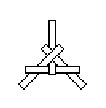
\includegraphics{provlavk}\\

\noindent
Dvě stejné číše jsou naplněny až po čárku, označující 
míru - jedna vínem a druhá limonádou. Vezmeme-li z~číše 
naplněné limonádou plnou lžíci a dáme-li její obsah do číše s~vínem, 
promícháme ji a pak opět plnou lžíci této směsi dáme do limonády, 
bude v~číši s~vínem větší procento limonády než 
procento vína v~číši s limonádou?\\[1 mm]
{\sl V~číši s~vínem bude stejné množství limonády,
jako množství vína v~číši s~limonádou.}\\

\noindent
Kde je na světě místo čtyř světových stran jen jedna 
světová strana?\\[1 mm]
{\sl Na severním pólu je jen jih, neboť kam se podíváme, je to 
vždy jižním směrem. Podobně je na jižním pólu jenom sever.}\\

\noindent
Jak je možno udělat ze dvou tyčí deset, aniž by se zlomily.\\[1 mm]
{\sl Dáme-li dvě tyče přes sebe, vznikne X, římsky 10.}\\

\noindent
Je v~moři více písku nebo ryb?\\[1 mm]
{\sl V~moři je více ryb, písek je pod mořem.}\\

\noindent
,,Závodník snědl tři vejce na lačný žaludek a pak se rozběhl.`` 
Ve větě je chyba. Kde?\\[1 mm]
{\sl Závodník mohl sníst na lačný žaludek jen jedno vejce, při
dalších už nebyl žaludek lačný.}\\

\noindent
V~knihovně jsou zařazeny tři díly jistého šíleného 
románu. Mají 296, 274 a 548 stran. Každý list je silný 0,12 mm 
a jedna deska s~předsádkou 2 mm. Jaká je vzdálenost od 
prvé strany prvého dílu k~poslední straně druhého dílu?\\[1 mm]
{\sl Vzdálenost je 4 mm. Horní deska s~předsádkou prvního 
dílu a spodní deska s~předsádkou druhého dílu.}\\

\noindent
Majitel ranče odkázal majetek svým třem synům, přičemž 
stanovil, že se o 17 koní mají rozdělit tak, že nejstarší syn 
obdrží polovinu, prostřední polovinu a nejmladší devítinu. Synové 
se málem umlátili, protože jim dělení nějak nevycházelo. Sousedi 
na ně zavolali šerifa, který přijel brzy na rychlém ryzáku a 
snadno dědictví rozdělil. Jak to udělal?\\[1 mm]
{\sl Šerif přidal k 17 koním svého ryzáka, takže jich bylo 18. 
Z~nich dal polovinu (9) nejstaršímu, třetinu (6) prostřednímu,
devítinu (2) nejmladšímu synovi a svého koně si vzal zase zpět.}\\

\noindent
V~kolik hodin rozdělují ručičky hodinek ciferník 
na dva půlkruhy, v~nichž je v~každém stejný součet 
hodin (tj. součet čísel od 1 do 12)?\\[1 mm]
{\sl Přibližně v 9:17 a 3:49. Součty činí vždy 39.}\\

\noindent
Kupující platil za klobouk, který stál 50,- stokorunou. 
Protože obchodník neměl nazpět, šel bankovku rozměnit nazpět 
do blízké drogerie a pak návštěvníkovi vrátil 50,- Druhého dne 
se drogista přihlásil, že stokoruna je falešná a obchodník mu 
musel dát jinou. Jakou celkovou škodu obchodník utrpěl?\\[1 mm]
{\sl Přišel celkem o 100,- které musel dát drogistovi místo falešné 
stokoruny. Za klobouk mu zůstalo 50,- od drogisty.}\\

\noindent
Bystrý je-li luštitel náš mladý, neztroskotá v~tomto 
taji. 85 let dohromady dědeček s~vnukem prý mají. O 65 let přitom
děda více má než vnouče jeho. Jak stár je vnuk řešení se hledá,
není to nic nesnadného.\\[1 mm]
{\sl Vnukovi je 10 a dědovi 75.}\\

\noindent
Dá-li Frantík Pepíkovi dvě kuličky, bude mít Pepík dvakrát 
tolik kuliček co Frantík. Dá-li Pepík Frantíkovi dvě kuličky, 
budou mít oba stejný počet. Kolik kuliček má Frantík a kolik 
Pepík?\\[1 mm]
{\sl Frantík má 10 kuliček a Pepík 14.}\\

\noindent
Napište jedním slovem suchá tráva.\\[1 mm]
{\sl Seno.}\\

\noindent
Co je mezi mořem a zemí?\\[1 mm]
{\sl Písmeno ,,a''.}\\

\noindent
Čtyřicet bez deseti je padesát. Jak je to možné?\\[1 mm]
{\sl V~římských číslicích: XL - X = L}\\

\noindent
Dobře se zamyslete a odpovězte. Je dříve dům postaven 
nebo zbourán?\\[1 mm]
{\sl Dům je dříve postaven, neboť bourat jej můžeme až po postavení.}\\

\noindent
,,Dcera se už bude vdávat, ačkoliv jsme slavili pětkrát 
její narozeniny a žádné jsme nevynechali,'' prohlásil tajuplně 
otec. Jak je to možné?\\[1 mm]
{\sl Dcera se narodila 29. února, má tedy narozeniny co 4 roky.}\\

\noindent
Je možné, aby polovina z 12 bylo 7?\\[1 mm]
{\sl V~římských číslicích dostaneme podélným rozpůlením 
čísla XII číslo VII.}\\

\noindent
Kterou rostlinu pozná snadno i slepý?\\[1 mm]
{\sl Kopřivu.}\\

\noindent
Čeho je v~kalamáři nejvíce?\\[1 mm]
{\sl Písmene ,,a''.}\\

\noindent
Dva otcové a dva synové byli na návštěvě. Při svačině 
před ně hostitelka předložila tři čaje a vybídla je, aby pili. 
Všichni najednou se napili. Jak je to možné?\\[1 mm]
{\sl Jsou to dědeček, syn a vnuk (tedy pouze tři osoby).}\\

\noindent
Dvanáct mincí leží jako na číselníku hodin. Vašim úkolem je 
přemístit mince tak, aby od 1 do 6 ležely dvě mince na sobě. 
Mince se přemisťují skokem přes dvě mince ležící vedle.\\[1 mm]
{\sl 12$\rightarrow$3, 7$\rightarrow$4, 10$\rightarrow$6, 8$\rightarrow$1, 
9$\rightarrow$5, 11$\rightarrow$2}\\

\noindent
V kruhu leží 18 zápalek a jako 19 je krabička. Vašim úkolem 
je odkudkoli odpočítat 6 sirek, šestou vzít a počítat dál, až 
zůstane pouze krabička. S krabičkou se pracuje stejně jako se 
sirkami.\\[1 mm]
{\sl Jako první se vezme 11. Zápalka od krabičky.}\\

\noindent
Vyjmenujte 5 po sobě jsoucích dnů, jejichž jméno neobsahuje 
U ani K.\\[1 mm]
{\sl Předevčírem, včera, dnes, zítra, pozítří}\\

\noindent
Jak udělat ze čtyř karetních pětek čtyři čtverky. Některou 
kartou něco zakrýt.\\[1 mm]
{\sl Karty se položí do kříže (kruhu), každá karta zakrývá své 
sousedce jeden znak.}\\

\noindent
Jak položit na stůl tři sirky tak, aby se hlavičkami 
nedotýkaly stolu.\\[1 mm]
{\sl Utvoříme ze sirek trojúhelník, přičemž každá sirka bude za 
hlavičkou opřená o sirku vedlejší.}\\

\noindent
Mají v USA 1. máj?\\[1 mm]
{\sl Ano, vždy po 30. dubnu.}\\

\noindent
Kolik dnů narození zažije průměrně člověk?\\[1 mm]
{\sl Pouze jeden, v porodnici.}\\

\noindent
Některé měsíce mají 31 dnů, kolik jich má 28 dnů?\\[1 mm]
{\sl Všechny, tedy 12.}\\

\noindent
Je těžší kilo železa, nebo kilo peří?\\[1 mm]
{\sl Stejně, pokud vám nespadnou na nohu.}\\

\noindent
Je u nás legální oženit se znova se svou ovdovělou
manželkou?\\[1 mm]
{\sl Ne, protože muž, jehož žena je vdova, je mrtev.}\\

\noindent
Vydělte 30 číslem 1/2 a přičtěte 10. Kolik vám vyšlo?\\[1 mm]
{\sl 70, protože 30 děleno 1/2 je 60.}\\

\noindent
Když na misce leží 3 jablka a dvě odeberete, kolik jablek máte?\\[1 mm]
{\sl Dvě. Ty, co jste odebrali.}\\

\noindent
Doktor vám dal tři pilulky a řekl, že máte brát každou půlhodinu
jednu. Kolik minut uteče od první pilulky než si vezmete poslední?\\[1 mm]
{\sl 60. Začnete první pilulkou, o 30 minut později vezmete druhou
a po 30ti minutách poslední.}\\

\noindent
Farmář měl 17 ovcí a kromě devíti mu všechny pošly. Kolik mu
jich zůstalo?\\[1 mm]
{\sl 9, ostatní přece uhynuly.}\\

\noindent
Kolik zvířat každého pohlaví a druhu vzal Mojžíš na svou Archu?\\[1 mm]
{\sl Žádné, to přece nebyl Mojžíš, ale Noe.}\\

\noindent
Kolik dvoukorun je v tuctu?\\[1 mm]
{\sl 12 dvoukorun v tuctu dvoukorun.}\\

\noindent
Na jezírku rostou lekníny. Každé ráno se na hladině objeví $2\times$
tolik leknínů, než kolik tam bylo minulý den. Jezírko úplně zaroste
za 4 dny. Za jak dlouho bude porostlé jen z $1/4$?\\[1 mm]
{\sl Za 2 dny.}\\

\noindent
Napište pomocí šesti číslic 5 a základních aritmetických operátorů
(+ - * /) číslo 1000?\\[1 mm]
{\sl $(5+5)(5+5)(5+5)=1000$.}\\

\noindent
Doplňte číslice 0--9 místo písmenek. Každé písmeno reprezentuje 
jinou číslici: TO + TO + LÉTO + ALE = LETÍ.\\[1 mm]
{\sl 32 + 32 + 4532 + 041 = 4637}\\

\noindent
Doplňte číslice 0--9 místo písmenek. Každé písmeno reprezentuje 
jinou číslici: HLE + HAD + LEZE + NA = ZEMI.\\[1 mm]
{\sl 473 + 406 + 7383 + 90 = 8352}\\

\noindent
Doplňte číslice 0--9 místo písmenek. Každé písmeno reprezentuje 
jinou číslici: DÁME + SI + DO = NOSU.\\[1 mm]
{\sl 6941 + 52 + 60 = 7053}\\

\noindent
Dvojice robotů stojí před naprosto stejnými dveřmi. Jeden ze strojů na tebe
obrátí pohled a řekne: ,,Pravé dveře jsou ty, které potřebuješ.''\\
,,Neposlouchej ho,'' radí ti druhý, ,,lže.''\\
,,Ale jenom někdy,'' reaguje první.\\
Kterými dveřmi půjdeš? Ze [\ref{gabook1}].\\[1 mm]
{\sl Máš jít pravými.}\\

\noindent
Mám tři zlaté truhlice. V každé z nich jsou tři stříbrné truhlice. V každé
stříbrné jsou dvě olověné truhlice. V každé olověné truhlici jsou tři dřevěné
truhlice, ve kterých už žádné truhlice nejsou. Do každé truhlice jsem vložil
jeden zlaťák a ještě tolik zlaťáků, kolik je v ní celkem všech truhlic. Kolik
mám zlaťáků ve všech truhlicích dohromady? Ze [\ref{gabook2}].\\[1 mm]
{\sl $3((1+3(1+2(1+3)))+3((1+2(1+3))+2((1+3)+3))) = 291$}\\

\noindent
Všichni duchové jsou strašidla a někteří duchové jsou obludy. Některé obludy
jsou lidožrouti, takže všichni lidožrouti jsou strašidla. Je to pravda,
nebo ne? Ze [\ref{gabook2}].\\[1 mm]
{\sl Nelze rozhodnout.}\\

\noindent
Mám dvě dcery. Až bude ta mladší tak stará, jako byla starší, když se mladší
narodila, bude zároveň dvakrát starší než je teď. Jaký je jejich věkový
rozdíl, když jim dohromady je 48 let? Ze [\ref{gabook2}].\\[1 mm]
{\sl Rozdíl činí 24 let.}\\

\noindent
Před půl hodinou bylo tři čtvrtě na osm. Kolik bude za hodinu?\\[1 mm]
{\sl Čtvrt na deset.}\\

\noindent
Ve škole je jedna vyučovací jednotka dlouhá 45 minut. Žáci mají 6 vyučovacích
jednotek denně. Kolik hodin se každý den učí?\\[1 mm]
{\sl Čtyři a půl hodiny.}\\

\noindent
Tramvaj přijíždí na zastávku každých 12 minut. První přijela v 9 hodin a 1
minutu. V kolik hodin přijede třetí tramvaj?\\[1 mm]
{\sl V 9 hodin, 25 minut.}\\

\noindent
Nádraží je od mého domu vzdáleno 6 kilometrů. Na kole jezdím rychlostí
12 km/h. Stihnu vlak, jestliže vyjedu 25 minut před jeho odjezdem?\\[1 mm]
{\sl Nestihnu, cesta na nádraží mi trvá 30 minut.}\\

\noindent
Vlak, který měl 20 minut zpoždění, přijel v 8 hodin a 12 minut. V kolik
hodin měl podle jízdního řádu vlak přijet?\\[1 mm]
{\sl V 7 hodin, 52 minut.}\\

\noindent
Za 6 minut bude tři čtvrtě na pět. Kolik bylo před 9 minutami?\\[1 mm]
{\sl Byly 4 hodiny, 30 minut.}\\

\noindent
Jsi v místnosti s jedinými dveřmi. Stojí zde tři sochy: medvěd, vlk
a ještěr. Klíč od dveří je v tlamě jedné ze soch. Musíš tam sáhnout a
klíč vytáhnout. Pokud sáhneš do tlamy, ve které klíč není, socha ti
ukousne ruku.\\
Pod sochami je 6 celkem nápisů, na každém podstavci dva. Na jednom
podstavci jsou oba nápisy nepravdivé, na dalším jsou oba pravdivé a na
zbývajícím je jeden nápis pravdivý a jeden nepravdivý.\\
U vlka je napsáno: ,,Já klíč nemám,'' a ,,Klíč je v tlamě medvěda.'' U
medvěda stojí: ,,Vlk nemá klíč,'' a ,,Klíč najdeš u ještěra.'' Nápisy pod
ještěrem hlásají: ,,Já klíč nemám,'' a ,,Klíč má vlk.''\\
Do které tlamy sáhneš pro klíč?\\[1 mm]
{\sl Klíč je v tlamě ještěra.}\\

\noindent
Na břehu řeky stojí farmář s ovcí, vlkem a hlávkou zelí. U břehu kotví jedna
malá loďka. Loďka je tak malá, že se do ní s farmářem vleze už buď jen koza,
jen vlk, nebo jen zelí.\\
Farmář chce dopravit všechen svůj majetek na druhou stranu. Protože ale vlci
žerou kozy a kozy mají rády zelí, nesmí zůstat bez farmáře na stejném břehu
vlk s kozou, ani koza se zelím.\\
V jakém pořadí má farmář svůj majetek převézt?\\[1 mm]
{\sl Koza tam -- vlk tam -- koza zpět -- zelí tam -- koza tam.}\\

\noindent
Na břehu řeky stojí 3 misionáři a 3 kanibalové. U břehu kotví dvojmístná
loďka. Všichni se chtějí dostat ve zdraví na druhou stranu. Zůstane-li na
jednom břehu více kabibalů než misionářů, kanbalové misionáře seřerou.\\
V jakém pořadí mají jezdit loďkou?\\[1 mm]
{\sl Dva kanibalové tam -- jeden kanibal zpět -- dva misionáři tam -- 
kabibal s misionářem zpět -- dva kanibalové tam -- jeden kabibal zpět --
dva kanibalové tam.}\\

\noindent
Na břehu řeky stojí pětičlenná rodina (syn, dcera, matka, otec a děda).
Přes řeku vede úzká kláda, přes kterou mohou jít současně nejvýše dvě osoby.
Každá osoba přejde přes kládu za jinou dobu. Synovi to trvá 1 vteřinu, dceři
2, matka přejde kládu za 6 vteřin, otec za 8 a děda za 12. Jdou-li dvě osoby
spolu, jdou rychlostí toho pomalejšího.\\
Protože je noc, musí mít ti, co jdou přes kládu, s sebou petrolejku. V lucerně
je ale palivo jen na 30 vteřin.\\
V jakém pořadí musí členové rodiny chodit přes kládu, aby se všichni stihli
dostat na druhou stranu, než lucerna zhasne?\\[1 mm]
{\sl Syn(1) a dcera(3) tam -- dcera(3) zpět -- otec(8) a děda(12) tam -- 
syn(1) zpět -- syn(1) a matka(6) tam -- syn(1) zpět -- syn(1) a dcera(3)
tam.}\\

\noindent
Aby získal ruku šachové princezny, musí princ na šachovém koni splnit nelehký
úkol. Zvolí si libovolné z políček na obrázku. Z něj pak musí skákat z
políčka na políčko tak, aby navštívil všechna ostatní políčka právě jednou
a posledním skokem se vrátit zpět na výchozí pole.\\
Žádné z políček (kromě prvního) nesmí navštívit dvakrát. V jakém pořadí
musí princ po políčkách skákat? Šachový kůň skáče vždy o dvě políčka dopředu
a jedno políčko doprava nebo doleva.\\[1 mm]
\begin{picture}(110,50)(0,0)
 \put(0,39){\framebox(10,10){}} \put(13,39){\framebox(10,10){}} \put(26,39){\framebox(10,10){}} \put(39,39){\framebox(10,10){}}
 \put(0,26){\framebox(10,10){}} \put(13,26){\framebox(10,10){}} \put(26,26){\framebox(10,10){}} \put(39,26){\framebox(10,10){}}
 \put(0,13){\framebox(10,10){}} \put(13,13){\framebox(10,10){}} \put(26,13){\framebox(10,10){}} \put(39,13){\framebox(10,10){}}
 \put(13,0){\framebox(10,10){}} \put(26,0){\framebox(10,10){}}
 \put(60,39){\framebox(10,10){10}} \put(73,39){\framebox(10,10){13}} \put(86,39){\framebox(10,10){6}} \put(99,39){\framebox(10,10){3}}
 \put(60,26){\framebox(10,10){5}} \put(73,26){\framebox(10,10){2}} \put(86,26){\framebox(10,10){9}} \put(99,26){\framebox(10,10){12}}
 \put(60,13){\framebox(10,10){14}} \put(73,13){\framebox(10,10){11}} \put(86,13){\framebox(10,10){4}} \put(99,13){\framebox(10,10){7}}
 \put(73,0){\framebox(10,10){8}} \put(86,0){\framebox(10,10){1}}
\end{picture}\\

\end{multicols}
\clearpage

% End of file


 % Written by Petr Gotthard
% Codepage ISO-8859-2

\section{Kvízové otázky}
\begin{multicols}{4}

\noindent
Tvarovat je\\
a) vyrábět tvaroh\\
b) tvářit se jako tvárnice\\
\textbf{c) dávat tvar nějakému předmětu}\\

\noindent
Kompost je\\
\textbf{a) hnojivo ze zbytků}\\
b) řecky ,,kompot''\\
c) kombinovaný poštovní balík\\

\noindent
Biologicky rozložitelný je\\
a) rozložená učebnice biologie\\
\textbf{b) produkt, který se lehce rozkládá v~přírodě}\\
c) rozkládací sedadlo v~kině\\

\noindent
Čistící stanice je\\
\textbf{a) místo, kde se čistí voda}\\
b) myčka aut v~servisu\\
c) stanice metra, kde dýcháme čistý vzduch\\

\noindent
Gravitace je\\
a) čistý vzduch\\
\textbf{b) zemská přitažlivost}\\
c) latinsky ,,rytina''\\

\noindent
Recyklování je\\
a) výměna pneumatik u bicyklu\\
b) oprava dráhy pro cyklisty\\
\textbf{c) přeměna použitého materiálu na novou základní surovinu}\\

\noindent
Nezfalšovatelné označuje\\
\textbf{a) něco, co nemůžeme napodobit}\\
b) věc, kterou lze těžko provést\\
c) někoho, koho nelze nikdy podplatit\\

\noindent
Svazek je\\
\textbf{a) soubor svázaných předmětů}\\
b) zkratka svazu ekonomů\\
c) svačina z~eidamu a kopru\\

\noindent
Papyrus je\\
\textbf{a) latinské slovo označující papír}\\
b) ruský dědeček\\
c) papírový pytel plný švábů rusů\\

\noindent
Braillovo písmo je\\
\textbf{a) písmo určené nevidomým}\\
b) rukopis irského mnicha\\
c) písmo, kterým je vytištěna nejstarší kniha světa\\

\noindent
Typy jsou\\
\textbf{a) písmena nebo znaky připravené k~tisku}\\
b) stany prérijních Indiánů\\
c) nepříjemní lidé\\

\noindent
Ve vesmíru máme\\
\textbf{a) rudý obličej}\\
b) vzduch\\
c) vodu\\

\noindent
Aerodynamika je\\
a) rychlý sport\\
\textbf{b) věda o odporu vzduchu}\\
c) prehistorický motýl\\

\noindent
Piktogram je\\
a) váha menší než jeden gram\\
b) latinsky ,,zloděj obrazů``\\
\textbf{c) kresba skrývající nějaký význam}\\

\noindent
Čočky jsou\\
\textbf{a) sklíčka nahrazující brýle}\\
b) malé hnědé luštěniny\\
c) čokoládové vločky\\

\noindent
Náprava je\\
a) nádrž právě naplněná\\
\textbf{b) příčná součástka, jež drží kola}\\
c) dopravní značka ukazující doprava\\

\noindent
Vrtačka je\\
a) dívka, která všechno pokazí (zvrtá)\\
\textbf{b) nástroj sloužící k~vrtání}\\
c) středověká dětská hra\\

\noindent
Vodní hodiny jsou\\
\textbf{a) příbuzné hodin přesýpacích}\\
b) čas strávený ve vodě\\
c) stroj na měření času používaný vodníky\\

\noindent
Mikroprocesor je\\
\textbf{a) elektronický mozek}\\
b) zpěvák, který nikdy nezpívá bez mikrofonu\\
c) mikrob, který procestoval svět\\

\noindent
Integrovaný obvod je\\
\textbf{a) elektronický mozek}\\
b) závodní dráha formule 1\\
c) obvod hlavy génia\\

\noindent
Co jsou to patáky ?\\
\textbf{a) Moravsky ,,lékařské prášky``}\\
b) Vysoké jezdecké boty\\
c) Valašské krojové klobouky\\

\noindent
Jak často nastává příliv?\\
a) 1 krát denně\\
\textbf{b) 2 krát denně}\\
c) 2 krát za měsíc\\

\noindent
Čemu se říká opičí hlavolam?\\
a) Tropický pavouk\\
b) Rozcvičovací cvik mimů\\
\textbf{c) Strom blahočet chilský}\\
(má tak rostlé větve, že na něj ani opice nemohou vylézt)\\

\noindent
Jak vytvářejí včely vosk?\\
\textbf{a) Zadečkem}\\
b) Vyvrhují jej ústním otvorem\\
c) Míšením slin s~pryskyřicí stromů\\

\noindent
Šachy pocházejí z \\
a) Arábie\\
\textbf{b) Indie}\\
c) Persie\\

\noindent
První poštovní známky byly roku 1840 vydány v \\
a) Rakousku\\
b) Francii\\
\textbf{c) Anglii}\\

\noindent
Bůh Radegast symbolizoval podle starých Slovanů \\
\textbf{a) Slunce, oheň}\\
b) Bojovníka\\
c) Pokušitele\\

\noindent
Pověst vypráví, že jméno hotelu Zlatá Husa na Václavském náměstí 
vzniklo podle \\
a) Zlatého pokladu ve tvaru husy nalezeného ve sklepení\\
\textbf{b) Přihlouplé dcery tamního hostinského}\\
c) Gurmánské speciality\\

\noindent
Jezuitský řád byl založen \\
a) Sv. Augustinem\\
b) Sv. Dominikem\\
\textbf{c) Sv. Ignácem z~Loyoly}\\

\noindent
Kolik mostů bylo v~Praze na počátku 19. století\\
\textbf{a) 1}\\
b) 2\\
c) 3\\

\noindent
Šampaňské se poprvé podávalo ve století \\
a) 10.\\
\textbf{b) 17.}\\
c) 18.\\

\noindent
Muslimský svátek Ramadán trvá\\
a) Týden\\
b) 14 dnů\\
\textbf{c) Měsíc}\\

\noindent
Benátský cestovatel Marco Polo podnikl se svým otcem a~strýcem 
cestu do Číny ve století\\
a) 12.\\
\textbf{b) 13.}\\
c) 14.\\

\noindent
První film Charlieho Chaplina nese název\\
\textbf{a) Chaplin si vydělá na živobytí}\\
b) Kid\\
c) Chaplin tulákem\\

\noindent
Hora Říp je z \\
a) Žuly\\
b) Břidlice\\
\textbf{c) Čediče}\\

\noindent
Románská rotunda na vrcholu hory Říp se jmenuje rotunda\\
\textbf{a) Sv. Jiří}\\
b) Sv. Vojtěcha\\
c) Sv. Václava\\

\noindent
Hvězdu Aldebaran by jste hledali v~souhvězdí\\
\textbf{a) Býka}\\
b) Berana\\
c) Orla\\
(je nejjasnější hvězdou)\\

\noindent
Který z~uvedených kopců je nejvyšší?\\
a) Milešovka (České středohoří)\\
\textbf{b) Praha (Brdy)}\\
c) Javořice (Českomoravská vysočina)\\
(Praha 863, Milešovka 837, Javořice 837)\\

\noindent
Kokoška pastuší tobolka kvete\\
a) Modře\\
b) Žlutě\\
\textbf{c) Bíle}\\

\noindent
David Livingstone, slavný cestovatel se proslavil svými cestami 
po\\
\textbf{a) Africe}\\
b) Austrálii\\
c) Polárních končinách\\

\noindent
Známé soustroví Galapagos leží svou větší částí\\
\textbf{a) Jižně od rovníku}\\
b) Severně od rovníku\\

\noindent
Přívlastek NEVALNÝ vznikl v~souvislosti se\\
\textbf{a) Zmačkanou látkou, která se špatně válela}\\
b) Latinským ,,valere'', mít hodnotu\\
c) Záporem slovesa volit\\

\noindent
Slovo MANŽEL vzniklo ze\\
a) Staroněmeckého ,,Mannesseele'' (mužská duše)\\
b) Francouzského ,,manchelle'', což byl mužský svatební kabát 
s~dlouhými rukávy\\
\textbf{c) Staročeského ,,malženstvo'' (mladoženství)}\\
(označovalo jak manželský stav tak i~celý pár)\\

\noindent
Krápavka je \\
a) Krápníkový útvar vzniklý prokapáváním vody uvnitř staveb, 
např. tunelů\\
b) Drobná žába žijící ve středomoří\\
\textbf{c) Skleněná trubička používaná v~laboratořích pro 
odkapávání drobných kapek (pipeta)}\\

\noindent
Slovo POTENTÁT (tj. panovník nebo významný hodnostář) má následující 
původ\\
a) Každý se z~něj potentuje\\
b) Z~latinského ,,potens'' (mocný)\\
c) Z~německého ,,Bodenteider'' (ochránce země)\\

\noindent
Slovo KLUK původně označovalo\\
a) Luk\\
\textbf{b) Šíp}\\
c) Sekeru používanou pro klučení lesů\\
(neopeřený šíp, který daleko nedoletí, později přeneseno na nezralou 
mládež)\\

\noindent
Baldachýn se jmenuje podle\\
\textbf{a) Bagdádu, odkud byla dovážena na něj látka}\\
b) Čínských bálů, francouzsky ,,Bal de Chine''\\

\noindent
Cereálie jsou\\
a) Sušené celerové kostičky\\
\textbf{b) Obilniny}\\
c) Druh mořských sasanek\\

\noindent
Glycidy jsou pro organismus zdrojem\\
\textbf{a) Energie}\\
b) Vody\\
c) Glycerinu\\

\noindent
Z celkového denního energetického příjmu by měla snídaně tvořit\\
\textbf{a) 20 \%}\\
b) 30 \%\\
c) 50 \%\\

\end{multicols}
\clearpage

% End of file

 \section{Kouzlení a čarování}

\subsection{Pomůcky}

Kouzelnická hůlka je dřevěná, kulatá 30 cm dlouhá tyčka. Celá 
černě lakovaná, jen 6 cm obou konců je bílých.

\subsection{Kouzla humorná}

\nadpis{Fakir}{cokouzla}
Palec překryji šátkem a začnu do něj bodat jehlice a 
špendlíky. Pak je zase vytahám, palec odkryji a vše je v~naprostém 
pořádku.

Palec z~rukavice něčím vycpaný je jemně nastehován 
na šátek. Když palec přikrývám, pod kapesníkem palec ohnu a do 
prstů sevřu spodní konec látkové napodobeniny. Napodobenina musí 
být vždy schovaná v~šátku, divák ji nesmí vidět.


\nadpis{Jasnovidec}{cokouzla}
Řekneme, že uhádneme, co si kdo myslí. Do řady postavíme 
tři dobrovolníky a připravíme tři mince. Prvnímu dobrovolníkovi 
řekneme: ,,Dám vám teď minci, pevně ji sevřete v dlani.`` A dáme 
mu minci. U druhého postup zopakujte. Třetímu však nic neříkejte, 
jen viditelně držte poslední minci. Divák otevře dlaň a nastaví 
ruku. Ukažte na něj hůlkou a řekněte: ,,Tento divák si myslí, 
že také dostane minci.``


\nadpis{Jasnovidka}{cokouzla}
Kouzelnice požádá několik diváků, aby napsali na papír 
několik slov. Oni pak odevzdají asistentce, která je složí, vloží 
do klobouku a odevzdá jasnovidce. Ta papíry vytahuje, čte slova 
a říká, zda je psala žena či muž.

Trik spočívá ve skládání papíru. Papír lze nejprve přehnout 
ve svislé nebo ve vodorovné ose. Podle toho jasnovidka pozná 
pisatele.


\nadpis{Jasnovidec}{cokouzla}
Diváci se domluví na nějakém slově a já je uhádnu.

Kouzelník ukazuje náhodně na diváky a ti mají za úkol říkat 
různá slova. Kouzelník je však domluven s~pomocníkem, 
který říká slova, jejichž první písmeno je vždy obsaženo v hledaném 
slově. Je-li slovo celé, řekne pomocník předem dohodnuté slovo.

Př. Slovo=řemen, pomocník hlásí Řád, Eskymák, Mlha, Ešus, Noha.


\nadpis{Kuličky}{cokouzla}
Z papíru 3$\times$3 cm utvořte tři kuličky a položte si je do 
žlábku mezi dvěma prsty. Pak foukněte a všechny kuličky spadnou. 
Teď se zeptejte, která kulička má zůstat na svém místě při dalším 
fouknutí. Zamávejte nad ní hůlkou,přidržte ji a foukněte. Diváci
pochopí žert, vy však buďte ochoten pokus opakovat s jinou kuličkou.


\nadpis{Kolik je 7$\times$7}{cokouzla}
Utvoříme si kartičku 7$\times$7 a rozstříháme ji podle prvního
obrázku. 7$\times$7 je teď 49. Poskládáme-li však rozstříhanou
kartičku podle druhého obrázku, přesně jeden čtvereček bude
chybět. 7$\times$7 je tedy 48.\\
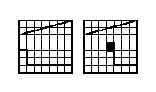
\includegraphics{kolik7x7}


\nadpis{Pravopisný chyták}{cokouzla}
Ať se přihlásí ten, kdo si myslí, že zná dobře český pravopis. 
Nadiktujeme mu pak k napsání tuto větu: Kočí zvedl bič a zvolal: 
Hyje, koníčky...  (na konci mlaskneme jazykem jako na koně). 
Mlasknutí se ještě nikomu nepodařilo napsat a ani nepodaří.


\nadpis{Silné nervy}{cokouzla}
,,Kdo z vás vydrží pod stolem do kterého 3x za sebou prudce 
udeřím dlaní?'' Určitě se nikdo najde a vleze si pod stůl. Ty 
pak udeř do stolu ale jen dvakrát. ,,Tu třetí ránu dám až za 
týden, jsem sám zvědav, jestli odvážlivec tam tak dlouho vydrží 
!''


\subsection{Kouzla vážná}

\nadpis{Prostupnost hmoty}{cokouzla}
Mám šňůrku a na jejích koncích korálky. Vezmu sklenici 
s~velkým uchem dnem vzhůru. Šňůrku položím na levou ruku 
tak, že její střed spočívá mezi nataženým palcem a ukazováčkem 
a tvoří mezi nimi proužek. Na šňůrku položím ucho sklenice, zatlačím, 
korálky se mírně zvednou. Pak sklenici pustím a ona zůstane viset.

Když tlačíme ucho proti šňůrce a tím vytahujeme korálky, 
vyprostíme palec, takže stuha visí je na ukazováku. Poté vsuneme 
ucho mezi palec a šňůrku a vsuneme palec uchem zase pod šňůrku. 
Tlačíme dál, až se nám dostanou korálky do dlaně. Teď sklenici 
pustíme. Jeden korálek se provleče uchem, šňůrka se napne a sklenice 
zůstane viset.


\nadpis{Čtenář myšlenek}{cokouzla}
Oznámíte všem, že jste čtenář myšlenek, o čemž je hned 
přesvědčíte. Vyzvete je, aby každý napsal na list papíru nějaké 
přísloví nebo libovolnou větu o pěti slovech (ne více), dal ji 
do obálky a zalepil. Potom obálky seberte, jednu po druhé přikládejte 
na čelo, soustředíte se, tváříte se důmyslně a k úžasu přítomných 
čtete věty v nich obsažené.

Je třeba abyste byli předem smluveni s některým z hráčů. 
Když přiložíte první obálku na čelo, nevíte sice co je v ní napsáno, 
ale znáte větu, kterou jste si předem smluvil se svým tichým 
společníkem a tuto větu řeknete jako první. Když pak obálku ,,pro 
kontrolu'' otvíráte, seznámíte se s obsahem věty, kterou 
napsal jiný účastník a přisoudíte ji další obálce. Po skončení 
celé atrakce se mohou účastníci přesvědčit, že všechny věty, 
které jste přečetl, jsou skutečně na lístcích napsány. Při otvírání 
obálek je nutno dát bedlivý pozor, abyste obálku se smluvenou 
větou otevřeli jako poslední. Je dobře, když obálky i lístky 
papíru jsou stejné, aby některý z diváků nepoznal trik. Pokud 
chceme ušetřit obálky, musí všichni hráči svůj papír složit stejným 
způsobem a to tak, aby nebyl vidět text.


\nadpis{Sirky ve vzduchu}{cokouzla}
Ukážu ruce, sáhnu do vzduchu a objevím sirku, hodím 
ji do klobouku a už vytahuji za zády další sirku, kterou opět 
házím do klobouku a to už... Pak z klobouku vysypu celou hrst 
sirek

Z průhledné lepicí pásky si zhotovím lepicí prstýnek a nasadím 
na prostředník. Jakmile ukážu ruce, nalepím na prstýnek ze strany 
nehtu sirku. Jsou-li prsty nataženy, sirka není vidět. Hmátnu 
tedy do vzduchu, skrčím prsty a objevím sirku. Objevenou sirku 
přidržím palcem. Ruku vstrčím do klobouku, kde prsty narovnám. 
Tím se sirka zase schová a já ji mohu zase někde najít. Nakonec 
sirku palcem odlepím, hodím tentokráte doopravdy do klobouku 
a z klobouku vysypu sirky, co jsem tam měl již nachystány.


\nadpis{Dámy utekly}{cokouzla}
Ukážeme několik karet a mezi nimi dvě dámy. Řekneme, 
že dámy nemají rády, když to a to. Pak karty složíme a převážeme 
gumičkou. Uděláme to a to. Poté gumičku odstraníme a vida, dámy 
jsou pryč. Pak je někde objevíme.

K tomuto kouzlu je nutné si připraviti preparovanou kartu. 
Z obou dam odstřihneme horní pětinu karty a slepíme je k sobě. 
Mezi ostatními kartami (ukazujeme sloupec karet) vypadají normálně. 
Když ale karty skládáme, přehneme preparované dámy a schováme 
je v dlani. Jakmile sáhneme do kapsy pro gumičku, necháme dámy 
v kapse. Před představením někde uschováme dvě normální dámy, 
které pak náhodou objevíme.


\nadpis{Kde je těžiště}{cokouzla}
Kouzelník vezme dlouhou krabičku a z malé části ji položí 
na sklenici, krabička však nespadne.

U jednoho konce krabičky je připevněno olůvko, které přesunuje 
těžiště, takže se sklenice nepřeváží.


\nadpis{Kdo postaví krabičku}{cokouzla}
Prázdná krabička od sirek je položena na kraji stolu 
tak, že ji kousek přečnívá desku stolu. Kouzelník ji zespodu 
jedním prstem postaví. Ukáže krabičku, že je zcela normální. 
Když krabičku zkouší postavit divák, vždy se mu převáží dozadu.

Krabička na stole leží vždy obrázkem nahoru. Je-li dno její 
zásuvky blíže k desce stolu, krabičku lze postavit, je-li však 
zásuvka zasunuta obráceně, krabička se vždy převáží.


\nadpis{Matematický omyl}{cokouzla}
Divák má sčítat po řadě čísla 1000 + 30 + 1000 + 30 + 
1000 + 30 + 1000 + 10. Téměř všichni odpoví, že výsledek je 5000, 
ačkoli je 4100.

Divák prostě podlehne pravidelnosti a svůj omyl si neuvědomí.


\nadpis{Mince je pryč}{cokouzla}
Položíme minci na táce, přikryjeme šátkem a obejdeme 
diváky. Každý vsune ruku pod šátek a řekne, zda tam mince skutečně 
je. Potom uděláme abrakadabra a zvedneme šátek. Mince zmizela. 
Obdobným postupem se mince na tácku opět objeví.

Ke kouzlu je zapotřebí pomocníka, jemuž jako poslednímu tácek 
ukazujeme. Ten minci v první fázi vezme, schová a řekne, že tam 
je. Ve druhé fázi minci na tácek položí a řekne (jako všichni 
ostatní), že tam mince není.


\nadpis{Najdu správnou kartu}{cokouzla}
Karty jsou seřazeny do 3 sloupců po 7 kartách. Divák 
si vybere kartu a ukáže na sloupec, ve kterém se nachází. Totéž 
pak udělá ještě 3x. Pak mu kouzelník slavnostně ukáže jeho kartu.

Karty je nutné sbírat po sloupcích tak, aby divákem označený 
sloupec byl vždy uprostřed. Po třetím posbírání je karta je jedenáctá 
ať se počítá z kterékoli strany.


\nadpis{Očarovaný řetěz}{cokouzla}
Dvojitý řetěz držím ve svislé poloze. Druhou rukou vezmu 
kroužek, pustím jej a on propadne a zastaví se dole jako poslední 
článek řetězu.

Asi ze třiceti kroužků sestavíme řetěz následovně. Do jednoho 
kroužku navlékneme dva další. Pak řetěz přetočíme o 90$^\circ$ 
doprava. Do zadního kroužku navlékneme další kroužek a oběma 
(zadním i předním) provlékneme druhý kroužek. Řetěz opět přetočíme 
o 90$^\circ$ doprava a pokračujeme v sestavování. Do zadního 
kroužku... Poslední kroužek je navléknut do obou kroužků předchozího 
článku.

Palec a ukazovák levé ruky pevně drží jednotlivý horní kroužek. 
Palec a ukazovák pravé ruky uchopí pravý kroužek pravého páru 
(je v něm navléknut pouze jeden kroužek druhého páru) Horní jednotlivý 
kroužek pustíme a ten zdánlivě prostoupí celým řetězem a umístí 
se jako poslední dole. Přitom řetěz přetočíme zase o 90$^\circ$ 
a horní kroužek uchopíme levou rukou. Palec a ukazovák pravé 
ruky uchopí pravý kroužek pravého...


\nadpis{Přimražená sklenice}{cokouzla}
Na sklenici úplně plnou vody přiložíme papír a zrcátko. 
Pak foukneme ,,studený vítr`` a posečkáme. Sklenice za určitou 
dobu přimrzne k zrcátku.

Papír je savý piják, voda převařená. Papír vysává vodu, tím 
vzniká podtlak a sklenice drží.


\nadpis{Sirka dělá stojku}{cokouzla}
Kouzelník má v ruce sirku, postaví ji hlavičkou na podložku, 
pronese kouzelné slovo a sirka stojí.

Potají si nasliníme nehet, ten pak v nestřeženém okamžiku 
třeme o hlavičku sirky, čímž ji navlhčíme. Takováto sirka vydrží 
stát na vhodné podložce (papír, látkový ubrus) velmi dlouho.


\nadpis{Sklenice propadne stolem}{cokouzla}
Kouzelník vezme sklenici, přikryje je ji šátkem. Pak 
nakreslí na stůl křížek a položí sklenici na něj. Sklenice však 
propadne stolem, spadne na zem a rozbije se.

Kartónové kolečko stejného průměru jako vrchol sklenice nastehujeme 
na šátek. Když bereme sklenici pod šátkem, chytneme sklenici 
i kartónek. Ve chvíli, kdy kreslíme křížek, pustíme sklenici 
do klína (díky šátku nepozorovaně). Kartónek stále držíme, takže 
to vypadá, jako by se nic nestalo. Pak už jen stačí, když pokládáme 
,,jako sklenici`` na stůl, pustit z klína sklenici na zem.


\nadpis{Voda mění barvu}{cokouzla}
Ve sklenici je červená voda. Sklenici přikryjeme šátkem, 
zakouzlíme. Když zvedneme šátek, je ve sklenici voda čirá. Přelijeme 
vodu z jedné sklenice do druhé a vida --- voda je zase červená.

Ve sklenici je vložka z červené hmoty vysoká přesně na výšku 
hladiny. Když snímáme šátek, vyjmeme zároveň i vložku, takže 
voda je bílá. Ve druhé sklenici je KMnO$_4$, ten vodu obarví opět 
na červeno.


\nadpis{Výroba zlata}{cokouzla}
Podivným činěním vytvoříme zlato.

Roztok octanu olovnatého v jedné baňce a jodidu draselného 
v baňce druhé zahříváme na teplotu varu. Slijeme obě tekutiny 
barvy čisté vody dohromady. Jakmile začne směs chladnout, objeví 
se na dně krystalky ,,zlata''.


\nadpis{Zmizelé mince}{cokouzla}
Na stole leží mince. Vezmeme plechový tácek, shrneme 
na něj zmiňované mince. Mince při dopadu na tácek zvoní, ale 
když jej ukážeme divákům, nic na něm není.

Asi 10 cm pod úrovní desky stolu je plech. Mince tedy zvoní, 
jako kdyby dopadaly na tácek, ve skutečnosti však dopadají na 
plech.


\nadpis{Modrý --- červený}{cokouzla}
Karetní hru rozevřu do vějíře a ukážu z~obou stran. 
Diváci vidí karetní hru s~modrým rubem. Pak karty shrnu 
do balíčku, modrou kartu odeberu, červenou přidám, karty zase 
rozevřu a už mají rub červený.

Karty preparujeme následujícím způsobem. Oddělíme ruby a 
úhlopříčně je rozstřihneme a pak zase slepíme. Lepíme však tak, 
že na jedné kartě je polovina červeného a polovina modrého rubu. 
Slepené karty zatížíme. Dvě karty takto nepreparujeme. Když karty 
rozevřeme, ukážeme vždy jednu polovinu rubu. Jen horní (jedna 
z~nepreparovaných) je vidět. Pak karty složíme a vodorovně 
odložíme. Poté sejmeme modrou nepreparovanou a nahradíme ji červenou, 
rovněž neupravenou kartou. Mezitím je nutné karty otočit. Když 
vějíř zase rozevřeme, vidí diváci tentokráte druhou polovinu 
rubu preparovaných karet.


\nadpis{Colombovo kouzlo}{cokouzla}
Vyzvěte diváka, aby si myslel číslo od 1 do 4 a pak vám 
je řekl. Na důkaz své jasnozřivosti vyzvěte diváka, aby se podíval 
na určité skryté místo, kde nalezne cedulku: ``Věděl jsem, že 
si myslíte číslo...''.


Na různých skrytých místech jsou umístěny cedulky pro všechna 
přípustná čísla. Podle čísla, které si myslel, vyšle diváka kouzelník 
na místo s~patřičnou cedulkou.


\nadpis{Jasnovidec}{cokouzla}
Vybraný divák si bude myslet číslo od 1 do 4 (lze i více). 
Kouzelník se chvíli soustředí a pak řekne: ,,Už vím, jaké 
číslo si myslíte. Řekněte mi je.'' Divák řekne své myšlené 
číslo. ,,A teď se podívejte pod talíř,'' řekne kouzelník. 
Divák pod talířem nalezne cedulku: ,,Věděl jsem, že si 
myslíte číslo...''

Pokud by divák řekl, že si myslel jiné číslo, poslal by ho 
kouzelník podívat se pod jiný předmět. Kouzelník má totiž připraveny 
pod různými předměty cedulky pro všechna možná čísla. Předmětů 
by mělo být mnohem více než čísel.


\nadpis{Kapsa plná karet}{cokouzla}
Divák vytáhne z~balíčku 3 karty a zapamatuje si 
je. Kouzelník si karty vloží do kapsy, potom dvě vytáhne a požádá 
diváka, aby řekl jednu z~karet, které si vytáhl. Kouzelník 
potom vytáhne z~kapsy třetí kartu --- a je to přesně ta, 
jakou určil divák.

Kouzelník si karty vloží do kapsy a přitom si zapamatuje 
jejich pořadí. Potom vytáhne z~kapsy dvě jiné karty, které 
už v~kapse byly. Jakmile řekne divák své přání, bez problémů 
vytáhne patřičnou kartu.


\nadpis{Létající mince}{cokouzla}
Před zraky diváků postav na prázdnou sklenici talířek. 
Přes všechno pak přehoď šátek. Nyní vezmi do levé ruky korunu 
a dej ji do druhé ruky a zároveň ji vyhoď do výšky. Vezmi kouzelnickou 
hůlku a začni vysvětlovat, že mince lítá ve vzduchu a že jí hůlkou 
stáhneš přes talířek do sklenice. Hůlkou se dotkneš a uvolněná 
mince spadne s cinknutím na dno sklenice.

Při pokládání talířku na sklenici přidrž nenápadně na dně 
talířku přidrž korunu a přimáčkni ji mezi talířek a sklenici. 
Do levé ruky vezmi jinou korunu, naoko ji dej do druhé ruky a 
naznač její vyhození do vzduchu. Mezitím ukliď z levé ruky korunu 
do kapsy. Hůlkou se potom dotkni talířku na okraji, tím ho na 
druhé straně nadzvedneš a mince spadne do sklenice.


\nadpis{Matematický trik}{cokouzla}
Kouzelník předloží kartičku s~čísly. Divák si vybere 
jedno číslo a zatrhne všechna čísla v řádku a sloupci, kde se 
zvolené číslo vyskytuje (10). Pak si vybere číslo ještě nezatržené 
a postup opakuje (4). Součet zbylých čísel je vždy 40.


\nadpis{Pravdomluvné zrcadlo}{cokouzla}
Vyhlídni si předem svou oběť, na kterou napiš křídou 
na zrcadlo nějaký vtip. Vše pak smaž hadrem, takže sklo se jeví 
jako čisté. Pak přede všemi vyzvi svou oběť aby se podívala do 
zrcadla a řekla co vidí. Samozřejmě, že uvidí jen sama sebe. 
Řekni, že zrcadlo je kouzelné, ale ten co se do něj dívá se musí 
napřed otočit 3x doprava, pak 3x doleva a nakonec na zrcadlo 
3x dýchnout. Pak mu zrcadlo něco poví.


\nadpis{Rentgenový zrak}{cokouzla}
Kouzelník se otočí, diváci položí na stůl minci a přikryjí 
ji neprůhledným hrnečkem. Kouzelník se zamyslí a pozná, jaká 
to je mince.

Pomocník a zasvěcenec, který minci přikrývá, nasměruje ouško 
hrnečku směrem podle toho, jaká mince pod hrnečkem je.


\nadpis{Šáteček a svíčka}{cokouzla}
Na stolek připrav větší nezapálenou svíčku a pootevřenou 
krabičku sirek. Svíčku zapálíme a krabičku sirek zavřeme. Hořící 
svíčku chytíme jednou rukou a druhou vytáhneme z~plamene 
šáteček.

Šáteček je nasoukán v~krabičce sirek. Svíčku zapálíme 
a krabičku sirek zavřeme, tím se dostane šátek nepozorovaně do 
dlaně. Není pak už nic snazšího, svíčku chytit rukou se šátečkem 
a druhou jakoby s plamene vytáhnout šáteček.


\nadpis{Zlomená sirka}{cokouzla}
Divák zlomí sirku, kouzelník ji zabalí do kapesníku, 
zakouzlí a divákova sirka je opět celá a neporušená.

Předem (mimo zraky diváků) zasuneme do lemu kapesníku jednu 
sirku. Pak požádáme někoho z diváků, aby nám donesl zdravou zápalku. 
Tu pak před všemi dáme doprostřed kapesníku a poznačíme fixem, 
aby nemohlo dojít k záměně. Pak kapesník překládáme ovšem tak 
šikovně, abychom dali divákovy přes kapesník do ruky sirku v 
lemu. Požádáme ho aby sirku zlomil. Po té kapesník rozbalíme 
a vyndáme a divákům ukážeme opět zdravou sirku.


\nadpis{Živá kouzelnická hůlka}{cokouzla}
Po krátké přednášce o důležitosti kouzelnické hůlky, 
vezmi láhev a hůlku do ní strč. Po magických slovech a pohybech 
volné ruky sama vylézá z~láhve.

Hůlku však předem za jeden konec přivážeme za nit. Ten pak 
strkáme do láhve. Druhý konec nitě zavážeme k opasku kalhot. 
Tím, že pohybujeme lahví, hůlka vystupuje či zajíždí do láhve. 

 % Written by Petr Gotthard
% Codepage ISO-8859-2

\section{Cvičení řeči}
\begin{multicols}{\value{columnsgames}}

\subsection{Jazykolamy}

\begin{itemize}
\itemsep -3pt

\item[-] Jen mi, kmotře Petře, toho vepře nepřepepřete. Jestli mi 
toho vepře, kmotře Petře, přepepříte, pak si toho vepře, kmotře 
Petře, snězte sám.

\item[-] Letělo tři tisíce tři sta třicet tři stříbrných křepelek přes 
tři tisíce tři sta třicet tři stříbrných střech.

\item[-] Naše lomenice je ze všech lomenic ta nejlomenicovatější.

\item[-] Drbu vrbu.

\item[-] Šel pštros s pštrosicí a s pštrosáčátky Pštrosí ulicí.

\item[-] Naleju-li oleje, nenaleju-li oleje.

\item[-] Já rád játra, ty rád játra.

\item[-] Řekl řek, kolik je v Řecku řek.

\end{itemize}

\subsection{Výslovnost}

\begin{description}
\itemsep 0pt

\item[S] V~sadě se pase husa s~housaty. Sova houká v~lese. 
V~létě spíme ve stanu. Sype, les, maso, sám, snaha, sníh,
písně, miska, píská, kokos, kompas, nos.

\item[Z] Koza leze do zelí. Zuzana veze vozík. Zdeněk má
zelený balón. Je zima. Zima, zebe, zase, zebra, zívá, zisk,
vozí, kazí, kozí, zbojník, zde, zdola, zob.

\item[C] Chlapec běžel na kopec. Koníci cválají do kopce. Alice cinká 
na poklice. Cena, cihla, necky, nic, domácí, ocel, ovoce, cítí, civí,
cibule, lovec, otec, kopec.

\item[S -- C] Malé selátko cucá. Cilka má dlouhé vlasy. Slunce svítí. 
Měsíc svítí v~noci. Cosi, cesta, silnice, slepice, myslivec, ocas,
sice, svícen, slunce, tisíc, soudce.

\item[Z -- S] Na podlaze jsou zase saze. Pes veze vozík. V~zimě 
jezdíme na saních. Zase, saze, zápis, zastaví, zasadí, zásuvka, zásoba, sazenice, svízel, smazal.

\item[C -- Z] Cilka nese záclony. Někdo zcizil peníze. Cizinec zabloudil 
na ulici. Co to cinká? Cizina, cizinec, cizí, zajíc, vzácnost, záclona,
zacpal, horolezec, jezdec, vzácný.

\item[Š] Náš Míša našel v~lese šišku. V~koši byly myšky. Hoši mají tašky.
Koš, máš, náš, voláš, šumák, koše, naše, škola, škytá, výška, jíška,
lepší, ještě.

\item[Č] Anička má ráda čokoládu. Mám míč a bič. Kolotoč se točí. Čpavek 
čpí. Oč, pláč, upeč, čočka, kočka, počká, čokoláda, čouhá, čumák, často,
čepel.

\item[Ž] Želva pomalu leze. Božena má nové lyže. Žížala leží u kaluže.
Žížala, žáci, žehlí, žena, žold, lože, lyže, vlažný, dlažba, dlužen, něžný,
žně.

\item[Č -- Š] Ušáček, Vašíček, košíček, šáteček, češe, čeština, školáček, 
kašička, mašlička.

\item[Ž -- Č] Nožička, žehlička, lžička, mužíček, nožíček, čížek, kůžička, 
žehlička, nožíček.

\item[C -- Č] Čepice, cvičky, cvičí, Aničce, kočce, cvičitel, cvočky, 
čepice, tetičce, kočce.

\item[S -- Š] Sušenka, suší, sešit, sluší, snáší, soška, štěstí, šije 
se, slušně, šťastný, šosy.

\item[Z -- Ž] Zamaže, zaváže, železo, žízeň, zboží, zběžný, žíznivý,
žaluzie, žezlo.

\item[Š -- C] Švec, náušnice, myšce, lišce, o myšce, maceška, ve výšce, 
šicí, pšenice.

\item[S -- Ž] Sváže, sjíždí, složí, spolužák, sněží, snížek, užaslý,
možnosti, žalost, smaží.

\item[Č -- S] Číslo, čistí, slečna, sáček, měsíček, louskáček, sčítá součet, 
svačí, skučí, skoč.

\item[L] Nad lesem letí letadlo. Bylo bláto. Nebyla celá bílá. Slimák 
se schoval. Lípa, loďka, plakal, láme, lano, laň, louka, dál, vál, sál,
ukládá, klopýtá, kluk.

\item[R] Petr pracuje v~továrně. Traktor má silný motor. U hradu 
byl ukrutný drak. Kotrmelec, strašný, vrznout, fraška, brada, brzo, brýle, hromada, hrbol.

\item[Ř] U řeky roste řepa. Stařeček řeže dříví. Zavři pusu, Petříku. Zahřmělo.
Dřímá, truhlář, třpytka, natřásl, příběh, příchod, přijal, přejel, křižovatka.

\item[P] Pavel pracuje v~továrně. Petr propíchl peřinu. Pepa stojí 
pod lípou. Popel, pálí, Petr, pampeliška, pomalu, pec, pivo, popleta,
papoušek, páv.

\item[B] Bába Bulíková šla do lesa na houby. Béďa peče bábovku. Kubu 
bolí zoubek. Bude, bledý, bída, bouda, hubený, houba, obutý, obilí, obálka, 
Kuba, kabát.

\item[D] Máme doma dudy. David jede domů. Teta mi dala domino. Tady je 
dům. Odpoledne, domov, sudy, dudlík, dávno, datum, dech, doutnák, 
doupě, den.

\item[T] Teta stojí u stolu. Kotě v~botě tiše kouká. Potom chytí 
klubko nití. Teče, tulipán, také, kabát, nitky, kvítky, látky, kabátky,
Tonda, boty, tahat.

\item[M] Máma má malé dítě. My máme maso v~míse. Máma mele pro 
mne mák. Moje, med, mísa, Míša, mouka, máma, mnoho, málo, mák, pomocník.

\item[N] Naše Nána nosí noviny. Punťa chňapl po pečeni. Jeník měl sáně.
Noc, nový, nůše, neděle, nehoda, panenka, venku, nenapomene, nechce.

\item[H] Honza Hynek nosí hodinky. Helena hledá houby. Hbitý Haf pobíhá.
Hůl, hádá, hladí, nohy, hádanka, honem, hodnota, houska, hmota, hlava.

\item[CH] Chlapci chodí na chůdách. Hluchý lachtan delfínem je lechtán.
Chová, chechtá, chochol, buchta, chuť, chasa, chapadlo, pech, suchá.

\item[K] Karel Kovář seká sekyrou. Alenka kolébá panenku. Na poli kvete 
mák. Kůň, klepe, kytka, kykyryký, kočka, kotě, kope, koupí, liška,
lžička, puk.

\item[G] Gusta nosí gumové galoše. Gábina dala gól. Magda má guláš.
Gábina, guma, gazela, gepard, gatě, gauč, guláš, gesto, globus, magnetofon.

\item[F] Fouká vítr. Fanda foukal na flétnu. Filípek je filuta. Fujavice 
pofukuje. Fanouš, fazole, fíky, Fanda, fialky, faleš, flanel, flétna, vtip, 
fošna, fontána.

\item[V] Vašek Vítek vozí vozík. Véna veze Vandu. Kvákej: ,,kvá -- kvá 
-- kvá!'' Vana, vítr, Věra, voní, pivo, Iva, káva, konve, živé, umyvadlo, obývání.

\item[J] Jenda jí skvělá jablka. Jémine, Jana ještě nedojedla jedno jablko.
jaro, Jana, maják, jojo, majonéza, jiný, jabloň, hokej, dvě, jogurt, skvělý.

\item[DĚ] Děti dělají lodě. Dělám, dělo, viděl, děkuji.

\item[TĚ] Dítě se těší na tělocvik. Ještě, tělo, letěl, chtěl.

\item[NĚ] Při hodině někdo mluvil. Něco, němý, hodně, pěkně.

\item[DI] Na zdi visí hodiny. Dítě, chodí, diví se, vidí.

\item[TI] Tiše, tiše, dítě, spí. Tichá, utíká, tikot, vyletí.

\item[NI] Nikdo nic neví. Není, lenivý, nitě, jarní, voní.

\item[Ď] Seď, loď, hoď, viď, hleď, dívá, divný, dílo, divák, zloděj, 
vydělá, dědičný.

\item[Ť] Síť, leť, nať, nitě, tiše, potěší, tělesný, tělocvična, hostina, 
platíme, lať, kvítí.

\item[Ň] Tůň, laň, dlaň, Toník, koník, něco, nížina, nikdo, nikam, snídaně, 
básnička.

\end{description}

\end{multicols}
\clearpage

% End of file

 % Written by Petr Gotthard
% Codepage ISO-8859-2

\section{V�te, �e?}
\begin{multicols}{2}

\subsection{Botanika}

\begin{itemize}
\itemsep -3pt

\item[-] Bambus je nejrychleji rostouc� rostlinou na sv�t�. I kdy� 
pat�� mezi traviny, chov� se zcela jinak ne� jeho p��buzn�. Ze 
zem� vyr�st� ji� zcela vyvinut� a zpo��tku si to �ene k~obloze 
rychlost�, kterou pr� dosud ��dn� rostlina nep�ekonala: za 24 
hodin dok�e vyr�st o v�ce ne� jeden metr. Dor�st� v��ky a� 40 
metr� a do��v� se �ty�iceti a� �edes�ti let. Bambusy se pou��vaj� 
jako stavebn� materi�l, topivo, jako materi�l k~v�rob� 
d�mek, lan, hudebn�ch n�stroj� a jako krmivo pro dobytek.

\item[-] Lesy pokr�vaj� 29\% zemsk�ho povrchu (1970).

\item[-] Nejleh�� d�evo, kter� zn�me, je balsa z~Ji�n� Ameriky. 
Je pojmenov�no podle indi�nsk�ho plavidla, kter� pou��vali Indi�ni 
v~Ecuadoru. �lun zvan� balsa byl postaven ze d�eva stromu 
Ochroma loqopus.

\item[-] Nejmen�� sem�nko z~na�ich strom� m� b��za. Do jednoho 
kilogramu jich je zapot�eb� 6.600.000

\item[-] Osika a je��b se do��vaj� 150 let, babyka 200, habr a jasan 250, 
javor ml�� a borovice a� 400 let. Smrk, l�pa, jedle a buk jsou 
schopny do��t a� tis�ce rok�, dub a� 2000 a tis 3000 let.

\item[-] V~povod� �eky Amazonky roste ml��n� strom zvan� Brosimum. 
Na��zneme-li jeho k�ru, vyt�k� z~�ezu hust� b�l� ���va. 
P�ipom�n� kravsk� ml�ko nejen vzhledem, ale i chut� a v�n�. Je 
v�ak pon�kud trpk�.

\item[-] V~���i rostlin se vyskytuj� v�echny barvy, a to v~nejrozmanit�j��ch 
odst�nech, krom� �ern�. ��dn� rostlina nem� �ernou barvu.

\end{itemize}

\subsection{�lov�k}

\begin{itemize}
\itemsep -3pt

\item[-] Lidsk� t�lo obsahuje 206 kost� a 639 sval�.

\item[-] Z celkov� hmotnosti t�la p�ipad� 16\% na k��i, 40\% na svaly,
25\% na kosti a 2\% na mozek.

\item[-] Srdce bije pr�m�rn� 70$\times$ za minutu a 100 000$\times$ za
den.

\item[-] V mozku je asi 10 milion� nervov�ch bun�k, z 80\% ho tvo�� voda.

\item[-] Cel� t�lo obsahuje 70\% vody.

\item[-] K��e pr�m�rn�ho �lov�ka m� plochu 2,5m$^2$ a hmotnost 2,5kg.

\end{itemize}

\subsection{Ostatn�}

\begin{itemize}
\itemsep -3pt

\item[-] Kuri�zn� hodiny jsou na radnici b�val�ho pra�sk�ho �idovsk�ho 
ghetta. Jejich ru�i�ky se pohybuj� obr�cen�m sm�rem tak, jak 
se �te hebrejsk� p�smo. P�smena z~t�to abecedy z�rove� 
nahrazuj� ��slice.

\item[-] Nejmen�� ti�t�n� kniha je velk� 3,5 $\times$ 3,5 mm. Je ps�na
v~jazyce n�meck�m, italsk�m, anglick�m, francouzsk�m, holandsk�m, �v�dsk�m
a rusk�m. Byla vyd�na v~Holandsku.

\item[-] Slovo ,,ahoj'' poch�z� z~latinsk�ho ,,Ad Honore Jesum'' 
(ku sl�v� Je���ov�). Jde o n�mo�nick� pozdrav, kter� se ps�val 
na p��d� lod�.

\item[-] Sv�tlo vodou neproch�z� snadno, a proto se barvy podle hloubky 
mohou m�nit. Ve 25ti metrov� hloubce se krev nezd� b�t �erven�, 
ale zelen�.

\end{itemize}

\subsection{Zem�pis}

\begin{itemize}
\itemsep -3pt

\item[-] Amazonka je nejmohutn�j�� �eka sv�ta.

\item[-] Bazilika sv. Petra je chr�m pro 50 000 v���c�ch a byla navr�ena 
ne jedn�m, ale hned deseti g�nii renesance. Mezi nimi byl tak� 
Rafaelo a Michelangelo.

\item[-] Brno k 1.5.1997 m�lo 48 katastr�ln�ch �zem�, v�ce jak 1630 ulic, 
42 000 dom�, s~celkov�m po�tem 387 986 trvale bydl�c�ch 
obyvatel.

\item[-] Duha jako uzav�en� kruh (nikoli tedy jako zn�m� p�lkruh), se 
n�m jev�, let�me-li letadlem. Kdy� stoj�me na zemi, vid�me 
jen jej� polovinu.

\item[-] Galap�gy jsou skupina ostrov� sope�n�ho p�vodu, le��c� v~Tich�m 
oce�nu p�esn� na rovn�ku. Je zde 40\% druh� m�stn�ch rostlin, 
kter� pat�� mezi endemity, co� znamen�, �e se nevyskytuj� nikde 
jinde na sv�t�.

\item[-] Mo�sk� vlny dosahuj� v��e a� 12 metr�. p�i bou�i, zem�t�esen� 
a podmo�sk� �innosti sopek mohou b�t a� 4$\times$ v�t��.

\item[-] Mount Everest je dnes (1997) vy���, ne� v~roce 1953, 
kdy jej zdolali Sir Edmund Hillay a �erpa Tenzing.

\item[-] Na Eiffelovu v� vede 1671 schod�.

\item[-] Podle definice rozum�me pou�t� takovou oblast, kter� m� celoro�n� 
p��jem sr�ek ni��� ne� 25 cm.

\item[-] V~Antarktid� je tak m�lo potravy, �e v�e mus� b�t vyu�ito. 
Proto vlk pol�rn� se�ere zaj�ce sn�n�ho i s~k���, chlupy, 
tukem a kostmi.

\end{itemize}

\subsection{Zoologie}

\begin{itemize}
\itemsep -3pt

\item[-] Americk� ch�est�� na sebe upozor�uje p��v�sy na konci sv�ho 
ocasu. Jsou to zrohovat�l� �l�nky. P�i ka�d�m svl�k�n� k��e, 
ke kter�mu doch�z� 3$\times$ do roka, se vytvo�� jeden �l�nek. Nejv�t��
ch�estidlo se skl�d� z 29 �l�nk� (t�m�� desetilet� ch�est��).

\item[-] Bezkonkuren�n�m v�konem srdce se m��e pochlubit netop�r. V~okam�iku 
nejv�t��ho vyp�t� jeho srdce vykon� a� 800 �der� za minutu, zat�mco 
v~dob� zimn�ho sp�nku to je pouh�ch 16 �der� za minutu, 
co� je pades�tkr�t m�n�.

\item[-] Delf�n m��e z�stat pod vodou 15 minut. Ve sp�nku lehaj� samice 
na hladinu vody a maj� d�chac� otvor nad vodou. Samci sp� p��mo 
pod hladinou a �as od �asu se vyno�uj�.

\item[-] Dosp�l� ledn� medv�d je schopen v�t�it mrtvou velrybu na vzd�lenost 
30 km.

\item[-] Had dok�e spolknout ko�ist, kter� je na jeho rozm�ry a� neuv��iteln� 
velk�. Polyk� ji v~celku. Toho dos�hne t�m, �e se mu p�i 
polyk�n� vykloub� �elist.

\item[-] Klokan rud� m��e dos�hnout rychlosti a� 65 km/hod a jeden skok 
m��� a� 12 metr�. Ml�d� v��c� pouh� gram samo p�el�z� do vaku, 
kde z�st�v� asi 70 dn�. Hned jakmile samice ml�d� porod� (po 
48 hodin�ch), m��e znovu zab�eznout. M��e tedy m�t do roka i 
v�ce ml��at.

\item[-] Lv� samci se o ml��ata v�bec nestaraj�. N�kte�� je i po��raj�.

\item[-] Medv�dek Koala v�bec nepije. Vodu z�sk�v� z~blahovi�n�kov�ch 
list�. Koala v~�e�i australsk�ch domorodc� znamen� ,,��dn� 
voda''.

\item[-] Ml�d� ledn�ho medv�da je velikosti krysy a v�� pouh�ch 
450 -- 900 gram�.

\item[-] Modr� velryba (jinak t� plejtv�k obrovsk�), nejv�t�� �ivo�ich 
na zemi, vyd� nejhlasit�j�� zvuk (188 decibel�, tj. asi jako 
raketa p�i startu), kter� byl zaznamen�n na vzd�lenost 850 km. 
V~roce 1909 byla Ji�n� Georgii ulovena samice 33,58 metr� 
dlouh�, jej�� hmotnost p�esahovala 200 tun (srdce v�ilo 700 
kg). Plejtv�k rovn� nejrychleji roste. Ze z�rodku v��c�ho n�kolik 
gram� se za 11 m�s�c� vyvine novorozenec, kter� m��� kolem 7 
metr� a v�� p�es 2 tuny. B�hem kojen� za den vypije 200 litr� 
ml�ka a p�ibere 90 kg. B�ezost trv� 340 -- 360 dn�.

\item[-] Na jednom je�kovi je a� 500 blech.

\item[-] Nejd�le ze v�ech zv��at �ij� �elvy. V~nezm�n�n�m stavu 
existuji ji� 150 milion� let. �elva obrovsk�, jen� roku 1918 
ne��astnou n�hodou zem�ela v~d�lost�eleck�ch kas�rn�ch 
v~Port Louis, �ila v~zajet� ji� 152 let.

\item[-] Nejjemn�j�� �ich m� same�ek m�ry Eudia pavonia, kter� rozezn� 
pach sami�ky na 11 km.

\item[-] Nejroz���en�j�� jsou z�vody hlem����. V�t�z jednoho z�vodu ulezl 
tra� dlouhou 51 cm za 5 minut a 22 sekund.

\item[-] Nejrychlej��m b�cem je gepard. M� z�vratnou akceleraci. Maxim�ln� 
rychlosti 100 km/h dos�hne za necel� dv� sekundy.

\item[-] Nejt쾹� pta�� hn�zdo vybudoval orel Halliaeetus Ieucocephalus 
roku 1963 bl�zko St. Petersburgu na Florid�. �irok� bylo 2,9m, 
dlouh� 6 metr� a v�ilo 3 tuny.

\item[-] Nejv�t�� hlodavec na sv�t�, kapybara, je dlouh� a� 1,4 metr� 
a v�� 110 kg.

\item[-] Nejv�t�� zaznamenan� hmotnost tygra usursk�ho byla 384 kg.

\item[-] Nejv�t�� zaznamenan� rozp�t� k��del m�l albatros st�hovav�
(3,63 m).

\item[-] Nejv�t��m l�taj�c�m pt�kem je kondor. P�i rozp�t� k��del m��� 
asi 3 metry.

\item[-] Nejv�t��m pt�kem dne�ka je p�tros. Kdy� vzty�� hlavu na sv�m 
dlouh�m krku, m��� a� 3 metry. P�tros, a� pt�k, nel�t�.

\item[-] Nejv�t��m pt�kem, kter� kdy �il na zemi, byl obyvatel Madagaskaru, 
obrovsk� p�tros Aepiorius. Byl asi t�i metry vysok�, v�il v�ce 
ne� 500 kilogram� a sn�el vejce o pr�m�ru jednoho metru.

\item[-] Nejv�t��m �ij�c�m krabem na sv�t� je krab obrovsk�. �ije v~hlubin�ch 
u poho�� Japonska. Jeho krun�� m� pr�m�rn� 30cm a rozp�t� klepet 
m��� p�es 2 metry.

\item[-] Nejv�ce nohou nem� stono�ka, ale mnohono�ka. Kalifornsk� 
druh Illacme plenipes jich m� 750.

\item[-] Nejv�ce zap�chaj�c� tvor, zorila velk�, je c�tit a� na vzd�lenost 
1,6 km.

\item[-] Nejvy��� zm��en� �irafa camelopardis dosahovala v��ky 6,1 metr�. 
Jej� krk m� v�ak tak� 7 obratl� jako �lov�k.

\item[-] Novorozenec medv�dka Koaly je velk� jako fazole a v�� 0,3g. 
�ije podobn� jako klokan ve vaku.

\item[-] Ozna�en� ,,mustang'' vzniklo ze �pan�lsk�ho ,,mesteno'' (,,bez 
majitele'', ,,zatoulan�''), kter� bylo zase odvozeno z ,,la mesta'' 
= ,,pat��c� ka�d�mu a nikomu''.

\item[-] Pa�ho� elektrick� je nejnebezpe�n�j�� ze v�ech elektrick�ch ryb. 
Dok�e vytvo�it elektrick� v�boj o s�le 500 -- 600 volt�. Hlava 
p�sob� jako kladn� p�l, ocas jako z�porn�.

\item[-] Prvn� inkoust na psan� se vyr�b�l z~barviva, kter� se 
tvo�� v~inkoustov�m vaku chobotnic.

\item[-] Pt�ci maj� nejm�n� 8x ost�ej�� zrak ne� lid�. Sokol st�hovav� 
m��e zpozorovat holuba na 8 km.

\item[-] Slon africk�, nejv�t�� suchozemsk� �ivo�ich, sn� za jeden den 
225kg rostlin a vypije 136 litr� vody najednou. Nejv�t�� exempl�� 
m��il v~kohoutku 4,16 m, d�lku m�l 10,67 metr� a v�il 
12 tun. Nejdel�� slon� kel m��� 3,49 metru.

\item[-] Sova dok�e b�hem roku vyhubit a� tis�c poln�ch �i lesn�ch my��.

\item[-] �impanz je jedin� zv��e, kter� se pozn� v~zrcadle.

\item[-] V ,,p�smu ozv�n'' v~hloubce 600 -- 1200 metr� pod hladinou 
se keporkakov� (druh velryby) mohou sly�et z~jedn� strany 
Tich�ho oce�nu na druhou.

\item[-] V~�esk� republice �ije na 40000 r�zn�ch �ivo�ich� (velk� 
po�et je hmyzu). Toto ��slo tvo�� pouze p�l procenta ze v�ech 
�ivo�i�n�ch druh� sv�ta.

\item[-] V~z�vod� de��ovek (���al) zdolala sout��c� jm�nem Willie 
tra� dlouhou 60cm za 2 minuty a 15 sekund.

\item[-] V�ela na sv� cest� z~�lu za medem, kter� trv� v�dy p�ibli�n� 
10 minut, vysaje ���vu z~asi sta kv�t�. Je-li teplo a sucho 
vykon� za den asi 30 a� 40 takov�ch let�.

\item[-] Velk� kudlanky napadaj� a po��raj� ��by a pt��ata.

\item[-] Vrcholov� rychlost lenochoda (kter� prosp� 18 hodin denn�) je 
1 km/h.

\item[-] �ralok lido�rav� vyc�t� jednu kapku krve i v 4,6 milionech litr� 
vody.

\end{itemize}

\end{multicols}
\clearpage

% End of file

}
{
 \fontfamily{ptm}\fontsize{7}{8.4}\selectfont
 % Written by Petr Gotthard
% Codepage ISO-8859-2

\chapter*{Literatura\markboth{Literatura}{}}
\label{sec-litera}
\begin{multicols}{2}

\newcounter{knihy}
\begin{list}{[\arabic{knihy}]}{\usecounter{knihy}}
\itemsep 0pt

\item {\it ABC mladých techniků a přírodovědců.}
\item Jan Bařinka -- {\it Rozum do hrsti.} 1992.
\item\label{abelan1} Anino Belan -- {\it Herník.}
  (Internet)
\item Bizon (oddíl OkO) -- {\it Hry.} 
  (Internet)
\item Boris Bouda -- {\it Kvízy, otázky, odpovědi.} KDPM, Brno 1966.
\item Centrum ADAM -- Hry na {http://www.adam.cz}
  (Internet)
\item {\it Čtyřlístek} 114, Praha.
\item PhDr. Felix Černoch, CSc. -- {\it Kartotéka her.}
\item Otto Čmolík -- {\it Hry pro jiskry a pionýry.}
\item\label{gabook2} Zbyněk Dach -- {\it Ostrov vyhnanců.}
  Perseus Publishing, Plzeň 2000. ISBN 80-7288-011-X.
\item {\it Dobrodružné hry a cvičení v~přírodě.}
\item Jan Drda -- {\it České pohádky.}
  Československý spisovatel, Praha 1990. ISBN 80-202-0244-7.
\item Jiří Fiala -- {\it Matematika a hry.}
  (Internet)
\item\label{gabook1} Steve Jackson, Ian Livingstone -- {\it Vesmírný zabiják.}
  Perseus Publishing, Plzeň 1996.
\item Fin Book Manufacture -- {\it Lexikon pro turisty a táborníky.}
  Nakladatelství a vydavatelství FIN, Olomouc 1994. ISBN 80-85572-46-X.
\item Jaroslav Flejberk -- {\it Kvíz pro každý den aneb hrátky s důvtipem.}
  Nakladatelství Svoboda -- Libertas, Praha 1993.
\item Jaroslav Flejberk -- Hlavolamy na {\it http://www.mensa.cz}
  (Internet)
\item Jaroslav Foglar -- {\it Kronika ztracené stopy.}
\item Jaroslav Foglar -- {\it Rychlé Šípy.}
\item Milan Hankovec -- {\it Hry na víkend II.} (Hrníček her 10)
  Mravenec, Brno.
\item František Hrubín -- {\it Špalíček veršů a pohádek}
  Státní nakladatelství dětské knihy, Praha 1960.
\item Jaroslav Chum -- {\it Hádankářský závod.}
  (Internet)
\item Vladimír Jarkovský -- {\it Nápady pro sídliště.}
  Olympia, Praha 1987.
\item František Kábele -- {\it Brousek pro tvůj jazýček.}
\item Jindřich Kačer -- {\it Hry do klubovny I.} (Hrníček her 2).
  Mravenec, Brno.
\item Jindřich Kačer -- {\it Hry do klubovny IV.} (Hrníček her 5)
  Mravenec, Brno.
\item Jindřich Kačer -- {\it Hry do přírody III.} (Hrníček her 8)
  Mravenec, Brno.
\item Jindřich Kačer -- {\it Hry do přírody IV.} (Hrníček her 9)
  Mravenec, Brno.
\item Jindřich Kačer -- {\it Hry do přírody V.} (Hrníček her 13)
  Mravenec, Brno.
\item Jindřich Kačer -- {\it Hry do přírody VI.} (Hrníček her 14)
  Mravenec, Brno.
\item Jindřich Kačer -- {\it Hry ve vodě I.} (Hrníček her 11)
  Mravenec, Brno.
\item Jindřich Kačer -- {\it Hry ve vodě II.} (Hrníček her 12)
  Mravenec, Brno.
\item Věroš Kaplan -- Hry na {\it http://www.fi.muni.cz/{\textasciitilde}xkaplan}
  (Internet)
\item Honza Koukl -- Hry na {\it http://gama.fsv.cvut.cz/{\textasciitilde}koukl}
  (Internet)
\item Martin Mareš -- {\it Vědecká přísloví.}
  (Internet)
\item Ondřej Neumajer -- {\it Kartotéka her.}
  (Internet, ondrej.neumajer@vslib.cz)
\item Štefan Novoveský, Karol Križalkovič, Imrich Lečko.
  {\it 777 matematických zábav a her.} Státní pedagogické nakladatelství,
  Praha 1971.
\item Radek Pelánek -- Hry na {\it http://www.fi.muni.cz/{\textasciitilde}xpelanek}
  (Internet)
\item Pionýr -- Hry na {\it http://www.pionyr.cz}
  (Internet)
\item Pionýr, Městská rada Brno -- {\it Aktuality.}
  (10/97 -- 12/97, 1/98 -- 2/98)
\item Pionýrské tábory ROH
\item Karel Plicka, František Volf - {\it Doma},
  Státní nakladatelství dětské knihy, Praha 1962.
\item {\it Pohádky a povídky pro malé čtenáře}
\item {\it Pohádky, říkadla a hádanky z~Bartošovy kytice}
\item PO SSM, Okresní rada Strakonice -- {\it Hry nejen do přírody.}
\item Hana Procházková a kol. -- {\it Hry na víkend.} (Hrníček her 1)
  Mravenec, Brno.
\item Karel Průcha -- {\it Branné hry v~terénu.}
\item Ing. Vladimír Rogl -- {\it Správnou stopou.}
\item Lukáš Rucka a 13. oddiel VS -- {\it Hry.}
  (Internet, Lukas.Rucka@usa.net)
\item Ernest Thompson Seton -- {\it Kniha lesní moudrosti.}
\item Robert Špalek -- {\it Matematické hry.}
  (Internet, robert@atrey.karlin.mff.cuni.cz)
\item Miroslav Švadlenka -- {\it Hra kouzel a magie.}
  Mladá fronta, Praha 1979.
\item Vladimír Theuer -- {\it Turistický oddíl mládeže.}
\item František Továrek -- {\it Prázdniny na táboře.}
\item Dr. Hana Treuová -- {\it Cvičné texty pro logopedii.}
\item Josef Vinárek -- {\it Hádej, co je to?}
\item Jan Vrátný a kol. -- {\it Vzhůru do přírody.}
  Mladá fronta, Praha 1968.
\item Walt Disney -- {\it Příručka vynálezce Šikuly}, Věda a vynálezy
\item Miloš Zapletal -- {\it Encyklopedie her.}
\item Miloš Zapletal -- {\it Výpravy za dobrodružstvím.}
  Albatros, Praha 1986.
\item Dalibor Zdeněk -- {\it Pohybové hry}
\item\label{zele1} Petr Zelenka -- {\it Hry se šipkami.}
  (Internet, xzelp07@post.cz)
\item {\it Zlatý fond her II.}
\item Vilém Zoubek -- Hry na {\it http://home.zcu.cz/{\textasciitilde}zoubek}
  (Internet)
  
\end{list}
\end{multicols}

\clearpage

% End of file

}
\cleardoublepage

\end{document}

% End of file
